\begin{enumerate}[label=\thesubsection.\arabic*,ref=\thesubsection.\theenumi]
\item Find the coordinates of the point which divides the join of $(-1,7) $ and $ (4,-3)$ in the ratio 2:3.
	\\
		\solution
	\begin{enumerate}[label=\thesubsection.\arabic*,ref=\thesubsection.\theenumi]
\item Find the coordinates of the point which divides the join of $(-1,7) $ and $ (4,-3)$ in the ratio 2:3.
	\\
		\solution
	\begin{enumerate}[label=\thesubsection.\arabic*,ref=\thesubsection.\theenumi]
\item Find the coordinates of the point which divides the join of $(-1,7) $ and $ (4,-3)$ in the ratio 2:3.
	\\
		\solution
	\begin{enumerate}[label=\thesubsection.\arabic*,ref=\thesubsection.\theenumi]
\item Find the coordinates of the point which divides the join of $(-1,7) $ and $ (4,-3)$ in the ratio 2:3.
	\\
		\solution
	\input{chapters/10/7/2/1/section.tex}
\item Find the coordinates of the point $\vec{R}$ on the line segment joining the points $\vec{P}(-1,3)$ and $\vec{Q}(2,5)$ such that $PR=\frac{3}{5}PQ$.
\item Find the ratio in which the point $\vec{P}\brak{\frac{3}{4},\frac{5}{12}}$ divides the line segment joining the points $\vec{A}\brak{\frac{1}{2},\frac{3}{2}}$ and $ \vec{B}(2,-5)$.
\item Find the coordinates of the point which divides the line segment joining the points $(4,-3)$ and $(8,5)$ in the ratio $3:1$ internally.
\item Find the coordinates of the point $\vec{P}$ on $AD$ such that $AP : PD = 2 : 1$.
\item If the point $\vec{P} (2, 1)$ lies on the line segment joining points $\vec{A} (4, 2)$  and $ \vec{B} (8, 4)$,
then
\begin{enumerate}
	\item $AP =\frac{1}{3}{AB}$ 
\item ${AP}={PE}$
\item ${PB}=\frac{1}{3}{AB}$
\item${AP}=\frac{1}{2}{AB}$
 \end{enumerate}
\item Find the ratio in which the line segment joining the points $(-3,10)$  and  $(6,-8)$  is divided by $ (-1,6)$.
	\\
		\solution
	\input{chapters/10/7/2/4/section.tex}
\item Find the position vector of the mid point of the vector joining the points $\vec{P}$(2, 3, 4)
and $\vec{Q}$(4, 1, –2).
\\
\solution
		\input{chapters/12/10/2/16/section.tex}
\item Let $\vec{A}(4, 2), \vec{B}(6, 5)$  and $ \vec{C}(1, 4)$ be the vertices of $\triangle ABC$.
\begin{enumerate}
\item If $\vec{A}$ and  $\vec{B}$ are $(-2,-2)$ and  $(2,-4)$, respectively, find the coordinates of $\vec{P}$ such that $AP= \frac {3}{7}AB$  and $ \vec{P}$ lies on the line segment $AB$.
	\\
		\solution
	\input{chapters/10/7/2/8/section.tex}
\item Find the coordinates of the points which divide the line segment joining $A(-2,2)$  and  $\vec{B}(2,8)$ into four equal parts.
	\\
		\solution
	\input{chapters/10/7/2/9/section.tex}
\item In what ratio does the point $(-4,6)$ divide the line segment joining the points $\vec{A}(-6,0)$ and $\vec{B}(3,-8)$?
\item Given that $\vec{P}(3,2,-4), \vec{Q}(5,4,-6)$ and $\vec{R}(9,8,-10)$ are collinear. Find the ratio in which $\vec{Q}$ divides $PR$.
\item Points $\vec{A}(-6,10),\vec{B}(-4,6)$  and  $\vec{C}(3,-8)$ are collinear such that $AB=  \frac{2}{9}AC$.
\item The point which divides the line segment joining the points $\vec{P} (7, –6) $  and  $\vec{Q}(3, 4)$ in the 
ratio 1 : 2 internally lies in  which quadrant?
\item Find the coordinates of the points of trisection of the line segment joining $(4,-1)$  and  $(-2,3)$.
	\\
		\solution
	\input{chapters/10/7/2/2/section.tex}
\item Find the coordinates of the points which trisect the line segment joining the points $\vec{P}(4,2,-6)$ and $\vec{Q}(10,-16,6)$.
\item Find the coordinates of the points of trisection (i.e. points dividing to three equal parts) of the line segment joining the points $\vec{A}(2,-2)$ and $\vec{B}(-7,4)$.
\item Point $\vec{P}(5,-3)$ is one of the two points of trisection of line segment joining the points $\vec{A}(7,-2)$ and $\vec{B}(1,-5)$
\item Find the position vector of a point $\vec{R}$ which divides the line joining two points $\vec{P}$
and $\vec{Q}$ whose position vectors are $\hat{i}+2\hat{j}-\hat{k}$ and $-\hat{i}+\hat{j}+\hat{k}$ respectively, in the
ratio 2 : 1
\begin{enumerate}
    \item  internally
    \item  externally
\end{enumerate}
%\solution
%		\input{chapters/12/10/2/15/section.tex}
\item Find the coordinates of the point which divides the line segment joining the points which divides the line segment joining  the points $(-2,3,5)$ and $(1,-4,6)$ in the ratio 
\begin{enumerate}
\item $2:3$ internally,
\item $2:3$ externally
\end{enumerate}
\item Find the coordinates of the point which divides the line segment joining the points $(1,-2,3)$ and $(3,4,-5)$ in the ratio $2:3$
\begin{enumerate}
\item internally, and
\item externally
\end{enumerate}
\item Consider two points $\vec{P}$ and $\vec{Q}$ with position vectors $\overrightarrow{OP} = 3\overrightarrow{a}-2\overrightarrow{b}$ and $\overrightarrow{OQ}=\overrightarrow{a}+\overrightarrow{b}$. Find the position vector of a point $\vec{R}$ which divides the line joining $\vec{P}$ and $\vec{Q}$ in the ratio $2:1$, 
\begin{enumerate}
\item internally, and 
\item externally.
\end{enumerate}
\item The median from $\vec{A}$ meets $BC$ at $\vec{D}$. Find the coordinates of the point $\vec{D}$.
\item Find the coordinates of points $\vec{Q}$ and $\vec{R}$ on medians $BE$ and $CF$ respectively such that $BQ : QE = 2 : 1$  and  $CR : RF = 2 : 1$.
\item What do you observe?
\item If $\vec{A}, \vec{B}$ and $\vec{C}$  are the vertices of $\triangle ABC$, find the coordinates of the centroid of the triangle.
\end{enumerate}
\solution
	\input{chapters/10/7/4/7/section.tex}
\item If $\vec{P}(9a-2,-b)$ divides line segment joining $\vec{A}(3a+1,-3)$ and $\vec{B}(8a,5)$ in the ratio 3:1, find the values of $a$ and $b$.
\item Find the position vector of a point $\vec{R}$ which divides the line joining two points $\vec{P}$ and $\vec{Q}$ whose position vectors are $2\vec{a}+\vec{b}$ and $\vec{a}-3\vec{b}$ externally in the ratio $1:2$.
\item The position vector of the point which divides the join of points 2$\vec{a}$-3$\vec{b}$ $\text{and}$ $\vec{a}+\vec{b}$ in the ratio 3:1 is \rule{1cm}{0.1pt}.
\item If $\vec{a}$ and $\vec{b}$ are the postion vectors of $\vec{A}$ and $\vec{B}$, respectively, find the position vector of a point $\vec{C}$ in $BA$ produced such that $BC=1.5BA$.
\item Find the position vector of a point $\vec{R}$ which divides the line joining two points $\vec{P}$ and $\vec{Q}$ whose position vectors are $(2\vec{a}+\vec{b})$ and $(\vec{a}-3\vec{b})$
externally in the ratio 1 : 2. Also, show that $\vec{P}$ is the mid point of the line segment $RQ$.
\end{enumerate}

\item Find the coordinates of the point $\vec{R}$ on the line segment joining the points $\vec{P}(-1,3)$ and $\vec{Q}(2,5)$ such that $PR=\frac{3}{5}PQ$.
\item Find the ratio in which the point $\vec{P}\brak{\frac{3}{4},\frac{5}{12}}$ divides the line segment joining the points $\vec{A}\brak{\frac{1}{2},\frac{3}{2}}$ and $ \vec{B}(2,-5)$.
\item Find the coordinates of the point which divides the line segment joining the points $(4,-3)$ and $(8,5)$ in the ratio $3:1$ internally.
\item Find the coordinates of the point $\vec{P}$ on $AD$ such that $AP : PD = 2 : 1$.
\item If the point $\vec{P} (2, 1)$ lies on the line segment joining points $\vec{A} (4, 2)$  and $ \vec{B} (8, 4)$,
then
\begin{enumerate}
	\item $AP =\frac{1}{3}{AB}$ 
\item ${AP}={PE}$
\item ${PB}=\frac{1}{3}{AB}$
\item${AP}=\frac{1}{2}{AB}$
 \end{enumerate}
\item Find the ratio in which the line segment joining the points $(-3,10)$  and  $(6,-8)$  is divided by $ (-1,6)$.
	\\
		\solution
	\iffalse
Using section formula,
\begin{align}
         \myvec{-1\\6} &=\frac{{\myvec{-3\\10}+k\myvec{6\\-8}}}{1+k}\\
	 \implies 7k\myvec{1 \\ -2} &= 2\myvec{1 \\ -2}
	 \\
	 \text{or, } k &= \frac{2}{7}.
\end{align}
\fi
In 
			\eqref{eq:section_formula-k}, substituting
			\begin{align}
				\vec{B} &= \myvec{-3\\10}, \vec{C} = \myvec{6\\-8}, \vec{D} = \myvec{-1\\6},
				\\
				k &= \frac{\myvec{-2 & 4}\myvec{-7 \\ 14}}{\norm{\myvec{-7 \\ 14}}^2} = \frac{2}{7}
			\end{align}
\iffalse
See \figref{fig:10/7/2/4Fig1}.
\begin{figure}[H]
 \begin{center}
  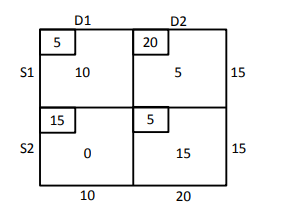
\includegraphics[width=0.75\columnwidth]{chapters/10/7/2/4/figs/fig.png}
 \end{center}
\caption{}
\label{fig:10/7/2/4Fig1}
\end{figure}
\fi

\item Find the position vector of the mid point of the vector joining the points $\vec{P}$(2, 3, 4)
and $\vec{Q}$(4, 1, –2).
\\
\solution
		\begin{enumerate}[label=\thesubsection.\arabic*,ref=\thesubsection.\theenumi]
\item Find the coordinates of the point which divides the join of $(-1,7) $ and $ (4,-3)$ in the ratio 2:3.
	\\
		\solution
	\input{chapters/10/7/2/1/section.tex}
\item Find the coordinates of the point $\vec{R}$ on the line segment joining the points $\vec{P}(-1,3)$ and $\vec{Q}(2,5)$ such that $PR=\frac{3}{5}PQ$.
\item Find the ratio in which the point $\vec{P}\brak{\frac{3}{4},\frac{5}{12}}$ divides the line segment joining the points $\vec{A}\brak{\frac{1}{2},\frac{3}{2}}$ and $ \vec{B}(2,-5)$.
\item Find the coordinates of the point which divides the line segment joining the points $(4,-3)$ and $(8,5)$ in the ratio $3:1$ internally.
\item Find the coordinates of the point $\vec{P}$ on $AD$ such that $AP : PD = 2 : 1$.
\item If the point $\vec{P} (2, 1)$ lies on the line segment joining points $\vec{A} (4, 2)$  and $ \vec{B} (8, 4)$,
then
\begin{enumerate}
	\item $AP =\frac{1}{3}{AB}$ 
\item ${AP}={PE}$
\item ${PB}=\frac{1}{3}{AB}$
\item${AP}=\frac{1}{2}{AB}$
 \end{enumerate}
\item Find the ratio in which the line segment joining the points $(-3,10)$  and  $(6,-8)$  is divided by $ (-1,6)$.
	\\
		\solution
	\input{chapters/10/7/2/4/section.tex}
\item Find the position vector of the mid point of the vector joining the points $\vec{P}$(2, 3, 4)
and $\vec{Q}$(4, 1, –2).
\\
\solution
		\input{chapters/12/10/2/16/section.tex}
\item Let $\vec{A}(4, 2), \vec{B}(6, 5)$  and $ \vec{C}(1, 4)$ be the vertices of $\triangle ABC$.
\begin{enumerate}
\item If $\vec{A}$ and  $\vec{B}$ are $(-2,-2)$ and  $(2,-4)$, respectively, find the coordinates of $\vec{P}$ such that $AP= \frac {3}{7}AB$  and $ \vec{P}$ lies on the line segment $AB$.
	\\
		\solution
	\input{chapters/10/7/2/8/section.tex}
\item Find the coordinates of the points which divide the line segment joining $A(-2,2)$  and  $\vec{B}(2,8)$ into four equal parts.
	\\
		\solution
	\input{chapters/10/7/2/9/section.tex}
\item In what ratio does the point $(-4,6)$ divide the line segment joining the points $\vec{A}(-6,0)$ and $\vec{B}(3,-8)$?
\item Given that $\vec{P}(3,2,-4), \vec{Q}(5,4,-6)$ and $\vec{R}(9,8,-10)$ are collinear. Find the ratio in which $\vec{Q}$ divides $PR$.
\item Points $\vec{A}(-6,10),\vec{B}(-4,6)$  and  $\vec{C}(3,-8)$ are collinear such that $AB=  \frac{2}{9}AC$.
\item The point which divides the line segment joining the points $\vec{P} (7, –6) $  and  $\vec{Q}(3, 4)$ in the 
ratio 1 : 2 internally lies in  which quadrant?
\item Find the coordinates of the points of trisection of the line segment joining $(4,-1)$  and  $(-2,3)$.
	\\
		\solution
	\input{chapters/10/7/2/2/section.tex}
\item Find the coordinates of the points which trisect the line segment joining the points $\vec{P}(4,2,-6)$ and $\vec{Q}(10,-16,6)$.
\item Find the coordinates of the points of trisection (i.e. points dividing to three equal parts) of the line segment joining the points $\vec{A}(2,-2)$ and $\vec{B}(-7,4)$.
\item Point $\vec{P}(5,-3)$ is one of the two points of trisection of line segment joining the points $\vec{A}(7,-2)$ and $\vec{B}(1,-5)$
\item Find the position vector of a point $\vec{R}$ which divides the line joining two points $\vec{P}$
and $\vec{Q}$ whose position vectors are $\hat{i}+2\hat{j}-\hat{k}$ and $-\hat{i}+\hat{j}+\hat{k}$ respectively, in the
ratio 2 : 1
\begin{enumerate}
    \item  internally
    \item  externally
\end{enumerate}
%\solution
%		\input{chapters/12/10/2/15/section.tex}
\item Find the coordinates of the point which divides the line segment joining the points which divides the line segment joining  the points $(-2,3,5)$ and $(1,-4,6)$ in the ratio 
\begin{enumerate}
\item $2:3$ internally,
\item $2:3$ externally
\end{enumerate}
\item Find the coordinates of the point which divides the line segment joining the points $(1,-2,3)$ and $(3,4,-5)$ in the ratio $2:3$
\begin{enumerate}
\item internally, and
\item externally
\end{enumerate}
\item Consider two points $\vec{P}$ and $\vec{Q}$ with position vectors $\overrightarrow{OP} = 3\overrightarrow{a}-2\overrightarrow{b}$ and $\overrightarrow{OQ}=\overrightarrow{a}+\overrightarrow{b}$. Find the position vector of a point $\vec{R}$ which divides the line joining $\vec{P}$ and $\vec{Q}$ in the ratio $2:1$, 
\begin{enumerate}
\item internally, and 
\item externally.
\end{enumerate}
\item The median from $\vec{A}$ meets $BC$ at $\vec{D}$. Find the coordinates of the point $\vec{D}$.
\item Find the coordinates of points $\vec{Q}$ and $\vec{R}$ on medians $BE$ and $CF$ respectively such that $BQ : QE = 2 : 1$  and  $CR : RF = 2 : 1$.
\item What do you observe?
\item If $\vec{A}, \vec{B}$ and $\vec{C}$  are the vertices of $\triangle ABC$, find the coordinates of the centroid of the triangle.
\end{enumerate}
\solution
	\input{chapters/10/7/4/7/section.tex}
\item If $\vec{P}(9a-2,-b)$ divides line segment joining $\vec{A}(3a+1,-3)$ and $\vec{B}(8a,5)$ in the ratio 3:1, find the values of $a$ and $b$.
\item Find the position vector of a point $\vec{R}$ which divides the line joining two points $\vec{P}$ and $\vec{Q}$ whose position vectors are $2\vec{a}+\vec{b}$ and $\vec{a}-3\vec{b}$ externally in the ratio $1:2$.
\item The position vector of the point which divides the join of points 2$\vec{a}$-3$\vec{b}$ $\text{and}$ $\vec{a}+\vec{b}$ in the ratio 3:1 is \rule{1cm}{0.1pt}.
\item If $\vec{a}$ and $\vec{b}$ are the postion vectors of $\vec{A}$ and $\vec{B}$, respectively, find the position vector of a point $\vec{C}$ in $BA$ produced such that $BC=1.5BA$.
\item Find the position vector of a point $\vec{R}$ which divides the line joining two points $\vec{P}$ and $\vec{Q}$ whose position vectors are $(2\vec{a}+\vec{b})$ and $(\vec{a}-3\vec{b})$
externally in the ratio 1 : 2. Also, show that $\vec{P}$ is the mid point of the line segment $RQ$.
\end{enumerate}

\item Let $\vec{A}(4, 2), \vec{B}(6, 5)$  and $ \vec{C}(1, 4)$ be the vertices of $\triangle ABC$.
\begin{enumerate}
\item If $\vec{A}$ and  $\vec{B}$ are $(-2,-2)$ and  $(2,-4)$, respectively, find the coordinates of $\vec{P}$ such that $AP= \frac {3}{7}AB$  and $ \vec{P}$ lies on the line segment $AB$.
	\\
		\solution
	\begin{enumerate}[label=\thesubsection.\arabic*,ref=\thesubsection.\theenumi]
\item Find the coordinates of the point which divides the join of $(-1,7) $ and $ (4,-3)$ in the ratio 2:3.
	\\
		\solution
	\input{chapters/10/7/2/1/section.tex}
\item Find the coordinates of the point $\vec{R}$ on the line segment joining the points $\vec{P}(-1,3)$ and $\vec{Q}(2,5)$ such that $PR=\frac{3}{5}PQ$.
\item Find the ratio in which the point $\vec{P}\brak{\frac{3}{4},\frac{5}{12}}$ divides the line segment joining the points $\vec{A}\brak{\frac{1}{2},\frac{3}{2}}$ and $ \vec{B}(2,-5)$.
\item Find the coordinates of the point which divides the line segment joining the points $(4,-3)$ and $(8,5)$ in the ratio $3:1$ internally.
\item Find the coordinates of the point $\vec{P}$ on $AD$ such that $AP : PD = 2 : 1$.
\item If the point $\vec{P} (2, 1)$ lies on the line segment joining points $\vec{A} (4, 2)$  and $ \vec{B} (8, 4)$,
then
\begin{enumerate}
	\item $AP =\frac{1}{3}{AB}$ 
\item ${AP}={PE}$
\item ${PB}=\frac{1}{3}{AB}$
\item${AP}=\frac{1}{2}{AB}$
 \end{enumerate}
\item Find the ratio in which the line segment joining the points $(-3,10)$  and  $(6,-8)$  is divided by $ (-1,6)$.
	\\
		\solution
	\input{chapters/10/7/2/4/section.tex}
\item Find the position vector of the mid point of the vector joining the points $\vec{P}$(2, 3, 4)
and $\vec{Q}$(4, 1, –2).
\\
\solution
		\input{chapters/12/10/2/16/section.tex}
\item Let $\vec{A}(4, 2), \vec{B}(6, 5)$  and $ \vec{C}(1, 4)$ be the vertices of $\triangle ABC$.
\begin{enumerate}
\item If $\vec{A}$ and  $\vec{B}$ are $(-2,-2)$ and  $(2,-4)$, respectively, find the coordinates of $\vec{P}$ such that $AP= \frac {3}{7}AB$  and $ \vec{P}$ lies on the line segment $AB$.
	\\
		\solution
	\input{chapters/10/7/2/8/section.tex}
\item Find the coordinates of the points which divide the line segment joining $A(-2,2)$  and  $\vec{B}(2,8)$ into four equal parts.
	\\
		\solution
	\input{chapters/10/7/2/9/section.tex}
\item In what ratio does the point $(-4,6)$ divide the line segment joining the points $\vec{A}(-6,0)$ and $\vec{B}(3,-8)$?
\item Given that $\vec{P}(3,2,-4), \vec{Q}(5,4,-6)$ and $\vec{R}(9,8,-10)$ are collinear. Find the ratio in which $\vec{Q}$ divides $PR$.
\item Points $\vec{A}(-6,10),\vec{B}(-4,6)$  and  $\vec{C}(3,-8)$ are collinear such that $AB=  \frac{2}{9}AC$.
\item The point which divides the line segment joining the points $\vec{P} (7, –6) $  and  $\vec{Q}(3, 4)$ in the 
ratio 1 : 2 internally lies in  which quadrant?
\item Find the coordinates of the points of trisection of the line segment joining $(4,-1)$  and  $(-2,3)$.
	\\
		\solution
	\input{chapters/10/7/2/2/section.tex}
\item Find the coordinates of the points which trisect the line segment joining the points $\vec{P}(4,2,-6)$ and $\vec{Q}(10,-16,6)$.
\item Find the coordinates of the points of trisection (i.e. points dividing to three equal parts) of the line segment joining the points $\vec{A}(2,-2)$ and $\vec{B}(-7,4)$.
\item Point $\vec{P}(5,-3)$ is one of the two points of trisection of line segment joining the points $\vec{A}(7,-2)$ and $\vec{B}(1,-5)$
\item Find the position vector of a point $\vec{R}$ which divides the line joining two points $\vec{P}$
and $\vec{Q}$ whose position vectors are $\hat{i}+2\hat{j}-\hat{k}$ and $-\hat{i}+\hat{j}+\hat{k}$ respectively, in the
ratio 2 : 1
\begin{enumerate}
    \item  internally
    \item  externally
\end{enumerate}
%\solution
%		\input{chapters/12/10/2/15/section.tex}
\item Find the coordinates of the point which divides the line segment joining the points which divides the line segment joining  the points $(-2,3,5)$ and $(1,-4,6)$ in the ratio 
\begin{enumerate}
\item $2:3$ internally,
\item $2:3$ externally
\end{enumerate}
\item Find the coordinates of the point which divides the line segment joining the points $(1,-2,3)$ and $(3,4,-5)$ in the ratio $2:3$
\begin{enumerate}
\item internally, and
\item externally
\end{enumerate}
\item Consider two points $\vec{P}$ and $\vec{Q}$ with position vectors $\overrightarrow{OP} = 3\overrightarrow{a}-2\overrightarrow{b}$ and $\overrightarrow{OQ}=\overrightarrow{a}+\overrightarrow{b}$. Find the position vector of a point $\vec{R}$ which divides the line joining $\vec{P}$ and $\vec{Q}$ in the ratio $2:1$, 
\begin{enumerate}
\item internally, and 
\item externally.
\end{enumerate}
\item The median from $\vec{A}$ meets $BC$ at $\vec{D}$. Find the coordinates of the point $\vec{D}$.
\item Find the coordinates of points $\vec{Q}$ and $\vec{R}$ on medians $BE$ and $CF$ respectively such that $BQ : QE = 2 : 1$  and  $CR : RF = 2 : 1$.
\item What do you observe?
\item If $\vec{A}, \vec{B}$ and $\vec{C}$  are the vertices of $\triangle ABC$, find the coordinates of the centroid of the triangle.
\end{enumerate}
\solution
	\input{chapters/10/7/4/7/section.tex}
\item If $\vec{P}(9a-2,-b)$ divides line segment joining $\vec{A}(3a+1,-3)$ and $\vec{B}(8a,5)$ in the ratio 3:1, find the values of $a$ and $b$.
\item Find the position vector of a point $\vec{R}$ which divides the line joining two points $\vec{P}$ and $\vec{Q}$ whose position vectors are $2\vec{a}+\vec{b}$ and $\vec{a}-3\vec{b}$ externally in the ratio $1:2$.
\item The position vector of the point which divides the join of points 2$\vec{a}$-3$\vec{b}$ $\text{and}$ $\vec{a}+\vec{b}$ in the ratio 3:1 is \rule{1cm}{0.1pt}.
\item If $\vec{a}$ and $\vec{b}$ are the postion vectors of $\vec{A}$ and $\vec{B}$, respectively, find the position vector of a point $\vec{C}$ in $BA$ produced such that $BC=1.5BA$.
\item Find the position vector of a point $\vec{R}$ which divides the line joining two points $\vec{P}$ and $\vec{Q}$ whose position vectors are $(2\vec{a}+\vec{b})$ and $(\vec{a}-3\vec{b})$
externally in the ratio 1 : 2. Also, show that $\vec{P}$ is the mid point of the line segment $RQ$.
\end{enumerate}

\item Find the coordinates of the points which divide the line segment joining $A(-2,2)$  and  $\vec{B}(2,8)$ into four equal parts.
	\\
		\solution
	\begin{enumerate}[label=\thesubsection.\arabic*,ref=\thesubsection.\theenumi]
\item Find the coordinates of the point which divides the join of $(-1,7) $ and $ (4,-3)$ in the ratio 2:3.
	\\
		\solution
	\input{chapters/10/7/2/1/section.tex}
\item Find the coordinates of the point $\vec{R}$ on the line segment joining the points $\vec{P}(-1,3)$ and $\vec{Q}(2,5)$ such that $PR=\frac{3}{5}PQ$.
\item Find the ratio in which the point $\vec{P}\brak{\frac{3}{4},\frac{5}{12}}$ divides the line segment joining the points $\vec{A}\brak{\frac{1}{2},\frac{3}{2}}$ and $ \vec{B}(2,-5)$.
\item Find the coordinates of the point which divides the line segment joining the points $(4,-3)$ and $(8,5)$ in the ratio $3:1$ internally.
\item Find the coordinates of the point $\vec{P}$ on $AD$ such that $AP : PD = 2 : 1$.
\item If the point $\vec{P} (2, 1)$ lies on the line segment joining points $\vec{A} (4, 2)$  and $ \vec{B} (8, 4)$,
then
\begin{enumerate}
	\item $AP =\frac{1}{3}{AB}$ 
\item ${AP}={PE}$
\item ${PB}=\frac{1}{3}{AB}$
\item${AP}=\frac{1}{2}{AB}$
 \end{enumerate}
\item Find the ratio in which the line segment joining the points $(-3,10)$  and  $(6,-8)$  is divided by $ (-1,6)$.
	\\
		\solution
	\input{chapters/10/7/2/4/section.tex}
\item Find the position vector of the mid point of the vector joining the points $\vec{P}$(2, 3, 4)
and $\vec{Q}$(4, 1, –2).
\\
\solution
		\input{chapters/12/10/2/16/section.tex}
\item Let $\vec{A}(4, 2), \vec{B}(6, 5)$  and $ \vec{C}(1, 4)$ be the vertices of $\triangle ABC$.
\begin{enumerate}
\item If $\vec{A}$ and  $\vec{B}$ are $(-2,-2)$ and  $(2,-4)$, respectively, find the coordinates of $\vec{P}$ such that $AP= \frac {3}{7}AB$  and $ \vec{P}$ lies on the line segment $AB$.
	\\
		\solution
	\input{chapters/10/7/2/8/section.tex}
\item Find the coordinates of the points which divide the line segment joining $A(-2,2)$  and  $\vec{B}(2,8)$ into four equal parts.
	\\
		\solution
	\input{chapters/10/7/2/9/section.tex}
\item In what ratio does the point $(-4,6)$ divide the line segment joining the points $\vec{A}(-6,0)$ and $\vec{B}(3,-8)$?
\item Given that $\vec{P}(3,2,-4), \vec{Q}(5,4,-6)$ and $\vec{R}(9,8,-10)$ are collinear. Find the ratio in which $\vec{Q}$ divides $PR$.
\item Points $\vec{A}(-6,10),\vec{B}(-4,6)$  and  $\vec{C}(3,-8)$ are collinear such that $AB=  \frac{2}{9}AC$.
\item The point which divides the line segment joining the points $\vec{P} (7, –6) $  and  $\vec{Q}(3, 4)$ in the 
ratio 1 : 2 internally lies in  which quadrant?
\item Find the coordinates of the points of trisection of the line segment joining $(4,-1)$  and  $(-2,3)$.
	\\
		\solution
	\input{chapters/10/7/2/2/section.tex}
\item Find the coordinates of the points which trisect the line segment joining the points $\vec{P}(4,2,-6)$ and $\vec{Q}(10,-16,6)$.
\item Find the coordinates of the points of trisection (i.e. points dividing to three equal parts) of the line segment joining the points $\vec{A}(2,-2)$ and $\vec{B}(-7,4)$.
\item Point $\vec{P}(5,-3)$ is one of the two points of trisection of line segment joining the points $\vec{A}(7,-2)$ and $\vec{B}(1,-5)$
\item Find the position vector of a point $\vec{R}$ which divides the line joining two points $\vec{P}$
and $\vec{Q}$ whose position vectors are $\hat{i}+2\hat{j}-\hat{k}$ and $-\hat{i}+\hat{j}+\hat{k}$ respectively, in the
ratio 2 : 1
\begin{enumerate}
    \item  internally
    \item  externally
\end{enumerate}
%\solution
%		\input{chapters/12/10/2/15/section.tex}
\item Find the coordinates of the point which divides the line segment joining the points which divides the line segment joining  the points $(-2,3,5)$ and $(1,-4,6)$ in the ratio 
\begin{enumerate}
\item $2:3$ internally,
\item $2:3$ externally
\end{enumerate}
\item Find the coordinates of the point which divides the line segment joining the points $(1,-2,3)$ and $(3,4,-5)$ in the ratio $2:3$
\begin{enumerate}
\item internally, and
\item externally
\end{enumerate}
\item Consider two points $\vec{P}$ and $\vec{Q}$ with position vectors $\overrightarrow{OP} = 3\overrightarrow{a}-2\overrightarrow{b}$ and $\overrightarrow{OQ}=\overrightarrow{a}+\overrightarrow{b}$. Find the position vector of a point $\vec{R}$ which divides the line joining $\vec{P}$ and $\vec{Q}$ in the ratio $2:1$, 
\begin{enumerate}
\item internally, and 
\item externally.
\end{enumerate}
\item The median from $\vec{A}$ meets $BC$ at $\vec{D}$. Find the coordinates of the point $\vec{D}$.
\item Find the coordinates of points $\vec{Q}$ and $\vec{R}$ on medians $BE$ and $CF$ respectively such that $BQ : QE = 2 : 1$  and  $CR : RF = 2 : 1$.
\item What do you observe?
\item If $\vec{A}, \vec{B}$ and $\vec{C}$  are the vertices of $\triangle ABC$, find the coordinates of the centroid of the triangle.
\end{enumerate}
\solution
	\input{chapters/10/7/4/7/section.tex}
\item If $\vec{P}(9a-2,-b)$ divides line segment joining $\vec{A}(3a+1,-3)$ and $\vec{B}(8a,5)$ in the ratio 3:1, find the values of $a$ and $b$.
\item Find the position vector of a point $\vec{R}$ which divides the line joining two points $\vec{P}$ and $\vec{Q}$ whose position vectors are $2\vec{a}+\vec{b}$ and $\vec{a}-3\vec{b}$ externally in the ratio $1:2$.
\item The position vector of the point which divides the join of points 2$\vec{a}$-3$\vec{b}$ $\text{and}$ $\vec{a}+\vec{b}$ in the ratio 3:1 is \rule{1cm}{0.1pt}.
\item If $\vec{a}$ and $\vec{b}$ are the postion vectors of $\vec{A}$ and $\vec{B}$, respectively, find the position vector of a point $\vec{C}$ in $BA$ produced such that $BC=1.5BA$.
\item Find the position vector of a point $\vec{R}$ which divides the line joining two points $\vec{P}$ and $\vec{Q}$ whose position vectors are $(2\vec{a}+\vec{b})$ and $(\vec{a}-3\vec{b})$
externally in the ratio 1 : 2. Also, show that $\vec{P}$ is the mid point of the line segment $RQ$.
\end{enumerate}

\item In what ratio does the point $(-4,6)$ divide the line segment joining the points $\vec{A}(-6,0)$ and $\vec{B}(3,-8)$?
\item Given that $\vec{P}(3,2,-4), \vec{Q}(5,4,-6)$ and $\vec{R}(9,8,-10)$ are collinear. Find the ratio in which $\vec{Q}$ divides $PR$.
\item Points $\vec{A}(-6,10),\vec{B}(-4,6)$  and  $\vec{C}(3,-8)$ are collinear such that $AB=  \frac{2}{9}AC$.
\item The point which divides the line segment joining the points $\vec{P} (7, –6) $  and  $\vec{Q}(3, 4)$ in the 
ratio 1 : 2 internally lies in  which quadrant?
\item Find the coordinates of the points of trisection of the line segment joining $(4,-1)$  and  $(-2,3)$.
	\\
		\solution
	Using section formula,
\begin{align}
\vec{R}=\frac{1}{1+\frac{1}{2}}\brak{\myvec{4\\-1}+\frac{1}{2}\myvec{-2\\3}}
=\myvec{2\\ \frac{1}{3}}\\
\vec{S}=\frac{1}{1+\frac{2}{1}}\brak{\myvec{4\\-1}+\frac{2}{1}\myvec{-2\\3}}
=\myvec{0\\ \frac{5}{3}}
\end{align}
which are the desired points of trisection.
\iffalse
See
		\figref{fig:chapters/10/7/2/2/Figure}
\begin{figure}[H]
\centering
\includegraphics[width=0.75\columnwidth]{chapters/10/7/2/2/figs/dj.pdf}
\caption{}
		\label{fig:chapters/10/7/2/2/Figure}
\end{figure}
\fi

\item Find the coordinates of the points which trisect the line segment joining the points $\vec{P}(4,2,-6)$ and $\vec{Q}(10,-16,6)$.
\item Find the coordinates of the points of trisection (i.e. points dividing to three equal parts) of the line segment joining the points $\vec{A}(2,-2)$ and $\vec{B}(-7,4)$.
\item Point $\vec{P}(5,-3)$ is one of the two points of trisection of line segment joining the points $\vec{A}(7,-2)$ and $\vec{B}(1,-5)$
\item Find the position vector of a point $\vec{R}$ which divides the line joining two points $\vec{P}$
and $\vec{Q}$ whose position vectors are $\hat{i}+2\hat{j}-\hat{k}$ and $-\hat{i}+\hat{j}+\hat{k}$ respectively, in the
ratio 2 : 1
\begin{enumerate}
    \item  internally
    \item  externally
\end{enumerate}
%\solution
%		\begin{enumerate}[label=\thesubsection.\arabic*,ref=\thesubsection.\theenumi]
\item Find the coordinates of the point which divides the join of $(-1,7) $ and $ (4,-3)$ in the ratio 2:3.
	\\
		\solution
	\input{chapters/10/7/2/1/section.tex}
\item Find the coordinates of the point $\vec{R}$ on the line segment joining the points $\vec{P}(-1,3)$ and $\vec{Q}(2,5)$ such that $PR=\frac{3}{5}PQ$.
\item Find the ratio in which the point $\vec{P}\brak{\frac{3}{4},\frac{5}{12}}$ divides the line segment joining the points $\vec{A}\brak{\frac{1}{2},\frac{3}{2}}$ and $ \vec{B}(2,-5)$.
\item Find the coordinates of the point which divides the line segment joining the points $(4,-3)$ and $(8,5)$ in the ratio $3:1$ internally.
\item Find the coordinates of the point $\vec{P}$ on $AD$ such that $AP : PD = 2 : 1$.
\item If the point $\vec{P} (2, 1)$ lies on the line segment joining points $\vec{A} (4, 2)$  and $ \vec{B} (8, 4)$,
then
\begin{enumerate}
	\item $AP =\frac{1}{3}{AB}$ 
\item ${AP}={PE}$
\item ${PB}=\frac{1}{3}{AB}$
\item${AP}=\frac{1}{2}{AB}$
 \end{enumerate}
\item Find the ratio in which the line segment joining the points $(-3,10)$  and  $(6,-8)$  is divided by $ (-1,6)$.
	\\
		\solution
	\input{chapters/10/7/2/4/section.tex}
\item Find the position vector of the mid point of the vector joining the points $\vec{P}$(2, 3, 4)
and $\vec{Q}$(4, 1, –2).
\\
\solution
		\input{chapters/12/10/2/16/section.tex}
\item Let $\vec{A}(4, 2), \vec{B}(6, 5)$  and $ \vec{C}(1, 4)$ be the vertices of $\triangle ABC$.
\begin{enumerate}
\item If $\vec{A}$ and  $\vec{B}$ are $(-2,-2)$ and  $(2,-4)$, respectively, find the coordinates of $\vec{P}$ such that $AP= \frac {3}{7}AB$  and $ \vec{P}$ lies on the line segment $AB$.
	\\
		\solution
	\input{chapters/10/7/2/8/section.tex}
\item Find the coordinates of the points which divide the line segment joining $A(-2,2)$  and  $\vec{B}(2,8)$ into four equal parts.
	\\
		\solution
	\input{chapters/10/7/2/9/section.tex}
\item In what ratio does the point $(-4,6)$ divide the line segment joining the points $\vec{A}(-6,0)$ and $\vec{B}(3,-8)$?
\item Given that $\vec{P}(3,2,-4), \vec{Q}(5,4,-6)$ and $\vec{R}(9,8,-10)$ are collinear. Find the ratio in which $\vec{Q}$ divides $PR$.
\item Points $\vec{A}(-6,10),\vec{B}(-4,6)$  and  $\vec{C}(3,-8)$ are collinear such that $AB=  \frac{2}{9}AC$.
\item The point which divides the line segment joining the points $\vec{P} (7, –6) $  and  $\vec{Q}(3, 4)$ in the 
ratio 1 : 2 internally lies in  which quadrant?
\item Find the coordinates of the points of trisection of the line segment joining $(4,-1)$  and  $(-2,3)$.
	\\
		\solution
	\input{chapters/10/7/2/2/section.tex}
\item Find the coordinates of the points which trisect the line segment joining the points $\vec{P}(4,2,-6)$ and $\vec{Q}(10,-16,6)$.
\item Find the coordinates of the points of trisection (i.e. points dividing to three equal parts) of the line segment joining the points $\vec{A}(2,-2)$ and $\vec{B}(-7,4)$.
\item Point $\vec{P}(5,-3)$ is one of the two points of trisection of line segment joining the points $\vec{A}(7,-2)$ and $\vec{B}(1,-5)$
\item Find the position vector of a point $\vec{R}$ which divides the line joining two points $\vec{P}$
and $\vec{Q}$ whose position vectors are $\hat{i}+2\hat{j}-\hat{k}$ and $-\hat{i}+\hat{j}+\hat{k}$ respectively, in the
ratio 2 : 1
\begin{enumerate}
    \item  internally
    \item  externally
\end{enumerate}
%\solution
%		\input{chapters/12/10/2/15/section.tex}
\item Find the coordinates of the point which divides the line segment joining the points which divides the line segment joining  the points $(-2,3,5)$ and $(1,-4,6)$ in the ratio 
\begin{enumerate}
\item $2:3$ internally,
\item $2:3$ externally
\end{enumerate}
\item Find the coordinates of the point which divides the line segment joining the points $(1,-2,3)$ and $(3,4,-5)$ in the ratio $2:3$
\begin{enumerate}
\item internally, and
\item externally
\end{enumerate}
\item Consider two points $\vec{P}$ and $\vec{Q}$ with position vectors $\overrightarrow{OP} = 3\overrightarrow{a}-2\overrightarrow{b}$ and $\overrightarrow{OQ}=\overrightarrow{a}+\overrightarrow{b}$. Find the position vector of a point $\vec{R}$ which divides the line joining $\vec{P}$ and $\vec{Q}$ in the ratio $2:1$, 
\begin{enumerate}
\item internally, and 
\item externally.
\end{enumerate}
\item The median from $\vec{A}$ meets $BC$ at $\vec{D}$. Find the coordinates of the point $\vec{D}$.
\item Find the coordinates of points $\vec{Q}$ and $\vec{R}$ on medians $BE$ and $CF$ respectively such that $BQ : QE = 2 : 1$  and  $CR : RF = 2 : 1$.
\item What do you observe?
\item If $\vec{A}, \vec{B}$ and $\vec{C}$  are the vertices of $\triangle ABC$, find the coordinates of the centroid of the triangle.
\end{enumerate}
\solution
	\input{chapters/10/7/4/7/section.tex}
\item If $\vec{P}(9a-2,-b)$ divides line segment joining $\vec{A}(3a+1,-3)$ and $\vec{B}(8a,5)$ in the ratio 3:1, find the values of $a$ and $b$.
\item Find the position vector of a point $\vec{R}$ which divides the line joining two points $\vec{P}$ and $\vec{Q}$ whose position vectors are $2\vec{a}+\vec{b}$ and $\vec{a}-3\vec{b}$ externally in the ratio $1:2$.
\item The position vector of the point which divides the join of points 2$\vec{a}$-3$\vec{b}$ $\text{and}$ $\vec{a}+\vec{b}$ in the ratio 3:1 is \rule{1cm}{0.1pt}.
\item If $\vec{a}$ and $\vec{b}$ are the postion vectors of $\vec{A}$ and $\vec{B}$, respectively, find the position vector of a point $\vec{C}$ in $BA$ produced such that $BC=1.5BA$.
\item Find the position vector of a point $\vec{R}$ which divides the line joining two points $\vec{P}$ and $\vec{Q}$ whose position vectors are $(2\vec{a}+\vec{b})$ and $(\vec{a}-3\vec{b})$
externally in the ratio 1 : 2. Also, show that $\vec{P}$ is the mid point of the line segment $RQ$.
\end{enumerate}

\item Find the coordinates of the point which divides the line segment joining the points which divides the line segment joining  the points $(-2,3,5)$ and $(1,-4,6)$ in the ratio 
\begin{enumerate}
\item $2:3$ internally,
\item $2:3$ externally
\end{enumerate}
\item Find the coordinates of the point which divides the line segment joining the points $(1,-2,3)$ and $(3,4,-5)$ in the ratio $2:3$
\begin{enumerate}
\item internally, and
\item externally
\end{enumerate}
\item Consider two points $\vec{P}$ and $\vec{Q}$ with position vectors $\overrightarrow{OP} = 3\overrightarrow{a}-2\overrightarrow{b}$ and $\overrightarrow{OQ}=\overrightarrow{a}+\overrightarrow{b}$. Find the position vector of a point $\vec{R}$ which divides the line joining $\vec{P}$ and $\vec{Q}$ in the ratio $2:1$, 
\begin{enumerate}
\item internally, and 
\item externally.
\end{enumerate}
\item The median from $\vec{A}$ meets $BC$ at $\vec{D}$. Find the coordinates of the point $\vec{D}$.
\item Find the coordinates of points $\vec{Q}$ and $\vec{R}$ on medians $BE$ and $CF$ respectively such that $BQ : QE = 2 : 1$  and  $CR : RF = 2 : 1$.
\item What do you observe?
\item If $\vec{A}, \vec{B}$ and $\vec{C}$  are the vertices of $\triangle ABC$, find the coordinates of the centroid of the triangle.
\end{enumerate}
\solution
	\begin{enumerate}[label=\thesubsection.\arabic*,ref=\thesubsection.\theenumi]
\item Find the coordinates of the point which divides the join of $(-1,7) $ and $ (4,-3)$ in the ratio 2:3.
	\\
		\solution
	\input{chapters/10/7/2/1/section.tex}
\item Find the coordinates of the point $\vec{R}$ on the line segment joining the points $\vec{P}(-1,3)$ and $\vec{Q}(2,5)$ such that $PR=\frac{3}{5}PQ$.
\item Find the ratio in which the point $\vec{P}\brak{\frac{3}{4},\frac{5}{12}}$ divides the line segment joining the points $\vec{A}\brak{\frac{1}{2},\frac{3}{2}}$ and $ \vec{B}(2,-5)$.
\item Find the coordinates of the point which divides the line segment joining the points $(4,-3)$ and $(8,5)$ in the ratio $3:1$ internally.
\item Find the coordinates of the point $\vec{P}$ on $AD$ such that $AP : PD = 2 : 1$.
\item If the point $\vec{P} (2, 1)$ lies on the line segment joining points $\vec{A} (4, 2)$  and $ \vec{B} (8, 4)$,
then
\begin{enumerate}
	\item $AP =\frac{1}{3}{AB}$ 
\item ${AP}={PE}$
\item ${PB}=\frac{1}{3}{AB}$
\item${AP}=\frac{1}{2}{AB}$
 \end{enumerate}
\item Find the ratio in which the line segment joining the points $(-3,10)$  and  $(6,-8)$  is divided by $ (-1,6)$.
	\\
		\solution
	\input{chapters/10/7/2/4/section.tex}
\item Find the position vector of the mid point of the vector joining the points $\vec{P}$(2, 3, 4)
and $\vec{Q}$(4, 1, –2).
\\
\solution
		\input{chapters/12/10/2/16/section.tex}
\item Let $\vec{A}(4, 2), \vec{B}(6, 5)$  and $ \vec{C}(1, 4)$ be the vertices of $\triangle ABC$.
\begin{enumerate}
\item If $\vec{A}$ and  $\vec{B}$ are $(-2,-2)$ and  $(2,-4)$, respectively, find the coordinates of $\vec{P}$ such that $AP= \frac {3}{7}AB$  and $ \vec{P}$ lies on the line segment $AB$.
	\\
		\solution
	\input{chapters/10/7/2/8/section.tex}
\item Find the coordinates of the points which divide the line segment joining $A(-2,2)$  and  $\vec{B}(2,8)$ into four equal parts.
	\\
		\solution
	\input{chapters/10/7/2/9/section.tex}
\item In what ratio does the point $(-4,6)$ divide the line segment joining the points $\vec{A}(-6,0)$ and $\vec{B}(3,-8)$?
\item Given that $\vec{P}(3,2,-4), \vec{Q}(5,4,-6)$ and $\vec{R}(9,8,-10)$ are collinear. Find the ratio in which $\vec{Q}$ divides $PR$.
\item Points $\vec{A}(-6,10),\vec{B}(-4,6)$  and  $\vec{C}(3,-8)$ are collinear such that $AB=  \frac{2}{9}AC$.
\item The point which divides the line segment joining the points $\vec{P} (7, –6) $  and  $\vec{Q}(3, 4)$ in the 
ratio 1 : 2 internally lies in  which quadrant?
\item Find the coordinates of the points of trisection of the line segment joining $(4,-1)$  and  $(-2,3)$.
	\\
		\solution
	\input{chapters/10/7/2/2/section.tex}
\item Find the coordinates of the points which trisect the line segment joining the points $\vec{P}(4,2,-6)$ and $\vec{Q}(10,-16,6)$.
\item Find the coordinates of the points of trisection (i.e. points dividing to three equal parts) of the line segment joining the points $\vec{A}(2,-2)$ and $\vec{B}(-7,4)$.
\item Point $\vec{P}(5,-3)$ is one of the two points of trisection of line segment joining the points $\vec{A}(7,-2)$ and $\vec{B}(1,-5)$
\item Find the position vector of a point $\vec{R}$ which divides the line joining two points $\vec{P}$
and $\vec{Q}$ whose position vectors are $\hat{i}+2\hat{j}-\hat{k}$ and $-\hat{i}+\hat{j}+\hat{k}$ respectively, in the
ratio 2 : 1
\begin{enumerate}
    \item  internally
    \item  externally
\end{enumerate}
%\solution
%		\input{chapters/12/10/2/15/section.tex}
\item Find the coordinates of the point which divides the line segment joining the points which divides the line segment joining  the points $(-2,3,5)$ and $(1,-4,6)$ in the ratio 
\begin{enumerate}
\item $2:3$ internally,
\item $2:3$ externally
\end{enumerate}
\item Find the coordinates of the point which divides the line segment joining the points $(1,-2,3)$ and $(3,4,-5)$ in the ratio $2:3$
\begin{enumerate}
\item internally, and
\item externally
\end{enumerate}
\item Consider two points $\vec{P}$ and $\vec{Q}$ with position vectors $\overrightarrow{OP} = 3\overrightarrow{a}-2\overrightarrow{b}$ and $\overrightarrow{OQ}=\overrightarrow{a}+\overrightarrow{b}$. Find the position vector of a point $\vec{R}$ which divides the line joining $\vec{P}$ and $\vec{Q}$ in the ratio $2:1$, 
\begin{enumerate}
\item internally, and 
\item externally.
\end{enumerate}
\item The median from $\vec{A}$ meets $BC$ at $\vec{D}$. Find the coordinates of the point $\vec{D}$.
\item Find the coordinates of points $\vec{Q}$ and $\vec{R}$ on medians $BE$ and $CF$ respectively such that $BQ : QE = 2 : 1$  and  $CR : RF = 2 : 1$.
\item What do you observe?
\item If $\vec{A}, \vec{B}$ and $\vec{C}$  are the vertices of $\triangle ABC$, find the coordinates of the centroid of the triangle.
\end{enumerate}
\solution
	\input{chapters/10/7/4/7/section.tex}
\item If $\vec{P}(9a-2,-b)$ divides line segment joining $\vec{A}(3a+1,-3)$ and $\vec{B}(8a,5)$ in the ratio 3:1, find the values of $a$ and $b$.
\item Find the position vector of a point $\vec{R}$ which divides the line joining two points $\vec{P}$ and $\vec{Q}$ whose position vectors are $2\vec{a}+\vec{b}$ and $\vec{a}-3\vec{b}$ externally in the ratio $1:2$.
\item The position vector of the point which divides the join of points 2$\vec{a}$-3$\vec{b}$ $\text{and}$ $\vec{a}+\vec{b}$ in the ratio 3:1 is \rule{1cm}{0.1pt}.
\item If $\vec{a}$ and $\vec{b}$ are the postion vectors of $\vec{A}$ and $\vec{B}$, respectively, find the position vector of a point $\vec{C}$ in $BA$ produced such that $BC=1.5BA$.
\item Find the position vector of a point $\vec{R}$ which divides the line joining two points $\vec{P}$ and $\vec{Q}$ whose position vectors are $(2\vec{a}+\vec{b})$ and $(\vec{a}-3\vec{b})$
externally in the ratio 1 : 2. Also, show that $\vec{P}$ is the mid point of the line segment $RQ$.
\end{enumerate}

\item If $\vec{P}(9a-2,-b)$ divides line segment joining $\vec{A}(3a+1,-3)$ and $\vec{B}(8a,5)$ in the ratio 3:1, find the values of $a$ and $b$.
\item Find the position vector of a point $\vec{R}$ which divides the line joining two points $\vec{P}$ and $\vec{Q}$ whose position vectors are $2\vec{a}+\vec{b}$ and $\vec{a}-3\vec{b}$ externally in the ratio $1:2$.
\item The position vector of the point which divides the join of points 2$\vec{a}$-3$\vec{b}$ $\text{and}$ $\vec{a}+\vec{b}$ in the ratio 3:1 is \rule{1cm}{0.1pt}.
\item If $\vec{a}$ and $\vec{b}$ are the postion vectors of $\vec{A}$ and $\vec{B}$, respectively, find the position vector of a point $\vec{C}$ in $BA$ produced such that $BC=1.5BA$.
\item Find the position vector of a point $\vec{R}$ which divides the line joining two points $\vec{P}$ and $\vec{Q}$ whose position vectors are $(2\vec{a}+\vec{b})$ and $(\vec{a}-3\vec{b})$
externally in the ratio 1 : 2. Also, show that $\vec{P}$ is the mid point of the line segment $RQ$.
\end{enumerate}

\item Find the coordinates of the point $\vec{R}$ on the line segment joining the points $\vec{P}(-1,3)$ and $\vec{Q}(2,5)$ such that $PR=\frac{3}{5}PQ$.
\item Find the ratio in which the point $\vec{P}\brak{\frac{3}{4},\frac{5}{12}}$ divides the line segment joining the points $\vec{A}\brak{\frac{1}{2},\frac{3}{2}}$ and $ \vec{B}(2,-5)$.
\item Find the coordinates of the point which divides the line segment joining the points $(4,-3)$ and $(8,5)$ in the ratio $3:1$ internally.
\item Find the coordinates of the point $\vec{P}$ on $AD$ such that $AP : PD = 2 : 1$.
\item If the point $\vec{P} (2, 1)$ lies on the line segment joining points $\vec{A} (4, 2)$  and $ \vec{B} (8, 4)$,
then
\begin{enumerate}
	\item $AP =\frac{1}{3}{AB}$ 
\item ${AP}={PE}$
\item ${PB}=\frac{1}{3}{AB}$
\item${AP}=\frac{1}{2}{AB}$
 \end{enumerate}
\item Find the ratio in which the line segment joining the points $(-3,10)$  and  $(6,-8)$  is divided by $ (-1,6)$.
	\\
		\solution
	\iffalse
Using section formula,
\begin{align}
         \myvec{-1\\6} &=\frac{{\myvec{-3\\10}+k\myvec{6\\-8}}}{1+k}\\
	 \implies 7k\myvec{1 \\ -2} &= 2\myvec{1 \\ -2}
	 \\
	 \text{or, } k &= \frac{2}{7}.
\end{align}
\fi
In 
			\eqref{eq:section_formula-k}, substituting
			\begin{align}
				\vec{B} &= \myvec{-3\\10}, \vec{C} = \myvec{6\\-8}, \vec{D} = \myvec{-1\\6},
				\\
				k &= \frac{\myvec{-2 & 4}\myvec{-7 \\ 14}}{\norm{\myvec{-7 \\ 14}}^2} = \frac{2}{7}
			\end{align}
\iffalse
See \figref{fig:10/7/2/4Fig1}.
\begin{figure}[H]
 \begin{center}
  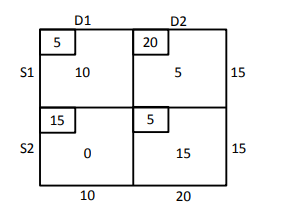
\includegraphics[width=0.75\columnwidth]{chapters/10/7/2/4/figs/fig.png}
 \end{center}
\caption{}
\label{fig:10/7/2/4Fig1}
\end{figure}
\fi

\item Find the position vector of the mid point of the vector joining the points $\vec{P}$(2, 3, 4)
and $\vec{Q}$(4, 1, –2).
\\
\solution
		\begin{enumerate}[label=\thesubsection.\arabic*,ref=\thesubsection.\theenumi]
\item Find the coordinates of the point which divides the join of $(-1,7) $ and $ (4,-3)$ in the ratio 2:3.
	\\
		\solution
	\begin{enumerate}[label=\thesubsection.\arabic*,ref=\thesubsection.\theenumi]
\item Find the coordinates of the point which divides the join of $(-1,7) $ and $ (4,-3)$ in the ratio 2:3.
	\\
		\solution
	\input{chapters/10/7/2/1/section.tex}
\item Find the coordinates of the point $\vec{R}$ on the line segment joining the points $\vec{P}(-1,3)$ and $\vec{Q}(2,5)$ such that $PR=\frac{3}{5}PQ$.
\item Find the ratio in which the point $\vec{P}\brak{\frac{3}{4},\frac{5}{12}}$ divides the line segment joining the points $\vec{A}\brak{\frac{1}{2},\frac{3}{2}}$ and $ \vec{B}(2,-5)$.
\item Find the coordinates of the point which divides the line segment joining the points $(4,-3)$ and $(8,5)$ in the ratio $3:1$ internally.
\item Find the coordinates of the point $\vec{P}$ on $AD$ such that $AP : PD = 2 : 1$.
\item If the point $\vec{P} (2, 1)$ lies on the line segment joining points $\vec{A} (4, 2)$  and $ \vec{B} (8, 4)$,
then
\begin{enumerate}
	\item $AP =\frac{1}{3}{AB}$ 
\item ${AP}={PE}$
\item ${PB}=\frac{1}{3}{AB}$
\item${AP}=\frac{1}{2}{AB}$
 \end{enumerate}
\item Find the ratio in which the line segment joining the points $(-3,10)$  and  $(6,-8)$  is divided by $ (-1,6)$.
	\\
		\solution
	\input{chapters/10/7/2/4/section.tex}
\item Find the position vector of the mid point of the vector joining the points $\vec{P}$(2, 3, 4)
and $\vec{Q}$(4, 1, –2).
\\
\solution
		\input{chapters/12/10/2/16/section.tex}
\item Let $\vec{A}(4, 2), \vec{B}(6, 5)$  and $ \vec{C}(1, 4)$ be the vertices of $\triangle ABC$.
\begin{enumerate}
\item If $\vec{A}$ and  $\vec{B}$ are $(-2,-2)$ and  $(2,-4)$, respectively, find the coordinates of $\vec{P}$ such that $AP= \frac {3}{7}AB$  and $ \vec{P}$ lies on the line segment $AB$.
	\\
		\solution
	\input{chapters/10/7/2/8/section.tex}
\item Find the coordinates of the points which divide the line segment joining $A(-2,2)$  and  $\vec{B}(2,8)$ into four equal parts.
	\\
		\solution
	\input{chapters/10/7/2/9/section.tex}
\item In what ratio does the point $(-4,6)$ divide the line segment joining the points $\vec{A}(-6,0)$ and $\vec{B}(3,-8)$?
\item Given that $\vec{P}(3,2,-4), \vec{Q}(5,4,-6)$ and $\vec{R}(9,8,-10)$ are collinear. Find the ratio in which $\vec{Q}$ divides $PR$.
\item Points $\vec{A}(-6,10),\vec{B}(-4,6)$  and  $\vec{C}(3,-8)$ are collinear such that $AB=  \frac{2}{9}AC$.
\item The point which divides the line segment joining the points $\vec{P} (7, –6) $  and  $\vec{Q}(3, 4)$ in the 
ratio 1 : 2 internally lies in  which quadrant?
\item Find the coordinates of the points of trisection of the line segment joining $(4,-1)$  and  $(-2,3)$.
	\\
		\solution
	\input{chapters/10/7/2/2/section.tex}
\item Find the coordinates of the points which trisect the line segment joining the points $\vec{P}(4,2,-6)$ and $\vec{Q}(10,-16,6)$.
\item Find the coordinates of the points of trisection (i.e. points dividing to three equal parts) of the line segment joining the points $\vec{A}(2,-2)$ and $\vec{B}(-7,4)$.
\item Point $\vec{P}(5,-3)$ is one of the two points of trisection of line segment joining the points $\vec{A}(7,-2)$ and $\vec{B}(1,-5)$
\item Find the position vector of a point $\vec{R}$ which divides the line joining two points $\vec{P}$
and $\vec{Q}$ whose position vectors are $\hat{i}+2\hat{j}-\hat{k}$ and $-\hat{i}+\hat{j}+\hat{k}$ respectively, in the
ratio 2 : 1
\begin{enumerate}
    \item  internally
    \item  externally
\end{enumerate}
%\solution
%		\input{chapters/12/10/2/15/section.tex}
\item Find the coordinates of the point which divides the line segment joining the points which divides the line segment joining  the points $(-2,3,5)$ and $(1,-4,6)$ in the ratio 
\begin{enumerate}
\item $2:3$ internally,
\item $2:3$ externally
\end{enumerate}
\item Find the coordinates of the point which divides the line segment joining the points $(1,-2,3)$ and $(3,4,-5)$ in the ratio $2:3$
\begin{enumerate}
\item internally, and
\item externally
\end{enumerate}
\item Consider two points $\vec{P}$ and $\vec{Q}$ with position vectors $\overrightarrow{OP} = 3\overrightarrow{a}-2\overrightarrow{b}$ and $\overrightarrow{OQ}=\overrightarrow{a}+\overrightarrow{b}$. Find the position vector of a point $\vec{R}$ which divides the line joining $\vec{P}$ and $\vec{Q}$ in the ratio $2:1$, 
\begin{enumerate}
\item internally, and 
\item externally.
\end{enumerate}
\item The median from $\vec{A}$ meets $BC$ at $\vec{D}$. Find the coordinates of the point $\vec{D}$.
\item Find the coordinates of points $\vec{Q}$ and $\vec{R}$ on medians $BE$ and $CF$ respectively such that $BQ : QE = 2 : 1$  and  $CR : RF = 2 : 1$.
\item What do you observe?
\item If $\vec{A}, \vec{B}$ and $\vec{C}$  are the vertices of $\triangle ABC$, find the coordinates of the centroid of the triangle.
\end{enumerate}
\solution
	\input{chapters/10/7/4/7/section.tex}
\item If $\vec{P}(9a-2,-b)$ divides line segment joining $\vec{A}(3a+1,-3)$ and $\vec{B}(8a,5)$ in the ratio 3:1, find the values of $a$ and $b$.
\item Find the position vector of a point $\vec{R}$ which divides the line joining two points $\vec{P}$ and $\vec{Q}$ whose position vectors are $2\vec{a}+\vec{b}$ and $\vec{a}-3\vec{b}$ externally in the ratio $1:2$.
\item The position vector of the point which divides the join of points 2$\vec{a}$-3$\vec{b}$ $\text{and}$ $\vec{a}+\vec{b}$ in the ratio 3:1 is \rule{1cm}{0.1pt}.
\item If $\vec{a}$ and $\vec{b}$ are the postion vectors of $\vec{A}$ and $\vec{B}$, respectively, find the position vector of a point $\vec{C}$ in $BA$ produced such that $BC=1.5BA$.
\item Find the position vector of a point $\vec{R}$ which divides the line joining two points $\vec{P}$ and $\vec{Q}$ whose position vectors are $(2\vec{a}+\vec{b})$ and $(\vec{a}-3\vec{b})$
externally in the ratio 1 : 2. Also, show that $\vec{P}$ is the mid point of the line segment $RQ$.
\end{enumerate}

\item Find the coordinates of the point $\vec{R}$ on the line segment joining the points $\vec{P}(-1,3)$ and $\vec{Q}(2,5)$ such that $PR=\frac{3}{5}PQ$.
\item Find the ratio in which the point $\vec{P}\brak{\frac{3}{4},\frac{5}{12}}$ divides the line segment joining the points $\vec{A}\brak{\frac{1}{2},\frac{3}{2}}$ and $ \vec{B}(2,-5)$.
\item Find the coordinates of the point which divides the line segment joining the points $(4,-3)$ and $(8,5)$ in the ratio $3:1$ internally.
\item Find the coordinates of the point $\vec{P}$ on $AD$ such that $AP : PD = 2 : 1$.
\item If the point $\vec{P} (2, 1)$ lies on the line segment joining points $\vec{A} (4, 2)$  and $ \vec{B} (8, 4)$,
then
\begin{enumerate}
	\item $AP =\frac{1}{3}{AB}$ 
\item ${AP}={PE}$
\item ${PB}=\frac{1}{3}{AB}$
\item${AP}=\frac{1}{2}{AB}$
 \end{enumerate}
\item Find the ratio in which the line segment joining the points $(-3,10)$  and  $(6,-8)$  is divided by $ (-1,6)$.
	\\
		\solution
	\iffalse
Using section formula,
\begin{align}
         \myvec{-1\\6} &=\frac{{\myvec{-3\\10}+k\myvec{6\\-8}}}{1+k}\\
	 \implies 7k\myvec{1 \\ -2} &= 2\myvec{1 \\ -2}
	 \\
	 \text{or, } k &= \frac{2}{7}.
\end{align}
\fi
In 
			\eqref{eq:section_formula-k}, substituting
			\begin{align}
				\vec{B} &= \myvec{-3\\10}, \vec{C} = \myvec{6\\-8}, \vec{D} = \myvec{-1\\6},
				\\
				k &= \frac{\myvec{-2 & 4}\myvec{-7 \\ 14}}{\norm{\myvec{-7 \\ 14}}^2} = \frac{2}{7}
			\end{align}
\iffalse
See \figref{fig:10/7/2/4Fig1}.
\begin{figure}[H]
 \begin{center}
  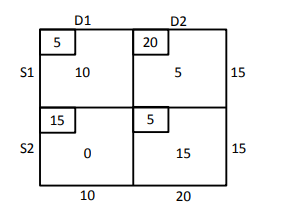
\includegraphics[width=0.75\columnwidth]{chapters/10/7/2/4/figs/fig.png}
 \end{center}
\caption{}
\label{fig:10/7/2/4Fig1}
\end{figure}
\fi

\item Find the position vector of the mid point of the vector joining the points $\vec{P}$(2, 3, 4)
and $\vec{Q}$(4, 1, –2).
\\
\solution
		\begin{enumerate}[label=\thesubsection.\arabic*,ref=\thesubsection.\theenumi]
\item Find the coordinates of the point which divides the join of $(-1,7) $ and $ (4,-3)$ in the ratio 2:3.
	\\
		\solution
	\input{chapters/10/7/2/1/section.tex}
\item Find the coordinates of the point $\vec{R}$ on the line segment joining the points $\vec{P}(-1,3)$ and $\vec{Q}(2,5)$ such that $PR=\frac{3}{5}PQ$.
\item Find the ratio in which the point $\vec{P}\brak{\frac{3}{4},\frac{5}{12}}$ divides the line segment joining the points $\vec{A}\brak{\frac{1}{2},\frac{3}{2}}$ and $ \vec{B}(2,-5)$.
\item Find the coordinates of the point which divides the line segment joining the points $(4,-3)$ and $(8,5)$ in the ratio $3:1$ internally.
\item Find the coordinates of the point $\vec{P}$ on $AD$ such that $AP : PD = 2 : 1$.
\item If the point $\vec{P} (2, 1)$ lies on the line segment joining points $\vec{A} (4, 2)$  and $ \vec{B} (8, 4)$,
then
\begin{enumerate}
	\item $AP =\frac{1}{3}{AB}$ 
\item ${AP}={PE}$
\item ${PB}=\frac{1}{3}{AB}$
\item${AP}=\frac{1}{2}{AB}$
 \end{enumerate}
\item Find the ratio in which the line segment joining the points $(-3,10)$  and  $(6,-8)$  is divided by $ (-1,6)$.
	\\
		\solution
	\input{chapters/10/7/2/4/section.tex}
\item Find the position vector of the mid point of the vector joining the points $\vec{P}$(2, 3, 4)
and $\vec{Q}$(4, 1, –2).
\\
\solution
		\input{chapters/12/10/2/16/section.tex}
\item Let $\vec{A}(4, 2), \vec{B}(6, 5)$  and $ \vec{C}(1, 4)$ be the vertices of $\triangle ABC$.
\begin{enumerate}
\item If $\vec{A}$ and  $\vec{B}$ are $(-2,-2)$ and  $(2,-4)$, respectively, find the coordinates of $\vec{P}$ such that $AP= \frac {3}{7}AB$  and $ \vec{P}$ lies on the line segment $AB$.
	\\
		\solution
	\input{chapters/10/7/2/8/section.tex}
\item Find the coordinates of the points which divide the line segment joining $A(-2,2)$  and  $\vec{B}(2,8)$ into four equal parts.
	\\
		\solution
	\input{chapters/10/7/2/9/section.tex}
\item In what ratio does the point $(-4,6)$ divide the line segment joining the points $\vec{A}(-6,0)$ and $\vec{B}(3,-8)$?
\item Given that $\vec{P}(3,2,-4), \vec{Q}(5,4,-6)$ and $\vec{R}(9,8,-10)$ are collinear. Find the ratio in which $\vec{Q}$ divides $PR$.
\item Points $\vec{A}(-6,10),\vec{B}(-4,6)$  and  $\vec{C}(3,-8)$ are collinear such that $AB=  \frac{2}{9}AC$.
\item The point which divides the line segment joining the points $\vec{P} (7, –6) $  and  $\vec{Q}(3, 4)$ in the 
ratio 1 : 2 internally lies in  which quadrant?
\item Find the coordinates of the points of trisection of the line segment joining $(4,-1)$  and  $(-2,3)$.
	\\
		\solution
	\input{chapters/10/7/2/2/section.tex}
\item Find the coordinates of the points which trisect the line segment joining the points $\vec{P}(4,2,-6)$ and $\vec{Q}(10,-16,6)$.
\item Find the coordinates of the points of trisection (i.e. points dividing to three equal parts) of the line segment joining the points $\vec{A}(2,-2)$ and $\vec{B}(-7,4)$.
\item Point $\vec{P}(5,-3)$ is one of the two points of trisection of line segment joining the points $\vec{A}(7,-2)$ and $\vec{B}(1,-5)$
\item Find the position vector of a point $\vec{R}$ which divides the line joining two points $\vec{P}$
and $\vec{Q}$ whose position vectors are $\hat{i}+2\hat{j}-\hat{k}$ and $-\hat{i}+\hat{j}+\hat{k}$ respectively, in the
ratio 2 : 1
\begin{enumerate}
    \item  internally
    \item  externally
\end{enumerate}
%\solution
%		\input{chapters/12/10/2/15/section.tex}
\item Find the coordinates of the point which divides the line segment joining the points which divides the line segment joining  the points $(-2,3,5)$ and $(1,-4,6)$ in the ratio 
\begin{enumerate}
\item $2:3$ internally,
\item $2:3$ externally
\end{enumerate}
\item Find the coordinates of the point which divides the line segment joining the points $(1,-2,3)$ and $(3,4,-5)$ in the ratio $2:3$
\begin{enumerate}
\item internally, and
\item externally
\end{enumerate}
\item Consider two points $\vec{P}$ and $\vec{Q}$ with position vectors $\overrightarrow{OP} = 3\overrightarrow{a}-2\overrightarrow{b}$ and $\overrightarrow{OQ}=\overrightarrow{a}+\overrightarrow{b}$. Find the position vector of a point $\vec{R}$ which divides the line joining $\vec{P}$ and $\vec{Q}$ in the ratio $2:1$, 
\begin{enumerate}
\item internally, and 
\item externally.
\end{enumerate}
\item The median from $\vec{A}$ meets $BC$ at $\vec{D}$. Find the coordinates of the point $\vec{D}$.
\item Find the coordinates of points $\vec{Q}$ and $\vec{R}$ on medians $BE$ and $CF$ respectively such that $BQ : QE = 2 : 1$  and  $CR : RF = 2 : 1$.
\item What do you observe?
\item If $\vec{A}, \vec{B}$ and $\vec{C}$  are the vertices of $\triangle ABC$, find the coordinates of the centroid of the triangle.
\end{enumerate}
\solution
	\input{chapters/10/7/4/7/section.tex}
\item If $\vec{P}(9a-2,-b)$ divides line segment joining $\vec{A}(3a+1,-3)$ and $\vec{B}(8a,5)$ in the ratio 3:1, find the values of $a$ and $b$.
\item Find the position vector of a point $\vec{R}$ which divides the line joining two points $\vec{P}$ and $\vec{Q}$ whose position vectors are $2\vec{a}+\vec{b}$ and $\vec{a}-3\vec{b}$ externally in the ratio $1:2$.
\item The position vector of the point which divides the join of points 2$\vec{a}$-3$\vec{b}$ $\text{and}$ $\vec{a}+\vec{b}$ in the ratio 3:1 is \rule{1cm}{0.1pt}.
\item If $\vec{a}$ and $\vec{b}$ are the postion vectors of $\vec{A}$ and $\vec{B}$, respectively, find the position vector of a point $\vec{C}$ in $BA$ produced such that $BC=1.5BA$.
\item Find the position vector of a point $\vec{R}$ which divides the line joining two points $\vec{P}$ and $\vec{Q}$ whose position vectors are $(2\vec{a}+\vec{b})$ and $(\vec{a}-3\vec{b})$
externally in the ratio 1 : 2. Also, show that $\vec{P}$ is the mid point of the line segment $RQ$.
\end{enumerate}

\item Let $\vec{A}(4, 2), \vec{B}(6, 5)$  and $ \vec{C}(1, 4)$ be the vertices of $\triangle ABC$.
\begin{enumerate}
\item If $\vec{A}$ and  $\vec{B}$ are $(-2,-2)$ and  $(2,-4)$, respectively, find the coordinates of $\vec{P}$ such that $AP= \frac {3}{7}AB$  and $ \vec{P}$ lies on the line segment $AB$.
	\\
		\solution
	\begin{enumerate}[label=\thesubsection.\arabic*,ref=\thesubsection.\theenumi]
\item Find the coordinates of the point which divides the join of $(-1,7) $ and $ (4,-3)$ in the ratio 2:3.
	\\
		\solution
	\input{chapters/10/7/2/1/section.tex}
\item Find the coordinates of the point $\vec{R}$ on the line segment joining the points $\vec{P}(-1,3)$ and $\vec{Q}(2,5)$ such that $PR=\frac{3}{5}PQ$.
\item Find the ratio in which the point $\vec{P}\brak{\frac{3}{4},\frac{5}{12}}$ divides the line segment joining the points $\vec{A}\brak{\frac{1}{2},\frac{3}{2}}$ and $ \vec{B}(2,-5)$.
\item Find the coordinates of the point which divides the line segment joining the points $(4,-3)$ and $(8,5)$ in the ratio $3:1$ internally.
\item Find the coordinates of the point $\vec{P}$ on $AD$ such that $AP : PD = 2 : 1$.
\item If the point $\vec{P} (2, 1)$ lies on the line segment joining points $\vec{A} (4, 2)$  and $ \vec{B} (8, 4)$,
then
\begin{enumerate}
	\item $AP =\frac{1}{3}{AB}$ 
\item ${AP}={PE}$
\item ${PB}=\frac{1}{3}{AB}$
\item${AP}=\frac{1}{2}{AB}$
 \end{enumerate}
\item Find the ratio in which the line segment joining the points $(-3,10)$  and  $(6,-8)$  is divided by $ (-1,6)$.
	\\
		\solution
	\input{chapters/10/7/2/4/section.tex}
\item Find the position vector of the mid point of the vector joining the points $\vec{P}$(2, 3, 4)
and $\vec{Q}$(4, 1, –2).
\\
\solution
		\input{chapters/12/10/2/16/section.tex}
\item Let $\vec{A}(4, 2), \vec{B}(6, 5)$  and $ \vec{C}(1, 4)$ be the vertices of $\triangle ABC$.
\begin{enumerate}
\item If $\vec{A}$ and  $\vec{B}$ are $(-2,-2)$ and  $(2,-4)$, respectively, find the coordinates of $\vec{P}$ such that $AP= \frac {3}{7}AB$  and $ \vec{P}$ lies on the line segment $AB$.
	\\
		\solution
	\input{chapters/10/7/2/8/section.tex}
\item Find the coordinates of the points which divide the line segment joining $A(-2,2)$  and  $\vec{B}(2,8)$ into four equal parts.
	\\
		\solution
	\input{chapters/10/7/2/9/section.tex}
\item In what ratio does the point $(-4,6)$ divide the line segment joining the points $\vec{A}(-6,0)$ and $\vec{B}(3,-8)$?
\item Given that $\vec{P}(3,2,-4), \vec{Q}(5,4,-6)$ and $\vec{R}(9,8,-10)$ are collinear. Find the ratio in which $\vec{Q}$ divides $PR$.
\item Points $\vec{A}(-6,10),\vec{B}(-4,6)$  and  $\vec{C}(3,-8)$ are collinear such that $AB=  \frac{2}{9}AC$.
\item The point which divides the line segment joining the points $\vec{P} (7, –6) $  and  $\vec{Q}(3, 4)$ in the 
ratio 1 : 2 internally lies in  which quadrant?
\item Find the coordinates of the points of trisection of the line segment joining $(4,-1)$  and  $(-2,3)$.
	\\
		\solution
	\input{chapters/10/7/2/2/section.tex}
\item Find the coordinates of the points which trisect the line segment joining the points $\vec{P}(4,2,-6)$ and $\vec{Q}(10,-16,6)$.
\item Find the coordinates of the points of trisection (i.e. points dividing to three equal parts) of the line segment joining the points $\vec{A}(2,-2)$ and $\vec{B}(-7,4)$.
\item Point $\vec{P}(5,-3)$ is one of the two points of trisection of line segment joining the points $\vec{A}(7,-2)$ and $\vec{B}(1,-5)$
\item Find the position vector of a point $\vec{R}$ which divides the line joining two points $\vec{P}$
and $\vec{Q}$ whose position vectors are $\hat{i}+2\hat{j}-\hat{k}$ and $-\hat{i}+\hat{j}+\hat{k}$ respectively, in the
ratio 2 : 1
\begin{enumerate}
    \item  internally
    \item  externally
\end{enumerate}
%\solution
%		\input{chapters/12/10/2/15/section.tex}
\item Find the coordinates of the point which divides the line segment joining the points which divides the line segment joining  the points $(-2,3,5)$ and $(1,-4,6)$ in the ratio 
\begin{enumerate}
\item $2:3$ internally,
\item $2:3$ externally
\end{enumerate}
\item Find the coordinates of the point which divides the line segment joining the points $(1,-2,3)$ and $(3,4,-5)$ in the ratio $2:3$
\begin{enumerate}
\item internally, and
\item externally
\end{enumerate}
\item Consider two points $\vec{P}$ and $\vec{Q}$ with position vectors $\overrightarrow{OP} = 3\overrightarrow{a}-2\overrightarrow{b}$ and $\overrightarrow{OQ}=\overrightarrow{a}+\overrightarrow{b}$. Find the position vector of a point $\vec{R}$ which divides the line joining $\vec{P}$ and $\vec{Q}$ in the ratio $2:1$, 
\begin{enumerate}
\item internally, and 
\item externally.
\end{enumerate}
\item The median from $\vec{A}$ meets $BC$ at $\vec{D}$. Find the coordinates of the point $\vec{D}$.
\item Find the coordinates of points $\vec{Q}$ and $\vec{R}$ on medians $BE$ and $CF$ respectively such that $BQ : QE = 2 : 1$  and  $CR : RF = 2 : 1$.
\item What do you observe?
\item If $\vec{A}, \vec{B}$ and $\vec{C}$  are the vertices of $\triangle ABC$, find the coordinates of the centroid of the triangle.
\end{enumerate}
\solution
	\input{chapters/10/7/4/7/section.tex}
\item If $\vec{P}(9a-2,-b)$ divides line segment joining $\vec{A}(3a+1,-3)$ and $\vec{B}(8a,5)$ in the ratio 3:1, find the values of $a$ and $b$.
\item Find the position vector of a point $\vec{R}$ which divides the line joining two points $\vec{P}$ and $\vec{Q}$ whose position vectors are $2\vec{a}+\vec{b}$ and $\vec{a}-3\vec{b}$ externally in the ratio $1:2$.
\item The position vector of the point which divides the join of points 2$\vec{a}$-3$\vec{b}$ $\text{and}$ $\vec{a}+\vec{b}$ in the ratio 3:1 is \rule{1cm}{0.1pt}.
\item If $\vec{a}$ and $\vec{b}$ are the postion vectors of $\vec{A}$ and $\vec{B}$, respectively, find the position vector of a point $\vec{C}$ in $BA$ produced such that $BC=1.5BA$.
\item Find the position vector of a point $\vec{R}$ which divides the line joining two points $\vec{P}$ and $\vec{Q}$ whose position vectors are $(2\vec{a}+\vec{b})$ and $(\vec{a}-3\vec{b})$
externally in the ratio 1 : 2. Also, show that $\vec{P}$ is the mid point of the line segment $RQ$.
\end{enumerate}

\item Find the coordinates of the points which divide the line segment joining $A(-2,2)$  and  $\vec{B}(2,8)$ into four equal parts.
	\\
		\solution
	\begin{enumerate}[label=\thesubsection.\arabic*,ref=\thesubsection.\theenumi]
\item Find the coordinates of the point which divides the join of $(-1,7) $ and $ (4,-3)$ in the ratio 2:3.
	\\
		\solution
	\input{chapters/10/7/2/1/section.tex}
\item Find the coordinates of the point $\vec{R}$ on the line segment joining the points $\vec{P}(-1,3)$ and $\vec{Q}(2,5)$ such that $PR=\frac{3}{5}PQ$.
\item Find the ratio in which the point $\vec{P}\brak{\frac{3}{4},\frac{5}{12}}$ divides the line segment joining the points $\vec{A}\brak{\frac{1}{2},\frac{3}{2}}$ and $ \vec{B}(2,-5)$.
\item Find the coordinates of the point which divides the line segment joining the points $(4,-3)$ and $(8,5)$ in the ratio $3:1$ internally.
\item Find the coordinates of the point $\vec{P}$ on $AD$ such that $AP : PD = 2 : 1$.
\item If the point $\vec{P} (2, 1)$ lies on the line segment joining points $\vec{A} (4, 2)$  and $ \vec{B} (8, 4)$,
then
\begin{enumerate}
	\item $AP =\frac{1}{3}{AB}$ 
\item ${AP}={PE}$
\item ${PB}=\frac{1}{3}{AB}$
\item${AP}=\frac{1}{2}{AB}$
 \end{enumerate}
\item Find the ratio in which the line segment joining the points $(-3,10)$  and  $(6,-8)$  is divided by $ (-1,6)$.
	\\
		\solution
	\input{chapters/10/7/2/4/section.tex}
\item Find the position vector of the mid point of the vector joining the points $\vec{P}$(2, 3, 4)
and $\vec{Q}$(4, 1, –2).
\\
\solution
		\input{chapters/12/10/2/16/section.tex}
\item Let $\vec{A}(4, 2), \vec{B}(6, 5)$  and $ \vec{C}(1, 4)$ be the vertices of $\triangle ABC$.
\begin{enumerate}
\item If $\vec{A}$ and  $\vec{B}$ are $(-2,-2)$ and  $(2,-4)$, respectively, find the coordinates of $\vec{P}$ such that $AP= \frac {3}{7}AB$  and $ \vec{P}$ lies on the line segment $AB$.
	\\
		\solution
	\input{chapters/10/7/2/8/section.tex}
\item Find the coordinates of the points which divide the line segment joining $A(-2,2)$  and  $\vec{B}(2,8)$ into four equal parts.
	\\
		\solution
	\input{chapters/10/7/2/9/section.tex}
\item In what ratio does the point $(-4,6)$ divide the line segment joining the points $\vec{A}(-6,0)$ and $\vec{B}(3,-8)$?
\item Given that $\vec{P}(3,2,-4), \vec{Q}(5,4,-6)$ and $\vec{R}(9,8,-10)$ are collinear. Find the ratio in which $\vec{Q}$ divides $PR$.
\item Points $\vec{A}(-6,10),\vec{B}(-4,6)$  and  $\vec{C}(3,-8)$ are collinear such that $AB=  \frac{2}{9}AC$.
\item The point which divides the line segment joining the points $\vec{P} (7, –6) $  and  $\vec{Q}(3, 4)$ in the 
ratio 1 : 2 internally lies in  which quadrant?
\item Find the coordinates of the points of trisection of the line segment joining $(4,-1)$  and  $(-2,3)$.
	\\
		\solution
	\input{chapters/10/7/2/2/section.tex}
\item Find the coordinates of the points which trisect the line segment joining the points $\vec{P}(4,2,-6)$ and $\vec{Q}(10,-16,6)$.
\item Find the coordinates of the points of trisection (i.e. points dividing to three equal parts) of the line segment joining the points $\vec{A}(2,-2)$ and $\vec{B}(-7,4)$.
\item Point $\vec{P}(5,-3)$ is one of the two points of trisection of line segment joining the points $\vec{A}(7,-2)$ and $\vec{B}(1,-5)$
\item Find the position vector of a point $\vec{R}$ which divides the line joining two points $\vec{P}$
and $\vec{Q}$ whose position vectors are $\hat{i}+2\hat{j}-\hat{k}$ and $-\hat{i}+\hat{j}+\hat{k}$ respectively, in the
ratio 2 : 1
\begin{enumerate}
    \item  internally
    \item  externally
\end{enumerate}
%\solution
%		\input{chapters/12/10/2/15/section.tex}
\item Find the coordinates of the point which divides the line segment joining the points which divides the line segment joining  the points $(-2,3,5)$ and $(1,-4,6)$ in the ratio 
\begin{enumerate}
\item $2:3$ internally,
\item $2:3$ externally
\end{enumerate}
\item Find the coordinates of the point which divides the line segment joining the points $(1,-2,3)$ and $(3,4,-5)$ in the ratio $2:3$
\begin{enumerate}
\item internally, and
\item externally
\end{enumerate}
\item Consider two points $\vec{P}$ and $\vec{Q}$ with position vectors $\overrightarrow{OP} = 3\overrightarrow{a}-2\overrightarrow{b}$ and $\overrightarrow{OQ}=\overrightarrow{a}+\overrightarrow{b}$. Find the position vector of a point $\vec{R}$ which divides the line joining $\vec{P}$ and $\vec{Q}$ in the ratio $2:1$, 
\begin{enumerate}
\item internally, and 
\item externally.
\end{enumerate}
\item The median from $\vec{A}$ meets $BC$ at $\vec{D}$. Find the coordinates of the point $\vec{D}$.
\item Find the coordinates of points $\vec{Q}$ and $\vec{R}$ on medians $BE$ and $CF$ respectively such that $BQ : QE = 2 : 1$  and  $CR : RF = 2 : 1$.
\item What do you observe?
\item If $\vec{A}, \vec{B}$ and $\vec{C}$  are the vertices of $\triangle ABC$, find the coordinates of the centroid of the triangle.
\end{enumerate}
\solution
	\input{chapters/10/7/4/7/section.tex}
\item If $\vec{P}(9a-2,-b)$ divides line segment joining $\vec{A}(3a+1,-3)$ and $\vec{B}(8a,5)$ in the ratio 3:1, find the values of $a$ and $b$.
\item Find the position vector of a point $\vec{R}$ which divides the line joining two points $\vec{P}$ and $\vec{Q}$ whose position vectors are $2\vec{a}+\vec{b}$ and $\vec{a}-3\vec{b}$ externally in the ratio $1:2$.
\item The position vector of the point which divides the join of points 2$\vec{a}$-3$\vec{b}$ $\text{and}$ $\vec{a}+\vec{b}$ in the ratio 3:1 is \rule{1cm}{0.1pt}.
\item If $\vec{a}$ and $\vec{b}$ are the postion vectors of $\vec{A}$ and $\vec{B}$, respectively, find the position vector of a point $\vec{C}$ in $BA$ produced such that $BC=1.5BA$.
\item Find the position vector of a point $\vec{R}$ which divides the line joining two points $\vec{P}$ and $\vec{Q}$ whose position vectors are $(2\vec{a}+\vec{b})$ and $(\vec{a}-3\vec{b})$
externally in the ratio 1 : 2. Also, show that $\vec{P}$ is the mid point of the line segment $RQ$.
\end{enumerate}

\item In what ratio does the point $(-4,6)$ divide the line segment joining the points $\vec{A}(-6,0)$ and $\vec{B}(3,-8)$?
\item Given that $\vec{P}(3,2,-4), \vec{Q}(5,4,-6)$ and $\vec{R}(9,8,-10)$ are collinear. Find the ratio in which $\vec{Q}$ divides $PR$.
\item Points $\vec{A}(-6,10),\vec{B}(-4,6)$  and  $\vec{C}(3,-8)$ are collinear such that $AB=  \frac{2}{9}AC$.
\item The point which divides the line segment joining the points $\vec{P} (7, –6) $  and  $\vec{Q}(3, 4)$ in the 
ratio 1 : 2 internally lies in  which quadrant?
\item Find the coordinates of the points of trisection of the line segment joining $(4,-1)$  and  $(-2,3)$.
	\\
		\solution
	Using section formula,
\begin{align}
\vec{R}=\frac{1}{1+\frac{1}{2}}\brak{\myvec{4\\-1}+\frac{1}{2}\myvec{-2\\3}}
=\myvec{2\\ \frac{1}{3}}\\
\vec{S}=\frac{1}{1+\frac{2}{1}}\brak{\myvec{4\\-1}+\frac{2}{1}\myvec{-2\\3}}
=\myvec{0\\ \frac{5}{3}}
\end{align}
which are the desired points of trisection.
\iffalse
See
		\figref{fig:chapters/10/7/2/2/Figure}
\begin{figure}[H]
\centering
\includegraphics[width=0.75\columnwidth]{chapters/10/7/2/2/figs/dj.pdf}
\caption{}
		\label{fig:chapters/10/7/2/2/Figure}
\end{figure}
\fi

\item Find the coordinates of the points which trisect the line segment joining the points $\vec{P}(4,2,-6)$ and $\vec{Q}(10,-16,6)$.
\item Find the coordinates of the points of trisection (i.e. points dividing to three equal parts) of the line segment joining the points $\vec{A}(2,-2)$ and $\vec{B}(-7,4)$.
\item Point $\vec{P}(5,-3)$ is one of the two points of trisection of line segment joining the points $\vec{A}(7,-2)$ and $\vec{B}(1,-5)$
\item Find the position vector of a point $\vec{R}$ which divides the line joining two points $\vec{P}$
and $\vec{Q}$ whose position vectors are $\hat{i}+2\hat{j}-\hat{k}$ and $-\hat{i}+\hat{j}+\hat{k}$ respectively, in the
ratio 2 : 1
\begin{enumerate}
    \item  internally
    \item  externally
\end{enumerate}
%\solution
%		\begin{enumerate}[label=\thesubsection.\arabic*,ref=\thesubsection.\theenumi]
\item Find the coordinates of the point which divides the join of $(-1,7) $ and $ (4,-3)$ in the ratio 2:3.
	\\
		\solution
	\input{chapters/10/7/2/1/section.tex}
\item Find the coordinates of the point $\vec{R}$ on the line segment joining the points $\vec{P}(-1,3)$ and $\vec{Q}(2,5)$ such that $PR=\frac{3}{5}PQ$.
\item Find the ratio in which the point $\vec{P}\brak{\frac{3}{4},\frac{5}{12}}$ divides the line segment joining the points $\vec{A}\brak{\frac{1}{2},\frac{3}{2}}$ and $ \vec{B}(2,-5)$.
\item Find the coordinates of the point which divides the line segment joining the points $(4,-3)$ and $(8,5)$ in the ratio $3:1$ internally.
\item Find the coordinates of the point $\vec{P}$ on $AD$ such that $AP : PD = 2 : 1$.
\item If the point $\vec{P} (2, 1)$ lies on the line segment joining points $\vec{A} (4, 2)$  and $ \vec{B} (8, 4)$,
then
\begin{enumerate}
	\item $AP =\frac{1}{3}{AB}$ 
\item ${AP}={PE}$
\item ${PB}=\frac{1}{3}{AB}$
\item${AP}=\frac{1}{2}{AB}$
 \end{enumerate}
\item Find the ratio in which the line segment joining the points $(-3,10)$  and  $(6,-8)$  is divided by $ (-1,6)$.
	\\
		\solution
	\input{chapters/10/7/2/4/section.tex}
\item Find the position vector of the mid point of the vector joining the points $\vec{P}$(2, 3, 4)
and $\vec{Q}$(4, 1, –2).
\\
\solution
		\input{chapters/12/10/2/16/section.tex}
\item Let $\vec{A}(4, 2), \vec{B}(6, 5)$  and $ \vec{C}(1, 4)$ be the vertices of $\triangle ABC$.
\begin{enumerate}
\item If $\vec{A}$ and  $\vec{B}$ are $(-2,-2)$ and  $(2,-4)$, respectively, find the coordinates of $\vec{P}$ such that $AP= \frac {3}{7}AB$  and $ \vec{P}$ lies on the line segment $AB$.
	\\
		\solution
	\input{chapters/10/7/2/8/section.tex}
\item Find the coordinates of the points which divide the line segment joining $A(-2,2)$  and  $\vec{B}(2,8)$ into four equal parts.
	\\
		\solution
	\input{chapters/10/7/2/9/section.tex}
\item In what ratio does the point $(-4,6)$ divide the line segment joining the points $\vec{A}(-6,0)$ and $\vec{B}(3,-8)$?
\item Given that $\vec{P}(3,2,-4), \vec{Q}(5,4,-6)$ and $\vec{R}(9,8,-10)$ are collinear. Find the ratio in which $\vec{Q}$ divides $PR$.
\item Points $\vec{A}(-6,10),\vec{B}(-4,6)$  and  $\vec{C}(3,-8)$ are collinear such that $AB=  \frac{2}{9}AC$.
\item The point which divides the line segment joining the points $\vec{P} (7, –6) $  and  $\vec{Q}(3, 4)$ in the 
ratio 1 : 2 internally lies in  which quadrant?
\item Find the coordinates of the points of trisection of the line segment joining $(4,-1)$  and  $(-2,3)$.
	\\
		\solution
	\input{chapters/10/7/2/2/section.tex}
\item Find the coordinates of the points which trisect the line segment joining the points $\vec{P}(4,2,-6)$ and $\vec{Q}(10,-16,6)$.
\item Find the coordinates of the points of trisection (i.e. points dividing to three equal parts) of the line segment joining the points $\vec{A}(2,-2)$ and $\vec{B}(-7,4)$.
\item Point $\vec{P}(5,-3)$ is one of the two points of trisection of line segment joining the points $\vec{A}(7,-2)$ and $\vec{B}(1,-5)$
\item Find the position vector of a point $\vec{R}$ which divides the line joining two points $\vec{P}$
and $\vec{Q}$ whose position vectors are $\hat{i}+2\hat{j}-\hat{k}$ and $-\hat{i}+\hat{j}+\hat{k}$ respectively, in the
ratio 2 : 1
\begin{enumerate}
    \item  internally
    \item  externally
\end{enumerate}
%\solution
%		\input{chapters/12/10/2/15/section.tex}
\item Find the coordinates of the point which divides the line segment joining the points which divides the line segment joining  the points $(-2,3,5)$ and $(1,-4,6)$ in the ratio 
\begin{enumerate}
\item $2:3$ internally,
\item $2:3$ externally
\end{enumerate}
\item Find the coordinates of the point which divides the line segment joining the points $(1,-2,3)$ and $(3,4,-5)$ in the ratio $2:3$
\begin{enumerate}
\item internally, and
\item externally
\end{enumerate}
\item Consider two points $\vec{P}$ and $\vec{Q}$ with position vectors $\overrightarrow{OP} = 3\overrightarrow{a}-2\overrightarrow{b}$ and $\overrightarrow{OQ}=\overrightarrow{a}+\overrightarrow{b}$. Find the position vector of a point $\vec{R}$ which divides the line joining $\vec{P}$ and $\vec{Q}$ in the ratio $2:1$, 
\begin{enumerate}
\item internally, and 
\item externally.
\end{enumerate}
\item The median from $\vec{A}$ meets $BC$ at $\vec{D}$. Find the coordinates of the point $\vec{D}$.
\item Find the coordinates of points $\vec{Q}$ and $\vec{R}$ on medians $BE$ and $CF$ respectively such that $BQ : QE = 2 : 1$  and  $CR : RF = 2 : 1$.
\item What do you observe?
\item If $\vec{A}, \vec{B}$ and $\vec{C}$  are the vertices of $\triangle ABC$, find the coordinates of the centroid of the triangle.
\end{enumerate}
\solution
	\input{chapters/10/7/4/7/section.tex}
\item If $\vec{P}(9a-2,-b)$ divides line segment joining $\vec{A}(3a+1,-3)$ and $\vec{B}(8a,5)$ in the ratio 3:1, find the values of $a$ and $b$.
\item Find the position vector of a point $\vec{R}$ which divides the line joining two points $\vec{P}$ and $\vec{Q}$ whose position vectors are $2\vec{a}+\vec{b}$ and $\vec{a}-3\vec{b}$ externally in the ratio $1:2$.
\item The position vector of the point which divides the join of points 2$\vec{a}$-3$\vec{b}$ $\text{and}$ $\vec{a}+\vec{b}$ in the ratio 3:1 is \rule{1cm}{0.1pt}.
\item If $\vec{a}$ and $\vec{b}$ are the postion vectors of $\vec{A}$ and $\vec{B}$, respectively, find the position vector of a point $\vec{C}$ in $BA$ produced such that $BC=1.5BA$.
\item Find the position vector of a point $\vec{R}$ which divides the line joining two points $\vec{P}$ and $\vec{Q}$ whose position vectors are $(2\vec{a}+\vec{b})$ and $(\vec{a}-3\vec{b})$
externally in the ratio 1 : 2. Also, show that $\vec{P}$ is the mid point of the line segment $RQ$.
\end{enumerate}

\item Find the coordinates of the point which divides the line segment joining the points which divides the line segment joining  the points $(-2,3,5)$ and $(1,-4,6)$ in the ratio 
\begin{enumerate}
\item $2:3$ internally,
\item $2:3$ externally
\end{enumerate}
\item Find the coordinates of the point which divides the line segment joining the points $(1,-2,3)$ and $(3,4,-5)$ in the ratio $2:3$
\begin{enumerate}
\item internally, and
\item externally
\end{enumerate}
\item Consider two points $\vec{P}$ and $\vec{Q}$ with position vectors $\overrightarrow{OP} = 3\overrightarrow{a}-2\overrightarrow{b}$ and $\overrightarrow{OQ}=\overrightarrow{a}+\overrightarrow{b}$. Find the position vector of a point $\vec{R}$ which divides the line joining $\vec{P}$ and $\vec{Q}$ in the ratio $2:1$, 
\begin{enumerate}
\item internally, and 
\item externally.
\end{enumerate}
\item The median from $\vec{A}$ meets $BC$ at $\vec{D}$. Find the coordinates of the point $\vec{D}$.
\item Find the coordinates of points $\vec{Q}$ and $\vec{R}$ on medians $BE$ and $CF$ respectively such that $BQ : QE = 2 : 1$  and  $CR : RF = 2 : 1$.
\item What do you observe?
\item If $\vec{A}, \vec{B}$ and $\vec{C}$  are the vertices of $\triangle ABC$, find the coordinates of the centroid of the triangle.
\end{enumerate}
\solution
	\begin{enumerate}[label=\thesubsection.\arabic*,ref=\thesubsection.\theenumi]
\item Find the coordinates of the point which divides the join of $(-1,7) $ and $ (4,-3)$ in the ratio 2:3.
	\\
		\solution
	\input{chapters/10/7/2/1/section.tex}
\item Find the coordinates of the point $\vec{R}$ on the line segment joining the points $\vec{P}(-1,3)$ and $\vec{Q}(2,5)$ such that $PR=\frac{3}{5}PQ$.
\item Find the ratio in which the point $\vec{P}\brak{\frac{3}{4},\frac{5}{12}}$ divides the line segment joining the points $\vec{A}\brak{\frac{1}{2},\frac{3}{2}}$ and $ \vec{B}(2,-5)$.
\item Find the coordinates of the point which divides the line segment joining the points $(4,-3)$ and $(8,5)$ in the ratio $3:1$ internally.
\item Find the coordinates of the point $\vec{P}$ on $AD$ such that $AP : PD = 2 : 1$.
\item If the point $\vec{P} (2, 1)$ lies on the line segment joining points $\vec{A} (4, 2)$  and $ \vec{B} (8, 4)$,
then
\begin{enumerate}
	\item $AP =\frac{1}{3}{AB}$ 
\item ${AP}={PE}$
\item ${PB}=\frac{1}{3}{AB}$
\item${AP}=\frac{1}{2}{AB}$
 \end{enumerate}
\item Find the ratio in which the line segment joining the points $(-3,10)$  and  $(6,-8)$  is divided by $ (-1,6)$.
	\\
		\solution
	\input{chapters/10/7/2/4/section.tex}
\item Find the position vector of the mid point of the vector joining the points $\vec{P}$(2, 3, 4)
and $\vec{Q}$(4, 1, –2).
\\
\solution
		\input{chapters/12/10/2/16/section.tex}
\item Let $\vec{A}(4, 2), \vec{B}(6, 5)$  and $ \vec{C}(1, 4)$ be the vertices of $\triangle ABC$.
\begin{enumerate}
\item If $\vec{A}$ and  $\vec{B}$ are $(-2,-2)$ and  $(2,-4)$, respectively, find the coordinates of $\vec{P}$ such that $AP= \frac {3}{7}AB$  and $ \vec{P}$ lies on the line segment $AB$.
	\\
		\solution
	\input{chapters/10/7/2/8/section.tex}
\item Find the coordinates of the points which divide the line segment joining $A(-2,2)$  and  $\vec{B}(2,8)$ into four equal parts.
	\\
		\solution
	\input{chapters/10/7/2/9/section.tex}
\item In what ratio does the point $(-4,6)$ divide the line segment joining the points $\vec{A}(-6,0)$ and $\vec{B}(3,-8)$?
\item Given that $\vec{P}(3,2,-4), \vec{Q}(5,4,-6)$ and $\vec{R}(9,8,-10)$ are collinear. Find the ratio in which $\vec{Q}$ divides $PR$.
\item Points $\vec{A}(-6,10),\vec{B}(-4,6)$  and  $\vec{C}(3,-8)$ are collinear such that $AB=  \frac{2}{9}AC$.
\item The point which divides the line segment joining the points $\vec{P} (7, –6) $  and  $\vec{Q}(3, 4)$ in the 
ratio 1 : 2 internally lies in  which quadrant?
\item Find the coordinates of the points of trisection of the line segment joining $(4,-1)$  and  $(-2,3)$.
	\\
		\solution
	\input{chapters/10/7/2/2/section.tex}
\item Find the coordinates of the points which trisect the line segment joining the points $\vec{P}(4,2,-6)$ and $\vec{Q}(10,-16,6)$.
\item Find the coordinates of the points of trisection (i.e. points dividing to three equal parts) of the line segment joining the points $\vec{A}(2,-2)$ and $\vec{B}(-7,4)$.
\item Point $\vec{P}(5,-3)$ is one of the two points of trisection of line segment joining the points $\vec{A}(7,-2)$ and $\vec{B}(1,-5)$
\item Find the position vector of a point $\vec{R}$ which divides the line joining two points $\vec{P}$
and $\vec{Q}$ whose position vectors are $\hat{i}+2\hat{j}-\hat{k}$ and $-\hat{i}+\hat{j}+\hat{k}$ respectively, in the
ratio 2 : 1
\begin{enumerate}
    \item  internally
    \item  externally
\end{enumerate}
%\solution
%		\input{chapters/12/10/2/15/section.tex}
\item Find the coordinates of the point which divides the line segment joining the points which divides the line segment joining  the points $(-2,3,5)$ and $(1,-4,6)$ in the ratio 
\begin{enumerate}
\item $2:3$ internally,
\item $2:3$ externally
\end{enumerate}
\item Find the coordinates of the point which divides the line segment joining the points $(1,-2,3)$ and $(3,4,-5)$ in the ratio $2:3$
\begin{enumerate}
\item internally, and
\item externally
\end{enumerate}
\item Consider two points $\vec{P}$ and $\vec{Q}$ with position vectors $\overrightarrow{OP} = 3\overrightarrow{a}-2\overrightarrow{b}$ and $\overrightarrow{OQ}=\overrightarrow{a}+\overrightarrow{b}$. Find the position vector of a point $\vec{R}$ which divides the line joining $\vec{P}$ and $\vec{Q}$ in the ratio $2:1$, 
\begin{enumerate}
\item internally, and 
\item externally.
\end{enumerate}
\item The median from $\vec{A}$ meets $BC$ at $\vec{D}$. Find the coordinates of the point $\vec{D}$.
\item Find the coordinates of points $\vec{Q}$ and $\vec{R}$ on medians $BE$ and $CF$ respectively such that $BQ : QE = 2 : 1$  and  $CR : RF = 2 : 1$.
\item What do you observe?
\item If $\vec{A}, \vec{B}$ and $\vec{C}$  are the vertices of $\triangle ABC$, find the coordinates of the centroid of the triangle.
\end{enumerate}
\solution
	\input{chapters/10/7/4/7/section.tex}
\item If $\vec{P}(9a-2,-b)$ divides line segment joining $\vec{A}(3a+1,-3)$ and $\vec{B}(8a,5)$ in the ratio 3:1, find the values of $a$ and $b$.
\item Find the position vector of a point $\vec{R}$ which divides the line joining two points $\vec{P}$ and $\vec{Q}$ whose position vectors are $2\vec{a}+\vec{b}$ and $\vec{a}-3\vec{b}$ externally in the ratio $1:2$.
\item The position vector of the point which divides the join of points 2$\vec{a}$-3$\vec{b}$ $\text{and}$ $\vec{a}+\vec{b}$ in the ratio 3:1 is \rule{1cm}{0.1pt}.
\item If $\vec{a}$ and $\vec{b}$ are the postion vectors of $\vec{A}$ and $\vec{B}$, respectively, find the position vector of a point $\vec{C}$ in $BA$ produced such that $BC=1.5BA$.
\item Find the position vector of a point $\vec{R}$ which divides the line joining two points $\vec{P}$ and $\vec{Q}$ whose position vectors are $(2\vec{a}+\vec{b})$ and $(\vec{a}-3\vec{b})$
externally in the ratio 1 : 2. Also, show that $\vec{P}$ is the mid point of the line segment $RQ$.
\end{enumerate}

\item If $\vec{P}(9a-2,-b)$ divides line segment joining $\vec{A}(3a+1,-3)$ and $\vec{B}(8a,5)$ in the ratio 3:1, find the values of $a$ and $b$.
\item Find the position vector of a point $\vec{R}$ which divides the line joining two points $\vec{P}$ and $\vec{Q}$ whose position vectors are $2\vec{a}+\vec{b}$ and $\vec{a}-3\vec{b}$ externally in the ratio $1:2$.
\item The position vector of the point which divides the join of points 2$\vec{a}$-3$\vec{b}$ $\text{and}$ $\vec{a}+\vec{b}$ in the ratio 3:1 is \rule{1cm}{0.1pt}.
\item If $\vec{a}$ and $\vec{b}$ are the postion vectors of $\vec{A}$ and $\vec{B}$, respectively, find the position vector of a point $\vec{C}$ in $BA$ produced such that $BC=1.5BA$.
\item Find the position vector of a point $\vec{R}$ which divides the line joining two points $\vec{P}$ and $\vec{Q}$ whose position vectors are $(2\vec{a}+\vec{b})$ and $(\vec{a}-3\vec{b})$
externally in the ratio 1 : 2. Also, show that $\vec{P}$ is the mid point of the line segment $RQ$.
\end{enumerate}

\item Let $\vec{A}(4, 2), \vec{B}(6, 5)$  and $ \vec{C}(1, 4)$ be the vertices of $\triangle ABC$.
\begin{enumerate}
\item If $\vec{A}$ and  $\vec{B}$ are $(-2,-2)$ and  $(2,-4)$, respectively, find the coordinates of $\vec{P}$ such that $AP= \frac {3}{7}AB$  and $ \vec{P}$ lies on the line segment $AB$.
	\\
		\solution
	\begin{enumerate}[label=\thesubsection.\arabic*,ref=\thesubsection.\theenumi]
\item Find the coordinates of the point which divides the join of $(-1,7) $ and $ (4,-3)$ in the ratio 2:3.
	\\
		\solution
	\begin{enumerate}[label=\thesubsection.\arabic*,ref=\thesubsection.\theenumi]
\item Find the coordinates of the point which divides the join of $(-1,7) $ and $ (4,-3)$ in the ratio 2:3.
	\\
		\solution
	\input{chapters/10/7/2/1/section.tex}
\item Find the coordinates of the point $\vec{R}$ on the line segment joining the points $\vec{P}(-1,3)$ and $\vec{Q}(2,5)$ such that $PR=\frac{3}{5}PQ$.
\item Find the ratio in which the point $\vec{P}\brak{\frac{3}{4},\frac{5}{12}}$ divides the line segment joining the points $\vec{A}\brak{\frac{1}{2},\frac{3}{2}}$ and $ \vec{B}(2,-5)$.
\item Find the coordinates of the point which divides the line segment joining the points $(4,-3)$ and $(8,5)$ in the ratio $3:1$ internally.
\item Find the coordinates of the point $\vec{P}$ on $AD$ such that $AP : PD = 2 : 1$.
\item If the point $\vec{P} (2, 1)$ lies on the line segment joining points $\vec{A} (4, 2)$  and $ \vec{B} (8, 4)$,
then
\begin{enumerate}
	\item $AP =\frac{1}{3}{AB}$ 
\item ${AP}={PE}$
\item ${PB}=\frac{1}{3}{AB}$
\item${AP}=\frac{1}{2}{AB}$
 \end{enumerate}
\item Find the ratio in which the line segment joining the points $(-3,10)$  and  $(6,-8)$  is divided by $ (-1,6)$.
	\\
		\solution
	\input{chapters/10/7/2/4/section.tex}
\item Find the position vector of the mid point of the vector joining the points $\vec{P}$(2, 3, 4)
and $\vec{Q}$(4, 1, –2).
\\
\solution
		\input{chapters/12/10/2/16/section.tex}
\item Let $\vec{A}(4, 2), \vec{B}(6, 5)$  and $ \vec{C}(1, 4)$ be the vertices of $\triangle ABC$.
\begin{enumerate}
\item If $\vec{A}$ and  $\vec{B}$ are $(-2,-2)$ and  $(2,-4)$, respectively, find the coordinates of $\vec{P}$ such that $AP= \frac {3}{7}AB$  and $ \vec{P}$ lies on the line segment $AB$.
	\\
		\solution
	\input{chapters/10/7/2/8/section.tex}
\item Find the coordinates of the points which divide the line segment joining $A(-2,2)$  and  $\vec{B}(2,8)$ into four equal parts.
	\\
		\solution
	\input{chapters/10/7/2/9/section.tex}
\item In what ratio does the point $(-4,6)$ divide the line segment joining the points $\vec{A}(-6,0)$ and $\vec{B}(3,-8)$?
\item Given that $\vec{P}(3,2,-4), \vec{Q}(5,4,-6)$ and $\vec{R}(9,8,-10)$ are collinear. Find the ratio in which $\vec{Q}$ divides $PR$.
\item Points $\vec{A}(-6,10),\vec{B}(-4,6)$  and  $\vec{C}(3,-8)$ are collinear such that $AB=  \frac{2}{9}AC$.
\item The point which divides the line segment joining the points $\vec{P} (7, –6) $  and  $\vec{Q}(3, 4)$ in the 
ratio 1 : 2 internally lies in  which quadrant?
\item Find the coordinates of the points of trisection of the line segment joining $(4,-1)$  and  $(-2,3)$.
	\\
		\solution
	\input{chapters/10/7/2/2/section.tex}
\item Find the coordinates of the points which trisect the line segment joining the points $\vec{P}(4,2,-6)$ and $\vec{Q}(10,-16,6)$.
\item Find the coordinates of the points of trisection (i.e. points dividing to three equal parts) of the line segment joining the points $\vec{A}(2,-2)$ and $\vec{B}(-7,4)$.
\item Point $\vec{P}(5,-3)$ is one of the two points of trisection of line segment joining the points $\vec{A}(7,-2)$ and $\vec{B}(1,-5)$
\item Find the position vector of a point $\vec{R}$ which divides the line joining two points $\vec{P}$
and $\vec{Q}$ whose position vectors are $\hat{i}+2\hat{j}-\hat{k}$ and $-\hat{i}+\hat{j}+\hat{k}$ respectively, in the
ratio 2 : 1
\begin{enumerate}
    \item  internally
    \item  externally
\end{enumerate}
%\solution
%		\input{chapters/12/10/2/15/section.tex}
\item Find the coordinates of the point which divides the line segment joining the points which divides the line segment joining  the points $(-2,3,5)$ and $(1,-4,6)$ in the ratio 
\begin{enumerate}
\item $2:3$ internally,
\item $2:3$ externally
\end{enumerate}
\item Find the coordinates of the point which divides the line segment joining the points $(1,-2,3)$ and $(3,4,-5)$ in the ratio $2:3$
\begin{enumerate}
\item internally, and
\item externally
\end{enumerate}
\item Consider two points $\vec{P}$ and $\vec{Q}$ with position vectors $\overrightarrow{OP} = 3\overrightarrow{a}-2\overrightarrow{b}$ and $\overrightarrow{OQ}=\overrightarrow{a}+\overrightarrow{b}$. Find the position vector of a point $\vec{R}$ which divides the line joining $\vec{P}$ and $\vec{Q}$ in the ratio $2:1$, 
\begin{enumerate}
\item internally, and 
\item externally.
\end{enumerate}
\item The median from $\vec{A}$ meets $BC$ at $\vec{D}$. Find the coordinates of the point $\vec{D}$.
\item Find the coordinates of points $\vec{Q}$ and $\vec{R}$ on medians $BE$ and $CF$ respectively such that $BQ : QE = 2 : 1$  and  $CR : RF = 2 : 1$.
\item What do you observe?
\item If $\vec{A}, \vec{B}$ and $\vec{C}$  are the vertices of $\triangle ABC$, find the coordinates of the centroid of the triangle.
\end{enumerate}
\solution
	\input{chapters/10/7/4/7/section.tex}
\item If $\vec{P}(9a-2,-b)$ divides line segment joining $\vec{A}(3a+1,-3)$ and $\vec{B}(8a,5)$ in the ratio 3:1, find the values of $a$ and $b$.
\item Find the position vector of a point $\vec{R}$ which divides the line joining two points $\vec{P}$ and $\vec{Q}$ whose position vectors are $2\vec{a}+\vec{b}$ and $\vec{a}-3\vec{b}$ externally in the ratio $1:2$.
\item The position vector of the point which divides the join of points 2$\vec{a}$-3$\vec{b}$ $\text{and}$ $\vec{a}+\vec{b}$ in the ratio 3:1 is \rule{1cm}{0.1pt}.
\item If $\vec{a}$ and $\vec{b}$ are the postion vectors of $\vec{A}$ and $\vec{B}$, respectively, find the position vector of a point $\vec{C}$ in $BA$ produced such that $BC=1.5BA$.
\item Find the position vector of a point $\vec{R}$ which divides the line joining two points $\vec{P}$ and $\vec{Q}$ whose position vectors are $(2\vec{a}+\vec{b})$ and $(\vec{a}-3\vec{b})$
externally in the ratio 1 : 2. Also, show that $\vec{P}$ is the mid point of the line segment $RQ$.
\end{enumerate}

\item Find the coordinates of the point $\vec{R}$ on the line segment joining the points $\vec{P}(-1,3)$ and $\vec{Q}(2,5)$ such that $PR=\frac{3}{5}PQ$.
\item Find the ratio in which the point $\vec{P}\brak{\frac{3}{4},\frac{5}{12}}$ divides the line segment joining the points $\vec{A}\brak{\frac{1}{2},\frac{3}{2}}$ and $ \vec{B}(2,-5)$.
\item Find the coordinates of the point which divides the line segment joining the points $(4,-3)$ and $(8,5)$ in the ratio $3:1$ internally.
\item Find the coordinates of the point $\vec{P}$ on $AD$ such that $AP : PD = 2 : 1$.
\item If the point $\vec{P} (2, 1)$ lies on the line segment joining points $\vec{A} (4, 2)$  and $ \vec{B} (8, 4)$,
then
\begin{enumerate}
	\item $AP =\frac{1}{3}{AB}$ 
\item ${AP}={PE}$
\item ${PB}=\frac{1}{3}{AB}$
\item${AP}=\frac{1}{2}{AB}$
 \end{enumerate}
\item Find the ratio in which the line segment joining the points $(-3,10)$  and  $(6,-8)$  is divided by $ (-1,6)$.
	\\
		\solution
	\iffalse
Using section formula,
\begin{align}
         \myvec{-1\\6} &=\frac{{\myvec{-3\\10}+k\myvec{6\\-8}}}{1+k}\\
	 \implies 7k\myvec{1 \\ -2} &= 2\myvec{1 \\ -2}
	 \\
	 \text{or, } k &= \frac{2}{7}.
\end{align}
\fi
In 
			\eqref{eq:section_formula-k}, substituting
			\begin{align}
				\vec{B} &= \myvec{-3\\10}, \vec{C} = \myvec{6\\-8}, \vec{D} = \myvec{-1\\6},
				\\
				k &= \frac{\myvec{-2 & 4}\myvec{-7 \\ 14}}{\norm{\myvec{-7 \\ 14}}^2} = \frac{2}{7}
			\end{align}
\iffalse
See \figref{fig:10/7/2/4Fig1}.
\begin{figure}[H]
 \begin{center}
  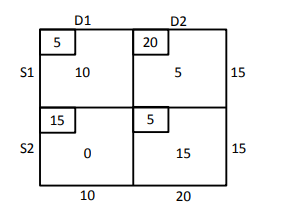
\includegraphics[width=0.75\columnwidth]{chapters/10/7/2/4/figs/fig.png}
 \end{center}
\caption{}
\label{fig:10/7/2/4Fig1}
\end{figure}
\fi

\item Find the position vector of the mid point of the vector joining the points $\vec{P}$(2, 3, 4)
and $\vec{Q}$(4, 1, –2).
\\
\solution
		\begin{enumerate}[label=\thesubsection.\arabic*,ref=\thesubsection.\theenumi]
\item Find the coordinates of the point which divides the join of $(-1,7) $ and $ (4,-3)$ in the ratio 2:3.
	\\
		\solution
	\input{chapters/10/7/2/1/section.tex}
\item Find the coordinates of the point $\vec{R}$ on the line segment joining the points $\vec{P}(-1,3)$ and $\vec{Q}(2,5)$ such that $PR=\frac{3}{5}PQ$.
\item Find the ratio in which the point $\vec{P}\brak{\frac{3}{4},\frac{5}{12}}$ divides the line segment joining the points $\vec{A}\brak{\frac{1}{2},\frac{3}{2}}$ and $ \vec{B}(2,-5)$.
\item Find the coordinates of the point which divides the line segment joining the points $(4,-3)$ and $(8,5)$ in the ratio $3:1$ internally.
\item Find the coordinates of the point $\vec{P}$ on $AD$ such that $AP : PD = 2 : 1$.
\item If the point $\vec{P} (2, 1)$ lies on the line segment joining points $\vec{A} (4, 2)$  and $ \vec{B} (8, 4)$,
then
\begin{enumerate}
	\item $AP =\frac{1}{3}{AB}$ 
\item ${AP}={PE}$
\item ${PB}=\frac{1}{3}{AB}$
\item${AP}=\frac{1}{2}{AB}$
 \end{enumerate}
\item Find the ratio in which the line segment joining the points $(-3,10)$  and  $(6,-8)$  is divided by $ (-1,6)$.
	\\
		\solution
	\input{chapters/10/7/2/4/section.tex}
\item Find the position vector of the mid point of the vector joining the points $\vec{P}$(2, 3, 4)
and $\vec{Q}$(4, 1, –2).
\\
\solution
		\input{chapters/12/10/2/16/section.tex}
\item Let $\vec{A}(4, 2), \vec{B}(6, 5)$  and $ \vec{C}(1, 4)$ be the vertices of $\triangle ABC$.
\begin{enumerate}
\item If $\vec{A}$ and  $\vec{B}$ are $(-2,-2)$ and  $(2,-4)$, respectively, find the coordinates of $\vec{P}$ such that $AP= \frac {3}{7}AB$  and $ \vec{P}$ lies on the line segment $AB$.
	\\
		\solution
	\input{chapters/10/7/2/8/section.tex}
\item Find the coordinates of the points which divide the line segment joining $A(-2,2)$  and  $\vec{B}(2,8)$ into four equal parts.
	\\
		\solution
	\input{chapters/10/7/2/9/section.tex}
\item In what ratio does the point $(-4,6)$ divide the line segment joining the points $\vec{A}(-6,0)$ and $\vec{B}(3,-8)$?
\item Given that $\vec{P}(3,2,-4), \vec{Q}(5,4,-6)$ and $\vec{R}(9,8,-10)$ are collinear. Find the ratio in which $\vec{Q}$ divides $PR$.
\item Points $\vec{A}(-6,10),\vec{B}(-4,6)$  and  $\vec{C}(3,-8)$ are collinear such that $AB=  \frac{2}{9}AC$.
\item The point which divides the line segment joining the points $\vec{P} (7, –6) $  and  $\vec{Q}(3, 4)$ in the 
ratio 1 : 2 internally lies in  which quadrant?
\item Find the coordinates of the points of trisection of the line segment joining $(4,-1)$  and  $(-2,3)$.
	\\
		\solution
	\input{chapters/10/7/2/2/section.tex}
\item Find the coordinates of the points which trisect the line segment joining the points $\vec{P}(4,2,-6)$ and $\vec{Q}(10,-16,6)$.
\item Find the coordinates of the points of trisection (i.e. points dividing to three equal parts) of the line segment joining the points $\vec{A}(2,-2)$ and $\vec{B}(-7,4)$.
\item Point $\vec{P}(5,-3)$ is one of the two points of trisection of line segment joining the points $\vec{A}(7,-2)$ and $\vec{B}(1,-5)$
\item Find the position vector of a point $\vec{R}$ which divides the line joining two points $\vec{P}$
and $\vec{Q}$ whose position vectors are $\hat{i}+2\hat{j}-\hat{k}$ and $-\hat{i}+\hat{j}+\hat{k}$ respectively, in the
ratio 2 : 1
\begin{enumerate}
    \item  internally
    \item  externally
\end{enumerate}
%\solution
%		\input{chapters/12/10/2/15/section.tex}
\item Find the coordinates of the point which divides the line segment joining the points which divides the line segment joining  the points $(-2,3,5)$ and $(1,-4,6)$ in the ratio 
\begin{enumerate}
\item $2:3$ internally,
\item $2:3$ externally
\end{enumerate}
\item Find the coordinates of the point which divides the line segment joining the points $(1,-2,3)$ and $(3,4,-5)$ in the ratio $2:3$
\begin{enumerate}
\item internally, and
\item externally
\end{enumerate}
\item Consider two points $\vec{P}$ and $\vec{Q}$ with position vectors $\overrightarrow{OP} = 3\overrightarrow{a}-2\overrightarrow{b}$ and $\overrightarrow{OQ}=\overrightarrow{a}+\overrightarrow{b}$. Find the position vector of a point $\vec{R}$ which divides the line joining $\vec{P}$ and $\vec{Q}$ in the ratio $2:1$, 
\begin{enumerate}
\item internally, and 
\item externally.
\end{enumerate}
\item The median from $\vec{A}$ meets $BC$ at $\vec{D}$. Find the coordinates of the point $\vec{D}$.
\item Find the coordinates of points $\vec{Q}$ and $\vec{R}$ on medians $BE$ and $CF$ respectively such that $BQ : QE = 2 : 1$  and  $CR : RF = 2 : 1$.
\item What do you observe?
\item If $\vec{A}, \vec{B}$ and $\vec{C}$  are the vertices of $\triangle ABC$, find the coordinates of the centroid of the triangle.
\end{enumerate}
\solution
	\input{chapters/10/7/4/7/section.tex}
\item If $\vec{P}(9a-2,-b)$ divides line segment joining $\vec{A}(3a+1,-3)$ and $\vec{B}(8a,5)$ in the ratio 3:1, find the values of $a$ and $b$.
\item Find the position vector of a point $\vec{R}$ which divides the line joining two points $\vec{P}$ and $\vec{Q}$ whose position vectors are $2\vec{a}+\vec{b}$ and $\vec{a}-3\vec{b}$ externally in the ratio $1:2$.
\item The position vector of the point which divides the join of points 2$\vec{a}$-3$\vec{b}$ $\text{and}$ $\vec{a}+\vec{b}$ in the ratio 3:1 is \rule{1cm}{0.1pt}.
\item If $\vec{a}$ and $\vec{b}$ are the postion vectors of $\vec{A}$ and $\vec{B}$, respectively, find the position vector of a point $\vec{C}$ in $BA$ produced such that $BC=1.5BA$.
\item Find the position vector of a point $\vec{R}$ which divides the line joining two points $\vec{P}$ and $\vec{Q}$ whose position vectors are $(2\vec{a}+\vec{b})$ and $(\vec{a}-3\vec{b})$
externally in the ratio 1 : 2. Also, show that $\vec{P}$ is the mid point of the line segment $RQ$.
\end{enumerate}

\item Let $\vec{A}(4, 2), \vec{B}(6, 5)$  and $ \vec{C}(1, 4)$ be the vertices of $\triangle ABC$.
\begin{enumerate}
\item If $\vec{A}$ and  $\vec{B}$ are $(-2,-2)$ and  $(2,-4)$, respectively, find the coordinates of $\vec{P}$ such that $AP= \frac {3}{7}AB$  and $ \vec{P}$ lies on the line segment $AB$.
	\\
		\solution
	\begin{enumerate}[label=\thesubsection.\arabic*,ref=\thesubsection.\theenumi]
\item Find the coordinates of the point which divides the join of $(-1,7) $ and $ (4,-3)$ in the ratio 2:3.
	\\
		\solution
	\input{chapters/10/7/2/1/section.tex}
\item Find the coordinates of the point $\vec{R}$ on the line segment joining the points $\vec{P}(-1,3)$ and $\vec{Q}(2,5)$ such that $PR=\frac{3}{5}PQ$.
\item Find the ratio in which the point $\vec{P}\brak{\frac{3}{4},\frac{5}{12}}$ divides the line segment joining the points $\vec{A}\brak{\frac{1}{2},\frac{3}{2}}$ and $ \vec{B}(2,-5)$.
\item Find the coordinates of the point which divides the line segment joining the points $(4,-3)$ and $(8,5)$ in the ratio $3:1$ internally.
\item Find the coordinates of the point $\vec{P}$ on $AD$ such that $AP : PD = 2 : 1$.
\item If the point $\vec{P} (2, 1)$ lies on the line segment joining points $\vec{A} (4, 2)$  and $ \vec{B} (8, 4)$,
then
\begin{enumerate}
	\item $AP =\frac{1}{3}{AB}$ 
\item ${AP}={PE}$
\item ${PB}=\frac{1}{3}{AB}$
\item${AP}=\frac{1}{2}{AB}$
 \end{enumerate}
\item Find the ratio in which the line segment joining the points $(-3,10)$  and  $(6,-8)$  is divided by $ (-1,6)$.
	\\
		\solution
	\input{chapters/10/7/2/4/section.tex}
\item Find the position vector of the mid point of the vector joining the points $\vec{P}$(2, 3, 4)
and $\vec{Q}$(4, 1, –2).
\\
\solution
		\input{chapters/12/10/2/16/section.tex}
\item Let $\vec{A}(4, 2), \vec{B}(6, 5)$  and $ \vec{C}(1, 4)$ be the vertices of $\triangle ABC$.
\begin{enumerate}
\item If $\vec{A}$ and  $\vec{B}$ are $(-2,-2)$ and  $(2,-4)$, respectively, find the coordinates of $\vec{P}$ such that $AP= \frac {3}{7}AB$  and $ \vec{P}$ lies on the line segment $AB$.
	\\
		\solution
	\input{chapters/10/7/2/8/section.tex}
\item Find the coordinates of the points which divide the line segment joining $A(-2,2)$  and  $\vec{B}(2,8)$ into four equal parts.
	\\
		\solution
	\input{chapters/10/7/2/9/section.tex}
\item In what ratio does the point $(-4,6)$ divide the line segment joining the points $\vec{A}(-6,0)$ and $\vec{B}(3,-8)$?
\item Given that $\vec{P}(3,2,-4), \vec{Q}(5,4,-6)$ and $\vec{R}(9,8,-10)$ are collinear. Find the ratio in which $\vec{Q}$ divides $PR$.
\item Points $\vec{A}(-6,10),\vec{B}(-4,6)$  and  $\vec{C}(3,-8)$ are collinear such that $AB=  \frac{2}{9}AC$.
\item The point which divides the line segment joining the points $\vec{P} (7, –6) $  and  $\vec{Q}(3, 4)$ in the 
ratio 1 : 2 internally lies in  which quadrant?
\item Find the coordinates of the points of trisection of the line segment joining $(4,-1)$  and  $(-2,3)$.
	\\
		\solution
	\input{chapters/10/7/2/2/section.tex}
\item Find the coordinates of the points which trisect the line segment joining the points $\vec{P}(4,2,-6)$ and $\vec{Q}(10,-16,6)$.
\item Find the coordinates of the points of trisection (i.e. points dividing to three equal parts) of the line segment joining the points $\vec{A}(2,-2)$ and $\vec{B}(-7,4)$.
\item Point $\vec{P}(5,-3)$ is one of the two points of trisection of line segment joining the points $\vec{A}(7,-2)$ and $\vec{B}(1,-5)$
\item Find the position vector of a point $\vec{R}$ which divides the line joining two points $\vec{P}$
and $\vec{Q}$ whose position vectors are $\hat{i}+2\hat{j}-\hat{k}$ and $-\hat{i}+\hat{j}+\hat{k}$ respectively, in the
ratio 2 : 1
\begin{enumerate}
    \item  internally
    \item  externally
\end{enumerate}
%\solution
%		\input{chapters/12/10/2/15/section.tex}
\item Find the coordinates of the point which divides the line segment joining the points which divides the line segment joining  the points $(-2,3,5)$ and $(1,-4,6)$ in the ratio 
\begin{enumerate}
\item $2:3$ internally,
\item $2:3$ externally
\end{enumerate}
\item Find the coordinates of the point which divides the line segment joining the points $(1,-2,3)$ and $(3,4,-5)$ in the ratio $2:3$
\begin{enumerate}
\item internally, and
\item externally
\end{enumerate}
\item Consider two points $\vec{P}$ and $\vec{Q}$ with position vectors $\overrightarrow{OP} = 3\overrightarrow{a}-2\overrightarrow{b}$ and $\overrightarrow{OQ}=\overrightarrow{a}+\overrightarrow{b}$. Find the position vector of a point $\vec{R}$ which divides the line joining $\vec{P}$ and $\vec{Q}$ in the ratio $2:1$, 
\begin{enumerate}
\item internally, and 
\item externally.
\end{enumerate}
\item The median from $\vec{A}$ meets $BC$ at $\vec{D}$. Find the coordinates of the point $\vec{D}$.
\item Find the coordinates of points $\vec{Q}$ and $\vec{R}$ on medians $BE$ and $CF$ respectively such that $BQ : QE = 2 : 1$  and  $CR : RF = 2 : 1$.
\item What do you observe?
\item If $\vec{A}, \vec{B}$ and $\vec{C}$  are the vertices of $\triangle ABC$, find the coordinates of the centroid of the triangle.
\end{enumerate}
\solution
	\input{chapters/10/7/4/7/section.tex}
\item If $\vec{P}(9a-2,-b)$ divides line segment joining $\vec{A}(3a+1,-3)$ and $\vec{B}(8a,5)$ in the ratio 3:1, find the values of $a$ and $b$.
\item Find the position vector of a point $\vec{R}$ which divides the line joining two points $\vec{P}$ and $\vec{Q}$ whose position vectors are $2\vec{a}+\vec{b}$ and $\vec{a}-3\vec{b}$ externally in the ratio $1:2$.
\item The position vector of the point which divides the join of points 2$\vec{a}$-3$\vec{b}$ $\text{and}$ $\vec{a}+\vec{b}$ in the ratio 3:1 is \rule{1cm}{0.1pt}.
\item If $\vec{a}$ and $\vec{b}$ are the postion vectors of $\vec{A}$ and $\vec{B}$, respectively, find the position vector of a point $\vec{C}$ in $BA$ produced such that $BC=1.5BA$.
\item Find the position vector of a point $\vec{R}$ which divides the line joining two points $\vec{P}$ and $\vec{Q}$ whose position vectors are $(2\vec{a}+\vec{b})$ and $(\vec{a}-3\vec{b})$
externally in the ratio 1 : 2. Also, show that $\vec{P}$ is the mid point of the line segment $RQ$.
\end{enumerate}

\item Find the coordinates of the points which divide the line segment joining $A(-2,2)$  and  $\vec{B}(2,8)$ into four equal parts.
	\\
		\solution
	\begin{enumerate}[label=\thesubsection.\arabic*,ref=\thesubsection.\theenumi]
\item Find the coordinates of the point which divides the join of $(-1,7) $ and $ (4,-3)$ in the ratio 2:3.
	\\
		\solution
	\input{chapters/10/7/2/1/section.tex}
\item Find the coordinates of the point $\vec{R}$ on the line segment joining the points $\vec{P}(-1,3)$ and $\vec{Q}(2,5)$ such that $PR=\frac{3}{5}PQ$.
\item Find the ratio in which the point $\vec{P}\brak{\frac{3}{4},\frac{5}{12}}$ divides the line segment joining the points $\vec{A}\brak{\frac{1}{2},\frac{3}{2}}$ and $ \vec{B}(2,-5)$.
\item Find the coordinates of the point which divides the line segment joining the points $(4,-3)$ and $(8,5)$ in the ratio $3:1$ internally.
\item Find the coordinates of the point $\vec{P}$ on $AD$ such that $AP : PD = 2 : 1$.
\item If the point $\vec{P} (2, 1)$ lies on the line segment joining points $\vec{A} (4, 2)$  and $ \vec{B} (8, 4)$,
then
\begin{enumerate}
	\item $AP =\frac{1}{3}{AB}$ 
\item ${AP}={PE}$
\item ${PB}=\frac{1}{3}{AB}$
\item${AP}=\frac{1}{2}{AB}$
 \end{enumerate}
\item Find the ratio in which the line segment joining the points $(-3,10)$  and  $(6,-8)$  is divided by $ (-1,6)$.
	\\
		\solution
	\input{chapters/10/7/2/4/section.tex}
\item Find the position vector of the mid point of the vector joining the points $\vec{P}$(2, 3, 4)
and $\vec{Q}$(4, 1, –2).
\\
\solution
		\input{chapters/12/10/2/16/section.tex}
\item Let $\vec{A}(4, 2), \vec{B}(6, 5)$  and $ \vec{C}(1, 4)$ be the vertices of $\triangle ABC$.
\begin{enumerate}
\item If $\vec{A}$ and  $\vec{B}$ are $(-2,-2)$ and  $(2,-4)$, respectively, find the coordinates of $\vec{P}$ such that $AP= \frac {3}{7}AB$  and $ \vec{P}$ lies on the line segment $AB$.
	\\
		\solution
	\input{chapters/10/7/2/8/section.tex}
\item Find the coordinates of the points which divide the line segment joining $A(-2,2)$  and  $\vec{B}(2,8)$ into four equal parts.
	\\
		\solution
	\input{chapters/10/7/2/9/section.tex}
\item In what ratio does the point $(-4,6)$ divide the line segment joining the points $\vec{A}(-6,0)$ and $\vec{B}(3,-8)$?
\item Given that $\vec{P}(3,2,-4), \vec{Q}(5,4,-6)$ and $\vec{R}(9,8,-10)$ are collinear. Find the ratio in which $\vec{Q}$ divides $PR$.
\item Points $\vec{A}(-6,10),\vec{B}(-4,6)$  and  $\vec{C}(3,-8)$ are collinear such that $AB=  \frac{2}{9}AC$.
\item The point which divides the line segment joining the points $\vec{P} (7, –6) $  and  $\vec{Q}(3, 4)$ in the 
ratio 1 : 2 internally lies in  which quadrant?
\item Find the coordinates of the points of trisection of the line segment joining $(4,-1)$  and  $(-2,3)$.
	\\
		\solution
	\input{chapters/10/7/2/2/section.tex}
\item Find the coordinates of the points which trisect the line segment joining the points $\vec{P}(4,2,-6)$ and $\vec{Q}(10,-16,6)$.
\item Find the coordinates of the points of trisection (i.e. points dividing to three equal parts) of the line segment joining the points $\vec{A}(2,-2)$ and $\vec{B}(-7,4)$.
\item Point $\vec{P}(5,-3)$ is one of the two points of trisection of line segment joining the points $\vec{A}(7,-2)$ and $\vec{B}(1,-5)$
\item Find the position vector of a point $\vec{R}$ which divides the line joining two points $\vec{P}$
and $\vec{Q}$ whose position vectors are $\hat{i}+2\hat{j}-\hat{k}$ and $-\hat{i}+\hat{j}+\hat{k}$ respectively, in the
ratio 2 : 1
\begin{enumerate}
    \item  internally
    \item  externally
\end{enumerate}
%\solution
%		\input{chapters/12/10/2/15/section.tex}
\item Find the coordinates of the point which divides the line segment joining the points which divides the line segment joining  the points $(-2,3,5)$ and $(1,-4,6)$ in the ratio 
\begin{enumerate}
\item $2:3$ internally,
\item $2:3$ externally
\end{enumerate}
\item Find the coordinates of the point which divides the line segment joining the points $(1,-2,3)$ and $(3,4,-5)$ in the ratio $2:3$
\begin{enumerate}
\item internally, and
\item externally
\end{enumerate}
\item Consider two points $\vec{P}$ and $\vec{Q}$ with position vectors $\overrightarrow{OP} = 3\overrightarrow{a}-2\overrightarrow{b}$ and $\overrightarrow{OQ}=\overrightarrow{a}+\overrightarrow{b}$. Find the position vector of a point $\vec{R}$ which divides the line joining $\vec{P}$ and $\vec{Q}$ in the ratio $2:1$, 
\begin{enumerate}
\item internally, and 
\item externally.
\end{enumerate}
\item The median from $\vec{A}$ meets $BC$ at $\vec{D}$. Find the coordinates of the point $\vec{D}$.
\item Find the coordinates of points $\vec{Q}$ and $\vec{R}$ on medians $BE$ and $CF$ respectively such that $BQ : QE = 2 : 1$  and  $CR : RF = 2 : 1$.
\item What do you observe?
\item If $\vec{A}, \vec{B}$ and $\vec{C}$  are the vertices of $\triangle ABC$, find the coordinates of the centroid of the triangle.
\end{enumerate}
\solution
	\input{chapters/10/7/4/7/section.tex}
\item If $\vec{P}(9a-2,-b)$ divides line segment joining $\vec{A}(3a+1,-3)$ and $\vec{B}(8a,5)$ in the ratio 3:1, find the values of $a$ and $b$.
\item Find the position vector of a point $\vec{R}$ which divides the line joining two points $\vec{P}$ and $\vec{Q}$ whose position vectors are $2\vec{a}+\vec{b}$ and $\vec{a}-3\vec{b}$ externally in the ratio $1:2$.
\item The position vector of the point which divides the join of points 2$\vec{a}$-3$\vec{b}$ $\text{and}$ $\vec{a}+\vec{b}$ in the ratio 3:1 is \rule{1cm}{0.1pt}.
\item If $\vec{a}$ and $\vec{b}$ are the postion vectors of $\vec{A}$ and $\vec{B}$, respectively, find the position vector of a point $\vec{C}$ in $BA$ produced such that $BC=1.5BA$.
\item Find the position vector of a point $\vec{R}$ which divides the line joining two points $\vec{P}$ and $\vec{Q}$ whose position vectors are $(2\vec{a}+\vec{b})$ and $(\vec{a}-3\vec{b})$
externally in the ratio 1 : 2. Also, show that $\vec{P}$ is the mid point of the line segment $RQ$.
\end{enumerate}

\item In what ratio does the point $(-4,6)$ divide the line segment joining the points $\vec{A}(-6,0)$ and $\vec{B}(3,-8)$?
\item Given that $\vec{P}(3,2,-4), \vec{Q}(5,4,-6)$ and $\vec{R}(9,8,-10)$ are collinear. Find the ratio in which $\vec{Q}$ divides $PR$.
\item Points $\vec{A}(-6,10),\vec{B}(-4,6)$  and  $\vec{C}(3,-8)$ are collinear such that $AB=  \frac{2}{9}AC$.
\item The point which divides the line segment joining the points $\vec{P} (7, –6) $  and  $\vec{Q}(3, 4)$ in the 
ratio 1 : 2 internally lies in  which quadrant?
\item Find the coordinates of the points of trisection of the line segment joining $(4,-1)$  and  $(-2,3)$.
	\\
		\solution
	Using section formula,
\begin{align}
\vec{R}=\frac{1}{1+\frac{1}{2}}\brak{\myvec{4\\-1}+\frac{1}{2}\myvec{-2\\3}}
=\myvec{2\\ \frac{1}{3}}\\
\vec{S}=\frac{1}{1+\frac{2}{1}}\brak{\myvec{4\\-1}+\frac{2}{1}\myvec{-2\\3}}
=\myvec{0\\ \frac{5}{3}}
\end{align}
which are the desired points of trisection.
\iffalse
See
		\figref{fig:chapters/10/7/2/2/Figure}
\begin{figure}[H]
\centering
\includegraphics[width=0.75\columnwidth]{chapters/10/7/2/2/figs/dj.pdf}
\caption{}
		\label{fig:chapters/10/7/2/2/Figure}
\end{figure}
\fi

\item Find the coordinates of the points which trisect the line segment joining the points $\vec{P}(4,2,-6)$ and $\vec{Q}(10,-16,6)$.
\item Find the coordinates of the points of trisection (i.e. points dividing to three equal parts) of the line segment joining the points $\vec{A}(2,-2)$ and $\vec{B}(-7,4)$.
\item Point $\vec{P}(5,-3)$ is one of the two points of trisection of line segment joining the points $\vec{A}(7,-2)$ and $\vec{B}(1,-5)$
\item Find the position vector of a point $\vec{R}$ which divides the line joining two points $\vec{P}$
and $\vec{Q}$ whose position vectors are $\hat{i}+2\hat{j}-\hat{k}$ and $-\hat{i}+\hat{j}+\hat{k}$ respectively, in the
ratio 2 : 1
\begin{enumerate}
    \item  internally
    \item  externally
\end{enumerate}
%\solution
%		\begin{enumerate}[label=\thesubsection.\arabic*,ref=\thesubsection.\theenumi]
\item Find the coordinates of the point which divides the join of $(-1,7) $ and $ (4,-3)$ in the ratio 2:3.
	\\
		\solution
	\input{chapters/10/7/2/1/section.tex}
\item Find the coordinates of the point $\vec{R}$ on the line segment joining the points $\vec{P}(-1,3)$ and $\vec{Q}(2,5)$ such that $PR=\frac{3}{5}PQ$.
\item Find the ratio in which the point $\vec{P}\brak{\frac{3}{4},\frac{5}{12}}$ divides the line segment joining the points $\vec{A}\brak{\frac{1}{2},\frac{3}{2}}$ and $ \vec{B}(2,-5)$.
\item Find the coordinates of the point which divides the line segment joining the points $(4,-3)$ and $(8,5)$ in the ratio $3:1$ internally.
\item Find the coordinates of the point $\vec{P}$ on $AD$ such that $AP : PD = 2 : 1$.
\item If the point $\vec{P} (2, 1)$ lies on the line segment joining points $\vec{A} (4, 2)$  and $ \vec{B} (8, 4)$,
then
\begin{enumerate}
	\item $AP =\frac{1}{3}{AB}$ 
\item ${AP}={PE}$
\item ${PB}=\frac{1}{3}{AB}$
\item${AP}=\frac{1}{2}{AB}$
 \end{enumerate}
\item Find the ratio in which the line segment joining the points $(-3,10)$  and  $(6,-8)$  is divided by $ (-1,6)$.
	\\
		\solution
	\input{chapters/10/7/2/4/section.tex}
\item Find the position vector of the mid point of the vector joining the points $\vec{P}$(2, 3, 4)
and $\vec{Q}$(4, 1, –2).
\\
\solution
		\input{chapters/12/10/2/16/section.tex}
\item Let $\vec{A}(4, 2), \vec{B}(6, 5)$  and $ \vec{C}(1, 4)$ be the vertices of $\triangle ABC$.
\begin{enumerate}
\item If $\vec{A}$ and  $\vec{B}$ are $(-2,-2)$ and  $(2,-4)$, respectively, find the coordinates of $\vec{P}$ such that $AP= \frac {3}{7}AB$  and $ \vec{P}$ lies on the line segment $AB$.
	\\
		\solution
	\input{chapters/10/7/2/8/section.tex}
\item Find the coordinates of the points which divide the line segment joining $A(-2,2)$  and  $\vec{B}(2,8)$ into four equal parts.
	\\
		\solution
	\input{chapters/10/7/2/9/section.tex}
\item In what ratio does the point $(-4,6)$ divide the line segment joining the points $\vec{A}(-6,0)$ and $\vec{B}(3,-8)$?
\item Given that $\vec{P}(3,2,-4), \vec{Q}(5,4,-6)$ and $\vec{R}(9,8,-10)$ are collinear. Find the ratio in which $\vec{Q}$ divides $PR$.
\item Points $\vec{A}(-6,10),\vec{B}(-4,6)$  and  $\vec{C}(3,-8)$ are collinear such that $AB=  \frac{2}{9}AC$.
\item The point which divides the line segment joining the points $\vec{P} (7, –6) $  and  $\vec{Q}(3, 4)$ in the 
ratio 1 : 2 internally lies in  which quadrant?
\item Find the coordinates of the points of trisection of the line segment joining $(4,-1)$  and  $(-2,3)$.
	\\
		\solution
	\input{chapters/10/7/2/2/section.tex}
\item Find the coordinates of the points which trisect the line segment joining the points $\vec{P}(4,2,-6)$ and $\vec{Q}(10,-16,6)$.
\item Find the coordinates of the points of trisection (i.e. points dividing to three equal parts) of the line segment joining the points $\vec{A}(2,-2)$ and $\vec{B}(-7,4)$.
\item Point $\vec{P}(5,-3)$ is one of the two points of trisection of line segment joining the points $\vec{A}(7,-2)$ and $\vec{B}(1,-5)$
\item Find the position vector of a point $\vec{R}$ which divides the line joining two points $\vec{P}$
and $\vec{Q}$ whose position vectors are $\hat{i}+2\hat{j}-\hat{k}$ and $-\hat{i}+\hat{j}+\hat{k}$ respectively, in the
ratio 2 : 1
\begin{enumerate}
    \item  internally
    \item  externally
\end{enumerate}
%\solution
%		\input{chapters/12/10/2/15/section.tex}
\item Find the coordinates of the point which divides the line segment joining the points which divides the line segment joining  the points $(-2,3,5)$ and $(1,-4,6)$ in the ratio 
\begin{enumerate}
\item $2:3$ internally,
\item $2:3$ externally
\end{enumerate}
\item Find the coordinates of the point which divides the line segment joining the points $(1,-2,3)$ and $(3,4,-5)$ in the ratio $2:3$
\begin{enumerate}
\item internally, and
\item externally
\end{enumerate}
\item Consider two points $\vec{P}$ and $\vec{Q}$ with position vectors $\overrightarrow{OP} = 3\overrightarrow{a}-2\overrightarrow{b}$ and $\overrightarrow{OQ}=\overrightarrow{a}+\overrightarrow{b}$. Find the position vector of a point $\vec{R}$ which divides the line joining $\vec{P}$ and $\vec{Q}$ in the ratio $2:1$, 
\begin{enumerate}
\item internally, and 
\item externally.
\end{enumerate}
\item The median from $\vec{A}$ meets $BC$ at $\vec{D}$. Find the coordinates of the point $\vec{D}$.
\item Find the coordinates of points $\vec{Q}$ and $\vec{R}$ on medians $BE$ and $CF$ respectively such that $BQ : QE = 2 : 1$  and  $CR : RF = 2 : 1$.
\item What do you observe?
\item If $\vec{A}, \vec{B}$ and $\vec{C}$  are the vertices of $\triangle ABC$, find the coordinates of the centroid of the triangle.
\end{enumerate}
\solution
	\input{chapters/10/7/4/7/section.tex}
\item If $\vec{P}(9a-2,-b)$ divides line segment joining $\vec{A}(3a+1,-3)$ and $\vec{B}(8a,5)$ in the ratio 3:1, find the values of $a$ and $b$.
\item Find the position vector of a point $\vec{R}$ which divides the line joining two points $\vec{P}$ and $\vec{Q}$ whose position vectors are $2\vec{a}+\vec{b}$ and $\vec{a}-3\vec{b}$ externally in the ratio $1:2$.
\item The position vector of the point which divides the join of points 2$\vec{a}$-3$\vec{b}$ $\text{and}$ $\vec{a}+\vec{b}$ in the ratio 3:1 is \rule{1cm}{0.1pt}.
\item If $\vec{a}$ and $\vec{b}$ are the postion vectors of $\vec{A}$ and $\vec{B}$, respectively, find the position vector of a point $\vec{C}$ in $BA$ produced such that $BC=1.5BA$.
\item Find the position vector of a point $\vec{R}$ which divides the line joining two points $\vec{P}$ and $\vec{Q}$ whose position vectors are $(2\vec{a}+\vec{b})$ and $(\vec{a}-3\vec{b})$
externally in the ratio 1 : 2. Also, show that $\vec{P}$ is the mid point of the line segment $RQ$.
\end{enumerate}

\item Find the coordinates of the point which divides the line segment joining the points which divides the line segment joining  the points $(-2,3,5)$ and $(1,-4,6)$ in the ratio 
\begin{enumerate}
\item $2:3$ internally,
\item $2:3$ externally
\end{enumerate}
\item Find the coordinates of the point which divides the line segment joining the points $(1,-2,3)$ and $(3,4,-5)$ in the ratio $2:3$
\begin{enumerate}
\item internally, and
\item externally
\end{enumerate}
\item Consider two points $\vec{P}$ and $\vec{Q}$ with position vectors $\overrightarrow{OP} = 3\overrightarrow{a}-2\overrightarrow{b}$ and $\overrightarrow{OQ}=\overrightarrow{a}+\overrightarrow{b}$. Find the position vector of a point $\vec{R}$ which divides the line joining $\vec{P}$ and $\vec{Q}$ in the ratio $2:1$, 
\begin{enumerate}
\item internally, and 
\item externally.
\end{enumerate}
\item The median from $\vec{A}$ meets $BC$ at $\vec{D}$. Find the coordinates of the point $\vec{D}$.
\item Find the coordinates of points $\vec{Q}$ and $\vec{R}$ on medians $BE$ and $CF$ respectively such that $BQ : QE = 2 : 1$  and  $CR : RF = 2 : 1$.
\item What do you observe?
\item If $\vec{A}, \vec{B}$ and $\vec{C}$  are the vertices of $\triangle ABC$, find the coordinates of the centroid of the triangle.
\end{enumerate}
\solution
	\begin{enumerate}[label=\thesubsection.\arabic*,ref=\thesubsection.\theenumi]
\item Find the coordinates of the point which divides the join of $(-1,7) $ and $ (4,-3)$ in the ratio 2:3.
	\\
		\solution
	\input{chapters/10/7/2/1/section.tex}
\item Find the coordinates of the point $\vec{R}$ on the line segment joining the points $\vec{P}(-1,3)$ and $\vec{Q}(2,5)$ such that $PR=\frac{3}{5}PQ$.
\item Find the ratio in which the point $\vec{P}\brak{\frac{3}{4},\frac{5}{12}}$ divides the line segment joining the points $\vec{A}\brak{\frac{1}{2},\frac{3}{2}}$ and $ \vec{B}(2,-5)$.
\item Find the coordinates of the point which divides the line segment joining the points $(4,-3)$ and $(8,5)$ in the ratio $3:1$ internally.
\item Find the coordinates of the point $\vec{P}$ on $AD$ such that $AP : PD = 2 : 1$.
\item If the point $\vec{P} (2, 1)$ lies on the line segment joining points $\vec{A} (4, 2)$  and $ \vec{B} (8, 4)$,
then
\begin{enumerate}
	\item $AP =\frac{1}{3}{AB}$ 
\item ${AP}={PE}$
\item ${PB}=\frac{1}{3}{AB}$
\item${AP}=\frac{1}{2}{AB}$
 \end{enumerate}
\item Find the ratio in which the line segment joining the points $(-3,10)$  and  $(6,-8)$  is divided by $ (-1,6)$.
	\\
		\solution
	\input{chapters/10/7/2/4/section.tex}
\item Find the position vector of the mid point of the vector joining the points $\vec{P}$(2, 3, 4)
and $\vec{Q}$(4, 1, –2).
\\
\solution
		\input{chapters/12/10/2/16/section.tex}
\item Let $\vec{A}(4, 2), \vec{B}(6, 5)$  and $ \vec{C}(1, 4)$ be the vertices of $\triangle ABC$.
\begin{enumerate}
\item If $\vec{A}$ and  $\vec{B}$ are $(-2,-2)$ and  $(2,-4)$, respectively, find the coordinates of $\vec{P}$ such that $AP= \frac {3}{7}AB$  and $ \vec{P}$ lies on the line segment $AB$.
	\\
		\solution
	\input{chapters/10/7/2/8/section.tex}
\item Find the coordinates of the points which divide the line segment joining $A(-2,2)$  and  $\vec{B}(2,8)$ into four equal parts.
	\\
		\solution
	\input{chapters/10/7/2/9/section.tex}
\item In what ratio does the point $(-4,6)$ divide the line segment joining the points $\vec{A}(-6,0)$ and $\vec{B}(3,-8)$?
\item Given that $\vec{P}(3,2,-4), \vec{Q}(5,4,-6)$ and $\vec{R}(9,8,-10)$ are collinear. Find the ratio in which $\vec{Q}$ divides $PR$.
\item Points $\vec{A}(-6,10),\vec{B}(-4,6)$  and  $\vec{C}(3,-8)$ are collinear such that $AB=  \frac{2}{9}AC$.
\item The point which divides the line segment joining the points $\vec{P} (7, –6) $  and  $\vec{Q}(3, 4)$ in the 
ratio 1 : 2 internally lies in  which quadrant?
\item Find the coordinates of the points of trisection of the line segment joining $(4,-1)$  and  $(-2,3)$.
	\\
		\solution
	\input{chapters/10/7/2/2/section.tex}
\item Find the coordinates of the points which trisect the line segment joining the points $\vec{P}(4,2,-6)$ and $\vec{Q}(10,-16,6)$.
\item Find the coordinates of the points of trisection (i.e. points dividing to three equal parts) of the line segment joining the points $\vec{A}(2,-2)$ and $\vec{B}(-7,4)$.
\item Point $\vec{P}(5,-3)$ is one of the two points of trisection of line segment joining the points $\vec{A}(7,-2)$ and $\vec{B}(1,-5)$
\item Find the position vector of a point $\vec{R}$ which divides the line joining two points $\vec{P}$
and $\vec{Q}$ whose position vectors are $\hat{i}+2\hat{j}-\hat{k}$ and $-\hat{i}+\hat{j}+\hat{k}$ respectively, in the
ratio 2 : 1
\begin{enumerate}
    \item  internally
    \item  externally
\end{enumerate}
%\solution
%		\input{chapters/12/10/2/15/section.tex}
\item Find the coordinates of the point which divides the line segment joining the points which divides the line segment joining  the points $(-2,3,5)$ and $(1,-4,6)$ in the ratio 
\begin{enumerate}
\item $2:3$ internally,
\item $2:3$ externally
\end{enumerate}
\item Find the coordinates of the point which divides the line segment joining the points $(1,-2,3)$ and $(3,4,-5)$ in the ratio $2:3$
\begin{enumerate}
\item internally, and
\item externally
\end{enumerate}
\item Consider two points $\vec{P}$ and $\vec{Q}$ with position vectors $\overrightarrow{OP} = 3\overrightarrow{a}-2\overrightarrow{b}$ and $\overrightarrow{OQ}=\overrightarrow{a}+\overrightarrow{b}$. Find the position vector of a point $\vec{R}$ which divides the line joining $\vec{P}$ and $\vec{Q}$ in the ratio $2:1$, 
\begin{enumerate}
\item internally, and 
\item externally.
\end{enumerate}
\item The median from $\vec{A}$ meets $BC$ at $\vec{D}$. Find the coordinates of the point $\vec{D}$.
\item Find the coordinates of points $\vec{Q}$ and $\vec{R}$ on medians $BE$ and $CF$ respectively such that $BQ : QE = 2 : 1$  and  $CR : RF = 2 : 1$.
\item What do you observe?
\item If $\vec{A}, \vec{B}$ and $\vec{C}$  are the vertices of $\triangle ABC$, find the coordinates of the centroid of the triangle.
\end{enumerate}
\solution
	\input{chapters/10/7/4/7/section.tex}
\item If $\vec{P}(9a-2,-b)$ divides line segment joining $\vec{A}(3a+1,-3)$ and $\vec{B}(8a,5)$ in the ratio 3:1, find the values of $a$ and $b$.
\item Find the position vector of a point $\vec{R}$ which divides the line joining two points $\vec{P}$ and $\vec{Q}$ whose position vectors are $2\vec{a}+\vec{b}$ and $\vec{a}-3\vec{b}$ externally in the ratio $1:2$.
\item The position vector of the point which divides the join of points 2$\vec{a}$-3$\vec{b}$ $\text{and}$ $\vec{a}+\vec{b}$ in the ratio 3:1 is \rule{1cm}{0.1pt}.
\item If $\vec{a}$ and $\vec{b}$ are the postion vectors of $\vec{A}$ and $\vec{B}$, respectively, find the position vector of a point $\vec{C}$ in $BA$ produced such that $BC=1.5BA$.
\item Find the position vector of a point $\vec{R}$ which divides the line joining two points $\vec{P}$ and $\vec{Q}$ whose position vectors are $(2\vec{a}+\vec{b})$ and $(\vec{a}-3\vec{b})$
externally in the ratio 1 : 2. Also, show that $\vec{P}$ is the mid point of the line segment $RQ$.
\end{enumerate}

\item If $\vec{P}(9a-2,-b)$ divides line segment joining $\vec{A}(3a+1,-3)$ and $\vec{B}(8a,5)$ in the ratio 3:1, find the values of $a$ and $b$.
\item Find the position vector of a point $\vec{R}$ which divides the line joining two points $\vec{P}$ and $\vec{Q}$ whose position vectors are $2\vec{a}+\vec{b}$ and $\vec{a}-3\vec{b}$ externally in the ratio $1:2$.
\item The position vector of the point which divides the join of points 2$\vec{a}$-3$\vec{b}$ $\text{and}$ $\vec{a}+\vec{b}$ in the ratio 3:1 is \rule{1cm}{0.1pt}.
\item If $\vec{a}$ and $\vec{b}$ are the postion vectors of $\vec{A}$ and $\vec{B}$, respectively, find the position vector of a point $\vec{C}$ in $BA$ produced such that $BC=1.5BA$.
\item Find the position vector of a point $\vec{R}$ which divides the line joining two points $\vec{P}$ and $\vec{Q}$ whose position vectors are $(2\vec{a}+\vec{b})$ and $(\vec{a}-3\vec{b})$
externally in the ratio 1 : 2. Also, show that $\vec{P}$ is the mid point of the line segment $RQ$.
\end{enumerate}

\item Find the coordinates of the points which divide the line segment joining $A(-2,2)$  and  $\vec{B}(2,8)$ into four equal parts.
	\\
		\solution
	\begin{enumerate}[label=\thesubsection.\arabic*,ref=\thesubsection.\theenumi]
\item Find the coordinates of the point which divides the join of $(-1,7) $ and $ (4,-3)$ in the ratio 2:3.
	\\
		\solution
	\begin{enumerate}[label=\thesubsection.\arabic*,ref=\thesubsection.\theenumi]
\item Find the coordinates of the point which divides the join of $(-1,7) $ and $ (4,-3)$ in the ratio 2:3.
	\\
		\solution
	\input{chapters/10/7/2/1/section.tex}
\item Find the coordinates of the point $\vec{R}$ on the line segment joining the points $\vec{P}(-1,3)$ and $\vec{Q}(2,5)$ such that $PR=\frac{3}{5}PQ$.
\item Find the ratio in which the point $\vec{P}\brak{\frac{3}{4},\frac{5}{12}}$ divides the line segment joining the points $\vec{A}\brak{\frac{1}{2},\frac{3}{2}}$ and $ \vec{B}(2,-5)$.
\item Find the coordinates of the point which divides the line segment joining the points $(4,-3)$ and $(8,5)$ in the ratio $3:1$ internally.
\item Find the coordinates of the point $\vec{P}$ on $AD$ such that $AP : PD = 2 : 1$.
\item If the point $\vec{P} (2, 1)$ lies on the line segment joining points $\vec{A} (4, 2)$  and $ \vec{B} (8, 4)$,
then
\begin{enumerate}
	\item $AP =\frac{1}{3}{AB}$ 
\item ${AP}={PE}$
\item ${PB}=\frac{1}{3}{AB}$
\item${AP}=\frac{1}{2}{AB}$
 \end{enumerate}
\item Find the ratio in which the line segment joining the points $(-3,10)$  and  $(6,-8)$  is divided by $ (-1,6)$.
	\\
		\solution
	\input{chapters/10/7/2/4/section.tex}
\item Find the position vector of the mid point of the vector joining the points $\vec{P}$(2, 3, 4)
and $\vec{Q}$(4, 1, –2).
\\
\solution
		\input{chapters/12/10/2/16/section.tex}
\item Let $\vec{A}(4, 2), \vec{B}(6, 5)$  and $ \vec{C}(1, 4)$ be the vertices of $\triangle ABC$.
\begin{enumerate}
\item If $\vec{A}$ and  $\vec{B}$ are $(-2,-2)$ and  $(2,-4)$, respectively, find the coordinates of $\vec{P}$ such that $AP= \frac {3}{7}AB$  and $ \vec{P}$ lies on the line segment $AB$.
	\\
		\solution
	\input{chapters/10/7/2/8/section.tex}
\item Find the coordinates of the points which divide the line segment joining $A(-2,2)$  and  $\vec{B}(2,8)$ into four equal parts.
	\\
		\solution
	\input{chapters/10/7/2/9/section.tex}
\item In what ratio does the point $(-4,6)$ divide the line segment joining the points $\vec{A}(-6,0)$ and $\vec{B}(3,-8)$?
\item Given that $\vec{P}(3,2,-4), \vec{Q}(5,4,-6)$ and $\vec{R}(9,8,-10)$ are collinear. Find the ratio in which $\vec{Q}$ divides $PR$.
\item Points $\vec{A}(-6,10),\vec{B}(-4,6)$  and  $\vec{C}(3,-8)$ are collinear such that $AB=  \frac{2}{9}AC$.
\item The point which divides the line segment joining the points $\vec{P} (7, –6) $  and  $\vec{Q}(3, 4)$ in the 
ratio 1 : 2 internally lies in  which quadrant?
\item Find the coordinates of the points of trisection of the line segment joining $(4,-1)$  and  $(-2,3)$.
	\\
		\solution
	\input{chapters/10/7/2/2/section.tex}
\item Find the coordinates of the points which trisect the line segment joining the points $\vec{P}(4,2,-6)$ and $\vec{Q}(10,-16,6)$.
\item Find the coordinates of the points of trisection (i.e. points dividing to three equal parts) of the line segment joining the points $\vec{A}(2,-2)$ and $\vec{B}(-7,4)$.
\item Point $\vec{P}(5,-3)$ is one of the two points of trisection of line segment joining the points $\vec{A}(7,-2)$ and $\vec{B}(1,-5)$
\item Find the position vector of a point $\vec{R}$ which divides the line joining two points $\vec{P}$
and $\vec{Q}$ whose position vectors are $\hat{i}+2\hat{j}-\hat{k}$ and $-\hat{i}+\hat{j}+\hat{k}$ respectively, in the
ratio 2 : 1
\begin{enumerate}
    \item  internally
    \item  externally
\end{enumerate}
%\solution
%		\input{chapters/12/10/2/15/section.tex}
\item Find the coordinates of the point which divides the line segment joining the points which divides the line segment joining  the points $(-2,3,5)$ and $(1,-4,6)$ in the ratio 
\begin{enumerate}
\item $2:3$ internally,
\item $2:3$ externally
\end{enumerate}
\item Find the coordinates of the point which divides the line segment joining the points $(1,-2,3)$ and $(3,4,-5)$ in the ratio $2:3$
\begin{enumerate}
\item internally, and
\item externally
\end{enumerate}
\item Consider two points $\vec{P}$ and $\vec{Q}$ with position vectors $\overrightarrow{OP} = 3\overrightarrow{a}-2\overrightarrow{b}$ and $\overrightarrow{OQ}=\overrightarrow{a}+\overrightarrow{b}$. Find the position vector of a point $\vec{R}$ which divides the line joining $\vec{P}$ and $\vec{Q}$ in the ratio $2:1$, 
\begin{enumerate}
\item internally, and 
\item externally.
\end{enumerate}
\item The median from $\vec{A}$ meets $BC$ at $\vec{D}$. Find the coordinates of the point $\vec{D}$.
\item Find the coordinates of points $\vec{Q}$ and $\vec{R}$ on medians $BE$ and $CF$ respectively such that $BQ : QE = 2 : 1$  and  $CR : RF = 2 : 1$.
\item What do you observe?
\item If $\vec{A}, \vec{B}$ and $\vec{C}$  are the vertices of $\triangle ABC$, find the coordinates of the centroid of the triangle.
\end{enumerate}
\solution
	\input{chapters/10/7/4/7/section.tex}
\item If $\vec{P}(9a-2,-b)$ divides line segment joining $\vec{A}(3a+1,-3)$ and $\vec{B}(8a,5)$ in the ratio 3:1, find the values of $a$ and $b$.
\item Find the position vector of a point $\vec{R}$ which divides the line joining two points $\vec{P}$ and $\vec{Q}$ whose position vectors are $2\vec{a}+\vec{b}$ and $\vec{a}-3\vec{b}$ externally in the ratio $1:2$.
\item The position vector of the point which divides the join of points 2$\vec{a}$-3$\vec{b}$ $\text{and}$ $\vec{a}+\vec{b}$ in the ratio 3:1 is \rule{1cm}{0.1pt}.
\item If $\vec{a}$ and $\vec{b}$ are the postion vectors of $\vec{A}$ and $\vec{B}$, respectively, find the position vector of a point $\vec{C}$ in $BA$ produced such that $BC=1.5BA$.
\item Find the position vector of a point $\vec{R}$ which divides the line joining two points $\vec{P}$ and $\vec{Q}$ whose position vectors are $(2\vec{a}+\vec{b})$ and $(\vec{a}-3\vec{b})$
externally in the ratio 1 : 2. Also, show that $\vec{P}$ is the mid point of the line segment $RQ$.
\end{enumerate}

\item Find the coordinates of the point $\vec{R}$ on the line segment joining the points $\vec{P}(-1,3)$ and $\vec{Q}(2,5)$ such that $PR=\frac{3}{5}PQ$.
\item Find the ratio in which the point $\vec{P}\brak{\frac{3}{4},\frac{5}{12}}$ divides the line segment joining the points $\vec{A}\brak{\frac{1}{2},\frac{3}{2}}$ and $ \vec{B}(2,-5)$.
\item Find the coordinates of the point which divides the line segment joining the points $(4,-3)$ and $(8,5)$ in the ratio $3:1$ internally.
\item Find the coordinates of the point $\vec{P}$ on $AD$ such that $AP : PD = 2 : 1$.
\item If the point $\vec{P} (2, 1)$ lies on the line segment joining points $\vec{A} (4, 2)$  and $ \vec{B} (8, 4)$,
then
\begin{enumerate}
	\item $AP =\frac{1}{3}{AB}$ 
\item ${AP}={PE}$
\item ${PB}=\frac{1}{3}{AB}$
\item${AP}=\frac{1}{2}{AB}$
 \end{enumerate}
\item Find the ratio in which the line segment joining the points $(-3,10)$  and  $(6,-8)$  is divided by $ (-1,6)$.
	\\
		\solution
	\iffalse
Using section formula,
\begin{align}
         \myvec{-1\\6} &=\frac{{\myvec{-3\\10}+k\myvec{6\\-8}}}{1+k}\\
	 \implies 7k\myvec{1 \\ -2} &= 2\myvec{1 \\ -2}
	 \\
	 \text{or, } k &= \frac{2}{7}.
\end{align}
\fi
In 
			\eqref{eq:section_formula-k}, substituting
			\begin{align}
				\vec{B} &= \myvec{-3\\10}, \vec{C} = \myvec{6\\-8}, \vec{D} = \myvec{-1\\6},
				\\
				k &= \frac{\myvec{-2 & 4}\myvec{-7 \\ 14}}{\norm{\myvec{-7 \\ 14}}^2} = \frac{2}{7}
			\end{align}
\iffalse
See \figref{fig:10/7/2/4Fig1}.
\begin{figure}[H]
 \begin{center}
  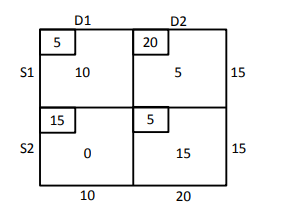
\includegraphics[width=0.75\columnwidth]{chapters/10/7/2/4/figs/fig.png}
 \end{center}
\caption{}
\label{fig:10/7/2/4Fig1}
\end{figure}
\fi

\item Find the position vector of the mid point of the vector joining the points $\vec{P}$(2, 3, 4)
and $\vec{Q}$(4, 1, –2).
\\
\solution
		\begin{enumerate}[label=\thesubsection.\arabic*,ref=\thesubsection.\theenumi]
\item Find the coordinates of the point which divides the join of $(-1,7) $ and $ (4,-3)$ in the ratio 2:3.
	\\
		\solution
	\input{chapters/10/7/2/1/section.tex}
\item Find the coordinates of the point $\vec{R}$ on the line segment joining the points $\vec{P}(-1,3)$ and $\vec{Q}(2,5)$ such that $PR=\frac{3}{5}PQ$.
\item Find the ratio in which the point $\vec{P}\brak{\frac{3}{4},\frac{5}{12}}$ divides the line segment joining the points $\vec{A}\brak{\frac{1}{2},\frac{3}{2}}$ and $ \vec{B}(2,-5)$.
\item Find the coordinates of the point which divides the line segment joining the points $(4,-3)$ and $(8,5)$ in the ratio $3:1$ internally.
\item Find the coordinates of the point $\vec{P}$ on $AD$ such that $AP : PD = 2 : 1$.
\item If the point $\vec{P} (2, 1)$ lies on the line segment joining points $\vec{A} (4, 2)$  and $ \vec{B} (8, 4)$,
then
\begin{enumerate}
	\item $AP =\frac{1}{3}{AB}$ 
\item ${AP}={PE}$
\item ${PB}=\frac{1}{3}{AB}$
\item${AP}=\frac{1}{2}{AB}$
 \end{enumerate}
\item Find the ratio in which the line segment joining the points $(-3,10)$  and  $(6,-8)$  is divided by $ (-1,6)$.
	\\
		\solution
	\input{chapters/10/7/2/4/section.tex}
\item Find the position vector of the mid point of the vector joining the points $\vec{P}$(2, 3, 4)
and $\vec{Q}$(4, 1, –2).
\\
\solution
		\input{chapters/12/10/2/16/section.tex}
\item Let $\vec{A}(4, 2), \vec{B}(6, 5)$  and $ \vec{C}(1, 4)$ be the vertices of $\triangle ABC$.
\begin{enumerate}
\item If $\vec{A}$ and  $\vec{B}$ are $(-2,-2)$ and  $(2,-4)$, respectively, find the coordinates of $\vec{P}$ such that $AP= \frac {3}{7}AB$  and $ \vec{P}$ lies on the line segment $AB$.
	\\
		\solution
	\input{chapters/10/7/2/8/section.tex}
\item Find the coordinates of the points which divide the line segment joining $A(-2,2)$  and  $\vec{B}(2,8)$ into four equal parts.
	\\
		\solution
	\input{chapters/10/7/2/9/section.tex}
\item In what ratio does the point $(-4,6)$ divide the line segment joining the points $\vec{A}(-6,0)$ and $\vec{B}(3,-8)$?
\item Given that $\vec{P}(3,2,-4), \vec{Q}(5,4,-6)$ and $\vec{R}(9,8,-10)$ are collinear. Find the ratio in which $\vec{Q}$ divides $PR$.
\item Points $\vec{A}(-6,10),\vec{B}(-4,6)$  and  $\vec{C}(3,-8)$ are collinear such that $AB=  \frac{2}{9}AC$.
\item The point which divides the line segment joining the points $\vec{P} (7, –6) $  and  $\vec{Q}(3, 4)$ in the 
ratio 1 : 2 internally lies in  which quadrant?
\item Find the coordinates of the points of trisection of the line segment joining $(4,-1)$  and  $(-2,3)$.
	\\
		\solution
	\input{chapters/10/7/2/2/section.tex}
\item Find the coordinates of the points which trisect the line segment joining the points $\vec{P}(4,2,-6)$ and $\vec{Q}(10,-16,6)$.
\item Find the coordinates of the points of trisection (i.e. points dividing to three equal parts) of the line segment joining the points $\vec{A}(2,-2)$ and $\vec{B}(-7,4)$.
\item Point $\vec{P}(5,-3)$ is one of the two points of trisection of line segment joining the points $\vec{A}(7,-2)$ and $\vec{B}(1,-5)$
\item Find the position vector of a point $\vec{R}$ which divides the line joining two points $\vec{P}$
and $\vec{Q}$ whose position vectors are $\hat{i}+2\hat{j}-\hat{k}$ and $-\hat{i}+\hat{j}+\hat{k}$ respectively, in the
ratio 2 : 1
\begin{enumerate}
    \item  internally
    \item  externally
\end{enumerate}
%\solution
%		\input{chapters/12/10/2/15/section.tex}
\item Find the coordinates of the point which divides the line segment joining the points which divides the line segment joining  the points $(-2,3,5)$ and $(1,-4,6)$ in the ratio 
\begin{enumerate}
\item $2:3$ internally,
\item $2:3$ externally
\end{enumerate}
\item Find the coordinates of the point which divides the line segment joining the points $(1,-2,3)$ and $(3,4,-5)$ in the ratio $2:3$
\begin{enumerate}
\item internally, and
\item externally
\end{enumerate}
\item Consider two points $\vec{P}$ and $\vec{Q}$ with position vectors $\overrightarrow{OP} = 3\overrightarrow{a}-2\overrightarrow{b}$ and $\overrightarrow{OQ}=\overrightarrow{a}+\overrightarrow{b}$. Find the position vector of a point $\vec{R}$ which divides the line joining $\vec{P}$ and $\vec{Q}$ in the ratio $2:1$, 
\begin{enumerate}
\item internally, and 
\item externally.
\end{enumerate}
\item The median from $\vec{A}$ meets $BC$ at $\vec{D}$. Find the coordinates of the point $\vec{D}$.
\item Find the coordinates of points $\vec{Q}$ and $\vec{R}$ on medians $BE$ and $CF$ respectively such that $BQ : QE = 2 : 1$  and  $CR : RF = 2 : 1$.
\item What do you observe?
\item If $\vec{A}, \vec{B}$ and $\vec{C}$  are the vertices of $\triangle ABC$, find the coordinates of the centroid of the triangle.
\end{enumerate}
\solution
	\input{chapters/10/7/4/7/section.tex}
\item If $\vec{P}(9a-2,-b)$ divides line segment joining $\vec{A}(3a+1,-3)$ and $\vec{B}(8a,5)$ in the ratio 3:1, find the values of $a$ and $b$.
\item Find the position vector of a point $\vec{R}$ which divides the line joining two points $\vec{P}$ and $\vec{Q}$ whose position vectors are $2\vec{a}+\vec{b}$ and $\vec{a}-3\vec{b}$ externally in the ratio $1:2$.
\item The position vector of the point which divides the join of points 2$\vec{a}$-3$\vec{b}$ $\text{and}$ $\vec{a}+\vec{b}$ in the ratio 3:1 is \rule{1cm}{0.1pt}.
\item If $\vec{a}$ and $\vec{b}$ are the postion vectors of $\vec{A}$ and $\vec{B}$, respectively, find the position vector of a point $\vec{C}$ in $BA$ produced such that $BC=1.5BA$.
\item Find the position vector of a point $\vec{R}$ which divides the line joining two points $\vec{P}$ and $\vec{Q}$ whose position vectors are $(2\vec{a}+\vec{b})$ and $(\vec{a}-3\vec{b})$
externally in the ratio 1 : 2. Also, show that $\vec{P}$ is the mid point of the line segment $RQ$.
\end{enumerate}

\item Let $\vec{A}(4, 2), \vec{B}(6, 5)$  and $ \vec{C}(1, 4)$ be the vertices of $\triangle ABC$.
\begin{enumerate}
\item If $\vec{A}$ and  $\vec{B}$ are $(-2,-2)$ and  $(2,-4)$, respectively, find the coordinates of $\vec{P}$ such that $AP= \frac {3}{7}AB$  and $ \vec{P}$ lies on the line segment $AB$.
	\\
		\solution
	\begin{enumerate}[label=\thesubsection.\arabic*,ref=\thesubsection.\theenumi]
\item Find the coordinates of the point which divides the join of $(-1,7) $ and $ (4,-3)$ in the ratio 2:3.
	\\
		\solution
	\input{chapters/10/7/2/1/section.tex}
\item Find the coordinates of the point $\vec{R}$ on the line segment joining the points $\vec{P}(-1,3)$ and $\vec{Q}(2,5)$ such that $PR=\frac{3}{5}PQ$.
\item Find the ratio in which the point $\vec{P}\brak{\frac{3}{4},\frac{5}{12}}$ divides the line segment joining the points $\vec{A}\brak{\frac{1}{2},\frac{3}{2}}$ and $ \vec{B}(2,-5)$.
\item Find the coordinates of the point which divides the line segment joining the points $(4,-3)$ and $(8,5)$ in the ratio $3:1$ internally.
\item Find the coordinates of the point $\vec{P}$ on $AD$ such that $AP : PD = 2 : 1$.
\item If the point $\vec{P} (2, 1)$ lies on the line segment joining points $\vec{A} (4, 2)$  and $ \vec{B} (8, 4)$,
then
\begin{enumerate}
	\item $AP =\frac{1}{3}{AB}$ 
\item ${AP}={PE}$
\item ${PB}=\frac{1}{3}{AB}$
\item${AP}=\frac{1}{2}{AB}$
 \end{enumerate}
\item Find the ratio in which the line segment joining the points $(-3,10)$  and  $(6,-8)$  is divided by $ (-1,6)$.
	\\
		\solution
	\input{chapters/10/7/2/4/section.tex}
\item Find the position vector of the mid point of the vector joining the points $\vec{P}$(2, 3, 4)
and $\vec{Q}$(4, 1, –2).
\\
\solution
		\input{chapters/12/10/2/16/section.tex}
\item Let $\vec{A}(4, 2), \vec{B}(6, 5)$  and $ \vec{C}(1, 4)$ be the vertices of $\triangle ABC$.
\begin{enumerate}
\item If $\vec{A}$ and  $\vec{B}$ are $(-2,-2)$ and  $(2,-4)$, respectively, find the coordinates of $\vec{P}$ such that $AP= \frac {3}{7}AB$  and $ \vec{P}$ lies on the line segment $AB$.
	\\
		\solution
	\input{chapters/10/7/2/8/section.tex}
\item Find the coordinates of the points which divide the line segment joining $A(-2,2)$  and  $\vec{B}(2,8)$ into four equal parts.
	\\
		\solution
	\input{chapters/10/7/2/9/section.tex}
\item In what ratio does the point $(-4,6)$ divide the line segment joining the points $\vec{A}(-6,0)$ and $\vec{B}(3,-8)$?
\item Given that $\vec{P}(3,2,-4), \vec{Q}(5,4,-6)$ and $\vec{R}(9,8,-10)$ are collinear. Find the ratio in which $\vec{Q}$ divides $PR$.
\item Points $\vec{A}(-6,10),\vec{B}(-4,6)$  and  $\vec{C}(3,-8)$ are collinear such that $AB=  \frac{2}{9}AC$.
\item The point which divides the line segment joining the points $\vec{P} (7, –6) $  and  $\vec{Q}(3, 4)$ in the 
ratio 1 : 2 internally lies in  which quadrant?
\item Find the coordinates of the points of trisection of the line segment joining $(4,-1)$  and  $(-2,3)$.
	\\
		\solution
	\input{chapters/10/7/2/2/section.tex}
\item Find the coordinates of the points which trisect the line segment joining the points $\vec{P}(4,2,-6)$ and $\vec{Q}(10,-16,6)$.
\item Find the coordinates of the points of trisection (i.e. points dividing to three equal parts) of the line segment joining the points $\vec{A}(2,-2)$ and $\vec{B}(-7,4)$.
\item Point $\vec{P}(5,-3)$ is one of the two points of trisection of line segment joining the points $\vec{A}(7,-2)$ and $\vec{B}(1,-5)$
\item Find the position vector of a point $\vec{R}$ which divides the line joining two points $\vec{P}$
and $\vec{Q}$ whose position vectors are $\hat{i}+2\hat{j}-\hat{k}$ and $-\hat{i}+\hat{j}+\hat{k}$ respectively, in the
ratio 2 : 1
\begin{enumerate}
    \item  internally
    \item  externally
\end{enumerate}
%\solution
%		\input{chapters/12/10/2/15/section.tex}
\item Find the coordinates of the point which divides the line segment joining the points which divides the line segment joining  the points $(-2,3,5)$ and $(1,-4,6)$ in the ratio 
\begin{enumerate}
\item $2:3$ internally,
\item $2:3$ externally
\end{enumerate}
\item Find the coordinates of the point which divides the line segment joining the points $(1,-2,3)$ and $(3,4,-5)$ in the ratio $2:3$
\begin{enumerate}
\item internally, and
\item externally
\end{enumerate}
\item Consider two points $\vec{P}$ and $\vec{Q}$ with position vectors $\overrightarrow{OP} = 3\overrightarrow{a}-2\overrightarrow{b}$ and $\overrightarrow{OQ}=\overrightarrow{a}+\overrightarrow{b}$. Find the position vector of a point $\vec{R}$ which divides the line joining $\vec{P}$ and $\vec{Q}$ in the ratio $2:1$, 
\begin{enumerate}
\item internally, and 
\item externally.
\end{enumerate}
\item The median from $\vec{A}$ meets $BC$ at $\vec{D}$. Find the coordinates of the point $\vec{D}$.
\item Find the coordinates of points $\vec{Q}$ and $\vec{R}$ on medians $BE$ and $CF$ respectively such that $BQ : QE = 2 : 1$  and  $CR : RF = 2 : 1$.
\item What do you observe?
\item If $\vec{A}, \vec{B}$ and $\vec{C}$  are the vertices of $\triangle ABC$, find the coordinates of the centroid of the triangle.
\end{enumerate}
\solution
	\input{chapters/10/7/4/7/section.tex}
\item If $\vec{P}(9a-2,-b)$ divides line segment joining $\vec{A}(3a+1,-3)$ and $\vec{B}(8a,5)$ in the ratio 3:1, find the values of $a$ and $b$.
\item Find the position vector of a point $\vec{R}$ which divides the line joining two points $\vec{P}$ and $\vec{Q}$ whose position vectors are $2\vec{a}+\vec{b}$ and $\vec{a}-3\vec{b}$ externally in the ratio $1:2$.
\item The position vector of the point which divides the join of points 2$\vec{a}$-3$\vec{b}$ $\text{and}$ $\vec{a}+\vec{b}$ in the ratio 3:1 is \rule{1cm}{0.1pt}.
\item If $\vec{a}$ and $\vec{b}$ are the postion vectors of $\vec{A}$ and $\vec{B}$, respectively, find the position vector of a point $\vec{C}$ in $BA$ produced such that $BC=1.5BA$.
\item Find the position vector of a point $\vec{R}$ which divides the line joining two points $\vec{P}$ and $\vec{Q}$ whose position vectors are $(2\vec{a}+\vec{b})$ and $(\vec{a}-3\vec{b})$
externally in the ratio 1 : 2. Also, show that $\vec{P}$ is the mid point of the line segment $RQ$.
\end{enumerate}

\item Find the coordinates of the points which divide the line segment joining $A(-2,2)$  and  $\vec{B}(2,8)$ into four equal parts.
	\\
		\solution
	\begin{enumerate}[label=\thesubsection.\arabic*,ref=\thesubsection.\theenumi]
\item Find the coordinates of the point which divides the join of $(-1,7) $ and $ (4,-3)$ in the ratio 2:3.
	\\
		\solution
	\input{chapters/10/7/2/1/section.tex}
\item Find the coordinates of the point $\vec{R}$ on the line segment joining the points $\vec{P}(-1,3)$ and $\vec{Q}(2,5)$ such that $PR=\frac{3}{5}PQ$.
\item Find the ratio in which the point $\vec{P}\brak{\frac{3}{4},\frac{5}{12}}$ divides the line segment joining the points $\vec{A}\brak{\frac{1}{2},\frac{3}{2}}$ and $ \vec{B}(2,-5)$.
\item Find the coordinates of the point which divides the line segment joining the points $(4,-3)$ and $(8,5)$ in the ratio $3:1$ internally.
\item Find the coordinates of the point $\vec{P}$ on $AD$ such that $AP : PD = 2 : 1$.
\item If the point $\vec{P} (2, 1)$ lies on the line segment joining points $\vec{A} (4, 2)$  and $ \vec{B} (8, 4)$,
then
\begin{enumerate}
	\item $AP =\frac{1}{3}{AB}$ 
\item ${AP}={PE}$
\item ${PB}=\frac{1}{3}{AB}$
\item${AP}=\frac{1}{2}{AB}$
 \end{enumerate}
\item Find the ratio in which the line segment joining the points $(-3,10)$  and  $(6,-8)$  is divided by $ (-1,6)$.
	\\
		\solution
	\input{chapters/10/7/2/4/section.tex}
\item Find the position vector of the mid point of the vector joining the points $\vec{P}$(2, 3, 4)
and $\vec{Q}$(4, 1, –2).
\\
\solution
		\input{chapters/12/10/2/16/section.tex}
\item Let $\vec{A}(4, 2), \vec{B}(6, 5)$  and $ \vec{C}(1, 4)$ be the vertices of $\triangle ABC$.
\begin{enumerate}
\item If $\vec{A}$ and  $\vec{B}$ are $(-2,-2)$ and  $(2,-4)$, respectively, find the coordinates of $\vec{P}$ such that $AP= \frac {3}{7}AB$  and $ \vec{P}$ lies on the line segment $AB$.
	\\
		\solution
	\input{chapters/10/7/2/8/section.tex}
\item Find the coordinates of the points which divide the line segment joining $A(-2,2)$  and  $\vec{B}(2,8)$ into four equal parts.
	\\
		\solution
	\input{chapters/10/7/2/9/section.tex}
\item In what ratio does the point $(-4,6)$ divide the line segment joining the points $\vec{A}(-6,0)$ and $\vec{B}(3,-8)$?
\item Given that $\vec{P}(3,2,-4), \vec{Q}(5,4,-6)$ and $\vec{R}(9,8,-10)$ are collinear. Find the ratio in which $\vec{Q}$ divides $PR$.
\item Points $\vec{A}(-6,10),\vec{B}(-4,6)$  and  $\vec{C}(3,-8)$ are collinear such that $AB=  \frac{2}{9}AC$.
\item The point which divides the line segment joining the points $\vec{P} (7, –6) $  and  $\vec{Q}(3, 4)$ in the 
ratio 1 : 2 internally lies in  which quadrant?
\item Find the coordinates of the points of trisection of the line segment joining $(4,-1)$  and  $(-2,3)$.
	\\
		\solution
	\input{chapters/10/7/2/2/section.tex}
\item Find the coordinates of the points which trisect the line segment joining the points $\vec{P}(4,2,-6)$ and $\vec{Q}(10,-16,6)$.
\item Find the coordinates of the points of trisection (i.e. points dividing to three equal parts) of the line segment joining the points $\vec{A}(2,-2)$ and $\vec{B}(-7,4)$.
\item Point $\vec{P}(5,-3)$ is one of the two points of trisection of line segment joining the points $\vec{A}(7,-2)$ and $\vec{B}(1,-5)$
\item Find the position vector of a point $\vec{R}$ which divides the line joining two points $\vec{P}$
and $\vec{Q}$ whose position vectors are $\hat{i}+2\hat{j}-\hat{k}$ and $-\hat{i}+\hat{j}+\hat{k}$ respectively, in the
ratio 2 : 1
\begin{enumerate}
    \item  internally
    \item  externally
\end{enumerate}
%\solution
%		\input{chapters/12/10/2/15/section.tex}
\item Find the coordinates of the point which divides the line segment joining the points which divides the line segment joining  the points $(-2,3,5)$ and $(1,-4,6)$ in the ratio 
\begin{enumerate}
\item $2:3$ internally,
\item $2:3$ externally
\end{enumerate}
\item Find the coordinates of the point which divides the line segment joining the points $(1,-2,3)$ and $(3,4,-5)$ in the ratio $2:3$
\begin{enumerate}
\item internally, and
\item externally
\end{enumerate}
\item Consider two points $\vec{P}$ and $\vec{Q}$ with position vectors $\overrightarrow{OP} = 3\overrightarrow{a}-2\overrightarrow{b}$ and $\overrightarrow{OQ}=\overrightarrow{a}+\overrightarrow{b}$. Find the position vector of a point $\vec{R}$ which divides the line joining $\vec{P}$ and $\vec{Q}$ in the ratio $2:1$, 
\begin{enumerate}
\item internally, and 
\item externally.
\end{enumerate}
\item The median from $\vec{A}$ meets $BC$ at $\vec{D}$. Find the coordinates of the point $\vec{D}$.
\item Find the coordinates of points $\vec{Q}$ and $\vec{R}$ on medians $BE$ and $CF$ respectively such that $BQ : QE = 2 : 1$  and  $CR : RF = 2 : 1$.
\item What do you observe?
\item If $\vec{A}, \vec{B}$ and $\vec{C}$  are the vertices of $\triangle ABC$, find the coordinates of the centroid of the triangle.
\end{enumerate}
\solution
	\input{chapters/10/7/4/7/section.tex}
\item If $\vec{P}(9a-2,-b)$ divides line segment joining $\vec{A}(3a+1,-3)$ and $\vec{B}(8a,5)$ in the ratio 3:1, find the values of $a$ and $b$.
\item Find the position vector of a point $\vec{R}$ which divides the line joining two points $\vec{P}$ and $\vec{Q}$ whose position vectors are $2\vec{a}+\vec{b}$ and $\vec{a}-3\vec{b}$ externally in the ratio $1:2$.
\item The position vector of the point which divides the join of points 2$\vec{a}$-3$\vec{b}$ $\text{and}$ $\vec{a}+\vec{b}$ in the ratio 3:1 is \rule{1cm}{0.1pt}.
\item If $\vec{a}$ and $\vec{b}$ are the postion vectors of $\vec{A}$ and $\vec{B}$, respectively, find the position vector of a point $\vec{C}$ in $BA$ produced such that $BC=1.5BA$.
\item Find the position vector of a point $\vec{R}$ which divides the line joining two points $\vec{P}$ and $\vec{Q}$ whose position vectors are $(2\vec{a}+\vec{b})$ and $(\vec{a}-3\vec{b})$
externally in the ratio 1 : 2. Also, show that $\vec{P}$ is the mid point of the line segment $RQ$.
\end{enumerate}

\item In what ratio does the point $(-4,6)$ divide the line segment joining the points $\vec{A}(-6,0)$ and $\vec{B}(3,-8)$?
\item Given that $\vec{P}(3,2,-4), \vec{Q}(5,4,-6)$ and $\vec{R}(9,8,-10)$ are collinear. Find the ratio in which $\vec{Q}$ divides $PR$.
\item Points $\vec{A}(-6,10),\vec{B}(-4,6)$  and  $\vec{C}(3,-8)$ are collinear such that $AB=  \frac{2}{9}AC$.
\item The point which divides the line segment joining the points $\vec{P} (7, –6) $  and  $\vec{Q}(3, 4)$ in the 
ratio 1 : 2 internally lies in  which quadrant?
\item Find the coordinates of the points of trisection of the line segment joining $(4,-1)$  and  $(-2,3)$.
	\\
		\solution
	Using section formula,
\begin{align}
\vec{R}=\frac{1}{1+\frac{1}{2}}\brak{\myvec{4\\-1}+\frac{1}{2}\myvec{-2\\3}}
=\myvec{2\\ \frac{1}{3}}\\
\vec{S}=\frac{1}{1+\frac{2}{1}}\brak{\myvec{4\\-1}+\frac{2}{1}\myvec{-2\\3}}
=\myvec{0\\ \frac{5}{3}}
\end{align}
which are the desired points of trisection.
\iffalse
See
		\figref{fig:chapters/10/7/2/2/Figure}
\begin{figure}[H]
\centering
\includegraphics[width=0.75\columnwidth]{chapters/10/7/2/2/figs/dj.pdf}
\caption{}
		\label{fig:chapters/10/7/2/2/Figure}
\end{figure}
\fi

\item Find the coordinates of the points which trisect the line segment joining the points $\vec{P}(4,2,-6)$ and $\vec{Q}(10,-16,6)$.
\item Find the coordinates of the points of trisection (i.e. points dividing to three equal parts) of the line segment joining the points $\vec{A}(2,-2)$ and $\vec{B}(-7,4)$.
\item Point $\vec{P}(5,-3)$ is one of the two points of trisection of line segment joining the points $\vec{A}(7,-2)$ and $\vec{B}(1,-5)$
\item Find the position vector of a point $\vec{R}$ which divides the line joining two points $\vec{P}$
and $\vec{Q}$ whose position vectors are $\hat{i}+2\hat{j}-\hat{k}$ and $-\hat{i}+\hat{j}+\hat{k}$ respectively, in the
ratio 2 : 1
\begin{enumerate}
    \item  internally
    \item  externally
\end{enumerate}
%\solution
%		\begin{enumerate}[label=\thesubsection.\arabic*,ref=\thesubsection.\theenumi]
\item Find the coordinates of the point which divides the join of $(-1,7) $ and $ (4,-3)$ in the ratio 2:3.
	\\
		\solution
	\input{chapters/10/7/2/1/section.tex}
\item Find the coordinates of the point $\vec{R}$ on the line segment joining the points $\vec{P}(-1,3)$ and $\vec{Q}(2,5)$ such that $PR=\frac{3}{5}PQ$.
\item Find the ratio in which the point $\vec{P}\brak{\frac{3}{4},\frac{5}{12}}$ divides the line segment joining the points $\vec{A}\brak{\frac{1}{2},\frac{3}{2}}$ and $ \vec{B}(2,-5)$.
\item Find the coordinates of the point which divides the line segment joining the points $(4,-3)$ and $(8,5)$ in the ratio $3:1$ internally.
\item Find the coordinates of the point $\vec{P}$ on $AD$ such that $AP : PD = 2 : 1$.
\item If the point $\vec{P} (2, 1)$ lies on the line segment joining points $\vec{A} (4, 2)$  and $ \vec{B} (8, 4)$,
then
\begin{enumerate}
	\item $AP =\frac{1}{3}{AB}$ 
\item ${AP}={PE}$
\item ${PB}=\frac{1}{3}{AB}$
\item${AP}=\frac{1}{2}{AB}$
 \end{enumerate}
\item Find the ratio in which the line segment joining the points $(-3,10)$  and  $(6,-8)$  is divided by $ (-1,6)$.
	\\
		\solution
	\input{chapters/10/7/2/4/section.tex}
\item Find the position vector of the mid point of the vector joining the points $\vec{P}$(2, 3, 4)
and $\vec{Q}$(4, 1, –2).
\\
\solution
		\input{chapters/12/10/2/16/section.tex}
\item Let $\vec{A}(4, 2), \vec{B}(6, 5)$  and $ \vec{C}(1, 4)$ be the vertices of $\triangle ABC$.
\begin{enumerate}
\item If $\vec{A}$ and  $\vec{B}$ are $(-2,-2)$ and  $(2,-4)$, respectively, find the coordinates of $\vec{P}$ such that $AP= \frac {3}{7}AB$  and $ \vec{P}$ lies on the line segment $AB$.
	\\
		\solution
	\input{chapters/10/7/2/8/section.tex}
\item Find the coordinates of the points which divide the line segment joining $A(-2,2)$  and  $\vec{B}(2,8)$ into four equal parts.
	\\
		\solution
	\input{chapters/10/7/2/9/section.tex}
\item In what ratio does the point $(-4,6)$ divide the line segment joining the points $\vec{A}(-6,0)$ and $\vec{B}(3,-8)$?
\item Given that $\vec{P}(3,2,-4), \vec{Q}(5,4,-6)$ and $\vec{R}(9,8,-10)$ are collinear. Find the ratio in which $\vec{Q}$ divides $PR$.
\item Points $\vec{A}(-6,10),\vec{B}(-4,6)$  and  $\vec{C}(3,-8)$ are collinear such that $AB=  \frac{2}{9}AC$.
\item The point which divides the line segment joining the points $\vec{P} (7, –6) $  and  $\vec{Q}(3, 4)$ in the 
ratio 1 : 2 internally lies in  which quadrant?
\item Find the coordinates of the points of trisection of the line segment joining $(4,-1)$  and  $(-2,3)$.
	\\
		\solution
	\input{chapters/10/7/2/2/section.tex}
\item Find the coordinates of the points which trisect the line segment joining the points $\vec{P}(4,2,-6)$ and $\vec{Q}(10,-16,6)$.
\item Find the coordinates of the points of trisection (i.e. points dividing to three equal parts) of the line segment joining the points $\vec{A}(2,-2)$ and $\vec{B}(-7,4)$.
\item Point $\vec{P}(5,-3)$ is one of the two points of trisection of line segment joining the points $\vec{A}(7,-2)$ and $\vec{B}(1,-5)$
\item Find the position vector of a point $\vec{R}$ which divides the line joining two points $\vec{P}$
and $\vec{Q}$ whose position vectors are $\hat{i}+2\hat{j}-\hat{k}$ and $-\hat{i}+\hat{j}+\hat{k}$ respectively, in the
ratio 2 : 1
\begin{enumerate}
    \item  internally
    \item  externally
\end{enumerate}
%\solution
%		\input{chapters/12/10/2/15/section.tex}
\item Find the coordinates of the point which divides the line segment joining the points which divides the line segment joining  the points $(-2,3,5)$ and $(1,-4,6)$ in the ratio 
\begin{enumerate}
\item $2:3$ internally,
\item $2:3$ externally
\end{enumerate}
\item Find the coordinates of the point which divides the line segment joining the points $(1,-2,3)$ and $(3,4,-5)$ in the ratio $2:3$
\begin{enumerate}
\item internally, and
\item externally
\end{enumerate}
\item Consider two points $\vec{P}$ and $\vec{Q}$ with position vectors $\overrightarrow{OP} = 3\overrightarrow{a}-2\overrightarrow{b}$ and $\overrightarrow{OQ}=\overrightarrow{a}+\overrightarrow{b}$. Find the position vector of a point $\vec{R}$ which divides the line joining $\vec{P}$ and $\vec{Q}$ in the ratio $2:1$, 
\begin{enumerate}
\item internally, and 
\item externally.
\end{enumerate}
\item The median from $\vec{A}$ meets $BC$ at $\vec{D}$. Find the coordinates of the point $\vec{D}$.
\item Find the coordinates of points $\vec{Q}$ and $\vec{R}$ on medians $BE$ and $CF$ respectively such that $BQ : QE = 2 : 1$  and  $CR : RF = 2 : 1$.
\item What do you observe?
\item If $\vec{A}, \vec{B}$ and $\vec{C}$  are the vertices of $\triangle ABC$, find the coordinates of the centroid of the triangle.
\end{enumerate}
\solution
	\input{chapters/10/7/4/7/section.tex}
\item If $\vec{P}(9a-2,-b)$ divides line segment joining $\vec{A}(3a+1,-3)$ and $\vec{B}(8a,5)$ in the ratio 3:1, find the values of $a$ and $b$.
\item Find the position vector of a point $\vec{R}$ which divides the line joining two points $\vec{P}$ and $\vec{Q}$ whose position vectors are $2\vec{a}+\vec{b}$ and $\vec{a}-3\vec{b}$ externally in the ratio $1:2$.
\item The position vector of the point which divides the join of points 2$\vec{a}$-3$\vec{b}$ $\text{and}$ $\vec{a}+\vec{b}$ in the ratio 3:1 is \rule{1cm}{0.1pt}.
\item If $\vec{a}$ and $\vec{b}$ are the postion vectors of $\vec{A}$ and $\vec{B}$, respectively, find the position vector of a point $\vec{C}$ in $BA$ produced such that $BC=1.5BA$.
\item Find the position vector of a point $\vec{R}$ which divides the line joining two points $\vec{P}$ and $\vec{Q}$ whose position vectors are $(2\vec{a}+\vec{b})$ and $(\vec{a}-3\vec{b})$
externally in the ratio 1 : 2. Also, show that $\vec{P}$ is the mid point of the line segment $RQ$.
\end{enumerate}

\item Find the coordinates of the point which divides the line segment joining the points which divides the line segment joining  the points $(-2,3,5)$ and $(1,-4,6)$ in the ratio 
\begin{enumerate}
\item $2:3$ internally,
\item $2:3$ externally
\end{enumerate}
\item Find the coordinates of the point which divides the line segment joining the points $(1,-2,3)$ and $(3,4,-5)$ in the ratio $2:3$
\begin{enumerate}
\item internally, and
\item externally
\end{enumerate}
\item Consider two points $\vec{P}$ and $\vec{Q}$ with position vectors $\overrightarrow{OP} = 3\overrightarrow{a}-2\overrightarrow{b}$ and $\overrightarrow{OQ}=\overrightarrow{a}+\overrightarrow{b}$. Find the position vector of a point $\vec{R}$ which divides the line joining $\vec{P}$ and $\vec{Q}$ in the ratio $2:1$, 
\begin{enumerate}
\item internally, and 
\item externally.
\end{enumerate}
\item The median from $\vec{A}$ meets $BC$ at $\vec{D}$. Find the coordinates of the point $\vec{D}$.
\item Find the coordinates of points $\vec{Q}$ and $\vec{R}$ on medians $BE$ and $CF$ respectively such that $BQ : QE = 2 : 1$  and  $CR : RF = 2 : 1$.
\item What do you observe?
\item If $\vec{A}, \vec{B}$ and $\vec{C}$  are the vertices of $\triangle ABC$, find the coordinates of the centroid of the triangle.
\end{enumerate}
\solution
	\begin{enumerate}[label=\thesubsection.\arabic*,ref=\thesubsection.\theenumi]
\item Find the coordinates of the point which divides the join of $(-1,7) $ and $ (4,-3)$ in the ratio 2:3.
	\\
		\solution
	\input{chapters/10/7/2/1/section.tex}
\item Find the coordinates of the point $\vec{R}$ on the line segment joining the points $\vec{P}(-1,3)$ and $\vec{Q}(2,5)$ such that $PR=\frac{3}{5}PQ$.
\item Find the ratio in which the point $\vec{P}\brak{\frac{3}{4},\frac{5}{12}}$ divides the line segment joining the points $\vec{A}\brak{\frac{1}{2},\frac{3}{2}}$ and $ \vec{B}(2,-5)$.
\item Find the coordinates of the point which divides the line segment joining the points $(4,-3)$ and $(8,5)$ in the ratio $3:1$ internally.
\item Find the coordinates of the point $\vec{P}$ on $AD$ such that $AP : PD = 2 : 1$.
\item If the point $\vec{P} (2, 1)$ lies on the line segment joining points $\vec{A} (4, 2)$  and $ \vec{B} (8, 4)$,
then
\begin{enumerate}
	\item $AP =\frac{1}{3}{AB}$ 
\item ${AP}={PE}$
\item ${PB}=\frac{1}{3}{AB}$
\item${AP}=\frac{1}{2}{AB}$
 \end{enumerate}
\item Find the ratio in which the line segment joining the points $(-3,10)$  and  $(6,-8)$  is divided by $ (-1,6)$.
	\\
		\solution
	\input{chapters/10/7/2/4/section.tex}
\item Find the position vector of the mid point of the vector joining the points $\vec{P}$(2, 3, 4)
and $\vec{Q}$(4, 1, –2).
\\
\solution
		\input{chapters/12/10/2/16/section.tex}
\item Let $\vec{A}(4, 2), \vec{B}(6, 5)$  and $ \vec{C}(1, 4)$ be the vertices of $\triangle ABC$.
\begin{enumerate}
\item If $\vec{A}$ and  $\vec{B}$ are $(-2,-2)$ and  $(2,-4)$, respectively, find the coordinates of $\vec{P}$ such that $AP= \frac {3}{7}AB$  and $ \vec{P}$ lies on the line segment $AB$.
	\\
		\solution
	\input{chapters/10/7/2/8/section.tex}
\item Find the coordinates of the points which divide the line segment joining $A(-2,2)$  and  $\vec{B}(2,8)$ into four equal parts.
	\\
		\solution
	\input{chapters/10/7/2/9/section.tex}
\item In what ratio does the point $(-4,6)$ divide the line segment joining the points $\vec{A}(-6,0)$ and $\vec{B}(3,-8)$?
\item Given that $\vec{P}(3,2,-4), \vec{Q}(5,4,-6)$ and $\vec{R}(9,8,-10)$ are collinear. Find the ratio in which $\vec{Q}$ divides $PR$.
\item Points $\vec{A}(-6,10),\vec{B}(-4,6)$  and  $\vec{C}(3,-8)$ are collinear such that $AB=  \frac{2}{9}AC$.
\item The point which divides the line segment joining the points $\vec{P} (7, –6) $  and  $\vec{Q}(3, 4)$ in the 
ratio 1 : 2 internally lies in  which quadrant?
\item Find the coordinates of the points of trisection of the line segment joining $(4,-1)$  and  $(-2,3)$.
	\\
		\solution
	\input{chapters/10/7/2/2/section.tex}
\item Find the coordinates of the points which trisect the line segment joining the points $\vec{P}(4,2,-6)$ and $\vec{Q}(10,-16,6)$.
\item Find the coordinates of the points of trisection (i.e. points dividing to three equal parts) of the line segment joining the points $\vec{A}(2,-2)$ and $\vec{B}(-7,4)$.
\item Point $\vec{P}(5,-3)$ is one of the two points of trisection of line segment joining the points $\vec{A}(7,-2)$ and $\vec{B}(1,-5)$
\item Find the position vector of a point $\vec{R}$ which divides the line joining two points $\vec{P}$
and $\vec{Q}$ whose position vectors are $\hat{i}+2\hat{j}-\hat{k}$ and $-\hat{i}+\hat{j}+\hat{k}$ respectively, in the
ratio 2 : 1
\begin{enumerate}
    \item  internally
    \item  externally
\end{enumerate}
%\solution
%		\input{chapters/12/10/2/15/section.tex}
\item Find the coordinates of the point which divides the line segment joining the points which divides the line segment joining  the points $(-2,3,5)$ and $(1,-4,6)$ in the ratio 
\begin{enumerate}
\item $2:3$ internally,
\item $2:3$ externally
\end{enumerate}
\item Find the coordinates of the point which divides the line segment joining the points $(1,-2,3)$ and $(3,4,-5)$ in the ratio $2:3$
\begin{enumerate}
\item internally, and
\item externally
\end{enumerate}
\item Consider two points $\vec{P}$ and $\vec{Q}$ with position vectors $\overrightarrow{OP} = 3\overrightarrow{a}-2\overrightarrow{b}$ and $\overrightarrow{OQ}=\overrightarrow{a}+\overrightarrow{b}$. Find the position vector of a point $\vec{R}$ which divides the line joining $\vec{P}$ and $\vec{Q}$ in the ratio $2:1$, 
\begin{enumerate}
\item internally, and 
\item externally.
\end{enumerate}
\item The median from $\vec{A}$ meets $BC$ at $\vec{D}$. Find the coordinates of the point $\vec{D}$.
\item Find the coordinates of points $\vec{Q}$ and $\vec{R}$ on medians $BE$ and $CF$ respectively such that $BQ : QE = 2 : 1$  and  $CR : RF = 2 : 1$.
\item What do you observe?
\item If $\vec{A}, \vec{B}$ and $\vec{C}$  are the vertices of $\triangle ABC$, find the coordinates of the centroid of the triangle.
\end{enumerate}
\solution
	\input{chapters/10/7/4/7/section.tex}
\item If $\vec{P}(9a-2,-b)$ divides line segment joining $\vec{A}(3a+1,-3)$ and $\vec{B}(8a,5)$ in the ratio 3:1, find the values of $a$ and $b$.
\item Find the position vector of a point $\vec{R}$ which divides the line joining two points $\vec{P}$ and $\vec{Q}$ whose position vectors are $2\vec{a}+\vec{b}$ and $\vec{a}-3\vec{b}$ externally in the ratio $1:2$.
\item The position vector of the point which divides the join of points 2$\vec{a}$-3$\vec{b}$ $\text{and}$ $\vec{a}+\vec{b}$ in the ratio 3:1 is \rule{1cm}{0.1pt}.
\item If $\vec{a}$ and $\vec{b}$ are the postion vectors of $\vec{A}$ and $\vec{B}$, respectively, find the position vector of a point $\vec{C}$ in $BA$ produced such that $BC=1.5BA$.
\item Find the position vector of a point $\vec{R}$ which divides the line joining two points $\vec{P}$ and $\vec{Q}$ whose position vectors are $(2\vec{a}+\vec{b})$ and $(\vec{a}-3\vec{b})$
externally in the ratio 1 : 2. Also, show that $\vec{P}$ is the mid point of the line segment $RQ$.
\end{enumerate}

\item If $\vec{P}(9a-2,-b)$ divides line segment joining $\vec{A}(3a+1,-3)$ and $\vec{B}(8a,5)$ in the ratio 3:1, find the values of $a$ and $b$.
\item Find the position vector of a point $\vec{R}$ which divides the line joining two points $\vec{P}$ and $\vec{Q}$ whose position vectors are $2\vec{a}+\vec{b}$ and $\vec{a}-3\vec{b}$ externally in the ratio $1:2$.
\item The position vector of the point which divides the join of points 2$\vec{a}$-3$\vec{b}$ $\text{and}$ $\vec{a}+\vec{b}$ in the ratio 3:1 is \rule{1cm}{0.1pt}.
\item If $\vec{a}$ and $\vec{b}$ are the postion vectors of $\vec{A}$ and $\vec{B}$, respectively, find the position vector of a point $\vec{C}$ in $BA$ produced such that $BC=1.5BA$.
\item Find the position vector of a point $\vec{R}$ which divides the line joining two points $\vec{P}$ and $\vec{Q}$ whose position vectors are $(2\vec{a}+\vec{b})$ and $(\vec{a}-3\vec{b})$
externally in the ratio 1 : 2. Also, show that $\vec{P}$ is the mid point of the line segment $RQ$.
\end{enumerate}

\item In what ratio does the point $(-4,6)$ divide the line segment joining the points $\vec{A}(-6,0)$ and $\vec{B}(3,-8)$?
\item Given that $\vec{P}(3,2,-4), \vec{Q}(5,4,-6)$ and $\vec{R}(9,8,-10)$ are collinear. Find the ratio in which $\vec{Q}$ divides $PR$.
\item Points $\vec{A}(-6,10),\vec{B}(-4,6)$  and  $\vec{C}(3,-8)$ are collinear such that $AB=  \frac{2}{9}AC$.
\item The point which divides the line segment joining the points $\vec{P} (7, –6) $  and  $\vec{Q}(3, 4)$ in the 
ratio 1 : 2 internally lies in  which quadrant?
\item Find the coordinates of the points of trisection of the line segment joining $(4,-1)$  and  $(-2,3)$.
	\\
		\solution
	Using section formula,
\begin{align}
\vec{R}=\frac{1}{1+\frac{1}{2}}\brak{\myvec{4\\-1}+\frac{1}{2}\myvec{-2\\3}}
=\myvec{2\\ \frac{1}{3}}\\
\vec{S}=\frac{1}{1+\frac{2}{1}}\brak{\myvec{4\\-1}+\frac{2}{1}\myvec{-2\\3}}
=\myvec{0\\ \frac{5}{3}}
\end{align}
which are the desired points of trisection.
\iffalse
See
		\figref{fig:chapters/10/7/2/2/Figure}
\begin{figure}[H]
\centering
\includegraphics[width=0.75\columnwidth]{chapters/10/7/2/2/figs/dj.pdf}
\caption{}
		\label{fig:chapters/10/7/2/2/Figure}
\end{figure}
\fi

\item Find the coordinates of the points which trisect the line segment joining the points $\vec{P}(4,2,-6)$ and $\vec{Q}(10,-16,6)$.
\item Find the coordinates of the points of trisection (i.e. points dividing to three equal parts) of the line segment joining the points $\vec{A}(2,-2)$ and $\vec{B}(-7,4)$.
\item Point $\vec{P}(5,-3)$ is one of the two points of trisection of line segment joining the points $\vec{A}(7,-2)$ and $\vec{B}(1,-5)$
\item Find the position vector of a point $\vec{R}$ which divides the line joining two points $\vec{P}$
and $\vec{Q}$ whose position vectors are $\hat{i}+2\hat{j}-\hat{k}$ and $-\hat{i}+\hat{j}+\hat{k}$ respectively, in the
ratio 2 : 1
\begin{enumerate}
    \item  internally
    \item  externally
\end{enumerate}
%\solution
%		\begin{enumerate}[label=\thesubsection.\arabic*,ref=\thesubsection.\theenumi]
\item Find the coordinates of the point which divides the join of $(-1,7) $ and $ (4,-3)$ in the ratio 2:3.
	\\
		\solution
	\begin{enumerate}[label=\thesubsection.\arabic*,ref=\thesubsection.\theenumi]
\item Find the coordinates of the point which divides the join of $(-1,7) $ and $ (4,-3)$ in the ratio 2:3.
	\\
		\solution
	\input{chapters/10/7/2/1/section.tex}
\item Find the coordinates of the point $\vec{R}$ on the line segment joining the points $\vec{P}(-1,3)$ and $\vec{Q}(2,5)$ such that $PR=\frac{3}{5}PQ$.
\item Find the ratio in which the point $\vec{P}\brak{\frac{3}{4},\frac{5}{12}}$ divides the line segment joining the points $\vec{A}\brak{\frac{1}{2},\frac{3}{2}}$ and $ \vec{B}(2,-5)$.
\item Find the coordinates of the point which divides the line segment joining the points $(4,-3)$ and $(8,5)$ in the ratio $3:1$ internally.
\item Find the coordinates of the point $\vec{P}$ on $AD$ such that $AP : PD = 2 : 1$.
\item If the point $\vec{P} (2, 1)$ lies on the line segment joining points $\vec{A} (4, 2)$  and $ \vec{B} (8, 4)$,
then
\begin{enumerate}
	\item $AP =\frac{1}{3}{AB}$ 
\item ${AP}={PE}$
\item ${PB}=\frac{1}{3}{AB}$
\item${AP}=\frac{1}{2}{AB}$
 \end{enumerate}
\item Find the ratio in which the line segment joining the points $(-3,10)$  and  $(6,-8)$  is divided by $ (-1,6)$.
	\\
		\solution
	\input{chapters/10/7/2/4/section.tex}
\item Find the position vector of the mid point of the vector joining the points $\vec{P}$(2, 3, 4)
and $\vec{Q}$(4, 1, –2).
\\
\solution
		\input{chapters/12/10/2/16/section.tex}
\item Let $\vec{A}(4, 2), \vec{B}(6, 5)$  and $ \vec{C}(1, 4)$ be the vertices of $\triangle ABC$.
\begin{enumerate}
\item If $\vec{A}$ and  $\vec{B}$ are $(-2,-2)$ and  $(2,-4)$, respectively, find the coordinates of $\vec{P}$ such that $AP= \frac {3}{7}AB$  and $ \vec{P}$ lies on the line segment $AB$.
	\\
		\solution
	\input{chapters/10/7/2/8/section.tex}
\item Find the coordinates of the points which divide the line segment joining $A(-2,2)$  and  $\vec{B}(2,8)$ into four equal parts.
	\\
		\solution
	\input{chapters/10/7/2/9/section.tex}
\item In what ratio does the point $(-4,6)$ divide the line segment joining the points $\vec{A}(-6,0)$ and $\vec{B}(3,-8)$?
\item Given that $\vec{P}(3,2,-4), \vec{Q}(5,4,-6)$ and $\vec{R}(9,8,-10)$ are collinear. Find the ratio in which $\vec{Q}$ divides $PR$.
\item Points $\vec{A}(-6,10),\vec{B}(-4,6)$  and  $\vec{C}(3,-8)$ are collinear such that $AB=  \frac{2}{9}AC$.
\item The point which divides the line segment joining the points $\vec{P} (7, –6) $  and  $\vec{Q}(3, 4)$ in the 
ratio 1 : 2 internally lies in  which quadrant?
\item Find the coordinates of the points of trisection of the line segment joining $(4,-1)$  and  $(-2,3)$.
	\\
		\solution
	\input{chapters/10/7/2/2/section.tex}
\item Find the coordinates of the points which trisect the line segment joining the points $\vec{P}(4,2,-6)$ and $\vec{Q}(10,-16,6)$.
\item Find the coordinates of the points of trisection (i.e. points dividing to three equal parts) of the line segment joining the points $\vec{A}(2,-2)$ and $\vec{B}(-7,4)$.
\item Point $\vec{P}(5,-3)$ is one of the two points of trisection of line segment joining the points $\vec{A}(7,-2)$ and $\vec{B}(1,-5)$
\item Find the position vector of a point $\vec{R}$ which divides the line joining two points $\vec{P}$
and $\vec{Q}$ whose position vectors are $\hat{i}+2\hat{j}-\hat{k}$ and $-\hat{i}+\hat{j}+\hat{k}$ respectively, in the
ratio 2 : 1
\begin{enumerate}
    \item  internally
    \item  externally
\end{enumerate}
%\solution
%		\input{chapters/12/10/2/15/section.tex}
\item Find the coordinates of the point which divides the line segment joining the points which divides the line segment joining  the points $(-2,3,5)$ and $(1,-4,6)$ in the ratio 
\begin{enumerate}
\item $2:3$ internally,
\item $2:3$ externally
\end{enumerate}
\item Find the coordinates of the point which divides the line segment joining the points $(1,-2,3)$ and $(3,4,-5)$ in the ratio $2:3$
\begin{enumerate}
\item internally, and
\item externally
\end{enumerate}
\item Consider two points $\vec{P}$ and $\vec{Q}$ with position vectors $\overrightarrow{OP} = 3\overrightarrow{a}-2\overrightarrow{b}$ and $\overrightarrow{OQ}=\overrightarrow{a}+\overrightarrow{b}$. Find the position vector of a point $\vec{R}$ which divides the line joining $\vec{P}$ and $\vec{Q}$ in the ratio $2:1$, 
\begin{enumerate}
\item internally, and 
\item externally.
\end{enumerate}
\item The median from $\vec{A}$ meets $BC$ at $\vec{D}$. Find the coordinates of the point $\vec{D}$.
\item Find the coordinates of points $\vec{Q}$ and $\vec{R}$ on medians $BE$ and $CF$ respectively such that $BQ : QE = 2 : 1$  and  $CR : RF = 2 : 1$.
\item What do you observe?
\item If $\vec{A}, \vec{B}$ and $\vec{C}$  are the vertices of $\triangle ABC$, find the coordinates of the centroid of the triangle.
\end{enumerate}
\solution
	\input{chapters/10/7/4/7/section.tex}
\item If $\vec{P}(9a-2,-b)$ divides line segment joining $\vec{A}(3a+1,-3)$ and $\vec{B}(8a,5)$ in the ratio 3:1, find the values of $a$ and $b$.
\item Find the position vector of a point $\vec{R}$ which divides the line joining two points $\vec{P}$ and $\vec{Q}$ whose position vectors are $2\vec{a}+\vec{b}$ and $\vec{a}-3\vec{b}$ externally in the ratio $1:2$.
\item The position vector of the point which divides the join of points 2$\vec{a}$-3$\vec{b}$ $\text{and}$ $\vec{a}+\vec{b}$ in the ratio 3:1 is \rule{1cm}{0.1pt}.
\item If $\vec{a}$ and $\vec{b}$ are the postion vectors of $\vec{A}$ and $\vec{B}$, respectively, find the position vector of a point $\vec{C}$ in $BA$ produced such that $BC=1.5BA$.
\item Find the position vector of a point $\vec{R}$ which divides the line joining two points $\vec{P}$ and $\vec{Q}$ whose position vectors are $(2\vec{a}+\vec{b})$ and $(\vec{a}-3\vec{b})$
externally in the ratio 1 : 2. Also, show that $\vec{P}$ is the mid point of the line segment $RQ$.
\end{enumerate}

\item Find the coordinates of the point $\vec{R}$ on the line segment joining the points $\vec{P}(-1,3)$ and $\vec{Q}(2,5)$ such that $PR=\frac{3}{5}PQ$.
\item Find the ratio in which the point $\vec{P}\brak{\frac{3}{4},\frac{5}{12}}$ divides the line segment joining the points $\vec{A}\brak{\frac{1}{2},\frac{3}{2}}$ and $ \vec{B}(2,-5)$.
\item Find the coordinates of the point which divides the line segment joining the points $(4,-3)$ and $(8,5)$ in the ratio $3:1$ internally.
\item Find the coordinates of the point $\vec{P}$ on $AD$ such that $AP : PD = 2 : 1$.
\item If the point $\vec{P} (2, 1)$ lies on the line segment joining points $\vec{A} (4, 2)$  and $ \vec{B} (8, 4)$,
then
\begin{enumerate}
	\item $AP =\frac{1}{3}{AB}$ 
\item ${AP}={PE}$
\item ${PB}=\frac{1}{3}{AB}$
\item${AP}=\frac{1}{2}{AB}$
 \end{enumerate}
\item Find the ratio in which the line segment joining the points $(-3,10)$  and  $(6,-8)$  is divided by $ (-1,6)$.
	\\
		\solution
	\iffalse
Using section formula,
\begin{align}
         \myvec{-1\\6} &=\frac{{\myvec{-3\\10}+k\myvec{6\\-8}}}{1+k}\\
	 \implies 7k\myvec{1 \\ -2} &= 2\myvec{1 \\ -2}
	 \\
	 \text{or, } k &= \frac{2}{7}.
\end{align}
\fi
In 
			\eqref{eq:section_formula-k}, substituting
			\begin{align}
				\vec{B} &= \myvec{-3\\10}, \vec{C} = \myvec{6\\-8}, \vec{D} = \myvec{-1\\6},
				\\
				k &= \frac{\myvec{-2 & 4}\myvec{-7 \\ 14}}{\norm{\myvec{-7 \\ 14}}^2} = \frac{2}{7}
			\end{align}
\iffalse
See \figref{fig:10/7/2/4Fig1}.
\begin{figure}[H]
 \begin{center}
  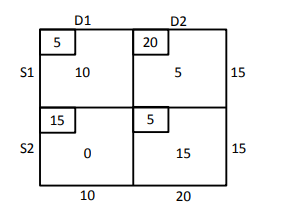
\includegraphics[width=0.75\columnwidth]{chapters/10/7/2/4/figs/fig.png}
 \end{center}
\caption{}
\label{fig:10/7/2/4Fig1}
\end{figure}
\fi

\item Find the position vector of the mid point of the vector joining the points $\vec{P}$(2, 3, 4)
and $\vec{Q}$(4, 1, –2).
\\
\solution
		\begin{enumerate}[label=\thesubsection.\arabic*,ref=\thesubsection.\theenumi]
\item Find the coordinates of the point which divides the join of $(-1,7) $ and $ (4,-3)$ in the ratio 2:3.
	\\
		\solution
	\input{chapters/10/7/2/1/section.tex}
\item Find the coordinates of the point $\vec{R}$ on the line segment joining the points $\vec{P}(-1,3)$ and $\vec{Q}(2,5)$ such that $PR=\frac{3}{5}PQ$.
\item Find the ratio in which the point $\vec{P}\brak{\frac{3}{4},\frac{5}{12}}$ divides the line segment joining the points $\vec{A}\brak{\frac{1}{2},\frac{3}{2}}$ and $ \vec{B}(2,-5)$.
\item Find the coordinates of the point which divides the line segment joining the points $(4,-3)$ and $(8,5)$ in the ratio $3:1$ internally.
\item Find the coordinates of the point $\vec{P}$ on $AD$ such that $AP : PD = 2 : 1$.
\item If the point $\vec{P} (2, 1)$ lies on the line segment joining points $\vec{A} (4, 2)$  and $ \vec{B} (8, 4)$,
then
\begin{enumerate}
	\item $AP =\frac{1}{3}{AB}$ 
\item ${AP}={PE}$
\item ${PB}=\frac{1}{3}{AB}$
\item${AP}=\frac{1}{2}{AB}$
 \end{enumerate}
\item Find the ratio in which the line segment joining the points $(-3,10)$  and  $(6,-8)$  is divided by $ (-1,6)$.
	\\
		\solution
	\input{chapters/10/7/2/4/section.tex}
\item Find the position vector of the mid point of the vector joining the points $\vec{P}$(2, 3, 4)
and $\vec{Q}$(4, 1, –2).
\\
\solution
		\input{chapters/12/10/2/16/section.tex}
\item Let $\vec{A}(4, 2), \vec{B}(6, 5)$  and $ \vec{C}(1, 4)$ be the vertices of $\triangle ABC$.
\begin{enumerate}
\item If $\vec{A}$ and  $\vec{B}$ are $(-2,-2)$ and  $(2,-4)$, respectively, find the coordinates of $\vec{P}$ such that $AP= \frac {3}{7}AB$  and $ \vec{P}$ lies on the line segment $AB$.
	\\
		\solution
	\input{chapters/10/7/2/8/section.tex}
\item Find the coordinates of the points which divide the line segment joining $A(-2,2)$  and  $\vec{B}(2,8)$ into four equal parts.
	\\
		\solution
	\input{chapters/10/7/2/9/section.tex}
\item In what ratio does the point $(-4,6)$ divide the line segment joining the points $\vec{A}(-6,0)$ and $\vec{B}(3,-8)$?
\item Given that $\vec{P}(3,2,-4), \vec{Q}(5,4,-6)$ and $\vec{R}(9,8,-10)$ are collinear. Find the ratio in which $\vec{Q}$ divides $PR$.
\item Points $\vec{A}(-6,10),\vec{B}(-4,6)$  and  $\vec{C}(3,-8)$ are collinear such that $AB=  \frac{2}{9}AC$.
\item The point which divides the line segment joining the points $\vec{P} (7, –6) $  and  $\vec{Q}(3, 4)$ in the 
ratio 1 : 2 internally lies in  which quadrant?
\item Find the coordinates of the points of trisection of the line segment joining $(4,-1)$  and  $(-2,3)$.
	\\
		\solution
	\input{chapters/10/7/2/2/section.tex}
\item Find the coordinates of the points which trisect the line segment joining the points $\vec{P}(4,2,-6)$ and $\vec{Q}(10,-16,6)$.
\item Find the coordinates of the points of trisection (i.e. points dividing to three equal parts) of the line segment joining the points $\vec{A}(2,-2)$ and $\vec{B}(-7,4)$.
\item Point $\vec{P}(5,-3)$ is one of the two points of trisection of line segment joining the points $\vec{A}(7,-2)$ and $\vec{B}(1,-5)$
\item Find the position vector of a point $\vec{R}$ which divides the line joining two points $\vec{P}$
and $\vec{Q}$ whose position vectors are $\hat{i}+2\hat{j}-\hat{k}$ and $-\hat{i}+\hat{j}+\hat{k}$ respectively, in the
ratio 2 : 1
\begin{enumerate}
    \item  internally
    \item  externally
\end{enumerate}
%\solution
%		\input{chapters/12/10/2/15/section.tex}
\item Find the coordinates of the point which divides the line segment joining the points which divides the line segment joining  the points $(-2,3,5)$ and $(1,-4,6)$ in the ratio 
\begin{enumerate}
\item $2:3$ internally,
\item $2:3$ externally
\end{enumerate}
\item Find the coordinates of the point which divides the line segment joining the points $(1,-2,3)$ and $(3,4,-5)$ in the ratio $2:3$
\begin{enumerate}
\item internally, and
\item externally
\end{enumerate}
\item Consider two points $\vec{P}$ and $\vec{Q}$ with position vectors $\overrightarrow{OP} = 3\overrightarrow{a}-2\overrightarrow{b}$ and $\overrightarrow{OQ}=\overrightarrow{a}+\overrightarrow{b}$. Find the position vector of a point $\vec{R}$ which divides the line joining $\vec{P}$ and $\vec{Q}$ in the ratio $2:1$, 
\begin{enumerate}
\item internally, and 
\item externally.
\end{enumerate}
\item The median from $\vec{A}$ meets $BC$ at $\vec{D}$. Find the coordinates of the point $\vec{D}$.
\item Find the coordinates of points $\vec{Q}$ and $\vec{R}$ on medians $BE$ and $CF$ respectively such that $BQ : QE = 2 : 1$  and  $CR : RF = 2 : 1$.
\item What do you observe?
\item If $\vec{A}, \vec{B}$ and $\vec{C}$  are the vertices of $\triangle ABC$, find the coordinates of the centroid of the triangle.
\end{enumerate}
\solution
	\input{chapters/10/7/4/7/section.tex}
\item If $\vec{P}(9a-2,-b)$ divides line segment joining $\vec{A}(3a+1,-3)$ and $\vec{B}(8a,5)$ in the ratio 3:1, find the values of $a$ and $b$.
\item Find the position vector of a point $\vec{R}$ which divides the line joining two points $\vec{P}$ and $\vec{Q}$ whose position vectors are $2\vec{a}+\vec{b}$ and $\vec{a}-3\vec{b}$ externally in the ratio $1:2$.
\item The position vector of the point which divides the join of points 2$\vec{a}$-3$\vec{b}$ $\text{and}$ $\vec{a}+\vec{b}$ in the ratio 3:1 is \rule{1cm}{0.1pt}.
\item If $\vec{a}$ and $\vec{b}$ are the postion vectors of $\vec{A}$ and $\vec{B}$, respectively, find the position vector of a point $\vec{C}$ in $BA$ produced such that $BC=1.5BA$.
\item Find the position vector of a point $\vec{R}$ which divides the line joining two points $\vec{P}$ and $\vec{Q}$ whose position vectors are $(2\vec{a}+\vec{b})$ and $(\vec{a}-3\vec{b})$
externally in the ratio 1 : 2. Also, show that $\vec{P}$ is the mid point of the line segment $RQ$.
\end{enumerate}

\item Let $\vec{A}(4, 2), \vec{B}(6, 5)$  and $ \vec{C}(1, 4)$ be the vertices of $\triangle ABC$.
\begin{enumerate}
\item If $\vec{A}$ and  $\vec{B}$ are $(-2,-2)$ and  $(2,-4)$, respectively, find the coordinates of $\vec{P}$ such that $AP= \frac {3}{7}AB$  and $ \vec{P}$ lies on the line segment $AB$.
	\\
		\solution
	\begin{enumerate}[label=\thesubsection.\arabic*,ref=\thesubsection.\theenumi]
\item Find the coordinates of the point which divides the join of $(-1,7) $ and $ (4,-3)$ in the ratio 2:3.
	\\
		\solution
	\input{chapters/10/7/2/1/section.tex}
\item Find the coordinates of the point $\vec{R}$ on the line segment joining the points $\vec{P}(-1,3)$ and $\vec{Q}(2,5)$ such that $PR=\frac{3}{5}PQ$.
\item Find the ratio in which the point $\vec{P}\brak{\frac{3}{4},\frac{5}{12}}$ divides the line segment joining the points $\vec{A}\brak{\frac{1}{2},\frac{3}{2}}$ and $ \vec{B}(2,-5)$.
\item Find the coordinates of the point which divides the line segment joining the points $(4,-3)$ and $(8,5)$ in the ratio $3:1$ internally.
\item Find the coordinates of the point $\vec{P}$ on $AD$ such that $AP : PD = 2 : 1$.
\item If the point $\vec{P} (2, 1)$ lies on the line segment joining points $\vec{A} (4, 2)$  and $ \vec{B} (8, 4)$,
then
\begin{enumerate}
	\item $AP =\frac{1}{3}{AB}$ 
\item ${AP}={PE}$
\item ${PB}=\frac{1}{3}{AB}$
\item${AP}=\frac{1}{2}{AB}$
 \end{enumerate}
\item Find the ratio in which the line segment joining the points $(-3,10)$  and  $(6,-8)$  is divided by $ (-1,6)$.
	\\
		\solution
	\input{chapters/10/7/2/4/section.tex}
\item Find the position vector of the mid point of the vector joining the points $\vec{P}$(2, 3, 4)
and $\vec{Q}$(4, 1, –2).
\\
\solution
		\input{chapters/12/10/2/16/section.tex}
\item Let $\vec{A}(4, 2), \vec{B}(6, 5)$  and $ \vec{C}(1, 4)$ be the vertices of $\triangle ABC$.
\begin{enumerate}
\item If $\vec{A}$ and  $\vec{B}$ are $(-2,-2)$ and  $(2,-4)$, respectively, find the coordinates of $\vec{P}$ such that $AP= \frac {3}{7}AB$  and $ \vec{P}$ lies on the line segment $AB$.
	\\
		\solution
	\input{chapters/10/7/2/8/section.tex}
\item Find the coordinates of the points which divide the line segment joining $A(-2,2)$  and  $\vec{B}(2,8)$ into four equal parts.
	\\
		\solution
	\input{chapters/10/7/2/9/section.tex}
\item In what ratio does the point $(-4,6)$ divide the line segment joining the points $\vec{A}(-6,0)$ and $\vec{B}(3,-8)$?
\item Given that $\vec{P}(3,2,-4), \vec{Q}(5,4,-6)$ and $\vec{R}(9,8,-10)$ are collinear. Find the ratio in which $\vec{Q}$ divides $PR$.
\item Points $\vec{A}(-6,10),\vec{B}(-4,6)$  and  $\vec{C}(3,-8)$ are collinear such that $AB=  \frac{2}{9}AC$.
\item The point which divides the line segment joining the points $\vec{P} (7, –6) $  and  $\vec{Q}(3, 4)$ in the 
ratio 1 : 2 internally lies in  which quadrant?
\item Find the coordinates of the points of trisection of the line segment joining $(4,-1)$  and  $(-2,3)$.
	\\
		\solution
	\input{chapters/10/7/2/2/section.tex}
\item Find the coordinates of the points which trisect the line segment joining the points $\vec{P}(4,2,-6)$ and $\vec{Q}(10,-16,6)$.
\item Find the coordinates of the points of trisection (i.e. points dividing to three equal parts) of the line segment joining the points $\vec{A}(2,-2)$ and $\vec{B}(-7,4)$.
\item Point $\vec{P}(5,-3)$ is one of the two points of trisection of line segment joining the points $\vec{A}(7,-2)$ and $\vec{B}(1,-5)$
\item Find the position vector of a point $\vec{R}$ which divides the line joining two points $\vec{P}$
and $\vec{Q}$ whose position vectors are $\hat{i}+2\hat{j}-\hat{k}$ and $-\hat{i}+\hat{j}+\hat{k}$ respectively, in the
ratio 2 : 1
\begin{enumerate}
    \item  internally
    \item  externally
\end{enumerate}
%\solution
%		\input{chapters/12/10/2/15/section.tex}
\item Find the coordinates of the point which divides the line segment joining the points which divides the line segment joining  the points $(-2,3,5)$ and $(1,-4,6)$ in the ratio 
\begin{enumerate}
\item $2:3$ internally,
\item $2:3$ externally
\end{enumerate}
\item Find the coordinates of the point which divides the line segment joining the points $(1,-2,3)$ and $(3,4,-5)$ in the ratio $2:3$
\begin{enumerate}
\item internally, and
\item externally
\end{enumerate}
\item Consider two points $\vec{P}$ and $\vec{Q}$ with position vectors $\overrightarrow{OP} = 3\overrightarrow{a}-2\overrightarrow{b}$ and $\overrightarrow{OQ}=\overrightarrow{a}+\overrightarrow{b}$. Find the position vector of a point $\vec{R}$ which divides the line joining $\vec{P}$ and $\vec{Q}$ in the ratio $2:1$, 
\begin{enumerate}
\item internally, and 
\item externally.
\end{enumerate}
\item The median from $\vec{A}$ meets $BC$ at $\vec{D}$. Find the coordinates of the point $\vec{D}$.
\item Find the coordinates of points $\vec{Q}$ and $\vec{R}$ on medians $BE$ and $CF$ respectively such that $BQ : QE = 2 : 1$  and  $CR : RF = 2 : 1$.
\item What do you observe?
\item If $\vec{A}, \vec{B}$ and $\vec{C}$  are the vertices of $\triangle ABC$, find the coordinates of the centroid of the triangle.
\end{enumerate}
\solution
	\input{chapters/10/7/4/7/section.tex}
\item If $\vec{P}(9a-2,-b)$ divides line segment joining $\vec{A}(3a+1,-3)$ and $\vec{B}(8a,5)$ in the ratio 3:1, find the values of $a$ and $b$.
\item Find the position vector of a point $\vec{R}$ which divides the line joining two points $\vec{P}$ and $\vec{Q}$ whose position vectors are $2\vec{a}+\vec{b}$ and $\vec{a}-3\vec{b}$ externally in the ratio $1:2$.
\item The position vector of the point which divides the join of points 2$\vec{a}$-3$\vec{b}$ $\text{and}$ $\vec{a}+\vec{b}$ in the ratio 3:1 is \rule{1cm}{0.1pt}.
\item If $\vec{a}$ and $\vec{b}$ are the postion vectors of $\vec{A}$ and $\vec{B}$, respectively, find the position vector of a point $\vec{C}$ in $BA$ produced such that $BC=1.5BA$.
\item Find the position vector of a point $\vec{R}$ which divides the line joining two points $\vec{P}$ and $\vec{Q}$ whose position vectors are $(2\vec{a}+\vec{b})$ and $(\vec{a}-3\vec{b})$
externally in the ratio 1 : 2. Also, show that $\vec{P}$ is the mid point of the line segment $RQ$.
\end{enumerate}

\item Find the coordinates of the points which divide the line segment joining $A(-2,2)$  and  $\vec{B}(2,8)$ into four equal parts.
	\\
		\solution
	\begin{enumerate}[label=\thesubsection.\arabic*,ref=\thesubsection.\theenumi]
\item Find the coordinates of the point which divides the join of $(-1,7) $ and $ (4,-3)$ in the ratio 2:3.
	\\
		\solution
	\input{chapters/10/7/2/1/section.tex}
\item Find the coordinates of the point $\vec{R}$ on the line segment joining the points $\vec{P}(-1,3)$ and $\vec{Q}(2,5)$ such that $PR=\frac{3}{5}PQ$.
\item Find the ratio in which the point $\vec{P}\brak{\frac{3}{4},\frac{5}{12}}$ divides the line segment joining the points $\vec{A}\brak{\frac{1}{2},\frac{3}{2}}$ and $ \vec{B}(2,-5)$.
\item Find the coordinates of the point which divides the line segment joining the points $(4,-3)$ and $(8,5)$ in the ratio $3:1$ internally.
\item Find the coordinates of the point $\vec{P}$ on $AD$ such that $AP : PD = 2 : 1$.
\item If the point $\vec{P} (2, 1)$ lies on the line segment joining points $\vec{A} (4, 2)$  and $ \vec{B} (8, 4)$,
then
\begin{enumerate}
	\item $AP =\frac{1}{3}{AB}$ 
\item ${AP}={PE}$
\item ${PB}=\frac{1}{3}{AB}$
\item${AP}=\frac{1}{2}{AB}$
 \end{enumerate}
\item Find the ratio in which the line segment joining the points $(-3,10)$  and  $(6,-8)$  is divided by $ (-1,6)$.
	\\
		\solution
	\input{chapters/10/7/2/4/section.tex}
\item Find the position vector of the mid point of the vector joining the points $\vec{P}$(2, 3, 4)
and $\vec{Q}$(4, 1, –2).
\\
\solution
		\input{chapters/12/10/2/16/section.tex}
\item Let $\vec{A}(4, 2), \vec{B}(6, 5)$  and $ \vec{C}(1, 4)$ be the vertices of $\triangle ABC$.
\begin{enumerate}
\item If $\vec{A}$ and  $\vec{B}$ are $(-2,-2)$ and  $(2,-4)$, respectively, find the coordinates of $\vec{P}$ such that $AP= \frac {3}{7}AB$  and $ \vec{P}$ lies on the line segment $AB$.
	\\
		\solution
	\input{chapters/10/7/2/8/section.tex}
\item Find the coordinates of the points which divide the line segment joining $A(-2,2)$  and  $\vec{B}(2,8)$ into four equal parts.
	\\
		\solution
	\input{chapters/10/7/2/9/section.tex}
\item In what ratio does the point $(-4,6)$ divide the line segment joining the points $\vec{A}(-6,0)$ and $\vec{B}(3,-8)$?
\item Given that $\vec{P}(3,2,-4), \vec{Q}(5,4,-6)$ and $\vec{R}(9,8,-10)$ are collinear. Find the ratio in which $\vec{Q}$ divides $PR$.
\item Points $\vec{A}(-6,10),\vec{B}(-4,6)$  and  $\vec{C}(3,-8)$ are collinear such that $AB=  \frac{2}{9}AC$.
\item The point which divides the line segment joining the points $\vec{P} (7, –6) $  and  $\vec{Q}(3, 4)$ in the 
ratio 1 : 2 internally lies in  which quadrant?
\item Find the coordinates of the points of trisection of the line segment joining $(4,-1)$  and  $(-2,3)$.
	\\
		\solution
	\input{chapters/10/7/2/2/section.tex}
\item Find the coordinates of the points which trisect the line segment joining the points $\vec{P}(4,2,-6)$ and $\vec{Q}(10,-16,6)$.
\item Find the coordinates of the points of trisection (i.e. points dividing to three equal parts) of the line segment joining the points $\vec{A}(2,-2)$ and $\vec{B}(-7,4)$.
\item Point $\vec{P}(5,-3)$ is one of the two points of trisection of line segment joining the points $\vec{A}(7,-2)$ and $\vec{B}(1,-5)$
\item Find the position vector of a point $\vec{R}$ which divides the line joining two points $\vec{P}$
and $\vec{Q}$ whose position vectors are $\hat{i}+2\hat{j}-\hat{k}$ and $-\hat{i}+\hat{j}+\hat{k}$ respectively, in the
ratio 2 : 1
\begin{enumerate}
    \item  internally
    \item  externally
\end{enumerate}
%\solution
%		\input{chapters/12/10/2/15/section.tex}
\item Find the coordinates of the point which divides the line segment joining the points which divides the line segment joining  the points $(-2,3,5)$ and $(1,-4,6)$ in the ratio 
\begin{enumerate}
\item $2:3$ internally,
\item $2:3$ externally
\end{enumerate}
\item Find the coordinates of the point which divides the line segment joining the points $(1,-2,3)$ and $(3,4,-5)$ in the ratio $2:3$
\begin{enumerate}
\item internally, and
\item externally
\end{enumerate}
\item Consider two points $\vec{P}$ and $\vec{Q}$ with position vectors $\overrightarrow{OP} = 3\overrightarrow{a}-2\overrightarrow{b}$ and $\overrightarrow{OQ}=\overrightarrow{a}+\overrightarrow{b}$. Find the position vector of a point $\vec{R}$ which divides the line joining $\vec{P}$ and $\vec{Q}$ in the ratio $2:1$, 
\begin{enumerate}
\item internally, and 
\item externally.
\end{enumerate}
\item The median from $\vec{A}$ meets $BC$ at $\vec{D}$. Find the coordinates of the point $\vec{D}$.
\item Find the coordinates of points $\vec{Q}$ and $\vec{R}$ on medians $BE$ and $CF$ respectively such that $BQ : QE = 2 : 1$  and  $CR : RF = 2 : 1$.
\item What do you observe?
\item If $\vec{A}, \vec{B}$ and $\vec{C}$  are the vertices of $\triangle ABC$, find the coordinates of the centroid of the triangle.
\end{enumerate}
\solution
	\input{chapters/10/7/4/7/section.tex}
\item If $\vec{P}(9a-2,-b)$ divides line segment joining $\vec{A}(3a+1,-3)$ and $\vec{B}(8a,5)$ in the ratio 3:1, find the values of $a$ and $b$.
\item Find the position vector of a point $\vec{R}$ which divides the line joining two points $\vec{P}$ and $\vec{Q}$ whose position vectors are $2\vec{a}+\vec{b}$ and $\vec{a}-3\vec{b}$ externally in the ratio $1:2$.
\item The position vector of the point which divides the join of points 2$\vec{a}$-3$\vec{b}$ $\text{and}$ $\vec{a}+\vec{b}$ in the ratio 3:1 is \rule{1cm}{0.1pt}.
\item If $\vec{a}$ and $\vec{b}$ are the postion vectors of $\vec{A}$ and $\vec{B}$, respectively, find the position vector of a point $\vec{C}$ in $BA$ produced such that $BC=1.5BA$.
\item Find the position vector of a point $\vec{R}$ which divides the line joining two points $\vec{P}$ and $\vec{Q}$ whose position vectors are $(2\vec{a}+\vec{b})$ and $(\vec{a}-3\vec{b})$
externally in the ratio 1 : 2. Also, show that $\vec{P}$ is the mid point of the line segment $RQ$.
\end{enumerate}

\item In what ratio does the point $(-4,6)$ divide the line segment joining the points $\vec{A}(-6,0)$ and $\vec{B}(3,-8)$?
\item Given that $\vec{P}(3,2,-4), \vec{Q}(5,4,-6)$ and $\vec{R}(9,8,-10)$ are collinear. Find the ratio in which $\vec{Q}$ divides $PR$.
\item Points $\vec{A}(-6,10),\vec{B}(-4,6)$  and  $\vec{C}(3,-8)$ are collinear such that $AB=  \frac{2}{9}AC$.
\item The point which divides the line segment joining the points $\vec{P} (7, –6) $  and  $\vec{Q}(3, 4)$ in the 
ratio 1 : 2 internally lies in  which quadrant?
\item Find the coordinates of the points of trisection of the line segment joining $(4,-1)$  and  $(-2,3)$.
	\\
		\solution
	Using section formula,
\begin{align}
\vec{R}=\frac{1}{1+\frac{1}{2}}\brak{\myvec{4\\-1}+\frac{1}{2}\myvec{-2\\3}}
=\myvec{2\\ \frac{1}{3}}\\
\vec{S}=\frac{1}{1+\frac{2}{1}}\brak{\myvec{4\\-1}+\frac{2}{1}\myvec{-2\\3}}
=\myvec{0\\ \frac{5}{3}}
\end{align}
which are the desired points of trisection.
\iffalse
See
		\figref{fig:chapters/10/7/2/2/Figure}
\begin{figure}[H]
\centering
\includegraphics[width=0.75\columnwidth]{chapters/10/7/2/2/figs/dj.pdf}
\caption{}
		\label{fig:chapters/10/7/2/2/Figure}
\end{figure}
\fi

\item Find the coordinates of the points which trisect the line segment joining the points $\vec{P}(4,2,-6)$ and $\vec{Q}(10,-16,6)$.
\item Find the coordinates of the points of trisection (i.e. points dividing to three equal parts) of the line segment joining the points $\vec{A}(2,-2)$ and $\vec{B}(-7,4)$.
\item Point $\vec{P}(5,-3)$ is one of the two points of trisection of line segment joining the points $\vec{A}(7,-2)$ and $\vec{B}(1,-5)$
\item Find the position vector of a point $\vec{R}$ which divides the line joining two points $\vec{P}$
and $\vec{Q}$ whose position vectors are $\hat{i}+2\hat{j}-\hat{k}$ and $-\hat{i}+\hat{j}+\hat{k}$ respectively, in the
ratio 2 : 1
\begin{enumerate}
    \item  internally
    \item  externally
\end{enumerate}
%\solution
%		\begin{enumerate}[label=\thesubsection.\arabic*,ref=\thesubsection.\theenumi]
\item Find the coordinates of the point which divides the join of $(-1,7) $ and $ (4,-3)$ in the ratio 2:3.
	\\
		\solution
	\input{chapters/10/7/2/1/section.tex}
\item Find the coordinates of the point $\vec{R}$ on the line segment joining the points $\vec{P}(-1,3)$ and $\vec{Q}(2,5)$ such that $PR=\frac{3}{5}PQ$.
\item Find the ratio in which the point $\vec{P}\brak{\frac{3}{4},\frac{5}{12}}$ divides the line segment joining the points $\vec{A}\brak{\frac{1}{2},\frac{3}{2}}$ and $ \vec{B}(2,-5)$.
\item Find the coordinates of the point which divides the line segment joining the points $(4,-3)$ and $(8,5)$ in the ratio $3:1$ internally.
\item Find the coordinates of the point $\vec{P}$ on $AD$ such that $AP : PD = 2 : 1$.
\item If the point $\vec{P} (2, 1)$ lies on the line segment joining points $\vec{A} (4, 2)$  and $ \vec{B} (8, 4)$,
then
\begin{enumerate}
	\item $AP =\frac{1}{3}{AB}$ 
\item ${AP}={PE}$
\item ${PB}=\frac{1}{3}{AB}$
\item${AP}=\frac{1}{2}{AB}$
 \end{enumerate}
\item Find the ratio in which the line segment joining the points $(-3,10)$  and  $(6,-8)$  is divided by $ (-1,6)$.
	\\
		\solution
	\input{chapters/10/7/2/4/section.tex}
\item Find the position vector of the mid point of the vector joining the points $\vec{P}$(2, 3, 4)
and $\vec{Q}$(4, 1, –2).
\\
\solution
		\input{chapters/12/10/2/16/section.tex}
\item Let $\vec{A}(4, 2), \vec{B}(6, 5)$  and $ \vec{C}(1, 4)$ be the vertices of $\triangle ABC$.
\begin{enumerate}
\item If $\vec{A}$ and  $\vec{B}$ are $(-2,-2)$ and  $(2,-4)$, respectively, find the coordinates of $\vec{P}$ such that $AP= \frac {3}{7}AB$  and $ \vec{P}$ lies on the line segment $AB$.
	\\
		\solution
	\input{chapters/10/7/2/8/section.tex}
\item Find the coordinates of the points which divide the line segment joining $A(-2,2)$  and  $\vec{B}(2,8)$ into four equal parts.
	\\
		\solution
	\input{chapters/10/7/2/9/section.tex}
\item In what ratio does the point $(-4,6)$ divide the line segment joining the points $\vec{A}(-6,0)$ and $\vec{B}(3,-8)$?
\item Given that $\vec{P}(3,2,-4), \vec{Q}(5,4,-6)$ and $\vec{R}(9,8,-10)$ are collinear. Find the ratio in which $\vec{Q}$ divides $PR$.
\item Points $\vec{A}(-6,10),\vec{B}(-4,6)$  and  $\vec{C}(3,-8)$ are collinear such that $AB=  \frac{2}{9}AC$.
\item The point which divides the line segment joining the points $\vec{P} (7, –6) $  and  $\vec{Q}(3, 4)$ in the 
ratio 1 : 2 internally lies in  which quadrant?
\item Find the coordinates of the points of trisection of the line segment joining $(4,-1)$  and  $(-2,3)$.
	\\
		\solution
	\input{chapters/10/7/2/2/section.tex}
\item Find the coordinates of the points which trisect the line segment joining the points $\vec{P}(4,2,-6)$ and $\vec{Q}(10,-16,6)$.
\item Find the coordinates of the points of trisection (i.e. points dividing to three equal parts) of the line segment joining the points $\vec{A}(2,-2)$ and $\vec{B}(-7,4)$.
\item Point $\vec{P}(5,-3)$ is one of the two points of trisection of line segment joining the points $\vec{A}(7,-2)$ and $\vec{B}(1,-5)$
\item Find the position vector of a point $\vec{R}$ which divides the line joining two points $\vec{P}$
and $\vec{Q}$ whose position vectors are $\hat{i}+2\hat{j}-\hat{k}$ and $-\hat{i}+\hat{j}+\hat{k}$ respectively, in the
ratio 2 : 1
\begin{enumerate}
    \item  internally
    \item  externally
\end{enumerate}
%\solution
%		\input{chapters/12/10/2/15/section.tex}
\item Find the coordinates of the point which divides the line segment joining the points which divides the line segment joining  the points $(-2,3,5)$ and $(1,-4,6)$ in the ratio 
\begin{enumerate}
\item $2:3$ internally,
\item $2:3$ externally
\end{enumerate}
\item Find the coordinates of the point which divides the line segment joining the points $(1,-2,3)$ and $(3,4,-5)$ in the ratio $2:3$
\begin{enumerate}
\item internally, and
\item externally
\end{enumerate}
\item Consider two points $\vec{P}$ and $\vec{Q}$ with position vectors $\overrightarrow{OP} = 3\overrightarrow{a}-2\overrightarrow{b}$ and $\overrightarrow{OQ}=\overrightarrow{a}+\overrightarrow{b}$. Find the position vector of a point $\vec{R}$ which divides the line joining $\vec{P}$ and $\vec{Q}$ in the ratio $2:1$, 
\begin{enumerate}
\item internally, and 
\item externally.
\end{enumerate}
\item The median from $\vec{A}$ meets $BC$ at $\vec{D}$. Find the coordinates of the point $\vec{D}$.
\item Find the coordinates of points $\vec{Q}$ and $\vec{R}$ on medians $BE$ and $CF$ respectively such that $BQ : QE = 2 : 1$  and  $CR : RF = 2 : 1$.
\item What do you observe?
\item If $\vec{A}, \vec{B}$ and $\vec{C}$  are the vertices of $\triangle ABC$, find the coordinates of the centroid of the triangle.
\end{enumerate}
\solution
	\input{chapters/10/7/4/7/section.tex}
\item If $\vec{P}(9a-2,-b)$ divides line segment joining $\vec{A}(3a+1,-3)$ and $\vec{B}(8a,5)$ in the ratio 3:1, find the values of $a$ and $b$.
\item Find the position vector of a point $\vec{R}$ which divides the line joining two points $\vec{P}$ and $\vec{Q}$ whose position vectors are $2\vec{a}+\vec{b}$ and $\vec{a}-3\vec{b}$ externally in the ratio $1:2$.
\item The position vector of the point which divides the join of points 2$\vec{a}$-3$\vec{b}$ $\text{and}$ $\vec{a}+\vec{b}$ in the ratio 3:1 is \rule{1cm}{0.1pt}.
\item If $\vec{a}$ and $\vec{b}$ are the postion vectors of $\vec{A}$ and $\vec{B}$, respectively, find the position vector of a point $\vec{C}$ in $BA$ produced such that $BC=1.5BA$.
\item Find the position vector of a point $\vec{R}$ which divides the line joining two points $\vec{P}$ and $\vec{Q}$ whose position vectors are $(2\vec{a}+\vec{b})$ and $(\vec{a}-3\vec{b})$
externally in the ratio 1 : 2. Also, show that $\vec{P}$ is the mid point of the line segment $RQ$.
\end{enumerate}

\item Find the coordinates of the point which divides the line segment joining the points which divides the line segment joining  the points $(-2,3,5)$ and $(1,-4,6)$ in the ratio 
\begin{enumerate}
\item $2:3$ internally,
\item $2:3$ externally
\end{enumerate}
\item Find the coordinates of the point which divides the line segment joining the points $(1,-2,3)$ and $(3,4,-5)$ in the ratio $2:3$
\begin{enumerate}
\item internally, and
\item externally
\end{enumerate}
\item Consider two points $\vec{P}$ and $\vec{Q}$ with position vectors $\overrightarrow{OP} = 3\overrightarrow{a}-2\overrightarrow{b}$ and $\overrightarrow{OQ}=\overrightarrow{a}+\overrightarrow{b}$. Find the position vector of a point $\vec{R}$ which divides the line joining $\vec{P}$ and $\vec{Q}$ in the ratio $2:1$, 
\begin{enumerate}
\item internally, and 
\item externally.
\end{enumerate}
\item The median from $\vec{A}$ meets $BC$ at $\vec{D}$. Find the coordinates of the point $\vec{D}$.
\item Find the coordinates of points $\vec{Q}$ and $\vec{R}$ on medians $BE$ and $CF$ respectively such that $BQ : QE = 2 : 1$  and  $CR : RF = 2 : 1$.
\item What do you observe?
\item If $\vec{A}, \vec{B}$ and $\vec{C}$  are the vertices of $\triangle ABC$, find the coordinates of the centroid of the triangle.
\end{enumerate}
\solution
	\begin{enumerate}[label=\thesubsection.\arabic*,ref=\thesubsection.\theenumi]
\item Find the coordinates of the point which divides the join of $(-1,7) $ and $ (4,-3)$ in the ratio 2:3.
	\\
		\solution
	\input{chapters/10/7/2/1/section.tex}
\item Find the coordinates of the point $\vec{R}$ on the line segment joining the points $\vec{P}(-1,3)$ and $\vec{Q}(2,5)$ such that $PR=\frac{3}{5}PQ$.
\item Find the ratio in which the point $\vec{P}\brak{\frac{3}{4},\frac{5}{12}}$ divides the line segment joining the points $\vec{A}\brak{\frac{1}{2},\frac{3}{2}}$ and $ \vec{B}(2,-5)$.
\item Find the coordinates of the point which divides the line segment joining the points $(4,-3)$ and $(8,5)$ in the ratio $3:1$ internally.
\item Find the coordinates of the point $\vec{P}$ on $AD$ such that $AP : PD = 2 : 1$.
\item If the point $\vec{P} (2, 1)$ lies on the line segment joining points $\vec{A} (4, 2)$  and $ \vec{B} (8, 4)$,
then
\begin{enumerate}
	\item $AP =\frac{1}{3}{AB}$ 
\item ${AP}={PE}$
\item ${PB}=\frac{1}{3}{AB}$
\item${AP}=\frac{1}{2}{AB}$
 \end{enumerate}
\item Find the ratio in which the line segment joining the points $(-3,10)$  and  $(6,-8)$  is divided by $ (-1,6)$.
	\\
		\solution
	\input{chapters/10/7/2/4/section.tex}
\item Find the position vector of the mid point of the vector joining the points $\vec{P}$(2, 3, 4)
and $\vec{Q}$(4, 1, –2).
\\
\solution
		\input{chapters/12/10/2/16/section.tex}
\item Let $\vec{A}(4, 2), \vec{B}(6, 5)$  and $ \vec{C}(1, 4)$ be the vertices of $\triangle ABC$.
\begin{enumerate}
\item If $\vec{A}$ and  $\vec{B}$ are $(-2,-2)$ and  $(2,-4)$, respectively, find the coordinates of $\vec{P}$ such that $AP= \frac {3}{7}AB$  and $ \vec{P}$ lies on the line segment $AB$.
	\\
		\solution
	\input{chapters/10/7/2/8/section.tex}
\item Find the coordinates of the points which divide the line segment joining $A(-2,2)$  and  $\vec{B}(2,8)$ into four equal parts.
	\\
		\solution
	\input{chapters/10/7/2/9/section.tex}
\item In what ratio does the point $(-4,6)$ divide the line segment joining the points $\vec{A}(-6,0)$ and $\vec{B}(3,-8)$?
\item Given that $\vec{P}(3,2,-4), \vec{Q}(5,4,-6)$ and $\vec{R}(9,8,-10)$ are collinear. Find the ratio in which $\vec{Q}$ divides $PR$.
\item Points $\vec{A}(-6,10),\vec{B}(-4,6)$  and  $\vec{C}(3,-8)$ are collinear such that $AB=  \frac{2}{9}AC$.
\item The point which divides the line segment joining the points $\vec{P} (7, –6) $  and  $\vec{Q}(3, 4)$ in the 
ratio 1 : 2 internally lies in  which quadrant?
\item Find the coordinates of the points of trisection of the line segment joining $(4,-1)$  and  $(-2,3)$.
	\\
		\solution
	\input{chapters/10/7/2/2/section.tex}
\item Find the coordinates of the points which trisect the line segment joining the points $\vec{P}(4,2,-6)$ and $\vec{Q}(10,-16,6)$.
\item Find the coordinates of the points of trisection (i.e. points dividing to three equal parts) of the line segment joining the points $\vec{A}(2,-2)$ and $\vec{B}(-7,4)$.
\item Point $\vec{P}(5,-3)$ is one of the two points of trisection of line segment joining the points $\vec{A}(7,-2)$ and $\vec{B}(1,-5)$
\item Find the position vector of a point $\vec{R}$ which divides the line joining two points $\vec{P}$
and $\vec{Q}$ whose position vectors are $\hat{i}+2\hat{j}-\hat{k}$ and $-\hat{i}+\hat{j}+\hat{k}$ respectively, in the
ratio 2 : 1
\begin{enumerate}
    \item  internally
    \item  externally
\end{enumerate}
%\solution
%		\input{chapters/12/10/2/15/section.tex}
\item Find the coordinates of the point which divides the line segment joining the points which divides the line segment joining  the points $(-2,3,5)$ and $(1,-4,6)$ in the ratio 
\begin{enumerate}
\item $2:3$ internally,
\item $2:3$ externally
\end{enumerate}
\item Find the coordinates of the point which divides the line segment joining the points $(1,-2,3)$ and $(3,4,-5)$ in the ratio $2:3$
\begin{enumerate}
\item internally, and
\item externally
\end{enumerate}
\item Consider two points $\vec{P}$ and $\vec{Q}$ with position vectors $\overrightarrow{OP} = 3\overrightarrow{a}-2\overrightarrow{b}$ and $\overrightarrow{OQ}=\overrightarrow{a}+\overrightarrow{b}$. Find the position vector of a point $\vec{R}$ which divides the line joining $\vec{P}$ and $\vec{Q}$ in the ratio $2:1$, 
\begin{enumerate}
\item internally, and 
\item externally.
\end{enumerate}
\item The median from $\vec{A}$ meets $BC$ at $\vec{D}$. Find the coordinates of the point $\vec{D}$.
\item Find the coordinates of points $\vec{Q}$ and $\vec{R}$ on medians $BE$ and $CF$ respectively such that $BQ : QE = 2 : 1$  and  $CR : RF = 2 : 1$.
\item What do you observe?
\item If $\vec{A}, \vec{B}$ and $\vec{C}$  are the vertices of $\triangle ABC$, find the coordinates of the centroid of the triangle.
\end{enumerate}
\solution
	\input{chapters/10/7/4/7/section.tex}
\item If $\vec{P}(9a-2,-b)$ divides line segment joining $\vec{A}(3a+1,-3)$ and $\vec{B}(8a,5)$ in the ratio 3:1, find the values of $a$ and $b$.
\item Find the position vector of a point $\vec{R}$ which divides the line joining two points $\vec{P}$ and $\vec{Q}$ whose position vectors are $2\vec{a}+\vec{b}$ and $\vec{a}-3\vec{b}$ externally in the ratio $1:2$.
\item The position vector of the point which divides the join of points 2$\vec{a}$-3$\vec{b}$ $\text{and}$ $\vec{a}+\vec{b}$ in the ratio 3:1 is \rule{1cm}{0.1pt}.
\item If $\vec{a}$ and $\vec{b}$ are the postion vectors of $\vec{A}$ and $\vec{B}$, respectively, find the position vector of a point $\vec{C}$ in $BA$ produced such that $BC=1.5BA$.
\item Find the position vector of a point $\vec{R}$ which divides the line joining two points $\vec{P}$ and $\vec{Q}$ whose position vectors are $(2\vec{a}+\vec{b})$ and $(\vec{a}-3\vec{b})$
externally in the ratio 1 : 2. Also, show that $\vec{P}$ is the mid point of the line segment $RQ$.
\end{enumerate}

\item If $\vec{P}(9a-2,-b)$ divides line segment joining $\vec{A}(3a+1,-3)$ and $\vec{B}(8a,5)$ in the ratio 3:1, find the values of $a$ and $b$.
\item Find the position vector of a point $\vec{R}$ which divides the line joining two points $\vec{P}$ and $\vec{Q}$ whose position vectors are $2\vec{a}+\vec{b}$ and $\vec{a}-3\vec{b}$ externally in the ratio $1:2$.
\item The position vector of the point which divides the join of points 2$\vec{a}$-3$\vec{b}$ $\text{and}$ $\vec{a}+\vec{b}$ in the ratio 3:1 is \rule{1cm}{0.1pt}.
\item If $\vec{a}$ and $\vec{b}$ are the postion vectors of $\vec{A}$ and $\vec{B}$, respectively, find the position vector of a point $\vec{C}$ in $BA$ produced such that $BC=1.5BA$.
\item Find the position vector of a point $\vec{R}$ which divides the line joining two points $\vec{P}$ and $\vec{Q}$ whose position vectors are $(2\vec{a}+\vec{b})$ and $(\vec{a}-3\vec{b})$
externally in the ratio 1 : 2. Also, show that $\vec{P}$ is the mid point of the line segment $RQ$.
\end{enumerate}

\item Find the coordinates of the point which divides the line segment joining the points which divides the line segment joining  the points $(-2,3,5)$ and $(1,-4,6)$ in the ratio 
\begin{enumerate}
\item $2:3$ internally,
\item $2:3$ externally
\end{enumerate}
\item Find the coordinates of the point which divides the line segment joining the points $(1,-2,3)$ and $(3,4,-5)$ in the ratio $2:3$
\begin{enumerate}
\item internally, and
\item externally
\end{enumerate}
\item Consider two points $\vec{P}$ and $\vec{Q}$ with position vectors $\overrightarrow{OP} = 3\overrightarrow{a}-2\overrightarrow{b}$ and $\overrightarrow{OQ}=\overrightarrow{a}+\overrightarrow{b}$. Find the position vector of a point $\vec{R}$ which divides the line joining $\vec{P}$ and $\vec{Q}$ in the ratio $2:1$, 
\begin{enumerate}
\item internally, and 
\item externally.
\end{enumerate}
\item The median from $\vec{A}$ meets $BC$ at $\vec{D}$. Find the coordinates of the point $\vec{D}$.
\item Find the coordinates of points $\vec{Q}$ and $\vec{R}$ on medians $BE$ and $CF$ respectively such that $BQ : QE = 2 : 1$  and  $CR : RF = 2 : 1$.
\item What do you observe?
\item If $\vec{A}, \vec{B}$ and $\vec{C}$  are the vertices of $\triangle ABC$, find the coordinates of the centroid of the triangle.
\end{enumerate}
\solution
	\begin{enumerate}[label=\thesubsection.\arabic*,ref=\thesubsection.\theenumi]
\item Find the coordinates of the point which divides the join of $(-1,7) $ and $ (4,-3)$ in the ratio 2:3.
	\\
		\solution
	\begin{enumerate}[label=\thesubsection.\arabic*,ref=\thesubsection.\theenumi]
\item Find the coordinates of the point which divides the join of $(-1,7) $ and $ (4,-3)$ in the ratio 2:3.
	\\
		\solution
	\input{chapters/10/7/2/1/section.tex}
\item Find the coordinates of the point $\vec{R}$ on the line segment joining the points $\vec{P}(-1,3)$ and $\vec{Q}(2,5)$ such that $PR=\frac{3}{5}PQ$.
\item Find the ratio in which the point $\vec{P}\brak{\frac{3}{4},\frac{5}{12}}$ divides the line segment joining the points $\vec{A}\brak{\frac{1}{2},\frac{3}{2}}$ and $ \vec{B}(2,-5)$.
\item Find the coordinates of the point which divides the line segment joining the points $(4,-3)$ and $(8,5)$ in the ratio $3:1$ internally.
\item Find the coordinates of the point $\vec{P}$ on $AD$ such that $AP : PD = 2 : 1$.
\item If the point $\vec{P} (2, 1)$ lies on the line segment joining points $\vec{A} (4, 2)$  and $ \vec{B} (8, 4)$,
then
\begin{enumerate}
	\item $AP =\frac{1}{3}{AB}$ 
\item ${AP}={PE}$
\item ${PB}=\frac{1}{3}{AB}$
\item${AP}=\frac{1}{2}{AB}$
 \end{enumerate}
\item Find the ratio in which the line segment joining the points $(-3,10)$  and  $(6,-8)$  is divided by $ (-1,6)$.
	\\
		\solution
	\input{chapters/10/7/2/4/section.tex}
\item Find the position vector of the mid point of the vector joining the points $\vec{P}$(2, 3, 4)
and $\vec{Q}$(4, 1, –2).
\\
\solution
		\input{chapters/12/10/2/16/section.tex}
\item Let $\vec{A}(4, 2), \vec{B}(6, 5)$  and $ \vec{C}(1, 4)$ be the vertices of $\triangle ABC$.
\begin{enumerate}
\item If $\vec{A}$ and  $\vec{B}$ are $(-2,-2)$ and  $(2,-4)$, respectively, find the coordinates of $\vec{P}$ such that $AP= \frac {3}{7}AB$  and $ \vec{P}$ lies on the line segment $AB$.
	\\
		\solution
	\input{chapters/10/7/2/8/section.tex}
\item Find the coordinates of the points which divide the line segment joining $A(-2,2)$  and  $\vec{B}(2,8)$ into four equal parts.
	\\
		\solution
	\input{chapters/10/7/2/9/section.tex}
\item In what ratio does the point $(-4,6)$ divide the line segment joining the points $\vec{A}(-6,0)$ and $\vec{B}(3,-8)$?
\item Given that $\vec{P}(3,2,-4), \vec{Q}(5,4,-6)$ and $\vec{R}(9,8,-10)$ are collinear. Find the ratio in which $\vec{Q}$ divides $PR$.
\item Points $\vec{A}(-6,10),\vec{B}(-4,6)$  and  $\vec{C}(3,-8)$ are collinear such that $AB=  \frac{2}{9}AC$.
\item The point which divides the line segment joining the points $\vec{P} (7, –6) $  and  $\vec{Q}(3, 4)$ in the 
ratio 1 : 2 internally lies in  which quadrant?
\item Find the coordinates of the points of trisection of the line segment joining $(4,-1)$  and  $(-2,3)$.
	\\
		\solution
	\input{chapters/10/7/2/2/section.tex}
\item Find the coordinates of the points which trisect the line segment joining the points $\vec{P}(4,2,-6)$ and $\vec{Q}(10,-16,6)$.
\item Find the coordinates of the points of trisection (i.e. points dividing to three equal parts) of the line segment joining the points $\vec{A}(2,-2)$ and $\vec{B}(-7,4)$.
\item Point $\vec{P}(5,-3)$ is one of the two points of trisection of line segment joining the points $\vec{A}(7,-2)$ and $\vec{B}(1,-5)$
\item Find the position vector of a point $\vec{R}$ which divides the line joining two points $\vec{P}$
and $\vec{Q}$ whose position vectors are $\hat{i}+2\hat{j}-\hat{k}$ and $-\hat{i}+\hat{j}+\hat{k}$ respectively, in the
ratio 2 : 1
\begin{enumerate}
    \item  internally
    \item  externally
\end{enumerate}
%\solution
%		\input{chapters/12/10/2/15/section.tex}
\item Find the coordinates of the point which divides the line segment joining the points which divides the line segment joining  the points $(-2,3,5)$ and $(1,-4,6)$ in the ratio 
\begin{enumerate}
\item $2:3$ internally,
\item $2:3$ externally
\end{enumerate}
\item Find the coordinates of the point which divides the line segment joining the points $(1,-2,3)$ and $(3,4,-5)$ in the ratio $2:3$
\begin{enumerate}
\item internally, and
\item externally
\end{enumerate}
\item Consider two points $\vec{P}$ and $\vec{Q}$ with position vectors $\overrightarrow{OP} = 3\overrightarrow{a}-2\overrightarrow{b}$ and $\overrightarrow{OQ}=\overrightarrow{a}+\overrightarrow{b}$. Find the position vector of a point $\vec{R}$ which divides the line joining $\vec{P}$ and $\vec{Q}$ in the ratio $2:1$, 
\begin{enumerate}
\item internally, and 
\item externally.
\end{enumerate}
\item The median from $\vec{A}$ meets $BC$ at $\vec{D}$. Find the coordinates of the point $\vec{D}$.
\item Find the coordinates of points $\vec{Q}$ and $\vec{R}$ on medians $BE$ and $CF$ respectively such that $BQ : QE = 2 : 1$  and  $CR : RF = 2 : 1$.
\item What do you observe?
\item If $\vec{A}, \vec{B}$ and $\vec{C}$  are the vertices of $\triangle ABC$, find the coordinates of the centroid of the triangle.
\end{enumerate}
\solution
	\input{chapters/10/7/4/7/section.tex}
\item If $\vec{P}(9a-2,-b)$ divides line segment joining $\vec{A}(3a+1,-3)$ and $\vec{B}(8a,5)$ in the ratio 3:1, find the values of $a$ and $b$.
\item Find the position vector of a point $\vec{R}$ which divides the line joining two points $\vec{P}$ and $\vec{Q}$ whose position vectors are $2\vec{a}+\vec{b}$ and $\vec{a}-3\vec{b}$ externally in the ratio $1:2$.
\item The position vector of the point which divides the join of points 2$\vec{a}$-3$\vec{b}$ $\text{and}$ $\vec{a}+\vec{b}$ in the ratio 3:1 is \rule{1cm}{0.1pt}.
\item If $\vec{a}$ and $\vec{b}$ are the postion vectors of $\vec{A}$ and $\vec{B}$, respectively, find the position vector of a point $\vec{C}$ in $BA$ produced such that $BC=1.5BA$.
\item Find the position vector of a point $\vec{R}$ which divides the line joining two points $\vec{P}$ and $\vec{Q}$ whose position vectors are $(2\vec{a}+\vec{b})$ and $(\vec{a}-3\vec{b})$
externally in the ratio 1 : 2. Also, show that $\vec{P}$ is the mid point of the line segment $RQ$.
\end{enumerate}

\item Find the coordinates of the point $\vec{R}$ on the line segment joining the points $\vec{P}(-1,3)$ and $\vec{Q}(2,5)$ such that $PR=\frac{3}{5}PQ$.
\item Find the ratio in which the point $\vec{P}\brak{\frac{3}{4},\frac{5}{12}}$ divides the line segment joining the points $\vec{A}\brak{\frac{1}{2},\frac{3}{2}}$ and $ \vec{B}(2,-5)$.
\item Find the coordinates of the point which divides the line segment joining the points $(4,-3)$ and $(8,5)$ in the ratio $3:1$ internally.
\item Find the coordinates of the point $\vec{P}$ on $AD$ such that $AP : PD = 2 : 1$.
\item If the point $\vec{P} (2, 1)$ lies on the line segment joining points $\vec{A} (4, 2)$  and $ \vec{B} (8, 4)$,
then
\begin{enumerate}
	\item $AP =\frac{1}{3}{AB}$ 
\item ${AP}={PE}$
\item ${PB}=\frac{1}{3}{AB}$
\item${AP}=\frac{1}{2}{AB}$
 \end{enumerate}
\item Find the ratio in which the line segment joining the points $(-3,10)$  and  $(6,-8)$  is divided by $ (-1,6)$.
	\\
		\solution
	\iffalse
Using section formula,
\begin{align}
         \myvec{-1\\6} &=\frac{{\myvec{-3\\10}+k\myvec{6\\-8}}}{1+k}\\
	 \implies 7k\myvec{1 \\ -2} &= 2\myvec{1 \\ -2}
	 \\
	 \text{or, } k &= \frac{2}{7}.
\end{align}
\fi
In 
			\eqref{eq:section_formula-k}, substituting
			\begin{align}
				\vec{B} &= \myvec{-3\\10}, \vec{C} = \myvec{6\\-8}, \vec{D} = \myvec{-1\\6},
				\\
				k &= \frac{\myvec{-2 & 4}\myvec{-7 \\ 14}}{\norm{\myvec{-7 \\ 14}}^2} = \frac{2}{7}
			\end{align}
\iffalse
See \figref{fig:10/7/2/4Fig1}.
\begin{figure}[H]
 \begin{center}
  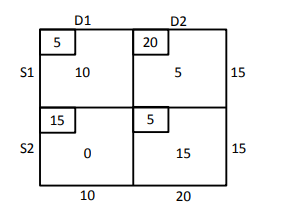
\includegraphics[width=0.75\columnwidth]{chapters/10/7/2/4/figs/fig.png}
 \end{center}
\caption{}
\label{fig:10/7/2/4Fig1}
\end{figure}
\fi

\item Find the position vector of the mid point of the vector joining the points $\vec{P}$(2, 3, 4)
and $\vec{Q}$(4, 1, –2).
\\
\solution
		\begin{enumerate}[label=\thesubsection.\arabic*,ref=\thesubsection.\theenumi]
\item Find the coordinates of the point which divides the join of $(-1,7) $ and $ (4,-3)$ in the ratio 2:3.
	\\
		\solution
	\input{chapters/10/7/2/1/section.tex}
\item Find the coordinates of the point $\vec{R}$ on the line segment joining the points $\vec{P}(-1,3)$ and $\vec{Q}(2,5)$ such that $PR=\frac{3}{5}PQ$.
\item Find the ratio in which the point $\vec{P}\brak{\frac{3}{4},\frac{5}{12}}$ divides the line segment joining the points $\vec{A}\brak{\frac{1}{2},\frac{3}{2}}$ and $ \vec{B}(2,-5)$.
\item Find the coordinates of the point which divides the line segment joining the points $(4,-3)$ and $(8,5)$ in the ratio $3:1$ internally.
\item Find the coordinates of the point $\vec{P}$ on $AD$ such that $AP : PD = 2 : 1$.
\item If the point $\vec{P} (2, 1)$ lies on the line segment joining points $\vec{A} (4, 2)$  and $ \vec{B} (8, 4)$,
then
\begin{enumerate}
	\item $AP =\frac{1}{3}{AB}$ 
\item ${AP}={PE}$
\item ${PB}=\frac{1}{3}{AB}$
\item${AP}=\frac{1}{2}{AB}$
 \end{enumerate}
\item Find the ratio in which the line segment joining the points $(-3,10)$  and  $(6,-8)$  is divided by $ (-1,6)$.
	\\
		\solution
	\input{chapters/10/7/2/4/section.tex}
\item Find the position vector of the mid point of the vector joining the points $\vec{P}$(2, 3, 4)
and $\vec{Q}$(4, 1, –2).
\\
\solution
		\input{chapters/12/10/2/16/section.tex}
\item Let $\vec{A}(4, 2), \vec{B}(6, 5)$  and $ \vec{C}(1, 4)$ be the vertices of $\triangle ABC$.
\begin{enumerate}
\item If $\vec{A}$ and  $\vec{B}$ are $(-2,-2)$ and  $(2,-4)$, respectively, find the coordinates of $\vec{P}$ such that $AP= \frac {3}{7}AB$  and $ \vec{P}$ lies on the line segment $AB$.
	\\
		\solution
	\input{chapters/10/7/2/8/section.tex}
\item Find the coordinates of the points which divide the line segment joining $A(-2,2)$  and  $\vec{B}(2,8)$ into four equal parts.
	\\
		\solution
	\input{chapters/10/7/2/9/section.tex}
\item In what ratio does the point $(-4,6)$ divide the line segment joining the points $\vec{A}(-6,0)$ and $\vec{B}(3,-8)$?
\item Given that $\vec{P}(3,2,-4), \vec{Q}(5,4,-6)$ and $\vec{R}(9,8,-10)$ are collinear. Find the ratio in which $\vec{Q}$ divides $PR$.
\item Points $\vec{A}(-6,10),\vec{B}(-4,6)$  and  $\vec{C}(3,-8)$ are collinear such that $AB=  \frac{2}{9}AC$.
\item The point which divides the line segment joining the points $\vec{P} (7, –6) $  and  $\vec{Q}(3, 4)$ in the 
ratio 1 : 2 internally lies in  which quadrant?
\item Find the coordinates of the points of trisection of the line segment joining $(4,-1)$  and  $(-2,3)$.
	\\
		\solution
	\input{chapters/10/7/2/2/section.tex}
\item Find the coordinates of the points which trisect the line segment joining the points $\vec{P}(4,2,-6)$ and $\vec{Q}(10,-16,6)$.
\item Find the coordinates of the points of trisection (i.e. points dividing to three equal parts) of the line segment joining the points $\vec{A}(2,-2)$ and $\vec{B}(-7,4)$.
\item Point $\vec{P}(5,-3)$ is one of the two points of trisection of line segment joining the points $\vec{A}(7,-2)$ and $\vec{B}(1,-5)$
\item Find the position vector of a point $\vec{R}$ which divides the line joining two points $\vec{P}$
and $\vec{Q}$ whose position vectors are $\hat{i}+2\hat{j}-\hat{k}$ and $-\hat{i}+\hat{j}+\hat{k}$ respectively, in the
ratio 2 : 1
\begin{enumerate}
    \item  internally
    \item  externally
\end{enumerate}
%\solution
%		\input{chapters/12/10/2/15/section.tex}
\item Find the coordinates of the point which divides the line segment joining the points which divides the line segment joining  the points $(-2,3,5)$ and $(1,-4,6)$ in the ratio 
\begin{enumerate}
\item $2:3$ internally,
\item $2:3$ externally
\end{enumerate}
\item Find the coordinates of the point which divides the line segment joining the points $(1,-2,3)$ and $(3,4,-5)$ in the ratio $2:3$
\begin{enumerate}
\item internally, and
\item externally
\end{enumerate}
\item Consider two points $\vec{P}$ and $\vec{Q}$ with position vectors $\overrightarrow{OP} = 3\overrightarrow{a}-2\overrightarrow{b}$ and $\overrightarrow{OQ}=\overrightarrow{a}+\overrightarrow{b}$. Find the position vector of a point $\vec{R}$ which divides the line joining $\vec{P}$ and $\vec{Q}$ in the ratio $2:1$, 
\begin{enumerate}
\item internally, and 
\item externally.
\end{enumerate}
\item The median from $\vec{A}$ meets $BC$ at $\vec{D}$. Find the coordinates of the point $\vec{D}$.
\item Find the coordinates of points $\vec{Q}$ and $\vec{R}$ on medians $BE$ and $CF$ respectively such that $BQ : QE = 2 : 1$  and  $CR : RF = 2 : 1$.
\item What do you observe?
\item If $\vec{A}, \vec{B}$ and $\vec{C}$  are the vertices of $\triangle ABC$, find the coordinates of the centroid of the triangle.
\end{enumerate}
\solution
	\input{chapters/10/7/4/7/section.tex}
\item If $\vec{P}(9a-2,-b)$ divides line segment joining $\vec{A}(3a+1,-3)$ and $\vec{B}(8a,5)$ in the ratio 3:1, find the values of $a$ and $b$.
\item Find the position vector of a point $\vec{R}$ which divides the line joining two points $\vec{P}$ and $\vec{Q}$ whose position vectors are $2\vec{a}+\vec{b}$ and $\vec{a}-3\vec{b}$ externally in the ratio $1:2$.
\item The position vector of the point which divides the join of points 2$\vec{a}$-3$\vec{b}$ $\text{and}$ $\vec{a}+\vec{b}$ in the ratio 3:1 is \rule{1cm}{0.1pt}.
\item If $\vec{a}$ and $\vec{b}$ are the postion vectors of $\vec{A}$ and $\vec{B}$, respectively, find the position vector of a point $\vec{C}$ in $BA$ produced such that $BC=1.5BA$.
\item Find the position vector of a point $\vec{R}$ which divides the line joining two points $\vec{P}$ and $\vec{Q}$ whose position vectors are $(2\vec{a}+\vec{b})$ and $(\vec{a}-3\vec{b})$
externally in the ratio 1 : 2. Also, show that $\vec{P}$ is the mid point of the line segment $RQ$.
\end{enumerate}

\item Let $\vec{A}(4, 2), \vec{B}(6, 5)$  and $ \vec{C}(1, 4)$ be the vertices of $\triangle ABC$.
\begin{enumerate}
\item If $\vec{A}$ and  $\vec{B}$ are $(-2,-2)$ and  $(2,-4)$, respectively, find the coordinates of $\vec{P}$ such that $AP= \frac {3}{7}AB$  and $ \vec{P}$ lies on the line segment $AB$.
	\\
		\solution
	\begin{enumerate}[label=\thesubsection.\arabic*,ref=\thesubsection.\theenumi]
\item Find the coordinates of the point which divides the join of $(-1,7) $ and $ (4,-3)$ in the ratio 2:3.
	\\
		\solution
	\input{chapters/10/7/2/1/section.tex}
\item Find the coordinates of the point $\vec{R}$ on the line segment joining the points $\vec{P}(-1,3)$ and $\vec{Q}(2,5)$ such that $PR=\frac{3}{5}PQ$.
\item Find the ratio in which the point $\vec{P}\brak{\frac{3}{4},\frac{5}{12}}$ divides the line segment joining the points $\vec{A}\brak{\frac{1}{2},\frac{3}{2}}$ and $ \vec{B}(2,-5)$.
\item Find the coordinates of the point which divides the line segment joining the points $(4,-3)$ and $(8,5)$ in the ratio $3:1$ internally.
\item Find the coordinates of the point $\vec{P}$ on $AD$ such that $AP : PD = 2 : 1$.
\item If the point $\vec{P} (2, 1)$ lies on the line segment joining points $\vec{A} (4, 2)$  and $ \vec{B} (8, 4)$,
then
\begin{enumerate}
	\item $AP =\frac{1}{3}{AB}$ 
\item ${AP}={PE}$
\item ${PB}=\frac{1}{3}{AB}$
\item${AP}=\frac{1}{2}{AB}$
 \end{enumerate}
\item Find the ratio in which the line segment joining the points $(-3,10)$  and  $(6,-8)$  is divided by $ (-1,6)$.
	\\
		\solution
	\input{chapters/10/7/2/4/section.tex}
\item Find the position vector of the mid point of the vector joining the points $\vec{P}$(2, 3, 4)
and $\vec{Q}$(4, 1, –2).
\\
\solution
		\input{chapters/12/10/2/16/section.tex}
\item Let $\vec{A}(4, 2), \vec{B}(6, 5)$  and $ \vec{C}(1, 4)$ be the vertices of $\triangle ABC$.
\begin{enumerate}
\item If $\vec{A}$ and  $\vec{B}$ are $(-2,-2)$ and  $(2,-4)$, respectively, find the coordinates of $\vec{P}$ such that $AP= \frac {3}{7}AB$  and $ \vec{P}$ lies on the line segment $AB$.
	\\
		\solution
	\input{chapters/10/7/2/8/section.tex}
\item Find the coordinates of the points which divide the line segment joining $A(-2,2)$  and  $\vec{B}(2,8)$ into four equal parts.
	\\
		\solution
	\input{chapters/10/7/2/9/section.tex}
\item In what ratio does the point $(-4,6)$ divide the line segment joining the points $\vec{A}(-6,0)$ and $\vec{B}(3,-8)$?
\item Given that $\vec{P}(3,2,-4), \vec{Q}(5,4,-6)$ and $\vec{R}(9,8,-10)$ are collinear. Find the ratio in which $\vec{Q}$ divides $PR$.
\item Points $\vec{A}(-6,10),\vec{B}(-4,6)$  and  $\vec{C}(3,-8)$ are collinear such that $AB=  \frac{2}{9}AC$.
\item The point which divides the line segment joining the points $\vec{P} (7, –6) $  and  $\vec{Q}(3, 4)$ in the 
ratio 1 : 2 internally lies in  which quadrant?
\item Find the coordinates of the points of trisection of the line segment joining $(4,-1)$  and  $(-2,3)$.
	\\
		\solution
	\input{chapters/10/7/2/2/section.tex}
\item Find the coordinates of the points which trisect the line segment joining the points $\vec{P}(4,2,-6)$ and $\vec{Q}(10,-16,6)$.
\item Find the coordinates of the points of trisection (i.e. points dividing to three equal parts) of the line segment joining the points $\vec{A}(2,-2)$ and $\vec{B}(-7,4)$.
\item Point $\vec{P}(5,-3)$ is one of the two points of trisection of line segment joining the points $\vec{A}(7,-2)$ and $\vec{B}(1,-5)$
\item Find the position vector of a point $\vec{R}$ which divides the line joining two points $\vec{P}$
and $\vec{Q}$ whose position vectors are $\hat{i}+2\hat{j}-\hat{k}$ and $-\hat{i}+\hat{j}+\hat{k}$ respectively, in the
ratio 2 : 1
\begin{enumerate}
    \item  internally
    \item  externally
\end{enumerate}
%\solution
%		\input{chapters/12/10/2/15/section.tex}
\item Find the coordinates of the point which divides the line segment joining the points which divides the line segment joining  the points $(-2,3,5)$ and $(1,-4,6)$ in the ratio 
\begin{enumerate}
\item $2:3$ internally,
\item $2:3$ externally
\end{enumerate}
\item Find the coordinates of the point which divides the line segment joining the points $(1,-2,3)$ and $(3,4,-5)$ in the ratio $2:3$
\begin{enumerate}
\item internally, and
\item externally
\end{enumerate}
\item Consider two points $\vec{P}$ and $\vec{Q}$ with position vectors $\overrightarrow{OP} = 3\overrightarrow{a}-2\overrightarrow{b}$ and $\overrightarrow{OQ}=\overrightarrow{a}+\overrightarrow{b}$. Find the position vector of a point $\vec{R}$ which divides the line joining $\vec{P}$ and $\vec{Q}$ in the ratio $2:1$, 
\begin{enumerate}
\item internally, and 
\item externally.
\end{enumerate}
\item The median from $\vec{A}$ meets $BC$ at $\vec{D}$. Find the coordinates of the point $\vec{D}$.
\item Find the coordinates of points $\vec{Q}$ and $\vec{R}$ on medians $BE$ and $CF$ respectively such that $BQ : QE = 2 : 1$  and  $CR : RF = 2 : 1$.
\item What do you observe?
\item If $\vec{A}, \vec{B}$ and $\vec{C}$  are the vertices of $\triangle ABC$, find the coordinates of the centroid of the triangle.
\end{enumerate}
\solution
	\input{chapters/10/7/4/7/section.tex}
\item If $\vec{P}(9a-2,-b)$ divides line segment joining $\vec{A}(3a+1,-3)$ and $\vec{B}(8a,5)$ in the ratio 3:1, find the values of $a$ and $b$.
\item Find the position vector of a point $\vec{R}$ which divides the line joining two points $\vec{P}$ and $\vec{Q}$ whose position vectors are $2\vec{a}+\vec{b}$ and $\vec{a}-3\vec{b}$ externally in the ratio $1:2$.
\item The position vector of the point which divides the join of points 2$\vec{a}$-3$\vec{b}$ $\text{and}$ $\vec{a}+\vec{b}$ in the ratio 3:1 is \rule{1cm}{0.1pt}.
\item If $\vec{a}$ and $\vec{b}$ are the postion vectors of $\vec{A}$ and $\vec{B}$, respectively, find the position vector of a point $\vec{C}$ in $BA$ produced such that $BC=1.5BA$.
\item Find the position vector of a point $\vec{R}$ which divides the line joining two points $\vec{P}$ and $\vec{Q}$ whose position vectors are $(2\vec{a}+\vec{b})$ and $(\vec{a}-3\vec{b})$
externally in the ratio 1 : 2. Also, show that $\vec{P}$ is the mid point of the line segment $RQ$.
\end{enumerate}

\item Find the coordinates of the points which divide the line segment joining $A(-2,2)$  and  $\vec{B}(2,8)$ into four equal parts.
	\\
		\solution
	\begin{enumerate}[label=\thesubsection.\arabic*,ref=\thesubsection.\theenumi]
\item Find the coordinates of the point which divides the join of $(-1,7) $ and $ (4,-3)$ in the ratio 2:3.
	\\
		\solution
	\input{chapters/10/7/2/1/section.tex}
\item Find the coordinates of the point $\vec{R}$ on the line segment joining the points $\vec{P}(-1,3)$ and $\vec{Q}(2,5)$ such that $PR=\frac{3}{5}PQ$.
\item Find the ratio in which the point $\vec{P}\brak{\frac{3}{4},\frac{5}{12}}$ divides the line segment joining the points $\vec{A}\brak{\frac{1}{2},\frac{3}{2}}$ and $ \vec{B}(2,-5)$.
\item Find the coordinates of the point which divides the line segment joining the points $(4,-3)$ and $(8,5)$ in the ratio $3:1$ internally.
\item Find the coordinates of the point $\vec{P}$ on $AD$ such that $AP : PD = 2 : 1$.
\item If the point $\vec{P} (2, 1)$ lies on the line segment joining points $\vec{A} (4, 2)$  and $ \vec{B} (8, 4)$,
then
\begin{enumerate}
	\item $AP =\frac{1}{3}{AB}$ 
\item ${AP}={PE}$
\item ${PB}=\frac{1}{3}{AB}$
\item${AP}=\frac{1}{2}{AB}$
 \end{enumerate}
\item Find the ratio in which the line segment joining the points $(-3,10)$  and  $(6,-8)$  is divided by $ (-1,6)$.
	\\
		\solution
	\input{chapters/10/7/2/4/section.tex}
\item Find the position vector of the mid point of the vector joining the points $\vec{P}$(2, 3, 4)
and $\vec{Q}$(4, 1, –2).
\\
\solution
		\input{chapters/12/10/2/16/section.tex}
\item Let $\vec{A}(4, 2), \vec{B}(6, 5)$  and $ \vec{C}(1, 4)$ be the vertices of $\triangle ABC$.
\begin{enumerate}
\item If $\vec{A}$ and  $\vec{B}$ are $(-2,-2)$ and  $(2,-4)$, respectively, find the coordinates of $\vec{P}$ such that $AP= \frac {3}{7}AB$  and $ \vec{P}$ lies on the line segment $AB$.
	\\
		\solution
	\input{chapters/10/7/2/8/section.tex}
\item Find the coordinates of the points which divide the line segment joining $A(-2,2)$  and  $\vec{B}(2,8)$ into four equal parts.
	\\
		\solution
	\input{chapters/10/7/2/9/section.tex}
\item In what ratio does the point $(-4,6)$ divide the line segment joining the points $\vec{A}(-6,0)$ and $\vec{B}(3,-8)$?
\item Given that $\vec{P}(3,2,-4), \vec{Q}(5,4,-6)$ and $\vec{R}(9,8,-10)$ are collinear. Find the ratio in which $\vec{Q}$ divides $PR$.
\item Points $\vec{A}(-6,10),\vec{B}(-4,6)$  and  $\vec{C}(3,-8)$ are collinear such that $AB=  \frac{2}{9}AC$.
\item The point which divides the line segment joining the points $\vec{P} (7, –6) $  and  $\vec{Q}(3, 4)$ in the 
ratio 1 : 2 internally lies in  which quadrant?
\item Find the coordinates of the points of trisection of the line segment joining $(4,-1)$  and  $(-2,3)$.
	\\
		\solution
	\input{chapters/10/7/2/2/section.tex}
\item Find the coordinates of the points which trisect the line segment joining the points $\vec{P}(4,2,-6)$ and $\vec{Q}(10,-16,6)$.
\item Find the coordinates of the points of trisection (i.e. points dividing to three equal parts) of the line segment joining the points $\vec{A}(2,-2)$ and $\vec{B}(-7,4)$.
\item Point $\vec{P}(5,-3)$ is one of the two points of trisection of line segment joining the points $\vec{A}(7,-2)$ and $\vec{B}(1,-5)$
\item Find the position vector of a point $\vec{R}$ which divides the line joining two points $\vec{P}$
and $\vec{Q}$ whose position vectors are $\hat{i}+2\hat{j}-\hat{k}$ and $-\hat{i}+\hat{j}+\hat{k}$ respectively, in the
ratio 2 : 1
\begin{enumerate}
    \item  internally
    \item  externally
\end{enumerate}
%\solution
%		\input{chapters/12/10/2/15/section.tex}
\item Find the coordinates of the point which divides the line segment joining the points which divides the line segment joining  the points $(-2,3,5)$ and $(1,-4,6)$ in the ratio 
\begin{enumerate}
\item $2:3$ internally,
\item $2:3$ externally
\end{enumerate}
\item Find the coordinates of the point which divides the line segment joining the points $(1,-2,3)$ and $(3,4,-5)$ in the ratio $2:3$
\begin{enumerate}
\item internally, and
\item externally
\end{enumerate}
\item Consider two points $\vec{P}$ and $\vec{Q}$ with position vectors $\overrightarrow{OP} = 3\overrightarrow{a}-2\overrightarrow{b}$ and $\overrightarrow{OQ}=\overrightarrow{a}+\overrightarrow{b}$. Find the position vector of a point $\vec{R}$ which divides the line joining $\vec{P}$ and $\vec{Q}$ in the ratio $2:1$, 
\begin{enumerate}
\item internally, and 
\item externally.
\end{enumerate}
\item The median from $\vec{A}$ meets $BC$ at $\vec{D}$. Find the coordinates of the point $\vec{D}$.
\item Find the coordinates of points $\vec{Q}$ and $\vec{R}$ on medians $BE$ and $CF$ respectively such that $BQ : QE = 2 : 1$  and  $CR : RF = 2 : 1$.
\item What do you observe?
\item If $\vec{A}, \vec{B}$ and $\vec{C}$  are the vertices of $\triangle ABC$, find the coordinates of the centroid of the triangle.
\end{enumerate}
\solution
	\input{chapters/10/7/4/7/section.tex}
\item If $\vec{P}(9a-2,-b)$ divides line segment joining $\vec{A}(3a+1,-3)$ and $\vec{B}(8a,5)$ in the ratio 3:1, find the values of $a$ and $b$.
\item Find the position vector of a point $\vec{R}$ which divides the line joining two points $\vec{P}$ and $\vec{Q}$ whose position vectors are $2\vec{a}+\vec{b}$ and $\vec{a}-3\vec{b}$ externally in the ratio $1:2$.
\item The position vector of the point which divides the join of points 2$\vec{a}$-3$\vec{b}$ $\text{and}$ $\vec{a}+\vec{b}$ in the ratio 3:1 is \rule{1cm}{0.1pt}.
\item If $\vec{a}$ and $\vec{b}$ are the postion vectors of $\vec{A}$ and $\vec{B}$, respectively, find the position vector of a point $\vec{C}$ in $BA$ produced such that $BC=1.5BA$.
\item Find the position vector of a point $\vec{R}$ which divides the line joining two points $\vec{P}$ and $\vec{Q}$ whose position vectors are $(2\vec{a}+\vec{b})$ and $(\vec{a}-3\vec{b})$
externally in the ratio 1 : 2. Also, show that $\vec{P}$ is the mid point of the line segment $RQ$.
\end{enumerate}

\item In what ratio does the point $(-4,6)$ divide the line segment joining the points $\vec{A}(-6,0)$ and $\vec{B}(3,-8)$?
\item Given that $\vec{P}(3,2,-4), \vec{Q}(5,4,-6)$ and $\vec{R}(9,8,-10)$ are collinear. Find the ratio in which $\vec{Q}$ divides $PR$.
\item Points $\vec{A}(-6,10),\vec{B}(-4,6)$  and  $\vec{C}(3,-8)$ are collinear such that $AB=  \frac{2}{9}AC$.
\item The point which divides the line segment joining the points $\vec{P} (7, –6) $  and  $\vec{Q}(3, 4)$ in the 
ratio 1 : 2 internally lies in  which quadrant?
\item Find the coordinates of the points of trisection of the line segment joining $(4,-1)$  and  $(-2,3)$.
	\\
		\solution
	Using section formula,
\begin{align}
\vec{R}=\frac{1}{1+\frac{1}{2}}\brak{\myvec{4\\-1}+\frac{1}{2}\myvec{-2\\3}}
=\myvec{2\\ \frac{1}{3}}\\
\vec{S}=\frac{1}{1+\frac{2}{1}}\brak{\myvec{4\\-1}+\frac{2}{1}\myvec{-2\\3}}
=\myvec{0\\ \frac{5}{3}}
\end{align}
which are the desired points of trisection.
\iffalse
See
		\figref{fig:chapters/10/7/2/2/Figure}
\begin{figure}[H]
\centering
\includegraphics[width=0.75\columnwidth]{chapters/10/7/2/2/figs/dj.pdf}
\caption{}
		\label{fig:chapters/10/7/2/2/Figure}
\end{figure}
\fi

\item Find the coordinates of the points which trisect the line segment joining the points $\vec{P}(4,2,-6)$ and $\vec{Q}(10,-16,6)$.
\item Find the coordinates of the points of trisection (i.e. points dividing to three equal parts) of the line segment joining the points $\vec{A}(2,-2)$ and $\vec{B}(-7,4)$.
\item Point $\vec{P}(5,-3)$ is one of the two points of trisection of line segment joining the points $\vec{A}(7,-2)$ and $\vec{B}(1,-5)$
\item Find the position vector of a point $\vec{R}$ which divides the line joining two points $\vec{P}$
and $\vec{Q}$ whose position vectors are $\hat{i}+2\hat{j}-\hat{k}$ and $-\hat{i}+\hat{j}+\hat{k}$ respectively, in the
ratio 2 : 1
\begin{enumerate}
    \item  internally
    \item  externally
\end{enumerate}
%\solution
%		\begin{enumerate}[label=\thesubsection.\arabic*,ref=\thesubsection.\theenumi]
\item Find the coordinates of the point which divides the join of $(-1,7) $ and $ (4,-3)$ in the ratio 2:3.
	\\
		\solution
	\input{chapters/10/7/2/1/section.tex}
\item Find the coordinates of the point $\vec{R}$ on the line segment joining the points $\vec{P}(-1,3)$ and $\vec{Q}(2,5)$ such that $PR=\frac{3}{5}PQ$.
\item Find the ratio in which the point $\vec{P}\brak{\frac{3}{4},\frac{5}{12}}$ divides the line segment joining the points $\vec{A}\brak{\frac{1}{2},\frac{3}{2}}$ and $ \vec{B}(2,-5)$.
\item Find the coordinates of the point which divides the line segment joining the points $(4,-3)$ and $(8,5)$ in the ratio $3:1$ internally.
\item Find the coordinates of the point $\vec{P}$ on $AD$ such that $AP : PD = 2 : 1$.
\item If the point $\vec{P} (2, 1)$ lies on the line segment joining points $\vec{A} (4, 2)$  and $ \vec{B} (8, 4)$,
then
\begin{enumerate}
	\item $AP =\frac{1}{3}{AB}$ 
\item ${AP}={PE}$
\item ${PB}=\frac{1}{3}{AB}$
\item${AP}=\frac{1}{2}{AB}$
 \end{enumerate}
\item Find the ratio in which the line segment joining the points $(-3,10)$  and  $(6,-8)$  is divided by $ (-1,6)$.
	\\
		\solution
	\input{chapters/10/7/2/4/section.tex}
\item Find the position vector of the mid point of the vector joining the points $\vec{P}$(2, 3, 4)
and $\vec{Q}$(4, 1, –2).
\\
\solution
		\input{chapters/12/10/2/16/section.tex}
\item Let $\vec{A}(4, 2), \vec{B}(6, 5)$  and $ \vec{C}(1, 4)$ be the vertices of $\triangle ABC$.
\begin{enumerate}
\item If $\vec{A}$ and  $\vec{B}$ are $(-2,-2)$ and  $(2,-4)$, respectively, find the coordinates of $\vec{P}$ such that $AP= \frac {3}{7}AB$  and $ \vec{P}$ lies on the line segment $AB$.
	\\
		\solution
	\input{chapters/10/7/2/8/section.tex}
\item Find the coordinates of the points which divide the line segment joining $A(-2,2)$  and  $\vec{B}(2,8)$ into four equal parts.
	\\
		\solution
	\input{chapters/10/7/2/9/section.tex}
\item In what ratio does the point $(-4,6)$ divide the line segment joining the points $\vec{A}(-6,0)$ and $\vec{B}(3,-8)$?
\item Given that $\vec{P}(3,2,-4), \vec{Q}(5,4,-6)$ and $\vec{R}(9,8,-10)$ are collinear. Find the ratio in which $\vec{Q}$ divides $PR$.
\item Points $\vec{A}(-6,10),\vec{B}(-4,6)$  and  $\vec{C}(3,-8)$ are collinear such that $AB=  \frac{2}{9}AC$.
\item The point which divides the line segment joining the points $\vec{P} (7, –6) $  and  $\vec{Q}(3, 4)$ in the 
ratio 1 : 2 internally lies in  which quadrant?
\item Find the coordinates of the points of trisection of the line segment joining $(4,-1)$  and  $(-2,3)$.
	\\
		\solution
	\input{chapters/10/7/2/2/section.tex}
\item Find the coordinates of the points which trisect the line segment joining the points $\vec{P}(4,2,-6)$ and $\vec{Q}(10,-16,6)$.
\item Find the coordinates of the points of trisection (i.e. points dividing to three equal parts) of the line segment joining the points $\vec{A}(2,-2)$ and $\vec{B}(-7,4)$.
\item Point $\vec{P}(5,-3)$ is one of the two points of trisection of line segment joining the points $\vec{A}(7,-2)$ and $\vec{B}(1,-5)$
\item Find the position vector of a point $\vec{R}$ which divides the line joining two points $\vec{P}$
and $\vec{Q}$ whose position vectors are $\hat{i}+2\hat{j}-\hat{k}$ and $-\hat{i}+\hat{j}+\hat{k}$ respectively, in the
ratio 2 : 1
\begin{enumerate}
    \item  internally
    \item  externally
\end{enumerate}
%\solution
%		\input{chapters/12/10/2/15/section.tex}
\item Find the coordinates of the point which divides the line segment joining the points which divides the line segment joining  the points $(-2,3,5)$ and $(1,-4,6)$ in the ratio 
\begin{enumerate}
\item $2:3$ internally,
\item $2:3$ externally
\end{enumerate}
\item Find the coordinates of the point which divides the line segment joining the points $(1,-2,3)$ and $(3,4,-5)$ in the ratio $2:3$
\begin{enumerate}
\item internally, and
\item externally
\end{enumerate}
\item Consider two points $\vec{P}$ and $\vec{Q}$ with position vectors $\overrightarrow{OP} = 3\overrightarrow{a}-2\overrightarrow{b}$ and $\overrightarrow{OQ}=\overrightarrow{a}+\overrightarrow{b}$. Find the position vector of a point $\vec{R}$ which divides the line joining $\vec{P}$ and $\vec{Q}$ in the ratio $2:1$, 
\begin{enumerate}
\item internally, and 
\item externally.
\end{enumerate}
\item The median from $\vec{A}$ meets $BC$ at $\vec{D}$. Find the coordinates of the point $\vec{D}$.
\item Find the coordinates of points $\vec{Q}$ and $\vec{R}$ on medians $BE$ and $CF$ respectively such that $BQ : QE = 2 : 1$  and  $CR : RF = 2 : 1$.
\item What do you observe?
\item If $\vec{A}, \vec{B}$ and $\vec{C}$  are the vertices of $\triangle ABC$, find the coordinates of the centroid of the triangle.
\end{enumerate}
\solution
	\input{chapters/10/7/4/7/section.tex}
\item If $\vec{P}(9a-2,-b)$ divides line segment joining $\vec{A}(3a+1,-3)$ and $\vec{B}(8a,5)$ in the ratio 3:1, find the values of $a$ and $b$.
\item Find the position vector of a point $\vec{R}$ which divides the line joining two points $\vec{P}$ and $\vec{Q}$ whose position vectors are $2\vec{a}+\vec{b}$ and $\vec{a}-3\vec{b}$ externally in the ratio $1:2$.
\item The position vector of the point which divides the join of points 2$\vec{a}$-3$\vec{b}$ $\text{and}$ $\vec{a}+\vec{b}$ in the ratio 3:1 is \rule{1cm}{0.1pt}.
\item If $\vec{a}$ and $\vec{b}$ are the postion vectors of $\vec{A}$ and $\vec{B}$, respectively, find the position vector of a point $\vec{C}$ in $BA$ produced such that $BC=1.5BA$.
\item Find the position vector of a point $\vec{R}$ which divides the line joining two points $\vec{P}$ and $\vec{Q}$ whose position vectors are $(2\vec{a}+\vec{b})$ and $(\vec{a}-3\vec{b})$
externally in the ratio 1 : 2. Also, show that $\vec{P}$ is the mid point of the line segment $RQ$.
\end{enumerate}

\item Find the coordinates of the point which divides the line segment joining the points which divides the line segment joining  the points $(-2,3,5)$ and $(1,-4,6)$ in the ratio 
\begin{enumerate}
\item $2:3$ internally,
\item $2:3$ externally
\end{enumerate}
\item Find the coordinates of the point which divides the line segment joining the points $(1,-2,3)$ and $(3,4,-5)$ in the ratio $2:3$
\begin{enumerate}
\item internally, and
\item externally
\end{enumerate}
\item Consider two points $\vec{P}$ and $\vec{Q}$ with position vectors $\overrightarrow{OP} = 3\overrightarrow{a}-2\overrightarrow{b}$ and $\overrightarrow{OQ}=\overrightarrow{a}+\overrightarrow{b}$. Find the position vector of a point $\vec{R}$ which divides the line joining $\vec{P}$ and $\vec{Q}$ in the ratio $2:1$, 
\begin{enumerate}
\item internally, and 
\item externally.
\end{enumerate}
\item The median from $\vec{A}$ meets $BC$ at $\vec{D}$. Find the coordinates of the point $\vec{D}$.
\item Find the coordinates of points $\vec{Q}$ and $\vec{R}$ on medians $BE$ and $CF$ respectively such that $BQ : QE = 2 : 1$  and  $CR : RF = 2 : 1$.
\item What do you observe?
\item If $\vec{A}, \vec{B}$ and $\vec{C}$  are the vertices of $\triangle ABC$, find the coordinates of the centroid of the triangle.
\end{enumerate}
\solution
	\begin{enumerate}[label=\thesubsection.\arabic*,ref=\thesubsection.\theenumi]
\item Find the coordinates of the point which divides the join of $(-1,7) $ and $ (4,-3)$ in the ratio 2:3.
	\\
		\solution
	\input{chapters/10/7/2/1/section.tex}
\item Find the coordinates of the point $\vec{R}$ on the line segment joining the points $\vec{P}(-1,3)$ and $\vec{Q}(2,5)$ such that $PR=\frac{3}{5}PQ$.
\item Find the ratio in which the point $\vec{P}\brak{\frac{3}{4},\frac{5}{12}}$ divides the line segment joining the points $\vec{A}\brak{\frac{1}{2},\frac{3}{2}}$ and $ \vec{B}(2,-5)$.
\item Find the coordinates of the point which divides the line segment joining the points $(4,-3)$ and $(8,5)$ in the ratio $3:1$ internally.
\item Find the coordinates of the point $\vec{P}$ on $AD$ such that $AP : PD = 2 : 1$.
\item If the point $\vec{P} (2, 1)$ lies on the line segment joining points $\vec{A} (4, 2)$  and $ \vec{B} (8, 4)$,
then
\begin{enumerate}
	\item $AP =\frac{1}{3}{AB}$ 
\item ${AP}={PE}$
\item ${PB}=\frac{1}{3}{AB}$
\item${AP}=\frac{1}{2}{AB}$
 \end{enumerate}
\item Find the ratio in which the line segment joining the points $(-3,10)$  and  $(6,-8)$  is divided by $ (-1,6)$.
	\\
		\solution
	\input{chapters/10/7/2/4/section.tex}
\item Find the position vector of the mid point of the vector joining the points $\vec{P}$(2, 3, 4)
and $\vec{Q}$(4, 1, –2).
\\
\solution
		\input{chapters/12/10/2/16/section.tex}
\item Let $\vec{A}(4, 2), \vec{B}(6, 5)$  and $ \vec{C}(1, 4)$ be the vertices of $\triangle ABC$.
\begin{enumerate}
\item If $\vec{A}$ and  $\vec{B}$ are $(-2,-2)$ and  $(2,-4)$, respectively, find the coordinates of $\vec{P}$ such that $AP= \frac {3}{7}AB$  and $ \vec{P}$ lies on the line segment $AB$.
	\\
		\solution
	\input{chapters/10/7/2/8/section.tex}
\item Find the coordinates of the points which divide the line segment joining $A(-2,2)$  and  $\vec{B}(2,8)$ into four equal parts.
	\\
		\solution
	\input{chapters/10/7/2/9/section.tex}
\item In what ratio does the point $(-4,6)$ divide the line segment joining the points $\vec{A}(-6,0)$ and $\vec{B}(3,-8)$?
\item Given that $\vec{P}(3,2,-4), \vec{Q}(5,4,-6)$ and $\vec{R}(9,8,-10)$ are collinear. Find the ratio in which $\vec{Q}$ divides $PR$.
\item Points $\vec{A}(-6,10),\vec{B}(-4,6)$  and  $\vec{C}(3,-8)$ are collinear such that $AB=  \frac{2}{9}AC$.
\item The point which divides the line segment joining the points $\vec{P} (7, –6) $  and  $\vec{Q}(3, 4)$ in the 
ratio 1 : 2 internally lies in  which quadrant?
\item Find the coordinates of the points of trisection of the line segment joining $(4,-1)$  and  $(-2,3)$.
	\\
		\solution
	\input{chapters/10/7/2/2/section.tex}
\item Find the coordinates of the points which trisect the line segment joining the points $\vec{P}(4,2,-6)$ and $\vec{Q}(10,-16,6)$.
\item Find the coordinates of the points of trisection (i.e. points dividing to three equal parts) of the line segment joining the points $\vec{A}(2,-2)$ and $\vec{B}(-7,4)$.
\item Point $\vec{P}(5,-3)$ is one of the two points of trisection of line segment joining the points $\vec{A}(7,-2)$ and $\vec{B}(1,-5)$
\item Find the position vector of a point $\vec{R}$ which divides the line joining two points $\vec{P}$
and $\vec{Q}$ whose position vectors are $\hat{i}+2\hat{j}-\hat{k}$ and $-\hat{i}+\hat{j}+\hat{k}$ respectively, in the
ratio 2 : 1
\begin{enumerate}
    \item  internally
    \item  externally
\end{enumerate}
%\solution
%		\input{chapters/12/10/2/15/section.tex}
\item Find the coordinates of the point which divides the line segment joining the points which divides the line segment joining  the points $(-2,3,5)$ and $(1,-4,6)$ in the ratio 
\begin{enumerate}
\item $2:3$ internally,
\item $2:3$ externally
\end{enumerate}
\item Find the coordinates of the point which divides the line segment joining the points $(1,-2,3)$ and $(3,4,-5)$ in the ratio $2:3$
\begin{enumerate}
\item internally, and
\item externally
\end{enumerate}
\item Consider two points $\vec{P}$ and $\vec{Q}$ with position vectors $\overrightarrow{OP} = 3\overrightarrow{a}-2\overrightarrow{b}$ and $\overrightarrow{OQ}=\overrightarrow{a}+\overrightarrow{b}$. Find the position vector of a point $\vec{R}$ which divides the line joining $\vec{P}$ and $\vec{Q}$ in the ratio $2:1$, 
\begin{enumerate}
\item internally, and 
\item externally.
\end{enumerate}
\item The median from $\vec{A}$ meets $BC$ at $\vec{D}$. Find the coordinates of the point $\vec{D}$.
\item Find the coordinates of points $\vec{Q}$ and $\vec{R}$ on medians $BE$ and $CF$ respectively such that $BQ : QE = 2 : 1$  and  $CR : RF = 2 : 1$.
\item What do you observe?
\item If $\vec{A}, \vec{B}$ and $\vec{C}$  are the vertices of $\triangle ABC$, find the coordinates of the centroid of the triangle.
\end{enumerate}
\solution
	\input{chapters/10/7/4/7/section.tex}
\item If $\vec{P}(9a-2,-b)$ divides line segment joining $\vec{A}(3a+1,-3)$ and $\vec{B}(8a,5)$ in the ratio 3:1, find the values of $a$ and $b$.
\item Find the position vector of a point $\vec{R}$ which divides the line joining two points $\vec{P}$ and $\vec{Q}$ whose position vectors are $2\vec{a}+\vec{b}$ and $\vec{a}-3\vec{b}$ externally in the ratio $1:2$.
\item The position vector of the point which divides the join of points 2$\vec{a}$-3$\vec{b}$ $\text{and}$ $\vec{a}+\vec{b}$ in the ratio 3:1 is \rule{1cm}{0.1pt}.
\item If $\vec{a}$ and $\vec{b}$ are the postion vectors of $\vec{A}$ and $\vec{B}$, respectively, find the position vector of a point $\vec{C}$ in $BA$ produced such that $BC=1.5BA$.
\item Find the position vector of a point $\vec{R}$ which divides the line joining two points $\vec{P}$ and $\vec{Q}$ whose position vectors are $(2\vec{a}+\vec{b})$ and $(\vec{a}-3\vec{b})$
externally in the ratio 1 : 2. Also, show that $\vec{P}$ is the mid point of the line segment $RQ$.
\end{enumerate}

\item If $\vec{P}(9a-2,-b)$ divides line segment joining $\vec{A}(3a+1,-3)$ and $\vec{B}(8a,5)$ in the ratio 3:1, find the values of $a$ and $b$.
\item Find the position vector of a point $\vec{R}$ which divides the line joining two points $\vec{P}$ and $\vec{Q}$ whose position vectors are $2\vec{a}+\vec{b}$ and $\vec{a}-3\vec{b}$ externally in the ratio $1:2$.
\item The position vector of the point which divides the join of points 2$\vec{a}$-3$\vec{b}$ $\text{and}$ $\vec{a}+\vec{b}$ in the ratio 3:1 is \rule{1cm}{0.1pt}.
\item If $\vec{a}$ and $\vec{b}$ are the postion vectors of $\vec{A}$ and $\vec{B}$, respectively, find the position vector of a point $\vec{C}$ in $BA$ produced such that $BC=1.5BA$.
\item Find the position vector of a point $\vec{R}$ which divides the line joining two points $\vec{P}$ and $\vec{Q}$ whose position vectors are $(2\vec{a}+\vec{b})$ and $(\vec{a}-3\vec{b})$
externally in the ratio 1 : 2. Also, show that $\vec{P}$ is the mid point of the line segment $RQ$.
\end{enumerate}

\item If $\vec{P}(9a-2,-b)$ divides line segment joining $\vec{A}(3a+1,-3)$ and $\vec{B}(8a,5)$ in the ratio 3:1, find the values of $a$ and $b$.
\item Find the position vector of a point $\vec{R}$ which divides the line joining two points $\vec{P}$ and $\vec{Q}$ whose position vectors are $2\vec{a}+\vec{b}$ and $\vec{a}-3\vec{b}$ externally in the ratio $1:2$.
\item The position vector of the point which divides the join of points 2$\vec{a}$-3$\vec{b}$ $\text{and}$ $\vec{a}+\vec{b}$ in the ratio 3:1 is \rule{1cm}{0.1pt}.
\item If $\vec{a}$ and $\vec{b}$ are the postion vectors of $\vec{A}$ and $\vec{B}$, respectively, find the position vector of a point $\vec{C}$ in $BA$ produced such that $BC=1.5BA$.
\item Find the position vector of a point $\vec{R}$ which divides the line joining two points $\vec{P}$ and $\vec{Q}$ whose position vectors are $(2\vec{a}+\vec{b})$ and $(\vec{a}-3\vec{b})$
externally in the ratio 1 : 2. Also, show that $\vec{P}$ is the mid point of the line segment $RQ$.
\end{enumerate}

\item Find the coordinates of the point $\vec{R}$ on the line segment joining the points $\vec{P}(-1,3)$ and $\vec{Q}(2,5)$ such that $PR=\frac{3}{5}PQ$.
\item Find the ratio in which the point $\vec{P}\brak{\frac{3}{4},\frac{5}{12}}$ divides the line segment joining the points $\vec{A}\brak{\frac{1}{2},\frac{3}{2}}$ and $ \vec{B}(2,-5)$.
\item Find the coordinates of the point which divides the line segment joining the points $(4,-3)$ and $(8,5)$ in the ratio $3:1$ internally.
\item Find the coordinates of the point $\vec{P}$ on $AD$ such that $AP : PD = 2 : 1$.
\item If the point $\vec{P} (2, 1)$ lies on the line segment joining points $\vec{A} (4, 2)$  and $ \vec{B} (8, 4)$,
then
\begin{enumerate}
	\item $AP =\frac{1}{3}{AB}$ 
\item ${AP}={PE}$
\item ${PB}=\frac{1}{3}{AB}$
\item${AP}=\frac{1}{2}{AB}$
 \end{enumerate}
\item Find the ratio in which the line segment joining the points $(-3,10)$  and  $(6,-8)$  is divided by $ (-1,6)$.
	\\
		\solution
	\iffalse
Using section formula,
\begin{align}
         \myvec{-1\\6} &=\frac{{\myvec{-3\\10}+k\myvec{6\\-8}}}{1+k}\\
	 \implies 7k\myvec{1 \\ -2} &= 2\myvec{1 \\ -2}
	 \\
	 \text{or, } k &= \frac{2}{7}.
\end{align}
\fi
In 
			\eqref{eq:section_formula-k}, substituting
			\begin{align}
				\vec{B} &= \myvec{-3\\10}, \vec{C} = \myvec{6\\-8}, \vec{D} = \myvec{-1\\6},
				\\
				k &= \frac{\myvec{-2 & 4}\myvec{-7 \\ 14}}{\norm{\myvec{-7 \\ 14}}^2} = \frac{2}{7}
			\end{align}
\iffalse
See \figref{fig:10/7/2/4Fig1}.
\begin{figure}[H]
 \begin{center}
  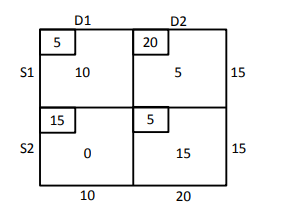
\includegraphics[width=0.75\columnwidth]{chapters/10/7/2/4/figs/fig.png}
 \end{center}
\caption{}
\label{fig:10/7/2/4Fig1}
\end{figure}
\fi

\item Find the position vector of the mid point of the vector joining the points $\vec{P}$(2, 3, 4)
and $\vec{Q}$(4, 1, –2).
\\
\solution
		\begin{enumerate}[label=\thesubsection.\arabic*,ref=\thesubsection.\theenumi]
\item Find the coordinates of the point which divides the join of $(-1,7) $ and $ (4,-3)$ in the ratio 2:3.
	\\
		\solution
	\begin{enumerate}[label=\thesubsection.\arabic*,ref=\thesubsection.\theenumi]
\item Find the coordinates of the point which divides the join of $(-1,7) $ and $ (4,-3)$ in the ratio 2:3.
	\\
		\solution
	\begin{enumerate}[label=\thesubsection.\arabic*,ref=\thesubsection.\theenumi]
\item Find the coordinates of the point which divides the join of $(-1,7) $ and $ (4,-3)$ in the ratio 2:3.
	\\
		\solution
	\input{chapters/10/7/2/1/section.tex}
\item Find the coordinates of the point $\vec{R}$ on the line segment joining the points $\vec{P}(-1,3)$ and $\vec{Q}(2,5)$ such that $PR=\frac{3}{5}PQ$.
\item Find the ratio in which the point $\vec{P}\brak{\frac{3}{4},\frac{5}{12}}$ divides the line segment joining the points $\vec{A}\brak{\frac{1}{2},\frac{3}{2}}$ and $ \vec{B}(2,-5)$.
\item Find the coordinates of the point which divides the line segment joining the points $(4,-3)$ and $(8,5)$ in the ratio $3:1$ internally.
\item Find the coordinates of the point $\vec{P}$ on $AD$ such that $AP : PD = 2 : 1$.
\item If the point $\vec{P} (2, 1)$ lies on the line segment joining points $\vec{A} (4, 2)$  and $ \vec{B} (8, 4)$,
then
\begin{enumerate}
	\item $AP =\frac{1}{3}{AB}$ 
\item ${AP}={PE}$
\item ${PB}=\frac{1}{3}{AB}$
\item${AP}=\frac{1}{2}{AB}$
 \end{enumerate}
\item Find the ratio in which the line segment joining the points $(-3,10)$  and  $(6,-8)$  is divided by $ (-1,6)$.
	\\
		\solution
	\input{chapters/10/7/2/4/section.tex}
\item Find the position vector of the mid point of the vector joining the points $\vec{P}$(2, 3, 4)
and $\vec{Q}$(4, 1, –2).
\\
\solution
		\input{chapters/12/10/2/16/section.tex}
\item Let $\vec{A}(4, 2), \vec{B}(6, 5)$  and $ \vec{C}(1, 4)$ be the vertices of $\triangle ABC$.
\begin{enumerate}
\item If $\vec{A}$ and  $\vec{B}$ are $(-2,-2)$ and  $(2,-4)$, respectively, find the coordinates of $\vec{P}$ such that $AP= \frac {3}{7}AB$  and $ \vec{P}$ lies on the line segment $AB$.
	\\
		\solution
	\input{chapters/10/7/2/8/section.tex}
\item Find the coordinates of the points which divide the line segment joining $A(-2,2)$  and  $\vec{B}(2,8)$ into four equal parts.
	\\
		\solution
	\input{chapters/10/7/2/9/section.tex}
\item In what ratio does the point $(-4,6)$ divide the line segment joining the points $\vec{A}(-6,0)$ and $\vec{B}(3,-8)$?
\item Given that $\vec{P}(3,2,-4), \vec{Q}(5,4,-6)$ and $\vec{R}(9,8,-10)$ are collinear. Find the ratio in which $\vec{Q}$ divides $PR$.
\item Points $\vec{A}(-6,10),\vec{B}(-4,6)$  and  $\vec{C}(3,-8)$ are collinear such that $AB=  \frac{2}{9}AC$.
\item The point which divides the line segment joining the points $\vec{P} (7, –6) $  and  $\vec{Q}(3, 4)$ in the 
ratio 1 : 2 internally lies in  which quadrant?
\item Find the coordinates of the points of trisection of the line segment joining $(4,-1)$  and  $(-2,3)$.
	\\
		\solution
	\input{chapters/10/7/2/2/section.tex}
\item Find the coordinates of the points which trisect the line segment joining the points $\vec{P}(4,2,-6)$ and $\vec{Q}(10,-16,6)$.
\item Find the coordinates of the points of trisection (i.e. points dividing to three equal parts) of the line segment joining the points $\vec{A}(2,-2)$ and $\vec{B}(-7,4)$.
\item Point $\vec{P}(5,-3)$ is one of the two points of trisection of line segment joining the points $\vec{A}(7,-2)$ and $\vec{B}(1,-5)$
\item Find the position vector of a point $\vec{R}$ which divides the line joining two points $\vec{P}$
and $\vec{Q}$ whose position vectors are $\hat{i}+2\hat{j}-\hat{k}$ and $-\hat{i}+\hat{j}+\hat{k}$ respectively, in the
ratio 2 : 1
\begin{enumerate}
    \item  internally
    \item  externally
\end{enumerate}
%\solution
%		\input{chapters/12/10/2/15/section.tex}
\item Find the coordinates of the point which divides the line segment joining the points which divides the line segment joining  the points $(-2,3,5)$ and $(1,-4,6)$ in the ratio 
\begin{enumerate}
\item $2:3$ internally,
\item $2:3$ externally
\end{enumerate}
\item Find the coordinates of the point which divides the line segment joining the points $(1,-2,3)$ and $(3,4,-5)$ in the ratio $2:3$
\begin{enumerate}
\item internally, and
\item externally
\end{enumerate}
\item Consider two points $\vec{P}$ and $\vec{Q}$ with position vectors $\overrightarrow{OP} = 3\overrightarrow{a}-2\overrightarrow{b}$ and $\overrightarrow{OQ}=\overrightarrow{a}+\overrightarrow{b}$. Find the position vector of a point $\vec{R}$ which divides the line joining $\vec{P}$ and $\vec{Q}$ in the ratio $2:1$, 
\begin{enumerate}
\item internally, and 
\item externally.
\end{enumerate}
\item The median from $\vec{A}$ meets $BC$ at $\vec{D}$. Find the coordinates of the point $\vec{D}$.
\item Find the coordinates of points $\vec{Q}$ and $\vec{R}$ on medians $BE$ and $CF$ respectively such that $BQ : QE = 2 : 1$  and  $CR : RF = 2 : 1$.
\item What do you observe?
\item If $\vec{A}, \vec{B}$ and $\vec{C}$  are the vertices of $\triangle ABC$, find the coordinates of the centroid of the triangle.
\end{enumerate}
\solution
	\input{chapters/10/7/4/7/section.tex}
\item If $\vec{P}(9a-2,-b)$ divides line segment joining $\vec{A}(3a+1,-3)$ and $\vec{B}(8a,5)$ in the ratio 3:1, find the values of $a$ and $b$.
\item Find the position vector of a point $\vec{R}$ which divides the line joining two points $\vec{P}$ and $\vec{Q}$ whose position vectors are $2\vec{a}+\vec{b}$ and $\vec{a}-3\vec{b}$ externally in the ratio $1:2$.
\item The position vector of the point which divides the join of points 2$\vec{a}$-3$\vec{b}$ $\text{and}$ $\vec{a}+\vec{b}$ in the ratio 3:1 is \rule{1cm}{0.1pt}.
\item If $\vec{a}$ and $\vec{b}$ are the postion vectors of $\vec{A}$ and $\vec{B}$, respectively, find the position vector of a point $\vec{C}$ in $BA$ produced such that $BC=1.5BA$.
\item Find the position vector of a point $\vec{R}$ which divides the line joining two points $\vec{P}$ and $\vec{Q}$ whose position vectors are $(2\vec{a}+\vec{b})$ and $(\vec{a}-3\vec{b})$
externally in the ratio 1 : 2. Also, show that $\vec{P}$ is the mid point of the line segment $RQ$.
\end{enumerate}

\item Find the coordinates of the point $\vec{R}$ on the line segment joining the points $\vec{P}(-1,3)$ and $\vec{Q}(2,5)$ such that $PR=\frac{3}{5}PQ$.
\item Find the ratio in which the point $\vec{P}\brak{\frac{3}{4},\frac{5}{12}}$ divides the line segment joining the points $\vec{A}\brak{\frac{1}{2},\frac{3}{2}}$ and $ \vec{B}(2,-5)$.
\item Find the coordinates of the point which divides the line segment joining the points $(4,-3)$ and $(8,5)$ in the ratio $3:1$ internally.
\item Find the coordinates of the point $\vec{P}$ on $AD$ such that $AP : PD = 2 : 1$.
\item If the point $\vec{P} (2, 1)$ lies on the line segment joining points $\vec{A} (4, 2)$  and $ \vec{B} (8, 4)$,
then
\begin{enumerate}
	\item $AP =\frac{1}{3}{AB}$ 
\item ${AP}={PE}$
\item ${PB}=\frac{1}{3}{AB}$
\item${AP}=\frac{1}{2}{AB}$
 \end{enumerate}
\item Find the ratio in which the line segment joining the points $(-3,10)$  and  $(6,-8)$  is divided by $ (-1,6)$.
	\\
		\solution
	\iffalse
Using section formula,
\begin{align}
         \myvec{-1\\6} &=\frac{{\myvec{-3\\10}+k\myvec{6\\-8}}}{1+k}\\
	 \implies 7k\myvec{1 \\ -2} &= 2\myvec{1 \\ -2}
	 \\
	 \text{or, } k &= \frac{2}{7}.
\end{align}
\fi
In 
			\eqref{eq:section_formula-k}, substituting
			\begin{align}
				\vec{B} &= \myvec{-3\\10}, \vec{C} = \myvec{6\\-8}, \vec{D} = \myvec{-1\\6},
				\\
				k &= \frac{\myvec{-2 & 4}\myvec{-7 \\ 14}}{\norm{\myvec{-7 \\ 14}}^2} = \frac{2}{7}
			\end{align}
\iffalse
See \figref{fig:10/7/2/4Fig1}.
\begin{figure}[H]
 \begin{center}
  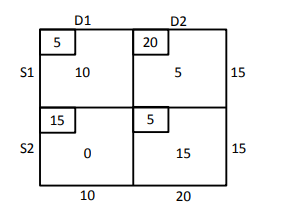
\includegraphics[width=0.75\columnwidth]{chapters/10/7/2/4/figs/fig.png}
 \end{center}
\caption{}
\label{fig:10/7/2/4Fig1}
\end{figure}
\fi

\item Find the position vector of the mid point of the vector joining the points $\vec{P}$(2, 3, 4)
and $\vec{Q}$(4, 1, –2).
\\
\solution
		\begin{enumerate}[label=\thesubsection.\arabic*,ref=\thesubsection.\theenumi]
\item Find the coordinates of the point which divides the join of $(-1,7) $ and $ (4,-3)$ in the ratio 2:3.
	\\
		\solution
	\input{chapters/10/7/2/1/section.tex}
\item Find the coordinates of the point $\vec{R}$ on the line segment joining the points $\vec{P}(-1,3)$ and $\vec{Q}(2,5)$ such that $PR=\frac{3}{5}PQ$.
\item Find the ratio in which the point $\vec{P}\brak{\frac{3}{4},\frac{5}{12}}$ divides the line segment joining the points $\vec{A}\brak{\frac{1}{2},\frac{3}{2}}$ and $ \vec{B}(2,-5)$.
\item Find the coordinates of the point which divides the line segment joining the points $(4,-3)$ and $(8,5)$ in the ratio $3:1$ internally.
\item Find the coordinates of the point $\vec{P}$ on $AD$ such that $AP : PD = 2 : 1$.
\item If the point $\vec{P} (2, 1)$ lies on the line segment joining points $\vec{A} (4, 2)$  and $ \vec{B} (8, 4)$,
then
\begin{enumerate}
	\item $AP =\frac{1}{3}{AB}$ 
\item ${AP}={PE}$
\item ${PB}=\frac{1}{3}{AB}$
\item${AP}=\frac{1}{2}{AB}$
 \end{enumerate}
\item Find the ratio in which the line segment joining the points $(-3,10)$  and  $(6,-8)$  is divided by $ (-1,6)$.
	\\
		\solution
	\input{chapters/10/7/2/4/section.tex}
\item Find the position vector of the mid point of the vector joining the points $\vec{P}$(2, 3, 4)
and $\vec{Q}$(4, 1, –2).
\\
\solution
		\input{chapters/12/10/2/16/section.tex}
\item Let $\vec{A}(4, 2), \vec{B}(6, 5)$  and $ \vec{C}(1, 4)$ be the vertices of $\triangle ABC$.
\begin{enumerate}
\item If $\vec{A}$ and  $\vec{B}$ are $(-2,-2)$ and  $(2,-4)$, respectively, find the coordinates of $\vec{P}$ such that $AP= \frac {3}{7}AB$  and $ \vec{P}$ lies on the line segment $AB$.
	\\
		\solution
	\input{chapters/10/7/2/8/section.tex}
\item Find the coordinates of the points which divide the line segment joining $A(-2,2)$  and  $\vec{B}(2,8)$ into four equal parts.
	\\
		\solution
	\input{chapters/10/7/2/9/section.tex}
\item In what ratio does the point $(-4,6)$ divide the line segment joining the points $\vec{A}(-6,0)$ and $\vec{B}(3,-8)$?
\item Given that $\vec{P}(3,2,-4), \vec{Q}(5,4,-6)$ and $\vec{R}(9,8,-10)$ are collinear. Find the ratio in which $\vec{Q}$ divides $PR$.
\item Points $\vec{A}(-6,10),\vec{B}(-4,6)$  and  $\vec{C}(3,-8)$ are collinear such that $AB=  \frac{2}{9}AC$.
\item The point which divides the line segment joining the points $\vec{P} (7, –6) $  and  $\vec{Q}(3, 4)$ in the 
ratio 1 : 2 internally lies in  which quadrant?
\item Find the coordinates of the points of trisection of the line segment joining $(4,-1)$  and  $(-2,3)$.
	\\
		\solution
	\input{chapters/10/7/2/2/section.tex}
\item Find the coordinates of the points which trisect the line segment joining the points $\vec{P}(4,2,-6)$ and $\vec{Q}(10,-16,6)$.
\item Find the coordinates of the points of trisection (i.e. points dividing to three equal parts) of the line segment joining the points $\vec{A}(2,-2)$ and $\vec{B}(-7,4)$.
\item Point $\vec{P}(5,-3)$ is one of the two points of trisection of line segment joining the points $\vec{A}(7,-2)$ and $\vec{B}(1,-5)$
\item Find the position vector of a point $\vec{R}$ which divides the line joining two points $\vec{P}$
and $\vec{Q}$ whose position vectors are $\hat{i}+2\hat{j}-\hat{k}$ and $-\hat{i}+\hat{j}+\hat{k}$ respectively, in the
ratio 2 : 1
\begin{enumerate}
    \item  internally
    \item  externally
\end{enumerate}
%\solution
%		\input{chapters/12/10/2/15/section.tex}
\item Find the coordinates of the point which divides the line segment joining the points which divides the line segment joining  the points $(-2,3,5)$ and $(1,-4,6)$ in the ratio 
\begin{enumerate}
\item $2:3$ internally,
\item $2:3$ externally
\end{enumerate}
\item Find the coordinates of the point which divides the line segment joining the points $(1,-2,3)$ and $(3,4,-5)$ in the ratio $2:3$
\begin{enumerate}
\item internally, and
\item externally
\end{enumerate}
\item Consider two points $\vec{P}$ and $\vec{Q}$ with position vectors $\overrightarrow{OP} = 3\overrightarrow{a}-2\overrightarrow{b}$ and $\overrightarrow{OQ}=\overrightarrow{a}+\overrightarrow{b}$. Find the position vector of a point $\vec{R}$ which divides the line joining $\vec{P}$ and $\vec{Q}$ in the ratio $2:1$, 
\begin{enumerate}
\item internally, and 
\item externally.
\end{enumerate}
\item The median from $\vec{A}$ meets $BC$ at $\vec{D}$. Find the coordinates of the point $\vec{D}$.
\item Find the coordinates of points $\vec{Q}$ and $\vec{R}$ on medians $BE$ and $CF$ respectively such that $BQ : QE = 2 : 1$  and  $CR : RF = 2 : 1$.
\item What do you observe?
\item If $\vec{A}, \vec{B}$ and $\vec{C}$  are the vertices of $\triangle ABC$, find the coordinates of the centroid of the triangle.
\end{enumerate}
\solution
	\input{chapters/10/7/4/7/section.tex}
\item If $\vec{P}(9a-2,-b)$ divides line segment joining $\vec{A}(3a+1,-3)$ and $\vec{B}(8a,5)$ in the ratio 3:1, find the values of $a$ and $b$.
\item Find the position vector of a point $\vec{R}$ which divides the line joining two points $\vec{P}$ and $\vec{Q}$ whose position vectors are $2\vec{a}+\vec{b}$ and $\vec{a}-3\vec{b}$ externally in the ratio $1:2$.
\item The position vector of the point which divides the join of points 2$\vec{a}$-3$\vec{b}$ $\text{and}$ $\vec{a}+\vec{b}$ in the ratio 3:1 is \rule{1cm}{0.1pt}.
\item If $\vec{a}$ and $\vec{b}$ are the postion vectors of $\vec{A}$ and $\vec{B}$, respectively, find the position vector of a point $\vec{C}$ in $BA$ produced such that $BC=1.5BA$.
\item Find the position vector of a point $\vec{R}$ which divides the line joining two points $\vec{P}$ and $\vec{Q}$ whose position vectors are $(2\vec{a}+\vec{b})$ and $(\vec{a}-3\vec{b})$
externally in the ratio 1 : 2. Also, show that $\vec{P}$ is the mid point of the line segment $RQ$.
\end{enumerate}

\item Let $\vec{A}(4, 2), \vec{B}(6, 5)$  and $ \vec{C}(1, 4)$ be the vertices of $\triangle ABC$.
\begin{enumerate}
\item If $\vec{A}$ and  $\vec{B}$ are $(-2,-2)$ and  $(2,-4)$, respectively, find the coordinates of $\vec{P}$ such that $AP= \frac {3}{7}AB$  and $ \vec{P}$ lies on the line segment $AB$.
	\\
		\solution
	\begin{enumerate}[label=\thesubsection.\arabic*,ref=\thesubsection.\theenumi]
\item Find the coordinates of the point which divides the join of $(-1,7) $ and $ (4,-3)$ in the ratio 2:3.
	\\
		\solution
	\input{chapters/10/7/2/1/section.tex}
\item Find the coordinates of the point $\vec{R}$ on the line segment joining the points $\vec{P}(-1,3)$ and $\vec{Q}(2,5)$ such that $PR=\frac{3}{5}PQ$.
\item Find the ratio in which the point $\vec{P}\brak{\frac{3}{4},\frac{5}{12}}$ divides the line segment joining the points $\vec{A}\brak{\frac{1}{2},\frac{3}{2}}$ and $ \vec{B}(2,-5)$.
\item Find the coordinates of the point which divides the line segment joining the points $(4,-3)$ and $(8,5)$ in the ratio $3:1$ internally.
\item Find the coordinates of the point $\vec{P}$ on $AD$ such that $AP : PD = 2 : 1$.
\item If the point $\vec{P} (2, 1)$ lies on the line segment joining points $\vec{A} (4, 2)$  and $ \vec{B} (8, 4)$,
then
\begin{enumerate}
	\item $AP =\frac{1}{3}{AB}$ 
\item ${AP}={PE}$
\item ${PB}=\frac{1}{3}{AB}$
\item${AP}=\frac{1}{2}{AB}$
 \end{enumerate}
\item Find the ratio in which the line segment joining the points $(-3,10)$  and  $(6,-8)$  is divided by $ (-1,6)$.
	\\
		\solution
	\input{chapters/10/7/2/4/section.tex}
\item Find the position vector of the mid point of the vector joining the points $\vec{P}$(2, 3, 4)
and $\vec{Q}$(4, 1, –2).
\\
\solution
		\input{chapters/12/10/2/16/section.tex}
\item Let $\vec{A}(4, 2), \vec{B}(6, 5)$  and $ \vec{C}(1, 4)$ be the vertices of $\triangle ABC$.
\begin{enumerate}
\item If $\vec{A}$ and  $\vec{B}$ are $(-2,-2)$ and  $(2,-4)$, respectively, find the coordinates of $\vec{P}$ such that $AP= \frac {3}{7}AB$  and $ \vec{P}$ lies on the line segment $AB$.
	\\
		\solution
	\input{chapters/10/7/2/8/section.tex}
\item Find the coordinates of the points which divide the line segment joining $A(-2,2)$  and  $\vec{B}(2,8)$ into four equal parts.
	\\
		\solution
	\input{chapters/10/7/2/9/section.tex}
\item In what ratio does the point $(-4,6)$ divide the line segment joining the points $\vec{A}(-6,0)$ and $\vec{B}(3,-8)$?
\item Given that $\vec{P}(3,2,-4), \vec{Q}(5,4,-6)$ and $\vec{R}(9,8,-10)$ are collinear. Find the ratio in which $\vec{Q}$ divides $PR$.
\item Points $\vec{A}(-6,10),\vec{B}(-4,6)$  and  $\vec{C}(3,-8)$ are collinear such that $AB=  \frac{2}{9}AC$.
\item The point which divides the line segment joining the points $\vec{P} (7, –6) $  and  $\vec{Q}(3, 4)$ in the 
ratio 1 : 2 internally lies in  which quadrant?
\item Find the coordinates of the points of trisection of the line segment joining $(4,-1)$  and  $(-2,3)$.
	\\
		\solution
	\input{chapters/10/7/2/2/section.tex}
\item Find the coordinates of the points which trisect the line segment joining the points $\vec{P}(4,2,-6)$ and $\vec{Q}(10,-16,6)$.
\item Find the coordinates of the points of trisection (i.e. points dividing to three equal parts) of the line segment joining the points $\vec{A}(2,-2)$ and $\vec{B}(-7,4)$.
\item Point $\vec{P}(5,-3)$ is one of the two points of trisection of line segment joining the points $\vec{A}(7,-2)$ and $\vec{B}(1,-5)$
\item Find the position vector of a point $\vec{R}$ which divides the line joining two points $\vec{P}$
and $\vec{Q}$ whose position vectors are $\hat{i}+2\hat{j}-\hat{k}$ and $-\hat{i}+\hat{j}+\hat{k}$ respectively, in the
ratio 2 : 1
\begin{enumerate}
    \item  internally
    \item  externally
\end{enumerate}
%\solution
%		\input{chapters/12/10/2/15/section.tex}
\item Find the coordinates of the point which divides the line segment joining the points which divides the line segment joining  the points $(-2,3,5)$ and $(1,-4,6)$ in the ratio 
\begin{enumerate}
\item $2:3$ internally,
\item $2:3$ externally
\end{enumerate}
\item Find the coordinates of the point which divides the line segment joining the points $(1,-2,3)$ and $(3,4,-5)$ in the ratio $2:3$
\begin{enumerate}
\item internally, and
\item externally
\end{enumerate}
\item Consider two points $\vec{P}$ and $\vec{Q}$ with position vectors $\overrightarrow{OP} = 3\overrightarrow{a}-2\overrightarrow{b}$ and $\overrightarrow{OQ}=\overrightarrow{a}+\overrightarrow{b}$. Find the position vector of a point $\vec{R}$ which divides the line joining $\vec{P}$ and $\vec{Q}$ in the ratio $2:1$, 
\begin{enumerate}
\item internally, and 
\item externally.
\end{enumerate}
\item The median from $\vec{A}$ meets $BC$ at $\vec{D}$. Find the coordinates of the point $\vec{D}$.
\item Find the coordinates of points $\vec{Q}$ and $\vec{R}$ on medians $BE$ and $CF$ respectively such that $BQ : QE = 2 : 1$  and  $CR : RF = 2 : 1$.
\item What do you observe?
\item If $\vec{A}, \vec{B}$ and $\vec{C}$  are the vertices of $\triangle ABC$, find the coordinates of the centroid of the triangle.
\end{enumerate}
\solution
	\input{chapters/10/7/4/7/section.tex}
\item If $\vec{P}(9a-2,-b)$ divides line segment joining $\vec{A}(3a+1,-3)$ and $\vec{B}(8a,5)$ in the ratio 3:1, find the values of $a$ and $b$.
\item Find the position vector of a point $\vec{R}$ which divides the line joining two points $\vec{P}$ and $\vec{Q}$ whose position vectors are $2\vec{a}+\vec{b}$ and $\vec{a}-3\vec{b}$ externally in the ratio $1:2$.
\item The position vector of the point which divides the join of points 2$\vec{a}$-3$\vec{b}$ $\text{and}$ $\vec{a}+\vec{b}$ in the ratio 3:1 is \rule{1cm}{0.1pt}.
\item If $\vec{a}$ and $\vec{b}$ are the postion vectors of $\vec{A}$ and $\vec{B}$, respectively, find the position vector of a point $\vec{C}$ in $BA$ produced such that $BC=1.5BA$.
\item Find the position vector of a point $\vec{R}$ which divides the line joining two points $\vec{P}$ and $\vec{Q}$ whose position vectors are $(2\vec{a}+\vec{b})$ and $(\vec{a}-3\vec{b})$
externally in the ratio 1 : 2. Also, show that $\vec{P}$ is the mid point of the line segment $RQ$.
\end{enumerate}

\item Find the coordinates of the points which divide the line segment joining $A(-2,2)$  and  $\vec{B}(2,8)$ into four equal parts.
	\\
		\solution
	\begin{enumerate}[label=\thesubsection.\arabic*,ref=\thesubsection.\theenumi]
\item Find the coordinates of the point which divides the join of $(-1,7) $ and $ (4,-3)$ in the ratio 2:3.
	\\
		\solution
	\input{chapters/10/7/2/1/section.tex}
\item Find the coordinates of the point $\vec{R}$ on the line segment joining the points $\vec{P}(-1,3)$ and $\vec{Q}(2,5)$ such that $PR=\frac{3}{5}PQ$.
\item Find the ratio in which the point $\vec{P}\brak{\frac{3}{4},\frac{5}{12}}$ divides the line segment joining the points $\vec{A}\brak{\frac{1}{2},\frac{3}{2}}$ and $ \vec{B}(2,-5)$.
\item Find the coordinates of the point which divides the line segment joining the points $(4,-3)$ and $(8,5)$ in the ratio $3:1$ internally.
\item Find the coordinates of the point $\vec{P}$ on $AD$ such that $AP : PD = 2 : 1$.
\item If the point $\vec{P} (2, 1)$ lies on the line segment joining points $\vec{A} (4, 2)$  and $ \vec{B} (8, 4)$,
then
\begin{enumerate}
	\item $AP =\frac{1}{3}{AB}$ 
\item ${AP}={PE}$
\item ${PB}=\frac{1}{3}{AB}$
\item${AP}=\frac{1}{2}{AB}$
 \end{enumerate}
\item Find the ratio in which the line segment joining the points $(-3,10)$  and  $(6,-8)$  is divided by $ (-1,6)$.
	\\
		\solution
	\input{chapters/10/7/2/4/section.tex}
\item Find the position vector of the mid point of the vector joining the points $\vec{P}$(2, 3, 4)
and $\vec{Q}$(4, 1, –2).
\\
\solution
		\input{chapters/12/10/2/16/section.tex}
\item Let $\vec{A}(4, 2), \vec{B}(6, 5)$  and $ \vec{C}(1, 4)$ be the vertices of $\triangle ABC$.
\begin{enumerate}
\item If $\vec{A}$ and  $\vec{B}$ are $(-2,-2)$ and  $(2,-4)$, respectively, find the coordinates of $\vec{P}$ such that $AP= \frac {3}{7}AB$  and $ \vec{P}$ lies on the line segment $AB$.
	\\
		\solution
	\input{chapters/10/7/2/8/section.tex}
\item Find the coordinates of the points which divide the line segment joining $A(-2,2)$  and  $\vec{B}(2,8)$ into four equal parts.
	\\
		\solution
	\input{chapters/10/7/2/9/section.tex}
\item In what ratio does the point $(-4,6)$ divide the line segment joining the points $\vec{A}(-6,0)$ and $\vec{B}(3,-8)$?
\item Given that $\vec{P}(3,2,-4), \vec{Q}(5,4,-6)$ and $\vec{R}(9,8,-10)$ are collinear. Find the ratio in which $\vec{Q}$ divides $PR$.
\item Points $\vec{A}(-6,10),\vec{B}(-4,6)$  and  $\vec{C}(3,-8)$ are collinear such that $AB=  \frac{2}{9}AC$.
\item The point which divides the line segment joining the points $\vec{P} (7, –6) $  and  $\vec{Q}(3, 4)$ in the 
ratio 1 : 2 internally lies in  which quadrant?
\item Find the coordinates of the points of trisection of the line segment joining $(4,-1)$  and  $(-2,3)$.
	\\
		\solution
	\input{chapters/10/7/2/2/section.tex}
\item Find the coordinates of the points which trisect the line segment joining the points $\vec{P}(4,2,-6)$ and $\vec{Q}(10,-16,6)$.
\item Find the coordinates of the points of trisection (i.e. points dividing to three equal parts) of the line segment joining the points $\vec{A}(2,-2)$ and $\vec{B}(-7,4)$.
\item Point $\vec{P}(5,-3)$ is one of the two points of trisection of line segment joining the points $\vec{A}(7,-2)$ and $\vec{B}(1,-5)$
\item Find the position vector of a point $\vec{R}$ which divides the line joining two points $\vec{P}$
and $\vec{Q}$ whose position vectors are $\hat{i}+2\hat{j}-\hat{k}$ and $-\hat{i}+\hat{j}+\hat{k}$ respectively, in the
ratio 2 : 1
\begin{enumerate}
    \item  internally
    \item  externally
\end{enumerate}
%\solution
%		\input{chapters/12/10/2/15/section.tex}
\item Find the coordinates of the point which divides the line segment joining the points which divides the line segment joining  the points $(-2,3,5)$ and $(1,-4,6)$ in the ratio 
\begin{enumerate}
\item $2:3$ internally,
\item $2:3$ externally
\end{enumerate}
\item Find the coordinates of the point which divides the line segment joining the points $(1,-2,3)$ and $(3,4,-5)$ in the ratio $2:3$
\begin{enumerate}
\item internally, and
\item externally
\end{enumerate}
\item Consider two points $\vec{P}$ and $\vec{Q}$ with position vectors $\overrightarrow{OP} = 3\overrightarrow{a}-2\overrightarrow{b}$ and $\overrightarrow{OQ}=\overrightarrow{a}+\overrightarrow{b}$. Find the position vector of a point $\vec{R}$ which divides the line joining $\vec{P}$ and $\vec{Q}$ in the ratio $2:1$, 
\begin{enumerate}
\item internally, and 
\item externally.
\end{enumerate}
\item The median from $\vec{A}$ meets $BC$ at $\vec{D}$. Find the coordinates of the point $\vec{D}$.
\item Find the coordinates of points $\vec{Q}$ and $\vec{R}$ on medians $BE$ and $CF$ respectively such that $BQ : QE = 2 : 1$  and  $CR : RF = 2 : 1$.
\item What do you observe?
\item If $\vec{A}, \vec{B}$ and $\vec{C}$  are the vertices of $\triangle ABC$, find the coordinates of the centroid of the triangle.
\end{enumerate}
\solution
	\input{chapters/10/7/4/7/section.tex}
\item If $\vec{P}(9a-2,-b)$ divides line segment joining $\vec{A}(3a+1,-3)$ and $\vec{B}(8a,5)$ in the ratio 3:1, find the values of $a$ and $b$.
\item Find the position vector of a point $\vec{R}$ which divides the line joining two points $\vec{P}$ and $\vec{Q}$ whose position vectors are $2\vec{a}+\vec{b}$ and $\vec{a}-3\vec{b}$ externally in the ratio $1:2$.
\item The position vector of the point which divides the join of points 2$\vec{a}$-3$\vec{b}$ $\text{and}$ $\vec{a}+\vec{b}$ in the ratio 3:1 is \rule{1cm}{0.1pt}.
\item If $\vec{a}$ and $\vec{b}$ are the postion vectors of $\vec{A}$ and $\vec{B}$, respectively, find the position vector of a point $\vec{C}$ in $BA$ produced such that $BC=1.5BA$.
\item Find the position vector of a point $\vec{R}$ which divides the line joining two points $\vec{P}$ and $\vec{Q}$ whose position vectors are $(2\vec{a}+\vec{b})$ and $(\vec{a}-3\vec{b})$
externally in the ratio 1 : 2. Also, show that $\vec{P}$ is the mid point of the line segment $RQ$.
\end{enumerate}

\item In what ratio does the point $(-4,6)$ divide the line segment joining the points $\vec{A}(-6,0)$ and $\vec{B}(3,-8)$?
\item Given that $\vec{P}(3,2,-4), \vec{Q}(5,4,-6)$ and $\vec{R}(9,8,-10)$ are collinear. Find the ratio in which $\vec{Q}$ divides $PR$.
\item Points $\vec{A}(-6,10),\vec{B}(-4,6)$  and  $\vec{C}(3,-8)$ are collinear such that $AB=  \frac{2}{9}AC$.
\item The point which divides the line segment joining the points $\vec{P} (7, –6) $  and  $\vec{Q}(3, 4)$ in the 
ratio 1 : 2 internally lies in  which quadrant?
\item Find the coordinates of the points of trisection of the line segment joining $(4,-1)$  and  $(-2,3)$.
	\\
		\solution
	Using section formula,
\begin{align}
\vec{R}=\frac{1}{1+\frac{1}{2}}\brak{\myvec{4\\-1}+\frac{1}{2}\myvec{-2\\3}}
=\myvec{2\\ \frac{1}{3}}\\
\vec{S}=\frac{1}{1+\frac{2}{1}}\brak{\myvec{4\\-1}+\frac{2}{1}\myvec{-2\\3}}
=\myvec{0\\ \frac{5}{3}}
\end{align}
which are the desired points of trisection.
\iffalse
See
		\figref{fig:chapters/10/7/2/2/Figure}
\begin{figure}[H]
\centering
\includegraphics[width=0.75\columnwidth]{chapters/10/7/2/2/figs/dj.pdf}
\caption{}
		\label{fig:chapters/10/7/2/2/Figure}
\end{figure}
\fi

\item Find the coordinates of the points which trisect the line segment joining the points $\vec{P}(4,2,-6)$ and $\vec{Q}(10,-16,6)$.
\item Find the coordinates of the points of trisection (i.e. points dividing to three equal parts) of the line segment joining the points $\vec{A}(2,-2)$ and $\vec{B}(-7,4)$.
\item Point $\vec{P}(5,-3)$ is one of the two points of trisection of line segment joining the points $\vec{A}(7,-2)$ and $\vec{B}(1,-5)$
\item Find the position vector of a point $\vec{R}$ which divides the line joining two points $\vec{P}$
and $\vec{Q}$ whose position vectors are $\hat{i}+2\hat{j}-\hat{k}$ and $-\hat{i}+\hat{j}+\hat{k}$ respectively, in the
ratio 2 : 1
\begin{enumerate}
    \item  internally
    \item  externally
\end{enumerate}
%\solution
%		\begin{enumerate}[label=\thesubsection.\arabic*,ref=\thesubsection.\theenumi]
\item Find the coordinates of the point which divides the join of $(-1,7) $ and $ (4,-3)$ in the ratio 2:3.
	\\
		\solution
	\input{chapters/10/7/2/1/section.tex}
\item Find the coordinates of the point $\vec{R}$ on the line segment joining the points $\vec{P}(-1,3)$ and $\vec{Q}(2,5)$ such that $PR=\frac{3}{5}PQ$.
\item Find the ratio in which the point $\vec{P}\brak{\frac{3}{4},\frac{5}{12}}$ divides the line segment joining the points $\vec{A}\brak{\frac{1}{2},\frac{3}{2}}$ and $ \vec{B}(2,-5)$.
\item Find the coordinates of the point which divides the line segment joining the points $(4,-3)$ and $(8,5)$ in the ratio $3:1$ internally.
\item Find the coordinates of the point $\vec{P}$ on $AD$ such that $AP : PD = 2 : 1$.
\item If the point $\vec{P} (2, 1)$ lies on the line segment joining points $\vec{A} (4, 2)$  and $ \vec{B} (8, 4)$,
then
\begin{enumerate}
	\item $AP =\frac{1}{3}{AB}$ 
\item ${AP}={PE}$
\item ${PB}=\frac{1}{3}{AB}$
\item${AP}=\frac{1}{2}{AB}$
 \end{enumerate}
\item Find the ratio in which the line segment joining the points $(-3,10)$  and  $(6,-8)$  is divided by $ (-1,6)$.
	\\
		\solution
	\input{chapters/10/7/2/4/section.tex}
\item Find the position vector of the mid point of the vector joining the points $\vec{P}$(2, 3, 4)
and $\vec{Q}$(4, 1, –2).
\\
\solution
		\input{chapters/12/10/2/16/section.tex}
\item Let $\vec{A}(4, 2), \vec{B}(6, 5)$  and $ \vec{C}(1, 4)$ be the vertices of $\triangle ABC$.
\begin{enumerate}
\item If $\vec{A}$ and  $\vec{B}$ are $(-2,-2)$ and  $(2,-4)$, respectively, find the coordinates of $\vec{P}$ such that $AP= \frac {3}{7}AB$  and $ \vec{P}$ lies on the line segment $AB$.
	\\
		\solution
	\input{chapters/10/7/2/8/section.tex}
\item Find the coordinates of the points which divide the line segment joining $A(-2,2)$  and  $\vec{B}(2,8)$ into four equal parts.
	\\
		\solution
	\input{chapters/10/7/2/9/section.tex}
\item In what ratio does the point $(-4,6)$ divide the line segment joining the points $\vec{A}(-6,0)$ and $\vec{B}(3,-8)$?
\item Given that $\vec{P}(3,2,-4), \vec{Q}(5,4,-6)$ and $\vec{R}(9,8,-10)$ are collinear. Find the ratio in which $\vec{Q}$ divides $PR$.
\item Points $\vec{A}(-6,10),\vec{B}(-4,6)$  and  $\vec{C}(3,-8)$ are collinear such that $AB=  \frac{2}{9}AC$.
\item The point which divides the line segment joining the points $\vec{P} (7, –6) $  and  $\vec{Q}(3, 4)$ in the 
ratio 1 : 2 internally lies in  which quadrant?
\item Find the coordinates of the points of trisection of the line segment joining $(4,-1)$  and  $(-2,3)$.
	\\
		\solution
	\input{chapters/10/7/2/2/section.tex}
\item Find the coordinates of the points which trisect the line segment joining the points $\vec{P}(4,2,-6)$ and $\vec{Q}(10,-16,6)$.
\item Find the coordinates of the points of trisection (i.e. points dividing to three equal parts) of the line segment joining the points $\vec{A}(2,-2)$ and $\vec{B}(-7,4)$.
\item Point $\vec{P}(5,-3)$ is one of the two points of trisection of line segment joining the points $\vec{A}(7,-2)$ and $\vec{B}(1,-5)$
\item Find the position vector of a point $\vec{R}$ which divides the line joining two points $\vec{P}$
and $\vec{Q}$ whose position vectors are $\hat{i}+2\hat{j}-\hat{k}$ and $-\hat{i}+\hat{j}+\hat{k}$ respectively, in the
ratio 2 : 1
\begin{enumerate}
    \item  internally
    \item  externally
\end{enumerate}
%\solution
%		\input{chapters/12/10/2/15/section.tex}
\item Find the coordinates of the point which divides the line segment joining the points which divides the line segment joining  the points $(-2,3,5)$ and $(1,-4,6)$ in the ratio 
\begin{enumerate}
\item $2:3$ internally,
\item $2:3$ externally
\end{enumerate}
\item Find the coordinates of the point which divides the line segment joining the points $(1,-2,3)$ and $(3,4,-5)$ in the ratio $2:3$
\begin{enumerate}
\item internally, and
\item externally
\end{enumerate}
\item Consider two points $\vec{P}$ and $\vec{Q}$ with position vectors $\overrightarrow{OP} = 3\overrightarrow{a}-2\overrightarrow{b}$ and $\overrightarrow{OQ}=\overrightarrow{a}+\overrightarrow{b}$. Find the position vector of a point $\vec{R}$ which divides the line joining $\vec{P}$ and $\vec{Q}$ in the ratio $2:1$, 
\begin{enumerate}
\item internally, and 
\item externally.
\end{enumerate}
\item The median from $\vec{A}$ meets $BC$ at $\vec{D}$. Find the coordinates of the point $\vec{D}$.
\item Find the coordinates of points $\vec{Q}$ and $\vec{R}$ on medians $BE$ and $CF$ respectively such that $BQ : QE = 2 : 1$  and  $CR : RF = 2 : 1$.
\item What do you observe?
\item If $\vec{A}, \vec{B}$ and $\vec{C}$  are the vertices of $\triangle ABC$, find the coordinates of the centroid of the triangle.
\end{enumerate}
\solution
	\input{chapters/10/7/4/7/section.tex}
\item If $\vec{P}(9a-2,-b)$ divides line segment joining $\vec{A}(3a+1,-3)$ and $\vec{B}(8a,5)$ in the ratio 3:1, find the values of $a$ and $b$.
\item Find the position vector of a point $\vec{R}$ which divides the line joining two points $\vec{P}$ and $\vec{Q}$ whose position vectors are $2\vec{a}+\vec{b}$ and $\vec{a}-3\vec{b}$ externally in the ratio $1:2$.
\item The position vector of the point which divides the join of points 2$\vec{a}$-3$\vec{b}$ $\text{and}$ $\vec{a}+\vec{b}$ in the ratio 3:1 is \rule{1cm}{0.1pt}.
\item If $\vec{a}$ and $\vec{b}$ are the postion vectors of $\vec{A}$ and $\vec{B}$, respectively, find the position vector of a point $\vec{C}$ in $BA$ produced such that $BC=1.5BA$.
\item Find the position vector of a point $\vec{R}$ which divides the line joining two points $\vec{P}$ and $\vec{Q}$ whose position vectors are $(2\vec{a}+\vec{b})$ and $(\vec{a}-3\vec{b})$
externally in the ratio 1 : 2. Also, show that $\vec{P}$ is the mid point of the line segment $RQ$.
\end{enumerate}

\item Find the coordinates of the point which divides the line segment joining the points which divides the line segment joining  the points $(-2,3,5)$ and $(1,-4,6)$ in the ratio 
\begin{enumerate}
\item $2:3$ internally,
\item $2:3$ externally
\end{enumerate}
\item Find the coordinates of the point which divides the line segment joining the points $(1,-2,3)$ and $(3,4,-5)$ in the ratio $2:3$
\begin{enumerate}
\item internally, and
\item externally
\end{enumerate}
\item Consider two points $\vec{P}$ and $\vec{Q}$ with position vectors $\overrightarrow{OP} = 3\overrightarrow{a}-2\overrightarrow{b}$ and $\overrightarrow{OQ}=\overrightarrow{a}+\overrightarrow{b}$. Find the position vector of a point $\vec{R}$ which divides the line joining $\vec{P}$ and $\vec{Q}$ in the ratio $2:1$, 
\begin{enumerate}
\item internally, and 
\item externally.
\end{enumerate}
\item The median from $\vec{A}$ meets $BC$ at $\vec{D}$. Find the coordinates of the point $\vec{D}$.
\item Find the coordinates of points $\vec{Q}$ and $\vec{R}$ on medians $BE$ and $CF$ respectively such that $BQ : QE = 2 : 1$  and  $CR : RF = 2 : 1$.
\item What do you observe?
\item If $\vec{A}, \vec{B}$ and $\vec{C}$  are the vertices of $\triangle ABC$, find the coordinates of the centroid of the triangle.
\end{enumerate}
\solution
	\begin{enumerate}[label=\thesubsection.\arabic*,ref=\thesubsection.\theenumi]
\item Find the coordinates of the point which divides the join of $(-1,7) $ and $ (4,-3)$ in the ratio 2:3.
	\\
		\solution
	\input{chapters/10/7/2/1/section.tex}
\item Find the coordinates of the point $\vec{R}$ on the line segment joining the points $\vec{P}(-1,3)$ and $\vec{Q}(2,5)$ such that $PR=\frac{3}{5}PQ$.
\item Find the ratio in which the point $\vec{P}\brak{\frac{3}{4},\frac{5}{12}}$ divides the line segment joining the points $\vec{A}\brak{\frac{1}{2},\frac{3}{2}}$ and $ \vec{B}(2,-5)$.
\item Find the coordinates of the point which divides the line segment joining the points $(4,-3)$ and $(8,5)$ in the ratio $3:1$ internally.
\item Find the coordinates of the point $\vec{P}$ on $AD$ such that $AP : PD = 2 : 1$.
\item If the point $\vec{P} (2, 1)$ lies on the line segment joining points $\vec{A} (4, 2)$  and $ \vec{B} (8, 4)$,
then
\begin{enumerate}
	\item $AP =\frac{1}{3}{AB}$ 
\item ${AP}={PE}$
\item ${PB}=\frac{1}{3}{AB}$
\item${AP}=\frac{1}{2}{AB}$
 \end{enumerate}
\item Find the ratio in which the line segment joining the points $(-3,10)$  and  $(6,-8)$  is divided by $ (-1,6)$.
	\\
		\solution
	\input{chapters/10/7/2/4/section.tex}
\item Find the position vector of the mid point of the vector joining the points $\vec{P}$(2, 3, 4)
and $\vec{Q}$(4, 1, –2).
\\
\solution
		\input{chapters/12/10/2/16/section.tex}
\item Let $\vec{A}(4, 2), \vec{B}(6, 5)$  and $ \vec{C}(1, 4)$ be the vertices of $\triangle ABC$.
\begin{enumerate}
\item If $\vec{A}$ and  $\vec{B}$ are $(-2,-2)$ and  $(2,-4)$, respectively, find the coordinates of $\vec{P}$ such that $AP= \frac {3}{7}AB$  and $ \vec{P}$ lies on the line segment $AB$.
	\\
		\solution
	\input{chapters/10/7/2/8/section.tex}
\item Find the coordinates of the points which divide the line segment joining $A(-2,2)$  and  $\vec{B}(2,8)$ into four equal parts.
	\\
		\solution
	\input{chapters/10/7/2/9/section.tex}
\item In what ratio does the point $(-4,6)$ divide the line segment joining the points $\vec{A}(-6,0)$ and $\vec{B}(3,-8)$?
\item Given that $\vec{P}(3,2,-4), \vec{Q}(5,4,-6)$ and $\vec{R}(9,8,-10)$ are collinear. Find the ratio in which $\vec{Q}$ divides $PR$.
\item Points $\vec{A}(-6,10),\vec{B}(-4,6)$  and  $\vec{C}(3,-8)$ are collinear such that $AB=  \frac{2}{9}AC$.
\item The point which divides the line segment joining the points $\vec{P} (7, –6) $  and  $\vec{Q}(3, 4)$ in the 
ratio 1 : 2 internally lies in  which quadrant?
\item Find the coordinates of the points of trisection of the line segment joining $(4,-1)$  and  $(-2,3)$.
	\\
		\solution
	\input{chapters/10/7/2/2/section.tex}
\item Find the coordinates of the points which trisect the line segment joining the points $\vec{P}(4,2,-6)$ and $\vec{Q}(10,-16,6)$.
\item Find the coordinates of the points of trisection (i.e. points dividing to three equal parts) of the line segment joining the points $\vec{A}(2,-2)$ and $\vec{B}(-7,4)$.
\item Point $\vec{P}(5,-3)$ is one of the two points of trisection of line segment joining the points $\vec{A}(7,-2)$ and $\vec{B}(1,-5)$
\item Find the position vector of a point $\vec{R}$ which divides the line joining two points $\vec{P}$
and $\vec{Q}$ whose position vectors are $\hat{i}+2\hat{j}-\hat{k}$ and $-\hat{i}+\hat{j}+\hat{k}$ respectively, in the
ratio 2 : 1
\begin{enumerate}
    \item  internally
    \item  externally
\end{enumerate}
%\solution
%		\input{chapters/12/10/2/15/section.tex}
\item Find the coordinates of the point which divides the line segment joining the points which divides the line segment joining  the points $(-2,3,5)$ and $(1,-4,6)$ in the ratio 
\begin{enumerate}
\item $2:3$ internally,
\item $2:3$ externally
\end{enumerate}
\item Find the coordinates of the point which divides the line segment joining the points $(1,-2,3)$ and $(3,4,-5)$ in the ratio $2:3$
\begin{enumerate}
\item internally, and
\item externally
\end{enumerate}
\item Consider two points $\vec{P}$ and $\vec{Q}$ with position vectors $\overrightarrow{OP} = 3\overrightarrow{a}-2\overrightarrow{b}$ and $\overrightarrow{OQ}=\overrightarrow{a}+\overrightarrow{b}$. Find the position vector of a point $\vec{R}$ which divides the line joining $\vec{P}$ and $\vec{Q}$ in the ratio $2:1$, 
\begin{enumerate}
\item internally, and 
\item externally.
\end{enumerate}
\item The median from $\vec{A}$ meets $BC$ at $\vec{D}$. Find the coordinates of the point $\vec{D}$.
\item Find the coordinates of points $\vec{Q}$ and $\vec{R}$ on medians $BE$ and $CF$ respectively such that $BQ : QE = 2 : 1$  and  $CR : RF = 2 : 1$.
\item What do you observe?
\item If $\vec{A}, \vec{B}$ and $\vec{C}$  are the vertices of $\triangle ABC$, find the coordinates of the centroid of the triangle.
\end{enumerate}
\solution
	\input{chapters/10/7/4/7/section.tex}
\item If $\vec{P}(9a-2,-b)$ divides line segment joining $\vec{A}(3a+1,-3)$ and $\vec{B}(8a,5)$ in the ratio 3:1, find the values of $a$ and $b$.
\item Find the position vector of a point $\vec{R}$ which divides the line joining two points $\vec{P}$ and $\vec{Q}$ whose position vectors are $2\vec{a}+\vec{b}$ and $\vec{a}-3\vec{b}$ externally in the ratio $1:2$.
\item The position vector of the point which divides the join of points 2$\vec{a}$-3$\vec{b}$ $\text{and}$ $\vec{a}+\vec{b}$ in the ratio 3:1 is \rule{1cm}{0.1pt}.
\item If $\vec{a}$ and $\vec{b}$ are the postion vectors of $\vec{A}$ and $\vec{B}$, respectively, find the position vector of a point $\vec{C}$ in $BA$ produced such that $BC=1.5BA$.
\item Find the position vector of a point $\vec{R}$ which divides the line joining two points $\vec{P}$ and $\vec{Q}$ whose position vectors are $(2\vec{a}+\vec{b})$ and $(\vec{a}-3\vec{b})$
externally in the ratio 1 : 2. Also, show that $\vec{P}$ is the mid point of the line segment $RQ$.
\end{enumerate}

\item If $\vec{P}(9a-2,-b)$ divides line segment joining $\vec{A}(3a+1,-3)$ and $\vec{B}(8a,5)$ in the ratio 3:1, find the values of $a$ and $b$.
\item Find the position vector of a point $\vec{R}$ which divides the line joining two points $\vec{P}$ and $\vec{Q}$ whose position vectors are $2\vec{a}+\vec{b}$ and $\vec{a}-3\vec{b}$ externally in the ratio $1:2$.
\item The position vector of the point which divides the join of points 2$\vec{a}$-3$\vec{b}$ $\text{and}$ $\vec{a}+\vec{b}$ in the ratio 3:1 is \rule{1cm}{0.1pt}.
\item If $\vec{a}$ and $\vec{b}$ are the postion vectors of $\vec{A}$ and $\vec{B}$, respectively, find the position vector of a point $\vec{C}$ in $BA$ produced such that $BC=1.5BA$.
\item Find the position vector of a point $\vec{R}$ which divides the line joining two points $\vec{P}$ and $\vec{Q}$ whose position vectors are $(2\vec{a}+\vec{b})$ and $(\vec{a}-3\vec{b})$
externally in the ratio 1 : 2. Also, show that $\vec{P}$ is the mid point of the line segment $RQ$.
\end{enumerate}

\item Find the coordinates of the point $\vec{R}$ on the line segment joining the points $\vec{P}(-1,3)$ and $\vec{Q}(2,5)$ such that $PR=\frac{3}{5}PQ$.
\item Find the ratio in which the point $\vec{P}\brak{\frac{3}{4},\frac{5}{12}}$ divides the line segment joining the points $\vec{A}\brak{\frac{1}{2},\frac{3}{2}}$ and $ \vec{B}(2,-5)$.
\item Find the coordinates of the point which divides the line segment joining the points $(4,-3)$ and $(8,5)$ in the ratio $3:1$ internally.
\item Find the coordinates of the point $\vec{P}$ on $AD$ such that $AP : PD = 2 : 1$.
\item If the point $\vec{P} (2, 1)$ lies on the line segment joining points $\vec{A} (4, 2)$  and $ \vec{B} (8, 4)$,
then
\begin{enumerate}
	\item $AP =\frac{1}{3}{AB}$ 
\item ${AP}={PE}$
\item ${PB}=\frac{1}{3}{AB}$
\item${AP}=\frac{1}{2}{AB}$
 \end{enumerate}
\item Find the ratio in which the line segment joining the points $(-3,10)$  and  $(6,-8)$  is divided by $ (-1,6)$.
	\\
		\solution
	\iffalse
Using section formula,
\begin{align}
         \myvec{-1\\6} &=\frac{{\myvec{-3\\10}+k\myvec{6\\-8}}}{1+k}\\
	 \implies 7k\myvec{1 \\ -2} &= 2\myvec{1 \\ -2}
	 \\
	 \text{or, } k &= \frac{2}{7}.
\end{align}
\fi
In 
			\eqref{eq:section_formula-k}, substituting
			\begin{align}
				\vec{B} &= \myvec{-3\\10}, \vec{C} = \myvec{6\\-8}, \vec{D} = \myvec{-1\\6},
				\\
				k &= \frac{\myvec{-2 & 4}\myvec{-7 \\ 14}}{\norm{\myvec{-7 \\ 14}}^2} = \frac{2}{7}
			\end{align}
\iffalse
See \figref{fig:10/7/2/4Fig1}.
\begin{figure}[H]
 \begin{center}
  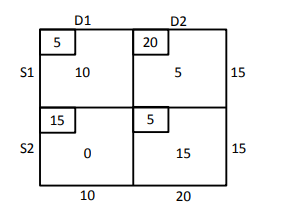
\includegraphics[width=0.75\columnwidth]{chapters/10/7/2/4/figs/fig.png}
 \end{center}
\caption{}
\label{fig:10/7/2/4Fig1}
\end{figure}
\fi

\item Find the position vector of the mid point of the vector joining the points $\vec{P}$(2, 3, 4)
and $\vec{Q}$(4, 1, –2).
\\
\solution
		\begin{enumerate}[label=\thesubsection.\arabic*,ref=\thesubsection.\theenumi]
\item Find the coordinates of the point which divides the join of $(-1,7) $ and $ (4,-3)$ in the ratio 2:3.
	\\
		\solution
	\begin{enumerate}[label=\thesubsection.\arabic*,ref=\thesubsection.\theenumi]
\item Find the coordinates of the point which divides the join of $(-1,7) $ and $ (4,-3)$ in the ratio 2:3.
	\\
		\solution
	\input{chapters/10/7/2/1/section.tex}
\item Find the coordinates of the point $\vec{R}$ on the line segment joining the points $\vec{P}(-1,3)$ and $\vec{Q}(2,5)$ such that $PR=\frac{3}{5}PQ$.
\item Find the ratio in which the point $\vec{P}\brak{\frac{3}{4},\frac{5}{12}}$ divides the line segment joining the points $\vec{A}\brak{\frac{1}{2},\frac{3}{2}}$ and $ \vec{B}(2,-5)$.
\item Find the coordinates of the point which divides the line segment joining the points $(4,-3)$ and $(8,5)$ in the ratio $3:1$ internally.
\item Find the coordinates of the point $\vec{P}$ on $AD$ such that $AP : PD = 2 : 1$.
\item If the point $\vec{P} (2, 1)$ lies on the line segment joining points $\vec{A} (4, 2)$  and $ \vec{B} (8, 4)$,
then
\begin{enumerate}
	\item $AP =\frac{1}{3}{AB}$ 
\item ${AP}={PE}$
\item ${PB}=\frac{1}{3}{AB}$
\item${AP}=\frac{1}{2}{AB}$
 \end{enumerate}
\item Find the ratio in which the line segment joining the points $(-3,10)$  and  $(6,-8)$  is divided by $ (-1,6)$.
	\\
		\solution
	\input{chapters/10/7/2/4/section.tex}
\item Find the position vector of the mid point of the vector joining the points $\vec{P}$(2, 3, 4)
and $\vec{Q}$(4, 1, –2).
\\
\solution
		\input{chapters/12/10/2/16/section.tex}
\item Let $\vec{A}(4, 2), \vec{B}(6, 5)$  and $ \vec{C}(1, 4)$ be the vertices of $\triangle ABC$.
\begin{enumerate}
\item If $\vec{A}$ and  $\vec{B}$ are $(-2,-2)$ and  $(2,-4)$, respectively, find the coordinates of $\vec{P}$ such that $AP= \frac {3}{7}AB$  and $ \vec{P}$ lies on the line segment $AB$.
	\\
		\solution
	\input{chapters/10/7/2/8/section.tex}
\item Find the coordinates of the points which divide the line segment joining $A(-2,2)$  and  $\vec{B}(2,8)$ into four equal parts.
	\\
		\solution
	\input{chapters/10/7/2/9/section.tex}
\item In what ratio does the point $(-4,6)$ divide the line segment joining the points $\vec{A}(-6,0)$ and $\vec{B}(3,-8)$?
\item Given that $\vec{P}(3,2,-4), \vec{Q}(5,4,-6)$ and $\vec{R}(9,8,-10)$ are collinear. Find the ratio in which $\vec{Q}$ divides $PR$.
\item Points $\vec{A}(-6,10),\vec{B}(-4,6)$  and  $\vec{C}(3,-8)$ are collinear such that $AB=  \frac{2}{9}AC$.
\item The point which divides the line segment joining the points $\vec{P} (7, –6) $  and  $\vec{Q}(3, 4)$ in the 
ratio 1 : 2 internally lies in  which quadrant?
\item Find the coordinates of the points of trisection of the line segment joining $(4,-1)$  and  $(-2,3)$.
	\\
		\solution
	\input{chapters/10/7/2/2/section.tex}
\item Find the coordinates of the points which trisect the line segment joining the points $\vec{P}(4,2,-6)$ and $\vec{Q}(10,-16,6)$.
\item Find the coordinates of the points of trisection (i.e. points dividing to three equal parts) of the line segment joining the points $\vec{A}(2,-2)$ and $\vec{B}(-7,4)$.
\item Point $\vec{P}(5,-3)$ is one of the two points of trisection of line segment joining the points $\vec{A}(7,-2)$ and $\vec{B}(1,-5)$
\item Find the position vector of a point $\vec{R}$ which divides the line joining two points $\vec{P}$
and $\vec{Q}$ whose position vectors are $\hat{i}+2\hat{j}-\hat{k}$ and $-\hat{i}+\hat{j}+\hat{k}$ respectively, in the
ratio 2 : 1
\begin{enumerate}
    \item  internally
    \item  externally
\end{enumerate}
%\solution
%		\input{chapters/12/10/2/15/section.tex}
\item Find the coordinates of the point which divides the line segment joining the points which divides the line segment joining  the points $(-2,3,5)$ and $(1,-4,6)$ in the ratio 
\begin{enumerate}
\item $2:3$ internally,
\item $2:3$ externally
\end{enumerate}
\item Find the coordinates of the point which divides the line segment joining the points $(1,-2,3)$ and $(3,4,-5)$ in the ratio $2:3$
\begin{enumerate}
\item internally, and
\item externally
\end{enumerate}
\item Consider two points $\vec{P}$ and $\vec{Q}$ with position vectors $\overrightarrow{OP} = 3\overrightarrow{a}-2\overrightarrow{b}$ and $\overrightarrow{OQ}=\overrightarrow{a}+\overrightarrow{b}$. Find the position vector of a point $\vec{R}$ which divides the line joining $\vec{P}$ and $\vec{Q}$ in the ratio $2:1$, 
\begin{enumerate}
\item internally, and 
\item externally.
\end{enumerate}
\item The median from $\vec{A}$ meets $BC$ at $\vec{D}$. Find the coordinates of the point $\vec{D}$.
\item Find the coordinates of points $\vec{Q}$ and $\vec{R}$ on medians $BE$ and $CF$ respectively such that $BQ : QE = 2 : 1$  and  $CR : RF = 2 : 1$.
\item What do you observe?
\item If $\vec{A}, \vec{B}$ and $\vec{C}$  are the vertices of $\triangle ABC$, find the coordinates of the centroid of the triangle.
\end{enumerate}
\solution
	\input{chapters/10/7/4/7/section.tex}
\item If $\vec{P}(9a-2,-b)$ divides line segment joining $\vec{A}(3a+1,-3)$ and $\vec{B}(8a,5)$ in the ratio 3:1, find the values of $a$ and $b$.
\item Find the position vector of a point $\vec{R}$ which divides the line joining two points $\vec{P}$ and $\vec{Q}$ whose position vectors are $2\vec{a}+\vec{b}$ and $\vec{a}-3\vec{b}$ externally in the ratio $1:2$.
\item The position vector of the point which divides the join of points 2$\vec{a}$-3$\vec{b}$ $\text{and}$ $\vec{a}+\vec{b}$ in the ratio 3:1 is \rule{1cm}{0.1pt}.
\item If $\vec{a}$ and $\vec{b}$ are the postion vectors of $\vec{A}$ and $\vec{B}$, respectively, find the position vector of a point $\vec{C}$ in $BA$ produced such that $BC=1.5BA$.
\item Find the position vector of a point $\vec{R}$ which divides the line joining two points $\vec{P}$ and $\vec{Q}$ whose position vectors are $(2\vec{a}+\vec{b})$ and $(\vec{a}-3\vec{b})$
externally in the ratio 1 : 2. Also, show that $\vec{P}$ is the mid point of the line segment $RQ$.
\end{enumerate}

\item Find the coordinates of the point $\vec{R}$ on the line segment joining the points $\vec{P}(-1,3)$ and $\vec{Q}(2,5)$ such that $PR=\frac{3}{5}PQ$.
\item Find the ratio in which the point $\vec{P}\brak{\frac{3}{4},\frac{5}{12}}$ divides the line segment joining the points $\vec{A}\brak{\frac{1}{2},\frac{3}{2}}$ and $ \vec{B}(2,-5)$.
\item Find the coordinates of the point which divides the line segment joining the points $(4,-3)$ and $(8,5)$ in the ratio $3:1$ internally.
\item Find the coordinates of the point $\vec{P}$ on $AD$ such that $AP : PD = 2 : 1$.
\item If the point $\vec{P} (2, 1)$ lies on the line segment joining points $\vec{A} (4, 2)$  and $ \vec{B} (8, 4)$,
then
\begin{enumerate}
	\item $AP =\frac{1}{3}{AB}$ 
\item ${AP}={PE}$
\item ${PB}=\frac{1}{3}{AB}$
\item${AP}=\frac{1}{2}{AB}$
 \end{enumerate}
\item Find the ratio in which the line segment joining the points $(-3,10)$  and  $(6,-8)$  is divided by $ (-1,6)$.
	\\
		\solution
	\iffalse
Using section formula,
\begin{align}
         \myvec{-1\\6} &=\frac{{\myvec{-3\\10}+k\myvec{6\\-8}}}{1+k}\\
	 \implies 7k\myvec{1 \\ -2} &= 2\myvec{1 \\ -2}
	 \\
	 \text{or, } k &= \frac{2}{7}.
\end{align}
\fi
In 
			\eqref{eq:section_formula-k}, substituting
			\begin{align}
				\vec{B} &= \myvec{-3\\10}, \vec{C} = \myvec{6\\-8}, \vec{D} = \myvec{-1\\6},
				\\
				k &= \frac{\myvec{-2 & 4}\myvec{-7 \\ 14}}{\norm{\myvec{-7 \\ 14}}^2} = \frac{2}{7}
			\end{align}
\iffalse
See \figref{fig:10/7/2/4Fig1}.
\begin{figure}[H]
 \begin{center}
  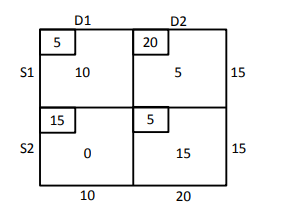
\includegraphics[width=0.75\columnwidth]{chapters/10/7/2/4/figs/fig.png}
 \end{center}
\caption{}
\label{fig:10/7/2/4Fig1}
\end{figure}
\fi

\item Find the position vector of the mid point of the vector joining the points $\vec{P}$(2, 3, 4)
and $\vec{Q}$(4, 1, –2).
\\
\solution
		\begin{enumerate}[label=\thesubsection.\arabic*,ref=\thesubsection.\theenumi]
\item Find the coordinates of the point which divides the join of $(-1,7) $ and $ (4,-3)$ in the ratio 2:3.
	\\
		\solution
	\input{chapters/10/7/2/1/section.tex}
\item Find the coordinates of the point $\vec{R}$ on the line segment joining the points $\vec{P}(-1,3)$ and $\vec{Q}(2,5)$ such that $PR=\frac{3}{5}PQ$.
\item Find the ratio in which the point $\vec{P}\brak{\frac{3}{4},\frac{5}{12}}$ divides the line segment joining the points $\vec{A}\brak{\frac{1}{2},\frac{3}{2}}$ and $ \vec{B}(2,-5)$.
\item Find the coordinates of the point which divides the line segment joining the points $(4,-3)$ and $(8,5)$ in the ratio $3:1$ internally.
\item Find the coordinates of the point $\vec{P}$ on $AD$ such that $AP : PD = 2 : 1$.
\item If the point $\vec{P} (2, 1)$ lies on the line segment joining points $\vec{A} (4, 2)$  and $ \vec{B} (8, 4)$,
then
\begin{enumerate}
	\item $AP =\frac{1}{3}{AB}$ 
\item ${AP}={PE}$
\item ${PB}=\frac{1}{3}{AB}$
\item${AP}=\frac{1}{2}{AB}$
 \end{enumerate}
\item Find the ratio in which the line segment joining the points $(-3,10)$  and  $(6,-8)$  is divided by $ (-1,6)$.
	\\
		\solution
	\input{chapters/10/7/2/4/section.tex}
\item Find the position vector of the mid point of the vector joining the points $\vec{P}$(2, 3, 4)
and $\vec{Q}$(4, 1, –2).
\\
\solution
		\input{chapters/12/10/2/16/section.tex}
\item Let $\vec{A}(4, 2), \vec{B}(6, 5)$  and $ \vec{C}(1, 4)$ be the vertices of $\triangle ABC$.
\begin{enumerate}
\item If $\vec{A}$ and  $\vec{B}$ are $(-2,-2)$ and  $(2,-4)$, respectively, find the coordinates of $\vec{P}$ such that $AP= \frac {3}{7}AB$  and $ \vec{P}$ lies on the line segment $AB$.
	\\
		\solution
	\input{chapters/10/7/2/8/section.tex}
\item Find the coordinates of the points which divide the line segment joining $A(-2,2)$  and  $\vec{B}(2,8)$ into four equal parts.
	\\
		\solution
	\input{chapters/10/7/2/9/section.tex}
\item In what ratio does the point $(-4,6)$ divide the line segment joining the points $\vec{A}(-6,0)$ and $\vec{B}(3,-8)$?
\item Given that $\vec{P}(3,2,-4), \vec{Q}(5,4,-6)$ and $\vec{R}(9,8,-10)$ are collinear. Find the ratio in which $\vec{Q}$ divides $PR$.
\item Points $\vec{A}(-6,10),\vec{B}(-4,6)$  and  $\vec{C}(3,-8)$ are collinear such that $AB=  \frac{2}{9}AC$.
\item The point which divides the line segment joining the points $\vec{P} (7, –6) $  and  $\vec{Q}(3, 4)$ in the 
ratio 1 : 2 internally lies in  which quadrant?
\item Find the coordinates of the points of trisection of the line segment joining $(4,-1)$  and  $(-2,3)$.
	\\
		\solution
	\input{chapters/10/7/2/2/section.tex}
\item Find the coordinates of the points which trisect the line segment joining the points $\vec{P}(4,2,-6)$ and $\vec{Q}(10,-16,6)$.
\item Find the coordinates of the points of trisection (i.e. points dividing to three equal parts) of the line segment joining the points $\vec{A}(2,-2)$ and $\vec{B}(-7,4)$.
\item Point $\vec{P}(5,-3)$ is one of the two points of trisection of line segment joining the points $\vec{A}(7,-2)$ and $\vec{B}(1,-5)$
\item Find the position vector of a point $\vec{R}$ which divides the line joining two points $\vec{P}$
and $\vec{Q}$ whose position vectors are $\hat{i}+2\hat{j}-\hat{k}$ and $-\hat{i}+\hat{j}+\hat{k}$ respectively, in the
ratio 2 : 1
\begin{enumerate}
    \item  internally
    \item  externally
\end{enumerate}
%\solution
%		\input{chapters/12/10/2/15/section.tex}
\item Find the coordinates of the point which divides the line segment joining the points which divides the line segment joining  the points $(-2,3,5)$ and $(1,-4,6)$ in the ratio 
\begin{enumerate}
\item $2:3$ internally,
\item $2:3$ externally
\end{enumerate}
\item Find the coordinates of the point which divides the line segment joining the points $(1,-2,3)$ and $(3,4,-5)$ in the ratio $2:3$
\begin{enumerate}
\item internally, and
\item externally
\end{enumerate}
\item Consider two points $\vec{P}$ and $\vec{Q}$ with position vectors $\overrightarrow{OP} = 3\overrightarrow{a}-2\overrightarrow{b}$ and $\overrightarrow{OQ}=\overrightarrow{a}+\overrightarrow{b}$. Find the position vector of a point $\vec{R}$ which divides the line joining $\vec{P}$ and $\vec{Q}$ in the ratio $2:1$, 
\begin{enumerate}
\item internally, and 
\item externally.
\end{enumerate}
\item The median from $\vec{A}$ meets $BC$ at $\vec{D}$. Find the coordinates of the point $\vec{D}$.
\item Find the coordinates of points $\vec{Q}$ and $\vec{R}$ on medians $BE$ and $CF$ respectively such that $BQ : QE = 2 : 1$  and  $CR : RF = 2 : 1$.
\item What do you observe?
\item If $\vec{A}, \vec{B}$ and $\vec{C}$  are the vertices of $\triangle ABC$, find the coordinates of the centroid of the triangle.
\end{enumerate}
\solution
	\input{chapters/10/7/4/7/section.tex}
\item If $\vec{P}(9a-2,-b)$ divides line segment joining $\vec{A}(3a+1,-3)$ and $\vec{B}(8a,5)$ in the ratio 3:1, find the values of $a$ and $b$.
\item Find the position vector of a point $\vec{R}$ which divides the line joining two points $\vec{P}$ and $\vec{Q}$ whose position vectors are $2\vec{a}+\vec{b}$ and $\vec{a}-3\vec{b}$ externally in the ratio $1:2$.
\item The position vector of the point which divides the join of points 2$\vec{a}$-3$\vec{b}$ $\text{and}$ $\vec{a}+\vec{b}$ in the ratio 3:1 is \rule{1cm}{0.1pt}.
\item If $\vec{a}$ and $\vec{b}$ are the postion vectors of $\vec{A}$ and $\vec{B}$, respectively, find the position vector of a point $\vec{C}$ in $BA$ produced such that $BC=1.5BA$.
\item Find the position vector of a point $\vec{R}$ which divides the line joining two points $\vec{P}$ and $\vec{Q}$ whose position vectors are $(2\vec{a}+\vec{b})$ and $(\vec{a}-3\vec{b})$
externally in the ratio 1 : 2. Also, show that $\vec{P}$ is the mid point of the line segment $RQ$.
\end{enumerate}

\item Let $\vec{A}(4, 2), \vec{B}(6, 5)$  and $ \vec{C}(1, 4)$ be the vertices of $\triangle ABC$.
\begin{enumerate}
\item If $\vec{A}$ and  $\vec{B}$ are $(-2,-2)$ and  $(2,-4)$, respectively, find the coordinates of $\vec{P}$ such that $AP= \frac {3}{7}AB$  and $ \vec{P}$ lies on the line segment $AB$.
	\\
		\solution
	\begin{enumerate}[label=\thesubsection.\arabic*,ref=\thesubsection.\theenumi]
\item Find the coordinates of the point which divides the join of $(-1,7) $ and $ (4,-3)$ in the ratio 2:3.
	\\
		\solution
	\input{chapters/10/7/2/1/section.tex}
\item Find the coordinates of the point $\vec{R}$ on the line segment joining the points $\vec{P}(-1,3)$ and $\vec{Q}(2,5)$ such that $PR=\frac{3}{5}PQ$.
\item Find the ratio in which the point $\vec{P}\brak{\frac{3}{4},\frac{5}{12}}$ divides the line segment joining the points $\vec{A}\brak{\frac{1}{2},\frac{3}{2}}$ and $ \vec{B}(2,-5)$.
\item Find the coordinates of the point which divides the line segment joining the points $(4,-3)$ and $(8,5)$ in the ratio $3:1$ internally.
\item Find the coordinates of the point $\vec{P}$ on $AD$ such that $AP : PD = 2 : 1$.
\item If the point $\vec{P} (2, 1)$ lies on the line segment joining points $\vec{A} (4, 2)$  and $ \vec{B} (8, 4)$,
then
\begin{enumerate}
	\item $AP =\frac{1}{3}{AB}$ 
\item ${AP}={PE}$
\item ${PB}=\frac{1}{3}{AB}$
\item${AP}=\frac{1}{2}{AB}$
 \end{enumerate}
\item Find the ratio in which the line segment joining the points $(-3,10)$  and  $(6,-8)$  is divided by $ (-1,6)$.
	\\
		\solution
	\input{chapters/10/7/2/4/section.tex}
\item Find the position vector of the mid point of the vector joining the points $\vec{P}$(2, 3, 4)
and $\vec{Q}$(4, 1, –2).
\\
\solution
		\input{chapters/12/10/2/16/section.tex}
\item Let $\vec{A}(4, 2), \vec{B}(6, 5)$  and $ \vec{C}(1, 4)$ be the vertices of $\triangle ABC$.
\begin{enumerate}
\item If $\vec{A}$ and  $\vec{B}$ are $(-2,-2)$ and  $(2,-4)$, respectively, find the coordinates of $\vec{P}$ such that $AP= \frac {3}{7}AB$  and $ \vec{P}$ lies on the line segment $AB$.
	\\
		\solution
	\input{chapters/10/7/2/8/section.tex}
\item Find the coordinates of the points which divide the line segment joining $A(-2,2)$  and  $\vec{B}(2,8)$ into four equal parts.
	\\
		\solution
	\input{chapters/10/7/2/9/section.tex}
\item In what ratio does the point $(-4,6)$ divide the line segment joining the points $\vec{A}(-6,0)$ and $\vec{B}(3,-8)$?
\item Given that $\vec{P}(3,2,-4), \vec{Q}(5,4,-6)$ and $\vec{R}(9,8,-10)$ are collinear. Find the ratio in which $\vec{Q}$ divides $PR$.
\item Points $\vec{A}(-6,10),\vec{B}(-4,6)$  and  $\vec{C}(3,-8)$ are collinear such that $AB=  \frac{2}{9}AC$.
\item The point which divides the line segment joining the points $\vec{P} (7, –6) $  and  $\vec{Q}(3, 4)$ in the 
ratio 1 : 2 internally lies in  which quadrant?
\item Find the coordinates of the points of trisection of the line segment joining $(4,-1)$  and  $(-2,3)$.
	\\
		\solution
	\input{chapters/10/7/2/2/section.tex}
\item Find the coordinates of the points which trisect the line segment joining the points $\vec{P}(4,2,-6)$ and $\vec{Q}(10,-16,6)$.
\item Find the coordinates of the points of trisection (i.e. points dividing to three equal parts) of the line segment joining the points $\vec{A}(2,-2)$ and $\vec{B}(-7,4)$.
\item Point $\vec{P}(5,-3)$ is one of the two points of trisection of line segment joining the points $\vec{A}(7,-2)$ and $\vec{B}(1,-5)$
\item Find the position vector of a point $\vec{R}$ which divides the line joining two points $\vec{P}$
and $\vec{Q}$ whose position vectors are $\hat{i}+2\hat{j}-\hat{k}$ and $-\hat{i}+\hat{j}+\hat{k}$ respectively, in the
ratio 2 : 1
\begin{enumerate}
    \item  internally
    \item  externally
\end{enumerate}
%\solution
%		\input{chapters/12/10/2/15/section.tex}
\item Find the coordinates of the point which divides the line segment joining the points which divides the line segment joining  the points $(-2,3,5)$ and $(1,-4,6)$ in the ratio 
\begin{enumerate}
\item $2:3$ internally,
\item $2:3$ externally
\end{enumerate}
\item Find the coordinates of the point which divides the line segment joining the points $(1,-2,3)$ and $(3,4,-5)$ in the ratio $2:3$
\begin{enumerate}
\item internally, and
\item externally
\end{enumerate}
\item Consider two points $\vec{P}$ and $\vec{Q}$ with position vectors $\overrightarrow{OP} = 3\overrightarrow{a}-2\overrightarrow{b}$ and $\overrightarrow{OQ}=\overrightarrow{a}+\overrightarrow{b}$. Find the position vector of a point $\vec{R}$ which divides the line joining $\vec{P}$ and $\vec{Q}$ in the ratio $2:1$, 
\begin{enumerate}
\item internally, and 
\item externally.
\end{enumerate}
\item The median from $\vec{A}$ meets $BC$ at $\vec{D}$. Find the coordinates of the point $\vec{D}$.
\item Find the coordinates of points $\vec{Q}$ and $\vec{R}$ on medians $BE$ and $CF$ respectively such that $BQ : QE = 2 : 1$  and  $CR : RF = 2 : 1$.
\item What do you observe?
\item If $\vec{A}, \vec{B}$ and $\vec{C}$  are the vertices of $\triangle ABC$, find the coordinates of the centroid of the triangle.
\end{enumerate}
\solution
	\input{chapters/10/7/4/7/section.tex}
\item If $\vec{P}(9a-2,-b)$ divides line segment joining $\vec{A}(3a+1,-3)$ and $\vec{B}(8a,5)$ in the ratio 3:1, find the values of $a$ and $b$.
\item Find the position vector of a point $\vec{R}$ which divides the line joining two points $\vec{P}$ and $\vec{Q}$ whose position vectors are $2\vec{a}+\vec{b}$ and $\vec{a}-3\vec{b}$ externally in the ratio $1:2$.
\item The position vector of the point which divides the join of points 2$\vec{a}$-3$\vec{b}$ $\text{and}$ $\vec{a}+\vec{b}$ in the ratio 3:1 is \rule{1cm}{0.1pt}.
\item If $\vec{a}$ and $\vec{b}$ are the postion vectors of $\vec{A}$ and $\vec{B}$, respectively, find the position vector of a point $\vec{C}$ in $BA$ produced such that $BC=1.5BA$.
\item Find the position vector of a point $\vec{R}$ which divides the line joining two points $\vec{P}$ and $\vec{Q}$ whose position vectors are $(2\vec{a}+\vec{b})$ and $(\vec{a}-3\vec{b})$
externally in the ratio 1 : 2. Also, show that $\vec{P}$ is the mid point of the line segment $RQ$.
\end{enumerate}

\item Find the coordinates of the points which divide the line segment joining $A(-2,2)$  and  $\vec{B}(2,8)$ into four equal parts.
	\\
		\solution
	\begin{enumerate}[label=\thesubsection.\arabic*,ref=\thesubsection.\theenumi]
\item Find the coordinates of the point which divides the join of $(-1,7) $ and $ (4,-3)$ in the ratio 2:3.
	\\
		\solution
	\input{chapters/10/7/2/1/section.tex}
\item Find the coordinates of the point $\vec{R}$ on the line segment joining the points $\vec{P}(-1,3)$ and $\vec{Q}(2,5)$ such that $PR=\frac{3}{5}PQ$.
\item Find the ratio in which the point $\vec{P}\brak{\frac{3}{4},\frac{5}{12}}$ divides the line segment joining the points $\vec{A}\brak{\frac{1}{2},\frac{3}{2}}$ and $ \vec{B}(2,-5)$.
\item Find the coordinates of the point which divides the line segment joining the points $(4,-3)$ and $(8,5)$ in the ratio $3:1$ internally.
\item Find the coordinates of the point $\vec{P}$ on $AD$ such that $AP : PD = 2 : 1$.
\item If the point $\vec{P} (2, 1)$ lies on the line segment joining points $\vec{A} (4, 2)$  and $ \vec{B} (8, 4)$,
then
\begin{enumerate}
	\item $AP =\frac{1}{3}{AB}$ 
\item ${AP}={PE}$
\item ${PB}=\frac{1}{3}{AB}$
\item${AP}=\frac{1}{2}{AB}$
 \end{enumerate}
\item Find the ratio in which the line segment joining the points $(-3,10)$  and  $(6,-8)$  is divided by $ (-1,6)$.
	\\
		\solution
	\input{chapters/10/7/2/4/section.tex}
\item Find the position vector of the mid point of the vector joining the points $\vec{P}$(2, 3, 4)
and $\vec{Q}$(4, 1, –2).
\\
\solution
		\input{chapters/12/10/2/16/section.tex}
\item Let $\vec{A}(4, 2), \vec{B}(6, 5)$  and $ \vec{C}(1, 4)$ be the vertices of $\triangle ABC$.
\begin{enumerate}
\item If $\vec{A}$ and  $\vec{B}$ are $(-2,-2)$ and  $(2,-4)$, respectively, find the coordinates of $\vec{P}$ such that $AP= \frac {3}{7}AB$  and $ \vec{P}$ lies on the line segment $AB$.
	\\
		\solution
	\input{chapters/10/7/2/8/section.tex}
\item Find the coordinates of the points which divide the line segment joining $A(-2,2)$  and  $\vec{B}(2,8)$ into four equal parts.
	\\
		\solution
	\input{chapters/10/7/2/9/section.tex}
\item In what ratio does the point $(-4,6)$ divide the line segment joining the points $\vec{A}(-6,0)$ and $\vec{B}(3,-8)$?
\item Given that $\vec{P}(3,2,-4), \vec{Q}(5,4,-6)$ and $\vec{R}(9,8,-10)$ are collinear. Find the ratio in which $\vec{Q}$ divides $PR$.
\item Points $\vec{A}(-6,10),\vec{B}(-4,6)$  and  $\vec{C}(3,-8)$ are collinear such that $AB=  \frac{2}{9}AC$.
\item The point which divides the line segment joining the points $\vec{P} (7, –6) $  and  $\vec{Q}(3, 4)$ in the 
ratio 1 : 2 internally lies in  which quadrant?
\item Find the coordinates of the points of trisection of the line segment joining $(4,-1)$  and  $(-2,3)$.
	\\
		\solution
	\input{chapters/10/7/2/2/section.tex}
\item Find the coordinates of the points which trisect the line segment joining the points $\vec{P}(4,2,-6)$ and $\vec{Q}(10,-16,6)$.
\item Find the coordinates of the points of trisection (i.e. points dividing to three equal parts) of the line segment joining the points $\vec{A}(2,-2)$ and $\vec{B}(-7,4)$.
\item Point $\vec{P}(5,-3)$ is one of the two points of trisection of line segment joining the points $\vec{A}(7,-2)$ and $\vec{B}(1,-5)$
\item Find the position vector of a point $\vec{R}$ which divides the line joining two points $\vec{P}$
and $\vec{Q}$ whose position vectors are $\hat{i}+2\hat{j}-\hat{k}$ and $-\hat{i}+\hat{j}+\hat{k}$ respectively, in the
ratio 2 : 1
\begin{enumerate}
    \item  internally
    \item  externally
\end{enumerate}
%\solution
%		\input{chapters/12/10/2/15/section.tex}
\item Find the coordinates of the point which divides the line segment joining the points which divides the line segment joining  the points $(-2,3,5)$ and $(1,-4,6)$ in the ratio 
\begin{enumerate}
\item $2:3$ internally,
\item $2:3$ externally
\end{enumerate}
\item Find the coordinates of the point which divides the line segment joining the points $(1,-2,3)$ and $(3,4,-5)$ in the ratio $2:3$
\begin{enumerate}
\item internally, and
\item externally
\end{enumerate}
\item Consider two points $\vec{P}$ and $\vec{Q}$ with position vectors $\overrightarrow{OP} = 3\overrightarrow{a}-2\overrightarrow{b}$ and $\overrightarrow{OQ}=\overrightarrow{a}+\overrightarrow{b}$. Find the position vector of a point $\vec{R}$ which divides the line joining $\vec{P}$ and $\vec{Q}$ in the ratio $2:1$, 
\begin{enumerate}
\item internally, and 
\item externally.
\end{enumerate}
\item The median from $\vec{A}$ meets $BC$ at $\vec{D}$. Find the coordinates of the point $\vec{D}$.
\item Find the coordinates of points $\vec{Q}$ and $\vec{R}$ on medians $BE$ and $CF$ respectively such that $BQ : QE = 2 : 1$  and  $CR : RF = 2 : 1$.
\item What do you observe?
\item If $\vec{A}, \vec{B}$ and $\vec{C}$  are the vertices of $\triangle ABC$, find the coordinates of the centroid of the triangle.
\end{enumerate}
\solution
	\input{chapters/10/7/4/7/section.tex}
\item If $\vec{P}(9a-2,-b)$ divides line segment joining $\vec{A}(3a+1,-3)$ and $\vec{B}(8a,5)$ in the ratio 3:1, find the values of $a$ and $b$.
\item Find the position vector of a point $\vec{R}$ which divides the line joining two points $\vec{P}$ and $\vec{Q}$ whose position vectors are $2\vec{a}+\vec{b}$ and $\vec{a}-3\vec{b}$ externally in the ratio $1:2$.
\item The position vector of the point which divides the join of points 2$\vec{a}$-3$\vec{b}$ $\text{and}$ $\vec{a}+\vec{b}$ in the ratio 3:1 is \rule{1cm}{0.1pt}.
\item If $\vec{a}$ and $\vec{b}$ are the postion vectors of $\vec{A}$ and $\vec{B}$, respectively, find the position vector of a point $\vec{C}$ in $BA$ produced such that $BC=1.5BA$.
\item Find the position vector of a point $\vec{R}$ which divides the line joining two points $\vec{P}$ and $\vec{Q}$ whose position vectors are $(2\vec{a}+\vec{b})$ and $(\vec{a}-3\vec{b})$
externally in the ratio 1 : 2. Also, show that $\vec{P}$ is the mid point of the line segment $RQ$.
\end{enumerate}

\item In what ratio does the point $(-4,6)$ divide the line segment joining the points $\vec{A}(-6,0)$ and $\vec{B}(3,-8)$?
\item Given that $\vec{P}(3,2,-4), \vec{Q}(5,4,-6)$ and $\vec{R}(9,8,-10)$ are collinear. Find the ratio in which $\vec{Q}$ divides $PR$.
\item Points $\vec{A}(-6,10),\vec{B}(-4,6)$  and  $\vec{C}(3,-8)$ are collinear such that $AB=  \frac{2}{9}AC$.
\item The point which divides the line segment joining the points $\vec{P} (7, –6) $  and  $\vec{Q}(3, 4)$ in the 
ratio 1 : 2 internally lies in  which quadrant?
\item Find the coordinates of the points of trisection of the line segment joining $(4,-1)$  and  $(-2,3)$.
	\\
		\solution
	Using section formula,
\begin{align}
\vec{R}=\frac{1}{1+\frac{1}{2}}\brak{\myvec{4\\-1}+\frac{1}{2}\myvec{-2\\3}}
=\myvec{2\\ \frac{1}{3}}\\
\vec{S}=\frac{1}{1+\frac{2}{1}}\brak{\myvec{4\\-1}+\frac{2}{1}\myvec{-2\\3}}
=\myvec{0\\ \frac{5}{3}}
\end{align}
which are the desired points of trisection.
\iffalse
See
		\figref{fig:chapters/10/7/2/2/Figure}
\begin{figure}[H]
\centering
\includegraphics[width=0.75\columnwidth]{chapters/10/7/2/2/figs/dj.pdf}
\caption{}
		\label{fig:chapters/10/7/2/2/Figure}
\end{figure}
\fi

\item Find the coordinates of the points which trisect the line segment joining the points $\vec{P}(4,2,-6)$ and $\vec{Q}(10,-16,6)$.
\item Find the coordinates of the points of trisection (i.e. points dividing to three equal parts) of the line segment joining the points $\vec{A}(2,-2)$ and $\vec{B}(-7,4)$.
\item Point $\vec{P}(5,-3)$ is one of the two points of trisection of line segment joining the points $\vec{A}(7,-2)$ and $\vec{B}(1,-5)$
\item Find the position vector of a point $\vec{R}$ which divides the line joining two points $\vec{P}$
and $\vec{Q}$ whose position vectors are $\hat{i}+2\hat{j}-\hat{k}$ and $-\hat{i}+\hat{j}+\hat{k}$ respectively, in the
ratio 2 : 1
\begin{enumerate}
    \item  internally
    \item  externally
\end{enumerate}
%\solution
%		\begin{enumerate}[label=\thesubsection.\arabic*,ref=\thesubsection.\theenumi]
\item Find the coordinates of the point which divides the join of $(-1,7) $ and $ (4,-3)$ in the ratio 2:3.
	\\
		\solution
	\input{chapters/10/7/2/1/section.tex}
\item Find the coordinates of the point $\vec{R}$ on the line segment joining the points $\vec{P}(-1,3)$ and $\vec{Q}(2,5)$ such that $PR=\frac{3}{5}PQ$.
\item Find the ratio in which the point $\vec{P}\brak{\frac{3}{4},\frac{5}{12}}$ divides the line segment joining the points $\vec{A}\brak{\frac{1}{2},\frac{3}{2}}$ and $ \vec{B}(2,-5)$.
\item Find the coordinates of the point which divides the line segment joining the points $(4,-3)$ and $(8,5)$ in the ratio $3:1$ internally.
\item Find the coordinates of the point $\vec{P}$ on $AD$ such that $AP : PD = 2 : 1$.
\item If the point $\vec{P} (2, 1)$ lies on the line segment joining points $\vec{A} (4, 2)$  and $ \vec{B} (8, 4)$,
then
\begin{enumerate}
	\item $AP =\frac{1}{3}{AB}$ 
\item ${AP}={PE}$
\item ${PB}=\frac{1}{3}{AB}$
\item${AP}=\frac{1}{2}{AB}$
 \end{enumerate}
\item Find the ratio in which the line segment joining the points $(-3,10)$  and  $(6,-8)$  is divided by $ (-1,6)$.
	\\
		\solution
	\input{chapters/10/7/2/4/section.tex}
\item Find the position vector of the mid point of the vector joining the points $\vec{P}$(2, 3, 4)
and $\vec{Q}$(4, 1, –2).
\\
\solution
		\input{chapters/12/10/2/16/section.tex}
\item Let $\vec{A}(4, 2), \vec{B}(6, 5)$  and $ \vec{C}(1, 4)$ be the vertices of $\triangle ABC$.
\begin{enumerate}
\item If $\vec{A}$ and  $\vec{B}$ are $(-2,-2)$ and  $(2,-4)$, respectively, find the coordinates of $\vec{P}$ such that $AP= \frac {3}{7}AB$  and $ \vec{P}$ lies on the line segment $AB$.
	\\
		\solution
	\input{chapters/10/7/2/8/section.tex}
\item Find the coordinates of the points which divide the line segment joining $A(-2,2)$  and  $\vec{B}(2,8)$ into four equal parts.
	\\
		\solution
	\input{chapters/10/7/2/9/section.tex}
\item In what ratio does the point $(-4,6)$ divide the line segment joining the points $\vec{A}(-6,0)$ and $\vec{B}(3,-8)$?
\item Given that $\vec{P}(3,2,-4), \vec{Q}(5,4,-6)$ and $\vec{R}(9,8,-10)$ are collinear. Find the ratio in which $\vec{Q}$ divides $PR$.
\item Points $\vec{A}(-6,10),\vec{B}(-4,6)$  and  $\vec{C}(3,-8)$ are collinear such that $AB=  \frac{2}{9}AC$.
\item The point which divides the line segment joining the points $\vec{P} (7, –6) $  and  $\vec{Q}(3, 4)$ in the 
ratio 1 : 2 internally lies in  which quadrant?
\item Find the coordinates of the points of trisection of the line segment joining $(4,-1)$  and  $(-2,3)$.
	\\
		\solution
	\input{chapters/10/7/2/2/section.tex}
\item Find the coordinates of the points which trisect the line segment joining the points $\vec{P}(4,2,-6)$ and $\vec{Q}(10,-16,6)$.
\item Find the coordinates of the points of trisection (i.e. points dividing to three equal parts) of the line segment joining the points $\vec{A}(2,-2)$ and $\vec{B}(-7,4)$.
\item Point $\vec{P}(5,-3)$ is one of the two points of trisection of line segment joining the points $\vec{A}(7,-2)$ and $\vec{B}(1,-5)$
\item Find the position vector of a point $\vec{R}$ which divides the line joining two points $\vec{P}$
and $\vec{Q}$ whose position vectors are $\hat{i}+2\hat{j}-\hat{k}$ and $-\hat{i}+\hat{j}+\hat{k}$ respectively, in the
ratio 2 : 1
\begin{enumerate}
    \item  internally
    \item  externally
\end{enumerate}
%\solution
%		\input{chapters/12/10/2/15/section.tex}
\item Find the coordinates of the point which divides the line segment joining the points which divides the line segment joining  the points $(-2,3,5)$ and $(1,-4,6)$ in the ratio 
\begin{enumerate}
\item $2:3$ internally,
\item $2:3$ externally
\end{enumerate}
\item Find the coordinates of the point which divides the line segment joining the points $(1,-2,3)$ and $(3,4,-5)$ in the ratio $2:3$
\begin{enumerate}
\item internally, and
\item externally
\end{enumerate}
\item Consider two points $\vec{P}$ and $\vec{Q}$ with position vectors $\overrightarrow{OP} = 3\overrightarrow{a}-2\overrightarrow{b}$ and $\overrightarrow{OQ}=\overrightarrow{a}+\overrightarrow{b}$. Find the position vector of a point $\vec{R}$ which divides the line joining $\vec{P}$ and $\vec{Q}$ in the ratio $2:1$, 
\begin{enumerate}
\item internally, and 
\item externally.
\end{enumerate}
\item The median from $\vec{A}$ meets $BC$ at $\vec{D}$. Find the coordinates of the point $\vec{D}$.
\item Find the coordinates of points $\vec{Q}$ and $\vec{R}$ on medians $BE$ and $CF$ respectively such that $BQ : QE = 2 : 1$  and  $CR : RF = 2 : 1$.
\item What do you observe?
\item If $\vec{A}, \vec{B}$ and $\vec{C}$  are the vertices of $\triangle ABC$, find the coordinates of the centroid of the triangle.
\end{enumerate}
\solution
	\input{chapters/10/7/4/7/section.tex}
\item If $\vec{P}(9a-2,-b)$ divides line segment joining $\vec{A}(3a+1,-3)$ and $\vec{B}(8a,5)$ in the ratio 3:1, find the values of $a$ and $b$.
\item Find the position vector of a point $\vec{R}$ which divides the line joining two points $\vec{P}$ and $\vec{Q}$ whose position vectors are $2\vec{a}+\vec{b}$ and $\vec{a}-3\vec{b}$ externally in the ratio $1:2$.
\item The position vector of the point which divides the join of points 2$\vec{a}$-3$\vec{b}$ $\text{and}$ $\vec{a}+\vec{b}$ in the ratio 3:1 is \rule{1cm}{0.1pt}.
\item If $\vec{a}$ and $\vec{b}$ are the postion vectors of $\vec{A}$ and $\vec{B}$, respectively, find the position vector of a point $\vec{C}$ in $BA$ produced such that $BC=1.5BA$.
\item Find the position vector of a point $\vec{R}$ which divides the line joining two points $\vec{P}$ and $\vec{Q}$ whose position vectors are $(2\vec{a}+\vec{b})$ and $(\vec{a}-3\vec{b})$
externally in the ratio 1 : 2. Also, show that $\vec{P}$ is the mid point of the line segment $RQ$.
\end{enumerate}

\item Find the coordinates of the point which divides the line segment joining the points which divides the line segment joining  the points $(-2,3,5)$ and $(1,-4,6)$ in the ratio 
\begin{enumerate}
\item $2:3$ internally,
\item $2:3$ externally
\end{enumerate}
\item Find the coordinates of the point which divides the line segment joining the points $(1,-2,3)$ and $(3,4,-5)$ in the ratio $2:3$
\begin{enumerate}
\item internally, and
\item externally
\end{enumerate}
\item Consider two points $\vec{P}$ and $\vec{Q}$ with position vectors $\overrightarrow{OP} = 3\overrightarrow{a}-2\overrightarrow{b}$ and $\overrightarrow{OQ}=\overrightarrow{a}+\overrightarrow{b}$. Find the position vector of a point $\vec{R}$ which divides the line joining $\vec{P}$ and $\vec{Q}$ in the ratio $2:1$, 
\begin{enumerate}
\item internally, and 
\item externally.
\end{enumerate}
\item The median from $\vec{A}$ meets $BC$ at $\vec{D}$. Find the coordinates of the point $\vec{D}$.
\item Find the coordinates of points $\vec{Q}$ and $\vec{R}$ on medians $BE$ and $CF$ respectively such that $BQ : QE = 2 : 1$  and  $CR : RF = 2 : 1$.
\item What do you observe?
\item If $\vec{A}, \vec{B}$ and $\vec{C}$  are the vertices of $\triangle ABC$, find the coordinates of the centroid of the triangle.
\end{enumerate}
\solution
	\begin{enumerate}[label=\thesubsection.\arabic*,ref=\thesubsection.\theenumi]
\item Find the coordinates of the point which divides the join of $(-1,7) $ and $ (4,-3)$ in the ratio 2:3.
	\\
		\solution
	\input{chapters/10/7/2/1/section.tex}
\item Find the coordinates of the point $\vec{R}$ on the line segment joining the points $\vec{P}(-1,3)$ and $\vec{Q}(2,5)$ such that $PR=\frac{3}{5}PQ$.
\item Find the ratio in which the point $\vec{P}\brak{\frac{3}{4},\frac{5}{12}}$ divides the line segment joining the points $\vec{A}\brak{\frac{1}{2},\frac{3}{2}}$ and $ \vec{B}(2,-5)$.
\item Find the coordinates of the point which divides the line segment joining the points $(4,-3)$ and $(8,5)$ in the ratio $3:1$ internally.
\item Find the coordinates of the point $\vec{P}$ on $AD$ such that $AP : PD = 2 : 1$.
\item If the point $\vec{P} (2, 1)$ lies on the line segment joining points $\vec{A} (4, 2)$  and $ \vec{B} (8, 4)$,
then
\begin{enumerate}
	\item $AP =\frac{1}{3}{AB}$ 
\item ${AP}={PE}$
\item ${PB}=\frac{1}{3}{AB}$
\item${AP}=\frac{1}{2}{AB}$
 \end{enumerate}
\item Find the ratio in which the line segment joining the points $(-3,10)$  and  $(6,-8)$  is divided by $ (-1,6)$.
	\\
		\solution
	\input{chapters/10/7/2/4/section.tex}
\item Find the position vector of the mid point of the vector joining the points $\vec{P}$(2, 3, 4)
and $\vec{Q}$(4, 1, –2).
\\
\solution
		\input{chapters/12/10/2/16/section.tex}
\item Let $\vec{A}(4, 2), \vec{B}(6, 5)$  and $ \vec{C}(1, 4)$ be the vertices of $\triangle ABC$.
\begin{enumerate}
\item If $\vec{A}$ and  $\vec{B}$ are $(-2,-2)$ and  $(2,-4)$, respectively, find the coordinates of $\vec{P}$ such that $AP= \frac {3}{7}AB$  and $ \vec{P}$ lies on the line segment $AB$.
	\\
		\solution
	\input{chapters/10/7/2/8/section.tex}
\item Find the coordinates of the points which divide the line segment joining $A(-2,2)$  and  $\vec{B}(2,8)$ into four equal parts.
	\\
		\solution
	\input{chapters/10/7/2/9/section.tex}
\item In what ratio does the point $(-4,6)$ divide the line segment joining the points $\vec{A}(-6,0)$ and $\vec{B}(3,-8)$?
\item Given that $\vec{P}(3,2,-4), \vec{Q}(5,4,-6)$ and $\vec{R}(9,8,-10)$ are collinear. Find the ratio in which $\vec{Q}$ divides $PR$.
\item Points $\vec{A}(-6,10),\vec{B}(-4,6)$  and  $\vec{C}(3,-8)$ are collinear such that $AB=  \frac{2}{9}AC$.
\item The point which divides the line segment joining the points $\vec{P} (7, –6) $  and  $\vec{Q}(3, 4)$ in the 
ratio 1 : 2 internally lies in  which quadrant?
\item Find the coordinates of the points of trisection of the line segment joining $(4,-1)$  and  $(-2,3)$.
	\\
		\solution
	\input{chapters/10/7/2/2/section.tex}
\item Find the coordinates of the points which trisect the line segment joining the points $\vec{P}(4,2,-6)$ and $\vec{Q}(10,-16,6)$.
\item Find the coordinates of the points of trisection (i.e. points dividing to three equal parts) of the line segment joining the points $\vec{A}(2,-2)$ and $\vec{B}(-7,4)$.
\item Point $\vec{P}(5,-3)$ is one of the two points of trisection of line segment joining the points $\vec{A}(7,-2)$ and $\vec{B}(1,-5)$
\item Find the position vector of a point $\vec{R}$ which divides the line joining two points $\vec{P}$
and $\vec{Q}$ whose position vectors are $\hat{i}+2\hat{j}-\hat{k}$ and $-\hat{i}+\hat{j}+\hat{k}$ respectively, in the
ratio 2 : 1
\begin{enumerate}
    \item  internally
    \item  externally
\end{enumerate}
%\solution
%		\input{chapters/12/10/2/15/section.tex}
\item Find the coordinates of the point which divides the line segment joining the points which divides the line segment joining  the points $(-2,3,5)$ and $(1,-4,6)$ in the ratio 
\begin{enumerate}
\item $2:3$ internally,
\item $2:3$ externally
\end{enumerate}
\item Find the coordinates of the point which divides the line segment joining the points $(1,-2,3)$ and $(3,4,-5)$ in the ratio $2:3$
\begin{enumerate}
\item internally, and
\item externally
\end{enumerate}
\item Consider two points $\vec{P}$ and $\vec{Q}$ with position vectors $\overrightarrow{OP} = 3\overrightarrow{a}-2\overrightarrow{b}$ and $\overrightarrow{OQ}=\overrightarrow{a}+\overrightarrow{b}$. Find the position vector of a point $\vec{R}$ which divides the line joining $\vec{P}$ and $\vec{Q}$ in the ratio $2:1$, 
\begin{enumerate}
\item internally, and 
\item externally.
\end{enumerate}
\item The median from $\vec{A}$ meets $BC$ at $\vec{D}$. Find the coordinates of the point $\vec{D}$.
\item Find the coordinates of points $\vec{Q}$ and $\vec{R}$ on medians $BE$ and $CF$ respectively such that $BQ : QE = 2 : 1$  and  $CR : RF = 2 : 1$.
\item What do you observe?
\item If $\vec{A}, \vec{B}$ and $\vec{C}$  are the vertices of $\triangle ABC$, find the coordinates of the centroid of the triangle.
\end{enumerate}
\solution
	\input{chapters/10/7/4/7/section.tex}
\item If $\vec{P}(9a-2,-b)$ divides line segment joining $\vec{A}(3a+1,-3)$ and $\vec{B}(8a,5)$ in the ratio 3:1, find the values of $a$ and $b$.
\item Find the position vector of a point $\vec{R}$ which divides the line joining two points $\vec{P}$ and $\vec{Q}$ whose position vectors are $2\vec{a}+\vec{b}$ and $\vec{a}-3\vec{b}$ externally in the ratio $1:2$.
\item The position vector of the point which divides the join of points 2$\vec{a}$-3$\vec{b}$ $\text{and}$ $\vec{a}+\vec{b}$ in the ratio 3:1 is \rule{1cm}{0.1pt}.
\item If $\vec{a}$ and $\vec{b}$ are the postion vectors of $\vec{A}$ and $\vec{B}$, respectively, find the position vector of a point $\vec{C}$ in $BA$ produced such that $BC=1.5BA$.
\item Find the position vector of a point $\vec{R}$ which divides the line joining two points $\vec{P}$ and $\vec{Q}$ whose position vectors are $(2\vec{a}+\vec{b})$ and $(\vec{a}-3\vec{b})$
externally in the ratio 1 : 2. Also, show that $\vec{P}$ is the mid point of the line segment $RQ$.
\end{enumerate}

\item If $\vec{P}(9a-2,-b)$ divides line segment joining $\vec{A}(3a+1,-3)$ and $\vec{B}(8a,5)$ in the ratio 3:1, find the values of $a$ and $b$.
\item Find the position vector of a point $\vec{R}$ which divides the line joining two points $\vec{P}$ and $\vec{Q}$ whose position vectors are $2\vec{a}+\vec{b}$ and $\vec{a}-3\vec{b}$ externally in the ratio $1:2$.
\item The position vector of the point which divides the join of points 2$\vec{a}$-3$\vec{b}$ $\text{and}$ $\vec{a}+\vec{b}$ in the ratio 3:1 is \rule{1cm}{0.1pt}.
\item If $\vec{a}$ and $\vec{b}$ are the postion vectors of $\vec{A}$ and $\vec{B}$, respectively, find the position vector of a point $\vec{C}$ in $BA$ produced such that $BC=1.5BA$.
\item Find the position vector of a point $\vec{R}$ which divides the line joining two points $\vec{P}$ and $\vec{Q}$ whose position vectors are $(2\vec{a}+\vec{b})$ and $(\vec{a}-3\vec{b})$
externally in the ratio 1 : 2. Also, show that $\vec{P}$ is the mid point of the line segment $RQ$.
\end{enumerate}

\item Let $\vec{A}(4, 2), \vec{B}(6, 5)$  and $ \vec{C}(1, 4)$ be the vertices of $\triangle ABC$.
\begin{enumerate}
\item If $\vec{A}$ and  $\vec{B}$ are $(-2,-2)$ and  $(2,-4)$, respectively, find the coordinates of $\vec{P}$ such that $AP= \frac {3}{7}AB$  and $ \vec{P}$ lies on the line segment $AB$.
	\\
		\solution
	\begin{enumerate}[label=\thesubsection.\arabic*,ref=\thesubsection.\theenumi]
\item Find the coordinates of the point which divides the join of $(-1,7) $ and $ (4,-3)$ in the ratio 2:3.
	\\
		\solution
	\begin{enumerate}[label=\thesubsection.\arabic*,ref=\thesubsection.\theenumi]
\item Find the coordinates of the point which divides the join of $(-1,7) $ and $ (4,-3)$ in the ratio 2:3.
	\\
		\solution
	\input{chapters/10/7/2/1/section.tex}
\item Find the coordinates of the point $\vec{R}$ on the line segment joining the points $\vec{P}(-1,3)$ and $\vec{Q}(2,5)$ such that $PR=\frac{3}{5}PQ$.
\item Find the ratio in which the point $\vec{P}\brak{\frac{3}{4},\frac{5}{12}}$ divides the line segment joining the points $\vec{A}\brak{\frac{1}{2},\frac{3}{2}}$ and $ \vec{B}(2,-5)$.
\item Find the coordinates of the point which divides the line segment joining the points $(4,-3)$ and $(8,5)$ in the ratio $3:1$ internally.
\item Find the coordinates of the point $\vec{P}$ on $AD$ such that $AP : PD = 2 : 1$.
\item If the point $\vec{P} (2, 1)$ lies on the line segment joining points $\vec{A} (4, 2)$  and $ \vec{B} (8, 4)$,
then
\begin{enumerate}
	\item $AP =\frac{1}{3}{AB}$ 
\item ${AP}={PE}$
\item ${PB}=\frac{1}{3}{AB}$
\item${AP}=\frac{1}{2}{AB}$
 \end{enumerate}
\item Find the ratio in which the line segment joining the points $(-3,10)$  and  $(6,-8)$  is divided by $ (-1,6)$.
	\\
		\solution
	\input{chapters/10/7/2/4/section.tex}
\item Find the position vector of the mid point of the vector joining the points $\vec{P}$(2, 3, 4)
and $\vec{Q}$(4, 1, –2).
\\
\solution
		\input{chapters/12/10/2/16/section.tex}
\item Let $\vec{A}(4, 2), \vec{B}(6, 5)$  and $ \vec{C}(1, 4)$ be the vertices of $\triangle ABC$.
\begin{enumerate}
\item If $\vec{A}$ and  $\vec{B}$ are $(-2,-2)$ and  $(2,-4)$, respectively, find the coordinates of $\vec{P}$ such that $AP= \frac {3}{7}AB$  and $ \vec{P}$ lies on the line segment $AB$.
	\\
		\solution
	\input{chapters/10/7/2/8/section.tex}
\item Find the coordinates of the points which divide the line segment joining $A(-2,2)$  and  $\vec{B}(2,8)$ into four equal parts.
	\\
		\solution
	\input{chapters/10/7/2/9/section.tex}
\item In what ratio does the point $(-4,6)$ divide the line segment joining the points $\vec{A}(-6,0)$ and $\vec{B}(3,-8)$?
\item Given that $\vec{P}(3,2,-4), \vec{Q}(5,4,-6)$ and $\vec{R}(9,8,-10)$ are collinear. Find the ratio in which $\vec{Q}$ divides $PR$.
\item Points $\vec{A}(-6,10),\vec{B}(-4,6)$  and  $\vec{C}(3,-8)$ are collinear such that $AB=  \frac{2}{9}AC$.
\item The point which divides the line segment joining the points $\vec{P} (7, –6) $  and  $\vec{Q}(3, 4)$ in the 
ratio 1 : 2 internally lies in  which quadrant?
\item Find the coordinates of the points of trisection of the line segment joining $(4,-1)$  and  $(-2,3)$.
	\\
		\solution
	\input{chapters/10/7/2/2/section.tex}
\item Find the coordinates of the points which trisect the line segment joining the points $\vec{P}(4,2,-6)$ and $\vec{Q}(10,-16,6)$.
\item Find the coordinates of the points of trisection (i.e. points dividing to three equal parts) of the line segment joining the points $\vec{A}(2,-2)$ and $\vec{B}(-7,4)$.
\item Point $\vec{P}(5,-3)$ is one of the two points of trisection of line segment joining the points $\vec{A}(7,-2)$ and $\vec{B}(1,-5)$
\item Find the position vector of a point $\vec{R}$ which divides the line joining two points $\vec{P}$
and $\vec{Q}$ whose position vectors are $\hat{i}+2\hat{j}-\hat{k}$ and $-\hat{i}+\hat{j}+\hat{k}$ respectively, in the
ratio 2 : 1
\begin{enumerate}
    \item  internally
    \item  externally
\end{enumerate}
%\solution
%		\input{chapters/12/10/2/15/section.tex}
\item Find the coordinates of the point which divides the line segment joining the points which divides the line segment joining  the points $(-2,3,5)$ and $(1,-4,6)$ in the ratio 
\begin{enumerate}
\item $2:3$ internally,
\item $2:3$ externally
\end{enumerate}
\item Find the coordinates of the point which divides the line segment joining the points $(1,-2,3)$ and $(3,4,-5)$ in the ratio $2:3$
\begin{enumerate}
\item internally, and
\item externally
\end{enumerate}
\item Consider two points $\vec{P}$ and $\vec{Q}$ with position vectors $\overrightarrow{OP} = 3\overrightarrow{a}-2\overrightarrow{b}$ and $\overrightarrow{OQ}=\overrightarrow{a}+\overrightarrow{b}$. Find the position vector of a point $\vec{R}$ which divides the line joining $\vec{P}$ and $\vec{Q}$ in the ratio $2:1$, 
\begin{enumerate}
\item internally, and 
\item externally.
\end{enumerate}
\item The median from $\vec{A}$ meets $BC$ at $\vec{D}$. Find the coordinates of the point $\vec{D}$.
\item Find the coordinates of points $\vec{Q}$ and $\vec{R}$ on medians $BE$ and $CF$ respectively such that $BQ : QE = 2 : 1$  and  $CR : RF = 2 : 1$.
\item What do you observe?
\item If $\vec{A}, \vec{B}$ and $\vec{C}$  are the vertices of $\triangle ABC$, find the coordinates of the centroid of the triangle.
\end{enumerate}
\solution
	\input{chapters/10/7/4/7/section.tex}
\item If $\vec{P}(9a-2,-b)$ divides line segment joining $\vec{A}(3a+1,-3)$ and $\vec{B}(8a,5)$ in the ratio 3:1, find the values of $a$ and $b$.
\item Find the position vector of a point $\vec{R}$ which divides the line joining two points $\vec{P}$ and $\vec{Q}$ whose position vectors are $2\vec{a}+\vec{b}$ and $\vec{a}-3\vec{b}$ externally in the ratio $1:2$.
\item The position vector of the point which divides the join of points 2$\vec{a}$-3$\vec{b}$ $\text{and}$ $\vec{a}+\vec{b}$ in the ratio 3:1 is \rule{1cm}{0.1pt}.
\item If $\vec{a}$ and $\vec{b}$ are the postion vectors of $\vec{A}$ and $\vec{B}$, respectively, find the position vector of a point $\vec{C}$ in $BA$ produced such that $BC=1.5BA$.
\item Find the position vector of a point $\vec{R}$ which divides the line joining two points $\vec{P}$ and $\vec{Q}$ whose position vectors are $(2\vec{a}+\vec{b})$ and $(\vec{a}-3\vec{b})$
externally in the ratio 1 : 2. Also, show that $\vec{P}$ is the mid point of the line segment $RQ$.
\end{enumerate}

\item Find the coordinates of the point $\vec{R}$ on the line segment joining the points $\vec{P}(-1,3)$ and $\vec{Q}(2,5)$ such that $PR=\frac{3}{5}PQ$.
\item Find the ratio in which the point $\vec{P}\brak{\frac{3}{4},\frac{5}{12}}$ divides the line segment joining the points $\vec{A}\brak{\frac{1}{2},\frac{3}{2}}$ and $ \vec{B}(2,-5)$.
\item Find the coordinates of the point which divides the line segment joining the points $(4,-3)$ and $(8,5)$ in the ratio $3:1$ internally.
\item Find the coordinates of the point $\vec{P}$ on $AD$ such that $AP : PD = 2 : 1$.
\item If the point $\vec{P} (2, 1)$ lies on the line segment joining points $\vec{A} (4, 2)$  and $ \vec{B} (8, 4)$,
then
\begin{enumerate}
	\item $AP =\frac{1}{3}{AB}$ 
\item ${AP}={PE}$
\item ${PB}=\frac{1}{3}{AB}$
\item${AP}=\frac{1}{2}{AB}$
 \end{enumerate}
\item Find the ratio in which the line segment joining the points $(-3,10)$  and  $(6,-8)$  is divided by $ (-1,6)$.
	\\
		\solution
	\iffalse
Using section formula,
\begin{align}
         \myvec{-1\\6} &=\frac{{\myvec{-3\\10}+k\myvec{6\\-8}}}{1+k}\\
	 \implies 7k\myvec{1 \\ -2} &= 2\myvec{1 \\ -2}
	 \\
	 \text{or, } k &= \frac{2}{7}.
\end{align}
\fi
In 
			\eqref{eq:section_formula-k}, substituting
			\begin{align}
				\vec{B} &= \myvec{-3\\10}, \vec{C} = \myvec{6\\-8}, \vec{D} = \myvec{-1\\6},
				\\
				k &= \frac{\myvec{-2 & 4}\myvec{-7 \\ 14}}{\norm{\myvec{-7 \\ 14}}^2} = \frac{2}{7}
			\end{align}
\iffalse
See \figref{fig:10/7/2/4Fig1}.
\begin{figure}[H]
 \begin{center}
  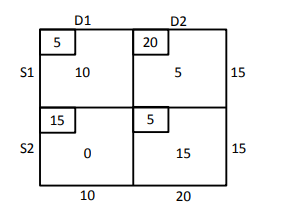
\includegraphics[width=0.75\columnwidth]{chapters/10/7/2/4/figs/fig.png}
 \end{center}
\caption{}
\label{fig:10/7/2/4Fig1}
\end{figure}
\fi

\item Find the position vector of the mid point of the vector joining the points $\vec{P}$(2, 3, 4)
and $\vec{Q}$(4, 1, –2).
\\
\solution
		\begin{enumerate}[label=\thesubsection.\arabic*,ref=\thesubsection.\theenumi]
\item Find the coordinates of the point which divides the join of $(-1,7) $ and $ (4,-3)$ in the ratio 2:3.
	\\
		\solution
	\input{chapters/10/7/2/1/section.tex}
\item Find the coordinates of the point $\vec{R}$ on the line segment joining the points $\vec{P}(-1,3)$ and $\vec{Q}(2,5)$ such that $PR=\frac{3}{5}PQ$.
\item Find the ratio in which the point $\vec{P}\brak{\frac{3}{4},\frac{5}{12}}$ divides the line segment joining the points $\vec{A}\brak{\frac{1}{2},\frac{3}{2}}$ and $ \vec{B}(2,-5)$.
\item Find the coordinates of the point which divides the line segment joining the points $(4,-3)$ and $(8,5)$ in the ratio $3:1$ internally.
\item Find the coordinates of the point $\vec{P}$ on $AD$ such that $AP : PD = 2 : 1$.
\item If the point $\vec{P} (2, 1)$ lies on the line segment joining points $\vec{A} (4, 2)$  and $ \vec{B} (8, 4)$,
then
\begin{enumerate}
	\item $AP =\frac{1}{3}{AB}$ 
\item ${AP}={PE}$
\item ${PB}=\frac{1}{3}{AB}$
\item${AP}=\frac{1}{2}{AB}$
 \end{enumerate}
\item Find the ratio in which the line segment joining the points $(-3,10)$  and  $(6,-8)$  is divided by $ (-1,6)$.
	\\
		\solution
	\input{chapters/10/7/2/4/section.tex}
\item Find the position vector of the mid point of the vector joining the points $\vec{P}$(2, 3, 4)
and $\vec{Q}$(4, 1, –2).
\\
\solution
		\input{chapters/12/10/2/16/section.tex}
\item Let $\vec{A}(4, 2), \vec{B}(6, 5)$  and $ \vec{C}(1, 4)$ be the vertices of $\triangle ABC$.
\begin{enumerate}
\item If $\vec{A}$ and  $\vec{B}$ are $(-2,-2)$ and  $(2,-4)$, respectively, find the coordinates of $\vec{P}$ such that $AP= \frac {3}{7}AB$  and $ \vec{P}$ lies on the line segment $AB$.
	\\
		\solution
	\input{chapters/10/7/2/8/section.tex}
\item Find the coordinates of the points which divide the line segment joining $A(-2,2)$  and  $\vec{B}(2,8)$ into four equal parts.
	\\
		\solution
	\input{chapters/10/7/2/9/section.tex}
\item In what ratio does the point $(-4,6)$ divide the line segment joining the points $\vec{A}(-6,0)$ and $\vec{B}(3,-8)$?
\item Given that $\vec{P}(3,2,-4), \vec{Q}(5,4,-6)$ and $\vec{R}(9,8,-10)$ are collinear. Find the ratio in which $\vec{Q}$ divides $PR$.
\item Points $\vec{A}(-6,10),\vec{B}(-4,6)$  and  $\vec{C}(3,-8)$ are collinear such that $AB=  \frac{2}{9}AC$.
\item The point which divides the line segment joining the points $\vec{P} (7, –6) $  and  $\vec{Q}(3, 4)$ in the 
ratio 1 : 2 internally lies in  which quadrant?
\item Find the coordinates of the points of trisection of the line segment joining $(4,-1)$  and  $(-2,3)$.
	\\
		\solution
	\input{chapters/10/7/2/2/section.tex}
\item Find the coordinates of the points which trisect the line segment joining the points $\vec{P}(4,2,-6)$ and $\vec{Q}(10,-16,6)$.
\item Find the coordinates of the points of trisection (i.e. points dividing to three equal parts) of the line segment joining the points $\vec{A}(2,-2)$ and $\vec{B}(-7,4)$.
\item Point $\vec{P}(5,-3)$ is one of the two points of trisection of line segment joining the points $\vec{A}(7,-2)$ and $\vec{B}(1,-5)$
\item Find the position vector of a point $\vec{R}$ which divides the line joining two points $\vec{P}$
and $\vec{Q}$ whose position vectors are $\hat{i}+2\hat{j}-\hat{k}$ and $-\hat{i}+\hat{j}+\hat{k}$ respectively, in the
ratio 2 : 1
\begin{enumerate}
    \item  internally
    \item  externally
\end{enumerate}
%\solution
%		\input{chapters/12/10/2/15/section.tex}
\item Find the coordinates of the point which divides the line segment joining the points which divides the line segment joining  the points $(-2,3,5)$ and $(1,-4,6)$ in the ratio 
\begin{enumerate}
\item $2:3$ internally,
\item $2:3$ externally
\end{enumerate}
\item Find the coordinates of the point which divides the line segment joining the points $(1,-2,3)$ and $(3,4,-5)$ in the ratio $2:3$
\begin{enumerate}
\item internally, and
\item externally
\end{enumerate}
\item Consider two points $\vec{P}$ and $\vec{Q}$ with position vectors $\overrightarrow{OP} = 3\overrightarrow{a}-2\overrightarrow{b}$ and $\overrightarrow{OQ}=\overrightarrow{a}+\overrightarrow{b}$. Find the position vector of a point $\vec{R}$ which divides the line joining $\vec{P}$ and $\vec{Q}$ in the ratio $2:1$, 
\begin{enumerate}
\item internally, and 
\item externally.
\end{enumerate}
\item The median from $\vec{A}$ meets $BC$ at $\vec{D}$. Find the coordinates of the point $\vec{D}$.
\item Find the coordinates of points $\vec{Q}$ and $\vec{R}$ on medians $BE$ and $CF$ respectively such that $BQ : QE = 2 : 1$  and  $CR : RF = 2 : 1$.
\item What do you observe?
\item If $\vec{A}, \vec{B}$ and $\vec{C}$  are the vertices of $\triangle ABC$, find the coordinates of the centroid of the triangle.
\end{enumerate}
\solution
	\input{chapters/10/7/4/7/section.tex}
\item If $\vec{P}(9a-2,-b)$ divides line segment joining $\vec{A}(3a+1,-3)$ and $\vec{B}(8a,5)$ in the ratio 3:1, find the values of $a$ and $b$.
\item Find the position vector of a point $\vec{R}$ which divides the line joining two points $\vec{P}$ and $\vec{Q}$ whose position vectors are $2\vec{a}+\vec{b}$ and $\vec{a}-3\vec{b}$ externally in the ratio $1:2$.
\item The position vector of the point which divides the join of points 2$\vec{a}$-3$\vec{b}$ $\text{and}$ $\vec{a}+\vec{b}$ in the ratio 3:1 is \rule{1cm}{0.1pt}.
\item If $\vec{a}$ and $\vec{b}$ are the postion vectors of $\vec{A}$ and $\vec{B}$, respectively, find the position vector of a point $\vec{C}$ in $BA$ produced such that $BC=1.5BA$.
\item Find the position vector of a point $\vec{R}$ which divides the line joining two points $\vec{P}$ and $\vec{Q}$ whose position vectors are $(2\vec{a}+\vec{b})$ and $(\vec{a}-3\vec{b})$
externally in the ratio 1 : 2. Also, show that $\vec{P}$ is the mid point of the line segment $RQ$.
\end{enumerate}

\item Let $\vec{A}(4, 2), \vec{B}(6, 5)$  and $ \vec{C}(1, 4)$ be the vertices of $\triangle ABC$.
\begin{enumerate}
\item If $\vec{A}$ and  $\vec{B}$ are $(-2,-2)$ and  $(2,-4)$, respectively, find the coordinates of $\vec{P}$ such that $AP= \frac {3}{7}AB$  and $ \vec{P}$ lies on the line segment $AB$.
	\\
		\solution
	\begin{enumerate}[label=\thesubsection.\arabic*,ref=\thesubsection.\theenumi]
\item Find the coordinates of the point which divides the join of $(-1,7) $ and $ (4,-3)$ in the ratio 2:3.
	\\
		\solution
	\input{chapters/10/7/2/1/section.tex}
\item Find the coordinates of the point $\vec{R}$ on the line segment joining the points $\vec{P}(-1,3)$ and $\vec{Q}(2,5)$ such that $PR=\frac{3}{5}PQ$.
\item Find the ratio in which the point $\vec{P}\brak{\frac{3}{4},\frac{5}{12}}$ divides the line segment joining the points $\vec{A}\brak{\frac{1}{2},\frac{3}{2}}$ and $ \vec{B}(2,-5)$.
\item Find the coordinates of the point which divides the line segment joining the points $(4,-3)$ and $(8,5)$ in the ratio $3:1$ internally.
\item Find the coordinates of the point $\vec{P}$ on $AD$ such that $AP : PD = 2 : 1$.
\item If the point $\vec{P} (2, 1)$ lies on the line segment joining points $\vec{A} (4, 2)$  and $ \vec{B} (8, 4)$,
then
\begin{enumerate}
	\item $AP =\frac{1}{3}{AB}$ 
\item ${AP}={PE}$
\item ${PB}=\frac{1}{3}{AB}$
\item${AP}=\frac{1}{2}{AB}$
 \end{enumerate}
\item Find the ratio in which the line segment joining the points $(-3,10)$  and  $(6,-8)$  is divided by $ (-1,6)$.
	\\
		\solution
	\input{chapters/10/7/2/4/section.tex}
\item Find the position vector of the mid point of the vector joining the points $\vec{P}$(2, 3, 4)
and $\vec{Q}$(4, 1, –2).
\\
\solution
		\input{chapters/12/10/2/16/section.tex}
\item Let $\vec{A}(4, 2), \vec{B}(6, 5)$  and $ \vec{C}(1, 4)$ be the vertices of $\triangle ABC$.
\begin{enumerate}
\item If $\vec{A}$ and  $\vec{B}$ are $(-2,-2)$ and  $(2,-4)$, respectively, find the coordinates of $\vec{P}$ such that $AP= \frac {3}{7}AB$  and $ \vec{P}$ lies on the line segment $AB$.
	\\
		\solution
	\input{chapters/10/7/2/8/section.tex}
\item Find the coordinates of the points which divide the line segment joining $A(-2,2)$  and  $\vec{B}(2,8)$ into four equal parts.
	\\
		\solution
	\input{chapters/10/7/2/9/section.tex}
\item In what ratio does the point $(-4,6)$ divide the line segment joining the points $\vec{A}(-6,0)$ and $\vec{B}(3,-8)$?
\item Given that $\vec{P}(3,2,-4), \vec{Q}(5,4,-6)$ and $\vec{R}(9,8,-10)$ are collinear. Find the ratio in which $\vec{Q}$ divides $PR$.
\item Points $\vec{A}(-6,10),\vec{B}(-4,6)$  and  $\vec{C}(3,-8)$ are collinear such that $AB=  \frac{2}{9}AC$.
\item The point which divides the line segment joining the points $\vec{P} (7, –6) $  and  $\vec{Q}(3, 4)$ in the 
ratio 1 : 2 internally lies in  which quadrant?
\item Find the coordinates of the points of trisection of the line segment joining $(4,-1)$  and  $(-2,3)$.
	\\
		\solution
	\input{chapters/10/7/2/2/section.tex}
\item Find the coordinates of the points which trisect the line segment joining the points $\vec{P}(4,2,-6)$ and $\vec{Q}(10,-16,6)$.
\item Find the coordinates of the points of trisection (i.e. points dividing to three equal parts) of the line segment joining the points $\vec{A}(2,-2)$ and $\vec{B}(-7,4)$.
\item Point $\vec{P}(5,-3)$ is one of the two points of trisection of line segment joining the points $\vec{A}(7,-2)$ and $\vec{B}(1,-5)$
\item Find the position vector of a point $\vec{R}$ which divides the line joining two points $\vec{P}$
and $\vec{Q}$ whose position vectors are $\hat{i}+2\hat{j}-\hat{k}$ and $-\hat{i}+\hat{j}+\hat{k}$ respectively, in the
ratio 2 : 1
\begin{enumerate}
    \item  internally
    \item  externally
\end{enumerate}
%\solution
%		\input{chapters/12/10/2/15/section.tex}
\item Find the coordinates of the point which divides the line segment joining the points which divides the line segment joining  the points $(-2,3,5)$ and $(1,-4,6)$ in the ratio 
\begin{enumerate}
\item $2:3$ internally,
\item $2:3$ externally
\end{enumerate}
\item Find the coordinates of the point which divides the line segment joining the points $(1,-2,3)$ and $(3,4,-5)$ in the ratio $2:3$
\begin{enumerate}
\item internally, and
\item externally
\end{enumerate}
\item Consider two points $\vec{P}$ and $\vec{Q}$ with position vectors $\overrightarrow{OP} = 3\overrightarrow{a}-2\overrightarrow{b}$ and $\overrightarrow{OQ}=\overrightarrow{a}+\overrightarrow{b}$. Find the position vector of a point $\vec{R}$ which divides the line joining $\vec{P}$ and $\vec{Q}$ in the ratio $2:1$, 
\begin{enumerate}
\item internally, and 
\item externally.
\end{enumerate}
\item The median from $\vec{A}$ meets $BC$ at $\vec{D}$. Find the coordinates of the point $\vec{D}$.
\item Find the coordinates of points $\vec{Q}$ and $\vec{R}$ on medians $BE$ and $CF$ respectively such that $BQ : QE = 2 : 1$  and  $CR : RF = 2 : 1$.
\item What do you observe?
\item If $\vec{A}, \vec{B}$ and $\vec{C}$  are the vertices of $\triangle ABC$, find the coordinates of the centroid of the triangle.
\end{enumerate}
\solution
	\input{chapters/10/7/4/7/section.tex}
\item If $\vec{P}(9a-2,-b)$ divides line segment joining $\vec{A}(3a+1,-3)$ and $\vec{B}(8a,5)$ in the ratio 3:1, find the values of $a$ and $b$.
\item Find the position vector of a point $\vec{R}$ which divides the line joining two points $\vec{P}$ and $\vec{Q}$ whose position vectors are $2\vec{a}+\vec{b}$ and $\vec{a}-3\vec{b}$ externally in the ratio $1:2$.
\item The position vector of the point which divides the join of points 2$\vec{a}$-3$\vec{b}$ $\text{and}$ $\vec{a}+\vec{b}$ in the ratio 3:1 is \rule{1cm}{0.1pt}.
\item If $\vec{a}$ and $\vec{b}$ are the postion vectors of $\vec{A}$ and $\vec{B}$, respectively, find the position vector of a point $\vec{C}$ in $BA$ produced such that $BC=1.5BA$.
\item Find the position vector of a point $\vec{R}$ which divides the line joining two points $\vec{P}$ and $\vec{Q}$ whose position vectors are $(2\vec{a}+\vec{b})$ and $(\vec{a}-3\vec{b})$
externally in the ratio 1 : 2. Also, show that $\vec{P}$ is the mid point of the line segment $RQ$.
\end{enumerate}

\item Find the coordinates of the points which divide the line segment joining $A(-2,2)$  and  $\vec{B}(2,8)$ into four equal parts.
	\\
		\solution
	\begin{enumerate}[label=\thesubsection.\arabic*,ref=\thesubsection.\theenumi]
\item Find the coordinates of the point which divides the join of $(-1,7) $ and $ (4,-3)$ in the ratio 2:3.
	\\
		\solution
	\input{chapters/10/7/2/1/section.tex}
\item Find the coordinates of the point $\vec{R}$ on the line segment joining the points $\vec{P}(-1,3)$ and $\vec{Q}(2,5)$ such that $PR=\frac{3}{5}PQ$.
\item Find the ratio in which the point $\vec{P}\brak{\frac{3}{4},\frac{5}{12}}$ divides the line segment joining the points $\vec{A}\brak{\frac{1}{2},\frac{3}{2}}$ and $ \vec{B}(2,-5)$.
\item Find the coordinates of the point which divides the line segment joining the points $(4,-3)$ and $(8,5)$ in the ratio $3:1$ internally.
\item Find the coordinates of the point $\vec{P}$ on $AD$ such that $AP : PD = 2 : 1$.
\item If the point $\vec{P} (2, 1)$ lies on the line segment joining points $\vec{A} (4, 2)$  and $ \vec{B} (8, 4)$,
then
\begin{enumerate}
	\item $AP =\frac{1}{3}{AB}$ 
\item ${AP}={PE}$
\item ${PB}=\frac{1}{3}{AB}$
\item${AP}=\frac{1}{2}{AB}$
 \end{enumerate}
\item Find the ratio in which the line segment joining the points $(-3,10)$  and  $(6,-8)$  is divided by $ (-1,6)$.
	\\
		\solution
	\input{chapters/10/7/2/4/section.tex}
\item Find the position vector of the mid point of the vector joining the points $\vec{P}$(2, 3, 4)
and $\vec{Q}$(4, 1, –2).
\\
\solution
		\input{chapters/12/10/2/16/section.tex}
\item Let $\vec{A}(4, 2), \vec{B}(6, 5)$  and $ \vec{C}(1, 4)$ be the vertices of $\triangle ABC$.
\begin{enumerate}
\item If $\vec{A}$ and  $\vec{B}$ are $(-2,-2)$ and  $(2,-4)$, respectively, find the coordinates of $\vec{P}$ such that $AP= \frac {3}{7}AB$  and $ \vec{P}$ lies on the line segment $AB$.
	\\
		\solution
	\input{chapters/10/7/2/8/section.tex}
\item Find the coordinates of the points which divide the line segment joining $A(-2,2)$  and  $\vec{B}(2,8)$ into four equal parts.
	\\
		\solution
	\input{chapters/10/7/2/9/section.tex}
\item In what ratio does the point $(-4,6)$ divide the line segment joining the points $\vec{A}(-6,0)$ and $\vec{B}(3,-8)$?
\item Given that $\vec{P}(3,2,-4), \vec{Q}(5,4,-6)$ and $\vec{R}(9,8,-10)$ are collinear. Find the ratio in which $\vec{Q}$ divides $PR$.
\item Points $\vec{A}(-6,10),\vec{B}(-4,6)$  and  $\vec{C}(3,-8)$ are collinear such that $AB=  \frac{2}{9}AC$.
\item The point which divides the line segment joining the points $\vec{P} (7, –6) $  and  $\vec{Q}(3, 4)$ in the 
ratio 1 : 2 internally lies in  which quadrant?
\item Find the coordinates of the points of trisection of the line segment joining $(4,-1)$  and  $(-2,3)$.
	\\
		\solution
	\input{chapters/10/7/2/2/section.tex}
\item Find the coordinates of the points which trisect the line segment joining the points $\vec{P}(4,2,-6)$ and $\vec{Q}(10,-16,6)$.
\item Find the coordinates of the points of trisection (i.e. points dividing to three equal parts) of the line segment joining the points $\vec{A}(2,-2)$ and $\vec{B}(-7,4)$.
\item Point $\vec{P}(5,-3)$ is one of the two points of trisection of line segment joining the points $\vec{A}(7,-2)$ and $\vec{B}(1,-5)$
\item Find the position vector of a point $\vec{R}$ which divides the line joining two points $\vec{P}$
and $\vec{Q}$ whose position vectors are $\hat{i}+2\hat{j}-\hat{k}$ and $-\hat{i}+\hat{j}+\hat{k}$ respectively, in the
ratio 2 : 1
\begin{enumerate}
    \item  internally
    \item  externally
\end{enumerate}
%\solution
%		\input{chapters/12/10/2/15/section.tex}
\item Find the coordinates of the point which divides the line segment joining the points which divides the line segment joining  the points $(-2,3,5)$ and $(1,-4,6)$ in the ratio 
\begin{enumerate}
\item $2:3$ internally,
\item $2:3$ externally
\end{enumerate}
\item Find the coordinates of the point which divides the line segment joining the points $(1,-2,3)$ and $(3,4,-5)$ in the ratio $2:3$
\begin{enumerate}
\item internally, and
\item externally
\end{enumerate}
\item Consider two points $\vec{P}$ and $\vec{Q}$ with position vectors $\overrightarrow{OP} = 3\overrightarrow{a}-2\overrightarrow{b}$ and $\overrightarrow{OQ}=\overrightarrow{a}+\overrightarrow{b}$. Find the position vector of a point $\vec{R}$ which divides the line joining $\vec{P}$ and $\vec{Q}$ in the ratio $2:1$, 
\begin{enumerate}
\item internally, and 
\item externally.
\end{enumerate}
\item The median from $\vec{A}$ meets $BC$ at $\vec{D}$. Find the coordinates of the point $\vec{D}$.
\item Find the coordinates of points $\vec{Q}$ and $\vec{R}$ on medians $BE$ and $CF$ respectively such that $BQ : QE = 2 : 1$  and  $CR : RF = 2 : 1$.
\item What do you observe?
\item If $\vec{A}, \vec{B}$ and $\vec{C}$  are the vertices of $\triangle ABC$, find the coordinates of the centroid of the triangle.
\end{enumerate}
\solution
	\input{chapters/10/7/4/7/section.tex}
\item If $\vec{P}(9a-2,-b)$ divides line segment joining $\vec{A}(3a+1,-3)$ and $\vec{B}(8a,5)$ in the ratio 3:1, find the values of $a$ and $b$.
\item Find the position vector of a point $\vec{R}$ which divides the line joining two points $\vec{P}$ and $\vec{Q}$ whose position vectors are $2\vec{a}+\vec{b}$ and $\vec{a}-3\vec{b}$ externally in the ratio $1:2$.
\item The position vector of the point which divides the join of points 2$\vec{a}$-3$\vec{b}$ $\text{and}$ $\vec{a}+\vec{b}$ in the ratio 3:1 is \rule{1cm}{0.1pt}.
\item If $\vec{a}$ and $\vec{b}$ are the postion vectors of $\vec{A}$ and $\vec{B}$, respectively, find the position vector of a point $\vec{C}$ in $BA$ produced such that $BC=1.5BA$.
\item Find the position vector of a point $\vec{R}$ which divides the line joining two points $\vec{P}$ and $\vec{Q}$ whose position vectors are $(2\vec{a}+\vec{b})$ and $(\vec{a}-3\vec{b})$
externally in the ratio 1 : 2. Also, show that $\vec{P}$ is the mid point of the line segment $RQ$.
\end{enumerate}

\item In what ratio does the point $(-4,6)$ divide the line segment joining the points $\vec{A}(-6,0)$ and $\vec{B}(3,-8)$?
\item Given that $\vec{P}(3,2,-4), \vec{Q}(5,4,-6)$ and $\vec{R}(9,8,-10)$ are collinear. Find the ratio in which $\vec{Q}$ divides $PR$.
\item Points $\vec{A}(-6,10),\vec{B}(-4,6)$  and  $\vec{C}(3,-8)$ are collinear such that $AB=  \frac{2}{9}AC$.
\item The point which divides the line segment joining the points $\vec{P} (7, –6) $  and  $\vec{Q}(3, 4)$ in the 
ratio 1 : 2 internally lies in  which quadrant?
\item Find the coordinates of the points of trisection of the line segment joining $(4,-1)$  and  $(-2,3)$.
	\\
		\solution
	Using section formula,
\begin{align}
\vec{R}=\frac{1}{1+\frac{1}{2}}\brak{\myvec{4\\-1}+\frac{1}{2}\myvec{-2\\3}}
=\myvec{2\\ \frac{1}{3}}\\
\vec{S}=\frac{1}{1+\frac{2}{1}}\brak{\myvec{4\\-1}+\frac{2}{1}\myvec{-2\\3}}
=\myvec{0\\ \frac{5}{3}}
\end{align}
which are the desired points of trisection.
\iffalse
See
		\figref{fig:chapters/10/7/2/2/Figure}
\begin{figure}[H]
\centering
\includegraphics[width=0.75\columnwidth]{chapters/10/7/2/2/figs/dj.pdf}
\caption{}
		\label{fig:chapters/10/7/2/2/Figure}
\end{figure}
\fi

\item Find the coordinates of the points which trisect the line segment joining the points $\vec{P}(4,2,-6)$ and $\vec{Q}(10,-16,6)$.
\item Find the coordinates of the points of trisection (i.e. points dividing to three equal parts) of the line segment joining the points $\vec{A}(2,-2)$ and $\vec{B}(-7,4)$.
\item Point $\vec{P}(5,-3)$ is one of the two points of trisection of line segment joining the points $\vec{A}(7,-2)$ and $\vec{B}(1,-5)$
\item Find the position vector of a point $\vec{R}$ which divides the line joining two points $\vec{P}$
and $\vec{Q}$ whose position vectors are $\hat{i}+2\hat{j}-\hat{k}$ and $-\hat{i}+\hat{j}+\hat{k}$ respectively, in the
ratio 2 : 1
\begin{enumerate}
    \item  internally
    \item  externally
\end{enumerate}
%\solution
%		\begin{enumerate}[label=\thesubsection.\arabic*,ref=\thesubsection.\theenumi]
\item Find the coordinates of the point which divides the join of $(-1,7) $ and $ (4,-3)$ in the ratio 2:3.
	\\
		\solution
	\input{chapters/10/7/2/1/section.tex}
\item Find the coordinates of the point $\vec{R}$ on the line segment joining the points $\vec{P}(-1,3)$ and $\vec{Q}(2,5)$ such that $PR=\frac{3}{5}PQ$.
\item Find the ratio in which the point $\vec{P}\brak{\frac{3}{4},\frac{5}{12}}$ divides the line segment joining the points $\vec{A}\brak{\frac{1}{2},\frac{3}{2}}$ and $ \vec{B}(2,-5)$.
\item Find the coordinates of the point which divides the line segment joining the points $(4,-3)$ and $(8,5)$ in the ratio $3:1$ internally.
\item Find the coordinates of the point $\vec{P}$ on $AD$ such that $AP : PD = 2 : 1$.
\item If the point $\vec{P} (2, 1)$ lies on the line segment joining points $\vec{A} (4, 2)$  and $ \vec{B} (8, 4)$,
then
\begin{enumerate}
	\item $AP =\frac{1}{3}{AB}$ 
\item ${AP}={PE}$
\item ${PB}=\frac{1}{3}{AB}$
\item${AP}=\frac{1}{2}{AB}$
 \end{enumerate}
\item Find the ratio in which the line segment joining the points $(-3,10)$  and  $(6,-8)$  is divided by $ (-1,6)$.
	\\
		\solution
	\input{chapters/10/7/2/4/section.tex}
\item Find the position vector of the mid point of the vector joining the points $\vec{P}$(2, 3, 4)
and $\vec{Q}$(4, 1, –2).
\\
\solution
		\input{chapters/12/10/2/16/section.tex}
\item Let $\vec{A}(4, 2), \vec{B}(6, 5)$  and $ \vec{C}(1, 4)$ be the vertices of $\triangle ABC$.
\begin{enumerate}
\item If $\vec{A}$ and  $\vec{B}$ are $(-2,-2)$ and  $(2,-4)$, respectively, find the coordinates of $\vec{P}$ such that $AP= \frac {3}{7}AB$  and $ \vec{P}$ lies on the line segment $AB$.
	\\
		\solution
	\input{chapters/10/7/2/8/section.tex}
\item Find the coordinates of the points which divide the line segment joining $A(-2,2)$  and  $\vec{B}(2,8)$ into four equal parts.
	\\
		\solution
	\input{chapters/10/7/2/9/section.tex}
\item In what ratio does the point $(-4,6)$ divide the line segment joining the points $\vec{A}(-6,0)$ and $\vec{B}(3,-8)$?
\item Given that $\vec{P}(3,2,-4), \vec{Q}(5,4,-6)$ and $\vec{R}(9,8,-10)$ are collinear. Find the ratio in which $\vec{Q}$ divides $PR$.
\item Points $\vec{A}(-6,10),\vec{B}(-4,6)$  and  $\vec{C}(3,-8)$ are collinear such that $AB=  \frac{2}{9}AC$.
\item The point which divides the line segment joining the points $\vec{P} (7, –6) $  and  $\vec{Q}(3, 4)$ in the 
ratio 1 : 2 internally lies in  which quadrant?
\item Find the coordinates of the points of trisection of the line segment joining $(4,-1)$  and  $(-2,3)$.
	\\
		\solution
	\input{chapters/10/7/2/2/section.tex}
\item Find the coordinates of the points which trisect the line segment joining the points $\vec{P}(4,2,-6)$ and $\vec{Q}(10,-16,6)$.
\item Find the coordinates of the points of trisection (i.e. points dividing to three equal parts) of the line segment joining the points $\vec{A}(2,-2)$ and $\vec{B}(-7,4)$.
\item Point $\vec{P}(5,-3)$ is one of the two points of trisection of line segment joining the points $\vec{A}(7,-2)$ and $\vec{B}(1,-5)$
\item Find the position vector of a point $\vec{R}$ which divides the line joining two points $\vec{P}$
and $\vec{Q}$ whose position vectors are $\hat{i}+2\hat{j}-\hat{k}$ and $-\hat{i}+\hat{j}+\hat{k}$ respectively, in the
ratio 2 : 1
\begin{enumerate}
    \item  internally
    \item  externally
\end{enumerate}
%\solution
%		\input{chapters/12/10/2/15/section.tex}
\item Find the coordinates of the point which divides the line segment joining the points which divides the line segment joining  the points $(-2,3,5)$ and $(1,-4,6)$ in the ratio 
\begin{enumerate}
\item $2:3$ internally,
\item $2:3$ externally
\end{enumerate}
\item Find the coordinates of the point which divides the line segment joining the points $(1,-2,3)$ and $(3,4,-5)$ in the ratio $2:3$
\begin{enumerate}
\item internally, and
\item externally
\end{enumerate}
\item Consider two points $\vec{P}$ and $\vec{Q}$ with position vectors $\overrightarrow{OP} = 3\overrightarrow{a}-2\overrightarrow{b}$ and $\overrightarrow{OQ}=\overrightarrow{a}+\overrightarrow{b}$. Find the position vector of a point $\vec{R}$ which divides the line joining $\vec{P}$ and $\vec{Q}$ in the ratio $2:1$, 
\begin{enumerate}
\item internally, and 
\item externally.
\end{enumerate}
\item The median from $\vec{A}$ meets $BC$ at $\vec{D}$. Find the coordinates of the point $\vec{D}$.
\item Find the coordinates of points $\vec{Q}$ and $\vec{R}$ on medians $BE$ and $CF$ respectively such that $BQ : QE = 2 : 1$  and  $CR : RF = 2 : 1$.
\item What do you observe?
\item If $\vec{A}, \vec{B}$ and $\vec{C}$  are the vertices of $\triangle ABC$, find the coordinates of the centroid of the triangle.
\end{enumerate}
\solution
	\input{chapters/10/7/4/7/section.tex}
\item If $\vec{P}(9a-2,-b)$ divides line segment joining $\vec{A}(3a+1,-3)$ and $\vec{B}(8a,5)$ in the ratio 3:1, find the values of $a$ and $b$.
\item Find the position vector of a point $\vec{R}$ which divides the line joining two points $\vec{P}$ and $\vec{Q}$ whose position vectors are $2\vec{a}+\vec{b}$ and $\vec{a}-3\vec{b}$ externally in the ratio $1:2$.
\item The position vector of the point which divides the join of points 2$\vec{a}$-3$\vec{b}$ $\text{and}$ $\vec{a}+\vec{b}$ in the ratio 3:1 is \rule{1cm}{0.1pt}.
\item If $\vec{a}$ and $\vec{b}$ are the postion vectors of $\vec{A}$ and $\vec{B}$, respectively, find the position vector of a point $\vec{C}$ in $BA$ produced such that $BC=1.5BA$.
\item Find the position vector of a point $\vec{R}$ which divides the line joining two points $\vec{P}$ and $\vec{Q}$ whose position vectors are $(2\vec{a}+\vec{b})$ and $(\vec{a}-3\vec{b})$
externally in the ratio 1 : 2. Also, show that $\vec{P}$ is the mid point of the line segment $RQ$.
\end{enumerate}

\item Find the coordinates of the point which divides the line segment joining the points which divides the line segment joining  the points $(-2,3,5)$ and $(1,-4,6)$ in the ratio 
\begin{enumerate}
\item $2:3$ internally,
\item $2:3$ externally
\end{enumerate}
\item Find the coordinates of the point which divides the line segment joining the points $(1,-2,3)$ and $(3,4,-5)$ in the ratio $2:3$
\begin{enumerate}
\item internally, and
\item externally
\end{enumerate}
\item Consider two points $\vec{P}$ and $\vec{Q}$ with position vectors $\overrightarrow{OP} = 3\overrightarrow{a}-2\overrightarrow{b}$ and $\overrightarrow{OQ}=\overrightarrow{a}+\overrightarrow{b}$. Find the position vector of a point $\vec{R}$ which divides the line joining $\vec{P}$ and $\vec{Q}$ in the ratio $2:1$, 
\begin{enumerate}
\item internally, and 
\item externally.
\end{enumerate}
\item The median from $\vec{A}$ meets $BC$ at $\vec{D}$. Find the coordinates of the point $\vec{D}$.
\item Find the coordinates of points $\vec{Q}$ and $\vec{R}$ on medians $BE$ and $CF$ respectively such that $BQ : QE = 2 : 1$  and  $CR : RF = 2 : 1$.
\item What do you observe?
\item If $\vec{A}, \vec{B}$ and $\vec{C}$  are the vertices of $\triangle ABC$, find the coordinates of the centroid of the triangle.
\end{enumerate}
\solution
	\begin{enumerate}[label=\thesubsection.\arabic*,ref=\thesubsection.\theenumi]
\item Find the coordinates of the point which divides the join of $(-1,7) $ and $ (4,-3)$ in the ratio 2:3.
	\\
		\solution
	\input{chapters/10/7/2/1/section.tex}
\item Find the coordinates of the point $\vec{R}$ on the line segment joining the points $\vec{P}(-1,3)$ and $\vec{Q}(2,5)$ such that $PR=\frac{3}{5}PQ$.
\item Find the ratio in which the point $\vec{P}\brak{\frac{3}{4},\frac{5}{12}}$ divides the line segment joining the points $\vec{A}\brak{\frac{1}{2},\frac{3}{2}}$ and $ \vec{B}(2,-5)$.
\item Find the coordinates of the point which divides the line segment joining the points $(4,-3)$ and $(8,5)$ in the ratio $3:1$ internally.
\item Find the coordinates of the point $\vec{P}$ on $AD$ such that $AP : PD = 2 : 1$.
\item If the point $\vec{P} (2, 1)$ lies on the line segment joining points $\vec{A} (4, 2)$  and $ \vec{B} (8, 4)$,
then
\begin{enumerate}
	\item $AP =\frac{1}{3}{AB}$ 
\item ${AP}={PE}$
\item ${PB}=\frac{1}{3}{AB}$
\item${AP}=\frac{1}{2}{AB}$
 \end{enumerate}
\item Find the ratio in which the line segment joining the points $(-3,10)$  and  $(6,-8)$  is divided by $ (-1,6)$.
	\\
		\solution
	\input{chapters/10/7/2/4/section.tex}
\item Find the position vector of the mid point of the vector joining the points $\vec{P}$(2, 3, 4)
and $\vec{Q}$(4, 1, –2).
\\
\solution
		\input{chapters/12/10/2/16/section.tex}
\item Let $\vec{A}(4, 2), \vec{B}(6, 5)$  and $ \vec{C}(1, 4)$ be the vertices of $\triangle ABC$.
\begin{enumerate}
\item If $\vec{A}$ and  $\vec{B}$ are $(-2,-2)$ and  $(2,-4)$, respectively, find the coordinates of $\vec{P}$ such that $AP= \frac {3}{7}AB$  and $ \vec{P}$ lies on the line segment $AB$.
	\\
		\solution
	\input{chapters/10/7/2/8/section.tex}
\item Find the coordinates of the points which divide the line segment joining $A(-2,2)$  and  $\vec{B}(2,8)$ into four equal parts.
	\\
		\solution
	\input{chapters/10/7/2/9/section.tex}
\item In what ratio does the point $(-4,6)$ divide the line segment joining the points $\vec{A}(-6,0)$ and $\vec{B}(3,-8)$?
\item Given that $\vec{P}(3,2,-4), \vec{Q}(5,4,-6)$ and $\vec{R}(9,8,-10)$ are collinear. Find the ratio in which $\vec{Q}$ divides $PR$.
\item Points $\vec{A}(-6,10),\vec{B}(-4,6)$  and  $\vec{C}(3,-8)$ are collinear such that $AB=  \frac{2}{9}AC$.
\item The point which divides the line segment joining the points $\vec{P} (7, –6) $  and  $\vec{Q}(3, 4)$ in the 
ratio 1 : 2 internally lies in  which quadrant?
\item Find the coordinates of the points of trisection of the line segment joining $(4,-1)$  and  $(-2,3)$.
	\\
		\solution
	\input{chapters/10/7/2/2/section.tex}
\item Find the coordinates of the points which trisect the line segment joining the points $\vec{P}(4,2,-6)$ and $\vec{Q}(10,-16,6)$.
\item Find the coordinates of the points of trisection (i.e. points dividing to three equal parts) of the line segment joining the points $\vec{A}(2,-2)$ and $\vec{B}(-7,4)$.
\item Point $\vec{P}(5,-3)$ is one of the two points of trisection of line segment joining the points $\vec{A}(7,-2)$ and $\vec{B}(1,-5)$
\item Find the position vector of a point $\vec{R}$ which divides the line joining two points $\vec{P}$
and $\vec{Q}$ whose position vectors are $\hat{i}+2\hat{j}-\hat{k}$ and $-\hat{i}+\hat{j}+\hat{k}$ respectively, in the
ratio 2 : 1
\begin{enumerate}
    \item  internally
    \item  externally
\end{enumerate}
%\solution
%		\input{chapters/12/10/2/15/section.tex}
\item Find the coordinates of the point which divides the line segment joining the points which divides the line segment joining  the points $(-2,3,5)$ and $(1,-4,6)$ in the ratio 
\begin{enumerate}
\item $2:3$ internally,
\item $2:3$ externally
\end{enumerate}
\item Find the coordinates of the point which divides the line segment joining the points $(1,-2,3)$ and $(3,4,-5)$ in the ratio $2:3$
\begin{enumerate}
\item internally, and
\item externally
\end{enumerate}
\item Consider two points $\vec{P}$ and $\vec{Q}$ with position vectors $\overrightarrow{OP} = 3\overrightarrow{a}-2\overrightarrow{b}$ and $\overrightarrow{OQ}=\overrightarrow{a}+\overrightarrow{b}$. Find the position vector of a point $\vec{R}$ which divides the line joining $\vec{P}$ and $\vec{Q}$ in the ratio $2:1$, 
\begin{enumerate}
\item internally, and 
\item externally.
\end{enumerate}
\item The median from $\vec{A}$ meets $BC$ at $\vec{D}$. Find the coordinates of the point $\vec{D}$.
\item Find the coordinates of points $\vec{Q}$ and $\vec{R}$ on medians $BE$ and $CF$ respectively such that $BQ : QE = 2 : 1$  and  $CR : RF = 2 : 1$.
\item What do you observe?
\item If $\vec{A}, \vec{B}$ and $\vec{C}$  are the vertices of $\triangle ABC$, find the coordinates of the centroid of the triangle.
\end{enumerate}
\solution
	\input{chapters/10/7/4/7/section.tex}
\item If $\vec{P}(9a-2,-b)$ divides line segment joining $\vec{A}(3a+1,-3)$ and $\vec{B}(8a,5)$ in the ratio 3:1, find the values of $a$ and $b$.
\item Find the position vector of a point $\vec{R}$ which divides the line joining two points $\vec{P}$ and $\vec{Q}$ whose position vectors are $2\vec{a}+\vec{b}$ and $\vec{a}-3\vec{b}$ externally in the ratio $1:2$.
\item The position vector of the point which divides the join of points 2$\vec{a}$-3$\vec{b}$ $\text{and}$ $\vec{a}+\vec{b}$ in the ratio 3:1 is \rule{1cm}{0.1pt}.
\item If $\vec{a}$ and $\vec{b}$ are the postion vectors of $\vec{A}$ and $\vec{B}$, respectively, find the position vector of a point $\vec{C}$ in $BA$ produced such that $BC=1.5BA$.
\item Find the position vector of a point $\vec{R}$ which divides the line joining two points $\vec{P}$ and $\vec{Q}$ whose position vectors are $(2\vec{a}+\vec{b})$ and $(\vec{a}-3\vec{b})$
externally in the ratio 1 : 2. Also, show that $\vec{P}$ is the mid point of the line segment $RQ$.
\end{enumerate}

\item If $\vec{P}(9a-2,-b)$ divides line segment joining $\vec{A}(3a+1,-3)$ and $\vec{B}(8a,5)$ in the ratio 3:1, find the values of $a$ and $b$.
\item Find the position vector of a point $\vec{R}$ which divides the line joining two points $\vec{P}$ and $\vec{Q}$ whose position vectors are $2\vec{a}+\vec{b}$ and $\vec{a}-3\vec{b}$ externally in the ratio $1:2$.
\item The position vector of the point which divides the join of points 2$\vec{a}$-3$\vec{b}$ $\text{and}$ $\vec{a}+\vec{b}$ in the ratio 3:1 is \rule{1cm}{0.1pt}.
\item If $\vec{a}$ and $\vec{b}$ are the postion vectors of $\vec{A}$ and $\vec{B}$, respectively, find the position vector of a point $\vec{C}$ in $BA$ produced such that $BC=1.5BA$.
\item Find the position vector of a point $\vec{R}$ which divides the line joining two points $\vec{P}$ and $\vec{Q}$ whose position vectors are $(2\vec{a}+\vec{b})$ and $(\vec{a}-3\vec{b})$
externally in the ratio 1 : 2. Also, show that $\vec{P}$ is the mid point of the line segment $RQ$.
\end{enumerate}

\item Find the coordinates of the points which divide the line segment joining $A(-2,2)$  and  $\vec{B}(2,8)$ into four equal parts.
	\\
		\solution
	\begin{enumerate}[label=\thesubsection.\arabic*,ref=\thesubsection.\theenumi]
\item Find the coordinates of the point which divides the join of $(-1,7) $ and $ (4,-3)$ in the ratio 2:3.
	\\
		\solution
	\begin{enumerate}[label=\thesubsection.\arabic*,ref=\thesubsection.\theenumi]
\item Find the coordinates of the point which divides the join of $(-1,7) $ and $ (4,-3)$ in the ratio 2:3.
	\\
		\solution
	\input{chapters/10/7/2/1/section.tex}
\item Find the coordinates of the point $\vec{R}$ on the line segment joining the points $\vec{P}(-1,3)$ and $\vec{Q}(2,5)$ such that $PR=\frac{3}{5}PQ$.
\item Find the ratio in which the point $\vec{P}\brak{\frac{3}{4},\frac{5}{12}}$ divides the line segment joining the points $\vec{A}\brak{\frac{1}{2},\frac{3}{2}}$ and $ \vec{B}(2,-5)$.
\item Find the coordinates of the point which divides the line segment joining the points $(4,-3)$ and $(8,5)$ in the ratio $3:1$ internally.
\item Find the coordinates of the point $\vec{P}$ on $AD$ such that $AP : PD = 2 : 1$.
\item If the point $\vec{P} (2, 1)$ lies on the line segment joining points $\vec{A} (4, 2)$  and $ \vec{B} (8, 4)$,
then
\begin{enumerate}
	\item $AP =\frac{1}{3}{AB}$ 
\item ${AP}={PE}$
\item ${PB}=\frac{1}{3}{AB}$
\item${AP}=\frac{1}{2}{AB}$
 \end{enumerate}
\item Find the ratio in which the line segment joining the points $(-3,10)$  and  $(6,-8)$  is divided by $ (-1,6)$.
	\\
		\solution
	\input{chapters/10/7/2/4/section.tex}
\item Find the position vector of the mid point of the vector joining the points $\vec{P}$(2, 3, 4)
and $\vec{Q}$(4, 1, –2).
\\
\solution
		\input{chapters/12/10/2/16/section.tex}
\item Let $\vec{A}(4, 2), \vec{B}(6, 5)$  and $ \vec{C}(1, 4)$ be the vertices of $\triangle ABC$.
\begin{enumerate}
\item If $\vec{A}$ and  $\vec{B}$ are $(-2,-2)$ and  $(2,-4)$, respectively, find the coordinates of $\vec{P}$ such that $AP= \frac {3}{7}AB$  and $ \vec{P}$ lies on the line segment $AB$.
	\\
		\solution
	\input{chapters/10/7/2/8/section.tex}
\item Find the coordinates of the points which divide the line segment joining $A(-2,2)$  and  $\vec{B}(2,8)$ into four equal parts.
	\\
		\solution
	\input{chapters/10/7/2/9/section.tex}
\item In what ratio does the point $(-4,6)$ divide the line segment joining the points $\vec{A}(-6,0)$ and $\vec{B}(3,-8)$?
\item Given that $\vec{P}(3,2,-4), \vec{Q}(5,4,-6)$ and $\vec{R}(9,8,-10)$ are collinear. Find the ratio in which $\vec{Q}$ divides $PR$.
\item Points $\vec{A}(-6,10),\vec{B}(-4,6)$  and  $\vec{C}(3,-8)$ are collinear such that $AB=  \frac{2}{9}AC$.
\item The point which divides the line segment joining the points $\vec{P} (7, –6) $  and  $\vec{Q}(3, 4)$ in the 
ratio 1 : 2 internally lies in  which quadrant?
\item Find the coordinates of the points of trisection of the line segment joining $(4,-1)$  and  $(-2,3)$.
	\\
		\solution
	\input{chapters/10/7/2/2/section.tex}
\item Find the coordinates of the points which trisect the line segment joining the points $\vec{P}(4,2,-6)$ and $\vec{Q}(10,-16,6)$.
\item Find the coordinates of the points of trisection (i.e. points dividing to three equal parts) of the line segment joining the points $\vec{A}(2,-2)$ and $\vec{B}(-7,4)$.
\item Point $\vec{P}(5,-3)$ is one of the two points of trisection of line segment joining the points $\vec{A}(7,-2)$ and $\vec{B}(1,-5)$
\item Find the position vector of a point $\vec{R}$ which divides the line joining two points $\vec{P}$
and $\vec{Q}$ whose position vectors are $\hat{i}+2\hat{j}-\hat{k}$ and $-\hat{i}+\hat{j}+\hat{k}$ respectively, in the
ratio 2 : 1
\begin{enumerate}
    \item  internally
    \item  externally
\end{enumerate}
%\solution
%		\input{chapters/12/10/2/15/section.tex}
\item Find the coordinates of the point which divides the line segment joining the points which divides the line segment joining  the points $(-2,3,5)$ and $(1,-4,6)$ in the ratio 
\begin{enumerate}
\item $2:3$ internally,
\item $2:3$ externally
\end{enumerate}
\item Find the coordinates of the point which divides the line segment joining the points $(1,-2,3)$ and $(3,4,-5)$ in the ratio $2:3$
\begin{enumerate}
\item internally, and
\item externally
\end{enumerate}
\item Consider two points $\vec{P}$ and $\vec{Q}$ with position vectors $\overrightarrow{OP} = 3\overrightarrow{a}-2\overrightarrow{b}$ and $\overrightarrow{OQ}=\overrightarrow{a}+\overrightarrow{b}$. Find the position vector of a point $\vec{R}$ which divides the line joining $\vec{P}$ and $\vec{Q}$ in the ratio $2:1$, 
\begin{enumerate}
\item internally, and 
\item externally.
\end{enumerate}
\item The median from $\vec{A}$ meets $BC$ at $\vec{D}$. Find the coordinates of the point $\vec{D}$.
\item Find the coordinates of points $\vec{Q}$ and $\vec{R}$ on medians $BE$ and $CF$ respectively such that $BQ : QE = 2 : 1$  and  $CR : RF = 2 : 1$.
\item What do you observe?
\item If $\vec{A}, \vec{B}$ and $\vec{C}$  are the vertices of $\triangle ABC$, find the coordinates of the centroid of the triangle.
\end{enumerate}
\solution
	\input{chapters/10/7/4/7/section.tex}
\item If $\vec{P}(9a-2,-b)$ divides line segment joining $\vec{A}(3a+1,-3)$ and $\vec{B}(8a,5)$ in the ratio 3:1, find the values of $a$ and $b$.
\item Find the position vector of a point $\vec{R}$ which divides the line joining two points $\vec{P}$ and $\vec{Q}$ whose position vectors are $2\vec{a}+\vec{b}$ and $\vec{a}-3\vec{b}$ externally in the ratio $1:2$.
\item The position vector of the point which divides the join of points 2$\vec{a}$-3$\vec{b}$ $\text{and}$ $\vec{a}+\vec{b}$ in the ratio 3:1 is \rule{1cm}{0.1pt}.
\item If $\vec{a}$ and $\vec{b}$ are the postion vectors of $\vec{A}$ and $\vec{B}$, respectively, find the position vector of a point $\vec{C}$ in $BA$ produced such that $BC=1.5BA$.
\item Find the position vector of a point $\vec{R}$ which divides the line joining two points $\vec{P}$ and $\vec{Q}$ whose position vectors are $(2\vec{a}+\vec{b})$ and $(\vec{a}-3\vec{b})$
externally in the ratio 1 : 2. Also, show that $\vec{P}$ is the mid point of the line segment $RQ$.
\end{enumerate}

\item Find the coordinates of the point $\vec{R}$ on the line segment joining the points $\vec{P}(-1,3)$ and $\vec{Q}(2,5)$ such that $PR=\frac{3}{5}PQ$.
\item Find the ratio in which the point $\vec{P}\brak{\frac{3}{4},\frac{5}{12}}$ divides the line segment joining the points $\vec{A}\brak{\frac{1}{2},\frac{3}{2}}$ and $ \vec{B}(2,-5)$.
\item Find the coordinates of the point which divides the line segment joining the points $(4,-3)$ and $(8,5)$ in the ratio $3:1$ internally.
\item Find the coordinates of the point $\vec{P}$ on $AD$ such that $AP : PD = 2 : 1$.
\item If the point $\vec{P} (2, 1)$ lies on the line segment joining points $\vec{A} (4, 2)$  and $ \vec{B} (8, 4)$,
then
\begin{enumerate}
	\item $AP =\frac{1}{3}{AB}$ 
\item ${AP}={PE}$
\item ${PB}=\frac{1}{3}{AB}$
\item${AP}=\frac{1}{2}{AB}$
 \end{enumerate}
\item Find the ratio in which the line segment joining the points $(-3,10)$  and  $(6,-8)$  is divided by $ (-1,6)$.
	\\
		\solution
	\iffalse
Using section formula,
\begin{align}
         \myvec{-1\\6} &=\frac{{\myvec{-3\\10}+k\myvec{6\\-8}}}{1+k}\\
	 \implies 7k\myvec{1 \\ -2} &= 2\myvec{1 \\ -2}
	 \\
	 \text{or, } k &= \frac{2}{7}.
\end{align}
\fi
In 
			\eqref{eq:section_formula-k}, substituting
			\begin{align}
				\vec{B} &= \myvec{-3\\10}, \vec{C} = \myvec{6\\-8}, \vec{D} = \myvec{-1\\6},
				\\
				k &= \frac{\myvec{-2 & 4}\myvec{-7 \\ 14}}{\norm{\myvec{-7 \\ 14}}^2} = \frac{2}{7}
			\end{align}
\iffalse
See \figref{fig:10/7/2/4Fig1}.
\begin{figure}[H]
 \begin{center}
  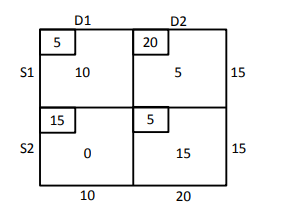
\includegraphics[width=0.75\columnwidth]{chapters/10/7/2/4/figs/fig.png}
 \end{center}
\caption{}
\label{fig:10/7/2/4Fig1}
\end{figure}
\fi

\item Find the position vector of the mid point of the vector joining the points $\vec{P}$(2, 3, 4)
and $\vec{Q}$(4, 1, –2).
\\
\solution
		\begin{enumerate}[label=\thesubsection.\arabic*,ref=\thesubsection.\theenumi]
\item Find the coordinates of the point which divides the join of $(-1,7) $ and $ (4,-3)$ in the ratio 2:3.
	\\
		\solution
	\input{chapters/10/7/2/1/section.tex}
\item Find the coordinates of the point $\vec{R}$ on the line segment joining the points $\vec{P}(-1,3)$ and $\vec{Q}(2,5)$ such that $PR=\frac{3}{5}PQ$.
\item Find the ratio in which the point $\vec{P}\brak{\frac{3}{4},\frac{5}{12}}$ divides the line segment joining the points $\vec{A}\brak{\frac{1}{2},\frac{3}{2}}$ and $ \vec{B}(2,-5)$.
\item Find the coordinates of the point which divides the line segment joining the points $(4,-3)$ and $(8,5)$ in the ratio $3:1$ internally.
\item Find the coordinates of the point $\vec{P}$ on $AD$ such that $AP : PD = 2 : 1$.
\item If the point $\vec{P} (2, 1)$ lies on the line segment joining points $\vec{A} (4, 2)$  and $ \vec{B} (8, 4)$,
then
\begin{enumerate}
	\item $AP =\frac{1}{3}{AB}$ 
\item ${AP}={PE}$
\item ${PB}=\frac{1}{3}{AB}$
\item${AP}=\frac{1}{2}{AB}$
 \end{enumerate}
\item Find the ratio in which the line segment joining the points $(-3,10)$  and  $(6,-8)$  is divided by $ (-1,6)$.
	\\
		\solution
	\input{chapters/10/7/2/4/section.tex}
\item Find the position vector of the mid point of the vector joining the points $\vec{P}$(2, 3, 4)
and $\vec{Q}$(4, 1, –2).
\\
\solution
		\input{chapters/12/10/2/16/section.tex}
\item Let $\vec{A}(4, 2), \vec{B}(6, 5)$  and $ \vec{C}(1, 4)$ be the vertices of $\triangle ABC$.
\begin{enumerate}
\item If $\vec{A}$ and  $\vec{B}$ are $(-2,-2)$ and  $(2,-4)$, respectively, find the coordinates of $\vec{P}$ such that $AP= \frac {3}{7}AB$  and $ \vec{P}$ lies on the line segment $AB$.
	\\
		\solution
	\input{chapters/10/7/2/8/section.tex}
\item Find the coordinates of the points which divide the line segment joining $A(-2,2)$  and  $\vec{B}(2,8)$ into four equal parts.
	\\
		\solution
	\input{chapters/10/7/2/9/section.tex}
\item In what ratio does the point $(-4,6)$ divide the line segment joining the points $\vec{A}(-6,0)$ and $\vec{B}(3,-8)$?
\item Given that $\vec{P}(3,2,-4), \vec{Q}(5,4,-6)$ and $\vec{R}(9,8,-10)$ are collinear. Find the ratio in which $\vec{Q}$ divides $PR$.
\item Points $\vec{A}(-6,10),\vec{B}(-4,6)$  and  $\vec{C}(3,-8)$ are collinear such that $AB=  \frac{2}{9}AC$.
\item The point which divides the line segment joining the points $\vec{P} (7, –6) $  and  $\vec{Q}(3, 4)$ in the 
ratio 1 : 2 internally lies in  which quadrant?
\item Find the coordinates of the points of trisection of the line segment joining $(4,-1)$  and  $(-2,3)$.
	\\
		\solution
	\input{chapters/10/7/2/2/section.tex}
\item Find the coordinates of the points which trisect the line segment joining the points $\vec{P}(4,2,-6)$ and $\vec{Q}(10,-16,6)$.
\item Find the coordinates of the points of trisection (i.e. points dividing to three equal parts) of the line segment joining the points $\vec{A}(2,-2)$ and $\vec{B}(-7,4)$.
\item Point $\vec{P}(5,-3)$ is one of the two points of trisection of line segment joining the points $\vec{A}(7,-2)$ and $\vec{B}(1,-5)$
\item Find the position vector of a point $\vec{R}$ which divides the line joining two points $\vec{P}$
and $\vec{Q}$ whose position vectors are $\hat{i}+2\hat{j}-\hat{k}$ and $-\hat{i}+\hat{j}+\hat{k}$ respectively, in the
ratio 2 : 1
\begin{enumerate}
    \item  internally
    \item  externally
\end{enumerate}
%\solution
%		\input{chapters/12/10/2/15/section.tex}
\item Find the coordinates of the point which divides the line segment joining the points which divides the line segment joining  the points $(-2,3,5)$ and $(1,-4,6)$ in the ratio 
\begin{enumerate}
\item $2:3$ internally,
\item $2:3$ externally
\end{enumerate}
\item Find the coordinates of the point which divides the line segment joining the points $(1,-2,3)$ and $(3,4,-5)$ in the ratio $2:3$
\begin{enumerate}
\item internally, and
\item externally
\end{enumerate}
\item Consider two points $\vec{P}$ and $\vec{Q}$ with position vectors $\overrightarrow{OP} = 3\overrightarrow{a}-2\overrightarrow{b}$ and $\overrightarrow{OQ}=\overrightarrow{a}+\overrightarrow{b}$. Find the position vector of a point $\vec{R}$ which divides the line joining $\vec{P}$ and $\vec{Q}$ in the ratio $2:1$, 
\begin{enumerate}
\item internally, and 
\item externally.
\end{enumerate}
\item The median from $\vec{A}$ meets $BC$ at $\vec{D}$. Find the coordinates of the point $\vec{D}$.
\item Find the coordinates of points $\vec{Q}$ and $\vec{R}$ on medians $BE$ and $CF$ respectively such that $BQ : QE = 2 : 1$  and  $CR : RF = 2 : 1$.
\item What do you observe?
\item If $\vec{A}, \vec{B}$ and $\vec{C}$  are the vertices of $\triangle ABC$, find the coordinates of the centroid of the triangle.
\end{enumerate}
\solution
	\input{chapters/10/7/4/7/section.tex}
\item If $\vec{P}(9a-2,-b)$ divides line segment joining $\vec{A}(3a+1,-3)$ and $\vec{B}(8a,5)$ in the ratio 3:1, find the values of $a$ and $b$.
\item Find the position vector of a point $\vec{R}$ which divides the line joining two points $\vec{P}$ and $\vec{Q}$ whose position vectors are $2\vec{a}+\vec{b}$ and $\vec{a}-3\vec{b}$ externally in the ratio $1:2$.
\item The position vector of the point which divides the join of points 2$\vec{a}$-3$\vec{b}$ $\text{and}$ $\vec{a}+\vec{b}$ in the ratio 3:1 is \rule{1cm}{0.1pt}.
\item If $\vec{a}$ and $\vec{b}$ are the postion vectors of $\vec{A}$ and $\vec{B}$, respectively, find the position vector of a point $\vec{C}$ in $BA$ produced such that $BC=1.5BA$.
\item Find the position vector of a point $\vec{R}$ which divides the line joining two points $\vec{P}$ and $\vec{Q}$ whose position vectors are $(2\vec{a}+\vec{b})$ and $(\vec{a}-3\vec{b})$
externally in the ratio 1 : 2. Also, show that $\vec{P}$ is the mid point of the line segment $RQ$.
\end{enumerate}

\item Let $\vec{A}(4, 2), \vec{B}(6, 5)$  and $ \vec{C}(1, 4)$ be the vertices of $\triangle ABC$.
\begin{enumerate}
\item If $\vec{A}$ and  $\vec{B}$ are $(-2,-2)$ and  $(2,-4)$, respectively, find the coordinates of $\vec{P}$ such that $AP= \frac {3}{7}AB$  and $ \vec{P}$ lies on the line segment $AB$.
	\\
		\solution
	\begin{enumerate}[label=\thesubsection.\arabic*,ref=\thesubsection.\theenumi]
\item Find the coordinates of the point which divides the join of $(-1,7) $ and $ (4,-3)$ in the ratio 2:3.
	\\
		\solution
	\input{chapters/10/7/2/1/section.tex}
\item Find the coordinates of the point $\vec{R}$ on the line segment joining the points $\vec{P}(-1,3)$ and $\vec{Q}(2,5)$ such that $PR=\frac{3}{5}PQ$.
\item Find the ratio in which the point $\vec{P}\brak{\frac{3}{4},\frac{5}{12}}$ divides the line segment joining the points $\vec{A}\brak{\frac{1}{2},\frac{3}{2}}$ and $ \vec{B}(2,-5)$.
\item Find the coordinates of the point which divides the line segment joining the points $(4,-3)$ and $(8,5)$ in the ratio $3:1$ internally.
\item Find the coordinates of the point $\vec{P}$ on $AD$ such that $AP : PD = 2 : 1$.
\item If the point $\vec{P} (2, 1)$ lies on the line segment joining points $\vec{A} (4, 2)$  and $ \vec{B} (8, 4)$,
then
\begin{enumerate}
	\item $AP =\frac{1}{3}{AB}$ 
\item ${AP}={PE}$
\item ${PB}=\frac{1}{3}{AB}$
\item${AP}=\frac{1}{2}{AB}$
 \end{enumerate}
\item Find the ratio in which the line segment joining the points $(-3,10)$  and  $(6,-8)$  is divided by $ (-1,6)$.
	\\
		\solution
	\input{chapters/10/7/2/4/section.tex}
\item Find the position vector of the mid point of the vector joining the points $\vec{P}$(2, 3, 4)
and $\vec{Q}$(4, 1, –2).
\\
\solution
		\input{chapters/12/10/2/16/section.tex}
\item Let $\vec{A}(4, 2), \vec{B}(6, 5)$  and $ \vec{C}(1, 4)$ be the vertices of $\triangle ABC$.
\begin{enumerate}
\item If $\vec{A}$ and  $\vec{B}$ are $(-2,-2)$ and  $(2,-4)$, respectively, find the coordinates of $\vec{P}$ such that $AP= \frac {3}{7}AB$  and $ \vec{P}$ lies on the line segment $AB$.
	\\
		\solution
	\input{chapters/10/7/2/8/section.tex}
\item Find the coordinates of the points which divide the line segment joining $A(-2,2)$  and  $\vec{B}(2,8)$ into four equal parts.
	\\
		\solution
	\input{chapters/10/7/2/9/section.tex}
\item In what ratio does the point $(-4,6)$ divide the line segment joining the points $\vec{A}(-6,0)$ and $\vec{B}(3,-8)$?
\item Given that $\vec{P}(3,2,-4), \vec{Q}(5,4,-6)$ and $\vec{R}(9,8,-10)$ are collinear. Find the ratio in which $\vec{Q}$ divides $PR$.
\item Points $\vec{A}(-6,10),\vec{B}(-4,6)$  and  $\vec{C}(3,-8)$ are collinear such that $AB=  \frac{2}{9}AC$.
\item The point which divides the line segment joining the points $\vec{P} (7, –6) $  and  $\vec{Q}(3, 4)$ in the 
ratio 1 : 2 internally lies in  which quadrant?
\item Find the coordinates of the points of trisection of the line segment joining $(4,-1)$  and  $(-2,3)$.
	\\
		\solution
	\input{chapters/10/7/2/2/section.tex}
\item Find the coordinates of the points which trisect the line segment joining the points $\vec{P}(4,2,-6)$ and $\vec{Q}(10,-16,6)$.
\item Find the coordinates of the points of trisection (i.e. points dividing to three equal parts) of the line segment joining the points $\vec{A}(2,-2)$ and $\vec{B}(-7,4)$.
\item Point $\vec{P}(5,-3)$ is one of the two points of trisection of line segment joining the points $\vec{A}(7,-2)$ and $\vec{B}(1,-5)$
\item Find the position vector of a point $\vec{R}$ which divides the line joining two points $\vec{P}$
and $\vec{Q}$ whose position vectors are $\hat{i}+2\hat{j}-\hat{k}$ and $-\hat{i}+\hat{j}+\hat{k}$ respectively, in the
ratio 2 : 1
\begin{enumerate}
    \item  internally
    \item  externally
\end{enumerate}
%\solution
%		\input{chapters/12/10/2/15/section.tex}
\item Find the coordinates of the point which divides the line segment joining the points which divides the line segment joining  the points $(-2,3,5)$ and $(1,-4,6)$ in the ratio 
\begin{enumerate}
\item $2:3$ internally,
\item $2:3$ externally
\end{enumerate}
\item Find the coordinates of the point which divides the line segment joining the points $(1,-2,3)$ and $(3,4,-5)$ in the ratio $2:3$
\begin{enumerate}
\item internally, and
\item externally
\end{enumerate}
\item Consider two points $\vec{P}$ and $\vec{Q}$ with position vectors $\overrightarrow{OP} = 3\overrightarrow{a}-2\overrightarrow{b}$ and $\overrightarrow{OQ}=\overrightarrow{a}+\overrightarrow{b}$. Find the position vector of a point $\vec{R}$ which divides the line joining $\vec{P}$ and $\vec{Q}$ in the ratio $2:1$, 
\begin{enumerate}
\item internally, and 
\item externally.
\end{enumerate}
\item The median from $\vec{A}$ meets $BC$ at $\vec{D}$. Find the coordinates of the point $\vec{D}$.
\item Find the coordinates of points $\vec{Q}$ and $\vec{R}$ on medians $BE$ and $CF$ respectively such that $BQ : QE = 2 : 1$  and  $CR : RF = 2 : 1$.
\item What do you observe?
\item If $\vec{A}, \vec{B}$ and $\vec{C}$  are the vertices of $\triangle ABC$, find the coordinates of the centroid of the triangle.
\end{enumerate}
\solution
	\input{chapters/10/7/4/7/section.tex}
\item If $\vec{P}(9a-2,-b)$ divides line segment joining $\vec{A}(3a+1,-3)$ and $\vec{B}(8a,5)$ in the ratio 3:1, find the values of $a$ and $b$.
\item Find the position vector of a point $\vec{R}$ which divides the line joining two points $\vec{P}$ and $\vec{Q}$ whose position vectors are $2\vec{a}+\vec{b}$ and $\vec{a}-3\vec{b}$ externally in the ratio $1:2$.
\item The position vector of the point which divides the join of points 2$\vec{a}$-3$\vec{b}$ $\text{and}$ $\vec{a}+\vec{b}$ in the ratio 3:1 is \rule{1cm}{0.1pt}.
\item If $\vec{a}$ and $\vec{b}$ are the postion vectors of $\vec{A}$ and $\vec{B}$, respectively, find the position vector of a point $\vec{C}$ in $BA$ produced such that $BC=1.5BA$.
\item Find the position vector of a point $\vec{R}$ which divides the line joining two points $\vec{P}$ and $\vec{Q}$ whose position vectors are $(2\vec{a}+\vec{b})$ and $(\vec{a}-3\vec{b})$
externally in the ratio 1 : 2. Also, show that $\vec{P}$ is the mid point of the line segment $RQ$.
\end{enumerate}

\item Find the coordinates of the points which divide the line segment joining $A(-2,2)$  and  $\vec{B}(2,8)$ into four equal parts.
	\\
		\solution
	\begin{enumerate}[label=\thesubsection.\arabic*,ref=\thesubsection.\theenumi]
\item Find the coordinates of the point which divides the join of $(-1,7) $ and $ (4,-3)$ in the ratio 2:3.
	\\
		\solution
	\input{chapters/10/7/2/1/section.tex}
\item Find the coordinates of the point $\vec{R}$ on the line segment joining the points $\vec{P}(-1,3)$ and $\vec{Q}(2,5)$ such that $PR=\frac{3}{5}PQ$.
\item Find the ratio in which the point $\vec{P}\brak{\frac{3}{4},\frac{5}{12}}$ divides the line segment joining the points $\vec{A}\brak{\frac{1}{2},\frac{3}{2}}$ and $ \vec{B}(2,-5)$.
\item Find the coordinates of the point which divides the line segment joining the points $(4,-3)$ and $(8,5)$ in the ratio $3:1$ internally.
\item Find the coordinates of the point $\vec{P}$ on $AD$ such that $AP : PD = 2 : 1$.
\item If the point $\vec{P} (2, 1)$ lies on the line segment joining points $\vec{A} (4, 2)$  and $ \vec{B} (8, 4)$,
then
\begin{enumerate}
	\item $AP =\frac{1}{3}{AB}$ 
\item ${AP}={PE}$
\item ${PB}=\frac{1}{3}{AB}$
\item${AP}=\frac{1}{2}{AB}$
 \end{enumerate}
\item Find the ratio in which the line segment joining the points $(-3,10)$  and  $(6,-8)$  is divided by $ (-1,6)$.
	\\
		\solution
	\input{chapters/10/7/2/4/section.tex}
\item Find the position vector of the mid point of the vector joining the points $\vec{P}$(2, 3, 4)
and $\vec{Q}$(4, 1, –2).
\\
\solution
		\input{chapters/12/10/2/16/section.tex}
\item Let $\vec{A}(4, 2), \vec{B}(6, 5)$  and $ \vec{C}(1, 4)$ be the vertices of $\triangle ABC$.
\begin{enumerate}
\item If $\vec{A}$ and  $\vec{B}$ are $(-2,-2)$ and  $(2,-4)$, respectively, find the coordinates of $\vec{P}$ such that $AP= \frac {3}{7}AB$  and $ \vec{P}$ lies on the line segment $AB$.
	\\
		\solution
	\input{chapters/10/7/2/8/section.tex}
\item Find the coordinates of the points which divide the line segment joining $A(-2,2)$  and  $\vec{B}(2,8)$ into four equal parts.
	\\
		\solution
	\input{chapters/10/7/2/9/section.tex}
\item In what ratio does the point $(-4,6)$ divide the line segment joining the points $\vec{A}(-6,0)$ and $\vec{B}(3,-8)$?
\item Given that $\vec{P}(3,2,-4), \vec{Q}(5,4,-6)$ and $\vec{R}(9,8,-10)$ are collinear. Find the ratio in which $\vec{Q}$ divides $PR$.
\item Points $\vec{A}(-6,10),\vec{B}(-4,6)$  and  $\vec{C}(3,-8)$ are collinear such that $AB=  \frac{2}{9}AC$.
\item The point which divides the line segment joining the points $\vec{P} (7, –6) $  and  $\vec{Q}(3, 4)$ in the 
ratio 1 : 2 internally lies in  which quadrant?
\item Find the coordinates of the points of trisection of the line segment joining $(4,-1)$  and  $(-2,3)$.
	\\
		\solution
	\input{chapters/10/7/2/2/section.tex}
\item Find the coordinates of the points which trisect the line segment joining the points $\vec{P}(4,2,-6)$ and $\vec{Q}(10,-16,6)$.
\item Find the coordinates of the points of trisection (i.e. points dividing to three equal parts) of the line segment joining the points $\vec{A}(2,-2)$ and $\vec{B}(-7,4)$.
\item Point $\vec{P}(5,-3)$ is one of the two points of trisection of line segment joining the points $\vec{A}(7,-2)$ and $\vec{B}(1,-5)$
\item Find the position vector of a point $\vec{R}$ which divides the line joining two points $\vec{P}$
and $\vec{Q}$ whose position vectors are $\hat{i}+2\hat{j}-\hat{k}$ and $-\hat{i}+\hat{j}+\hat{k}$ respectively, in the
ratio 2 : 1
\begin{enumerate}
    \item  internally
    \item  externally
\end{enumerate}
%\solution
%		\input{chapters/12/10/2/15/section.tex}
\item Find the coordinates of the point which divides the line segment joining the points which divides the line segment joining  the points $(-2,3,5)$ and $(1,-4,6)$ in the ratio 
\begin{enumerate}
\item $2:3$ internally,
\item $2:3$ externally
\end{enumerate}
\item Find the coordinates of the point which divides the line segment joining the points $(1,-2,3)$ and $(3,4,-5)$ in the ratio $2:3$
\begin{enumerate}
\item internally, and
\item externally
\end{enumerate}
\item Consider two points $\vec{P}$ and $\vec{Q}$ with position vectors $\overrightarrow{OP} = 3\overrightarrow{a}-2\overrightarrow{b}$ and $\overrightarrow{OQ}=\overrightarrow{a}+\overrightarrow{b}$. Find the position vector of a point $\vec{R}$ which divides the line joining $\vec{P}$ and $\vec{Q}$ in the ratio $2:1$, 
\begin{enumerate}
\item internally, and 
\item externally.
\end{enumerate}
\item The median from $\vec{A}$ meets $BC$ at $\vec{D}$. Find the coordinates of the point $\vec{D}$.
\item Find the coordinates of points $\vec{Q}$ and $\vec{R}$ on medians $BE$ and $CF$ respectively such that $BQ : QE = 2 : 1$  and  $CR : RF = 2 : 1$.
\item What do you observe?
\item If $\vec{A}, \vec{B}$ and $\vec{C}$  are the vertices of $\triangle ABC$, find the coordinates of the centroid of the triangle.
\end{enumerate}
\solution
	\input{chapters/10/7/4/7/section.tex}
\item If $\vec{P}(9a-2,-b)$ divides line segment joining $\vec{A}(3a+1,-3)$ and $\vec{B}(8a,5)$ in the ratio 3:1, find the values of $a$ and $b$.
\item Find the position vector of a point $\vec{R}$ which divides the line joining two points $\vec{P}$ and $\vec{Q}$ whose position vectors are $2\vec{a}+\vec{b}$ and $\vec{a}-3\vec{b}$ externally in the ratio $1:2$.
\item The position vector of the point which divides the join of points 2$\vec{a}$-3$\vec{b}$ $\text{and}$ $\vec{a}+\vec{b}$ in the ratio 3:1 is \rule{1cm}{0.1pt}.
\item If $\vec{a}$ and $\vec{b}$ are the postion vectors of $\vec{A}$ and $\vec{B}$, respectively, find the position vector of a point $\vec{C}$ in $BA$ produced such that $BC=1.5BA$.
\item Find the position vector of a point $\vec{R}$ which divides the line joining two points $\vec{P}$ and $\vec{Q}$ whose position vectors are $(2\vec{a}+\vec{b})$ and $(\vec{a}-3\vec{b})$
externally in the ratio 1 : 2. Also, show that $\vec{P}$ is the mid point of the line segment $RQ$.
\end{enumerate}

\item In what ratio does the point $(-4,6)$ divide the line segment joining the points $\vec{A}(-6,0)$ and $\vec{B}(3,-8)$?
\item Given that $\vec{P}(3,2,-4), \vec{Q}(5,4,-6)$ and $\vec{R}(9,8,-10)$ are collinear. Find the ratio in which $\vec{Q}$ divides $PR$.
\item Points $\vec{A}(-6,10),\vec{B}(-4,6)$  and  $\vec{C}(3,-8)$ are collinear such that $AB=  \frac{2}{9}AC$.
\item The point which divides the line segment joining the points $\vec{P} (7, –6) $  and  $\vec{Q}(3, 4)$ in the 
ratio 1 : 2 internally lies in  which quadrant?
\item Find the coordinates of the points of trisection of the line segment joining $(4,-1)$  and  $(-2,3)$.
	\\
		\solution
	Using section formula,
\begin{align}
\vec{R}=\frac{1}{1+\frac{1}{2}}\brak{\myvec{4\\-1}+\frac{1}{2}\myvec{-2\\3}}
=\myvec{2\\ \frac{1}{3}}\\
\vec{S}=\frac{1}{1+\frac{2}{1}}\brak{\myvec{4\\-1}+\frac{2}{1}\myvec{-2\\3}}
=\myvec{0\\ \frac{5}{3}}
\end{align}
which are the desired points of trisection.
\iffalse
See
		\figref{fig:chapters/10/7/2/2/Figure}
\begin{figure}[H]
\centering
\includegraphics[width=0.75\columnwidth]{chapters/10/7/2/2/figs/dj.pdf}
\caption{}
		\label{fig:chapters/10/7/2/2/Figure}
\end{figure}
\fi

\item Find the coordinates of the points which trisect the line segment joining the points $\vec{P}(4,2,-6)$ and $\vec{Q}(10,-16,6)$.
\item Find the coordinates of the points of trisection (i.e. points dividing to three equal parts) of the line segment joining the points $\vec{A}(2,-2)$ and $\vec{B}(-7,4)$.
\item Point $\vec{P}(5,-3)$ is one of the two points of trisection of line segment joining the points $\vec{A}(7,-2)$ and $\vec{B}(1,-5)$
\item Find the position vector of a point $\vec{R}$ which divides the line joining two points $\vec{P}$
and $\vec{Q}$ whose position vectors are $\hat{i}+2\hat{j}-\hat{k}$ and $-\hat{i}+\hat{j}+\hat{k}$ respectively, in the
ratio 2 : 1
\begin{enumerate}
    \item  internally
    \item  externally
\end{enumerate}
%\solution
%		\begin{enumerate}[label=\thesubsection.\arabic*,ref=\thesubsection.\theenumi]
\item Find the coordinates of the point which divides the join of $(-1,7) $ and $ (4,-3)$ in the ratio 2:3.
	\\
		\solution
	\input{chapters/10/7/2/1/section.tex}
\item Find the coordinates of the point $\vec{R}$ on the line segment joining the points $\vec{P}(-1,3)$ and $\vec{Q}(2,5)$ such that $PR=\frac{3}{5}PQ$.
\item Find the ratio in which the point $\vec{P}\brak{\frac{3}{4},\frac{5}{12}}$ divides the line segment joining the points $\vec{A}\brak{\frac{1}{2},\frac{3}{2}}$ and $ \vec{B}(2,-5)$.
\item Find the coordinates of the point which divides the line segment joining the points $(4,-3)$ and $(8,5)$ in the ratio $3:1$ internally.
\item Find the coordinates of the point $\vec{P}$ on $AD$ such that $AP : PD = 2 : 1$.
\item If the point $\vec{P} (2, 1)$ lies on the line segment joining points $\vec{A} (4, 2)$  and $ \vec{B} (8, 4)$,
then
\begin{enumerate}
	\item $AP =\frac{1}{3}{AB}$ 
\item ${AP}={PE}$
\item ${PB}=\frac{1}{3}{AB}$
\item${AP}=\frac{1}{2}{AB}$
 \end{enumerate}
\item Find the ratio in which the line segment joining the points $(-3,10)$  and  $(6,-8)$  is divided by $ (-1,6)$.
	\\
		\solution
	\input{chapters/10/7/2/4/section.tex}
\item Find the position vector of the mid point of the vector joining the points $\vec{P}$(2, 3, 4)
and $\vec{Q}$(4, 1, –2).
\\
\solution
		\input{chapters/12/10/2/16/section.tex}
\item Let $\vec{A}(4, 2), \vec{B}(6, 5)$  and $ \vec{C}(1, 4)$ be the vertices of $\triangle ABC$.
\begin{enumerate}
\item If $\vec{A}$ and  $\vec{B}$ are $(-2,-2)$ and  $(2,-4)$, respectively, find the coordinates of $\vec{P}$ such that $AP= \frac {3}{7}AB$  and $ \vec{P}$ lies on the line segment $AB$.
	\\
		\solution
	\input{chapters/10/7/2/8/section.tex}
\item Find the coordinates of the points which divide the line segment joining $A(-2,2)$  and  $\vec{B}(2,8)$ into four equal parts.
	\\
		\solution
	\input{chapters/10/7/2/9/section.tex}
\item In what ratio does the point $(-4,6)$ divide the line segment joining the points $\vec{A}(-6,0)$ and $\vec{B}(3,-8)$?
\item Given that $\vec{P}(3,2,-4), \vec{Q}(5,4,-6)$ and $\vec{R}(9,8,-10)$ are collinear. Find the ratio in which $\vec{Q}$ divides $PR$.
\item Points $\vec{A}(-6,10),\vec{B}(-4,6)$  and  $\vec{C}(3,-8)$ are collinear such that $AB=  \frac{2}{9}AC$.
\item The point which divides the line segment joining the points $\vec{P} (7, –6) $  and  $\vec{Q}(3, 4)$ in the 
ratio 1 : 2 internally lies in  which quadrant?
\item Find the coordinates of the points of trisection of the line segment joining $(4,-1)$  and  $(-2,3)$.
	\\
		\solution
	\input{chapters/10/7/2/2/section.tex}
\item Find the coordinates of the points which trisect the line segment joining the points $\vec{P}(4,2,-6)$ and $\vec{Q}(10,-16,6)$.
\item Find the coordinates of the points of trisection (i.e. points dividing to three equal parts) of the line segment joining the points $\vec{A}(2,-2)$ and $\vec{B}(-7,4)$.
\item Point $\vec{P}(5,-3)$ is one of the two points of trisection of line segment joining the points $\vec{A}(7,-2)$ and $\vec{B}(1,-5)$
\item Find the position vector of a point $\vec{R}$ which divides the line joining two points $\vec{P}$
and $\vec{Q}$ whose position vectors are $\hat{i}+2\hat{j}-\hat{k}$ and $-\hat{i}+\hat{j}+\hat{k}$ respectively, in the
ratio 2 : 1
\begin{enumerate}
    \item  internally
    \item  externally
\end{enumerate}
%\solution
%		\input{chapters/12/10/2/15/section.tex}
\item Find the coordinates of the point which divides the line segment joining the points which divides the line segment joining  the points $(-2,3,5)$ and $(1,-4,6)$ in the ratio 
\begin{enumerate}
\item $2:3$ internally,
\item $2:3$ externally
\end{enumerate}
\item Find the coordinates of the point which divides the line segment joining the points $(1,-2,3)$ and $(3,4,-5)$ in the ratio $2:3$
\begin{enumerate}
\item internally, and
\item externally
\end{enumerate}
\item Consider two points $\vec{P}$ and $\vec{Q}$ with position vectors $\overrightarrow{OP} = 3\overrightarrow{a}-2\overrightarrow{b}$ and $\overrightarrow{OQ}=\overrightarrow{a}+\overrightarrow{b}$. Find the position vector of a point $\vec{R}$ which divides the line joining $\vec{P}$ and $\vec{Q}$ in the ratio $2:1$, 
\begin{enumerate}
\item internally, and 
\item externally.
\end{enumerate}
\item The median from $\vec{A}$ meets $BC$ at $\vec{D}$. Find the coordinates of the point $\vec{D}$.
\item Find the coordinates of points $\vec{Q}$ and $\vec{R}$ on medians $BE$ and $CF$ respectively such that $BQ : QE = 2 : 1$  and  $CR : RF = 2 : 1$.
\item What do you observe?
\item If $\vec{A}, \vec{B}$ and $\vec{C}$  are the vertices of $\triangle ABC$, find the coordinates of the centroid of the triangle.
\end{enumerate}
\solution
	\input{chapters/10/7/4/7/section.tex}
\item If $\vec{P}(9a-2,-b)$ divides line segment joining $\vec{A}(3a+1,-3)$ and $\vec{B}(8a,5)$ in the ratio 3:1, find the values of $a$ and $b$.
\item Find the position vector of a point $\vec{R}$ which divides the line joining two points $\vec{P}$ and $\vec{Q}$ whose position vectors are $2\vec{a}+\vec{b}$ and $\vec{a}-3\vec{b}$ externally in the ratio $1:2$.
\item The position vector of the point which divides the join of points 2$\vec{a}$-3$\vec{b}$ $\text{and}$ $\vec{a}+\vec{b}$ in the ratio 3:1 is \rule{1cm}{0.1pt}.
\item If $\vec{a}$ and $\vec{b}$ are the postion vectors of $\vec{A}$ and $\vec{B}$, respectively, find the position vector of a point $\vec{C}$ in $BA$ produced such that $BC=1.5BA$.
\item Find the position vector of a point $\vec{R}$ which divides the line joining two points $\vec{P}$ and $\vec{Q}$ whose position vectors are $(2\vec{a}+\vec{b})$ and $(\vec{a}-3\vec{b})$
externally in the ratio 1 : 2. Also, show that $\vec{P}$ is the mid point of the line segment $RQ$.
\end{enumerate}

\item Find the coordinates of the point which divides the line segment joining the points which divides the line segment joining  the points $(-2,3,5)$ and $(1,-4,6)$ in the ratio 
\begin{enumerate}
\item $2:3$ internally,
\item $2:3$ externally
\end{enumerate}
\item Find the coordinates of the point which divides the line segment joining the points $(1,-2,3)$ and $(3,4,-5)$ in the ratio $2:3$
\begin{enumerate}
\item internally, and
\item externally
\end{enumerate}
\item Consider two points $\vec{P}$ and $\vec{Q}$ with position vectors $\overrightarrow{OP} = 3\overrightarrow{a}-2\overrightarrow{b}$ and $\overrightarrow{OQ}=\overrightarrow{a}+\overrightarrow{b}$. Find the position vector of a point $\vec{R}$ which divides the line joining $\vec{P}$ and $\vec{Q}$ in the ratio $2:1$, 
\begin{enumerate}
\item internally, and 
\item externally.
\end{enumerate}
\item The median from $\vec{A}$ meets $BC$ at $\vec{D}$. Find the coordinates of the point $\vec{D}$.
\item Find the coordinates of points $\vec{Q}$ and $\vec{R}$ on medians $BE$ and $CF$ respectively such that $BQ : QE = 2 : 1$  and  $CR : RF = 2 : 1$.
\item What do you observe?
\item If $\vec{A}, \vec{B}$ and $\vec{C}$  are the vertices of $\triangle ABC$, find the coordinates of the centroid of the triangle.
\end{enumerate}
\solution
	\begin{enumerate}[label=\thesubsection.\arabic*,ref=\thesubsection.\theenumi]
\item Find the coordinates of the point which divides the join of $(-1,7) $ and $ (4,-3)$ in the ratio 2:3.
	\\
		\solution
	\input{chapters/10/7/2/1/section.tex}
\item Find the coordinates of the point $\vec{R}$ on the line segment joining the points $\vec{P}(-1,3)$ and $\vec{Q}(2,5)$ such that $PR=\frac{3}{5}PQ$.
\item Find the ratio in which the point $\vec{P}\brak{\frac{3}{4},\frac{5}{12}}$ divides the line segment joining the points $\vec{A}\brak{\frac{1}{2},\frac{3}{2}}$ and $ \vec{B}(2,-5)$.
\item Find the coordinates of the point which divides the line segment joining the points $(4,-3)$ and $(8,5)$ in the ratio $3:1$ internally.
\item Find the coordinates of the point $\vec{P}$ on $AD$ such that $AP : PD = 2 : 1$.
\item If the point $\vec{P} (2, 1)$ lies on the line segment joining points $\vec{A} (4, 2)$  and $ \vec{B} (8, 4)$,
then
\begin{enumerate}
	\item $AP =\frac{1}{3}{AB}$ 
\item ${AP}={PE}$
\item ${PB}=\frac{1}{3}{AB}$
\item${AP}=\frac{1}{2}{AB}$
 \end{enumerate}
\item Find the ratio in which the line segment joining the points $(-3,10)$  and  $(6,-8)$  is divided by $ (-1,6)$.
	\\
		\solution
	\input{chapters/10/7/2/4/section.tex}
\item Find the position vector of the mid point of the vector joining the points $\vec{P}$(2, 3, 4)
and $\vec{Q}$(4, 1, –2).
\\
\solution
		\input{chapters/12/10/2/16/section.tex}
\item Let $\vec{A}(4, 2), \vec{B}(6, 5)$  and $ \vec{C}(1, 4)$ be the vertices of $\triangle ABC$.
\begin{enumerate}
\item If $\vec{A}$ and  $\vec{B}$ are $(-2,-2)$ and  $(2,-4)$, respectively, find the coordinates of $\vec{P}$ such that $AP= \frac {3}{7}AB$  and $ \vec{P}$ lies on the line segment $AB$.
	\\
		\solution
	\input{chapters/10/7/2/8/section.tex}
\item Find the coordinates of the points which divide the line segment joining $A(-2,2)$  and  $\vec{B}(2,8)$ into four equal parts.
	\\
		\solution
	\input{chapters/10/7/2/9/section.tex}
\item In what ratio does the point $(-4,6)$ divide the line segment joining the points $\vec{A}(-6,0)$ and $\vec{B}(3,-8)$?
\item Given that $\vec{P}(3,2,-4), \vec{Q}(5,4,-6)$ and $\vec{R}(9,8,-10)$ are collinear. Find the ratio in which $\vec{Q}$ divides $PR$.
\item Points $\vec{A}(-6,10),\vec{B}(-4,6)$  and  $\vec{C}(3,-8)$ are collinear such that $AB=  \frac{2}{9}AC$.
\item The point which divides the line segment joining the points $\vec{P} (7, –6) $  and  $\vec{Q}(3, 4)$ in the 
ratio 1 : 2 internally lies in  which quadrant?
\item Find the coordinates of the points of trisection of the line segment joining $(4,-1)$  and  $(-2,3)$.
	\\
		\solution
	\input{chapters/10/7/2/2/section.tex}
\item Find the coordinates of the points which trisect the line segment joining the points $\vec{P}(4,2,-6)$ and $\vec{Q}(10,-16,6)$.
\item Find the coordinates of the points of trisection (i.e. points dividing to three equal parts) of the line segment joining the points $\vec{A}(2,-2)$ and $\vec{B}(-7,4)$.
\item Point $\vec{P}(5,-3)$ is one of the two points of trisection of line segment joining the points $\vec{A}(7,-2)$ and $\vec{B}(1,-5)$
\item Find the position vector of a point $\vec{R}$ which divides the line joining two points $\vec{P}$
and $\vec{Q}$ whose position vectors are $\hat{i}+2\hat{j}-\hat{k}$ and $-\hat{i}+\hat{j}+\hat{k}$ respectively, in the
ratio 2 : 1
\begin{enumerate}
    \item  internally
    \item  externally
\end{enumerate}
%\solution
%		\input{chapters/12/10/2/15/section.tex}
\item Find the coordinates of the point which divides the line segment joining the points which divides the line segment joining  the points $(-2,3,5)$ and $(1,-4,6)$ in the ratio 
\begin{enumerate}
\item $2:3$ internally,
\item $2:3$ externally
\end{enumerate}
\item Find the coordinates of the point which divides the line segment joining the points $(1,-2,3)$ and $(3,4,-5)$ in the ratio $2:3$
\begin{enumerate}
\item internally, and
\item externally
\end{enumerate}
\item Consider two points $\vec{P}$ and $\vec{Q}$ with position vectors $\overrightarrow{OP} = 3\overrightarrow{a}-2\overrightarrow{b}$ and $\overrightarrow{OQ}=\overrightarrow{a}+\overrightarrow{b}$. Find the position vector of a point $\vec{R}$ which divides the line joining $\vec{P}$ and $\vec{Q}$ in the ratio $2:1$, 
\begin{enumerate}
\item internally, and 
\item externally.
\end{enumerate}
\item The median from $\vec{A}$ meets $BC$ at $\vec{D}$. Find the coordinates of the point $\vec{D}$.
\item Find the coordinates of points $\vec{Q}$ and $\vec{R}$ on medians $BE$ and $CF$ respectively such that $BQ : QE = 2 : 1$  and  $CR : RF = 2 : 1$.
\item What do you observe?
\item If $\vec{A}, \vec{B}$ and $\vec{C}$  are the vertices of $\triangle ABC$, find the coordinates of the centroid of the triangle.
\end{enumerate}
\solution
	\input{chapters/10/7/4/7/section.tex}
\item If $\vec{P}(9a-2,-b)$ divides line segment joining $\vec{A}(3a+1,-3)$ and $\vec{B}(8a,5)$ in the ratio 3:1, find the values of $a$ and $b$.
\item Find the position vector of a point $\vec{R}$ which divides the line joining two points $\vec{P}$ and $\vec{Q}$ whose position vectors are $2\vec{a}+\vec{b}$ and $\vec{a}-3\vec{b}$ externally in the ratio $1:2$.
\item The position vector of the point which divides the join of points 2$\vec{a}$-3$\vec{b}$ $\text{and}$ $\vec{a}+\vec{b}$ in the ratio 3:1 is \rule{1cm}{0.1pt}.
\item If $\vec{a}$ and $\vec{b}$ are the postion vectors of $\vec{A}$ and $\vec{B}$, respectively, find the position vector of a point $\vec{C}$ in $BA$ produced such that $BC=1.5BA$.
\item Find the position vector of a point $\vec{R}$ which divides the line joining two points $\vec{P}$ and $\vec{Q}$ whose position vectors are $(2\vec{a}+\vec{b})$ and $(\vec{a}-3\vec{b})$
externally in the ratio 1 : 2. Also, show that $\vec{P}$ is the mid point of the line segment $RQ$.
\end{enumerate}

\item If $\vec{P}(9a-2,-b)$ divides line segment joining $\vec{A}(3a+1,-3)$ and $\vec{B}(8a,5)$ in the ratio 3:1, find the values of $a$ and $b$.
\item Find the position vector of a point $\vec{R}$ which divides the line joining two points $\vec{P}$ and $\vec{Q}$ whose position vectors are $2\vec{a}+\vec{b}$ and $\vec{a}-3\vec{b}$ externally in the ratio $1:2$.
\item The position vector of the point which divides the join of points 2$\vec{a}$-3$\vec{b}$ $\text{and}$ $\vec{a}+\vec{b}$ in the ratio 3:1 is \rule{1cm}{0.1pt}.
\item If $\vec{a}$ and $\vec{b}$ are the postion vectors of $\vec{A}$ and $\vec{B}$, respectively, find the position vector of a point $\vec{C}$ in $BA$ produced such that $BC=1.5BA$.
\item Find the position vector of a point $\vec{R}$ which divides the line joining two points $\vec{P}$ and $\vec{Q}$ whose position vectors are $(2\vec{a}+\vec{b})$ and $(\vec{a}-3\vec{b})$
externally in the ratio 1 : 2. Also, show that $\vec{P}$ is the mid point of the line segment $RQ$.
\end{enumerate}

\item In what ratio does the point $(-4,6)$ divide the line segment joining the points $\vec{A}(-6,0)$ and $\vec{B}(3,-8)$?
\item Given that $\vec{P}(3,2,-4), \vec{Q}(5,4,-6)$ and $\vec{R}(9,8,-10)$ are collinear. Find the ratio in which $\vec{Q}$ divides $PR$.
\item Points $\vec{A}(-6,10),\vec{B}(-4,6)$  and  $\vec{C}(3,-8)$ are collinear such that $AB=  \frac{2}{9}AC$.
\item The point which divides the line segment joining the points $\vec{P} (7, –6) $  and  $\vec{Q}(3, 4)$ in the 
ratio 1 : 2 internally lies in  which quadrant?
\item Find the coordinates of the points of trisection of the line segment joining $(4,-1)$  and  $(-2,3)$.
	\\
		\solution
	Using section formula,
\begin{align}
\vec{R}=\frac{1}{1+\frac{1}{2}}\brak{\myvec{4\\-1}+\frac{1}{2}\myvec{-2\\3}}
=\myvec{2\\ \frac{1}{3}}\\
\vec{S}=\frac{1}{1+\frac{2}{1}}\brak{\myvec{4\\-1}+\frac{2}{1}\myvec{-2\\3}}
=\myvec{0\\ \frac{5}{3}}
\end{align}
which are the desired points of trisection.
\iffalse
See
		\figref{fig:chapters/10/7/2/2/Figure}
\begin{figure}[H]
\centering
\includegraphics[width=0.75\columnwidth]{chapters/10/7/2/2/figs/dj.pdf}
\caption{}
		\label{fig:chapters/10/7/2/2/Figure}
\end{figure}
\fi

\item Find the coordinates of the points which trisect the line segment joining the points $\vec{P}(4,2,-6)$ and $\vec{Q}(10,-16,6)$.
\item Find the coordinates of the points of trisection (i.e. points dividing to three equal parts) of the line segment joining the points $\vec{A}(2,-2)$ and $\vec{B}(-7,4)$.
\item Point $\vec{P}(5,-3)$ is one of the two points of trisection of line segment joining the points $\vec{A}(7,-2)$ and $\vec{B}(1,-5)$
\item Find the position vector of a point $\vec{R}$ which divides the line joining two points $\vec{P}$
and $\vec{Q}$ whose position vectors are $\hat{i}+2\hat{j}-\hat{k}$ and $-\hat{i}+\hat{j}+\hat{k}$ respectively, in the
ratio 2 : 1
\begin{enumerate}
    \item  internally
    \item  externally
\end{enumerate}
%\solution
%		\begin{enumerate}[label=\thesubsection.\arabic*,ref=\thesubsection.\theenumi]
\item Find the coordinates of the point which divides the join of $(-1,7) $ and $ (4,-3)$ in the ratio 2:3.
	\\
		\solution
	\begin{enumerate}[label=\thesubsection.\arabic*,ref=\thesubsection.\theenumi]
\item Find the coordinates of the point which divides the join of $(-1,7) $ and $ (4,-3)$ in the ratio 2:3.
	\\
		\solution
	\input{chapters/10/7/2/1/section.tex}
\item Find the coordinates of the point $\vec{R}$ on the line segment joining the points $\vec{P}(-1,3)$ and $\vec{Q}(2,5)$ such that $PR=\frac{3}{5}PQ$.
\item Find the ratio in which the point $\vec{P}\brak{\frac{3}{4},\frac{5}{12}}$ divides the line segment joining the points $\vec{A}\brak{\frac{1}{2},\frac{3}{2}}$ and $ \vec{B}(2,-5)$.
\item Find the coordinates of the point which divides the line segment joining the points $(4,-3)$ and $(8,5)$ in the ratio $3:1$ internally.
\item Find the coordinates of the point $\vec{P}$ on $AD$ such that $AP : PD = 2 : 1$.
\item If the point $\vec{P} (2, 1)$ lies on the line segment joining points $\vec{A} (4, 2)$  and $ \vec{B} (8, 4)$,
then
\begin{enumerate}
	\item $AP =\frac{1}{3}{AB}$ 
\item ${AP}={PE}$
\item ${PB}=\frac{1}{3}{AB}$
\item${AP}=\frac{1}{2}{AB}$
 \end{enumerate}
\item Find the ratio in which the line segment joining the points $(-3,10)$  and  $(6,-8)$  is divided by $ (-1,6)$.
	\\
		\solution
	\input{chapters/10/7/2/4/section.tex}
\item Find the position vector of the mid point of the vector joining the points $\vec{P}$(2, 3, 4)
and $\vec{Q}$(4, 1, –2).
\\
\solution
		\input{chapters/12/10/2/16/section.tex}
\item Let $\vec{A}(4, 2), \vec{B}(6, 5)$  and $ \vec{C}(1, 4)$ be the vertices of $\triangle ABC$.
\begin{enumerate}
\item If $\vec{A}$ and  $\vec{B}$ are $(-2,-2)$ and  $(2,-4)$, respectively, find the coordinates of $\vec{P}$ such that $AP= \frac {3}{7}AB$  and $ \vec{P}$ lies on the line segment $AB$.
	\\
		\solution
	\input{chapters/10/7/2/8/section.tex}
\item Find the coordinates of the points which divide the line segment joining $A(-2,2)$  and  $\vec{B}(2,8)$ into four equal parts.
	\\
		\solution
	\input{chapters/10/7/2/9/section.tex}
\item In what ratio does the point $(-4,6)$ divide the line segment joining the points $\vec{A}(-6,0)$ and $\vec{B}(3,-8)$?
\item Given that $\vec{P}(3,2,-4), \vec{Q}(5,4,-6)$ and $\vec{R}(9,8,-10)$ are collinear. Find the ratio in which $\vec{Q}$ divides $PR$.
\item Points $\vec{A}(-6,10),\vec{B}(-4,6)$  and  $\vec{C}(3,-8)$ are collinear such that $AB=  \frac{2}{9}AC$.
\item The point which divides the line segment joining the points $\vec{P} (7, –6) $  and  $\vec{Q}(3, 4)$ in the 
ratio 1 : 2 internally lies in  which quadrant?
\item Find the coordinates of the points of trisection of the line segment joining $(4,-1)$  and  $(-2,3)$.
	\\
		\solution
	\input{chapters/10/7/2/2/section.tex}
\item Find the coordinates of the points which trisect the line segment joining the points $\vec{P}(4,2,-6)$ and $\vec{Q}(10,-16,6)$.
\item Find the coordinates of the points of trisection (i.e. points dividing to three equal parts) of the line segment joining the points $\vec{A}(2,-2)$ and $\vec{B}(-7,4)$.
\item Point $\vec{P}(5,-3)$ is one of the two points of trisection of line segment joining the points $\vec{A}(7,-2)$ and $\vec{B}(1,-5)$
\item Find the position vector of a point $\vec{R}$ which divides the line joining two points $\vec{P}$
and $\vec{Q}$ whose position vectors are $\hat{i}+2\hat{j}-\hat{k}$ and $-\hat{i}+\hat{j}+\hat{k}$ respectively, in the
ratio 2 : 1
\begin{enumerate}
    \item  internally
    \item  externally
\end{enumerate}
%\solution
%		\input{chapters/12/10/2/15/section.tex}
\item Find the coordinates of the point which divides the line segment joining the points which divides the line segment joining  the points $(-2,3,5)$ and $(1,-4,6)$ in the ratio 
\begin{enumerate}
\item $2:3$ internally,
\item $2:3$ externally
\end{enumerate}
\item Find the coordinates of the point which divides the line segment joining the points $(1,-2,3)$ and $(3,4,-5)$ in the ratio $2:3$
\begin{enumerate}
\item internally, and
\item externally
\end{enumerate}
\item Consider two points $\vec{P}$ and $\vec{Q}$ with position vectors $\overrightarrow{OP} = 3\overrightarrow{a}-2\overrightarrow{b}$ and $\overrightarrow{OQ}=\overrightarrow{a}+\overrightarrow{b}$. Find the position vector of a point $\vec{R}$ which divides the line joining $\vec{P}$ and $\vec{Q}$ in the ratio $2:1$, 
\begin{enumerate}
\item internally, and 
\item externally.
\end{enumerate}
\item The median from $\vec{A}$ meets $BC$ at $\vec{D}$. Find the coordinates of the point $\vec{D}$.
\item Find the coordinates of points $\vec{Q}$ and $\vec{R}$ on medians $BE$ and $CF$ respectively such that $BQ : QE = 2 : 1$  and  $CR : RF = 2 : 1$.
\item What do you observe?
\item If $\vec{A}, \vec{B}$ and $\vec{C}$  are the vertices of $\triangle ABC$, find the coordinates of the centroid of the triangle.
\end{enumerate}
\solution
	\input{chapters/10/7/4/7/section.tex}
\item If $\vec{P}(9a-2,-b)$ divides line segment joining $\vec{A}(3a+1,-3)$ and $\vec{B}(8a,5)$ in the ratio 3:1, find the values of $a$ and $b$.
\item Find the position vector of a point $\vec{R}$ which divides the line joining two points $\vec{P}$ and $\vec{Q}$ whose position vectors are $2\vec{a}+\vec{b}$ and $\vec{a}-3\vec{b}$ externally in the ratio $1:2$.
\item The position vector of the point which divides the join of points 2$\vec{a}$-3$\vec{b}$ $\text{and}$ $\vec{a}+\vec{b}$ in the ratio 3:1 is \rule{1cm}{0.1pt}.
\item If $\vec{a}$ and $\vec{b}$ are the postion vectors of $\vec{A}$ and $\vec{B}$, respectively, find the position vector of a point $\vec{C}$ in $BA$ produced such that $BC=1.5BA$.
\item Find the position vector of a point $\vec{R}$ which divides the line joining two points $\vec{P}$ and $\vec{Q}$ whose position vectors are $(2\vec{a}+\vec{b})$ and $(\vec{a}-3\vec{b})$
externally in the ratio 1 : 2. Also, show that $\vec{P}$ is the mid point of the line segment $RQ$.
\end{enumerate}

\item Find the coordinates of the point $\vec{R}$ on the line segment joining the points $\vec{P}(-1,3)$ and $\vec{Q}(2,5)$ such that $PR=\frac{3}{5}PQ$.
\item Find the ratio in which the point $\vec{P}\brak{\frac{3}{4},\frac{5}{12}}$ divides the line segment joining the points $\vec{A}\brak{\frac{1}{2},\frac{3}{2}}$ and $ \vec{B}(2,-5)$.
\item Find the coordinates of the point which divides the line segment joining the points $(4,-3)$ and $(8,5)$ in the ratio $3:1$ internally.
\item Find the coordinates of the point $\vec{P}$ on $AD$ such that $AP : PD = 2 : 1$.
\item If the point $\vec{P} (2, 1)$ lies on the line segment joining points $\vec{A} (4, 2)$  and $ \vec{B} (8, 4)$,
then
\begin{enumerate}
	\item $AP =\frac{1}{3}{AB}$ 
\item ${AP}={PE}$
\item ${PB}=\frac{1}{3}{AB}$
\item${AP}=\frac{1}{2}{AB}$
 \end{enumerate}
\item Find the ratio in which the line segment joining the points $(-3,10)$  and  $(6,-8)$  is divided by $ (-1,6)$.
	\\
		\solution
	\iffalse
Using section formula,
\begin{align}
         \myvec{-1\\6} &=\frac{{\myvec{-3\\10}+k\myvec{6\\-8}}}{1+k}\\
	 \implies 7k\myvec{1 \\ -2} &= 2\myvec{1 \\ -2}
	 \\
	 \text{or, } k &= \frac{2}{7}.
\end{align}
\fi
In 
			\eqref{eq:section_formula-k}, substituting
			\begin{align}
				\vec{B} &= \myvec{-3\\10}, \vec{C} = \myvec{6\\-8}, \vec{D} = \myvec{-1\\6},
				\\
				k &= \frac{\myvec{-2 & 4}\myvec{-7 \\ 14}}{\norm{\myvec{-7 \\ 14}}^2} = \frac{2}{7}
			\end{align}
\iffalse
See \figref{fig:10/7/2/4Fig1}.
\begin{figure}[H]
 \begin{center}
  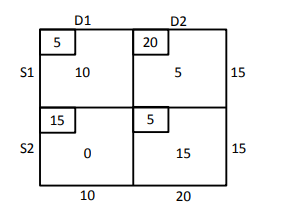
\includegraphics[width=0.75\columnwidth]{chapters/10/7/2/4/figs/fig.png}
 \end{center}
\caption{}
\label{fig:10/7/2/4Fig1}
\end{figure}
\fi

\item Find the position vector of the mid point of the vector joining the points $\vec{P}$(2, 3, 4)
and $\vec{Q}$(4, 1, –2).
\\
\solution
		\begin{enumerate}[label=\thesubsection.\arabic*,ref=\thesubsection.\theenumi]
\item Find the coordinates of the point which divides the join of $(-1,7) $ and $ (4,-3)$ in the ratio 2:3.
	\\
		\solution
	\input{chapters/10/7/2/1/section.tex}
\item Find the coordinates of the point $\vec{R}$ on the line segment joining the points $\vec{P}(-1,3)$ and $\vec{Q}(2,5)$ such that $PR=\frac{3}{5}PQ$.
\item Find the ratio in which the point $\vec{P}\brak{\frac{3}{4},\frac{5}{12}}$ divides the line segment joining the points $\vec{A}\brak{\frac{1}{2},\frac{3}{2}}$ and $ \vec{B}(2,-5)$.
\item Find the coordinates of the point which divides the line segment joining the points $(4,-3)$ and $(8,5)$ in the ratio $3:1$ internally.
\item Find the coordinates of the point $\vec{P}$ on $AD$ such that $AP : PD = 2 : 1$.
\item If the point $\vec{P} (2, 1)$ lies on the line segment joining points $\vec{A} (4, 2)$  and $ \vec{B} (8, 4)$,
then
\begin{enumerate}
	\item $AP =\frac{1}{3}{AB}$ 
\item ${AP}={PE}$
\item ${PB}=\frac{1}{3}{AB}$
\item${AP}=\frac{1}{2}{AB}$
 \end{enumerate}
\item Find the ratio in which the line segment joining the points $(-3,10)$  and  $(6,-8)$  is divided by $ (-1,6)$.
	\\
		\solution
	\input{chapters/10/7/2/4/section.tex}
\item Find the position vector of the mid point of the vector joining the points $\vec{P}$(2, 3, 4)
and $\vec{Q}$(4, 1, –2).
\\
\solution
		\input{chapters/12/10/2/16/section.tex}
\item Let $\vec{A}(4, 2), \vec{B}(6, 5)$  and $ \vec{C}(1, 4)$ be the vertices of $\triangle ABC$.
\begin{enumerate}
\item If $\vec{A}$ and  $\vec{B}$ are $(-2,-2)$ and  $(2,-4)$, respectively, find the coordinates of $\vec{P}$ such that $AP= \frac {3}{7}AB$  and $ \vec{P}$ lies on the line segment $AB$.
	\\
		\solution
	\input{chapters/10/7/2/8/section.tex}
\item Find the coordinates of the points which divide the line segment joining $A(-2,2)$  and  $\vec{B}(2,8)$ into four equal parts.
	\\
		\solution
	\input{chapters/10/7/2/9/section.tex}
\item In what ratio does the point $(-4,6)$ divide the line segment joining the points $\vec{A}(-6,0)$ and $\vec{B}(3,-8)$?
\item Given that $\vec{P}(3,2,-4), \vec{Q}(5,4,-6)$ and $\vec{R}(9,8,-10)$ are collinear. Find the ratio in which $\vec{Q}$ divides $PR$.
\item Points $\vec{A}(-6,10),\vec{B}(-4,6)$  and  $\vec{C}(3,-8)$ are collinear such that $AB=  \frac{2}{9}AC$.
\item The point which divides the line segment joining the points $\vec{P} (7, –6) $  and  $\vec{Q}(3, 4)$ in the 
ratio 1 : 2 internally lies in  which quadrant?
\item Find the coordinates of the points of trisection of the line segment joining $(4,-1)$  and  $(-2,3)$.
	\\
		\solution
	\input{chapters/10/7/2/2/section.tex}
\item Find the coordinates of the points which trisect the line segment joining the points $\vec{P}(4,2,-6)$ and $\vec{Q}(10,-16,6)$.
\item Find the coordinates of the points of trisection (i.e. points dividing to three equal parts) of the line segment joining the points $\vec{A}(2,-2)$ and $\vec{B}(-7,4)$.
\item Point $\vec{P}(5,-3)$ is one of the two points of trisection of line segment joining the points $\vec{A}(7,-2)$ and $\vec{B}(1,-5)$
\item Find the position vector of a point $\vec{R}$ which divides the line joining two points $\vec{P}$
and $\vec{Q}$ whose position vectors are $\hat{i}+2\hat{j}-\hat{k}$ and $-\hat{i}+\hat{j}+\hat{k}$ respectively, in the
ratio 2 : 1
\begin{enumerate}
    \item  internally
    \item  externally
\end{enumerate}
%\solution
%		\input{chapters/12/10/2/15/section.tex}
\item Find the coordinates of the point which divides the line segment joining the points which divides the line segment joining  the points $(-2,3,5)$ and $(1,-4,6)$ in the ratio 
\begin{enumerate}
\item $2:3$ internally,
\item $2:3$ externally
\end{enumerate}
\item Find the coordinates of the point which divides the line segment joining the points $(1,-2,3)$ and $(3,4,-5)$ in the ratio $2:3$
\begin{enumerate}
\item internally, and
\item externally
\end{enumerate}
\item Consider two points $\vec{P}$ and $\vec{Q}$ with position vectors $\overrightarrow{OP} = 3\overrightarrow{a}-2\overrightarrow{b}$ and $\overrightarrow{OQ}=\overrightarrow{a}+\overrightarrow{b}$. Find the position vector of a point $\vec{R}$ which divides the line joining $\vec{P}$ and $\vec{Q}$ in the ratio $2:1$, 
\begin{enumerate}
\item internally, and 
\item externally.
\end{enumerate}
\item The median from $\vec{A}$ meets $BC$ at $\vec{D}$. Find the coordinates of the point $\vec{D}$.
\item Find the coordinates of points $\vec{Q}$ and $\vec{R}$ on medians $BE$ and $CF$ respectively such that $BQ : QE = 2 : 1$  and  $CR : RF = 2 : 1$.
\item What do you observe?
\item If $\vec{A}, \vec{B}$ and $\vec{C}$  are the vertices of $\triangle ABC$, find the coordinates of the centroid of the triangle.
\end{enumerate}
\solution
	\input{chapters/10/7/4/7/section.tex}
\item If $\vec{P}(9a-2,-b)$ divides line segment joining $\vec{A}(3a+1,-3)$ and $\vec{B}(8a,5)$ in the ratio 3:1, find the values of $a$ and $b$.
\item Find the position vector of a point $\vec{R}$ which divides the line joining two points $\vec{P}$ and $\vec{Q}$ whose position vectors are $2\vec{a}+\vec{b}$ and $\vec{a}-3\vec{b}$ externally in the ratio $1:2$.
\item The position vector of the point which divides the join of points 2$\vec{a}$-3$\vec{b}$ $\text{and}$ $\vec{a}+\vec{b}$ in the ratio 3:1 is \rule{1cm}{0.1pt}.
\item If $\vec{a}$ and $\vec{b}$ are the postion vectors of $\vec{A}$ and $\vec{B}$, respectively, find the position vector of a point $\vec{C}$ in $BA$ produced such that $BC=1.5BA$.
\item Find the position vector of a point $\vec{R}$ which divides the line joining two points $\vec{P}$ and $\vec{Q}$ whose position vectors are $(2\vec{a}+\vec{b})$ and $(\vec{a}-3\vec{b})$
externally in the ratio 1 : 2. Also, show that $\vec{P}$ is the mid point of the line segment $RQ$.
\end{enumerate}

\item Let $\vec{A}(4, 2), \vec{B}(6, 5)$  and $ \vec{C}(1, 4)$ be the vertices of $\triangle ABC$.
\begin{enumerate}
\item If $\vec{A}$ and  $\vec{B}$ are $(-2,-2)$ and  $(2,-4)$, respectively, find the coordinates of $\vec{P}$ such that $AP= \frac {3}{7}AB$  and $ \vec{P}$ lies on the line segment $AB$.
	\\
		\solution
	\begin{enumerate}[label=\thesubsection.\arabic*,ref=\thesubsection.\theenumi]
\item Find the coordinates of the point which divides the join of $(-1,7) $ and $ (4,-3)$ in the ratio 2:3.
	\\
		\solution
	\input{chapters/10/7/2/1/section.tex}
\item Find the coordinates of the point $\vec{R}$ on the line segment joining the points $\vec{P}(-1,3)$ and $\vec{Q}(2,5)$ such that $PR=\frac{3}{5}PQ$.
\item Find the ratio in which the point $\vec{P}\brak{\frac{3}{4},\frac{5}{12}}$ divides the line segment joining the points $\vec{A}\brak{\frac{1}{2},\frac{3}{2}}$ and $ \vec{B}(2,-5)$.
\item Find the coordinates of the point which divides the line segment joining the points $(4,-3)$ and $(8,5)$ in the ratio $3:1$ internally.
\item Find the coordinates of the point $\vec{P}$ on $AD$ such that $AP : PD = 2 : 1$.
\item If the point $\vec{P} (2, 1)$ lies on the line segment joining points $\vec{A} (4, 2)$  and $ \vec{B} (8, 4)$,
then
\begin{enumerate}
	\item $AP =\frac{1}{3}{AB}$ 
\item ${AP}={PE}$
\item ${PB}=\frac{1}{3}{AB}$
\item${AP}=\frac{1}{2}{AB}$
 \end{enumerate}
\item Find the ratio in which the line segment joining the points $(-3,10)$  and  $(6,-8)$  is divided by $ (-1,6)$.
	\\
		\solution
	\input{chapters/10/7/2/4/section.tex}
\item Find the position vector of the mid point of the vector joining the points $\vec{P}$(2, 3, 4)
and $\vec{Q}$(4, 1, –2).
\\
\solution
		\input{chapters/12/10/2/16/section.tex}
\item Let $\vec{A}(4, 2), \vec{B}(6, 5)$  and $ \vec{C}(1, 4)$ be the vertices of $\triangle ABC$.
\begin{enumerate}
\item If $\vec{A}$ and  $\vec{B}$ are $(-2,-2)$ and  $(2,-4)$, respectively, find the coordinates of $\vec{P}$ such that $AP= \frac {3}{7}AB$  and $ \vec{P}$ lies on the line segment $AB$.
	\\
		\solution
	\input{chapters/10/7/2/8/section.tex}
\item Find the coordinates of the points which divide the line segment joining $A(-2,2)$  and  $\vec{B}(2,8)$ into four equal parts.
	\\
		\solution
	\input{chapters/10/7/2/9/section.tex}
\item In what ratio does the point $(-4,6)$ divide the line segment joining the points $\vec{A}(-6,0)$ and $\vec{B}(3,-8)$?
\item Given that $\vec{P}(3,2,-4), \vec{Q}(5,4,-6)$ and $\vec{R}(9,8,-10)$ are collinear. Find the ratio in which $\vec{Q}$ divides $PR$.
\item Points $\vec{A}(-6,10),\vec{B}(-4,6)$  and  $\vec{C}(3,-8)$ are collinear such that $AB=  \frac{2}{9}AC$.
\item The point which divides the line segment joining the points $\vec{P} (7, –6) $  and  $\vec{Q}(3, 4)$ in the 
ratio 1 : 2 internally lies in  which quadrant?
\item Find the coordinates of the points of trisection of the line segment joining $(4,-1)$  and  $(-2,3)$.
	\\
		\solution
	\input{chapters/10/7/2/2/section.tex}
\item Find the coordinates of the points which trisect the line segment joining the points $\vec{P}(4,2,-6)$ and $\vec{Q}(10,-16,6)$.
\item Find the coordinates of the points of trisection (i.e. points dividing to three equal parts) of the line segment joining the points $\vec{A}(2,-2)$ and $\vec{B}(-7,4)$.
\item Point $\vec{P}(5,-3)$ is one of the two points of trisection of line segment joining the points $\vec{A}(7,-2)$ and $\vec{B}(1,-5)$
\item Find the position vector of a point $\vec{R}$ which divides the line joining two points $\vec{P}$
and $\vec{Q}$ whose position vectors are $\hat{i}+2\hat{j}-\hat{k}$ and $-\hat{i}+\hat{j}+\hat{k}$ respectively, in the
ratio 2 : 1
\begin{enumerate}
    \item  internally
    \item  externally
\end{enumerate}
%\solution
%		\input{chapters/12/10/2/15/section.tex}
\item Find the coordinates of the point which divides the line segment joining the points which divides the line segment joining  the points $(-2,3,5)$ and $(1,-4,6)$ in the ratio 
\begin{enumerate}
\item $2:3$ internally,
\item $2:3$ externally
\end{enumerate}
\item Find the coordinates of the point which divides the line segment joining the points $(1,-2,3)$ and $(3,4,-5)$ in the ratio $2:3$
\begin{enumerate}
\item internally, and
\item externally
\end{enumerate}
\item Consider two points $\vec{P}$ and $\vec{Q}$ with position vectors $\overrightarrow{OP} = 3\overrightarrow{a}-2\overrightarrow{b}$ and $\overrightarrow{OQ}=\overrightarrow{a}+\overrightarrow{b}$. Find the position vector of a point $\vec{R}$ which divides the line joining $\vec{P}$ and $\vec{Q}$ in the ratio $2:1$, 
\begin{enumerate}
\item internally, and 
\item externally.
\end{enumerate}
\item The median from $\vec{A}$ meets $BC$ at $\vec{D}$. Find the coordinates of the point $\vec{D}$.
\item Find the coordinates of points $\vec{Q}$ and $\vec{R}$ on medians $BE$ and $CF$ respectively such that $BQ : QE = 2 : 1$  and  $CR : RF = 2 : 1$.
\item What do you observe?
\item If $\vec{A}, \vec{B}$ and $\vec{C}$  are the vertices of $\triangle ABC$, find the coordinates of the centroid of the triangle.
\end{enumerate}
\solution
	\input{chapters/10/7/4/7/section.tex}
\item If $\vec{P}(9a-2,-b)$ divides line segment joining $\vec{A}(3a+1,-3)$ and $\vec{B}(8a,5)$ in the ratio 3:1, find the values of $a$ and $b$.
\item Find the position vector of a point $\vec{R}$ which divides the line joining two points $\vec{P}$ and $\vec{Q}$ whose position vectors are $2\vec{a}+\vec{b}$ and $\vec{a}-3\vec{b}$ externally in the ratio $1:2$.
\item The position vector of the point which divides the join of points 2$\vec{a}$-3$\vec{b}$ $\text{and}$ $\vec{a}+\vec{b}$ in the ratio 3:1 is \rule{1cm}{0.1pt}.
\item If $\vec{a}$ and $\vec{b}$ are the postion vectors of $\vec{A}$ and $\vec{B}$, respectively, find the position vector of a point $\vec{C}$ in $BA$ produced such that $BC=1.5BA$.
\item Find the position vector of a point $\vec{R}$ which divides the line joining two points $\vec{P}$ and $\vec{Q}$ whose position vectors are $(2\vec{a}+\vec{b})$ and $(\vec{a}-3\vec{b})$
externally in the ratio 1 : 2. Also, show that $\vec{P}$ is the mid point of the line segment $RQ$.
\end{enumerate}

\item Find the coordinates of the points which divide the line segment joining $A(-2,2)$  and  $\vec{B}(2,8)$ into four equal parts.
	\\
		\solution
	\begin{enumerate}[label=\thesubsection.\arabic*,ref=\thesubsection.\theenumi]
\item Find the coordinates of the point which divides the join of $(-1,7) $ and $ (4,-3)$ in the ratio 2:3.
	\\
		\solution
	\input{chapters/10/7/2/1/section.tex}
\item Find the coordinates of the point $\vec{R}$ on the line segment joining the points $\vec{P}(-1,3)$ and $\vec{Q}(2,5)$ such that $PR=\frac{3}{5}PQ$.
\item Find the ratio in which the point $\vec{P}\brak{\frac{3}{4},\frac{5}{12}}$ divides the line segment joining the points $\vec{A}\brak{\frac{1}{2},\frac{3}{2}}$ and $ \vec{B}(2,-5)$.
\item Find the coordinates of the point which divides the line segment joining the points $(4,-3)$ and $(8,5)$ in the ratio $3:1$ internally.
\item Find the coordinates of the point $\vec{P}$ on $AD$ such that $AP : PD = 2 : 1$.
\item If the point $\vec{P} (2, 1)$ lies on the line segment joining points $\vec{A} (4, 2)$  and $ \vec{B} (8, 4)$,
then
\begin{enumerate}
	\item $AP =\frac{1}{3}{AB}$ 
\item ${AP}={PE}$
\item ${PB}=\frac{1}{3}{AB}$
\item${AP}=\frac{1}{2}{AB}$
 \end{enumerate}
\item Find the ratio in which the line segment joining the points $(-3,10)$  and  $(6,-8)$  is divided by $ (-1,6)$.
	\\
		\solution
	\input{chapters/10/7/2/4/section.tex}
\item Find the position vector of the mid point of the vector joining the points $\vec{P}$(2, 3, 4)
and $\vec{Q}$(4, 1, –2).
\\
\solution
		\input{chapters/12/10/2/16/section.tex}
\item Let $\vec{A}(4, 2), \vec{B}(6, 5)$  and $ \vec{C}(1, 4)$ be the vertices of $\triangle ABC$.
\begin{enumerate}
\item If $\vec{A}$ and  $\vec{B}$ are $(-2,-2)$ and  $(2,-4)$, respectively, find the coordinates of $\vec{P}$ such that $AP= \frac {3}{7}AB$  and $ \vec{P}$ lies on the line segment $AB$.
	\\
		\solution
	\input{chapters/10/7/2/8/section.tex}
\item Find the coordinates of the points which divide the line segment joining $A(-2,2)$  and  $\vec{B}(2,8)$ into four equal parts.
	\\
		\solution
	\input{chapters/10/7/2/9/section.tex}
\item In what ratio does the point $(-4,6)$ divide the line segment joining the points $\vec{A}(-6,0)$ and $\vec{B}(3,-8)$?
\item Given that $\vec{P}(3,2,-4), \vec{Q}(5,4,-6)$ and $\vec{R}(9,8,-10)$ are collinear. Find the ratio in which $\vec{Q}$ divides $PR$.
\item Points $\vec{A}(-6,10),\vec{B}(-4,6)$  and  $\vec{C}(3,-8)$ are collinear such that $AB=  \frac{2}{9}AC$.
\item The point which divides the line segment joining the points $\vec{P} (7, –6) $  and  $\vec{Q}(3, 4)$ in the 
ratio 1 : 2 internally lies in  which quadrant?
\item Find the coordinates of the points of trisection of the line segment joining $(4,-1)$  and  $(-2,3)$.
	\\
		\solution
	\input{chapters/10/7/2/2/section.tex}
\item Find the coordinates of the points which trisect the line segment joining the points $\vec{P}(4,2,-6)$ and $\vec{Q}(10,-16,6)$.
\item Find the coordinates of the points of trisection (i.e. points dividing to three equal parts) of the line segment joining the points $\vec{A}(2,-2)$ and $\vec{B}(-7,4)$.
\item Point $\vec{P}(5,-3)$ is one of the two points of trisection of line segment joining the points $\vec{A}(7,-2)$ and $\vec{B}(1,-5)$
\item Find the position vector of a point $\vec{R}$ which divides the line joining two points $\vec{P}$
and $\vec{Q}$ whose position vectors are $\hat{i}+2\hat{j}-\hat{k}$ and $-\hat{i}+\hat{j}+\hat{k}$ respectively, in the
ratio 2 : 1
\begin{enumerate}
    \item  internally
    \item  externally
\end{enumerate}
%\solution
%		\input{chapters/12/10/2/15/section.tex}
\item Find the coordinates of the point which divides the line segment joining the points which divides the line segment joining  the points $(-2,3,5)$ and $(1,-4,6)$ in the ratio 
\begin{enumerate}
\item $2:3$ internally,
\item $2:3$ externally
\end{enumerate}
\item Find the coordinates of the point which divides the line segment joining the points $(1,-2,3)$ and $(3,4,-5)$ in the ratio $2:3$
\begin{enumerate}
\item internally, and
\item externally
\end{enumerate}
\item Consider two points $\vec{P}$ and $\vec{Q}$ with position vectors $\overrightarrow{OP} = 3\overrightarrow{a}-2\overrightarrow{b}$ and $\overrightarrow{OQ}=\overrightarrow{a}+\overrightarrow{b}$. Find the position vector of a point $\vec{R}$ which divides the line joining $\vec{P}$ and $\vec{Q}$ in the ratio $2:1$, 
\begin{enumerate}
\item internally, and 
\item externally.
\end{enumerate}
\item The median from $\vec{A}$ meets $BC$ at $\vec{D}$. Find the coordinates of the point $\vec{D}$.
\item Find the coordinates of points $\vec{Q}$ and $\vec{R}$ on medians $BE$ and $CF$ respectively such that $BQ : QE = 2 : 1$  and  $CR : RF = 2 : 1$.
\item What do you observe?
\item If $\vec{A}, \vec{B}$ and $\vec{C}$  are the vertices of $\triangle ABC$, find the coordinates of the centroid of the triangle.
\end{enumerate}
\solution
	\input{chapters/10/7/4/7/section.tex}
\item If $\vec{P}(9a-2,-b)$ divides line segment joining $\vec{A}(3a+1,-3)$ and $\vec{B}(8a,5)$ in the ratio 3:1, find the values of $a$ and $b$.
\item Find the position vector of a point $\vec{R}$ which divides the line joining two points $\vec{P}$ and $\vec{Q}$ whose position vectors are $2\vec{a}+\vec{b}$ and $\vec{a}-3\vec{b}$ externally in the ratio $1:2$.
\item The position vector of the point which divides the join of points 2$\vec{a}$-3$\vec{b}$ $\text{and}$ $\vec{a}+\vec{b}$ in the ratio 3:1 is \rule{1cm}{0.1pt}.
\item If $\vec{a}$ and $\vec{b}$ are the postion vectors of $\vec{A}$ and $\vec{B}$, respectively, find the position vector of a point $\vec{C}$ in $BA$ produced such that $BC=1.5BA$.
\item Find the position vector of a point $\vec{R}$ which divides the line joining two points $\vec{P}$ and $\vec{Q}$ whose position vectors are $(2\vec{a}+\vec{b})$ and $(\vec{a}-3\vec{b})$
externally in the ratio 1 : 2. Also, show that $\vec{P}$ is the mid point of the line segment $RQ$.
\end{enumerate}

\item In what ratio does the point $(-4,6)$ divide the line segment joining the points $\vec{A}(-6,0)$ and $\vec{B}(3,-8)$?
\item Given that $\vec{P}(3,2,-4), \vec{Q}(5,4,-6)$ and $\vec{R}(9,8,-10)$ are collinear. Find the ratio in which $\vec{Q}$ divides $PR$.
\item Points $\vec{A}(-6,10),\vec{B}(-4,6)$  and  $\vec{C}(3,-8)$ are collinear such that $AB=  \frac{2}{9}AC$.
\item The point which divides the line segment joining the points $\vec{P} (7, –6) $  and  $\vec{Q}(3, 4)$ in the 
ratio 1 : 2 internally lies in  which quadrant?
\item Find the coordinates of the points of trisection of the line segment joining $(4,-1)$  and  $(-2,3)$.
	\\
		\solution
	Using section formula,
\begin{align}
\vec{R}=\frac{1}{1+\frac{1}{2}}\brak{\myvec{4\\-1}+\frac{1}{2}\myvec{-2\\3}}
=\myvec{2\\ \frac{1}{3}}\\
\vec{S}=\frac{1}{1+\frac{2}{1}}\brak{\myvec{4\\-1}+\frac{2}{1}\myvec{-2\\3}}
=\myvec{0\\ \frac{5}{3}}
\end{align}
which are the desired points of trisection.
\iffalse
See
		\figref{fig:chapters/10/7/2/2/Figure}
\begin{figure}[H]
\centering
\includegraphics[width=0.75\columnwidth]{chapters/10/7/2/2/figs/dj.pdf}
\caption{}
		\label{fig:chapters/10/7/2/2/Figure}
\end{figure}
\fi

\item Find the coordinates of the points which trisect the line segment joining the points $\vec{P}(4,2,-6)$ and $\vec{Q}(10,-16,6)$.
\item Find the coordinates of the points of trisection (i.e. points dividing to three equal parts) of the line segment joining the points $\vec{A}(2,-2)$ and $\vec{B}(-7,4)$.
\item Point $\vec{P}(5,-3)$ is one of the two points of trisection of line segment joining the points $\vec{A}(7,-2)$ and $\vec{B}(1,-5)$
\item Find the position vector of a point $\vec{R}$ which divides the line joining two points $\vec{P}$
and $\vec{Q}$ whose position vectors are $\hat{i}+2\hat{j}-\hat{k}$ and $-\hat{i}+\hat{j}+\hat{k}$ respectively, in the
ratio 2 : 1
\begin{enumerate}
    \item  internally
    \item  externally
\end{enumerate}
%\solution
%		\begin{enumerate}[label=\thesubsection.\arabic*,ref=\thesubsection.\theenumi]
\item Find the coordinates of the point which divides the join of $(-1,7) $ and $ (4,-3)$ in the ratio 2:3.
	\\
		\solution
	\input{chapters/10/7/2/1/section.tex}
\item Find the coordinates of the point $\vec{R}$ on the line segment joining the points $\vec{P}(-1,3)$ and $\vec{Q}(2,5)$ such that $PR=\frac{3}{5}PQ$.
\item Find the ratio in which the point $\vec{P}\brak{\frac{3}{4},\frac{5}{12}}$ divides the line segment joining the points $\vec{A}\brak{\frac{1}{2},\frac{3}{2}}$ and $ \vec{B}(2,-5)$.
\item Find the coordinates of the point which divides the line segment joining the points $(4,-3)$ and $(8,5)$ in the ratio $3:1$ internally.
\item Find the coordinates of the point $\vec{P}$ on $AD$ such that $AP : PD = 2 : 1$.
\item If the point $\vec{P} (2, 1)$ lies on the line segment joining points $\vec{A} (4, 2)$  and $ \vec{B} (8, 4)$,
then
\begin{enumerate}
	\item $AP =\frac{1}{3}{AB}$ 
\item ${AP}={PE}$
\item ${PB}=\frac{1}{3}{AB}$
\item${AP}=\frac{1}{2}{AB}$
 \end{enumerate}
\item Find the ratio in which the line segment joining the points $(-3,10)$  and  $(6,-8)$  is divided by $ (-1,6)$.
	\\
		\solution
	\input{chapters/10/7/2/4/section.tex}
\item Find the position vector of the mid point of the vector joining the points $\vec{P}$(2, 3, 4)
and $\vec{Q}$(4, 1, –2).
\\
\solution
		\input{chapters/12/10/2/16/section.tex}
\item Let $\vec{A}(4, 2), \vec{B}(6, 5)$  and $ \vec{C}(1, 4)$ be the vertices of $\triangle ABC$.
\begin{enumerate}
\item If $\vec{A}$ and  $\vec{B}$ are $(-2,-2)$ and  $(2,-4)$, respectively, find the coordinates of $\vec{P}$ such that $AP= \frac {3}{7}AB$  and $ \vec{P}$ lies on the line segment $AB$.
	\\
		\solution
	\input{chapters/10/7/2/8/section.tex}
\item Find the coordinates of the points which divide the line segment joining $A(-2,2)$  and  $\vec{B}(2,8)$ into four equal parts.
	\\
		\solution
	\input{chapters/10/7/2/9/section.tex}
\item In what ratio does the point $(-4,6)$ divide the line segment joining the points $\vec{A}(-6,0)$ and $\vec{B}(3,-8)$?
\item Given that $\vec{P}(3,2,-4), \vec{Q}(5,4,-6)$ and $\vec{R}(9,8,-10)$ are collinear. Find the ratio in which $\vec{Q}$ divides $PR$.
\item Points $\vec{A}(-6,10),\vec{B}(-4,6)$  and  $\vec{C}(3,-8)$ are collinear such that $AB=  \frac{2}{9}AC$.
\item The point which divides the line segment joining the points $\vec{P} (7, –6) $  and  $\vec{Q}(3, 4)$ in the 
ratio 1 : 2 internally lies in  which quadrant?
\item Find the coordinates of the points of trisection of the line segment joining $(4,-1)$  and  $(-2,3)$.
	\\
		\solution
	\input{chapters/10/7/2/2/section.tex}
\item Find the coordinates of the points which trisect the line segment joining the points $\vec{P}(4,2,-6)$ and $\vec{Q}(10,-16,6)$.
\item Find the coordinates of the points of trisection (i.e. points dividing to three equal parts) of the line segment joining the points $\vec{A}(2,-2)$ and $\vec{B}(-7,4)$.
\item Point $\vec{P}(5,-3)$ is one of the two points of trisection of line segment joining the points $\vec{A}(7,-2)$ and $\vec{B}(1,-5)$
\item Find the position vector of a point $\vec{R}$ which divides the line joining two points $\vec{P}$
and $\vec{Q}$ whose position vectors are $\hat{i}+2\hat{j}-\hat{k}$ and $-\hat{i}+\hat{j}+\hat{k}$ respectively, in the
ratio 2 : 1
\begin{enumerate}
    \item  internally
    \item  externally
\end{enumerate}
%\solution
%		\input{chapters/12/10/2/15/section.tex}
\item Find the coordinates of the point which divides the line segment joining the points which divides the line segment joining  the points $(-2,3,5)$ and $(1,-4,6)$ in the ratio 
\begin{enumerate}
\item $2:3$ internally,
\item $2:3$ externally
\end{enumerate}
\item Find the coordinates of the point which divides the line segment joining the points $(1,-2,3)$ and $(3,4,-5)$ in the ratio $2:3$
\begin{enumerate}
\item internally, and
\item externally
\end{enumerate}
\item Consider two points $\vec{P}$ and $\vec{Q}$ with position vectors $\overrightarrow{OP} = 3\overrightarrow{a}-2\overrightarrow{b}$ and $\overrightarrow{OQ}=\overrightarrow{a}+\overrightarrow{b}$. Find the position vector of a point $\vec{R}$ which divides the line joining $\vec{P}$ and $\vec{Q}$ in the ratio $2:1$, 
\begin{enumerate}
\item internally, and 
\item externally.
\end{enumerate}
\item The median from $\vec{A}$ meets $BC$ at $\vec{D}$. Find the coordinates of the point $\vec{D}$.
\item Find the coordinates of points $\vec{Q}$ and $\vec{R}$ on medians $BE$ and $CF$ respectively such that $BQ : QE = 2 : 1$  and  $CR : RF = 2 : 1$.
\item What do you observe?
\item If $\vec{A}, \vec{B}$ and $\vec{C}$  are the vertices of $\triangle ABC$, find the coordinates of the centroid of the triangle.
\end{enumerate}
\solution
	\input{chapters/10/7/4/7/section.tex}
\item If $\vec{P}(9a-2,-b)$ divides line segment joining $\vec{A}(3a+1,-3)$ and $\vec{B}(8a,5)$ in the ratio 3:1, find the values of $a$ and $b$.
\item Find the position vector of a point $\vec{R}$ which divides the line joining two points $\vec{P}$ and $\vec{Q}$ whose position vectors are $2\vec{a}+\vec{b}$ and $\vec{a}-3\vec{b}$ externally in the ratio $1:2$.
\item The position vector of the point which divides the join of points 2$\vec{a}$-3$\vec{b}$ $\text{and}$ $\vec{a}+\vec{b}$ in the ratio 3:1 is \rule{1cm}{0.1pt}.
\item If $\vec{a}$ and $\vec{b}$ are the postion vectors of $\vec{A}$ and $\vec{B}$, respectively, find the position vector of a point $\vec{C}$ in $BA$ produced such that $BC=1.5BA$.
\item Find the position vector of a point $\vec{R}$ which divides the line joining two points $\vec{P}$ and $\vec{Q}$ whose position vectors are $(2\vec{a}+\vec{b})$ and $(\vec{a}-3\vec{b})$
externally in the ratio 1 : 2. Also, show that $\vec{P}$ is the mid point of the line segment $RQ$.
\end{enumerate}

\item Find the coordinates of the point which divides the line segment joining the points which divides the line segment joining  the points $(-2,3,5)$ and $(1,-4,6)$ in the ratio 
\begin{enumerate}
\item $2:3$ internally,
\item $2:3$ externally
\end{enumerate}
\item Find the coordinates of the point which divides the line segment joining the points $(1,-2,3)$ and $(3,4,-5)$ in the ratio $2:3$
\begin{enumerate}
\item internally, and
\item externally
\end{enumerate}
\item Consider two points $\vec{P}$ and $\vec{Q}$ with position vectors $\overrightarrow{OP} = 3\overrightarrow{a}-2\overrightarrow{b}$ and $\overrightarrow{OQ}=\overrightarrow{a}+\overrightarrow{b}$. Find the position vector of a point $\vec{R}$ which divides the line joining $\vec{P}$ and $\vec{Q}$ in the ratio $2:1$, 
\begin{enumerate}
\item internally, and 
\item externally.
\end{enumerate}
\item The median from $\vec{A}$ meets $BC$ at $\vec{D}$. Find the coordinates of the point $\vec{D}$.
\item Find the coordinates of points $\vec{Q}$ and $\vec{R}$ on medians $BE$ and $CF$ respectively such that $BQ : QE = 2 : 1$  and  $CR : RF = 2 : 1$.
\item What do you observe?
\item If $\vec{A}, \vec{B}$ and $\vec{C}$  are the vertices of $\triangle ABC$, find the coordinates of the centroid of the triangle.
\end{enumerate}
\solution
	\begin{enumerate}[label=\thesubsection.\arabic*,ref=\thesubsection.\theenumi]
\item Find the coordinates of the point which divides the join of $(-1,7) $ and $ (4,-3)$ in the ratio 2:3.
	\\
		\solution
	\input{chapters/10/7/2/1/section.tex}
\item Find the coordinates of the point $\vec{R}$ on the line segment joining the points $\vec{P}(-1,3)$ and $\vec{Q}(2,5)$ such that $PR=\frac{3}{5}PQ$.
\item Find the ratio in which the point $\vec{P}\brak{\frac{3}{4},\frac{5}{12}}$ divides the line segment joining the points $\vec{A}\brak{\frac{1}{2},\frac{3}{2}}$ and $ \vec{B}(2,-5)$.
\item Find the coordinates of the point which divides the line segment joining the points $(4,-3)$ and $(8,5)$ in the ratio $3:1$ internally.
\item Find the coordinates of the point $\vec{P}$ on $AD$ such that $AP : PD = 2 : 1$.
\item If the point $\vec{P} (2, 1)$ lies on the line segment joining points $\vec{A} (4, 2)$  and $ \vec{B} (8, 4)$,
then
\begin{enumerate}
	\item $AP =\frac{1}{3}{AB}$ 
\item ${AP}={PE}$
\item ${PB}=\frac{1}{3}{AB}$
\item${AP}=\frac{1}{2}{AB}$
 \end{enumerate}
\item Find the ratio in which the line segment joining the points $(-3,10)$  and  $(6,-8)$  is divided by $ (-1,6)$.
	\\
		\solution
	\input{chapters/10/7/2/4/section.tex}
\item Find the position vector of the mid point of the vector joining the points $\vec{P}$(2, 3, 4)
and $\vec{Q}$(4, 1, –2).
\\
\solution
		\input{chapters/12/10/2/16/section.tex}
\item Let $\vec{A}(4, 2), \vec{B}(6, 5)$  and $ \vec{C}(1, 4)$ be the vertices of $\triangle ABC$.
\begin{enumerate}
\item If $\vec{A}$ and  $\vec{B}$ are $(-2,-2)$ and  $(2,-4)$, respectively, find the coordinates of $\vec{P}$ such that $AP= \frac {3}{7}AB$  and $ \vec{P}$ lies on the line segment $AB$.
	\\
		\solution
	\input{chapters/10/7/2/8/section.tex}
\item Find the coordinates of the points which divide the line segment joining $A(-2,2)$  and  $\vec{B}(2,8)$ into four equal parts.
	\\
		\solution
	\input{chapters/10/7/2/9/section.tex}
\item In what ratio does the point $(-4,6)$ divide the line segment joining the points $\vec{A}(-6,0)$ and $\vec{B}(3,-8)$?
\item Given that $\vec{P}(3,2,-4), \vec{Q}(5,4,-6)$ and $\vec{R}(9,8,-10)$ are collinear. Find the ratio in which $\vec{Q}$ divides $PR$.
\item Points $\vec{A}(-6,10),\vec{B}(-4,6)$  and  $\vec{C}(3,-8)$ are collinear such that $AB=  \frac{2}{9}AC$.
\item The point which divides the line segment joining the points $\vec{P} (7, –6) $  and  $\vec{Q}(3, 4)$ in the 
ratio 1 : 2 internally lies in  which quadrant?
\item Find the coordinates of the points of trisection of the line segment joining $(4,-1)$  and  $(-2,3)$.
	\\
		\solution
	\input{chapters/10/7/2/2/section.tex}
\item Find the coordinates of the points which trisect the line segment joining the points $\vec{P}(4,2,-6)$ and $\vec{Q}(10,-16,6)$.
\item Find the coordinates of the points of trisection (i.e. points dividing to three equal parts) of the line segment joining the points $\vec{A}(2,-2)$ and $\vec{B}(-7,4)$.
\item Point $\vec{P}(5,-3)$ is one of the two points of trisection of line segment joining the points $\vec{A}(7,-2)$ and $\vec{B}(1,-5)$
\item Find the position vector of a point $\vec{R}$ which divides the line joining two points $\vec{P}$
and $\vec{Q}$ whose position vectors are $\hat{i}+2\hat{j}-\hat{k}$ and $-\hat{i}+\hat{j}+\hat{k}$ respectively, in the
ratio 2 : 1
\begin{enumerate}
    \item  internally
    \item  externally
\end{enumerate}
%\solution
%		\input{chapters/12/10/2/15/section.tex}
\item Find the coordinates of the point which divides the line segment joining the points which divides the line segment joining  the points $(-2,3,5)$ and $(1,-4,6)$ in the ratio 
\begin{enumerate}
\item $2:3$ internally,
\item $2:3$ externally
\end{enumerate}
\item Find the coordinates of the point which divides the line segment joining the points $(1,-2,3)$ and $(3,4,-5)$ in the ratio $2:3$
\begin{enumerate}
\item internally, and
\item externally
\end{enumerate}
\item Consider two points $\vec{P}$ and $\vec{Q}$ with position vectors $\overrightarrow{OP} = 3\overrightarrow{a}-2\overrightarrow{b}$ and $\overrightarrow{OQ}=\overrightarrow{a}+\overrightarrow{b}$. Find the position vector of a point $\vec{R}$ which divides the line joining $\vec{P}$ and $\vec{Q}$ in the ratio $2:1$, 
\begin{enumerate}
\item internally, and 
\item externally.
\end{enumerate}
\item The median from $\vec{A}$ meets $BC$ at $\vec{D}$. Find the coordinates of the point $\vec{D}$.
\item Find the coordinates of points $\vec{Q}$ and $\vec{R}$ on medians $BE$ and $CF$ respectively such that $BQ : QE = 2 : 1$  and  $CR : RF = 2 : 1$.
\item What do you observe?
\item If $\vec{A}, \vec{B}$ and $\vec{C}$  are the vertices of $\triangle ABC$, find the coordinates of the centroid of the triangle.
\end{enumerate}
\solution
	\input{chapters/10/7/4/7/section.tex}
\item If $\vec{P}(9a-2,-b)$ divides line segment joining $\vec{A}(3a+1,-3)$ and $\vec{B}(8a,5)$ in the ratio 3:1, find the values of $a$ and $b$.
\item Find the position vector of a point $\vec{R}$ which divides the line joining two points $\vec{P}$ and $\vec{Q}$ whose position vectors are $2\vec{a}+\vec{b}$ and $\vec{a}-3\vec{b}$ externally in the ratio $1:2$.
\item The position vector of the point which divides the join of points 2$\vec{a}$-3$\vec{b}$ $\text{and}$ $\vec{a}+\vec{b}$ in the ratio 3:1 is \rule{1cm}{0.1pt}.
\item If $\vec{a}$ and $\vec{b}$ are the postion vectors of $\vec{A}$ and $\vec{B}$, respectively, find the position vector of a point $\vec{C}$ in $BA$ produced such that $BC=1.5BA$.
\item Find the position vector of a point $\vec{R}$ which divides the line joining two points $\vec{P}$ and $\vec{Q}$ whose position vectors are $(2\vec{a}+\vec{b})$ and $(\vec{a}-3\vec{b})$
externally in the ratio 1 : 2. Also, show that $\vec{P}$ is the mid point of the line segment $RQ$.
\end{enumerate}

\item If $\vec{P}(9a-2,-b)$ divides line segment joining $\vec{A}(3a+1,-3)$ and $\vec{B}(8a,5)$ in the ratio 3:1, find the values of $a$ and $b$.
\item Find the position vector of a point $\vec{R}$ which divides the line joining two points $\vec{P}$ and $\vec{Q}$ whose position vectors are $2\vec{a}+\vec{b}$ and $\vec{a}-3\vec{b}$ externally in the ratio $1:2$.
\item The position vector of the point which divides the join of points 2$\vec{a}$-3$\vec{b}$ $\text{and}$ $\vec{a}+\vec{b}$ in the ratio 3:1 is \rule{1cm}{0.1pt}.
\item If $\vec{a}$ and $\vec{b}$ are the postion vectors of $\vec{A}$ and $\vec{B}$, respectively, find the position vector of a point $\vec{C}$ in $BA$ produced such that $BC=1.5BA$.
\item Find the position vector of a point $\vec{R}$ which divides the line joining two points $\vec{P}$ and $\vec{Q}$ whose position vectors are $(2\vec{a}+\vec{b})$ and $(\vec{a}-3\vec{b})$
externally in the ratio 1 : 2. Also, show that $\vec{P}$ is the mid point of the line segment $RQ$.
\end{enumerate}

\item Find the coordinates of the point which divides the line segment joining the points which divides the line segment joining  the points $(-2,3,5)$ and $(1,-4,6)$ in the ratio 
\begin{enumerate}
\item $2:3$ internally,
\item $2:3$ externally
\end{enumerate}
\item Find the coordinates of the point which divides the line segment joining the points $(1,-2,3)$ and $(3,4,-5)$ in the ratio $2:3$
\begin{enumerate}
\item internally, and
\item externally
\end{enumerate}
\item Consider two points $\vec{P}$ and $\vec{Q}$ with position vectors $\overrightarrow{OP} = 3\overrightarrow{a}-2\overrightarrow{b}$ and $\overrightarrow{OQ}=\overrightarrow{a}+\overrightarrow{b}$. Find the position vector of a point $\vec{R}$ which divides the line joining $\vec{P}$ and $\vec{Q}$ in the ratio $2:1$, 
\begin{enumerate}
\item internally, and 
\item externally.
\end{enumerate}
\item The median from $\vec{A}$ meets $BC$ at $\vec{D}$. Find the coordinates of the point $\vec{D}$.
\item Find the coordinates of points $\vec{Q}$ and $\vec{R}$ on medians $BE$ and $CF$ respectively such that $BQ : QE = 2 : 1$  and  $CR : RF = 2 : 1$.
\item What do you observe?
\item If $\vec{A}, \vec{B}$ and $\vec{C}$  are the vertices of $\triangle ABC$, find the coordinates of the centroid of the triangle.
\end{enumerate}
\solution
	\begin{enumerate}[label=\thesubsection.\arabic*,ref=\thesubsection.\theenumi]
\item Find the coordinates of the point which divides the join of $(-1,7) $ and $ (4,-3)$ in the ratio 2:3.
	\\
		\solution
	\begin{enumerate}[label=\thesubsection.\arabic*,ref=\thesubsection.\theenumi]
\item Find the coordinates of the point which divides the join of $(-1,7) $ and $ (4,-3)$ in the ratio 2:3.
	\\
		\solution
	\input{chapters/10/7/2/1/section.tex}
\item Find the coordinates of the point $\vec{R}$ on the line segment joining the points $\vec{P}(-1,3)$ and $\vec{Q}(2,5)$ such that $PR=\frac{3}{5}PQ$.
\item Find the ratio in which the point $\vec{P}\brak{\frac{3}{4},\frac{5}{12}}$ divides the line segment joining the points $\vec{A}\brak{\frac{1}{2},\frac{3}{2}}$ and $ \vec{B}(2,-5)$.
\item Find the coordinates of the point which divides the line segment joining the points $(4,-3)$ and $(8,5)$ in the ratio $3:1$ internally.
\item Find the coordinates of the point $\vec{P}$ on $AD$ such that $AP : PD = 2 : 1$.
\item If the point $\vec{P} (2, 1)$ lies on the line segment joining points $\vec{A} (4, 2)$  and $ \vec{B} (8, 4)$,
then
\begin{enumerate}
	\item $AP =\frac{1}{3}{AB}$ 
\item ${AP}={PE}$
\item ${PB}=\frac{1}{3}{AB}$
\item${AP}=\frac{1}{2}{AB}$
 \end{enumerate}
\item Find the ratio in which the line segment joining the points $(-3,10)$  and  $(6,-8)$  is divided by $ (-1,6)$.
	\\
		\solution
	\input{chapters/10/7/2/4/section.tex}
\item Find the position vector of the mid point of the vector joining the points $\vec{P}$(2, 3, 4)
and $\vec{Q}$(4, 1, –2).
\\
\solution
		\input{chapters/12/10/2/16/section.tex}
\item Let $\vec{A}(4, 2), \vec{B}(6, 5)$  and $ \vec{C}(1, 4)$ be the vertices of $\triangle ABC$.
\begin{enumerate}
\item If $\vec{A}$ and  $\vec{B}$ are $(-2,-2)$ and  $(2,-4)$, respectively, find the coordinates of $\vec{P}$ such that $AP= \frac {3}{7}AB$  and $ \vec{P}$ lies on the line segment $AB$.
	\\
		\solution
	\input{chapters/10/7/2/8/section.tex}
\item Find the coordinates of the points which divide the line segment joining $A(-2,2)$  and  $\vec{B}(2,8)$ into four equal parts.
	\\
		\solution
	\input{chapters/10/7/2/9/section.tex}
\item In what ratio does the point $(-4,6)$ divide the line segment joining the points $\vec{A}(-6,0)$ and $\vec{B}(3,-8)$?
\item Given that $\vec{P}(3,2,-4), \vec{Q}(5,4,-6)$ and $\vec{R}(9,8,-10)$ are collinear. Find the ratio in which $\vec{Q}$ divides $PR$.
\item Points $\vec{A}(-6,10),\vec{B}(-4,6)$  and  $\vec{C}(3,-8)$ are collinear such that $AB=  \frac{2}{9}AC$.
\item The point which divides the line segment joining the points $\vec{P} (7, –6) $  and  $\vec{Q}(3, 4)$ in the 
ratio 1 : 2 internally lies in  which quadrant?
\item Find the coordinates of the points of trisection of the line segment joining $(4,-1)$  and  $(-2,3)$.
	\\
		\solution
	\input{chapters/10/7/2/2/section.tex}
\item Find the coordinates of the points which trisect the line segment joining the points $\vec{P}(4,2,-6)$ and $\vec{Q}(10,-16,6)$.
\item Find the coordinates of the points of trisection (i.e. points dividing to three equal parts) of the line segment joining the points $\vec{A}(2,-2)$ and $\vec{B}(-7,4)$.
\item Point $\vec{P}(5,-3)$ is one of the two points of trisection of line segment joining the points $\vec{A}(7,-2)$ and $\vec{B}(1,-5)$
\item Find the position vector of a point $\vec{R}$ which divides the line joining two points $\vec{P}$
and $\vec{Q}$ whose position vectors are $\hat{i}+2\hat{j}-\hat{k}$ and $-\hat{i}+\hat{j}+\hat{k}$ respectively, in the
ratio 2 : 1
\begin{enumerate}
    \item  internally
    \item  externally
\end{enumerate}
%\solution
%		\input{chapters/12/10/2/15/section.tex}
\item Find the coordinates of the point which divides the line segment joining the points which divides the line segment joining  the points $(-2,3,5)$ and $(1,-4,6)$ in the ratio 
\begin{enumerate}
\item $2:3$ internally,
\item $2:3$ externally
\end{enumerate}
\item Find the coordinates of the point which divides the line segment joining the points $(1,-2,3)$ and $(3,4,-5)$ in the ratio $2:3$
\begin{enumerate}
\item internally, and
\item externally
\end{enumerate}
\item Consider two points $\vec{P}$ and $\vec{Q}$ with position vectors $\overrightarrow{OP} = 3\overrightarrow{a}-2\overrightarrow{b}$ and $\overrightarrow{OQ}=\overrightarrow{a}+\overrightarrow{b}$. Find the position vector of a point $\vec{R}$ which divides the line joining $\vec{P}$ and $\vec{Q}$ in the ratio $2:1$, 
\begin{enumerate}
\item internally, and 
\item externally.
\end{enumerate}
\item The median from $\vec{A}$ meets $BC$ at $\vec{D}$. Find the coordinates of the point $\vec{D}$.
\item Find the coordinates of points $\vec{Q}$ and $\vec{R}$ on medians $BE$ and $CF$ respectively such that $BQ : QE = 2 : 1$  and  $CR : RF = 2 : 1$.
\item What do you observe?
\item If $\vec{A}, \vec{B}$ and $\vec{C}$  are the vertices of $\triangle ABC$, find the coordinates of the centroid of the triangle.
\end{enumerate}
\solution
	\input{chapters/10/7/4/7/section.tex}
\item If $\vec{P}(9a-2,-b)$ divides line segment joining $\vec{A}(3a+1,-3)$ and $\vec{B}(8a,5)$ in the ratio 3:1, find the values of $a$ and $b$.
\item Find the position vector of a point $\vec{R}$ which divides the line joining two points $\vec{P}$ and $\vec{Q}$ whose position vectors are $2\vec{a}+\vec{b}$ and $\vec{a}-3\vec{b}$ externally in the ratio $1:2$.
\item The position vector of the point which divides the join of points 2$\vec{a}$-3$\vec{b}$ $\text{and}$ $\vec{a}+\vec{b}$ in the ratio 3:1 is \rule{1cm}{0.1pt}.
\item If $\vec{a}$ and $\vec{b}$ are the postion vectors of $\vec{A}$ and $\vec{B}$, respectively, find the position vector of a point $\vec{C}$ in $BA$ produced such that $BC=1.5BA$.
\item Find the position vector of a point $\vec{R}$ which divides the line joining two points $\vec{P}$ and $\vec{Q}$ whose position vectors are $(2\vec{a}+\vec{b})$ and $(\vec{a}-3\vec{b})$
externally in the ratio 1 : 2. Also, show that $\vec{P}$ is the mid point of the line segment $RQ$.
\end{enumerate}

\item Find the coordinates of the point $\vec{R}$ on the line segment joining the points $\vec{P}(-1,3)$ and $\vec{Q}(2,5)$ such that $PR=\frac{3}{5}PQ$.
\item Find the ratio in which the point $\vec{P}\brak{\frac{3}{4},\frac{5}{12}}$ divides the line segment joining the points $\vec{A}\brak{\frac{1}{2},\frac{3}{2}}$ and $ \vec{B}(2,-5)$.
\item Find the coordinates of the point which divides the line segment joining the points $(4,-3)$ and $(8,5)$ in the ratio $3:1$ internally.
\item Find the coordinates of the point $\vec{P}$ on $AD$ such that $AP : PD = 2 : 1$.
\item If the point $\vec{P} (2, 1)$ lies on the line segment joining points $\vec{A} (4, 2)$  and $ \vec{B} (8, 4)$,
then
\begin{enumerate}
	\item $AP =\frac{1}{3}{AB}$ 
\item ${AP}={PE}$
\item ${PB}=\frac{1}{3}{AB}$
\item${AP}=\frac{1}{2}{AB}$
 \end{enumerate}
\item Find the ratio in which the line segment joining the points $(-3,10)$  and  $(6,-8)$  is divided by $ (-1,6)$.
	\\
		\solution
	\iffalse
Using section formula,
\begin{align}
         \myvec{-1\\6} &=\frac{{\myvec{-3\\10}+k\myvec{6\\-8}}}{1+k}\\
	 \implies 7k\myvec{1 \\ -2} &= 2\myvec{1 \\ -2}
	 \\
	 \text{or, } k &= \frac{2}{7}.
\end{align}
\fi
In 
			\eqref{eq:section_formula-k}, substituting
			\begin{align}
				\vec{B} &= \myvec{-3\\10}, \vec{C} = \myvec{6\\-8}, \vec{D} = \myvec{-1\\6},
				\\
				k &= \frac{\myvec{-2 & 4}\myvec{-7 \\ 14}}{\norm{\myvec{-7 \\ 14}}^2} = \frac{2}{7}
			\end{align}
\iffalse
See \figref{fig:10/7/2/4Fig1}.
\begin{figure}[H]
 \begin{center}
  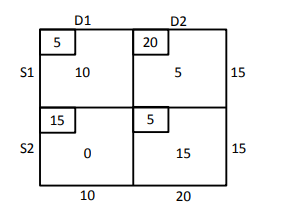
\includegraphics[width=0.75\columnwidth]{chapters/10/7/2/4/figs/fig.png}
 \end{center}
\caption{}
\label{fig:10/7/2/4Fig1}
\end{figure}
\fi

\item Find the position vector of the mid point of the vector joining the points $\vec{P}$(2, 3, 4)
and $\vec{Q}$(4, 1, –2).
\\
\solution
		\begin{enumerate}[label=\thesubsection.\arabic*,ref=\thesubsection.\theenumi]
\item Find the coordinates of the point which divides the join of $(-1,7) $ and $ (4,-3)$ in the ratio 2:3.
	\\
		\solution
	\input{chapters/10/7/2/1/section.tex}
\item Find the coordinates of the point $\vec{R}$ on the line segment joining the points $\vec{P}(-1,3)$ and $\vec{Q}(2,5)$ such that $PR=\frac{3}{5}PQ$.
\item Find the ratio in which the point $\vec{P}\brak{\frac{3}{4},\frac{5}{12}}$ divides the line segment joining the points $\vec{A}\brak{\frac{1}{2},\frac{3}{2}}$ and $ \vec{B}(2,-5)$.
\item Find the coordinates of the point which divides the line segment joining the points $(4,-3)$ and $(8,5)$ in the ratio $3:1$ internally.
\item Find the coordinates of the point $\vec{P}$ on $AD$ such that $AP : PD = 2 : 1$.
\item If the point $\vec{P} (2, 1)$ lies on the line segment joining points $\vec{A} (4, 2)$  and $ \vec{B} (8, 4)$,
then
\begin{enumerate}
	\item $AP =\frac{1}{3}{AB}$ 
\item ${AP}={PE}$
\item ${PB}=\frac{1}{3}{AB}$
\item${AP}=\frac{1}{2}{AB}$
 \end{enumerate}
\item Find the ratio in which the line segment joining the points $(-3,10)$  and  $(6,-8)$  is divided by $ (-1,6)$.
	\\
		\solution
	\input{chapters/10/7/2/4/section.tex}
\item Find the position vector of the mid point of the vector joining the points $\vec{P}$(2, 3, 4)
and $\vec{Q}$(4, 1, –2).
\\
\solution
		\input{chapters/12/10/2/16/section.tex}
\item Let $\vec{A}(4, 2), \vec{B}(6, 5)$  and $ \vec{C}(1, 4)$ be the vertices of $\triangle ABC$.
\begin{enumerate}
\item If $\vec{A}$ and  $\vec{B}$ are $(-2,-2)$ and  $(2,-4)$, respectively, find the coordinates of $\vec{P}$ such that $AP= \frac {3}{7}AB$  and $ \vec{P}$ lies on the line segment $AB$.
	\\
		\solution
	\input{chapters/10/7/2/8/section.tex}
\item Find the coordinates of the points which divide the line segment joining $A(-2,2)$  and  $\vec{B}(2,8)$ into four equal parts.
	\\
		\solution
	\input{chapters/10/7/2/9/section.tex}
\item In what ratio does the point $(-4,6)$ divide the line segment joining the points $\vec{A}(-6,0)$ and $\vec{B}(3,-8)$?
\item Given that $\vec{P}(3,2,-4), \vec{Q}(5,4,-6)$ and $\vec{R}(9,8,-10)$ are collinear. Find the ratio in which $\vec{Q}$ divides $PR$.
\item Points $\vec{A}(-6,10),\vec{B}(-4,6)$  and  $\vec{C}(3,-8)$ are collinear such that $AB=  \frac{2}{9}AC$.
\item The point which divides the line segment joining the points $\vec{P} (7, –6) $  and  $\vec{Q}(3, 4)$ in the 
ratio 1 : 2 internally lies in  which quadrant?
\item Find the coordinates of the points of trisection of the line segment joining $(4,-1)$  and  $(-2,3)$.
	\\
		\solution
	\input{chapters/10/7/2/2/section.tex}
\item Find the coordinates of the points which trisect the line segment joining the points $\vec{P}(4,2,-6)$ and $\vec{Q}(10,-16,6)$.
\item Find the coordinates of the points of trisection (i.e. points dividing to three equal parts) of the line segment joining the points $\vec{A}(2,-2)$ and $\vec{B}(-7,4)$.
\item Point $\vec{P}(5,-3)$ is one of the two points of trisection of line segment joining the points $\vec{A}(7,-2)$ and $\vec{B}(1,-5)$
\item Find the position vector of a point $\vec{R}$ which divides the line joining two points $\vec{P}$
and $\vec{Q}$ whose position vectors are $\hat{i}+2\hat{j}-\hat{k}$ and $-\hat{i}+\hat{j}+\hat{k}$ respectively, in the
ratio 2 : 1
\begin{enumerate}
    \item  internally
    \item  externally
\end{enumerate}
%\solution
%		\input{chapters/12/10/2/15/section.tex}
\item Find the coordinates of the point which divides the line segment joining the points which divides the line segment joining  the points $(-2,3,5)$ and $(1,-4,6)$ in the ratio 
\begin{enumerate}
\item $2:3$ internally,
\item $2:3$ externally
\end{enumerate}
\item Find the coordinates of the point which divides the line segment joining the points $(1,-2,3)$ and $(3,4,-5)$ in the ratio $2:3$
\begin{enumerate}
\item internally, and
\item externally
\end{enumerate}
\item Consider two points $\vec{P}$ and $\vec{Q}$ with position vectors $\overrightarrow{OP} = 3\overrightarrow{a}-2\overrightarrow{b}$ and $\overrightarrow{OQ}=\overrightarrow{a}+\overrightarrow{b}$. Find the position vector of a point $\vec{R}$ which divides the line joining $\vec{P}$ and $\vec{Q}$ in the ratio $2:1$, 
\begin{enumerate}
\item internally, and 
\item externally.
\end{enumerate}
\item The median from $\vec{A}$ meets $BC$ at $\vec{D}$. Find the coordinates of the point $\vec{D}$.
\item Find the coordinates of points $\vec{Q}$ and $\vec{R}$ on medians $BE$ and $CF$ respectively such that $BQ : QE = 2 : 1$  and  $CR : RF = 2 : 1$.
\item What do you observe?
\item If $\vec{A}, \vec{B}$ and $\vec{C}$  are the vertices of $\triangle ABC$, find the coordinates of the centroid of the triangle.
\end{enumerate}
\solution
	\input{chapters/10/7/4/7/section.tex}
\item If $\vec{P}(9a-2,-b)$ divides line segment joining $\vec{A}(3a+1,-3)$ and $\vec{B}(8a,5)$ in the ratio 3:1, find the values of $a$ and $b$.
\item Find the position vector of a point $\vec{R}$ which divides the line joining two points $\vec{P}$ and $\vec{Q}$ whose position vectors are $2\vec{a}+\vec{b}$ and $\vec{a}-3\vec{b}$ externally in the ratio $1:2$.
\item The position vector of the point which divides the join of points 2$\vec{a}$-3$\vec{b}$ $\text{and}$ $\vec{a}+\vec{b}$ in the ratio 3:1 is \rule{1cm}{0.1pt}.
\item If $\vec{a}$ and $\vec{b}$ are the postion vectors of $\vec{A}$ and $\vec{B}$, respectively, find the position vector of a point $\vec{C}$ in $BA$ produced such that $BC=1.5BA$.
\item Find the position vector of a point $\vec{R}$ which divides the line joining two points $\vec{P}$ and $\vec{Q}$ whose position vectors are $(2\vec{a}+\vec{b})$ and $(\vec{a}-3\vec{b})$
externally in the ratio 1 : 2. Also, show that $\vec{P}$ is the mid point of the line segment $RQ$.
\end{enumerate}

\item Let $\vec{A}(4, 2), \vec{B}(6, 5)$  and $ \vec{C}(1, 4)$ be the vertices of $\triangle ABC$.
\begin{enumerate}
\item If $\vec{A}$ and  $\vec{B}$ are $(-2,-2)$ and  $(2,-4)$, respectively, find the coordinates of $\vec{P}$ such that $AP= \frac {3}{7}AB$  and $ \vec{P}$ lies on the line segment $AB$.
	\\
		\solution
	\begin{enumerate}[label=\thesubsection.\arabic*,ref=\thesubsection.\theenumi]
\item Find the coordinates of the point which divides the join of $(-1,7) $ and $ (4,-3)$ in the ratio 2:3.
	\\
		\solution
	\input{chapters/10/7/2/1/section.tex}
\item Find the coordinates of the point $\vec{R}$ on the line segment joining the points $\vec{P}(-1,3)$ and $\vec{Q}(2,5)$ such that $PR=\frac{3}{5}PQ$.
\item Find the ratio in which the point $\vec{P}\brak{\frac{3}{4},\frac{5}{12}}$ divides the line segment joining the points $\vec{A}\brak{\frac{1}{2},\frac{3}{2}}$ and $ \vec{B}(2,-5)$.
\item Find the coordinates of the point which divides the line segment joining the points $(4,-3)$ and $(8,5)$ in the ratio $3:1$ internally.
\item Find the coordinates of the point $\vec{P}$ on $AD$ such that $AP : PD = 2 : 1$.
\item If the point $\vec{P} (2, 1)$ lies on the line segment joining points $\vec{A} (4, 2)$  and $ \vec{B} (8, 4)$,
then
\begin{enumerate}
	\item $AP =\frac{1}{3}{AB}$ 
\item ${AP}={PE}$
\item ${PB}=\frac{1}{3}{AB}$
\item${AP}=\frac{1}{2}{AB}$
 \end{enumerate}
\item Find the ratio in which the line segment joining the points $(-3,10)$  and  $(6,-8)$  is divided by $ (-1,6)$.
	\\
		\solution
	\input{chapters/10/7/2/4/section.tex}
\item Find the position vector of the mid point of the vector joining the points $\vec{P}$(2, 3, 4)
and $\vec{Q}$(4, 1, –2).
\\
\solution
		\input{chapters/12/10/2/16/section.tex}
\item Let $\vec{A}(4, 2), \vec{B}(6, 5)$  and $ \vec{C}(1, 4)$ be the vertices of $\triangle ABC$.
\begin{enumerate}
\item If $\vec{A}$ and  $\vec{B}$ are $(-2,-2)$ and  $(2,-4)$, respectively, find the coordinates of $\vec{P}$ such that $AP= \frac {3}{7}AB$  and $ \vec{P}$ lies on the line segment $AB$.
	\\
		\solution
	\input{chapters/10/7/2/8/section.tex}
\item Find the coordinates of the points which divide the line segment joining $A(-2,2)$  and  $\vec{B}(2,8)$ into four equal parts.
	\\
		\solution
	\input{chapters/10/7/2/9/section.tex}
\item In what ratio does the point $(-4,6)$ divide the line segment joining the points $\vec{A}(-6,0)$ and $\vec{B}(3,-8)$?
\item Given that $\vec{P}(3,2,-4), \vec{Q}(5,4,-6)$ and $\vec{R}(9,8,-10)$ are collinear. Find the ratio in which $\vec{Q}$ divides $PR$.
\item Points $\vec{A}(-6,10),\vec{B}(-4,6)$  and  $\vec{C}(3,-8)$ are collinear such that $AB=  \frac{2}{9}AC$.
\item The point which divides the line segment joining the points $\vec{P} (7, –6) $  and  $\vec{Q}(3, 4)$ in the 
ratio 1 : 2 internally lies in  which quadrant?
\item Find the coordinates of the points of trisection of the line segment joining $(4,-1)$  and  $(-2,3)$.
	\\
		\solution
	\input{chapters/10/7/2/2/section.tex}
\item Find the coordinates of the points which trisect the line segment joining the points $\vec{P}(4,2,-6)$ and $\vec{Q}(10,-16,6)$.
\item Find the coordinates of the points of trisection (i.e. points dividing to three equal parts) of the line segment joining the points $\vec{A}(2,-2)$ and $\vec{B}(-7,4)$.
\item Point $\vec{P}(5,-3)$ is one of the two points of trisection of line segment joining the points $\vec{A}(7,-2)$ and $\vec{B}(1,-5)$
\item Find the position vector of a point $\vec{R}$ which divides the line joining two points $\vec{P}$
and $\vec{Q}$ whose position vectors are $\hat{i}+2\hat{j}-\hat{k}$ and $-\hat{i}+\hat{j}+\hat{k}$ respectively, in the
ratio 2 : 1
\begin{enumerate}
    \item  internally
    \item  externally
\end{enumerate}
%\solution
%		\input{chapters/12/10/2/15/section.tex}
\item Find the coordinates of the point which divides the line segment joining the points which divides the line segment joining  the points $(-2,3,5)$ and $(1,-4,6)$ in the ratio 
\begin{enumerate}
\item $2:3$ internally,
\item $2:3$ externally
\end{enumerate}
\item Find the coordinates of the point which divides the line segment joining the points $(1,-2,3)$ and $(3,4,-5)$ in the ratio $2:3$
\begin{enumerate}
\item internally, and
\item externally
\end{enumerate}
\item Consider two points $\vec{P}$ and $\vec{Q}$ with position vectors $\overrightarrow{OP} = 3\overrightarrow{a}-2\overrightarrow{b}$ and $\overrightarrow{OQ}=\overrightarrow{a}+\overrightarrow{b}$. Find the position vector of a point $\vec{R}$ which divides the line joining $\vec{P}$ and $\vec{Q}$ in the ratio $2:1$, 
\begin{enumerate}
\item internally, and 
\item externally.
\end{enumerate}
\item The median from $\vec{A}$ meets $BC$ at $\vec{D}$. Find the coordinates of the point $\vec{D}$.
\item Find the coordinates of points $\vec{Q}$ and $\vec{R}$ on medians $BE$ and $CF$ respectively such that $BQ : QE = 2 : 1$  and  $CR : RF = 2 : 1$.
\item What do you observe?
\item If $\vec{A}, \vec{B}$ and $\vec{C}$  are the vertices of $\triangle ABC$, find the coordinates of the centroid of the triangle.
\end{enumerate}
\solution
	\input{chapters/10/7/4/7/section.tex}
\item If $\vec{P}(9a-2,-b)$ divides line segment joining $\vec{A}(3a+1,-3)$ and $\vec{B}(8a,5)$ in the ratio 3:1, find the values of $a$ and $b$.
\item Find the position vector of a point $\vec{R}$ which divides the line joining two points $\vec{P}$ and $\vec{Q}$ whose position vectors are $2\vec{a}+\vec{b}$ and $\vec{a}-3\vec{b}$ externally in the ratio $1:2$.
\item The position vector of the point which divides the join of points 2$\vec{a}$-3$\vec{b}$ $\text{and}$ $\vec{a}+\vec{b}$ in the ratio 3:1 is \rule{1cm}{0.1pt}.
\item If $\vec{a}$ and $\vec{b}$ are the postion vectors of $\vec{A}$ and $\vec{B}$, respectively, find the position vector of a point $\vec{C}$ in $BA$ produced such that $BC=1.5BA$.
\item Find the position vector of a point $\vec{R}$ which divides the line joining two points $\vec{P}$ and $\vec{Q}$ whose position vectors are $(2\vec{a}+\vec{b})$ and $(\vec{a}-3\vec{b})$
externally in the ratio 1 : 2. Also, show that $\vec{P}$ is the mid point of the line segment $RQ$.
\end{enumerate}

\item Find the coordinates of the points which divide the line segment joining $A(-2,2)$  and  $\vec{B}(2,8)$ into four equal parts.
	\\
		\solution
	\begin{enumerate}[label=\thesubsection.\arabic*,ref=\thesubsection.\theenumi]
\item Find the coordinates of the point which divides the join of $(-1,7) $ and $ (4,-3)$ in the ratio 2:3.
	\\
		\solution
	\input{chapters/10/7/2/1/section.tex}
\item Find the coordinates of the point $\vec{R}$ on the line segment joining the points $\vec{P}(-1,3)$ and $\vec{Q}(2,5)$ such that $PR=\frac{3}{5}PQ$.
\item Find the ratio in which the point $\vec{P}\brak{\frac{3}{4},\frac{5}{12}}$ divides the line segment joining the points $\vec{A}\brak{\frac{1}{2},\frac{3}{2}}$ and $ \vec{B}(2,-5)$.
\item Find the coordinates of the point which divides the line segment joining the points $(4,-3)$ and $(8,5)$ in the ratio $3:1$ internally.
\item Find the coordinates of the point $\vec{P}$ on $AD$ such that $AP : PD = 2 : 1$.
\item If the point $\vec{P} (2, 1)$ lies on the line segment joining points $\vec{A} (4, 2)$  and $ \vec{B} (8, 4)$,
then
\begin{enumerate}
	\item $AP =\frac{1}{3}{AB}$ 
\item ${AP}={PE}$
\item ${PB}=\frac{1}{3}{AB}$
\item${AP}=\frac{1}{2}{AB}$
 \end{enumerate}
\item Find the ratio in which the line segment joining the points $(-3,10)$  and  $(6,-8)$  is divided by $ (-1,6)$.
	\\
		\solution
	\input{chapters/10/7/2/4/section.tex}
\item Find the position vector of the mid point of the vector joining the points $\vec{P}$(2, 3, 4)
and $\vec{Q}$(4, 1, –2).
\\
\solution
		\input{chapters/12/10/2/16/section.tex}
\item Let $\vec{A}(4, 2), \vec{B}(6, 5)$  and $ \vec{C}(1, 4)$ be the vertices of $\triangle ABC$.
\begin{enumerate}
\item If $\vec{A}$ and  $\vec{B}$ are $(-2,-2)$ and  $(2,-4)$, respectively, find the coordinates of $\vec{P}$ such that $AP= \frac {3}{7}AB$  and $ \vec{P}$ lies on the line segment $AB$.
	\\
		\solution
	\input{chapters/10/7/2/8/section.tex}
\item Find the coordinates of the points which divide the line segment joining $A(-2,2)$  and  $\vec{B}(2,8)$ into four equal parts.
	\\
		\solution
	\input{chapters/10/7/2/9/section.tex}
\item In what ratio does the point $(-4,6)$ divide the line segment joining the points $\vec{A}(-6,0)$ and $\vec{B}(3,-8)$?
\item Given that $\vec{P}(3,2,-4), \vec{Q}(5,4,-6)$ and $\vec{R}(9,8,-10)$ are collinear. Find the ratio in which $\vec{Q}$ divides $PR$.
\item Points $\vec{A}(-6,10),\vec{B}(-4,6)$  and  $\vec{C}(3,-8)$ are collinear such that $AB=  \frac{2}{9}AC$.
\item The point which divides the line segment joining the points $\vec{P} (7, –6) $  and  $\vec{Q}(3, 4)$ in the 
ratio 1 : 2 internally lies in  which quadrant?
\item Find the coordinates of the points of trisection of the line segment joining $(4,-1)$  and  $(-2,3)$.
	\\
		\solution
	\input{chapters/10/7/2/2/section.tex}
\item Find the coordinates of the points which trisect the line segment joining the points $\vec{P}(4,2,-6)$ and $\vec{Q}(10,-16,6)$.
\item Find the coordinates of the points of trisection (i.e. points dividing to three equal parts) of the line segment joining the points $\vec{A}(2,-2)$ and $\vec{B}(-7,4)$.
\item Point $\vec{P}(5,-3)$ is one of the two points of trisection of line segment joining the points $\vec{A}(7,-2)$ and $\vec{B}(1,-5)$
\item Find the position vector of a point $\vec{R}$ which divides the line joining two points $\vec{P}$
and $\vec{Q}$ whose position vectors are $\hat{i}+2\hat{j}-\hat{k}$ and $-\hat{i}+\hat{j}+\hat{k}$ respectively, in the
ratio 2 : 1
\begin{enumerate}
    \item  internally
    \item  externally
\end{enumerate}
%\solution
%		\input{chapters/12/10/2/15/section.tex}
\item Find the coordinates of the point which divides the line segment joining the points which divides the line segment joining  the points $(-2,3,5)$ and $(1,-4,6)$ in the ratio 
\begin{enumerate}
\item $2:3$ internally,
\item $2:3$ externally
\end{enumerate}
\item Find the coordinates of the point which divides the line segment joining the points $(1,-2,3)$ and $(3,4,-5)$ in the ratio $2:3$
\begin{enumerate}
\item internally, and
\item externally
\end{enumerate}
\item Consider two points $\vec{P}$ and $\vec{Q}$ with position vectors $\overrightarrow{OP} = 3\overrightarrow{a}-2\overrightarrow{b}$ and $\overrightarrow{OQ}=\overrightarrow{a}+\overrightarrow{b}$. Find the position vector of a point $\vec{R}$ which divides the line joining $\vec{P}$ and $\vec{Q}$ in the ratio $2:1$, 
\begin{enumerate}
\item internally, and 
\item externally.
\end{enumerate}
\item The median from $\vec{A}$ meets $BC$ at $\vec{D}$. Find the coordinates of the point $\vec{D}$.
\item Find the coordinates of points $\vec{Q}$ and $\vec{R}$ on medians $BE$ and $CF$ respectively such that $BQ : QE = 2 : 1$  and  $CR : RF = 2 : 1$.
\item What do you observe?
\item If $\vec{A}, \vec{B}$ and $\vec{C}$  are the vertices of $\triangle ABC$, find the coordinates of the centroid of the triangle.
\end{enumerate}
\solution
	\input{chapters/10/7/4/7/section.tex}
\item If $\vec{P}(9a-2,-b)$ divides line segment joining $\vec{A}(3a+1,-3)$ and $\vec{B}(8a,5)$ in the ratio 3:1, find the values of $a$ and $b$.
\item Find the position vector of a point $\vec{R}$ which divides the line joining two points $\vec{P}$ and $\vec{Q}$ whose position vectors are $2\vec{a}+\vec{b}$ and $\vec{a}-3\vec{b}$ externally in the ratio $1:2$.
\item The position vector of the point which divides the join of points 2$\vec{a}$-3$\vec{b}$ $\text{and}$ $\vec{a}+\vec{b}$ in the ratio 3:1 is \rule{1cm}{0.1pt}.
\item If $\vec{a}$ and $\vec{b}$ are the postion vectors of $\vec{A}$ and $\vec{B}$, respectively, find the position vector of a point $\vec{C}$ in $BA$ produced such that $BC=1.5BA$.
\item Find the position vector of a point $\vec{R}$ which divides the line joining two points $\vec{P}$ and $\vec{Q}$ whose position vectors are $(2\vec{a}+\vec{b})$ and $(\vec{a}-3\vec{b})$
externally in the ratio 1 : 2. Also, show that $\vec{P}$ is the mid point of the line segment $RQ$.
\end{enumerate}

\item In what ratio does the point $(-4,6)$ divide the line segment joining the points $\vec{A}(-6,0)$ and $\vec{B}(3,-8)$?
\item Given that $\vec{P}(3,2,-4), \vec{Q}(5,4,-6)$ and $\vec{R}(9,8,-10)$ are collinear. Find the ratio in which $\vec{Q}$ divides $PR$.
\item Points $\vec{A}(-6,10),\vec{B}(-4,6)$  and  $\vec{C}(3,-8)$ are collinear such that $AB=  \frac{2}{9}AC$.
\item The point which divides the line segment joining the points $\vec{P} (7, –6) $  and  $\vec{Q}(3, 4)$ in the 
ratio 1 : 2 internally lies in  which quadrant?
\item Find the coordinates of the points of trisection of the line segment joining $(4,-1)$  and  $(-2,3)$.
	\\
		\solution
	Using section formula,
\begin{align}
\vec{R}=\frac{1}{1+\frac{1}{2}}\brak{\myvec{4\\-1}+\frac{1}{2}\myvec{-2\\3}}
=\myvec{2\\ \frac{1}{3}}\\
\vec{S}=\frac{1}{1+\frac{2}{1}}\brak{\myvec{4\\-1}+\frac{2}{1}\myvec{-2\\3}}
=\myvec{0\\ \frac{5}{3}}
\end{align}
which are the desired points of trisection.
\iffalse
See
		\figref{fig:chapters/10/7/2/2/Figure}
\begin{figure}[H]
\centering
\includegraphics[width=0.75\columnwidth]{chapters/10/7/2/2/figs/dj.pdf}
\caption{}
		\label{fig:chapters/10/7/2/2/Figure}
\end{figure}
\fi

\item Find the coordinates of the points which trisect the line segment joining the points $\vec{P}(4,2,-6)$ and $\vec{Q}(10,-16,6)$.
\item Find the coordinates of the points of trisection (i.e. points dividing to three equal parts) of the line segment joining the points $\vec{A}(2,-2)$ and $\vec{B}(-7,4)$.
\item Point $\vec{P}(5,-3)$ is one of the two points of trisection of line segment joining the points $\vec{A}(7,-2)$ and $\vec{B}(1,-5)$
\item Find the position vector of a point $\vec{R}$ which divides the line joining two points $\vec{P}$
and $\vec{Q}$ whose position vectors are $\hat{i}+2\hat{j}-\hat{k}$ and $-\hat{i}+\hat{j}+\hat{k}$ respectively, in the
ratio 2 : 1
\begin{enumerate}
    \item  internally
    \item  externally
\end{enumerate}
%\solution
%		\begin{enumerate}[label=\thesubsection.\arabic*,ref=\thesubsection.\theenumi]
\item Find the coordinates of the point which divides the join of $(-1,7) $ and $ (4,-3)$ in the ratio 2:3.
	\\
		\solution
	\input{chapters/10/7/2/1/section.tex}
\item Find the coordinates of the point $\vec{R}$ on the line segment joining the points $\vec{P}(-1,3)$ and $\vec{Q}(2,5)$ such that $PR=\frac{3}{5}PQ$.
\item Find the ratio in which the point $\vec{P}\brak{\frac{3}{4},\frac{5}{12}}$ divides the line segment joining the points $\vec{A}\brak{\frac{1}{2},\frac{3}{2}}$ and $ \vec{B}(2,-5)$.
\item Find the coordinates of the point which divides the line segment joining the points $(4,-3)$ and $(8,5)$ in the ratio $3:1$ internally.
\item Find the coordinates of the point $\vec{P}$ on $AD$ such that $AP : PD = 2 : 1$.
\item If the point $\vec{P} (2, 1)$ lies on the line segment joining points $\vec{A} (4, 2)$  and $ \vec{B} (8, 4)$,
then
\begin{enumerate}
	\item $AP =\frac{1}{3}{AB}$ 
\item ${AP}={PE}$
\item ${PB}=\frac{1}{3}{AB}$
\item${AP}=\frac{1}{2}{AB}$
 \end{enumerate}
\item Find the ratio in which the line segment joining the points $(-3,10)$  and  $(6,-8)$  is divided by $ (-1,6)$.
	\\
		\solution
	\input{chapters/10/7/2/4/section.tex}
\item Find the position vector of the mid point of the vector joining the points $\vec{P}$(2, 3, 4)
and $\vec{Q}$(4, 1, –2).
\\
\solution
		\input{chapters/12/10/2/16/section.tex}
\item Let $\vec{A}(4, 2), \vec{B}(6, 5)$  and $ \vec{C}(1, 4)$ be the vertices of $\triangle ABC$.
\begin{enumerate}
\item If $\vec{A}$ and  $\vec{B}$ are $(-2,-2)$ and  $(2,-4)$, respectively, find the coordinates of $\vec{P}$ such that $AP= \frac {3}{7}AB$  and $ \vec{P}$ lies on the line segment $AB$.
	\\
		\solution
	\input{chapters/10/7/2/8/section.tex}
\item Find the coordinates of the points which divide the line segment joining $A(-2,2)$  and  $\vec{B}(2,8)$ into four equal parts.
	\\
		\solution
	\input{chapters/10/7/2/9/section.tex}
\item In what ratio does the point $(-4,6)$ divide the line segment joining the points $\vec{A}(-6,0)$ and $\vec{B}(3,-8)$?
\item Given that $\vec{P}(3,2,-4), \vec{Q}(5,4,-6)$ and $\vec{R}(9,8,-10)$ are collinear. Find the ratio in which $\vec{Q}$ divides $PR$.
\item Points $\vec{A}(-6,10),\vec{B}(-4,6)$  and  $\vec{C}(3,-8)$ are collinear such that $AB=  \frac{2}{9}AC$.
\item The point which divides the line segment joining the points $\vec{P} (7, –6) $  and  $\vec{Q}(3, 4)$ in the 
ratio 1 : 2 internally lies in  which quadrant?
\item Find the coordinates of the points of trisection of the line segment joining $(4,-1)$  and  $(-2,3)$.
	\\
		\solution
	\input{chapters/10/7/2/2/section.tex}
\item Find the coordinates of the points which trisect the line segment joining the points $\vec{P}(4,2,-6)$ and $\vec{Q}(10,-16,6)$.
\item Find the coordinates of the points of trisection (i.e. points dividing to three equal parts) of the line segment joining the points $\vec{A}(2,-2)$ and $\vec{B}(-7,4)$.
\item Point $\vec{P}(5,-3)$ is one of the two points of trisection of line segment joining the points $\vec{A}(7,-2)$ and $\vec{B}(1,-5)$
\item Find the position vector of a point $\vec{R}$ which divides the line joining two points $\vec{P}$
and $\vec{Q}$ whose position vectors are $\hat{i}+2\hat{j}-\hat{k}$ and $-\hat{i}+\hat{j}+\hat{k}$ respectively, in the
ratio 2 : 1
\begin{enumerate}
    \item  internally
    \item  externally
\end{enumerate}
%\solution
%		\input{chapters/12/10/2/15/section.tex}
\item Find the coordinates of the point which divides the line segment joining the points which divides the line segment joining  the points $(-2,3,5)$ and $(1,-4,6)$ in the ratio 
\begin{enumerate}
\item $2:3$ internally,
\item $2:3$ externally
\end{enumerate}
\item Find the coordinates of the point which divides the line segment joining the points $(1,-2,3)$ and $(3,4,-5)$ in the ratio $2:3$
\begin{enumerate}
\item internally, and
\item externally
\end{enumerate}
\item Consider two points $\vec{P}$ and $\vec{Q}$ with position vectors $\overrightarrow{OP} = 3\overrightarrow{a}-2\overrightarrow{b}$ and $\overrightarrow{OQ}=\overrightarrow{a}+\overrightarrow{b}$. Find the position vector of a point $\vec{R}$ which divides the line joining $\vec{P}$ and $\vec{Q}$ in the ratio $2:1$, 
\begin{enumerate}
\item internally, and 
\item externally.
\end{enumerate}
\item The median from $\vec{A}$ meets $BC$ at $\vec{D}$. Find the coordinates of the point $\vec{D}$.
\item Find the coordinates of points $\vec{Q}$ and $\vec{R}$ on medians $BE$ and $CF$ respectively such that $BQ : QE = 2 : 1$  and  $CR : RF = 2 : 1$.
\item What do you observe?
\item If $\vec{A}, \vec{B}$ and $\vec{C}$  are the vertices of $\triangle ABC$, find the coordinates of the centroid of the triangle.
\end{enumerate}
\solution
	\input{chapters/10/7/4/7/section.tex}
\item If $\vec{P}(9a-2,-b)$ divides line segment joining $\vec{A}(3a+1,-3)$ and $\vec{B}(8a,5)$ in the ratio 3:1, find the values of $a$ and $b$.
\item Find the position vector of a point $\vec{R}$ which divides the line joining two points $\vec{P}$ and $\vec{Q}$ whose position vectors are $2\vec{a}+\vec{b}$ and $\vec{a}-3\vec{b}$ externally in the ratio $1:2$.
\item The position vector of the point which divides the join of points 2$\vec{a}$-3$\vec{b}$ $\text{and}$ $\vec{a}+\vec{b}$ in the ratio 3:1 is \rule{1cm}{0.1pt}.
\item If $\vec{a}$ and $\vec{b}$ are the postion vectors of $\vec{A}$ and $\vec{B}$, respectively, find the position vector of a point $\vec{C}$ in $BA$ produced such that $BC=1.5BA$.
\item Find the position vector of a point $\vec{R}$ which divides the line joining two points $\vec{P}$ and $\vec{Q}$ whose position vectors are $(2\vec{a}+\vec{b})$ and $(\vec{a}-3\vec{b})$
externally in the ratio 1 : 2. Also, show that $\vec{P}$ is the mid point of the line segment $RQ$.
\end{enumerate}

\item Find the coordinates of the point which divides the line segment joining the points which divides the line segment joining  the points $(-2,3,5)$ and $(1,-4,6)$ in the ratio 
\begin{enumerate}
\item $2:3$ internally,
\item $2:3$ externally
\end{enumerate}
\item Find the coordinates of the point which divides the line segment joining the points $(1,-2,3)$ and $(3,4,-5)$ in the ratio $2:3$
\begin{enumerate}
\item internally, and
\item externally
\end{enumerate}
\item Consider two points $\vec{P}$ and $\vec{Q}$ with position vectors $\overrightarrow{OP} = 3\overrightarrow{a}-2\overrightarrow{b}$ and $\overrightarrow{OQ}=\overrightarrow{a}+\overrightarrow{b}$. Find the position vector of a point $\vec{R}$ which divides the line joining $\vec{P}$ and $\vec{Q}$ in the ratio $2:1$, 
\begin{enumerate}
\item internally, and 
\item externally.
\end{enumerate}
\item The median from $\vec{A}$ meets $BC$ at $\vec{D}$. Find the coordinates of the point $\vec{D}$.
\item Find the coordinates of points $\vec{Q}$ and $\vec{R}$ on medians $BE$ and $CF$ respectively such that $BQ : QE = 2 : 1$  and  $CR : RF = 2 : 1$.
\item What do you observe?
\item If $\vec{A}, \vec{B}$ and $\vec{C}$  are the vertices of $\triangle ABC$, find the coordinates of the centroid of the triangle.
\end{enumerate}
\solution
	\begin{enumerate}[label=\thesubsection.\arabic*,ref=\thesubsection.\theenumi]
\item Find the coordinates of the point which divides the join of $(-1,7) $ and $ (4,-3)$ in the ratio 2:3.
	\\
		\solution
	\input{chapters/10/7/2/1/section.tex}
\item Find the coordinates of the point $\vec{R}$ on the line segment joining the points $\vec{P}(-1,3)$ and $\vec{Q}(2,5)$ such that $PR=\frac{3}{5}PQ$.
\item Find the ratio in which the point $\vec{P}\brak{\frac{3}{4},\frac{5}{12}}$ divides the line segment joining the points $\vec{A}\brak{\frac{1}{2},\frac{3}{2}}$ and $ \vec{B}(2,-5)$.
\item Find the coordinates of the point which divides the line segment joining the points $(4,-3)$ and $(8,5)$ in the ratio $3:1$ internally.
\item Find the coordinates of the point $\vec{P}$ on $AD$ such that $AP : PD = 2 : 1$.
\item If the point $\vec{P} (2, 1)$ lies on the line segment joining points $\vec{A} (4, 2)$  and $ \vec{B} (8, 4)$,
then
\begin{enumerate}
	\item $AP =\frac{1}{3}{AB}$ 
\item ${AP}={PE}$
\item ${PB}=\frac{1}{3}{AB}$
\item${AP}=\frac{1}{2}{AB}$
 \end{enumerate}
\item Find the ratio in which the line segment joining the points $(-3,10)$  and  $(6,-8)$  is divided by $ (-1,6)$.
	\\
		\solution
	\input{chapters/10/7/2/4/section.tex}
\item Find the position vector of the mid point of the vector joining the points $\vec{P}$(2, 3, 4)
and $\vec{Q}$(4, 1, –2).
\\
\solution
		\input{chapters/12/10/2/16/section.tex}
\item Let $\vec{A}(4, 2), \vec{B}(6, 5)$  and $ \vec{C}(1, 4)$ be the vertices of $\triangle ABC$.
\begin{enumerate}
\item If $\vec{A}$ and  $\vec{B}$ are $(-2,-2)$ and  $(2,-4)$, respectively, find the coordinates of $\vec{P}$ such that $AP= \frac {3}{7}AB$  and $ \vec{P}$ lies on the line segment $AB$.
	\\
		\solution
	\input{chapters/10/7/2/8/section.tex}
\item Find the coordinates of the points which divide the line segment joining $A(-2,2)$  and  $\vec{B}(2,8)$ into four equal parts.
	\\
		\solution
	\input{chapters/10/7/2/9/section.tex}
\item In what ratio does the point $(-4,6)$ divide the line segment joining the points $\vec{A}(-6,0)$ and $\vec{B}(3,-8)$?
\item Given that $\vec{P}(3,2,-4), \vec{Q}(5,4,-6)$ and $\vec{R}(9,8,-10)$ are collinear. Find the ratio in which $\vec{Q}$ divides $PR$.
\item Points $\vec{A}(-6,10),\vec{B}(-4,6)$  and  $\vec{C}(3,-8)$ are collinear such that $AB=  \frac{2}{9}AC$.
\item The point which divides the line segment joining the points $\vec{P} (7, –6) $  and  $\vec{Q}(3, 4)$ in the 
ratio 1 : 2 internally lies in  which quadrant?
\item Find the coordinates of the points of trisection of the line segment joining $(4,-1)$  and  $(-2,3)$.
	\\
		\solution
	\input{chapters/10/7/2/2/section.tex}
\item Find the coordinates of the points which trisect the line segment joining the points $\vec{P}(4,2,-6)$ and $\vec{Q}(10,-16,6)$.
\item Find the coordinates of the points of trisection (i.e. points dividing to three equal parts) of the line segment joining the points $\vec{A}(2,-2)$ and $\vec{B}(-7,4)$.
\item Point $\vec{P}(5,-3)$ is one of the two points of trisection of line segment joining the points $\vec{A}(7,-2)$ and $\vec{B}(1,-5)$
\item Find the position vector of a point $\vec{R}$ which divides the line joining two points $\vec{P}$
and $\vec{Q}$ whose position vectors are $\hat{i}+2\hat{j}-\hat{k}$ and $-\hat{i}+\hat{j}+\hat{k}$ respectively, in the
ratio 2 : 1
\begin{enumerate}
    \item  internally
    \item  externally
\end{enumerate}
%\solution
%		\input{chapters/12/10/2/15/section.tex}
\item Find the coordinates of the point which divides the line segment joining the points which divides the line segment joining  the points $(-2,3,5)$ and $(1,-4,6)$ in the ratio 
\begin{enumerate}
\item $2:3$ internally,
\item $2:3$ externally
\end{enumerate}
\item Find the coordinates of the point which divides the line segment joining the points $(1,-2,3)$ and $(3,4,-5)$ in the ratio $2:3$
\begin{enumerate}
\item internally, and
\item externally
\end{enumerate}
\item Consider two points $\vec{P}$ and $\vec{Q}$ with position vectors $\overrightarrow{OP} = 3\overrightarrow{a}-2\overrightarrow{b}$ and $\overrightarrow{OQ}=\overrightarrow{a}+\overrightarrow{b}$. Find the position vector of a point $\vec{R}$ which divides the line joining $\vec{P}$ and $\vec{Q}$ in the ratio $2:1$, 
\begin{enumerate}
\item internally, and 
\item externally.
\end{enumerate}
\item The median from $\vec{A}$ meets $BC$ at $\vec{D}$. Find the coordinates of the point $\vec{D}$.
\item Find the coordinates of points $\vec{Q}$ and $\vec{R}$ on medians $BE$ and $CF$ respectively such that $BQ : QE = 2 : 1$  and  $CR : RF = 2 : 1$.
\item What do you observe?
\item If $\vec{A}, \vec{B}$ and $\vec{C}$  are the vertices of $\triangle ABC$, find the coordinates of the centroid of the triangle.
\end{enumerate}
\solution
	\input{chapters/10/7/4/7/section.tex}
\item If $\vec{P}(9a-2,-b)$ divides line segment joining $\vec{A}(3a+1,-3)$ and $\vec{B}(8a,5)$ in the ratio 3:1, find the values of $a$ and $b$.
\item Find the position vector of a point $\vec{R}$ which divides the line joining two points $\vec{P}$ and $\vec{Q}$ whose position vectors are $2\vec{a}+\vec{b}$ and $\vec{a}-3\vec{b}$ externally in the ratio $1:2$.
\item The position vector of the point which divides the join of points 2$\vec{a}$-3$\vec{b}$ $\text{and}$ $\vec{a}+\vec{b}$ in the ratio 3:1 is \rule{1cm}{0.1pt}.
\item If $\vec{a}$ and $\vec{b}$ are the postion vectors of $\vec{A}$ and $\vec{B}$, respectively, find the position vector of a point $\vec{C}$ in $BA$ produced such that $BC=1.5BA$.
\item Find the position vector of a point $\vec{R}$ which divides the line joining two points $\vec{P}$ and $\vec{Q}$ whose position vectors are $(2\vec{a}+\vec{b})$ and $(\vec{a}-3\vec{b})$
externally in the ratio 1 : 2. Also, show that $\vec{P}$ is the mid point of the line segment $RQ$.
\end{enumerate}

\item If $\vec{P}(9a-2,-b)$ divides line segment joining $\vec{A}(3a+1,-3)$ and $\vec{B}(8a,5)$ in the ratio 3:1, find the values of $a$ and $b$.
\item Find the position vector of a point $\vec{R}$ which divides the line joining two points $\vec{P}$ and $\vec{Q}$ whose position vectors are $2\vec{a}+\vec{b}$ and $\vec{a}-3\vec{b}$ externally in the ratio $1:2$.
\item The position vector of the point which divides the join of points 2$\vec{a}$-3$\vec{b}$ $\text{and}$ $\vec{a}+\vec{b}$ in the ratio 3:1 is \rule{1cm}{0.1pt}.
\item If $\vec{a}$ and $\vec{b}$ are the postion vectors of $\vec{A}$ and $\vec{B}$, respectively, find the position vector of a point $\vec{C}$ in $BA$ produced such that $BC=1.5BA$.
\item Find the position vector of a point $\vec{R}$ which divides the line joining two points $\vec{P}$ and $\vec{Q}$ whose position vectors are $(2\vec{a}+\vec{b})$ and $(\vec{a}-3\vec{b})$
externally in the ratio 1 : 2. Also, show that $\vec{P}$ is the mid point of the line segment $RQ$.
\end{enumerate}

\item If $\vec{P}(9a-2,-b)$ divides line segment joining $\vec{A}(3a+1,-3)$ and $\vec{B}(8a,5)$ in the ratio 3:1, find the values of $a$ and $b$.
\item Find the position vector of a point $\vec{R}$ which divides the line joining two points $\vec{P}$ and $\vec{Q}$ whose position vectors are $2\vec{a}+\vec{b}$ and $\vec{a}-3\vec{b}$ externally in the ratio $1:2$.
\item The position vector of the point which divides the join of points 2$\vec{a}$-3$\vec{b}$ $\text{and}$ $\vec{a}+\vec{b}$ in the ratio 3:1 is \rule{1cm}{0.1pt}.
\item If $\vec{a}$ and $\vec{b}$ are the postion vectors of $\vec{A}$ and $\vec{B}$, respectively, find the position vector of a point $\vec{C}$ in $BA$ produced such that $BC=1.5BA$.
\item Find the position vector of a point $\vec{R}$ which divides the line joining two points $\vec{P}$ and $\vec{Q}$ whose position vectors are $(2\vec{a}+\vec{b})$ and $(\vec{a}-3\vec{b})$
externally in the ratio 1 : 2. Also, show that $\vec{P}$ is the mid point of the line segment $RQ$.
\end{enumerate}

\item If $\vec{A}$ and  $\vec{B}$ are $(-2,-2)$ and  $(2,-4)$, respectively, find the coordinates of $\vec{P}$ such that $AP= \frac {3}{7}AB$  and $ \vec{P}$ lies on the line segment $AB$.
	\\
		\solution
	\begin{enumerate}[label=\thesubsection.\arabic*,ref=\thesubsection.\theenumi]
\item Find the coordinates of the point which divides the join of $(-1,7) $ and $ (4,-3)$ in the ratio 2:3.
	\\
		\solution
	\begin{enumerate}[label=\thesubsection.\arabic*,ref=\thesubsection.\theenumi]
\item Find the coordinates of the point which divides the join of $(-1,7) $ and $ (4,-3)$ in the ratio 2:3.
	\\
		\solution
	\begin{enumerate}[label=\thesubsection.\arabic*,ref=\thesubsection.\theenumi]
\item Find the coordinates of the point which divides the join of $(-1,7) $ and $ (4,-3)$ in the ratio 2:3.
	\\
		\solution
	\input{chapters/10/7/2/1/section.tex}
\item Find the coordinates of the point $\vec{R}$ on the line segment joining the points $\vec{P}(-1,3)$ and $\vec{Q}(2,5)$ such that $PR=\frac{3}{5}PQ$.
\item Find the ratio in which the point $\vec{P}\brak{\frac{3}{4},\frac{5}{12}}$ divides the line segment joining the points $\vec{A}\brak{\frac{1}{2},\frac{3}{2}}$ and $ \vec{B}(2,-5)$.
\item Find the coordinates of the point which divides the line segment joining the points $(4,-3)$ and $(8,5)$ in the ratio $3:1$ internally.
\item Find the coordinates of the point $\vec{P}$ on $AD$ such that $AP : PD = 2 : 1$.
\item If the point $\vec{P} (2, 1)$ lies on the line segment joining points $\vec{A} (4, 2)$  and $ \vec{B} (8, 4)$,
then
\begin{enumerate}
	\item $AP =\frac{1}{3}{AB}$ 
\item ${AP}={PE}$
\item ${PB}=\frac{1}{3}{AB}$
\item${AP}=\frac{1}{2}{AB}$
 \end{enumerate}
\item Find the ratio in which the line segment joining the points $(-3,10)$  and  $(6,-8)$  is divided by $ (-1,6)$.
	\\
		\solution
	\input{chapters/10/7/2/4/section.tex}
\item Find the position vector of the mid point of the vector joining the points $\vec{P}$(2, 3, 4)
and $\vec{Q}$(4, 1, –2).
\\
\solution
		\input{chapters/12/10/2/16/section.tex}
\item Let $\vec{A}(4, 2), \vec{B}(6, 5)$  and $ \vec{C}(1, 4)$ be the vertices of $\triangle ABC$.
\begin{enumerate}
\item If $\vec{A}$ and  $\vec{B}$ are $(-2,-2)$ and  $(2,-4)$, respectively, find the coordinates of $\vec{P}$ such that $AP= \frac {3}{7}AB$  and $ \vec{P}$ lies on the line segment $AB$.
	\\
		\solution
	\input{chapters/10/7/2/8/section.tex}
\item Find the coordinates of the points which divide the line segment joining $A(-2,2)$  and  $\vec{B}(2,8)$ into four equal parts.
	\\
		\solution
	\input{chapters/10/7/2/9/section.tex}
\item In what ratio does the point $(-4,6)$ divide the line segment joining the points $\vec{A}(-6,0)$ and $\vec{B}(3,-8)$?
\item Given that $\vec{P}(3,2,-4), \vec{Q}(5,4,-6)$ and $\vec{R}(9,8,-10)$ are collinear. Find the ratio in which $\vec{Q}$ divides $PR$.
\item Points $\vec{A}(-6,10),\vec{B}(-4,6)$  and  $\vec{C}(3,-8)$ are collinear such that $AB=  \frac{2}{9}AC$.
\item The point which divides the line segment joining the points $\vec{P} (7, –6) $  and  $\vec{Q}(3, 4)$ in the 
ratio 1 : 2 internally lies in  which quadrant?
\item Find the coordinates of the points of trisection of the line segment joining $(4,-1)$  and  $(-2,3)$.
	\\
		\solution
	\input{chapters/10/7/2/2/section.tex}
\item Find the coordinates of the points which trisect the line segment joining the points $\vec{P}(4,2,-6)$ and $\vec{Q}(10,-16,6)$.
\item Find the coordinates of the points of trisection (i.e. points dividing to three equal parts) of the line segment joining the points $\vec{A}(2,-2)$ and $\vec{B}(-7,4)$.
\item Point $\vec{P}(5,-3)$ is one of the two points of trisection of line segment joining the points $\vec{A}(7,-2)$ and $\vec{B}(1,-5)$
\item Find the position vector of a point $\vec{R}$ which divides the line joining two points $\vec{P}$
and $\vec{Q}$ whose position vectors are $\hat{i}+2\hat{j}-\hat{k}$ and $-\hat{i}+\hat{j}+\hat{k}$ respectively, in the
ratio 2 : 1
\begin{enumerate}
    \item  internally
    \item  externally
\end{enumerate}
%\solution
%		\input{chapters/12/10/2/15/section.tex}
\item Find the coordinates of the point which divides the line segment joining the points which divides the line segment joining  the points $(-2,3,5)$ and $(1,-4,6)$ in the ratio 
\begin{enumerate}
\item $2:3$ internally,
\item $2:3$ externally
\end{enumerate}
\item Find the coordinates of the point which divides the line segment joining the points $(1,-2,3)$ and $(3,4,-5)$ in the ratio $2:3$
\begin{enumerate}
\item internally, and
\item externally
\end{enumerate}
\item Consider two points $\vec{P}$ and $\vec{Q}$ with position vectors $\overrightarrow{OP} = 3\overrightarrow{a}-2\overrightarrow{b}$ and $\overrightarrow{OQ}=\overrightarrow{a}+\overrightarrow{b}$. Find the position vector of a point $\vec{R}$ which divides the line joining $\vec{P}$ and $\vec{Q}$ in the ratio $2:1$, 
\begin{enumerate}
\item internally, and 
\item externally.
\end{enumerate}
\item The median from $\vec{A}$ meets $BC$ at $\vec{D}$. Find the coordinates of the point $\vec{D}$.
\item Find the coordinates of points $\vec{Q}$ and $\vec{R}$ on medians $BE$ and $CF$ respectively such that $BQ : QE = 2 : 1$  and  $CR : RF = 2 : 1$.
\item What do you observe?
\item If $\vec{A}, \vec{B}$ and $\vec{C}$  are the vertices of $\triangle ABC$, find the coordinates of the centroid of the triangle.
\end{enumerate}
\solution
	\input{chapters/10/7/4/7/section.tex}
\item If $\vec{P}(9a-2,-b)$ divides line segment joining $\vec{A}(3a+1,-3)$ and $\vec{B}(8a,5)$ in the ratio 3:1, find the values of $a$ and $b$.
\item Find the position vector of a point $\vec{R}$ which divides the line joining two points $\vec{P}$ and $\vec{Q}$ whose position vectors are $2\vec{a}+\vec{b}$ and $\vec{a}-3\vec{b}$ externally in the ratio $1:2$.
\item The position vector of the point which divides the join of points 2$\vec{a}$-3$\vec{b}$ $\text{and}$ $\vec{a}+\vec{b}$ in the ratio 3:1 is \rule{1cm}{0.1pt}.
\item If $\vec{a}$ and $\vec{b}$ are the postion vectors of $\vec{A}$ and $\vec{B}$, respectively, find the position vector of a point $\vec{C}$ in $BA$ produced such that $BC=1.5BA$.
\item Find the position vector of a point $\vec{R}$ which divides the line joining two points $\vec{P}$ and $\vec{Q}$ whose position vectors are $(2\vec{a}+\vec{b})$ and $(\vec{a}-3\vec{b})$
externally in the ratio 1 : 2. Also, show that $\vec{P}$ is the mid point of the line segment $RQ$.
\end{enumerate}

\item Find the coordinates of the point $\vec{R}$ on the line segment joining the points $\vec{P}(-1,3)$ and $\vec{Q}(2,5)$ such that $PR=\frac{3}{5}PQ$.
\item Find the ratio in which the point $\vec{P}\brak{\frac{3}{4},\frac{5}{12}}$ divides the line segment joining the points $\vec{A}\brak{\frac{1}{2},\frac{3}{2}}$ and $ \vec{B}(2,-5)$.
\item Find the coordinates of the point which divides the line segment joining the points $(4,-3)$ and $(8,5)$ in the ratio $3:1$ internally.
\item Find the coordinates of the point $\vec{P}$ on $AD$ such that $AP : PD = 2 : 1$.
\item If the point $\vec{P} (2, 1)$ lies on the line segment joining points $\vec{A} (4, 2)$  and $ \vec{B} (8, 4)$,
then
\begin{enumerate}
	\item $AP =\frac{1}{3}{AB}$ 
\item ${AP}={PE}$
\item ${PB}=\frac{1}{3}{AB}$
\item${AP}=\frac{1}{2}{AB}$
 \end{enumerate}
\item Find the ratio in which the line segment joining the points $(-3,10)$  and  $(6,-8)$  is divided by $ (-1,6)$.
	\\
		\solution
	\iffalse
Using section formula,
\begin{align}
         \myvec{-1\\6} &=\frac{{\myvec{-3\\10}+k\myvec{6\\-8}}}{1+k}\\
	 \implies 7k\myvec{1 \\ -2} &= 2\myvec{1 \\ -2}
	 \\
	 \text{or, } k &= \frac{2}{7}.
\end{align}
\fi
In 
			\eqref{eq:section_formula-k}, substituting
			\begin{align}
				\vec{B} &= \myvec{-3\\10}, \vec{C} = \myvec{6\\-8}, \vec{D} = \myvec{-1\\6},
				\\
				k &= \frac{\myvec{-2 & 4}\myvec{-7 \\ 14}}{\norm{\myvec{-7 \\ 14}}^2} = \frac{2}{7}
			\end{align}
\iffalse
See \figref{fig:10/7/2/4Fig1}.
\begin{figure}[H]
 \begin{center}
  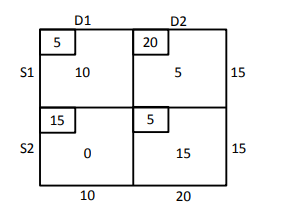
\includegraphics[width=0.75\columnwidth]{chapters/10/7/2/4/figs/fig.png}
 \end{center}
\caption{}
\label{fig:10/7/2/4Fig1}
\end{figure}
\fi

\item Find the position vector of the mid point of the vector joining the points $\vec{P}$(2, 3, 4)
and $\vec{Q}$(4, 1, –2).
\\
\solution
		\begin{enumerate}[label=\thesubsection.\arabic*,ref=\thesubsection.\theenumi]
\item Find the coordinates of the point which divides the join of $(-1,7) $ and $ (4,-3)$ in the ratio 2:3.
	\\
		\solution
	\input{chapters/10/7/2/1/section.tex}
\item Find the coordinates of the point $\vec{R}$ on the line segment joining the points $\vec{P}(-1,3)$ and $\vec{Q}(2,5)$ such that $PR=\frac{3}{5}PQ$.
\item Find the ratio in which the point $\vec{P}\brak{\frac{3}{4},\frac{5}{12}}$ divides the line segment joining the points $\vec{A}\brak{\frac{1}{2},\frac{3}{2}}$ and $ \vec{B}(2,-5)$.
\item Find the coordinates of the point which divides the line segment joining the points $(4,-3)$ and $(8,5)$ in the ratio $3:1$ internally.
\item Find the coordinates of the point $\vec{P}$ on $AD$ such that $AP : PD = 2 : 1$.
\item If the point $\vec{P} (2, 1)$ lies on the line segment joining points $\vec{A} (4, 2)$  and $ \vec{B} (8, 4)$,
then
\begin{enumerate}
	\item $AP =\frac{1}{3}{AB}$ 
\item ${AP}={PE}$
\item ${PB}=\frac{1}{3}{AB}$
\item${AP}=\frac{1}{2}{AB}$
 \end{enumerate}
\item Find the ratio in which the line segment joining the points $(-3,10)$  and  $(6,-8)$  is divided by $ (-1,6)$.
	\\
		\solution
	\input{chapters/10/7/2/4/section.tex}
\item Find the position vector of the mid point of the vector joining the points $\vec{P}$(2, 3, 4)
and $\vec{Q}$(4, 1, –2).
\\
\solution
		\input{chapters/12/10/2/16/section.tex}
\item Let $\vec{A}(4, 2), \vec{B}(6, 5)$  and $ \vec{C}(1, 4)$ be the vertices of $\triangle ABC$.
\begin{enumerate}
\item If $\vec{A}$ and  $\vec{B}$ are $(-2,-2)$ and  $(2,-4)$, respectively, find the coordinates of $\vec{P}$ such that $AP= \frac {3}{7}AB$  and $ \vec{P}$ lies on the line segment $AB$.
	\\
		\solution
	\input{chapters/10/7/2/8/section.tex}
\item Find the coordinates of the points which divide the line segment joining $A(-2,2)$  and  $\vec{B}(2,8)$ into four equal parts.
	\\
		\solution
	\input{chapters/10/7/2/9/section.tex}
\item In what ratio does the point $(-4,6)$ divide the line segment joining the points $\vec{A}(-6,0)$ and $\vec{B}(3,-8)$?
\item Given that $\vec{P}(3,2,-4), \vec{Q}(5,4,-6)$ and $\vec{R}(9,8,-10)$ are collinear. Find the ratio in which $\vec{Q}$ divides $PR$.
\item Points $\vec{A}(-6,10),\vec{B}(-4,6)$  and  $\vec{C}(3,-8)$ are collinear such that $AB=  \frac{2}{9}AC$.
\item The point which divides the line segment joining the points $\vec{P} (7, –6) $  and  $\vec{Q}(3, 4)$ in the 
ratio 1 : 2 internally lies in  which quadrant?
\item Find the coordinates of the points of trisection of the line segment joining $(4,-1)$  and  $(-2,3)$.
	\\
		\solution
	\input{chapters/10/7/2/2/section.tex}
\item Find the coordinates of the points which trisect the line segment joining the points $\vec{P}(4,2,-6)$ and $\vec{Q}(10,-16,6)$.
\item Find the coordinates of the points of trisection (i.e. points dividing to three equal parts) of the line segment joining the points $\vec{A}(2,-2)$ and $\vec{B}(-7,4)$.
\item Point $\vec{P}(5,-3)$ is one of the two points of trisection of line segment joining the points $\vec{A}(7,-2)$ and $\vec{B}(1,-5)$
\item Find the position vector of a point $\vec{R}$ which divides the line joining two points $\vec{P}$
and $\vec{Q}$ whose position vectors are $\hat{i}+2\hat{j}-\hat{k}$ and $-\hat{i}+\hat{j}+\hat{k}$ respectively, in the
ratio 2 : 1
\begin{enumerate}
    \item  internally
    \item  externally
\end{enumerate}
%\solution
%		\input{chapters/12/10/2/15/section.tex}
\item Find the coordinates of the point which divides the line segment joining the points which divides the line segment joining  the points $(-2,3,5)$ and $(1,-4,6)$ in the ratio 
\begin{enumerate}
\item $2:3$ internally,
\item $2:3$ externally
\end{enumerate}
\item Find the coordinates of the point which divides the line segment joining the points $(1,-2,3)$ and $(3,4,-5)$ in the ratio $2:3$
\begin{enumerate}
\item internally, and
\item externally
\end{enumerate}
\item Consider two points $\vec{P}$ and $\vec{Q}$ with position vectors $\overrightarrow{OP} = 3\overrightarrow{a}-2\overrightarrow{b}$ and $\overrightarrow{OQ}=\overrightarrow{a}+\overrightarrow{b}$. Find the position vector of a point $\vec{R}$ which divides the line joining $\vec{P}$ and $\vec{Q}$ in the ratio $2:1$, 
\begin{enumerate}
\item internally, and 
\item externally.
\end{enumerate}
\item The median from $\vec{A}$ meets $BC$ at $\vec{D}$. Find the coordinates of the point $\vec{D}$.
\item Find the coordinates of points $\vec{Q}$ and $\vec{R}$ on medians $BE$ and $CF$ respectively such that $BQ : QE = 2 : 1$  and  $CR : RF = 2 : 1$.
\item What do you observe?
\item If $\vec{A}, \vec{B}$ and $\vec{C}$  are the vertices of $\triangle ABC$, find the coordinates of the centroid of the triangle.
\end{enumerate}
\solution
	\input{chapters/10/7/4/7/section.tex}
\item If $\vec{P}(9a-2,-b)$ divides line segment joining $\vec{A}(3a+1,-3)$ and $\vec{B}(8a,5)$ in the ratio 3:1, find the values of $a$ and $b$.
\item Find the position vector of a point $\vec{R}$ which divides the line joining two points $\vec{P}$ and $\vec{Q}$ whose position vectors are $2\vec{a}+\vec{b}$ and $\vec{a}-3\vec{b}$ externally in the ratio $1:2$.
\item The position vector of the point which divides the join of points 2$\vec{a}$-3$\vec{b}$ $\text{and}$ $\vec{a}+\vec{b}$ in the ratio 3:1 is \rule{1cm}{0.1pt}.
\item If $\vec{a}$ and $\vec{b}$ are the postion vectors of $\vec{A}$ and $\vec{B}$, respectively, find the position vector of a point $\vec{C}$ in $BA$ produced such that $BC=1.5BA$.
\item Find the position vector of a point $\vec{R}$ which divides the line joining two points $\vec{P}$ and $\vec{Q}$ whose position vectors are $(2\vec{a}+\vec{b})$ and $(\vec{a}-3\vec{b})$
externally in the ratio 1 : 2. Also, show that $\vec{P}$ is the mid point of the line segment $RQ$.
\end{enumerate}

\item Let $\vec{A}(4, 2), \vec{B}(6, 5)$  and $ \vec{C}(1, 4)$ be the vertices of $\triangle ABC$.
\begin{enumerate}
\item If $\vec{A}$ and  $\vec{B}$ are $(-2,-2)$ and  $(2,-4)$, respectively, find the coordinates of $\vec{P}$ such that $AP= \frac {3}{7}AB$  and $ \vec{P}$ lies on the line segment $AB$.
	\\
		\solution
	\begin{enumerate}[label=\thesubsection.\arabic*,ref=\thesubsection.\theenumi]
\item Find the coordinates of the point which divides the join of $(-1,7) $ and $ (4,-3)$ in the ratio 2:3.
	\\
		\solution
	\input{chapters/10/7/2/1/section.tex}
\item Find the coordinates of the point $\vec{R}$ on the line segment joining the points $\vec{P}(-1,3)$ and $\vec{Q}(2,5)$ such that $PR=\frac{3}{5}PQ$.
\item Find the ratio in which the point $\vec{P}\brak{\frac{3}{4},\frac{5}{12}}$ divides the line segment joining the points $\vec{A}\brak{\frac{1}{2},\frac{3}{2}}$ and $ \vec{B}(2,-5)$.
\item Find the coordinates of the point which divides the line segment joining the points $(4,-3)$ and $(8,5)$ in the ratio $3:1$ internally.
\item Find the coordinates of the point $\vec{P}$ on $AD$ such that $AP : PD = 2 : 1$.
\item If the point $\vec{P} (2, 1)$ lies on the line segment joining points $\vec{A} (4, 2)$  and $ \vec{B} (8, 4)$,
then
\begin{enumerate}
	\item $AP =\frac{1}{3}{AB}$ 
\item ${AP}={PE}$
\item ${PB}=\frac{1}{3}{AB}$
\item${AP}=\frac{1}{2}{AB}$
 \end{enumerate}
\item Find the ratio in which the line segment joining the points $(-3,10)$  and  $(6,-8)$  is divided by $ (-1,6)$.
	\\
		\solution
	\input{chapters/10/7/2/4/section.tex}
\item Find the position vector of the mid point of the vector joining the points $\vec{P}$(2, 3, 4)
and $\vec{Q}$(4, 1, –2).
\\
\solution
		\input{chapters/12/10/2/16/section.tex}
\item Let $\vec{A}(4, 2), \vec{B}(6, 5)$  and $ \vec{C}(1, 4)$ be the vertices of $\triangle ABC$.
\begin{enumerate}
\item If $\vec{A}$ and  $\vec{B}$ are $(-2,-2)$ and  $(2,-4)$, respectively, find the coordinates of $\vec{P}$ such that $AP= \frac {3}{7}AB$  and $ \vec{P}$ lies on the line segment $AB$.
	\\
		\solution
	\input{chapters/10/7/2/8/section.tex}
\item Find the coordinates of the points which divide the line segment joining $A(-2,2)$  and  $\vec{B}(2,8)$ into four equal parts.
	\\
		\solution
	\input{chapters/10/7/2/9/section.tex}
\item In what ratio does the point $(-4,6)$ divide the line segment joining the points $\vec{A}(-6,0)$ and $\vec{B}(3,-8)$?
\item Given that $\vec{P}(3,2,-4), \vec{Q}(5,4,-6)$ and $\vec{R}(9,8,-10)$ are collinear. Find the ratio in which $\vec{Q}$ divides $PR$.
\item Points $\vec{A}(-6,10),\vec{B}(-4,6)$  and  $\vec{C}(3,-8)$ are collinear such that $AB=  \frac{2}{9}AC$.
\item The point which divides the line segment joining the points $\vec{P} (7, –6) $  and  $\vec{Q}(3, 4)$ in the 
ratio 1 : 2 internally lies in  which quadrant?
\item Find the coordinates of the points of trisection of the line segment joining $(4,-1)$  and  $(-2,3)$.
	\\
		\solution
	\input{chapters/10/7/2/2/section.tex}
\item Find the coordinates of the points which trisect the line segment joining the points $\vec{P}(4,2,-6)$ and $\vec{Q}(10,-16,6)$.
\item Find the coordinates of the points of trisection (i.e. points dividing to three equal parts) of the line segment joining the points $\vec{A}(2,-2)$ and $\vec{B}(-7,4)$.
\item Point $\vec{P}(5,-3)$ is one of the two points of trisection of line segment joining the points $\vec{A}(7,-2)$ and $\vec{B}(1,-5)$
\item Find the position vector of a point $\vec{R}$ which divides the line joining two points $\vec{P}$
and $\vec{Q}$ whose position vectors are $\hat{i}+2\hat{j}-\hat{k}$ and $-\hat{i}+\hat{j}+\hat{k}$ respectively, in the
ratio 2 : 1
\begin{enumerate}
    \item  internally
    \item  externally
\end{enumerate}
%\solution
%		\input{chapters/12/10/2/15/section.tex}
\item Find the coordinates of the point which divides the line segment joining the points which divides the line segment joining  the points $(-2,3,5)$ and $(1,-4,6)$ in the ratio 
\begin{enumerate}
\item $2:3$ internally,
\item $2:3$ externally
\end{enumerate}
\item Find the coordinates of the point which divides the line segment joining the points $(1,-2,3)$ and $(3,4,-5)$ in the ratio $2:3$
\begin{enumerate}
\item internally, and
\item externally
\end{enumerate}
\item Consider two points $\vec{P}$ and $\vec{Q}$ with position vectors $\overrightarrow{OP} = 3\overrightarrow{a}-2\overrightarrow{b}$ and $\overrightarrow{OQ}=\overrightarrow{a}+\overrightarrow{b}$. Find the position vector of a point $\vec{R}$ which divides the line joining $\vec{P}$ and $\vec{Q}$ in the ratio $2:1$, 
\begin{enumerate}
\item internally, and 
\item externally.
\end{enumerate}
\item The median from $\vec{A}$ meets $BC$ at $\vec{D}$. Find the coordinates of the point $\vec{D}$.
\item Find the coordinates of points $\vec{Q}$ and $\vec{R}$ on medians $BE$ and $CF$ respectively such that $BQ : QE = 2 : 1$  and  $CR : RF = 2 : 1$.
\item What do you observe?
\item If $\vec{A}, \vec{B}$ and $\vec{C}$  are the vertices of $\triangle ABC$, find the coordinates of the centroid of the triangle.
\end{enumerate}
\solution
	\input{chapters/10/7/4/7/section.tex}
\item If $\vec{P}(9a-2,-b)$ divides line segment joining $\vec{A}(3a+1,-3)$ and $\vec{B}(8a,5)$ in the ratio 3:1, find the values of $a$ and $b$.
\item Find the position vector of a point $\vec{R}$ which divides the line joining two points $\vec{P}$ and $\vec{Q}$ whose position vectors are $2\vec{a}+\vec{b}$ and $\vec{a}-3\vec{b}$ externally in the ratio $1:2$.
\item The position vector of the point which divides the join of points 2$\vec{a}$-3$\vec{b}$ $\text{and}$ $\vec{a}+\vec{b}$ in the ratio 3:1 is \rule{1cm}{0.1pt}.
\item If $\vec{a}$ and $\vec{b}$ are the postion vectors of $\vec{A}$ and $\vec{B}$, respectively, find the position vector of a point $\vec{C}$ in $BA$ produced such that $BC=1.5BA$.
\item Find the position vector of a point $\vec{R}$ which divides the line joining two points $\vec{P}$ and $\vec{Q}$ whose position vectors are $(2\vec{a}+\vec{b})$ and $(\vec{a}-3\vec{b})$
externally in the ratio 1 : 2. Also, show that $\vec{P}$ is the mid point of the line segment $RQ$.
\end{enumerate}

\item Find the coordinates of the points which divide the line segment joining $A(-2,2)$  and  $\vec{B}(2,8)$ into four equal parts.
	\\
		\solution
	\begin{enumerate}[label=\thesubsection.\arabic*,ref=\thesubsection.\theenumi]
\item Find the coordinates of the point which divides the join of $(-1,7) $ and $ (4,-3)$ in the ratio 2:3.
	\\
		\solution
	\input{chapters/10/7/2/1/section.tex}
\item Find the coordinates of the point $\vec{R}$ on the line segment joining the points $\vec{P}(-1,3)$ and $\vec{Q}(2,5)$ such that $PR=\frac{3}{5}PQ$.
\item Find the ratio in which the point $\vec{P}\brak{\frac{3}{4},\frac{5}{12}}$ divides the line segment joining the points $\vec{A}\brak{\frac{1}{2},\frac{3}{2}}$ and $ \vec{B}(2,-5)$.
\item Find the coordinates of the point which divides the line segment joining the points $(4,-3)$ and $(8,5)$ in the ratio $3:1$ internally.
\item Find the coordinates of the point $\vec{P}$ on $AD$ such that $AP : PD = 2 : 1$.
\item If the point $\vec{P} (2, 1)$ lies on the line segment joining points $\vec{A} (4, 2)$  and $ \vec{B} (8, 4)$,
then
\begin{enumerate}
	\item $AP =\frac{1}{3}{AB}$ 
\item ${AP}={PE}$
\item ${PB}=\frac{1}{3}{AB}$
\item${AP}=\frac{1}{2}{AB}$
 \end{enumerate}
\item Find the ratio in which the line segment joining the points $(-3,10)$  and  $(6,-8)$  is divided by $ (-1,6)$.
	\\
		\solution
	\input{chapters/10/7/2/4/section.tex}
\item Find the position vector of the mid point of the vector joining the points $\vec{P}$(2, 3, 4)
and $\vec{Q}$(4, 1, –2).
\\
\solution
		\input{chapters/12/10/2/16/section.tex}
\item Let $\vec{A}(4, 2), \vec{B}(6, 5)$  and $ \vec{C}(1, 4)$ be the vertices of $\triangle ABC$.
\begin{enumerate}
\item If $\vec{A}$ and  $\vec{B}$ are $(-2,-2)$ and  $(2,-4)$, respectively, find the coordinates of $\vec{P}$ such that $AP= \frac {3}{7}AB$  and $ \vec{P}$ lies on the line segment $AB$.
	\\
		\solution
	\input{chapters/10/7/2/8/section.tex}
\item Find the coordinates of the points which divide the line segment joining $A(-2,2)$  and  $\vec{B}(2,8)$ into four equal parts.
	\\
		\solution
	\input{chapters/10/7/2/9/section.tex}
\item In what ratio does the point $(-4,6)$ divide the line segment joining the points $\vec{A}(-6,0)$ and $\vec{B}(3,-8)$?
\item Given that $\vec{P}(3,2,-4), \vec{Q}(5,4,-6)$ and $\vec{R}(9,8,-10)$ are collinear. Find the ratio in which $\vec{Q}$ divides $PR$.
\item Points $\vec{A}(-6,10),\vec{B}(-4,6)$  and  $\vec{C}(3,-8)$ are collinear such that $AB=  \frac{2}{9}AC$.
\item The point which divides the line segment joining the points $\vec{P} (7, –6) $  and  $\vec{Q}(3, 4)$ in the 
ratio 1 : 2 internally lies in  which quadrant?
\item Find the coordinates of the points of trisection of the line segment joining $(4,-1)$  and  $(-2,3)$.
	\\
		\solution
	\input{chapters/10/7/2/2/section.tex}
\item Find the coordinates of the points which trisect the line segment joining the points $\vec{P}(4,2,-6)$ and $\vec{Q}(10,-16,6)$.
\item Find the coordinates of the points of trisection (i.e. points dividing to three equal parts) of the line segment joining the points $\vec{A}(2,-2)$ and $\vec{B}(-7,4)$.
\item Point $\vec{P}(5,-3)$ is one of the two points of trisection of line segment joining the points $\vec{A}(7,-2)$ and $\vec{B}(1,-5)$
\item Find the position vector of a point $\vec{R}$ which divides the line joining two points $\vec{P}$
and $\vec{Q}$ whose position vectors are $\hat{i}+2\hat{j}-\hat{k}$ and $-\hat{i}+\hat{j}+\hat{k}$ respectively, in the
ratio 2 : 1
\begin{enumerate}
    \item  internally
    \item  externally
\end{enumerate}
%\solution
%		\input{chapters/12/10/2/15/section.tex}
\item Find the coordinates of the point which divides the line segment joining the points which divides the line segment joining  the points $(-2,3,5)$ and $(1,-4,6)$ in the ratio 
\begin{enumerate}
\item $2:3$ internally,
\item $2:3$ externally
\end{enumerate}
\item Find the coordinates of the point which divides the line segment joining the points $(1,-2,3)$ and $(3,4,-5)$ in the ratio $2:3$
\begin{enumerate}
\item internally, and
\item externally
\end{enumerate}
\item Consider two points $\vec{P}$ and $\vec{Q}$ with position vectors $\overrightarrow{OP} = 3\overrightarrow{a}-2\overrightarrow{b}$ and $\overrightarrow{OQ}=\overrightarrow{a}+\overrightarrow{b}$. Find the position vector of a point $\vec{R}$ which divides the line joining $\vec{P}$ and $\vec{Q}$ in the ratio $2:1$, 
\begin{enumerate}
\item internally, and 
\item externally.
\end{enumerate}
\item The median from $\vec{A}$ meets $BC$ at $\vec{D}$. Find the coordinates of the point $\vec{D}$.
\item Find the coordinates of points $\vec{Q}$ and $\vec{R}$ on medians $BE$ and $CF$ respectively such that $BQ : QE = 2 : 1$  and  $CR : RF = 2 : 1$.
\item What do you observe?
\item If $\vec{A}, \vec{B}$ and $\vec{C}$  are the vertices of $\triangle ABC$, find the coordinates of the centroid of the triangle.
\end{enumerate}
\solution
	\input{chapters/10/7/4/7/section.tex}
\item If $\vec{P}(9a-2,-b)$ divides line segment joining $\vec{A}(3a+1,-3)$ and $\vec{B}(8a,5)$ in the ratio 3:1, find the values of $a$ and $b$.
\item Find the position vector of a point $\vec{R}$ which divides the line joining two points $\vec{P}$ and $\vec{Q}$ whose position vectors are $2\vec{a}+\vec{b}$ and $\vec{a}-3\vec{b}$ externally in the ratio $1:2$.
\item The position vector of the point which divides the join of points 2$\vec{a}$-3$\vec{b}$ $\text{and}$ $\vec{a}+\vec{b}$ in the ratio 3:1 is \rule{1cm}{0.1pt}.
\item If $\vec{a}$ and $\vec{b}$ are the postion vectors of $\vec{A}$ and $\vec{B}$, respectively, find the position vector of a point $\vec{C}$ in $BA$ produced such that $BC=1.5BA$.
\item Find the position vector of a point $\vec{R}$ which divides the line joining two points $\vec{P}$ and $\vec{Q}$ whose position vectors are $(2\vec{a}+\vec{b})$ and $(\vec{a}-3\vec{b})$
externally in the ratio 1 : 2. Also, show that $\vec{P}$ is the mid point of the line segment $RQ$.
\end{enumerate}

\item In what ratio does the point $(-4,6)$ divide the line segment joining the points $\vec{A}(-6,0)$ and $\vec{B}(3,-8)$?
\item Given that $\vec{P}(3,2,-4), \vec{Q}(5,4,-6)$ and $\vec{R}(9,8,-10)$ are collinear. Find the ratio in which $\vec{Q}$ divides $PR$.
\item Points $\vec{A}(-6,10),\vec{B}(-4,6)$  and  $\vec{C}(3,-8)$ are collinear such that $AB=  \frac{2}{9}AC$.
\item The point which divides the line segment joining the points $\vec{P} (7, –6) $  and  $\vec{Q}(3, 4)$ in the 
ratio 1 : 2 internally lies in  which quadrant?
\item Find the coordinates of the points of trisection of the line segment joining $(4,-1)$  and  $(-2,3)$.
	\\
		\solution
	Using section formula,
\begin{align}
\vec{R}=\frac{1}{1+\frac{1}{2}}\brak{\myvec{4\\-1}+\frac{1}{2}\myvec{-2\\3}}
=\myvec{2\\ \frac{1}{3}}\\
\vec{S}=\frac{1}{1+\frac{2}{1}}\brak{\myvec{4\\-1}+\frac{2}{1}\myvec{-2\\3}}
=\myvec{0\\ \frac{5}{3}}
\end{align}
which are the desired points of trisection.
\iffalse
See
		\figref{fig:chapters/10/7/2/2/Figure}
\begin{figure}[H]
\centering
\includegraphics[width=0.75\columnwidth]{chapters/10/7/2/2/figs/dj.pdf}
\caption{}
		\label{fig:chapters/10/7/2/2/Figure}
\end{figure}
\fi

\item Find the coordinates of the points which trisect the line segment joining the points $\vec{P}(4,2,-6)$ and $\vec{Q}(10,-16,6)$.
\item Find the coordinates of the points of trisection (i.e. points dividing to three equal parts) of the line segment joining the points $\vec{A}(2,-2)$ and $\vec{B}(-7,4)$.
\item Point $\vec{P}(5,-3)$ is one of the two points of trisection of line segment joining the points $\vec{A}(7,-2)$ and $\vec{B}(1,-5)$
\item Find the position vector of a point $\vec{R}$ which divides the line joining two points $\vec{P}$
and $\vec{Q}$ whose position vectors are $\hat{i}+2\hat{j}-\hat{k}$ and $-\hat{i}+\hat{j}+\hat{k}$ respectively, in the
ratio 2 : 1
\begin{enumerate}
    \item  internally
    \item  externally
\end{enumerate}
%\solution
%		\begin{enumerate}[label=\thesubsection.\arabic*,ref=\thesubsection.\theenumi]
\item Find the coordinates of the point which divides the join of $(-1,7) $ and $ (4,-3)$ in the ratio 2:3.
	\\
		\solution
	\input{chapters/10/7/2/1/section.tex}
\item Find the coordinates of the point $\vec{R}$ on the line segment joining the points $\vec{P}(-1,3)$ and $\vec{Q}(2,5)$ such that $PR=\frac{3}{5}PQ$.
\item Find the ratio in which the point $\vec{P}\brak{\frac{3}{4},\frac{5}{12}}$ divides the line segment joining the points $\vec{A}\brak{\frac{1}{2},\frac{3}{2}}$ and $ \vec{B}(2,-5)$.
\item Find the coordinates of the point which divides the line segment joining the points $(4,-3)$ and $(8,5)$ in the ratio $3:1$ internally.
\item Find the coordinates of the point $\vec{P}$ on $AD$ such that $AP : PD = 2 : 1$.
\item If the point $\vec{P} (2, 1)$ lies on the line segment joining points $\vec{A} (4, 2)$  and $ \vec{B} (8, 4)$,
then
\begin{enumerate}
	\item $AP =\frac{1}{3}{AB}$ 
\item ${AP}={PE}$
\item ${PB}=\frac{1}{3}{AB}$
\item${AP}=\frac{1}{2}{AB}$
 \end{enumerate}
\item Find the ratio in which the line segment joining the points $(-3,10)$  and  $(6,-8)$  is divided by $ (-1,6)$.
	\\
		\solution
	\input{chapters/10/7/2/4/section.tex}
\item Find the position vector of the mid point of the vector joining the points $\vec{P}$(2, 3, 4)
and $\vec{Q}$(4, 1, –2).
\\
\solution
		\input{chapters/12/10/2/16/section.tex}
\item Let $\vec{A}(4, 2), \vec{B}(6, 5)$  and $ \vec{C}(1, 4)$ be the vertices of $\triangle ABC$.
\begin{enumerate}
\item If $\vec{A}$ and  $\vec{B}$ are $(-2,-2)$ and  $(2,-4)$, respectively, find the coordinates of $\vec{P}$ such that $AP= \frac {3}{7}AB$  and $ \vec{P}$ lies on the line segment $AB$.
	\\
		\solution
	\input{chapters/10/7/2/8/section.tex}
\item Find the coordinates of the points which divide the line segment joining $A(-2,2)$  and  $\vec{B}(2,8)$ into four equal parts.
	\\
		\solution
	\input{chapters/10/7/2/9/section.tex}
\item In what ratio does the point $(-4,6)$ divide the line segment joining the points $\vec{A}(-6,0)$ and $\vec{B}(3,-8)$?
\item Given that $\vec{P}(3,2,-4), \vec{Q}(5,4,-6)$ and $\vec{R}(9,8,-10)$ are collinear. Find the ratio in which $\vec{Q}$ divides $PR$.
\item Points $\vec{A}(-6,10),\vec{B}(-4,6)$  and  $\vec{C}(3,-8)$ are collinear such that $AB=  \frac{2}{9}AC$.
\item The point which divides the line segment joining the points $\vec{P} (7, –6) $  and  $\vec{Q}(3, 4)$ in the 
ratio 1 : 2 internally lies in  which quadrant?
\item Find the coordinates of the points of trisection of the line segment joining $(4,-1)$  and  $(-2,3)$.
	\\
		\solution
	\input{chapters/10/7/2/2/section.tex}
\item Find the coordinates of the points which trisect the line segment joining the points $\vec{P}(4,2,-6)$ and $\vec{Q}(10,-16,6)$.
\item Find the coordinates of the points of trisection (i.e. points dividing to three equal parts) of the line segment joining the points $\vec{A}(2,-2)$ and $\vec{B}(-7,4)$.
\item Point $\vec{P}(5,-3)$ is one of the two points of trisection of line segment joining the points $\vec{A}(7,-2)$ and $\vec{B}(1,-5)$
\item Find the position vector of a point $\vec{R}$ which divides the line joining two points $\vec{P}$
and $\vec{Q}$ whose position vectors are $\hat{i}+2\hat{j}-\hat{k}$ and $-\hat{i}+\hat{j}+\hat{k}$ respectively, in the
ratio 2 : 1
\begin{enumerate}
    \item  internally
    \item  externally
\end{enumerate}
%\solution
%		\input{chapters/12/10/2/15/section.tex}
\item Find the coordinates of the point which divides the line segment joining the points which divides the line segment joining  the points $(-2,3,5)$ and $(1,-4,6)$ in the ratio 
\begin{enumerate}
\item $2:3$ internally,
\item $2:3$ externally
\end{enumerate}
\item Find the coordinates of the point which divides the line segment joining the points $(1,-2,3)$ and $(3,4,-5)$ in the ratio $2:3$
\begin{enumerate}
\item internally, and
\item externally
\end{enumerate}
\item Consider two points $\vec{P}$ and $\vec{Q}$ with position vectors $\overrightarrow{OP} = 3\overrightarrow{a}-2\overrightarrow{b}$ and $\overrightarrow{OQ}=\overrightarrow{a}+\overrightarrow{b}$. Find the position vector of a point $\vec{R}$ which divides the line joining $\vec{P}$ and $\vec{Q}$ in the ratio $2:1$, 
\begin{enumerate}
\item internally, and 
\item externally.
\end{enumerate}
\item The median from $\vec{A}$ meets $BC$ at $\vec{D}$. Find the coordinates of the point $\vec{D}$.
\item Find the coordinates of points $\vec{Q}$ and $\vec{R}$ on medians $BE$ and $CF$ respectively such that $BQ : QE = 2 : 1$  and  $CR : RF = 2 : 1$.
\item What do you observe?
\item If $\vec{A}, \vec{B}$ and $\vec{C}$  are the vertices of $\triangle ABC$, find the coordinates of the centroid of the triangle.
\end{enumerate}
\solution
	\input{chapters/10/7/4/7/section.tex}
\item If $\vec{P}(9a-2,-b)$ divides line segment joining $\vec{A}(3a+1,-3)$ and $\vec{B}(8a,5)$ in the ratio 3:1, find the values of $a$ and $b$.
\item Find the position vector of a point $\vec{R}$ which divides the line joining two points $\vec{P}$ and $\vec{Q}$ whose position vectors are $2\vec{a}+\vec{b}$ and $\vec{a}-3\vec{b}$ externally in the ratio $1:2$.
\item The position vector of the point which divides the join of points 2$\vec{a}$-3$\vec{b}$ $\text{and}$ $\vec{a}+\vec{b}$ in the ratio 3:1 is \rule{1cm}{0.1pt}.
\item If $\vec{a}$ and $\vec{b}$ are the postion vectors of $\vec{A}$ and $\vec{B}$, respectively, find the position vector of a point $\vec{C}$ in $BA$ produced such that $BC=1.5BA$.
\item Find the position vector of a point $\vec{R}$ which divides the line joining two points $\vec{P}$ and $\vec{Q}$ whose position vectors are $(2\vec{a}+\vec{b})$ and $(\vec{a}-3\vec{b})$
externally in the ratio 1 : 2. Also, show that $\vec{P}$ is the mid point of the line segment $RQ$.
\end{enumerate}

\item Find the coordinates of the point which divides the line segment joining the points which divides the line segment joining  the points $(-2,3,5)$ and $(1,-4,6)$ in the ratio 
\begin{enumerate}
\item $2:3$ internally,
\item $2:3$ externally
\end{enumerate}
\item Find the coordinates of the point which divides the line segment joining the points $(1,-2,3)$ and $(3,4,-5)$ in the ratio $2:3$
\begin{enumerate}
\item internally, and
\item externally
\end{enumerate}
\item Consider two points $\vec{P}$ and $\vec{Q}$ with position vectors $\overrightarrow{OP} = 3\overrightarrow{a}-2\overrightarrow{b}$ and $\overrightarrow{OQ}=\overrightarrow{a}+\overrightarrow{b}$. Find the position vector of a point $\vec{R}$ which divides the line joining $\vec{P}$ and $\vec{Q}$ in the ratio $2:1$, 
\begin{enumerate}
\item internally, and 
\item externally.
\end{enumerate}
\item The median from $\vec{A}$ meets $BC$ at $\vec{D}$. Find the coordinates of the point $\vec{D}$.
\item Find the coordinates of points $\vec{Q}$ and $\vec{R}$ on medians $BE$ and $CF$ respectively such that $BQ : QE = 2 : 1$  and  $CR : RF = 2 : 1$.
\item What do you observe?
\item If $\vec{A}, \vec{B}$ and $\vec{C}$  are the vertices of $\triangle ABC$, find the coordinates of the centroid of the triangle.
\end{enumerate}
\solution
	\begin{enumerate}[label=\thesubsection.\arabic*,ref=\thesubsection.\theenumi]
\item Find the coordinates of the point which divides the join of $(-1,7) $ and $ (4,-3)$ in the ratio 2:3.
	\\
		\solution
	\input{chapters/10/7/2/1/section.tex}
\item Find the coordinates of the point $\vec{R}$ on the line segment joining the points $\vec{P}(-1,3)$ and $\vec{Q}(2,5)$ such that $PR=\frac{3}{5}PQ$.
\item Find the ratio in which the point $\vec{P}\brak{\frac{3}{4},\frac{5}{12}}$ divides the line segment joining the points $\vec{A}\brak{\frac{1}{2},\frac{3}{2}}$ and $ \vec{B}(2,-5)$.
\item Find the coordinates of the point which divides the line segment joining the points $(4,-3)$ and $(8,5)$ in the ratio $3:1$ internally.
\item Find the coordinates of the point $\vec{P}$ on $AD$ such that $AP : PD = 2 : 1$.
\item If the point $\vec{P} (2, 1)$ lies on the line segment joining points $\vec{A} (4, 2)$  and $ \vec{B} (8, 4)$,
then
\begin{enumerate}
	\item $AP =\frac{1}{3}{AB}$ 
\item ${AP}={PE}$
\item ${PB}=\frac{1}{3}{AB}$
\item${AP}=\frac{1}{2}{AB}$
 \end{enumerate}
\item Find the ratio in which the line segment joining the points $(-3,10)$  and  $(6,-8)$  is divided by $ (-1,6)$.
	\\
		\solution
	\input{chapters/10/7/2/4/section.tex}
\item Find the position vector of the mid point of the vector joining the points $\vec{P}$(2, 3, 4)
and $\vec{Q}$(4, 1, –2).
\\
\solution
		\input{chapters/12/10/2/16/section.tex}
\item Let $\vec{A}(4, 2), \vec{B}(6, 5)$  and $ \vec{C}(1, 4)$ be the vertices of $\triangle ABC$.
\begin{enumerate}
\item If $\vec{A}$ and  $\vec{B}$ are $(-2,-2)$ and  $(2,-4)$, respectively, find the coordinates of $\vec{P}$ such that $AP= \frac {3}{7}AB$  and $ \vec{P}$ lies on the line segment $AB$.
	\\
		\solution
	\input{chapters/10/7/2/8/section.tex}
\item Find the coordinates of the points which divide the line segment joining $A(-2,2)$  and  $\vec{B}(2,8)$ into four equal parts.
	\\
		\solution
	\input{chapters/10/7/2/9/section.tex}
\item In what ratio does the point $(-4,6)$ divide the line segment joining the points $\vec{A}(-6,0)$ and $\vec{B}(3,-8)$?
\item Given that $\vec{P}(3,2,-4), \vec{Q}(5,4,-6)$ and $\vec{R}(9,8,-10)$ are collinear. Find the ratio in which $\vec{Q}$ divides $PR$.
\item Points $\vec{A}(-6,10),\vec{B}(-4,6)$  and  $\vec{C}(3,-8)$ are collinear such that $AB=  \frac{2}{9}AC$.
\item The point which divides the line segment joining the points $\vec{P} (7, –6) $  and  $\vec{Q}(3, 4)$ in the 
ratio 1 : 2 internally lies in  which quadrant?
\item Find the coordinates of the points of trisection of the line segment joining $(4,-1)$  and  $(-2,3)$.
	\\
		\solution
	\input{chapters/10/7/2/2/section.tex}
\item Find the coordinates of the points which trisect the line segment joining the points $\vec{P}(4,2,-6)$ and $\vec{Q}(10,-16,6)$.
\item Find the coordinates of the points of trisection (i.e. points dividing to three equal parts) of the line segment joining the points $\vec{A}(2,-2)$ and $\vec{B}(-7,4)$.
\item Point $\vec{P}(5,-3)$ is one of the two points of trisection of line segment joining the points $\vec{A}(7,-2)$ and $\vec{B}(1,-5)$
\item Find the position vector of a point $\vec{R}$ which divides the line joining two points $\vec{P}$
and $\vec{Q}$ whose position vectors are $\hat{i}+2\hat{j}-\hat{k}$ and $-\hat{i}+\hat{j}+\hat{k}$ respectively, in the
ratio 2 : 1
\begin{enumerate}
    \item  internally
    \item  externally
\end{enumerate}
%\solution
%		\input{chapters/12/10/2/15/section.tex}
\item Find the coordinates of the point which divides the line segment joining the points which divides the line segment joining  the points $(-2,3,5)$ and $(1,-4,6)$ in the ratio 
\begin{enumerate}
\item $2:3$ internally,
\item $2:3$ externally
\end{enumerate}
\item Find the coordinates of the point which divides the line segment joining the points $(1,-2,3)$ and $(3,4,-5)$ in the ratio $2:3$
\begin{enumerate}
\item internally, and
\item externally
\end{enumerate}
\item Consider two points $\vec{P}$ and $\vec{Q}$ with position vectors $\overrightarrow{OP} = 3\overrightarrow{a}-2\overrightarrow{b}$ and $\overrightarrow{OQ}=\overrightarrow{a}+\overrightarrow{b}$. Find the position vector of a point $\vec{R}$ which divides the line joining $\vec{P}$ and $\vec{Q}$ in the ratio $2:1$, 
\begin{enumerate}
\item internally, and 
\item externally.
\end{enumerate}
\item The median from $\vec{A}$ meets $BC$ at $\vec{D}$. Find the coordinates of the point $\vec{D}$.
\item Find the coordinates of points $\vec{Q}$ and $\vec{R}$ on medians $BE$ and $CF$ respectively such that $BQ : QE = 2 : 1$  and  $CR : RF = 2 : 1$.
\item What do you observe?
\item If $\vec{A}, \vec{B}$ and $\vec{C}$  are the vertices of $\triangle ABC$, find the coordinates of the centroid of the triangle.
\end{enumerate}
\solution
	\input{chapters/10/7/4/7/section.tex}
\item If $\vec{P}(9a-2,-b)$ divides line segment joining $\vec{A}(3a+1,-3)$ and $\vec{B}(8a,5)$ in the ratio 3:1, find the values of $a$ and $b$.
\item Find the position vector of a point $\vec{R}$ which divides the line joining two points $\vec{P}$ and $\vec{Q}$ whose position vectors are $2\vec{a}+\vec{b}$ and $\vec{a}-3\vec{b}$ externally in the ratio $1:2$.
\item The position vector of the point which divides the join of points 2$\vec{a}$-3$\vec{b}$ $\text{and}$ $\vec{a}+\vec{b}$ in the ratio 3:1 is \rule{1cm}{0.1pt}.
\item If $\vec{a}$ and $\vec{b}$ are the postion vectors of $\vec{A}$ and $\vec{B}$, respectively, find the position vector of a point $\vec{C}$ in $BA$ produced such that $BC=1.5BA$.
\item Find the position vector of a point $\vec{R}$ which divides the line joining two points $\vec{P}$ and $\vec{Q}$ whose position vectors are $(2\vec{a}+\vec{b})$ and $(\vec{a}-3\vec{b})$
externally in the ratio 1 : 2. Also, show that $\vec{P}$ is the mid point of the line segment $RQ$.
\end{enumerate}

\item If $\vec{P}(9a-2,-b)$ divides line segment joining $\vec{A}(3a+1,-3)$ and $\vec{B}(8a,5)$ in the ratio 3:1, find the values of $a$ and $b$.
\item Find the position vector of a point $\vec{R}$ which divides the line joining two points $\vec{P}$ and $\vec{Q}$ whose position vectors are $2\vec{a}+\vec{b}$ and $\vec{a}-3\vec{b}$ externally in the ratio $1:2$.
\item The position vector of the point which divides the join of points 2$\vec{a}$-3$\vec{b}$ $\text{and}$ $\vec{a}+\vec{b}$ in the ratio 3:1 is \rule{1cm}{0.1pt}.
\item If $\vec{a}$ and $\vec{b}$ are the postion vectors of $\vec{A}$ and $\vec{B}$, respectively, find the position vector of a point $\vec{C}$ in $BA$ produced such that $BC=1.5BA$.
\item Find the position vector of a point $\vec{R}$ which divides the line joining two points $\vec{P}$ and $\vec{Q}$ whose position vectors are $(2\vec{a}+\vec{b})$ and $(\vec{a}-3\vec{b})$
externally in the ratio 1 : 2. Also, show that $\vec{P}$ is the mid point of the line segment $RQ$.
\end{enumerate}

\item Find the coordinates of the point $\vec{R}$ on the line segment joining the points $\vec{P}(-1,3)$ and $\vec{Q}(2,5)$ such that $PR=\frac{3}{5}PQ$.
\item Find the ratio in which the point $\vec{P}\brak{\frac{3}{4},\frac{5}{12}}$ divides the line segment joining the points $\vec{A}\brak{\frac{1}{2},\frac{3}{2}}$ and $ \vec{B}(2,-5)$.
\item Find the coordinates of the point which divides the line segment joining the points $(4,-3)$ and $(8,5)$ in the ratio $3:1$ internally.
\item Find the coordinates of the point $\vec{P}$ on $AD$ such that $AP : PD = 2 : 1$.
\item If the point $\vec{P} (2, 1)$ lies on the line segment joining points $\vec{A} (4, 2)$  and $ \vec{B} (8, 4)$,
then
\begin{enumerate}
	\item $AP =\frac{1}{3}{AB}$ 
\item ${AP}={PE}$
\item ${PB}=\frac{1}{3}{AB}$
\item${AP}=\frac{1}{2}{AB}$
 \end{enumerate}
\item Find the ratio in which the line segment joining the points $(-3,10)$  and  $(6,-8)$  is divided by $ (-1,6)$.
	\\
		\solution
	\iffalse
Using section formula,
\begin{align}
         \myvec{-1\\6} &=\frac{{\myvec{-3\\10}+k\myvec{6\\-8}}}{1+k}\\
	 \implies 7k\myvec{1 \\ -2} &= 2\myvec{1 \\ -2}
	 \\
	 \text{or, } k &= \frac{2}{7}.
\end{align}
\fi
In 
			\eqref{eq:section_formula-k}, substituting
			\begin{align}
				\vec{B} &= \myvec{-3\\10}, \vec{C} = \myvec{6\\-8}, \vec{D} = \myvec{-1\\6},
				\\
				k &= \frac{\myvec{-2 & 4}\myvec{-7 \\ 14}}{\norm{\myvec{-7 \\ 14}}^2} = \frac{2}{7}
			\end{align}
\iffalse
See \figref{fig:10/7/2/4Fig1}.
\begin{figure}[H]
 \begin{center}
  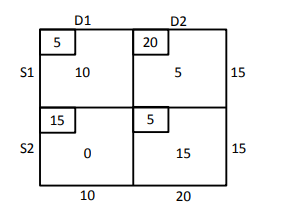
\includegraphics[width=0.75\columnwidth]{chapters/10/7/2/4/figs/fig.png}
 \end{center}
\caption{}
\label{fig:10/7/2/4Fig1}
\end{figure}
\fi

\item Find the position vector of the mid point of the vector joining the points $\vec{P}$(2, 3, 4)
and $\vec{Q}$(4, 1, –2).
\\
\solution
		\begin{enumerate}[label=\thesubsection.\arabic*,ref=\thesubsection.\theenumi]
\item Find the coordinates of the point which divides the join of $(-1,7) $ and $ (4,-3)$ in the ratio 2:3.
	\\
		\solution
	\begin{enumerate}[label=\thesubsection.\arabic*,ref=\thesubsection.\theenumi]
\item Find the coordinates of the point which divides the join of $(-1,7) $ and $ (4,-3)$ in the ratio 2:3.
	\\
		\solution
	\input{chapters/10/7/2/1/section.tex}
\item Find the coordinates of the point $\vec{R}$ on the line segment joining the points $\vec{P}(-1,3)$ and $\vec{Q}(2,5)$ such that $PR=\frac{3}{5}PQ$.
\item Find the ratio in which the point $\vec{P}\brak{\frac{3}{4},\frac{5}{12}}$ divides the line segment joining the points $\vec{A}\brak{\frac{1}{2},\frac{3}{2}}$ and $ \vec{B}(2,-5)$.
\item Find the coordinates of the point which divides the line segment joining the points $(4,-3)$ and $(8,5)$ in the ratio $3:1$ internally.
\item Find the coordinates of the point $\vec{P}$ on $AD$ such that $AP : PD = 2 : 1$.
\item If the point $\vec{P} (2, 1)$ lies on the line segment joining points $\vec{A} (4, 2)$  and $ \vec{B} (8, 4)$,
then
\begin{enumerate}
	\item $AP =\frac{1}{3}{AB}$ 
\item ${AP}={PE}$
\item ${PB}=\frac{1}{3}{AB}$
\item${AP}=\frac{1}{2}{AB}$
 \end{enumerate}
\item Find the ratio in which the line segment joining the points $(-3,10)$  and  $(6,-8)$  is divided by $ (-1,6)$.
	\\
		\solution
	\input{chapters/10/7/2/4/section.tex}
\item Find the position vector of the mid point of the vector joining the points $\vec{P}$(2, 3, 4)
and $\vec{Q}$(4, 1, –2).
\\
\solution
		\input{chapters/12/10/2/16/section.tex}
\item Let $\vec{A}(4, 2), \vec{B}(6, 5)$  and $ \vec{C}(1, 4)$ be the vertices of $\triangle ABC$.
\begin{enumerate}
\item If $\vec{A}$ and  $\vec{B}$ are $(-2,-2)$ and  $(2,-4)$, respectively, find the coordinates of $\vec{P}$ such that $AP= \frac {3}{7}AB$  and $ \vec{P}$ lies on the line segment $AB$.
	\\
		\solution
	\input{chapters/10/7/2/8/section.tex}
\item Find the coordinates of the points which divide the line segment joining $A(-2,2)$  and  $\vec{B}(2,8)$ into four equal parts.
	\\
		\solution
	\input{chapters/10/7/2/9/section.tex}
\item In what ratio does the point $(-4,6)$ divide the line segment joining the points $\vec{A}(-6,0)$ and $\vec{B}(3,-8)$?
\item Given that $\vec{P}(3,2,-4), \vec{Q}(5,4,-6)$ and $\vec{R}(9,8,-10)$ are collinear. Find the ratio in which $\vec{Q}$ divides $PR$.
\item Points $\vec{A}(-6,10),\vec{B}(-4,6)$  and  $\vec{C}(3,-8)$ are collinear such that $AB=  \frac{2}{9}AC$.
\item The point which divides the line segment joining the points $\vec{P} (7, –6) $  and  $\vec{Q}(3, 4)$ in the 
ratio 1 : 2 internally lies in  which quadrant?
\item Find the coordinates of the points of trisection of the line segment joining $(4,-1)$  and  $(-2,3)$.
	\\
		\solution
	\input{chapters/10/7/2/2/section.tex}
\item Find the coordinates of the points which trisect the line segment joining the points $\vec{P}(4,2,-6)$ and $\vec{Q}(10,-16,6)$.
\item Find the coordinates of the points of trisection (i.e. points dividing to three equal parts) of the line segment joining the points $\vec{A}(2,-2)$ and $\vec{B}(-7,4)$.
\item Point $\vec{P}(5,-3)$ is one of the two points of trisection of line segment joining the points $\vec{A}(7,-2)$ and $\vec{B}(1,-5)$
\item Find the position vector of a point $\vec{R}$ which divides the line joining two points $\vec{P}$
and $\vec{Q}$ whose position vectors are $\hat{i}+2\hat{j}-\hat{k}$ and $-\hat{i}+\hat{j}+\hat{k}$ respectively, in the
ratio 2 : 1
\begin{enumerate}
    \item  internally
    \item  externally
\end{enumerate}
%\solution
%		\input{chapters/12/10/2/15/section.tex}
\item Find the coordinates of the point which divides the line segment joining the points which divides the line segment joining  the points $(-2,3,5)$ and $(1,-4,6)$ in the ratio 
\begin{enumerate}
\item $2:3$ internally,
\item $2:3$ externally
\end{enumerate}
\item Find the coordinates of the point which divides the line segment joining the points $(1,-2,3)$ and $(3,4,-5)$ in the ratio $2:3$
\begin{enumerate}
\item internally, and
\item externally
\end{enumerate}
\item Consider two points $\vec{P}$ and $\vec{Q}$ with position vectors $\overrightarrow{OP} = 3\overrightarrow{a}-2\overrightarrow{b}$ and $\overrightarrow{OQ}=\overrightarrow{a}+\overrightarrow{b}$. Find the position vector of a point $\vec{R}$ which divides the line joining $\vec{P}$ and $\vec{Q}$ in the ratio $2:1$, 
\begin{enumerate}
\item internally, and 
\item externally.
\end{enumerate}
\item The median from $\vec{A}$ meets $BC$ at $\vec{D}$. Find the coordinates of the point $\vec{D}$.
\item Find the coordinates of points $\vec{Q}$ and $\vec{R}$ on medians $BE$ and $CF$ respectively such that $BQ : QE = 2 : 1$  and  $CR : RF = 2 : 1$.
\item What do you observe?
\item If $\vec{A}, \vec{B}$ and $\vec{C}$  are the vertices of $\triangle ABC$, find the coordinates of the centroid of the triangle.
\end{enumerate}
\solution
	\input{chapters/10/7/4/7/section.tex}
\item If $\vec{P}(9a-2,-b)$ divides line segment joining $\vec{A}(3a+1,-3)$ and $\vec{B}(8a,5)$ in the ratio 3:1, find the values of $a$ and $b$.
\item Find the position vector of a point $\vec{R}$ which divides the line joining two points $\vec{P}$ and $\vec{Q}$ whose position vectors are $2\vec{a}+\vec{b}$ and $\vec{a}-3\vec{b}$ externally in the ratio $1:2$.
\item The position vector of the point which divides the join of points 2$\vec{a}$-3$\vec{b}$ $\text{and}$ $\vec{a}+\vec{b}$ in the ratio 3:1 is \rule{1cm}{0.1pt}.
\item If $\vec{a}$ and $\vec{b}$ are the postion vectors of $\vec{A}$ and $\vec{B}$, respectively, find the position vector of a point $\vec{C}$ in $BA$ produced such that $BC=1.5BA$.
\item Find the position vector of a point $\vec{R}$ which divides the line joining two points $\vec{P}$ and $\vec{Q}$ whose position vectors are $(2\vec{a}+\vec{b})$ and $(\vec{a}-3\vec{b})$
externally in the ratio 1 : 2. Also, show that $\vec{P}$ is the mid point of the line segment $RQ$.
\end{enumerate}

\item Find the coordinates of the point $\vec{R}$ on the line segment joining the points $\vec{P}(-1,3)$ and $\vec{Q}(2,5)$ such that $PR=\frac{3}{5}PQ$.
\item Find the ratio in which the point $\vec{P}\brak{\frac{3}{4},\frac{5}{12}}$ divides the line segment joining the points $\vec{A}\brak{\frac{1}{2},\frac{3}{2}}$ and $ \vec{B}(2,-5)$.
\item Find the coordinates of the point which divides the line segment joining the points $(4,-3)$ and $(8,5)$ in the ratio $3:1$ internally.
\item Find the coordinates of the point $\vec{P}$ on $AD$ such that $AP : PD = 2 : 1$.
\item If the point $\vec{P} (2, 1)$ lies on the line segment joining points $\vec{A} (4, 2)$  and $ \vec{B} (8, 4)$,
then
\begin{enumerate}
	\item $AP =\frac{1}{3}{AB}$ 
\item ${AP}={PE}$
\item ${PB}=\frac{1}{3}{AB}$
\item${AP}=\frac{1}{2}{AB}$
 \end{enumerate}
\item Find the ratio in which the line segment joining the points $(-3,10)$  and  $(6,-8)$  is divided by $ (-1,6)$.
	\\
		\solution
	\iffalse
Using section formula,
\begin{align}
         \myvec{-1\\6} &=\frac{{\myvec{-3\\10}+k\myvec{6\\-8}}}{1+k}\\
	 \implies 7k\myvec{1 \\ -2} &= 2\myvec{1 \\ -2}
	 \\
	 \text{or, } k &= \frac{2}{7}.
\end{align}
\fi
In 
			\eqref{eq:section_formula-k}, substituting
			\begin{align}
				\vec{B} &= \myvec{-3\\10}, \vec{C} = \myvec{6\\-8}, \vec{D} = \myvec{-1\\6},
				\\
				k &= \frac{\myvec{-2 & 4}\myvec{-7 \\ 14}}{\norm{\myvec{-7 \\ 14}}^2} = \frac{2}{7}
			\end{align}
\iffalse
See \figref{fig:10/7/2/4Fig1}.
\begin{figure}[H]
 \begin{center}
  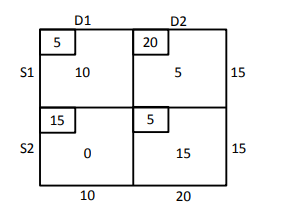
\includegraphics[width=0.75\columnwidth]{chapters/10/7/2/4/figs/fig.png}
 \end{center}
\caption{}
\label{fig:10/7/2/4Fig1}
\end{figure}
\fi

\item Find the position vector of the mid point of the vector joining the points $\vec{P}$(2, 3, 4)
and $\vec{Q}$(4, 1, –2).
\\
\solution
		\begin{enumerate}[label=\thesubsection.\arabic*,ref=\thesubsection.\theenumi]
\item Find the coordinates of the point which divides the join of $(-1,7) $ and $ (4,-3)$ in the ratio 2:3.
	\\
		\solution
	\input{chapters/10/7/2/1/section.tex}
\item Find the coordinates of the point $\vec{R}$ on the line segment joining the points $\vec{P}(-1,3)$ and $\vec{Q}(2,5)$ such that $PR=\frac{3}{5}PQ$.
\item Find the ratio in which the point $\vec{P}\brak{\frac{3}{4},\frac{5}{12}}$ divides the line segment joining the points $\vec{A}\brak{\frac{1}{2},\frac{3}{2}}$ and $ \vec{B}(2,-5)$.
\item Find the coordinates of the point which divides the line segment joining the points $(4,-3)$ and $(8,5)$ in the ratio $3:1$ internally.
\item Find the coordinates of the point $\vec{P}$ on $AD$ such that $AP : PD = 2 : 1$.
\item If the point $\vec{P} (2, 1)$ lies on the line segment joining points $\vec{A} (4, 2)$  and $ \vec{B} (8, 4)$,
then
\begin{enumerate}
	\item $AP =\frac{1}{3}{AB}$ 
\item ${AP}={PE}$
\item ${PB}=\frac{1}{3}{AB}$
\item${AP}=\frac{1}{2}{AB}$
 \end{enumerate}
\item Find the ratio in which the line segment joining the points $(-3,10)$  and  $(6,-8)$  is divided by $ (-1,6)$.
	\\
		\solution
	\input{chapters/10/7/2/4/section.tex}
\item Find the position vector of the mid point of the vector joining the points $\vec{P}$(2, 3, 4)
and $\vec{Q}$(4, 1, –2).
\\
\solution
		\input{chapters/12/10/2/16/section.tex}
\item Let $\vec{A}(4, 2), \vec{B}(6, 5)$  and $ \vec{C}(1, 4)$ be the vertices of $\triangle ABC$.
\begin{enumerate}
\item If $\vec{A}$ and  $\vec{B}$ are $(-2,-2)$ and  $(2,-4)$, respectively, find the coordinates of $\vec{P}$ such that $AP= \frac {3}{7}AB$  and $ \vec{P}$ lies on the line segment $AB$.
	\\
		\solution
	\input{chapters/10/7/2/8/section.tex}
\item Find the coordinates of the points which divide the line segment joining $A(-2,2)$  and  $\vec{B}(2,8)$ into four equal parts.
	\\
		\solution
	\input{chapters/10/7/2/9/section.tex}
\item In what ratio does the point $(-4,6)$ divide the line segment joining the points $\vec{A}(-6,0)$ and $\vec{B}(3,-8)$?
\item Given that $\vec{P}(3,2,-4), \vec{Q}(5,4,-6)$ and $\vec{R}(9,8,-10)$ are collinear. Find the ratio in which $\vec{Q}$ divides $PR$.
\item Points $\vec{A}(-6,10),\vec{B}(-4,6)$  and  $\vec{C}(3,-8)$ are collinear such that $AB=  \frac{2}{9}AC$.
\item The point which divides the line segment joining the points $\vec{P} (7, –6) $  and  $\vec{Q}(3, 4)$ in the 
ratio 1 : 2 internally lies in  which quadrant?
\item Find the coordinates of the points of trisection of the line segment joining $(4,-1)$  and  $(-2,3)$.
	\\
		\solution
	\input{chapters/10/7/2/2/section.tex}
\item Find the coordinates of the points which trisect the line segment joining the points $\vec{P}(4,2,-6)$ and $\vec{Q}(10,-16,6)$.
\item Find the coordinates of the points of trisection (i.e. points dividing to three equal parts) of the line segment joining the points $\vec{A}(2,-2)$ and $\vec{B}(-7,4)$.
\item Point $\vec{P}(5,-3)$ is one of the two points of trisection of line segment joining the points $\vec{A}(7,-2)$ and $\vec{B}(1,-5)$
\item Find the position vector of a point $\vec{R}$ which divides the line joining two points $\vec{P}$
and $\vec{Q}$ whose position vectors are $\hat{i}+2\hat{j}-\hat{k}$ and $-\hat{i}+\hat{j}+\hat{k}$ respectively, in the
ratio 2 : 1
\begin{enumerate}
    \item  internally
    \item  externally
\end{enumerate}
%\solution
%		\input{chapters/12/10/2/15/section.tex}
\item Find the coordinates of the point which divides the line segment joining the points which divides the line segment joining  the points $(-2,3,5)$ and $(1,-4,6)$ in the ratio 
\begin{enumerate}
\item $2:3$ internally,
\item $2:3$ externally
\end{enumerate}
\item Find the coordinates of the point which divides the line segment joining the points $(1,-2,3)$ and $(3,4,-5)$ in the ratio $2:3$
\begin{enumerate}
\item internally, and
\item externally
\end{enumerate}
\item Consider two points $\vec{P}$ and $\vec{Q}$ with position vectors $\overrightarrow{OP} = 3\overrightarrow{a}-2\overrightarrow{b}$ and $\overrightarrow{OQ}=\overrightarrow{a}+\overrightarrow{b}$. Find the position vector of a point $\vec{R}$ which divides the line joining $\vec{P}$ and $\vec{Q}$ in the ratio $2:1$, 
\begin{enumerate}
\item internally, and 
\item externally.
\end{enumerate}
\item The median from $\vec{A}$ meets $BC$ at $\vec{D}$. Find the coordinates of the point $\vec{D}$.
\item Find the coordinates of points $\vec{Q}$ and $\vec{R}$ on medians $BE$ and $CF$ respectively such that $BQ : QE = 2 : 1$  and  $CR : RF = 2 : 1$.
\item What do you observe?
\item If $\vec{A}, \vec{B}$ and $\vec{C}$  are the vertices of $\triangle ABC$, find the coordinates of the centroid of the triangle.
\end{enumerate}
\solution
	\input{chapters/10/7/4/7/section.tex}
\item If $\vec{P}(9a-2,-b)$ divides line segment joining $\vec{A}(3a+1,-3)$ and $\vec{B}(8a,5)$ in the ratio 3:1, find the values of $a$ and $b$.
\item Find the position vector of a point $\vec{R}$ which divides the line joining two points $\vec{P}$ and $\vec{Q}$ whose position vectors are $2\vec{a}+\vec{b}$ and $\vec{a}-3\vec{b}$ externally in the ratio $1:2$.
\item The position vector of the point which divides the join of points 2$\vec{a}$-3$\vec{b}$ $\text{and}$ $\vec{a}+\vec{b}$ in the ratio 3:1 is \rule{1cm}{0.1pt}.
\item If $\vec{a}$ and $\vec{b}$ are the postion vectors of $\vec{A}$ and $\vec{B}$, respectively, find the position vector of a point $\vec{C}$ in $BA$ produced such that $BC=1.5BA$.
\item Find the position vector of a point $\vec{R}$ which divides the line joining two points $\vec{P}$ and $\vec{Q}$ whose position vectors are $(2\vec{a}+\vec{b})$ and $(\vec{a}-3\vec{b})$
externally in the ratio 1 : 2. Also, show that $\vec{P}$ is the mid point of the line segment $RQ$.
\end{enumerate}

\item Let $\vec{A}(4, 2), \vec{B}(6, 5)$  and $ \vec{C}(1, 4)$ be the vertices of $\triangle ABC$.
\begin{enumerate}
\item If $\vec{A}$ and  $\vec{B}$ are $(-2,-2)$ and  $(2,-4)$, respectively, find the coordinates of $\vec{P}$ such that $AP= \frac {3}{7}AB$  and $ \vec{P}$ lies on the line segment $AB$.
	\\
		\solution
	\begin{enumerate}[label=\thesubsection.\arabic*,ref=\thesubsection.\theenumi]
\item Find the coordinates of the point which divides the join of $(-1,7) $ and $ (4,-3)$ in the ratio 2:3.
	\\
		\solution
	\input{chapters/10/7/2/1/section.tex}
\item Find the coordinates of the point $\vec{R}$ on the line segment joining the points $\vec{P}(-1,3)$ and $\vec{Q}(2,5)$ such that $PR=\frac{3}{5}PQ$.
\item Find the ratio in which the point $\vec{P}\brak{\frac{3}{4},\frac{5}{12}}$ divides the line segment joining the points $\vec{A}\brak{\frac{1}{2},\frac{3}{2}}$ and $ \vec{B}(2,-5)$.
\item Find the coordinates of the point which divides the line segment joining the points $(4,-3)$ and $(8,5)$ in the ratio $3:1$ internally.
\item Find the coordinates of the point $\vec{P}$ on $AD$ such that $AP : PD = 2 : 1$.
\item If the point $\vec{P} (2, 1)$ lies on the line segment joining points $\vec{A} (4, 2)$  and $ \vec{B} (8, 4)$,
then
\begin{enumerate}
	\item $AP =\frac{1}{3}{AB}$ 
\item ${AP}={PE}$
\item ${PB}=\frac{1}{3}{AB}$
\item${AP}=\frac{1}{2}{AB}$
 \end{enumerate}
\item Find the ratio in which the line segment joining the points $(-3,10)$  and  $(6,-8)$  is divided by $ (-1,6)$.
	\\
		\solution
	\input{chapters/10/7/2/4/section.tex}
\item Find the position vector of the mid point of the vector joining the points $\vec{P}$(2, 3, 4)
and $\vec{Q}$(4, 1, –2).
\\
\solution
		\input{chapters/12/10/2/16/section.tex}
\item Let $\vec{A}(4, 2), \vec{B}(6, 5)$  and $ \vec{C}(1, 4)$ be the vertices of $\triangle ABC$.
\begin{enumerate}
\item If $\vec{A}$ and  $\vec{B}$ are $(-2,-2)$ and  $(2,-4)$, respectively, find the coordinates of $\vec{P}$ such that $AP= \frac {3}{7}AB$  and $ \vec{P}$ lies on the line segment $AB$.
	\\
		\solution
	\input{chapters/10/7/2/8/section.tex}
\item Find the coordinates of the points which divide the line segment joining $A(-2,2)$  and  $\vec{B}(2,8)$ into four equal parts.
	\\
		\solution
	\input{chapters/10/7/2/9/section.tex}
\item In what ratio does the point $(-4,6)$ divide the line segment joining the points $\vec{A}(-6,0)$ and $\vec{B}(3,-8)$?
\item Given that $\vec{P}(3,2,-4), \vec{Q}(5,4,-6)$ and $\vec{R}(9,8,-10)$ are collinear. Find the ratio in which $\vec{Q}$ divides $PR$.
\item Points $\vec{A}(-6,10),\vec{B}(-4,6)$  and  $\vec{C}(3,-8)$ are collinear such that $AB=  \frac{2}{9}AC$.
\item The point which divides the line segment joining the points $\vec{P} (7, –6) $  and  $\vec{Q}(3, 4)$ in the 
ratio 1 : 2 internally lies in  which quadrant?
\item Find the coordinates of the points of trisection of the line segment joining $(4,-1)$  and  $(-2,3)$.
	\\
		\solution
	\input{chapters/10/7/2/2/section.tex}
\item Find the coordinates of the points which trisect the line segment joining the points $\vec{P}(4,2,-6)$ and $\vec{Q}(10,-16,6)$.
\item Find the coordinates of the points of trisection (i.e. points dividing to three equal parts) of the line segment joining the points $\vec{A}(2,-2)$ and $\vec{B}(-7,4)$.
\item Point $\vec{P}(5,-3)$ is one of the two points of trisection of line segment joining the points $\vec{A}(7,-2)$ and $\vec{B}(1,-5)$
\item Find the position vector of a point $\vec{R}$ which divides the line joining two points $\vec{P}$
and $\vec{Q}$ whose position vectors are $\hat{i}+2\hat{j}-\hat{k}$ and $-\hat{i}+\hat{j}+\hat{k}$ respectively, in the
ratio 2 : 1
\begin{enumerate}
    \item  internally
    \item  externally
\end{enumerate}
%\solution
%		\input{chapters/12/10/2/15/section.tex}
\item Find the coordinates of the point which divides the line segment joining the points which divides the line segment joining  the points $(-2,3,5)$ and $(1,-4,6)$ in the ratio 
\begin{enumerate}
\item $2:3$ internally,
\item $2:3$ externally
\end{enumerate}
\item Find the coordinates of the point which divides the line segment joining the points $(1,-2,3)$ and $(3,4,-5)$ in the ratio $2:3$
\begin{enumerate}
\item internally, and
\item externally
\end{enumerate}
\item Consider two points $\vec{P}$ and $\vec{Q}$ with position vectors $\overrightarrow{OP} = 3\overrightarrow{a}-2\overrightarrow{b}$ and $\overrightarrow{OQ}=\overrightarrow{a}+\overrightarrow{b}$. Find the position vector of a point $\vec{R}$ which divides the line joining $\vec{P}$ and $\vec{Q}$ in the ratio $2:1$, 
\begin{enumerate}
\item internally, and 
\item externally.
\end{enumerate}
\item The median from $\vec{A}$ meets $BC$ at $\vec{D}$. Find the coordinates of the point $\vec{D}$.
\item Find the coordinates of points $\vec{Q}$ and $\vec{R}$ on medians $BE$ and $CF$ respectively such that $BQ : QE = 2 : 1$  and  $CR : RF = 2 : 1$.
\item What do you observe?
\item If $\vec{A}, \vec{B}$ and $\vec{C}$  are the vertices of $\triangle ABC$, find the coordinates of the centroid of the triangle.
\end{enumerate}
\solution
	\input{chapters/10/7/4/7/section.tex}
\item If $\vec{P}(9a-2,-b)$ divides line segment joining $\vec{A}(3a+1,-3)$ and $\vec{B}(8a,5)$ in the ratio 3:1, find the values of $a$ and $b$.
\item Find the position vector of a point $\vec{R}$ which divides the line joining two points $\vec{P}$ and $\vec{Q}$ whose position vectors are $2\vec{a}+\vec{b}$ and $\vec{a}-3\vec{b}$ externally in the ratio $1:2$.
\item The position vector of the point which divides the join of points 2$\vec{a}$-3$\vec{b}$ $\text{and}$ $\vec{a}+\vec{b}$ in the ratio 3:1 is \rule{1cm}{0.1pt}.
\item If $\vec{a}$ and $\vec{b}$ are the postion vectors of $\vec{A}$ and $\vec{B}$, respectively, find the position vector of a point $\vec{C}$ in $BA$ produced such that $BC=1.5BA$.
\item Find the position vector of a point $\vec{R}$ which divides the line joining two points $\vec{P}$ and $\vec{Q}$ whose position vectors are $(2\vec{a}+\vec{b})$ and $(\vec{a}-3\vec{b})$
externally in the ratio 1 : 2. Also, show that $\vec{P}$ is the mid point of the line segment $RQ$.
\end{enumerate}

\item Find the coordinates of the points which divide the line segment joining $A(-2,2)$  and  $\vec{B}(2,8)$ into four equal parts.
	\\
		\solution
	\begin{enumerate}[label=\thesubsection.\arabic*,ref=\thesubsection.\theenumi]
\item Find the coordinates of the point which divides the join of $(-1,7) $ and $ (4,-3)$ in the ratio 2:3.
	\\
		\solution
	\input{chapters/10/7/2/1/section.tex}
\item Find the coordinates of the point $\vec{R}$ on the line segment joining the points $\vec{P}(-1,3)$ and $\vec{Q}(2,5)$ such that $PR=\frac{3}{5}PQ$.
\item Find the ratio in which the point $\vec{P}\brak{\frac{3}{4},\frac{5}{12}}$ divides the line segment joining the points $\vec{A}\brak{\frac{1}{2},\frac{3}{2}}$ and $ \vec{B}(2,-5)$.
\item Find the coordinates of the point which divides the line segment joining the points $(4,-3)$ and $(8,5)$ in the ratio $3:1$ internally.
\item Find the coordinates of the point $\vec{P}$ on $AD$ such that $AP : PD = 2 : 1$.
\item If the point $\vec{P} (2, 1)$ lies on the line segment joining points $\vec{A} (4, 2)$  and $ \vec{B} (8, 4)$,
then
\begin{enumerate}
	\item $AP =\frac{1}{3}{AB}$ 
\item ${AP}={PE}$
\item ${PB}=\frac{1}{3}{AB}$
\item${AP}=\frac{1}{2}{AB}$
 \end{enumerate}
\item Find the ratio in which the line segment joining the points $(-3,10)$  and  $(6,-8)$  is divided by $ (-1,6)$.
	\\
		\solution
	\input{chapters/10/7/2/4/section.tex}
\item Find the position vector of the mid point of the vector joining the points $\vec{P}$(2, 3, 4)
and $\vec{Q}$(4, 1, –2).
\\
\solution
		\input{chapters/12/10/2/16/section.tex}
\item Let $\vec{A}(4, 2), \vec{B}(6, 5)$  and $ \vec{C}(1, 4)$ be the vertices of $\triangle ABC$.
\begin{enumerate}
\item If $\vec{A}$ and  $\vec{B}$ are $(-2,-2)$ and  $(2,-4)$, respectively, find the coordinates of $\vec{P}$ such that $AP= \frac {3}{7}AB$  and $ \vec{P}$ lies on the line segment $AB$.
	\\
		\solution
	\input{chapters/10/7/2/8/section.tex}
\item Find the coordinates of the points which divide the line segment joining $A(-2,2)$  and  $\vec{B}(2,8)$ into four equal parts.
	\\
		\solution
	\input{chapters/10/7/2/9/section.tex}
\item In what ratio does the point $(-4,6)$ divide the line segment joining the points $\vec{A}(-6,0)$ and $\vec{B}(3,-8)$?
\item Given that $\vec{P}(3,2,-4), \vec{Q}(5,4,-6)$ and $\vec{R}(9,8,-10)$ are collinear. Find the ratio in which $\vec{Q}$ divides $PR$.
\item Points $\vec{A}(-6,10),\vec{B}(-4,6)$  and  $\vec{C}(3,-8)$ are collinear such that $AB=  \frac{2}{9}AC$.
\item The point which divides the line segment joining the points $\vec{P} (7, –6) $  and  $\vec{Q}(3, 4)$ in the 
ratio 1 : 2 internally lies in  which quadrant?
\item Find the coordinates of the points of trisection of the line segment joining $(4,-1)$  and  $(-2,3)$.
	\\
		\solution
	\input{chapters/10/7/2/2/section.tex}
\item Find the coordinates of the points which trisect the line segment joining the points $\vec{P}(4,2,-6)$ and $\vec{Q}(10,-16,6)$.
\item Find the coordinates of the points of trisection (i.e. points dividing to three equal parts) of the line segment joining the points $\vec{A}(2,-2)$ and $\vec{B}(-7,4)$.
\item Point $\vec{P}(5,-3)$ is one of the two points of trisection of line segment joining the points $\vec{A}(7,-2)$ and $\vec{B}(1,-5)$
\item Find the position vector of a point $\vec{R}$ which divides the line joining two points $\vec{P}$
and $\vec{Q}$ whose position vectors are $\hat{i}+2\hat{j}-\hat{k}$ and $-\hat{i}+\hat{j}+\hat{k}$ respectively, in the
ratio 2 : 1
\begin{enumerate}
    \item  internally
    \item  externally
\end{enumerate}
%\solution
%		\input{chapters/12/10/2/15/section.tex}
\item Find the coordinates of the point which divides the line segment joining the points which divides the line segment joining  the points $(-2,3,5)$ and $(1,-4,6)$ in the ratio 
\begin{enumerate}
\item $2:3$ internally,
\item $2:3$ externally
\end{enumerate}
\item Find the coordinates of the point which divides the line segment joining the points $(1,-2,3)$ and $(3,4,-5)$ in the ratio $2:3$
\begin{enumerate}
\item internally, and
\item externally
\end{enumerate}
\item Consider two points $\vec{P}$ and $\vec{Q}$ with position vectors $\overrightarrow{OP} = 3\overrightarrow{a}-2\overrightarrow{b}$ and $\overrightarrow{OQ}=\overrightarrow{a}+\overrightarrow{b}$. Find the position vector of a point $\vec{R}$ which divides the line joining $\vec{P}$ and $\vec{Q}$ in the ratio $2:1$, 
\begin{enumerate}
\item internally, and 
\item externally.
\end{enumerate}
\item The median from $\vec{A}$ meets $BC$ at $\vec{D}$. Find the coordinates of the point $\vec{D}$.
\item Find the coordinates of points $\vec{Q}$ and $\vec{R}$ on medians $BE$ and $CF$ respectively such that $BQ : QE = 2 : 1$  and  $CR : RF = 2 : 1$.
\item What do you observe?
\item If $\vec{A}, \vec{B}$ and $\vec{C}$  are the vertices of $\triangle ABC$, find the coordinates of the centroid of the triangle.
\end{enumerate}
\solution
	\input{chapters/10/7/4/7/section.tex}
\item If $\vec{P}(9a-2,-b)$ divides line segment joining $\vec{A}(3a+1,-3)$ and $\vec{B}(8a,5)$ in the ratio 3:1, find the values of $a$ and $b$.
\item Find the position vector of a point $\vec{R}$ which divides the line joining two points $\vec{P}$ and $\vec{Q}$ whose position vectors are $2\vec{a}+\vec{b}$ and $\vec{a}-3\vec{b}$ externally in the ratio $1:2$.
\item The position vector of the point which divides the join of points 2$\vec{a}$-3$\vec{b}$ $\text{and}$ $\vec{a}+\vec{b}$ in the ratio 3:1 is \rule{1cm}{0.1pt}.
\item If $\vec{a}$ and $\vec{b}$ are the postion vectors of $\vec{A}$ and $\vec{B}$, respectively, find the position vector of a point $\vec{C}$ in $BA$ produced such that $BC=1.5BA$.
\item Find the position vector of a point $\vec{R}$ which divides the line joining two points $\vec{P}$ and $\vec{Q}$ whose position vectors are $(2\vec{a}+\vec{b})$ and $(\vec{a}-3\vec{b})$
externally in the ratio 1 : 2. Also, show that $\vec{P}$ is the mid point of the line segment $RQ$.
\end{enumerate}

\item In what ratio does the point $(-4,6)$ divide the line segment joining the points $\vec{A}(-6,0)$ and $\vec{B}(3,-8)$?
\item Given that $\vec{P}(3,2,-4), \vec{Q}(5,4,-6)$ and $\vec{R}(9,8,-10)$ are collinear. Find the ratio in which $\vec{Q}$ divides $PR$.
\item Points $\vec{A}(-6,10),\vec{B}(-4,6)$  and  $\vec{C}(3,-8)$ are collinear such that $AB=  \frac{2}{9}AC$.
\item The point which divides the line segment joining the points $\vec{P} (7, –6) $  and  $\vec{Q}(3, 4)$ in the 
ratio 1 : 2 internally lies in  which quadrant?
\item Find the coordinates of the points of trisection of the line segment joining $(4,-1)$  and  $(-2,3)$.
	\\
		\solution
	Using section formula,
\begin{align}
\vec{R}=\frac{1}{1+\frac{1}{2}}\brak{\myvec{4\\-1}+\frac{1}{2}\myvec{-2\\3}}
=\myvec{2\\ \frac{1}{3}}\\
\vec{S}=\frac{1}{1+\frac{2}{1}}\brak{\myvec{4\\-1}+\frac{2}{1}\myvec{-2\\3}}
=\myvec{0\\ \frac{5}{3}}
\end{align}
which are the desired points of trisection.
\iffalse
See
		\figref{fig:chapters/10/7/2/2/Figure}
\begin{figure}[H]
\centering
\includegraphics[width=0.75\columnwidth]{chapters/10/7/2/2/figs/dj.pdf}
\caption{}
		\label{fig:chapters/10/7/2/2/Figure}
\end{figure}
\fi

\item Find the coordinates of the points which trisect the line segment joining the points $\vec{P}(4,2,-6)$ and $\vec{Q}(10,-16,6)$.
\item Find the coordinates of the points of trisection (i.e. points dividing to three equal parts) of the line segment joining the points $\vec{A}(2,-2)$ and $\vec{B}(-7,4)$.
\item Point $\vec{P}(5,-3)$ is one of the two points of trisection of line segment joining the points $\vec{A}(7,-2)$ and $\vec{B}(1,-5)$
\item Find the position vector of a point $\vec{R}$ which divides the line joining two points $\vec{P}$
and $\vec{Q}$ whose position vectors are $\hat{i}+2\hat{j}-\hat{k}$ and $-\hat{i}+\hat{j}+\hat{k}$ respectively, in the
ratio 2 : 1
\begin{enumerate}
    \item  internally
    \item  externally
\end{enumerate}
%\solution
%		\begin{enumerate}[label=\thesubsection.\arabic*,ref=\thesubsection.\theenumi]
\item Find the coordinates of the point which divides the join of $(-1,7) $ and $ (4,-3)$ in the ratio 2:3.
	\\
		\solution
	\input{chapters/10/7/2/1/section.tex}
\item Find the coordinates of the point $\vec{R}$ on the line segment joining the points $\vec{P}(-1,3)$ and $\vec{Q}(2,5)$ such that $PR=\frac{3}{5}PQ$.
\item Find the ratio in which the point $\vec{P}\brak{\frac{3}{4},\frac{5}{12}}$ divides the line segment joining the points $\vec{A}\brak{\frac{1}{2},\frac{3}{2}}$ and $ \vec{B}(2,-5)$.
\item Find the coordinates of the point which divides the line segment joining the points $(4,-3)$ and $(8,5)$ in the ratio $3:1$ internally.
\item Find the coordinates of the point $\vec{P}$ on $AD$ such that $AP : PD = 2 : 1$.
\item If the point $\vec{P} (2, 1)$ lies on the line segment joining points $\vec{A} (4, 2)$  and $ \vec{B} (8, 4)$,
then
\begin{enumerate}
	\item $AP =\frac{1}{3}{AB}$ 
\item ${AP}={PE}$
\item ${PB}=\frac{1}{3}{AB}$
\item${AP}=\frac{1}{2}{AB}$
 \end{enumerate}
\item Find the ratio in which the line segment joining the points $(-3,10)$  and  $(6,-8)$  is divided by $ (-1,6)$.
	\\
		\solution
	\input{chapters/10/7/2/4/section.tex}
\item Find the position vector of the mid point of the vector joining the points $\vec{P}$(2, 3, 4)
and $\vec{Q}$(4, 1, –2).
\\
\solution
		\input{chapters/12/10/2/16/section.tex}
\item Let $\vec{A}(4, 2), \vec{B}(6, 5)$  and $ \vec{C}(1, 4)$ be the vertices of $\triangle ABC$.
\begin{enumerate}
\item If $\vec{A}$ and  $\vec{B}$ are $(-2,-2)$ and  $(2,-4)$, respectively, find the coordinates of $\vec{P}$ such that $AP= \frac {3}{7}AB$  and $ \vec{P}$ lies on the line segment $AB$.
	\\
		\solution
	\input{chapters/10/7/2/8/section.tex}
\item Find the coordinates of the points which divide the line segment joining $A(-2,2)$  and  $\vec{B}(2,8)$ into four equal parts.
	\\
		\solution
	\input{chapters/10/7/2/9/section.tex}
\item In what ratio does the point $(-4,6)$ divide the line segment joining the points $\vec{A}(-6,0)$ and $\vec{B}(3,-8)$?
\item Given that $\vec{P}(3,2,-4), \vec{Q}(5,4,-6)$ and $\vec{R}(9,8,-10)$ are collinear. Find the ratio in which $\vec{Q}$ divides $PR$.
\item Points $\vec{A}(-6,10),\vec{B}(-4,6)$  and  $\vec{C}(3,-8)$ are collinear such that $AB=  \frac{2}{9}AC$.
\item The point which divides the line segment joining the points $\vec{P} (7, –6) $  and  $\vec{Q}(3, 4)$ in the 
ratio 1 : 2 internally lies in  which quadrant?
\item Find the coordinates of the points of trisection of the line segment joining $(4,-1)$  and  $(-2,3)$.
	\\
		\solution
	\input{chapters/10/7/2/2/section.tex}
\item Find the coordinates of the points which trisect the line segment joining the points $\vec{P}(4,2,-6)$ and $\vec{Q}(10,-16,6)$.
\item Find the coordinates of the points of trisection (i.e. points dividing to three equal parts) of the line segment joining the points $\vec{A}(2,-2)$ and $\vec{B}(-7,4)$.
\item Point $\vec{P}(5,-3)$ is one of the two points of trisection of line segment joining the points $\vec{A}(7,-2)$ and $\vec{B}(1,-5)$
\item Find the position vector of a point $\vec{R}$ which divides the line joining two points $\vec{P}$
and $\vec{Q}$ whose position vectors are $\hat{i}+2\hat{j}-\hat{k}$ and $-\hat{i}+\hat{j}+\hat{k}$ respectively, in the
ratio 2 : 1
\begin{enumerate}
    \item  internally
    \item  externally
\end{enumerate}
%\solution
%		\input{chapters/12/10/2/15/section.tex}
\item Find the coordinates of the point which divides the line segment joining the points which divides the line segment joining  the points $(-2,3,5)$ and $(1,-4,6)$ in the ratio 
\begin{enumerate}
\item $2:3$ internally,
\item $2:3$ externally
\end{enumerate}
\item Find the coordinates of the point which divides the line segment joining the points $(1,-2,3)$ and $(3,4,-5)$ in the ratio $2:3$
\begin{enumerate}
\item internally, and
\item externally
\end{enumerate}
\item Consider two points $\vec{P}$ and $\vec{Q}$ with position vectors $\overrightarrow{OP} = 3\overrightarrow{a}-2\overrightarrow{b}$ and $\overrightarrow{OQ}=\overrightarrow{a}+\overrightarrow{b}$. Find the position vector of a point $\vec{R}$ which divides the line joining $\vec{P}$ and $\vec{Q}$ in the ratio $2:1$, 
\begin{enumerate}
\item internally, and 
\item externally.
\end{enumerate}
\item The median from $\vec{A}$ meets $BC$ at $\vec{D}$. Find the coordinates of the point $\vec{D}$.
\item Find the coordinates of points $\vec{Q}$ and $\vec{R}$ on medians $BE$ and $CF$ respectively such that $BQ : QE = 2 : 1$  and  $CR : RF = 2 : 1$.
\item What do you observe?
\item If $\vec{A}, \vec{B}$ and $\vec{C}$  are the vertices of $\triangle ABC$, find the coordinates of the centroid of the triangle.
\end{enumerate}
\solution
	\input{chapters/10/7/4/7/section.tex}
\item If $\vec{P}(9a-2,-b)$ divides line segment joining $\vec{A}(3a+1,-3)$ and $\vec{B}(8a,5)$ in the ratio 3:1, find the values of $a$ and $b$.
\item Find the position vector of a point $\vec{R}$ which divides the line joining two points $\vec{P}$ and $\vec{Q}$ whose position vectors are $2\vec{a}+\vec{b}$ and $\vec{a}-3\vec{b}$ externally in the ratio $1:2$.
\item The position vector of the point which divides the join of points 2$\vec{a}$-3$\vec{b}$ $\text{and}$ $\vec{a}+\vec{b}$ in the ratio 3:1 is \rule{1cm}{0.1pt}.
\item If $\vec{a}$ and $\vec{b}$ are the postion vectors of $\vec{A}$ and $\vec{B}$, respectively, find the position vector of a point $\vec{C}$ in $BA$ produced such that $BC=1.5BA$.
\item Find the position vector of a point $\vec{R}$ which divides the line joining two points $\vec{P}$ and $\vec{Q}$ whose position vectors are $(2\vec{a}+\vec{b})$ and $(\vec{a}-3\vec{b})$
externally in the ratio 1 : 2. Also, show that $\vec{P}$ is the mid point of the line segment $RQ$.
\end{enumerate}

\item Find the coordinates of the point which divides the line segment joining the points which divides the line segment joining  the points $(-2,3,5)$ and $(1,-4,6)$ in the ratio 
\begin{enumerate}
\item $2:3$ internally,
\item $2:3$ externally
\end{enumerate}
\item Find the coordinates of the point which divides the line segment joining the points $(1,-2,3)$ and $(3,4,-5)$ in the ratio $2:3$
\begin{enumerate}
\item internally, and
\item externally
\end{enumerate}
\item Consider two points $\vec{P}$ and $\vec{Q}$ with position vectors $\overrightarrow{OP} = 3\overrightarrow{a}-2\overrightarrow{b}$ and $\overrightarrow{OQ}=\overrightarrow{a}+\overrightarrow{b}$. Find the position vector of a point $\vec{R}$ which divides the line joining $\vec{P}$ and $\vec{Q}$ in the ratio $2:1$, 
\begin{enumerate}
\item internally, and 
\item externally.
\end{enumerate}
\item The median from $\vec{A}$ meets $BC$ at $\vec{D}$. Find the coordinates of the point $\vec{D}$.
\item Find the coordinates of points $\vec{Q}$ and $\vec{R}$ on medians $BE$ and $CF$ respectively such that $BQ : QE = 2 : 1$  and  $CR : RF = 2 : 1$.
\item What do you observe?
\item If $\vec{A}, \vec{B}$ and $\vec{C}$  are the vertices of $\triangle ABC$, find the coordinates of the centroid of the triangle.
\end{enumerate}
\solution
	\begin{enumerate}[label=\thesubsection.\arabic*,ref=\thesubsection.\theenumi]
\item Find the coordinates of the point which divides the join of $(-1,7) $ and $ (4,-3)$ in the ratio 2:3.
	\\
		\solution
	\input{chapters/10/7/2/1/section.tex}
\item Find the coordinates of the point $\vec{R}$ on the line segment joining the points $\vec{P}(-1,3)$ and $\vec{Q}(2,5)$ such that $PR=\frac{3}{5}PQ$.
\item Find the ratio in which the point $\vec{P}\brak{\frac{3}{4},\frac{5}{12}}$ divides the line segment joining the points $\vec{A}\brak{\frac{1}{2},\frac{3}{2}}$ and $ \vec{B}(2,-5)$.
\item Find the coordinates of the point which divides the line segment joining the points $(4,-3)$ and $(8,5)$ in the ratio $3:1$ internally.
\item Find the coordinates of the point $\vec{P}$ on $AD$ such that $AP : PD = 2 : 1$.
\item If the point $\vec{P} (2, 1)$ lies on the line segment joining points $\vec{A} (4, 2)$  and $ \vec{B} (8, 4)$,
then
\begin{enumerate}
	\item $AP =\frac{1}{3}{AB}$ 
\item ${AP}={PE}$
\item ${PB}=\frac{1}{3}{AB}$
\item${AP}=\frac{1}{2}{AB}$
 \end{enumerate}
\item Find the ratio in which the line segment joining the points $(-3,10)$  and  $(6,-8)$  is divided by $ (-1,6)$.
	\\
		\solution
	\input{chapters/10/7/2/4/section.tex}
\item Find the position vector of the mid point of the vector joining the points $\vec{P}$(2, 3, 4)
and $\vec{Q}$(4, 1, –2).
\\
\solution
		\input{chapters/12/10/2/16/section.tex}
\item Let $\vec{A}(4, 2), \vec{B}(6, 5)$  and $ \vec{C}(1, 4)$ be the vertices of $\triangle ABC$.
\begin{enumerate}
\item If $\vec{A}$ and  $\vec{B}$ are $(-2,-2)$ and  $(2,-4)$, respectively, find the coordinates of $\vec{P}$ such that $AP= \frac {3}{7}AB$  and $ \vec{P}$ lies on the line segment $AB$.
	\\
		\solution
	\input{chapters/10/7/2/8/section.tex}
\item Find the coordinates of the points which divide the line segment joining $A(-2,2)$  and  $\vec{B}(2,8)$ into four equal parts.
	\\
		\solution
	\input{chapters/10/7/2/9/section.tex}
\item In what ratio does the point $(-4,6)$ divide the line segment joining the points $\vec{A}(-6,0)$ and $\vec{B}(3,-8)$?
\item Given that $\vec{P}(3,2,-4), \vec{Q}(5,4,-6)$ and $\vec{R}(9,8,-10)$ are collinear. Find the ratio in which $\vec{Q}$ divides $PR$.
\item Points $\vec{A}(-6,10),\vec{B}(-4,6)$  and  $\vec{C}(3,-8)$ are collinear such that $AB=  \frac{2}{9}AC$.
\item The point which divides the line segment joining the points $\vec{P} (7, –6) $  and  $\vec{Q}(3, 4)$ in the 
ratio 1 : 2 internally lies in  which quadrant?
\item Find the coordinates of the points of trisection of the line segment joining $(4,-1)$  and  $(-2,3)$.
	\\
		\solution
	\input{chapters/10/7/2/2/section.tex}
\item Find the coordinates of the points which trisect the line segment joining the points $\vec{P}(4,2,-6)$ and $\vec{Q}(10,-16,6)$.
\item Find the coordinates of the points of trisection (i.e. points dividing to three equal parts) of the line segment joining the points $\vec{A}(2,-2)$ and $\vec{B}(-7,4)$.
\item Point $\vec{P}(5,-3)$ is one of the two points of trisection of line segment joining the points $\vec{A}(7,-2)$ and $\vec{B}(1,-5)$
\item Find the position vector of a point $\vec{R}$ which divides the line joining two points $\vec{P}$
and $\vec{Q}$ whose position vectors are $\hat{i}+2\hat{j}-\hat{k}$ and $-\hat{i}+\hat{j}+\hat{k}$ respectively, in the
ratio 2 : 1
\begin{enumerate}
    \item  internally
    \item  externally
\end{enumerate}
%\solution
%		\input{chapters/12/10/2/15/section.tex}
\item Find the coordinates of the point which divides the line segment joining the points which divides the line segment joining  the points $(-2,3,5)$ and $(1,-4,6)$ in the ratio 
\begin{enumerate}
\item $2:3$ internally,
\item $2:3$ externally
\end{enumerate}
\item Find the coordinates of the point which divides the line segment joining the points $(1,-2,3)$ and $(3,4,-5)$ in the ratio $2:3$
\begin{enumerate}
\item internally, and
\item externally
\end{enumerate}
\item Consider two points $\vec{P}$ and $\vec{Q}$ with position vectors $\overrightarrow{OP} = 3\overrightarrow{a}-2\overrightarrow{b}$ and $\overrightarrow{OQ}=\overrightarrow{a}+\overrightarrow{b}$. Find the position vector of a point $\vec{R}$ which divides the line joining $\vec{P}$ and $\vec{Q}$ in the ratio $2:1$, 
\begin{enumerate}
\item internally, and 
\item externally.
\end{enumerate}
\item The median from $\vec{A}$ meets $BC$ at $\vec{D}$. Find the coordinates of the point $\vec{D}$.
\item Find the coordinates of points $\vec{Q}$ and $\vec{R}$ on medians $BE$ and $CF$ respectively such that $BQ : QE = 2 : 1$  and  $CR : RF = 2 : 1$.
\item What do you observe?
\item If $\vec{A}, \vec{B}$ and $\vec{C}$  are the vertices of $\triangle ABC$, find the coordinates of the centroid of the triangle.
\end{enumerate}
\solution
	\input{chapters/10/7/4/7/section.tex}
\item If $\vec{P}(9a-2,-b)$ divides line segment joining $\vec{A}(3a+1,-3)$ and $\vec{B}(8a,5)$ in the ratio 3:1, find the values of $a$ and $b$.
\item Find the position vector of a point $\vec{R}$ which divides the line joining two points $\vec{P}$ and $\vec{Q}$ whose position vectors are $2\vec{a}+\vec{b}$ and $\vec{a}-3\vec{b}$ externally in the ratio $1:2$.
\item The position vector of the point which divides the join of points 2$\vec{a}$-3$\vec{b}$ $\text{and}$ $\vec{a}+\vec{b}$ in the ratio 3:1 is \rule{1cm}{0.1pt}.
\item If $\vec{a}$ and $\vec{b}$ are the postion vectors of $\vec{A}$ and $\vec{B}$, respectively, find the position vector of a point $\vec{C}$ in $BA$ produced such that $BC=1.5BA$.
\item Find the position vector of a point $\vec{R}$ which divides the line joining two points $\vec{P}$ and $\vec{Q}$ whose position vectors are $(2\vec{a}+\vec{b})$ and $(\vec{a}-3\vec{b})$
externally in the ratio 1 : 2. Also, show that $\vec{P}$ is the mid point of the line segment $RQ$.
\end{enumerate}

\item If $\vec{P}(9a-2,-b)$ divides line segment joining $\vec{A}(3a+1,-3)$ and $\vec{B}(8a,5)$ in the ratio 3:1, find the values of $a$ and $b$.
\item Find the position vector of a point $\vec{R}$ which divides the line joining two points $\vec{P}$ and $\vec{Q}$ whose position vectors are $2\vec{a}+\vec{b}$ and $\vec{a}-3\vec{b}$ externally in the ratio $1:2$.
\item The position vector of the point which divides the join of points 2$\vec{a}$-3$\vec{b}$ $\text{and}$ $\vec{a}+\vec{b}$ in the ratio 3:1 is \rule{1cm}{0.1pt}.
\item If $\vec{a}$ and $\vec{b}$ are the postion vectors of $\vec{A}$ and $\vec{B}$, respectively, find the position vector of a point $\vec{C}$ in $BA$ produced such that $BC=1.5BA$.
\item Find the position vector of a point $\vec{R}$ which divides the line joining two points $\vec{P}$ and $\vec{Q}$ whose position vectors are $(2\vec{a}+\vec{b})$ and $(\vec{a}-3\vec{b})$
externally in the ratio 1 : 2. Also, show that $\vec{P}$ is the mid point of the line segment $RQ$.
\end{enumerate}

\item Let $\vec{A}(4, 2), \vec{B}(6, 5)$  and $ \vec{C}(1, 4)$ be the vertices of $\triangle ABC$.
\begin{enumerate}
\item If $\vec{A}$ and  $\vec{B}$ are $(-2,-2)$ and  $(2,-4)$, respectively, find the coordinates of $\vec{P}$ such that $AP= \frac {3}{7}AB$  and $ \vec{P}$ lies on the line segment $AB$.
	\\
		\solution
	\begin{enumerate}[label=\thesubsection.\arabic*,ref=\thesubsection.\theenumi]
\item Find the coordinates of the point which divides the join of $(-1,7) $ and $ (4,-3)$ in the ratio 2:3.
	\\
		\solution
	\begin{enumerate}[label=\thesubsection.\arabic*,ref=\thesubsection.\theenumi]
\item Find the coordinates of the point which divides the join of $(-1,7) $ and $ (4,-3)$ in the ratio 2:3.
	\\
		\solution
	\input{chapters/10/7/2/1/section.tex}
\item Find the coordinates of the point $\vec{R}$ on the line segment joining the points $\vec{P}(-1,3)$ and $\vec{Q}(2,5)$ such that $PR=\frac{3}{5}PQ$.
\item Find the ratio in which the point $\vec{P}\brak{\frac{3}{4},\frac{5}{12}}$ divides the line segment joining the points $\vec{A}\brak{\frac{1}{2},\frac{3}{2}}$ and $ \vec{B}(2,-5)$.
\item Find the coordinates of the point which divides the line segment joining the points $(4,-3)$ and $(8,5)$ in the ratio $3:1$ internally.
\item Find the coordinates of the point $\vec{P}$ on $AD$ such that $AP : PD = 2 : 1$.
\item If the point $\vec{P} (2, 1)$ lies on the line segment joining points $\vec{A} (4, 2)$  and $ \vec{B} (8, 4)$,
then
\begin{enumerate}
	\item $AP =\frac{1}{3}{AB}$ 
\item ${AP}={PE}$
\item ${PB}=\frac{1}{3}{AB}$
\item${AP}=\frac{1}{2}{AB}$
 \end{enumerate}
\item Find the ratio in which the line segment joining the points $(-3,10)$  and  $(6,-8)$  is divided by $ (-1,6)$.
	\\
		\solution
	\input{chapters/10/7/2/4/section.tex}
\item Find the position vector of the mid point of the vector joining the points $\vec{P}$(2, 3, 4)
and $\vec{Q}$(4, 1, –2).
\\
\solution
		\input{chapters/12/10/2/16/section.tex}
\item Let $\vec{A}(4, 2), \vec{B}(6, 5)$  and $ \vec{C}(1, 4)$ be the vertices of $\triangle ABC$.
\begin{enumerate}
\item If $\vec{A}$ and  $\vec{B}$ are $(-2,-2)$ and  $(2,-4)$, respectively, find the coordinates of $\vec{P}$ such that $AP= \frac {3}{7}AB$  and $ \vec{P}$ lies on the line segment $AB$.
	\\
		\solution
	\input{chapters/10/7/2/8/section.tex}
\item Find the coordinates of the points which divide the line segment joining $A(-2,2)$  and  $\vec{B}(2,8)$ into four equal parts.
	\\
		\solution
	\input{chapters/10/7/2/9/section.tex}
\item In what ratio does the point $(-4,6)$ divide the line segment joining the points $\vec{A}(-6,0)$ and $\vec{B}(3,-8)$?
\item Given that $\vec{P}(3,2,-4), \vec{Q}(5,4,-6)$ and $\vec{R}(9,8,-10)$ are collinear. Find the ratio in which $\vec{Q}$ divides $PR$.
\item Points $\vec{A}(-6,10),\vec{B}(-4,6)$  and  $\vec{C}(3,-8)$ are collinear such that $AB=  \frac{2}{9}AC$.
\item The point which divides the line segment joining the points $\vec{P} (7, –6) $  and  $\vec{Q}(3, 4)$ in the 
ratio 1 : 2 internally lies in  which quadrant?
\item Find the coordinates of the points of trisection of the line segment joining $(4,-1)$  and  $(-2,3)$.
	\\
		\solution
	\input{chapters/10/7/2/2/section.tex}
\item Find the coordinates of the points which trisect the line segment joining the points $\vec{P}(4,2,-6)$ and $\vec{Q}(10,-16,6)$.
\item Find the coordinates of the points of trisection (i.e. points dividing to three equal parts) of the line segment joining the points $\vec{A}(2,-2)$ and $\vec{B}(-7,4)$.
\item Point $\vec{P}(5,-3)$ is one of the two points of trisection of line segment joining the points $\vec{A}(7,-2)$ and $\vec{B}(1,-5)$
\item Find the position vector of a point $\vec{R}$ which divides the line joining two points $\vec{P}$
and $\vec{Q}$ whose position vectors are $\hat{i}+2\hat{j}-\hat{k}$ and $-\hat{i}+\hat{j}+\hat{k}$ respectively, in the
ratio 2 : 1
\begin{enumerate}
    \item  internally
    \item  externally
\end{enumerate}
%\solution
%		\input{chapters/12/10/2/15/section.tex}
\item Find the coordinates of the point which divides the line segment joining the points which divides the line segment joining  the points $(-2,3,5)$ and $(1,-4,6)$ in the ratio 
\begin{enumerate}
\item $2:3$ internally,
\item $2:3$ externally
\end{enumerate}
\item Find the coordinates of the point which divides the line segment joining the points $(1,-2,3)$ and $(3,4,-5)$ in the ratio $2:3$
\begin{enumerate}
\item internally, and
\item externally
\end{enumerate}
\item Consider two points $\vec{P}$ and $\vec{Q}$ with position vectors $\overrightarrow{OP} = 3\overrightarrow{a}-2\overrightarrow{b}$ and $\overrightarrow{OQ}=\overrightarrow{a}+\overrightarrow{b}$. Find the position vector of a point $\vec{R}$ which divides the line joining $\vec{P}$ and $\vec{Q}$ in the ratio $2:1$, 
\begin{enumerate}
\item internally, and 
\item externally.
\end{enumerate}
\item The median from $\vec{A}$ meets $BC$ at $\vec{D}$. Find the coordinates of the point $\vec{D}$.
\item Find the coordinates of points $\vec{Q}$ and $\vec{R}$ on medians $BE$ and $CF$ respectively such that $BQ : QE = 2 : 1$  and  $CR : RF = 2 : 1$.
\item What do you observe?
\item If $\vec{A}, \vec{B}$ and $\vec{C}$  are the vertices of $\triangle ABC$, find the coordinates of the centroid of the triangle.
\end{enumerate}
\solution
	\input{chapters/10/7/4/7/section.tex}
\item If $\vec{P}(9a-2,-b)$ divides line segment joining $\vec{A}(3a+1,-3)$ and $\vec{B}(8a,5)$ in the ratio 3:1, find the values of $a$ and $b$.
\item Find the position vector of a point $\vec{R}$ which divides the line joining two points $\vec{P}$ and $\vec{Q}$ whose position vectors are $2\vec{a}+\vec{b}$ and $\vec{a}-3\vec{b}$ externally in the ratio $1:2$.
\item The position vector of the point which divides the join of points 2$\vec{a}$-3$\vec{b}$ $\text{and}$ $\vec{a}+\vec{b}$ in the ratio 3:1 is \rule{1cm}{0.1pt}.
\item If $\vec{a}$ and $\vec{b}$ are the postion vectors of $\vec{A}$ and $\vec{B}$, respectively, find the position vector of a point $\vec{C}$ in $BA$ produced such that $BC=1.5BA$.
\item Find the position vector of a point $\vec{R}$ which divides the line joining two points $\vec{P}$ and $\vec{Q}$ whose position vectors are $(2\vec{a}+\vec{b})$ and $(\vec{a}-3\vec{b})$
externally in the ratio 1 : 2. Also, show that $\vec{P}$ is the mid point of the line segment $RQ$.
\end{enumerate}

\item Find the coordinates of the point $\vec{R}$ on the line segment joining the points $\vec{P}(-1,3)$ and $\vec{Q}(2,5)$ such that $PR=\frac{3}{5}PQ$.
\item Find the ratio in which the point $\vec{P}\brak{\frac{3}{4},\frac{5}{12}}$ divides the line segment joining the points $\vec{A}\brak{\frac{1}{2},\frac{3}{2}}$ and $ \vec{B}(2,-5)$.
\item Find the coordinates of the point which divides the line segment joining the points $(4,-3)$ and $(8,5)$ in the ratio $3:1$ internally.
\item Find the coordinates of the point $\vec{P}$ on $AD$ such that $AP : PD = 2 : 1$.
\item If the point $\vec{P} (2, 1)$ lies on the line segment joining points $\vec{A} (4, 2)$  and $ \vec{B} (8, 4)$,
then
\begin{enumerate}
	\item $AP =\frac{1}{3}{AB}$ 
\item ${AP}={PE}$
\item ${PB}=\frac{1}{3}{AB}$
\item${AP}=\frac{1}{2}{AB}$
 \end{enumerate}
\item Find the ratio in which the line segment joining the points $(-3,10)$  and  $(6,-8)$  is divided by $ (-1,6)$.
	\\
		\solution
	\iffalse
Using section formula,
\begin{align}
         \myvec{-1\\6} &=\frac{{\myvec{-3\\10}+k\myvec{6\\-8}}}{1+k}\\
	 \implies 7k\myvec{1 \\ -2} &= 2\myvec{1 \\ -2}
	 \\
	 \text{or, } k &= \frac{2}{7}.
\end{align}
\fi
In 
			\eqref{eq:section_formula-k}, substituting
			\begin{align}
				\vec{B} &= \myvec{-3\\10}, \vec{C} = \myvec{6\\-8}, \vec{D} = \myvec{-1\\6},
				\\
				k &= \frac{\myvec{-2 & 4}\myvec{-7 \\ 14}}{\norm{\myvec{-7 \\ 14}}^2} = \frac{2}{7}
			\end{align}
\iffalse
See \figref{fig:10/7/2/4Fig1}.
\begin{figure}[H]
 \begin{center}
  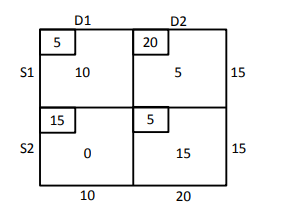
\includegraphics[width=0.75\columnwidth]{chapters/10/7/2/4/figs/fig.png}
 \end{center}
\caption{}
\label{fig:10/7/2/4Fig1}
\end{figure}
\fi

\item Find the position vector of the mid point of the vector joining the points $\vec{P}$(2, 3, 4)
and $\vec{Q}$(4, 1, –2).
\\
\solution
		\begin{enumerate}[label=\thesubsection.\arabic*,ref=\thesubsection.\theenumi]
\item Find the coordinates of the point which divides the join of $(-1,7) $ and $ (4,-3)$ in the ratio 2:3.
	\\
		\solution
	\input{chapters/10/7/2/1/section.tex}
\item Find the coordinates of the point $\vec{R}$ on the line segment joining the points $\vec{P}(-1,3)$ and $\vec{Q}(2,5)$ such that $PR=\frac{3}{5}PQ$.
\item Find the ratio in which the point $\vec{P}\brak{\frac{3}{4},\frac{5}{12}}$ divides the line segment joining the points $\vec{A}\brak{\frac{1}{2},\frac{3}{2}}$ and $ \vec{B}(2,-5)$.
\item Find the coordinates of the point which divides the line segment joining the points $(4,-3)$ and $(8,5)$ in the ratio $3:1$ internally.
\item Find the coordinates of the point $\vec{P}$ on $AD$ such that $AP : PD = 2 : 1$.
\item If the point $\vec{P} (2, 1)$ lies on the line segment joining points $\vec{A} (4, 2)$  and $ \vec{B} (8, 4)$,
then
\begin{enumerate}
	\item $AP =\frac{1}{3}{AB}$ 
\item ${AP}={PE}$
\item ${PB}=\frac{1}{3}{AB}$
\item${AP}=\frac{1}{2}{AB}$
 \end{enumerate}
\item Find the ratio in which the line segment joining the points $(-3,10)$  and  $(6,-8)$  is divided by $ (-1,6)$.
	\\
		\solution
	\input{chapters/10/7/2/4/section.tex}
\item Find the position vector of the mid point of the vector joining the points $\vec{P}$(2, 3, 4)
and $\vec{Q}$(4, 1, –2).
\\
\solution
		\input{chapters/12/10/2/16/section.tex}
\item Let $\vec{A}(4, 2), \vec{B}(6, 5)$  and $ \vec{C}(1, 4)$ be the vertices of $\triangle ABC$.
\begin{enumerate}
\item If $\vec{A}$ and  $\vec{B}$ are $(-2,-2)$ and  $(2,-4)$, respectively, find the coordinates of $\vec{P}$ such that $AP= \frac {3}{7}AB$  and $ \vec{P}$ lies on the line segment $AB$.
	\\
		\solution
	\input{chapters/10/7/2/8/section.tex}
\item Find the coordinates of the points which divide the line segment joining $A(-2,2)$  and  $\vec{B}(2,8)$ into four equal parts.
	\\
		\solution
	\input{chapters/10/7/2/9/section.tex}
\item In what ratio does the point $(-4,6)$ divide the line segment joining the points $\vec{A}(-6,0)$ and $\vec{B}(3,-8)$?
\item Given that $\vec{P}(3,2,-4), \vec{Q}(5,4,-6)$ and $\vec{R}(9,8,-10)$ are collinear. Find the ratio in which $\vec{Q}$ divides $PR$.
\item Points $\vec{A}(-6,10),\vec{B}(-4,6)$  and  $\vec{C}(3,-8)$ are collinear such that $AB=  \frac{2}{9}AC$.
\item The point which divides the line segment joining the points $\vec{P} (7, –6) $  and  $\vec{Q}(3, 4)$ in the 
ratio 1 : 2 internally lies in  which quadrant?
\item Find the coordinates of the points of trisection of the line segment joining $(4,-1)$  and  $(-2,3)$.
	\\
		\solution
	\input{chapters/10/7/2/2/section.tex}
\item Find the coordinates of the points which trisect the line segment joining the points $\vec{P}(4,2,-6)$ and $\vec{Q}(10,-16,6)$.
\item Find the coordinates of the points of trisection (i.e. points dividing to three equal parts) of the line segment joining the points $\vec{A}(2,-2)$ and $\vec{B}(-7,4)$.
\item Point $\vec{P}(5,-3)$ is one of the two points of trisection of line segment joining the points $\vec{A}(7,-2)$ and $\vec{B}(1,-5)$
\item Find the position vector of a point $\vec{R}$ which divides the line joining two points $\vec{P}$
and $\vec{Q}$ whose position vectors are $\hat{i}+2\hat{j}-\hat{k}$ and $-\hat{i}+\hat{j}+\hat{k}$ respectively, in the
ratio 2 : 1
\begin{enumerate}
    \item  internally
    \item  externally
\end{enumerate}
%\solution
%		\input{chapters/12/10/2/15/section.tex}
\item Find the coordinates of the point which divides the line segment joining the points which divides the line segment joining  the points $(-2,3,5)$ and $(1,-4,6)$ in the ratio 
\begin{enumerate}
\item $2:3$ internally,
\item $2:3$ externally
\end{enumerate}
\item Find the coordinates of the point which divides the line segment joining the points $(1,-2,3)$ and $(3,4,-5)$ in the ratio $2:3$
\begin{enumerate}
\item internally, and
\item externally
\end{enumerate}
\item Consider two points $\vec{P}$ and $\vec{Q}$ with position vectors $\overrightarrow{OP} = 3\overrightarrow{a}-2\overrightarrow{b}$ and $\overrightarrow{OQ}=\overrightarrow{a}+\overrightarrow{b}$. Find the position vector of a point $\vec{R}$ which divides the line joining $\vec{P}$ and $\vec{Q}$ in the ratio $2:1$, 
\begin{enumerate}
\item internally, and 
\item externally.
\end{enumerate}
\item The median from $\vec{A}$ meets $BC$ at $\vec{D}$. Find the coordinates of the point $\vec{D}$.
\item Find the coordinates of points $\vec{Q}$ and $\vec{R}$ on medians $BE$ and $CF$ respectively such that $BQ : QE = 2 : 1$  and  $CR : RF = 2 : 1$.
\item What do you observe?
\item If $\vec{A}, \vec{B}$ and $\vec{C}$  are the vertices of $\triangle ABC$, find the coordinates of the centroid of the triangle.
\end{enumerate}
\solution
	\input{chapters/10/7/4/7/section.tex}
\item If $\vec{P}(9a-2,-b)$ divides line segment joining $\vec{A}(3a+1,-3)$ and $\vec{B}(8a,5)$ in the ratio 3:1, find the values of $a$ and $b$.
\item Find the position vector of a point $\vec{R}$ which divides the line joining two points $\vec{P}$ and $\vec{Q}$ whose position vectors are $2\vec{a}+\vec{b}$ and $\vec{a}-3\vec{b}$ externally in the ratio $1:2$.
\item The position vector of the point which divides the join of points 2$\vec{a}$-3$\vec{b}$ $\text{and}$ $\vec{a}+\vec{b}$ in the ratio 3:1 is \rule{1cm}{0.1pt}.
\item If $\vec{a}$ and $\vec{b}$ are the postion vectors of $\vec{A}$ and $\vec{B}$, respectively, find the position vector of a point $\vec{C}$ in $BA$ produced such that $BC=1.5BA$.
\item Find the position vector of a point $\vec{R}$ which divides the line joining two points $\vec{P}$ and $\vec{Q}$ whose position vectors are $(2\vec{a}+\vec{b})$ and $(\vec{a}-3\vec{b})$
externally in the ratio 1 : 2. Also, show that $\vec{P}$ is the mid point of the line segment $RQ$.
\end{enumerate}

\item Let $\vec{A}(4, 2), \vec{B}(6, 5)$  and $ \vec{C}(1, 4)$ be the vertices of $\triangle ABC$.
\begin{enumerate}
\item If $\vec{A}$ and  $\vec{B}$ are $(-2,-2)$ and  $(2,-4)$, respectively, find the coordinates of $\vec{P}$ such that $AP= \frac {3}{7}AB$  and $ \vec{P}$ lies on the line segment $AB$.
	\\
		\solution
	\begin{enumerate}[label=\thesubsection.\arabic*,ref=\thesubsection.\theenumi]
\item Find the coordinates of the point which divides the join of $(-1,7) $ and $ (4,-3)$ in the ratio 2:3.
	\\
		\solution
	\input{chapters/10/7/2/1/section.tex}
\item Find the coordinates of the point $\vec{R}$ on the line segment joining the points $\vec{P}(-1,3)$ and $\vec{Q}(2,5)$ such that $PR=\frac{3}{5}PQ$.
\item Find the ratio in which the point $\vec{P}\brak{\frac{3}{4},\frac{5}{12}}$ divides the line segment joining the points $\vec{A}\brak{\frac{1}{2},\frac{3}{2}}$ and $ \vec{B}(2,-5)$.
\item Find the coordinates of the point which divides the line segment joining the points $(4,-3)$ and $(8,5)$ in the ratio $3:1$ internally.
\item Find the coordinates of the point $\vec{P}$ on $AD$ such that $AP : PD = 2 : 1$.
\item If the point $\vec{P} (2, 1)$ lies on the line segment joining points $\vec{A} (4, 2)$  and $ \vec{B} (8, 4)$,
then
\begin{enumerate}
	\item $AP =\frac{1}{3}{AB}$ 
\item ${AP}={PE}$
\item ${PB}=\frac{1}{3}{AB}$
\item${AP}=\frac{1}{2}{AB}$
 \end{enumerate}
\item Find the ratio in which the line segment joining the points $(-3,10)$  and  $(6,-8)$  is divided by $ (-1,6)$.
	\\
		\solution
	\input{chapters/10/7/2/4/section.tex}
\item Find the position vector of the mid point of the vector joining the points $\vec{P}$(2, 3, 4)
and $\vec{Q}$(4, 1, –2).
\\
\solution
		\input{chapters/12/10/2/16/section.tex}
\item Let $\vec{A}(4, 2), \vec{B}(6, 5)$  and $ \vec{C}(1, 4)$ be the vertices of $\triangle ABC$.
\begin{enumerate}
\item If $\vec{A}$ and  $\vec{B}$ are $(-2,-2)$ and  $(2,-4)$, respectively, find the coordinates of $\vec{P}$ such that $AP= \frac {3}{7}AB$  and $ \vec{P}$ lies on the line segment $AB$.
	\\
		\solution
	\input{chapters/10/7/2/8/section.tex}
\item Find the coordinates of the points which divide the line segment joining $A(-2,2)$  and  $\vec{B}(2,8)$ into four equal parts.
	\\
		\solution
	\input{chapters/10/7/2/9/section.tex}
\item In what ratio does the point $(-4,6)$ divide the line segment joining the points $\vec{A}(-6,0)$ and $\vec{B}(3,-8)$?
\item Given that $\vec{P}(3,2,-4), \vec{Q}(5,4,-6)$ and $\vec{R}(9,8,-10)$ are collinear. Find the ratio in which $\vec{Q}$ divides $PR$.
\item Points $\vec{A}(-6,10),\vec{B}(-4,6)$  and  $\vec{C}(3,-8)$ are collinear such that $AB=  \frac{2}{9}AC$.
\item The point which divides the line segment joining the points $\vec{P} (7, –6) $  and  $\vec{Q}(3, 4)$ in the 
ratio 1 : 2 internally lies in  which quadrant?
\item Find the coordinates of the points of trisection of the line segment joining $(4,-1)$  and  $(-2,3)$.
	\\
		\solution
	\input{chapters/10/7/2/2/section.tex}
\item Find the coordinates of the points which trisect the line segment joining the points $\vec{P}(4,2,-6)$ and $\vec{Q}(10,-16,6)$.
\item Find the coordinates of the points of trisection (i.e. points dividing to three equal parts) of the line segment joining the points $\vec{A}(2,-2)$ and $\vec{B}(-7,4)$.
\item Point $\vec{P}(5,-3)$ is one of the two points of trisection of line segment joining the points $\vec{A}(7,-2)$ and $\vec{B}(1,-5)$
\item Find the position vector of a point $\vec{R}$ which divides the line joining two points $\vec{P}$
and $\vec{Q}$ whose position vectors are $\hat{i}+2\hat{j}-\hat{k}$ and $-\hat{i}+\hat{j}+\hat{k}$ respectively, in the
ratio 2 : 1
\begin{enumerate}
    \item  internally
    \item  externally
\end{enumerate}
%\solution
%		\input{chapters/12/10/2/15/section.tex}
\item Find the coordinates of the point which divides the line segment joining the points which divides the line segment joining  the points $(-2,3,5)$ and $(1,-4,6)$ in the ratio 
\begin{enumerate}
\item $2:3$ internally,
\item $2:3$ externally
\end{enumerate}
\item Find the coordinates of the point which divides the line segment joining the points $(1,-2,3)$ and $(3,4,-5)$ in the ratio $2:3$
\begin{enumerate}
\item internally, and
\item externally
\end{enumerate}
\item Consider two points $\vec{P}$ and $\vec{Q}$ with position vectors $\overrightarrow{OP} = 3\overrightarrow{a}-2\overrightarrow{b}$ and $\overrightarrow{OQ}=\overrightarrow{a}+\overrightarrow{b}$. Find the position vector of a point $\vec{R}$ which divides the line joining $\vec{P}$ and $\vec{Q}$ in the ratio $2:1$, 
\begin{enumerate}
\item internally, and 
\item externally.
\end{enumerate}
\item The median from $\vec{A}$ meets $BC$ at $\vec{D}$. Find the coordinates of the point $\vec{D}$.
\item Find the coordinates of points $\vec{Q}$ and $\vec{R}$ on medians $BE$ and $CF$ respectively such that $BQ : QE = 2 : 1$  and  $CR : RF = 2 : 1$.
\item What do you observe?
\item If $\vec{A}, \vec{B}$ and $\vec{C}$  are the vertices of $\triangle ABC$, find the coordinates of the centroid of the triangle.
\end{enumerate}
\solution
	\input{chapters/10/7/4/7/section.tex}
\item If $\vec{P}(9a-2,-b)$ divides line segment joining $\vec{A}(3a+1,-3)$ and $\vec{B}(8a,5)$ in the ratio 3:1, find the values of $a$ and $b$.
\item Find the position vector of a point $\vec{R}$ which divides the line joining two points $\vec{P}$ and $\vec{Q}$ whose position vectors are $2\vec{a}+\vec{b}$ and $\vec{a}-3\vec{b}$ externally in the ratio $1:2$.
\item The position vector of the point which divides the join of points 2$\vec{a}$-3$\vec{b}$ $\text{and}$ $\vec{a}+\vec{b}$ in the ratio 3:1 is \rule{1cm}{0.1pt}.
\item If $\vec{a}$ and $\vec{b}$ are the postion vectors of $\vec{A}$ and $\vec{B}$, respectively, find the position vector of a point $\vec{C}$ in $BA$ produced such that $BC=1.5BA$.
\item Find the position vector of a point $\vec{R}$ which divides the line joining two points $\vec{P}$ and $\vec{Q}$ whose position vectors are $(2\vec{a}+\vec{b})$ and $(\vec{a}-3\vec{b})$
externally in the ratio 1 : 2. Also, show that $\vec{P}$ is the mid point of the line segment $RQ$.
\end{enumerate}

\item Find the coordinates of the points which divide the line segment joining $A(-2,2)$  and  $\vec{B}(2,8)$ into four equal parts.
	\\
		\solution
	\begin{enumerate}[label=\thesubsection.\arabic*,ref=\thesubsection.\theenumi]
\item Find the coordinates of the point which divides the join of $(-1,7) $ and $ (4,-3)$ in the ratio 2:3.
	\\
		\solution
	\input{chapters/10/7/2/1/section.tex}
\item Find the coordinates of the point $\vec{R}$ on the line segment joining the points $\vec{P}(-1,3)$ and $\vec{Q}(2,5)$ such that $PR=\frac{3}{5}PQ$.
\item Find the ratio in which the point $\vec{P}\brak{\frac{3}{4},\frac{5}{12}}$ divides the line segment joining the points $\vec{A}\brak{\frac{1}{2},\frac{3}{2}}$ and $ \vec{B}(2,-5)$.
\item Find the coordinates of the point which divides the line segment joining the points $(4,-3)$ and $(8,5)$ in the ratio $3:1$ internally.
\item Find the coordinates of the point $\vec{P}$ on $AD$ such that $AP : PD = 2 : 1$.
\item If the point $\vec{P} (2, 1)$ lies on the line segment joining points $\vec{A} (4, 2)$  and $ \vec{B} (8, 4)$,
then
\begin{enumerate}
	\item $AP =\frac{1}{3}{AB}$ 
\item ${AP}={PE}$
\item ${PB}=\frac{1}{3}{AB}$
\item${AP}=\frac{1}{2}{AB}$
 \end{enumerate}
\item Find the ratio in which the line segment joining the points $(-3,10)$  and  $(6,-8)$  is divided by $ (-1,6)$.
	\\
		\solution
	\input{chapters/10/7/2/4/section.tex}
\item Find the position vector of the mid point of the vector joining the points $\vec{P}$(2, 3, 4)
and $\vec{Q}$(4, 1, –2).
\\
\solution
		\input{chapters/12/10/2/16/section.tex}
\item Let $\vec{A}(4, 2), \vec{B}(6, 5)$  and $ \vec{C}(1, 4)$ be the vertices of $\triangle ABC$.
\begin{enumerate}
\item If $\vec{A}$ and  $\vec{B}$ are $(-2,-2)$ and  $(2,-4)$, respectively, find the coordinates of $\vec{P}$ such that $AP= \frac {3}{7}AB$  and $ \vec{P}$ lies on the line segment $AB$.
	\\
		\solution
	\input{chapters/10/7/2/8/section.tex}
\item Find the coordinates of the points which divide the line segment joining $A(-2,2)$  and  $\vec{B}(2,8)$ into four equal parts.
	\\
		\solution
	\input{chapters/10/7/2/9/section.tex}
\item In what ratio does the point $(-4,6)$ divide the line segment joining the points $\vec{A}(-6,0)$ and $\vec{B}(3,-8)$?
\item Given that $\vec{P}(3,2,-4), \vec{Q}(5,4,-6)$ and $\vec{R}(9,8,-10)$ are collinear. Find the ratio in which $\vec{Q}$ divides $PR$.
\item Points $\vec{A}(-6,10),\vec{B}(-4,6)$  and  $\vec{C}(3,-8)$ are collinear such that $AB=  \frac{2}{9}AC$.
\item The point which divides the line segment joining the points $\vec{P} (7, –6) $  and  $\vec{Q}(3, 4)$ in the 
ratio 1 : 2 internally lies in  which quadrant?
\item Find the coordinates of the points of trisection of the line segment joining $(4,-1)$  and  $(-2,3)$.
	\\
		\solution
	\input{chapters/10/7/2/2/section.tex}
\item Find the coordinates of the points which trisect the line segment joining the points $\vec{P}(4,2,-6)$ and $\vec{Q}(10,-16,6)$.
\item Find the coordinates of the points of trisection (i.e. points dividing to three equal parts) of the line segment joining the points $\vec{A}(2,-2)$ and $\vec{B}(-7,4)$.
\item Point $\vec{P}(5,-3)$ is one of the two points of trisection of line segment joining the points $\vec{A}(7,-2)$ and $\vec{B}(1,-5)$
\item Find the position vector of a point $\vec{R}$ which divides the line joining two points $\vec{P}$
and $\vec{Q}$ whose position vectors are $\hat{i}+2\hat{j}-\hat{k}$ and $-\hat{i}+\hat{j}+\hat{k}$ respectively, in the
ratio 2 : 1
\begin{enumerate}
    \item  internally
    \item  externally
\end{enumerate}
%\solution
%		\input{chapters/12/10/2/15/section.tex}
\item Find the coordinates of the point which divides the line segment joining the points which divides the line segment joining  the points $(-2,3,5)$ and $(1,-4,6)$ in the ratio 
\begin{enumerate}
\item $2:3$ internally,
\item $2:3$ externally
\end{enumerate}
\item Find the coordinates of the point which divides the line segment joining the points $(1,-2,3)$ and $(3,4,-5)$ in the ratio $2:3$
\begin{enumerate}
\item internally, and
\item externally
\end{enumerate}
\item Consider two points $\vec{P}$ and $\vec{Q}$ with position vectors $\overrightarrow{OP} = 3\overrightarrow{a}-2\overrightarrow{b}$ and $\overrightarrow{OQ}=\overrightarrow{a}+\overrightarrow{b}$. Find the position vector of a point $\vec{R}$ which divides the line joining $\vec{P}$ and $\vec{Q}$ in the ratio $2:1$, 
\begin{enumerate}
\item internally, and 
\item externally.
\end{enumerate}
\item The median from $\vec{A}$ meets $BC$ at $\vec{D}$. Find the coordinates of the point $\vec{D}$.
\item Find the coordinates of points $\vec{Q}$ and $\vec{R}$ on medians $BE$ and $CF$ respectively such that $BQ : QE = 2 : 1$  and  $CR : RF = 2 : 1$.
\item What do you observe?
\item If $\vec{A}, \vec{B}$ and $\vec{C}$  are the vertices of $\triangle ABC$, find the coordinates of the centroid of the triangle.
\end{enumerate}
\solution
	\input{chapters/10/7/4/7/section.tex}
\item If $\vec{P}(9a-2,-b)$ divides line segment joining $\vec{A}(3a+1,-3)$ and $\vec{B}(8a,5)$ in the ratio 3:1, find the values of $a$ and $b$.
\item Find the position vector of a point $\vec{R}$ which divides the line joining two points $\vec{P}$ and $\vec{Q}$ whose position vectors are $2\vec{a}+\vec{b}$ and $\vec{a}-3\vec{b}$ externally in the ratio $1:2$.
\item The position vector of the point which divides the join of points 2$\vec{a}$-3$\vec{b}$ $\text{and}$ $\vec{a}+\vec{b}$ in the ratio 3:1 is \rule{1cm}{0.1pt}.
\item If $\vec{a}$ and $\vec{b}$ are the postion vectors of $\vec{A}$ and $\vec{B}$, respectively, find the position vector of a point $\vec{C}$ in $BA$ produced such that $BC=1.5BA$.
\item Find the position vector of a point $\vec{R}$ which divides the line joining two points $\vec{P}$ and $\vec{Q}$ whose position vectors are $(2\vec{a}+\vec{b})$ and $(\vec{a}-3\vec{b})$
externally in the ratio 1 : 2. Also, show that $\vec{P}$ is the mid point of the line segment $RQ$.
\end{enumerate}

\item In what ratio does the point $(-4,6)$ divide the line segment joining the points $\vec{A}(-6,0)$ and $\vec{B}(3,-8)$?
\item Given that $\vec{P}(3,2,-4), \vec{Q}(5,4,-6)$ and $\vec{R}(9,8,-10)$ are collinear. Find the ratio in which $\vec{Q}$ divides $PR$.
\item Points $\vec{A}(-6,10),\vec{B}(-4,6)$  and  $\vec{C}(3,-8)$ are collinear such that $AB=  \frac{2}{9}AC$.
\item The point which divides the line segment joining the points $\vec{P} (7, –6) $  and  $\vec{Q}(3, 4)$ in the 
ratio 1 : 2 internally lies in  which quadrant?
\item Find the coordinates of the points of trisection of the line segment joining $(4,-1)$  and  $(-2,3)$.
	\\
		\solution
	Using section formula,
\begin{align}
\vec{R}=\frac{1}{1+\frac{1}{2}}\brak{\myvec{4\\-1}+\frac{1}{2}\myvec{-2\\3}}
=\myvec{2\\ \frac{1}{3}}\\
\vec{S}=\frac{1}{1+\frac{2}{1}}\brak{\myvec{4\\-1}+\frac{2}{1}\myvec{-2\\3}}
=\myvec{0\\ \frac{5}{3}}
\end{align}
which are the desired points of trisection.
\iffalse
See
		\figref{fig:chapters/10/7/2/2/Figure}
\begin{figure}[H]
\centering
\includegraphics[width=0.75\columnwidth]{chapters/10/7/2/2/figs/dj.pdf}
\caption{}
		\label{fig:chapters/10/7/2/2/Figure}
\end{figure}
\fi

\item Find the coordinates of the points which trisect the line segment joining the points $\vec{P}(4,2,-6)$ and $\vec{Q}(10,-16,6)$.
\item Find the coordinates of the points of trisection (i.e. points dividing to three equal parts) of the line segment joining the points $\vec{A}(2,-2)$ and $\vec{B}(-7,4)$.
\item Point $\vec{P}(5,-3)$ is one of the two points of trisection of line segment joining the points $\vec{A}(7,-2)$ and $\vec{B}(1,-5)$
\item Find the position vector of a point $\vec{R}$ which divides the line joining two points $\vec{P}$
and $\vec{Q}$ whose position vectors are $\hat{i}+2\hat{j}-\hat{k}$ and $-\hat{i}+\hat{j}+\hat{k}$ respectively, in the
ratio 2 : 1
\begin{enumerate}
    \item  internally
    \item  externally
\end{enumerate}
%\solution
%		\begin{enumerate}[label=\thesubsection.\arabic*,ref=\thesubsection.\theenumi]
\item Find the coordinates of the point which divides the join of $(-1,7) $ and $ (4,-3)$ in the ratio 2:3.
	\\
		\solution
	\input{chapters/10/7/2/1/section.tex}
\item Find the coordinates of the point $\vec{R}$ on the line segment joining the points $\vec{P}(-1,3)$ and $\vec{Q}(2,5)$ such that $PR=\frac{3}{5}PQ$.
\item Find the ratio in which the point $\vec{P}\brak{\frac{3}{4},\frac{5}{12}}$ divides the line segment joining the points $\vec{A}\brak{\frac{1}{2},\frac{3}{2}}$ and $ \vec{B}(2,-5)$.
\item Find the coordinates of the point which divides the line segment joining the points $(4,-3)$ and $(8,5)$ in the ratio $3:1$ internally.
\item Find the coordinates of the point $\vec{P}$ on $AD$ such that $AP : PD = 2 : 1$.
\item If the point $\vec{P} (2, 1)$ lies on the line segment joining points $\vec{A} (4, 2)$  and $ \vec{B} (8, 4)$,
then
\begin{enumerate}
	\item $AP =\frac{1}{3}{AB}$ 
\item ${AP}={PE}$
\item ${PB}=\frac{1}{3}{AB}$
\item${AP}=\frac{1}{2}{AB}$
 \end{enumerate}
\item Find the ratio in which the line segment joining the points $(-3,10)$  and  $(6,-8)$  is divided by $ (-1,6)$.
	\\
		\solution
	\input{chapters/10/7/2/4/section.tex}
\item Find the position vector of the mid point of the vector joining the points $\vec{P}$(2, 3, 4)
and $\vec{Q}$(4, 1, –2).
\\
\solution
		\input{chapters/12/10/2/16/section.tex}
\item Let $\vec{A}(4, 2), \vec{B}(6, 5)$  and $ \vec{C}(1, 4)$ be the vertices of $\triangle ABC$.
\begin{enumerate}
\item If $\vec{A}$ and  $\vec{B}$ are $(-2,-2)$ and  $(2,-4)$, respectively, find the coordinates of $\vec{P}$ such that $AP= \frac {3}{7}AB$  and $ \vec{P}$ lies on the line segment $AB$.
	\\
		\solution
	\input{chapters/10/7/2/8/section.tex}
\item Find the coordinates of the points which divide the line segment joining $A(-2,2)$  and  $\vec{B}(2,8)$ into four equal parts.
	\\
		\solution
	\input{chapters/10/7/2/9/section.tex}
\item In what ratio does the point $(-4,6)$ divide the line segment joining the points $\vec{A}(-6,0)$ and $\vec{B}(3,-8)$?
\item Given that $\vec{P}(3,2,-4), \vec{Q}(5,4,-6)$ and $\vec{R}(9,8,-10)$ are collinear. Find the ratio in which $\vec{Q}$ divides $PR$.
\item Points $\vec{A}(-6,10),\vec{B}(-4,6)$  and  $\vec{C}(3,-8)$ are collinear such that $AB=  \frac{2}{9}AC$.
\item The point which divides the line segment joining the points $\vec{P} (7, –6) $  and  $\vec{Q}(3, 4)$ in the 
ratio 1 : 2 internally lies in  which quadrant?
\item Find the coordinates of the points of trisection of the line segment joining $(4,-1)$  and  $(-2,3)$.
	\\
		\solution
	\input{chapters/10/7/2/2/section.tex}
\item Find the coordinates of the points which trisect the line segment joining the points $\vec{P}(4,2,-6)$ and $\vec{Q}(10,-16,6)$.
\item Find the coordinates of the points of trisection (i.e. points dividing to three equal parts) of the line segment joining the points $\vec{A}(2,-2)$ and $\vec{B}(-7,4)$.
\item Point $\vec{P}(5,-3)$ is one of the two points of trisection of line segment joining the points $\vec{A}(7,-2)$ and $\vec{B}(1,-5)$
\item Find the position vector of a point $\vec{R}$ which divides the line joining two points $\vec{P}$
and $\vec{Q}$ whose position vectors are $\hat{i}+2\hat{j}-\hat{k}$ and $-\hat{i}+\hat{j}+\hat{k}$ respectively, in the
ratio 2 : 1
\begin{enumerate}
    \item  internally
    \item  externally
\end{enumerate}
%\solution
%		\input{chapters/12/10/2/15/section.tex}
\item Find the coordinates of the point which divides the line segment joining the points which divides the line segment joining  the points $(-2,3,5)$ and $(1,-4,6)$ in the ratio 
\begin{enumerate}
\item $2:3$ internally,
\item $2:3$ externally
\end{enumerate}
\item Find the coordinates of the point which divides the line segment joining the points $(1,-2,3)$ and $(3,4,-5)$ in the ratio $2:3$
\begin{enumerate}
\item internally, and
\item externally
\end{enumerate}
\item Consider two points $\vec{P}$ and $\vec{Q}$ with position vectors $\overrightarrow{OP} = 3\overrightarrow{a}-2\overrightarrow{b}$ and $\overrightarrow{OQ}=\overrightarrow{a}+\overrightarrow{b}$. Find the position vector of a point $\vec{R}$ which divides the line joining $\vec{P}$ and $\vec{Q}$ in the ratio $2:1$, 
\begin{enumerate}
\item internally, and 
\item externally.
\end{enumerate}
\item The median from $\vec{A}$ meets $BC$ at $\vec{D}$. Find the coordinates of the point $\vec{D}$.
\item Find the coordinates of points $\vec{Q}$ and $\vec{R}$ on medians $BE$ and $CF$ respectively such that $BQ : QE = 2 : 1$  and  $CR : RF = 2 : 1$.
\item What do you observe?
\item If $\vec{A}, \vec{B}$ and $\vec{C}$  are the vertices of $\triangle ABC$, find the coordinates of the centroid of the triangle.
\end{enumerate}
\solution
	\input{chapters/10/7/4/7/section.tex}
\item If $\vec{P}(9a-2,-b)$ divides line segment joining $\vec{A}(3a+1,-3)$ and $\vec{B}(8a,5)$ in the ratio 3:1, find the values of $a$ and $b$.
\item Find the position vector of a point $\vec{R}$ which divides the line joining two points $\vec{P}$ and $\vec{Q}$ whose position vectors are $2\vec{a}+\vec{b}$ and $\vec{a}-3\vec{b}$ externally in the ratio $1:2$.
\item The position vector of the point which divides the join of points 2$\vec{a}$-3$\vec{b}$ $\text{and}$ $\vec{a}+\vec{b}$ in the ratio 3:1 is \rule{1cm}{0.1pt}.
\item If $\vec{a}$ and $\vec{b}$ are the postion vectors of $\vec{A}$ and $\vec{B}$, respectively, find the position vector of a point $\vec{C}$ in $BA$ produced such that $BC=1.5BA$.
\item Find the position vector of a point $\vec{R}$ which divides the line joining two points $\vec{P}$ and $\vec{Q}$ whose position vectors are $(2\vec{a}+\vec{b})$ and $(\vec{a}-3\vec{b})$
externally in the ratio 1 : 2. Also, show that $\vec{P}$ is the mid point of the line segment $RQ$.
\end{enumerate}

\item Find the coordinates of the point which divides the line segment joining the points which divides the line segment joining  the points $(-2,3,5)$ and $(1,-4,6)$ in the ratio 
\begin{enumerate}
\item $2:3$ internally,
\item $2:3$ externally
\end{enumerate}
\item Find the coordinates of the point which divides the line segment joining the points $(1,-2,3)$ and $(3,4,-5)$ in the ratio $2:3$
\begin{enumerate}
\item internally, and
\item externally
\end{enumerate}
\item Consider two points $\vec{P}$ and $\vec{Q}$ with position vectors $\overrightarrow{OP} = 3\overrightarrow{a}-2\overrightarrow{b}$ and $\overrightarrow{OQ}=\overrightarrow{a}+\overrightarrow{b}$. Find the position vector of a point $\vec{R}$ which divides the line joining $\vec{P}$ and $\vec{Q}$ in the ratio $2:1$, 
\begin{enumerate}
\item internally, and 
\item externally.
\end{enumerate}
\item The median from $\vec{A}$ meets $BC$ at $\vec{D}$. Find the coordinates of the point $\vec{D}$.
\item Find the coordinates of points $\vec{Q}$ and $\vec{R}$ on medians $BE$ and $CF$ respectively such that $BQ : QE = 2 : 1$  and  $CR : RF = 2 : 1$.
\item What do you observe?
\item If $\vec{A}, \vec{B}$ and $\vec{C}$  are the vertices of $\triangle ABC$, find the coordinates of the centroid of the triangle.
\end{enumerate}
\solution
	\begin{enumerate}[label=\thesubsection.\arabic*,ref=\thesubsection.\theenumi]
\item Find the coordinates of the point which divides the join of $(-1,7) $ and $ (4,-3)$ in the ratio 2:3.
	\\
		\solution
	\input{chapters/10/7/2/1/section.tex}
\item Find the coordinates of the point $\vec{R}$ on the line segment joining the points $\vec{P}(-1,3)$ and $\vec{Q}(2,5)$ such that $PR=\frac{3}{5}PQ$.
\item Find the ratio in which the point $\vec{P}\brak{\frac{3}{4},\frac{5}{12}}$ divides the line segment joining the points $\vec{A}\brak{\frac{1}{2},\frac{3}{2}}$ and $ \vec{B}(2,-5)$.
\item Find the coordinates of the point which divides the line segment joining the points $(4,-3)$ and $(8,5)$ in the ratio $3:1$ internally.
\item Find the coordinates of the point $\vec{P}$ on $AD$ such that $AP : PD = 2 : 1$.
\item If the point $\vec{P} (2, 1)$ lies on the line segment joining points $\vec{A} (4, 2)$  and $ \vec{B} (8, 4)$,
then
\begin{enumerate}
	\item $AP =\frac{1}{3}{AB}$ 
\item ${AP}={PE}$
\item ${PB}=\frac{1}{3}{AB}$
\item${AP}=\frac{1}{2}{AB}$
 \end{enumerate}
\item Find the ratio in which the line segment joining the points $(-3,10)$  and  $(6,-8)$  is divided by $ (-1,6)$.
	\\
		\solution
	\input{chapters/10/7/2/4/section.tex}
\item Find the position vector of the mid point of the vector joining the points $\vec{P}$(2, 3, 4)
and $\vec{Q}$(4, 1, –2).
\\
\solution
		\input{chapters/12/10/2/16/section.tex}
\item Let $\vec{A}(4, 2), \vec{B}(6, 5)$  and $ \vec{C}(1, 4)$ be the vertices of $\triangle ABC$.
\begin{enumerate}
\item If $\vec{A}$ and  $\vec{B}$ are $(-2,-2)$ and  $(2,-4)$, respectively, find the coordinates of $\vec{P}$ such that $AP= \frac {3}{7}AB$  and $ \vec{P}$ lies on the line segment $AB$.
	\\
		\solution
	\input{chapters/10/7/2/8/section.tex}
\item Find the coordinates of the points which divide the line segment joining $A(-2,2)$  and  $\vec{B}(2,8)$ into four equal parts.
	\\
		\solution
	\input{chapters/10/7/2/9/section.tex}
\item In what ratio does the point $(-4,6)$ divide the line segment joining the points $\vec{A}(-6,0)$ and $\vec{B}(3,-8)$?
\item Given that $\vec{P}(3,2,-4), \vec{Q}(5,4,-6)$ and $\vec{R}(9,8,-10)$ are collinear. Find the ratio in which $\vec{Q}$ divides $PR$.
\item Points $\vec{A}(-6,10),\vec{B}(-4,6)$  and  $\vec{C}(3,-8)$ are collinear such that $AB=  \frac{2}{9}AC$.
\item The point which divides the line segment joining the points $\vec{P} (7, –6) $  and  $\vec{Q}(3, 4)$ in the 
ratio 1 : 2 internally lies in  which quadrant?
\item Find the coordinates of the points of trisection of the line segment joining $(4,-1)$  and  $(-2,3)$.
	\\
		\solution
	\input{chapters/10/7/2/2/section.tex}
\item Find the coordinates of the points which trisect the line segment joining the points $\vec{P}(4,2,-6)$ and $\vec{Q}(10,-16,6)$.
\item Find the coordinates of the points of trisection (i.e. points dividing to three equal parts) of the line segment joining the points $\vec{A}(2,-2)$ and $\vec{B}(-7,4)$.
\item Point $\vec{P}(5,-3)$ is one of the two points of trisection of line segment joining the points $\vec{A}(7,-2)$ and $\vec{B}(1,-5)$
\item Find the position vector of a point $\vec{R}$ which divides the line joining two points $\vec{P}$
and $\vec{Q}$ whose position vectors are $\hat{i}+2\hat{j}-\hat{k}$ and $-\hat{i}+\hat{j}+\hat{k}$ respectively, in the
ratio 2 : 1
\begin{enumerate}
    \item  internally
    \item  externally
\end{enumerate}
%\solution
%		\input{chapters/12/10/2/15/section.tex}
\item Find the coordinates of the point which divides the line segment joining the points which divides the line segment joining  the points $(-2,3,5)$ and $(1,-4,6)$ in the ratio 
\begin{enumerate}
\item $2:3$ internally,
\item $2:3$ externally
\end{enumerate}
\item Find the coordinates of the point which divides the line segment joining the points $(1,-2,3)$ and $(3,4,-5)$ in the ratio $2:3$
\begin{enumerate}
\item internally, and
\item externally
\end{enumerate}
\item Consider two points $\vec{P}$ and $\vec{Q}$ with position vectors $\overrightarrow{OP} = 3\overrightarrow{a}-2\overrightarrow{b}$ and $\overrightarrow{OQ}=\overrightarrow{a}+\overrightarrow{b}$. Find the position vector of a point $\vec{R}$ which divides the line joining $\vec{P}$ and $\vec{Q}$ in the ratio $2:1$, 
\begin{enumerate}
\item internally, and 
\item externally.
\end{enumerate}
\item The median from $\vec{A}$ meets $BC$ at $\vec{D}$. Find the coordinates of the point $\vec{D}$.
\item Find the coordinates of points $\vec{Q}$ and $\vec{R}$ on medians $BE$ and $CF$ respectively such that $BQ : QE = 2 : 1$  and  $CR : RF = 2 : 1$.
\item What do you observe?
\item If $\vec{A}, \vec{B}$ and $\vec{C}$  are the vertices of $\triangle ABC$, find the coordinates of the centroid of the triangle.
\end{enumerate}
\solution
	\input{chapters/10/7/4/7/section.tex}
\item If $\vec{P}(9a-2,-b)$ divides line segment joining $\vec{A}(3a+1,-3)$ and $\vec{B}(8a,5)$ in the ratio 3:1, find the values of $a$ and $b$.
\item Find the position vector of a point $\vec{R}$ which divides the line joining two points $\vec{P}$ and $\vec{Q}$ whose position vectors are $2\vec{a}+\vec{b}$ and $\vec{a}-3\vec{b}$ externally in the ratio $1:2$.
\item The position vector of the point which divides the join of points 2$\vec{a}$-3$\vec{b}$ $\text{and}$ $\vec{a}+\vec{b}$ in the ratio 3:1 is \rule{1cm}{0.1pt}.
\item If $\vec{a}$ and $\vec{b}$ are the postion vectors of $\vec{A}$ and $\vec{B}$, respectively, find the position vector of a point $\vec{C}$ in $BA$ produced such that $BC=1.5BA$.
\item Find the position vector of a point $\vec{R}$ which divides the line joining two points $\vec{P}$ and $\vec{Q}$ whose position vectors are $(2\vec{a}+\vec{b})$ and $(\vec{a}-3\vec{b})$
externally in the ratio 1 : 2. Also, show that $\vec{P}$ is the mid point of the line segment $RQ$.
\end{enumerate}

\item If $\vec{P}(9a-2,-b)$ divides line segment joining $\vec{A}(3a+1,-3)$ and $\vec{B}(8a,5)$ in the ratio 3:1, find the values of $a$ and $b$.
\item Find the position vector of a point $\vec{R}$ which divides the line joining two points $\vec{P}$ and $\vec{Q}$ whose position vectors are $2\vec{a}+\vec{b}$ and $\vec{a}-3\vec{b}$ externally in the ratio $1:2$.
\item The position vector of the point which divides the join of points 2$\vec{a}$-3$\vec{b}$ $\text{and}$ $\vec{a}+\vec{b}$ in the ratio 3:1 is \rule{1cm}{0.1pt}.
\item If $\vec{a}$ and $\vec{b}$ are the postion vectors of $\vec{A}$ and $\vec{B}$, respectively, find the position vector of a point $\vec{C}$ in $BA$ produced such that $BC=1.5BA$.
\item Find the position vector of a point $\vec{R}$ which divides the line joining two points $\vec{P}$ and $\vec{Q}$ whose position vectors are $(2\vec{a}+\vec{b})$ and $(\vec{a}-3\vec{b})$
externally in the ratio 1 : 2. Also, show that $\vec{P}$ is the mid point of the line segment $RQ$.
\end{enumerate}

\item Find the coordinates of the points which divide the line segment joining $A(-2,2)$  and  $\vec{B}(2,8)$ into four equal parts.
	\\
		\solution
	\begin{enumerate}[label=\thesubsection.\arabic*,ref=\thesubsection.\theenumi]
\item Find the coordinates of the point which divides the join of $(-1,7) $ and $ (4,-3)$ in the ratio 2:3.
	\\
		\solution
	\begin{enumerate}[label=\thesubsection.\arabic*,ref=\thesubsection.\theenumi]
\item Find the coordinates of the point which divides the join of $(-1,7) $ and $ (4,-3)$ in the ratio 2:3.
	\\
		\solution
	\input{chapters/10/7/2/1/section.tex}
\item Find the coordinates of the point $\vec{R}$ on the line segment joining the points $\vec{P}(-1,3)$ and $\vec{Q}(2,5)$ such that $PR=\frac{3}{5}PQ$.
\item Find the ratio in which the point $\vec{P}\brak{\frac{3}{4},\frac{5}{12}}$ divides the line segment joining the points $\vec{A}\brak{\frac{1}{2},\frac{3}{2}}$ and $ \vec{B}(2,-5)$.
\item Find the coordinates of the point which divides the line segment joining the points $(4,-3)$ and $(8,5)$ in the ratio $3:1$ internally.
\item Find the coordinates of the point $\vec{P}$ on $AD$ such that $AP : PD = 2 : 1$.
\item If the point $\vec{P} (2, 1)$ lies on the line segment joining points $\vec{A} (4, 2)$  and $ \vec{B} (8, 4)$,
then
\begin{enumerate}
	\item $AP =\frac{1}{3}{AB}$ 
\item ${AP}={PE}$
\item ${PB}=\frac{1}{3}{AB}$
\item${AP}=\frac{1}{2}{AB}$
 \end{enumerate}
\item Find the ratio in which the line segment joining the points $(-3,10)$  and  $(6,-8)$  is divided by $ (-1,6)$.
	\\
		\solution
	\input{chapters/10/7/2/4/section.tex}
\item Find the position vector of the mid point of the vector joining the points $\vec{P}$(2, 3, 4)
and $\vec{Q}$(4, 1, –2).
\\
\solution
		\input{chapters/12/10/2/16/section.tex}
\item Let $\vec{A}(4, 2), \vec{B}(6, 5)$  and $ \vec{C}(1, 4)$ be the vertices of $\triangle ABC$.
\begin{enumerate}
\item If $\vec{A}$ and  $\vec{B}$ are $(-2,-2)$ and  $(2,-4)$, respectively, find the coordinates of $\vec{P}$ such that $AP= \frac {3}{7}AB$  and $ \vec{P}$ lies on the line segment $AB$.
	\\
		\solution
	\input{chapters/10/7/2/8/section.tex}
\item Find the coordinates of the points which divide the line segment joining $A(-2,2)$  and  $\vec{B}(2,8)$ into four equal parts.
	\\
		\solution
	\input{chapters/10/7/2/9/section.tex}
\item In what ratio does the point $(-4,6)$ divide the line segment joining the points $\vec{A}(-6,0)$ and $\vec{B}(3,-8)$?
\item Given that $\vec{P}(3,2,-4), \vec{Q}(5,4,-6)$ and $\vec{R}(9,8,-10)$ are collinear. Find the ratio in which $\vec{Q}$ divides $PR$.
\item Points $\vec{A}(-6,10),\vec{B}(-4,6)$  and  $\vec{C}(3,-8)$ are collinear such that $AB=  \frac{2}{9}AC$.
\item The point which divides the line segment joining the points $\vec{P} (7, –6) $  and  $\vec{Q}(3, 4)$ in the 
ratio 1 : 2 internally lies in  which quadrant?
\item Find the coordinates of the points of trisection of the line segment joining $(4,-1)$  and  $(-2,3)$.
	\\
		\solution
	\input{chapters/10/7/2/2/section.tex}
\item Find the coordinates of the points which trisect the line segment joining the points $\vec{P}(4,2,-6)$ and $\vec{Q}(10,-16,6)$.
\item Find the coordinates of the points of trisection (i.e. points dividing to three equal parts) of the line segment joining the points $\vec{A}(2,-2)$ and $\vec{B}(-7,4)$.
\item Point $\vec{P}(5,-3)$ is one of the two points of trisection of line segment joining the points $\vec{A}(7,-2)$ and $\vec{B}(1,-5)$
\item Find the position vector of a point $\vec{R}$ which divides the line joining two points $\vec{P}$
and $\vec{Q}$ whose position vectors are $\hat{i}+2\hat{j}-\hat{k}$ and $-\hat{i}+\hat{j}+\hat{k}$ respectively, in the
ratio 2 : 1
\begin{enumerate}
    \item  internally
    \item  externally
\end{enumerate}
%\solution
%		\input{chapters/12/10/2/15/section.tex}
\item Find the coordinates of the point which divides the line segment joining the points which divides the line segment joining  the points $(-2,3,5)$ and $(1,-4,6)$ in the ratio 
\begin{enumerate}
\item $2:3$ internally,
\item $2:3$ externally
\end{enumerate}
\item Find the coordinates of the point which divides the line segment joining the points $(1,-2,3)$ and $(3,4,-5)$ in the ratio $2:3$
\begin{enumerate}
\item internally, and
\item externally
\end{enumerate}
\item Consider two points $\vec{P}$ and $\vec{Q}$ with position vectors $\overrightarrow{OP} = 3\overrightarrow{a}-2\overrightarrow{b}$ and $\overrightarrow{OQ}=\overrightarrow{a}+\overrightarrow{b}$. Find the position vector of a point $\vec{R}$ which divides the line joining $\vec{P}$ and $\vec{Q}$ in the ratio $2:1$, 
\begin{enumerate}
\item internally, and 
\item externally.
\end{enumerate}
\item The median from $\vec{A}$ meets $BC$ at $\vec{D}$. Find the coordinates of the point $\vec{D}$.
\item Find the coordinates of points $\vec{Q}$ and $\vec{R}$ on medians $BE$ and $CF$ respectively such that $BQ : QE = 2 : 1$  and  $CR : RF = 2 : 1$.
\item What do you observe?
\item If $\vec{A}, \vec{B}$ and $\vec{C}$  are the vertices of $\triangle ABC$, find the coordinates of the centroid of the triangle.
\end{enumerate}
\solution
	\input{chapters/10/7/4/7/section.tex}
\item If $\vec{P}(9a-2,-b)$ divides line segment joining $\vec{A}(3a+1,-3)$ and $\vec{B}(8a,5)$ in the ratio 3:1, find the values of $a$ and $b$.
\item Find the position vector of a point $\vec{R}$ which divides the line joining two points $\vec{P}$ and $\vec{Q}$ whose position vectors are $2\vec{a}+\vec{b}$ and $\vec{a}-3\vec{b}$ externally in the ratio $1:2$.
\item The position vector of the point which divides the join of points 2$\vec{a}$-3$\vec{b}$ $\text{and}$ $\vec{a}+\vec{b}$ in the ratio 3:1 is \rule{1cm}{0.1pt}.
\item If $\vec{a}$ and $\vec{b}$ are the postion vectors of $\vec{A}$ and $\vec{B}$, respectively, find the position vector of a point $\vec{C}$ in $BA$ produced such that $BC=1.5BA$.
\item Find the position vector of a point $\vec{R}$ which divides the line joining two points $\vec{P}$ and $\vec{Q}$ whose position vectors are $(2\vec{a}+\vec{b})$ and $(\vec{a}-3\vec{b})$
externally in the ratio 1 : 2. Also, show that $\vec{P}$ is the mid point of the line segment $RQ$.
\end{enumerate}

\item Find the coordinates of the point $\vec{R}$ on the line segment joining the points $\vec{P}(-1,3)$ and $\vec{Q}(2,5)$ such that $PR=\frac{3}{5}PQ$.
\item Find the ratio in which the point $\vec{P}\brak{\frac{3}{4},\frac{5}{12}}$ divides the line segment joining the points $\vec{A}\brak{\frac{1}{2},\frac{3}{2}}$ and $ \vec{B}(2,-5)$.
\item Find the coordinates of the point which divides the line segment joining the points $(4,-3)$ and $(8,5)$ in the ratio $3:1$ internally.
\item Find the coordinates of the point $\vec{P}$ on $AD$ such that $AP : PD = 2 : 1$.
\item If the point $\vec{P} (2, 1)$ lies on the line segment joining points $\vec{A} (4, 2)$  and $ \vec{B} (8, 4)$,
then
\begin{enumerate}
	\item $AP =\frac{1}{3}{AB}$ 
\item ${AP}={PE}$
\item ${PB}=\frac{1}{3}{AB}$
\item${AP}=\frac{1}{2}{AB}$
 \end{enumerate}
\item Find the ratio in which the line segment joining the points $(-3,10)$  and  $(6,-8)$  is divided by $ (-1,6)$.
	\\
		\solution
	\iffalse
Using section formula,
\begin{align}
         \myvec{-1\\6} &=\frac{{\myvec{-3\\10}+k\myvec{6\\-8}}}{1+k}\\
	 \implies 7k\myvec{1 \\ -2} &= 2\myvec{1 \\ -2}
	 \\
	 \text{or, } k &= \frac{2}{7}.
\end{align}
\fi
In 
			\eqref{eq:section_formula-k}, substituting
			\begin{align}
				\vec{B} &= \myvec{-3\\10}, \vec{C} = \myvec{6\\-8}, \vec{D} = \myvec{-1\\6},
				\\
				k &= \frac{\myvec{-2 & 4}\myvec{-7 \\ 14}}{\norm{\myvec{-7 \\ 14}}^2} = \frac{2}{7}
			\end{align}
\iffalse
See \figref{fig:10/7/2/4Fig1}.
\begin{figure}[H]
 \begin{center}
  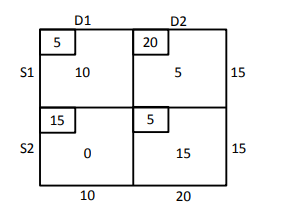
\includegraphics[width=0.75\columnwidth]{chapters/10/7/2/4/figs/fig.png}
 \end{center}
\caption{}
\label{fig:10/7/2/4Fig1}
\end{figure}
\fi

\item Find the position vector of the mid point of the vector joining the points $\vec{P}$(2, 3, 4)
and $\vec{Q}$(4, 1, –2).
\\
\solution
		\begin{enumerate}[label=\thesubsection.\arabic*,ref=\thesubsection.\theenumi]
\item Find the coordinates of the point which divides the join of $(-1,7) $ and $ (4,-3)$ in the ratio 2:3.
	\\
		\solution
	\input{chapters/10/7/2/1/section.tex}
\item Find the coordinates of the point $\vec{R}$ on the line segment joining the points $\vec{P}(-1,3)$ and $\vec{Q}(2,5)$ such that $PR=\frac{3}{5}PQ$.
\item Find the ratio in which the point $\vec{P}\brak{\frac{3}{4},\frac{5}{12}}$ divides the line segment joining the points $\vec{A}\brak{\frac{1}{2},\frac{3}{2}}$ and $ \vec{B}(2,-5)$.
\item Find the coordinates of the point which divides the line segment joining the points $(4,-3)$ and $(8,5)$ in the ratio $3:1$ internally.
\item Find the coordinates of the point $\vec{P}$ on $AD$ such that $AP : PD = 2 : 1$.
\item If the point $\vec{P} (2, 1)$ lies on the line segment joining points $\vec{A} (4, 2)$  and $ \vec{B} (8, 4)$,
then
\begin{enumerate}
	\item $AP =\frac{1}{3}{AB}$ 
\item ${AP}={PE}$
\item ${PB}=\frac{1}{3}{AB}$
\item${AP}=\frac{1}{2}{AB}$
 \end{enumerate}
\item Find the ratio in which the line segment joining the points $(-3,10)$  and  $(6,-8)$  is divided by $ (-1,6)$.
	\\
		\solution
	\input{chapters/10/7/2/4/section.tex}
\item Find the position vector of the mid point of the vector joining the points $\vec{P}$(2, 3, 4)
and $\vec{Q}$(4, 1, –2).
\\
\solution
		\input{chapters/12/10/2/16/section.tex}
\item Let $\vec{A}(4, 2), \vec{B}(6, 5)$  and $ \vec{C}(1, 4)$ be the vertices of $\triangle ABC$.
\begin{enumerate}
\item If $\vec{A}$ and  $\vec{B}$ are $(-2,-2)$ and  $(2,-4)$, respectively, find the coordinates of $\vec{P}$ such that $AP= \frac {3}{7}AB$  and $ \vec{P}$ lies on the line segment $AB$.
	\\
		\solution
	\input{chapters/10/7/2/8/section.tex}
\item Find the coordinates of the points which divide the line segment joining $A(-2,2)$  and  $\vec{B}(2,8)$ into four equal parts.
	\\
		\solution
	\input{chapters/10/7/2/9/section.tex}
\item In what ratio does the point $(-4,6)$ divide the line segment joining the points $\vec{A}(-6,0)$ and $\vec{B}(3,-8)$?
\item Given that $\vec{P}(3,2,-4), \vec{Q}(5,4,-6)$ and $\vec{R}(9,8,-10)$ are collinear. Find the ratio in which $\vec{Q}$ divides $PR$.
\item Points $\vec{A}(-6,10),\vec{B}(-4,6)$  and  $\vec{C}(3,-8)$ are collinear such that $AB=  \frac{2}{9}AC$.
\item The point which divides the line segment joining the points $\vec{P} (7, –6) $  and  $\vec{Q}(3, 4)$ in the 
ratio 1 : 2 internally lies in  which quadrant?
\item Find the coordinates of the points of trisection of the line segment joining $(4,-1)$  and  $(-2,3)$.
	\\
		\solution
	\input{chapters/10/7/2/2/section.tex}
\item Find the coordinates of the points which trisect the line segment joining the points $\vec{P}(4,2,-6)$ and $\vec{Q}(10,-16,6)$.
\item Find the coordinates of the points of trisection (i.e. points dividing to three equal parts) of the line segment joining the points $\vec{A}(2,-2)$ and $\vec{B}(-7,4)$.
\item Point $\vec{P}(5,-3)$ is one of the two points of trisection of line segment joining the points $\vec{A}(7,-2)$ and $\vec{B}(1,-5)$
\item Find the position vector of a point $\vec{R}$ which divides the line joining two points $\vec{P}$
and $\vec{Q}$ whose position vectors are $\hat{i}+2\hat{j}-\hat{k}$ and $-\hat{i}+\hat{j}+\hat{k}$ respectively, in the
ratio 2 : 1
\begin{enumerate}
    \item  internally
    \item  externally
\end{enumerate}
%\solution
%		\input{chapters/12/10/2/15/section.tex}
\item Find the coordinates of the point which divides the line segment joining the points which divides the line segment joining  the points $(-2,3,5)$ and $(1,-4,6)$ in the ratio 
\begin{enumerate}
\item $2:3$ internally,
\item $2:3$ externally
\end{enumerate}
\item Find the coordinates of the point which divides the line segment joining the points $(1,-2,3)$ and $(3,4,-5)$ in the ratio $2:3$
\begin{enumerate}
\item internally, and
\item externally
\end{enumerate}
\item Consider two points $\vec{P}$ and $\vec{Q}$ with position vectors $\overrightarrow{OP} = 3\overrightarrow{a}-2\overrightarrow{b}$ and $\overrightarrow{OQ}=\overrightarrow{a}+\overrightarrow{b}$. Find the position vector of a point $\vec{R}$ which divides the line joining $\vec{P}$ and $\vec{Q}$ in the ratio $2:1$, 
\begin{enumerate}
\item internally, and 
\item externally.
\end{enumerate}
\item The median from $\vec{A}$ meets $BC$ at $\vec{D}$. Find the coordinates of the point $\vec{D}$.
\item Find the coordinates of points $\vec{Q}$ and $\vec{R}$ on medians $BE$ and $CF$ respectively such that $BQ : QE = 2 : 1$  and  $CR : RF = 2 : 1$.
\item What do you observe?
\item If $\vec{A}, \vec{B}$ and $\vec{C}$  are the vertices of $\triangle ABC$, find the coordinates of the centroid of the triangle.
\end{enumerate}
\solution
	\input{chapters/10/7/4/7/section.tex}
\item If $\vec{P}(9a-2,-b)$ divides line segment joining $\vec{A}(3a+1,-3)$ and $\vec{B}(8a,5)$ in the ratio 3:1, find the values of $a$ and $b$.
\item Find the position vector of a point $\vec{R}$ which divides the line joining two points $\vec{P}$ and $\vec{Q}$ whose position vectors are $2\vec{a}+\vec{b}$ and $\vec{a}-3\vec{b}$ externally in the ratio $1:2$.
\item The position vector of the point which divides the join of points 2$\vec{a}$-3$\vec{b}$ $\text{and}$ $\vec{a}+\vec{b}$ in the ratio 3:1 is \rule{1cm}{0.1pt}.
\item If $\vec{a}$ and $\vec{b}$ are the postion vectors of $\vec{A}$ and $\vec{B}$, respectively, find the position vector of a point $\vec{C}$ in $BA$ produced such that $BC=1.5BA$.
\item Find the position vector of a point $\vec{R}$ which divides the line joining two points $\vec{P}$ and $\vec{Q}$ whose position vectors are $(2\vec{a}+\vec{b})$ and $(\vec{a}-3\vec{b})$
externally in the ratio 1 : 2. Also, show that $\vec{P}$ is the mid point of the line segment $RQ$.
\end{enumerate}

\item Let $\vec{A}(4, 2), \vec{B}(6, 5)$  and $ \vec{C}(1, 4)$ be the vertices of $\triangle ABC$.
\begin{enumerate}
\item If $\vec{A}$ and  $\vec{B}$ are $(-2,-2)$ and  $(2,-4)$, respectively, find the coordinates of $\vec{P}$ such that $AP= \frac {3}{7}AB$  and $ \vec{P}$ lies on the line segment $AB$.
	\\
		\solution
	\begin{enumerate}[label=\thesubsection.\arabic*,ref=\thesubsection.\theenumi]
\item Find the coordinates of the point which divides the join of $(-1,7) $ and $ (4,-3)$ in the ratio 2:3.
	\\
		\solution
	\input{chapters/10/7/2/1/section.tex}
\item Find the coordinates of the point $\vec{R}$ on the line segment joining the points $\vec{P}(-1,3)$ and $\vec{Q}(2,5)$ such that $PR=\frac{3}{5}PQ$.
\item Find the ratio in which the point $\vec{P}\brak{\frac{3}{4},\frac{5}{12}}$ divides the line segment joining the points $\vec{A}\brak{\frac{1}{2},\frac{3}{2}}$ and $ \vec{B}(2,-5)$.
\item Find the coordinates of the point which divides the line segment joining the points $(4,-3)$ and $(8,5)$ in the ratio $3:1$ internally.
\item Find the coordinates of the point $\vec{P}$ on $AD$ such that $AP : PD = 2 : 1$.
\item If the point $\vec{P} (2, 1)$ lies on the line segment joining points $\vec{A} (4, 2)$  and $ \vec{B} (8, 4)$,
then
\begin{enumerate}
	\item $AP =\frac{1}{3}{AB}$ 
\item ${AP}={PE}$
\item ${PB}=\frac{1}{3}{AB}$
\item${AP}=\frac{1}{2}{AB}$
 \end{enumerate}
\item Find the ratio in which the line segment joining the points $(-3,10)$  and  $(6,-8)$  is divided by $ (-1,6)$.
	\\
		\solution
	\input{chapters/10/7/2/4/section.tex}
\item Find the position vector of the mid point of the vector joining the points $\vec{P}$(2, 3, 4)
and $\vec{Q}$(4, 1, –2).
\\
\solution
		\input{chapters/12/10/2/16/section.tex}
\item Let $\vec{A}(4, 2), \vec{B}(6, 5)$  and $ \vec{C}(1, 4)$ be the vertices of $\triangle ABC$.
\begin{enumerate}
\item If $\vec{A}$ and  $\vec{B}$ are $(-2,-2)$ and  $(2,-4)$, respectively, find the coordinates of $\vec{P}$ such that $AP= \frac {3}{7}AB$  and $ \vec{P}$ lies on the line segment $AB$.
	\\
		\solution
	\input{chapters/10/7/2/8/section.tex}
\item Find the coordinates of the points which divide the line segment joining $A(-2,2)$  and  $\vec{B}(2,8)$ into four equal parts.
	\\
		\solution
	\input{chapters/10/7/2/9/section.tex}
\item In what ratio does the point $(-4,6)$ divide the line segment joining the points $\vec{A}(-6,0)$ and $\vec{B}(3,-8)$?
\item Given that $\vec{P}(3,2,-4), \vec{Q}(5,4,-6)$ and $\vec{R}(9,8,-10)$ are collinear. Find the ratio in which $\vec{Q}$ divides $PR$.
\item Points $\vec{A}(-6,10),\vec{B}(-4,6)$  and  $\vec{C}(3,-8)$ are collinear such that $AB=  \frac{2}{9}AC$.
\item The point which divides the line segment joining the points $\vec{P} (7, –6) $  and  $\vec{Q}(3, 4)$ in the 
ratio 1 : 2 internally lies in  which quadrant?
\item Find the coordinates of the points of trisection of the line segment joining $(4,-1)$  and  $(-2,3)$.
	\\
		\solution
	\input{chapters/10/7/2/2/section.tex}
\item Find the coordinates of the points which trisect the line segment joining the points $\vec{P}(4,2,-6)$ and $\vec{Q}(10,-16,6)$.
\item Find the coordinates of the points of trisection (i.e. points dividing to three equal parts) of the line segment joining the points $\vec{A}(2,-2)$ and $\vec{B}(-7,4)$.
\item Point $\vec{P}(5,-3)$ is one of the two points of trisection of line segment joining the points $\vec{A}(7,-2)$ and $\vec{B}(1,-5)$
\item Find the position vector of a point $\vec{R}$ which divides the line joining two points $\vec{P}$
and $\vec{Q}$ whose position vectors are $\hat{i}+2\hat{j}-\hat{k}$ and $-\hat{i}+\hat{j}+\hat{k}$ respectively, in the
ratio 2 : 1
\begin{enumerate}
    \item  internally
    \item  externally
\end{enumerate}
%\solution
%		\input{chapters/12/10/2/15/section.tex}
\item Find the coordinates of the point which divides the line segment joining the points which divides the line segment joining  the points $(-2,3,5)$ and $(1,-4,6)$ in the ratio 
\begin{enumerate}
\item $2:3$ internally,
\item $2:3$ externally
\end{enumerate}
\item Find the coordinates of the point which divides the line segment joining the points $(1,-2,3)$ and $(3,4,-5)$ in the ratio $2:3$
\begin{enumerate}
\item internally, and
\item externally
\end{enumerate}
\item Consider two points $\vec{P}$ and $\vec{Q}$ with position vectors $\overrightarrow{OP} = 3\overrightarrow{a}-2\overrightarrow{b}$ and $\overrightarrow{OQ}=\overrightarrow{a}+\overrightarrow{b}$. Find the position vector of a point $\vec{R}$ which divides the line joining $\vec{P}$ and $\vec{Q}$ in the ratio $2:1$, 
\begin{enumerate}
\item internally, and 
\item externally.
\end{enumerate}
\item The median from $\vec{A}$ meets $BC$ at $\vec{D}$. Find the coordinates of the point $\vec{D}$.
\item Find the coordinates of points $\vec{Q}$ and $\vec{R}$ on medians $BE$ and $CF$ respectively such that $BQ : QE = 2 : 1$  and  $CR : RF = 2 : 1$.
\item What do you observe?
\item If $\vec{A}, \vec{B}$ and $\vec{C}$  are the vertices of $\triangle ABC$, find the coordinates of the centroid of the triangle.
\end{enumerate}
\solution
	\input{chapters/10/7/4/7/section.tex}
\item If $\vec{P}(9a-2,-b)$ divides line segment joining $\vec{A}(3a+1,-3)$ and $\vec{B}(8a,5)$ in the ratio 3:1, find the values of $a$ and $b$.
\item Find the position vector of a point $\vec{R}$ which divides the line joining two points $\vec{P}$ and $\vec{Q}$ whose position vectors are $2\vec{a}+\vec{b}$ and $\vec{a}-3\vec{b}$ externally in the ratio $1:2$.
\item The position vector of the point which divides the join of points 2$\vec{a}$-3$\vec{b}$ $\text{and}$ $\vec{a}+\vec{b}$ in the ratio 3:1 is \rule{1cm}{0.1pt}.
\item If $\vec{a}$ and $\vec{b}$ are the postion vectors of $\vec{A}$ and $\vec{B}$, respectively, find the position vector of a point $\vec{C}$ in $BA$ produced such that $BC=1.5BA$.
\item Find the position vector of a point $\vec{R}$ which divides the line joining two points $\vec{P}$ and $\vec{Q}$ whose position vectors are $(2\vec{a}+\vec{b})$ and $(\vec{a}-3\vec{b})$
externally in the ratio 1 : 2. Also, show that $\vec{P}$ is the mid point of the line segment $RQ$.
\end{enumerate}

\item Find the coordinates of the points which divide the line segment joining $A(-2,2)$  and  $\vec{B}(2,8)$ into four equal parts.
	\\
		\solution
	\begin{enumerate}[label=\thesubsection.\arabic*,ref=\thesubsection.\theenumi]
\item Find the coordinates of the point which divides the join of $(-1,7) $ and $ (4,-3)$ in the ratio 2:3.
	\\
		\solution
	\input{chapters/10/7/2/1/section.tex}
\item Find the coordinates of the point $\vec{R}$ on the line segment joining the points $\vec{P}(-1,3)$ and $\vec{Q}(2,5)$ such that $PR=\frac{3}{5}PQ$.
\item Find the ratio in which the point $\vec{P}\brak{\frac{3}{4},\frac{5}{12}}$ divides the line segment joining the points $\vec{A}\brak{\frac{1}{2},\frac{3}{2}}$ and $ \vec{B}(2,-5)$.
\item Find the coordinates of the point which divides the line segment joining the points $(4,-3)$ and $(8,5)$ in the ratio $3:1$ internally.
\item Find the coordinates of the point $\vec{P}$ on $AD$ such that $AP : PD = 2 : 1$.
\item If the point $\vec{P} (2, 1)$ lies on the line segment joining points $\vec{A} (4, 2)$  and $ \vec{B} (8, 4)$,
then
\begin{enumerate}
	\item $AP =\frac{1}{3}{AB}$ 
\item ${AP}={PE}$
\item ${PB}=\frac{1}{3}{AB}$
\item${AP}=\frac{1}{2}{AB}$
 \end{enumerate}
\item Find the ratio in which the line segment joining the points $(-3,10)$  and  $(6,-8)$  is divided by $ (-1,6)$.
	\\
		\solution
	\input{chapters/10/7/2/4/section.tex}
\item Find the position vector of the mid point of the vector joining the points $\vec{P}$(2, 3, 4)
and $\vec{Q}$(4, 1, –2).
\\
\solution
		\input{chapters/12/10/2/16/section.tex}
\item Let $\vec{A}(4, 2), \vec{B}(6, 5)$  and $ \vec{C}(1, 4)$ be the vertices of $\triangle ABC$.
\begin{enumerate}
\item If $\vec{A}$ and  $\vec{B}$ are $(-2,-2)$ and  $(2,-4)$, respectively, find the coordinates of $\vec{P}$ such that $AP= \frac {3}{7}AB$  and $ \vec{P}$ lies on the line segment $AB$.
	\\
		\solution
	\input{chapters/10/7/2/8/section.tex}
\item Find the coordinates of the points which divide the line segment joining $A(-2,2)$  and  $\vec{B}(2,8)$ into four equal parts.
	\\
		\solution
	\input{chapters/10/7/2/9/section.tex}
\item In what ratio does the point $(-4,6)$ divide the line segment joining the points $\vec{A}(-6,0)$ and $\vec{B}(3,-8)$?
\item Given that $\vec{P}(3,2,-4), \vec{Q}(5,4,-6)$ and $\vec{R}(9,8,-10)$ are collinear. Find the ratio in which $\vec{Q}$ divides $PR$.
\item Points $\vec{A}(-6,10),\vec{B}(-4,6)$  and  $\vec{C}(3,-8)$ are collinear such that $AB=  \frac{2}{9}AC$.
\item The point which divides the line segment joining the points $\vec{P} (7, –6) $  and  $\vec{Q}(3, 4)$ in the 
ratio 1 : 2 internally lies in  which quadrant?
\item Find the coordinates of the points of trisection of the line segment joining $(4,-1)$  and  $(-2,3)$.
	\\
		\solution
	\input{chapters/10/7/2/2/section.tex}
\item Find the coordinates of the points which trisect the line segment joining the points $\vec{P}(4,2,-6)$ and $\vec{Q}(10,-16,6)$.
\item Find the coordinates of the points of trisection (i.e. points dividing to three equal parts) of the line segment joining the points $\vec{A}(2,-2)$ and $\vec{B}(-7,4)$.
\item Point $\vec{P}(5,-3)$ is one of the two points of trisection of line segment joining the points $\vec{A}(7,-2)$ and $\vec{B}(1,-5)$
\item Find the position vector of a point $\vec{R}$ which divides the line joining two points $\vec{P}$
and $\vec{Q}$ whose position vectors are $\hat{i}+2\hat{j}-\hat{k}$ and $-\hat{i}+\hat{j}+\hat{k}$ respectively, in the
ratio 2 : 1
\begin{enumerate}
    \item  internally
    \item  externally
\end{enumerate}
%\solution
%		\input{chapters/12/10/2/15/section.tex}
\item Find the coordinates of the point which divides the line segment joining the points which divides the line segment joining  the points $(-2,3,5)$ and $(1,-4,6)$ in the ratio 
\begin{enumerate}
\item $2:3$ internally,
\item $2:3$ externally
\end{enumerate}
\item Find the coordinates of the point which divides the line segment joining the points $(1,-2,3)$ and $(3,4,-5)$ in the ratio $2:3$
\begin{enumerate}
\item internally, and
\item externally
\end{enumerate}
\item Consider two points $\vec{P}$ and $\vec{Q}$ with position vectors $\overrightarrow{OP} = 3\overrightarrow{a}-2\overrightarrow{b}$ and $\overrightarrow{OQ}=\overrightarrow{a}+\overrightarrow{b}$. Find the position vector of a point $\vec{R}$ which divides the line joining $\vec{P}$ and $\vec{Q}$ in the ratio $2:1$, 
\begin{enumerate}
\item internally, and 
\item externally.
\end{enumerate}
\item The median from $\vec{A}$ meets $BC$ at $\vec{D}$. Find the coordinates of the point $\vec{D}$.
\item Find the coordinates of points $\vec{Q}$ and $\vec{R}$ on medians $BE$ and $CF$ respectively such that $BQ : QE = 2 : 1$  and  $CR : RF = 2 : 1$.
\item What do you observe?
\item If $\vec{A}, \vec{B}$ and $\vec{C}$  are the vertices of $\triangle ABC$, find the coordinates of the centroid of the triangle.
\end{enumerate}
\solution
	\input{chapters/10/7/4/7/section.tex}
\item If $\vec{P}(9a-2,-b)$ divides line segment joining $\vec{A}(3a+1,-3)$ and $\vec{B}(8a,5)$ in the ratio 3:1, find the values of $a$ and $b$.
\item Find the position vector of a point $\vec{R}$ which divides the line joining two points $\vec{P}$ and $\vec{Q}$ whose position vectors are $2\vec{a}+\vec{b}$ and $\vec{a}-3\vec{b}$ externally in the ratio $1:2$.
\item The position vector of the point which divides the join of points 2$\vec{a}$-3$\vec{b}$ $\text{and}$ $\vec{a}+\vec{b}$ in the ratio 3:1 is \rule{1cm}{0.1pt}.
\item If $\vec{a}$ and $\vec{b}$ are the postion vectors of $\vec{A}$ and $\vec{B}$, respectively, find the position vector of a point $\vec{C}$ in $BA$ produced such that $BC=1.5BA$.
\item Find the position vector of a point $\vec{R}$ which divides the line joining two points $\vec{P}$ and $\vec{Q}$ whose position vectors are $(2\vec{a}+\vec{b})$ and $(\vec{a}-3\vec{b})$
externally in the ratio 1 : 2. Also, show that $\vec{P}$ is the mid point of the line segment $RQ$.
\end{enumerate}

\item In what ratio does the point $(-4,6)$ divide the line segment joining the points $\vec{A}(-6,0)$ and $\vec{B}(3,-8)$?
\item Given that $\vec{P}(3,2,-4), \vec{Q}(5,4,-6)$ and $\vec{R}(9,8,-10)$ are collinear. Find the ratio in which $\vec{Q}$ divides $PR$.
\item Points $\vec{A}(-6,10),\vec{B}(-4,6)$  and  $\vec{C}(3,-8)$ are collinear such that $AB=  \frac{2}{9}AC$.
\item The point which divides the line segment joining the points $\vec{P} (7, –6) $  and  $\vec{Q}(3, 4)$ in the 
ratio 1 : 2 internally lies in  which quadrant?
\item Find the coordinates of the points of trisection of the line segment joining $(4,-1)$  and  $(-2,3)$.
	\\
		\solution
	Using section formula,
\begin{align}
\vec{R}=\frac{1}{1+\frac{1}{2}}\brak{\myvec{4\\-1}+\frac{1}{2}\myvec{-2\\3}}
=\myvec{2\\ \frac{1}{3}}\\
\vec{S}=\frac{1}{1+\frac{2}{1}}\brak{\myvec{4\\-1}+\frac{2}{1}\myvec{-2\\3}}
=\myvec{0\\ \frac{5}{3}}
\end{align}
which are the desired points of trisection.
\iffalse
See
		\figref{fig:chapters/10/7/2/2/Figure}
\begin{figure}[H]
\centering
\includegraphics[width=0.75\columnwidth]{chapters/10/7/2/2/figs/dj.pdf}
\caption{}
		\label{fig:chapters/10/7/2/2/Figure}
\end{figure}
\fi

\item Find the coordinates of the points which trisect the line segment joining the points $\vec{P}(4,2,-6)$ and $\vec{Q}(10,-16,6)$.
\item Find the coordinates of the points of trisection (i.e. points dividing to three equal parts) of the line segment joining the points $\vec{A}(2,-2)$ and $\vec{B}(-7,4)$.
\item Point $\vec{P}(5,-3)$ is one of the two points of trisection of line segment joining the points $\vec{A}(7,-2)$ and $\vec{B}(1,-5)$
\item Find the position vector of a point $\vec{R}$ which divides the line joining two points $\vec{P}$
and $\vec{Q}$ whose position vectors are $\hat{i}+2\hat{j}-\hat{k}$ and $-\hat{i}+\hat{j}+\hat{k}$ respectively, in the
ratio 2 : 1
\begin{enumerate}
    \item  internally
    \item  externally
\end{enumerate}
%\solution
%		\begin{enumerate}[label=\thesubsection.\arabic*,ref=\thesubsection.\theenumi]
\item Find the coordinates of the point which divides the join of $(-1,7) $ and $ (4,-3)$ in the ratio 2:3.
	\\
		\solution
	\input{chapters/10/7/2/1/section.tex}
\item Find the coordinates of the point $\vec{R}$ on the line segment joining the points $\vec{P}(-1,3)$ and $\vec{Q}(2,5)$ such that $PR=\frac{3}{5}PQ$.
\item Find the ratio in which the point $\vec{P}\brak{\frac{3}{4},\frac{5}{12}}$ divides the line segment joining the points $\vec{A}\brak{\frac{1}{2},\frac{3}{2}}$ and $ \vec{B}(2,-5)$.
\item Find the coordinates of the point which divides the line segment joining the points $(4,-3)$ and $(8,5)$ in the ratio $3:1$ internally.
\item Find the coordinates of the point $\vec{P}$ on $AD$ such that $AP : PD = 2 : 1$.
\item If the point $\vec{P} (2, 1)$ lies on the line segment joining points $\vec{A} (4, 2)$  and $ \vec{B} (8, 4)$,
then
\begin{enumerate}
	\item $AP =\frac{1}{3}{AB}$ 
\item ${AP}={PE}$
\item ${PB}=\frac{1}{3}{AB}$
\item${AP}=\frac{1}{2}{AB}$
 \end{enumerate}
\item Find the ratio in which the line segment joining the points $(-3,10)$  and  $(6,-8)$  is divided by $ (-1,6)$.
	\\
		\solution
	\input{chapters/10/7/2/4/section.tex}
\item Find the position vector of the mid point of the vector joining the points $\vec{P}$(2, 3, 4)
and $\vec{Q}$(4, 1, –2).
\\
\solution
		\input{chapters/12/10/2/16/section.tex}
\item Let $\vec{A}(4, 2), \vec{B}(6, 5)$  and $ \vec{C}(1, 4)$ be the vertices of $\triangle ABC$.
\begin{enumerate}
\item If $\vec{A}$ and  $\vec{B}$ are $(-2,-2)$ and  $(2,-4)$, respectively, find the coordinates of $\vec{P}$ such that $AP= \frac {3}{7}AB$  and $ \vec{P}$ lies on the line segment $AB$.
	\\
		\solution
	\input{chapters/10/7/2/8/section.tex}
\item Find the coordinates of the points which divide the line segment joining $A(-2,2)$  and  $\vec{B}(2,8)$ into four equal parts.
	\\
		\solution
	\input{chapters/10/7/2/9/section.tex}
\item In what ratio does the point $(-4,6)$ divide the line segment joining the points $\vec{A}(-6,0)$ and $\vec{B}(3,-8)$?
\item Given that $\vec{P}(3,2,-4), \vec{Q}(5,4,-6)$ and $\vec{R}(9,8,-10)$ are collinear. Find the ratio in which $\vec{Q}$ divides $PR$.
\item Points $\vec{A}(-6,10),\vec{B}(-4,6)$  and  $\vec{C}(3,-8)$ are collinear such that $AB=  \frac{2}{9}AC$.
\item The point which divides the line segment joining the points $\vec{P} (7, –6) $  and  $\vec{Q}(3, 4)$ in the 
ratio 1 : 2 internally lies in  which quadrant?
\item Find the coordinates of the points of trisection of the line segment joining $(4,-1)$  and  $(-2,3)$.
	\\
		\solution
	\input{chapters/10/7/2/2/section.tex}
\item Find the coordinates of the points which trisect the line segment joining the points $\vec{P}(4,2,-6)$ and $\vec{Q}(10,-16,6)$.
\item Find the coordinates of the points of trisection (i.e. points dividing to three equal parts) of the line segment joining the points $\vec{A}(2,-2)$ and $\vec{B}(-7,4)$.
\item Point $\vec{P}(5,-3)$ is one of the two points of trisection of line segment joining the points $\vec{A}(7,-2)$ and $\vec{B}(1,-5)$
\item Find the position vector of a point $\vec{R}$ which divides the line joining two points $\vec{P}$
and $\vec{Q}$ whose position vectors are $\hat{i}+2\hat{j}-\hat{k}$ and $-\hat{i}+\hat{j}+\hat{k}$ respectively, in the
ratio 2 : 1
\begin{enumerate}
    \item  internally
    \item  externally
\end{enumerate}
%\solution
%		\input{chapters/12/10/2/15/section.tex}
\item Find the coordinates of the point which divides the line segment joining the points which divides the line segment joining  the points $(-2,3,5)$ and $(1,-4,6)$ in the ratio 
\begin{enumerate}
\item $2:3$ internally,
\item $2:3$ externally
\end{enumerate}
\item Find the coordinates of the point which divides the line segment joining the points $(1,-2,3)$ and $(3,4,-5)$ in the ratio $2:3$
\begin{enumerate}
\item internally, and
\item externally
\end{enumerate}
\item Consider two points $\vec{P}$ and $\vec{Q}$ with position vectors $\overrightarrow{OP} = 3\overrightarrow{a}-2\overrightarrow{b}$ and $\overrightarrow{OQ}=\overrightarrow{a}+\overrightarrow{b}$. Find the position vector of a point $\vec{R}$ which divides the line joining $\vec{P}$ and $\vec{Q}$ in the ratio $2:1$, 
\begin{enumerate}
\item internally, and 
\item externally.
\end{enumerate}
\item The median from $\vec{A}$ meets $BC$ at $\vec{D}$. Find the coordinates of the point $\vec{D}$.
\item Find the coordinates of points $\vec{Q}$ and $\vec{R}$ on medians $BE$ and $CF$ respectively such that $BQ : QE = 2 : 1$  and  $CR : RF = 2 : 1$.
\item What do you observe?
\item If $\vec{A}, \vec{B}$ and $\vec{C}$  are the vertices of $\triangle ABC$, find the coordinates of the centroid of the triangle.
\end{enumerate}
\solution
	\input{chapters/10/7/4/7/section.tex}
\item If $\vec{P}(9a-2,-b)$ divides line segment joining $\vec{A}(3a+1,-3)$ and $\vec{B}(8a,5)$ in the ratio 3:1, find the values of $a$ and $b$.
\item Find the position vector of a point $\vec{R}$ which divides the line joining two points $\vec{P}$ and $\vec{Q}$ whose position vectors are $2\vec{a}+\vec{b}$ and $\vec{a}-3\vec{b}$ externally in the ratio $1:2$.
\item The position vector of the point which divides the join of points 2$\vec{a}$-3$\vec{b}$ $\text{and}$ $\vec{a}+\vec{b}$ in the ratio 3:1 is \rule{1cm}{0.1pt}.
\item If $\vec{a}$ and $\vec{b}$ are the postion vectors of $\vec{A}$ and $\vec{B}$, respectively, find the position vector of a point $\vec{C}$ in $BA$ produced such that $BC=1.5BA$.
\item Find the position vector of a point $\vec{R}$ which divides the line joining two points $\vec{P}$ and $\vec{Q}$ whose position vectors are $(2\vec{a}+\vec{b})$ and $(\vec{a}-3\vec{b})$
externally in the ratio 1 : 2. Also, show that $\vec{P}$ is the mid point of the line segment $RQ$.
\end{enumerate}

\item Find the coordinates of the point which divides the line segment joining the points which divides the line segment joining  the points $(-2,3,5)$ and $(1,-4,6)$ in the ratio 
\begin{enumerate}
\item $2:3$ internally,
\item $2:3$ externally
\end{enumerate}
\item Find the coordinates of the point which divides the line segment joining the points $(1,-2,3)$ and $(3,4,-5)$ in the ratio $2:3$
\begin{enumerate}
\item internally, and
\item externally
\end{enumerate}
\item Consider two points $\vec{P}$ and $\vec{Q}$ with position vectors $\overrightarrow{OP} = 3\overrightarrow{a}-2\overrightarrow{b}$ and $\overrightarrow{OQ}=\overrightarrow{a}+\overrightarrow{b}$. Find the position vector of a point $\vec{R}$ which divides the line joining $\vec{P}$ and $\vec{Q}$ in the ratio $2:1$, 
\begin{enumerate}
\item internally, and 
\item externally.
\end{enumerate}
\item The median from $\vec{A}$ meets $BC$ at $\vec{D}$. Find the coordinates of the point $\vec{D}$.
\item Find the coordinates of points $\vec{Q}$ and $\vec{R}$ on medians $BE$ and $CF$ respectively such that $BQ : QE = 2 : 1$  and  $CR : RF = 2 : 1$.
\item What do you observe?
\item If $\vec{A}, \vec{B}$ and $\vec{C}$  are the vertices of $\triangle ABC$, find the coordinates of the centroid of the triangle.
\end{enumerate}
\solution
	\begin{enumerate}[label=\thesubsection.\arabic*,ref=\thesubsection.\theenumi]
\item Find the coordinates of the point which divides the join of $(-1,7) $ and $ (4,-3)$ in the ratio 2:3.
	\\
		\solution
	\input{chapters/10/7/2/1/section.tex}
\item Find the coordinates of the point $\vec{R}$ on the line segment joining the points $\vec{P}(-1,3)$ and $\vec{Q}(2,5)$ such that $PR=\frac{3}{5}PQ$.
\item Find the ratio in which the point $\vec{P}\brak{\frac{3}{4},\frac{5}{12}}$ divides the line segment joining the points $\vec{A}\brak{\frac{1}{2},\frac{3}{2}}$ and $ \vec{B}(2,-5)$.
\item Find the coordinates of the point which divides the line segment joining the points $(4,-3)$ and $(8,5)$ in the ratio $3:1$ internally.
\item Find the coordinates of the point $\vec{P}$ on $AD$ such that $AP : PD = 2 : 1$.
\item If the point $\vec{P} (2, 1)$ lies on the line segment joining points $\vec{A} (4, 2)$  and $ \vec{B} (8, 4)$,
then
\begin{enumerate}
	\item $AP =\frac{1}{3}{AB}$ 
\item ${AP}={PE}$
\item ${PB}=\frac{1}{3}{AB}$
\item${AP}=\frac{1}{2}{AB}$
 \end{enumerate}
\item Find the ratio in which the line segment joining the points $(-3,10)$  and  $(6,-8)$  is divided by $ (-1,6)$.
	\\
		\solution
	\input{chapters/10/7/2/4/section.tex}
\item Find the position vector of the mid point of the vector joining the points $\vec{P}$(2, 3, 4)
and $\vec{Q}$(4, 1, –2).
\\
\solution
		\input{chapters/12/10/2/16/section.tex}
\item Let $\vec{A}(4, 2), \vec{B}(6, 5)$  and $ \vec{C}(1, 4)$ be the vertices of $\triangle ABC$.
\begin{enumerate}
\item If $\vec{A}$ and  $\vec{B}$ are $(-2,-2)$ and  $(2,-4)$, respectively, find the coordinates of $\vec{P}$ such that $AP= \frac {3}{7}AB$  and $ \vec{P}$ lies on the line segment $AB$.
	\\
		\solution
	\input{chapters/10/7/2/8/section.tex}
\item Find the coordinates of the points which divide the line segment joining $A(-2,2)$  and  $\vec{B}(2,8)$ into four equal parts.
	\\
		\solution
	\input{chapters/10/7/2/9/section.tex}
\item In what ratio does the point $(-4,6)$ divide the line segment joining the points $\vec{A}(-6,0)$ and $\vec{B}(3,-8)$?
\item Given that $\vec{P}(3,2,-4), \vec{Q}(5,4,-6)$ and $\vec{R}(9,8,-10)$ are collinear. Find the ratio in which $\vec{Q}$ divides $PR$.
\item Points $\vec{A}(-6,10),\vec{B}(-4,6)$  and  $\vec{C}(3,-8)$ are collinear such that $AB=  \frac{2}{9}AC$.
\item The point which divides the line segment joining the points $\vec{P} (7, –6) $  and  $\vec{Q}(3, 4)$ in the 
ratio 1 : 2 internally lies in  which quadrant?
\item Find the coordinates of the points of trisection of the line segment joining $(4,-1)$  and  $(-2,3)$.
	\\
		\solution
	\input{chapters/10/7/2/2/section.tex}
\item Find the coordinates of the points which trisect the line segment joining the points $\vec{P}(4,2,-6)$ and $\vec{Q}(10,-16,6)$.
\item Find the coordinates of the points of trisection (i.e. points dividing to three equal parts) of the line segment joining the points $\vec{A}(2,-2)$ and $\vec{B}(-7,4)$.
\item Point $\vec{P}(5,-3)$ is one of the two points of trisection of line segment joining the points $\vec{A}(7,-2)$ and $\vec{B}(1,-5)$
\item Find the position vector of a point $\vec{R}$ which divides the line joining two points $\vec{P}$
and $\vec{Q}$ whose position vectors are $\hat{i}+2\hat{j}-\hat{k}$ and $-\hat{i}+\hat{j}+\hat{k}$ respectively, in the
ratio 2 : 1
\begin{enumerate}
    \item  internally
    \item  externally
\end{enumerate}
%\solution
%		\input{chapters/12/10/2/15/section.tex}
\item Find the coordinates of the point which divides the line segment joining the points which divides the line segment joining  the points $(-2,3,5)$ and $(1,-4,6)$ in the ratio 
\begin{enumerate}
\item $2:3$ internally,
\item $2:3$ externally
\end{enumerate}
\item Find the coordinates of the point which divides the line segment joining the points $(1,-2,3)$ and $(3,4,-5)$ in the ratio $2:3$
\begin{enumerate}
\item internally, and
\item externally
\end{enumerate}
\item Consider two points $\vec{P}$ and $\vec{Q}$ with position vectors $\overrightarrow{OP} = 3\overrightarrow{a}-2\overrightarrow{b}$ and $\overrightarrow{OQ}=\overrightarrow{a}+\overrightarrow{b}$. Find the position vector of a point $\vec{R}$ which divides the line joining $\vec{P}$ and $\vec{Q}$ in the ratio $2:1$, 
\begin{enumerate}
\item internally, and 
\item externally.
\end{enumerate}
\item The median from $\vec{A}$ meets $BC$ at $\vec{D}$. Find the coordinates of the point $\vec{D}$.
\item Find the coordinates of points $\vec{Q}$ and $\vec{R}$ on medians $BE$ and $CF$ respectively such that $BQ : QE = 2 : 1$  and  $CR : RF = 2 : 1$.
\item What do you observe?
\item If $\vec{A}, \vec{B}$ and $\vec{C}$  are the vertices of $\triangle ABC$, find the coordinates of the centroid of the triangle.
\end{enumerate}
\solution
	\input{chapters/10/7/4/7/section.tex}
\item If $\vec{P}(9a-2,-b)$ divides line segment joining $\vec{A}(3a+1,-3)$ and $\vec{B}(8a,5)$ in the ratio 3:1, find the values of $a$ and $b$.
\item Find the position vector of a point $\vec{R}$ which divides the line joining two points $\vec{P}$ and $\vec{Q}$ whose position vectors are $2\vec{a}+\vec{b}$ and $\vec{a}-3\vec{b}$ externally in the ratio $1:2$.
\item The position vector of the point which divides the join of points 2$\vec{a}$-3$\vec{b}$ $\text{and}$ $\vec{a}+\vec{b}$ in the ratio 3:1 is \rule{1cm}{0.1pt}.
\item If $\vec{a}$ and $\vec{b}$ are the postion vectors of $\vec{A}$ and $\vec{B}$, respectively, find the position vector of a point $\vec{C}$ in $BA$ produced such that $BC=1.5BA$.
\item Find the position vector of a point $\vec{R}$ which divides the line joining two points $\vec{P}$ and $\vec{Q}$ whose position vectors are $(2\vec{a}+\vec{b})$ and $(\vec{a}-3\vec{b})$
externally in the ratio 1 : 2. Also, show that $\vec{P}$ is the mid point of the line segment $RQ$.
\end{enumerate}

\item If $\vec{P}(9a-2,-b)$ divides line segment joining $\vec{A}(3a+1,-3)$ and $\vec{B}(8a,5)$ in the ratio 3:1, find the values of $a$ and $b$.
\item Find the position vector of a point $\vec{R}$ which divides the line joining two points $\vec{P}$ and $\vec{Q}$ whose position vectors are $2\vec{a}+\vec{b}$ and $\vec{a}-3\vec{b}$ externally in the ratio $1:2$.
\item The position vector of the point which divides the join of points 2$\vec{a}$-3$\vec{b}$ $\text{and}$ $\vec{a}+\vec{b}$ in the ratio 3:1 is \rule{1cm}{0.1pt}.
\item If $\vec{a}$ and $\vec{b}$ are the postion vectors of $\vec{A}$ and $\vec{B}$, respectively, find the position vector of a point $\vec{C}$ in $BA$ produced such that $BC=1.5BA$.
\item Find the position vector of a point $\vec{R}$ which divides the line joining two points $\vec{P}$ and $\vec{Q}$ whose position vectors are $(2\vec{a}+\vec{b})$ and $(\vec{a}-3\vec{b})$
externally in the ratio 1 : 2. Also, show that $\vec{P}$ is the mid point of the line segment $RQ$.
\end{enumerate}

\item In what ratio does the point $(-4,6)$ divide the line segment joining the points $\vec{A}(-6,0)$ and $\vec{B}(3,-8)$?
\item Given that $\vec{P}(3,2,-4), \vec{Q}(5,4,-6)$ and $\vec{R}(9,8,-10)$ are collinear. Find the ratio in which $\vec{Q}$ divides $PR$.
\item Points $\vec{A}(-6,10),\vec{B}(-4,6)$  and  $\vec{C}(3,-8)$ are collinear such that $AB=  \frac{2}{9}AC$.
\item The point which divides the line segment joining the points $\vec{P} (7, –6) $  and  $\vec{Q}(3, 4)$ in the 
ratio 1 : 2 internally lies in  which quadrant?
\item Find the coordinates of the points of trisection of the line segment joining $(4,-1)$  and  $(-2,3)$.
	\\
		\solution
	Using section formula,
\begin{align}
\vec{R}=\frac{1}{1+\frac{1}{2}}\brak{\myvec{4\\-1}+\frac{1}{2}\myvec{-2\\3}}
=\myvec{2\\ \frac{1}{3}}\\
\vec{S}=\frac{1}{1+\frac{2}{1}}\brak{\myvec{4\\-1}+\frac{2}{1}\myvec{-2\\3}}
=\myvec{0\\ \frac{5}{3}}
\end{align}
which are the desired points of trisection.
\iffalse
See
		\figref{fig:chapters/10/7/2/2/Figure}
\begin{figure}[H]
\centering
\includegraphics[width=0.75\columnwidth]{chapters/10/7/2/2/figs/dj.pdf}
\caption{}
		\label{fig:chapters/10/7/2/2/Figure}
\end{figure}
\fi

\item Find the coordinates of the points which trisect the line segment joining the points $\vec{P}(4,2,-6)$ and $\vec{Q}(10,-16,6)$.
\item Find the coordinates of the points of trisection (i.e. points dividing to three equal parts) of the line segment joining the points $\vec{A}(2,-2)$ and $\vec{B}(-7,4)$.
\item Point $\vec{P}(5,-3)$ is one of the two points of trisection of line segment joining the points $\vec{A}(7,-2)$ and $\vec{B}(1,-5)$
\item Find the position vector of a point $\vec{R}$ which divides the line joining two points $\vec{P}$
and $\vec{Q}$ whose position vectors are $\hat{i}+2\hat{j}-\hat{k}$ and $-\hat{i}+\hat{j}+\hat{k}$ respectively, in the
ratio 2 : 1
\begin{enumerate}
    \item  internally
    \item  externally
\end{enumerate}
%\solution
%		\begin{enumerate}[label=\thesubsection.\arabic*,ref=\thesubsection.\theenumi]
\item Find the coordinates of the point which divides the join of $(-1,7) $ and $ (4,-3)$ in the ratio 2:3.
	\\
		\solution
	\begin{enumerate}[label=\thesubsection.\arabic*,ref=\thesubsection.\theenumi]
\item Find the coordinates of the point which divides the join of $(-1,7) $ and $ (4,-3)$ in the ratio 2:3.
	\\
		\solution
	\input{chapters/10/7/2/1/section.tex}
\item Find the coordinates of the point $\vec{R}$ on the line segment joining the points $\vec{P}(-1,3)$ and $\vec{Q}(2,5)$ such that $PR=\frac{3}{5}PQ$.
\item Find the ratio in which the point $\vec{P}\brak{\frac{3}{4},\frac{5}{12}}$ divides the line segment joining the points $\vec{A}\brak{\frac{1}{2},\frac{3}{2}}$ and $ \vec{B}(2,-5)$.
\item Find the coordinates of the point which divides the line segment joining the points $(4,-3)$ and $(8,5)$ in the ratio $3:1$ internally.
\item Find the coordinates of the point $\vec{P}$ on $AD$ such that $AP : PD = 2 : 1$.
\item If the point $\vec{P} (2, 1)$ lies on the line segment joining points $\vec{A} (4, 2)$  and $ \vec{B} (8, 4)$,
then
\begin{enumerate}
	\item $AP =\frac{1}{3}{AB}$ 
\item ${AP}={PE}$
\item ${PB}=\frac{1}{3}{AB}$
\item${AP}=\frac{1}{2}{AB}$
 \end{enumerate}
\item Find the ratio in which the line segment joining the points $(-3,10)$  and  $(6,-8)$  is divided by $ (-1,6)$.
	\\
		\solution
	\input{chapters/10/7/2/4/section.tex}
\item Find the position vector of the mid point of the vector joining the points $\vec{P}$(2, 3, 4)
and $\vec{Q}$(4, 1, –2).
\\
\solution
		\input{chapters/12/10/2/16/section.tex}
\item Let $\vec{A}(4, 2), \vec{B}(6, 5)$  and $ \vec{C}(1, 4)$ be the vertices of $\triangle ABC$.
\begin{enumerate}
\item If $\vec{A}$ and  $\vec{B}$ are $(-2,-2)$ and  $(2,-4)$, respectively, find the coordinates of $\vec{P}$ such that $AP= \frac {3}{7}AB$  and $ \vec{P}$ lies on the line segment $AB$.
	\\
		\solution
	\input{chapters/10/7/2/8/section.tex}
\item Find the coordinates of the points which divide the line segment joining $A(-2,2)$  and  $\vec{B}(2,8)$ into four equal parts.
	\\
		\solution
	\input{chapters/10/7/2/9/section.tex}
\item In what ratio does the point $(-4,6)$ divide the line segment joining the points $\vec{A}(-6,0)$ and $\vec{B}(3,-8)$?
\item Given that $\vec{P}(3,2,-4), \vec{Q}(5,4,-6)$ and $\vec{R}(9,8,-10)$ are collinear. Find the ratio in which $\vec{Q}$ divides $PR$.
\item Points $\vec{A}(-6,10),\vec{B}(-4,6)$  and  $\vec{C}(3,-8)$ are collinear such that $AB=  \frac{2}{9}AC$.
\item The point which divides the line segment joining the points $\vec{P} (7, –6) $  and  $\vec{Q}(3, 4)$ in the 
ratio 1 : 2 internally lies in  which quadrant?
\item Find the coordinates of the points of trisection of the line segment joining $(4,-1)$  and  $(-2,3)$.
	\\
		\solution
	\input{chapters/10/7/2/2/section.tex}
\item Find the coordinates of the points which trisect the line segment joining the points $\vec{P}(4,2,-6)$ and $\vec{Q}(10,-16,6)$.
\item Find the coordinates of the points of trisection (i.e. points dividing to three equal parts) of the line segment joining the points $\vec{A}(2,-2)$ and $\vec{B}(-7,4)$.
\item Point $\vec{P}(5,-3)$ is one of the two points of trisection of line segment joining the points $\vec{A}(7,-2)$ and $\vec{B}(1,-5)$
\item Find the position vector of a point $\vec{R}$ which divides the line joining two points $\vec{P}$
and $\vec{Q}$ whose position vectors are $\hat{i}+2\hat{j}-\hat{k}$ and $-\hat{i}+\hat{j}+\hat{k}$ respectively, in the
ratio 2 : 1
\begin{enumerate}
    \item  internally
    \item  externally
\end{enumerate}
%\solution
%		\input{chapters/12/10/2/15/section.tex}
\item Find the coordinates of the point which divides the line segment joining the points which divides the line segment joining  the points $(-2,3,5)$ and $(1,-4,6)$ in the ratio 
\begin{enumerate}
\item $2:3$ internally,
\item $2:3$ externally
\end{enumerate}
\item Find the coordinates of the point which divides the line segment joining the points $(1,-2,3)$ and $(3,4,-5)$ in the ratio $2:3$
\begin{enumerate}
\item internally, and
\item externally
\end{enumerate}
\item Consider two points $\vec{P}$ and $\vec{Q}$ with position vectors $\overrightarrow{OP} = 3\overrightarrow{a}-2\overrightarrow{b}$ and $\overrightarrow{OQ}=\overrightarrow{a}+\overrightarrow{b}$. Find the position vector of a point $\vec{R}$ which divides the line joining $\vec{P}$ and $\vec{Q}$ in the ratio $2:1$, 
\begin{enumerate}
\item internally, and 
\item externally.
\end{enumerate}
\item The median from $\vec{A}$ meets $BC$ at $\vec{D}$. Find the coordinates of the point $\vec{D}$.
\item Find the coordinates of points $\vec{Q}$ and $\vec{R}$ on medians $BE$ and $CF$ respectively such that $BQ : QE = 2 : 1$  and  $CR : RF = 2 : 1$.
\item What do you observe?
\item If $\vec{A}, \vec{B}$ and $\vec{C}$  are the vertices of $\triangle ABC$, find the coordinates of the centroid of the triangle.
\end{enumerate}
\solution
	\input{chapters/10/7/4/7/section.tex}
\item If $\vec{P}(9a-2,-b)$ divides line segment joining $\vec{A}(3a+1,-3)$ and $\vec{B}(8a,5)$ in the ratio 3:1, find the values of $a$ and $b$.
\item Find the position vector of a point $\vec{R}$ which divides the line joining two points $\vec{P}$ and $\vec{Q}$ whose position vectors are $2\vec{a}+\vec{b}$ and $\vec{a}-3\vec{b}$ externally in the ratio $1:2$.
\item The position vector of the point which divides the join of points 2$\vec{a}$-3$\vec{b}$ $\text{and}$ $\vec{a}+\vec{b}$ in the ratio 3:1 is \rule{1cm}{0.1pt}.
\item If $\vec{a}$ and $\vec{b}$ are the postion vectors of $\vec{A}$ and $\vec{B}$, respectively, find the position vector of a point $\vec{C}$ in $BA$ produced such that $BC=1.5BA$.
\item Find the position vector of a point $\vec{R}$ which divides the line joining two points $\vec{P}$ and $\vec{Q}$ whose position vectors are $(2\vec{a}+\vec{b})$ and $(\vec{a}-3\vec{b})$
externally in the ratio 1 : 2. Also, show that $\vec{P}$ is the mid point of the line segment $RQ$.
\end{enumerate}

\item Find the coordinates of the point $\vec{R}$ on the line segment joining the points $\vec{P}(-1,3)$ and $\vec{Q}(2,5)$ such that $PR=\frac{3}{5}PQ$.
\item Find the ratio in which the point $\vec{P}\brak{\frac{3}{4},\frac{5}{12}}$ divides the line segment joining the points $\vec{A}\brak{\frac{1}{2},\frac{3}{2}}$ and $ \vec{B}(2,-5)$.
\item Find the coordinates of the point which divides the line segment joining the points $(4,-3)$ and $(8,5)$ in the ratio $3:1$ internally.
\item Find the coordinates of the point $\vec{P}$ on $AD$ such that $AP : PD = 2 : 1$.
\item If the point $\vec{P} (2, 1)$ lies on the line segment joining points $\vec{A} (4, 2)$  and $ \vec{B} (8, 4)$,
then
\begin{enumerate}
	\item $AP =\frac{1}{3}{AB}$ 
\item ${AP}={PE}$
\item ${PB}=\frac{1}{3}{AB}$
\item${AP}=\frac{1}{2}{AB}$
 \end{enumerate}
\item Find the ratio in which the line segment joining the points $(-3,10)$  and  $(6,-8)$  is divided by $ (-1,6)$.
	\\
		\solution
	\iffalse
Using section formula,
\begin{align}
         \myvec{-1\\6} &=\frac{{\myvec{-3\\10}+k\myvec{6\\-8}}}{1+k}\\
	 \implies 7k\myvec{1 \\ -2} &= 2\myvec{1 \\ -2}
	 \\
	 \text{or, } k &= \frac{2}{7}.
\end{align}
\fi
In 
			\eqref{eq:section_formula-k}, substituting
			\begin{align}
				\vec{B} &= \myvec{-3\\10}, \vec{C} = \myvec{6\\-8}, \vec{D} = \myvec{-1\\6},
				\\
				k &= \frac{\myvec{-2 & 4}\myvec{-7 \\ 14}}{\norm{\myvec{-7 \\ 14}}^2} = \frac{2}{7}
			\end{align}
\iffalse
See \figref{fig:10/7/2/4Fig1}.
\begin{figure}[H]
 \begin{center}
  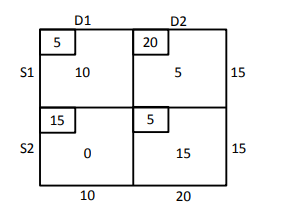
\includegraphics[width=0.75\columnwidth]{chapters/10/7/2/4/figs/fig.png}
 \end{center}
\caption{}
\label{fig:10/7/2/4Fig1}
\end{figure}
\fi

\item Find the position vector of the mid point of the vector joining the points $\vec{P}$(2, 3, 4)
and $\vec{Q}$(4, 1, –2).
\\
\solution
		\begin{enumerate}[label=\thesubsection.\arabic*,ref=\thesubsection.\theenumi]
\item Find the coordinates of the point which divides the join of $(-1,7) $ and $ (4,-3)$ in the ratio 2:3.
	\\
		\solution
	\input{chapters/10/7/2/1/section.tex}
\item Find the coordinates of the point $\vec{R}$ on the line segment joining the points $\vec{P}(-1,3)$ and $\vec{Q}(2,5)$ such that $PR=\frac{3}{5}PQ$.
\item Find the ratio in which the point $\vec{P}\brak{\frac{3}{4},\frac{5}{12}}$ divides the line segment joining the points $\vec{A}\brak{\frac{1}{2},\frac{3}{2}}$ and $ \vec{B}(2,-5)$.
\item Find the coordinates of the point which divides the line segment joining the points $(4,-3)$ and $(8,5)$ in the ratio $3:1$ internally.
\item Find the coordinates of the point $\vec{P}$ on $AD$ such that $AP : PD = 2 : 1$.
\item If the point $\vec{P} (2, 1)$ lies on the line segment joining points $\vec{A} (4, 2)$  and $ \vec{B} (8, 4)$,
then
\begin{enumerate}
	\item $AP =\frac{1}{3}{AB}$ 
\item ${AP}={PE}$
\item ${PB}=\frac{1}{3}{AB}$
\item${AP}=\frac{1}{2}{AB}$
 \end{enumerate}
\item Find the ratio in which the line segment joining the points $(-3,10)$  and  $(6,-8)$  is divided by $ (-1,6)$.
	\\
		\solution
	\input{chapters/10/7/2/4/section.tex}
\item Find the position vector of the mid point of the vector joining the points $\vec{P}$(2, 3, 4)
and $\vec{Q}$(4, 1, –2).
\\
\solution
		\input{chapters/12/10/2/16/section.tex}
\item Let $\vec{A}(4, 2), \vec{B}(6, 5)$  and $ \vec{C}(1, 4)$ be the vertices of $\triangle ABC$.
\begin{enumerate}
\item If $\vec{A}$ and  $\vec{B}$ are $(-2,-2)$ and  $(2,-4)$, respectively, find the coordinates of $\vec{P}$ such that $AP= \frac {3}{7}AB$  and $ \vec{P}$ lies on the line segment $AB$.
	\\
		\solution
	\input{chapters/10/7/2/8/section.tex}
\item Find the coordinates of the points which divide the line segment joining $A(-2,2)$  and  $\vec{B}(2,8)$ into four equal parts.
	\\
		\solution
	\input{chapters/10/7/2/9/section.tex}
\item In what ratio does the point $(-4,6)$ divide the line segment joining the points $\vec{A}(-6,0)$ and $\vec{B}(3,-8)$?
\item Given that $\vec{P}(3,2,-4), \vec{Q}(5,4,-6)$ and $\vec{R}(9,8,-10)$ are collinear. Find the ratio in which $\vec{Q}$ divides $PR$.
\item Points $\vec{A}(-6,10),\vec{B}(-4,6)$  and  $\vec{C}(3,-8)$ are collinear such that $AB=  \frac{2}{9}AC$.
\item The point which divides the line segment joining the points $\vec{P} (7, –6) $  and  $\vec{Q}(3, 4)$ in the 
ratio 1 : 2 internally lies in  which quadrant?
\item Find the coordinates of the points of trisection of the line segment joining $(4,-1)$  and  $(-2,3)$.
	\\
		\solution
	\input{chapters/10/7/2/2/section.tex}
\item Find the coordinates of the points which trisect the line segment joining the points $\vec{P}(4,2,-6)$ and $\vec{Q}(10,-16,6)$.
\item Find the coordinates of the points of trisection (i.e. points dividing to three equal parts) of the line segment joining the points $\vec{A}(2,-2)$ and $\vec{B}(-7,4)$.
\item Point $\vec{P}(5,-3)$ is one of the two points of trisection of line segment joining the points $\vec{A}(7,-2)$ and $\vec{B}(1,-5)$
\item Find the position vector of a point $\vec{R}$ which divides the line joining two points $\vec{P}$
and $\vec{Q}$ whose position vectors are $\hat{i}+2\hat{j}-\hat{k}$ and $-\hat{i}+\hat{j}+\hat{k}$ respectively, in the
ratio 2 : 1
\begin{enumerate}
    \item  internally
    \item  externally
\end{enumerate}
%\solution
%		\input{chapters/12/10/2/15/section.tex}
\item Find the coordinates of the point which divides the line segment joining the points which divides the line segment joining  the points $(-2,3,5)$ and $(1,-4,6)$ in the ratio 
\begin{enumerate}
\item $2:3$ internally,
\item $2:3$ externally
\end{enumerate}
\item Find the coordinates of the point which divides the line segment joining the points $(1,-2,3)$ and $(3,4,-5)$ in the ratio $2:3$
\begin{enumerate}
\item internally, and
\item externally
\end{enumerate}
\item Consider two points $\vec{P}$ and $\vec{Q}$ with position vectors $\overrightarrow{OP} = 3\overrightarrow{a}-2\overrightarrow{b}$ and $\overrightarrow{OQ}=\overrightarrow{a}+\overrightarrow{b}$. Find the position vector of a point $\vec{R}$ which divides the line joining $\vec{P}$ and $\vec{Q}$ in the ratio $2:1$, 
\begin{enumerate}
\item internally, and 
\item externally.
\end{enumerate}
\item The median from $\vec{A}$ meets $BC$ at $\vec{D}$. Find the coordinates of the point $\vec{D}$.
\item Find the coordinates of points $\vec{Q}$ and $\vec{R}$ on medians $BE$ and $CF$ respectively such that $BQ : QE = 2 : 1$  and  $CR : RF = 2 : 1$.
\item What do you observe?
\item If $\vec{A}, \vec{B}$ and $\vec{C}$  are the vertices of $\triangle ABC$, find the coordinates of the centroid of the triangle.
\end{enumerate}
\solution
	\input{chapters/10/7/4/7/section.tex}
\item If $\vec{P}(9a-2,-b)$ divides line segment joining $\vec{A}(3a+1,-3)$ and $\vec{B}(8a,5)$ in the ratio 3:1, find the values of $a$ and $b$.
\item Find the position vector of a point $\vec{R}$ which divides the line joining two points $\vec{P}$ and $\vec{Q}$ whose position vectors are $2\vec{a}+\vec{b}$ and $\vec{a}-3\vec{b}$ externally in the ratio $1:2$.
\item The position vector of the point which divides the join of points 2$\vec{a}$-3$\vec{b}$ $\text{and}$ $\vec{a}+\vec{b}$ in the ratio 3:1 is \rule{1cm}{0.1pt}.
\item If $\vec{a}$ and $\vec{b}$ are the postion vectors of $\vec{A}$ and $\vec{B}$, respectively, find the position vector of a point $\vec{C}$ in $BA$ produced such that $BC=1.5BA$.
\item Find the position vector of a point $\vec{R}$ which divides the line joining two points $\vec{P}$ and $\vec{Q}$ whose position vectors are $(2\vec{a}+\vec{b})$ and $(\vec{a}-3\vec{b})$
externally in the ratio 1 : 2. Also, show that $\vec{P}$ is the mid point of the line segment $RQ$.
\end{enumerate}

\item Let $\vec{A}(4, 2), \vec{B}(6, 5)$  and $ \vec{C}(1, 4)$ be the vertices of $\triangle ABC$.
\begin{enumerate}
\item If $\vec{A}$ and  $\vec{B}$ are $(-2,-2)$ and  $(2,-4)$, respectively, find the coordinates of $\vec{P}$ such that $AP= \frac {3}{7}AB$  and $ \vec{P}$ lies on the line segment $AB$.
	\\
		\solution
	\begin{enumerate}[label=\thesubsection.\arabic*,ref=\thesubsection.\theenumi]
\item Find the coordinates of the point which divides the join of $(-1,7) $ and $ (4,-3)$ in the ratio 2:3.
	\\
		\solution
	\input{chapters/10/7/2/1/section.tex}
\item Find the coordinates of the point $\vec{R}$ on the line segment joining the points $\vec{P}(-1,3)$ and $\vec{Q}(2,5)$ such that $PR=\frac{3}{5}PQ$.
\item Find the ratio in which the point $\vec{P}\brak{\frac{3}{4},\frac{5}{12}}$ divides the line segment joining the points $\vec{A}\brak{\frac{1}{2},\frac{3}{2}}$ and $ \vec{B}(2,-5)$.
\item Find the coordinates of the point which divides the line segment joining the points $(4,-3)$ and $(8,5)$ in the ratio $3:1$ internally.
\item Find the coordinates of the point $\vec{P}$ on $AD$ such that $AP : PD = 2 : 1$.
\item If the point $\vec{P} (2, 1)$ lies on the line segment joining points $\vec{A} (4, 2)$  and $ \vec{B} (8, 4)$,
then
\begin{enumerate}
	\item $AP =\frac{1}{3}{AB}$ 
\item ${AP}={PE}$
\item ${PB}=\frac{1}{3}{AB}$
\item${AP}=\frac{1}{2}{AB}$
 \end{enumerate}
\item Find the ratio in which the line segment joining the points $(-3,10)$  and  $(6,-8)$  is divided by $ (-1,6)$.
	\\
		\solution
	\input{chapters/10/7/2/4/section.tex}
\item Find the position vector of the mid point of the vector joining the points $\vec{P}$(2, 3, 4)
and $\vec{Q}$(4, 1, –2).
\\
\solution
		\input{chapters/12/10/2/16/section.tex}
\item Let $\vec{A}(4, 2), \vec{B}(6, 5)$  and $ \vec{C}(1, 4)$ be the vertices of $\triangle ABC$.
\begin{enumerate}
\item If $\vec{A}$ and  $\vec{B}$ are $(-2,-2)$ and  $(2,-4)$, respectively, find the coordinates of $\vec{P}$ such that $AP= \frac {3}{7}AB$  and $ \vec{P}$ lies on the line segment $AB$.
	\\
		\solution
	\input{chapters/10/7/2/8/section.tex}
\item Find the coordinates of the points which divide the line segment joining $A(-2,2)$  and  $\vec{B}(2,8)$ into four equal parts.
	\\
		\solution
	\input{chapters/10/7/2/9/section.tex}
\item In what ratio does the point $(-4,6)$ divide the line segment joining the points $\vec{A}(-6,0)$ and $\vec{B}(3,-8)$?
\item Given that $\vec{P}(3,2,-4), \vec{Q}(5,4,-6)$ and $\vec{R}(9,8,-10)$ are collinear. Find the ratio in which $\vec{Q}$ divides $PR$.
\item Points $\vec{A}(-6,10),\vec{B}(-4,6)$  and  $\vec{C}(3,-8)$ are collinear such that $AB=  \frac{2}{9}AC$.
\item The point which divides the line segment joining the points $\vec{P} (7, –6) $  and  $\vec{Q}(3, 4)$ in the 
ratio 1 : 2 internally lies in  which quadrant?
\item Find the coordinates of the points of trisection of the line segment joining $(4,-1)$  and  $(-2,3)$.
	\\
		\solution
	\input{chapters/10/7/2/2/section.tex}
\item Find the coordinates of the points which trisect the line segment joining the points $\vec{P}(4,2,-6)$ and $\vec{Q}(10,-16,6)$.
\item Find the coordinates of the points of trisection (i.e. points dividing to three equal parts) of the line segment joining the points $\vec{A}(2,-2)$ and $\vec{B}(-7,4)$.
\item Point $\vec{P}(5,-3)$ is one of the two points of trisection of line segment joining the points $\vec{A}(7,-2)$ and $\vec{B}(1,-5)$
\item Find the position vector of a point $\vec{R}$ which divides the line joining two points $\vec{P}$
and $\vec{Q}$ whose position vectors are $\hat{i}+2\hat{j}-\hat{k}$ and $-\hat{i}+\hat{j}+\hat{k}$ respectively, in the
ratio 2 : 1
\begin{enumerate}
    \item  internally
    \item  externally
\end{enumerate}
%\solution
%		\input{chapters/12/10/2/15/section.tex}
\item Find the coordinates of the point which divides the line segment joining the points which divides the line segment joining  the points $(-2,3,5)$ and $(1,-4,6)$ in the ratio 
\begin{enumerate}
\item $2:3$ internally,
\item $2:3$ externally
\end{enumerate}
\item Find the coordinates of the point which divides the line segment joining the points $(1,-2,3)$ and $(3,4,-5)$ in the ratio $2:3$
\begin{enumerate}
\item internally, and
\item externally
\end{enumerate}
\item Consider two points $\vec{P}$ and $\vec{Q}$ with position vectors $\overrightarrow{OP} = 3\overrightarrow{a}-2\overrightarrow{b}$ and $\overrightarrow{OQ}=\overrightarrow{a}+\overrightarrow{b}$. Find the position vector of a point $\vec{R}$ which divides the line joining $\vec{P}$ and $\vec{Q}$ in the ratio $2:1$, 
\begin{enumerate}
\item internally, and 
\item externally.
\end{enumerate}
\item The median from $\vec{A}$ meets $BC$ at $\vec{D}$. Find the coordinates of the point $\vec{D}$.
\item Find the coordinates of points $\vec{Q}$ and $\vec{R}$ on medians $BE$ and $CF$ respectively such that $BQ : QE = 2 : 1$  and  $CR : RF = 2 : 1$.
\item What do you observe?
\item If $\vec{A}, \vec{B}$ and $\vec{C}$  are the vertices of $\triangle ABC$, find the coordinates of the centroid of the triangle.
\end{enumerate}
\solution
	\input{chapters/10/7/4/7/section.tex}
\item If $\vec{P}(9a-2,-b)$ divides line segment joining $\vec{A}(3a+1,-3)$ and $\vec{B}(8a,5)$ in the ratio 3:1, find the values of $a$ and $b$.
\item Find the position vector of a point $\vec{R}$ which divides the line joining two points $\vec{P}$ and $\vec{Q}$ whose position vectors are $2\vec{a}+\vec{b}$ and $\vec{a}-3\vec{b}$ externally in the ratio $1:2$.
\item The position vector of the point which divides the join of points 2$\vec{a}$-3$\vec{b}$ $\text{and}$ $\vec{a}+\vec{b}$ in the ratio 3:1 is \rule{1cm}{0.1pt}.
\item If $\vec{a}$ and $\vec{b}$ are the postion vectors of $\vec{A}$ and $\vec{B}$, respectively, find the position vector of a point $\vec{C}$ in $BA$ produced such that $BC=1.5BA$.
\item Find the position vector of a point $\vec{R}$ which divides the line joining two points $\vec{P}$ and $\vec{Q}$ whose position vectors are $(2\vec{a}+\vec{b})$ and $(\vec{a}-3\vec{b})$
externally in the ratio 1 : 2. Also, show that $\vec{P}$ is the mid point of the line segment $RQ$.
\end{enumerate}

\item Find the coordinates of the points which divide the line segment joining $A(-2,2)$  and  $\vec{B}(2,8)$ into four equal parts.
	\\
		\solution
	\begin{enumerate}[label=\thesubsection.\arabic*,ref=\thesubsection.\theenumi]
\item Find the coordinates of the point which divides the join of $(-1,7) $ and $ (4,-3)$ in the ratio 2:3.
	\\
		\solution
	\input{chapters/10/7/2/1/section.tex}
\item Find the coordinates of the point $\vec{R}$ on the line segment joining the points $\vec{P}(-1,3)$ and $\vec{Q}(2,5)$ such that $PR=\frac{3}{5}PQ$.
\item Find the ratio in which the point $\vec{P}\brak{\frac{3}{4},\frac{5}{12}}$ divides the line segment joining the points $\vec{A}\brak{\frac{1}{2},\frac{3}{2}}$ and $ \vec{B}(2,-5)$.
\item Find the coordinates of the point which divides the line segment joining the points $(4,-3)$ and $(8,5)$ in the ratio $3:1$ internally.
\item Find the coordinates of the point $\vec{P}$ on $AD$ such that $AP : PD = 2 : 1$.
\item If the point $\vec{P} (2, 1)$ lies on the line segment joining points $\vec{A} (4, 2)$  and $ \vec{B} (8, 4)$,
then
\begin{enumerate}
	\item $AP =\frac{1}{3}{AB}$ 
\item ${AP}={PE}$
\item ${PB}=\frac{1}{3}{AB}$
\item${AP}=\frac{1}{2}{AB}$
 \end{enumerate}
\item Find the ratio in which the line segment joining the points $(-3,10)$  and  $(6,-8)$  is divided by $ (-1,6)$.
	\\
		\solution
	\input{chapters/10/7/2/4/section.tex}
\item Find the position vector of the mid point of the vector joining the points $\vec{P}$(2, 3, 4)
and $\vec{Q}$(4, 1, –2).
\\
\solution
		\input{chapters/12/10/2/16/section.tex}
\item Let $\vec{A}(4, 2), \vec{B}(6, 5)$  and $ \vec{C}(1, 4)$ be the vertices of $\triangle ABC$.
\begin{enumerate}
\item If $\vec{A}$ and  $\vec{B}$ are $(-2,-2)$ and  $(2,-4)$, respectively, find the coordinates of $\vec{P}$ such that $AP= \frac {3}{7}AB$  and $ \vec{P}$ lies on the line segment $AB$.
	\\
		\solution
	\input{chapters/10/7/2/8/section.tex}
\item Find the coordinates of the points which divide the line segment joining $A(-2,2)$  and  $\vec{B}(2,8)$ into four equal parts.
	\\
		\solution
	\input{chapters/10/7/2/9/section.tex}
\item In what ratio does the point $(-4,6)$ divide the line segment joining the points $\vec{A}(-6,0)$ and $\vec{B}(3,-8)$?
\item Given that $\vec{P}(3,2,-4), \vec{Q}(5,4,-6)$ and $\vec{R}(9,8,-10)$ are collinear. Find the ratio in which $\vec{Q}$ divides $PR$.
\item Points $\vec{A}(-6,10),\vec{B}(-4,6)$  and  $\vec{C}(3,-8)$ are collinear such that $AB=  \frac{2}{9}AC$.
\item The point which divides the line segment joining the points $\vec{P} (7, –6) $  and  $\vec{Q}(3, 4)$ in the 
ratio 1 : 2 internally lies in  which quadrant?
\item Find the coordinates of the points of trisection of the line segment joining $(4,-1)$  and  $(-2,3)$.
	\\
		\solution
	\input{chapters/10/7/2/2/section.tex}
\item Find the coordinates of the points which trisect the line segment joining the points $\vec{P}(4,2,-6)$ and $\vec{Q}(10,-16,6)$.
\item Find the coordinates of the points of trisection (i.e. points dividing to three equal parts) of the line segment joining the points $\vec{A}(2,-2)$ and $\vec{B}(-7,4)$.
\item Point $\vec{P}(5,-3)$ is one of the two points of trisection of line segment joining the points $\vec{A}(7,-2)$ and $\vec{B}(1,-5)$
\item Find the position vector of a point $\vec{R}$ which divides the line joining two points $\vec{P}$
and $\vec{Q}$ whose position vectors are $\hat{i}+2\hat{j}-\hat{k}$ and $-\hat{i}+\hat{j}+\hat{k}$ respectively, in the
ratio 2 : 1
\begin{enumerate}
    \item  internally
    \item  externally
\end{enumerate}
%\solution
%		\input{chapters/12/10/2/15/section.tex}
\item Find the coordinates of the point which divides the line segment joining the points which divides the line segment joining  the points $(-2,3,5)$ and $(1,-4,6)$ in the ratio 
\begin{enumerate}
\item $2:3$ internally,
\item $2:3$ externally
\end{enumerate}
\item Find the coordinates of the point which divides the line segment joining the points $(1,-2,3)$ and $(3,4,-5)$ in the ratio $2:3$
\begin{enumerate}
\item internally, and
\item externally
\end{enumerate}
\item Consider two points $\vec{P}$ and $\vec{Q}$ with position vectors $\overrightarrow{OP} = 3\overrightarrow{a}-2\overrightarrow{b}$ and $\overrightarrow{OQ}=\overrightarrow{a}+\overrightarrow{b}$. Find the position vector of a point $\vec{R}$ which divides the line joining $\vec{P}$ and $\vec{Q}$ in the ratio $2:1$, 
\begin{enumerate}
\item internally, and 
\item externally.
\end{enumerate}
\item The median from $\vec{A}$ meets $BC$ at $\vec{D}$. Find the coordinates of the point $\vec{D}$.
\item Find the coordinates of points $\vec{Q}$ and $\vec{R}$ on medians $BE$ and $CF$ respectively such that $BQ : QE = 2 : 1$  and  $CR : RF = 2 : 1$.
\item What do you observe?
\item If $\vec{A}, \vec{B}$ and $\vec{C}$  are the vertices of $\triangle ABC$, find the coordinates of the centroid of the triangle.
\end{enumerate}
\solution
	\input{chapters/10/7/4/7/section.tex}
\item If $\vec{P}(9a-2,-b)$ divides line segment joining $\vec{A}(3a+1,-3)$ and $\vec{B}(8a,5)$ in the ratio 3:1, find the values of $a$ and $b$.
\item Find the position vector of a point $\vec{R}$ which divides the line joining two points $\vec{P}$ and $\vec{Q}$ whose position vectors are $2\vec{a}+\vec{b}$ and $\vec{a}-3\vec{b}$ externally in the ratio $1:2$.
\item The position vector of the point which divides the join of points 2$\vec{a}$-3$\vec{b}$ $\text{and}$ $\vec{a}+\vec{b}$ in the ratio 3:1 is \rule{1cm}{0.1pt}.
\item If $\vec{a}$ and $\vec{b}$ are the postion vectors of $\vec{A}$ and $\vec{B}$, respectively, find the position vector of a point $\vec{C}$ in $BA$ produced such that $BC=1.5BA$.
\item Find the position vector of a point $\vec{R}$ which divides the line joining two points $\vec{P}$ and $\vec{Q}$ whose position vectors are $(2\vec{a}+\vec{b})$ and $(\vec{a}-3\vec{b})$
externally in the ratio 1 : 2. Also, show that $\vec{P}$ is the mid point of the line segment $RQ$.
\end{enumerate}

\item In what ratio does the point $(-4,6)$ divide the line segment joining the points $\vec{A}(-6,0)$ and $\vec{B}(3,-8)$?
\item Given that $\vec{P}(3,2,-4), \vec{Q}(5,4,-6)$ and $\vec{R}(9,8,-10)$ are collinear. Find the ratio in which $\vec{Q}$ divides $PR$.
\item Points $\vec{A}(-6,10),\vec{B}(-4,6)$  and  $\vec{C}(3,-8)$ are collinear such that $AB=  \frac{2}{9}AC$.
\item The point which divides the line segment joining the points $\vec{P} (7, –6) $  and  $\vec{Q}(3, 4)$ in the 
ratio 1 : 2 internally lies in  which quadrant?
\item Find the coordinates of the points of trisection of the line segment joining $(4,-1)$  and  $(-2,3)$.
	\\
		\solution
	Using section formula,
\begin{align}
\vec{R}=\frac{1}{1+\frac{1}{2}}\brak{\myvec{4\\-1}+\frac{1}{2}\myvec{-2\\3}}
=\myvec{2\\ \frac{1}{3}}\\
\vec{S}=\frac{1}{1+\frac{2}{1}}\brak{\myvec{4\\-1}+\frac{2}{1}\myvec{-2\\3}}
=\myvec{0\\ \frac{5}{3}}
\end{align}
which are the desired points of trisection.
\iffalse
See
		\figref{fig:chapters/10/7/2/2/Figure}
\begin{figure}[H]
\centering
\includegraphics[width=0.75\columnwidth]{chapters/10/7/2/2/figs/dj.pdf}
\caption{}
		\label{fig:chapters/10/7/2/2/Figure}
\end{figure}
\fi

\item Find the coordinates of the points which trisect the line segment joining the points $\vec{P}(4,2,-6)$ and $\vec{Q}(10,-16,6)$.
\item Find the coordinates of the points of trisection (i.e. points dividing to three equal parts) of the line segment joining the points $\vec{A}(2,-2)$ and $\vec{B}(-7,4)$.
\item Point $\vec{P}(5,-3)$ is one of the two points of trisection of line segment joining the points $\vec{A}(7,-2)$ and $\vec{B}(1,-5)$
\item Find the position vector of a point $\vec{R}$ which divides the line joining two points $\vec{P}$
and $\vec{Q}$ whose position vectors are $\hat{i}+2\hat{j}-\hat{k}$ and $-\hat{i}+\hat{j}+\hat{k}$ respectively, in the
ratio 2 : 1
\begin{enumerate}
    \item  internally
    \item  externally
\end{enumerate}
%\solution
%		\begin{enumerate}[label=\thesubsection.\arabic*,ref=\thesubsection.\theenumi]
\item Find the coordinates of the point which divides the join of $(-1,7) $ and $ (4,-3)$ in the ratio 2:3.
	\\
		\solution
	\input{chapters/10/7/2/1/section.tex}
\item Find the coordinates of the point $\vec{R}$ on the line segment joining the points $\vec{P}(-1,3)$ and $\vec{Q}(2,5)$ such that $PR=\frac{3}{5}PQ$.
\item Find the ratio in which the point $\vec{P}\brak{\frac{3}{4},\frac{5}{12}}$ divides the line segment joining the points $\vec{A}\brak{\frac{1}{2},\frac{3}{2}}$ and $ \vec{B}(2,-5)$.
\item Find the coordinates of the point which divides the line segment joining the points $(4,-3)$ and $(8,5)$ in the ratio $3:1$ internally.
\item Find the coordinates of the point $\vec{P}$ on $AD$ such that $AP : PD = 2 : 1$.
\item If the point $\vec{P} (2, 1)$ lies on the line segment joining points $\vec{A} (4, 2)$  and $ \vec{B} (8, 4)$,
then
\begin{enumerate}
	\item $AP =\frac{1}{3}{AB}$ 
\item ${AP}={PE}$
\item ${PB}=\frac{1}{3}{AB}$
\item${AP}=\frac{1}{2}{AB}$
 \end{enumerate}
\item Find the ratio in which the line segment joining the points $(-3,10)$  and  $(6,-8)$  is divided by $ (-1,6)$.
	\\
		\solution
	\input{chapters/10/7/2/4/section.tex}
\item Find the position vector of the mid point of the vector joining the points $\vec{P}$(2, 3, 4)
and $\vec{Q}$(4, 1, –2).
\\
\solution
		\input{chapters/12/10/2/16/section.tex}
\item Let $\vec{A}(4, 2), \vec{B}(6, 5)$  and $ \vec{C}(1, 4)$ be the vertices of $\triangle ABC$.
\begin{enumerate}
\item If $\vec{A}$ and  $\vec{B}$ are $(-2,-2)$ and  $(2,-4)$, respectively, find the coordinates of $\vec{P}$ such that $AP= \frac {3}{7}AB$  and $ \vec{P}$ lies on the line segment $AB$.
	\\
		\solution
	\input{chapters/10/7/2/8/section.tex}
\item Find the coordinates of the points which divide the line segment joining $A(-2,2)$  and  $\vec{B}(2,8)$ into four equal parts.
	\\
		\solution
	\input{chapters/10/7/2/9/section.tex}
\item In what ratio does the point $(-4,6)$ divide the line segment joining the points $\vec{A}(-6,0)$ and $\vec{B}(3,-8)$?
\item Given that $\vec{P}(3,2,-4), \vec{Q}(5,4,-6)$ and $\vec{R}(9,8,-10)$ are collinear. Find the ratio in which $\vec{Q}$ divides $PR$.
\item Points $\vec{A}(-6,10),\vec{B}(-4,6)$  and  $\vec{C}(3,-8)$ are collinear such that $AB=  \frac{2}{9}AC$.
\item The point which divides the line segment joining the points $\vec{P} (7, –6) $  and  $\vec{Q}(3, 4)$ in the 
ratio 1 : 2 internally lies in  which quadrant?
\item Find the coordinates of the points of trisection of the line segment joining $(4,-1)$  and  $(-2,3)$.
	\\
		\solution
	\input{chapters/10/7/2/2/section.tex}
\item Find the coordinates of the points which trisect the line segment joining the points $\vec{P}(4,2,-6)$ and $\vec{Q}(10,-16,6)$.
\item Find the coordinates of the points of trisection (i.e. points dividing to three equal parts) of the line segment joining the points $\vec{A}(2,-2)$ and $\vec{B}(-7,4)$.
\item Point $\vec{P}(5,-3)$ is one of the two points of trisection of line segment joining the points $\vec{A}(7,-2)$ and $\vec{B}(1,-5)$
\item Find the position vector of a point $\vec{R}$ which divides the line joining two points $\vec{P}$
and $\vec{Q}$ whose position vectors are $\hat{i}+2\hat{j}-\hat{k}$ and $-\hat{i}+\hat{j}+\hat{k}$ respectively, in the
ratio 2 : 1
\begin{enumerate}
    \item  internally
    \item  externally
\end{enumerate}
%\solution
%		\input{chapters/12/10/2/15/section.tex}
\item Find the coordinates of the point which divides the line segment joining the points which divides the line segment joining  the points $(-2,3,5)$ and $(1,-4,6)$ in the ratio 
\begin{enumerate}
\item $2:3$ internally,
\item $2:3$ externally
\end{enumerate}
\item Find the coordinates of the point which divides the line segment joining the points $(1,-2,3)$ and $(3,4,-5)$ in the ratio $2:3$
\begin{enumerate}
\item internally, and
\item externally
\end{enumerate}
\item Consider two points $\vec{P}$ and $\vec{Q}$ with position vectors $\overrightarrow{OP} = 3\overrightarrow{a}-2\overrightarrow{b}$ and $\overrightarrow{OQ}=\overrightarrow{a}+\overrightarrow{b}$. Find the position vector of a point $\vec{R}$ which divides the line joining $\vec{P}$ and $\vec{Q}$ in the ratio $2:1$, 
\begin{enumerate}
\item internally, and 
\item externally.
\end{enumerate}
\item The median from $\vec{A}$ meets $BC$ at $\vec{D}$. Find the coordinates of the point $\vec{D}$.
\item Find the coordinates of points $\vec{Q}$ and $\vec{R}$ on medians $BE$ and $CF$ respectively such that $BQ : QE = 2 : 1$  and  $CR : RF = 2 : 1$.
\item What do you observe?
\item If $\vec{A}, \vec{B}$ and $\vec{C}$  are the vertices of $\triangle ABC$, find the coordinates of the centroid of the triangle.
\end{enumerate}
\solution
	\input{chapters/10/7/4/7/section.tex}
\item If $\vec{P}(9a-2,-b)$ divides line segment joining $\vec{A}(3a+1,-3)$ and $\vec{B}(8a,5)$ in the ratio 3:1, find the values of $a$ and $b$.
\item Find the position vector of a point $\vec{R}$ which divides the line joining two points $\vec{P}$ and $\vec{Q}$ whose position vectors are $2\vec{a}+\vec{b}$ and $\vec{a}-3\vec{b}$ externally in the ratio $1:2$.
\item The position vector of the point which divides the join of points 2$\vec{a}$-3$\vec{b}$ $\text{and}$ $\vec{a}+\vec{b}$ in the ratio 3:1 is \rule{1cm}{0.1pt}.
\item If $\vec{a}$ and $\vec{b}$ are the postion vectors of $\vec{A}$ and $\vec{B}$, respectively, find the position vector of a point $\vec{C}$ in $BA$ produced such that $BC=1.5BA$.
\item Find the position vector of a point $\vec{R}$ which divides the line joining two points $\vec{P}$ and $\vec{Q}$ whose position vectors are $(2\vec{a}+\vec{b})$ and $(\vec{a}-3\vec{b})$
externally in the ratio 1 : 2. Also, show that $\vec{P}$ is the mid point of the line segment $RQ$.
\end{enumerate}

\item Find the coordinates of the point which divides the line segment joining the points which divides the line segment joining  the points $(-2,3,5)$ and $(1,-4,6)$ in the ratio 
\begin{enumerate}
\item $2:3$ internally,
\item $2:3$ externally
\end{enumerate}
\item Find the coordinates of the point which divides the line segment joining the points $(1,-2,3)$ and $(3,4,-5)$ in the ratio $2:3$
\begin{enumerate}
\item internally, and
\item externally
\end{enumerate}
\item Consider two points $\vec{P}$ and $\vec{Q}$ with position vectors $\overrightarrow{OP} = 3\overrightarrow{a}-2\overrightarrow{b}$ and $\overrightarrow{OQ}=\overrightarrow{a}+\overrightarrow{b}$. Find the position vector of a point $\vec{R}$ which divides the line joining $\vec{P}$ and $\vec{Q}$ in the ratio $2:1$, 
\begin{enumerate}
\item internally, and 
\item externally.
\end{enumerate}
\item The median from $\vec{A}$ meets $BC$ at $\vec{D}$. Find the coordinates of the point $\vec{D}$.
\item Find the coordinates of points $\vec{Q}$ and $\vec{R}$ on medians $BE$ and $CF$ respectively such that $BQ : QE = 2 : 1$  and  $CR : RF = 2 : 1$.
\item What do you observe?
\item If $\vec{A}, \vec{B}$ and $\vec{C}$  are the vertices of $\triangle ABC$, find the coordinates of the centroid of the triangle.
\end{enumerate}
\solution
	\begin{enumerate}[label=\thesubsection.\arabic*,ref=\thesubsection.\theenumi]
\item Find the coordinates of the point which divides the join of $(-1,7) $ and $ (4,-3)$ in the ratio 2:3.
	\\
		\solution
	\input{chapters/10/7/2/1/section.tex}
\item Find the coordinates of the point $\vec{R}$ on the line segment joining the points $\vec{P}(-1,3)$ and $\vec{Q}(2,5)$ such that $PR=\frac{3}{5}PQ$.
\item Find the ratio in which the point $\vec{P}\brak{\frac{3}{4},\frac{5}{12}}$ divides the line segment joining the points $\vec{A}\brak{\frac{1}{2},\frac{3}{2}}$ and $ \vec{B}(2,-5)$.
\item Find the coordinates of the point which divides the line segment joining the points $(4,-3)$ and $(8,5)$ in the ratio $3:1$ internally.
\item Find the coordinates of the point $\vec{P}$ on $AD$ such that $AP : PD = 2 : 1$.
\item If the point $\vec{P} (2, 1)$ lies on the line segment joining points $\vec{A} (4, 2)$  and $ \vec{B} (8, 4)$,
then
\begin{enumerate}
	\item $AP =\frac{1}{3}{AB}$ 
\item ${AP}={PE}$
\item ${PB}=\frac{1}{3}{AB}$
\item${AP}=\frac{1}{2}{AB}$
 \end{enumerate}
\item Find the ratio in which the line segment joining the points $(-3,10)$  and  $(6,-8)$  is divided by $ (-1,6)$.
	\\
		\solution
	\input{chapters/10/7/2/4/section.tex}
\item Find the position vector of the mid point of the vector joining the points $\vec{P}$(2, 3, 4)
and $\vec{Q}$(4, 1, –2).
\\
\solution
		\input{chapters/12/10/2/16/section.tex}
\item Let $\vec{A}(4, 2), \vec{B}(6, 5)$  and $ \vec{C}(1, 4)$ be the vertices of $\triangle ABC$.
\begin{enumerate}
\item If $\vec{A}$ and  $\vec{B}$ are $(-2,-2)$ and  $(2,-4)$, respectively, find the coordinates of $\vec{P}$ such that $AP= \frac {3}{7}AB$  and $ \vec{P}$ lies on the line segment $AB$.
	\\
		\solution
	\input{chapters/10/7/2/8/section.tex}
\item Find the coordinates of the points which divide the line segment joining $A(-2,2)$  and  $\vec{B}(2,8)$ into four equal parts.
	\\
		\solution
	\input{chapters/10/7/2/9/section.tex}
\item In what ratio does the point $(-4,6)$ divide the line segment joining the points $\vec{A}(-6,0)$ and $\vec{B}(3,-8)$?
\item Given that $\vec{P}(3,2,-4), \vec{Q}(5,4,-6)$ and $\vec{R}(9,8,-10)$ are collinear. Find the ratio in which $\vec{Q}$ divides $PR$.
\item Points $\vec{A}(-6,10),\vec{B}(-4,6)$  and  $\vec{C}(3,-8)$ are collinear such that $AB=  \frac{2}{9}AC$.
\item The point which divides the line segment joining the points $\vec{P} (7, –6) $  and  $\vec{Q}(3, 4)$ in the 
ratio 1 : 2 internally lies in  which quadrant?
\item Find the coordinates of the points of trisection of the line segment joining $(4,-1)$  and  $(-2,3)$.
	\\
		\solution
	\input{chapters/10/7/2/2/section.tex}
\item Find the coordinates of the points which trisect the line segment joining the points $\vec{P}(4,2,-6)$ and $\vec{Q}(10,-16,6)$.
\item Find the coordinates of the points of trisection (i.e. points dividing to three equal parts) of the line segment joining the points $\vec{A}(2,-2)$ and $\vec{B}(-7,4)$.
\item Point $\vec{P}(5,-3)$ is one of the two points of trisection of line segment joining the points $\vec{A}(7,-2)$ and $\vec{B}(1,-5)$
\item Find the position vector of a point $\vec{R}$ which divides the line joining two points $\vec{P}$
and $\vec{Q}$ whose position vectors are $\hat{i}+2\hat{j}-\hat{k}$ and $-\hat{i}+\hat{j}+\hat{k}$ respectively, in the
ratio 2 : 1
\begin{enumerate}
    \item  internally
    \item  externally
\end{enumerate}
%\solution
%		\input{chapters/12/10/2/15/section.tex}
\item Find the coordinates of the point which divides the line segment joining the points which divides the line segment joining  the points $(-2,3,5)$ and $(1,-4,6)$ in the ratio 
\begin{enumerate}
\item $2:3$ internally,
\item $2:3$ externally
\end{enumerate}
\item Find the coordinates of the point which divides the line segment joining the points $(1,-2,3)$ and $(3,4,-5)$ in the ratio $2:3$
\begin{enumerate}
\item internally, and
\item externally
\end{enumerate}
\item Consider two points $\vec{P}$ and $\vec{Q}$ with position vectors $\overrightarrow{OP} = 3\overrightarrow{a}-2\overrightarrow{b}$ and $\overrightarrow{OQ}=\overrightarrow{a}+\overrightarrow{b}$. Find the position vector of a point $\vec{R}$ which divides the line joining $\vec{P}$ and $\vec{Q}$ in the ratio $2:1$, 
\begin{enumerate}
\item internally, and 
\item externally.
\end{enumerate}
\item The median from $\vec{A}$ meets $BC$ at $\vec{D}$. Find the coordinates of the point $\vec{D}$.
\item Find the coordinates of points $\vec{Q}$ and $\vec{R}$ on medians $BE$ and $CF$ respectively such that $BQ : QE = 2 : 1$  and  $CR : RF = 2 : 1$.
\item What do you observe?
\item If $\vec{A}, \vec{B}$ and $\vec{C}$  are the vertices of $\triangle ABC$, find the coordinates of the centroid of the triangle.
\end{enumerate}
\solution
	\input{chapters/10/7/4/7/section.tex}
\item If $\vec{P}(9a-2,-b)$ divides line segment joining $\vec{A}(3a+1,-3)$ and $\vec{B}(8a,5)$ in the ratio 3:1, find the values of $a$ and $b$.
\item Find the position vector of a point $\vec{R}$ which divides the line joining two points $\vec{P}$ and $\vec{Q}$ whose position vectors are $2\vec{a}+\vec{b}$ and $\vec{a}-3\vec{b}$ externally in the ratio $1:2$.
\item The position vector of the point which divides the join of points 2$\vec{a}$-3$\vec{b}$ $\text{and}$ $\vec{a}+\vec{b}$ in the ratio 3:1 is \rule{1cm}{0.1pt}.
\item If $\vec{a}$ and $\vec{b}$ are the postion vectors of $\vec{A}$ and $\vec{B}$, respectively, find the position vector of a point $\vec{C}$ in $BA$ produced such that $BC=1.5BA$.
\item Find the position vector of a point $\vec{R}$ which divides the line joining two points $\vec{P}$ and $\vec{Q}$ whose position vectors are $(2\vec{a}+\vec{b})$ and $(\vec{a}-3\vec{b})$
externally in the ratio 1 : 2. Also, show that $\vec{P}$ is the mid point of the line segment $RQ$.
\end{enumerate}

\item If $\vec{P}(9a-2,-b)$ divides line segment joining $\vec{A}(3a+1,-3)$ and $\vec{B}(8a,5)$ in the ratio 3:1, find the values of $a$ and $b$.
\item Find the position vector of a point $\vec{R}$ which divides the line joining two points $\vec{P}$ and $\vec{Q}$ whose position vectors are $2\vec{a}+\vec{b}$ and $\vec{a}-3\vec{b}$ externally in the ratio $1:2$.
\item The position vector of the point which divides the join of points 2$\vec{a}$-3$\vec{b}$ $\text{and}$ $\vec{a}+\vec{b}$ in the ratio 3:1 is \rule{1cm}{0.1pt}.
\item If $\vec{a}$ and $\vec{b}$ are the postion vectors of $\vec{A}$ and $\vec{B}$, respectively, find the position vector of a point $\vec{C}$ in $BA$ produced such that $BC=1.5BA$.
\item Find the position vector of a point $\vec{R}$ which divides the line joining two points $\vec{P}$ and $\vec{Q}$ whose position vectors are $(2\vec{a}+\vec{b})$ and $(\vec{a}-3\vec{b})$
externally in the ratio 1 : 2. Also, show that $\vec{P}$ is the mid point of the line segment $RQ$.
\end{enumerate}

\item Find the coordinates of the point which divides the line segment joining the points which divides the line segment joining  the points $(-2,3,5)$ and $(1,-4,6)$ in the ratio 
\begin{enumerate}
\item $2:3$ internally,
\item $2:3$ externally
\end{enumerate}
\item Find the coordinates of the point which divides the line segment joining the points $(1,-2,3)$ and $(3,4,-5)$ in the ratio $2:3$
\begin{enumerate}
\item internally, and
\item externally
\end{enumerate}
\item Consider two points $\vec{P}$ and $\vec{Q}$ with position vectors $\overrightarrow{OP} = 3\overrightarrow{a}-2\overrightarrow{b}$ and $\overrightarrow{OQ}=\overrightarrow{a}+\overrightarrow{b}$. Find the position vector of a point $\vec{R}$ which divides the line joining $\vec{P}$ and $\vec{Q}$ in the ratio $2:1$, 
\begin{enumerate}
\item internally, and 
\item externally.
\end{enumerate}
\item The median from $\vec{A}$ meets $BC$ at $\vec{D}$. Find the coordinates of the point $\vec{D}$.
\item Find the coordinates of points $\vec{Q}$ and $\vec{R}$ on medians $BE$ and $CF$ respectively such that $BQ : QE = 2 : 1$  and  $CR : RF = 2 : 1$.
\item What do you observe?
\item If $\vec{A}, \vec{B}$ and $\vec{C}$  are the vertices of $\triangle ABC$, find the coordinates of the centroid of the triangle.
\end{enumerate}
\solution
	\begin{enumerate}[label=\thesubsection.\arabic*,ref=\thesubsection.\theenumi]
\item Find the coordinates of the point which divides the join of $(-1,7) $ and $ (4,-3)$ in the ratio 2:3.
	\\
		\solution
	\begin{enumerate}[label=\thesubsection.\arabic*,ref=\thesubsection.\theenumi]
\item Find the coordinates of the point which divides the join of $(-1,7) $ and $ (4,-3)$ in the ratio 2:3.
	\\
		\solution
	\input{chapters/10/7/2/1/section.tex}
\item Find the coordinates of the point $\vec{R}$ on the line segment joining the points $\vec{P}(-1,3)$ and $\vec{Q}(2,5)$ such that $PR=\frac{3}{5}PQ$.
\item Find the ratio in which the point $\vec{P}\brak{\frac{3}{4},\frac{5}{12}}$ divides the line segment joining the points $\vec{A}\brak{\frac{1}{2},\frac{3}{2}}$ and $ \vec{B}(2,-5)$.
\item Find the coordinates of the point which divides the line segment joining the points $(4,-3)$ and $(8,5)$ in the ratio $3:1$ internally.
\item Find the coordinates of the point $\vec{P}$ on $AD$ such that $AP : PD = 2 : 1$.
\item If the point $\vec{P} (2, 1)$ lies on the line segment joining points $\vec{A} (4, 2)$  and $ \vec{B} (8, 4)$,
then
\begin{enumerate}
	\item $AP =\frac{1}{3}{AB}$ 
\item ${AP}={PE}$
\item ${PB}=\frac{1}{3}{AB}$
\item${AP}=\frac{1}{2}{AB}$
 \end{enumerate}
\item Find the ratio in which the line segment joining the points $(-3,10)$  and  $(6,-8)$  is divided by $ (-1,6)$.
	\\
		\solution
	\input{chapters/10/7/2/4/section.tex}
\item Find the position vector of the mid point of the vector joining the points $\vec{P}$(2, 3, 4)
and $\vec{Q}$(4, 1, –2).
\\
\solution
		\input{chapters/12/10/2/16/section.tex}
\item Let $\vec{A}(4, 2), \vec{B}(6, 5)$  and $ \vec{C}(1, 4)$ be the vertices of $\triangle ABC$.
\begin{enumerate}
\item If $\vec{A}$ and  $\vec{B}$ are $(-2,-2)$ and  $(2,-4)$, respectively, find the coordinates of $\vec{P}$ such that $AP= \frac {3}{7}AB$  and $ \vec{P}$ lies on the line segment $AB$.
	\\
		\solution
	\input{chapters/10/7/2/8/section.tex}
\item Find the coordinates of the points which divide the line segment joining $A(-2,2)$  and  $\vec{B}(2,8)$ into four equal parts.
	\\
		\solution
	\input{chapters/10/7/2/9/section.tex}
\item In what ratio does the point $(-4,6)$ divide the line segment joining the points $\vec{A}(-6,0)$ and $\vec{B}(3,-8)$?
\item Given that $\vec{P}(3,2,-4), \vec{Q}(5,4,-6)$ and $\vec{R}(9,8,-10)$ are collinear. Find the ratio in which $\vec{Q}$ divides $PR$.
\item Points $\vec{A}(-6,10),\vec{B}(-4,6)$  and  $\vec{C}(3,-8)$ are collinear such that $AB=  \frac{2}{9}AC$.
\item The point which divides the line segment joining the points $\vec{P} (7, –6) $  and  $\vec{Q}(3, 4)$ in the 
ratio 1 : 2 internally lies in  which quadrant?
\item Find the coordinates of the points of trisection of the line segment joining $(4,-1)$  and  $(-2,3)$.
	\\
		\solution
	\input{chapters/10/7/2/2/section.tex}
\item Find the coordinates of the points which trisect the line segment joining the points $\vec{P}(4,2,-6)$ and $\vec{Q}(10,-16,6)$.
\item Find the coordinates of the points of trisection (i.e. points dividing to three equal parts) of the line segment joining the points $\vec{A}(2,-2)$ and $\vec{B}(-7,4)$.
\item Point $\vec{P}(5,-3)$ is one of the two points of trisection of line segment joining the points $\vec{A}(7,-2)$ and $\vec{B}(1,-5)$
\item Find the position vector of a point $\vec{R}$ which divides the line joining two points $\vec{P}$
and $\vec{Q}$ whose position vectors are $\hat{i}+2\hat{j}-\hat{k}$ and $-\hat{i}+\hat{j}+\hat{k}$ respectively, in the
ratio 2 : 1
\begin{enumerate}
    \item  internally
    \item  externally
\end{enumerate}
%\solution
%		\input{chapters/12/10/2/15/section.tex}
\item Find the coordinates of the point which divides the line segment joining the points which divides the line segment joining  the points $(-2,3,5)$ and $(1,-4,6)$ in the ratio 
\begin{enumerate}
\item $2:3$ internally,
\item $2:3$ externally
\end{enumerate}
\item Find the coordinates of the point which divides the line segment joining the points $(1,-2,3)$ and $(3,4,-5)$ in the ratio $2:3$
\begin{enumerate}
\item internally, and
\item externally
\end{enumerate}
\item Consider two points $\vec{P}$ and $\vec{Q}$ with position vectors $\overrightarrow{OP} = 3\overrightarrow{a}-2\overrightarrow{b}$ and $\overrightarrow{OQ}=\overrightarrow{a}+\overrightarrow{b}$. Find the position vector of a point $\vec{R}$ which divides the line joining $\vec{P}$ and $\vec{Q}$ in the ratio $2:1$, 
\begin{enumerate}
\item internally, and 
\item externally.
\end{enumerate}
\item The median from $\vec{A}$ meets $BC$ at $\vec{D}$. Find the coordinates of the point $\vec{D}$.
\item Find the coordinates of points $\vec{Q}$ and $\vec{R}$ on medians $BE$ and $CF$ respectively such that $BQ : QE = 2 : 1$  and  $CR : RF = 2 : 1$.
\item What do you observe?
\item If $\vec{A}, \vec{B}$ and $\vec{C}$  are the vertices of $\triangle ABC$, find the coordinates of the centroid of the triangle.
\end{enumerate}
\solution
	\input{chapters/10/7/4/7/section.tex}
\item If $\vec{P}(9a-2,-b)$ divides line segment joining $\vec{A}(3a+1,-3)$ and $\vec{B}(8a,5)$ in the ratio 3:1, find the values of $a$ and $b$.
\item Find the position vector of a point $\vec{R}$ which divides the line joining two points $\vec{P}$ and $\vec{Q}$ whose position vectors are $2\vec{a}+\vec{b}$ and $\vec{a}-3\vec{b}$ externally in the ratio $1:2$.
\item The position vector of the point which divides the join of points 2$\vec{a}$-3$\vec{b}$ $\text{and}$ $\vec{a}+\vec{b}$ in the ratio 3:1 is \rule{1cm}{0.1pt}.
\item If $\vec{a}$ and $\vec{b}$ are the postion vectors of $\vec{A}$ and $\vec{B}$, respectively, find the position vector of a point $\vec{C}$ in $BA$ produced such that $BC=1.5BA$.
\item Find the position vector of a point $\vec{R}$ which divides the line joining two points $\vec{P}$ and $\vec{Q}$ whose position vectors are $(2\vec{a}+\vec{b})$ and $(\vec{a}-3\vec{b})$
externally in the ratio 1 : 2. Also, show that $\vec{P}$ is the mid point of the line segment $RQ$.
\end{enumerate}

\item Find the coordinates of the point $\vec{R}$ on the line segment joining the points $\vec{P}(-1,3)$ and $\vec{Q}(2,5)$ such that $PR=\frac{3}{5}PQ$.
\item Find the ratio in which the point $\vec{P}\brak{\frac{3}{4},\frac{5}{12}}$ divides the line segment joining the points $\vec{A}\brak{\frac{1}{2},\frac{3}{2}}$ and $ \vec{B}(2,-5)$.
\item Find the coordinates of the point which divides the line segment joining the points $(4,-3)$ and $(8,5)$ in the ratio $3:1$ internally.
\item Find the coordinates of the point $\vec{P}$ on $AD$ such that $AP : PD = 2 : 1$.
\item If the point $\vec{P} (2, 1)$ lies on the line segment joining points $\vec{A} (4, 2)$  and $ \vec{B} (8, 4)$,
then
\begin{enumerate}
	\item $AP =\frac{1}{3}{AB}$ 
\item ${AP}={PE}$
\item ${PB}=\frac{1}{3}{AB}$
\item${AP}=\frac{1}{2}{AB}$
 \end{enumerate}
\item Find the ratio in which the line segment joining the points $(-3,10)$  and  $(6,-8)$  is divided by $ (-1,6)$.
	\\
		\solution
	\iffalse
Using section formula,
\begin{align}
         \myvec{-1\\6} &=\frac{{\myvec{-3\\10}+k\myvec{6\\-8}}}{1+k}\\
	 \implies 7k\myvec{1 \\ -2} &= 2\myvec{1 \\ -2}
	 \\
	 \text{or, } k &= \frac{2}{7}.
\end{align}
\fi
In 
			\eqref{eq:section_formula-k}, substituting
			\begin{align}
				\vec{B} &= \myvec{-3\\10}, \vec{C} = \myvec{6\\-8}, \vec{D} = \myvec{-1\\6},
				\\
				k &= \frac{\myvec{-2 & 4}\myvec{-7 \\ 14}}{\norm{\myvec{-7 \\ 14}}^2} = \frac{2}{7}
			\end{align}
\iffalse
See \figref{fig:10/7/2/4Fig1}.
\begin{figure}[H]
 \begin{center}
  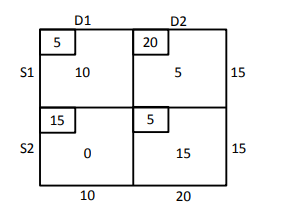
\includegraphics[width=0.75\columnwidth]{chapters/10/7/2/4/figs/fig.png}
 \end{center}
\caption{}
\label{fig:10/7/2/4Fig1}
\end{figure}
\fi

\item Find the position vector of the mid point of the vector joining the points $\vec{P}$(2, 3, 4)
and $\vec{Q}$(4, 1, –2).
\\
\solution
		\begin{enumerate}[label=\thesubsection.\arabic*,ref=\thesubsection.\theenumi]
\item Find the coordinates of the point which divides the join of $(-1,7) $ and $ (4,-3)$ in the ratio 2:3.
	\\
		\solution
	\input{chapters/10/7/2/1/section.tex}
\item Find the coordinates of the point $\vec{R}$ on the line segment joining the points $\vec{P}(-1,3)$ and $\vec{Q}(2,5)$ such that $PR=\frac{3}{5}PQ$.
\item Find the ratio in which the point $\vec{P}\brak{\frac{3}{4},\frac{5}{12}}$ divides the line segment joining the points $\vec{A}\brak{\frac{1}{2},\frac{3}{2}}$ and $ \vec{B}(2,-5)$.
\item Find the coordinates of the point which divides the line segment joining the points $(4,-3)$ and $(8,5)$ in the ratio $3:1$ internally.
\item Find the coordinates of the point $\vec{P}$ on $AD$ such that $AP : PD = 2 : 1$.
\item If the point $\vec{P} (2, 1)$ lies on the line segment joining points $\vec{A} (4, 2)$  and $ \vec{B} (8, 4)$,
then
\begin{enumerate}
	\item $AP =\frac{1}{3}{AB}$ 
\item ${AP}={PE}$
\item ${PB}=\frac{1}{3}{AB}$
\item${AP}=\frac{1}{2}{AB}$
 \end{enumerate}
\item Find the ratio in which the line segment joining the points $(-3,10)$  and  $(6,-8)$  is divided by $ (-1,6)$.
	\\
		\solution
	\input{chapters/10/7/2/4/section.tex}
\item Find the position vector of the mid point of the vector joining the points $\vec{P}$(2, 3, 4)
and $\vec{Q}$(4, 1, –2).
\\
\solution
		\input{chapters/12/10/2/16/section.tex}
\item Let $\vec{A}(4, 2), \vec{B}(6, 5)$  and $ \vec{C}(1, 4)$ be the vertices of $\triangle ABC$.
\begin{enumerate}
\item If $\vec{A}$ and  $\vec{B}$ are $(-2,-2)$ and  $(2,-4)$, respectively, find the coordinates of $\vec{P}$ such that $AP= \frac {3}{7}AB$  and $ \vec{P}$ lies on the line segment $AB$.
	\\
		\solution
	\input{chapters/10/7/2/8/section.tex}
\item Find the coordinates of the points which divide the line segment joining $A(-2,2)$  and  $\vec{B}(2,8)$ into four equal parts.
	\\
		\solution
	\input{chapters/10/7/2/9/section.tex}
\item In what ratio does the point $(-4,6)$ divide the line segment joining the points $\vec{A}(-6,0)$ and $\vec{B}(3,-8)$?
\item Given that $\vec{P}(3,2,-4), \vec{Q}(5,4,-6)$ and $\vec{R}(9,8,-10)$ are collinear. Find the ratio in which $\vec{Q}$ divides $PR$.
\item Points $\vec{A}(-6,10),\vec{B}(-4,6)$  and  $\vec{C}(3,-8)$ are collinear such that $AB=  \frac{2}{9}AC$.
\item The point which divides the line segment joining the points $\vec{P} (7, –6) $  and  $\vec{Q}(3, 4)$ in the 
ratio 1 : 2 internally lies in  which quadrant?
\item Find the coordinates of the points of trisection of the line segment joining $(4,-1)$  and  $(-2,3)$.
	\\
		\solution
	\input{chapters/10/7/2/2/section.tex}
\item Find the coordinates of the points which trisect the line segment joining the points $\vec{P}(4,2,-6)$ and $\vec{Q}(10,-16,6)$.
\item Find the coordinates of the points of trisection (i.e. points dividing to three equal parts) of the line segment joining the points $\vec{A}(2,-2)$ and $\vec{B}(-7,4)$.
\item Point $\vec{P}(5,-3)$ is one of the two points of trisection of line segment joining the points $\vec{A}(7,-2)$ and $\vec{B}(1,-5)$
\item Find the position vector of a point $\vec{R}$ which divides the line joining two points $\vec{P}$
and $\vec{Q}$ whose position vectors are $\hat{i}+2\hat{j}-\hat{k}$ and $-\hat{i}+\hat{j}+\hat{k}$ respectively, in the
ratio 2 : 1
\begin{enumerate}
    \item  internally
    \item  externally
\end{enumerate}
%\solution
%		\input{chapters/12/10/2/15/section.tex}
\item Find the coordinates of the point which divides the line segment joining the points which divides the line segment joining  the points $(-2,3,5)$ and $(1,-4,6)$ in the ratio 
\begin{enumerate}
\item $2:3$ internally,
\item $2:3$ externally
\end{enumerate}
\item Find the coordinates of the point which divides the line segment joining the points $(1,-2,3)$ and $(3,4,-5)$ in the ratio $2:3$
\begin{enumerate}
\item internally, and
\item externally
\end{enumerate}
\item Consider two points $\vec{P}$ and $\vec{Q}$ with position vectors $\overrightarrow{OP} = 3\overrightarrow{a}-2\overrightarrow{b}$ and $\overrightarrow{OQ}=\overrightarrow{a}+\overrightarrow{b}$. Find the position vector of a point $\vec{R}$ which divides the line joining $\vec{P}$ and $\vec{Q}$ in the ratio $2:1$, 
\begin{enumerate}
\item internally, and 
\item externally.
\end{enumerate}
\item The median from $\vec{A}$ meets $BC$ at $\vec{D}$. Find the coordinates of the point $\vec{D}$.
\item Find the coordinates of points $\vec{Q}$ and $\vec{R}$ on medians $BE$ and $CF$ respectively such that $BQ : QE = 2 : 1$  and  $CR : RF = 2 : 1$.
\item What do you observe?
\item If $\vec{A}, \vec{B}$ and $\vec{C}$  are the vertices of $\triangle ABC$, find the coordinates of the centroid of the triangle.
\end{enumerate}
\solution
	\input{chapters/10/7/4/7/section.tex}
\item If $\vec{P}(9a-2,-b)$ divides line segment joining $\vec{A}(3a+1,-3)$ and $\vec{B}(8a,5)$ in the ratio 3:1, find the values of $a$ and $b$.
\item Find the position vector of a point $\vec{R}$ which divides the line joining two points $\vec{P}$ and $\vec{Q}$ whose position vectors are $2\vec{a}+\vec{b}$ and $\vec{a}-3\vec{b}$ externally in the ratio $1:2$.
\item The position vector of the point which divides the join of points 2$\vec{a}$-3$\vec{b}$ $\text{and}$ $\vec{a}+\vec{b}$ in the ratio 3:1 is \rule{1cm}{0.1pt}.
\item If $\vec{a}$ and $\vec{b}$ are the postion vectors of $\vec{A}$ and $\vec{B}$, respectively, find the position vector of a point $\vec{C}$ in $BA$ produced such that $BC=1.5BA$.
\item Find the position vector of a point $\vec{R}$ which divides the line joining two points $\vec{P}$ and $\vec{Q}$ whose position vectors are $(2\vec{a}+\vec{b})$ and $(\vec{a}-3\vec{b})$
externally in the ratio 1 : 2. Also, show that $\vec{P}$ is the mid point of the line segment $RQ$.
\end{enumerate}

\item Let $\vec{A}(4, 2), \vec{B}(6, 5)$  and $ \vec{C}(1, 4)$ be the vertices of $\triangle ABC$.
\begin{enumerate}
\item If $\vec{A}$ and  $\vec{B}$ are $(-2,-2)$ and  $(2,-4)$, respectively, find the coordinates of $\vec{P}$ such that $AP= \frac {3}{7}AB$  and $ \vec{P}$ lies on the line segment $AB$.
	\\
		\solution
	\begin{enumerate}[label=\thesubsection.\arabic*,ref=\thesubsection.\theenumi]
\item Find the coordinates of the point which divides the join of $(-1,7) $ and $ (4,-3)$ in the ratio 2:3.
	\\
		\solution
	\input{chapters/10/7/2/1/section.tex}
\item Find the coordinates of the point $\vec{R}$ on the line segment joining the points $\vec{P}(-1,3)$ and $\vec{Q}(2,5)$ such that $PR=\frac{3}{5}PQ$.
\item Find the ratio in which the point $\vec{P}\brak{\frac{3}{4},\frac{5}{12}}$ divides the line segment joining the points $\vec{A}\brak{\frac{1}{2},\frac{3}{2}}$ and $ \vec{B}(2,-5)$.
\item Find the coordinates of the point which divides the line segment joining the points $(4,-3)$ and $(8,5)$ in the ratio $3:1$ internally.
\item Find the coordinates of the point $\vec{P}$ on $AD$ such that $AP : PD = 2 : 1$.
\item If the point $\vec{P} (2, 1)$ lies on the line segment joining points $\vec{A} (4, 2)$  and $ \vec{B} (8, 4)$,
then
\begin{enumerate}
	\item $AP =\frac{1}{3}{AB}$ 
\item ${AP}={PE}$
\item ${PB}=\frac{1}{3}{AB}$
\item${AP}=\frac{1}{2}{AB}$
 \end{enumerate}
\item Find the ratio in which the line segment joining the points $(-3,10)$  and  $(6,-8)$  is divided by $ (-1,6)$.
	\\
		\solution
	\input{chapters/10/7/2/4/section.tex}
\item Find the position vector of the mid point of the vector joining the points $\vec{P}$(2, 3, 4)
and $\vec{Q}$(4, 1, –2).
\\
\solution
		\input{chapters/12/10/2/16/section.tex}
\item Let $\vec{A}(4, 2), \vec{B}(6, 5)$  and $ \vec{C}(1, 4)$ be the vertices of $\triangle ABC$.
\begin{enumerate}
\item If $\vec{A}$ and  $\vec{B}$ are $(-2,-2)$ and  $(2,-4)$, respectively, find the coordinates of $\vec{P}$ such that $AP= \frac {3}{7}AB$  and $ \vec{P}$ lies on the line segment $AB$.
	\\
		\solution
	\input{chapters/10/7/2/8/section.tex}
\item Find the coordinates of the points which divide the line segment joining $A(-2,2)$  and  $\vec{B}(2,8)$ into four equal parts.
	\\
		\solution
	\input{chapters/10/7/2/9/section.tex}
\item In what ratio does the point $(-4,6)$ divide the line segment joining the points $\vec{A}(-6,0)$ and $\vec{B}(3,-8)$?
\item Given that $\vec{P}(3,2,-4), \vec{Q}(5,4,-6)$ and $\vec{R}(9,8,-10)$ are collinear. Find the ratio in which $\vec{Q}$ divides $PR$.
\item Points $\vec{A}(-6,10),\vec{B}(-4,6)$  and  $\vec{C}(3,-8)$ are collinear such that $AB=  \frac{2}{9}AC$.
\item The point which divides the line segment joining the points $\vec{P} (7, –6) $  and  $\vec{Q}(3, 4)$ in the 
ratio 1 : 2 internally lies in  which quadrant?
\item Find the coordinates of the points of trisection of the line segment joining $(4,-1)$  and  $(-2,3)$.
	\\
		\solution
	\input{chapters/10/7/2/2/section.tex}
\item Find the coordinates of the points which trisect the line segment joining the points $\vec{P}(4,2,-6)$ and $\vec{Q}(10,-16,6)$.
\item Find the coordinates of the points of trisection (i.e. points dividing to three equal parts) of the line segment joining the points $\vec{A}(2,-2)$ and $\vec{B}(-7,4)$.
\item Point $\vec{P}(5,-3)$ is one of the two points of trisection of line segment joining the points $\vec{A}(7,-2)$ and $\vec{B}(1,-5)$
\item Find the position vector of a point $\vec{R}$ which divides the line joining two points $\vec{P}$
and $\vec{Q}$ whose position vectors are $\hat{i}+2\hat{j}-\hat{k}$ and $-\hat{i}+\hat{j}+\hat{k}$ respectively, in the
ratio 2 : 1
\begin{enumerate}
    \item  internally
    \item  externally
\end{enumerate}
%\solution
%		\input{chapters/12/10/2/15/section.tex}
\item Find the coordinates of the point which divides the line segment joining the points which divides the line segment joining  the points $(-2,3,5)$ and $(1,-4,6)$ in the ratio 
\begin{enumerate}
\item $2:3$ internally,
\item $2:3$ externally
\end{enumerate}
\item Find the coordinates of the point which divides the line segment joining the points $(1,-2,3)$ and $(3,4,-5)$ in the ratio $2:3$
\begin{enumerate}
\item internally, and
\item externally
\end{enumerate}
\item Consider two points $\vec{P}$ and $\vec{Q}$ with position vectors $\overrightarrow{OP} = 3\overrightarrow{a}-2\overrightarrow{b}$ and $\overrightarrow{OQ}=\overrightarrow{a}+\overrightarrow{b}$. Find the position vector of a point $\vec{R}$ which divides the line joining $\vec{P}$ and $\vec{Q}$ in the ratio $2:1$, 
\begin{enumerate}
\item internally, and 
\item externally.
\end{enumerate}
\item The median from $\vec{A}$ meets $BC$ at $\vec{D}$. Find the coordinates of the point $\vec{D}$.
\item Find the coordinates of points $\vec{Q}$ and $\vec{R}$ on medians $BE$ and $CF$ respectively such that $BQ : QE = 2 : 1$  and  $CR : RF = 2 : 1$.
\item What do you observe?
\item If $\vec{A}, \vec{B}$ and $\vec{C}$  are the vertices of $\triangle ABC$, find the coordinates of the centroid of the triangle.
\end{enumerate}
\solution
	\input{chapters/10/7/4/7/section.tex}
\item If $\vec{P}(9a-2,-b)$ divides line segment joining $\vec{A}(3a+1,-3)$ and $\vec{B}(8a,5)$ in the ratio 3:1, find the values of $a$ and $b$.
\item Find the position vector of a point $\vec{R}$ which divides the line joining two points $\vec{P}$ and $\vec{Q}$ whose position vectors are $2\vec{a}+\vec{b}$ and $\vec{a}-3\vec{b}$ externally in the ratio $1:2$.
\item The position vector of the point which divides the join of points 2$\vec{a}$-3$\vec{b}$ $\text{and}$ $\vec{a}+\vec{b}$ in the ratio 3:1 is \rule{1cm}{0.1pt}.
\item If $\vec{a}$ and $\vec{b}$ are the postion vectors of $\vec{A}$ and $\vec{B}$, respectively, find the position vector of a point $\vec{C}$ in $BA$ produced such that $BC=1.5BA$.
\item Find the position vector of a point $\vec{R}$ which divides the line joining two points $\vec{P}$ and $\vec{Q}$ whose position vectors are $(2\vec{a}+\vec{b})$ and $(\vec{a}-3\vec{b})$
externally in the ratio 1 : 2. Also, show that $\vec{P}$ is the mid point of the line segment $RQ$.
\end{enumerate}

\item Find the coordinates of the points which divide the line segment joining $A(-2,2)$  and  $\vec{B}(2,8)$ into four equal parts.
	\\
		\solution
	\begin{enumerate}[label=\thesubsection.\arabic*,ref=\thesubsection.\theenumi]
\item Find the coordinates of the point which divides the join of $(-1,7) $ and $ (4,-3)$ in the ratio 2:3.
	\\
		\solution
	\input{chapters/10/7/2/1/section.tex}
\item Find the coordinates of the point $\vec{R}$ on the line segment joining the points $\vec{P}(-1,3)$ and $\vec{Q}(2,5)$ such that $PR=\frac{3}{5}PQ$.
\item Find the ratio in which the point $\vec{P}\brak{\frac{3}{4},\frac{5}{12}}$ divides the line segment joining the points $\vec{A}\brak{\frac{1}{2},\frac{3}{2}}$ and $ \vec{B}(2,-5)$.
\item Find the coordinates of the point which divides the line segment joining the points $(4,-3)$ and $(8,5)$ in the ratio $3:1$ internally.
\item Find the coordinates of the point $\vec{P}$ on $AD$ such that $AP : PD = 2 : 1$.
\item If the point $\vec{P} (2, 1)$ lies on the line segment joining points $\vec{A} (4, 2)$  and $ \vec{B} (8, 4)$,
then
\begin{enumerate}
	\item $AP =\frac{1}{3}{AB}$ 
\item ${AP}={PE}$
\item ${PB}=\frac{1}{3}{AB}$
\item${AP}=\frac{1}{2}{AB}$
 \end{enumerate}
\item Find the ratio in which the line segment joining the points $(-3,10)$  and  $(6,-8)$  is divided by $ (-1,6)$.
	\\
		\solution
	\input{chapters/10/7/2/4/section.tex}
\item Find the position vector of the mid point of the vector joining the points $\vec{P}$(2, 3, 4)
and $\vec{Q}$(4, 1, –2).
\\
\solution
		\input{chapters/12/10/2/16/section.tex}
\item Let $\vec{A}(4, 2), \vec{B}(6, 5)$  and $ \vec{C}(1, 4)$ be the vertices of $\triangle ABC$.
\begin{enumerate}
\item If $\vec{A}$ and  $\vec{B}$ are $(-2,-2)$ and  $(2,-4)$, respectively, find the coordinates of $\vec{P}$ such that $AP= \frac {3}{7}AB$  and $ \vec{P}$ lies on the line segment $AB$.
	\\
		\solution
	\input{chapters/10/7/2/8/section.tex}
\item Find the coordinates of the points which divide the line segment joining $A(-2,2)$  and  $\vec{B}(2,8)$ into four equal parts.
	\\
		\solution
	\input{chapters/10/7/2/9/section.tex}
\item In what ratio does the point $(-4,6)$ divide the line segment joining the points $\vec{A}(-6,0)$ and $\vec{B}(3,-8)$?
\item Given that $\vec{P}(3,2,-4), \vec{Q}(5,4,-6)$ and $\vec{R}(9,8,-10)$ are collinear. Find the ratio in which $\vec{Q}$ divides $PR$.
\item Points $\vec{A}(-6,10),\vec{B}(-4,6)$  and  $\vec{C}(3,-8)$ are collinear such that $AB=  \frac{2}{9}AC$.
\item The point which divides the line segment joining the points $\vec{P} (7, –6) $  and  $\vec{Q}(3, 4)$ in the 
ratio 1 : 2 internally lies in  which quadrant?
\item Find the coordinates of the points of trisection of the line segment joining $(4,-1)$  and  $(-2,3)$.
	\\
		\solution
	\input{chapters/10/7/2/2/section.tex}
\item Find the coordinates of the points which trisect the line segment joining the points $\vec{P}(4,2,-6)$ and $\vec{Q}(10,-16,6)$.
\item Find the coordinates of the points of trisection (i.e. points dividing to three equal parts) of the line segment joining the points $\vec{A}(2,-2)$ and $\vec{B}(-7,4)$.
\item Point $\vec{P}(5,-3)$ is one of the two points of trisection of line segment joining the points $\vec{A}(7,-2)$ and $\vec{B}(1,-5)$
\item Find the position vector of a point $\vec{R}$ which divides the line joining two points $\vec{P}$
and $\vec{Q}$ whose position vectors are $\hat{i}+2\hat{j}-\hat{k}$ and $-\hat{i}+\hat{j}+\hat{k}$ respectively, in the
ratio 2 : 1
\begin{enumerate}
    \item  internally
    \item  externally
\end{enumerate}
%\solution
%		\input{chapters/12/10/2/15/section.tex}
\item Find the coordinates of the point which divides the line segment joining the points which divides the line segment joining  the points $(-2,3,5)$ and $(1,-4,6)$ in the ratio 
\begin{enumerate}
\item $2:3$ internally,
\item $2:3$ externally
\end{enumerate}
\item Find the coordinates of the point which divides the line segment joining the points $(1,-2,3)$ and $(3,4,-5)$ in the ratio $2:3$
\begin{enumerate}
\item internally, and
\item externally
\end{enumerate}
\item Consider two points $\vec{P}$ and $\vec{Q}$ with position vectors $\overrightarrow{OP} = 3\overrightarrow{a}-2\overrightarrow{b}$ and $\overrightarrow{OQ}=\overrightarrow{a}+\overrightarrow{b}$. Find the position vector of a point $\vec{R}$ which divides the line joining $\vec{P}$ and $\vec{Q}$ in the ratio $2:1$, 
\begin{enumerate}
\item internally, and 
\item externally.
\end{enumerate}
\item The median from $\vec{A}$ meets $BC$ at $\vec{D}$. Find the coordinates of the point $\vec{D}$.
\item Find the coordinates of points $\vec{Q}$ and $\vec{R}$ on medians $BE$ and $CF$ respectively such that $BQ : QE = 2 : 1$  and  $CR : RF = 2 : 1$.
\item What do you observe?
\item If $\vec{A}, \vec{B}$ and $\vec{C}$  are the vertices of $\triangle ABC$, find the coordinates of the centroid of the triangle.
\end{enumerate}
\solution
	\input{chapters/10/7/4/7/section.tex}
\item If $\vec{P}(9a-2,-b)$ divides line segment joining $\vec{A}(3a+1,-3)$ and $\vec{B}(8a,5)$ in the ratio 3:1, find the values of $a$ and $b$.
\item Find the position vector of a point $\vec{R}$ which divides the line joining two points $\vec{P}$ and $\vec{Q}$ whose position vectors are $2\vec{a}+\vec{b}$ and $\vec{a}-3\vec{b}$ externally in the ratio $1:2$.
\item The position vector of the point which divides the join of points 2$\vec{a}$-3$\vec{b}$ $\text{and}$ $\vec{a}+\vec{b}$ in the ratio 3:1 is \rule{1cm}{0.1pt}.
\item If $\vec{a}$ and $\vec{b}$ are the postion vectors of $\vec{A}$ and $\vec{B}$, respectively, find the position vector of a point $\vec{C}$ in $BA$ produced such that $BC=1.5BA$.
\item Find the position vector of a point $\vec{R}$ which divides the line joining two points $\vec{P}$ and $\vec{Q}$ whose position vectors are $(2\vec{a}+\vec{b})$ and $(\vec{a}-3\vec{b})$
externally in the ratio 1 : 2. Also, show that $\vec{P}$ is the mid point of the line segment $RQ$.
\end{enumerate}

\item In what ratio does the point $(-4,6)$ divide the line segment joining the points $\vec{A}(-6,0)$ and $\vec{B}(3,-8)$?
\item Given that $\vec{P}(3,2,-4), \vec{Q}(5,4,-6)$ and $\vec{R}(9,8,-10)$ are collinear. Find the ratio in which $\vec{Q}$ divides $PR$.
\item Points $\vec{A}(-6,10),\vec{B}(-4,6)$  and  $\vec{C}(3,-8)$ are collinear such that $AB=  \frac{2}{9}AC$.
\item The point which divides the line segment joining the points $\vec{P} (7, –6) $  and  $\vec{Q}(3, 4)$ in the 
ratio 1 : 2 internally lies in  which quadrant?
\item Find the coordinates of the points of trisection of the line segment joining $(4,-1)$  and  $(-2,3)$.
	\\
		\solution
	Using section formula,
\begin{align}
\vec{R}=\frac{1}{1+\frac{1}{2}}\brak{\myvec{4\\-1}+\frac{1}{2}\myvec{-2\\3}}
=\myvec{2\\ \frac{1}{3}}\\
\vec{S}=\frac{1}{1+\frac{2}{1}}\brak{\myvec{4\\-1}+\frac{2}{1}\myvec{-2\\3}}
=\myvec{0\\ \frac{5}{3}}
\end{align}
which are the desired points of trisection.
\iffalse
See
		\figref{fig:chapters/10/7/2/2/Figure}
\begin{figure}[H]
\centering
\includegraphics[width=0.75\columnwidth]{chapters/10/7/2/2/figs/dj.pdf}
\caption{}
		\label{fig:chapters/10/7/2/2/Figure}
\end{figure}
\fi

\item Find the coordinates of the points which trisect the line segment joining the points $\vec{P}(4,2,-6)$ and $\vec{Q}(10,-16,6)$.
\item Find the coordinates of the points of trisection (i.e. points dividing to three equal parts) of the line segment joining the points $\vec{A}(2,-2)$ and $\vec{B}(-7,4)$.
\item Point $\vec{P}(5,-3)$ is one of the two points of trisection of line segment joining the points $\vec{A}(7,-2)$ and $\vec{B}(1,-5)$
\item Find the position vector of a point $\vec{R}$ which divides the line joining two points $\vec{P}$
and $\vec{Q}$ whose position vectors are $\hat{i}+2\hat{j}-\hat{k}$ and $-\hat{i}+\hat{j}+\hat{k}$ respectively, in the
ratio 2 : 1
\begin{enumerate}
    \item  internally
    \item  externally
\end{enumerate}
%\solution
%		\begin{enumerate}[label=\thesubsection.\arabic*,ref=\thesubsection.\theenumi]
\item Find the coordinates of the point which divides the join of $(-1,7) $ and $ (4,-3)$ in the ratio 2:3.
	\\
		\solution
	\input{chapters/10/7/2/1/section.tex}
\item Find the coordinates of the point $\vec{R}$ on the line segment joining the points $\vec{P}(-1,3)$ and $\vec{Q}(2,5)$ such that $PR=\frac{3}{5}PQ$.
\item Find the ratio in which the point $\vec{P}\brak{\frac{3}{4},\frac{5}{12}}$ divides the line segment joining the points $\vec{A}\brak{\frac{1}{2},\frac{3}{2}}$ and $ \vec{B}(2,-5)$.
\item Find the coordinates of the point which divides the line segment joining the points $(4,-3)$ and $(8,5)$ in the ratio $3:1$ internally.
\item Find the coordinates of the point $\vec{P}$ on $AD$ such that $AP : PD = 2 : 1$.
\item If the point $\vec{P} (2, 1)$ lies on the line segment joining points $\vec{A} (4, 2)$  and $ \vec{B} (8, 4)$,
then
\begin{enumerate}
	\item $AP =\frac{1}{3}{AB}$ 
\item ${AP}={PE}$
\item ${PB}=\frac{1}{3}{AB}$
\item${AP}=\frac{1}{2}{AB}$
 \end{enumerate}
\item Find the ratio in which the line segment joining the points $(-3,10)$  and  $(6,-8)$  is divided by $ (-1,6)$.
	\\
		\solution
	\input{chapters/10/7/2/4/section.tex}
\item Find the position vector of the mid point of the vector joining the points $\vec{P}$(2, 3, 4)
and $\vec{Q}$(4, 1, –2).
\\
\solution
		\input{chapters/12/10/2/16/section.tex}
\item Let $\vec{A}(4, 2), \vec{B}(6, 5)$  and $ \vec{C}(1, 4)$ be the vertices of $\triangle ABC$.
\begin{enumerate}
\item If $\vec{A}$ and  $\vec{B}$ are $(-2,-2)$ and  $(2,-4)$, respectively, find the coordinates of $\vec{P}$ such that $AP= \frac {3}{7}AB$  and $ \vec{P}$ lies on the line segment $AB$.
	\\
		\solution
	\input{chapters/10/7/2/8/section.tex}
\item Find the coordinates of the points which divide the line segment joining $A(-2,2)$  and  $\vec{B}(2,8)$ into four equal parts.
	\\
		\solution
	\input{chapters/10/7/2/9/section.tex}
\item In what ratio does the point $(-4,6)$ divide the line segment joining the points $\vec{A}(-6,0)$ and $\vec{B}(3,-8)$?
\item Given that $\vec{P}(3,2,-4), \vec{Q}(5,4,-6)$ and $\vec{R}(9,8,-10)$ are collinear. Find the ratio in which $\vec{Q}$ divides $PR$.
\item Points $\vec{A}(-6,10),\vec{B}(-4,6)$  and  $\vec{C}(3,-8)$ are collinear such that $AB=  \frac{2}{9}AC$.
\item The point which divides the line segment joining the points $\vec{P} (7, –6) $  and  $\vec{Q}(3, 4)$ in the 
ratio 1 : 2 internally lies in  which quadrant?
\item Find the coordinates of the points of trisection of the line segment joining $(4,-1)$  and  $(-2,3)$.
	\\
		\solution
	\input{chapters/10/7/2/2/section.tex}
\item Find the coordinates of the points which trisect the line segment joining the points $\vec{P}(4,2,-6)$ and $\vec{Q}(10,-16,6)$.
\item Find the coordinates of the points of trisection (i.e. points dividing to three equal parts) of the line segment joining the points $\vec{A}(2,-2)$ and $\vec{B}(-7,4)$.
\item Point $\vec{P}(5,-3)$ is one of the two points of trisection of line segment joining the points $\vec{A}(7,-2)$ and $\vec{B}(1,-5)$
\item Find the position vector of a point $\vec{R}$ which divides the line joining two points $\vec{P}$
and $\vec{Q}$ whose position vectors are $\hat{i}+2\hat{j}-\hat{k}$ and $-\hat{i}+\hat{j}+\hat{k}$ respectively, in the
ratio 2 : 1
\begin{enumerate}
    \item  internally
    \item  externally
\end{enumerate}
%\solution
%		\input{chapters/12/10/2/15/section.tex}
\item Find the coordinates of the point which divides the line segment joining the points which divides the line segment joining  the points $(-2,3,5)$ and $(1,-4,6)$ in the ratio 
\begin{enumerate}
\item $2:3$ internally,
\item $2:3$ externally
\end{enumerate}
\item Find the coordinates of the point which divides the line segment joining the points $(1,-2,3)$ and $(3,4,-5)$ in the ratio $2:3$
\begin{enumerate}
\item internally, and
\item externally
\end{enumerate}
\item Consider two points $\vec{P}$ and $\vec{Q}$ with position vectors $\overrightarrow{OP} = 3\overrightarrow{a}-2\overrightarrow{b}$ and $\overrightarrow{OQ}=\overrightarrow{a}+\overrightarrow{b}$. Find the position vector of a point $\vec{R}$ which divides the line joining $\vec{P}$ and $\vec{Q}$ in the ratio $2:1$, 
\begin{enumerate}
\item internally, and 
\item externally.
\end{enumerate}
\item The median from $\vec{A}$ meets $BC$ at $\vec{D}$. Find the coordinates of the point $\vec{D}$.
\item Find the coordinates of points $\vec{Q}$ and $\vec{R}$ on medians $BE$ and $CF$ respectively such that $BQ : QE = 2 : 1$  and  $CR : RF = 2 : 1$.
\item What do you observe?
\item If $\vec{A}, \vec{B}$ and $\vec{C}$  are the vertices of $\triangle ABC$, find the coordinates of the centroid of the triangle.
\end{enumerate}
\solution
	\input{chapters/10/7/4/7/section.tex}
\item If $\vec{P}(9a-2,-b)$ divides line segment joining $\vec{A}(3a+1,-3)$ and $\vec{B}(8a,5)$ in the ratio 3:1, find the values of $a$ and $b$.
\item Find the position vector of a point $\vec{R}$ which divides the line joining two points $\vec{P}$ and $\vec{Q}$ whose position vectors are $2\vec{a}+\vec{b}$ and $\vec{a}-3\vec{b}$ externally in the ratio $1:2$.
\item The position vector of the point which divides the join of points 2$\vec{a}$-3$\vec{b}$ $\text{and}$ $\vec{a}+\vec{b}$ in the ratio 3:1 is \rule{1cm}{0.1pt}.
\item If $\vec{a}$ and $\vec{b}$ are the postion vectors of $\vec{A}$ and $\vec{B}$, respectively, find the position vector of a point $\vec{C}$ in $BA$ produced such that $BC=1.5BA$.
\item Find the position vector of a point $\vec{R}$ which divides the line joining two points $\vec{P}$ and $\vec{Q}$ whose position vectors are $(2\vec{a}+\vec{b})$ and $(\vec{a}-3\vec{b})$
externally in the ratio 1 : 2. Also, show that $\vec{P}$ is the mid point of the line segment $RQ$.
\end{enumerate}

\item Find the coordinates of the point which divides the line segment joining the points which divides the line segment joining  the points $(-2,3,5)$ and $(1,-4,6)$ in the ratio 
\begin{enumerate}
\item $2:3$ internally,
\item $2:3$ externally
\end{enumerate}
\item Find the coordinates of the point which divides the line segment joining the points $(1,-2,3)$ and $(3,4,-5)$ in the ratio $2:3$
\begin{enumerate}
\item internally, and
\item externally
\end{enumerate}
\item Consider two points $\vec{P}$ and $\vec{Q}$ with position vectors $\overrightarrow{OP} = 3\overrightarrow{a}-2\overrightarrow{b}$ and $\overrightarrow{OQ}=\overrightarrow{a}+\overrightarrow{b}$. Find the position vector of a point $\vec{R}$ which divides the line joining $\vec{P}$ and $\vec{Q}$ in the ratio $2:1$, 
\begin{enumerate}
\item internally, and 
\item externally.
\end{enumerate}
\item The median from $\vec{A}$ meets $BC$ at $\vec{D}$. Find the coordinates of the point $\vec{D}$.
\item Find the coordinates of points $\vec{Q}$ and $\vec{R}$ on medians $BE$ and $CF$ respectively such that $BQ : QE = 2 : 1$  and  $CR : RF = 2 : 1$.
\item What do you observe?
\item If $\vec{A}, \vec{B}$ and $\vec{C}$  are the vertices of $\triangle ABC$, find the coordinates of the centroid of the triangle.
\end{enumerate}
\solution
	\begin{enumerate}[label=\thesubsection.\arabic*,ref=\thesubsection.\theenumi]
\item Find the coordinates of the point which divides the join of $(-1,7) $ and $ (4,-3)$ in the ratio 2:3.
	\\
		\solution
	\input{chapters/10/7/2/1/section.tex}
\item Find the coordinates of the point $\vec{R}$ on the line segment joining the points $\vec{P}(-1,3)$ and $\vec{Q}(2,5)$ such that $PR=\frac{3}{5}PQ$.
\item Find the ratio in which the point $\vec{P}\brak{\frac{3}{4},\frac{5}{12}}$ divides the line segment joining the points $\vec{A}\brak{\frac{1}{2},\frac{3}{2}}$ and $ \vec{B}(2,-5)$.
\item Find the coordinates of the point which divides the line segment joining the points $(4,-3)$ and $(8,5)$ in the ratio $3:1$ internally.
\item Find the coordinates of the point $\vec{P}$ on $AD$ such that $AP : PD = 2 : 1$.
\item If the point $\vec{P} (2, 1)$ lies on the line segment joining points $\vec{A} (4, 2)$  and $ \vec{B} (8, 4)$,
then
\begin{enumerate}
	\item $AP =\frac{1}{3}{AB}$ 
\item ${AP}={PE}$
\item ${PB}=\frac{1}{3}{AB}$
\item${AP}=\frac{1}{2}{AB}$
 \end{enumerate}
\item Find the ratio in which the line segment joining the points $(-3,10)$  and  $(6,-8)$  is divided by $ (-1,6)$.
	\\
		\solution
	\input{chapters/10/7/2/4/section.tex}
\item Find the position vector of the mid point of the vector joining the points $\vec{P}$(2, 3, 4)
and $\vec{Q}$(4, 1, –2).
\\
\solution
		\input{chapters/12/10/2/16/section.tex}
\item Let $\vec{A}(4, 2), \vec{B}(6, 5)$  and $ \vec{C}(1, 4)$ be the vertices of $\triangle ABC$.
\begin{enumerate}
\item If $\vec{A}$ and  $\vec{B}$ are $(-2,-2)$ and  $(2,-4)$, respectively, find the coordinates of $\vec{P}$ such that $AP= \frac {3}{7}AB$  and $ \vec{P}$ lies on the line segment $AB$.
	\\
		\solution
	\input{chapters/10/7/2/8/section.tex}
\item Find the coordinates of the points which divide the line segment joining $A(-2,2)$  and  $\vec{B}(2,8)$ into four equal parts.
	\\
		\solution
	\input{chapters/10/7/2/9/section.tex}
\item In what ratio does the point $(-4,6)$ divide the line segment joining the points $\vec{A}(-6,0)$ and $\vec{B}(3,-8)$?
\item Given that $\vec{P}(3,2,-4), \vec{Q}(5,4,-6)$ and $\vec{R}(9,8,-10)$ are collinear. Find the ratio in which $\vec{Q}$ divides $PR$.
\item Points $\vec{A}(-6,10),\vec{B}(-4,6)$  and  $\vec{C}(3,-8)$ are collinear such that $AB=  \frac{2}{9}AC$.
\item The point which divides the line segment joining the points $\vec{P} (7, –6) $  and  $\vec{Q}(3, 4)$ in the 
ratio 1 : 2 internally lies in  which quadrant?
\item Find the coordinates of the points of trisection of the line segment joining $(4,-1)$  and  $(-2,3)$.
	\\
		\solution
	\input{chapters/10/7/2/2/section.tex}
\item Find the coordinates of the points which trisect the line segment joining the points $\vec{P}(4,2,-6)$ and $\vec{Q}(10,-16,6)$.
\item Find the coordinates of the points of trisection (i.e. points dividing to three equal parts) of the line segment joining the points $\vec{A}(2,-2)$ and $\vec{B}(-7,4)$.
\item Point $\vec{P}(5,-3)$ is one of the two points of trisection of line segment joining the points $\vec{A}(7,-2)$ and $\vec{B}(1,-5)$
\item Find the position vector of a point $\vec{R}$ which divides the line joining two points $\vec{P}$
and $\vec{Q}$ whose position vectors are $\hat{i}+2\hat{j}-\hat{k}$ and $-\hat{i}+\hat{j}+\hat{k}$ respectively, in the
ratio 2 : 1
\begin{enumerate}
    \item  internally
    \item  externally
\end{enumerate}
%\solution
%		\input{chapters/12/10/2/15/section.tex}
\item Find the coordinates of the point which divides the line segment joining the points which divides the line segment joining  the points $(-2,3,5)$ and $(1,-4,6)$ in the ratio 
\begin{enumerate}
\item $2:3$ internally,
\item $2:3$ externally
\end{enumerate}
\item Find the coordinates of the point which divides the line segment joining the points $(1,-2,3)$ and $(3,4,-5)$ in the ratio $2:3$
\begin{enumerate}
\item internally, and
\item externally
\end{enumerate}
\item Consider two points $\vec{P}$ and $\vec{Q}$ with position vectors $\overrightarrow{OP} = 3\overrightarrow{a}-2\overrightarrow{b}$ and $\overrightarrow{OQ}=\overrightarrow{a}+\overrightarrow{b}$. Find the position vector of a point $\vec{R}$ which divides the line joining $\vec{P}$ and $\vec{Q}$ in the ratio $2:1$, 
\begin{enumerate}
\item internally, and 
\item externally.
\end{enumerate}
\item The median from $\vec{A}$ meets $BC$ at $\vec{D}$. Find the coordinates of the point $\vec{D}$.
\item Find the coordinates of points $\vec{Q}$ and $\vec{R}$ on medians $BE$ and $CF$ respectively such that $BQ : QE = 2 : 1$  and  $CR : RF = 2 : 1$.
\item What do you observe?
\item If $\vec{A}, \vec{B}$ and $\vec{C}$  are the vertices of $\triangle ABC$, find the coordinates of the centroid of the triangle.
\end{enumerate}
\solution
	\input{chapters/10/7/4/7/section.tex}
\item If $\vec{P}(9a-2,-b)$ divides line segment joining $\vec{A}(3a+1,-3)$ and $\vec{B}(8a,5)$ in the ratio 3:1, find the values of $a$ and $b$.
\item Find the position vector of a point $\vec{R}$ which divides the line joining two points $\vec{P}$ and $\vec{Q}$ whose position vectors are $2\vec{a}+\vec{b}$ and $\vec{a}-3\vec{b}$ externally in the ratio $1:2$.
\item The position vector of the point which divides the join of points 2$\vec{a}$-3$\vec{b}$ $\text{and}$ $\vec{a}+\vec{b}$ in the ratio 3:1 is \rule{1cm}{0.1pt}.
\item If $\vec{a}$ and $\vec{b}$ are the postion vectors of $\vec{A}$ and $\vec{B}$, respectively, find the position vector of a point $\vec{C}$ in $BA$ produced such that $BC=1.5BA$.
\item Find the position vector of a point $\vec{R}$ which divides the line joining two points $\vec{P}$ and $\vec{Q}$ whose position vectors are $(2\vec{a}+\vec{b})$ and $(\vec{a}-3\vec{b})$
externally in the ratio 1 : 2. Also, show that $\vec{P}$ is the mid point of the line segment $RQ$.
\end{enumerate}

\item If $\vec{P}(9a-2,-b)$ divides line segment joining $\vec{A}(3a+1,-3)$ and $\vec{B}(8a,5)$ in the ratio 3:1, find the values of $a$ and $b$.
\item Find the position vector of a point $\vec{R}$ which divides the line joining two points $\vec{P}$ and $\vec{Q}$ whose position vectors are $2\vec{a}+\vec{b}$ and $\vec{a}-3\vec{b}$ externally in the ratio $1:2$.
\item The position vector of the point which divides the join of points 2$\vec{a}$-3$\vec{b}$ $\text{and}$ $\vec{a}+\vec{b}$ in the ratio 3:1 is \rule{1cm}{0.1pt}.
\item If $\vec{a}$ and $\vec{b}$ are the postion vectors of $\vec{A}$ and $\vec{B}$, respectively, find the position vector of a point $\vec{C}$ in $BA$ produced such that $BC=1.5BA$.
\item Find the position vector of a point $\vec{R}$ which divides the line joining two points $\vec{P}$ and $\vec{Q}$ whose position vectors are $(2\vec{a}+\vec{b})$ and $(\vec{a}-3\vec{b})$
externally in the ratio 1 : 2. Also, show that $\vec{P}$ is the mid point of the line segment $RQ$.
\end{enumerate}

\item If $\vec{P}(9a-2,-b)$ divides line segment joining $\vec{A}(3a+1,-3)$ and $\vec{B}(8a,5)$ in the ratio 3:1, find the values of $a$ and $b$.
\item Find the position vector of a point $\vec{R}$ which divides the line joining two points $\vec{P}$ and $\vec{Q}$ whose position vectors are $2\vec{a}+\vec{b}$ and $\vec{a}-3\vec{b}$ externally in the ratio $1:2$.
\item The position vector of the point which divides the join of points 2$\vec{a}$-3$\vec{b}$ $\text{and}$ $\vec{a}+\vec{b}$ in the ratio 3:1 is \rule{1cm}{0.1pt}.
\item If $\vec{a}$ and $\vec{b}$ are the postion vectors of $\vec{A}$ and $\vec{B}$, respectively, find the position vector of a point $\vec{C}$ in $BA$ produced such that $BC=1.5BA$.
\item Find the position vector of a point $\vec{R}$ which divides the line joining two points $\vec{P}$ and $\vec{Q}$ whose position vectors are $(2\vec{a}+\vec{b})$ and $(\vec{a}-3\vec{b})$
externally in the ratio 1 : 2. Also, show that $\vec{P}$ is the mid point of the line segment $RQ$.
\end{enumerate}

\item Find the coordinates of the points of trisection of the line segment joining $(4,-1)$  and  $(-2,3)$.
	\\
		\solution
	Using section formula,
\begin{align}
\vec{R}=\frac{1}{1+\frac{1}{2}}\brak{\myvec{4\\-1}+\frac{1}{2}\myvec{-2\\3}}
=\myvec{2\\ \frac{1}{3}}\\
\vec{S}=\frac{1}{1+\frac{2}{1}}\brak{\myvec{4\\-1}+\frac{2}{1}\myvec{-2\\3}}
=\myvec{0\\ \frac{5}{3}}
\end{align}
which are the desired points of trisection.
\iffalse
See
		\figref{fig:chapters/10/7/2/2/Figure}
\begin{figure}[H]
\centering
\includegraphics[width=0.75\columnwidth]{chapters/10/7/2/2/figs/dj.pdf}
\caption{}
		\label{fig:chapters/10/7/2/2/Figure}
\end{figure}
\fi

\item Find the coordinates of the points which divide the line segment joining $A(-2,2)$  and  $\vec{B}(2,8)$ into four equal parts.
	\\
		\solution
	\begin{enumerate}[label=\thesubsection.\arabic*,ref=\thesubsection.\theenumi]
\item Find the coordinates of the point which divides the join of $(-1,7) $ and $ (4,-3)$ in the ratio 2:3.
	\\
		\solution
	\begin{enumerate}[label=\thesubsection.\arabic*,ref=\thesubsection.\theenumi]
\item Find the coordinates of the point which divides the join of $(-1,7) $ and $ (4,-3)$ in the ratio 2:3.
	\\
		\solution
	\begin{enumerate}[label=\thesubsection.\arabic*,ref=\thesubsection.\theenumi]
\item Find the coordinates of the point which divides the join of $(-1,7) $ and $ (4,-3)$ in the ratio 2:3.
	\\
		\solution
	\input{chapters/10/7/2/1/section.tex}
\item Find the coordinates of the point $\vec{R}$ on the line segment joining the points $\vec{P}(-1,3)$ and $\vec{Q}(2,5)$ such that $PR=\frac{3}{5}PQ$.
\item Find the ratio in which the point $\vec{P}\brak{\frac{3}{4},\frac{5}{12}}$ divides the line segment joining the points $\vec{A}\brak{\frac{1}{2},\frac{3}{2}}$ and $ \vec{B}(2,-5)$.
\item Find the coordinates of the point which divides the line segment joining the points $(4,-3)$ and $(8,5)$ in the ratio $3:1$ internally.
\item Find the coordinates of the point $\vec{P}$ on $AD$ such that $AP : PD = 2 : 1$.
\item If the point $\vec{P} (2, 1)$ lies on the line segment joining points $\vec{A} (4, 2)$  and $ \vec{B} (8, 4)$,
then
\begin{enumerate}
	\item $AP =\frac{1}{3}{AB}$ 
\item ${AP}={PE}$
\item ${PB}=\frac{1}{3}{AB}$
\item${AP}=\frac{1}{2}{AB}$
 \end{enumerate}
\item Find the ratio in which the line segment joining the points $(-3,10)$  and  $(6,-8)$  is divided by $ (-1,6)$.
	\\
		\solution
	\input{chapters/10/7/2/4/section.tex}
\item Find the position vector of the mid point of the vector joining the points $\vec{P}$(2, 3, 4)
and $\vec{Q}$(4, 1, –2).
\\
\solution
		\input{chapters/12/10/2/16/section.tex}
\item Let $\vec{A}(4, 2), \vec{B}(6, 5)$  and $ \vec{C}(1, 4)$ be the vertices of $\triangle ABC$.
\begin{enumerate}
\item If $\vec{A}$ and  $\vec{B}$ are $(-2,-2)$ and  $(2,-4)$, respectively, find the coordinates of $\vec{P}$ such that $AP= \frac {3}{7}AB$  and $ \vec{P}$ lies on the line segment $AB$.
	\\
		\solution
	\input{chapters/10/7/2/8/section.tex}
\item Find the coordinates of the points which divide the line segment joining $A(-2,2)$  and  $\vec{B}(2,8)$ into four equal parts.
	\\
		\solution
	\input{chapters/10/7/2/9/section.tex}
\item In what ratio does the point $(-4,6)$ divide the line segment joining the points $\vec{A}(-6,0)$ and $\vec{B}(3,-8)$?
\item Given that $\vec{P}(3,2,-4), \vec{Q}(5,4,-6)$ and $\vec{R}(9,8,-10)$ are collinear. Find the ratio in which $\vec{Q}$ divides $PR$.
\item Points $\vec{A}(-6,10),\vec{B}(-4,6)$  and  $\vec{C}(3,-8)$ are collinear such that $AB=  \frac{2}{9}AC$.
\item The point which divides the line segment joining the points $\vec{P} (7, –6) $  and  $\vec{Q}(3, 4)$ in the 
ratio 1 : 2 internally lies in  which quadrant?
\item Find the coordinates of the points of trisection of the line segment joining $(4,-1)$  and  $(-2,3)$.
	\\
		\solution
	\input{chapters/10/7/2/2/section.tex}
\item Find the coordinates of the points which trisect the line segment joining the points $\vec{P}(4,2,-6)$ and $\vec{Q}(10,-16,6)$.
\item Find the coordinates of the points of trisection (i.e. points dividing to three equal parts) of the line segment joining the points $\vec{A}(2,-2)$ and $\vec{B}(-7,4)$.
\item Point $\vec{P}(5,-3)$ is one of the two points of trisection of line segment joining the points $\vec{A}(7,-2)$ and $\vec{B}(1,-5)$
\item Find the position vector of a point $\vec{R}$ which divides the line joining two points $\vec{P}$
and $\vec{Q}$ whose position vectors are $\hat{i}+2\hat{j}-\hat{k}$ and $-\hat{i}+\hat{j}+\hat{k}$ respectively, in the
ratio 2 : 1
\begin{enumerate}
    \item  internally
    \item  externally
\end{enumerate}
%\solution
%		\input{chapters/12/10/2/15/section.tex}
\item Find the coordinates of the point which divides the line segment joining the points which divides the line segment joining  the points $(-2,3,5)$ and $(1,-4,6)$ in the ratio 
\begin{enumerate}
\item $2:3$ internally,
\item $2:3$ externally
\end{enumerate}
\item Find the coordinates of the point which divides the line segment joining the points $(1,-2,3)$ and $(3,4,-5)$ in the ratio $2:3$
\begin{enumerate}
\item internally, and
\item externally
\end{enumerate}
\item Consider two points $\vec{P}$ and $\vec{Q}$ with position vectors $\overrightarrow{OP} = 3\overrightarrow{a}-2\overrightarrow{b}$ and $\overrightarrow{OQ}=\overrightarrow{a}+\overrightarrow{b}$. Find the position vector of a point $\vec{R}$ which divides the line joining $\vec{P}$ and $\vec{Q}$ in the ratio $2:1$, 
\begin{enumerate}
\item internally, and 
\item externally.
\end{enumerate}
\item The median from $\vec{A}$ meets $BC$ at $\vec{D}$. Find the coordinates of the point $\vec{D}$.
\item Find the coordinates of points $\vec{Q}$ and $\vec{R}$ on medians $BE$ and $CF$ respectively such that $BQ : QE = 2 : 1$  and  $CR : RF = 2 : 1$.
\item What do you observe?
\item If $\vec{A}, \vec{B}$ and $\vec{C}$  are the vertices of $\triangle ABC$, find the coordinates of the centroid of the triangle.
\end{enumerate}
\solution
	\input{chapters/10/7/4/7/section.tex}
\item If $\vec{P}(9a-2,-b)$ divides line segment joining $\vec{A}(3a+1,-3)$ and $\vec{B}(8a,5)$ in the ratio 3:1, find the values of $a$ and $b$.
\item Find the position vector of a point $\vec{R}$ which divides the line joining two points $\vec{P}$ and $\vec{Q}$ whose position vectors are $2\vec{a}+\vec{b}$ and $\vec{a}-3\vec{b}$ externally in the ratio $1:2$.
\item The position vector of the point which divides the join of points 2$\vec{a}$-3$\vec{b}$ $\text{and}$ $\vec{a}+\vec{b}$ in the ratio 3:1 is \rule{1cm}{0.1pt}.
\item If $\vec{a}$ and $\vec{b}$ are the postion vectors of $\vec{A}$ and $\vec{B}$, respectively, find the position vector of a point $\vec{C}$ in $BA$ produced such that $BC=1.5BA$.
\item Find the position vector of a point $\vec{R}$ which divides the line joining two points $\vec{P}$ and $\vec{Q}$ whose position vectors are $(2\vec{a}+\vec{b})$ and $(\vec{a}-3\vec{b})$
externally in the ratio 1 : 2. Also, show that $\vec{P}$ is the mid point of the line segment $RQ$.
\end{enumerate}

\item Find the coordinates of the point $\vec{R}$ on the line segment joining the points $\vec{P}(-1,3)$ and $\vec{Q}(2,5)$ such that $PR=\frac{3}{5}PQ$.
\item Find the ratio in which the point $\vec{P}\brak{\frac{3}{4},\frac{5}{12}}$ divides the line segment joining the points $\vec{A}\brak{\frac{1}{2},\frac{3}{2}}$ and $ \vec{B}(2,-5)$.
\item Find the coordinates of the point which divides the line segment joining the points $(4,-3)$ and $(8,5)$ in the ratio $3:1$ internally.
\item Find the coordinates of the point $\vec{P}$ on $AD$ such that $AP : PD = 2 : 1$.
\item If the point $\vec{P} (2, 1)$ lies on the line segment joining points $\vec{A} (4, 2)$  and $ \vec{B} (8, 4)$,
then
\begin{enumerate}
	\item $AP =\frac{1}{3}{AB}$ 
\item ${AP}={PE}$
\item ${PB}=\frac{1}{3}{AB}$
\item${AP}=\frac{1}{2}{AB}$
 \end{enumerate}
\item Find the ratio in which the line segment joining the points $(-3,10)$  and  $(6,-8)$  is divided by $ (-1,6)$.
	\\
		\solution
	\iffalse
Using section formula,
\begin{align}
         \myvec{-1\\6} &=\frac{{\myvec{-3\\10}+k\myvec{6\\-8}}}{1+k}\\
	 \implies 7k\myvec{1 \\ -2} &= 2\myvec{1 \\ -2}
	 \\
	 \text{or, } k &= \frac{2}{7}.
\end{align}
\fi
In 
			\eqref{eq:section_formula-k}, substituting
			\begin{align}
				\vec{B} &= \myvec{-3\\10}, \vec{C} = \myvec{6\\-8}, \vec{D} = \myvec{-1\\6},
				\\
				k &= \frac{\myvec{-2 & 4}\myvec{-7 \\ 14}}{\norm{\myvec{-7 \\ 14}}^2} = \frac{2}{7}
			\end{align}
\iffalse
See \figref{fig:10/7/2/4Fig1}.
\begin{figure}[H]
 \begin{center}
  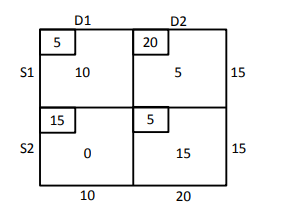
\includegraphics[width=0.75\columnwidth]{chapters/10/7/2/4/figs/fig.png}
 \end{center}
\caption{}
\label{fig:10/7/2/4Fig1}
\end{figure}
\fi

\item Find the position vector of the mid point of the vector joining the points $\vec{P}$(2, 3, 4)
and $\vec{Q}$(4, 1, –2).
\\
\solution
		\begin{enumerate}[label=\thesubsection.\arabic*,ref=\thesubsection.\theenumi]
\item Find the coordinates of the point which divides the join of $(-1,7) $ and $ (4,-3)$ in the ratio 2:3.
	\\
		\solution
	\input{chapters/10/7/2/1/section.tex}
\item Find the coordinates of the point $\vec{R}$ on the line segment joining the points $\vec{P}(-1,3)$ and $\vec{Q}(2,5)$ such that $PR=\frac{3}{5}PQ$.
\item Find the ratio in which the point $\vec{P}\brak{\frac{3}{4},\frac{5}{12}}$ divides the line segment joining the points $\vec{A}\brak{\frac{1}{2},\frac{3}{2}}$ and $ \vec{B}(2,-5)$.
\item Find the coordinates of the point which divides the line segment joining the points $(4,-3)$ and $(8,5)$ in the ratio $3:1$ internally.
\item Find the coordinates of the point $\vec{P}$ on $AD$ such that $AP : PD = 2 : 1$.
\item If the point $\vec{P} (2, 1)$ lies on the line segment joining points $\vec{A} (4, 2)$  and $ \vec{B} (8, 4)$,
then
\begin{enumerate}
	\item $AP =\frac{1}{3}{AB}$ 
\item ${AP}={PE}$
\item ${PB}=\frac{1}{3}{AB}$
\item${AP}=\frac{1}{2}{AB}$
 \end{enumerate}
\item Find the ratio in which the line segment joining the points $(-3,10)$  and  $(6,-8)$  is divided by $ (-1,6)$.
	\\
		\solution
	\input{chapters/10/7/2/4/section.tex}
\item Find the position vector of the mid point of the vector joining the points $\vec{P}$(2, 3, 4)
and $\vec{Q}$(4, 1, –2).
\\
\solution
		\input{chapters/12/10/2/16/section.tex}
\item Let $\vec{A}(4, 2), \vec{B}(6, 5)$  and $ \vec{C}(1, 4)$ be the vertices of $\triangle ABC$.
\begin{enumerate}
\item If $\vec{A}$ and  $\vec{B}$ are $(-2,-2)$ and  $(2,-4)$, respectively, find the coordinates of $\vec{P}$ such that $AP= \frac {3}{7}AB$  and $ \vec{P}$ lies on the line segment $AB$.
	\\
		\solution
	\input{chapters/10/7/2/8/section.tex}
\item Find the coordinates of the points which divide the line segment joining $A(-2,2)$  and  $\vec{B}(2,8)$ into four equal parts.
	\\
		\solution
	\input{chapters/10/7/2/9/section.tex}
\item In what ratio does the point $(-4,6)$ divide the line segment joining the points $\vec{A}(-6,0)$ and $\vec{B}(3,-8)$?
\item Given that $\vec{P}(3,2,-4), \vec{Q}(5,4,-6)$ and $\vec{R}(9,8,-10)$ are collinear. Find the ratio in which $\vec{Q}$ divides $PR$.
\item Points $\vec{A}(-6,10),\vec{B}(-4,6)$  and  $\vec{C}(3,-8)$ are collinear such that $AB=  \frac{2}{9}AC$.
\item The point which divides the line segment joining the points $\vec{P} (7, –6) $  and  $\vec{Q}(3, 4)$ in the 
ratio 1 : 2 internally lies in  which quadrant?
\item Find the coordinates of the points of trisection of the line segment joining $(4,-1)$  and  $(-2,3)$.
	\\
		\solution
	\input{chapters/10/7/2/2/section.tex}
\item Find the coordinates of the points which trisect the line segment joining the points $\vec{P}(4,2,-6)$ and $\vec{Q}(10,-16,6)$.
\item Find the coordinates of the points of trisection (i.e. points dividing to three equal parts) of the line segment joining the points $\vec{A}(2,-2)$ and $\vec{B}(-7,4)$.
\item Point $\vec{P}(5,-3)$ is one of the two points of trisection of line segment joining the points $\vec{A}(7,-2)$ and $\vec{B}(1,-5)$
\item Find the position vector of a point $\vec{R}$ which divides the line joining two points $\vec{P}$
and $\vec{Q}$ whose position vectors are $\hat{i}+2\hat{j}-\hat{k}$ and $-\hat{i}+\hat{j}+\hat{k}$ respectively, in the
ratio 2 : 1
\begin{enumerate}
    \item  internally
    \item  externally
\end{enumerate}
%\solution
%		\input{chapters/12/10/2/15/section.tex}
\item Find the coordinates of the point which divides the line segment joining the points which divides the line segment joining  the points $(-2,3,5)$ and $(1,-4,6)$ in the ratio 
\begin{enumerate}
\item $2:3$ internally,
\item $2:3$ externally
\end{enumerate}
\item Find the coordinates of the point which divides the line segment joining the points $(1,-2,3)$ and $(3,4,-5)$ in the ratio $2:3$
\begin{enumerate}
\item internally, and
\item externally
\end{enumerate}
\item Consider two points $\vec{P}$ and $\vec{Q}$ with position vectors $\overrightarrow{OP} = 3\overrightarrow{a}-2\overrightarrow{b}$ and $\overrightarrow{OQ}=\overrightarrow{a}+\overrightarrow{b}$. Find the position vector of a point $\vec{R}$ which divides the line joining $\vec{P}$ and $\vec{Q}$ in the ratio $2:1$, 
\begin{enumerate}
\item internally, and 
\item externally.
\end{enumerate}
\item The median from $\vec{A}$ meets $BC$ at $\vec{D}$. Find the coordinates of the point $\vec{D}$.
\item Find the coordinates of points $\vec{Q}$ and $\vec{R}$ on medians $BE$ and $CF$ respectively such that $BQ : QE = 2 : 1$  and  $CR : RF = 2 : 1$.
\item What do you observe?
\item If $\vec{A}, \vec{B}$ and $\vec{C}$  are the vertices of $\triangle ABC$, find the coordinates of the centroid of the triangle.
\end{enumerate}
\solution
	\input{chapters/10/7/4/7/section.tex}
\item If $\vec{P}(9a-2,-b)$ divides line segment joining $\vec{A}(3a+1,-3)$ and $\vec{B}(8a,5)$ in the ratio 3:1, find the values of $a$ and $b$.
\item Find the position vector of a point $\vec{R}$ which divides the line joining two points $\vec{P}$ and $\vec{Q}$ whose position vectors are $2\vec{a}+\vec{b}$ and $\vec{a}-3\vec{b}$ externally in the ratio $1:2$.
\item The position vector of the point which divides the join of points 2$\vec{a}$-3$\vec{b}$ $\text{and}$ $\vec{a}+\vec{b}$ in the ratio 3:1 is \rule{1cm}{0.1pt}.
\item If $\vec{a}$ and $\vec{b}$ are the postion vectors of $\vec{A}$ and $\vec{B}$, respectively, find the position vector of a point $\vec{C}$ in $BA$ produced such that $BC=1.5BA$.
\item Find the position vector of a point $\vec{R}$ which divides the line joining two points $\vec{P}$ and $\vec{Q}$ whose position vectors are $(2\vec{a}+\vec{b})$ and $(\vec{a}-3\vec{b})$
externally in the ratio 1 : 2. Also, show that $\vec{P}$ is the mid point of the line segment $RQ$.
\end{enumerate}

\item Let $\vec{A}(4, 2), \vec{B}(6, 5)$  and $ \vec{C}(1, 4)$ be the vertices of $\triangle ABC$.
\begin{enumerate}
\item If $\vec{A}$ and  $\vec{B}$ are $(-2,-2)$ and  $(2,-4)$, respectively, find the coordinates of $\vec{P}$ such that $AP= \frac {3}{7}AB$  and $ \vec{P}$ lies on the line segment $AB$.
	\\
		\solution
	\begin{enumerate}[label=\thesubsection.\arabic*,ref=\thesubsection.\theenumi]
\item Find the coordinates of the point which divides the join of $(-1,7) $ and $ (4,-3)$ in the ratio 2:3.
	\\
		\solution
	\input{chapters/10/7/2/1/section.tex}
\item Find the coordinates of the point $\vec{R}$ on the line segment joining the points $\vec{P}(-1,3)$ and $\vec{Q}(2,5)$ such that $PR=\frac{3}{5}PQ$.
\item Find the ratio in which the point $\vec{P}\brak{\frac{3}{4},\frac{5}{12}}$ divides the line segment joining the points $\vec{A}\brak{\frac{1}{2},\frac{3}{2}}$ and $ \vec{B}(2,-5)$.
\item Find the coordinates of the point which divides the line segment joining the points $(4,-3)$ and $(8,5)$ in the ratio $3:1$ internally.
\item Find the coordinates of the point $\vec{P}$ on $AD$ such that $AP : PD = 2 : 1$.
\item If the point $\vec{P} (2, 1)$ lies on the line segment joining points $\vec{A} (4, 2)$  and $ \vec{B} (8, 4)$,
then
\begin{enumerate}
	\item $AP =\frac{1}{3}{AB}$ 
\item ${AP}={PE}$
\item ${PB}=\frac{1}{3}{AB}$
\item${AP}=\frac{1}{2}{AB}$
 \end{enumerate}
\item Find the ratio in which the line segment joining the points $(-3,10)$  and  $(6,-8)$  is divided by $ (-1,6)$.
	\\
		\solution
	\input{chapters/10/7/2/4/section.tex}
\item Find the position vector of the mid point of the vector joining the points $\vec{P}$(2, 3, 4)
and $\vec{Q}$(4, 1, –2).
\\
\solution
		\input{chapters/12/10/2/16/section.tex}
\item Let $\vec{A}(4, 2), \vec{B}(6, 5)$  and $ \vec{C}(1, 4)$ be the vertices of $\triangle ABC$.
\begin{enumerate}
\item If $\vec{A}$ and  $\vec{B}$ are $(-2,-2)$ and  $(2,-4)$, respectively, find the coordinates of $\vec{P}$ such that $AP= \frac {3}{7}AB$  and $ \vec{P}$ lies on the line segment $AB$.
	\\
		\solution
	\input{chapters/10/7/2/8/section.tex}
\item Find the coordinates of the points which divide the line segment joining $A(-2,2)$  and  $\vec{B}(2,8)$ into four equal parts.
	\\
		\solution
	\input{chapters/10/7/2/9/section.tex}
\item In what ratio does the point $(-4,6)$ divide the line segment joining the points $\vec{A}(-6,0)$ and $\vec{B}(3,-8)$?
\item Given that $\vec{P}(3,2,-4), \vec{Q}(5,4,-6)$ and $\vec{R}(9,8,-10)$ are collinear. Find the ratio in which $\vec{Q}$ divides $PR$.
\item Points $\vec{A}(-6,10),\vec{B}(-4,6)$  and  $\vec{C}(3,-8)$ are collinear such that $AB=  \frac{2}{9}AC$.
\item The point which divides the line segment joining the points $\vec{P} (7, –6) $  and  $\vec{Q}(3, 4)$ in the 
ratio 1 : 2 internally lies in  which quadrant?
\item Find the coordinates of the points of trisection of the line segment joining $(4,-1)$  and  $(-2,3)$.
	\\
		\solution
	\input{chapters/10/7/2/2/section.tex}
\item Find the coordinates of the points which trisect the line segment joining the points $\vec{P}(4,2,-6)$ and $\vec{Q}(10,-16,6)$.
\item Find the coordinates of the points of trisection (i.e. points dividing to three equal parts) of the line segment joining the points $\vec{A}(2,-2)$ and $\vec{B}(-7,4)$.
\item Point $\vec{P}(5,-3)$ is one of the two points of trisection of line segment joining the points $\vec{A}(7,-2)$ and $\vec{B}(1,-5)$
\item Find the position vector of a point $\vec{R}$ which divides the line joining two points $\vec{P}$
and $\vec{Q}$ whose position vectors are $\hat{i}+2\hat{j}-\hat{k}$ and $-\hat{i}+\hat{j}+\hat{k}$ respectively, in the
ratio 2 : 1
\begin{enumerate}
    \item  internally
    \item  externally
\end{enumerate}
%\solution
%		\input{chapters/12/10/2/15/section.tex}
\item Find the coordinates of the point which divides the line segment joining the points which divides the line segment joining  the points $(-2,3,5)$ and $(1,-4,6)$ in the ratio 
\begin{enumerate}
\item $2:3$ internally,
\item $2:3$ externally
\end{enumerate}
\item Find the coordinates of the point which divides the line segment joining the points $(1,-2,3)$ and $(3,4,-5)$ in the ratio $2:3$
\begin{enumerate}
\item internally, and
\item externally
\end{enumerate}
\item Consider two points $\vec{P}$ and $\vec{Q}$ with position vectors $\overrightarrow{OP} = 3\overrightarrow{a}-2\overrightarrow{b}$ and $\overrightarrow{OQ}=\overrightarrow{a}+\overrightarrow{b}$. Find the position vector of a point $\vec{R}$ which divides the line joining $\vec{P}$ and $\vec{Q}$ in the ratio $2:1$, 
\begin{enumerate}
\item internally, and 
\item externally.
\end{enumerate}
\item The median from $\vec{A}$ meets $BC$ at $\vec{D}$. Find the coordinates of the point $\vec{D}$.
\item Find the coordinates of points $\vec{Q}$ and $\vec{R}$ on medians $BE$ and $CF$ respectively such that $BQ : QE = 2 : 1$  and  $CR : RF = 2 : 1$.
\item What do you observe?
\item If $\vec{A}, \vec{B}$ and $\vec{C}$  are the vertices of $\triangle ABC$, find the coordinates of the centroid of the triangle.
\end{enumerate}
\solution
	\input{chapters/10/7/4/7/section.tex}
\item If $\vec{P}(9a-2,-b)$ divides line segment joining $\vec{A}(3a+1,-3)$ and $\vec{B}(8a,5)$ in the ratio 3:1, find the values of $a$ and $b$.
\item Find the position vector of a point $\vec{R}$ which divides the line joining two points $\vec{P}$ and $\vec{Q}$ whose position vectors are $2\vec{a}+\vec{b}$ and $\vec{a}-3\vec{b}$ externally in the ratio $1:2$.
\item The position vector of the point which divides the join of points 2$\vec{a}$-3$\vec{b}$ $\text{and}$ $\vec{a}+\vec{b}$ in the ratio 3:1 is \rule{1cm}{0.1pt}.
\item If $\vec{a}$ and $\vec{b}$ are the postion vectors of $\vec{A}$ and $\vec{B}$, respectively, find the position vector of a point $\vec{C}$ in $BA$ produced such that $BC=1.5BA$.
\item Find the position vector of a point $\vec{R}$ which divides the line joining two points $\vec{P}$ and $\vec{Q}$ whose position vectors are $(2\vec{a}+\vec{b})$ and $(\vec{a}-3\vec{b})$
externally in the ratio 1 : 2. Also, show that $\vec{P}$ is the mid point of the line segment $RQ$.
\end{enumerate}

\item Find the coordinates of the points which divide the line segment joining $A(-2,2)$  and  $\vec{B}(2,8)$ into four equal parts.
	\\
		\solution
	\begin{enumerate}[label=\thesubsection.\arabic*,ref=\thesubsection.\theenumi]
\item Find the coordinates of the point which divides the join of $(-1,7) $ and $ (4,-3)$ in the ratio 2:3.
	\\
		\solution
	\input{chapters/10/7/2/1/section.tex}
\item Find the coordinates of the point $\vec{R}$ on the line segment joining the points $\vec{P}(-1,3)$ and $\vec{Q}(2,5)$ such that $PR=\frac{3}{5}PQ$.
\item Find the ratio in which the point $\vec{P}\brak{\frac{3}{4},\frac{5}{12}}$ divides the line segment joining the points $\vec{A}\brak{\frac{1}{2},\frac{3}{2}}$ and $ \vec{B}(2,-5)$.
\item Find the coordinates of the point which divides the line segment joining the points $(4,-3)$ and $(8,5)$ in the ratio $3:1$ internally.
\item Find the coordinates of the point $\vec{P}$ on $AD$ such that $AP : PD = 2 : 1$.
\item If the point $\vec{P} (2, 1)$ lies on the line segment joining points $\vec{A} (4, 2)$  and $ \vec{B} (8, 4)$,
then
\begin{enumerate}
	\item $AP =\frac{1}{3}{AB}$ 
\item ${AP}={PE}$
\item ${PB}=\frac{1}{3}{AB}$
\item${AP}=\frac{1}{2}{AB}$
 \end{enumerate}
\item Find the ratio in which the line segment joining the points $(-3,10)$  and  $(6,-8)$  is divided by $ (-1,6)$.
	\\
		\solution
	\input{chapters/10/7/2/4/section.tex}
\item Find the position vector of the mid point of the vector joining the points $\vec{P}$(2, 3, 4)
and $\vec{Q}$(4, 1, –2).
\\
\solution
		\input{chapters/12/10/2/16/section.tex}
\item Let $\vec{A}(4, 2), \vec{B}(6, 5)$  and $ \vec{C}(1, 4)$ be the vertices of $\triangle ABC$.
\begin{enumerate}
\item If $\vec{A}$ and  $\vec{B}$ are $(-2,-2)$ and  $(2,-4)$, respectively, find the coordinates of $\vec{P}$ such that $AP= \frac {3}{7}AB$  and $ \vec{P}$ lies on the line segment $AB$.
	\\
		\solution
	\input{chapters/10/7/2/8/section.tex}
\item Find the coordinates of the points which divide the line segment joining $A(-2,2)$  and  $\vec{B}(2,8)$ into four equal parts.
	\\
		\solution
	\input{chapters/10/7/2/9/section.tex}
\item In what ratio does the point $(-4,6)$ divide the line segment joining the points $\vec{A}(-6,0)$ and $\vec{B}(3,-8)$?
\item Given that $\vec{P}(3,2,-4), \vec{Q}(5,4,-6)$ and $\vec{R}(9,8,-10)$ are collinear. Find the ratio in which $\vec{Q}$ divides $PR$.
\item Points $\vec{A}(-6,10),\vec{B}(-4,6)$  and  $\vec{C}(3,-8)$ are collinear such that $AB=  \frac{2}{9}AC$.
\item The point which divides the line segment joining the points $\vec{P} (7, –6) $  and  $\vec{Q}(3, 4)$ in the 
ratio 1 : 2 internally lies in  which quadrant?
\item Find the coordinates of the points of trisection of the line segment joining $(4,-1)$  and  $(-2,3)$.
	\\
		\solution
	\input{chapters/10/7/2/2/section.tex}
\item Find the coordinates of the points which trisect the line segment joining the points $\vec{P}(4,2,-6)$ and $\vec{Q}(10,-16,6)$.
\item Find the coordinates of the points of trisection (i.e. points dividing to three equal parts) of the line segment joining the points $\vec{A}(2,-2)$ and $\vec{B}(-7,4)$.
\item Point $\vec{P}(5,-3)$ is one of the two points of trisection of line segment joining the points $\vec{A}(7,-2)$ and $\vec{B}(1,-5)$
\item Find the position vector of a point $\vec{R}$ which divides the line joining two points $\vec{P}$
and $\vec{Q}$ whose position vectors are $\hat{i}+2\hat{j}-\hat{k}$ and $-\hat{i}+\hat{j}+\hat{k}$ respectively, in the
ratio 2 : 1
\begin{enumerate}
    \item  internally
    \item  externally
\end{enumerate}
%\solution
%		\input{chapters/12/10/2/15/section.tex}
\item Find the coordinates of the point which divides the line segment joining the points which divides the line segment joining  the points $(-2,3,5)$ and $(1,-4,6)$ in the ratio 
\begin{enumerate}
\item $2:3$ internally,
\item $2:3$ externally
\end{enumerate}
\item Find the coordinates of the point which divides the line segment joining the points $(1,-2,3)$ and $(3,4,-5)$ in the ratio $2:3$
\begin{enumerate}
\item internally, and
\item externally
\end{enumerate}
\item Consider two points $\vec{P}$ and $\vec{Q}$ with position vectors $\overrightarrow{OP} = 3\overrightarrow{a}-2\overrightarrow{b}$ and $\overrightarrow{OQ}=\overrightarrow{a}+\overrightarrow{b}$. Find the position vector of a point $\vec{R}$ which divides the line joining $\vec{P}$ and $\vec{Q}$ in the ratio $2:1$, 
\begin{enumerate}
\item internally, and 
\item externally.
\end{enumerate}
\item The median from $\vec{A}$ meets $BC$ at $\vec{D}$. Find the coordinates of the point $\vec{D}$.
\item Find the coordinates of points $\vec{Q}$ and $\vec{R}$ on medians $BE$ and $CF$ respectively such that $BQ : QE = 2 : 1$  and  $CR : RF = 2 : 1$.
\item What do you observe?
\item If $\vec{A}, \vec{B}$ and $\vec{C}$  are the vertices of $\triangle ABC$, find the coordinates of the centroid of the triangle.
\end{enumerate}
\solution
	\input{chapters/10/7/4/7/section.tex}
\item If $\vec{P}(9a-2,-b)$ divides line segment joining $\vec{A}(3a+1,-3)$ and $\vec{B}(8a,5)$ in the ratio 3:1, find the values of $a$ and $b$.
\item Find the position vector of a point $\vec{R}$ which divides the line joining two points $\vec{P}$ and $\vec{Q}$ whose position vectors are $2\vec{a}+\vec{b}$ and $\vec{a}-3\vec{b}$ externally in the ratio $1:2$.
\item The position vector of the point which divides the join of points 2$\vec{a}$-3$\vec{b}$ $\text{and}$ $\vec{a}+\vec{b}$ in the ratio 3:1 is \rule{1cm}{0.1pt}.
\item If $\vec{a}$ and $\vec{b}$ are the postion vectors of $\vec{A}$ and $\vec{B}$, respectively, find the position vector of a point $\vec{C}$ in $BA$ produced such that $BC=1.5BA$.
\item Find the position vector of a point $\vec{R}$ which divides the line joining two points $\vec{P}$ and $\vec{Q}$ whose position vectors are $(2\vec{a}+\vec{b})$ and $(\vec{a}-3\vec{b})$
externally in the ratio 1 : 2. Also, show that $\vec{P}$ is the mid point of the line segment $RQ$.
\end{enumerate}

\item In what ratio does the point $(-4,6)$ divide the line segment joining the points $\vec{A}(-6,0)$ and $\vec{B}(3,-8)$?
\item Given that $\vec{P}(3,2,-4), \vec{Q}(5,4,-6)$ and $\vec{R}(9,8,-10)$ are collinear. Find the ratio in which $\vec{Q}$ divides $PR$.
\item Points $\vec{A}(-6,10),\vec{B}(-4,6)$  and  $\vec{C}(3,-8)$ are collinear such that $AB=  \frac{2}{9}AC$.
\item The point which divides the line segment joining the points $\vec{P} (7, –6) $  and  $\vec{Q}(3, 4)$ in the 
ratio 1 : 2 internally lies in  which quadrant?
\item Find the coordinates of the points of trisection of the line segment joining $(4,-1)$  and  $(-2,3)$.
	\\
		\solution
	Using section formula,
\begin{align}
\vec{R}=\frac{1}{1+\frac{1}{2}}\brak{\myvec{4\\-1}+\frac{1}{2}\myvec{-2\\3}}
=\myvec{2\\ \frac{1}{3}}\\
\vec{S}=\frac{1}{1+\frac{2}{1}}\brak{\myvec{4\\-1}+\frac{2}{1}\myvec{-2\\3}}
=\myvec{0\\ \frac{5}{3}}
\end{align}
which are the desired points of trisection.
\iffalse
See
		\figref{fig:chapters/10/7/2/2/Figure}
\begin{figure}[H]
\centering
\includegraphics[width=0.75\columnwidth]{chapters/10/7/2/2/figs/dj.pdf}
\caption{}
		\label{fig:chapters/10/7/2/2/Figure}
\end{figure}
\fi

\item Find the coordinates of the points which trisect the line segment joining the points $\vec{P}(4,2,-6)$ and $\vec{Q}(10,-16,6)$.
\item Find the coordinates of the points of trisection (i.e. points dividing to three equal parts) of the line segment joining the points $\vec{A}(2,-2)$ and $\vec{B}(-7,4)$.
\item Point $\vec{P}(5,-3)$ is one of the two points of trisection of line segment joining the points $\vec{A}(7,-2)$ and $\vec{B}(1,-5)$
\item Find the position vector of a point $\vec{R}$ which divides the line joining two points $\vec{P}$
and $\vec{Q}$ whose position vectors are $\hat{i}+2\hat{j}-\hat{k}$ and $-\hat{i}+\hat{j}+\hat{k}$ respectively, in the
ratio 2 : 1
\begin{enumerate}
    \item  internally
    \item  externally
\end{enumerate}
%\solution
%		\begin{enumerate}[label=\thesubsection.\arabic*,ref=\thesubsection.\theenumi]
\item Find the coordinates of the point which divides the join of $(-1,7) $ and $ (4,-3)$ in the ratio 2:3.
	\\
		\solution
	\input{chapters/10/7/2/1/section.tex}
\item Find the coordinates of the point $\vec{R}$ on the line segment joining the points $\vec{P}(-1,3)$ and $\vec{Q}(2,5)$ such that $PR=\frac{3}{5}PQ$.
\item Find the ratio in which the point $\vec{P}\brak{\frac{3}{4},\frac{5}{12}}$ divides the line segment joining the points $\vec{A}\brak{\frac{1}{2},\frac{3}{2}}$ and $ \vec{B}(2,-5)$.
\item Find the coordinates of the point which divides the line segment joining the points $(4,-3)$ and $(8,5)$ in the ratio $3:1$ internally.
\item Find the coordinates of the point $\vec{P}$ on $AD$ such that $AP : PD = 2 : 1$.
\item If the point $\vec{P} (2, 1)$ lies on the line segment joining points $\vec{A} (4, 2)$  and $ \vec{B} (8, 4)$,
then
\begin{enumerate}
	\item $AP =\frac{1}{3}{AB}$ 
\item ${AP}={PE}$
\item ${PB}=\frac{1}{3}{AB}$
\item${AP}=\frac{1}{2}{AB}$
 \end{enumerate}
\item Find the ratio in which the line segment joining the points $(-3,10)$  and  $(6,-8)$  is divided by $ (-1,6)$.
	\\
		\solution
	\input{chapters/10/7/2/4/section.tex}
\item Find the position vector of the mid point of the vector joining the points $\vec{P}$(2, 3, 4)
and $\vec{Q}$(4, 1, –2).
\\
\solution
		\input{chapters/12/10/2/16/section.tex}
\item Let $\vec{A}(4, 2), \vec{B}(6, 5)$  and $ \vec{C}(1, 4)$ be the vertices of $\triangle ABC$.
\begin{enumerate}
\item If $\vec{A}$ and  $\vec{B}$ are $(-2,-2)$ and  $(2,-4)$, respectively, find the coordinates of $\vec{P}$ such that $AP= \frac {3}{7}AB$  and $ \vec{P}$ lies on the line segment $AB$.
	\\
		\solution
	\input{chapters/10/7/2/8/section.tex}
\item Find the coordinates of the points which divide the line segment joining $A(-2,2)$  and  $\vec{B}(2,8)$ into four equal parts.
	\\
		\solution
	\input{chapters/10/7/2/9/section.tex}
\item In what ratio does the point $(-4,6)$ divide the line segment joining the points $\vec{A}(-6,0)$ and $\vec{B}(3,-8)$?
\item Given that $\vec{P}(3,2,-4), \vec{Q}(5,4,-6)$ and $\vec{R}(9,8,-10)$ are collinear. Find the ratio in which $\vec{Q}$ divides $PR$.
\item Points $\vec{A}(-6,10),\vec{B}(-4,6)$  and  $\vec{C}(3,-8)$ are collinear such that $AB=  \frac{2}{9}AC$.
\item The point which divides the line segment joining the points $\vec{P} (7, –6) $  and  $\vec{Q}(3, 4)$ in the 
ratio 1 : 2 internally lies in  which quadrant?
\item Find the coordinates of the points of trisection of the line segment joining $(4,-1)$  and  $(-2,3)$.
	\\
		\solution
	\input{chapters/10/7/2/2/section.tex}
\item Find the coordinates of the points which trisect the line segment joining the points $\vec{P}(4,2,-6)$ and $\vec{Q}(10,-16,6)$.
\item Find the coordinates of the points of trisection (i.e. points dividing to three equal parts) of the line segment joining the points $\vec{A}(2,-2)$ and $\vec{B}(-7,4)$.
\item Point $\vec{P}(5,-3)$ is one of the two points of trisection of line segment joining the points $\vec{A}(7,-2)$ and $\vec{B}(1,-5)$
\item Find the position vector of a point $\vec{R}$ which divides the line joining two points $\vec{P}$
and $\vec{Q}$ whose position vectors are $\hat{i}+2\hat{j}-\hat{k}$ and $-\hat{i}+\hat{j}+\hat{k}$ respectively, in the
ratio 2 : 1
\begin{enumerate}
    \item  internally
    \item  externally
\end{enumerate}
%\solution
%		\input{chapters/12/10/2/15/section.tex}
\item Find the coordinates of the point which divides the line segment joining the points which divides the line segment joining  the points $(-2,3,5)$ and $(1,-4,6)$ in the ratio 
\begin{enumerate}
\item $2:3$ internally,
\item $2:3$ externally
\end{enumerate}
\item Find the coordinates of the point which divides the line segment joining the points $(1,-2,3)$ and $(3,4,-5)$ in the ratio $2:3$
\begin{enumerate}
\item internally, and
\item externally
\end{enumerate}
\item Consider two points $\vec{P}$ and $\vec{Q}$ with position vectors $\overrightarrow{OP} = 3\overrightarrow{a}-2\overrightarrow{b}$ and $\overrightarrow{OQ}=\overrightarrow{a}+\overrightarrow{b}$. Find the position vector of a point $\vec{R}$ which divides the line joining $\vec{P}$ and $\vec{Q}$ in the ratio $2:1$, 
\begin{enumerate}
\item internally, and 
\item externally.
\end{enumerate}
\item The median from $\vec{A}$ meets $BC$ at $\vec{D}$. Find the coordinates of the point $\vec{D}$.
\item Find the coordinates of points $\vec{Q}$ and $\vec{R}$ on medians $BE$ and $CF$ respectively such that $BQ : QE = 2 : 1$  and  $CR : RF = 2 : 1$.
\item What do you observe?
\item If $\vec{A}, \vec{B}$ and $\vec{C}$  are the vertices of $\triangle ABC$, find the coordinates of the centroid of the triangle.
\end{enumerate}
\solution
	\input{chapters/10/7/4/7/section.tex}
\item If $\vec{P}(9a-2,-b)$ divides line segment joining $\vec{A}(3a+1,-3)$ and $\vec{B}(8a,5)$ in the ratio 3:1, find the values of $a$ and $b$.
\item Find the position vector of a point $\vec{R}$ which divides the line joining two points $\vec{P}$ and $\vec{Q}$ whose position vectors are $2\vec{a}+\vec{b}$ and $\vec{a}-3\vec{b}$ externally in the ratio $1:2$.
\item The position vector of the point which divides the join of points 2$\vec{a}$-3$\vec{b}$ $\text{and}$ $\vec{a}+\vec{b}$ in the ratio 3:1 is \rule{1cm}{0.1pt}.
\item If $\vec{a}$ and $\vec{b}$ are the postion vectors of $\vec{A}$ and $\vec{B}$, respectively, find the position vector of a point $\vec{C}$ in $BA$ produced such that $BC=1.5BA$.
\item Find the position vector of a point $\vec{R}$ which divides the line joining two points $\vec{P}$ and $\vec{Q}$ whose position vectors are $(2\vec{a}+\vec{b})$ and $(\vec{a}-3\vec{b})$
externally in the ratio 1 : 2. Also, show that $\vec{P}$ is the mid point of the line segment $RQ$.
\end{enumerate}

\item Find the coordinates of the point which divides the line segment joining the points which divides the line segment joining  the points $(-2,3,5)$ and $(1,-4,6)$ in the ratio 
\begin{enumerate}
\item $2:3$ internally,
\item $2:3$ externally
\end{enumerate}
\item Find the coordinates of the point which divides the line segment joining the points $(1,-2,3)$ and $(3,4,-5)$ in the ratio $2:3$
\begin{enumerate}
\item internally, and
\item externally
\end{enumerate}
\item Consider two points $\vec{P}$ and $\vec{Q}$ with position vectors $\overrightarrow{OP} = 3\overrightarrow{a}-2\overrightarrow{b}$ and $\overrightarrow{OQ}=\overrightarrow{a}+\overrightarrow{b}$. Find the position vector of a point $\vec{R}$ which divides the line joining $\vec{P}$ and $\vec{Q}$ in the ratio $2:1$, 
\begin{enumerate}
\item internally, and 
\item externally.
\end{enumerate}
\item The median from $\vec{A}$ meets $BC$ at $\vec{D}$. Find the coordinates of the point $\vec{D}$.
\item Find the coordinates of points $\vec{Q}$ and $\vec{R}$ on medians $BE$ and $CF$ respectively such that $BQ : QE = 2 : 1$  and  $CR : RF = 2 : 1$.
\item What do you observe?
\item If $\vec{A}, \vec{B}$ and $\vec{C}$  are the vertices of $\triangle ABC$, find the coordinates of the centroid of the triangle.
\end{enumerate}
\solution
	\begin{enumerate}[label=\thesubsection.\arabic*,ref=\thesubsection.\theenumi]
\item Find the coordinates of the point which divides the join of $(-1,7) $ and $ (4,-3)$ in the ratio 2:3.
	\\
		\solution
	\input{chapters/10/7/2/1/section.tex}
\item Find the coordinates of the point $\vec{R}$ on the line segment joining the points $\vec{P}(-1,3)$ and $\vec{Q}(2,5)$ such that $PR=\frac{3}{5}PQ$.
\item Find the ratio in which the point $\vec{P}\brak{\frac{3}{4},\frac{5}{12}}$ divides the line segment joining the points $\vec{A}\brak{\frac{1}{2},\frac{3}{2}}$ and $ \vec{B}(2,-5)$.
\item Find the coordinates of the point which divides the line segment joining the points $(4,-3)$ and $(8,5)$ in the ratio $3:1$ internally.
\item Find the coordinates of the point $\vec{P}$ on $AD$ such that $AP : PD = 2 : 1$.
\item If the point $\vec{P} (2, 1)$ lies on the line segment joining points $\vec{A} (4, 2)$  and $ \vec{B} (8, 4)$,
then
\begin{enumerate}
	\item $AP =\frac{1}{3}{AB}$ 
\item ${AP}={PE}$
\item ${PB}=\frac{1}{3}{AB}$
\item${AP}=\frac{1}{2}{AB}$
 \end{enumerate}
\item Find the ratio in which the line segment joining the points $(-3,10)$  and  $(6,-8)$  is divided by $ (-1,6)$.
	\\
		\solution
	\input{chapters/10/7/2/4/section.tex}
\item Find the position vector of the mid point of the vector joining the points $\vec{P}$(2, 3, 4)
and $\vec{Q}$(4, 1, –2).
\\
\solution
		\input{chapters/12/10/2/16/section.tex}
\item Let $\vec{A}(4, 2), \vec{B}(6, 5)$  and $ \vec{C}(1, 4)$ be the vertices of $\triangle ABC$.
\begin{enumerate}
\item If $\vec{A}$ and  $\vec{B}$ are $(-2,-2)$ and  $(2,-4)$, respectively, find the coordinates of $\vec{P}$ such that $AP= \frac {3}{7}AB$  and $ \vec{P}$ lies on the line segment $AB$.
	\\
		\solution
	\input{chapters/10/7/2/8/section.tex}
\item Find the coordinates of the points which divide the line segment joining $A(-2,2)$  and  $\vec{B}(2,8)$ into four equal parts.
	\\
		\solution
	\input{chapters/10/7/2/9/section.tex}
\item In what ratio does the point $(-4,6)$ divide the line segment joining the points $\vec{A}(-6,0)$ and $\vec{B}(3,-8)$?
\item Given that $\vec{P}(3,2,-4), \vec{Q}(5,4,-6)$ and $\vec{R}(9,8,-10)$ are collinear. Find the ratio in which $\vec{Q}$ divides $PR$.
\item Points $\vec{A}(-6,10),\vec{B}(-4,6)$  and  $\vec{C}(3,-8)$ are collinear such that $AB=  \frac{2}{9}AC$.
\item The point which divides the line segment joining the points $\vec{P} (7, –6) $  and  $\vec{Q}(3, 4)$ in the 
ratio 1 : 2 internally lies in  which quadrant?
\item Find the coordinates of the points of trisection of the line segment joining $(4,-1)$  and  $(-2,3)$.
	\\
		\solution
	\input{chapters/10/7/2/2/section.tex}
\item Find the coordinates of the points which trisect the line segment joining the points $\vec{P}(4,2,-6)$ and $\vec{Q}(10,-16,6)$.
\item Find the coordinates of the points of trisection (i.e. points dividing to three equal parts) of the line segment joining the points $\vec{A}(2,-2)$ and $\vec{B}(-7,4)$.
\item Point $\vec{P}(5,-3)$ is one of the two points of trisection of line segment joining the points $\vec{A}(7,-2)$ and $\vec{B}(1,-5)$
\item Find the position vector of a point $\vec{R}$ which divides the line joining two points $\vec{P}$
and $\vec{Q}$ whose position vectors are $\hat{i}+2\hat{j}-\hat{k}$ and $-\hat{i}+\hat{j}+\hat{k}$ respectively, in the
ratio 2 : 1
\begin{enumerate}
    \item  internally
    \item  externally
\end{enumerate}
%\solution
%		\input{chapters/12/10/2/15/section.tex}
\item Find the coordinates of the point which divides the line segment joining the points which divides the line segment joining  the points $(-2,3,5)$ and $(1,-4,6)$ in the ratio 
\begin{enumerate}
\item $2:3$ internally,
\item $2:3$ externally
\end{enumerate}
\item Find the coordinates of the point which divides the line segment joining the points $(1,-2,3)$ and $(3,4,-5)$ in the ratio $2:3$
\begin{enumerate}
\item internally, and
\item externally
\end{enumerate}
\item Consider two points $\vec{P}$ and $\vec{Q}$ with position vectors $\overrightarrow{OP} = 3\overrightarrow{a}-2\overrightarrow{b}$ and $\overrightarrow{OQ}=\overrightarrow{a}+\overrightarrow{b}$. Find the position vector of a point $\vec{R}$ which divides the line joining $\vec{P}$ and $\vec{Q}$ in the ratio $2:1$, 
\begin{enumerate}
\item internally, and 
\item externally.
\end{enumerate}
\item The median from $\vec{A}$ meets $BC$ at $\vec{D}$. Find the coordinates of the point $\vec{D}$.
\item Find the coordinates of points $\vec{Q}$ and $\vec{R}$ on medians $BE$ and $CF$ respectively such that $BQ : QE = 2 : 1$  and  $CR : RF = 2 : 1$.
\item What do you observe?
\item If $\vec{A}, \vec{B}$ and $\vec{C}$  are the vertices of $\triangle ABC$, find the coordinates of the centroid of the triangle.
\end{enumerate}
\solution
	\input{chapters/10/7/4/7/section.tex}
\item If $\vec{P}(9a-2,-b)$ divides line segment joining $\vec{A}(3a+1,-3)$ and $\vec{B}(8a,5)$ in the ratio 3:1, find the values of $a$ and $b$.
\item Find the position vector of a point $\vec{R}$ which divides the line joining two points $\vec{P}$ and $\vec{Q}$ whose position vectors are $2\vec{a}+\vec{b}$ and $\vec{a}-3\vec{b}$ externally in the ratio $1:2$.
\item The position vector of the point which divides the join of points 2$\vec{a}$-3$\vec{b}$ $\text{and}$ $\vec{a}+\vec{b}$ in the ratio 3:1 is \rule{1cm}{0.1pt}.
\item If $\vec{a}$ and $\vec{b}$ are the postion vectors of $\vec{A}$ and $\vec{B}$, respectively, find the position vector of a point $\vec{C}$ in $BA$ produced such that $BC=1.5BA$.
\item Find the position vector of a point $\vec{R}$ which divides the line joining two points $\vec{P}$ and $\vec{Q}$ whose position vectors are $(2\vec{a}+\vec{b})$ and $(\vec{a}-3\vec{b})$
externally in the ratio 1 : 2. Also, show that $\vec{P}$ is the mid point of the line segment $RQ$.
\end{enumerate}

\item If $\vec{P}(9a-2,-b)$ divides line segment joining $\vec{A}(3a+1,-3)$ and $\vec{B}(8a,5)$ in the ratio 3:1, find the values of $a$ and $b$.
\item Find the position vector of a point $\vec{R}$ which divides the line joining two points $\vec{P}$ and $\vec{Q}$ whose position vectors are $2\vec{a}+\vec{b}$ and $\vec{a}-3\vec{b}$ externally in the ratio $1:2$.
\item The position vector of the point which divides the join of points 2$\vec{a}$-3$\vec{b}$ $\text{and}$ $\vec{a}+\vec{b}$ in the ratio 3:1 is \rule{1cm}{0.1pt}.
\item If $\vec{a}$ and $\vec{b}$ are the postion vectors of $\vec{A}$ and $\vec{B}$, respectively, find the position vector of a point $\vec{C}$ in $BA$ produced such that $BC=1.5BA$.
\item Find the position vector of a point $\vec{R}$ which divides the line joining two points $\vec{P}$ and $\vec{Q}$ whose position vectors are $(2\vec{a}+\vec{b})$ and $(\vec{a}-3\vec{b})$
externally in the ratio 1 : 2. Also, show that $\vec{P}$ is the mid point of the line segment $RQ$.
\end{enumerate}

\item Find the coordinates of the point $\vec{R}$ on the line segment joining the points $\vec{P}(-1,3)$ and $\vec{Q}(2,5)$ such that $PR=\frac{3}{5}PQ$.
\item Find the ratio in which the point $\vec{P}\brak{\frac{3}{4},\frac{5}{12}}$ divides the line segment joining the points $\vec{A}\brak{\frac{1}{2},\frac{3}{2}}$ and $ \vec{B}(2,-5)$.
\item Find the coordinates of the point which divides the line segment joining the points $(4,-3)$ and $(8,5)$ in the ratio $3:1$ internally.
\item Find the coordinates of the point $\vec{P}$ on $AD$ such that $AP : PD = 2 : 1$.
\item If the point $\vec{P} (2, 1)$ lies on the line segment joining points $\vec{A} (4, 2)$  and $ \vec{B} (8, 4)$,
then
\begin{enumerate}
	\item $AP =\frac{1}{3}{AB}$ 
\item ${AP}={PE}$
\item ${PB}=\frac{1}{3}{AB}$
\item${AP}=\frac{1}{2}{AB}$
 \end{enumerate}
\item Find the ratio in which the line segment joining the points $(-3,10)$  and  $(6,-8)$  is divided by $ (-1,6)$.
	\\
		\solution
	\iffalse
Using section formula,
\begin{align}
         \myvec{-1\\6} &=\frac{{\myvec{-3\\10}+k\myvec{6\\-8}}}{1+k}\\
	 \implies 7k\myvec{1 \\ -2} &= 2\myvec{1 \\ -2}
	 \\
	 \text{or, } k &= \frac{2}{7}.
\end{align}
\fi
In 
			\eqref{eq:section_formula-k}, substituting
			\begin{align}
				\vec{B} &= \myvec{-3\\10}, \vec{C} = \myvec{6\\-8}, \vec{D} = \myvec{-1\\6},
				\\
				k &= \frac{\myvec{-2 & 4}\myvec{-7 \\ 14}}{\norm{\myvec{-7 \\ 14}}^2} = \frac{2}{7}
			\end{align}
\iffalse
See \figref{fig:10/7/2/4Fig1}.
\begin{figure}[H]
 \begin{center}
  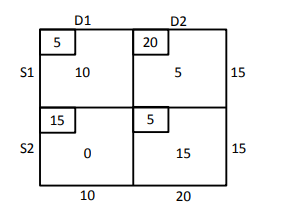
\includegraphics[width=0.75\columnwidth]{chapters/10/7/2/4/figs/fig.png}
 \end{center}
\caption{}
\label{fig:10/7/2/4Fig1}
\end{figure}
\fi

\item Find the position vector of the mid point of the vector joining the points $\vec{P}$(2, 3, 4)
and $\vec{Q}$(4, 1, –2).
\\
\solution
		\begin{enumerate}[label=\thesubsection.\arabic*,ref=\thesubsection.\theenumi]
\item Find the coordinates of the point which divides the join of $(-1,7) $ and $ (4,-3)$ in the ratio 2:3.
	\\
		\solution
	\begin{enumerate}[label=\thesubsection.\arabic*,ref=\thesubsection.\theenumi]
\item Find the coordinates of the point which divides the join of $(-1,7) $ and $ (4,-3)$ in the ratio 2:3.
	\\
		\solution
	\input{chapters/10/7/2/1/section.tex}
\item Find the coordinates of the point $\vec{R}$ on the line segment joining the points $\vec{P}(-1,3)$ and $\vec{Q}(2,5)$ such that $PR=\frac{3}{5}PQ$.
\item Find the ratio in which the point $\vec{P}\brak{\frac{3}{4},\frac{5}{12}}$ divides the line segment joining the points $\vec{A}\brak{\frac{1}{2},\frac{3}{2}}$ and $ \vec{B}(2,-5)$.
\item Find the coordinates of the point which divides the line segment joining the points $(4,-3)$ and $(8,5)$ in the ratio $3:1$ internally.
\item Find the coordinates of the point $\vec{P}$ on $AD$ such that $AP : PD = 2 : 1$.
\item If the point $\vec{P} (2, 1)$ lies on the line segment joining points $\vec{A} (4, 2)$  and $ \vec{B} (8, 4)$,
then
\begin{enumerate}
	\item $AP =\frac{1}{3}{AB}$ 
\item ${AP}={PE}$
\item ${PB}=\frac{1}{3}{AB}$
\item${AP}=\frac{1}{2}{AB}$
 \end{enumerate}
\item Find the ratio in which the line segment joining the points $(-3,10)$  and  $(6,-8)$  is divided by $ (-1,6)$.
	\\
		\solution
	\input{chapters/10/7/2/4/section.tex}
\item Find the position vector of the mid point of the vector joining the points $\vec{P}$(2, 3, 4)
and $\vec{Q}$(4, 1, –2).
\\
\solution
		\input{chapters/12/10/2/16/section.tex}
\item Let $\vec{A}(4, 2), \vec{B}(6, 5)$  and $ \vec{C}(1, 4)$ be the vertices of $\triangle ABC$.
\begin{enumerate}
\item If $\vec{A}$ and  $\vec{B}$ are $(-2,-2)$ and  $(2,-4)$, respectively, find the coordinates of $\vec{P}$ such that $AP= \frac {3}{7}AB$  and $ \vec{P}$ lies on the line segment $AB$.
	\\
		\solution
	\input{chapters/10/7/2/8/section.tex}
\item Find the coordinates of the points which divide the line segment joining $A(-2,2)$  and  $\vec{B}(2,8)$ into four equal parts.
	\\
		\solution
	\input{chapters/10/7/2/9/section.tex}
\item In what ratio does the point $(-4,6)$ divide the line segment joining the points $\vec{A}(-6,0)$ and $\vec{B}(3,-8)$?
\item Given that $\vec{P}(3,2,-4), \vec{Q}(5,4,-6)$ and $\vec{R}(9,8,-10)$ are collinear. Find the ratio in which $\vec{Q}$ divides $PR$.
\item Points $\vec{A}(-6,10),\vec{B}(-4,6)$  and  $\vec{C}(3,-8)$ are collinear such that $AB=  \frac{2}{9}AC$.
\item The point which divides the line segment joining the points $\vec{P} (7, –6) $  and  $\vec{Q}(3, 4)$ in the 
ratio 1 : 2 internally lies in  which quadrant?
\item Find the coordinates of the points of trisection of the line segment joining $(4,-1)$  and  $(-2,3)$.
	\\
		\solution
	\input{chapters/10/7/2/2/section.tex}
\item Find the coordinates of the points which trisect the line segment joining the points $\vec{P}(4,2,-6)$ and $\vec{Q}(10,-16,6)$.
\item Find the coordinates of the points of trisection (i.e. points dividing to three equal parts) of the line segment joining the points $\vec{A}(2,-2)$ and $\vec{B}(-7,4)$.
\item Point $\vec{P}(5,-3)$ is one of the two points of trisection of line segment joining the points $\vec{A}(7,-2)$ and $\vec{B}(1,-5)$
\item Find the position vector of a point $\vec{R}$ which divides the line joining two points $\vec{P}$
and $\vec{Q}$ whose position vectors are $\hat{i}+2\hat{j}-\hat{k}$ and $-\hat{i}+\hat{j}+\hat{k}$ respectively, in the
ratio 2 : 1
\begin{enumerate}
    \item  internally
    \item  externally
\end{enumerate}
%\solution
%		\input{chapters/12/10/2/15/section.tex}
\item Find the coordinates of the point which divides the line segment joining the points which divides the line segment joining  the points $(-2,3,5)$ and $(1,-4,6)$ in the ratio 
\begin{enumerate}
\item $2:3$ internally,
\item $2:3$ externally
\end{enumerate}
\item Find the coordinates of the point which divides the line segment joining the points $(1,-2,3)$ and $(3,4,-5)$ in the ratio $2:3$
\begin{enumerate}
\item internally, and
\item externally
\end{enumerate}
\item Consider two points $\vec{P}$ and $\vec{Q}$ with position vectors $\overrightarrow{OP} = 3\overrightarrow{a}-2\overrightarrow{b}$ and $\overrightarrow{OQ}=\overrightarrow{a}+\overrightarrow{b}$. Find the position vector of a point $\vec{R}$ which divides the line joining $\vec{P}$ and $\vec{Q}$ in the ratio $2:1$, 
\begin{enumerate}
\item internally, and 
\item externally.
\end{enumerate}
\item The median from $\vec{A}$ meets $BC$ at $\vec{D}$. Find the coordinates of the point $\vec{D}$.
\item Find the coordinates of points $\vec{Q}$ and $\vec{R}$ on medians $BE$ and $CF$ respectively such that $BQ : QE = 2 : 1$  and  $CR : RF = 2 : 1$.
\item What do you observe?
\item If $\vec{A}, \vec{B}$ and $\vec{C}$  are the vertices of $\triangle ABC$, find the coordinates of the centroid of the triangle.
\end{enumerate}
\solution
	\input{chapters/10/7/4/7/section.tex}
\item If $\vec{P}(9a-2,-b)$ divides line segment joining $\vec{A}(3a+1,-3)$ and $\vec{B}(8a,5)$ in the ratio 3:1, find the values of $a$ and $b$.
\item Find the position vector of a point $\vec{R}$ which divides the line joining two points $\vec{P}$ and $\vec{Q}$ whose position vectors are $2\vec{a}+\vec{b}$ and $\vec{a}-3\vec{b}$ externally in the ratio $1:2$.
\item The position vector of the point which divides the join of points 2$\vec{a}$-3$\vec{b}$ $\text{and}$ $\vec{a}+\vec{b}$ in the ratio 3:1 is \rule{1cm}{0.1pt}.
\item If $\vec{a}$ and $\vec{b}$ are the postion vectors of $\vec{A}$ and $\vec{B}$, respectively, find the position vector of a point $\vec{C}$ in $BA$ produced such that $BC=1.5BA$.
\item Find the position vector of a point $\vec{R}$ which divides the line joining two points $\vec{P}$ and $\vec{Q}$ whose position vectors are $(2\vec{a}+\vec{b})$ and $(\vec{a}-3\vec{b})$
externally in the ratio 1 : 2. Also, show that $\vec{P}$ is the mid point of the line segment $RQ$.
\end{enumerate}

\item Find the coordinates of the point $\vec{R}$ on the line segment joining the points $\vec{P}(-1,3)$ and $\vec{Q}(2,5)$ such that $PR=\frac{3}{5}PQ$.
\item Find the ratio in which the point $\vec{P}\brak{\frac{3}{4},\frac{5}{12}}$ divides the line segment joining the points $\vec{A}\brak{\frac{1}{2},\frac{3}{2}}$ and $ \vec{B}(2,-5)$.
\item Find the coordinates of the point which divides the line segment joining the points $(4,-3)$ and $(8,5)$ in the ratio $3:1$ internally.
\item Find the coordinates of the point $\vec{P}$ on $AD$ such that $AP : PD = 2 : 1$.
\item If the point $\vec{P} (2, 1)$ lies on the line segment joining points $\vec{A} (4, 2)$  and $ \vec{B} (8, 4)$,
then
\begin{enumerate}
	\item $AP =\frac{1}{3}{AB}$ 
\item ${AP}={PE}$
\item ${PB}=\frac{1}{3}{AB}$
\item${AP}=\frac{1}{2}{AB}$
 \end{enumerate}
\item Find the ratio in which the line segment joining the points $(-3,10)$  and  $(6,-8)$  is divided by $ (-1,6)$.
	\\
		\solution
	\iffalse
Using section formula,
\begin{align}
         \myvec{-1\\6} &=\frac{{\myvec{-3\\10}+k\myvec{6\\-8}}}{1+k}\\
	 \implies 7k\myvec{1 \\ -2} &= 2\myvec{1 \\ -2}
	 \\
	 \text{or, } k &= \frac{2}{7}.
\end{align}
\fi
In 
			\eqref{eq:section_formula-k}, substituting
			\begin{align}
				\vec{B} &= \myvec{-3\\10}, \vec{C} = \myvec{6\\-8}, \vec{D} = \myvec{-1\\6},
				\\
				k &= \frac{\myvec{-2 & 4}\myvec{-7 \\ 14}}{\norm{\myvec{-7 \\ 14}}^2} = \frac{2}{7}
			\end{align}
\iffalse
See \figref{fig:10/7/2/4Fig1}.
\begin{figure}[H]
 \begin{center}
  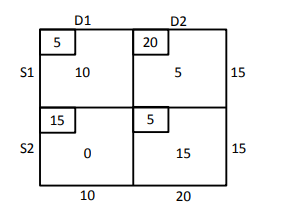
\includegraphics[width=0.75\columnwidth]{chapters/10/7/2/4/figs/fig.png}
 \end{center}
\caption{}
\label{fig:10/7/2/4Fig1}
\end{figure}
\fi

\item Find the position vector of the mid point of the vector joining the points $\vec{P}$(2, 3, 4)
and $\vec{Q}$(4, 1, –2).
\\
\solution
		\begin{enumerate}[label=\thesubsection.\arabic*,ref=\thesubsection.\theenumi]
\item Find the coordinates of the point which divides the join of $(-1,7) $ and $ (4,-3)$ in the ratio 2:3.
	\\
		\solution
	\input{chapters/10/7/2/1/section.tex}
\item Find the coordinates of the point $\vec{R}$ on the line segment joining the points $\vec{P}(-1,3)$ and $\vec{Q}(2,5)$ such that $PR=\frac{3}{5}PQ$.
\item Find the ratio in which the point $\vec{P}\brak{\frac{3}{4},\frac{5}{12}}$ divides the line segment joining the points $\vec{A}\brak{\frac{1}{2},\frac{3}{2}}$ and $ \vec{B}(2,-5)$.
\item Find the coordinates of the point which divides the line segment joining the points $(4,-3)$ and $(8,5)$ in the ratio $3:1$ internally.
\item Find the coordinates of the point $\vec{P}$ on $AD$ such that $AP : PD = 2 : 1$.
\item If the point $\vec{P} (2, 1)$ lies on the line segment joining points $\vec{A} (4, 2)$  and $ \vec{B} (8, 4)$,
then
\begin{enumerate}
	\item $AP =\frac{1}{3}{AB}$ 
\item ${AP}={PE}$
\item ${PB}=\frac{1}{3}{AB}$
\item${AP}=\frac{1}{2}{AB}$
 \end{enumerate}
\item Find the ratio in which the line segment joining the points $(-3,10)$  and  $(6,-8)$  is divided by $ (-1,6)$.
	\\
		\solution
	\input{chapters/10/7/2/4/section.tex}
\item Find the position vector of the mid point of the vector joining the points $\vec{P}$(2, 3, 4)
and $\vec{Q}$(4, 1, –2).
\\
\solution
		\input{chapters/12/10/2/16/section.tex}
\item Let $\vec{A}(4, 2), \vec{B}(6, 5)$  and $ \vec{C}(1, 4)$ be the vertices of $\triangle ABC$.
\begin{enumerate}
\item If $\vec{A}$ and  $\vec{B}$ are $(-2,-2)$ and  $(2,-4)$, respectively, find the coordinates of $\vec{P}$ such that $AP= \frac {3}{7}AB$  and $ \vec{P}$ lies on the line segment $AB$.
	\\
		\solution
	\input{chapters/10/7/2/8/section.tex}
\item Find the coordinates of the points which divide the line segment joining $A(-2,2)$  and  $\vec{B}(2,8)$ into four equal parts.
	\\
		\solution
	\input{chapters/10/7/2/9/section.tex}
\item In what ratio does the point $(-4,6)$ divide the line segment joining the points $\vec{A}(-6,0)$ and $\vec{B}(3,-8)$?
\item Given that $\vec{P}(3,2,-4), \vec{Q}(5,4,-6)$ and $\vec{R}(9,8,-10)$ are collinear. Find the ratio in which $\vec{Q}$ divides $PR$.
\item Points $\vec{A}(-6,10),\vec{B}(-4,6)$  and  $\vec{C}(3,-8)$ are collinear such that $AB=  \frac{2}{9}AC$.
\item The point which divides the line segment joining the points $\vec{P} (7, –6) $  and  $\vec{Q}(3, 4)$ in the 
ratio 1 : 2 internally lies in  which quadrant?
\item Find the coordinates of the points of trisection of the line segment joining $(4,-1)$  and  $(-2,3)$.
	\\
		\solution
	\input{chapters/10/7/2/2/section.tex}
\item Find the coordinates of the points which trisect the line segment joining the points $\vec{P}(4,2,-6)$ and $\vec{Q}(10,-16,6)$.
\item Find the coordinates of the points of trisection (i.e. points dividing to three equal parts) of the line segment joining the points $\vec{A}(2,-2)$ and $\vec{B}(-7,4)$.
\item Point $\vec{P}(5,-3)$ is one of the two points of trisection of line segment joining the points $\vec{A}(7,-2)$ and $\vec{B}(1,-5)$
\item Find the position vector of a point $\vec{R}$ which divides the line joining two points $\vec{P}$
and $\vec{Q}$ whose position vectors are $\hat{i}+2\hat{j}-\hat{k}$ and $-\hat{i}+\hat{j}+\hat{k}$ respectively, in the
ratio 2 : 1
\begin{enumerate}
    \item  internally
    \item  externally
\end{enumerate}
%\solution
%		\input{chapters/12/10/2/15/section.tex}
\item Find the coordinates of the point which divides the line segment joining the points which divides the line segment joining  the points $(-2,3,5)$ and $(1,-4,6)$ in the ratio 
\begin{enumerate}
\item $2:3$ internally,
\item $2:3$ externally
\end{enumerate}
\item Find the coordinates of the point which divides the line segment joining the points $(1,-2,3)$ and $(3,4,-5)$ in the ratio $2:3$
\begin{enumerate}
\item internally, and
\item externally
\end{enumerate}
\item Consider two points $\vec{P}$ and $\vec{Q}$ with position vectors $\overrightarrow{OP} = 3\overrightarrow{a}-2\overrightarrow{b}$ and $\overrightarrow{OQ}=\overrightarrow{a}+\overrightarrow{b}$. Find the position vector of a point $\vec{R}$ which divides the line joining $\vec{P}$ and $\vec{Q}$ in the ratio $2:1$, 
\begin{enumerate}
\item internally, and 
\item externally.
\end{enumerate}
\item The median from $\vec{A}$ meets $BC$ at $\vec{D}$. Find the coordinates of the point $\vec{D}$.
\item Find the coordinates of points $\vec{Q}$ and $\vec{R}$ on medians $BE$ and $CF$ respectively such that $BQ : QE = 2 : 1$  and  $CR : RF = 2 : 1$.
\item What do you observe?
\item If $\vec{A}, \vec{B}$ and $\vec{C}$  are the vertices of $\triangle ABC$, find the coordinates of the centroid of the triangle.
\end{enumerate}
\solution
	\input{chapters/10/7/4/7/section.tex}
\item If $\vec{P}(9a-2,-b)$ divides line segment joining $\vec{A}(3a+1,-3)$ and $\vec{B}(8a,5)$ in the ratio 3:1, find the values of $a$ and $b$.
\item Find the position vector of a point $\vec{R}$ which divides the line joining two points $\vec{P}$ and $\vec{Q}$ whose position vectors are $2\vec{a}+\vec{b}$ and $\vec{a}-3\vec{b}$ externally in the ratio $1:2$.
\item The position vector of the point which divides the join of points 2$\vec{a}$-3$\vec{b}$ $\text{and}$ $\vec{a}+\vec{b}$ in the ratio 3:1 is \rule{1cm}{0.1pt}.
\item If $\vec{a}$ and $\vec{b}$ are the postion vectors of $\vec{A}$ and $\vec{B}$, respectively, find the position vector of a point $\vec{C}$ in $BA$ produced such that $BC=1.5BA$.
\item Find the position vector of a point $\vec{R}$ which divides the line joining two points $\vec{P}$ and $\vec{Q}$ whose position vectors are $(2\vec{a}+\vec{b})$ and $(\vec{a}-3\vec{b})$
externally in the ratio 1 : 2. Also, show that $\vec{P}$ is the mid point of the line segment $RQ$.
\end{enumerate}

\item Let $\vec{A}(4, 2), \vec{B}(6, 5)$  and $ \vec{C}(1, 4)$ be the vertices of $\triangle ABC$.
\begin{enumerate}
\item If $\vec{A}$ and  $\vec{B}$ are $(-2,-2)$ and  $(2,-4)$, respectively, find the coordinates of $\vec{P}$ such that $AP= \frac {3}{7}AB$  and $ \vec{P}$ lies on the line segment $AB$.
	\\
		\solution
	\begin{enumerate}[label=\thesubsection.\arabic*,ref=\thesubsection.\theenumi]
\item Find the coordinates of the point which divides the join of $(-1,7) $ and $ (4,-3)$ in the ratio 2:3.
	\\
		\solution
	\input{chapters/10/7/2/1/section.tex}
\item Find the coordinates of the point $\vec{R}$ on the line segment joining the points $\vec{P}(-1,3)$ and $\vec{Q}(2,5)$ such that $PR=\frac{3}{5}PQ$.
\item Find the ratio in which the point $\vec{P}\brak{\frac{3}{4},\frac{5}{12}}$ divides the line segment joining the points $\vec{A}\brak{\frac{1}{2},\frac{3}{2}}$ and $ \vec{B}(2,-5)$.
\item Find the coordinates of the point which divides the line segment joining the points $(4,-3)$ and $(8,5)$ in the ratio $3:1$ internally.
\item Find the coordinates of the point $\vec{P}$ on $AD$ such that $AP : PD = 2 : 1$.
\item If the point $\vec{P} (2, 1)$ lies on the line segment joining points $\vec{A} (4, 2)$  and $ \vec{B} (8, 4)$,
then
\begin{enumerate}
	\item $AP =\frac{1}{3}{AB}$ 
\item ${AP}={PE}$
\item ${PB}=\frac{1}{3}{AB}$
\item${AP}=\frac{1}{2}{AB}$
 \end{enumerate}
\item Find the ratio in which the line segment joining the points $(-3,10)$  and  $(6,-8)$  is divided by $ (-1,6)$.
	\\
		\solution
	\input{chapters/10/7/2/4/section.tex}
\item Find the position vector of the mid point of the vector joining the points $\vec{P}$(2, 3, 4)
and $\vec{Q}$(4, 1, –2).
\\
\solution
		\input{chapters/12/10/2/16/section.tex}
\item Let $\vec{A}(4, 2), \vec{B}(6, 5)$  and $ \vec{C}(1, 4)$ be the vertices of $\triangle ABC$.
\begin{enumerate}
\item If $\vec{A}$ and  $\vec{B}$ are $(-2,-2)$ and  $(2,-4)$, respectively, find the coordinates of $\vec{P}$ such that $AP= \frac {3}{7}AB$  and $ \vec{P}$ lies on the line segment $AB$.
	\\
		\solution
	\input{chapters/10/7/2/8/section.tex}
\item Find the coordinates of the points which divide the line segment joining $A(-2,2)$  and  $\vec{B}(2,8)$ into four equal parts.
	\\
		\solution
	\input{chapters/10/7/2/9/section.tex}
\item In what ratio does the point $(-4,6)$ divide the line segment joining the points $\vec{A}(-6,0)$ and $\vec{B}(3,-8)$?
\item Given that $\vec{P}(3,2,-4), \vec{Q}(5,4,-6)$ and $\vec{R}(9,8,-10)$ are collinear. Find the ratio in which $\vec{Q}$ divides $PR$.
\item Points $\vec{A}(-6,10),\vec{B}(-4,6)$  and  $\vec{C}(3,-8)$ are collinear such that $AB=  \frac{2}{9}AC$.
\item The point which divides the line segment joining the points $\vec{P} (7, –6) $  and  $\vec{Q}(3, 4)$ in the 
ratio 1 : 2 internally lies in  which quadrant?
\item Find the coordinates of the points of trisection of the line segment joining $(4,-1)$  and  $(-2,3)$.
	\\
		\solution
	\input{chapters/10/7/2/2/section.tex}
\item Find the coordinates of the points which trisect the line segment joining the points $\vec{P}(4,2,-6)$ and $\vec{Q}(10,-16,6)$.
\item Find the coordinates of the points of trisection (i.e. points dividing to three equal parts) of the line segment joining the points $\vec{A}(2,-2)$ and $\vec{B}(-7,4)$.
\item Point $\vec{P}(5,-3)$ is one of the two points of trisection of line segment joining the points $\vec{A}(7,-2)$ and $\vec{B}(1,-5)$
\item Find the position vector of a point $\vec{R}$ which divides the line joining two points $\vec{P}$
and $\vec{Q}$ whose position vectors are $\hat{i}+2\hat{j}-\hat{k}$ and $-\hat{i}+\hat{j}+\hat{k}$ respectively, in the
ratio 2 : 1
\begin{enumerate}
    \item  internally
    \item  externally
\end{enumerate}
%\solution
%		\input{chapters/12/10/2/15/section.tex}
\item Find the coordinates of the point which divides the line segment joining the points which divides the line segment joining  the points $(-2,3,5)$ and $(1,-4,6)$ in the ratio 
\begin{enumerate}
\item $2:3$ internally,
\item $2:3$ externally
\end{enumerate}
\item Find the coordinates of the point which divides the line segment joining the points $(1,-2,3)$ and $(3,4,-5)$ in the ratio $2:3$
\begin{enumerate}
\item internally, and
\item externally
\end{enumerate}
\item Consider two points $\vec{P}$ and $\vec{Q}$ with position vectors $\overrightarrow{OP} = 3\overrightarrow{a}-2\overrightarrow{b}$ and $\overrightarrow{OQ}=\overrightarrow{a}+\overrightarrow{b}$. Find the position vector of a point $\vec{R}$ which divides the line joining $\vec{P}$ and $\vec{Q}$ in the ratio $2:1$, 
\begin{enumerate}
\item internally, and 
\item externally.
\end{enumerate}
\item The median from $\vec{A}$ meets $BC$ at $\vec{D}$. Find the coordinates of the point $\vec{D}$.
\item Find the coordinates of points $\vec{Q}$ and $\vec{R}$ on medians $BE$ and $CF$ respectively such that $BQ : QE = 2 : 1$  and  $CR : RF = 2 : 1$.
\item What do you observe?
\item If $\vec{A}, \vec{B}$ and $\vec{C}$  are the vertices of $\triangle ABC$, find the coordinates of the centroid of the triangle.
\end{enumerate}
\solution
	\input{chapters/10/7/4/7/section.tex}
\item If $\vec{P}(9a-2,-b)$ divides line segment joining $\vec{A}(3a+1,-3)$ and $\vec{B}(8a,5)$ in the ratio 3:1, find the values of $a$ and $b$.
\item Find the position vector of a point $\vec{R}$ which divides the line joining two points $\vec{P}$ and $\vec{Q}$ whose position vectors are $2\vec{a}+\vec{b}$ and $\vec{a}-3\vec{b}$ externally in the ratio $1:2$.
\item The position vector of the point which divides the join of points 2$\vec{a}$-3$\vec{b}$ $\text{and}$ $\vec{a}+\vec{b}$ in the ratio 3:1 is \rule{1cm}{0.1pt}.
\item If $\vec{a}$ and $\vec{b}$ are the postion vectors of $\vec{A}$ and $\vec{B}$, respectively, find the position vector of a point $\vec{C}$ in $BA$ produced such that $BC=1.5BA$.
\item Find the position vector of a point $\vec{R}$ which divides the line joining two points $\vec{P}$ and $\vec{Q}$ whose position vectors are $(2\vec{a}+\vec{b})$ and $(\vec{a}-3\vec{b})$
externally in the ratio 1 : 2. Also, show that $\vec{P}$ is the mid point of the line segment $RQ$.
\end{enumerate}

\item Find the coordinates of the points which divide the line segment joining $A(-2,2)$  and  $\vec{B}(2,8)$ into four equal parts.
	\\
		\solution
	\begin{enumerate}[label=\thesubsection.\arabic*,ref=\thesubsection.\theenumi]
\item Find the coordinates of the point which divides the join of $(-1,7) $ and $ (4,-3)$ in the ratio 2:3.
	\\
		\solution
	\input{chapters/10/7/2/1/section.tex}
\item Find the coordinates of the point $\vec{R}$ on the line segment joining the points $\vec{P}(-1,3)$ and $\vec{Q}(2,5)$ such that $PR=\frac{3}{5}PQ$.
\item Find the ratio in which the point $\vec{P}\brak{\frac{3}{4},\frac{5}{12}}$ divides the line segment joining the points $\vec{A}\brak{\frac{1}{2},\frac{3}{2}}$ and $ \vec{B}(2,-5)$.
\item Find the coordinates of the point which divides the line segment joining the points $(4,-3)$ and $(8,5)$ in the ratio $3:1$ internally.
\item Find the coordinates of the point $\vec{P}$ on $AD$ such that $AP : PD = 2 : 1$.
\item If the point $\vec{P} (2, 1)$ lies on the line segment joining points $\vec{A} (4, 2)$  and $ \vec{B} (8, 4)$,
then
\begin{enumerate}
	\item $AP =\frac{1}{3}{AB}$ 
\item ${AP}={PE}$
\item ${PB}=\frac{1}{3}{AB}$
\item${AP}=\frac{1}{2}{AB}$
 \end{enumerate}
\item Find the ratio in which the line segment joining the points $(-3,10)$  and  $(6,-8)$  is divided by $ (-1,6)$.
	\\
		\solution
	\input{chapters/10/7/2/4/section.tex}
\item Find the position vector of the mid point of the vector joining the points $\vec{P}$(2, 3, 4)
and $\vec{Q}$(4, 1, –2).
\\
\solution
		\input{chapters/12/10/2/16/section.tex}
\item Let $\vec{A}(4, 2), \vec{B}(6, 5)$  and $ \vec{C}(1, 4)$ be the vertices of $\triangle ABC$.
\begin{enumerate}
\item If $\vec{A}$ and  $\vec{B}$ are $(-2,-2)$ and  $(2,-4)$, respectively, find the coordinates of $\vec{P}$ such that $AP= \frac {3}{7}AB$  and $ \vec{P}$ lies on the line segment $AB$.
	\\
		\solution
	\input{chapters/10/7/2/8/section.tex}
\item Find the coordinates of the points which divide the line segment joining $A(-2,2)$  and  $\vec{B}(2,8)$ into four equal parts.
	\\
		\solution
	\input{chapters/10/7/2/9/section.tex}
\item In what ratio does the point $(-4,6)$ divide the line segment joining the points $\vec{A}(-6,0)$ and $\vec{B}(3,-8)$?
\item Given that $\vec{P}(3,2,-4), \vec{Q}(5,4,-6)$ and $\vec{R}(9,8,-10)$ are collinear. Find the ratio in which $\vec{Q}$ divides $PR$.
\item Points $\vec{A}(-6,10),\vec{B}(-4,6)$  and  $\vec{C}(3,-8)$ are collinear such that $AB=  \frac{2}{9}AC$.
\item The point which divides the line segment joining the points $\vec{P} (7, –6) $  and  $\vec{Q}(3, 4)$ in the 
ratio 1 : 2 internally lies in  which quadrant?
\item Find the coordinates of the points of trisection of the line segment joining $(4,-1)$  and  $(-2,3)$.
	\\
		\solution
	\input{chapters/10/7/2/2/section.tex}
\item Find the coordinates of the points which trisect the line segment joining the points $\vec{P}(4,2,-6)$ and $\vec{Q}(10,-16,6)$.
\item Find the coordinates of the points of trisection (i.e. points dividing to three equal parts) of the line segment joining the points $\vec{A}(2,-2)$ and $\vec{B}(-7,4)$.
\item Point $\vec{P}(5,-3)$ is one of the two points of trisection of line segment joining the points $\vec{A}(7,-2)$ and $\vec{B}(1,-5)$
\item Find the position vector of a point $\vec{R}$ which divides the line joining two points $\vec{P}$
and $\vec{Q}$ whose position vectors are $\hat{i}+2\hat{j}-\hat{k}$ and $-\hat{i}+\hat{j}+\hat{k}$ respectively, in the
ratio 2 : 1
\begin{enumerate}
    \item  internally
    \item  externally
\end{enumerate}
%\solution
%		\input{chapters/12/10/2/15/section.tex}
\item Find the coordinates of the point which divides the line segment joining the points which divides the line segment joining  the points $(-2,3,5)$ and $(1,-4,6)$ in the ratio 
\begin{enumerate}
\item $2:3$ internally,
\item $2:3$ externally
\end{enumerate}
\item Find the coordinates of the point which divides the line segment joining the points $(1,-2,3)$ and $(3,4,-5)$ in the ratio $2:3$
\begin{enumerate}
\item internally, and
\item externally
\end{enumerate}
\item Consider two points $\vec{P}$ and $\vec{Q}$ with position vectors $\overrightarrow{OP} = 3\overrightarrow{a}-2\overrightarrow{b}$ and $\overrightarrow{OQ}=\overrightarrow{a}+\overrightarrow{b}$. Find the position vector of a point $\vec{R}$ which divides the line joining $\vec{P}$ and $\vec{Q}$ in the ratio $2:1$, 
\begin{enumerate}
\item internally, and 
\item externally.
\end{enumerate}
\item The median from $\vec{A}$ meets $BC$ at $\vec{D}$. Find the coordinates of the point $\vec{D}$.
\item Find the coordinates of points $\vec{Q}$ and $\vec{R}$ on medians $BE$ and $CF$ respectively such that $BQ : QE = 2 : 1$  and  $CR : RF = 2 : 1$.
\item What do you observe?
\item If $\vec{A}, \vec{B}$ and $\vec{C}$  are the vertices of $\triangle ABC$, find the coordinates of the centroid of the triangle.
\end{enumerate}
\solution
	\input{chapters/10/7/4/7/section.tex}
\item If $\vec{P}(9a-2,-b)$ divides line segment joining $\vec{A}(3a+1,-3)$ and $\vec{B}(8a,5)$ in the ratio 3:1, find the values of $a$ and $b$.
\item Find the position vector of a point $\vec{R}$ which divides the line joining two points $\vec{P}$ and $\vec{Q}$ whose position vectors are $2\vec{a}+\vec{b}$ and $\vec{a}-3\vec{b}$ externally in the ratio $1:2$.
\item The position vector of the point which divides the join of points 2$\vec{a}$-3$\vec{b}$ $\text{and}$ $\vec{a}+\vec{b}$ in the ratio 3:1 is \rule{1cm}{0.1pt}.
\item If $\vec{a}$ and $\vec{b}$ are the postion vectors of $\vec{A}$ and $\vec{B}$, respectively, find the position vector of a point $\vec{C}$ in $BA$ produced such that $BC=1.5BA$.
\item Find the position vector of a point $\vec{R}$ which divides the line joining two points $\vec{P}$ and $\vec{Q}$ whose position vectors are $(2\vec{a}+\vec{b})$ and $(\vec{a}-3\vec{b})$
externally in the ratio 1 : 2. Also, show that $\vec{P}$ is the mid point of the line segment $RQ$.
\end{enumerate}

\item In what ratio does the point $(-4,6)$ divide the line segment joining the points $\vec{A}(-6,0)$ and $\vec{B}(3,-8)$?
\item Given that $\vec{P}(3,2,-4), \vec{Q}(5,4,-6)$ and $\vec{R}(9,8,-10)$ are collinear. Find the ratio in which $\vec{Q}$ divides $PR$.
\item Points $\vec{A}(-6,10),\vec{B}(-4,6)$  and  $\vec{C}(3,-8)$ are collinear such that $AB=  \frac{2}{9}AC$.
\item The point which divides the line segment joining the points $\vec{P} (7, –6) $  and  $\vec{Q}(3, 4)$ in the 
ratio 1 : 2 internally lies in  which quadrant?
\item Find the coordinates of the points of trisection of the line segment joining $(4,-1)$  and  $(-2,3)$.
	\\
		\solution
	Using section formula,
\begin{align}
\vec{R}=\frac{1}{1+\frac{1}{2}}\brak{\myvec{4\\-1}+\frac{1}{2}\myvec{-2\\3}}
=\myvec{2\\ \frac{1}{3}}\\
\vec{S}=\frac{1}{1+\frac{2}{1}}\brak{\myvec{4\\-1}+\frac{2}{1}\myvec{-2\\3}}
=\myvec{0\\ \frac{5}{3}}
\end{align}
which are the desired points of trisection.
\iffalse
See
		\figref{fig:chapters/10/7/2/2/Figure}
\begin{figure}[H]
\centering
\includegraphics[width=0.75\columnwidth]{chapters/10/7/2/2/figs/dj.pdf}
\caption{}
		\label{fig:chapters/10/7/2/2/Figure}
\end{figure}
\fi

\item Find the coordinates of the points which trisect the line segment joining the points $\vec{P}(4,2,-6)$ and $\vec{Q}(10,-16,6)$.
\item Find the coordinates of the points of trisection (i.e. points dividing to three equal parts) of the line segment joining the points $\vec{A}(2,-2)$ and $\vec{B}(-7,4)$.
\item Point $\vec{P}(5,-3)$ is one of the two points of trisection of line segment joining the points $\vec{A}(7,-2)$ and $\vec{B}(1,-5)$
\item Find the position vector of a point $\vec{R}$ which divides the line joining two points $\vec{P}$
and $\vec{Q}$ whose position vectors are $\hat{i}+2\hat{j}-\hat{k}$ and $-\hat{i}+\hat{j}+\hat{k}$ respectively, in the
ratio 2 : 1
\begin{enumerate}
    \item  internally
    \item  externally
\end{enumerate}
%\solution
%		\begin{enumerate}[label=\thesubsection.\arabic*,ref=\thesubsection.\theenumi]
\item Find the coordinates of the point which divides the join of $(-1,7) $ and $ (4,-3)$ in the ratio 2:3.
	\\
		\solution
	\input{chapters/10/7/2/1/section.tex}
\item Find the coordinates of the point $\vec{R}$ on the line segment joining the points $\vec{P}(-1,3)$ and $\vec{Q}(2,5)$ such that $PR=\frac{3}{5}PQ$.
\item Find the ratio in which the point $\vec{P}\brak{\frac{3}{4},\frac{5}{12}}$ divides the line segment joining the points $\vec{A}\brak{\frac{1}{2},\frac{3}{2}}$ and $ \vec{B}(2,-5)$.
\item Find the coordinates of the point which divides the line segment joining the points $(4,-3)$ and $(8,5)$ in the ratio $3:1$ internally.
\item Find the coordinates of the point $\vec{P}$ on $AD$ such that $AP : PD = 2 : 1$.
\item If the point $\vec{P} (2, 1)$ lies on the line segment joining points $\vec{A} (4, 2)$  and $ \vec{B} (8, 4)$,
then
\begin{enumerate}
	\item $AP =\frac{1}{3}{AB}$ 
\item ${AP}={PE}$
\item ${PB}=\frac{1}{3}{AB}$
\item${AP}=\frac{1}{2}{AB}$
 \end{enumerate}
\item Find the ratio in which the line segment joining the points $(-3,10)$  and  $(6,-8)$  is divided by $ (-1,6)$.
	\\
		\solution
	\input{chapters/10/7/2/4/section.tex}
\item Find the position vector of the mid point of the vector joining the points $\vec{P}$(2, 3, 4)
and $\vec{Q}$(4, 1, –2).
\\
\solution
		\input{chapters/12/10/2/16/section.tex}
\item Let $\vec{A}(4, 2), \vec{B}(6, 5)$  and $ \vec{C}(1, 4)$ be the vertices of $\triangle ABC$.
\begin{enumerate}
\item If $\vec{A}$ and  $\vec{B}$ are $(-2,-2)$ and  $(2,-4)$, respectively, find the coordinates of $\vec{P}$ such that $AP= \frac {3}{7}AB$  and $ \vec{P}$ lies on the line segment $AB$.
	\\
		\solution
	\input{chapters/10/7/2/8/section.tex}
\item Find the coordinates of the points which divide the line segment joining $A(-2,2)$  and  $\vec{B}(2,8)$ into four equal parts.
	\\
		\solution
	\input{chapters/10/7/2/9/section.tex}
\item In what ratio does the point $(-4,6)$ divide the line segment joining the points $\vec{A}(-6,0)$ and $\vec{B}(3,-8)$?
\item Given that $\vec{P}(3,2,-4), \vec{Q}(5,4,-6)$ and $\vec{R}(9,8,-10)$ are collinear. Find the ratio in which $\vec{Q}$ divides $PR$.
\item Points $\vec{A}(-6,10),\vec{B}(-4,6)$  and  $\vec{C}(3,-8)$ are collinear such that $AB=  \frac{2}{9}AC$.
\item The point which divides the line segment joining the points $\vec{P} (7, –6) $  and  $\vec{Q}(3, 4)$ in the 
ratio 1 : 2 internally lies in  which quadrant?
\item Find the coordinates of the points of trisection of the line segment joining $(4,-1)$  and  $(-2,3)$.
	\\
		\solution
	\input{chapters/10/7/2/2/section.tex}
\item Find the coordinates of the points which trisect the line segment joining the points $\vec{P}(4,2,-6)$ and $\vec{Q}(10,-16,6)$.
\item Find the coordinates of the points of trisection (i.e. points dividing to three equal parts) of the line segment joining the points $\vec{A}(2,-2)$ and $\vec{B}(-7,4)$.
\item Point $\vec{P}(5,-3)$ is one of the two points of trisection of line segment joining the points $\vec{A}(7,-2)$ and $\vec{B}(1,-5)$
\item Find the position vector of a point $\vec{R}$ which divides the line joining two points $\vec{P}$
and $\vec{Q}$ whose position vectors are $\hat{i}+2\hat{j}-\hat{k}$ and $-\hat{i}+\hat{j}+\hat{k}$ respectively, in the
ratio 2 : 1
\begin{enumerate}
    \item  internally
    \item  externally
\end{enumerate}
%\solution
%		\input{chapters/12/10/2/15/section.tex}
\item Find the coordinates of the point which divides the line segment joining the points which divides the line segment joining  the points $(-2,3,5)$ and $(1,-4,6)$ in the ratio 
\begin{enumerate}
\item $2:3$ internally,
\item $2:3$ externally
\end{enumerate}
\item Find the coordinates of the point which divides the line segment joining the points $(1,-2,3)$ and $(3,4,-5)$ in the ratio $2:3$
\begin{enumerate}
\item internally, and
\item externally
\end{enumerate}
\item Consider two points $\vec{P}$ and $\vec{Q}$ with position vectors $\overrightarrow{OP} = 3\overrightarrow{a}-2\overrightarrow{b}$ and $\overrightarrow{OQ}=\overrightarrow{a}+\overrightarrow{b}$. Find the position vector of a point $\vec{R}$ which divides the line joining $\vec{P}$ and $\vec{Q}$ in the ratio $2:1$, 
\begin{enumerate}
\item internally, and 
\item externally.
\end{enumerate}
\item The median from $\vec{A}$ meets $BC$ at $\vec{D}$. Find the coordinates of the point $\vec{D}$.
\item Find the coordinates of points $\vec{Q}$ and $\vec{R}$ on medians $BE$ and $CF$ respectively such that $BQ : QE = 2 : 1$  and  $CR : RF = 2 : 1$.
\item What do you observe?
\item If $\vec{A}, \vec{B}$ and $\vec{C}$  are the vertices of $\triangle ABC$, find the coordinates of the centroid of the triangle.
\end{enumerate}
\solution
	\input{chapters/10/7/4/7/section.tex}
\item If $\vec{P}(9a-2,-b)$ divides line segment joining $\vec{A}(3a+1,-3)$ and $\vec{B}(8a,5)$ in the ratio 3:1, find the values of $a$ and $b$.
\item Find the position vector of a point $\vec{R}$ which divides the line joining two points $\vec{P}$ and $\vec{Q}$ whose position vectors are $2\vec{a}+\vec{b}$ and $\vec{a}-3\vec{b}$ externally in the ratio $1:2$.
\item The position vector of the point which divides the join of points 2$\vec{a}$-3$\vec{b}$ $\text{and}$ $\vec{a}+\vec{b}$ in the ratio 3:1 is \rule{1cm}{0.1pt}.
\item If $\vec{a}$ and $\vec{b}$ are the postion vectors of $\vec{A}$ and $\vec{B}$, respectively, find the position vector of a point $\vec{C}$ in $BA$ produced such that $BC=1.5BA$.
\item Find the position vector of a point $\vec{R}$ which divides the line joining two points $\vec{P}$ and $\vec{Q}$ whose position vectors are $(2\vec{a}+\vec{b})$ and $(\vec{a}-3\vec{b})$
externally in the ratio 1 : 2. Also, show that $\vec{P}$ is the mid point of the line segment $RQ$.
\end{enumerate}

\item Find the coordinates of the point which divides the line segment joining the points which divides the line segment joining  the points $(-2,3,5)$ and $(1,-4,6)$ in the ratio 
\begin{enumerate}
\item $2:3$ internally,
\item $2:3$ externally
\end{enumerate}
\item Find the coordinates of the point which divides the line segment joining the points $(1,-2,3)$ and $(3,4,-5)$ in the ratio $2:3$
\begin{enumerate}
\item internally, and
\item externally
\end{enumerate}
\item Consider two points $\vec{P}$ and $\vec{Q}$ with position vectors $\overrightarrow{OP} = 3\overrightarrow{a}-2\overrightarrow{b}$ and $\overrightarrow{OQ}=\overrightarrow{a}+\overrightarrow{b}$. Find the position vector of a point $\vec{R}$ which divides the line joining $\vec{P}$ and $\vec{Q}$ in the ratio $2:1$, 
\begin{enumerate}
\item internally, and 
\item externally.
\end{enumerate}
\item The median from $\vec{A}$ meets $BC$ at $\vec{D}$. Find the coordinates of the point $\vec{D}$.
\item Find the coordinates of points $\vec{Q}$ and $\vec{R}$ on medians $BE$ and $CF$ respectively such that $BQ : QE = 2 : 1$  and  $CR : RF = 2 : 1$.
\item What do you observe?
\item If $\vec{A}, \vec{B}$ and $\vec{C}$  are the vertices of $\triangle ABC$, find the coordinates of the centroid of the triangle.
\end{enumerate}
\solution
	\begin{enumerate}[label=\thesubsection.\arabic*,ref=\thesubsection.\theenumi]
\item Find the coordinates of the point which divides the join of $(-1,7) $ and $ (4,-3)$ in the ratio 2:3.
	\\
		\solution
	\input{chapters/10/7/2/1/section.tex}
\item Find the coordinates of the point $\vec{R}$ on the line segment joining the points $\vec{P}(-1,3)$ and $\vec{Q}(2,5)$ such that $PR=\frac{3}{5}PQ$.
\item Find the ratio in which the point $\vec{P}\brak{\frac{3}{4},\frac{5}{12}}$ divides the line segment joining the points $\vec{A}\brak{\frac{1}{2},\frac{3}{2}}$ and $ \vec{B}(2,-5)$.
\item Find the coordinates of the point which divides the line segment joining the points $(4,-3)$ and $(8,5)$ in the ratio $3:1$ internally.
\item Find the coordinates of the point $\vec{P}$ on $AD$ such that $AP : PD = 2 : 1$.
\item If the point $\vec{P} (2, 1)$ lies on the line segment joining points $\vec{A} (4, 2)$  and $ \vec{B} (8, 4)$,
then
\begin{enumerate}
	\item $AP =\frac{1}{3}{AB}$ 
\item ${AP}={PE}$
\item ${PB}=\frac{1}{3}{AB}$
\item${AP}=\frac{1}{2}{AB}$
 \end{enumerate}
\item Find the ratio in which the line segment joining the points $(-3,10)$  and  $(6,-8)$  is divided by $ (-1,6)$.
	\\
		\solution
	\input{chapters/10/7/2/4/section.tex}
\item Find the position vector of the mid point of the vector joining the points $\vec{P}$(2, 3, 4)
and $\vec{Q}$(4, 1, –2).
\\
\solution
		\input{chapters/12/10/2/16/section.tex}
\item Let $\vec{A}(4, 2), \vec{B}(6, 5)$  and $ \vec{C}(1, 4)$ be the vertices of $\triangle ABC$.
\begin{enumerate}
\item If $\vec{A}$ and  $\vec{B}$ are $(-2,-2)$ and  $(2,-4)$, respectively, find the coordinates of $\vec{P}$ such that $AP= \frac {3}{7}AB$  and $ \vec{P}$ lies on the line segment $AB$.
	\\
		\solution
	\input{chapters/10/7/2/8/section.tex}
\item Find the coordinates of the points which divide the line segment joining $A(-2,2)$  and  $\vec{B}(2,8)$ into four equal parts.
	\\
		\solution
	\input{chapters/10/7/2/9/section.tex}
\item In what ratio does the point $(-4,6)$ divide the line segment joining the points $\vec{A}(-6,0)$ and $\vec{B}(3,-8)$?
\item Given that $\vec{P}(3,2,-4), \vec{Q}(5,4,-6)$ and $\vec{R}(9,8,-10)$ are collinear. Find the ratio in which $\vec{Q}$ divides $PR$.
\item Points $\vec{A}(-6,10),\vec{B}(-4,6)$  and  $\vec{C}(3,-8)$ are collinear such that $AB=  \frac{2}{9}AC$.
\item The point which divides the line segment joining the points $\vec{P} (7, –6) $  and  $\vec{Q}(3, 4)$ in the 
ratio 1 : 2 internally lies in  which quadrant?
\item Find the coordinates of the points of trisection of the line segment joining $(4,-1)$  and  $(-2,3)$.
	\\
		\solution
	\input{chapters/10/7/2/2/section.tex}
\item Find the coordinates of the points which trisect the line segment joining the points $\vec{P}(4,2,-6)$ and $\vec{Q}(10,-16,6)$.
\item Find the coordinates of the points of trisection (i.e. points dividing to three equal parts) of the line segment joining the points $\vec{A}(2,-2)$ and $\vec{B}(-7,4)$.
\item Point $\vec{P}(5,-3)$ is one of the two points of trisection of line segment joining the points $\vec{A}(7,-2)$ and $\vec{B}(1,-5)$
\item Find the position vector of a point $\vec{R}$ which divides the line joining two points $\vec{P}$
and $\vec{Q}$ whose position vectors are $\hat{i}+2\hat{j}-\hat{k}$ and $-\hat{i}+\hat{j}+\hat{k}$ respectively, in the
ratio 2 : 1
\begin{enumerate}
    \item  internally
    \item  externally
\end{enumerate}
%\solution
%		\input{chapters/12/10/2/15/section.tex}
\item Find the coordinates of the point which divides the line segment joining the points which divides the line segment joining  the points $(-2,3,5)$ and $(1,-4,6)$ in the ratio 
\begin{enumerate}
\item $2:3$ internally,
\item $2:3$ externally
\end{enumerate}
\item Find the coordinates of the point which divides the line segment joining the points $(1,-2,3)$ and $(3,4,-5)$ in the ratio $2:3$
\begin{enumerate}
\item internally, and
\item externally
\end{enumerate}
\item Consider two points $\vec{P}$ and $\vec{Q}$ with position vectors $\overrightarrow{OP} = 3\overrightarrow{a}-2\overrightarrow{b}$ and $\overrightarrow{OQ}=\overrightarrow{a}+\overrightarrow{b}$. Find the position vector of a point $\vec{R}$ which divides the line joining $\vec{P}$ and $\vec{Q}$ in the ratio $2:1$, 
\begin{enumerate}
\item internally, and 
\item externally.
\end{enumerate}
\item The median from $\vec{A}$ meets $BC$ at $\vec{D}$. Find the coordinates of the point $\vec{D}$.
\item Find the coordinates of points $\vec{Q}$ and $\vec{R}$ on medians $BE$ and $CF$ respectively such that $BQ : QE = 2 : 1$  and  $CR : RF = 2 : 1$.
\item What do you observe?
\item If $\vec{A}, \vec{B}$ and $\vec{C}$  are the vertices of $\triangle ABC$, find the coordinates of the centroid of the triangle.
\end{enumerate}
\solution
	\input{chapters/10/7/4/7/section.tex}
\item If $\vec{P}(9a-2,-b)$ divides line segment joining $\vec{A}(3a+1,-3)$ and $\vec{B}(8a,5)$ in the ratio 3:1, find the values of $a$ and $b$.
\item Find the position vector of a point $\vec{R}$ which divides the line joining two points $\vec{P}$ and $\vec{Q}$ whose position vectors are $2\vec{a}+\vec{b}$ and $\vec{a}-3\vec{b}$ externally in the ratio $1:2$.
\item The position vector of the point which divides the join of points 2$\vec{a}$-3$\vec{b}$ $\text{and}$ $\vec{a}+\vec{b}$ in the ratio 3:1 is \rule{1cm}{0.1pt}.
\item If $\vec{a}$ and $\vec{b}$ are the postion vectors of $\vec{A}$ and $\vec{B}$, respectively, find the position vector of a point $\vec{C}$ in $BA$ produced such that $BC=1.5BA$.
\item Find the position vector of a point $\vec{R}$ which divides the line joining two points $\vec{P}$ and $\vec{Q}$ whose position vectors are $(2\vec{a}+\vec{b})$ and $(\vec{a}-3\vec{b})$
externally in the ratio 1 : 2. Also, show that $\vec{P}$ is the mid point of the line segment $RQ$.
\end{enumerate}

\item If $\vec{P}(9a-2,-b)$ divides line segment joining $\vec{A}(3a+1,-3)$ and $\vec{B}(8a,5)$ in the ratio 3:1, find the values of $a$ and $b$.
\item Find the position vector of a point $\vec{R}$ which divides the line joining two points $\vec{P}$ and $\vec{Q}$ whose position vectors are $2\vec{a}+\vec{b}$ and $\vec{a}-3\vec{b}$ externally in the ratio $1:2$.
\item The position vector of the point which divides the join of points 2$\vec{a}$-3$\vec{b}$ $\text{and}$ $\vec{a}+\vec{b}$ in the ratio 3:1 is \rule{1cm}{0.1pt}.
\item If $\vec{a}$ and $\vec{b}$ are the postion vectors of $\vec{A}$ and $\vec{B}$, respectively, find the position vector of a point $\vec{C}$ in $BA$ produced such that $BC=1.5BA$.
\item Find the position vector of a point $\vec{R}$ which divides the line joining two points $\vec{P}$ and $\vec{Q}$ whose position vectors are $(2\vec{a}+\vec{b})$ and $(\vec{a}-3\vec{b})$
externally in the ratio 1 : 2. Also, show that $\vec{P}$ is the mid point of the line segment $RQ$.
\end{enumerate}

\item Let $\vec{A}(4, 2), \vec{B}(6, 5)$  and $ \vec{C}(1, 4)$ be the vertices of $\triangle ABC$.
\begin{enumerate}
\item If $\vec{A}$ and  $\vec{B}$ are $(-2,-2)$ and  $(2,-4)$, respectively, find the coordinates of $\vec{P}$ such that $AP= \frac {3}{7}AB$  and $ \vec{P}$ lies on the line segment $AB$.
	\\
		\solution
	\begin{enumerate}[label=\thesubsection.\arabic*,ref=\thesubsection.\theenumi]
\item Find the coordinates of the point which divides the join of $(-1,7) $ and $ (4,-3)$ in the ratio 2:3.
	\\
		\solution
	\begin{enumerate}[label=\thesubsection.\arabic*,ref=\thesubsection.\theenumi]
\item Find the coordinates of the point which divides the join of $(-1,7) $ and $ (4,-3)$ in the ratio 2:3.
	\\
		\solution
	\input{chapters/10/7/2/1/section.tex}
\item Find the coordinates of the point $\vec{R}$ on the line segment joining the points $\vec{P}(-1,3)$ and $\vec{Q}(2,5)$ such that $PR=\frac{3}{5}PQ$.
\item Find the ratio in which the point $\vec{P}\brak{\frac{3}{4},\frac{5}{12}}$ divides the line segment joining the points $\vec{A}\brak{\frac{1}{2},\frac{3}{2}}$ and $ \vec{B}(2,-5)$.
\item Find the coordinates of the point which divides the line segment joining the points $(4,-3)$ and $(8,5)$ in the ratio $3:1$ internally.
\item Find the coordinates of the point $\vec{P}$ on $AD$ such that $AP : PD = 2 : 1$.
\item If the point $\vec{P} (2, 1)$ lies on the line segment joining points $\vec{A} (4, 2)$  and $ \vec{B} (8, 4)$,
then
\begin{enumerate}
	\item $AP =\frac{1}{3}{AB}$ 
\item ${AP}={PE}$
\item ${PB}=\frac{1}{3}{AB}$
\item${AP}=\frac{1}{2}{AB}$
 \end{enumerate}
\item Find the ratio in which the line segment joining the points $(-3,10)$  and  $(6,-8)$  is divided by $ (-1,6)$.
	\\
		\solution
	\input{chapters/10/7/2/4/section.tex}
\item Find the position vector of the mid point of the vector joining the points $\vec{P}$(2, 3, 4)
and $\vec{Q}$(4, 1, –2).
\\
\solution
		\input{chapters/12/10/2/16/section.tex}
\item Let $\vec{A}(4, 2), \vec{B}(6, 5)$  and $ \vec{C}(1, 4)$ be the vertices of $\triangle ABC$.
\begin{enumerate}
\item If $\vec{A}$ and  $\vec{B}$ are $(-2,-2)$ and  $(2,-4)$, respectively, find the coordinates of $\vec{P}$ such that $AP= \frac {3}{7}AB$  and $ \vec{P}$ lies on the line segment $AB$.
	\\
		\solution
	\input{chapters/10/7/2/8/section.tex}
\item Find the coordinates of the points which divide the line segment joining $A(-2,2)$  and  $\vec{B}(2,8)$ into four equal parts.
	\\
		\solution
	\input{chapters/10/7/2/9/section.tex}
\item In what ratio does the point $(-4,6)$ divide the line segment joining the points $\vec{A}(-6,0)$ and $\vec{B}(3,-8)$?
\item Given that $\vec{P}(3,2,-4), \vec{Q}(5,4,-6)$ and $\vec{R}(9,8,-10)$ are collinear. Find the ratio in which $\vec{Q}$ divides $PR$.
\item Points $\vec{A}(-6,10),\vec{B}(-4,6)$  and  $\vec{C}(3,-8)$ are collinear such that $AB=  \frac{2}{9}AC$.
\item The point which divides the line segment joining the points $\vec{P} (7, –6) $  and  $\vec{Q}(3, 4)$ in the 
ratio 1 : 2 internally lies in  which quadrant?
\item Find the coordinates of the points of trisection of the line segment joining $(4,-1)$  and  $(-2,3)$.
	\\
		\solution
	\input{chapters/10/7/2/2/section.tex}
\item Find the coordinates of the points which trisect the line segment joining the points $\vec{P}(4,2,-6)$ and $\vec{Q}(10,-16,6)$.
\item Find the coordinates of the points of trisection (i.e. points dividing to three equal parts) of the line segment joining the points $\vec{A}(2,-2)$ and $\vec{B}(-7,4)$.
\item Point $\vec{P}(5,-3)$ is one of the two points of trisection of line segment joining the points $\vec{A}(7,-2)$ and $\vec{B}(1,-5)$
\item Find the position vector of a point $\vec{R}$ which divides the line joining two points $\vec{P}$
and $\vec{Q}$ whose position vectors are $\hat{i}+2\hat{j}-\hat{k}$ and $-\hat{i}+\hat{j}+\hat{k}$ respectively, in the
ratio 2 : 1
\begin{enumerate}
    \item  internally
    \item  externally
\end{enumerate}
%\solution
%		\input{chapters/12/10/2/15/section.tex}
\item Find the coordinates of the point which divides the line segment joining the points which divides the line segment joining  the points $(-2,3,5)$ and $(1,-4,6)$ in the ratio 
\begin{enumerate}
\item $2:3$ internally,
\item $2:3$ externally
\end{enumerate}
\item Find the coordinates of the point which divides the line segment joining the points $(1,-2,3)$ and $(3,4,-5)$ in the ratio $2:3$
\begin{enumerate}
\item internally, and
\item externally
\end{enumerate}
\item Consider two points $\vec{P}$ and $\vec{Q}$ with position vectors $\overrightarrow{OP} = 3\overrightarrow{a}-2\overrightarrow{b}$ and $\overrightarrow{OQ}=\overrightarrow{a}+\overrightarrow{b}$. Find the position vector of a point $\vec{R}$ which divides the line joining $\vec{P}$ and $\vec{Q}$ in the ratio $2:1$, 
\begin{enumerate}
\item internally, and 
\item externally.
\end{enumerate}
\item The median from $\vec{A}$ meets $BC$ at $\vec{D}$. Find the coordinates of the point $\vec{D}$.
\item Find the coordinates of points $\vec{Q}$ and $\vec{R}$ on medians $BE$ and $CF$ respectively such that $BQ : QE = 2 : 1$  and  $CR : RF = 2 : 1$.
\item What do you observe?
\item If $\vec{A}, \vec{B}$ and $\vec{C}$  are the vertices of $\triangle ABC$, find the coordinates of the centroid of the triangle.
\end{enumerate}
\solution
	\input{chapters/10/7/4/7/section.tex}
\item If $\vec{P}(9a-2,-b)$ divides line segment joining $\vec{A}(3a+1,-3)$ and $\vec{B}(8a,5)$ in the ratio 3:1, find the values of $a$ and $b$.
\item Find the position vector of a point $\vec{R}$ which divides the line joining two points $\vec{P}$ and $\vec{Q}$ whose position vectors are $2\vec{a}+\vec{b}$ and $\vec{a}-3\vec{b}$ externally in the ratio $1:2$.
\item The position vector of the point which divides the join of points 2$\vec{a}$-3$\vec{b}$ $\text{and}$ $\vec{a}+\vec{b}$ in the ratio 3:1 is \rule{1cm}{0.1pt}.
\item If $\vec{a}$ and $\vec{b}$ are the postion vectors of $\vec{A}$ and $\vec{B}$, respectively, find the position vector of a point $\vec{C}$ in $BA$ produced such that $BC=1.5BA$.
\item Find the position vector of a point $\vec{R}$ which divides the line joining two points $\vec{P}$ and $\vec{Q}$ whose position vectors are $(2\vec{a}+\vec{b})$ and $(\vec{a}-3\vec{b})$
externally in the ratio 1 : 2. Also, show that $\vec{P}$ is the mid point of the line segment $RQ$.
\end{enumerate}

\item Find the coordinates of the point $\vec{R}$ on the line segment joining the points $\vec{P}(-1,3)$ and $\vec{Q}(2,5)$ such that $PR=\frac{3}{5}PQ$.
\item Find the ratio in which the point $\vec{P}\brak{\frac{3}{4},\frac{5}{12}}$ divides the line segment joining the points $\vec{A}\brak{\frac{1}{2},\frac{3}{2}}$ and $ \vec{B}(2,-5)$.
\item Find the coordinates of the point which divides the line segment joining the points $(4,-3)$ and $(8,5)$ in the ratio $3:1$ internally.
\item Find the coordinates of the point $\vec{P}$ on $AD$ such that $AP : PD = 2 : 1$.
\item If the point $\vec{P} (2, 1)$ lies on the line segment joining points $\vec{A} (4, 2)$  and $ \vec{B} (8, 4)$,
then
\begin{enumerate}
	\item $AP =\frac{1}{3}{AB}$ 
\item ${AP}={PE}$
\item ${PB}=\frac{1}{3}{AB}$
\item${AP}=\frac{1}{2}{AB}$
 \end{enumerate}
\item Find the ratio in which the line segment joining the points $(-3,10)$  and  $(6,-8)$  is divided by $ (-1,6)$.
	\\
		\solution
	\iffalse
Using section formula,
\begin{align}
         \myvec{-1\\6} &=\frac{{\myvec{-3\\10}+k\myvec{6\\-8}}}{1+k}\\
	 \implies 7k\myvec{1 \\ -2} &= 2\myvec{1 \\ -2}
	 \\
	 \text{or, } k &= \frac{2}{7}.
\end{align}
\fi
In 
			\eqref{eq:section_formula-k}, substituting
			\begin{align}
				\vec{B} &= \myvec{-3\\10}, \vec{C} = \myvec{6\\-8}, \vec{D} = \myvec{-1\\6},
				\\
				k &= \frac{\myvec{-2 & 4}\myvec{-7 \\ 14}}{\norm{\myvec{-7 \\ 14}}^2} = \frac{2}{7}
			\end{align}
\iffalse
See \figref{fig:10/7/2/4Fig1}.
\begin{figure}[H]
 \begin{center}
  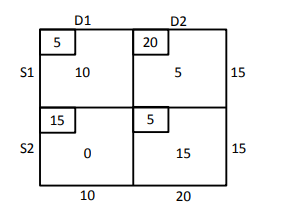
\includegraphics[width=0.75\columnwidth]{chapters/10/7/2/4/figs/fig.png}
 \end{center}
\caption{}
\label{fig:10/7/2/4Fig1}
\end{figure}
\fi

\item Find the position vector of the mid point of the vector joining the points $\vec{P}$(2, 3, 4)
and $\vec{Q}$(4, 1, –2).
\\
\solution
		\begin{enumerate}[label=\thesubsection.\arabic*,ref=\thesubsection.\theenumi]
\item Find the coordinates of the point which divides the join of $(-1,7) $ and $ (4,-3)$ in the ratio 2:3.
	\\
		\solution
	\input{chapters/10/7/2/1/section.tex}
\item Find the coordinates of the point $\vec{R}$ on the line segment joining the points $\vec{P}(-1,3)$ and $\vec{Q}(2,5)$ such that $PR=\frac{3}{5}PQ$.
\item Find the ratio in which the point $\vec{P}\brak{\frac{3}{4},\frac{5}{12}}$ divides the line segment joining the points $\vec{A}\brak{\frac{1}{2},\frac{3}{2}}$ and $ \vec{B}(2,-5)$.
\item Find the coordinates of the point which divides the line segment joining the points $(4,-3)$ and $(8,5)$ in the ratio $3:1$ internally.
\item Find the coordinates of the point $\vec{P}$ on $AD$ such that $AP : PD = 2 : 1$.
\item If the point $\vec{P} (2, 1)$ lies on the line segment joining points $\vec{A} (4, 2)$  and $ \vec{B} (8, 4)$,
then
\begin{enumerate}
	\item $AP =\frac{1}{3}{AB}$ 
\item ${AP}={PE}$
\item ${PB}=\frac{1}{3}{AB}$
\item${AP}=\frac{1}{2}{AB}$
 \end{enumerate}
\item Find the ratio in which the line segment joining the points $(-3,10)$  and  $(6,-8)$  is divided by $ (-1,6)$.
	\\
		\solution
	\input{chapters/10/7/2/4/section.tex}
\item Find the position vector of the mid point of the vector joining the points $\vec{P}$(2, 3, 4)
and $\vec{Q}$(4, 1, –2).
\\
\solution
		\input{chapters/12/10/2/16/section.tex}
\item Let $\vec{A}(4, 2), \vec{B}(6, 5)$  and $ \vec{C}(1, 4)$ be the vertices of $\triangle ABC$.
\begin{enumerate}
\item If $\vec{A}$ and  $\vec{B}$ are $(-2,-2)$ and  $(2,-4)$, respectively, find the coordinates of $\vec{P}$ such that $AP= \frac {3}{7}AB$  and $ \vec{P}$ lies on the line segment $AB$.
	\\
		\solution
	\input{chapters/10/7/2/8/section.tex}
\item Find the coordinates of the points which divide the line segment joining $A(-2,2)$  and  $\vec{B}(2,8)$ into four equal parts.
	\\
		\solution
	\input{chapters/10/7/2/9/section.tex}
\item In what ratio does the point $(-4,6)$ divide the line segment joining the points $\vec{A}(-6,0)$ and $\vec{B}(3,-8)$?
\item Given that $\vec{P}(3,2,-4), \vec{Q}(5,4,-6)$ and $\vec{R}(9,8,-10)$ are collinear. Find the ratio in which $\vec{Q}$ divides $PR$.
\item Points $\vec{A}(-6,10),\vec{B}(-4,6)$  and  $\vec{C}(3,-8)$ are collinear such that $AB=  \frac{2}{9}AC$.
\item The point which divides the line segment joining the points $\vec{P} (7, –6) $  and  $\vec{Q}(3, 4)$ in the 
ratio 1 : 2 internally lies in  which quadrant?
\item Find the coordinates of the points of trisection of the line segment joining $(4,-1)$  and  $(-2,3)$.
	\\
		\solution
	\input{chapters/10/7/2/2/section.tex}
\item Find the coordinates of the points which trisect the line segment joining the points $\vec{P}(4,2,-6)$ and $\vec{Q}(10,-16,6)$.
\item Find the coordinates of the points of trisection (i.e. points dividing to three equal parts) of the line segment joining the points $\vec{A}(2,-2)$ and $\vec{B}(-7,4)$.
\item Point $\vec{P}(5,-3)$ is one of the two points of trisection of line segment joining the points $\vec{A}(7,-2)$ and $\vec{B}(1,-5)$
\item Find the position vector of a point $\vec{R}$ which divides the line joining two points $\vec{P}$
and $\vec{Q}$ whose position vectors are $\hat{i}+2\hat{j}-\hat{k}$ and $-\hat{i}+\hat{j}+\hat{k}$ respectively, in the
ratio 2 : 1
\begin{enumerate}
    \item  internally
    \item  externally
\end{enumerate}
%\solution
%		\input{chapters/12/10/2/15/section.tex}
\item Find the coordinates of the point which divides the line segment joining the points which divides the line segment joining  the points $(-2,3,5)$ and $(1,-4,6)$ in the ratio 
\begin{enumerate}
\item $2:3$ internally,
\item $2:3$ externally
\end{enumerate}
\item Find the coordinates of the point which divides the line segment joining the points $(1,-2,3)$ and $(3,4,-5)$ in the ratio $2:3$
\begin{enumerate}
\item internally, and
\item externally
\end{enumerate}
\item Consider two points $\vec{P}$ and $\vec{Q}$ with position vectors $\overrightarrow{OP} = 3\overrightarrow{a}-2\overrightarrow{b}$ and $\overrightarrow{OQ}=\overrightarrow{a}+\overrightarrow{b}$. Find the position vector of a point $\vec{R}$ which divides the line joining $\vec{P}$ and $\vec{Q}$ in the ratio $2:1$, 
\begin{enumerate}
\item internally, and 
\item externally.
\end{enumerate}
\item The median from $\vec{A}$ meets $BC$ at $\vec{D}$. Find the coordinates of the point $\vec{D}$.
\item Find the coordinates of points $\vec{Q}$ and $\vec{R}$ on medians $BE$ and $CF$ respectively such that $BQ : QE = 2 : 1$  and  $CR : RF = 2 : 1$.
\item What do you observe?
\item If $\vec{A}, \vec{B}$ and $\vec{C}$  are the vertices of $\triangle ABC$, find the coordinates of the centroid of the triangle.
\end{enumerate}
\solution
	\input{chapters/10/7/4/7/section.tex}
\item If $\vec{P}(9a-2,-b)$ divides line segment joining $\vec{A}(3a+1,-3)$ and $\vec{B}(8a,5)$ in the ratio 3:1, find the values of $a$ and $b$.
\item Find the position vector of a point $\vec{R}$ which divides the line joining two points $\vec{P}$ and $\vec{Q}$ whose position vectors are $2\vec{a}+\vec{b}$ and $\vec{a}-3\vec{b}$ externally in the ratio $1:2$.
\item The position vector of the point which divides the join of points 2$\vec{a}$-3$\vec{b}$ $\text{and}$ $\vec{a}+\vec{b}$ in the ratio 3:1 is \rule{1cm}{0.1pt}.
\item If $\vec{a}$ and $\vec{b}$ are the postion vectors of $\vec{A}$ and $\vec{B}$, respectively, find the position vector of a point $\vec{C}$ in $BA$ produced such that $BC=1.5BA$.
\item Find the position vector of a point $\vec{R}$ which divides the line joining two points $\vec{P}$ and $\vec{Q}$ whose position vectors are $(2\vec{a}+\vec{b})$ and $(\vec{a}-3\vec{b})$
externally in the ratio 1 : 2. Also, show that $\vec{P}$ is the mid point of the line segment $RQ$.
\end{enumerate}

\item Let $\vec{A}(4, 2), \vec{B}(6, 5)$  and $ \vec{C}(1, 4)$ be the vertices of $\triangle ABC$.
\begin{enumerate}
\item If $\vec{A}$ and  $\vec{B}$ are $(-2,-2)$ and  $(2,-4)$, respectively, find the coordinates of $\vec{P}$ such that $AP= \frac {3}{7}AB$  and $ \vec{P}$ lies on the line segment $AB$.
	\\
		\solution
	\begin{enumerate}[label=\thesubsection.\arabic*,ref=\thesubsection.\theenumi]
\item Find the coordinates of the point which divides the join of $(-1,7) $ and $ (4,-3)$ in the ratio 2:3.
	\\
		\solution
	\input{chapters/10/7/2/1/section.tex}
\item Find the coordinates of the point $\vec{R}$ on the line segment joining the points $\vec{P}(-1,3)$ and $\vec{Q}(2,5)$ such that $PR=\frac{3}{5}PQ$.
\item Find the ratio in which the point $\vec{P}\brak{\frac{3}{4},\frac{5}{12}}$ divides the line segment joining the points $\vec{A}\brak{\frac{1}{2},\frac{3}{2}}$ and $ \vec{B}(2,-5)$.
\item Find the coordinates of the point which divides the line segment joining the points $(4,-3)$ and $(8,5)$ in the ratio $3:1$ internally.
\item Find the coordinates of the point $\vec{P}$ on $AD$ such that $AP : PD = 2 : 1$.
\item If the point $\vec{P} (2, 1)$ lies on the line segment joining points $\vec{A} (4, 2)$  and $ \vec{B} (8, 4)$,
then
\begin{enumerate}
	\item $AP =\frac{1}{3}{AB}$ 
\item ${AP}={PE}$
\item ${PB}=\frac{1}{3}{AB}$
\item${AP}=\frac{1}{2}{AB}$
 \end{enumerate}
\item Find the ratio in which the line segment joining the points $(-3,10)$  and  $(6,-8)$  is divided by $ (-1,6)$.
	\\
		\solution
	\input{chapters/10/7/2/4/section.tex}
\item Find the position vector of the mid point of the vector joining the points $\vec{P}$(2, 3, 4)
and $\vec{Q}$(4, 1, –2).
\\
\solution
		\input{chapters/12/10/2/16/section.tex}
\item Let $\vec{A}(4, 2), \vec{B}(6, 5)$  and $ \vec{C}(1, 4)$ be the vertices of $\triangle ABC$.
\begin{enumerate}
\item If $\vec{A}$ and  $\vec{B}$ are $(-2,-2)$ and  $(2,-4)$, respectively, find the coordinates of $\vec{P}$ such that $AP= \frac {3}{7}AB$  and $ \vec{P}$ lies on the line segment $AB$.
	\\
		\solution
	\input{chapters/10/7/2/8/section.tex}
\item Find the coordinates of the points which divide the line segment joining $A(-2,2)$  and  $\vec{B}(2,8)$ into four equal parts.
	\\
		\solution
	\input{chapters/10/7/2/9/section.tex}
\item In what ratio does the point $(-4,6)$ divide the line segment joining the points $\vec{A}(-6,0)$ and $\vec{B}(3,-8)$?
\item Given that $\vec{P}(3,2,-4), \vec{Q}(5,4,-6)$ and $\vec{R}(9,8,-10)$ are collinear. Find the ratio in which $\vec{Q}$ divides $PR$.
\item Points $\vec{A}(-6,10),\vec{B}(-4,6)$  and  $\vec{C}(3,-8)$ are collinear such that $AB=  \frac{2}{9}AC$.
\item The point which divides the line segment joining the points $\vec{P} (7, –6) $  and  $\vec{Q}(3, 4)$ in the 
ratio 1 : 2 internally lies in  which quadrant?
\item Find the coordinates of the points of trisection of the line segment joining $(4,-1)$  and  $(-2,3)$.
	\\
		\solution
	\input{chapters/10/7/2/2/section.tex}
\item Find the coordinates of the points which trisect the line segment joining the points $\vec{P}(4,2,-6)$ and $\vec{Q}(10,-16,6)$.
\item Find the coordinates of the points of trisection (i.e. points dividing to three equal parts) of the line segment joining the points $\vec{A}(2,-2)$ and $\vec{B}(-7,4)$.
\item Point $\vec{P}(5,-3)$ is one of the two points of trisection of line segment joining the points $\vec{A}(7,-2)$ and $\vec{B}(1,-5)$
\item Find the position vector of a point $\vec{R}$ which divides the line joining two points $\vec{P}$
and $\vec{Q}$ whose position vectors are $\hat{i}+2\hat{j}-\hat{k}$ and $-\hat{i}+\hat{j}+\hat{k}$ respectively, in the
ratio 2 : 1
\begin{enumerate}
    \item  internally
    \item  externally
\end{enumerate}
%\solution
%		\input{chapters/12/10/2/15/section.tex}
\item Find the coordinates of the point which divides the line segment joining the points which divides the line segment joining  the points $(-2,3,5)$ and $(1,-4,6)$ in the ratio 
\begin{enumerate}
\item $2:3$ internally,
\item $2:3$ externally
\end{enumerate}
\item Find the coordinates of the point which divides the line segment joining the points $(1,-2,3)$ and $(3,4,-5)$ in the ratio $2:3$
\begin{enumerate}
\item internally, and
\item externally
\end{enumerate}
\item Consider two points $\vec{P}$ and $\vec{Q}$ with position vectors $\overrightarrow{OP} = 3\overrightarrow{a}-2\overrightarrow{b}$ and $\overrightarrow{OQ}=\overrightarrow{a}+\overrightarrow{b}$. Find the position vector of a point $\vec{R}$ which divides the line joining $\vec{P}$ and $\vec{Q}$ in the ratio $2:1$, 
\begin{enumerate}
\item internally, and 
\item externally.
\end{enumerate}
\item The median from $\vec{A}$ meets $BC$ at $\vec{D}$. Find the coordinates of the point $\vec{D}$.
\item Find the coordinates of points $\vec{Q}$ and $\vec{R}$ on medians $BE$ and $CF$ respectively such that $BQ : QE = 2 : 1$  and  $CR : RF = 2 : 1$.
\item What do you observe?
\item If $\vec{A}, \vec{B}$ and $\vec{C}$  are the vertices of $\triangle ABC$, find the coordinates of the centroid of the triangle.
\end{enumerate}
\solution
	\input{chapters/10/7/4/7/section.tex}
\item If $\vec{P}(9a-2,-b)$ divides line segment joining $\vec{A}(3a+1,-3)$ and $\vec{B}(8a,5)$ in the ratio 3:1, find the values of $a$ and $b$.
\item Find the position vector of a point $\vec{R}$ which divides the line joining two points $\vec{P}$ and $\vec{Q}$ whose position vectors are $2\vec{a}+\vec{b}$ and $\vec{a}-3\vec{b}$ externally in the ratio $1:2$.
\item The position vector of the point which divides the join of points 2$\vec{a}$-3$\vec{b}$ $\text{and}$ $\vec{a}+\vec{b}$ in the ratio 3:1 is \rule{1cm}{0.1pt}.
\item If $\vec{a}$ and $\vec{b}$ are the postion vectors of $\vec{A}$ and $\vec{B}$, respectively, find the position vector of a point $\vec{C}$ in $BA$ produced such that $BC=1.5BA$.
\item Find the position vector of a point $\vec{R}$ which divides the line joining two points $\vec{P}$ and $\vec{Q}$ whose position vectors are $(2\vec{a}+\vec{b})$ and $(\vec{a}-3\vec{b})$
externally in the ratio 1 : 2. Also, show that $\vec{P}$ is the mid point of the line segment $RQ$.
\end{enumerate}

\item Find the coordinates of the points which divide the line segment joining $A(-2,2)$  and  $\vec{B}(2,8)$ into four equal parts.
	\\
		\solution
	\begin{enumerate}[label=\thesubsection.\arabic*,ref=\thesubsection.\theenumi]
\item Find the coordinates of the point which divides the join of $(-1,7) $ and $ (4,-3)$ in the ratio 2:3.
	\\
		\solution
	\input{chapters/10/7/2/1/section.tex}
\item Find the coordinates of the point $\vec{R}$ on the line segment joining the points $\vec{P}(-1,3)$ and $\vec{Q}(2,5)$ such that $PR=\frac{3}{5}PQ$.
\item Find the ratio in which the point $\vec{P}\brak{\frac{3}{4},\frac{5}{12}}$ divides the line segment joining the points $\vec{A}\brak{\frac{1}{2},\frac{3}{2}}$ and $ \vec{B}(2,-5)$.
\item Find the coordinates of the point which divides the line segment joining the points $(4,-3)$ and $(8,5)$ in the ratio $3:1$ internally.
\item Find the coordinates of the point $\vec{P}$ on $AD$ such that $AP : PD = 2 : 1$.
\item If the point $\vec{P} (2, 1)$ lies on the line segment joining points $\vec{A} (4, 2)$  and $ \vec{B} (8, 4)$,
then
\begin{enumerate}
	\item $AP =\frac{1}{3}{AB}$ 
\item ${AP}={PE}$
\item ${PB}=\frac{1}{3}{AB}$
\item${AP}=\frac{1}{2}{AB}$
 \end{enumerate}
\item Find the ratio in which the line segment joining the points $(-3,10)$  and  $(6,-8)$  is divided by $ (-1,6)$.
	\\
		\solution
	\input{chapters/10/7/2/4/section.tex}
\item Find the position vector of the mid point of the vector joining the points $\vec{P}$(2, 3, 4)
and $\vec{Q}$(4, 1, –2).
\\
\solution
		\input{chapters/12/10/2/16/section.tex}
\item Let $\vec{A}(4, 2), \vec{B}(6, 5)$  and $ \vec{C}(1, 4)$ be the vertices of $\triangle ABC$.
\begin{enumerate}
\item If $\vec{A}$ and  $\vec{B}$ are $(-2,-2)$ and  $(2,-4)$, respectively, find the coordinates of $\vec{P}$ such that $AP= \frac {3}{7}AB$  and $ \vec{P}$ lies on the line segment $AB$.
	\\
		\solution
	\input{chapters/10/7/2/8/section.tex}
\item Find the coordinates of the points which divide the line segment joining $A(-2,2)$  and  $\vec{B}(2,8)$ into four equal parts.
	\\
		\solution
	\input{chapters/10/7/2/9/section.tex}
\item In what ratio does the point $(-4,6)$ divide the line segment joining the points $\vec{A}(-6,0)$ and $\vec{B}(3,-8)$?
\item Given that $\vec{P}(3,2,-4), \vec{Q}(5,4,-6)$ and $\vec{R}(9,8,-10)$ are collinear. Find the ratio in which $\vec{Q}$ divides $PR$.
\item Points $\vec{A}(-6,10),\vec{B}(-4,6)$  and  $\vec{C}(3,-8)$ are collinear such that $AB=  \frac{2}{9}AC$.
\item The point which divides the line segment joining the points $\vec{P} (7, –6) $  and  $\vec{Q}(3, 4)$ in the 
ratio 1 : 2 internally lies in  which quadrant?
\item Find the coordinates of the points of trisection of the line segment joining $(4,-1)$  and  $(-2,3)$.
	\\
		\solution
	\input{chapters/10/7/2/2/section.tex}
\item Find the coordinates of the points which trisect the line segment joining the points $\vec{P}(4,2,-6)$ and $\vec{Q}(10,-16,6)$.
\item Find the coordinates of the points of trisection (i.e. points dividing to three equal parts) of the line segment joining the points $\vec{A}(2,-2)$ and $\vec{B}(-7,4)$.
\item Point $\vec{P}(5,-3)$ is one of the two points of trisection of line segment joining the points $\vec{A}(7,-2)$ and $\vec{B}(1,-5)$
\item Find the position vector of a point $\vec{R}$ which divides the line joining two points $\vec{P}$
and $\vec{Q}$ whose position vectors are $\hat{i}+2\hat{j}-\hat{k}$ and $-\hat{i}+\hat{j}+\hat{k}$ respectively, in the
ratio 2 : 1
\begin{enumerate}
    \item  internally
    \item  externally
\end{enumerate}
%\solution
%		\input{chapters/12/10/2/15/section.tex}
\item Find the coordinates of the point which divides the line segment joining the points which divides the line segment joining  the points $(-2,3,5)$ and $(1,-4,6)$ in the ratio 
\begin{enumerate}
\item $2:3$ internally,
\item $2:3$ externally
\end{enumerate}
\item Find the coordinates of the point which divides the line segment joining the points $(1,-2,3)$ and $(3,4,-5)$ in the ratio $2:3$
\begin{enumerate}
\item internally, and
\item externally
\end{enumerate}
\item Consider two points $\vec{P}$ and $\vec{Q}$ with position vectors $\overrightarrow{OP} = 3\overrightarrow{a}-2\overrightarrow{b}$ and $\overrightarrow{OQ}=\overrightarrow{a}+\overrightarrow{b}$. Find the position vector of a point $\vec{R}$ which divides the line joining $\vec{P}$ and $\vec{Q}$ in the ratio $2:1$, 
\begin{enumerate}
\item internally, and 
\item externally.
\end{enumerate}
\item The median from $\vec{A}$ meets $BC$ at $\vec{D}$. Find the coordinates of the point $\vec{D}$.
\item Find the coordinates of points $\vec{Q}$ and $\vec{R}$ on medians $BE$ and $CF$ respectively such that $BQ : QE = 2 : 1$  and  $CR : RF = 2 : 1$.
\item What do you observe?
\item If $\vec{A}, \vec{B}$ and $\vec{C}$  are the vertices of $\triangle ABC$, find the coordinates of the centroid of the triangle.
\end{enumerate}
\solution
	\input{chapters/10/7/4/7/section.tex}
\item If $\vec{P}(9a-2,-b)$ divides line segment joining $\vec{A}(3a+1,-3)$ and $\vec{B}(8a,5)$ in the ratio 3:1, find the values of $a$ and $b$.
\item Find the position vector of a point $\vec{R}$ which divides the line joining two points $\vec{P}$ and $\vec{Q}$ whose position vectors are $2\vec{a}+\vec{b}$ and $\vec{a}-3\vec{b}$ externally in the ratio $1:2$.
\item The position vector of the point which divides the join of points 2$\vec{a}$-3$\vec{b}$ $\text{and}$ $\vec{a}+\vec{b}$ in the ratio 3:1 is \rule{1cm}{0.1pt}.
\item If $\vec{a}$ and $\vec{b}$ are the postion vectors of $\vec{A}$ and $\vec{B}$, respectively, find the position vector of a point $\vec{C}$ in $BA$ produced such that $BC=1.5BA$.
\item Find the position vector of a point $\vec{R}$ which divides the line joining two points $\vec{P}$ and $\vec{Q}$ whose position vectors are $(2\vec{a}+\vec{b})$ and $(\vec{a}-3\vec{b})$
externally in the ratio 1 : 2. Also, show that $\vec{P}$ is the mid point of the line segment $RQ$.
\end{enumerate}

\item In what ratio does the point $(-4,6)$ divide the line segment joining the points $\vec{A}(-6,0)$ and $\vec{B}(3,-8)$?
\item Given that $\vec{P}(3,2,-4), \vec{Q}(5,4,-6)$ and $\vec{R}(9,8,-10)$ are collinear. Find the ratio in which $\vec{Q}$ divides $PR$.
\item Points $\vec{A}(-6,10),\vec{B}(-4,6)$  and  $\vec{C}(3,-8)$ are collinear such that $AB=  \frac{2}{9}AC$.
\item The point which divides the line segment joining the points $\vec{P} (7, –6) $  and  $\vec{Q}(3, 4)$ in the 
ratio 1 : 2 internally lies in  which quadrant?
\item Find the coordinates of the points of trisection of the line segment joining $(4,-1)$  and  $(-2,3)$.
	\\
		\solution
	Using section formula,
\begin{align}
\vec{R}=\frac{1}{1+\frac{1}{2}}\brak{\myvec{4\\-1}+\frac{1}{2}\myvec{-2\\3}}
=\myvec{2\\ \frac{1}{3}}\\
\vec{S}=\frac{1}{1+\frac{2}{1}}\brak{\myvec{4\\-1}+\frac{2}{1}\myvec{-2\\3}}
=\myvec{0\\ \frac{5}{3}}
\end{align}
which are the desired points of trisection.
\iffalse
See
		\figref{fig:chapters/10/7/2/2/Figure}
\begin{figure}[H]
\centering
\includegraphics[width=0.75\columnwidth]{chapters/10/7/2/2/figs/dj.pdf}
\caption{}
		\label{fig:chapters/10/7/2/2/Figure}
\end{figure}
\fi

\item Find the coordinates of the points which trisect the line segment joining the points $\vec{P}(4,2,-6)$ and $\vec{Q}(10,-16,6)$.
\item Find the coordinates of the points of trisection (i.e. points dividing to three equal parts) of the line segment joining the points $\vec{A}(2,-2)$ and $\vec{B}(-7,4)$.
\item Point $\vec{P}(5,-3)$ is one of the two points of trisection of line segment joining the points $\vec{A}(7,-2)$ and $\vec{B}(1,-5)$
\item Find the position vector of a point $\vec{R}$ which divides the line joining two points $\vec{P}$
and $\vec{Q}$ whose position vectors are $\hat{i}+2\hat{j}-\hat{k}$ and $-\hat{i}+\hat{j}+\hat{k}$ respectively, in the
ratio 2 : 1
\begin{enumerate}
    \item  internally
    \item  externally
\end{enumerate}
%\solution
%		\begin{enumerate}[label=\thesubsection.\arabic*,ref=\thesubsection.\theenumi]
\item Find the coordinates of the point which divides the join of $(-1,7) $ and $ (4,-3)$ in the ratio 2:3.
	\\
		\solution
	\input{chapters/10/7/2/1/section.tex}
\item Find the coordinates of the point $\vec{R}$ on the line segment joining the points $\vec{P}(-1,3)$ and $\vec{Q}(2,5)$ such that $PR=\frac{3}{5}PQ$.
\item Find the ratio in which the point $\vec{P}\brak{\frac{3}{4},\frac{5}{12}}$ divides the line segment joining the points $\vec{A}\brak{\frac{1}{2},\frac{3}{2}}$ and $ \vec{B}(2,-5)$.
\item Find the coordinates of the point which divides the line segment joining the points $(4,-3)$ and $(8,5)$ in the ratio $3:1$ internally.
\item Find the coordinates of the point $\vec{P}$ on $AD$ such that $AP : PD = 2 : 1$.
\item If the point $\vec{P} (2, 1)$ lies on the line segment joining points $\vec{A} (4, 2)$  and $ \vec{B} (8, 4)$,
then
\begin{enumerate}
	\item $AP =\frac{1}{3}{AB}$ 
\item ${AP}={PE}$
\item ${PB}=\frac{1}{3}{AB}$
\item${AP}=\frac{1}{2}{AB}$
 \end{enumerate}
\item Find the ratio in which the line segment joining the points $(-3,10)$  and  $(6,-8)$  is divided by $ (-1,6)$.
	\\
		\solution
	\input{chapters/10/7/2/4/section.tex}
\item Find the position vector of the mid point of the vector joining the points $\vec{P}$(2, 3, 4)
and $\vec{Q}$(4, 1, –2).
\\
\solution
		\input{chapters/12/10/2/16/section.tex}
\item Let $\vec{A}(4, 2), \vec{B}(6, 5)$  and $ \vec{C}(1, 4)$ be the vertices of $\triangle ABC$.
\begin{enumerate}
\item If $\vec{A}$ and  $\vec{B}$ are $(-2,-2)$ and  $(2,-4)$, respectively, find the coordinates of $\vec{P}$ such that $AP= \frac {3}{7}AB$  and $ \vec{P}$ lies on the line segment $AB$.
	\\
		\solution
	\input{chapters/10/7/2/8/section.tex}
\item Find the coordinates of the points which divide the line segment joining $A(-2,2)$  and  $\vec{B}(2,8)$ into four equal parts.
	\\
		\solution
	\input{chapters/10/7/2/9/section.tex}
\item In what ratio does the point $(-4,6)$ divide the line segment joining the points $\vec{A}(-6,0)$ and $\vec{B}(3,-8)$?
\item Given that $\vec{P}(3,2,-4), \vec{Q}(5,4,-6)$ and $\vec{R}(9,8,-10)$ are collinear. Find the ratio in which $\vec{Q}$ divides $PR$.
\item Points $\vec{A}(-6,10),\vec{B}(-4,6)$  and  $\vec{C}(3,-8)$ are collinear such that $AB=  \frac{2}{9}AC$.
\item The point which divides the line segment joining the points $\vec{P} (7, –6) $  and  $\vec{Q}(3, 4)$ in the 
ratio 1 : 2 internally lies in  which quadrant?
\item Find the coordinates of the points of trisection of the line segment joining $(4,-1)$  and  $(-2,3)$.
	\\
		\solution
	\input{chapters/10/7/2/2/section.tex}
\item Find the coordinates of the points which trisect the line segment joining the points $\vec{P}(4,2,-6)$ and $\vec{Q}(10,-16,6)$.
\item Find the coordinates of the points of trisection (i.e. points dividing to three equal parts) of the line segment joining the points $\vec{A}(2,-2)$ and $\vec{B}(-7,4)$.
\item Point $\vec{P}(5,-3)$ is one of the two points of trisection of line segment joining the points $\vec{A}(7,-2)$ and $\vec{B}(1,-5)$
\item Find the position vector of a point $\vec{R}$ which divides the line joining two points $\vec{P}$
and $\vec{Q}$ whose position vectors are $\hat{i}+2\hat{j}-\hat{k}$ and $-\hat{i}+\hat{j}+\hat{k}$ respectively, in the
ratio 2 : 1
\begin{enumerate}
    \item  internally
    \item  externally
\end{enumerate}
%\solution
%		\input{chapters/12/10/2/15/section.tex}
\item Find the coordinates of the point which divides the line segment joining the points which divides the line segment joining  the points $(-2,3,5)$ and $(1,-4,6)$ in the ratio 
\begin{enumerate}
\item $2:3$ internally,
\item $2:3$ externally
\end{enumerate}
\item Find the coordinates of the point which divides the line segment joining the points $(1,-2,3)$ and $(3,4,-5)$ in the ratio $2:3$
\begin{enumerate}
\item internally, and
\item externally
\end{enumerate}
\item Consider two points $\vec{P}$ and $\vec{Q}$ with position vectors $\overrightarrow{OP} = 3\overrightarrow{a}-2\overrightarrow{b}$ and $\overrightarrow{OQ}=\overrightarrow{a}+\overrightarrow{b}$. Find the position vector of a point $\vec{R}$ which divides the line joining $\vec{P}$ and $\vec{Q}$ in the ratio $2:1$, 
\begin{enumerate}
\item internally, and 
\item externally.
\end{enumerate}
\item The median from $\vec{A}$ meets $BC$ at $\vec{D}$. Find the coordinates of the point $\vec{D}$.
\item Find the coordinates of points $\vec{Q}$ and $\vec{R}$ on medians $BE$ and $CF$ respectively such that $BQ : QE = 2 : 1$  and  $CR : RF = 2 : 1$.
\item What do you observe?
\item If $\vec{A}, \vec{B}$ and $\vec{C}$  are the vertices of $\triangle ABC$, find the coordinates of the centroid of the triangle.
\end{enumerate}
\solution
	\input{chapters/10/7/4/7/section.tex}
\item If $\vec{P}(9a-2,-b)$ divides line segment joining $\vec{A}(3a+1,-3)$ and $\vec{B}(8a,5)$ in the ratio 3:1, find the values of $a$ and $b$.
\item Find the position vector of a point $\vec{R}$ which divides the line joining two points $\vec{P}$ and $\vec{Q}$ whose position vectors are $2\vec{a}+\vec{b}$ and $\vec{a}-3\vec{b}$ externally in the ratio $1:2$.
\item The position vector of the point which divides the join of points 2$\vec{a}$-3$\vec{b}$ $\text{and}$ $\vec{a}+\vec{b}$ in the ratio 3:1 is \rule{1cm}{0.1pt}.
\item If $\vec{a}$ and $\vec{b}$ are the postion vectors of $\vec{A}$ and $\vec{B}$, respectively, find the position vector of a point $\vec{C}$ in $BA$ produced such that $BC=1.5BA$.
\item Find the position vector of a point $\vec{R}$ which divides the line joining two points $\vec{P}$ and $\vec{Q}$ whose position vectors are $(2\vec{a}+\vec{b})$ and $(\vec{a}-3\vec{b})$
externally in the ratio 1 : 2. Also, show that $\vec{P}$ is the mid point of the line segment $RQ$.
\end{enumerate}

\item Find the coordinates of the point which divides the line segment joining the points which divides the line segment joining  the points $(-2,3,5)$ and $(1,-4,6)$ in the ratio 
\begin{enumerate}
\item $2:3$ internally,
\item $2:3$ externally
\end{enumerate}
\item Find the coordinates of the point which divides the line segment joining the points $(1,-2,3)$ and $(3,4,-5)$ in the ratio $2:3$
\begin{enumerate}
\item internally, and
\item externally
\end{enumerate}
\item Consider two points $\vec{P}$ and $\vec{Q}$ with position vectors $\overrightarrow{OP} = 3\overrightarrow{a}-2\overrightarrow{b}$ and $\overrightarrow{OQ}=\overrightarrow{a}+\overrightarrow{b}$. Find the position vector of a point $\vec{R}$ which divides the line joining $\vec{P}$ and $\vec{Q}$ in the ratio $2:1$, 
\begin{enumerate}
\item internally, and 
\item externally.
\end{enumerate}
\item The median from $\vec{A}$ meets $BC$ at $\vec{D}$. Find the coordinates of the point $\vec{D}$.
\item Find the coordinates of points $\vec{Q}$ and $\vec{R}$ on medians $BE$ and $CF$ respectively such that $BQ : QE = 2 : 1$  and  $CR : RF = 2 : 1$.
\item What do you observe?
\item If $\vec{A}, \vec{B}$ and $\vec{C}$  are the vertices of $\triangle ABC$, find the coordinates of the centroid of the triangle.
\end{enumerate}
\solution
	\begin{enumerate}[label=\thesubsection.\arabic*,ref=\thesubsection.\theenumi]
\item Find the coordinates of the point which divides the join of $(-1,7) $ and $ (4,-3)$ in the ratio 2:3.
	\\
		\solution
	\input{chapters/10/7/2/1/section.tex}
\item Find the coordinates of the point $\vec{R}$ on the line segment joining the points $\vec{P}(-1,3)$ and $\vec{Q}(2,5)$ such that $PR=\frac{3}{5}PQ$.
\item Find the ratio in which the point $\vec{P}\brak{\frac{3}{4},\frac{5}{12}}$ divides the line segment joining the points $\vec{A}\brak{\frac{1}{2},\frac{3}{2}}$ and $ \vec{B}(2,-5)$.
\item Find the coordinates of the point which divides the line segment joining the points $(4,-3)$ and $(8,5)$ in the ratio $3:1$ internally.
\item Find the coordinates of the point $\vec{P}$ on $AD$ such that $AP : PD = 2 : 1$.
\item If the point $\vec{P} (2, 1)$ lies on the line segment joining points $\vec{A} (4, 2)$  and $ \vec{B} (8, 4)$,
then
\begin{enumerate}
	\item $AP =\frac{1}{3}{AB}$ 
\item ${AP}={PE}$
\item ${PB}=\frac{1}{3}{AB}$
\item${AP}=\frac{1}{2}{AB}$
 \end{enumerate}
\item Find the ratio in which the line segment joining the points $(-3,10)$  and  $(6,-8)$  is divided by $ (-1,6)$.
	\\
		\solution
	\input{chapters/10/7/2/4/section.tex}
\item Find the position vector of the mid point of the vector joining the points $\vec{P}$(2, 3, 4)
and $\vec{Q}$(4, 1, –2).
\\
\solution
		\input{chapters/12/10/2/16/section.tex}
\item Let $\vec{A}(4, 2), \vec{B}(6, 5)$  and $ \vec{C}(1, 4)$ be the vertices of $\triangle ABC$.
\begin{enumerate}
\item If $\vec{A}$ and  $\vec{B}$ are $(-2,-2)$ and  $(2,-4)$, respectively, find the coordinates of $\vec{P}$ such that $AP= \frac {3}{7}AB$  and $ \vec{P}$ lies on the line segment $AB$.
	\\
		\solution
	\input{chapters/10/7/2/8/section.tex}
\item Find the coordinates of the points which divide the line segment joining $A(-2,2)$  and  $\vec{B}(2,8)$ into four equal parts.
	\\
		\solution
	\input{chapters/10/7/2/9/section.tex}
\item In what ratio does the point $(-4,6)$ divide the line segment joining the points $\vec{A}(-6,0)$ and $\vec{B}(3,-8)$?
\item Given that $\vec{P}(3,2,-4), \vec{Q}(5,4,-6)$ and $\vec{R}(9,8,-10)$ are collinear. Find the ratio in which $\vec{Q}$ divides $PR$.
\item Points $\vec{A}(-6,10),\vec{B}(-4,6)$  and  $\vec{C}(3,-8)$ are collinear such that $AB=  \frac{2}{9}AC$.
\item The point which divides the line segment joining the points $\vec{P} (7, –6) $  and  $\vec{Q}(3, 4)$ in the 
ratio 1 : 2 internally lies in  which quadrant?
\item Find the coordinates of the points of trisection of the line segment joining $(4,-1)$  and  $(-2,3)$.
	\\
		\solution
	\input{chapters/10/7/2/2/section.tex}
\item Find the coordinates of the points which trisect the line segment joining the points $\vec{P}(4,2,-6)$ and $\vec{Q}(10,-16,6)$.
\item Find the coordinates of the points of trisection (i.e. points dividing to three equal parts) of the line segment joining the points $\vec{A}(2,-2)$ and $\vec{B}(-7,4)$.
\item Point $\vec{P}(5,-3)$ is one of the two points of trisection of line segment joining the points $\vec{A}(7,-2)$ and $\vec{B}(1,-5)$
\item Find the position vector of a point $\vec{R}$ which divides the line joining two points $\vec{P}$
and $\vec{Q}$ whose position vectors are $\hat{i}+2\hat{j}-\hat{k}$ and $-\hat{i}+\hat{j}+\hat{k}$ respectively, in the
ratio 2 : 1
\begin{enumerate}
    \item  internally
    \item  externally
\end{enumerate}
%\solution
%		\input{chapters/12/10/2/15/section.tex}
\item Find the coordinates of the point which divides the line segment joining the points which divides the line segment joining  the points $(-2,3,5)$ and $(1,-4,6)$ in the ratio 
\begin{enumerate}
\item $2:3$ internally,
\item $2:3$ externally
\end{enumerate}
\item Find the coordinates of the point which divides the line segment joining the points $(1,-2,3)$ and $(3,4,-5)$ in the ratio $2:3$
\begin{enumerate}
\item internally, and
\item externally
\end{enumerate}
\item Consider two points $\vec{P}$ and $\vec{Q}$ with position vectors $\overrightarrow{OP} = 3\overrightarrow{a}-2\overrightarrow{b}$ and $\overrightarrow{OQ}=\overrightarrow{a}+\overrightarrow{b}$. Find the position vector of a point $\vec{R}$ which divides the line joining $\vec{P}$ and $\vec{Q}$ in the ratio $2:1$, 
\begin{enumerate}
\item internally, and 
\item externally.
\end{enumerate}
\item The median from $\vec{A}$ meets $BC$ at $\vec{D}$. Find the coordinates of the point $\vec{D}$.
\item Find the coordinates of points $\vec{Q}$ and $\vec{R}$ on medians $BE$ and $CF$ respectively such that $BQ : QE = 2 : 1$  and  $CR : RF = 2 : 1$.
\item What do you observe?
\item If $\vec{A}, \vec{B}$ and $\vec{C}$  are the vertices of $\triangle ABC$, find the coordinates of the centroid of the triangle.
\end{enumerate}
\solution
	\input{chapters/10/7/4/7/section.tex}
\item If $\vec{P}(9a-2,-b)$ divides line segment joining $\vec{A}(3a+1,-3)$ and $\vec{B}(8a,5)$ in the ratio 3:1, find the values of $a$ and $b$.
\item Find the position vector of a point $\vec{R}$ which divides the line joining two points $\vec{P}$ and $\vec{Q}$ whose position vectors are $2\vec{a}+\vec{b}$ and $\vec{a}-3\vec{b}$ externally in the ratio $1:2$.
\item The position vector of the point which divides the join of points 2$\vec{a}$-3$\vec{b}$ $\text{and}$ $\vec{a}+\vec{b}$ in the ratio 3:1 is \rule{1cm}{0.1pt}.
\item If $\vec{a}$ and $\vec{b}$ are the postion vectors of $\vec{A}$ and $\vec{B}$, respectively, find the position vector of a point $\vec{C}$ in $BA$ produced such that $BC=1.5BA$.
\item Find the position vector of a point $\vec{R}$ which divides the line joining two points $\vec{P}$ and $\vec{Q}$ whose position vectors are $(2\vec{a}+\vec{b})$ and $(\vec{a}-3\vec{b})$
externally in the ratio 1 : 2. Also, show that $\vec{P}$ is the mid point of the line segment $RQ$.
\end{enumerate}

\item If $\vec{P}(9a-2,-b)$ divides line segment joining $\vec{A}(3a+1,-3)$ and $\vec{B}(8a,5)$ in the ratio 3:1, find the values of $a$ and $b$.
\item Find the position vector of a point $\vec{R}$ which divides the line joining two points $\vec{P}$ and $\vec{Q}$ whose position vectors are $2\vec{a}+\vec{b}$ and $\vec{a}-3\vec{b}$ externally in the ratio $1:2$.
\item The position vector of the point which divides the join of points 2$\vec{a}$-3$\vec{b}$ $\text{and}$ $\vec{a}+\vec{b}$ in the ratio 3:1 is \rule{1cm}{0.1pt}.
\item If $\vec{a}$ and $\vec{b}$ are the postion vectors of $\vec{A}$ and $\vec{B}$, respectively, find the position vector of a point $\vec{C}$ in $BA$ produced such that $BC=1.5BA$.
\item Find the position vector of a point $\vec{R}$ which divides the line joining two points $\vec{P}$ and $\vec{Q}$ whose position vectors are $(2\vec{a}+\vec{b})$ and $(\vec{a}-3\vec{b})$
externally in the ratio 1 : 2. Also, show that $\vec{P}$ is the mid point of the line segment $RQ$.
\end{enumerate}

\item Find the coordinates of the points which divide the line segment joining $A(-2,2)$  and  $\vec{B}(2,8)$ into four equal parts.
	\\
		\solution
	\begin{enumerate}[label=\thesubsection.\arabic*,ref=\thesubsection.\theenumi]
\item Find the coordinates of the point which divides the join of $(-1,7) $ and $ (4,-3)$ in the ratio 2:3.
	\\
		\solution
	\begin{enumerate}[label=\thesubsection.\arabic*,ref=\thesubsection.\theenumi]
\item Find the coordinates of the point which divides the join of $(-1,7) $ and $ (4,-3)$ in the ratio 2:3.
	\\
		\solution
	\input{chapters/10/7/2/1/section.tex}
\item Find the coordinates of the point $\vec{R}$ on the line segment joining the points $\vec{P}(-1,3)$ and $\vec{Q}(2,5)$ such that $PR=\frac{3}{5}PQ$.
\item Find the ratio in which the point $\vec{P}\brak{\frac{3}{4},\frac{5}{12}}$ divides the line segment joining the points $\vec{A}\brak{\frac{1}{2},\frac{3}{2}}$ and $ \vec{B}(2,-5)$.
\item Find the coordinates of the point which divides the line segment joining the points $(4,-3)$ and $(8,5)$ in the ratio $3:1$ internally.
\item Find the coordinates of the point $\vec{P}$ on $AD$ such that $AP : PD = 2 : 1$.
\item If the point $\vec{P} (2, 1)$ lies on the line segment joining points $\vec{A} (4, 2)$  and $ \vec{B} (8, 4)$,
then
\begin{enumerate}
	\item $AP =\frac{1}{3}{AB}$ 
\item ${AP}={PE}$
\item ${PB}=\frac{1}{3}{AB}$
\item${AP}=\frac{1}{2}{AB}$
 \end{enumerate}
\item Find the ratio in which the line segment joining the points $(-3,10)$  and  $(6,-8)$  is divided by $ (-1,6)$.
	\\
		\solution
	\input{chapters/10/7/2/4/section.tex}
\item Find the position vector of the mid point of the vector joining the points $\vec{P}$(2, 3, 4)
and $\vec{Q}$(4, 1, –2).
\\
\solution
		\input{chapters/12/10/2/16/section.tex}
\item Let $\vec{A}(4, 2), \vec{B}(6, 5)$  and $ \vec{C}(1, 4)$ be the vertices of $\triangle ABC$.
\begin{enumerate}
\item If $\vec{A}$ and  $\vec{B}$ are $(-2,-2)$ and  $(2,-4)$, respectively, find the coordinates of $\vec{P}$ such that $AP= \frac {3}{7}AB$  and $ \vec{P}$ lies on the line segment $AB$.
	\\
		\solution
	\input{chapters/10/7/2/8/section.tex}
\item Find the coordinates of the points which divide the line segment joining $A(-2,2)$  and  $\vec{B}(2,8)$ into four equal parts.
	\\
		\solution
	\input{chapters/10/7/2/9/section.tex}
\item In what ratio does the point $(-4,6)$ divide the line segment joining the points $\vec{A}(-6,0)$ and $\vec{B}(3,-8)$?
\item Given that $\vec{P}(3,2,-4), \vec{Q}(5,4,-6)$ and $\vec{R}(9,8,-10)$ are collinear. Find the ratio in which $\vec{Q}$ divides $PR$.
\item Points $\vec{A}(-6,10),\vec{B}(-4,6)$  and  $\vec{C}(3,-8)$ are collinear such that $AB=  \frac{2}{9}AC$.
\item The point which divides the line segment joining the points $\vec{P} (7, –6) $  and  $\vec{Q}(3, 4)$ in the 
ratio 1 : 2 internally lies in  which quadrant?
\item Find the coordinates of the points of trisection of the line segment joining $(4,-1)$  and  $(-2,3)$.
	\\
		\solution
	\input{chapters/10/7/2/2/section.tex}
\item Find the coordinates of the points which trisect the line segment joining the points $\vec{P}(4,2,-6)$ and $\vec{Q}(10,-16,6)$.
\item Find the coordinates of the points of trisection (i.e. points dividing to three equal parts) of the line segment joining the points $\vec{A}(2,-2)$ and $\vec{B}(-7,4)$.
\item Point $\vec{P}(5,-3)$ is one of the two points of trisection of line segment joining the points $\vec{A}(7,-2)$ and $\vec{B}(1,-5)$
\item Find the position vector of a point $\vec{R}$ which divides the line joining two points $\vec{P}$
and $\vec{Q}$ whose position vectors are $\hat{i}+2\hat{j}-\hat{k}$ and $-\hat{i}+\hat{j}+\hat{k}$ respectively, in the
ratio 2 : 1
\begin{enumerate}
    \item  internally
    \item  externally
\end{enumerate}
%\solution
%		\input{chapters/12/10/2/15/section.tex}
\item Find the coordinates of the point which divides the line segment joining the points which divides the line segment joining  the points $(-2,3,5)$ and $(1,-4,6)$ in the ratio 
\begin{enumerate}
\item $2:3$ internally,
\item $2:3$ externally
\end{enumerate}
\item Find the coordinates of the point which divides the line segment joining the points $(1,-2,3)$ and $(3,4,-5)$ in the ratio $2:3$
\begin{enumerate}
\item internally, and
\item externally
\end{enumerate}
\item Consider two points $\vec{P}$ and $\vec{Q}$ with position vectors $\overrightarrow{OP} = 3\overrightarrow{a}-2\overrightarrow{b}$ and $\overrightarrow{OQ}=\overrightarrow{a}+\overrightarrow{b}$. Find the position vector of a point $\vec{R}$ which divides the line joining $\vec{P}$ and $\vec{Q}$ in the ratio $2:1$, 
\begin{enumerate}
\item internally, and 
\item externally.
\end{enumerate}
\item The median from $\vec{A}$ meets $BC$ at $\vec{D}$. Find the coordinates of the point $\vec{D}$.
\item Find the coordinates of points $\vec{Q}$ and $\vec{R}$ on medians $BE$ and $CF$ respectively such that $BQ : QE = 2 : 1$  and  $CR : RF = 2 : 1$.
\item What do you observe?
\item If $\vec{A}, \vec{B}$ and $\vec{C}$  are the vertices of $\triangle ABC$, find the coordinates of the centroid of the triangle.
\end{enumerate}
\solution
	\input{chapters/10/7/4/7/section.tex}
\item If $\vec{P}(9a-2,-b)$ divides line segment joining $\vec{A}(3a+1,-3)$ and $\vec{B}(8a,5)$ in the ratio 3:1, find the values of $a$ and $b$.
\item Find the position vector of a point $\vec{R}$ which divides the line joining two points $\vec{P}$ and $\vec{Q}$ whose position vectors are $2\vec{a}+\vec{b}$ and $\vec{a}-3\vec{b}$ externally in the ratio $1:2$.
\item The position vector of the point which divides the join of points 2$\vec{a}$-3$\vec{b}$ $\text{and}$ $\vec{a}+\vec{b}$ in the ratio 3:1 is \rule{1cm}{0.1pt}.
\item If $\vec{a}$ and $\vec{b}$ are the postion vectors of $\vec{A}$ and $\vec{B}$, respectively, find the position vector of a point $\vec{C}$ in $BA$ produced such that $BC=1.5BA$.
\item Find the position vector of a point $\vec{R}$ which divides the line joining two points $\vec{P}$ and $\vec{Q}$ whose position vectors are $(2\vec{a}+\vec{b})$ and $(\vec{a}-3\vec{b})$
externally in the ratio 1 : 2. Also, show that $\vec{P}$ is the mid point of the line segment $RQ$.
\end{enumerate}

\item Find the coordinates of the point $\vec{R}$ on the line segment joining the points $\vec{P}(-1,3)$ and $\vec{Q}(2,5)$ such that $PR=\frac{3}{5}PQ$.
\item Find the ratio in which the point $\vec{P}\brak{\frac{3}{4},\frac{5}{12}}$ divides the line segment joining the points $\vec{A}\brak{\frac{1}{2},\frac{3}{2}}$ and $ \vec{B}(2,-5)$.
\item Find the coordinates of the point which divides the line segment joining the points $(4,-3)$ and $(8,5)$ in the ratio $3:1$ internally.
\item Find the coordinates of the point $\vec{P}$ on $AD$ such that $AP : PD = 2 : 1$.
\item If the point $\vec{P} (2, 1)$ lies on the line segment joining points $\vec{A} (4, 2)$  and $ \vec{B} (8, 4)$,
then
\begin{enumerate}
	\item $AP =\frac{1}{3}{AB}$ 
\item ${AP}={PE}$
\item ${PB}=\frac{1}{3}{AB}$
\item${AP}=\frac{1}{2}{AB}$
 \end{enumerate}
\item Find the ratio in which the line segment joining the points $(-3,10)$  and  $(6,-8)$  is divided by $ (-1,6)$.
	\\
		\solution
	\iffalse
Using section formula,
\begin{align}
         \myvec{-1\\6} &=\frac{{\myvec{-3\\10}+k\myvec{6\\-8}}}{1+k}\\
	 \implies 7k\myvec{1 \\ -2} &= 2\myvec{1 \\ -2}
	 \\
	 \text{or, } k &= \frac{2}{7}.
\end{align}
\fi
In 
			\eqref{eq:section_formula-k}, substituting
			\begin{align}
				\vec{B} &= \myvec{-3\\10}, \vec{C} = \myvec{6\\-8}, \vec{D} = \myvec{-1\\6},
				\\
				k &= \frac{\myvec{-2 & 4}\myvec{-7 \\ 14}}{\norm{\myvec{-7 \\ 14}}^2} = \frac{2}{7}
			\end{align}
\iffalse
See \figref{fig:10/7/2/4Fig1}.
\begin{figure}[H]
 \begin{center}
  \includegraphics[width=0.75\columnwidth]{chapters/10/7/2/4/figs/fig.png}
 \end{center}
\caption{}
\label{fig:10/7/2/4Fig1}
\end{figure}
\fi

\item Find the position vector of the mid point of the vector joining the points $\vec{P}$(2, 3, 4)
and $\vec{Q}$(4, 1, –2).
\\
\solution
		\begin{enumerate}[label=\thesubsection.\arabic*,ref=\thesubsection.\theenumi]
\item Find the coordinates of the point which divides the join of $(-1,7) $ and $ (4,-3)$ in the ratio 2:3.
	\\
		\solution
	\input{chapters/10/7/2/1/section.tex}
\item Find the coordinates of the point $\vec{R}$ on the line segment joining the points $\vec{P}(-1,3)$ and $\vec{Q}(2,5)$ such that $PR=\frac{3}{5}PQ$.
\item Find the ratio in which the point $\vec{P}\brak{\frac{3}{4},\frac{5}{12}}$ divides the line segment joining the points $\vec{A}\brak{\frac{1}{2},\frac{3}{2}}$ and $ \vec{B}(2,-5)$.
\item Find the coordinates of the point which divides the line segment joining the points $(4,-3)$ and $(8,5)$ in the ratio $3:1$ internally.
\item Find the coordinates of the point $\vec{P}$ on $AD$ such that $AP : PD = 2 : 1$.
\item If the point $\vec{P} (2, 1)$ lies on the line segment joining points $\vec{A} (4, 2)$  and $ \vec{B} (8, 4)$,
then
\begin{enumerate}
	\item $AP =\frac{1}{3}{AB}$ 
\item ${AP}={PE}$
\item ${PB}=\frac{1}{3}{AB}$
\item${AP}=\frac{1}{2}{AB}$
 \end{enumerate}
\item Find the ratio in which the line segment joining the points $(-3,10)$  and  $(6,-8)$  is divided by $ (-1,6)$.
	\\
		\solution
	\input{chapters/10/7/2/4/section.tex}
\item Find the position vector of the mid point of the vector joining the points $\vec{P}$(2, 3, 4)
and $\vec{Q}$(4, 1, –2).
\\
\solution
		\input{chapters/12/10/2/16/section.tex}
\item Let $\vec{A}(4, 2), \vec{B}(6, 5)$  and $ \vec{C}(1, 4)$ be the vertices of $\triangle ABC$.
\begin{enumerate}
\item If $\vec{A}$ and  $\vec{B}$ are $(-2,-2)$ and  $(2,-4)$, respectively, find the coordinates of $\vec{P}$ such that $AP= \frac {3}{7}AB$  and $ \vec{P}$ lies on the line segment $AB$.
	\\
		\solution
	\input{chapters/10/7/2/8/section.tex}
\item Find the coordinates of the points which divide the line segment joining $A(-2,2)$  and  $\vec{B}(2,8)$ into four equal parts.
	\\
		\solution
	\input{chapters/10/7/2/9/section.tex}
\item In what ratio does the point $(-4,6)$ divide the line segment joining the points $\vec{A}(-6,0)$ and $\vec{B}(3,-8)$?
\item Given that $\vec{P}(3,2,-4), \vec{Q}(5,4,-6)$ and $\vec{R}(9,8,-10)$ are collinear. Find the ratio in which $\vec{Q}$ divides $PR$.
\item Points $\vec{A}(-6,10),\vec{B}(-4,6)$  and  $\vec{C}(3,-8)$ are collinear such that $AB=  \frac{2}{9}AC$.
\item The point which divides the line segment joining the points $\vec{P} (7, –6) $  and  $\vec{Q}(3, 4)$ in the 
ratio 1 : 2 internally lies in  which quadrant?
\item Find the coordinates of the points of trisection of the line segment joining $(4,-1)$  and  $(-2,3)$.
	\\
		\solution
	\input{chapters/10/7/2/2/section.tex}
\item Find the coordinates of the points which trisect the line segment joining the points $\vec{P}(4,2,-6)$ and $\vec{Q}(10,-16,6)$.
\item Find the coordinates of the points of trisection (i.e. points dividing to three equal parts) of the line segment joining the points $\vec{A}(2,-2)$ and $\vec{B}(-7,4)$.
\item Point $\vec{P}(5,-3)$ is one of the two points of trisection of line segment joining the points $\vec{A}(7,-2)$ and $\vec{B}(1,-5)$
\item Find the position vector of a point $\vec{R}$ which divides the line joining two points $\vec{P}$
and $\vec{Q}$ whose position vectors are $\hat{i}+2\hat{j}-\hat{k}$ and $-\hat{i}+\hat{j}+\hat{k}$ respectively, in the
ratio 2 : 1
\begin{enumerate}
    \item  internally
    \item  externally
\end{enumerate}
%\solution
%		\input{chapters/12/10/2/15/section.tex}
\item Find the coordinates of the point which divides the line segment joining the points which divides the line segment joining  the points $(-2,3,5)$ and $(1,-4,6)$ in the ratio 
\begin{enumerate}
\item $2:3$ internally,
\item $2:3$ externally
\end{enumerate}
\item Find the coordinates of the point which divides the line segment joining the points $(1,-2,3)$ and $(3,4,-5)$ in the ratio $2:3$
\begin{enumerate}
\item internally, and
\item externally
\end{enumerate}
\item Consider two points $\vec{P}$ and $\vec{Q}$ with position vectors $\overrightarrow{OP} = 3\overrightarrow{a}-2\overrightarrow{b}$ and $\overrightarrow{OQ}=\overrightarrow{a}+\overrightarrow{b}$. Find the position vector of a point $\vec{R}$ which divides the line joining $\vec{P}$ and $\vec{Q}$ in the ratio $2:1$, 
\begin{enumerate}
\item internally, and 
\item externally.
\end{enumerate}
\item The median from $\vec{A}$ meets $BC$ at $\vec{D}$. Find the coordinates of the point $\vec{D}$.
\item Find the coordinates of points $\vec{Q}$ and $\vec{R}$ on medians $BE$ and $CF$ respectively such that $BQ : QE = 2 : 1$  and  $CR : RF = 2 : 1$.
\item What do you observe?
\item If $\vec{A}, \vec{B}$ and $\vec{C}$  are the vertices of $\triangle ABC$, find the coordinates of the centroid of the triangle.
\end{enumerate}
\solution
	\input{chapters/10/7/4/7/section.tex}
\item If $\vec{P}(9a-2,-b)$ divides line segment joining $\vec{A}(3a+1,-3)$ and $\vec{B}(8a,5)$ in the ratio 3:1, find the values of $a$ and $b$.
\item Find the position vector of a point $\vec{R}$ which divides the line joining two points $\vec{P}$ and $\vec{Q}$ whose position vectors are $2\vec{a}+\vec{b}$ and $\vec{a}-3\vec{b}$ externally in the ratio $1:2$.
\item The position vector of the point which divides the join of points 2$\vec{a}$-3$\vec{b}$ $\text{and}$ $\vec{a}+\vec{b}$ in the ratio 3:1 is \rule{1cm}{0.1pt}.
\item If $\vec{a}$ and $\vec{b}$ are the postion vectors of $\vec{A}$ and $\vec{B}$, respectively, find the position vector of a point $\vec{C}$ in $BA$ produced such that $BC=1.5BA$.
\item Find the position vector of a point $\vec{R}$ which divides the line joining two points $\vec{P}$ and $\vec{Q}$ whose position vectors are $(2\vec{a}+\vec{b})$ and $(\vec{a}-3\vec{b})$
externally in the ratio 1 : 2. Also, show that $\vec{P}$ is the mid point of the line segment $RQ$.
\end{enumerate}

\item Let $\vec{A}(4, 2), \vec{B}(6, 5)$  and $ \vec{C}(1, 4)$ be the vertices of $\triangle ABC$.
\begin{enumerate}
\item If $\vec{A}$ and  $\vec{B}$ are $(-2,-2)$ and  $(2,-4)$, respectively, find the coordinates of $\vec{P}$ such that $AP= \frac {3}{7}AB$  and $ \vec{P}$ lies on the line segment $AB$.
	\\
		\solution
	\begin{enumerate}[label=\thesubsection.\arabic*,ref=\thesubsection.\theenumi]
\item Find the coordinates of the point which divides the join of $(-1,7) $ and $ (4,-3)$ in the ratio 2:3.
	\\
		\solution
	\input{chapters/10/7/2/1/section.tex}
\item Find the coordinates of the point $\vec{R}$ on the line segment joining the points $\vec{P}(-1,3)$ and $\vec{Q}(2,5)$ such that $PR=\frac{3}{5}PQ$.
\item Find the ratio in which the point $\vec{P}\brak{\frac{3}{4},\frac{5}{12}}$ divides the line segment joining the points $\vec{A}\brak{\frac{1}{2},\frac{3}{2}}$ and $ \vec{B}(2,-5)$.
\item Find the coordinates of the point which divides the line segment joining the points $(4,-3)$ and $(8,5)$ in the ratio $3:1$ internally.
\item Find the coordinates of the point $\vec{P}$ on $AD$ such that $AP : PD = 2 : 1$.
\item If the point $\vec{P} (2, 1)$ lies on the line segment joining points $\vec{A} (4, 2)$  and $ \vec{B} (8, 4)$,
then
\begin{enumerate}
	\item $AP =\frac{1}{3}{AB}$ 
\item ${AP}={PE}$
\item ${PB}=\frac{1}{3}{AB}$
\item${AP}=\frac{1}{2}{AB}$
 \end{enumerate}
\item Find the ratio in which the line segment joining the points $(-3,10)$  and  $(6,-8)$  is divided by $ (-1,6)$.
	\\
		\solution
	\input{chapters/10/7/2/4/section.tex}
\item Find the position vector of the mid point of the vector joining the points $\vec{P}$(2, 3, 4)
and $\vec{Q}$(4, 1, –2).
\\
\solution
		\input{chapters/12/10/2/16/section.tex}
\item Let $\vec{A}(4, 2), \vec{B}(6, 5)$  and $ \vec{C}(1, 4)$ be the vertices of $\triangle ABC$.
\begin{enumerate}
\item If $\vec{A}$ and  $\vec{B}$ are $(-2,-2)$ and  $(2,-4)$, respectively, find the coordinates of $\vec{P}$ such that $AP= \frac {3}{7}AB$  and $ \vec{P}$ lies on the line segment $AB$.
	\\
		\solution
	\input{chapters/10/7/2/8/section.tex}
\item Find the coordinates of the points which divide the line segment joining $A(-2,2)$  and  $\vec{B}(2,8)$ into four equal parts.
	\\
		\solution
	\input{chapters/10/7/2/9/section.tex}
\item In what ratio does the point $(-4,6)$ divide the line segment joining the points $\vec{A}(-6,0)$ and $\vec{B}(3,-8)$?
\item Given that $\vec{P}(3,2,-4), \vec{Q}(5,4,-6)$ and $\vec{R}(9,8,-10)$ are collinear. Find the ratio in which $\vec{Q}$ divides $PR$.
\item Points $\vec{A}(-6,10),\vec{B}(-4,6)$  and  $\vec{C}(3,-8)$ are collinear such that $AB=  \frac{2}{9}AC$.
\item The point which divides the line segment joining the points $\vec{P} (7, –6) $  and  $\vec{Q}(3, 4)$ in the 
ratio 1 : 2 internally lies in  which quadrant?
\item Find the coordinates of the points of trisection of the line segment joining $(4,-1)$  and  $(-2,3)$.
	\\
		\solution
	\input{chapters/10/7/2/2/section.tex}
\item Find the coordinates of the points which trisect the line segment joining the points $\vec{P}(4,2,-6)$ and $\vec{Q}(10,-16,6)$.
\item Find the coordinates of the points of trisection (i.e. points dividing to three equal parts) of the line segment joining the points $\vec{A}(2,-2)$ and $\vec{B}(-7,4)$.
\item Point $\vec{P}(5,-3)$ is one of the two points of trisection of line segment joining the points $\vec{A}(7,-2)$ and $\vec{B}(1,-5)$
\item Find the position vector of a point $\vec{R}$ which divides the line joining two points $\vec{P}$
and $\vec{Q}$ whose position vectors are $\hat{i}+2\hat{j}-\hat{k}$ and $-\hat{i}+\hat{j}+\hat{k}$ respectively, in the
ratio 2 : 1
\begin{enumerate}
    \item  internally
    \item  externally
\end{enumerate}
%\solution
%		\input{chapters/12/10/2/15/section.tex}
\item Find the coordinates of the point which divides the line segment joining the points which divides the line segment joining  the points $(-2,3,5)$ and $(1,-4,6)$ in the ratio 
\begin{enumerate}
\item $2:3$ internally,
\item $2:3$ externally
\end{enumerate}
\item Find the coordinates of the point which divides the line segment joining the points $(1,-2,3)$ and $(3,4,-5)$ in the ratio $2:3$
\begin{enumerate}
\item internally, and
\item externally
\end{enumerate}
\item Consider two points $\vec{P}$ and $\vec{Q}$ with position vectors $\overrightarrow{OP} = 3\overrightarrow{a}-2\overrightarrow{b}$ and $\overrightarrow{OQ}=\overrightarrow{a}+\overrightarrow{b}$. Find the position vector of a point $\vec{R}$ which divides the line joining $\vec{P}$ and $\vec{Q}$ in the ratio $2:1$, 
\begin{enumerate}
\item internally, and 
\item externally.
\end{enumerate}
\item The median from $\vec{A}$ meets $BC$ at $\vec{D}$. Find the coordinates of the point $\vec{D}$.
\item Find the coordinates of points $\vec{Q}$ and $\vec{R}$ on medians $BE$ and $CF$ respectively such that $BQ : QE = 2 : 1$  and  $CR : RF = 2 : 1$.
\item What do you observe?
\item If $\vec{A}, \vec{B}$ and $\vec{C}$  are the vertices of $\triangle ABC$, find the coordinates of the centroid of the triangle.
\end{enumerate}
\solution
	\input{chapters/10/7/4/7/section.tex}
\item If $\vec{P}(9a-2,-b)$ divides line segment joining $\vec{A}(3a+1,-3)$ and $\vec{B}(8a,5)$ in the ratio 3:1, find the values of $a$ and $b$.
\item Find the position vector of a point $\vec{R}$ which divides the line joining two points $\vec{P}$ and $\vec{Q}$ whose position vectors are $2\vec{a}+\vec{b}$ and $\vec{a}-3\vec{b}$ externally in the ratio $1:2$.
\item The position vector of the point which divides the join of points 2$\vec{a}$-3$\vec{b}$ $\text{and}$ $\vec{a}+\vec{b}$ in the ratio 3:1 is \rule{1cm}{0.1pt}.
\item If $\vec{a}$ and $\vec{b}$ are the postion vectors of $\vec{A}$ and $\vec{B}$, respectively, find the position vector of a point $\vec{C}$ in $BA$ produced such that $BC=1.5BA$.
\item Find the position vector of a point $\vec{R}$ which divides the line joining two points $\vec{P}$ and $\vec{Q}$ whose position vectors are $(2\vec{a}+\vec{b})$ and $(\vec{a}-3\vec{b})$
externally in the ratio 1 : 2. Also, show that $\vec{P}$ is the mid point of the line segment $RQ$.
\end{enumerate}

\item Find the coordinates of the points which divide the line segment joining $A(-2,2)$  and  $\vec{B}(2,8)$ into four equal parts.
	\\
		\solution
	\begin{enumerate}[label=\thesubsection.\arabic*,ref=\thesubsection.\theenumi]
\item Find the coordinates of the point which divides the join of $(-1,7) $ and $ (4,-3)$ in the ratio 2:3.
	\\
		\solution
	\input{chapters/10/7/2/1/section.tex}
\item Find the coordinates of the point $\vec{R}$ on the line segment joining the points $\vec{P}(-1,3)$ and $\vec{Q}(2,5)$ such that $PR=\frac{3}{5}PQ$.
\item Find the ratio in which the point $\vec{P}\brak{\frac{3}{4},\frac{5}{12}}$ divides the line segment joining the points $\vec{A}\brak{\frac{1}{2},\frac{3}{2}}$ and $ \vec{B}(2,-5)$.
\item Find the coordinates of the point which divides the line segment joining the points $(4,-3)$ and $(8,5)$ in the ratio $3:1$ internally.
\item Find the coordinates of the point $\vec{P}$ on $AD$ such that $AP : PD = 2 : 1$.
\item If the point $\vec{P} (2, 1)$ lies on the line segment joining points $\vec{A} (4, 2)$  and $ \vec{B} (8, 4)$,
then
\begin{enumerate}
	\item $AP =\frac{1}{3}{AB}$ 
\item ${AP}={PE}$
\item ${PB}=\frac{1}{3}{AB}$
\item${AP}=\frac{1}{2}{AB}$
 \end{enumerate}
\item Find the ratio in which the line segment joining the points $(-3,10)$  and  $(6,-8)$  is divided by $ (-1,6)$.
	\\
		\solution
	\input{chapters/10/7/2/4/section.tex}
\item Find the position vector of the mid point of the vector joining the points $\vec{P}$(2, 3, 4)
and $\vec{Q}$(4, 1, –2).
\\
\solution
		\input{chapters/12/10/2/16/section.tex}
\item Let $\vec{A}(4, 2), \vec{B}(6, 5)$  and $ \vec{C}(1, 4)$ be the vertices of $\triangle ABC$.
\begin{enumerate}
\item If $\vec{A}$ and  $\vec{B}$ are $(-2,-2)$ and  $(2,-4)$, respectively, find the coordinates of $\vec{P}$ such that $AP= \frac {3}{7}AB$  and $ \vec{P}$ lies on the line segment $AB$.
	\\
		\solution
	\input{chapters/10/7/2/8/section.tex}
\item Find the coordinates of the points which divide the line segment joining $A(-2,2)$  and  $\vec{B}(2,8)$ into four equal parts.
	\\
		\solution
	\input{chapters/10/7/2/9/section.tex}
\item In what ratio does the point $(-4,6)$ divide the line segment joining the points $\vec{A}(-6,0)$ and $\vec{B}(3,-8)$?
\item Given that $\vec{P}(3,2,-4), \vec{Q}(5,4,-6)$ and $\vec{R}(9,8,-10)$ are collinear. Find the ratio in which $\vec{Q}$ divides $PR$.
\item Points $\vec{A}(-6,10),\vec{B}(-4,6)$  and  $\vec{C}(3,-8)$ are collinear such that $AB=  \frac{2}{9}AC$.
\item The point which divides the line segment joining the points $\vec{P} (7, –6) $  and  $\vec{Q}(3, 4)$ in the 
ratio 1 : 2 internally lies in  which quadrant?
\item Find the coordinates of the points of trisection of the line segment joining $(4,-1)$  and  $(-2,3)$.
	\\
		\solution
	\input{chapters/10/7/2/2/section.tex}
\item Find the coordinates of the points which trisect the line segment joining the points $\vec{P}(4,2,-6)$ and $\vec{Q}(10,-16,6)$.
\item Find the coordinates of the points of trisection (i.e. points dividing to three equal parts) of the line segment joining the points $\vec{A}(2,-2)$ and $\vec{B}(-7,4)$.
\item Point $\vec{P}(5,-3)$ is one of the two points of trisection of line segment joining the points $\vec{A}(7,-2)$ and $\vec{B}(1,-5)$
\item Find the position vector of a point $\vec{R}$ which divides the line joining two points $\vec{P}$
and $\vec{Q}$ whose position vectors are $\hat{i}+2\hat{j}-\hat{k}$ and $-\hat{i}+\hat{j}+\hat{k}$ respectively, in the
ratio 2 : 1
\begin{enumerate}
    \item  internally
    \item  externally
\end{enumerate}
%\solution
%		\input{chapters/12/10/2/15/section.tex}
\item Find the coordinates of the point which divides the line segment joining the points which divides the line segment joining  the points $(-2,3,5)$ and $(1,-4,6)$ in the ratio 
\begin{enumerate}
\item $2:3$ internally,
\item $2:3$ externally
\end{enumerate}
\item Find the coordinates of the point which divides the line segment joining the points $(1,-2,3)$ and $(3,4,-5)$ in the ratio $2:3$
\begin{enumerate}
\item internally, and
\item externally
\end{enumerate}
\item Consider two points $\vec{P}$ and $\vec{Q}$ with position vectors $\overrightarrow{OP} = 3\overrightarrow{a}-2\overrightarrow{b}$ and $\overrightarrow{OQ}=\overrightarrow{a}+\overrightarrow{b}$. Find the position vector of a point $\vec{R}$ which divides the line joining $\vec{P}$ and $\vec{Q}$ in the ratio $2:1$, 
\begin{enumerate}
\item internally, and 
\item externally.
\end{enumerate}
\item The median from $\vec{A}$ meets $BC$ at $\vec{D}$. Find the coordinates of the point $\vec{D}$.
\item Find the coordinates of points $\vec{Q}$ and $\vec{R}$ on medians $BE$ and $CF$ respectively such that $BQ : QE = 2 : 1$  and  $CR : RF = 2 : 1$.
\item What do you observe?
\item If $\vec{A}, \vec{B}$ and $\vec{C}$  are the vertices of $\triangle ABC$, find the coordinates of the centroid of the triangle.
\end{enumerate}
\solution
	\input{chapters/10/7/4/7/section.tex}
\item If $\vec{P}(9a-2,-b)$ divides line segment joining $\vec{A}(3a+1,-3)$ and $\vec{B}(8a,5)$ in the ratio 3:1, find the values of $a$ and $b$.
\item Find the position vector of a point $\vec{R}$ which divides the line joining two points $\vec{P}$ and $\vec{Q}$ whose position vectors are $2\vec{a}+\vec{b}$ and $\vec{a}-3\vec{b}$ externally in the ratio $1:2$.
\item The position vector of the point which divides the join of points 2$\vec{a}$-3$\vec{b}$ $\text{and}$ $\vec{a}+\vec{b}$ in the ratio 3:1 is \rule{1cm}{0.1pt}.
\item If $\vec{a}$ and $\vec{b}$ are the postion vectors of $\vec{A}$ and $\vec{B}$, respectively, find the position vector of a point $\vec{C}$ in $BA$ produced such that $BC=1.5BA$.
\item Find the position vector of a point $\vec{R}$ which divides the line joining two points $\vec{P}$ and $\vec{Q}$ whose position vectors are $(2\vec{a}+\vec{b})$ and $(\vec{a}-3\vec{b})$
externally in the ratio 1 : 2. Also, show that $\vec{P}$ is the mid point of the line segment $RQ$.
\end{enumerate}

\item In what ratio does the point $(-4,6)$ divide the line segment joining the points $\vec{A}(-6,0)$ and $\vec{B}(3,-8)$?
\item Given that $\vec{P}(3,2,-4), \vec{Q}(5,4,-6)$ and $\vec{R}(9,8,-10)$ are collinear. Find the ratio in which $\vec{Q}$ divides $PR$.
\item Points $\vec{A}(-6,10),\vec{B}(-4,6)$  and  $\vec{C}(3,-8)$ are collinear such that $AB=  \frac{2}{9}AC$.
\item The point which divides the line segment joining the points $\vec{P} (7, –6) $  and  $\vec{Q}(3, 4)$ in the 
ratio 1 : 2 internally lies in  which quadrant?
\item Find the coordinates of the points of trisection of the line segment joining $(4,-1)$  and  $(-2,3)$.
	\\
		\solution
	Using section formula,
\begin{align}
\vec{R}=\frac{1}{1+\frac{1}{2}}\brak{\myvec{4\\-1}+\frac{1}{2}\myvec{-2\\3}}
=\myvec{2\\ \frac{1}{3}}\\
\vec{S}=\frac{1}{1+\frac{2}{1}}\brak{\myvec{4\\-1}+\frac{2}{1}\myvec{-2\\3}}
=\myvec{0\\ \frac{5}{3}}
\end{align}
which are the desired points of trisection.
\iffalse
See
		\figref{fig:chapters/10/7/2/2/Figure}
\begin{figure}[H]
\centering
\includegraphics[width=0.75\columnwidth]{chapters/10/7/2/2/figs/dj.pdf}
\caption{}
		\label{fig:chapters/10/7/2/2/Figure}
\end{figure}
\fi

\item Find the coordinates of the points which trisect the line segment joining the points $\vec{P}(4,2,-6)$ and $\vec{Q}(10,-16,6)$.
\item Find the coordinates of the points of trisection (i.e. points dividing to three equal parts) of the line segment joining the points $\vec{A}(2,-2)$ and $\vec{B}(-7,4)$.
\item Point $\vec{P}(5,-3)$ is one of the two points of trisection of line segment joining the points $\vec{A}(7,-2)$ and $\vec{B}(1,-5)$
\item Find the position vector of a point $\vec{R}$ which divides the line joining two points $\vec{P}$
and $\vec{Q}$ whose position vectors are $\hat{i}+2\hat{j}-\hat{k}$ and $-\hat{i}+\hat{j}+\hat{k}$ respectively, in the
ratio 2 : 1
\begin{enumerate}
    \item  internally
    \item  externally
\end{enumerate}
%\solution
%		\begin{enumerate}[label=\thesubsection.\arabic*,ref=\thesubsection.\theenumi]
\item Find the coordinates of the point which divides the join of $(-1,7) $ and $ (4,-3)$ in the ratio 2:3.
	\\
		\solution
	\input{chapters/10/7/2/1/section.tex}
\item Find the coordinates of the point $\vec{R}$ on the line segment joining the points $\vec{P}(-1,3)$ and $\vec{Q}(2,5)$ such that $PR=\frac{3}{5}PQ$.
\item Find the ratio in which the point $\vec{P}\brak{\frac{3}{4},\frac{5}{12}}$ divides the line segment joining the points $\vec{A}\brak{\frac{1}{2},\frac{3}{2}}$ and $ \vec{B}(2,-5)$.
\item Find the coordinates of the point which divides the line segment joining the points $(4,-3)$ and $(8,5)$ in the ratio $3:1$ internally.
\item Find the coordinates of the point $\vec{P}$ on $AD$ such that $AP : PD = 2 : 1$.
\item If the point $\vec{P} (2, 1)$ lies on the line segment joining points $\vec{A} (4, 2)$  and $ \vec{B} (8, 4)$,
then
\begin{enumerate}
	\item $AP =\frac{1}{3}{AB}$ 
\item ${AP}={PE}$
\item ${PB}=\frac{1}{3}{AB}$
\item${AP}=\frac{1}{2}{AB}$
 \end{enumerate}
\item Find the ratio in which the line segment joining the points $(-3,10)$  and  $(6,-8)$  is divided by $ (-1,6)$.
	\\
		\solution
	\input{chapters/10/7/2/4/section.tex}
\item Find the position vector of the mid point of the vector joining the points $\vec{P}$(2, 3, 4)
and $\vec{Q}$(4, 1, –2).
\\
\solution
		\input{chapters/12/10/2/16/section.tex}
\item Let $\vec{A}(4, 2), \vec{B}(6, 5)$  and $ \vec{C}(1, 4)$ be the vertices of $\triangle ABC$.
\begin{enumerate}
\item If $\vec{A}$ and  $\vec{B}$ are $(-2,-2)$ and  $(2,-4)$, respectively, find the coordinates of $\vec{P}$ such that $AP= \frac {3}{7}AB$  and $ \vec{P}$ lies on the line segment $AB$.
	\\
		\solution
	\input{chapters/10/7/2/8/section.tex}
\item Find the coordinates of the points which divide the line segment joining $A(-2,2)$  and  $\vec{B}(2,8)$ into four equal parts.
	\\
		\solution
	\input{chapters/10/7/2/9/section.tex}
\item In what ratio does the point $(-4,6)$ divide the line segment joining the points $\vec{A}(-6,0)$ and $\vec{B}(3,-8)$?
\item Given that $\vec{P}(3,2,-4), \vec{Q}(5,4,-6)$ and $\vec{R}(9,8,-10)$ are collinear. Find the ratio in which $\vec{Q}$ divides $PR$.
\item Points $\vec{A}(-6,10),\vec{B}(-4,6)$  and  $\vec{C}(3,-8)$ are collinear such that $AB=  \frac{2}{9}AC$.
\item The point which divides the line segment joining the points $\vec{P} (7, –6) $  and  $\vec{Q}(3, 4)$ in the 
ratio 1 : 2 internally lies in  which quadrant?
\item Find the coordinates of the points of trisection of the line segment joining $(4,-1)$  and  $(-2,3)$.
	\\
		\solution
	\input{chapters/10/7/2/2/section.tex}
\item Find the coordinates of the points which trisect the line segment joining the points $\vec{P}(4,2,-6)$ and $\vec{Q}(10,-16,6)$.
\item Find the coordinates of the points of trisection (i.e. points dividing to three equal parts) of the line segment joining the points $\vec{A}(2,-2)$ and $\vec{B}(-7,4)$.
\item Point $\vec{P}(5,-3)$ is one of the two points of trisection of line segment joining the points $\vec{A}(7,-2)$ and $\vec{B}(1,-5)$
\item Find the position vector of a point $\vec{R}$ which divides the line joining two points $\vec{P}$
and $\vec{Q}$ whose position vectors are $\hat{i}+2\hat{j}-\hat{k}$ and $-\hat{i}+\hat{j}+\hat{k}$ respectively, in the
ratio 2 : 1
\begin{enumerate}
    \item  internally
    \item  externally
\end{enumerate}
%\solution
%		\input{chapters/12/10/2/15/section.tex}
\item Find the coordinates of the point which divides the line segment joining the points which divides the line segment joining  the points $(-2,3,5)$ and $(1,-4,6)$ in the ratio 
\begin{enumerate}
\item $2:3$ internally,
\item $2:3$ externally
\end{enumerate}
\item Find the coordinates of the point which divides the line segment joining the points $(1,-2,3)$ and $(3,4,-5)$ in the ratio $2:3$
\begin{enumerate}
\item internally, and
\item externally
\end{enumerate}
\item Consider two points $\vec{P}$ and $\vec{Q}$ with position vectors $\overrightarrow{OP} = 3\overrightarrow{a}-2\overrightarrow{b}$ and $\overrightarrow{OQ}=\overrightarrow{a}+\overrightarrow{b}$. Find the position vector of a point $\vec{R}$ which divides the line joining $\vec{P}$ and $\vec{Q}$ in the ratio $2:1$, 
\begin{enumerate}
\item internally, and 
\item externally.
\end{enumerate}
\item The median from $\vec{A}$ meets $BC$ at $\vec{D}$. Find the coordinates of the point $\vec{D}$.
\item Find the coordinates of points $\vec{Q}$ and $\vec{R}$ on medians $BE$ and $CF$ respectively such that $BQ : QE = 2 : 1$  and  $CR : RF = 2 : 1$.
\item What do you observe?
\item If $\vec{A}, \vec{B}$ and $\vec{C}$  are the vertices of $\triangle ABC$, find the coordinates of the centroid of the triangle.
\end{enumerate}
\solution
	\input{chapters/10/7/4/7/section.tex}
\item If $\vec{P}(9a-2,-b)$ divides line segment joining $\vec{A}(3a+1,-3)$ and $\vec{B}(8a,5)$ in the ratio 3:1, find the values of $a$ and $b$.
\item Find the position vector of a point $\vec{R}$ which divides the line joining two points $\vec{P}$ and $\vec{Q}$ whose position vectors are $2\vec{a}+\vec{b}$ and $\vec{a}-3\vec{b}$ externally in the ratio $1:2$.
\item The position vector of the point which divides the join of points 2$\vec{a}$-3$\vec{b}$ $\text{and}$ $\vec{a}+\vec{b}$ in the ratio 3:1 is \rule{1cm}{0.1pt}.
\item If $\vec{a}$ and $\vec{b}$ are the postion vectors of $\vec{A}$ and $\vec{B}$, respectively, find the position vector of a point $\vec{C}$ in $BA$ produced such that $BC=1.5BA$.
\item Find the position vector of a point $\vec{R}$ which divides the line joining two points $\vec{P}$ and $\vec{Q}$ whose position vectors are $(2\vec{a}+\vec{b})$ and $(\vec{a}-3\vec{b})$
externally in the ratio 1 : 2. Also, show that $\vec{P}$ is the mid point of the line segment $RQ$.
\end{enumerate}

\item Find the coordinates of the point which divides the line segment joining the points which divides the line segment joining  the points $(-2,3,5)$ and $(1,-4,6)$ in the ratio 
\begin{enumerate}
\item $2:3$ internally,
\item $2:3$ externally
\end{enumerate}
\item Find the coordinates of the point which divides the line segment joining the points $(1,-2,3)$ and $(3,4,-5)$ in the ratio $2:3$
\begin{enumerate}
\item internally, and
\item externally
\end{enumerate}
\item Consider two points $\vec{P}$ and $\vec{Q}$ with position vectors $\overrightarrow{OP} = 3\overrightarrow{a}-2\overrightarrow{b}$ and $\overrightarrow{OQ}=\overrightarrow{a}+\overrightarrow{b}$. Find the position vector of a point $\vec{R}$ which divides the line joining $\vec{P}$ and $\vec{Q}$ in the ratio $2:1$, 
\begin{enumerate}
\item internally, and 
\item externally.
\end{enumerate}
\item The median from $\vec{A}$ meets $BC$ at $\vec{D}$. Find the coordinates of the point $\vec{D}$.
\item Find the coordinates of points $\vec{Q}$ and $\vec{R}$ on medians $BE$ and $CF$ respectively such that $BQ : QE = 2 : 1$  and  $CR : RF = 2 : 1$.
\item What do you observe?
\item If $\vec{A}, \vec{B}$ and $\vec{C}$  are the vertices of $\triangle ABC$, find the coordinates of the centroid of the triangle.
\end{enumerate}
\solution
	\begin{enumerate}[label=\thesubsection.\arabic*,ref=\thesubsection.\theenumi]
\item Find the coordinates of the point which divides the join of $(-1,7) $ and $ (4,-3)$ in the ratio 2:3.
	\\
		\solution
	\input{chapters/10/7/2/1/section.tex}
\item Find the coordinates of the point $\vec{R}$ on the line segment joining the points $\vec{P}(-1,3)$ and $\vec{Q}(2,5)$ such that $PR=\frac{3}{5}PQ$.
\item Find the ratio in which the point $\vec{P}\brak{\frac{3}{4},\frac{5}{12}}$ divides the line segment joining the points $\vec{A}\brak{\frac{1}{2},\frac{3}{2}}$ and $ \vec{B}(2,-5)$.
\item Find the coordinates of the point which divides the line segment joining the points $(4,-3)$ and $(8,5)$ in the ratio $3:1$ internally.
\item Find the coordinates of the point $\vec{P}$ on $AD$ such that $AP : PD = 2 : 1$.
\item If the point $\vec{P} (2, 1)$ lies on the line segment joining points $\vec{A} (4, 2)$  and $ \vec{B} (8, 4)$,
then
\begin{enumerate}
	\item $AP =\frac{1}{3}{AB}$ 
\item ${AP}={PE}$
\item ${PB}=\frac{1}{3}{AB}$
\item${AP}=\frac{1}{2}{AB}$
 \end{enumerate}
\item Find the ratio in which the line segment joining the points $(-3,10)$  and  $(6,-8)$  is divided by $ (-1,6)$.
	\\
		\solution
	\input{chapters/10/7/2/4/section.tex}
\item Find the position vector of the mid point of the vector joining the points $\vec{P}$(2, 3, 4)
and $\vec{Q}$(4, 1, –2).
\\
\solution
		\input{chapters/12/10/2/16/section.tex}
\item Let $\vec{A}(4, 2), \vec{B}(6, 5)$  and $ \vec{C}(1, 4)$ be the vertices of $\triangle ABC$.
\begin{enumerate}
\item If $\vec{A}$ and  $\vec{B}$ are $(-2,-2)$ and  $(2,-4)$, respectively, find the coordinates of $\vec{P}$ such that $AP= \frac {3}{7}AB$  and $ \vec{P}$ lies on the line segment $AB$.
	\\
		\solution
	\input{chapters/10/7/2/8/section.tex}
\item Find the coordinates of the points which divide the line segment joining $A(-2,2)$  and  $\vec{B}(2,8)$ into four equal parts.
	\\
		\solution
	\input{chapters/10/7/2/9/section.tex}
\item In what ratio does the point $(-4,6)$ divide the line segment joining the points $\vec{A}(-6,0)$ and $\vec{B}(3,-8)$?
\item Given that $\vec{P}(3,2,-4), \vec{Q}(5,4,-6)$ and $\vec{R}(9,8,-10)$ are collinear. Find the ratio in which $\vec{Q}$ divides $PR$.
\item Points $\vec{A}(-6,10),\vec{B}(-4,6)$  and  $\vec{C}(3,-8)$ are collinear such that $AB=  \frac{2}{9}AC$.
\item The point which divides the line segment joining the points $\vec{P} (7, –6) $  and  $\vec{Q}(3, 4)$ in the 
ratio 1 : 2 internally lies in  which quadrant?
\item Find the coordinates of the points of trisection of the line segment joining $(4,-1)$  and  $(-2,3)$.
	\\
		\solution
	\input{chapters/10/7/2/2/section.tex}
\item Find the coordinates of the points which trisect the line segment joining the points $\vec{P}(4,2,-6)$ and $\vec{Q}(10,-16,6)$.
\item Find the coordinates of the points of trisection (i.e. points dividing to three equal parts) of the line segment joining the points $\vec{A}(2,-2)$ and $\vec{B}(-7,4)$.
\item Point $\vec{P}(5,-3)$ is one of the two points of trisection of line segment joining the points $\vec{A}(7,-2)$ and $\vec{B}(1,-5)$
\item Find the position vector of a point $\vec{R}$ which divides the line joining two points $\vec{P}$
and $\vec{Q}$ whose position vectors are $\hat{i}+2\hat{j}-\hat{k}$ and $-\hat{i}+\hat{j}+\hat{k}$ respectively, in the
ratio 2 : 1
\begin{enumerate}
    \item  internally
    \item  externally
\end{enumerate}
%\solution
%		\input{chapters/12/10/2/15/section.tex}
\item Find the coordinates of the point which divides the line segment joining the points which divides the line segment joining  the points $(-2,3,5)$ and $(1,-4,6)$ in the ratio 
\begin{enumerate}
\item $2:3$ internally,
\item $2:3$ externally
\end{enumerate}
\item Find the coordinates of the point which divides the line segment joining the points $(1,-2,3)$ and $(3,4,-5)$ in the ratio $2:3$
\begin{enumerate}
\item internally, and
\item externally
\end{enumerate}
\item Consider two points $\vec{P}$ and $\vec{Q}$ with position vectors $\overrightarrow{OP} = 3\overrightarrow{a}-2\overrightarrow{b}$ and $\overrightarrow{OQ}=\overrightarrow{a}+\overrightarrow{b}$. Find the position vector of a point $\vec{R}$ which divides the line joining $\vec{P}$ and $\vec{Q}$ in the ratio $2:1$, 
\begin{enumerate}
\item internally, and 
\item externally.
\end{enumerate}
\item The median from $\vec{A}$ meets $BC$ at $\vec{D}$. Find the coordinates of the point $\vec{D}$.
\item Find the coordinates of points $\vec{Q}$ and $\vec{R}$ on medians $BE$ and $CF$ respectively such that $BQ : QE = 2 : 1$  and  $CR : RF = 2 : 1$.
\item What do you observe?
\item If $\vec{A}, \vec{B}$ and $\vec{C}$  are the vertices of $\triangle ABC$, find the coordinates of the centroid of the triangle.
\end{enumerate}
\solution
	\input{chapters/10/7/4/7/section.tex}
\item If $\vec{P}(9a-2,-b)$ divides line segment joining $\vec{A}(3a+1,-3)$ and $\vec{B}(8a,5)$ in the ratio 3:1, find the values of $a$ and $b$.
\item Find the position vector of a point $\vec{R}$ which divides the line joining two points $\vec{P}$ and $\vec{Q}$ whose position vectors are $2\vec{a}+\vec{b}$ and $\vec{a}-3\vec{b}$ externally in the ratio $1:2$.
\item The position vector of the point which divides the join of points 2$\vec{a}$-3$\vec{b}$ $\text{and}$ $\vec{a}+\vec{b}$ in the ratio 3:1 is \rule{1cm}{0.1pt}.
\item If $\vec{a}$ and $\vec{b}$ are the postion vectors of $\vec{A}$ and $\vec{B}$, respectively, find the position vector of a point $\vec{C}$ in $BA$ produced such that $BC=1.5BA$.
\item Find the position vector of a point $\vec{R}$ which divides the line joining two points $\vec{P}$ and $\vec{Q}$ whose position vectors are $(2\vec{a}+\vec{b})$ and $(\vec{a}-3\vec{b})$
externally in the ratio 1 : 2. Also, show that $\vec{P}$ is the mid point of the line segment $RQ$.
\end{enumerate}

\item If $\vec{P}(9a-2,-b)$ divides line segment joining $\vec{A}(3a+1,-3)$ and $\vec{B}(8a,5)$ in the ratio 3:1, find the values of $a$ and $b$.
\item Find the position vector of a point $\vec{R}$ which divides the line joining two points $\vec{P}$ and $\vec{Q}$ whose position vectors are $2\vec{a}+\vec{b}$ and $\vec{a}-3\vec{b}$ externally in the ratio $1:2$.
\item The position vector of the point which divides the join of points 2$\vec{a}$-3$\vec{b}$ $\text{and}$ $\vec{a}+\vec{b}$ in the ratio 3:1 is \rule{1cm}{0.1pt}.
\item If $\vec{a}$ and $\vec{b}$ are the postion vectors of $\vec{A}$ and $\vec{B}$, respectively, find the position vector of a point $\vec{C}$ in $BA$ produced such that $BC=1.5BA$.
\item Find the position vector of a point $\vec{R}$ which divides the line joining two points $\vec{P}$ and $\vec{Q}$ whose position vectors are $(2\vec{a}+\vec{b})$ and $(\vec{a}-3\vec{b})$
externally in the ratio 1 : 2. Also, show that $\vec{P}$ is the mid point of the line segment $RQ$.
\end{enumerate}

\item In what ratio does the point $(-4,6)$ divide the line segment joining the points $\vec{A}(-6,0)$ and $\vec{B}(3,-8)$?
\item Given that $\vec{P}(3,2,-4), \vec{Q}(5,4,-6)$ and $\vec{R}(9,8,-10)$ are collinear. Find the ratio in which $\vec{Q}$ divides $PR$.
\item Points $\vec{A}(-6,10),\vec{B}(-4,6)$  and  $\vec{C}(3,-8)$ are collinear such that $AB=  \frac{2}{9}AC$.
\item The point which divides the line segment joining the points $\vec{P} (7, –6) $  and  $\vec{Q}(3, 4)$ in the 
ratio 1 : 2 internally lies in  which quadrant?
\item Find the coordinates of the points of trisection of the line segment joining $(4,-1)$  and  $(-2,3)$.
	\\
		\solution
	Using section formula,
\begin{align}
\vec{R}=\frac{1}{1+\frac{1}{2}}\brak{\myvec{4\\-1}+\frac{1}{2}\myvec{-2\\3}}
=\myvec{2\\ \frac{1}{3}}\\
\vec{S}=\frac{1}{1+\frac{2}{1}}\brak{\myvec{4\\-1}+\frac{2}{1}\myvec{-2\\3}}
=\myvec{0\\ \frac{5}{3}}
\end{align}
which are the desired points of trisection.
\iffalse
See
		\figref{fig:chapters/10/7/2/2/Figure}
\begin{figure}[H]
\centering
\includegraphics[width=0.75\columnwidth]{chapters/10/7/2/2/figs/dj.pdf}
\caption{}
		\label{fig:chapters/10/7/2/2/Figure}
\end{figure}
\fi

\item Find the coordinates of the points which trisect the line segment joining the points $\vec{P}(4,2,-6)$ and $\vec{Q}(10,-16,6)$.
\item Find the coordinates of the points of trisection (i.e. points dividing to three equal parts) of the line segment joining the points $\vec{A}(2,-2)$ and $\vec{B}(-7,4)$.
\item Point $\vec{P}(5,-3)$ is one of the two points of trisection of line segment joining the points $\vec{A}(7,-2)$ and $\vec{B}(1,-5)$
\item Find the position vector of a point $\vec{R}$ which divides the line joining two points $\vec{P}$
and $\vec{Q}$ whose position vectors are $\hat{i}+2\hat{j}-\hat{k}$ and $-\hat{i}+\hat{j}+\hat{k}$ respectively, in the
ratio 2 : 1
\begin{enumerate}
    \item  internally
    \item  externally
\end{enumerate}
%\solution
%		\begin{enumerate}[label=\thesubsection.\arabic*,ref=\thesubsection.\theenumi]
\item Find the coordinates of the point which divides the join of $(-1,7) $ and $ (4,-3)$ in the ratio 2:3.
	\\
		\solution
	\begin{enumerate}[label=\thesubsection.\arabic*,ref=\thesubsection.\theenumi]
\item Find the coordinates of the point which divides the join of $(-1,7) $ and $ (4,-3)$ in the ratio 2:3.
	\\
		\solution
	\input{chapters/10/7/2/1/section.tex}
\item Find the coordinates of the point $\vec{R}$ on the line segment joining the points $\vec{P}(-1,3)$ and $\vec{Q}(2,5)$ such that $PR=\frac{3}{5}PQ$.
\item Find the ratio in which the point $\vec{P}\brak{\frac{3}{4},\frac{5}{12}}$ divides the line segment joining the points $\vec{A}\brak{\frac{1}{2},\frac{3}{2}}$ and $ \vec{B}(2,-5)$.
\item Find the coordinates of the point which divides the line segment joining the points $(4,-3)$ and $(8,5)$ in the ratio $3:1$ internally.
\item Find the coordinates of the point $\vec{P}$ on $AD$ such that $AP : PD = 2 : 1$.
\item If the point $\vec{P} (2, 1)$ lies on the line segment joining points $\vec{A} (4, 2)$  and $ \vec{B} (8, 4)$,
then
\begin{enumerate}
	\item $AP =\frac{1}{3}{AB}$ 
\item ${AP}={PE}$
\item ${PB}=\frac{1}{3}{AB}$
\item${AP}=\frac{1}{2}{AB}$
 \end{enumerate}
\item Find the ratio in which the line segment joining the points $(-3,10)$  and  $(6,-8)$  is divided by $ (-1,6)$.
	\\
		\solution
	\input{chapters/10/7/2/4/section.tex}
\item Find the position vector of the mid point of the vector joining the points $\vec{P}$(2, 3, 4)
and $\vec{Q}$(4, 1, –2).
\\
\solution
		\input{chapters/12/10/2/16/section.tex}
\item Let $\vec{A}(4, 2), \vec{B}(6, 5)$  and $ \vec{C}(1, 4)$ be the vertices of $\triangle ABC$.
\begin{enumerate}
\item If $\vec{A}$ and  $\vec{B}$ are $(-2,-2)$ and  $(2,-4)$, respectively, find the coordinates of $\vec{P}$ such that $AP= \frac {3}{7}AB$  and $ \vec{P}$ lies on the line segment $AB$.
	\\
		\solution
	\input{chapters/10/7/2/8/section.tex}
\item Find the coordinates of the points which divide the line segment joining $A(-2,2)$  and  $\vec{B}(2,8)$ into four equal parts.
	\\
		\solution
	\input{chapters/10/7/2/9/section.tex}
\item In what ratio does the point $(-4,6)$ divide the line segment joining the points $\vec{A}(-6,0)$ and $\vec{B}(3,-8)$?
\item Given that $\vec{P}(3,2,-4), \vec{Q}(5,4,-6)$ and $\vec{R}(9,8,-10)$ are collinear. Find the ratio in which $\vec{Q}$ divides $PR$.
\item Points $\vec{A}(-6,10),\vec{B}(-4,6)$  and  $\vec{C}(3,-8)$ are collinear such that $AB=  \frac{2}{9}AC$.
\item The point which divides the line segment joining the points $\vec{P} (7, –6) $  and  $\vec{Q}(3, 4)$ in the 
ratio 1 : 2 internally lies in  which quadrant?
\item Find the coordinates of the points of trisection of the line segment joining $(4,-1)$  and  $(-2,3)$.
	\\
		\solution
	\input{chapters/10/7/2/2/section.tex}
\item Find the coordinates of the points which trisect the line segment joining the points $\vec{P}(4,2,-6)$ and $\vec{Q}(10,-16,6)$.
\item Find the coordinates of the points of trisection (i.e. points dividing to three equal parts) of the line segment joining the points $\vec{A}(2,-2)$ and $\vec{B}(-7,4)$.
\item Point $\vec{P}(5,-3)$ is one of the two points of trisection of line segment joining the points $\vec{A}(7,-2)$ and $\vec{B}(1,-5)$
\item Find the position vector of a point $\vec{R}$ which divides the line joining two points $\vec{P}$
and $\vec{Q}$ whose position vectors are $\hat{i}+2\hat{j}-\hat{k}$ and $-\hat{i}+\hat{j}+\hat{k}$ respectively, in the
ratio 2 : 1
\begin{enumerate}
    \item  internally
    \item  externally
\end{enumerate}
%\solution
%		\input{chapters/12/10/2/15/section.tex}
\item Find the coordinates of the point which divides the line segment joining the points which divides the line segment joining  the points $(-2,3,5)$ and $(1,-4,6)$ in the ratio 
\begin{enumerate}
\item $2:3$ internally,
\item $2:3$ externally
\end{enumerate}
\item Find the coordinates of the point which divides the line segment joining the points $(1,-2,3)$ and $(3,4,-5)$ in the ratio $2:3$
\begin{enumerate}
\item internally, and
\item externally
\end{enumerate}
\item Consider two points $\vec{P}$ and $\vec{Q}$ with position vectors $\overrightarrow{OP} = 3\overrightarrow{a}-2\overrightarrow{b}$ and $\overrightarrow{OQ}=\overrightarrow{a}+\overrightarrow{b}$. Find the position vector of a point $\vec{R}$ which divides the line joining $\vec{P}$ and $\vec{Q}$ in the ratio $2:1$, 
\begin{enumerate}
\item internally, and 
\item externally.
\end{enumerate}
\item The median from $\vec{A}$ meets $BC$ at $\vec{D}$. Find the coordinates of the point $\vec{D}$.
\item Find the coordinates of points $\vec{Q}$ and $\vec{R}$ on medians $BE$ and $CF$ respectively such that $BQ : QE = 2 : 1$  and  $CR : RF = 2 : 1$.
\item What do you observe?
\item If $\vec{A}, \vec{B}$ and $\vec{C}$  are the vertices of $\triangle ABC$, find the coordinates of the centroid of the triangle.
\end{enumerate}
\solution
	\input{chapters/10/7/4/7/section.tex}
\item If $\vec{P}(9a-2,-b)$ divides line segment joining $\vec{A}(3a+1,-3)$ and $\vec{B}(8a,5)$ in the ratio 3:1, find the values of $a$ and $b$.
\item Find the position vector of a point $\vec{R}$ which divides the line joining two points $\vec{P}$ and $\vec{Q}$ whose position vectors are $2\vec{a}+\vec{b}$ and $\vec{a}-3\vec{b}$ externally in the ratio $1:2$.
\item The position vector of the point which divides the join of points 2$\vec{a}$-3$\vec{b}$ $\text{and}$ $\vec{a}+\vec{b}$ in the ratio 3:1 is \rule{1cm}{0.1pt}.
\item If $\vec{a}$ and $\vec{b}$ are the postion vectors of $\vec{A}$ and $\vec{B}$, respectively, find the position vector of a point $\vec{C}$ in $BA$ produced such that $BC=1.5BA$.
\item Find the position vector of a point $\vec{R}$ which divides the line joining two points $\vec{P}$ and $\vec{Q}$ whose position vectors are $(2\vec{a}+\vec{b})$ and $(\vec{a}-3\vec{b})$
externally in the ratio 1 : 2. Also, show that $\vec{P}$ is the mid point of the line segment $RQ$.
\end{enumerate}

\item Find the coordinates of the point $\vec{R}$ on the line segment joining the points $\vec{P}(-1,3)$ and $\vec{Q}(2,5)$ such that $PR=\frac{3}{5}PQ$.
\item Find the ratio in which the point $\vec{P}\brak{\frac{3}{4},\frac{5}{12}}$ divides the line segment joining the points $\vec{A}\brak{\frac{1}{2},\frac{3}{2}}$ and $ \vec{B}(2,-5)$.
\item Find the coordinates of the point which divides the line segment joining the points $(4,-3)$ and $(8,5)$ in the ratio $3:1$ internally.
\item Find the coordinates of the point $\vec{P}$ on $AD$ such that $AP : PD = 2 : 1$.
\item If the point $\vec{P} (2, 1)$ lies on the line segment joining points $\vec{A} (4, 2)$  and $ \vec{B} (8, 4)$,
then
\begin{enumerate}
	\item $AP =\frac{1}{3}{AB}$ 
\item ${AP}={PE}$
\item ${PB}=\frac{1}{3}{AB}$
\item${AP}=\frac{1}{2}{AB}$
 \end{enumerate}
\item Find the ratio in which the line segment joining the points $(-3,10)$  and  $(6,-8)$  is divided by $ (-1,6)$.
	\\
		\solution
	\iffalse
Using section formula,
\begin{align}
         \myvec{-1\\6} &=\frac{{\myvec{-3\\10}+k\myvec{6\\-8}}}{1+k}\\
	 \implies 7k\myvec{1 \\ -2} &= 2\myvec{1 \\ -2}
	 \\
	 \text{or, } k &= \frac{2}{7}.
\end{align}
\fi
In 
			\eqref{eq:section_formula-k}, substituting
			\begin{align}
				\vec{B} &= \myvec{-3\\10}, \vec{C} = \myvec{6\\-8}, \vec{D} = \myvec{-1\\6},
				\\
				k &= \frac{\myvec{-2 & 4}\myvec{-7 \\ 14}}{\norm{\myvec{-7 \\ 14}}^2} = \frac{2}{7}
			\end{align}
\iffalse
See \figref{fig:10/7/2/4Fig1}.
\begin{figure}[H]
 \begin{center}
  \includegraphics[width=0.75\columnwidth]{chapters/10/7/2/4/figs/fig.png}
 \end{center}
\caption{}
\label{fig:10/7/2/4Fig1}
\end{figure}
\fi

\item Find the position vector of the mid point of the vector joining the points $\vec{P}$(2, 3, 4)
and $\vec{Q}$(4, 1, –2).
\\
\solution
		\begin{enumerate}[label=\thesubsection.\arabic*,ref=\thesubsection.\theenumi]
\item Find the coordinates of the point which divides the join of $(-1,7) $ and $ (4,-3)$ in the ratio 2:3.
	\\
		\solution
	\input{chapters/10/7/2/1/section.tex}
\item Find the coordinates of the point $\vec{R}$ on the line segment joining the points $\vec{P}(-1,3)$ and $\vec{Q}(2,5)$ such that $PR=\frac{3}{5}PQ$.
\item Find the ratio in which the point $\vec{P}\brak{\frac{3}{4},\frac{5}{12}}$ divides the line segment joining the points $\vec{A}\brak{\frac{1}{2},\frac{3}{2}}$ and $ \vec{B}(2,-5)$.
\item Find the coordinates of the point which divides the line segment joining the points $(4,-3)$ and $(8,5)$ in the ratio $3:1$ internally.
\item Find the coordinates of the point $\vec{P}$ on $AD$ such that $AP : PD = 2 : 1$.
\item If the point $\vec{P} (2, 1)$ lies on the line segment joining points $\vec{A} (4, 2)$  and $ \vec{B} (8, 4)$,
then
\begin{enumerate}
	\item $AP =\frac{1}{3}{AB}$ 
\item ${AP}={PE}$
\item ${PB}=\frac{1}{3}{AB}$
\item${AP}=\frac{1}{2}{AB}$
 \end{enumerate}
\item Find the ratio in which the line segment joining the points $(-3,10)$  and  $(6,-8)$  is divided by $ (-1,6)$.
	\\
		\solution
	\input{chapters/10/7/2/4/section.tex}
\item Find the position vector of the mid point of the vector joining the points $\vec{P}$(2, 3, 4)
and $\vec{Q}$(4, 1, –2).
\\
\solution
		\input{chapters/12/10/2/16/section.tex}
\item Let $\vec{A}(4, 2), \vec{B}(6, 5)$  and $ \vec{C}(1, 4)$ be the vertices of $\triangle ABC$.
\begin{enumerate}
\item If $\vec{A}$ and  $\vec{B}$ are $(-2,-2)$ and  $(2,-4)$, respectively, find the coordinates of $\vec{P}$ such that $AP= \frac {3}{7}AB$  and $ \vec{P}$ lies on the line segment $AB$.
	\\
		\solution
	\input{chapters/10/7/2/8/section.tex}
\item Find the coordinates of the points which divide the line segment joining $A(-2,2)$  and  $\vec{B}(2,8)$ into four equal parts.
	\\
		\solution
	\input{chapters/10/7/2/9/section.tex}
\item In what ratio does the point $(-4,6)$ divide the line segment joining the points $\vec{A}(-6,0)$ and $\vec{B}(3,-8)$?
\item Given that $\vec{P}(3,2,-4), \vec{Q}(5,4,-6)$ and $\vec{R}(9,8,-10)$ are collinear. Find the ratio in which $\vec{Q}$ divides $PR$.
\item Points $\vec{A}(-6,10),\vec{B}(-4,6)$  and  $\vec{C}(3,-8)$ are collinear such that $AB=  \frac{2}{9}AC$.
\item The point which divides the line segment joining the points $\vec{P} (7, –6) $  and  $\vec{Q}(3, 4)$ in the 
ratio 1 : 2 internally lies in  which quadrant?
\item Find the coordinates of the points of trisection of the line segment joining $(4,-1)$  and  $(-2,3)$.
	\\
		\solution
	\input{chapters/10/7/2/2/section.tex}
\item Find the coordinates of the points which trisect the line segment joining the points $\vec{P}(4,2,-6)$ and $\vec{Q}(10,-16,6)$.
\item Find the coordinates of the points of trisection (i.e. points dividing to three equal parts) of the line segment joining the points $\vec{A}(2,-2)$ and $\vec{B}(-7,4)$.
\item Point $\vec{P}(5,-3)$ is one of the two points of trisection of line segment joining the points $\vec{A}(7,-2)$ and $\vec{B}(1,-5)$
\item Find the position vector of a point $\vec{R}$ which divides the line joining two points $\vec{P}$
and $\vec{Q}$ whose position vectors are $\hat{i}+2\hat{j}-\hat{k}$ and $-\hat{i}+\hat{j}+\hat{k}$ respectively, in the
ratio 2 : 1
\begin{enumerate}
    \item  internally
    \item  externally
\end{enumerate}
%\solution
%		\input{chapters/12/10/2/15/section.tex}
\item Find the coordinates of the point which divides the line segment joining the points which divides the line segment joining  the points $(-2,3,5)$ and $(1,-4,6)$ in the ratio 
\begin{enumerate}
\item $2:3$ internally,
\item $2:3$ externally
\end{enumerate}
\item Find the coordinates of the point which divides the line segment joining the points $(1,-2,3)$ and $(3,4,-5)$ in the ratio $2:3$
\begin{enumerate}
\item internally, and
\item externally
\end{enumerate}
\item Consider two points $\vec{P}$ and $\vec{Q}$ with position vectors $\overrightarrow{OP} = 3\overrightarrow{a}-2\overrightarrow{b}$ and $\overrightarrow{OQ}=\overrightarrow{a}+\overrightarrow{b}$. Find the position vector of a point $\vec{R}$ which divides the line joining $\vec{P}$ and $\vec{Q}$ in the ratio $2:1$, 
\begin{enumerate}
\item internally, and 
\item externally.
\end{enumerate}
\item The median from $\vec{A}$ meets $BC$ at $\vec{D}$. Find the coordinates of the point $\vec{D}$.
\item Find the coordinates of points $\vec{Q}$ and $\vec{R}$ on medians $BE$ and $CF$ respectively such that $BQ : QE = 2 : 1$  and  $CR : RF = 2 : 1$.
\item What do you observe?
\item If $\vec{A}, \vec{B}$ and $\vec{C}$  are the vertices of $\triangle ABC$, find the coordinates of the centroid of the triangle.
\end{enumerate}
\solution
	\input{chapters/10/7/4/7/section.tex}
\item If $\vec{P}(9a-2,-b)$ divides line segment joining $\vec{A}(3a+1,-3)$ and $\vec{B}(8a,5)$ in the ratio 3:1, find the values of $a$ and $b$.
\item Find the position vector of a point $\vec{R}$ which divides the line joining two points $\vec{P}$ and $\vec{Q}$ whose position vectors are $2\vec{a}+\vec{b}$ and $\vec{a}-3\vec{b}$ externally in the ratio $1:2$.
\item The position vector of the point which divides the join of points 2$\vec{a}$-3$\vec{b}$ $\text{and}$ $\vec{a}+\vec{b}$ in the ratio 3:1 is \rule{1cm}{0.1pt}.
\item If $\vec{a}$ and $\vec{b}$ are the postion vectors of $\vec{A}$ and $\vec{B}$, respectively, find the position vector of a point $\vec{C}$ in $BA$ produced such that $BC=1.5BA$.
\item Find the position vector of a point $\vec{R}$ which divides the line joining two points $\vec{P}$ and $\vec{Q}$ whose position vectors are $(2\vec{a}+\vec{b})$ and $(\vec{a}-3\vec{b})$
externally in the ratio 1 : 2. Also, show that $\vec{P}$ is the mid point of the line segment $RQ$.
\end{enumerate}

\item Let $\vec{A}(4, 2), \vec{B}(6, 5)$  and $ \vec{C}(1, 4)$ be the vertices of $\triangle ABC$.
\begin{enumerate}
\item If $\vec{A}$ and  $\vec{B}$ are $(-2,-2)$ and  $(2,-4)$, respectively, find the coordinates of $\vec{P}$ such that $AP= \frac {3}{7}AB$  and $ \vec{P}$ lies on the line segment $AB$.
	\\
		\solution
	\begin{enumerate}[label=\thesubsection.\arabic*,ref=\thesubsection.\theenumi]
\item Find the coordinates of the point which divides the join of $(-1,7) $ and $ (4,-3)$ in the ratio 2:3.
	\\
		\solution
	\input{chapters/10/7/2/1/section.tex}
\item Find the coordinates of the point $\vec{R}$ on the line segment joining the points $\vec{P}(-1,3)$ and $\vec{Q}(2,5)$ such that $PR=\frac{3}{5}PQ$.
\item Find the ratio in which the point $\vec{P}\brak{\frac{3}{4},\frac{5}{12}}$ divides the line segment joining the points $\vec{A}\brak{\frac{1}{2},\frac{3}{2}}$ and $ \vec{B}(2,-5)$.
\item Find the coordinates of the point which divides the line segment joining the points $(4,-3)$ and $(8,5)$ in the ratio $3:1$ internally.
\item Find the coordinates of the point $\vec{P}$ on $AD$ such that $AP : PD = 2 : 1$.
\item If the point $\vec{P} (2, 1)$ lies on the line segment joining points $\vec{A} (4, 2)$  and $ \vec{B} (8, 4)$,
then
\begin{enumerate}
	\item $AP =\frac{1}{3}{AB}$ 
\item ${AP}={PE}$
\item ${PB}=\frac{1}{3}{AB}$
\item${AP}=\frac{1}{2}{AB}$
 \end{enumerate}
\item Find the ratio in which the line segment joining the points $(-3,10)$  and  $(6,-8)$  is divided by $ (-1,6)$.
	\\
		\solution
	\input{chapters/10/7/2/4/section.tex}
\item Find the position vector of the mid point of the vector joining the points $\vec{P}$(2, 3, 4)
and $\vec{Q}$(4, 1, –2).
\\
\solution
		\input{chapters/12/10/2/16/section.tex}
\item Let $\vec{A}(4, 2), \vec{B}(6, 5)$  and $ \vec{C}(1, 4)$ be the vertices of $\triangle ABC$.
\begin{enumerate}
\item If $\vec{A}$ and  $\vec{B}$ are $(-2,-2)$ and  $(2,-4)$, respectively, find the coordinates of $\vec{P}$ such that $AP= \frac {3}{7}AB$  and $ \vec{P}$ lies on the line segment $AB$.
	\\
		\solution
	\input{chapters/10/7/2/8/section.tex}
\item Find the coordinates of the points which divide the line segment joining $A(-2,2)$  and  $\vec{B}(2,8)$ into four equal parts.
	\\
		\solution
	\input{chapters/10/7/2/9/section.tex}
\item In what ratio does the point $(-4,6)$ divide the line segment joining the points $\vec{A}(-6,0)$ and $\vec{B}(3,-8)$?
\item Given that $\vec{P}(3,2,-4), \vec{Q}(5,4,-6)$ and $\vec{R}(9,8,-10)$ are collinear. Find the ratio in which $\vec{Q}$ divides $PR$.
\item Points $\vec{A}(-6,10),\vec{B}(-4,6)$  and  $\vec{C}(3,-8)$ are collinear such that $AB=  \frac{2}{9}AC$.
\item The point which divides the line segment joining the points $\vec{P} (7, –6) $  and  $\vec{Q}(3, 4)$ in the 
ratio 1 : 2 internally lies in  which quadrant?
\item Find the coordinates of the points of trisection of the line segment joining $(4,-1)$  and  $(-2,3)$.
	\\
		\solution
	\input{chapters/10/7/2/2/section.tex}
\item Find the coordinates of the points which trisect the line segment joining the points $\vec{P}(4,2,-6)$ and $\vec{Q}(10,-16,6)$.
\item Find the coordinates of the points of trisection (i.e. points dividing to three equal parts) of the line segment joining the points $\vec{A}(2,-2)$ and $\vec{B}(-7,4)$.
\item Point $\vec{P}(5,-3)$ is one of the two points of trisection of line segment joining the points $\vec{A}(7,-2)$ and $\vec{B}(1,-5)$
\item Find the position vector of a point $\vec{R}$ which divides the line joining two points $\vec{P}$
and $\vec{Q}$ whose position vectors are $\hat{i}+2\hat{j}-\hat{k}$ and $-\hat{i}+\hat{j}+\hat{k}$ respectively, in the
ratio 2 : 1
\begin{enumerate}
    \item  internally
    \item  externally
\end{enumerate}
%\solution
%		\input{chapters/12/10/2/15/section.tex}
\item Find the coordinates of the point which divides the line segment joining the points which divides the line segment joining  the points $(-2,3,5)$ and $(1,-4,6)$ in the ratio 
\begin{enumerate}
\item $2:3$ internally,
\item $2:3$ externally
\end{enumerate}
\item Find the coordinates of the point which divides the line segment joining the points $(1,-2,3)$ and $(3,4,-5)$ in the ratio $2:3$
\begin{enumerate}
\item internally, and
\item externally
\end{enumerate}
\item Consider two points $\vec{P}$ and $\vec{Q}$ with position vectors $\overrightarrow{OP} = 3\overrightarrow{a}-2\overrightarrow{b}$ and $\overrightarrow{OQ}=\overrightarrow{a}+\overrightarrow{b}$. Find the position vector of a point $\vec{R}$ which divides the line joining $\vec{P}$ and $\vec{Q}$ in the ratio $2:1$, 
\begin{enumerate}
\item internally, and 
\item externally.
\end{enumerate}
\item The median from $\vec{A}$ meets $BC$ at $\vec{D}$. Find the coordinates of the point $\vec{D}$.
\item Find the coordinates of points $\vec{Q}$ and $\vec{R}$ on medians $BE$ and $CF$ respectively such that $BQ : QE = 2 : 1$  and  $CR : RF = 2 : 1$.
\item What do you observe?
\item If $\vec{A}, \vec{B}$ and $\vec{C}$  are the vertices of $\triangle ABC$, find the coordinates of the centroid of the triangle.
\end{enumerate}
\solution
	\input{chapters/10/7/4/7/section.tex}
\item If $\vec{P}(9a-2,-b)$ divides line segment joining $\vec{A}(3a+1,-3)$ and $\vec{B}(8a,5)$ in the ratio 3:1, find the values of $a$ and $b$.
\item Find the position vector of a point $\vec{R}$ which divides the line joining two points $\vec{P}$ and $\vec{Q}$ whose position vectors are $2\vec{a}+\vec{b}$ and $\vec{a}-3\vec{b}$ externally in the ratio $1:2$.
\item The position vector of the point which divides the join of points 2$\vec{a}$-3$\vec{b}$ $\text{and}$ $\vec{a}+\vec{b}$ in the ratio 3:1 is \rule{1cm}{0.1pt}.
\item If $\vec{a}$ and $\vec{b}$ are the postion vectors of $\vec{A}$ and $\vec{B}$, respectively, find the position vector of a point $\vec{C}$ in $BA$ produced such that $BC=1.5BA$.
\item Find the position vector of a point $\vec{R}$ which divides the line joining two points $\vec{P}$ and $\vec{Q}$ whose position vectors are $(2\vec{a}+\vec{b})$ and $(\vec{a}-3\vec{b})$
externally in the ratio 1 : 2. Also, show that $\vec{P}$ is the mid point of the line segment $RQ$.
\end{enumerate}

\item Find the coordinates of the points which divide the line segment joining $A(-2,2)$  and  $\vec{B}(2,8)$ into four equal parts.
	\\
		\solution
	\begin{enumerate}[label=\thesubsection.\arabic*,ref=\thesubsection.\theenumi]
\item Find the coordinates of the point which divides the join of $(-1,7) $ and $ (4,-3)$ in the ratio 2:3.
	\\
		\solution
	\input{chapters/10/7/2/1/section.tex}
\item Find the coordinates of the point $\vec{R}$ on the line segment joining the points $\vec{P}(-1,3)$ and $\vec{Q}(2,5)$ such that $PR=\frac{3}{5}PQ$.
\item Find the ratio in which the point $\vec{P}\brak{\frac{3}{4},\frac{5}{12}}$ divides the line segment joining the points $\vec{A}\brak{\frac{1}{2},\frac{3}{2}}$ and $ \vec{B}(2,-5)$.
\item Find the coordinates of the point which divides the line segment joining the points $(4,-3)$ and $(8,5)$ in the ratio $3:1$ internally.
\item Find the coordinates of the point $\vec{P}$ on $AD$ such that $AP : PD = 2 : 1$.
\item If the point $\vec{P} (2, 1)$ lies on the line segment joining points $\vec{A} (4, 2)$  and $ \vec{B} (8, 4)$,
then
\begin{enumerate}
	\item $AP =\frac{1}{3}{AB}$ 
\item ${AP}={PE}$
\item ${PB}=\frac{1}{3}{AB}$
\item${AP}=\frac{1}{2}{AB}$
 \end{enumerate}
\item Find the ratio in which the line segment joining the points $(-3,10)$  and  $(6,-8)$  is divided by $ (-1,6)$.
	\\
		\solution
	\input{chapters/10/7/2/4/section.tex}
\item Find the position vector of the mid point of the vector joining the points $\vec{P}$(2, 3, 4)
and $\vec{Q}$(4, 1, –2).
\\
\solution
		\input{chapters/12/10/2/16/section.tex}
\item Let $\vec{A}(4, 2), \vec{B}(6, 5)$  and $ \vec{C}(1, 4)$ be the vertices of $\triangle ABC$.
\begin{enumerate}
\item If $\vec{A}$ and  $\vec{B}$ are $(-2,-2)$ and  $(2,-4)$, respectively, find the coordinates of $\vec{P}$ such that $AP= \frac {3}{7}AB$  and $ \vec{P}$ lies on the line segment $AB$.
	\\
		\solution
	\input{chapters/10/7/2/8/section.tex}
\item Find the coordinates of the points which divide the line segment joining $A(-2,2)$  and  $\vec{B}(2,8)$ into four equal parts.
	\\
		\solution
	\input{chapters/10/7/2/9/section.tex}
\item In what ratio does the point $(-4,6)$ divide the line segment joining the points $\vec{A}(-6,0)$ and $\vec{B}(3,-8)$?
\item Given that $\vec{P}(3,2,-4), \vec{Q}(5,4,-6)$ and $\vec{R}(9,8,-10)$ are collinear. Find the ratio in which $\vec{Q}$ divides $PR$.
\item Points $\vec{A}(-6,10),\vec{B}(-4,6)$  and  $\vec{C}(3,-8)$ are collinear such that $AB=  \frac{2}{9}AC$.
\item The point which divides the line segment joining the points $\vec{P} (7, –6) $  and  $\vec{Q}(3, 4)$ in the 
ratio 1 : 2 internally lies in  which quadrant?
\item Find the coordinates of the points of trisection of the line segment joining $(4,-1)$  and  $(-2,3)$.
	\\
		\solution
	\input{chapters/10/7/2/2/section.tex}
\item Find the coordinates of the points which trisect the line segment joining the points $\vec{P}(4,2,-6)$ and $\vec{Q}(10,-16,6)$.
\item Find the coordinates of the points of trisection (i.e. points dividing to three equal parts) of the line segment joining the points $\vec{A}(2,-2)$ and $\vec{B}(-7,4)$.
\item Point $\vec{P}(5,-3)$ is one of the two points of trisection of line segment joining the points $\vec{A}(7,-2)$ and $\vec{B}(1,-5)$
\item Find the position vector of a point $\vec{R}$ which divides the line joining two points $\vec{P}$
and $\vec{Q}$ whose position vectors are $\hat{i}+2\hat{j}-\hat{k}$ and $-\hat{i}+\hat{j}+\hat{k}$ respectively, in the
ratio 2 : 1
\begin{enumerate}
    \item  internally
    \item  externally
\end{enumerate}
%\solution
%		\input{chapters/12/10/2/15/section.tex}
\item Find the coordinates of the point which divides the line segment joining the points which divides the line segment joining  the points $(-2,3,5)$ and $(1,-4,6)$ in the ratio 
\begin{enumerate}
\item $2:3$ internally,
\item $2:3$ externally
\end{enumerate}
\item Find the coordinates of the point which divides the line segment joining the points $(1,-2,3)$ and $(3,4,-5)$ in the ratio $2:3$
\begin{enumerate}
\item internally, and
\item externally
\end{enumerate}
\item Consider two points $\vec{P}$ and $\vec{Q}$ with position vectors $\overrightarrow{OP} = 3\overrightarrow{a}-2\overrightarrow{b}$ and $\overrightarrow{OQ}=\overrightarrow{a}+\overrightarrow{b}$. Find the position vector of a point $\vec{R}$ which divides the line joining $\vec{P}$ and $\vec{Q}$ in the ratio $2:1$, 
\begin{enumerate}
\item internally, and 
\item externally.
\end{enumerate}
\item The median from $\vec{A}$ meets $BC$ at $\vec{D}$. Find the coordinates of the point $\vec{D}$.
\item Find the coordinates of points $\vec{Q}$ and $\vec{R}$ on medians $BE$ and $CF$ respectively such that $BQ : QE = 2 : 1$  and  $CR : RF = 2 : 1$.
\item What do you observe?
\item If $\vec{A}, \vec{B}$ and $\vec{C}$  are the vertices of $\triangle ABC$, find the coordinates of the centroid of the triangle.
\end{enumerate}
\solution
	\input{chapters/10/7/4/7/section.tex}
\item If $\vec{P}(9a-2,-b)$ divides line segment joining $\vec{A}(3a+1,-3)$ and $\vec{B}(8a,5)$ in the ratio 3:1, find the values of $a$ and $b$.
\item Find the position vector of a point $\vec{R}$ which divides the line joining two points $\vec{P}$ and $\vec{Q}$ whose position vectors are $2\vec{a}+\vec{b}$ and $\vec{a}-3\vec{b}$ externally in the ratio $1:2$.
\item The position vector of the point which divides the join of points 2$\vec{a}$-3$\vec{b}$ $\text{and}$ $\vec{a}+\vec{b}$ in the ratio 3:1 is \rule{1cm}{0.1pt}.
\item If $\vec{a}$ and $\vec{b}$ are the postion vectors of $\vec{A}$ and $\vec{B}$, respectively, find the position vector of a point $\vec{C}$ in $BA$ produced such that $BC=1.5BA$.
\item Find the position vector of a point $\vec{R}$ which divides the line joining two points $\vec{P}$ and $\vec{Q}$ whose position vectors are $(2\vec{a}+\vec{b})$ and $(\vec{a}-3\vec{b})$
externally in the ratio 1 : 2. Also, show that $\vec{P}$ is the mid point of the line segment $RQ$.
\end{enumerate}

\item In what ratio does the point $(-4,6)$ divide the line segment joining the points $\vec{A}(-6,0)$ and $\vec{B}(3,-8)$?
\item Given that $\vec{P}(3,2,-4), \vec{Q}(5,4,-6)$ and $\vec{R}(9,8,-10)$ are collinear. Find the ratio in which $\vec{Q}$ divides $PR$.
\item Points $\vec{A}(-6,10),\vec{B}(-4,6)$  and  $\vec{C}(3,-8)$ are collinear such that $AB=  \frac{2}{9}AC$.
\item The point which divides the line segment joining the points $\vec{P} (7, –6) $  and  $\vec{Q}(3, 4)$ in the 
ratio 1 : 2 internally lies in  which quadrant?
\item Find the coordinates of the points of trisection of the line segment joining $(4,-1)$  and  $(-2,3)$.
	\\
		\solution
	Using section formula,
\begin{align}
\vec{R}=\frac{1}{1+\frac{1}{2}}\brak{\myvec{4\\-1}+\frac{1}{2}\myvec{-2\\3}}
=\myvec{2\\ \frac{1}{3}}\\
\vec{S}=\frac{1}{1+\frac{2}{1}}\brak{\myvec{4\\-1}+\frac{2}{1}\myvec{-2\\3}}
=\myvec{0\\ \frac{5}{3}}
\end{align}
which are the desired points of trisection.
\iffalse
See
		\figref{fig:chapters/10/7/2/2/Figure}
\begin{figure}[H]
\centering
\includegraphics[width=0.75\columnwidth]{chapters/10/7/2/2/figs/dj.pdf}
\caption{}
		\label{fig:chapters/10/7/2/2/Figure}
\end{figure}
\fi

\item Find the coordinates of the points which trisect the line segment joining the points $\vec{P}(4,2,-6)$ and $\vec{Q}(10,-16,6)$.
\item Find the coordinates of the points of trisection (i.e. points dividing to three equal parts) of the line segment joining the points $\vec{A}(2,-2)$ and $\vec{B}(-7,4)$.
\item Point $\vec{P}(5,-3)$ is one of the two points of trisection of line segment joining the points $\vec{A}(7,-2)$ and $\vec{B}(1,-5)$
\item Find the position vector of a point $\vec{R}$ which divides the line joining two points $\vec{P}$
and $\vec{Q}$ whose position vectors are $\hat{i}+2\hat{j}-\hat{k}$ and $-\hat{i}+\hat{j}+\hat{k}$ respectively, in the
ratio 2 : 1
\begin{enumerate}
    \item  internally
    \item  externally
\end{enumerate}
%\solution
%		\begin{enumerate}[label=\thesubsection.\arabic*,ref=\thesubsection.\theenumi]
\item Find the coordinates of the point which divides the join of $(-1,7) $ and $ (4,-3)$ in the ratio 2:3.
	\\
		\solution
	\input{chapters/10/7/2/1/section.tex}
\item Find the coordinates of the point $\vec{R}$ on the line segment joining the points $\vec{P}(-1,3)$ and $\vec{Q}(2,5)$ such that $PR=\frac{3}{5}PQ$.
\item Find the ratio in which the point $\vec{P}\brak{\frac{3}{4},\frac{5}{12}}$ divides the line segment joining the points $\vec{A}\brak{\frac{1}{2},\frac{3}{2}}$ and $ \vec{B}(2,-5)$.
\item Find the coordinates of the point which divides the line segment joining the points $(4,-3)$ and $(8,5)$ in the ratio $3:1$ internally.
\item Find the coordinates of the point $\vec{P}$ on $AD$ such that $AP : PD = 2 : 1$.
\item If the point $\vec{P} (2, 1)$ lies on the line segment joining points $\vec{A} (4, 2)$  and $ \vec{B} (8, 4)$,
then
\begin{enumerate}
	\item $AP =\frac{1}{3}{AB}$ 
\item ${AP}={PE}$
\item ${PB}=\frac{1}{3}{AB}$
\item${AP}=\frac{1}{2}{AB}$
 \end{enumerate}
\item Find the ratio in which the line segment joining the points $(-3,10)$  and  $(6,-8)$  is divided by $ (-1,6)$.
	\\
		\solution
	\input{chapters/10/7/2/4/section.tex}
\item Find the position vector of the mid point of the vector joining the points $\vec{P}$(2, 3, 4)
and $\vec{Q}$(4, 1, –2).
\\
\solution
		\input{chapters/12/10/2/16/section.tex}
\item Let $\vec{A}(4, 2), \vec{B}(6, 5)$  and $ \vec{C}(1, 4)$ be the vertices of $\triangle ABC$.
\begin{enumerate}
\item If $\vec{A}$ and  $\vec{B}$ are $(-2,-2)$ and  $(2,-4)$, respectively, find the coordinates of $\vec{P}$ such that $AP= \frac {3}{7}AB$  and $ \vec{P}$ lies on the line segment $AB$.
	\\
		\solution
	\input{chapters/10/7/2/8/section.tex}
\item Find the coordinates of the points which divide the line segment joining $A(-2,2)$  and  $\vec{B}(2,8)$ into four equal parts.
	\\
		\solution
	\input{chapters/10/7/2/9/section.tex}
\item In what ratio does the point $(-4,6)$ divide the line segment joining the points $\vec{A}(-6,0)$ and $\vec{B}(3,-8)$?
\item Given that $\vec{P}(3,2,-4), \vec{Q}(5,4,-6)$ and $\vec{R}(9,8,-10)$ are collinear. Find the ratio in which $\vec{Q}$ divides $PR$.
\item Points $\vec{A}(-6,10),\vec{B}(-4,6)$  and  $\vec{C}(3,-8)$ are collinear such that $AB=  \frac{2}{9}AC$.
\item The point which divides the line segment joining the points $\vec{P} (7, –6) $  and  $\vec{Q}(3, 4)$ in the 
ratio 1 : 2 internally lies in  which quadrant?
\item Find the coordinates of the points of trisection of the line segment joining $(4,-1)$  and  $(-2,3)$.
	\\
		\solution
	\input{chapters/10/7/2/2/section.tex}
\item Find the coordinates of the points which trisect the line segment joining the points $\vec{P}(4,2,-6)$ and $\vec{Q}(10,-16,6)$.
\item Find the coordinates of the points of trisection (i.e. points dividing to three equal parts) of the line segment joining the points $\vec{A}(2,-2)$ and $\vec{B}(-7,4)$.
\item Point $\vec{P}(5,-3)$ is one of the two points of trisection of line segment joining the points $\vec{A}(7,-2)$ and $\vec{B}(1,-5)$
\item Find the position vector of a point $\vec{R}$ which divides the line joining two points $\vec{P}$
and $\vec{Q}$ whose position vectors are $\hat{i}+2\hat{j}-\hat{k}$ and $-\hat{i}+\hat{j}+\hat{k}$ respectively, in the
ratio 2 : 1
\begin{enumerate}
    \item  internally
    \item  externally
\end{enumerate}
%\solution
%		\input{chapters/12/10/2/15/section.tex}
\item Find the coordinates of the point which divides the line segment joining the points which divides the line segment joining  the points $(-2,3,5)$ and $(1,-4,6)$ in the ratio 
\begin{enumerate}
\item $2:3$ internally,
\item $2:3$ externally
\end{enumerate}
\item Find the coordinates of the point which divides the line segment joining the points $(1,-2,3)$ and $(3,4,-5)$ in the ratio $2:3$
\begin{enumerate}
\item internally, and
\item externally
\end{enumerate}
\item Consider two points $\vec{P}$ and $\vec{Q}$ with position vectors $\overrightarrow{OP} = 3\overrightarrow{a}-2\overrightarrow{b}$ and $\overrightarrow{OQ}=\overrightarrow{a}+\overrightarrow{b}$. Find the position vector of a point $\vec{R}$ which divides the line joining $\vec{P}$ and $\vec{Q}$ in the ratio $2:1$, 
\begin{enumerate}
\item internally, and 
\item externally.
\end{enumerate}
\item The median from $\vec{A}$ meets $BC$ at $\vec{D}$. Find the coordinates of the point $\vec{D}$.
\item Find the coordinates of points $\vec{Q}$ and $\vec{R}$ on medians $BE$ and $CF$ respectively such that $BQ : QE = 2 : 1$  and  $CR : RF = 2 : 1$.
\item What do you observe?
\item If $\vec{A}, \vec{B}$ and $\vec{C}$  are the vertices of $\triangle ABC$, find the coordinates of the centroid of the triangle.
\end{enumerate}
\solution
	\input{chapters/10/7/4/7/section.tex}
\item If $\vec{P}(9a-2,-b)$ divides line segment joining $\vec{A}(3a+1,-3)$ and $\vec{B}(8a,5)$ in the ratio 3:1, find the values of $a$ and $b$.
\item Find the position vector of a point $\vec{R}$ which divides the line joining two points $\vec{P}$ and $\vec{Q}$ whose position vectors are $2\vec{a}+\vec{b}$ and $\vec{a}-3\vec{b}$ externally in the ratio $1:2$.
\item The position vector of the point which divides the join of points 2$\vec{a}$-3$\vec{b}$ $\text{and}$ $\vec{a}+\vec{b}$ in the ratio 3:1 is \rule{1cm}{0.1pt}.
\item If $\vec{a}$ and $\vec{b}$ are the postion vectors of $\vec{A}$ and $\vec{B}$, respectively, find the position vector of a point $\vec{C}$ in $BA$ produced such that $BC=1.5BA$.
\item Find the position vector of a point $\vec{R}$ which divides the line joining two points $\vec{P}$ and $\vec{Q}$ whose position vectors are $(2\vec{a}+\vec{b})$ and $(\vec{a}-3\vec{b})$
externally in the ratio 1 : 2. Also, show that $\vec{P}$ is the mid point of the line segment $RQ$.
\end{enumerate}

\item Find the coordinates of the point which divides the line segment joining the points which divides the line segment joining  the points $(-2,3,5)$ and $(1,-4,6)$ in the ratio 
\begin{enumerate}
\item $2:3$ internally,
\item $2:3$ externally
\end{enumerate}
\item Find the coordinates of the point which divides the line segment joining the points $(1,-2,3)$ and $(3,4,-5)$ in the ratio $2:3$
\begin{enumerate}
\item internally, and
\item externally
\end{enumerate}
\item Consider two points $\vec{P}$ and $\vec{Q}$ with position vectors $\overrightarrow{OP} = 3\overrightarrow{a}-2\overrightarrow{b}$ and $\overrightarrow{OQ}=\overrightarrow{a}+\overrightarrow{b}$. Find the position vector of a point $\vec{R}$ which divides the line joining $\vec{P}$ and $\vec{Q}$ in the ratio $2:1$, 
\begin{enumerate}
\item internally, and 
\item externally.
\end{enumerate}
\item The median from $\vec{A}$ meets $BC$ at $\vec{D}$. Find the coordinates of the point $\vec{D}$.
\item Find the coordinates of points $\vec{Q}$ and $\vec{R}$ on medians $BE$ and $CF$ respectively such that $BQ : QE = 2 : 1$  and  $CR : RF = 2 : 1$.
\item What do you observe?
\item If $\vec{A}, \vec{B}$ and $\vec{C}$  are the vertices of $\triangle ABC$, find the coordinates of the centroid of the triangle.
\end{enumerate}
\solution
	\begin{enumerate}[label=\thesubsection.\arabic*,ref=\thesubsection.\theenumi]
\item Find the coordinates of the point which divides the join of $(-1,7) $ and $ (4,-3)$ in the ratio 2:3.
	\\
		\solution
	\input{chapters/10/7/2/1/section.tex}
\item Find the coordinates of the point $\vec{R}$ on the line segment joining the points $\vec{P}(-1,3)$ and $\vec{Q}(2,5)$ such that $PR=\frac{3}{5}PQ$.
\item Find the ratio in which the point $\vec{P}\brak{\frac{3}{4},\frac{5}{12}}$ divides the line segment joining the points $\vec{A}\brak{\frac{1}{2},\frac{3}{2}}$ and $ \vec{B}(2,-5)$.
\item Find the coordinates of the point which divides the line segment joining the points $(4,-3)$ and $(8,5)$ in the ratio $3:1$ internally.
\item Find the coordinates of the point $\vec{P}$ on $AD$ such that $AP : PD = 2 : 1$.
\item If the point $\vec{P} (2, 1)$ lies on the line segment joining points $\vec{A} (4, 2)$  and $ \vec{B} (8, 4)$,
then
\begin{enumerate}
	\item $AP =\frac{1}{3}{AB}$ 
\item ${AP}={PE}$
\item ${PB}=\frac{1}{3}{AB}$
\item${AP}=\frac{1}{2}{AB}$
 \end{enumerate}
\item Find the ratio in which the line segment joining the points $(-3,10)$  and  $(6,-8)$  is divided by $ (-1,6)$.
	\\
		\solution
	\input{chapters/10/7/2/4/section.tex}
\item Find the position vector of the mid point of the vector joining the points $\vec{P}$(2, 3, 4)
and $\vec{Q}$(4, 1, –2).
\\
\solution
		\input{chapters/12/10/2/16/section.tex}
\item Let $\vec{A}(4, 2), \vec{B}(6, 5)$  and $ \vec{C}(1, 4)$ be the vertices of $\triangle ABC$.
\begin{enumerate}
\item If $\vec{A}$ and  $\vec{B}$ are $(-2,-2)$ and  $(2,-4)$, respectively, find the coordinates of $\vec{P}$ such that $AP= \frac {3}{7}AB$  and $ \vec{P}$ lies on the line segment $AB$.
	\\
		\solution
	\input{chapters/10/7/2/8/section.tex}
\item Find the coordinates of the points which divide the line segment joining $A(-2,2)$  and  $\vec{B}(2,8)$ into four equal parts.
	\\
		\solution
	\input{chapters/10/7/2/9/section.tex}
\item In what ratio does the point $(-4,6)$ divide the line segment joining the points $\vec{A}(-6,0)$ and $\vec{B}(3,-8)$?
\item Given that $\vec{P}(3,2,-4), \vec{Q}(5,4,-6)$ and $\vec{R}(9,8,-10)$ are collinear. Find the ratio in which $\vec{Q}$ divides $PR$.
\item Points $\vec{A}(-6,10),\vec{B}(-4,6)$  and  $\vec{C}(3,-8)$ are collinear such that $AB=  \frac{2}{9}AC$.
\item The point which divides the line segment joining the points $\vec{P} (7, –6) $  and  $\vec{Q}(3, 4)$ in the 
ratio 1 : 2 internally lies in  which quadrant?
\item Find the coordinates of the points of trisection of the line segment joining $(4,-1)$  and  $(-2,3)$.
	\\
		\solution
	\input{chapters/10/7/2/2/section.tex}
\item Find the coordinates of the points which trisect the line segment joining the points $\vec{P}(4,2,-6)$ and $\vec{Q}(10,-16,6)$.
\item Find the coordinates of the points of trisection (i.e. points dividing to three equal parts) of the line segment joining the points $\vec{A}(2,-2)$ and $\vec{B}(-7,4)$.
\item Point $\vec{P}(5,-3)$ is one of the two points of trisection of line segment joining the points $\vec{A}(7,-2)$ and $\vec{B}(1,-5)$
\item Find the position vector of a point $\vec{R}$ which divides the line joining two points $\vec{P}$
and $\vec{Q}$ whose position vectors are $\hat{i}+2\hat{j}-\hat{k}$ and $-\hat{i}+\hat{j}+\hat{k}$ respectively, in the
ratio 2 : 1
\begin{enumerate}
    \item  internally
    \item  externally
\end{enumerate}
%\solution
%		\input{chapters/12/10/2/15/section.tex}
\item Find the coordinates of the point which divides the line segment joining the points which divides the line segment joining  the points $(-2,3,5)$ and $(1,-4,6)$ in the ratio 
\begin{enumerate}
\item $2:3$ internally,
\item $2:3$ externally
\end{enumerate}
\item Find the coordinates of the point which divides the line segment joining the points $(1,-2,3)$ and $(3,4,-5)$ in the ratio $2:3$
\begin{enumerate}
\item internally, and
\item externally
\end{enumerate}
\item Consider two points $\vec{P}$ and $\vec{Q}$ with position vectors $\overrightarrow{OP} = 3\overrightarrow{a}-2\overrightarrow{b}$ and $\overrightarrow{OQ}=\overrightarrow{a}+\overrightarrow{b}$. Find the position vector of a point $\vec{R}$ which divides the line joining $\vec{P}$ and $\vec{Q}$ in the ratio $2:1$, 
\begin{enumerate}
\item internally, and 
\item externally.
\end{enumerate}
\item The median from $\vec{A}$ meets $BC$ at $\vec{D}$. Find the coordinates of the point $\vec{D}$.
\item Find the coordinates of points $\vec{Q}$ and $\vec{R}$ on medians $BE$ and $CF$ respectively such that $BQ : QE = 2 : 1$  and  $CR : RF = 2 : 1$.
\item What do you observe?
\item If $\vec{A}, \vec{B}$ and $\vec{C}$  are the vertices of $\triangle ABC$, find the coordinates of the centroid of the triangle.
\end{enumerate}
\solution
	\input{chapters/10/7/4/7/section.tex}
\item If $\vec{P}(9a-2,-b)$ divides line segment joining $\vec{A}(3a+1,-3)$ and $\vec{B}(8a,5)$ in the ratio 3:1, find the values of $a$ and $b$.
\item Find the position vector of a point $\vec{R}$ which divides the line joining two points $\vec{P}$ and $\vec{Q}$ whose position vectors are $2\vec{a}+\vec{b}$ and $\vec{a}-3\vec{b}$ externally in the ratio $1:2$.
\item The position vector of the point which divides the join of points 2$\vec{a}$-3$\vec{b}$ $\text{and}$ $\vec{a}+\vec{b}$ in the ratio 3:1 is \rule{1cm}{0.1pt}.
\item If $\vec{a}$ and $\vec{b}$ are the postion vectors of $\vec{A}$ and $\vec{B}$, respectively, find the position vector of a point $\vec{C}$ in $BA$ produced such that $BC=1.5BA$.
\item Find the position vector of a point $\vec{R}$ which divides the line joining two points $\vec{P}$ and $\vec{Q}$ whose position vectors are $(2\vec{a}+\vec{b})$ and $(\vec{a}-3\vec{b})$
externally in the ratio 1 : 2. Also, show that $\vec{P}$ is the mid point of the line segment $RQ$.
\end{enumerate}

\item If $\vec{P}(9a-2,-b)$ divides line segment joining $\vec{A}(3a+1,-3)$ and $\vec{B}(8a,5)$ in the ratio 3:1, find the values of $a$ and $b$.
\item Find the position vector of a point $\vec{R}$ which divides the line joining two points $\vec{P}$ and $\vec{Q}$ whose position vectors are $2\vec{a}+\vec{b}$ and $\vec{a}-3\vec{b}$ externally in the ratio $1:2$.
\item The position vector of the point which divides the join of points 2$\vec{a}$-3$\vec{b}$ $\text{and}$ $\vec{a}+\vec{b}$ in the ratio 3:1 is \rule{1cm}{0.1pt}.
\item If $\vec{a}$ and $\vec{b}$ are the postion vectors of $\vec{A}$ and $\vec{B}$, respectively, find the position vector of a point $\vec{C}$ in $BA$ produced such that $BC=1.5BA$.
\item Find the position vector of a point $\vec{R}$ which divides the line joining two points $\vec{P}$ and $\vec{Q}$ whose position vectors are $(2\vec{a}+\vec{b})$ and $(\vec{a}-3\vec{b})$
externally in the ratio 1 : 2. Also, show that $\vec{P}$ is the mid point of the line segment $RQ$.
\end{enumerate}

\item Find the coordinates of the point which divides the line segment joining the points which divides the line segment joining  the points $(-2,3,5)$ and $(1,-4,6)$ in the ratio 
\begin{enumerate}
\item $2:3$ internally,
\item $2:3$ externally
\end{enumerate}
\item Find the coordinates of the point which divides the line segment joining the points $(1,-2,3)$ and $(3,4,-5)$ in the ratio $2:3$
\begin{enumerate}
\item internally, and
\item externally
\end{enumerate}
\item Consider two points $\vec{P}$ and $\vec{Q}$ with position vectors $\overrightarrow{OP} = 3\overrightarrow{a}-2\overrightarrow{b}$ and $\overrightarrow{OQ}=\overrightarrow{a}+\overrightarrow{b}$. Find the position vector of a point $\vec{R}$ which divides the line joining $\vec{P}$ and $\vec{Q}$ in the ratio $2:1$, 
\begin{enumerate}
\item internally, and 
\item externally.
\end{enumerate}
\item The median from $\vec{A}$ meets $BC$ at $\vec{D}$. Find the coordinates of the point $\vec{D}$.
\item Find the coordinates of points $\vec{Q}$ and $\vec{R}$ on medians $BE$ and $CF$ respectively such that $BQ : QE = 2 : 1$  and  $CR : RF = 2 : 1$.
\item What do you observe?
\item If $\vec{A}, \vec{B}$ and $\vec{C}$  are the vertices of $\triangle ABC$, find the coordinates of the centroid of the triangle.
\end{enumerate}
\solution
	\begin{enumerate}[label=\thesubsection.\arabic*,ref=\thesubsection.\theenumi]
\item Find the coordinates of the point which divides the join of $(-1,7) $ and $ (4,-3)$ in the ratio 2:3.
	\\
		\solution
	\begin{enumerate}[label=\thesubsection.\arabic*,ref=\thesubsection.\theenumi]
\item Find the coordinates of the point which divides the join of $(-1,7) $ and $ (4,-3)$ in the ratio 2:3.
	\\
		\solution
	\input{chapters/10/7/2/1/section.tex}
\item Find the coordinates of the point $\vec{R}$ on the line segment joining the points $\vec{P}(-1,3)$ and $\vec{Q}(2,5)$ such that $PR=\frac{3}{5}PQ$.
\item Find the ratio in which the point $\vec{P}\brak{\frac{3}{4},\frac{5}{12}}$ divides the line segment joining the points $\vec{A}\brak{\frac{1}{2},\frac{3}{2}}$ and $ \vec{B}(2,-5)$.
\item Find the coordinates of the point which divides the line segment joining the points $(4,-3)$ and $(8,5)$ in the ratio $3:1$ internally.
\item Find the coordinates of the point $\vec{P}$ on $AD$ such that $AP : PD = 2 : 1$.
\item If the point $\vec{P} (2, 1)$ lies on the line segment joining points $\vec{A} (4, 2)$  and $ \vec{B} (8, 4)$,
then
\begin{enumerate}
	\item $AP =\frac{1}{3}{AB}$ 
\item ${AP}={PE}$
\item ${PB}=\frac{1}{3}{AB}$
\item${AP}=\frac{1}{2}{AB}$
 \end{enumerate}
\item Find the ratio in which the line segment joining the points $(-3,10)$  and  $(6,-8)$  is divided by $ (-1,6)$.
	\\
		\solution
	\input{chapters/10/7/2/4/section.tex}
\item Find the position vector of the mid point of the vector joining the points $\vec{P}$(2, 3, 4)
and $\vec{Q}$(4, 1, –2).
\\
\solution
		\input{chapters/12/10/2/16/section.tex}
\item Let $\vec{A}(4, 2), \vec{B}(6, 5)$  and $ \vec{C}(1, 4)$ be the vertices of $\triangle ABC$.
\begin{enumerate}
\item If $\vec{A}$ and  $\vec{B}$ are $(-2,-2)$ and  $(2,-4)$, respectively, find the coordinates of $\vec{P}$ such that $AP= \frac {3}{7}AB$  and $ \vec{P}$ lies on the line segment $AB$.
	\\
		\solution
	\input{chapters/10/7/2/8/section.tex}
\item Find the coordinates of the points which divide the line segment joining $A(-2,2)$  and  $\vec{B}(2,8)$ into four equal parts.
	\\
		\solution
	\input{chapters/10/7/2/9/section.tex}
\item In what ratio does the point $(-4,6)$ divide the line segment joining the points $\vec{A}(-6,0)$ and $\vec{B}(3,-8)$?
\item Given that $\vec{P}(3,2,-4), \vec{Q}(5,4,-6)$ and $\vec{R}(9,8,-10)$ are collinear. Find the ratio in which $\vec{Q}$ divides $PR$.
\item Points $\vec{A}(-6,10),\vec{B}(-4,6)$  and  $\vec{C}(3,-8)$ are collinear such that $AB=  \frac{2}{9}AC$.
\item The point which divides the line segment joining the points $\vec{P} (7, –6) $  and  $\vec{Q}(3, 4)$ in the 
ratio 1 : 2 internally lies in  which quadrant?
\item Find the coordinates of the points of trisection of the line segment joining $(4,-1)$  and  $(-2,3)$.
	\\
		\solution
	\input{chapters/10/7/2/2/section.tex}
\item Find the coordinates of the points which trisect the line segment joining the points $\vec{P}(4,2,-6)$ and $\vec{Q}(10,-16,6)$.
\item Find the coordinates of the points of trisection (i.e. points dividing to three equal parts) of the line segment joining the points $\vec{A}(2,-2)$ and $\vec{B}(-7,4)$.
\item Point $\vec{P}(5,-3)$ is one of the two points of trisection of line segment joining the points $\vec{A}(7,-2)$ and $\vec{B}(1,-5)$
\item Find the position vector of a point $\vec{R}$ which divides the line joining two points $\vec{P}$
and $\vec{Q}$ whose position vectors are $\hat{i}+2\hat{j}-\hat{k}$ and $-\hat{i}+\hat{j}+\hat{k}$ respectively, in the
ratio 2 : 1
\begin{enumerate}
    \item  internally
    \item  externally
\end{enumerate}
%\solution
%		\input{chapters/12/10/2/15/section.tex}
\item Find the coordinates of the point which divides the line segment joining the points which divides the line segment joining  the points $(-2,3,5)$ and $(1,-4,6)$ in the ratio 
\begin{enumerate}
\item $2:3$ internally,
\item $2:3$ externally
\end{enumerate}
\item Find the coordinates of the point which divides the line segment joining the points $(1,-2,3)$ and $(3,4,-5)$ in the ratio $2:3$
\begin{enumerate}
\item internally, and
\item externally
\end{enumerate}
\item Consider two points $\vec{P}$ and $\vec{Q}$ with position vectors $\overrightarrow{OP} = 3\overrightarrow{a}-2\overrightarrow{b}$ and $\overrightarrow{OQ}=\overrightarrow{a}+\overrightarrow{b}$. Find the position vector of a point $\vec{R}$ which divides the line joining $\vec{P}$ and $\vec{Q}$ in the ratio $2:1$, 
\begin{enumerate}
\item internally, and 
\item externally.
\end{enumerate}
\item The median from $\vec{A}$ meets $BC$ at $\vec{D}$. Find the coordinates of the point $\vec{D}$.
\item Find the coordinates of points $\vec{Q}$ and $\vec{R}$ on medians $BE$ and $CF$ respectively such that $BQ : QE = 2 : 1$  and  $CR : RF = 2 : 1$.
\item What do you observe?
\item If $\vec{A}, \vec{B}$ and $\vec{C}$  are the vertices of $\triangle ABC$, find the coordinates of the centroid of the triangle.
\end{enumerate}
\solution
	\input{chapters/10/7/4/7/section.tex}
\item If $\vec{P}(9a-2,-b)$ divides line segment joining $\vec{A}(3a+1,-3)$ and $\vec{B}(8a,5)$ in the ratio 3:1, find the values of $a$ and $b$.
\item Find the position vector of a point $\vec{R}$ which divides the line joining two points $\vec{P}$ and $\vec{Q}$ whose position vectors are $2\vec{a}+\vec{b}$ and $\vec{a}-3\vec{b}$ externally in the ratio $1:2$.
\item The position vector of the point which divides the join of points 2$\vec{a}$-3$\vec{b}$ $\text{and}$ $\vec{a}+\vec{b}$ in the ratio 3:1 is \rule{1cm}{0.1pt}.
\item If $\vec{a}$ and $\vec{b}$ are the postion vectors of $\vec{A}$ and $\vec{B}$, respectively, find the position vector of a point $\vec{C}$ in $BA$ produced such that $BC=1.5BA$.
\item Find the position vector of a point $\vec{R}$ which divides the line joining two points $\vec{P}$ and $\vec{Q}$ whose position vectors are $(2\vec{a}+\vec{b})$ and $(\vec{a}-3\vec{b})$
externally in the ratio 1 : 2. Also, show that $\vec{P}$ is the mid point of the line segment $RQ$.
\end{enumerate}

\item Find the coordinates of the point $\vec{R}$ on the line segment joining the points $\vec{P}(-1,3)$ and $\vec{Q}(2,5)$ such that $PR=\frac{3}{5}PQ$.
\item Find the ratio in which the point $\vec{P}\brak{\frac{3}{4},\frac{5}{12}}$ divides the line segment joining the points $\vec{A}\brak{\frac{1}{2},\frac{3}{2}}$ and $ \vec{B}(2,-5)$.
\item Find the coordinates of the point which divides the line segment joining the points $(4,-3)$ and $(8,5)$ in the ratio $3:1$ internally.
\item Find the coordinates of the point $\vec{P}$ on $AD$ such that $AP : PD = 2 : 1$.
\item If the point $\vec{P} (2, 1)$ lies on the line segment joining points $\vec{A} (4, 2)$  and $ \vec{B} (8, 4)$,
then
\begin{enumerate}
	\item $AP =\frac{1}{3}{AB}$ 
\item ${AP}={PE}$
\item ${PB}=\frac{1}{3}{AB}$
\item${AP}=\frac{1}{2}{AB}$
 \end{enumerate}
\item Find the ratio in which the line segment joining the points $(-3,10)$  and  $(6,-8)$  is divided by $ (-1,6)$.
	\\
		\solution
	\iffalse
Using section formula,
\begin{align}
         \myvec{-1\\6} &=\frac{{\myvec{-3\\10}+k\myvec{6\\-8}}}{1+k}\\
	 \implies 7k\myvec{1 \\ -2} &= 2\myvec{1 \\ -2}
	 \\
	 \text{or, } k &= \frac{2}{7}.
\end{align}
\fi
In 
			\eqref{eq:section_formula-k}, substituting
			\begin{align}
				\vec{B} &= \myvec{-3\\10}, \vec{C} = \myvec{6\\-8}, \vec{D} = \myvec{-1\\6},
				\\
				k &= \frac{\myvec{-2 & 4}\myvec{-7 \\ 14}}{\norm{\myvec{-7 \\ 14}}^2} = \frac{2}{7}
			\end{align}
\iffalse
See \figref{fig:10/7/2/4Fig1}.
\begin{figure}[H]
 \begin{center}
  \includegraphics[width=0.75\columnwidth]{chapters/10/7/2/4/figs/fig.png}
 \end{center}
\caption{}
\label{fig:10/7/2/4Fig1}
\end{figure}
\fi

\item Find the position vector of the mid point of the vector joining the points $\vec{P}$(2, 3, 4)
and $\vec{Q}$(4, 1, –2).
\\
\solution
		\begin{enumerate}[label=\thesubsection.\arabic*,ref=\thesubsection.\theenumi]
\item Find the coordinates of the point which divides the join of $(-1,7) $ and $ (4,-3)$ in the ratio 2:3.
	\\
		\solution
	\input{chapters/10/7/2/1/section.tex}
\item Find the coordinates of the point $\vec{R}$ on the line segment joining the points $\vec{P}(-1,3)$ and $\vec{Q}(2,5)$ such that $PR=\frac{3}{5}PQ$.
\item Find the ratio in which the point $\vec{P}\brak{\frac{3}{4},\frac{5}{12}}$ divides the line segment joining the points $\vec{A}\brak{\frac{1}{2},\frac{3}{2}}$ and $ \vec{B}(2,-5)$.
\item Find the coordinates of the point which divides the line segment joining the points $(4,-3)$ and $(8,5)$ in the ratio $3:1$ internally.
\item Find the coordinates of the point $\vec{P}$ on $AD$ such that $AP : PD = 2 : 1$.
\item If the point $\vec{P} (2, 1)$ lies on the line segment joining points $\vec{A} (4, 2)$  and $ \vec{B} (8, 4)$,
then
\begin{enumerate}
	\item $AP =\frac{1}{3}{AB}$ 
\item ${AP}={PE}$
\item ${PB}=\frac{1}{3}{AB}$
\item${AP}=\frac{1}{2}{AB}$
 \end{enumerate}
\item Find the ratio in which the line segment joining the points $(-3,10)$  and  $(6,-8)$  is divided by $ (-1,6)$.
	\\
		\solution
	\input{chapters/10/7/2/4/section.tex}
\item Find the position vector of the mid point of the vector joining the points $\vec{P}$(2, 3, 4)
and $\vec{Q}$(4, 1, –2).
\\
\solution
		\input{chapters/12/10/2/16/section.tex}
\item Let $\vec{A}(4, 2), \vec{B}(6, 5)$  and $ \vec{C}(1, 4)$ be the vertices of $\triangle ABC$.
\begin{enumerate}
\item If $\vec{A}$ and  $\vec{B}$ are $(-2,-2)$ and  $(2,-4)$, respectively, find the coordinates of $\vec{P}$ such that $AP= \frac {3}{7}AB$  and $ \vec{P}$ lies on the line segment $AB$.
	\\
		\solution
	\input{chapters/10/7/2/8/section.tex}
\item Find the coordinates of the points which divide the line segment joining $A(-2,2)$  and  $\vec{B}(2,8)$ into four equal parts.
	\\
		\solution
	\input{chapters/10/7/2/9/section.tex}
\item In what ratio does the point $(-4,6)$ divide the line segment joining the points $\vec{A}(-6,0)$ and $\vec{B}(3,-8)$?
\item Given that $\vec{P}(3,2,-4), \vec{Q}(5,4,-6)$ and $\vec{R}(9,8,-10)$ are collinear. Find the ratio in which $\vec{Q}$ divides $PR$.
\item Points $\vec{A}(-6,10),\vec{B}(-4,6)$  and  $\vec{C}(3,-8)$ are collinear such that $AB=  \frac{2}{9}AC$.
\item The point which divides the line segment joining the points $\vec{P} (7, –6) $  and  $\vec{Q}(3, 4)$ in the 
ratio 1 : 2 internally lies in  which quadrant?
\item Find the coordinates of the points of trisection of the line segment joining $(4,-1)$  and  $(-2,3)$.
	\\
		\solution
	\input{chapters/10/7/2/2/section.tex}
\item Find the coordinates of the points which trisect the line segment joining the points $\vec{P}(4,2,-6)$ and $\vec{Q}(10,-16,6)$.
\item Find the coordinates of the points of trisection (i.e. points dividing to three equal parts) of the line segment joining the points $\vec{A}(2,-2)$ and $\vec{B}(-7,4)$.
\item Point $\vec{P}(5,-3)$ is one of the two points of trisection of line segment joining the points $\vec{A}(7,-2)$ and $\vec{B}(1,-5)$
\item Find the position vector of a point $\vec{R}$ which divides the line joining two points $\vec{P}$
and $\vec{Q}$ whose position vectors are $\hat{i}+2\hat{j}-\hat{k}$ and $-\hat{i}+\hat{j}+\hat{k}$ respectively, in the
ratio 2 : 1
\begin{enumerate}
    \item  internally
    \item  externally
\end{enumerate}
%\solution
%		\input{chapters/12/10/2/15/section.tex}
\item Find the coordinates of the point which divides the line segment joining the points which divides the line segment joining  the points $(-2,3,5)$ and $(1,-4,6)$ in the ratio 
\begin{enumerate}
\item $2:3$ internally,
\item $2:3$ externally
\end{enumerate}
\item Find the coordinates of the point which divides the line segment joining the points $(1,-2,3)$ and $(3,4,-5)$ in the ratio $2:3$
\begin{enumerate}
\item internally, and
\item externally
\end{enumerate}
\item Consider two points $\vec{P}$ and $\vec{Q}$ with position vectors $\overrightarrow{OP} = 3\overrightarrow{a}-2\overrightarrow{b}$ and $\overrightarrow{OQ}=\overrightarrow{a}+\overrightarrow{b}$. Find the position vector of a point $\vec{R}$ which divides the line joining $\vec{P}$ and $\vec{Q}$ in the ratio $2:1$, 
\begin{enumerate}
\item internally, and 
\item externally.
\end{enumerate}
\item The median from $\vec{A}$ meets $BC$ at $\vec{D}$. Find the coordinates of the point $\vec{D}$.
\item Find the coordinates of points $\vec{Q}$ and $\vec{R}$ on medians $BE$ and $CF$ respectively such that $BQ : QE = 2 : 1$  and  $CR : RF = 2 : 1$.
\item What do you observe?
\item If $\vec{A}, \vec{B}$ and $\vec{C}$  are the vertices of $\triangle ABC$, find the coordinates of the centroid of the triangle.
\end{enumerate}
\solution
	\input{chapters/10/7/4/7/section.tex}
\item If $\vec{P}(9a-2,-b)$ divides line segment joining $\vec{A}(3a+1,-3)$ and $\vec{B}(8a,5)$ in the ratio 3:1, find the values of $a$ and $b$.
\item Find the position vector of a point $\vec{R}$ which divides the line joining two points $\vec{P}$ and $\vec{Q}$ whose position vectors are $2\vec{a}+\vec{b}$ and $\vec{a}-3\vec{b}$ externally in the ratio $1:2$.
\item The position vector of the point which divides the join of points 2$\vec{a}$-3$\vec{b}$ $\text{and}$ $\vec{a}+\vec{b}$ in the ratio 3:1 is \rule{1cm}{0.1pt}.
\item If $\vec{a}$ and $\vec{b}$ are the postion vectors of $\vec{A}$ and $\vec{B}$, respectively, find the position vector of a point $\vec{C}$ in $BA$ produced such that $BC=1.5BA$.
\item Find the position vector of a point $\vec{R}$ which divides the line joining two points $\vec{P}$ and $\vec{Q}$ whose position vectors are $(2\vec{a}+\vec{b})$ and $(\vec{a}-3\vec{b})$
externally in the ratio 1 : 2. Also, show that $\vec{P}$ is the mid point of the line segment $RQ$.
\end{enumerate}

\item Let $\vec{A}(4, 2), \vec{B}(6, 5)$  and $ \vec{C}(1, 4)$ be the vertices of $\triangle ABC$.
\begin{enumerate}
\item If $\vec{A}$ and  $\vec{B}$ are $(-2,-2)$ and  $(2,-4)$, respectively, find the coordinates of $\vec{P}$ such that $AP= \frac {3}{7}AB$  and $ \vec{P}$ lies on the line segment $AB$.
	\\
		\solution
	\begin{enumerate}[label=\thesubsection.\arabic*,ref=\thesubsection.\theenumi]
\item Find the coordinates of the point which divides the join of $(-1,7) $ and $ (4,-3)$ in the ratio 2:3.
	\\
		\solution
	\input{chapters/10/7/2/1/section.tex}
\item Find the coordinates of the point $\vec{R}$ on the line segment joining the points $\vec{P}(-1,3)$ and $\vec{Q}(2,5)$ such that $PR=\frac{3}{5}PQ$.
\item Find the ratio in which the point $\vec{P}\brak{\frac{3}{4},\frac{5}{12}}$ divides the line segment joining the points $\vec{A}\brak{\frac{1}{2},\frac{3}{2}}$ and $ \vec{B}(2,-5)$.
\item Find the coordinates of the point which divides the line segment joining the points $(4,-3)$ and $(8,5)$ in the ratio $3:1$ internally.
\item Find the coordinates of the point $\vec{P}$ on $AD$ such that $AP : PD = 2 : 1$.
\item If the point $\vec{P} (2, 1)$ lies on the line segment joining points $\vec{A} (4, 2)$  and $ \vec{B} (8, 4)$,
then
\begin{enumerate}
	\item $AP =\frac{1}{3}{AB}$ 
\item ${AP}={PE}$
\item ${PB}=\frac{1}{3}{AB}$
\item${AP}=\frac{1}{2}{AB}$
 \end{enumerate}
\item Find the ratio in which the line segment joining the points $(-3,10)$  and  $(6,-8)$  is divided by $ (-1,6)$.
	\\
		\solution
	\input{chapters/10/7/2/4/section.tex}
\item Find the position vector of the mid point of the vector joining the points $\vec{P}$(2, 3, 4)
and $\vec{Q}$(4, 1, –2).
\\
\solution
		\input{chapters/12/10/2/16/section.tex}
\item Let $\vec{A}(4, 2), \vec{B}(6, 5)$  and $ \vec{C}(1, 4)$ be the vertices of $\triangle ABC$.
\begin{enumerate}
\item If $\vec{A}$ and  $\vec{B}$ are $(-2,-2)$ and  $(2,-4)$, respectively, find the coordinates of $\vec{P}$ such that $AP= \frac {3}{7}AB$  and $ \vec{P}$ lies on the line segment $AB$.
	\\
		\solution
	\input{chapters/10/7/2/8/section.tex}
\item Find the coordinates of the points which divide the line segment joining $A(-2,2)$  and  $\vec{B}(2,8)$ into four equal parts.
	\\
		\solution
	\input{chapters/10/7/2/9/section.tex}
\item In what ratio does the point $(-4,6)$ divide the line segment joining the points $\vec{A}(-6,0)$ and $\vec{B}(3,-8)$?
\item Given that $\vec{P}(3,2,-4), \vec{Q}(5,4,-6)$ and $\vec{R}(9,8,-10)$ are collinear. Find the ratio in which $\vec{Q}$ divides $PR$.
\item Points $\vec{A}(-6,10),\vec{B}(-4,6)$  and  $\vec{C}(3,-8)$ are collinear such that $AB=  \frac{2}{9}AC$.
\item The point which divides the line segment joining the points $\vec{P} (7, –6) $  and  $\vec{Q}(3, 4)$ in the 
ratio 1 : 2 internally lies in  which quadrant?
\item Find the coordinates of the points of trisection of the line segment joining $(4,-1)$  and  $(-2,3)$.
	\\
		\solution
	\input{chapters/10/7/2/2/section.tex}
\item Find the coordinates of the points which trisect the line segment joining the points $\vec{P}(4,2,-6)$ and $\vec{Q}(10,-16,6)$.
\item Find the coordinates of the points of trisection (i.e. points dividing to three equal parts) of the line segment joining the points $\vec{A}(2,-2)$ and $\vec{B}(-7,4)$.
\item Point $\vec{P}(5,-3)$ is one of the two points of trisection of line segment joining the points $\vec{A}(7,-2)$ and $\vec{B}(1,-5)$
\item Find the position vector of a point $\vec{R}$ which divides the line joining two points $\vec{P}$
and $\vec{Q}$ whose position vectors are $\hat{i}+2\hat{j}-\hat{k}$ and $-\hat{i}+\hat{j}+\hat{k}$ respectively, in the
ratio 2 : 1
\begin{enumerate}
    \item  internally
    \item  externally
\end{enumerate}
%\solution
%		\input{chapters/12/10/2/15/section.tex}
\item Find the coordinates of the point which divides the line segment joining the points which divides the line segment joining  the points $(-2,3,5)$ and $(1,-4,6)$ in the ratio 
\begin{enumerate}
\item $2:3$ internally,
\item $2:3$ externally
\end{enumerate}
\item Find the coordinates of the point which divides the line segment joining the points $(1,-2,3)$ and $(3,4,-5)$ in the ratio $2:3$
\begin{enumerate}
\item internally, and
\item externally
\end{enumerate}
\item Consider two points $\vec{P}$ and $\vec{Q}$ with position vectors $\overrightarrow{OP} = 3\overrightarrow{a}-2\overrightarrow{b}$ and $\overrightarrow{OQ}=\overrightarrow{a}+\overrightarrow{b}$. Find the position vector of a point $\vec{R}$ which divides the line joining $\vec{P}$ and $\vec{Q}$ in the ratio $2:1$, 
\begin{enumerate}
\item internally, and 
\item externally.
\end{enumerate}
\item The median from $\vec{A}$ meets $BC$ at $\vec{D}$. Find the coordinates of the point $\vec{D}$.
\item Find the coordinates of points $\vec{Q}$ and $\vec{R}$ on medians $BE$ and $CF$ respectively such that $BQ : QE = 2 : 1$  and  $CR : RF = 2 : 1$.
\item What do you observe?
\item If $\vec{A}, \vec{B}$ and $\vec{C}$  are the vertices of $\triangle ABC$, find the coordinates of the centroid of the triangle.
\end{enumerate}
\solution
	\input{chapters/10/7/4/7/section.tex}
\item If $\vec{P}(9a-2,-b)$ divides line segment joining $\vec{A}(3a+1,-3)$ and $\vec{B}(8a,5)$ in the ratio 3:1, find the values of $a$ and $b$.
\item Find the position vector of a point $\vec{R}$ which divides the line joining two points $\vec{P}$ and $\vec{Q}$ whose position vectors are $2\vec{a}+\vec{b}$ and $\vec{a}-3\vec{b}$ externally in the ratio $1:2$.
\item The position vector of the point which divides the join of points 2$\vec{a}$-3$\vec{b}$ $\text{and}$ $\vec{a}+\vec{b}$ in the ratio 3:1 is \rule{1cm}{0.1pt}.
\item If $\vec{a}$ and $\vec{b}$ are the postion vectors of $\vec{A}$ and $\vec{B}$, respectively, find the position vector of a point $\vec{C}$ in $BA$ produced such that $BC=1.5BA$.
\item Find the position vector of a point $\vec{R}$ which divides the line joining two points $\vec{P}$ and $\vec{Q}$ whose position vectors are $(2\vec{a}+\vec{b})$ and $(\vec{a}-3\vec{b})$
externally in the ratio 1 : 2. Also, show that $\vec{P}$ is the mid point of the line segment $RQ$.
\end{enumerate}

\item Find the coordinates of the points which divide the line segment joining $A(-2,2)$  and  $\vec{B}(2,8)$ into four equal parts.
	\\
		\solution
	\begin{enumerate}[label=\thesubsection.\arabic*,ref=\thesubsection.\theenumi]
\item Find the coordinates of the point which divides the join of $(-1,7) $ and $ (4,-3)$ in the ratio 2:3.
	\\
		\solution
	\input{chapters/10/7/2/1/section.tex}
\item Find the coordinates of the point $\vec{R}$ on the line segment joining the points $\vec{P}(-1,3)$ and $\vec{Q}(2,5)$ such that $PR=\frac{3}{5}PQ$.
\item Find the ratio in which the point $\vec{P}\brak{\frac{3}{4},\frac{5}{12}}$ divides the line segment joining the points $\vec{A}\brak{\frac{1}{2},\frac{3}{2}}$ and $ \vec{B}(2,-5)$.
\item Find the coordinates of the point which divides the line segment joining the points $(4,-3)$ and $(8,5)$ in the ratio $3:1$ internally.
\item Find the coordinates of the point $\vec{P}$ on $AD$ such that $AP : PD = 2 : 1$.
\item If the point $\vec{P} (2, 1)$ lies on the line segment joining points $\vec{A} (4, 2)$  and $ \vec{B} (8, 4)$,
then
\begin{enumerate}
	\item $AP =\frac{1}{3}{AB}$ 
\item ${AP}={PE}$
\item ${PB}=\frac{1}{3}{AB}$
\item${AP}=\frac{1}{2}{AB}$
 \end{enumerate}
\item Find the ratio in which the line segment joining the points $(-3,10)$  and  $(6,-8)$  is divided by $ (-1,6)$.
	\\
		\solution
	\input{chapters/10/7/2/4/section.tex}
\item Find the position vector of the mid point of the vector joining the points $\vec{P}$(2, 3, 4)
and $\vec{Q}$(4, 1, –2).
\\
\solution
		\input{chapters/12/10/2/16/section.tex}
\item Let $\vec{A}(4, 2), \vec{B}(6, 5)$  and $ \vec{C}(1, 4)$ be the vertices of $\triangle ABC$.
\begin{enumerate}
\item If $\vec{A}$ and  $\vec{B}$ are $(-2,-2)$ and  $(2,-4)$, respectively, find the coordinates of $\vec{P}$ such that $AP= \frac {3}{7}AB$  and $ \vec{P}$ lies on the line segment $AB$.
	\\
		\solution
	\input{chapters/10/7/2/8/section.tex}
\item Find the coordinates of the points which divide the line segment joining $A(-2,2)$  and  $\vec{B}(2,8)$ into four equal parts.
	\\
		\solution
	\input{chapters/10/7/2/9/section.tex}
\item In what ratio does the point $(-4,6)$ divide the line segment joining the points $\vec{A}(-6,0)$ and $\vec{B}(3,-8)$?
\item Given that $\vec{P}(3,2,-4), \vec{Q}(5,4,-6)$ and $\vec{R}(9,8,-10)$ are collinear. Find the ratio in which $\vec{Q}$ divides $PR$.
\item Points $\vec{A}(-6,10),\vec{B}(-4,6)$  and  $\vec{C}(3,-8)$ are collinear such that $AB=  \frac{2}{9}AC$.
\item The point which divides the line segment joining the points $\vec{P} (7, –6) $  and  $\vec{Q}(3, 4)$ in the 
ratio 1 : 2 internally lies in  which quadrant?
\item Find the coordinates of the points of trisection of the line segment joining $(4,-1)$  and  $(-2,3)$.
	\\
		\solution
	\input{chapters/10/7/2/2/section.tex}
\item Find the coordinates of the points which trisect the line segment joining the points $\vec{P}(4,2,-6)$ and $\vec{Q}(10,-16,6)$.
\item Find the coordinates of the points of trisection (i.e. points dividing to three equal parts) of the line segment joining the points $\vec{A}(2,-2)$ and $\vec{B}(-7,4)$.
\item Point $\vec{P}(5,-3)$ is one of the two points of trisection of line segment joining the points $\vec{A}(7,-2)$ and $\vec{B}(1,-5)$
\item Find the position vector of a point $\vec{R}$ which divides the line joining two points $\vec{P}$
and $\vec{Q}$ whose position vectors are $\hat{i}+2\hat{j}-\hat{k}$ and $-\hat{i}+\hat{j}+\hat{k}$ respectively, in the
ratio 2 : 1
\begin{enumerate}
    \item  internally
    \item  externally
\end{enumerate}
%\solution
%		\input{chapters/12/10/2/15/section.tex}
\item Find the coordinates of the point which divides the line segment joining the points which divides the line segment joining  the points $(-2,3,5)$ and $(1,-4,6)$ in the ratio 
\begin{enumerate}
\item $2:3$ internally,
\item $2:3$ externally
\end{enumerate}
\item Find the coordinates of the point which divides the line segment joining the points $(1,-2,3)$ and $(3,4,-5)$ in the ratio $2:3$
\begin{enumerate}
\item internally, and
\item externally
\end{enumerate}
\item Consider two points $\vec{P}$ and $\vec{Q}$ with position vectors $\overrightarrow{OP} = 3\overrightarrow{a}-2\overrightarrow{b}$ and $\overrightarrow{OQ}=\overrightarrow{a}+\overrightarrow{b}$. Find the position vector of a point $\vec{R}$ which divides the line joining $\vec{P}$ and $\vec{Q}$ in the ratio $2:1$, 
\begin{enumerate}
\item internally, and 
\item externally.
\end{enumerate}
\item The median from $\vec{A}$ meets $BC$ at $\vec{D}$. Find the coordinates of the point $\vec{D}$.
\item Find the coordinates of points $\vec{Q}$ and $\vec{R}$ on medians $BE$ and $CF$ respectively such that $BQ : QE = 2 : 1$  and  $CR : RF = 2 : 1$.
\item What do you observe?
\item If $\vec{A}, \vec{B}$ and $\vec{C}$  are the vertices of $\triangle ABC$, find the coordinates of the centroid of the triangle.
\end{enumerate}
\solution
	\input{chapters/10/7/4/7/section.tex}
\item If $\vec{P}(9a-2,-b)$ divides line segment joining $\vec{A}(3a+1,-3)$ and $\vec{B}(8a,5)$ in the ratio 3:1, find the values of $a$ and $b$.
\item Find the position vector of a point $\vec{R}$ which divides the line joining two points $\vec{P}$ and $\vec{Q}$ whose position vectors are $2\vec{a}+\vec{b}$ and $\vec{a}-3\vec{b}$ externally in the ratio $1:2$.
\item The position vector of the point which divides the join of points 2$\vec{a}$-3$\vec{b}$ $\text{and}$ $\vec{a}+\vec{b}$ in the ratio 3:1 is \rule{1cm}{0.1pt}.
\item If $\vec{a}$ and $\vec{b}$ are the postion vectors of $\vec{A}$ and $\vec{B}$, respectively, find the position vector of a point $\vec{C}$ in $BA$ produced such that $BC=1.5BA$.
\item Find the position vector of a point $\vec{R}$ which divides the line joining two points $\vec{P}$ and $\vec{Q}$ whose position vectors are $(2\vec{a}+\vec{b})$ and $(\vec{a}-3\vec{b})$
externally in the ratio 1 : 2. Also, show that $\vec{P}$ is the mid point of the line segment $RQ$.
\end{enumerate}

\item In what ratio does the point $(-4,6)$ divide the line segment joining the points $\vec{A}(-6,0)$ and $\vec{B}(3,-8)$?
\item Given that $\vec{P}(3,2,-4), \vec{Q}(5,4,-6)$ and $\vec{R}(9,8,-10)$ are collinear. Find the ratio in which $\vec{Q}$ divides $PR$.
\item Points $\vec{A}(-6,10),\vec{B}(-4,6)$  and  $\vec{C}(3,-8)$ are collinear such that $AB=  \frac{2}{9}AC$.
\item The point which divides the line segment joining the points $\vec{P} (7, –6) $  and  $\vec{Q}(3, 4)$ in the 
ratio 1 : 2 internally lies in  which quadrant?
\item Find the coordinates of the points of trisection of the line segment joining $(4,-1)$  and  $(-2,3)$.
	\\
		\solution
	Using section formula,
\begin{align}
\vec{R}=\frac{1}{1+\frac{1}{2}}\brak{\myvec{4\\-1}+\frac{1}{2}\myvec{-2\\3}}
=\myvec{2\\ \frac{1}{3}}\\
\vec{S}=\frac{1}{1+\frac{2}{1}}\brak{\myvec{4\\-1}+\frac{2}{1}\myvec{-2\\3}}
=\myvec{0\\ \frac{5}{3}}
\end{align}
which are the desired points of trisection.
\iffalse
See
		\figref{fig:chapters/10/7/2/2/Figure}
\begin{figure}[H]
\centering
\includegraphics[width=0.75\columnwidth]{chapters/10/7/2/2/figs/dj.pdf}
\caption{}
		\label{fig:chapters/10/7/2/2/Figure}
\end{figure}
\fi

\item Find the coordinates of the points which trisect the line segment joining the points $\vec{P}(4,2,-6)$ and $\vec{Q}(10,-16,6)$.
\item Find the coordinates of the points of trisection (i.e. points dividing to three equal parts) of the line segment joining the points $\vec{A}(2,-2)$ and $\vec{B}(-7,4)$.
\item Point $\vec{P}(5,-3)$ is one of the two points of trisection of line segment joining the points $\vec{A}(7,-2)$ and $\vec{B}(1,-5)$
\item Find the position vector of a point $\vec{R}$ which divides the line joining two points $\vec{P}$
and $\vec{Q}$ whose position vectors are $\hat{i}+2\hat{j}-\hat{k}$ and $-\hat{i}+\hat{j}+\hat{k}$ respectively, in the
ratio 2 : 1
\begin{enumerate}
    \item  internally
    \item  externally
\end{enumerate}
%\solution
%		\begin{enumerate}[label=\thesubsection.\arabic*,ref=\thesubsection.\theenumi]
\item Find the coordinates of the point which divides the join of $(-1,7) $ and $ (4,-3)$ in the ratio 2:3.
	\\
		\solution
	\input{chapters/10/7/2/1/section.tex}
\item Find the coordinates of the point $\vec{R}$ on the line segment joining the points $\vec{P}(-1,3)$ and $\vec{Q}(2,5)$ such that $PR=\frac{3}{5}PQ$.
\item Find the ratio in which the point $\vec{P}\brak{\frac{3}{4},\frac{5}{12}}$ divides the line segment joining the points $\vec{A}\brak{\frac{1}{2},\frac{3}{2}}$ and $ \vec{B}(2,-5)$.
\item Find the coordinates of the point which divides the line segment joining the points $(4,-3)$ and $(8,5)$ in the ratio $3:1$ internally.
\item Find the coordinates of the point $\vec{P}$ on $AD$ such that $AP : PD = 2 : 1$.
\item If the point $\vec{P} (2, 1)$ lies on the line segment joining points $\vec{A} (4, 2)$  and $ \vec{B} (8, 4)$,
then
\begin{enumerate}
	\item $AP =\frac{1}{3}{AB}$ 
\item ${AP}={PE}$
\item ${PB}=\frac{1}{3}{AB}$
\item${AP}=\frac{1}{2}{AB}$
 \end{enumerate}
\item Find the ratio in which the line segment joining the points $(-3,10)$  and  $(6,-8)$  is divided by $ (-1,6)$.
	\\
		\solution
	\input{chapters/10/7/2/4/section.tex}
\item Find the position vector of the mid point of the vector joining the points $\vec{P}$(2, 3, 4)
and $\vec{Q}$(4, 1, –2).
\\
\solution
		\input{chapters/12/10/2/16/section.tex}
\item Let $\vec{A}(4, 2), \vec{B}(6, 5)$  and $ \vec{C}(1, 4)$ be the vertices of $\triangle ABC$.
\begin{enumerate}
\item If $\vec{A}$ and  $\vec{B}$ are $(-2,-2)$ and  $(2,-4)$, respectively, find the coordinates of $\vec{P}$ such that $AP= \frac {3}{7}AB$  and $ \vec{P}$ lies on the line segment $AB$.
	\\
		\solution
	\input{chapters/10/7/2/8/section.tex}
\item Find the coordinates of the points which divide the line segment joining $A(-2,2)$  and  $\vec{B}(2,8)$ into four equal parts.
	\\
		\solution
	\input{chapters/10/7/2/9/section.tex}
\item In what ratio does the point $(-4,6)$ divide the line segment joining the points $\vec{A}(-6,0)$ and $\vec{B}(3,-8)$?
\item Given that $\vec{P}(3,2,-4), \vec{Q}(5,4,-6)$ and $\vec{R}(9,8,-10)$ are collinear. Find the ratio in which $\vec{Q}$ divides $PR$.
\item Points $\vec{A}(-6,10),\vec{B}(-4,6)$  and  $\vec{C}(3,-8)$ are collinear such that $AB=  \frac{2}{9}AC$.
\item The point which divides the line segment joining the points $\vec{P} (7, –6) $  and  $\vec{Q}(3, 4)$ in the 
ratio 1 : 2 internally lies in  which quadrant?
\item Find the coordinates of the points of trisection of the line segment joining $(4,-1)$  and  $(-2,3)$.
	\\
		\solution
	\input{chapters/10/7/2/2/section.tex}
\item Find the coordinates of the points which trisect the line segment joining the points $\vec{P}(4,2,-6)$ and $\vec{Q}(10,-16,6)$.
\item Find the coordinates of the points of trisection (i.e. points dividing to three equal parts) of the line segment joining the points $\vec{A}(2,-2)$ and $\vec{B}(-7,4)$.
\item Point $\vec{P}(5,-3)$ is one of the two points of trisection of line segment joining the points $\vec{A}(7,-2)$ and $\vec{B}(1,-5)$
\item Find the position vector of a point $\vec{R}$ which divides the line joining two points $\vec{P}$
and $\vec{Q}$ whose position vectors are $\hat{i}+2\hat{j}-\hat{k}$ and $-\hat{i}+\hat{j}+\hat{k}$ respectively, in the
ratio 2 : 1
\begin{enumerate}
    \item  internally
    \item  externally
\end{enumerate}
%\solution
%		\input{chapters/12/10/2/15/section.tex}
\item Find the coordinates of the point which divides the line segment joining the points which divides the line segment joining  the points $(-2,3,5)$ and $(1,-4,6)$ in the ratio 
\begin{enumerate}
\item $2:3$ internally,
\item $2:3$ externally
\end{enumerate}
\item Find the coordinates of the point which divides the line segment joining the points $(1,-2,3)$ and $(3,4,-5)$ in the ratio $2:3$
\begin{enumerate}
\item internally, and
\item externally
\end{enumerate}
\item Consider two points $\vec{P}$ and $\vec{Q}$ with position vectors $\overrightarrow{OP} = 3\overrightarrow{a}-2\overrightarrow{b}$ and $\overrightarrow{OQ}=\overrightarrow{a}+\overrightarrow{b}$. Find the position vector of a point $\vec{R}$ which divides the line joining $\vec{P}$ and $\vec{Q}$ in the ratio $2:1$, 
\begin{enumerate}
\item internally, and 
\item externally.
\end{enumerate}
\item The median from $\vec{A}$ meets $BC$ at $\vec{D}$. Find the coordinates of the point $\vec{D}$.
\item Find the coordinates of points $\vec{Q}$ and $\vec{R}$ on medians $BE$ and $CF$ respectively such that $BQ : QE = 2 : 1$  and  $CR : RF = 2 : 1$.
\item What do you observe?
\item If $\vec{A}, \vec{B}$ and $\vec{C}$  are the vertices of $\triangle ABC$, find the coordinates of the centroid of the triangle.
\end{enumerate}
\solution
	\input{chapters/10/7/4/7/section.tex}
\item If $\vec{P}(9a-2,-b)$ divides line segment joining $\vec{A}(3a+1,-3)$ and $\vec{B}(8a,5)$ in the ratio 3:1, find the values of $a$ and $b$.
\item Find the position vector of a point $\vec{R}$ which divides the line joining two points $\vec{P}$ and $\vec{Q}$ whose position vectors are $2\vec{a}+\vec{b}$ and $\vec{a}-3\vec{b}$ externally in the ratio $1:2$.
\item The position vector of the point which divides the join of points 2$\vec{a}$-3$\vec{b}$ $\text{and}$ $\vec{a}+\vec{b}$ in the ratio 3:1 is \rule{1cm}{0.1pt}.
\item If $\vec{a}$ and $\vec{b}$ are the postion vectors of $\vec{A}$ and $\vec{B}$, respectively, find the position vector of a point $\vec{C}$ in $BA$ produced such that $BC=1.5BA$.
\item Find the position vector of a point $\vec{R}$ which divides the line joining two points $\vec{P}$ and $\vec{Q}$ whose position vectors are $(2\vec{a}+\vec{b})$ and $(\vec{a}-3\vec{b})$
externally in the ratio 1 : 2. Also, show that $\vec{P}$ is the mid point of the line segment $RQ$.
\end{enumerate}

\item Find the coordinates of the point which divides the line segment joining the points which divides the line segment joining  the points $(-2,3,5)$ and $(1,-4,6)$ in the ratio 
\begin{enumerate}
\item $2:3$ internally,
\item $2:3$ externally
\end{enumerate}
\item Find the coordinates of the point which divides the line segment joining the points $(1,-2,3)$ and $(3,4,-5)$ in the ratio $2:3$
\begin{enumerate}
\item internally, and
\item externally
\end{enumerate}
\item Consider two points $\vec{P}$ and $\vec{Q}$ with position vectors $\overrightarrow{OP} = 3\overrightarrow{a}-2\overrightarrow{b}$ and $\overrightarrow{OQ}=\overrightarrow{a}+\overrightarrow{b}$. Find the position vector of a point $\vec{R}$ which divides the line joining $\vec{P}$ and $\vec{Q}$ in the ratio $2:1$, 
\begin{enumerate}
\item internally, and 
\item externally.
\end{enumerate}
\item The median from $\vec{A}$ meets $BC$ at $\vec{D}$. Find the coordinates of the point $\vec{D}$.
\item Find the coordinates of points $\vec{Q}$ and $\vec{R}$ on medians $BE$ and $CF$ respectively such that $BQ : QE = 2 : 1$  and  $CR : RF = 2 : 1$.
\item What do you observe?
\item If $\vec{A}, \vec{B}$ and $\vec{C}$  are the vertices of $\triangle ABC$, find the coordinates of the centroid of the triangle.
\end{enumerate}
\solution
	\begin{enumerate}[label=\thesubsection.\arabic*,ref=\thesubsection.\theenumi]
\item Find the coordinates of the point which divides the join of $(-1,7) $ and $ (4,-3)$ in the ratio 2:3.
	\\
		\solution
	\input{chapters/10/7/2/1/section.tex}
\item Find the coordinates of the point $\vec{R}$ on the line segment joining the points $\vec{P}(-1,3)$ and $\vec{Q}(2,5)$ such that $PR=\frac{3}{5}PQ$.
\item Find the ratio in which the point $\vec{P}\brak{\frac{3}{4},\frac{5}{12}}$ divides the line segment joining the points $\vec{A}\brak{\frac{1}{2},\frac{3}{2}}$ and $ \vec{B}(2,-5)$.
\item Find the coordinates of the point which divides the line segment joining the points $(4,-3)$ and $(8,5)$ in the ratio $3:1$ internally.
\item Find the coordinates of the point $\vec{P}$ on $AD$ such that $AP : PD = 2 : 1$.
\item If the point $\vec{P} (2, 1)$ lies on the line segment joining points $\vec{A} (4, 2)$  and $ \vec{B} (8, 4)$,
then
\begin{enumerate}
	\item $AP =\frac{1}{3}{AB}$ 
\item ${AP}={PE}$
\item ${PB}=\frac{1}{3}{AB}$
\item${AP}=\frac{1}{2}{AB}$
 \end{enumerate}
\item Find the ratio in which the line segment joining the points $(-3,10)$  and  $(6,-8)$  is divided by $ (-1,6)$.
	\\
		\solution
	\input{chapters/10/7/2/4/section.tex}
\item Find the position vector of the mid point of the vector joining the points $\vec{P}$(2, 3, 4)
and $\vec{Q}$(4, 1, –2).
\\
\solution
		\input{chapters/12/10/2/16/section.tex}
\item Let $\vec{A}(4, 2), \vec{B}(6, 5)$  and $ \vec{C}(1, 4)$ be the vertices of $\triangle ABC$.
\begin{enumerate}
\item If $\vec{A}$ and  $\vec{B}$ are $(-2,-2)$ and  $(2,-4)$, respectively, find the coordinates of $\vec{P}$ such that $AP= \frac {3}{7}AB$  and $ \vec{P}$ lies on the line segment $AB$.
	\\
		\solution
	\input{chapters/10/7/2/8/section.tex}
\item Find the coordinates of the points which divide the line segment joining $A(-2,2)$  and  $\vec{B}(2,8)$ into four equal parts.
	\\
		\solution
	\input{chapters/10/7/2/9/section.tex}
\item In what ratio does the point $(-4,6)$ divide the line segment joining the points $\vec{A}(-6,0)$ and $\vec{B}(3,-8)$?
\item Given that $\vec{P}(3,2,-4), \vec{Q}(5,4,-6)$ and $\vec{R}(9,8,-10)$ are collinear. Find the ratio in which $\vec{Q}$ divides $PR$.
\item Points $\vec{A}(-6,10),\vec{B}(-4,6)$  and  $\vec{C}(3,-8)$ are collinear such that $AB=  \frac{2}{9}AC$.
\item The point which divides the line segment joining the points $\vec{P} (7, –6) $  and  $\vec{Q}(3, 4)$ in the 
ratio 1 : 2 internally lies in  which quadrant?
\item Find the coordinates of the points of trisection of the line segment joining $(4,-1)$  and  $(-2,3)$.
	\\
		\solution
	\input{chapters/10/7/2/2/section.tex}
\item Find the coordinates of the points which trisect the line segment joining the points $\vec{P}(4,2,-6)$ and $\vec{Q}(10,-16,6)$.
\item Find the coordinates of the points of trisection (i.e. points dividing to three equal parts) of the line segment joining the points $\vec{A}(2,-2)$ and $\vec{B}(-7,4)$.
\item Point $\vec{P}(5,-3)$ is one of the two points of trisection of line segment joining the points $\vec{A}(7,-2)$ and $\vec{B}(1,-5)$
\item Find the position vector of a point $\vec{R}$ which divides the line joining two points $\vec{P}$
and $\vec{Q}$ whose position vectors are $\hat{i}+2\hat{j}-\hat{k}$ and $-\hat{i}+\hat{j}+\hat{k}$ respectively, in the
ratio 2 : 1
\begin{enumerate}
    \item  internally
    \item  externally
\end{enumerate}
%\solution
%		\input{chapters/12/10/2/15/section.tex}
\item Find the coordinates of the point which divides the line segment joining the points which divides the line segment joining  the points $(-2,3,5)$ and $(1,-4,6)$ in the ratio 
\begin{enumerate}
\item $2:3$ internally,
\item $2:3$ externally
\end{enumerate}
\item Find the coordinates of the point which divides the line segment joining the points $(1,-2,3)$ and $(3,4,-5)$ in the ratio $2:3$
\begin{enumerate}
\item internally, and
\item externally
\end{enumerate}
\item Consider two points $\vec{P}$ and $\vec{Q}$ with position vectors $\overrightarrow{OP} = 3\overrightarrow{a}-2\overrightarrow{b}$ and $\overrightarrow{OQ}=\overrightarrow{a}+\overrightarrow{b}$. Find the position vector of a point $\vec{R}$ which divides the line joining $\vec{P}$ and $\vec{Q}$ in the ratio $2:1$, 
\begin{enumerate}
\item internally, and 
\item externally.
\end{enumerate}
\item The median from $\vec{A}$ meets $BC$ at $\vec{D}$. Find the coordinates of the point $\vec{D}$.
\item Find the coordinates of points $\vec{Q}$ and $\vec{R}$ on medians $BE$ and $CF$ respectively such that $BQ : QE = 2 : 1$  and  $CR : RF = 2 : 1$.
\item What do you observe?
\item If $\vec{A}, \vec{B}$ and $\vec{C}$  are the vertices of $\triangle ABC$, find the coordinates of the centroid of the triangle.
\end{enumerate}
\solution
	\input{chapters/10/7/4/7/section.tex}
\item If $\vec{P}(9a-2,-b)$ divides line segment joining $\vec{A}(3a+1,-3)$ and $\vec{B}(8a,5)$ in the ratio 3:1, find the values of $a$ and $b$.
\item Find the position vector of a point $\vec{R}$ which divides the line joining two points $\vec{P}$ and $\vec{Q}$ whose position vectors are $2\vec{a}+\vec{b}$ and $\vec{a}-3\vec{b}$ externally in the ratio $1:2$.
\item The position vector of the point which divides the join of points 2$\vec{a}$-3$\vec{b}$ $\text{and}$ $\vec{a}+\vec{b}$ in the ratio 3:1 is \rule{1cm}{0.1pt}.
\item If $\vec{a}$ and $\vec{b}$ are the postion vectors of $\vec{A}$ and $\vec{B}$, respectively, find the position vector of a point $\vec{C}$ in $BA$ produced such that $BC=1.5BA$.
\item Find the position vector of a point $\vec{R}$ which divides the line joining two points $\vec{P}$ and $\vec{Q}$ whose position vectors are $(2\vec{a}+\vec{b})$ and $(\vec{a}-3\vec{b})$
externally in the ratio 1 : 2. Also, show that $\vec{P}$ is the mid point of the line segment $RQ$.
\end{enumerate}

\item If $\vec{P}(9a-2,-b)$ divides line segment joining $\vec{A}(3a+1,-3)$ and $\vec{B}(8a,5)$ in the ratio 3:1, find the values of $a$ and $b$.
\item Find the position vector of a point $\vec{R}$ which divides the line joining two points $\vec{P}$ and $\vec{Q}$ whose position vectors are $2\vec{a}+\vec{b}$ and $\vec{a}-3\vec{b}$ externally in the ratio $1:2$.
\item The position vector of the point which divides the join of points 2$\vec{a}$-3$\vec{b}$ $\text{and}$ $\vec{a}+\vec{b}$ in the ratio 3:1 is \rule{1cm}{0.1pt}.
\item If $\vec{a}$ and $\vec{b}$ are the postion vectors of $\vec{A}$ and $\vec{B}$, respectively, find the position vector of a point $\vec{C}$ in $BA$ produced such that $BC=1.5BA$.
\item Find the position vector of a point $\vec{R}$ which divides the line joining two points $\vec{P}$ and $\vec{Q}$ whose position vectors are $(2\vec{a}+\vec{b})$ and $(\vec{a}-3\vec{b})$
externally in the ratio 1 : 2. Also, show that $\vec{P}$ is the mid point of the line segment $RQ$.
\end{enumerate}

\item If $\vec{P}(9a-2,-b)$ divides line segment joining $\vec{A}(3a+1,-3)$ and $\vec{B}(8a,5)$ in the ratio 3:1, find the values of $a$ and $b$.
\item Find the position vector of a point $\vec{R}$ which divides the line joining two points $\vec{P}$ and $\vec{Q}$ whose position vectors are $2\vec{a}+\vec{b}$ and $\vec{a}-3\vec{b}$ externally in the ratio $1:2$.
\item The position vector of the point which divides the join of points 2$\vec{a}$-3$\vec{b}$ $\text{and}$ $\vec{a}+\vec{b}$ in the ratio 3:1 is \rule{1cm}{0.1pt}.
\item If $\vec{a}$ and $\vec{b}$ are the postion vectors of $\vec{A}$ and $\vec{B}$, respectively, find the position vector of a point $\vec{C}$ in $BA$ produced such that $BC=1.5BA$.
\item Find the position vector of a point $\vec{R}$ which divides the line joining two points $\vec{P}$ and $\vec{Q}$ whose position vectors are $(2\vec{a}+\vec{b})$ and $(\vec{a}-3\vec{b})$
externally in the ratio 1 : 2. Also, show that $\vec{P}$ is the mid point of the line segment $RQ$.
\end{enumerate}

\item In what ratio does the point $(-4,6)$ divide the line segment joining the points $\vec{A}(-6,0)$ and $\vec{B}(3,-8)$?
\item Given that $\vec{P}(3,2,-4), \vec{Q}(5,4,-6)$ and $\vec{R}(9,8,-10)$ are collinear. Find the ratio in which $\vec{Q}$ divides $PR$.
\item Points $\vec{A}(-6,10),\vec{B}(-4,6)$  and  $\vec{C}(3,-8)$ are collinear such that $AB=  \frac{2}{9}AC$.
\item The point which divides the line segment joining the points $\vec{P} (7, –6) $  and  $\vec{Q}(3, 4)$ in the 
ratio 1 : 2 internally lies in  which quadrant?
\item Find the coordinates of the points which trisect the line segment joining the points $\vec{P}(4,2,-6)$ and $\vec{Q}(10,-16,6)$.
\item Find the coordinates of the points of trisection (i.e. points dividing to three equal parts) of the line segment joining the points $\vec{A}(2,-2)$ and $\vec{B}(-7,4)$.
\item Point $\vec{P}(5,-3)$ is one of the two points of trisection of line segment joining the points $\vec{A}(7,-2)$ and $\vec{B}(1,-5)$
\item Find the position vector of a point $\vec{R}$ which divides the line joining two points $\vec{P}$
and $\vec{Q}$ whose position vectors are $\hat{i}+2\hat{j}-\hat{k}$ and $-\hat{i}+\hat{j}+\hat{k}$ respectively, in the
ratio 2 : 1
\begin{enumerate}
    \item  internally
    \item  externally
\end{enumerate}
%\solution
%		\begin{enumerate}[label=\thesubsection.\arabic*,ref=\thesubsection.\theenumi]
\item Find the coordinates of the point which divides the join of $(-1,7) $ and $ (4,-3)$ in the ratio 2:3.
	\\
		\solution
	\begin{enumerate}[label=\thesubsection.\arabic*,ref=\thesubsection.\theenumi]
\item Find the coordinates of the point which divides the join of $(-1,7) $ and $ (4,-3)$ in the ratio 2:3.
	\\
		\solution
	\begin{enumerate}[label=\thesubsection.\arabic*,ref=\thesubsection.\theenumi]
\item Find the coordinates of the point which divides the join of $(-1,7) $ and $ (4,-3)$ in the ratio 2:3.
	\\
		\solution
	\input{chapters/10/7/2/1/section.tex}
\item Find the coordinates of the point $\vec{R}$ on the line segment joining the points $\vec{P}(-1,3)$ and $\vec{Q}(2,5)$ such that $PR=\frac{3}{5}PQ$.
\item Find the ratio in which the point $\vec{P}\brak{\frac{3}{4},\frac{5}{12}}$ divides the line segment joining the points $\vec{A}\brak{\frac{1}{2},\frac{3}{2}}$ and $ \vec{B}(2,-5)$.
\item Find the coordinates of the point which divides the line segment joining the points $(4,-3)$ and $(8,5)$ in the ratio $3:1$ internally.
\item Find the coordinates of the point $\vec{P}$ on $AD$ such that $AP : PD = 2 : 1$.
\item If the point $\vec{P} (2, 1)$ lies on the line segment joining points $\vec{A} (4, 2)$  and $ \vec{B} (8, 4)$,
then
\begin{enumerate}
	\item $AP =\frac{1}{3}{AB}$ 
\item ${AP}={PE}$
\item ${PB}=\frac{1}{3}{AB}$
\item${AP}=\frac{1}{2}{AB}$
 \end{enumerate}
\item Find the ratio in which the line segment joining the points $(-3,10)$  and  $(6,-8)$  is divided by $ (-1,6)$.
	\\
		\solution
	\input{chapters/10/7/2/4/section.tex}
\item Find the position vector of the mid point of the vector joining the points $\vec{P}$(2, 3, 4)
and $\vec{Q}$(4, 1, –2).
\\
\solution
		\input{chapters/12/10/2/16/section.tex}
\item Let $\vec{A}(4, 2), \vec{B}(6, 5)$  and $ \vec{C}(1, 4)$ be the vertices of $\triangle ABC$.
\begin{enumerate}
\item If $\vec{A}$ and  $\vec{B}$ are $(-2,-2)$ and  $(2,-4)$, respectively, find the coordinates of $\vec{P}$ such that $AP= \frac {3}{7}AB$  and $ \vec{P}$ lies on the line segment $AB$.
	\\
		\solution
	\input{chapters/10/7/2/8/section.tex}
\item Find the coordinates of the points which divide the line segment joining $A(-2,2)$  and  $\vec{B}(2,8)$ into four equal parts.
	\\
		\solution
	\input{chapters/10/7/2/9/section.tex}
\item In what ratio does the point $(-4,6)$ divide the line segment joining the points $\vec{A}(-6,0)$ and $\vec{B}(3,-8)$?
\item Given that $\vec{P}(3,2,-4), \vec{Q}(5,4,-6)$ and $\vec{R}(9,8,-10)$ are collinear. Find the ratio in which $\vec{Q}$ divides $PR$.
\item Points $\vec{A}(-6,10),\vec{B}(-4,6)$  and  $\vec{C}(3,-8)$ are collinear such that $AB=  \frac{2}{9}AC$.
\item The point which divides the line segment joining the points $\vec{P} (7, –6) $  and  $\vec{Q}(3, 4)$ in the 
ratio 1 : 2 internally lies in  which quadrant?
\item Find the coordinates of the points of trisection of the line segment joining $(4,-1)$  and  $(-2,3)$.
	\\
		\solution
	\input{chapters/10/7/2/2/section.tex}
\item Find the coordinates of the points which trisect the line segment joining the points $\vec{P}(4,2,-6)$ and $\vec{Q}(10,-16,6)$.
\item Find the coordinates of the points of trisection (i.e. points dividing to three equal parts) of the line segment joining the points $\vec{A}(2,-2)$ and $\vec{B}(-7,4)$.
\item Point $\vec{P}(5,-3)$ is one of the two points of trisection of line segment joining the points $\vec{A}(7,-2)$ and $\vec{B}(1,-5)$
\item Find the position vector of a point $\vec{R}$ which divides the line joining two points $\vec{P}$
and $\vec{Q}$ whose position vectors are $\hat{i}+2\hat{j}-\hat{k}$ and $-\hat{i}+\hat{j}+\hat{k}$ respectively, in the
ratio 2 : 1
\begin{enumerate}
    \item  internally
    \item  externally
\end{enumerate}
%\solution
%		\input{chapters/12/10/2/15/section.tex}
\item Find the coordinates of the point which divides the line segment joining the points which divides the line segment joining  the points $(-2,3,5)$ and $(1,-4,6)$ in the ratio 
\begin{enumerate}
\item $2:3$ internally,
\item $2:3$ externally
\end{enumerate}
\item Find the coordinates of the point which divides the line segment joining the points $(1,-2,3)$ and $(3,4,-5)$ in the ratio $2:3$
\begin{enumerate}
\item internally, and
\item externally
\end{enumerate}
\item Consider two points $\vec{P}$ and $\vec{Q}$ with position vectors $\overrightarrow{OP} = 3\overrightarrow{a}-2\overrightarrow{b}$ and $\overrightarrow{OQ}=\overrightarrow{a}+\overrightarrow{b}$. Find the position vector of a point $\vec{R}$ which divides the line joining $\vec{P}$ and $\vec{Q}$ in the ratio $2:1$, 
\begin{enumerate}
\item internally, and 
\item externally.
\end{enumerate}
\item The median from $\vec{A}$ meets $BC$ at $\vec{D}$. Find the coordinates of the point $\vec{D}$.
\item Find the coordinates of points $\vec{Q}$ and $\vec{R}$ on medians $BE$ and $CF$ respectively such that $BQ : QE = 2 : 1$  and  $CR : RF = 2 : 1$.
\item What do you observe?
\item If $\vec{A}, \vec{B}$ and $\vec{C}$  are the vertices of $\triangle ABC$, find the coordinates of the centroid of the triangle.
\end{enumerate}
\solution
	\input{chapters/10/7/4/7/section.tex}
\item If $\vec{P}(9a-2,-b)$ divides line segment joining $\vec{A}(3a+1,-3)$ and $\vec{B}(8a,5)$ in the ratio 3:1, find the values of $a$ and $b$.
\item Find the position vector of a point $\vec{R}$ which divides the line joining two points $\vec{P}$ and $\vec{Q}$ whose position vectors are $2\vec{a}+\vec{b}$ and $\vec{a}-3\vec{b}$ externally in the ratio $1:2$.
\item The position vector of the point which divides the join of points 2$\vec{a}$-3$\vec{b}$ $\text{and}$ $\vec{a}+\vec{b}$ in the ratio 3:1 is \rule{1cm}{0.1pt}.
\item If $\vec{a}$ and $\vec{b}$ are the postion vectors of $\vec{A}$ and $\vec{B}$, respectively, find the position vector of a point $\vec{C}$ in $BA$ produced such that $BC=1.5BA$.
\item Find the position vector of a point $\vec{R}$ which divides the line joining two points $\vec{P}$ and $\vec{Q}$ whose position vectors are $(2\vec{a}+\vec{b})$ and $(\vec{a}-3\vec{b})$
externally in the ratio 1 : 2. Also, show that $\vec{P}$ is the mid point of the line segment $RQ$.
\end{enumerate}

\item Find the coordinates of the point $\vec{R}$ on the line segment joining the points $\vec{P}(-1,3)$ and $\vec{Q}(2,5)$ such that $PR=\frac{3}{5}PQ$.
\item Find the ratio in which the point $\vec{P}\brak{\frac{3}{4},\frac{5}{12}}$ divides the line segment joining the points $\vec{A}\brak{\frac{1}{2},\frac{3}{2}}$ and $ \vec{B}(2,-5)$.
\item Find the coordinates of the point which divides the line segment joining the points $(4,-3)$ and $(8,5)$ in the ratio $3:1$ internally.
\item Find the coordinates of the point $\vec{P}$ on $AD$ such that $AP : PD = 2 : 1$.
\item If the point $\vec{P} (2, 1)$ lies on the line segment joining points $\vec{A} (4, 2)$  and $ \vec{B} (8, 4)$,
then
\begin{enumerate}
	\item $AP =\frac{1}{3}{AB}$ 
\item ${AP}={PE}$
\item ${PB}=\frac{1}{3}{AB}$
\item${AP}=\frac{1}{2}{AB}$
 \end{enumerate}
\item Find the ratio in which the line segment joining the points $(-3,10)$  and  $(6,-8)$  is divided by $ (-1,6)$.
	\\
		\solution
	\iffalse
Using section formula,
\begin{align}
         \myvec{-1\\6} &=\frac{{\myvec{-3\\10}+k\myvec{6\\-8}}}{1+k}\\
	 \implies 7k\myvec{1 \\ -2} &= 2\myvec{1 \\ -2}
	 \\
	 \text{or, } k &= \frac{2}{7}.
\end{align}
\fi
In 
			\eqref{eq:section_formula-k}, substituting
			\begin{align}
				\vec{B} &= \myvec{-3\\10}, \vec{C} = \myvec{6\\-8}, \vec{D} = \myvec{-1\\6},
				\\
				k &= \frac{\myvec{-2 & 4}\myvec{-7 \\ 14}}{\norm{\myvec{-7 \\ 14}}^2} = \frac{2}{7}
			\end{align}
\iffalse
See \figref{fig:10/7/2/4Fig1}.
\begin{figure}[H]
 \begin{center}
  \includegraphics[width=0.75\columnwidth]{chapters/10/7/2/4/figs/fig.png}
 \end{center}
\caption{}
\label{fig:10/7/2/4Fig1}
\end{figure}
\fi

\item Find the position vector of the mid point of the vector joining the points $\vec{P}$(2, 3, 4)
and $\vec{Q}$(4, 1, –2).
\\
\solution
		\begin{enumerate}[label=\thesubsection.\arabic*,ref=\thesubsection.\theenumi]
\item Find the coordinates of the point which divides the join of $(-1,7) $ and $ (4,-3)$ in the ratio 2:3.
	\\
		\solution
	\input{chapters/10/7/2/1/section.tex}
\item Find the coordinates of the point $\vec{R}$ on the line segment joining the points $\vec{P}(-1,3)$ and $\vec{Q}(2,5)$ such that $PR=\frac{3}{5}PQ$.
\item Find the ratio in which the point $\vec{P}\brak{\frac{3}{4},\frac{5}{12}}$ divides the line segment joining the points $\vec{A}\brak{\frac{1}{2},\frac{3}{2}}$ and $ \vec{B}(2,-5)$.
\item Find the coordinates of the point which divides the line segment joining the points $(4,-3)$ and $(8,5)$ in the ratio $3:1$ internally.
\item Find the coordinates of the point $\vec{P}$ on $AD$ such that $AP : PD = 2 : 1$.
\item If the point $\vec{P} (2, 1)$ lies on the line segment joining points $\vec{A} (4, 2)$  and $ \vec{B} (8, 4)$,
then
\begin{enumerate}
	\item $AP =\frac{1}{3}{AB}$ 
\item ${AP}={PE}$
\item ${PB}=\frac{1}{3}{AB}$
\item${AP}=\frac{1}{2}{AB}$
 \end{enumerate}
\item Find the ratio in which the line segment joining the points $(-3,10)$  and  $(6,-8)$  is divided by $ (-1,6)$.
	\\
		\solution
	\input{chapters/10/7/2/4/section.tex}
\item Find the position vector of the mid point of the vector joining the points $\vec{P}$(2, 3, 4)
and $\vec{Q}$(4, 1, –2).
\\
\solution
		\input{chapters/12/10/2/16/section.tex}
\item Let $\vec{A}(4, 2), \vec{B}(6, 5)$  and $ \vec{C}(1, 4)$ be the vertices of $\triangle ABC$.
\begin{enumerate}
\item If $\vec{A}$ and  $\vec{B}$ are $(-2,-2)$ and  $(2,-4)$, respectively, find the coordinates of $\vec{P}$ such that $AP= \frac {3}{7}AB$  and $ \vec{P}$ lies on the line segment $AB$.
	\\
		\solution
	\input{chapters/10/7/2/8/section.tex}
\item Find the coordinates of the points which divide the line segment joining $A(-2,2)$  and  $\vec{B}(2,8)$ into four equal parts.
	\\
		\solution
	\input{chapters/10/7/2/9/section.tex}
\item In what ratio does the point $(-4,6)$ divide the line segment joining the points $\vec{A}(-6,0)$ and $\vec{B}(3,-8)$?
\item Given that $\vec{P}(3,2,-4), \vec{Q}(5,4,-6)$ and $\vec{R}(9,8,-10)$ are collinear. Find the ratio in which $\vec{Q}$ divides $PR$.
\item Points $\vec{A}(-6,10),\vec{B}(-4,6)$  and  $\vec{C}(3,-8)$ are collinear such that $AB=  \frac{2}{9}AC$.
\item The point which divides the line segment joining the points $\vec{P} (7, –6) $  and  $\vec{Q}(3, 4)$ in the 
ratio 1 : 2 internally lies in  which quadrant?
\item Find the coordinates of the points of trisection of the line segment joining $(4,-1)$  and  $(-2,3)$.
	\\
		\solution
	\input{chapters/10/7/2/2/section.tex}
\item Find the coordinates of the points which trisect the line segment joining the points $\vec{P}(4,2,-6)$ and $\vec{Q}(10,-16,6)$.
\item Find the coordinates of the points of trisection (i.e. points dividing to three equal parts) of the line segment joining the points $\vec{A}(2,-2)$ and $\vec{B}(-7,4)$.
\item Point $\vec{P}(5,-3)$ is one of the two points of trisection of line segment joining the points $\vec{A}(7,-2)$ and $\vec{B}(1,-5)$
\item Find the position vector of a point $\vec{R}$ which divides the line joining two points $\vec{P}$
and $\vec{Q}$ whose position vectors are $\hat{i}+2\hat{j}-\hat{k}$ and $-\hat{i}+\hat{j}+\hat{k}$ respectively, in the
ratio 2 : 1
\begin{enumerate}
    \item  internally
    \item  externally
\end{enumerate}
%\solution
%		\input{chapters/12/10/2/15/section.tex}
\item Find the coordinates of the point which divides the line segment joining the points which divides the line segment joining  the points $(-2,3,5)$ and $(1,-4,6)$ in the ratio 
\begin{enumerate}
\item $2:3$ internally,
\item $2:3$ externally
\end{enumerate}
\item Find the coordinates of the point which divides the line segment joining the points $(1,-2,3)$ and $(3,4,-5)$ in the ratio $2:3$
\begin{enumerate}
\item internally, and
\item externally
\end{enumerate}
\item Consider two points $\vec{P}$ and $\vec{Q}$ with position vectors $\overrightarrow{OP} = 3\overrightarrow{a}-2\overrightarrow{b}$ and $\overrightarrow{OQ}=\overrightarrow{a}+\overrightarrow{b}$. Find the position vector of a point $\vec{R}$ which divides the line joining $\vec{P}$ and $\vec{Q}$ in the ratio $2:1$, 
\begin{enumerate}
\item internally, and 
\item externally.
\end{enumerate}
\item The median from $\vec{A}$ meets $BC$ at $\vec{D}$. Find the coordinates of the point $\vec{D}$.
\item Find the coordinates of points $\vec{Q}$ and $\vec{R}$ on medians $BE$ and $CF$ respectively such that $BQ : QE = 2 : 1$  and  $CR : RF = 2 : 1$.
\item What do you observe?
\item If $\vec{A}, \vec{B}$ and $\vec{C}$  are the vertices of $\triangle ABC$, find the coordinates of the centroid of the triangle.
\end{enumerate}
\solution
	\input{chapters/10/7/4/7/section.tex}
\item If $\vec{P}(9a-2,-b)$ divides line segment joining $\vec{A}(3a+1,-3)$ and $\vec{B}(8a,5)$ in the ratio 3:1, find the values of $a$ and $b$.
\item Find the position vector of a point $\vec{R}$ which divides the line joining two points $\vec{P}$ and $\vec{Q}$ whose position vectors are $2\vec{a}+\vec{b}$ and $\vec{a}-3\vec{b}$ externally in the ratio $1:2$.
\item The position vector of the point which divides the join of points 2$\vec{a}$-3$\vec{b}$ $\text{and}$ $\vec{a}+\vec{b}$ in the ratio 3:1 is \rule{1cm}{0.1pt}.
\item If $\vec{a}$ and $\vec{b}$ are the postion vectors of $\vec{A}$ and $\vec{B}$, respectively, find the position vector of a point $\vec{C}$ in $BA$ produced such that $BC=1.5BA$.
\item Find the position vector of a point $\vec{R}$ which divides the line joining two points $\vec{P}$ and $\vec{Q}$ whose position vectors are $(2\vec{a}+\vec{b})$ and $(\vec{a}-3\vec{b})$
externally in the ratio 1 : 2. Also, show that $\vec{P}$ is the mid point of the line segment $RQ$.
\end{enumerate}

\item Let $\vec{A}(4, 2), \vec{B}(6, 5)$  and $ \vec{C}(1, 4)$ be the vertices of $\triangle ABC$.
\begin{enumerate}
\item If $\vec{A}$ and  $\vec{B}$ are $(-2,-2)$ and  $(2,-4)$, respectively, find the coordinates of $\vec{P}$ such that $AP= \frac {3}{7}AB$  and $ \vec{P}$ lies on the line segment $AB$.
	\\
		\solution
	\begin{enumerate}[label=\thesubsection.\arabic*,ref=\thesubsection.\theenumi]
\item Find the coordinates of the point which divides the join of $(-1,7) $ and $ (4,-3)$ in the ratio 2:3.
	\\
		\solution
	\input{chapters/10/7/2/1/section.tex}
\item Find the coordinates of the point $\vec{R}$ on the line segment joining the points $\vec{P}(-1,3)$ and $\vec{Q}(2,5)$ such that $PR=\frac{3}{5}PQ$.
\item Find the ratio in which the point $\vec{P}\brak{\frac{3}{4},\frac{5}{12}}$ divides the line segment joining the points $\vec{A}\brak{\frac{1}{2},\frac{3}{2}}$ and $ \vec{B}(2,-5)$.
\item Find the coordinates of the point which divides the line segment joining the points $(4,-3)$ and $(8,5)$ in the ratio $3:1$ internally.
\item Find the coordinates of the point $\vec{P}$ on $AD$ such that $AP : PD = 2 : 1$.
\item If the point $\vec{P} (2, 1)$ lies on the line segment joining points $\vec{A} (4, 2)$  and $ \vec{B} (8, 4)$,
then
\begin{enumerate}
	\item $AP =\frac{1}{3}{AB}$ 
\item ${AP}={PE}$
\item ${PB}=\frac{1}{3}{AB}$
\item${AP}=\frac{1}{2}{AB}$
 \end{enumerate}
\item Find the ratio in which the line segment joining the points $(-3,10)$  and  $(6,-8)$  is divided by $ (-1,6)$.
	\\
		\solution
	\input{chapters/10/7/2/4/section.tex}
\item Find the position vector of the mid point of the vector joining the points $\vec{P}$(2, 3, 4)
and $\vec{Q}$(4, 1, –2).
\\
\solution
		\input{chapters/12/10/2/16/section.tex}
\item Let $\vec{A}(4, 2), \vec{B}(6, 5)$  and $ \vec{C}(1, 4)$ be the vertices of $\triangle ABC$.
\begin{enumerate}
\item If $\vec{A}$ and  $\vec{B}$ are $(-2,-2)$ and  $(2,-4)$, respectively, find the coordinates of $\vec{P}$ such that $AP= \frac {3}{7}AB$  and $ \vec{P}$ lies on the line segment $AB$.
	\\
		\solution
	\input{chapters/10/7/2/8/section.tex}
\item Find the coordinates of the points which divide the line segment joining $A(-2,2)$  and  $\vec{B}(2,8)$ into four equal parts.
	\\
		\solution
	\input{chapters/10/7/2/9/section.tex}
\item In what ratio does the point $(-4,6)$ divide the line segment joining the points $\vec{A}(-6,0)$ and $\vec{B}(3,-8)$?
\item Given that $\vec{P}(3,2,-4), \vec{Q}(5,4,-6)$ and $\vec{R}(9,8,-10)$ are collinear. Find the ratio in which $\vec{Q}$ divides $PR$.
\item Points $\vec{A}(-6,10),\vec{B}(-4,6)$  and  $\vec{C}(3,-8)$ are collinear such that $AB=  \frac{2}{9}AC$.
\item The point which divides the line segment joining the points $\vec{P} (7, –6) $  and  $\vec{Q}(3, 4)$ in the 
ratio 1 : 2 internally lies in  which quadrant?
\item Find the coordinates of the points of trisection of the line segment joining $(4,-1)$  and  $(-2,3)$.
	\\
		\solution
	\input{chapters/10/7/2/2/section.tex}
\item Find the coordinates of the points which trisect the line segment joining the points $\vec{P}(4,2,-6)$ and $\vec{Q}(10,-16,6)$.
\item Find the coordinates of the points of trisection (i.e. points dividing to three equal parts) of the line segment joining the points $\vec{A}(2,-2)$ and $\vec{B}(-7,4)$.
\item Point $\vec{P}(5,-3)$ is one of the two points of trisection of line segment joining the points $\vec{A}(7,-2)$ and $\vec{B}(1,-5)$
\item Find the position vector of a point $\vec{R}$ which divides the line joining two points $\vec{P}$
and $\vec{Q}$ whose position vectors are $\hat{i}+2\hat{j}-\hat{k}$ and $-\hat{i}+\hat{j}+\hat{k}$ respectively, in the
ratio 2 : 1
\begin{enumerate}
    \item  internally
    \item  externally
\end{enumerate}
%\solution
%		\input{chapters/12/10/2/15/section.tex}
\item Find the coordinates of the point which divides the line segment joining the points which divides the line segment joining  the points $(-2,3,5)$ and $(1,-4,6)$ in the ratio 
\begin{enumerate}
\item $2:3$ internally,
\item $2:3$ externally
\end{enumerate}
\item Find the coordinates of the point which divides the line segment joining the points $(1,-2,3)$ and $(3,4,-5)$ in the ratio $2:3$
\begin{enumerate}
\item internally, and
\item externally
\end{enumerate}
\item Consider two points $\vec{P}$ and $\vec{Q}$ with position vectors $\overrightarrow{OP} = 3\overrightarrow{a}-2\overrightarrow{b}$ and $\overrightarrow{OQ}=\overrightarrow{a}+\overrightarrow{b}$. Find the position vector of a point $\vec{R}$ which divides the line joining $\vec{P}$ and $\vec{Q}$ in the ratio $2:1$, 
\begin{enumerate}
\item internally, and 
\item externally.
\end{enumerate}
\item The median from $\vec{A}$ meets $BC$ at $\vec{D}$. Find the coordinates of the point $\vec{D}$.
\item Find the coordinates of points $\vec{Q}$ and $\vec{R}$ on medians $BE$ and $CF$ respectively such that $BQ : QE = 2 : 1$  and  $CR : RF = 2 : 1$.
\item What do you observe?
\item If $\vec{A}, \vec{B}$ and $\vec{C}$  are the vertices of $\triangle ABC$, find the coordinates of the centroid of the triangle.
\end{enumerate}
\solution
	\input{chapters/10/7/4/7/section.tex}
\item If $\vec{P}(9a-2,-b)$ divides line segment joining $\vec{A}(3a+1,-3)$ and $\vec{B}(8a,5)$ in the ratio 3:1, find the values of $a$ and $b$.
\item Find the position vector of a point $\vec{R}$ which divides the line joining two points $\vec{P}$ and $\vec{Q}$ whose position vectors are $2\vec{a}+\vec{b}$ and $\vec{a}-3\vec{b}$ externally in the ratio $1:2$.
\item The position vector of the point which divides the join of points 2$\vec{a}$-3$\vec{b}$ $\text{and}$ $\vec{a}+\vec{b}$ in the ratio 3:1 is \rule{1cm}{0.1pt}.
\item If $\vec{a}$ and $\vec{b}$ are the postion vectors of $\vec{A}$ and $\vec{B}$, respectively, find the position vector of a point $\vec{C}$ in $BA$ produced such that $BC=1.5BA$.
\item Find the position vector of a point $\vec{R}$ which divides the line joining two points $\vec{P}$ and $\vec{Q}$ whose position vectors are $(2\vec{a}+\vec{b})$ and $(\vec{a}-3\vec{b})$
externally in the ratio 1 : 2. Also, show that $\vec{P}$ is the mid point of the line segment $RQ$.
\end{enumerate}

\item Find the coordinates of the points which divide the line segment joining $A(-2,2)$  and  $\vec{B}(2,8)$ into four equal parts.
	\\
		\solution
	\begin{enumerate}[label=\thesubsection.\arabic*,ref=\thesubsection.\theenumi]
\item Find the coordinates of the point which divides the join of $(-1,7) $ and $ (4,-3)$ in the ratio 2:3.
	\\
		\solution
	\input{chapters/10/7/2/1/section.tex}
\item Find the coordinates of the point $\vec{R}$ on the line segment joining the points $\vec{P}(-1,3)$ and $\vec{Q}(2,5)$ such that $PR=\frac{3}{5}PQ$.
\item Find the ratio in which the point $\vec{P}\brak{\frac{3}{4},\frac{5}{12}}$ divides the line segment joining the points $\vec{A}\brak{\frac{1}{2},\frac{3}{2}}$ and $ \vec{B}(2,-5)$.
\item Find the coordinates of the point which divides the line segment joining the points $(4,-3)$ and $(8,5)$ in the ratio $3:1$ internally.
\item Find the coordinates of the point $\vec{P}$ on $AD$ such that $AP : PD = 2 : 1$.
\item If the point $\vec{P} (2, 1)$ lies on the line segment joining points $\vec{A} (4, 2)$  and $ \vec{B} (8, 4)$,
then
\begin{enumerate}
	\item $AP =\frac{1}{3}{AB}$ 
\item ${AP}={PE}$
\item ${PB}=\frac{1}{3}{AB}$
\item${AP}=\frac{1}{2}{AB}$
 \end{enumerate}
\item Find the ratio in which the line segment joining the points $(-3,10)$  and  $(6,-8)$  is divided by $ (-1,6)$.
	\\
		\solution
	\input{chapters/10/7/2/4/section.tex}
\item Find the position vector of the mid point of the vector joining the points $\vec{P}$(2, 3, 4)
and $\vec{Q}$(4, 1, –2).
\\
\solution
		\input{chapters/12/10/2/16/section.tex}
\item Let $\vec{A}(4, 2), \vec{B}(6, 5)$  and $ \vec{C}(1, 4)$ be the vertices of $\triangle ABC$.
\begin{enumerate}
\item If $\vec{A}$ and  $\vec{B}$ are $(-2,-2)$ and  $(2,-4)$, respectively, find the coordinates of $\vec{P}$ such that $AP= \frac {3}{7}AB$  and $ \vec{P}$ lies on the line segment $AB$.
	\\
		\solution
	\input{chapters/10/7/2/8/section.tex}
\item Find the coordinates of the points which divide the line segment joining $A(-2,2)$  and  $\vec{B}(2,8)$ into four equal parts.
	\\
		\solution
	\input{chapters/10/7/2/9/section.tex}
\item In what ratio does the point $(-4,6)$ divide the line segment joining the points $\vec{A}(-6,0)$ and $\vec{B}(3,-8)$?
\item Given that $\vec{P}(3,2,-4), \vec{Q}(5,4,-6)$ and $\vec{R}(9,8,-10)$ are collinear. Find the ratio in which $\vec{Q}$ divides $PR$.
\item Points $\vec{A}(-6,10),\vec{B}(-4,6)$  and  $\vec{C}(3,-8)$ are collinear such that $AB=  \frac{2}{9}AC$.
\item The point which divides the line segment joining the points $\vec{P} (7, –6) $  and  $\vec{Q}(3, 4)$ in the 
ratio 1 : 2 internally lies in  which quadrant?
\item Find the coordinates of the points of trisection of the line segment joining $(4,-1)$  and  $(-2,3)$.
	\\
		\solution
	\input{chapters/10/7/2/2/section.tex}
\item Find the coordinates of the points which trisect the line segment joining the points $\vec{P}(4,2,-6)$ and $\vec{Q}(10,-16,6)$.
\item Find the coordinates of the points of trisection (i.e. points dividing to three equal parts) of the line segment joining the points $\vec{A}(2,-2)$ and $\vec{B}(-7,4)$.
\item Point $\vec{P}(5,-3)$ is one of the two points of trisection of line segment joining the points $\vec{A}(7,-2)$ and $\vec{B}(1,-5)$
\item Find the position vector of a point $\vec{R}$ which divides the line joining two points $\vec{P}$
and $\vec{Q}$ whose position vectors are $\hat{i}+2\hat{j}-\hat{k}$ and $-\hat{i}+\hat{j}+\hat{k}$ respectively, in the
ratio 2 : 1
\begin{enumerate}
    \item  internally
    \item  externally
\end{enumerate}
%\solution
%		\input{chapters/12/10/2/15/section.tex}
\item Find the coordinates of the point which divides the line segment joining the points which divides the line segment joining  the points $(-2,3,5)$ and $(1,-4,6)$ in the ratio 
\begin{enumerate}
\item $2:3$ internally,
\item $2:3$ externally
\end{enumerate}
\item Find the coordinates of the point which divides the line segment joining the points $(1,-2,3)$ and $(3,4,-5)$ in the ratio $2:3$
\begin{enumerate}
\item internally, and
\item externally
\end{enumerate}
\item Consider two points $\vec{P}$ and $\vec{Q}$ with position vectors $\overrightarrow{OP} = 3\overrightarrow{a}-2\overrightarrow{b}$ and $\overrightarrow{OQ}=\overrightarrow{a}+\overrightarrow{b}$. Find the position vector of a point $\vec{R}$ which divides the line joining $\vec{P}$ and $\vec{Q}$ in the ratio $2:1$, 
\begin{enumerate}
\item internally, and 
\item externally.
\end{enumerate}
\item The median from $\vec{A}$ meets $BC$ at $\vec{D}$. Find the coordinates of the point $\vec{D}$.
\item Find the coordinates of points $\vec{Q}$ and $\vec{R}$ on medians $BE$ and $CF$ respectively such that $BQ : QE = 2 : 1$  and  $CR : RF = 2 : 1$.
\item What do you observe?
\item If $\vec{A}, \vec{B}$ and $\vec{C}$  are the vertices of $\triangle ABC$, find the coordinates of the centroid of the triangle.
\end{enumerate}
\solution
	\input{chapters/10/7/4/7/section.tex}
\item If $\vec{P}(9a-2,-b)$ divides line segment joining $\vec{A}(3a+1,-3)$ and $\vec{B}(8a,5)$ in the ratio 3:1, find the values of $a$ and $b$.
\item Find the position vector of a point $\vec{R}$ which divides the line joining two points $\vec{P}$ and $\vec{Q}$ whose position vectors are $2\vec{a}+\vec{b}$ and $\vec{a}-3\vec{b}$ externally in the ratio $1:2$.
\item The position vector of the point which divides the join of points 2$\vec{a}$-3$\vec{b}$ $\text{and}$ $\vec{a}+\vec{b}$ in the ratio 3:1 is \rule{1cm}{0.1pt}.
\item If $\vec{a}$ and $\vec{b}$ are the postion vectors of $\vec{A}$ and $\vec{B}$, respectively, find the position vector of a point $\vec{C}$ in $BA$ produced such that $BC=1.5BA$.
\item Find the position vector of a point $\vec{R}$ which divides the line joining two points $\vec{P}$ and $\vec{Q}$ whose position vectors are $(2\vec{a}+\vec{b})$ and $(\vec{a}-3\vec{b})$
externally in the ratio 1 : 2. Also, show that $\vec{P}$ is the mid point of the line segment $RQ$.
\end{enumerate}

\item In what ratio does the point $(-4,6)$ divide the line segment joining the points $\vec{A}(-6,0)$ and $\vec{B}(3,-8)$?
\item Given that $\vec{P}(3,2,-4), \vec{Q}(5,4,-6)$ and $\vec{R}(9,8,-10)$ are collinear. Find the ratio in which $\vec{Q}$ divides $PR$.
\item Points $\vec{A}(-6,10),\vec{B}(-4,6)$  and  $\vec{C}(3,-8)$ are collinear such that $AB=  \frac{2}{9}AC$.
\item The point which divides the line segment joining the points $\vec{P} (7, –6) $  and  $\vec{Q}(3, 4)$ in the 
ratio 1 : 2 internally lies in  which quadrant?
\item Find the coordinates of the points of trisection of the line segment joining $(4,-1)$  and  $(-2,3)$.
	\\
		\solution
	Using section formula,
\begin{align}
\vec{R}=\frac{1}{1+\frac{1}{2}}\brak{\myvec{4\\-1}+\frac{1}{2}\myvec{-2\\3}}
=\myvec{2\\ \frac{1}{3}}\\
\vec{S}=\frac{1}{1+\frac{2}{1}}\brak{\myvec{4\\-1}+\frac{2}{1}\myvec{-2\\3}}
=\myvec{0\\ \frac{5}{3}}
\end{align}
which are the desired points of trisection.
\iffalse
See
		\figref{fig:chapters/10/7/2/2/Figure}
\begin{figure}[H]
\centering
\includegraphics[width=0.75\columnwidth]{chapters/10/7/2/2/figs/dj.pdf}
\caption{}
		\label{fig:chapters/10/7/2/2/Figure}
\end{figure}
\fi

\item Find the coordinates of the points which trisect the line segment joining the points $\vec{P}(4,2,-6)$ and $\vec{Q}(10,-16,6)$.
\item Find the coordinates of the points of trisection (i.e. points dividing to three equal parts) of the line segment joining the points $\vec{A}(2,-2)$ and $\vec{B}(-7,4)$.
\item Point $\vec{P}(5,-3)$ is one of the two points of trisection of line segment joining the points $\vec{A}(7,-2)$ and $\vec{B}(1,-5)$
\item Find the position vector of a point $\vec{R}$ which divides the line joining two points $\vec{P}$
and $\vec{Q}$ whose position vectors are $\hat{i}+2\hat{j}-\hat{k}$ and $-\hat{i}+\hat{j}+\hat{k}$ respectively, in the
ratio 2 : 1
\begin{enumerate}
    \item  internally
    \item  externally
\end{enumerate}
%\solution
%		\begin{enumerate}[label=\thesubsection.\arabic*,ref=\thesubsection.\theenumi]
\item Find the coordinates of the point which divides the join of $(-1,7) $ and $ (4,-3)$ in the ratio 2:3.
	\\
		\solution
	\input{chapters/10/7/2/1/section.tex}
\item Find the coordinates of the point $\vec{R}$ on the line segment joining the points $\vec{P}(-1,3)$ and $\vec{Q}(2,5)$ such that $PR=\frac{3}{5}PQ$.
\item Find the ratio in which the point $\vec{P}\brak{\frac{3}{4},\frac{5}{12}}$ divides the line segment joining the points $\vec{A}\brak{\frac{1}{2},\frac{3}{2}}$ and $ \vec{B}(2,-5)$.
\item Find the coordinates of the point which divides the line segment joining the points $(4,-3)$ and $(8,5)$ in the ratio $3:1$ internally.
\item Find the coordinates of the point $\vec{P}$ on $AD$ such that $AP : PD = 2 : 1$.
\item If the point $\vec{P} (2, 1)$ lies on the line segment joining points $\vec{A} (4, 2)$  and $ \vec{B} (8, 4)$,
then
\begin{enumerate}
	\item $AP =\frac{1}{3}{AB}$ 
\item ${AP}={PE}$
\item ${PB}=\frac{1}{3}{AB}$
\item${AP}=\frac{1}{2}{AB}$
 \end{enumerate}
\item Find the ratio in which the line segment joining the points $(-3,10)$  and  $(6,-8)$  is divided by $ (-1,6)$.
	\\
		\solution
	\input{chapters/10/7/2/4/section.tex}
\item Find the position vector of the mid point of the vector joining the points $\vec{P}$(2, 3, 4)
and $\vec{Q}$(4, 1, –2).
\\
\solution
		\input{chapters/12/10/2/16/section.tex}
\item Let $\vec{A}(4, 2), \vec{B}(6, 5)$  and $ \vec{C}(1, 4)$ be the vertices of $\triangle ABC$.
\begin{enumerate}
\item If $\vec{A}$ and  $\vec{B}$ are $(-2,-2)$ and  $(2,-4)$, respectively, find the coordinates of $\vec{P}$ such that $AP= \frac {3}{7}AB$  and $ \vec{P}$ lies on the line segment $AB$.
	\\
		\solution
	\input{chapters/10/7/2/8/section.tex}
\item Find the coordinates of the points which divide the line segment joining $A(-2,2)$  and  $\vec{B}(2,8)$ into four equal parts.
	\\
		\solution
	\input{chapters/10/7/2/9/section.tex}
\item In what ratio does the point $(-4,6)$ divide the line segment joining the points $\vec{A}(-6,0)$ and $\vec{B}(3,-8)$?
\item Given that $\vec{P}(3,2,-4), \vec{Q}(5,4,-6)$ and $\vec{R}(9,8,-10)$ are collinear. Find the ratio in which $\vec{Q}$ divides $PR$.
\item Points $\vec{A}(-6,10),\vec{B}(-4,6)$  and  $\vec{C}(3,-8)$ are collinear such that $AB=  \frac{2}{9}AC$.
\item The point which divides the line segment joining the points $\vec{P} (7, –6) $  and  $\vec{Q}(3, 4)$ in the 
ratio 1 : 2 internally lies in  which quadrant?
\item Find the coordinates of the points of trisection of the line segment joining $(4,-1)$  and  $(-2,3)$.
	\\
		\solution
	\input{chapters/10/7/2/2/section.tex}
\item Find the coordinates of the points which trisect the line segment joining the points $\vec{P}(4,2,-6)$ and $\vec{Q}(10,-16,6)$.
\item Find the coordinates of the points of trisection (i.e. points dividing to three equal parts) of the line segment joining the points $\vec{A}(2,-2)$ and $\vec{B}(-7,4)$.
\item Point $\vec{P}(5,-3)$ is one of the two points of trisection of line segment joining the points $\vec{A}(7,-2)$ and $\vec{B}(1,-5)$
\item Find the position vector of a point $\vec{R}$ which divides the line joining two points $\vec{P}$
and $\vec{Q}$ whose position vectors are $\hat{i}+2\hat{j}-\hat{k}$ and $-\hat{i}+\hat{j}+\hat{k}$ respectively, in the
ratio 2 : 1
\begin{enumerate}
    \item  internally
    \item  externally
\end{enumerate}
%\solution
%		\input{chapters/12/10/2/15/section.tex}
\item Find the coordinates of the point which divides the line segment joining the points which divides the line segment joining  the points $(-2,3,5)$ and $(1,-4,6)$ in the ratio 
\begin{enumerate}
\item $2:3$ internally,
\item $2:3$ externally
\end{enumerate}
\item Find the coordinates of the point which divides the line segment joining the points $(1,-2,3)$ and $(3,4,-5)$ in the ratio $2:3$
\begin{enumerate}
\item internally, and
\item externally
\end{enumerate}
\item Consider two points $\vec{P}$ and $\vec{Q}$ with position vectors $\overrightarrow{OP} = 3\overrightarrow{a}-2\overrightarrow{b}$ and $\overrightarrow{OQ}=\overrightarrow{a}+\overrightarrow{b}$. Find the position vector of a point $\vec{R}$ which divides the line joining $\vec{P}$ and $\vec{Q}$ in the ratio $2:1$, 
\begin{enumerate}
\item internally, and 
\item externally.
\end{enumerate}
\item The median from $\vec{A}$ meets $BC$ at $\vec{D}$. Find the coordinates of the point $\vec{D}$.
\item Find the coordinates of points $\vec{Q}$ and $\vec{R}$ on medians $BE$ and $CF$ respectively such that $BQ : QE = 2 : 1$  and  $CR : RF = 2 : 1$.
\item What do you observe?
\item If $\vec{A}, \vec{B}$ and $\vec{C}$  are the vertices of $\triangle ABC$, find the coordinates of the centroid of the triangle.
\end{enumerate}
\solution
	\input{chapters/10/7/4/7/section.tex}
\item If $\vec{P}(9a-2,-b)$ divides line segment joining $\vec{A}(3a+1,-3)$ and $\vec{B}(8a,5)$ in the ratio 3:1, find the values of $a$ and $b$.
\item Find the position vector of a point $\vec{R}$ which divides the line joining two points $\vec{P}$ and $\vec{Q}$ whose position vectors are $2\vec{a}+\vec{b}$ and $\vec{a}-3\vec{b}$ externally in the ratio $1:2$.
\item The position vector of the point which divides the join of points 2$\vec{a}$-3$\vec{b}$ $\text{and}$ $\vec{a}+\vec{b}$ in the ratio 3:1 is \rule{1cm}{0.1pt}.
\item If $\vec{a}$ and $\vec{b}$ are the postion vectors of $\vec{A}$ and $\vec{B}$, respectively, find the position vector of a point $\vec{C}$ in $BA$ produced such that $BC=1.5BA$.
\item Find the position vector of a point $\vec{R}$ which divides the line joining two points $\vec{P}$ and $\vec{Q}$ whose position vectors are $(2\vec{a}+\vec{b})$ and $(\vec{a}-3\vec{b})$
externally in the ratio 1 : 2. Also, show that $\vec{P}$ is the mid point of the line segment $RQ$.
\end{enumerate}

\item Find the coordinates of the point which divides the line segment joining the points which divides the line segment joining  the points $(-2,3,5)$ and $(1,-4,6)$ in the ratio 
\begin{enumerate}
\item $2:3$ internally,
\item $2:3$ externally
\end{enumerate}
\item Find the coordinates of the point which divides the line segment joining the points $(1,-2,3)$ and $(3,4,-5)$ in the ratio $2:3$
\begin{enumerate}
\item internally, and
\item externally
\end{enumerate}
\item Consider two points $\vec{P}$ and $\vec{Q}$ with position vectors $\overrightarrow{OP} = 3\overrightarrow{a}-2\overrightarrow{b}$ and $\overrightarrow{OQ}=\overrightarrow{a}+\overrightarrow{b}$. Find the position vector of a point $\vec{R}$ which divides the line joining $\vec{P}$ and $\vec{Q}$ in the ratio $2:1$, 
\begin{enumerate}
\item internally, and 
\item externally.
\end{enumerate}
\item The median from $\vec{A}$ meets $BC$ at $\vec{D}$. Find the coordinates of the point $\vec{D}$.
\item Find the coordinates of points $\vec{Q}$ and $\vec{R}$ on medians $BE$ and $CF$ respectively such that $BQ : QE = 2 : 1$  and  $CR : RF = 2 : 1$.
\item What do you observe?
\item If $\vec{A}, \vec{B}$ and $\vec{C}$  are the vertices of $\triangle ABC$, find the coordinates of the centroid of the triangle.
\end{enumerate}
\solution
	\begin{enumerate}[label=\thesubsection.\arabic*,ref=\thesubsection.\theenumi]
\item Find the coordinates of the point which divides the join of $(-1,7) $ and $ (4,-3)$ in the ratio 2:3.
	\\
		\solution
	\input{chapters/10/7/2/1/section.tex}
\item Find the coordinates of the point $\vec{R}$ on the line segment joining the points $\vec{P}(-1,3)$ and $\vec{Q}(2,5)$ such that $PR=\frac{3}{5}PQ$.
\item Find the ratio in which the point $\vec{P}\brak{\frac{3}{4},\frac{5}{12}}$ divides the line segment joining the points $\vec{A}\brak{\frac{1}{2},\frac{3}{2}}$ and $ \vec{B}(2,-5)$.
\item Find the coordinates of the point which divides the line segment joining the points $(4,-3)$ and $(8,5)$ in the ratio $3:1$ internally.
\item Find the coordinates of the point $\vec{P}$ on $AD$ such that $AP : PD = 2 : 1$.
\item If the point $\vec{P} (2, 1)$ lies on the line segment joining points $\vec{A} (4, 2)$  and $ \vec{B} (8, 4)$,
then
\begin{enumerate}
	\item $AP =\frac{1}{3}{AB}$ 
\item ${AP}={PE}$
\item ${PB}=\frac{1}{3}{AB}$
\item${AP}=\frac{1}{2}{AB}$
 \end{enumerate}
\item Find the ratio in which the line segment joining the points $(-3,10)$  and  $(6,-8)$  is divided by $ (-1,6)$.
	\\
		\solution
	\input{chapters/10/7/2/4/section.tex}
\item Find the position vector of the mid point of the vector joining the points $\vec{P}$(2, 3, 4)
and $\vec{Q}$(4, 1, –2).
\\
\solution
		\input{chapters/12/10/2/16/section.tex}
\item Let $\vec{A}(4, 2), \vec{B}(6, 5)$  and $ \vec{C}(1, 4)$ be the vertices of $\triangle ABC$.
\begin{enumerate}
\item If $\vec{A}$ and  $\vec{B}$ are $(-2,-2)$ and  $(2,-4)$, respectively, find the coordinates of $\vec{P}$ such that $AP= \frac {3}{7}AB$  and $ \vec{P}$ lies on the line segment $AB$.
	\\
		\solution
	\input{chapters/10/7/2/8/section.tex}
\item Find the coordinates of the points which divide the line segment joining $A(-2,2)$  and  $\vec{B}(2,8)$ into four equal parts.
	\\
		\solution
	\input{chapters/10/7/2/9/section.tex}
\item In what ratio does the point $(-4,6)$ divide the line segment joining the points $\vec{A}(-6,0)$ and $\vec{B}(3,-8)$?
\item Given that $\vec{P}(3,2,-4), \vec{Q}(5,4,-6)$ and $\vec{R}(9,8,-10)$ are collinear. Find the ratio in which $\vec{Q}$ divides $PR$.
\item Points $\vec{A}(-6,10),\vec{B}(-4,6)$  and  $\vec{C}(3,-8)$ are collinear such that $AB=  \frac{2}{9}AC$.
\item The point which divides the line segment joining the points $\vec{P} (7, –6) $  and  $\vec{Q}(3, 4)$ in the 
ratio 1 : 2 internally lies in  which quadrant?
\item Find the coordinates of the points of trisection of the line segment joining $(4,-1)$  and  $(-2,3)$.
	\\
		\solution
	\input{chapters/10/7/2/2/section.tex}
\item Find the coordinates of the points which trisect the line segment joining the points $\vec{P}(4,2,-6)$ and $\vec{Q}(10,-16,6)$.
\item Find the coordinates of the points of trisection (i.e. points dividing to three equal parts) of the line segment joining the points $\vec{A}(2,-2)$ and $\vec{B}(-7,4)$.
\item Point $\vec{P}(5,-3)$ is one of the two points of trisection of line segment joining the points $\vec{A}(7,-2)$ and $\vec{B}(1,-5)$
\item Find the position vector of a point $\vec{R}$ which divides the line joining two points $\vec{P}$
and $\vec{Q}$ whose position vectors are $\hat{i}+2\hat{j}-\hat{k}$ and $-\hat{i}+\hat{j}+\hat{k}$ respectively, in the
ratio 2 : 1
\begin{enumerate}
    \item  internally
    \item  externally
\end{enumerate}
%\solution
%		\input{chapters/12/10/2/15/section.tex}
\item Find the coordinates of the point which divides the line segment joining the points which divides the line segment joining  the points $(-2,3,5)$ and $(1,-4,6)$ in the ratio 
\begin{enumerate}
\item $2:3$ internally,
\item $2:3$ externally
\end{enumerate}
\item Find the coordinates of the point which divides the line segment joining the points $(1,-2,3)$ and $(3,4,-5)$ in the ratio $2:3$
\begin{enumerate}
\item internally, and
\item externally
\end{enumerate}
\item Consider two points $\vec{P}$ and $\vec{Q}$ with position vectors $\overrightarrow{OP} = 3\overrightarrow{a}-2\overrightarrow{b}$ and $\overrightarrow{OQ}=\overrightarrow{a}+\overrightarrow{b}$. Find the position vector of a point $\vec{R}$ which divides the line joining $\vec{P}$ and $\vec{Q}$ in the ratio $2:1$, 
\begin{enumerate}
\item internally, and 
\item externally.
\end{enumerate}
\item The median from $\vec{A}$ meets $BC$ at $\vec{D}$. Find the coordinates of the point $\vec{D}$.
\item Find the coordinates of points $\vec{Q}$ and $\vec{R}$ on medians $BE$ and $CF$ respectively such that $BQ : QE = 2 : 1$  and  $CR : RF = 2 : 1$.
\item What do you observe?
\item If $\vec{A}, \vec{B}$ and $\vec{C}$  are the vertices of $\triangle ABC$, find the coordinates of the centroid of the triangle.
\end{enumerate}
\solution
	\input{chapters/10/7/4/7/section.tex}
\item If $\vec{P}(9a-2,-b)$ divides line segment joining $\vec{A}(3a+1,-3)$ and $\vec{B}(8a,5)$ in the ratio 3:1, find the values of $a$ and $b$.
\item Find the position vector of a point $\vec{R}$ which divides the line joining two points $\vec{P}$ and $\vec{Q}$ whose position vectors are $2\vec{a}+\vec{b}$ and $\vec{a}-3\vec{b}$ externally in the ratio $1:2$.
\item The position vector of the point which divides the join of points 2$\vec{a}$-3$\vec{b}$ $\text{and}$ $\vec{a}+\vec{b}$ in the ratio 3:1 is \rule{1cm}{0.1pt}.
\item If $\vec{a}$ and $\vec{b}$ are the postion vectors of $\vec{A}$ and $\vec{B}$, respectively, find the position vector of a point $\vec{C}$ in $BA$ produced such that $BC=1.5BA$.
\item Find the position vector of a point $\vec{R}$ which divides the line joining two points $\vec{P}$ and $\vec{Q}$ whose position vectors are $(2\vec{a}+\vec{b})$ and $(\vec{a}-3\vec{b})$
externally in the ratio 1 : 2. Also, show that $\vec{P}$ is the mid point of the line segment $RQ$.
\end{enumerate}

\item If $\vec{P}(9a-2,-b)$ divides line segment joining $\vec{A}(3a+1,-3)$ and $\vec{B}(8a,5)$ in the ratio 3:1, find the values of $a$ and $b$.
\item Find the position vector of a point $\vec{R}$ which divides the line joining two points $\vec{P}$ and $\vec{Q}$ whose position vectors are $2\vec{a}+\vec{b}$ and $\vec{a}-3\vec{b}$ externally in the ratio $1:2$.
\item The position vector of the point which divides the join of points 2$\vec{a}$-3$\vec{b}$ $\text{and}$ $\vec{a}+\vec{b}$ in the ratio 3:1 is \rule{1cm}{0.1pt}.
\item If $\vec{a}$ and $\vec{b}$ are the postion vectors of $\vec{A}$ and $\vec{B}$, respectively, find the position vector of a point $\vec{C}$ in $BA$ produced such that $BC=1.5BA$.
\item Find the position vector of a point $\vec{R}$ which divides the line joining two points $\vec{P}$ and $\vec{Q}$ whose position vectors are $(2\vec{a}+\vec{b})$ and $(\vec{a}-3\vec{b})$
externally in the ratio 1 : 2. Also, show that $\vec{P}$ is the mid point of the line segment $RQ$.
\end{enumerate}

\item Find the coordinates of the point $\vec{R}$ on the line segment joining the points $\vec{P}(-1,3)$ and $\vec{Q}(2,5)$ such that $PR=\frac{3}{5}PQ$.
\item Find the ratio in which the point $\vec{P}\brak{\frac{3}{4},\frac{5}{12}}$ divides the line segment joining the points $\vec{A}\brak{\frac{1}{2},\frac{3}{2}}$ and $ \vec{B}(2,-5)$.
\item Find the coordinates of the point which divides the line segment joining the points $(4,-3)$ and $(8,5)$ in the ratio $3:1$ internally.
\item Find the coordinates of the point $\vec{P}$ on $AD$ such that $AP : PD = 2 : 1$.
\item If the point $\vec{P} (2, 1)$ lies on the line segment joining points $\vec{A} (4, 2)$  and $ \vec{B} (8, 4)$,
then
\begin{enumerate}
	\item $AP =\frac{1}{3}{AB}$ 
\item ${AP}={PE}$
\item ${PB}=\frac{1}{3}{AB}$
\item${AP}=\frac{1}{2}{AB}$
 \end{enumerate}
\item Find the ratio in which the line segment joining the points $(-3,10)$  and  $(6,-8)$  is divided by $ (-1,6)$.
	\\
		\solution
	\iffalse
Using section formula,
\begin{align}
         \myvec{-1\\6} &=\frac{{\myvec{-3\\10}+k\myvec{6\\-8}}}{1+k}\\
	 \implies 7k\myvec{1 \\ -2} &= 2\myvec{1 \\ -2}
	 \\
	 \text{or, } k &= \frac{2}{7}.
\end{align}
\fi
In 
			\eqref{eq:section_formula-k}, substituting
			\begin{align}
				\vec{B} &= \myvec{-3\\10}, \vec{C} = \myvec{6\\-8}, \vec{D} = \myvec{-1\\6},
				\\
				k &= \frac{\myvec{-2 & 4}\myvec{-7 \\ 14}}{\norm{\myvec{-7 \\ 14}}^2} = \frac{2}{7}
			\end{align}
\iffalse
See \figref{fig:10/7/2/4Fig1}.
\begin{figure}[H]
 \begin{center}
  \includegraphics[width=0.75\columnwidth]{chapters/10/7/2/4/figs/fig.png}
 \end{center}
\caption{}
\label{fig:10/7/2/4Fig1}
\end{figure}
\fi

\item Find the position vector of the mid point of the vector joining the points $\vec{P}$(2, 3, 4)
and $\vec{Q}$(4, 1, –2).
\\
\solution
		\begin{enumerate}[label=\thesubsection.\arabic*,ref=\thesubsection.\theenumi]
\item Find the coordinates of the point which divides the join of $(-1,7) $ and $ (4,-3)$ in the ratio 2:3.
	\\
		\solution
	\begin{enumerate}[label=\thesubsection.\arabic*,ref=\thesubsection.\theenumi]
\item Find the coordinates of the point which divides the join of $(-1,7) $ and $ (4,-3)$ in the ratio 2:3.
	\\
		\solution
	\input{chapters/10/7/2/1/section.tex}
\item Find the coordinates of the point $\vec{R}$ on the line segment joining the points $\vec{P}(-1,3)$ and $\vec{Q}(2,5)$ such that $PR=\frac{3}{5}PQ$.
\item Find the ratio in which the point $\vec{P}\brak{\frac{3}{4},\frac{5}{12}}$ divides the line segment joining the points $\vec{A}\brak{\frac{1}{2},\frac{3}{2}}$ and $ \vec{B}(2,-5)$.
\item Find the coordinates of the point which divides the line segment joining the points $(4,-3)$ and $(8,5)$ in the ratio $3:1$ internally.
\item Find the coordinates of the point $\vec{P}$ on $AD$ such that $AP : PD = 2 : 1$.
\item If the point $\vec{P} (2, 1)$ lies on the line segment joining points $\vec{A} (4, 2)$  and $ \vec{B} (8, 4)$,
then
\begin{enumerate}
	\item $AP =\frac{1}{3}{AB}$ 
\item ${AP}={PE}$
\item ${PB}=\frac{1}{3}{AB}$
\item${AP}=\frac{1}{2}{AB}$
 \end{enumerate}
\item Find the ratio in which the line segment joining the points $(-3,10)$  and  $(6,-8)$  is divided by $ (-1,6)$.
	\\
		\solution
	\input{chapters/10/7/2/4/section.tex}
\item Find the position vector of the mid point of the vector joining the points $\vec{P}$(2, 3, 4)
and $\vec{Q}$(4, 1, –2).
\\
\solution
		\input{chapters/12/10/2/16/section.tex}
\item Let $\vec{A}(4, 2), \vec{B}(6, 5)$  and $ \vec{C}(1, 4)$ be the vertices of $\triangle ABC$.
\begin{enumerate}
\item If $\vec{A}$ and  $\vec{B}$ are $(-2,-2)$ and  $(2,-4)$, respectively, find the coordinates of $\vec{P}$ such that $AP= \frac {3}{7}AB$  and $ \vec{P}$ lies on the line segment $AB$.
	\\
		\solution
	\input{chapters/10/7/2/8/section.tex}
\item Find the coordinates of the points which divide the line segment joining $A(-2,2)$  and  $\vec{B}(2,8)$ into four equal parts.
	\\
		\solution
	\input{chapters/10/7/2/9/section.tex}
\item In what ratio does the point $(-4,6)$ divide the line segment joining the points $\vec{A}(-6,0)$ and $\vec{B}(3,-8)$?
\item Given that $\vec{P}(3,2,-4), \vec{Q}(5,4,-6)$ and $\vec{R}(9,8,-10)$ are collinear. Find the ratio in which $\vec{Q}$ divides $PR$.
\item Points $\vec{A}(-6,10),\vec{B}(-4,6)$  and  $\vec{C}(3,-8)$ are collinear such that $AB=  \frac{2}{9}AC$.
\item The point which divides the line segment joining the points $\vec{P} (7, –6) $  and  $\vec{Q}(3, 4)$ in the 
ratio 1 : 2 internally lies in  which quadrant?
\item Find the coordinates of the points of trisection of the line segment joining $(4,-1)$  and  $(-2,3)$.
	\\
		\solution
	\input{chapters/10/7/2/2/section.tex}
\item Find the coordinates of the points which trisect the line segment joining the points $\vec{P}(4,2,-6)$ and $\vec{Q}(10,-16,6)$.
\item Find the coordinates of the points of trisection (i.e. points dividing to three equal parts) of the line segment joining the points $\vec{A}(2,-2)$ and $\vec{B}(-7,4)$.
\item Point $\vec{P}(5,-3)$ is one of the two points of trisection of line segment joining the points $\vec{A}(7,-2)$ and $\vec{B}(1,-5)$
\item Find the position vector of a point $\vec{R}$ which divides the line joining two points $\vec{P}$
and $\vec{Q}$ whose position vectors are $\hat{i}+2\hat{j}-\hat{k}$ and $-\hat{i}+\hat{j}+\hat{k}$ respectively, in the
ratio 2 : 1
\begin{enumerate}
    \item  internally
    \item  externally
\end{enumerate}
%\solution
%		\input{chapters/12/10/2/15/section.tex}
\item Find the coordinates of the point which divides the line segment joining the points which divides the line segment joining  the points $(-2,3,5)$ and $(1,-4,6)$ in the ratio 
\begin{enumerate}
\item $2:3$ internally,
\item $2:3$ externally
\end{enumerate}
\item Find the coordinates of the point which divides the line segment joining the points $(1,-2,3)$ and $(3,4,-5)$ in the ratio $2:3$
\begin{enumerate}
\item internally, and
\item externally
\end{enumerate}
\item Consider two points $\vec{P}$ and $\vec{Q}$ with position vectors $\overrightarrow{OP} = 3\overrightarrow{a}-2\overrightarrow{b}$ and $\overrightarrow{OQ}=\overrightarrow{a}+\overrightarrow{b}$. Find the position vector of a point $\vec{R}$ which divides the line joining $\vec{P}$ and $\vec{Q}$ in the ratio $2:1$, 
\begin{enumerate}
\item internally, and 
\item externally.
\end{enumerate}
\item The median from $\vec{A}$ meets $BC$ at $\vec{D}$. Find the coordinates of the point $\vec{D}$.
\item Find the coordinates of points $\vec{Q}$ and $\vec{R}$ on medians $BE$ and $CF$ respectively such that $BQ : QE = 2 : 1$  and  $CR : RF = 2 : 1$.
\item What do you observe?
\item If $\vec{A}, \vec{B}$ and $\vec{C}$  are the vertices of $\triangle ABC$, find the coordinates of the centroid of the triangle.
\end{enumerate}
\solution
	\input{chapters/10/7/4/7/section.tex}
\item If $\vec{P}(9a-2,-b)$ divides line segment joining $\vec{A}(3a+1,-3)$ and $\vec{B}(8a,5)$ in the ratio 3:1, find the values of $a$ and $b$.
\item Find the position vector of a point $\vec{R}$ which divides the line joining two points $\vec{P}$ and $\vec{Q}$ whose position vectors are $2\vec{a}+\vec{b}$ and $\vec{a}-3\vec{b}$ externally in the ratio $1:2$.
\item The position vector of the point which divides the join of points 2$\vec{a}$-3$\vec{b}$ $\text{and}$ $\vec{a}+\vec{b}$ in the ratio 3:1 is \rule{1cm}{0.1pt}.
\item If $\vec{a}$ and $\vec{b}$ are the postion vectors of $\vec{A}$ and $\vec{B}$, respectively, find the position vector of a point $\vec{C}$ in $BA$ produced such that $BC=1.5BA$.
\item Find the position vector of a point $\vec{R}$ which divides the line joining two points $\vec{P}$ and $\vec{Q}$ whose position vectors are $(2\vec{a}+\vec{b})$ and $(\vec{a}-3\vec{b})$
externally in the ratio 1 : 2. Also, show that $\vec{P}$ is the mid point of the line segment $RQ$.
\end{enumerate}

\item Find the coordinates of the point $\vec{R}$ on the line segment joining the points $\vec{P}(-1,3)$ and $\vec{Q}(2,5)$ such that $PR=\frac{3}{5}PQ$.
\item Find the ratio in which the point $\vec{P}\brak{\frac{3}{4},\frac{5}{12}}$ divides the line segment joining the points $\vec{A}\brak{\frac{1}{2},\frac{3}{2}}$ and $ \vec{B}(2,-5)$.
\item Find the coordinates of the point which divides the line segment joining the points $(4,-3)$ and $(8,5)$ in the ratio $3:1$ internally.
\item Find the coordinates of the point $\vec{P}$ on $AD$ such that $AP : PD = 2 : 1$.
\item If the point $\vec{P} (2, 1)$ lies on the line segment joining points $\vec{A} (4, 2)$  and $ \vec{B} (8, 4)$,
then
\begin{enumerate}
	\item $AP =\frac{1}{3}{AB}$ 
\item ${AP}={PE}$
\item ${PB}=\frac{1}{3}{AB}$
\item${AP}=\frac{1}{2}{AB}$
 \end{enumerate}
\item Find the ratio in which the line segment joining the points $(-3,10)$  and  $(6,-8)$  is divided by $ (-1,6)$.
	\\
		\solution
	\iffalse
Using section formula,
\begin{align}
         \myvec{-1\\6} &=\frac{{\myvec{-3\\10}+k\myvec{6\\-8}}}{1+k}\\
	 \implies 7k\myvec{1 \\ -2} &= 2\myvec{1 \\ -2}
	 \\
	 \text{or, } k &= \frac{2}{7}.
\end{align}
\fi
In 
			\eqref{eq:section_formula-k}, substituting
			\begin{align}
				\vec{B} &= \myvec{-3\\10}, \vec{C} = \myvec{6\\-8}, \vec{D} = \myvec{-1\\6},
				\\
				k &= \frac{\myvec{-2 & 4}\myvec{-7 \\ 14}}{\norm{\myvec{-7 \\ 14}}^2} = \frac{2}{7}
			\end{align}
\iffalse
See \figref{fig:10/7/2/4Fig1}.
\begin{figure}[H]
 \begin{center}
  \includegraphics[width=0.75\columnwidth]{chapters/10/7/2/4/figs/fig.png}
 \end{center}
\caption{}
\label{fig:10/7/2/4Fig1}
\end{figure}
\fi

\item Find the position vector of the mid point of the vector joining the points $\vec{P}$(2, 3, 4)
and $\vec{Q}$(4, 1, –2).
\\
\solution
		\begin{enumerate}[label=\thesubsection.\arabic*,ref=\thesubsection.\theenumi]
\item Find the coordinates of the point which divides the join of $(-1,7) $ and $ (4,-3)$ in the ratio 2:3.
	\\
		\solution
	\input{chapters/10/7/2/1/section.tex}
\item Find the coordinates of the point $\vec{R}$ on the line segment joining the points $\vec{P}(-1,3)$ and $\vec{Q}(2,5)$ such that $PR=\frac{3}{5}PQ$.
\item Find the ratio in which the point $\vec{P}\brak{\frac{3}{4},\frac{5}{12}}$ divides the line segment joining the points $\vec{A}\brak{\frac{1}{2},\frac{3}{2}}$ and $ \vec{B}(2,-5)$.
\item Find the coordinates of the point which divides the line segment joining the points $(4,-3)$ and $(8,5)$ in the ratio $3:1$ internally.
\item Find the coordinates of the point $\vec{P}$ on $AD$ such that $AP : PD = 2 : 1$.
\item If the point $\vec{P} (2, 1)$ lies on the line segment joining points $\vec{A} (4, 2)$  and $ \vec{B} (8, 4)$,
then
\begin{enumerate}
	\item $AP =\frac{1}{3}{AB}$ 
\item ${AP}={PE}$
\item ${PB}=\frac{1}{3}{AB}$
\item${AP}=\frac{1}{2}{AB}$
 \end{enumerate}
\item Find the ratio in which the line segment joining the points $(-3,10)$  and  $(6,-8)$  is divided by $ (-1,6)$.
	\\
		\solution
	\input{chapters/10/7/2/4/section.tex}
\item Find the position vector of the mid point of the vector joining the points $\vec{P}$(2, 3, 4)
and $\vec{Q}$(4, 1, –2).
\\
\solution
		\input{chapters/12/10/2/16/section.tex}
\item Let $\vec{A}(4, 2), \vec{B}(6, 5)$  and $ \vec{C}(1, 4)$ be the vertices of $\triangle ABC$.
\begin{enumerate}
\item If $\vec{A}$ and  $\vec{B}$ are $(-2,-2)$ and  $(2,-4)$, respectively, find the coordinates of $\vec{P}$ such that $AP= \frac {3}{7}AB$  and $ \vec{P}$ lies on the line segment $AB$.
	\\
		\solution
	\input{chapters/10/7/2/8/section.tex}
\item Find the coordinates of the points which divide the line segment joining $A(-2,2)$  and  $\vec{B}(2,8)$ into four equal parts.
	\\
		\solution
	\input{chapters/10/7/2/9/section.tex}
\item In what ratio does the point $(-4,6)$ divide the line segment joining the points $\vec{A}(-6,0)$ and $\vec{B}(3,-8)$?
\item Given that $\vec{P}(3,2,-4), \vec{Q}(5,4,-6)$ and $\vec{R}(9,8,-10)$ are collinear. Find the ratio in which $\vec{Q}$ divides $PR$.
\item Points $\vec{A}(-6,10),\vec{B}(-4,6)$  and  $\vec{C}(3,-8)$ are collinear such that $AB=  \frac{2}{9}AC$.
\item The point which divides the line segment joining the points $\vec{P} (7, –6) $  and  $\vec{Q}(3, 4)$ in the 
ratio 1 : 2 internally lies in  which quadrant?
\item Find the coordinates of the points of trisection of the line segment joining $(4,-1)$  and  $(-2,3)$.
	\\
		\solution
	\input{chapters/10/7/2/2/section.tex}
\item Find the coordinates of the points which trisect the line segment joining the points $\vec{P}(4,2,-6)$ and $\vec{Q}(10,-16,6)$.
\item Find the coordinates of the points of trisection (i.e. points dividing to three equal parts) of the line segment joining the points $\vec{A}(2,-2)$ and $\vec{B}(-7,4)$.
\item Point $\vec{P}(5,-3)$ is one of the two points of trisection of line segment joining the points $\vec{A}(7,-2)$ and $\vec{B}(1,-5)$
\item Find the position vector of a point $\vec{R}$ which divides the line joining two points $\vec{P}$
and $\vec{Q}$ whose position vectors are $\hat{i}+2\hat{j}-\hat{k}$ and $-\hat{i}+\hat{j}+\hat{k}$ respectively, in the
ratio 2 : 1
\begin{enumerate}
    \item  internally
    \item  externally
\end{enumerate}
%\solution
%		\input{chapters/12/10/2/15/section.tex}
\item Find the coordinates of the point which divides the line segment joining the points which divides the line segment joining  the points $(-2,3,5)$ and $(1,-4,6)$ in the ratio 
\begin{enumerate}
\item $2:3$ internally,
\item $2:3$ externally
\end{enumerate}
\item Find the coordinates of the point which divides the line segment joining the points $(1,-2,3)$ and $(3,4,-5)$ in the ratio $2:3$
\begin{enumerate}
\item internally, and
\item externally
\end{enumerate}
\item Consider two points $\vec{P}$ and $\vec{Q}$ with position vectors $\overrightarrow{OP} = 3\overrightarrow{a}-2\overrightarrow{b}$ and $\overrightarrow{OQ}=\overrightarrow{a}+\overrightarrow{b}$. Find the position vector of a point $\vec{R}$ which divides the line joining $\vec{P}$ and $\vec{Q}$ in the ratio $2:1$, 
\begin{enumerate}
\item internally, and 
\item externally.
\end{enumerate}
\item The median from $\vec{A}$ meets $BC$ at $\vec{D}$. Find the coordinates of the point $\vec{D}$.
\item Find the coordinates of points $\vec{Q}$ and $\vec{R}$ on medians $BE$ and $CF$ respectively such that $BQ : QE = 2 : 1$  and  $CR : RF = 2 : 1$.
\item What do you observe?
\item If $\vec{A}, \vec{B}$ and $\vec{C}$  are the vertices of $\triangle ABC$, find the coordinates of the centroid of the triangle.
\end{enumerate}
\solution
	\input{chapters/10/7/4/7/section.tex}
\item If $\vec{P}(9a-2,-b)$ divides line segment joining $\vec{A}(3a+1,-3)$ and $\vec{B}(8a,5)$ in the ratio 3:1, find the values of $a$ and $b$.
\item Find the position vector of a point $\vec{R}$ which divides the line joining two points $\vec{P}$ and $\vec{Q}$ whose position vectors are $2\vec{a}+\vec{b}$ and $\vec{a}-3\vec{b}$ externally in the ratio $1:2$.
\item The position vector of the point which divides the join of points 2$\vec{a}$-3$\vec{b}$ $\text{and}$ $\vec{a}+\vec{b}$ in the ratio 3:1 is \rule{1cm}{0.1pt}.
\item If $\vec{a}$ and $\vec{b}$ are the postion vectors of $\vec{A}$ and $\vec{B}$, respectively, find the position vector of a point $\vec{C}$ in $BA$ produced such that $BC=1.5BA$.
\item Find the position vector of a point $\vec{R}$ which divides the line joining two points $\vec{P}$ and $\vec{Q}$ whose position vectors are $(2\vec{a}+\vec{b})$ and $(\vec{a}-3\vec{b})$
externally in the ratio 1 : 2. Also, show that $\vec{P}$ is the mid point of the line segment $RQ$.
\end{enumerate}

\item Let $\vec{A}(4, 2), \vec{B}(6, 5)$  and $ \vec{C}(1, 4)$ be the vertices of $\triangle ABC$.
\begin{enumerate}
\item If $\vec{A}$ and  $\vec{B}$ are $(-2,-2)$ and  $(2,-4)$, respectively, find the coordinates of $\vec{P}$ such that $AP= \frac {3}{7}AB$  and $ \vec{P}$ lies on the line segment $AB$.
	\\
		\solution
	\begin{enumerate}[label=\thesubsection.\arabic*,ref=\thesubsection.\theenumi]
\item Find the coordinates of the point which divides the join of $(-1,7) $ and $ (4,-3)$ in the ratio 2:3.
	\\
		\solution
	\input{chapters/10/7/2/1/section.tex}
\item Find the coordinates of the point $\vec{R}$ on the line segment joining the points $\vec{P}(-1,3)$ and $\vec{Q}(2,5)$ such that $PR=\frac{3}{5}PQ$.
\item Find the ratio in which the point $\vec{P}\brak{\frac{3}{4},\frac{5}{12}}$ divides the line segment joining the points $\vec{A}\brak{\frac{1}{2},\frac{3}{2}}$ and $ \vec{B}(2,-5)$.
\item Find the coordinates of the point which divides the line segment joining the points $(4,-3)$ and $(8,5)$ in the ratio $3:1$ internally.
\item Find the coordinates of the point $\vec{P}$ on $AD$ such that $AP : PD = 2 : 1$.
\item If the point $\vec{P} (2, 1)$ lies on the line segment joining points $\vec{A} (4, 2)$  and $ \vec{B} (8, 4)$,
then
\begin{enumerate}
	\item $AP =\frac{1}{3}{AB}$ 
\item ${AP}={PE}$
\item ${PB}=\frac{1}{3}{AB}$
\item${AP}=\frac{1}{2}{AB}$
 \end{enumerate}
\item Find the ratio in which the line segment joining the points $(-3,10)$  and  $(6,-8)$  is divided by $ (-1,6)$.
	\\
		\solution
	\input{chapters/10/7/2/4/section.tex}
\item Find the position vector of the mid point of the vector joining the points $\vec{P}$(2, 3, 4)
and $\vec{Q}$(4, 1, –2).
\\
\solution
		\input{chapters/12/10/2/16/section.tex}
\item Let $\vec{A}(4, 2), \vec{B}(6, 5)$  and $ \vec{C}(1, 4)$ be the vertices of $\triangle ABC$.
\begin{enumerate}
\item If $\vec{A}$ and  $\vec{B}$ are $(-2,-2)$ and  $(2,-4)$, respectively, find the coordinates of $\vec{P}$ such that $AP= \frac {3}{7}AB$  and $ \vec{P}$ lies on the line segment $AB$.
	\\
		\solution
	\input{chapters/10/7/2/8/section.tex}
\item Find the coordinates of the points which divide the line segment joining $A(-2,2)$  and  $\vec{B}(2,8)$ into four equal parts.
	\\
		\solution
	\input{chapters/10/7/2/9/section.tex}
\item In what ratio does the point $(-4,6)$ divide the line segment joining the points $\vec{A}(-6,0)$ and $\vec{B}(3,-8)$?
\item Given that $\vec{P}(3,2,-4), \vec{Q}(5,4,-6)$ and $\vec{R}(9,8,-10)$ are collinear. Find the ratio in which $\vec{Q}$ divides $PR$.
\item Points $\vec{A}(-6,10),\vec{B}(-4,6)$  and  $\vec{C}(3,-8)$ are collinear such that $AB=  \frac{2}{9}AC$.
\item The point which divides the line segment joining the points $\vec{P} (7, –6) $  and  $\vec{Q}(3, 4)$ in the 
ratio 1 : 2 internally lies in  which quadrant?
\item Find the coordinates of the points of trisection of the line segment joining $(4,-1)$  and  $(-2,3)$.
	\\
		\solution
	\input{chapters/10/7/2/2/section.tex}
\item Find the coordinates of the points which trisect the line segment joining the points $\vec{P}(4,2,-6)$ and $\vec{Q}(10,-16,6)$.
\item Find the coordinates of the points of trisection (i.e. points dividing to three equal parts) of the line segment joining the points $\vec{A}(2,-2)$ and $\vec{B}(-7,4)$.
\item Point $\vec{P}(5,-3)$ is one of the two points of trisection of line segment joining the points $\vec{A}(7,-2)$ and $\vec{B}(1,-5)$
\item Find the position vector of a point $\vec{R}$ which divides the line joining two points $\vec{P}$
and $\vec{Q}$ whose position vectors are $\hat{i}+2\hat{j}-\hat{k}$ and $-\hat{i}+\hat{j}+\hat{k}$ respectively, in the
ratio 2 : 1
\begin{enumerate}
    \item  internally
    \item  externally
\end{enumerate}
%\solution
%		\input{chapters/12/10/2/15/section.tex}
\item Find the coordinates of the point which divides the line segment joining the points which divides the line segment joining  the points $(-2,3,5)$ and $(1,-4,6)$ in the ratio 
\begin{enumerate}
\item $2:3$ internally,
\item $2:3$ externally
\end{enumerate}
\item Find the coordinates of the point which divides the line segment joining the points $(1,-2,3)$ and $(3,4,-5)$ in the ratio $2:3$
\begin{enumerate}
\item internally, and
\item externally
\end{enumerate}
\item Consider two points $\vec{P}$ and $\vec{Q}$ with position vectors $\overrightarrow{OP} = 3\overrightarrow{a}-2\overrightarrow{b}$ and $\overrightarrow{OQ}=\overrightarrow{a}+\overrightarrow{b}$. Find the position vector of a point $\vec{R}$ which divides the line joining $\vec{P}$ and $\vec{Q}$ in the ratio $2:1$, 
\begin{enumerate}
\item internally, and 
\item externally.
\end{enumerate}
\item The median from $\vec{A}$ meets $BC$ at $\vec{D}$. Find the coordinates of the point $\vec{D}$.
\item Find the coordinates of points $\vec{Q}$ and $\vec{R}$ on medians $BE$ and $CF$ respectively such that $BQ : QE = 2 : 1$  and  $CR : RF = 2 : 1$.
\item What do you observe?
\item If $\vec{A}, \vec{B}$ and $\vec{C}$  are the vertices of $\triangle ABC$, find the coordinates of the centroid of the triangle.
\end{enumerate}
\solution
	\input{chapters/10/7/4/7/section.tex}
\item If $\vec{P}(9a-2,-b)$ divides line segment joining $\vec{A}(3a+1,-3)$ and $\vec{B}(8a,5)$ in the ratio 3:1, find the values of $a$ and $b$.
\item Find the position vector of a point $\vec{R}$ which divides the line joining two points $\vec{P}$ and $\vec{Q}$ whose position vectors are $2\vec{a}+\vec{b}$ and $\vec{a}-3\vec{b}$ externally in the ratio $1:2$.
\item The position vector of the point which divides the join of points 2$\vec{a}$-3$\vec{b}$ $\text{and}$ $\vec{a}+\vec{b}$ in the ratio 3:1 is \rule{1cm}{0.1pt}.
\item If $\vec{a}$ and $\vec{b}$ are the postion vectors of $\vec{A}$ and $\vec{B}$, respectively, find the position vector of a point $\vec{C}$ in $BA$ produced such that $BC=1.5BA$.
\item Find the position vector of a point $\vec{R}$ which divides the line joining two points $\vec{P}$ and $\vec{Q}$ whose position vectors are $(2\vec{a}+\vec{b})$ and $(\vec{a}-3\vec{b})$
externally in the ratio 1 : 2. Also, show that $\vec{P}$ is the mid point of the line segment $RQ$.
\end{enumerate}

\item Find the coordinates of the points which divide the line segment joining $A(-2,2)$  and  $\vec{B}(2,8)$ into four equal parts.
	\\
		\solution
	\begin{enumerate}[label=\thesubsection.\arabic*,ref=\thesubsection.\theenumi]
\item Find the coordinates of the point which divides the join of $(-1,7) $ and $ (4,-3)$ in the ratio 2:3.
	\\
		\solution
	\input{chapters/10/7/2/1/section.tex}
\item Find the coordinates of the point $\vec{R}$ on the line segment joining the points $\vec{P}(-1,3)$ and $\vec{Q}(2,5)$ such that $PR=\frac{3}{5}PQ$.
\item Find the ratio in which the point $\vec{P}\brak{\frac{3}{4},\frac{5}{12}}$ divides the line segment joining the points $\vec{A}\brak{\frac{1}{2},\frac{3}{2}}$ and $ \vec{B}(2,-5)$.
\item Find the coordinates of the point which divides the line segment joining the points $(4,-3)$ and $(8,5)$ in the ratio $3:1$ internally.
\item Find the coordinates of the point $\vec{P}$ on $AD$ such that $AP : PD = 2 : 1$.
\item If the point $\vec{P} (2, 1)$ lies on the line segment joining points $\vec{A} (4, 2)$  and $ \vec{B} (8, 4)$,
then
\begin{enumerate}
	\item $AP =\frac{1}{3}{AB}$ 
\item ${AP}={PE}$
\item ${PB}=\frac{1}{3}{AB}$
\item${AP}=\frac{1}{2}{AB}$
 \end{enumerate}
\item Find the ratio in which the line segment joining the points $(-3,10)$  and  $(6,-8)$  is divided by $ (-1,6)$.
	\\
		\solution
	\input{chapters/10/7/2/4/section.tex}
\item Find the position vector of the mid point of the vector joining the points $\vec{P}$(2, 3, 4)
and $\vec{Q}$(4, 1, –2).
\\
\solution
		\input{chapters/12/10/2/16/section.tex}
\item Let $\vec{A}(4, 2), \vec{B}(6, 5)$  and $ \vec{C}(1, 4)$ be the vertices of $\triangle ABC$.
\begin{enumerate}
\item If $\vec{A}$ and  $\vec{B}$ are $(-2,-2)$ and  $(2,-4)$, respectively, find the coordinates of $\vec{P}$ such that $AP= \frac {3}{7}AB$  and $ \vec{P}$ lies on the line segment $AB$.
	\\
		\solution
	\input{chapters/10/7/2/8/section.tex}
\item Find the coordinates of the points which divide the line segment joining $A(-2,2)$  and  $\vec{B}(2,8)$ into four equal parts.
	\\
		\solution
	\input{chapters/10/7/2/9/section.tex}
\item In what ratio does the point $(-4,6)$ divide the line segment joining the points $\vec{A}(-6,0)$ and $\vec{B}(3,-8)$?
\item Given that $\vec{P}(3,2,-4), \vec{Q}(5,4,-6)$ and $\vec{R}(9,8,-10)$ are collinear. Find the ratio in which $\vec{Q}$ divides $PR$.
\item Points $\vec{A}(-6,10),\vec{B}(-4,6)$  and  $\vec{C}(3,-8)$ are collinear such that $AB=  \frac{2}{9}AC$.
\item The point which divides the line segment joining the points $\vec{P} (7, –6) $  and  $\vec{Q}(3, 4)$ in the 
ratio 1 : 2 internally lies in  which quadrant?
\item Find the coordinates of the points of trisection of the line segment joining $(4,-1)$  and  $(-2,3)$.
	\\
		\solution
	\input{chapters/10/7/2/2/section.tex}
\item Find the coordinates of the points which trisect the line segment joining the points $\vec{P}(4,2,-6)$ and $\vec{Q}(10,-16,6)$.
\item Find the coordinates of the points of trisection (i.e. points dividing to three equal parts) of the line segment joining the points $\vec{A}(2,-2)$ and $\vec{B}(-7,4)$.
\item Point $\vec{P}(5,-3)$ is one of the two points of trisection of line segment joining the points $\vec{A}(7,-2)$ and $\vec{B}(1,-5)$
\item Find the position vector of a point $\vec{R}$ which divides the line joining two points $\vec{P}$
and $\vec{Q}$ whose position vectors are $\hat{i}+2\hat{j}-\hat{k}$ and $-\hat{i}+\hat{j}+\hat{k}$ respectively, in the
ratio 2 : 1
\begin{enumerate}
    \item  internally
    \item  externally
\end{enumerate}
%\solution
%		\input{chapters/12/10/2/15/section.tex}
\item Find the coordinates of the point which divides the line segment joining the points which divides the line segment joining  the points $(-2,3,5)$ and $(1,-4,6)$ in the ratio 
\begin{enumerate}
\item $2:3$ internally,
\item $2:3$ externally
\end{enumerate}
\item Find the coordinates of the point which divides the line segment joining the points $(1,-2,3)$ and $(3,4,-5)$ in the ratio $2:3$
\begin{enumerate}
\item internally, and
\item externally
\end{enumerate}
\item Consider two points $\vec{P}$ and $\vec{Q}$ with position vectors $\overrightarrow{OP} = 3\overrightarrow{a}-2\overrightarrow{b}$ and $\overrightarrow{OQ}=\overrightarrow{a}+\overrightarrow{b}$. Find the position vector of a point $\vec{R}$ which divides the line joining $\vec{P}$ and $\vec{Q}$ in the ratio $2:1$, 
\begin{enumerate}
\item internally, and 
\item externally.
\end{enumerate}
\item The median from $\vec{A}$ meets $BC$ at $\vec{D}$. Find the coordinates of the point $\vec{D}$.
\item Find the coordinates of points $\vec{Q}$ and $\vec{R}$ on medians $BE$ and $CF$ respectively such that $BQ : QE = 2 : 1$  and  $CR : RF = 2 : 1$.
\item What do you observe?
\item If $\vec{A}, \vec{B}$ and $\vec{C}$  are the vertices of $\triangle ABC$, find the coordinates of the centroid of the triangle.
\end{enumerate}
\solution
	\input{chapters/10/7/4/7/section.tex}
\item If $\vec{P}(9a-2,-b)$ divides line segment joining $\vec{A}(3a+1,-3)$ and $\vec{B}(8a,5)$ in the ratio 3:1, find the values of $a$ and $b$.
\item Find the position vector of a point $\vec{R}$ which divides the line joining two points $\vec{P}$ and $\vec{Q}$ whose position vectors are $2\vec{a}+\vec{b}$ and $\vec{a}-3\vec{b}$ externally in the ratio $1:2$.
\item The position vector of the point which divides the join of points 2$\vec{a}$-3$\vec{b}$ $\text{and}$ $\vec{a}+\vec{b}$ in the ratio 3:1 is \rule{1cm}{0.1pt}.
\item If $\vec{a}$ and $\vec{b}$ are the postion vectors of $\vec{A}$ and $\vec{B}$, respectively, find the position vector of a point $\vec{C}$ in $BA$ produced such that $BC=1.5BA$.
\item Find the position vector of a point $\vec{R}$ which divides the line joining two points $\vec{P}$ and $\vec{Q}$ whose position vectors are $(2\vec{a}+\vec{b})$ and $(\vec{a}-3\vec{b})$
externally in the ratio 1 : 2. Also, show that $\vec{P}$ is the mid point of the line segment $RQ$.
\end{enumerate}

\item In what ratio does the point $(-4,6)$ divide the line segment joining the points $\vec{A}(-6,0)$ and $\vec{B}(3,-8)$?
\item Given that $\vec{P}(3,2,-4), \vec{Q}(5,4,-6)$ and $\vec{R}(9,8,-10)$ are collinear. Find the ratio in which $\vec{Q}$ divides $PR$.
\item Points $\vec{A}(-6,10),\vec{B}(-4,6)$  and  $\vec{C}(3,-8)$ are collinear such that $AB=  \frac{2}{9}AC$.
\item The point which divides the line segment joining the points $\vec{P} (7, –6) $  and  $\vec{Q}(3, 4)$ in the 
ratio 1 : 2 internally lies in  which quadrant?
\item Find the coordinates of the points of trisection of the line segment joining $(4,-1)$  and  $(-2,3)$.
	\\
		\solution
	Using section formula,
\begin{align}
\vec{R}=\frac{1}{1+\frac{1}{2}}\brak{\myvec{4\\-1}+\frac{1}{2}\myvec{-2\\3}}
=\myvec{2\\ \frac{1}{3}}\\
\vec{S}=\frac{1}{1+\frac{2}{1}}\brak{\myvec{4\\-1}+\frac{2}{1}\myvec{-2\\3}}
=\myvec{0\\ \frac{5}{3}}
\end{align}
which are the desired points of trisection.
\iffalse
See
		\figref{fig:chapters/10/7/2/2/Figure}
\begin{figure}[H]
\centering
\includegraphics[width=0.75\columnwidth]{chapters/10/7/2/2/figs/dj.pdf}
\caption{}
		\label{fig:chapters/10/7/2/2/Figure}
\end{figure}
\fi

\item Find the coordinates of the points which trisect the line segment joining the points $\vec{P}(4,2,-6)$ and $\vec{Q}(10,-16,6)$.
\item Find the coordinates of the points of trisection (i.e. points dividing to three equal parts) of the line segment joining the points $\vec{A}(2,-2)$ and $\vec{B}(-7,4)$.
\item Point $\vec{P}(5,-3)$ is one of the two points of trisection of line segment joining the points $\vec{A}(7,-2)$ and $\vec{B}(1,-5)$
\item Find the position vector of a point $\vec{R}$ which divides the line joining two points $\vec{P}$
and $\vec{Q}$ whose position vectors are $\hat{i}+2\hat{j}-\hat{k}$ and $-\hat{i}+\hat{j}+\hat{k}$ respectively, in the
ratio 2 : 1
\begin{enumerate}
    \item  internally
    \item  externally
\end{enumerate}
%\solution
%		\begin{enumerate}[label=\thesubsection.\arabic*,ref=\thesubsection.\theenumi]
\item Find the coordinates of the point which divides the join of $(-1,7) $ and $ (4,-3)$ in the ratio 2:3.
	\\
		\solution
	\input{chapters/10/7/2/1/section.tex}
\item Find the coordinates of the point $\vec{R}$ on the line segment joining the points $\vec{P}(-1,3)$ and $\vec{Q}(2,5)$ such that $PR=\frac{3}{5}PQ$.
\item Find the ratio in which the point $\vec{P}\brak{\frac{3}{4},\frac{5}{12}}$ divides the line segment joining the points $\vec{A}\brak{\frac{1}{2},\frac{3}{2}}$ and $ \vec{B}(2,-5)$.
\item Find the coordinates of the point which divides the line segment joining the points $(4,-3)$ and $(8,5)$ in the ratio $3:1$ internally.
\item Find the coordinates of the point $\vec{P}$ on $AD$ such that $AP : PD = 2 : 1$.
\item If the point $\vec{P} (2, 1)$ lies on the line segment joining points $\vec{A} (4, 2)$  and $ \vec{B} (8, 4)$,
then
\begin{enumerate}
	\item $AP =\frac{1}{3}{AB}$ 
\item ${AP}={PE}$
\item ${PB}=\frac{1}{3}{AB}$
\item${AP}=\frac{1}{2}{AB}$
 \end{enumerate}
\item Find the ratio in which the line segment joining the points $(-3,10)$  and  $(6,-8)$  is divided by $ (-1,6)$.
	\\
		\solution
	\input{chapters/10/7/2/4/section.tex}
\item Find the position vector of the mid point of the vector joining the points $\vec{P}$(2, 3, 4)
and $\vec{Q}$(4, 1, –2).
\\
\solution
		\input{chapters/12/10/2/16/section.tex}
\item Let $\vec{A}(4, 2), \vec{B}(6, 5)$  and $ \vec{C}(1, 4)$ be the vertices of $\triangle ABC$.
\begin{enumerate}
\item If $\vec{A}$ and  $\vec{B}$ are $(-2,-2)$ and  $(2,-4)$, respectively, find the coordinates of $\vec{P}$ such that $AP= \frac {3}{7}AB$  and $ \vec{P}$ lies on the line segment $AB$.
	\\
		\solution
	\input{chapters/10/7/2/8/section.tex}
\item Find the coordinates of the points which divide the line segment joining $A(-2,2)$  and  $\vec{B}(2,8)$ into four equal parts.
	\\
		\solution
	\input{chapters/10/7/2/9/section.tex}
\item In what ratio does the point $(-4,6)$ divide the line segment joining the points $\vec{A}(-6,0)$ and $\vec{B}(3,-8)$?
\item Given that $\vec{P}(3,2,-4), \vec{Q}(5,4,-6)$ and $\vec{R}(9,8,-10)$ are collinear. Find the ratio in which $\vec{Q}$ divides $PR$.
\item Points $\vec{A}(-6,10),\vec{B}(-4,6)$  and  $\vec{C}(3,-8)$ are collinear such that $AB=  \frac{2}{9}AC$.
\item The point which divides the line segment joining the points $\vec{P} (7, –6) $  and  $\vec{Q}(3, 4)$ in the 
ratio 1 : 2 internally lies in  which quadrant?
\item Find the coordinates of the points of trisection of the line segment joining $(4,-1)$  and  $(-2,3)$.
	\\
		\solution
	\input{chapters/10/7/2/2/section.tex}
\item Find the coordinates of the points which trisect the line segment joining the points $\vec{P}(4,2,-6)$ and $\vec{Q}(10,-16,6)$.
\item Find the coordinates of the points of trisection (i.e. points dividing to three equal parts) of the line segment joining the points $\vec{A}(2,-2)$ and $\vec{B}(-7,4)$.
\item Point $\vec{P}(5,-3)$ is one of the two points of trisection of line segment joining the points $\vec{A}(7,-2)$ and $\vec{B}(1,-5)$
\item Find the position vector of a point $\vec{R}$ which divides the line joining two points $\vec{P}$
and $\vec{Q}$ whose position vectors are $\hat{i}+2\hat{j}-\hat{k}$ and $-\hat{i}+\hat{j}+\hat{k}$ respectively, in the
ratio 2 : 1
\begin{enumerate}
    \item  internally
    \item  externally
\end{enumerate}
%\solution
%		\input{chapters/12/10/2/15/section.tex}
\item Find the coordinates of the point which divides the line segment joining the points which divides the line segment joining  the points $(-2,3,5)$ and $(1,-4,6)$ in the ratio 
\begin{enumerate}
\item $2:3$ internally,
\item $2:3$ externally
\end{enumerate}
\item Find the coordinates of the point which divides the line segment joining the points $(1,-2,3)$ and $(3,4,-5)$ in the ratio $2:3$
\begin{enumerate}
\item internally, and
\item externally
\end{enumerate}
\item Consider two points $\vec{P}$ and $\vec{Q}$ with position vectors $\overrightarrow{OP} = 3\overrightarrow{a}-2\overrightarrow{b}$ and $\overrightarrow{OQ}=\overrightarrow{a}+\overrightarrow{b}$. Find the position vector of a point $\vec{R}$ which divides the line joining $\vec{P}$ and $\vec{Q}$ in the ratio $2:1$, 
\begin{enumerate}
\item internally, and 
\item externally.
\end{enumerate}
\item The median from $\vec{A}$ meets $BC$ at $\vec{D}$. Find the coordinates of the point $\vec{D}$.
\item Find the coordinates of points $\vec{Q}$ and $\vec{R}$ on medians $BE$ and $CF$ respectively such that $BQ : QE = 2 : 1$  and  $CR : RF = 2 : 1$.
\item What do you observe?
\item If $\vec{A}, \vec{B}$ and $\vec{C}$  are the vertices of $\triangle ABC$, find the coordinates of the centroid of the triangle.
\end{enumerate}
\solution
	\input{chapters/10/7/4/7/section.tex}
\item If $\vec{P}(9a-2,-b)$ divides line segment joining $\vec{A}(3a+1,-3)$ and $\vec{B}(8a,5)$ in the ratio 3:1, find the values of $a$ and $b$.
\item Find the position vector of a point $\vec{R}$ which divides the line joining two points $\vec{P}$ and $\vec{Q}$ whose position vectors are $2\vec{a}+\vec{b}$ and $\vec{a}-3\vec{b}$ externally in the ratio $1:2$.
\item The position vector of the point which divides the join of points 2$\vec{a}$-3$\vec{b}$ $\text{and}$ $\vec{a}+\vec{b}$ in the ratio 3:1 is \rule{1cm}{0.1pt}.
\item If $\vec{a}$ and $\vec{b}$ are the postion vectors of $\vec{A}$ and $\vec{B}$, respectively, find the position vector of a point $\vec{C}$ in $BA$ produced such that $BC=1.5BA$.
\item Find the position vector of a point $\vec{R}$ which divides the line joining two points $\vec{P}$ and $\vec{Q}$ whose position vectors are $(2\vec{a}+\vec{b})$ and $(\vec{a}-3\vec{b})$
externally in the ratio 1 : 2. Also, show that $\vec{P}$ is the mid point of the line segment $RQ$.
\end{enumerate}

\item Find the coordinates of the point which divides the line segment joining the points which divides the line segment joining  the points $(-2,3,5)$ and $(1,-4,6)$ in the ratio 
\begin{enumerate}
\item $2:3$ internally,
\item $2:3$ externally
\end{enumerate}
\item Find the coordinates of the point which divides the line segment joining the points $(1,-2,3)$ and $(3,4,-5)$ in the ratio $2:3$
\begin{enumerate}
\item internally, and
\item externally
\end{enumerate}
\item Consider two points $\vec{P}$ and $\vec{Q}$ with position vectors $\overrightarrow{OP} = 3\overrightarrow{a}-2\overrightarrow{b}$ and $\overrightarrow{OQ}=\overrightarrow{a}+\overrightarrow{b}$. Find the position vector of a point $\vec{R}$ which divides the line joining $\vec{P}$ and $\vec{Q}$ in the ratio $2:1$, 
\begin{enumerate}
\item internally, and 
\item externally.
\end{enumerate}
\item The median from $\vec{A}$ meets $BC$ at $\vec{D}$. Find the coordinates of the point $\vec{D}$.
\item Find the coordinates of points $\vec{Q}$ and $\vec{R}$ on medians $BE$ and $CF$ respectively such that $BQ : QE = 2 : 1$  and  $CR : RF = 2 : 1$.
\item What do you observe?
\item If $\vec{A}, \vec{B}$ and $\vec{C}$  are the vertices of $\triangle ABC$, find the coordinates of the centroid of the triangle.
\end{enumerate}
\solution
	\begin{enumerate}[label=\thesubsection.\arabic*,ref=\thesubsection.\theenumi]
\item Find the coordinates of the point which divides the join of $(-1,7) $ and $ (4,-3)$ in the ratio 2:3.
	\\
		\solution
	\input{chapters/10/7/2/1/section.tex}
\item Find the coordinates of the point $\vec{R}$ on the line segment joining the points $\vec{P}(-1,3)$ and $\vec{Q}(2,5)$ such that $PR=\frac{3}{5}PQ$.
\item Find the ratio in which the point $\vec{P}\brak{\frac{3}{4},\frac{5}{12}}$ divides the line segment joining the points $\vec{A}\brak{\frac{1}{2},\frac{3}{2}}$ and $ \vec{B}(2,-5)$.
\item Find the coordinates of the point which divides the line segment joining the points $(4,-3)$ and $(8,5)$ in the ratio $3:1$ internally.
\item Find the coordinates of the point $\vec{P}$ on $AD$ such that $AP : PD = 2 : 1$.
\item If the point $\vec{P} (2, 1)$ lies on the line segment joining points $\vec{A} (4, 2)$  and $ \vec{B} (8, 4)$,
then
\begin{enumerate}
	\item $AP =\frac{1}{3}{AB}$ 
\item ${AP}={PE}$
\item ${PB}=\frac{1}{3}{AB}$
\item${AP}=\frac{1}{2}{AB}$
 \end{enumerate}
\item Find the ratio in which the line segment joining the points $(-3,10)$  and  $(6,-8)$  is divided by $ (-1,6)$.
	\\
		\solution
	\input{chapters/10/7/2/4/section.tex}
\item Find the position vector of the mid point of the vector joining the points $\vec{P}$(2, 3, 4)
and $\vec{Q}$(4, 1, –2).
\\
\solution
		\input{chapters/12/10/2/16/section.tex}
\item Let $\vec{A}(4, 2), \vec{B}(6, 5)$  and $ \vec{C}(1, 4)$ be the vertices of $\triangle ABC$.
\begin{enumerate}
\item If $\vec{A}$ and  $\vec{B}$ are $(-2,-2)$ and  $(2,-4)$, respectively, find the coordinates of $\vec{P}$ such that $AP= \frac {3}{7}AB$  and $ \vec{P}$ lies on the line segment $AB$.
	\\
		\solution
	\input{chapters/10/7/2/8/section.tex}
\item Find the coordinates of the points which divide the line segment joining $A(-2,2)$  and  $\vec{B}(2,8)$ into four equal parts.
	\\
		\solution
	\input{chapters/10/7/2/9/section.tex}
\item In what ratio does the point $(-4,6)$ divide the line segment joining the points $\vec{A}(-6,0)$ and $\vec{B}(3,-8)$?
\item Given that $\vec{P}(3,2,-4), \vec{Q}(5,4,-6)$ and $\vec{R}(9,8,-10)$ are collinear. Find the ratio in which $\vec{Q}$ divides $PR$.
\item Points $\vec{A}(-6,10),\vec{B}(-4,6)$  and  $\vec{C}(3,-8)$ are collinear such that $AB=  \frac{2}{9}AC$.
\item The point which divides the line segment joining the points $\vec{P} (7, –6) $  and  $\vec{Q}(3, 4)$ in the 
ratio 1 : 2 internally lies in  which quadrant?
\item Find the coordinates of the points of trisection of the line segment joining $(4,-1)$  and  $(-2,3)$.
	\\
		\solution
	\input{chapters/10/7/2/2/section.tex}
\item Find the coordinates of the points which trisect the line segment joining the points $\vec{P}(4,2,-6)$ and $\vec{Q}(10,-16,6)$.
\item Find the coordinates of the points of trisection (i.e. points dividing to three equal parts) of the line segment joining the points $\vec{A}(2,-2)$ and $\vec{B}(-7,4)$.
\item Point $\vec{P}(5,-3)$ is one of the two points of trisection of line segment joining the points $\vec{A}(7,-2)$ and $\vec{B}(1,-5)$
\item Find the position vector of a point $\vec{R}$ which divides the line joining two points $\vec{P}$
and $\vec{Q}$ whose position vectors are $\hat{i}+2\hat{j}-\hat{k}$ and $-\hat{i}+\hat{j}+\hat{k}$ respectively, in the
ratio 2 : 1
\begin{enumerate}
    \item  internally
    \item  externally
\end{enumerate}
%\solution
%		\input{chapters/12/10/2/15/section.tex}
\item Find the coordinates of the point which divides the line segment joining the points which divides the line segment joining  the points $(-2,3,5)$ and $(1,-4,6)$ in the ratio 
\begin{enumerate}
\item $2:3$ internally,
\item $2:3$ externally
\end{enumerate}
\item Find the coordinates of the point which divides the line segment joining the points $(1,-2,3)$ and $(3,4,-5)$ in the ratio $2:3$
\begin{enumerate}
\item internally, and
\item externally
\end{enumerate}
\item Consider two points $\vec{P}$ and $\vec{Q}$ with position vectors $\overrightarrow{OP} = 3\overrightarrow{a}-2\overrightarrow{b}$ and $\overrightarrow{OQ}=\overrightarrow{a}+\overrightarrow{b}$. Find the position vector of a point $\vec{R}$ which divides the line joining $\vec{P}$ and $\vec{Q}$ in the ratio $2:1$, 
\begin{enumerate}
\item internally, and 
\item externally.
\end{enumerate}
\item The median from $\vec{A}$ meets $BC$ at $\vec{D}$. Find the coordinates of the point $\vec{D}$.
\item Find the coordinates of points $\vec{Q}$ and $\vec{R}$ on medians $BE$ and $CF$ respectively such that $BQ : QE = 2 : 1$  and  $CR : RF = 2 : 1$.
\item What do you observe?
\item If $\vec{A}, \vec{B}$ and $\vec{C}$  are the vertices of $\triangle ABC$, find the coordinates of the centroid of the triangle.
\end{enumerate}
\solution
	\input{chapters/10/7/4/7/section.tex}
\item If $\vec{P}(9a-2,-b)$ divides line segment joining $\vec{A}(3a+1,-3)$ and $\vec{B}(8a,5)$ in the ratio 3:1, find the values of $a$ and $b$.
\item Find the position vector of a point $\vec{R}$ which divides the line joining two points $\vec{P}$ and $\vec{Q}$ whose position vectors are $2\vec{a}+\vec{b}$ and $\vec{a}-3\vec{b}$ externally in the ratio $1:2$.
\item The position vector of the point which divides the join of points 2$\vec{a}$-3$\vec{b}$ $\text{and}$ $\vec{a}+\vec{b}$ in the ratio 3:1 is \rule{1cm}{0.1pt}.
\item If $\vec{a}$ and $\vec{b}$ are the postion vectors of $\vec{A}$ and $\vec{B}$, respectively, find the position vector of a point $\vec{C}$ in $BA$ produced such that $BC=1.5BA$.
\item Find the position vector of a point $\vec{R}$ which divides the line joining two points $\vec{P}$ and $\vec{Q}$ whose position vectors are $(2\vec{a}+\vec{b})$ and $(\vec{a}-3\vec{b})$
externally in the ratio 1 : 2. Also, show that $\vec{P}$ is the mid point of the line segment $RQ$.
\end{enumerate}

\item If $\vec{P}(9a-2,-b)$ divides line segment joining $\vec{A}(3a+1,-3)$ and $\vec{B}(8a,5)$ in the ratio 3:1, find the values of $a$ and $b$.
\item Find the position vector of a point $\vec{R}$ which divides the line joining two points $\vec{P}$ and $\vec{Q}$ whose position vectors are $2\vec{a}+\vec{b}$ and $\vec{a}-3\vec{b}$ externally in the ratio $1:2$.
\item The position vector of the point which divides the join of points 2$\vec{a}$-3$\vec{b}$ $\text{and}$ $\vec{a}+\vec{b}$ in the ratio 3:1 is \rule{1cm}{0.1pt}.
\item If $\vec{a}$ and $\vec{b}$ are the postion vectors of $\vec{A}$ and $\vec{B}$, respectively, find the position vector of a point $\vec{C}$ in $BA$ produced such that $BC=1.5BA$.
\item Find the position vector of a point $\vec{R}$ which divides the line joining two points $\vec{P}$ and $\vec{Q}$ whose position vectors are $(2\vec{a}+\vec{b})$ and $(\vec{a}-3\vec{b})$
externally in the ratio 1 : 2. Also, show that $\vec{P}$ is the mid point of the line segment $RQ$.
\end{enumerate}

\item Let $\vec{A}(4, 2), \vec{B}(6, 5)$  and $ \vec{C}(1, 4)$ be the vertices of $\triangle ABC$.
\begin{enumerate}
\item If $\vec{A}$ and  $\vec{B}$ are $(-2,-2)$ and  $(2,-4)$, respectively, find the coordinates of $\vec{P}$ such that $AP= \frac {3}{7}AB$  and $ \vec{P}$ lies on the line segment $AB$.
	\\
		\solution
	\begin{enumerate}[label=\thesubsection.\arabic*,ref=\thesubsection.\theenumi]
\item Find the coordinates of the point which divides the join of $(-1,7) $ and $ (4,-3)$ in the ratio 2:3.
	\\
		\solution
	\begin{enumerate}[label=\thesubsection.\arabic*,ref=\thesubsection.\theenumi]
\item Find the coordinates of the point which divides the join of $(-1,7) $ and $ (4,-3)$ in the ratio 2:3.
	\\
		\solution
	\input{chapters/10/7/2/1/section.tex}
\item Find the coordinates of the point $\vec{R}$ on the line segment joining the points $\vec{P}(-1,3)$ and $\vec{Q}(2,5)$ such that $PR=\frac{3}{5}PQ$.
\item Find the ratio in which the point $\vec{P}\brak{\frac{3}{4},\frac{5}{12}}$ divides the line segment joining the points $\vec{A}\brak{\frac{1}{2},\frac{3}{2}}$ and $ \vec{B}(2,-5)$.
\item Find the coordinates of the point which divides the line segment joining the points $(4,-3)$ and $(8,5)$ in the ratio $3:1$ internally.
\item Find the coordinates of the point $\vec{P}$ on $AD$ such that $AP : PD = 2 : 1$.
\item If the point $\vec{P} (2, 1)$ lies on the line segment joining points $\vec{A} (4, 2)$  and $ \vec{B} (8, 4)$,
then
\begin{enumerate}
	\item $AP =\frac{1}{3}{AB}$ 
\item ${AP}={PE}$
\item ${PB}=\frac{1}{3}{AB}$
\item${AP}=\frac{1}{2}{AB}$
 \end{enumerate}
\item Find the ratio in which the line segment joining the points $(-3,10)$  and  $(6,-8)$  is divided by $ (-1,6)$.
	\\
		\solution
	\input{chapters/10/7/2/4/section.tex}
\item Find the position vector of the mid point of the vector joining the points $\vec{P}$(2, 3, 4)
and $\vec{Q}$(4, 1, –2).
\\
\solution
		\input{chapters/12/10/2/16/section.tex}
\item Let $\vec{A}(4, 2), \vec{B}(6, 5)$  and $ \vec{C}(1, 4)$ be the vertices of $\triangle ABC$.
\begin{enumerate}
\item If $\vec{A}$ and  $\vec{B}$ are $(-2,-2)$ and  $(2,-4)$, respectively, find the coordinates of $\vec{P}$ such that $AP= \frac {3}{7}AB$  and $ \vec{P}$ lies on the line segment $AB$.
	\\
		\solution
	\input{chapters/10/7/2/8/section.tex}
\item Find the coordinates of the points which divide the line segment joining $A(-2,2)$  and  $\vec{B}(2,8)$ into four equal parts.
	\\
		\solution
	\input{chapters/10/7/2/9/section.tex}
\item In what ratio does the point $(-4,6)$ divide the line segment joining the points $\vec{A}(-6,0)$ and $\vec{B}(3,-8)$?
\item Given that $\vec{P}(3,2,-4), \vec{Q}(5,4,-6)$ and $\vec{R}(9,8,-10)$ are collinear. Find the ratio in which $\vec{Q}$ divides $PR$.
\item Points $\vec{A}(-6,10),\vec{B}(-4,6)$  and  $\vec{C}(3,-8)$ are collinear such that $AB=  \frac{2}{9}AC$.
\item The point which divides the line segment joining the points $\vec{P} (7, –6) $  and  $\vec{Q}(3, 4)$ in the 
ratio 1 : 2 internally lies in  which quadrant?
\item Find the coordinates of the points of trisection of the line segment joining $(4,-1)$  and  $(-2,3)$.
	\\
		\solution
	\input{chapters/10/7/2/2/section.tex}
\item Find the coordinates of the points which trisect the line segment joining the points $\vec{P}(4,2,-6)$ and $\vec{Q}(10,-16,6)$.
\item Find the coordinates of the points of trisection (i.e. points dividing to three equal parts) of the line segment joining the points $\vec{A}(2,-2)$ and $\vec{B}(-7,4)$.
\item Point $\vec{P}(5,-3)$ is one of the two points of trisection of line segment joining the points $\vec{A}(7,-2)$ and $\vec{B}(1,-5)$
\item Find the position vector of a point $\vec{R}$ which divides the line joining two points $\vec{P}$
and $\vec{Q}$ whose position vectors are $\hat{i}+2\hat{j}-\hat{k}$ and $-\hat{i}+\hat{j}+\hat{k}$ respectively, in the
ratio 2 : 1
\begin{enumerate}
    \item  internally
    \item  externally
\end{enumerate}
%\solution
%		\input{chapters/12/10/2/15/section.tex}
\item Find the coordinates of the point which divides the line segment joining the points which divides the line segment joining  the points $(-2,3,5)$ and $(1,-4,6)$ in the ratio 
\begin{enumerate}
\item $2:3$ internally,
\item $2:3$ externally
\end{enumerate}
\item Find the coordinates of the point which divides the line segment joining the points $(1,-2,3)$ and $(3,4,-5)$ in the ratio $2:3$
\begin{enumerate}
\item internally, and
\item externally
\end{enumerate}
\item Consider two points $\vec{P}$ and $\vec{Q}$ with position vectors $\overrightarrow{OP} = 3\overrightarrow{a}-2\overrightarrow{b}$ and $\overrightarrow{OQ}=\overrightarrow{a}+\overrightarrow{b}$. Find the position vector of a point $\vec{R}$ which divides the line joining $\vec{P}$ and $\vec{Q}$ in the ratio $2:1$, 
\begin{enumerate}
\item internally, and 
\item externally.
\end{enumerate}
\item The median from $\vec{A}$ meets $BC$ at $\vec{D}$. Find the coordinates of the point $\vec{D}$.
\item Find the coordinates of points $\vec{Q}$ and $\vec{R}$ on medians $BE$ and $CF$ respectively such that $BQ : QE = 2 : 1$  and  $CR : RF = 2 : 1$.
\item What do you observe?
\item If $\vec{A}, \vec{B}$ and $\vec{C}$  are the vertices of $\triangle ABC$, find the coordinates of the centroid of the triangle.
\end{enumerate}
\solution
	\input{chapters/10/7/4/7/section.tex}
\item If $\vec{P}(9a-2,-b)$ divides line segment joining $\vec{A}(3a+1,-3)$ and $\vec{B}(8a,5)$ in the ratio 3:1, find the values of $a$ and $b$.
\item Find the position vector of a point $\vec{R}$ which divides the line joining two points $\vec{P}$ and $\vec{Q}$ whose position vectors are $2\vec{a}+\vec{b}$ and $\vec{a}-3\vec{b}$ externally in the ratio $1:2$.
\item The position vector of the point which divides the join of points 2$\vec{a}$-3$\vec{b}$ $\text{and}$ $\vec{a}+\vec{b}$ in the ratio 3:1 is \rule{1cm}{0.1pt}.
\item If $\vec{a}$ and $\vec{b}$ are the postion vectors of $\vec{A}$ and $\vec{B}$, respectively, find the position vector of a point $\vec{C}$ in $BA$ produced such that $BC=1.5BA$.
\item Find the position vector of a point $\vec{R}$ which divides the line joining two points $\vec{P}$ and $\vec{Q}$ whose position vectors are $(2\vec{a}+\vec{b})$ and $(\vec{a}-3\vec{b})$
externally in the ratio 1 : 2. Also, show that $\vec{P}$ is the mid point of the line segment $RQ$.
\end{enumerate}

\item Find the coordinates of the point $\vec{R}$ on the line segment joining the points $\vec{P}(-1,3)$ and $\vec{Q}(2,5)$ such that $PR=\frac{3}{5}PQ$.
\item Find the ratio in which the point $\vec{P}\brak{\frac{3}{4},\frac{5}{12}}$ divides the line segment joining the points $\vec{A}\brak{\frac{1}{2},\frac{3}{2}}$ and $ \vec{B}(2,-5)$.
\item Find the coordinates of the point which divides the line segment joining the points $(4,-3)$ and $(8,5)$ in the ratio $3:1$ internally.
\item Find the coordinates of the point $\vec{P}$ on $AD$ such that $AP : PD = 2 : 1$.
\item If the point $\vec{P} (2, 1)$ lies on the line segment joining points $\vec{A} (4, 2)$  and $ \vec{B} (8, 4)$,
then
\begin{enumerate}
	\item $AP =\frac{1}{3}{AB}$ 
\item ${AP}={PE}$
\item ${PB}=\frac{1}{3}{AB}$
\item${AP}=\frac{1}{2}{AB}$
 \end{enumerate}
\item Find the ratio in which the line segment joining the points $(-3,10)$  and  $(6,-8)$  is divided by $ (-1,6)$.
	\\
		\solution
	\iffalse
Using section formula,
\begin{align}
         \myvec{-1\\6} &=\frac{{\myvec{-3\\10}+k\myvec{6\\-8}}}{1+k}\\
	 \implies 7k\myvec{1 \\ -2} &= 2\myvec{1 \\ -2}
	 \\
	 \text{or, } k &= \frac{2}{7}.
\end{align}
\fi
In 
			\eqref{eq:section_formula-k}, substituting
			\begin{align}
				\vec{B} &= \myvec{-3\\10}, \vec{C} = \myvec{6\\-8}, \vec{D} = \myvec{-1\\6},
				\\
				k &= \frac{\myvec{-2 & 4}\myvec{-7 \\ 14}}{\norm{\myvec{-7 \\ 14}}^2} = \frac{2}{7}
			\end{align}
\iffalse
See \figref{fig:10/7/2/4Fig1}.
\begin{figure}[H]
 \begin{center}
  \includegraphics[width=0.75\columnwidth]{chapters/10/7/2/4/figs/fig.png}
 \end{center}
\caption{}
\label{fig:10/7/2/4Fig1}
\end{figure}
\fi

\item Find the position vector of the mid point of the vector joining the points $\vec{P}$(2, 3, 4)
and $\vec{Q}$(4, 1, –2).
\\
\solution
		\begin{enumerate}[label=\thesubsection.\arabic*,ref=\thesubsection.\theenumi]
\item Find the coordinates of the point which divides the join of $(-1,7) $ and $ (4,-3)$ in the ratio 2:3.
	\\
		\solution
	\input{chapters/10/7/2/1/section.tex}
\item Find the coordinates of the point $\vec{R}$ on the line segment joining the points $\vec{P}(-1,3)$ and $\vec{Q}(2,5)$ such that $PR=\frac{3}{5}PQ$.
\item Find the ratio in which the point $\vec{P}\brak{\frac{3}{4},\frac{5}{12}}$ divides the line segment joining the points $\vec{A}\brak{\frac{1}{2},\frac{3}{2}}$ and $ \vec{B}(2,-5)$.
\item Find the coordinates of the point which divides the line segment joining the points $(4,-3)$ and $(8,5)$ in the ratio $3:1$ internally.
\item Find the coordinates of the point $\vec{P}$ on $AD$ such that $AP : PD = 2 : 1$.
\item If the point $\vec{P} (2, 1)$ lies on the line segment joining points $\vec{A} (4, 2)$  and $ \vec{B} (8, 4)$,
then
\begin{enumerate}
	\item $AP =\frac{1}{3}{AB}$ 
\item ${AP}={PE}$
\item ${PB}=\frac{1}{3}{AB}$
\item${AP}=\frac{1}{2}{AB}$
 \end{enumerate}
\item Find the ratio in which the line segment joining the points $(-3,10)$  and  $(6,-8)$  is divided by $ (-1,6)$.
	\\
		\solution
	\input{chapters/10/7/2/4/section.tex}
\item Find the position vector of the mid point of the vector joining the points $\vec{P}$(2, 3, 4)
and $\vec{Q}$(4, 1, –2).
\\
\solution
		\input{chapters/12/10/2/16/section.tex}
\item Let $\vec{A}(4, 2), \vec{B}(6, 5)$  and $ \vec{C}(1, 4)$ be the vertices of $\triangle ABC$.
\begin{enumerate}
\item If $\vec{A}$ and  $\vec{B}$ are $(-2,-2)$ and  $(2,-4)$, respectively, find the coordinates of $\vec{P}$ such that $AP= \frac {3}{7}AB$  and $ \vec{P}$ lies on the line segment $AB$.
	\\
		\solution
	\input{chapters/10/7/2/8/section.tex}
\item Find the coordinates of the points which divide the line segment joining $A(-2,2)$  and  $\vec{B}(2,8)$ into four equal parts.
	\\
		\solution
	\input{chapters/10/7/2/9/section.tex}
\item In what ratio does the point $(-4,6)$ divide the line segment joining the points $\vec{A}(-6,0)$ and $\vec{B}(3,-8)$?
\item Given that $\vec{P}(3,2,-4), \vec{Q}(5,4,-6)$ and $\vec{R}(9,8,-10)$ are collinear. Find the ratio in which $\vec{Q}$ divides $PR$.
\item Points $\vec{A}(-6,10),\vec{B}(-4,6)$  and  $\vec{C}(3,-8)$ are collinear such that $AB=  \frac{2}{9}AC$.
\item The point which divides the line segment joining the points $\vec{P} (7, –6) $  and  $\vec{Q}(3, 4)$ in the 
ratio 1 : 2 internally lies in  which quadrant?
\item Find the coordinates of the points of trisection of the line segment joining $(4,-1)$  and  $(-2,3)$.
	\\
		\solution
	\input{chapters/10/7/2/2/section.tex}
\item Find the coordinates of the points which trisect the line segment joining the points $\vec{P}(4,2,-6)$ and $\vec{Q}(10,-16,6)$.
\item Find the coordinates of the points of trisection (i.e. points dividing to three equal parts) of the line segment joining the points $\vec{A}(2,-2)$ and $\vec{B}(-7,4)$.
\item Point $\vec{P}(5,-3)$ is one of the two points of trisection of line segment joining the points $\vec{A}(7,-2)$ and $\vec{B}(1,-5)$
\item Find the position vector of a point $\vec{R}$ which divides the line joining two points $\vec{P}$
and $\vec{Q}$ whose position vectors are $\hat{i}+2\hat{j}-\hat{k}$ and $-\hat{i}+\hat{j}+\hat{k}$ respectively, in the
ratio 2 : 1
\begin{enumerate}
    \item  internally
    \item  externally
\end{enumerate}
%\solution
%		\input{chapters/12/10/2/15/section.tex}
\item Find the coordinates of the point which divides the line segment joining the points which divides the line segment joining  the points $(-2,3,5)$ and $(1,-4,6)$ in the ratio 
\begin{enumerate}
\item $2:3$ internally,
\item $2:3$ externally
\end{enumerate}
\item Find the coordinates of the point which divides the line segment joining the points $(1,-2,3)$ and $(3,4,-5)$ in the ratio $2:3$
\begin{enumerate}
\item internally, and
\item externally
\end{enumerate}
\item Consider two points $\vec{P}$ and $\vec{Q}$ with position vectors $\overrightarrow{OP} = 3\overrightarrow{a}-2\overrightarrow{b}$ and $\overrightarrow{OQ}=\overrightarrow{a}+\overrightarrow{b}$. Find the position vector of a point $\vec{R}$ which divides the line joining $\vec{P}$ and $\vec{Q}$ in the ratio $2:1$, 
\begin{enumerate}
\item internally, and 
\item externally.
\end{enumerate}
\item The median from $\vec{A}$ meets $BC$ at $\vec{D}$. Find the coordinates of the point $\vec{D}$.
\item Find the coordinates of points $\vec{Q}$ and $\vec{R}$ on medians $BE$ and $CF$ respectively such that $BQ : QE = 2 : 1$  and  $CR : RF = 2 : 1$.
\item What do you observe?
\item If $\vec{A}, \vec{B}$ and $\vec{C}$  are the vertices of $\triangle ABC$, find the coordinates of the centroid of the triangle.
\end{enumerate}
\solution
	\input{chapters/10/7/4/7/section.tex}
\item If $\vec{P}(9a-2,-b)$ divides line segment joining $\vec{A}(3a+1,-3)$ and $\vec{B}(8a,5)$ in the ratio 3:1, find the values of $a$ and $b$.
\item Find the position vector of a point $\vec{R}$ which divides the line joining two points $\vec{P}$ and $\vec{Q}$ whose position vectors are $2\vec{a}+\vec{b}$ and $\vec{a}-3\vec{b}$ externally in the ratio $1:2$.
\item The position vector of the point which divides the join of points 2$\vec{a}$-3$\vec{b}$ $\text{and}$ $\vec{a}+\vec{b}$ in the ratio 3:1 is \rule{1cm}{0.1pt}.
\item If $\vec{a}$ and $\vec{b}$ are the postion vectors of $\vec{A}$ and $\vec{B}$, respectively, find the position vector of a point $\vec{C}$ in $BA$ produced such that $BC=1.5BA$.
\item Find the position vector of a point $\vec{R}$ which divides the line joining two points $\vec{P}$ and $\vec{Q}$ whose position vectors are $(2\vec{a}+\vec{b})$ and $(\vec{a}-3\vec{b})$
externally in the ratio 1 : 2. Also, show that $\vec{P}$ is the mid point of the line segment $RQ$.
\end{enumerate}

\item Let $\vec{A}(4, 2), \vec{B}(6, 5)$  and $ \vec{C}(1, 4)$ be the vertices of $\triangle ABC$.
\begin{enumerate}
\item If $\vec{A}$ and  $\vec{B}$ are $(-2,-2)$ and  $(2,-4)$, respectively, find the coordinates of $\vec{P}$ such that $AP= \frac {3}{7}AB$  and $ \vec{P}$ lies on the line segment $AB$.
	\\
		\solution
	\begin{enumerate}[label=\thesubsection.\arabic*,ref=\thesubsection.\theenumi]
\item Find the coordinates of the point which divides the join of $(-1,7) $ and $ (4,-3)$ in the ratio 2:3.
	\\
		\solution
	\input{chapters/10/7/2/1/section.tex}
\item Find the coordinates of the point $\vec{R}$ on the line segment joining the points $\vec{P}(-1,3)$ and $\vec{Q}(2,5)$ such that $PR=\frac{3}{5}PQ$.
\item Find the ratio in which the point $\vec{P}\brak{\frac{3}{4},\frac{5}{12}}$ divides the line segment joining the points $\vec{A}\brak{\frac{1}{2},\frac{3}{2}}$ and $ \vec{B}(2,-5)$.
\item Find the coordinates of the point which divides the line segment joining the points $(4,-3)$ and $(8,5)$ in the ratio $3:1$ internally.
\item Find the coordinates of the point $\vec{P}$ on $AD$ such that $AP : PD = 2 : 1$.
\item If the point $\vec{P} (2, 1)$ lies on the line segment joining points $\vec{A} (4, 2)$  and $ \vec{B} (8, 4)$,
then
\begin{enumerate}
	\item $AP =\frac{1}{3}{AB}$ 
\item ${AP}={PE}$
\item ${PB}=\frac{1}{3}{AB}$
\item${AP}=\frac{1}{2}{AB}$
 \end{enumerate}
\item Find the ratio in which the line segment joining the points $(-3,10)$  and  $(6,-8)$  is divided by $ (-1,6)$.
	\\
		\solution
	\input{chapters/10/7/2/4/section.tex}
\item Find the position vector of the mid point of the vector joining the points $\vec{P}$(2, 3, 4)
and $\vec{Q}$(4, 1, –2).
\\
\solution
		\input{chapters/12/10/2/16/section.tex}
\item Let $\vec{A}(4, 2), \vec{B}(6, 5)$  and $ \vec{C}(1, 4)$ be the vertices of $\triangle ABC$.
\begin{enumerate}
\item If $\vec{A}$ and  $\vec{B}$ are $(-2,-2)$ and  $(2,-4)$, respectively, find the coordinates of $\vec{P}$ such that $AP= \frac {3}{7}AB$  and $ \vec{P}$ lies on the line segment $AB$.
	\\
		\solution
	\input{chapters/10/7/2/8/section.tex}
\item Find the coordinates of the points which divide the line segment joining $A(-2,2)$  and  $\vec{B}(2,8)$ into four equal parts.
	\\
		\solution
	\input{chapters/10/7/2/9/section.tex}
\item In what ratio does the point $(-4,6)$ divide the line segment joining the points $\vec{A}(-6,0)$ and $\vec{B}(3,-8)$?
\item Given that $\vec{P}(3,2,-4), \vec{Q}(5,4,-6)$ and $\vec{R}(9,8,-10)$ are collinear. Find the ratio in which $\vec{Q}$ divides $PR$.
\item Points $\vec{A}(-6,10),\vec{B}(-4,6)$  and  $\vec{C}(3,-8)$ are collinear such that $AB=  \frac{2}{9}AC$.
\item The point which divides the line segment joining the points $\vec{P} (7, –6) $  and  $\vec{Q}(3, 4)$ in the 
ratio 1 : 2 internally lies in  which quadrant?
\item Find the coordinates of the points of trisection of the line segment joining $(4,-1)$  and  $(-2,3)$.
	\\
		\solution
	\input{chapters/10/7/2/2/section.tex}
\item Find the coordinates of the points which trisect the line segment joining the points $\vec{P}(4,2,-6)$ and $\vec{Q}(10,-16,6)$.
\item Find the coordinates of the points of trisection (i.e. points dividing to three equal parts) of the line segment joining the points $\vec{A}(2,-2)$ and $\vec{B}(-7,4)$.
\item Point $\vec{P}(5,-3)$ is one of the two points of trisection of line segment joining the points $\vec{A}(7,-2)$ and $\vec{B}(1,-5)$
\item Find the position vector of a point $\vec{R}$ which divides the line joining two points $\vec{P}$
and $\vec{Q}$ whose position vectors are $\hat{i}+2\hat{j}-\hat{k}$ and $-\hat{i}+\hat{j}+\hat{k}$ respectively, in the
ratio 2 : 1
\begin{enumerate}
    \item  internally
    \item  externally
\end{enumerate}
%\solution
%		\input{chapters/12/10/2/15/section.tex}
\item Find the coordinates of the point which divides the line segment joining the points which divides the line segment joining  the points $(-2,3,5)$ and $(1,-4,6)$ in the ratio 
\begin{enumerate}
\item $2:3$ internally,
\item $2:3$ externally
\end{enumerate}
\item Find the coordinates of the point which divides the line segment joining the points $(1,-2,3)$ and $(3,4,-5)$ in the ratio $2:3$
\begin{enumerate}
\item internally, and
\item externally
\end{enumerate}
\item Consider two points $\vec{P}$ and $\vec{Q}$ with position vectors $\overrightarrow{OP} = 3\overrightarrow{a}-2\overrightarrow{b}$ and $\overrightarrow{OQ}=\overrightarrow{a}+\overrightarrow{b}$. Find the position vector of a point $\vec{R}$ which divides the line joining $\vec{P}$ and $\vec{Q}$ in the ratio $2:1$, 
\begin{enumerate}
\item internally, and 
\item externally.
\end{enumerate}
\item The median from $\vec{A}$ meets $BC$ at $\vec{D}$. Find the coordinates of the point $\vec{D}$.
\item Find the coordinates of points $\vec{Q}$ and $\vec{R}$ on medians $BE$ and $CF$ respectively such that $BQ : QE = 2 : 1$  and  $CR : RF = 2 : 1$.
\item What do you observe?
\item If $\vec{A}, \vec{B}$ and $\vec{C}$  are the vertices of $\triangle ABC$, find the coordinates of the centroid of the triangle.
\end{enumerate}
\solution
	\input{chapters/10/7/4/7/section.tex}
\item If $\vec{P}(9a-2,-b)$ divides line segment joining $\vec{A}(3a+1,-3)$ and $\vec{B}(8a,5)$ in the ratio 3:1, find the values of $a$ and $b$.
\item Find the position vector of a point $\vec{R}$ which divides the line joining two points $\vec{P}$ and $\vec{Q}$ whose position vectors are $2\vec{a}+\vec{b}$ and $\vec{a}-3\vec{b}$ externally in the ratio $1:2$.
\item The position vector of the point which divides the join of points 2$\vec{a}$-3$\vec{b}$ $\text{and}$ $\vec{a}+\vec{b}$ in the ratio 3:1 is \rule{1cm}{0.1pt}.
\item If $\vec{a}$ and $\vec{b}$ are the postion vectors of $\vec{A}$ and $\vec{B}$, respectively, find the position vector of a point $\vec{C}$ in $BA$ produced such that $BC=1.5BA$.
\item Find the position vector of a point $\vec{R}$ which divides the line joining two points $\vec{P}$ and $\vec{Q}$ whose position vectors are $(2\vec{a}+\vec{b})$ and $(\vec{a}-3\vec{b})$
externally in the ratio 1 : 2. Also, show that $\vec{P}$ is the mid point of the line segment $RQ$.
\end{enumerate}

\item Find the coordinates of the points which divide the line segment joining $A(-2,2)$  and  $\vec{B}(2,8)$ into four equal parts.
	\\
		\solution
	\begin{enumerate}[label=\thesubsection.\arabic*,ref=\thesubsection.\theenumi]
\item Find the coordinates of the point which divides the join of $(-1,7) $ and $ (4,-3)$ in the ratio 2:3.
	\\
		\solution
	\input{chapters/10/7/2/1/section.tex}
\item Find the coordinates of the point $\vec{R}$ on the line segment joining the points $\vec{P}(-1,3)$ and $\vec{Q}(2,5)$ such that $PR=\frac{3}{5}PQ$.
\item Find the ratio in which the point $\vec{P}\brak{\frac{3}{4},\frac{5}{12}}$ divides the line segment joining the points $\vec{A}\brak{\frac{1}{2},\frac{3}{2}}$ and $ \vec{B}(2,-5)$.
\item Find the coordinates of the point which divides the line segment joining the points $(4,-3)$ and $(8,5)$ in the ratio $3:1$ internally.
\item Find the coordinates of the point $\vec{P}$ on $AD$ such that $AP : PD = 2 : 1$.
\item If the point $\vec{P} (2, 1)$ lies on the line segment joining points $\vec{A} (4, 2)$  and $ \vec{B} (8, 4)$,
then
\begin{enumerate}
	\item $AP =\frac{1}{3}{AB}$ 
\item ${AP}={PE}$
\item ${PB}=\frac{1}{3}{AB}$
\item${AP}=\frac{1}{2}{AB}$
 \end{enumerate}
\item Find the ratio in which the line segment joining the points $(-3,10)$  and  $(6,-8)$  is divided by $ (-1,6)$.
	\\
		\solution
	\input{chapters/10/7/2/4/section.tex}
\item Find the position vector of the mid point of the vector joining the points $\vec{P}$(2, 3, 4)
and $\vec{Q}$(4, 1, –2).
\\
\solution
		\input{chapters/12/10/2/16/section.tex}
\item Let $\vec{A}(4, 2), \vec{B}(6, 5)$  and $ \vec{C}(1, 4)$ be the vertices of $\triangle ABC$.
\begin{enumerate}
\item If $\vec{A}$ and  $\vec{B}$ are $(-2,-2)$ and  $(2,-4)$, respectively, find the coordinates of $\vec{P}$ such that $AP= \frac {3}{7}AB$  and $ \vec{P}$ lies on the line segment $AB$.
	\\
		\solution
	\input{chapters/10/7/2/8/section.tex}
\item Find the coordinates of the points which divide the line segment joining $A(-2,2)$  and  $\vec{B}(2,8)$ into four equal parts.
	\\
		\solution
	\input{chapters/10/7/2/9/section.tex}
\item In what ratio does the point $(-4,6)$ divide the line segment joining the points $\vec{A}(-6,0)$ and $\vec{B}(3,-8)$?
\item Given that $\vec{P}(3,2,-4), \vec{Q}(5,4,-6)$ and $\vec{R}(9,8,-10)$ are collinear. Find the ratio in which $\vec{Q}$ divides $PR$.
\item Points $\vec{A}(-6,10),\vec{B}(-4,6)$  and  $\vec{C}(3,-8)$ are collinear such that $AB=  \frac{2}{9}AC$.
\item The point which divides the line segment joining the points $\vec{P} (7, –6) $  and  $\vec{Q}(3, 4)$ in the 
ratio 1 : 2 internally lies in  which quadrant?
\item Find the coordinates of the points of trisection of the line segment joining $(4,-1)$  and  $(-2,3)$.
	\\
		\solution
	\input{chapters/10/7/2/2/section.tex}
\item Find the coordinates of the points which trisect the line segment joining the points $\vec{P}(4,2,-6)$ and $\vec{Q}(10,-16,6)$.
\item Find the coordinates of the points of trisection (i.e. points dividing to three equal parts) of the line segment joining the points $\vec{A}(2,-2)$ and $\vec{B}(-7,4)$.
\item Point $\vec{P}(5,-3)$ is one of the two points of trisection of line segment joining the points $\vec{A}(7,-2)$ and $\vec{B}(1,-5)$
\item Find the position vector of a point $\vec{R}$ which divides the line joining two points $\vec{P}$
and $\vec{Q}$ whose position vectors are $\hat{i}+2\hat{j}-\hat{k}$ and $-\hat{i}+\hat{j}+\hat{k}$ respectively, in the
ratio 2 : 1
\begin{enumerate}
    \item  internally
    \item  externally
\end{enumerate}
%\solution
%		\input{chapters/12/10/2/15/section.tex}
\item Find the coordinates of the point which divides the line segment joining the points which divides the line segment joining  the points $(-2,3,5)$ and $(1,-4,6)$ in the ratio 
\begin{enumerate}
\item $2:3$ internally,
\item $2:3$ externally
\end{enumerate}
\item Find the coordinates of the point which divides the line segment joining the points $(1,-2,3)$ and $(3,4,-5)$ in the ratio $2:3$
\begin{enumerate}
\item internally, and
\item externally
\end{enumerate}
\item Consider two points $\vec{P}$ and $\vec{Q}$ with position vectors $\overrightarrow{OP} = 3\overrightarrow{a}-2\overrightarrow{b}$ and $\overrightarrow{OQ}=\overrightarrow{a}+\overrightarrow{b}$. Find the position vector of a point $\vec{R}$ which divides the line joining $\vec{P}$ and $\vec{Q}$ in the ratio $2:1$, 
\begin{enumerate}
\item internally, and 
\item externally.
\end{enumerate}
\item The median from $\vec{A}$ meets $BC$ at $\vec{D}$. Find the coordinates of the point $\vec{D}$.
\item Find the coordinates of points $\vec{Q}$ and $\vec{R}$ on medians $BE$ and $CF$ respectively such that $BQ : QE = 2 : 1$  and  $CR : RF = 2 : 1$.
\item What do you observe?
\item If $\vec{A}, \vec{B}$ and $\vec{C}$  are the vertices of $\triangle ABC$, find the coordinates of the centroid of the triangle.
\end{enumerate}
\solution
	\input{chapters/10/7/4/7/section.tex}
\item If $\vec{P}(9a-2,-b)$ divides line segment joining $\vec{A}(3a+1,-3)$ and $\vec{B}(8a,5)$ in the ratio 3:1, find the values of $a$ and $b$.
\item Find the position vector of a point $\vec{R}$ which divides the line joining two points $\vec{P}$ and $\vec{Q}$ whose position vectors are $2\vec{a}+\vec{b}$ and $\vec{a}-3\vec{b}$ externally in the ratio $1:2$.
\item The position vector of the point which divides the join of points 2$\vec{a}$-3$\vec{b}$ $\text{and}$ $\vec{a}+\vec{b}$ in the ratio 3:1 is \rule{1cm}{0.1pt}.
\item If $\vec{a}$ and $\vec{b}$ are the postion vectors of $\vec{A}$ and $\vec{B}$, respectively, find the position vector of a point $\vec{C}$ in $BA$ produced such that $BC=1.5BA$.
\item Find the position vector of a point $\vec{R}$ which divides the line joining two points $\vec{P}$ and $\vec{Q}$ whose position vectors are $(2\vec{a}+\vec{b})$ and $(\vec{a}-3\vec{b})$
externally in the ratio 1 : 2. Also, show that $\vec{P}$ is the mid point of the line segment $RQ$.
\end{enumerate}

\item In what ratio does the point $(-4,6)$ divide the line segment joining the points $\vec{A}(-6,0)$ and $\vec{B}(3,-8)$?
\item Given that $\vec{P}(3,2,-4), \vec{Q}(5,4,-6)$ and $\vec{R}(9,8,-10)$ are collinear. Find the ratio in which $\vec{Q}$ divides $PR$.
\item Points $\vec{A}(-6,10),\vec{B}(-4,6)$  and  $\vec{C}(3,-8)$ are collinear such that $AB=  \frac{2}{9}AC$.
\item The point which divides the line segment joining the points $\vec{P} (7, –6) $  and  $\vec{Q}(3, 4)$ in the 
ratio 1 : 2 internally lies in  which quadrant?
\item Find the coordinates of the points of trisection of the line segment joining $(4,-1)$  and  $(-2,3)$.
	\\
		\solution
	Using section formula,
\begin{align}
\vec{R}=\frac{1}{1+\frac{1}{2}}\brak{\myvec{4\\-1}+\frac{1}{2}\myvec{-2\\3}}
=\myvec{2\\ \frac{1}{3}}\\
\vec{S}=\frac{1}{1+\frac{2}{1}}\brak{\myvec{4\\-1}+\frac{2}{1}\myvec{-2\\3}}
=\myvec{0\\ \frac{5}{3}}
\end{align}
which are the desired points of trisection.
\iffalse
See
		\figref{fig:chapters/10/7/2/2/Figure}
\begin{figure}[H]
\centering
\includegraphics[width=0.75\columnwidth]{chapters/10/7/2/2/figs/dj.pdf}
\caption{}
		\label{fig:chapters/10/7/2/2/Figure}
\end{figure}
\fi

\item Find the coordinates of the points which trisect the line segment joining the points $\vec{P}(4,2,-6)$ and $\vec{Q}(10,-16,6)$.
\item Find the coordinates of the points of trisection (i.e. points dividing to three equal parts) of the line segment joining the points $\vec{A}(2,-2)$ and $\vec{B}(-7,4)$.
\item Point $\vec{P}(5,-3)$ is one of the two points of trisection of line segment joining the points $\vec{A}(7,-2)$ and $\vec{B}(1,-5)$
\item Find the position vector of a point $\vec{R}$ which divides the line joining two points $\vec{P}$
and $\vec{Q}$ whose position vectors are $\hat{i}+2\hat{j}-\hat{k}$ and $-\hat{i}+\hat{j}+\hat{k}$ respectively, in the
ratio 2 : 1
\begin{enumerate}
    \item  internally
    \item  externally
\end{enumerate}
%\solution
%		\begin{enumerate}[label=\thesubsection.\arabic*,ref=\thesubsection.\theenumi]
\item Find the coordinates of the point which divides the join of $(-1,7) $ and $ (4,-3)$ in the ratio 2:3.
	\\
		\solution
	\input{chapters/10/7/2/1/section.tex}
\item Find the coordinates of the point $\vec{R}$ on the line segment joining the points $\vec{P}(-1,3)$ and $\vec{Q}(2,5)$ such that $PR=\frac{3}{5}PQ$.
\item Find the ratio in which the point $\vec{P}\brak{\frac{3}{4},\frac{5}{12}}$ divides the line segment joining the points $\vec{A}\brak{\frac{1}{2},\frac{3}{2}}$ and $ \vec{B}(2,-5)$.
\item Find the coordinates of the point which divides the line segment joining the points $(4,-3)$ and $(8,5)$ in the ratio $3:1$ internally.
\item Find the coordinates of the point $\vec{P}$ on $AD$ such that $AP : PD = 2 : 1$.
\item If the point $\vec{P} (2, 1)$ lies on the line segment joining points $\vec{A} (4, 2)$  and $ \vec{B} (8, 4)$,
then
\begin{enumerate}
	\item $AP =\frac{1}{3}{AB}$ 
\item ${AP}={PE}$
\item ${PB}=\frac{1}{3}{AB}$
\item${AP}=\frac{1}{2}{AB}$
 \end{enumerate}
\item Find the ratio in which the line segment joining the points $(-3,10)$  and  $(6,-8)$  is divided by $ (-1,6)$.
	\\
		\solution
	\input{chapters/10/7/2/4/section.tex}
\item Find the position vector of the mid point of the vector joining the points $\vec{P}$(2, 3, 4)
and $\vec{Q}$(4, 1, –2).
\\
\solution
		\input{chapters/12/10/2/16/section.tex}
\item Let $\vec{A}(4, 2), \vec{B}(6, 5)$  and $ \vec{C}(1, 4)$ be the vertices of $\triangle ABC$.
\begin{enumerate}
\item If $\vec{A}$ and  $\vec{B}$ are $(-2,-2)$ and  $(2,-4)$, respectively, find the coordinates of $\vec{P}$ such that $AP= \frac {3}{7}AB$  and $ \vec{P}$ lies on the line segment $AB$.
	\\
		\solution
	\input{chapters/10/7/2/8/section.tex}
\item Find the coordinates of the points which divide the line segment joining $A(-2,2)$  and  $\vec{B}(2,8)$ into four equal parts.
	\\
		\solution
	\input{chapters/10/7/2/9/section.tex}
\item In what ratio does the point $(-4,6)$ divide the line segment joining the points $\vec{A}(-6,0)$ and $\vec{B}(3,-8)$?
\item Given that $\vec{P}(3,2,-4), \vec{Q}(5,4,-6)$ and $\vec{R}(9,8,-10)$ are collinear. Find the ratio in which $\vec{Q}$ divides $PR$.
\item Points $\vec{A}(-6,10),\vec{B}(-4,6)$  and  $\vec{C}(3,-8)$ are collinear such that $AB=  \frac{2}{9}AC$.
\item The point which divides the line segment joining the points $\vec{P} (7, –6) $  and  $\vec{Q}(3, 4)$ in the 
ratio 1 : 2 internally lies in  which quadrant?
\item Find the coordinates of the points of trisection of the line segment joining $(4,-1)$  and  $(-2,3)$.
	\\
		\solution
	\input{chapters/10/7/2/2/section.tex}
\item Find the coordinates of the points which trisect the line segment joining the points $\vec{P}(4,2,-6)$ and $\vec{Q}(10,-16,6)$.
\item Find the coordinates of the points of trisection (i.e. points dividing to three equal parts) of the line segment joining the points $\vec{A}(2,-2)$ and $\vec{B}(-7,4)$.
\item Point $\vec{P}(5,-3)$ is one of the two points of trisection of line segment joining the points $\vec{A}(7,-2)$ and $\vec{B}(1,-5)$
\item Find the position vector of a point $\vec{R}$ which divides the line joining two points $\vec{P}$
and $\vec{Q}$ whose position vectors are $\hat{i}+2\hat{j}-\hat{k}$ and $-\hat{i}+\hat{j}+\hat{k}$ respectively, in the
ratio 2 : 1
\begin{enumerate}
    \item  internally
    \item  externally
\end{enumerate}
%\solution
%		\input{chapters/12/10/2/15/section.tex}
\item Find the coordinates of the point which divides the line segment joining the points which divides the line segment joining  the points $(-2,3,5)$ and $(1,-4,6)$ in the ratio 
\begin{enumerate}
\item $2:3$ internally,
\item $2:3$ externally
\end{enumerate}
\item Find the coordinates of the point which divides the line segment joining the points $(1,-2,3)$ and $(3,4,-5)$ in the ratio $2:3$
\begin{enumerate}
\item internally, and
\item externally
\end{enumerate}
\item Consider two points $\vec{P}$ and $\vec{Q}$ with position vectors $\overrightarrow{OP} = 3\overrightarrow{a}-2\overrightarrow{b}$ and $\overrightarrow{OQ}=\overrightarrow{a}+\overrightarrow{b}$. Find the position vector of a point $\vec{R}$ which divides the line joining $\vec{P}$ and $\vec{Q}$ in the ratio $2:1$, 
\begin{enumerate}
\item internally, and 
\item externally.
\end{enumerate}
\item The median from $\vec{A}$ meets $BC$ at $\vec{D}$. Find the coordinates of the point $\vec{D}$.
\item Find the coordinates of points $\vec{Q}$ and $\vec{R}$ on medians $BE$ and $CF$ respectively such that $BQ : QE = 2 : 1$  and  $CR : RF = 2 : 1$.
\item What do you observe?
\item If $\vec{A}, \vec{B}$ and $\vec{C}$  are the vertices of $\triangle ABC$, find the coordinates of the centroid of the triangle.
\end{enumerate}
\solution
	\input{chapters/10/7/4/7/section.tex}
\item If $\vec{P}(9a-2,-b)$ divides line segment joining $\vec{A}(3a+1,-3)$ and $\vec{B}(8a,5)$ in the ratio 3:1, find the values of $a$ and $b$.
\item Find the position vector of a point $\vec{R}$ which divides the line joining two points $\vec{P}$ and $\vec{Q}$ whose position vectors are $2\vec{a}+\vec{b}$ and $\vec{a}-3\vec{b}$ externally in the ratio $1:2$.
\item The position vector of the point which divides the join of points 2$\vec{a}$-3$\vec{b}$ $\text{and}$ $\vec{a}+\vec{b}$ in the ratio 3:1 is \rule{1cm}{0.1pt}.
\item If $\vec{a}$ and $\vec{b}$ are the postion vectors of $\vec{A}$ and $\vec{B}$, respectively, find the position vector of a point $\vec{C}$ in $BA$ produced such that $BC=1.5BA$.
\item Find the position vector of a point $\vec{R}$ which divides the line joining two points $\vec{P}$ and $\vec{Q}$ whose position vectors are $(2\vec{a}+\vec{b})$ and $(\vec{a}-3\vec{b})$
externally in the ratio 1 : 2. Also, show that $\vec{P}$ is the mid point of the line segment $RQ$.
\end{enumerate}

\item Find the coordinates of the point which divides the line segment joining the points which divides the line segment joining  the points $(-2,3,5)$ and $(1,-4,6)$ in the ratio 
\begin{enumerate}
\item $2:3$ internally,
\item $2:3$ externally
\end{enumerate}
\item Find the coordinates of the point which divides the line segment joining the points $(1,-2,3)$ and $(3,4,-5)$ in the ratio $2:3$
\begin{enumerate}
\item internally, and
\item externally
\end{enumerate}
\item Consider two points $\vec{P}$ and $\vec{Q}$ with position vectors $\overrightarrow{OP} = 3\overrightarrow{a}-2\overrightarrow{b}$ and $\overrightarrow{OQ}=\overrightarrow{a}+\overrightarrow{b}$. Find the position vector of a point $\vec{R}$ which divides the line joining $\vec{P}$ and $\vec{Q}$ in the ratio $2:1$, 
\begin{enumerate}
\item internally, and 
\item externally.
\end{enumerate}
\item The median from $\vec{A}$ meets $BC$ at $\vec{D}$. Find the coordinates of the point $\vec{D}$.
\item Find the coordinates of points $\vec{Q}$ and $\vec{R}$ on medians $BE$ and $CF$ respectively such that $BQ : QE = 2 : 1$  and  $CR : RF = 2 : 1$.
\item What do you observe?
\item If $\vec{A}, \vec{B}$ and $\vec{C}$  are the vertices of $\triangle ABC$, find the coordinates of the centroid of the triangle.
\end{enumerate}
\solution
	\begin{enumerate}[label=\thesubsection.\arabic*,ref=\thesubsection.\theenumi]
\item Find the coordinates of the point which divides the join of $(-1,7) $ and $ (4,-3)$ in the ratio 2:3.
	\\
		\solution
	\input{chapters/10/7/2/1/section.tex}
\item Find the coordinates of the point $\vec{R}$ on the line segment joining the points $\vec{P}(-1,3)$ and $\vec{Q}(2,5)$ such that $PR=\frac{3}{5}PQ$.
\item Find the ratio in which the point $\vec{P}\brak{\frac{3}{4},\frac{5}{12}}$ divides the line segment joining the points $\vec{A}\brak{\frac{1}{2},\frac{3}{2}}$ and $ \vec{B}(2,-5)$.
\item Find the coordinates of the point which divides the line segment joining the points $(4,-3)$ and $(8,5)$ in the ratio $3:1$ internally.
\item Find the coordinates of the point $\vec{P}$ on $AD$ such that $AP : PD = 2 : 1$.
\item If the point $\vec{P} (2, 1)$ lies on the line segment joining points $\vec{A} (4, 2)$  and $ \vec{B} (8, 4)$,
then
\begin{enumerate}
	\item $AP =\frac{1}{3}{AB}$ 
\item ${AP}={PE}$
\item ${PB}=\frac{1}{3}{AB}$
\item${AP}=\frac{1}{2}{AB}$
 \end{enumerate}
\item Find the ratio in which the line segment joining the points $(-3,10)$  and  $(6,-8)$  is divided by $ (-1,6)$.
	\\
		\solution
	\input{chapters/10/7/2/4/section.tex}
\item Find the position vector of the mid point of the vector joining the points $\vec{P}$(2, 3, 4)
and $\vec{Q}$(4, 1, –2).
\\
\solution
		\input{chapters/12/10/2/16/section.tex}
\item Let $\vec{A}(4, 2), \vec{B}(6, 5)$  and $ \vec{C}(1, 4)$ be the vertices of $\triangle ABC$.
\begin{enumerate}
\item If $\vec{A}$ and  $\vec{B}$ are $(-2,-2)$ and  $(2,-4)$, respectively, find the coordinates of $\vec{P}$ such that $AP= \frac {3}{7}AB$  and $ \vec{P}$ lies on the line segment $AB$.
	\\
		\solution
	\input{chapters/10/7/2/8/section.tex}
\item Find the coordinates of the points which divide the line segment joining $A(-2,2)$  and  $\vec{B}(2,8)$ into four equal parts.
	\\
		\solution
	\input{chapters/10/7/2/9/section.tex}
\item In what ratio does the point $(-4,6)$ divide the line segment joining the points $\vec{A}(-6,0)$ and $\vec{B}(3,-8)$?
\item Given that $\vec{P}(3,2,-4), \vec{Q}(5,4,-6)$ and $\vec{R}(9,8,-10)$ are collinear. Find the ratio in which $\vec{Q}$ divides $PR$.
\item Points $\vec{A}(-6,10),\vec{B}(-4,6)$  and  $\vec{C}(3,-8)$ are collinear such that $AB=  \frac{2}{9}AC$.
\item The point which divides the line segment joining the points $\vec{P} (7, –6) $  and  $\vec{Q}(3, 4)$ in the 
ratio 1 : 2 internally lies in  which quadrant?
\item Find the coordinates of the points of trisection of the line segment joining $(4,-1)$  and  $(-2,3)$.
	\\
		\solution
	\input{chapters/10/7/2/2/section.tex}
\item Find the coordinates of the points which trisect the line segment joining the points $\vec{P}(4,2,-6)$ and $\vec{Q}(10,-16,6)$.
\item Find the coordinates of the points of trisection (i.e. points dividing to three equal parts) of the line segment joining the points $\vec{A}(2,-2)$ and $\vec{B}(-7,4)$.
\item Point $\vec{P}(5,-3)$ is one of the two points of trisection of line segment joining the points $\vec{A}(7,-2)$ and $\vec{B}(1,-5)$
\item Find the position vector of a point $\vec{R}$ which divides the line joining two points $\vec{P}$
and $\vec{Q}$ whose position vectors are $\hat{i}+2\hat{j}-\hat{k}$ and $-\hat{i}+\hat{j}+\hat{k}$ respectively, in the
ratio 2 : 1
\begin{enumerate}
    \item  internally
    \item  externally
\end{enumerate}
%\solution
%		\input{chapters/12/10/2/15/section.tex}
\item Find the coordinates of the point which divides the line segment joining the points which divides the line segment joining  the points $(-2,3,5)$ and $(1,-4,6)$ in the ratio 
\begin{enumerate}
\item $2:3$ internally,
\item $2:3$ externally
\end{enumerate}
\item Find the coordinates of the point which divides the line segment joining the points $(1,-2,3)$ and $(3,4,-5)$ in the ratio $2:3$
\begin{enumerate}
\item internally, and
\item externally
\end{enumerate}
\item Consider two points $\vec{P}$ and $\vec{Q}$ with position vectors $\overrightarrow{OP} = 3\overrightarrow{a}-2\overrightarrow{b}$ and $\overrightarrow{OQ}=\overrightarrow{a}+\overrightarrow{b}$. Find the position vector of a point $\vec{R}$ which divides the line joining $\vec{P}$ and $\vec{Q}$ in the ratio $2:1$, 
\begin{enumerate}
\item internally, and 
\item externally.
\end{enumerate}
\item The median from $\vec{A}$ meets $BC$ at $\vec{D}$. Find the coordinates of the point $\vec{D}$.
\item Find the coordinates of points $\vec{Q}$ and $\vec{R}$ on medians $BE$ and $CF$ respectively such that $BQ : QE = 2 : 1$  and  $CR : RF = 2 : 1$.
\item What do you observe?
\item If $\vec{A}, \vec{B}$ and $\vec{C}$  are the vertices of $\triangle ABC$, find the coordinates of the centroid of the triangle.
\end{enumerate}
\solution
	\input{chapters/10/7/4/7/section.tex}
\item If $\vec{P}(9a-2,-b)$ divides line segment joining $\vec{A}(3a+1,-3)$ and $\vec{B}(8a,5)$ in the ratio 3:1, find the values of $a$ and $b$.
\item Find the position vector of a point $\vec{R}$ which divides the line joining two points $\vec{P}$ and $\vec{Q}$ whose position vectors are $2\vec{a}+\vec{b}$ and $\vec{a}-3\vec{b}$ externally in the ratio $1:2$.
\item The position vector of the point which divides the join of points 2$\vec{a}$-3$\vec{b}$ $\text{and}$ $\vec{a}+\vec{b}$ in the ratio 3:1 is \rule{1cm}{0.1pt}.
\item If $\vec{a}$ and $\vec{b}$ are the postion vectors of $\vec{A}$ and $\vec{B}$, respectively, find the position vector of a point $\vec{C}$ in $BA$ produced such that $BC=1.5BA$.
\item Find the position vector of a point $\vec{R}$ which divides the line joining two points $\vec{P}$ and $\vec{Q}$ whose position vectors are $(2\vec{a}+\vec{b})$ and $(\vec{a}-3\vec{b})$
externally in the ratio 1 : 2. Also, show that $\vec{P}$ is the mid point of the line segment $RQ$.
\end{enumerate}

\item If $\vec{P}(9a-2,-b)$ divides line segment joining $\vec{A}(3a+1,-3)$ and $\vec{B}(8a,5)$ in the ratio 3:1, find the values of $a$ and $b$.
\item Find the position vector of a point $\vec{R}$ which divides the line joining two points $\vec{P}$ and $\vec{Q}$ whose position vectors are $2\vec{a}+\vec{b}$ and $\vec{a}-3\vec{b}$ externally in the ratio $1:2$.
\item The position vector of the point which divides the join of points 2$\vec{a}$-3$\vec{b}$ $\text{and}$ $\vec{a}+\vec{b}$ in the ratio 3:1 is \rule{1cm}{0.1pt}.
\item If $\vec{a}$ and $\vec{b}$ are the postion vectors of $\vec{A}$ and $\vec{B}$, respectively, find the position vector of a point $\vec{C}$ in $BA$ produced such that $BC=1.5BA$.
\item Find the position vector of a point $\vec{R}$ which divides the line joining two points $\vec{P}$ and $\vec{Q}$ whose position vectors are $(2\vec{a}+\vec{b})$ and $(\vec{a}-3\vec{b})$
externally in the ratio 1 : 2. Also, show that $\vec{P}$ is the mid point of the line segment $RQ$.
\end{enumerate}

\item Find the coordinates of the points which divide the line segment joining $A(-2,2)$  and  $\vec{B}(2,8)$ into four equal parts.
	\\
		\solution
	\begin{enumerate}[label=\thesubsection.\arabic*,ref=\thesubsection.\theenumi]
\item Find the coordinates of the point which divides the join of $(-1,7) $ and $ (4,-3)$ in the ratio 2:3.
	\\
		\solution
	\begin{enumerate}[label=\thesubsection.\arabic*,ref=\thesubsection.\theenumi]
\item Find the coordinates of the point which divides the join of $(-1,7) $ and $ (4,-3)$ in the ratio 2:3.
	\\
		\solution
	\input{chapters/10/7/2/1/section.tex}
\item Find the coordinates of the point $\vec{R}$ on the line segment joining the points $\vec{P}(-1,3)$ and $\vec{Q}(2,5)$ such that $PR=\frac{3}{5}PQ$.
\item Find the ratio in which the point $\vec{P}\brak{\frac{3}{4},\frac{5}{12}}$ divides the line segment joining the points $\vec{A}\brak{\frac{1}{2},\frac{3}{2}}$ and $ \vec{B}(2,-5)$.
\item Find the coordinates of the point which divides the line segment joining the points $(4,-3)$ and $(8,5)$ in the ratio $3:1$ internally.
\item Find the coordinates of the point $\vec{P}$ on $AD$ such that $AP : PD = 2 : 1$.
\item If the point $\vec{P} (2, 1)$ lies on the line segment joining points $\vec{A} (4, 2)$  and $ \vec{B} (8, 4)$,
then
\begin{enumerate}
	\item $AP =\frac{1}{3}{AB}$ 
\item ${AP}={PE}$
\item ${PB}=\frac{1}{3}{AB}$
\item${AP}=\frac{1}{2}{AB}$
 \end{enumerate}
\item Find the ratio in which the line segment joining the points $(-3,10)$  and  $(6,-8)$  is divided by $ (-1,6)$.
	\\
		\solution
	\input{chapters/10/7/2/4/section.tex}
\item Find the position vector of the mid point of the vector joining the points $\vec{P}$(2, 3, 4)
and $\vec{Q}$(4, 1, –2).
\\
\solution
		\input{chapters/12/10/2/16/section.tex}
\item Let $\vec{A}(4, 2), \vec{B}(6, 5)$  and $ \vec{C}(1, 4)$ be the vertices of $\triangle ABC$.
\begin{enumerate}
\item If $\vec{A}$ and  $\vec{B}$ are $(-2,-2)$ and  $(2,-4)$, respectively, find the coordinates of $\vec{P}$ such that $AP= \frac {3}{7}AB$  and $ \vec{P}$ lies on the line segment $AB$.
	\\
		\solution
	\input{chapters/10/7/2/8/section.tex}
\item Find the coordinates of the points which divide the line segment joining $A(-2,2)$  and  $\vec{B}(2,8)$ into four equal parts.
	\\
		\solution
	\input{chapters/10/7/2/9/section.tex}
\item In what ratio does the point $(-4,6)$ divide the line segment joining the points $\vec{A}(-6,0)$ and $\vec{B}(3,-8)$?
\item Given that $\vec{P}(3,2,-4), \vec{Q}(5,4,-6)$ and $\vec{R}(9,8,-10)$ are collinear. Find the ratio in which $\vec{Q}$ divides $PR$.
\item Points $\vec{A}(-6,10),\vec{B}(-4,6)$  and  $\vec{C}(3,-8)$ are collinear such that $AB=  \frac{2}{9}AC$.
\item The point which divides the line segment joining the points $\vec{P} (7, –6) $  and  $\vec{Q}(3, 4)$ in the 
ratio 1 : 2 internally lies in  which quadrant?
\item Find the coordinates of the points of trisection of the line segment joining $(4,-1)$  and  $(-2,3)$.
	\\
		\solution
	\input{chapters/10/7/2/2/section.tex}
\item Find the coordinates of the points which trisect the line segment joining the points $\vec{P}(4,2,-6)$ and $\vec{Q}(10,-16,6)$.
\item Find the coordinates of the points of trisection (i.e. points dividing to three equal parts) of the line segment joining the points $\vec{A}(2,-2)$ and $\vec{B}(-7,4)$.
\item Point $\vec{P}(5,-3)$ is one of the two points of trisection of line segment joining the points $\vec{A}(7,-2)$ and $\vec{B}(1,-5)$
\item Find the position vector of a point $\vec{R}$ which divides the line joining two points $\vec{P}$
and $\vec{Q}$ whose position vectors are $\hat{i}+2\hat{j}-\hat{k}$ and $-\hat{i}+\hat{j}+\hat{k}$ respectively, in the
ratio 2 : 1
\begin{enumerate}
    \item  internally
    \item  externally
\end{enumerate}
%\solution
%		\input{chapters/12/10/2/15/section.tex}
\item Find the coordinates of the point which divides the line segment joining the points which divides the line segment joining  the points $(-2,3,5)$ and $(1,-4,6)$ in the ratio 
\begin{enumerate}
\item $2:3$ internally,
\item $2:3$ externally
\end{enumerate}
\item Find the coordinates of the point which divides the line segment joining the points $(1,-2,3)$ and $(3,4,-5)$ in the ratio $2:3$
\begin{enumerate}
\item internally, and
\item externally
\end{enumerate}
\item Consider two points $\vec{P}$ and $\vec{Q}$ with position vectors $\overrightarrow{OP} = 3\overrightarrow{a}-2\overrightarrow{b}$ and $\overrightarrow{OQ}=\overrightarrow{a}+\overrightarrow{b}$. Find the position vector of a point $\vec{R}$ which divides the line joining $\vec{P}$ and $\vec{Q}$ in the ratio $2:1$, 
\begin{enumerate}
\item internally, and 
\item externally.
\end{enumerate}
\item The median from $\vec{A}$ meets $BC$ at $\vec{D}$. Find the coordinates of the point $\vec{D}$.
\item Find the coordinates of points $\vec{Q}$ and $\vec{R}$ on medians $BE$ and $CF$ respectively such that $BQ : QE = 2 : 1$  and  $CR : RF = 2 : 1$.
\item What do you observe?
\item If $\vec{A}, \vec{B}$ and $\vec{C}$  are the vertices of $\triangle ABC$, find the coordinates of the centroid of the triangle.
\end{enumerate}
\solution
	\input{chapters/10/7/4/7/section.tex}
\item If $\vec{P}(9a-2,-b)$ divides line segment joining $\vec{A}(3a+1,-3)$ and $\vec{B}(8a,5)$ in the ratio 3:1, find the values of $a$ and $b$.
\item Find the position vector of a point $\vec{R}$ which divides the line joining two points $\vec{P}$ and $\vec{Q}$ whose position vectors are $2\vec{a}+\vec{b}$ and $\vec{a}-3\vec{b}$ externally in the ratio $1:2$.
\item The position vector of the point which divides the join of points 2$\vec{a}$-3$\vec{b}$ $\text{and}$ $\vec{a}+\vec{b}$ in the ratio 3:1 is \rule{1cm}{0.1pt}.
\item If $\vec{a}$ and $\vec{b}$ are the postion vectors of $\vec{A}$ and $\vec{B}$, respectively, find the position vector of a point $\vec{C}$ in $BA$ produced such that $BC=1.5BA$.
\item Find the position vector of a point $\vec{R}$ which divides the line joining two points $\vec{P}$ and $\vec{Q}$ whose position vectors are $(2\vec{a}+\vec{b})$ and $(\vec{a}-3\vec{b})$
externally in the ratio 1 : 2. Also, show that $\vec{P}$ is the mid point of the line segment $RQ$.
\end{enumerate}

\item Find the coordinates of the point $\vec{R}$ on the line segment joining the points $\vec{P}(-1,3)$ and $\vec{Q}(2,5)$ such that $PR=\frac{3}{5}PQ$.
\item Find the ratio in which the point $\vec{P}\brak{\frac{3}{4},\frac{5}{12}}$ divides the line segment joining the points $\vec{A}\brak{\frac{1}{2},\frac{3}{2}}$ and $ \vec{B}(2,-5)$.
\item Find the coordinates of the point which divides the line segment joining the points $(4,-3)$ and $(8,5)$ in the ratio $3:1$ internally.
\item Find the coordinates of the point $\vec{P}$ on $AD$ such that $AP : PD = 2 : 1$.
\item If the point $\vec{P} (2, 1)$ lies on the line segment joining points $\vec{A} (4, 2)$  and $ \vec{B} (8, 4)$,
then
\begin{enumerate}
	\item $AP =\frac{1}{3}{AB}$ 
\item ${AP}={PE}$
\item ${PB}=\frac{1}{3}{AB}$
\item${AP}=\frac{1}{2}{AB}$
 \end{enumerate}
\item Find the ratio in which the line segment joining the points $(-3,10)$  and  $(6,-8)$  is divided by $ (-1,6)$.
	\\
		\solution
	\iffalse
Using section formula,
\begin{align}
         \myvec{-1\\6} &=\frac{{\myvec{-3\\10}+k\myvec{6\\-8}}}{1+k}\\
	 \implies 7k\myvec{1 \\ -2} &= 2\myvec{1 \\ -2}
	 \\
	 \text{or, } k &= \frac{2}{7}.
\end{align}
\fi
In 
			\eqref{eq:section_formula-k}, substituting
			\begin{align}
				\vec{B} &= \myvec{-3\\10}, \vec{C} = \myvec{6\\-8}, \vec{D} = \myvec{-1\\6},
				\\
				k &= \frac{\myvec{-2 & 4}\myvec{-7 \\ 14}}{\norm{\myvec{-7 \\ 14}}^2} = \frac{2}{7}
			\end{align}
\iffalse
See \figref{fig:10/7/2/4Fig1}.
\begin{figure}[H]
 \begin{center}
  \includegraphics[width=0.75\columnwidth]{chapters/10/7/2/4/figs/fig.png}
 \end{center}
\caption{}
\label{fig:10/7/2/4Fig1}
\end{figure}
\fi

\item Find the position vector of the mid point of the vector joining the points $\vec{P}$(2, 3, 4)
and $\vec{Q}$(4, 1, –2).
\\
\solution
		\begin{enumerate}[label=\thesubsection.\arabic*,ref=\thesubsection.\theenumi]
\item Find the coordinates of the point which divides the join of $(-1,7) $ and $ (4,-3)$ in the ratio 2:3.
	\\
		\solution
	\input{chapters/10/7/2/1/section.tex}
\item Find the coordinates of the point $\vec{R}$ on the line segment joining the points $\vec{P}(-1,3)$ and $\vec{Q}(2,5)$ such that $PR=\frac{3}{5}PQ$.
\item Find the ratio in which the point $\vec{P}\brak{\frac{3}{4},\frac{5}{12}}$ divides the line segment joining the points $\vec{A}\brak{\frac{1}{2},\frac{3}{2}}$ and $ \vec{B}(2,-5)$.
\item Find the coordinates of the point which divides the line segment joining the points $(4,-3)$ and $(8,5)$ in the ratio $3:1$ internally.
\item Find the coordinates of the point $\vec{P}$ on $AD$ such that $AP : PD = 2 : 1$.
\item If the point $\vec{P} (2, 1)$ lies on the line segment joining points $\vec{A} (4, 2)$  and $ \vec{B} (8, 4)$,
then
\begin{enumerate}
	\item $AP =\frac{1}{3}{AB}$ 
\item ${AP}={PE}$
\item ${PB}=\frac{1}{3}{AB}$
\item${AP}=\frac{1}{2}{AB}$
 \end{enumerate}
\item Find the ratio in which the line segment joining the points $(-3,10)$  and  $(6,-8)$  is divided by $ (-1,6)$.
	\\
		\solution
	\input{chapters/10/7/2/4/section.tex}
\item Find the position vector of the mid point of the vector joining the points $\vec{P}$(2, 3, 4)
and $\vec{Q}$(4, 1, –2).
\\
\solution
		\input{chapters/12/10/2/16/section.tex}
\item Let $\vec{A}(4, 2), \vec{B}(6, 5)$  and $ \vec{C}(1, 4)$ be the vertices of $\triangle ABC$.
\begin{enumerate}
\item If $\vec{A}$ and  $\vec{B}$ are $(-2,-2)$ and  $(2,-4)$, respectively, find the coordinates of $\vec{P}$ such that $AP= \frac {3}{7}AB$  and $ \vec{P}$ lies on the line segment $AB$.
	\\
		\solution
	\input{chapters/10/7/2/8/section.tex}
\item Find the coordinates of the points which divide the line segment joining $A(-2,2)$  and  $\vec{B}(2,8)$ into four equal parts.
	\\
		\solution
	\input{chapters/10/7/2/9/section.tex}
\item In what ratio does the point $(-4,6)$ divide the line segment joining the points $\vec{A}(-6,0)$ and $\vec{B}(3,-8)$?
\item Given that $\vec{P}(3,2,-4), \vec{Q}(5,4,-6)$ and $\vec{R}(9,8,-10)$ are collinear. Find the ratio in which $\vec{Q}$ divides $PR$.
\item Points $\vec{A}(-6,10),\vec{B}(-4,6)$  and  $\vec{C}(3,-8)$ are collinear such that $AB=  \frac{2}{9}AC$.
\item The point which divides the line segment joining the points $\vec{P} (7, –6) $  and  $\vec{Q}(3, 4)$ in the 
ratio 1 : 2 internally lies in  which quadrant?
\item Find the coordinates of the points of trisection of the line segment joining $(4,-1)$  and  $(-2,3)$.
	\\
		\solution
	\input{chapters/10/7/2/2/section.tex}
\item Find the coordinates of the points which trisect the line segment joining the points $\vec{P}(4,2,-6)$ and $\vec{Q}(10,-16,6)$.
\item Find the coordinates of the points of trisection (i.e. points dividing to three equal parts) of the line segment joining the points $\vec{A}(2,-2)$ and $\vec{B}(-7,4)$.
\item Point $\vec{P}(5,-3)$ is one of the two points of trisection of line segment joining the points $\vec{A}(7,-2)$ and $\vec{B}(1,-5)$
\item Find the position vector of a point $\vec{R}$ which divides the line joining two points $\vec{P}$
and $\vec{Q}$ whose position vectors are $\hat{i}+2\hat{j}-\hat{k}$ and $-\hat{i}+\hat{j}+\hat{k}$ respectively, in the
ratio 2 : 1
\begin{enumerate}
    \item  internally
    \item  externally
\end{enumerate}
%\solution
%		\input{chapters/12/10/2/15/section.tex}
\item Find the coordinates of the point which divides the line segment joining the points which divides the line segment joining  the points $(-2,3,5)$ and $(1,-4,6)$ in the ratio 
\begin{enumerate}
\item $2:3$ internally,
\item $2:3$ externally
\end{enumerate}
\item Find the coordinates of the point which divides the line segment joining the points $(1,-2,3)$ and $(3,4,-5)$ in the ratio $2:3$
\begin{enumerate}
\item internally, and
\item externally
\end{enumerate}
\item Consider two points $\vec{P}$ and $\vec{Q}$ with position vectors $\overrightarrow{OP} = 3\overrightarrow{a}-2\overrightarrow{b}$ and $\overrightarrow{OQ}=\overrightarrow{a}+\overrightarrow{b}$. Find the position vector of a point $\vec{R}$ which divides the line joining $\vec{P}$ and $\vec{Q}$ in the ratio $2:1$, 
\begin{enumerate}
\item internally, and 
\item externally.
\end{enumerate}
\item The median from $\vec{A}$ meets $BC$ at $\vec{D}$. Find the coordinates of the point $\vec{D}$.
\item Find the coordinates of points $\vec{Q}$ and $\vec{R}$ on medians $BE$ and $CF$ respectively such that $BQ : QE = 2 : 1$  and  $CR : RF = 2 : 1$.
\item What do you observe?
\item If $\vec{A}, \vec{B}$ and $\vec{C}$  are the vertices of $\triangle ABC$, find the coordinates of the centroid of the triangle.
\end{enumerate}
\solution
	\input{chapters/10/7/4/7/section.tex}
\item If $\vec{P}(9a-2,-b)$ divides line segment joining $\vec{A}(3a+1,-3)$ and $\vec{B}(8a,5)$ in the ratio 3:1, find the values of $a$ and $b$.
\item Find the position vector of a point $\vec{R}$ which divides the line joining two points $\vec{P}$ and $\vec{Q}$ whose position vectors are $2\vec{a}+\vec{b}$ and $\vec{a}-3\vec{b}$ externally in the ratio $1:2$.
\item The position vector of the point which divides the join of points 2$\vec{a}$-3$\vec{b}$ $\text{and}$ $\vec{a}+\vec{b}$ in the ratio 3:1 is \rule{1cm}{0.1pt}.
\item If $\vec{a}$ and $\vec{b}$ are the postion vectors of $\vec{A}$ and $\vec{B}$, respectively, find the position vector of a point $\vec{C}$ in $BA$ produced such that $BC=1.5BA$.
\item Find the position vector of a point $\vec{R}$ which divides the line joining two points $\vec{P}$ and $\vec{Q}$ whose position vectors are $(2\vec{a}+\vec{b})$ and $(\vec{a}-3\vec{b})$
externally in the ratio 1 : 2. Also, show that $\vec{P}$ is the mid point of the line segment $RQ$.
\end{enumerate}

\item Let $\vec{A}(4, 2), \vec{B}(6, 5)$  and $ \vec{C}(1, 4)$ be the vertices of $\triangle ABC$.
\begin{enumerate}
\item If $\vec{A}$ and  $\vec{B}$ are $(-2,-2)$ and  $(2,-4)$, respectively, find the coordinates of $\vec{P}$ such that $AP= \frac {3}{7}AB$  and $ \vec{P}$ lies on the line segment $AB$.
	\\
		\solution
	\begin{enumerate}[label=\thesubsection.\arabic*,ref=\thesubsection.\theenumi]
\item Find the coordinates of the point which divides the join of $(-1,7) $ and $ (4,-3)$ in the ratio 2:3.
	\\
		\solution
	\input{chapters/10/7/2/1/section.tex}
\item Find the coordinates of the point $\vec{R}$ on the line segment joining the points $\vec{P}(-1,3)$ and $\vec{Q}(2,5)$ such that $PR=\frac{3}{5}PQ$.
\item Find the ratio in which the point $\vec{P}\brak{\frac{3}{4},\frac{5}{12}}$ divides the line segment joining the points $\vec{A}\brak{\frac{1}{2},\frac{3}{2}}$ and $ \vec{B}(2,-5)$.
\item Find the coordinates of the point which divides the line segment joining the points $(4,-3)$ and $(8,5)$ in the ratio $3:1$ internally.
\item Find the coordinates of the point $\vec{P}$ on $AD$ such that $AP : PD = 2 : 1$.
\item If the point $\vec{P} (2, 1)$ lies on the line segment joining points $\vec{A} (4, 2)$  and $ \vec{B} (8, 4)$,
then
\begin{enumerate}
	\item $AP =\frac{1}{3}{AB}$ 
\item ${AP}={PE}$
\item ${PB}=\frac{1}{3}{AB}$
\item${AP}=\frac{1}{2}{AB}$
 \end{enumerate}
\item Find the ratio in which the line segment joining the points $(-3,10)$  and  $(6,-8)$  is divided by $ (-1,6)$.
	\\
		\solution
	\input{chapters/10/7/2/4/section.tex}
\item Find the position vector of the mid point of the vector joining the points $\vec{P}$(2, 3, 4)
and $\vec{Q}$(4, 1, –2).
\\
\solution
		\input{chapters/12/10/2/16/section.tex}
\item Let $\vec{A}(4, 2), \vec{B}(6, 5)$  and $ \vec{C}(1, 4)$ be the vertices of $\triangle ABC$.
\begin{enumerate}
\item If $\vec{A}$ and  $\vec{B}$ are $(-2,-2)$ and  $(2,-4)$, respectively, find the coordinates of $\vec{P}$ such that $AP= \frac {3}{7}AB$  and $ \vec{P}$ lies on the line segment $AB$.
	\\
		\solution
	\input{chapters/10/7/2/8/section.tex}
\item Find the coordinates of the points which divide the line segment joining $A(-2,2)$  and  $\vec{B}(2,8)$ into four equal parts.
	\\
		\solution
	\input{chapters/10/7/2/9/section.tex}
\item In what ratio does the point $(-4,6)$ divide the line segment joining the points $\vec{A}(-6,0)$ and $\vec{B}(3,-8)$?
\item Given that $\vec{P}(3,2,-4), \vec{Q}(5,4,-6)$ and $\vec{R}(9,8,-10)$ are collinear. Find the ratio in which $\vec{Q}$ divides $PR$.
\item Points $\vec{A}(-6,10),\vec{B}(-4,6)$  and  $\vec{C}(3,-8)$ are collinear such that $AB=  \frac{2}{9}AC$.
\item The point which divides the line segment joining the points $\vec{P} (7, –6) $  and  $\vec{Q}(3, 4)$ in the 
ratio 1 : 2 internally lies in  which quadrant?
\item Find the coordinates of the points of trisection of the line segment joining $(4,-1)$  and  $(-2,3)$.
	\\
		\solution
	\input{chapters/10/7/2/2/section.tex}
\item Find the coordinates of the points which trisect the line segment joining the points $\vec{P}(4,2,-6)$ and $\vec{Q}(10,-16,6)$.
\item Find the coordinates of the points of trisection (i.e. points dividing to three equal parts) of the line segment joining the points $\vec{A}(2,-2)$ and $\vec{B}(-7,4)$.
\item Point $\vec{P}(5,-3)$ is one of the two points of trisection of line segment joining the points $\vec{A}(7,-2)$ and $\vec{B}(1,-5)$
\item Find the position vector of a point $\vec{R}$ which divides the line joining two points $\vec{P}$
and $\vec{Q}$ whose position vectors are $\hat{i}+2\hat{j}-\hat{k}$ and $-\hat{i}+\hat{j}+\hat{k}$ respectively, in the
ratio 2 : 1
\begin{enumerate}
    \item  internally
    \item  externally
\end{enumerate}
%\solution
%		\input{chapters/12/10/2/15/section.tex}
\item Find the coordinates of the point which divides the line segment joining the points which divides the line segment joining  the points $(-2,3,5)$ and $(1,-4,6)$ in the ratio 
\begin{enumerate}
\item $2:3$ internally,
\item $2:3$ externally
\end{enumerate}
\item Find the coordinates of the point which divides the line segment joining the points $(1,-2,3)$ and $(3,4,-5)$ in the ratio $2:3$
\begin{enumerate}
\item internally, and
\item externally
\end{enumerate}
\item Consider two points $\vec{P}$ and $\vec{Q}$ with position vectors $\overrightarrow{OP} = 3\overrightarrow{a}-2\overrightarrow{b}$ and $\overrightarrow{OQ}=\overrightarrow{a}+\overrightarrow{b}$. Find the position vector of a point $\vec{R}$ which divides the line joining $\vec{P}$ and $\vec{Q}$ in the ratio $2:1$, 
\begin{enumerate}
\item internally, and 
\item externally.
\end{enumerate}
\item The median from $\vec{A}$ meets $BC$ at $\vec{D}$. Find the coordinates of the point $\vec{D}$.
\item Find the coordinates of points $\vec{Q}$ and $\vec{R}$ on medians $BE$ and $CF$ respectively such that $BQ : QE = 2 : 1$  and  $CR : RF = 2 : 1$.
\item What do you observe?
\item If $\vec{A}, \vec{B}$ and $\vec{C}$  are the vertices of $\triangle ABC$, find the coordinates of the centroid of the triangle.
\end{enumerate}
\solution
	\input{chapters/10/7/4/7/section.tex}
\item If $\vec{P}(9a-2,-b)$ divides line segment joining $\vec{A}(3a+1,-3)$ and $\vec{B}(8a,5)$ in the ratio 3:1, find the values of $a$ and $b$.
\item Find the position vector of a point $\vec{R}$ which divides the line joining two points $\vec{P}$ and $\vec{Q}$ whose position vectors are $2\vec{a}+\vec{b}$ and $\vec{a}-3\vec{b}$ externally in the ratio $1:2$.
\item The position vector of the point which divides the join of points 2$\vec{a}$-3$\vec{b}$ $\text{and}$ $\vec{a}+\vec{b}$ in the ratio 3:1 is \rule{1cm}{0.1pt}.
\item If $\vec{a}$ and $\vec{b}$ are the postion vectors of $\vec{A}$ and $\vec{B}$, respectively, find the position vector of a point $\vec{C}$ in $BA$ produced such that $BC=1.5BA$.
\item Find the position vector of a point $\vec{R}$ which divides the line joining two points $\vec{P}$ and $\vec{Q}$ whose position vectors are $(2\vec{a}+\vec{b})$ and $(\vec{a}-3\vec{b})$
externally in the ratio 1 : 2. Also, show that $\vec{P}$ is the mid point of the line segment $RQ$.
\end{enumerate}

\item Find the coordinates of the points which divide the line segment joining $A(-2,2)$  and  $\vec{B}(2,8)$ into four equal parts.
	\\
		\solution
	\begin{enumerate}[label=\thesubsection.\arabic*,ref=\thesubsection.\theenumi]
\item Find the coordinates of the point which divides the join of $(-1,7) $ and $ (4,-3)$ in the ratio 2:3.
	\\
		\solution
	\input{chapters/10/7/2/1/section.tex}
\item Find the coordinates of the point $\vec{R}$ on the line segment joining the points $\vec{P}(-1,3)$ and $\vec{Q}(2,5)$ such that $PR=\frac{3}{5}PQ$.
\item Find the ratio in which the point $\vec{P}\brak{\frac{3}{4},\frac{5}{12}}$ divides the line segment joining the points $\vec{A}\brak{\frac{1}{2},\frac{3}{2}}$ and $ \vec{B}(2,-5)$.
\item Find the coordinates of the point which divides the line segment joining the points $(4,-3)$ and $(8,5)$ in the ratio $3:1$ internally.
\item Find the coordinates of the point $\vec{P}$ on $AD$ such that $AP : PD = 2 : 1$.
\item If the point $\vec{P} (2, 1)$ lies on the line segment joining points $\vec{A} (4, 2)$  and $ \vec{B} (8, 4)$,
then
\begin{enumerate}
	\item $AP =\frac{1}{3}{AB}$ 
\item ${AP}={PE}$
\item ${PB}=\frac{1}{3}{AB}$
\item${AP}=\frac{1}{2}{AB}$
 \end{enumerate}
\item Find the ratio in which the line segment joining the points $(-3,10)$  and  $(6,-8)$  is divided by $ (-1,6)$.
	\\
		\solution
	\input{chapters/10/7/2/4/section.tex}
\item Find the position vector of the mid point of the vector joining the points $\vec{P}$(2, 3, 4)
and $\vec{Q}$(4, 1, –2).
\\
\solution
		\input{chapters/12/10/2/16/section.tex}
\item Let $\vec{A}(4, 2), \vec{B}(6, 5)$  and $ \vec{C}(1, 4)$ be the vertices of $\triangle ABC$.
\begin{enumerate}
\item If $\vec{A}$ and  $\vec{B}$ are $(-2,-2)$ and  $(2,-4)$, respectively, find the coordinates of $\vec{P}$ such that $AP= \frac {3}{7}AB$  and $ \vec{P}$ lies on the line segment $AB$.
	\\
		\solution
	\input{chapters/10/7/2/8/section.tex}
\item Find the coordinates of the points which divide the line segment joining $A(-2,2)$  and  $\vec{B}(2,8)$ into four equal parts.
	\\
		\solution
	\input{chapters/10/7/2/9/section.tex}
\item In what ratio does the point $(-4,6)$ divide the line segment joining the points $\vec{A}(-6,0)$ and $\vec{B}(3,-8)$?
\item Given that $\vec{P}(3,2,-4), \vec{Q}(5,4,-6)$ and $\vec{R}(9,8,-10)$ are collinear. Find the ratio in which $\vec{Q}$ divides $PR$.
\item Points $\vec{A}(-6,10),\vec{B}(-4,6)$  and  $\vec{C}(3,-8)$ are collinear such that $AB=  \frac{2}{9}AC$.
\item The point which divides the line segment joining the points $\vec{P} (7, –6) $  and  $\vec{Q}(3, 4)$ in the 
ratio 1 : 2 internally lies in  which quadrant?
\item Find the coordinates of the points of trisection of the line segment joining $(4,-1)$  and  $(-2,3)$.
	\\
		\solution
	\input{chapters/10/7/2/2/section.tex}
\item Find the coordinates of the points which trisect the line segment joining the points $\vec{P}(4,2,-6)$ and $\vec{Q}(10,-16,6)$.
\item Find the coordinates of the points of trisection (i.e. points dividing to three equal parts) of the line segment joining the points $\vec{A}(2,-2)$ and $\vec{B}(-7,4)$.
\item Point $\vec{P}(5,-3)$ is one of the two points of trisection of line segment joining the points $\vec{A}(7,-2)$ and $\vec{B}(1,-5)$
\item Find the position vector of a point $\vec{R}$ which divides the line joining two points $\vec{P}$
and $\vec{Q}$ whose position vectors are $\hat{i}+2\hat{j}-\hat{k}$ and $-\hat{i}+\hat{j}+\hat{k}$ respectively, in the
ratio 2 : 1
\begin{enumerate}
    \item  internally
    \item  externally
\end{enumerate}
%\solution
%		\input{chapters/12/10/2/15/section.tex}
\item Find the coordinates of the point which divides the line segment joining the points which divides the line segment joining  the points $(-2,3,5)$ and $(1,-4,6)$ in the ratio 
\begin{enumerate}
\item $2:3$ internally,
\item $2:3$ externally
\end{enumerate}
\item Find the coordinates of the point which divides the line segment joining the points $(1,-2,3)$ and $(3,4,-5)$ in the ratio $2:3$
\begin{enumerate}
\item internally, and
\item externally
\end{enumerate}
\item Consider two points $\vec{P}$ and $\vec{Q}$ with position vectors $\overrightarrow{OP} = 3\overrightarrow{a}-2\overrightarrow{b}$ and $\overrightarrow{OQ}=\overrightarrow{a}+\overrightarrow{b}$. Find the position vector of a point $\vec{R}$ which divides the line joining $\vec{P}$ and $\vec{Q}$ in the ratio $2:1$, 
\begin{enumerate}
\item internally, and 
\item externally.
\end{enumerate}
\item The median from $\vec{A}$ meets $BC$ at $\vec{D}$. Find the coordinates of the point $\vec{D}$.
\item Find the coordinates of points $\vec{Q}$ and $\vec{R}$ on medians $BE$ and $CF$ respectively such that $BQ : QE = 2 : 1$  and  $CR : RF = 2 : 1$.
\item What do you observe?
\item If $\vec{A}, \vec{B}$ and $\vec{C}$  are the vertices of $\triangle ABC$, find the coordinates of the centroid of the triangle.
\end{enumerate}
\solution
	\input{chapters/10/7/4/7/section.tex}
\item If $\vec{P}(9a-2,-b)$ divides line segment joining $\vec{A}(3a+1,-3)$ and $\vec{B}(8a,5)$ in the ratio 3:1, find the values of $a$ and $b$.
\item Find the position vector of a point $\vec{R}$ which divides the line joining two points $\vec{P}$ and $\vec{Q}$ whose position vectors are $2\vec{a}+\vec{b}$ and $\vec{a}-3\vec{b}$ externally in the ratio $1:2$.
\item The position vector of the point which divides the join of points 2$\vec{a}$-3$\vec{b}$ $\text{and}$ $\vec{a}+\vec{b}$ in the ratio 3:1 is \rule{1cm}{0.1pt}.
\item If $\vec{a}$ and $\vec{b}$ are the postion vectors of $\vec{A}$ and $\vec{B}$, respectively, find the position vector of a point $\vec{C}$ in $BA$ produced such that $BC=1.5BA$.
\item Find the position vector of a point $\vec{R}$ which divides the line joining two points $\vec{P}$ and $\vec{Q}$ whose position vectors are $(2\vec{a}+\vec{b})$ and $(\vec{a}-3\vec{b})$
externally in the ratio 1 : 2. Also, show that $\vec{P}$ is the mid point of the line segment $RQ$.
\end{enumerate}

\item In what ratio does the point $(-4,6)$ divide the line segment joining the points $\vec{A}(-6,0)$ and $\vec{B}(3,-8)$?
\item Given that $\vec{P}(3,2,-4), \vec{Q}(5,4,-6)$ and $\vec{R}(9,8,-10)$ are collinear. Find the ratio in which $\vec{Q}$ divides $PR$.
\item Points $\vec{A}(-6,10),\vec{B}(-4,6)$  and  $\vec{C}(3,-8)$ are collinear such that $AB=  \frac{2}{9}AC$.
\item The point which divides the line segment joining the points $\vec{P} (7, –6) $  and  $\vec{Q}(3, 4)$ in the 
ratio 1 : 2 internally lies in  which quadrant?
\item Find the coordinates of the points of trisection of the line segment joining $(4,-1)$  and  $(-2,3)$.
	\\
		\solution
	Using section formula,
\begin{align}
\vec{R}=\frac{1}{1+\frac{1}{2}}\brak{\myvec{4\\-1}+\frac{1}{2}\myvec{-2\\3}}
=\myvec{2\\ \frac{1}{3}}\\
\vec{S}=\frac{1}{1+\frac{2}{1}}\brak{\myvec{4\\-1}+\frac{2}{1}\myvec{-2\\3}}
=\myvec{0\\ \frac{5}{3}}
\end{align}
which are the desired points of trisection.
\iffalse
See
		\figref{fig:chapters/10/7/2/2/Figure}
\begin{figure}[H]
\centering
\includegraphics[width=0.75\columnwidth]{chapters/10/7/2/2/figs/dj.pdf}
\caption{}
		\label{fig:chapters/10/7/2/2/Figure}
\end{figure}
\fi

\item Find the coordinates of the points which trisect the line segment joining the points $\vec{P}(4,2,-6)$ and $\vec{Q}(10,-16,6)$.
\item Find the coordinates of the points of trisection (i.e. points dividing to three equal parts) of the line segment joining the points $\vec{A}(2,-2)$ and $\vec{B}(-7,4)$.
\item Point $\vec{P}(5,-3)$ is one of the two points of trisection of line segment joining the points $\vec{A}(7,-2)$ and $\vec{B}(1,-5)$
\item Find the position vector of a point $\vec{R}$ which divides the line joining two points $\vec{P}$
and $\vec{Q}$ whose position vectors are $\hat{i}+2\hat{j}-\hat{k}$ and $-\hat{i}+\hat{j}+\hat{k}$ respectively, in the
ratio 2 : 1
\begin{enumerate}
    \item  internally
    \item  externally
\end{enumerate}
%\solution
%		\begin{enumerate}[label=\thesubsection.\arabic*,ref=\thesubsection.\theenumi]
\item Find the coordinates of the point which divides the join of $(-1,7) $ and $ (4,-3)$ in the ratio 2:3.
	\\
		\solution
	\input{chapters/10/7/2/1/section.tex}
\item Find the coordinates of the point $\vec{R}$ on the line segment joining the points $\vec{P}(-1,3)$ and $\vec{Q}(2,5)$ such that $PR=\frac{3}{5}PQ$.
\item Find the ratio in which the point $\vec{P}\brak{\frac{3}{4},\frac{5}{12}}$ divides the line segment joining the points $\vec{A}\brak{\frac{1}{2},\frac{3}{2}}$ and $ \vec{B}(2,-5)$.
\item Find the coordinates of the point which divides the line segment joining the points $(4,-3)$ and $(8,5)$ in the ratio $3:1$ internally.
\item Find the coordinates of the point $\vec{P}$ on $AD$ such that $AP : PD = 2 : 1$.
\item If the point $\vec{P} (2, 1)$ lies on the line segment joining points $\vec{A} (4, 2)$  and $ \vec{B} (8, 4)$,
then
\begin{enumerate}
	\item $AP =\frac{1}{3}{AB}$ 
\item ${AP}={PE}$
\item ${PB}=\frac{1}{3}{AB}$
\item${AP}=\frac{1}{2}{AB}$
 \end{enumerate}
\item Find the ratio in which the line segment joining the points $(-3,10)$  and  $(6,-8)$  is divided by $ (-1,6)$.
	\\
		\solution
	\input{chapters/10/7/2/4/section.tex}
\item Find the position vector of the mid point of the vector joining the points $\vec{P}$(2, 3, 4)
and $\vec{Q}$(4, 1, –2).
\\
\solution
		\input{chapters/12/10/2/16/section.tex}
\item Let $\vec{A}(4, 2), \vec{B}(6, 5)$  and $ \vec{C}(1, 4)$ be the vertices of $\triangle ABC$.
\begin{enumerate}
\item If $\vec{A}$ and  $\vec{B}$ are $(-2,-2)$ and  $(2,-4)$, respectively, find the coordinates of $\vec{P}$ such that $AP= \frac {3}{7}AB$  and $ \vec{P}$ lies on the line segment $AB$.
	\\
		\solution
	\input{chapters/10/7/2/8/section.tex}
\item Find the coordinates of the points which divide the line segment joining $A(-2,2)$  and  $\vec{B}(2,8)$ into four equal parts.
	\\
		\solution
	\input{chapters/10/7/2/9/section.tex}
\item In what ratio does the point $(-4,6)$ divide the line segment joining the points $\vec{A}(-6,0)$ and $\vec{B}(3,-8)$?
\item Given that $\vec{P}(3,2,-4), \vec{Q}(5,4,-6)$ and $\vec{R}(9,8,-10)$ are collinear. Find the ratio in which $\vec{Q}$ divides $PR$.
\item Points $\vec{A}(-6,10),\vec{B}(-4,6)$  and  $\vec{C}(3,-8)$ are collinear such that $AB=  \frac{2}{9}AC$.
\item The point which divides the line segment joining the points $\vec{P} (7, –6) $  and  $\vec{Q}(3, 4)$ in the 
ratio 1 : 2 internally lies in  which quadrant?
\item Find the coordinates of the points of trisection of the line segment joining $(4,-1)$  and  $(-2,3)$.
	\\
		\solution
	\input{chapters/10/7/2/2/section.tex}
\item Find the coordinates of the points which trisect the line segment joining the points $\vec{P}(4,2,-6)$ and $\vec{Q}(10,-16,6)$.
\item Find the coordinates of the points of trisection (i.e. points dividing to three equal parts) of the line segment joining the points $\vec{A}(2,-2)$ and $\vec{B}(-7,4)$.
\item Point $\vec{P}(5,-3)$ is one of the two points of trisection of line segment joining the points $\vec{A}(7,-2)$ and $\vec{B}(1,-5)$
\item Find the position vector of a point $\vec{R}$ which divides the line joining two points $\vec{P}$
and $\vec{Q}$ whose position vectors are $\hat{i}+2\hat{j}-\hat{k}$ and $-\hat{i}+\hat{j}+\hat{k}$ respectively, in the
ratio 2 : 1
\begin{enumerate}
    \item  internally
    \item  externally
\end{enumerate}
%\solution
%		\input{chapters/12/10/2/15/section.tex}
\item Find the coordinates of the point which divides the line segment joining the points which divides the line segment joining  the points $(-2,3,5)$ and $(1,-4,6)$ in the ratio 
\begin{enumerate}
\item $2:3$ internally,
\item $2:3$ externally
\end{enumerate}
\item Find the coordinates of the point which divides the line segment joining the points $(1,-2,3)$ and $(3,4,-5)$ in the ratio $2:3$
\begin{enumerate}
\item internally, and
\item externally
\end{enumerate}
\item Consider two points $\vec{P}$ and $\vec{Q}$ with position vectors $\overrightarrow{OP} = 3\overrightarrow{a}-2\overrightarrow{b}$ and $\overrightarrow{OQ}=\overrightarrow{a}+\overrightarrow{b}$. Find the position vector of a point $\vec{R}$ which divides the line joining $\vec{P}$ and $\vec{Q}$ in the ratio $2:1$, 
\begin{enumerate}
\item internally, and 
\item externally.
\end{enumerate}
\item The median from $\vec{A}$ meets $BC$ at $\vec{D}$. Find the coordinates of the point $\vec{D}$.
\item Find the coordinates of points $\vec{Q}$ and $\vec{R}$ on medians $BE$ and $CF$ respectively such that $BQ : QE = 2 : 1$  and  $CR : RF = 2 : 1$.
\item What do you observe?
\item If $\vec{A}, \vec{B}$ and $\vec{C}$  are the vertices of $\triangle ABC$, find the coordinates of the centroid of the triangle.
\end{enumerate}
\solution
	\input{chapters/10/7/4/7/section.tex}
\item If $\vec{P}(9a-2,-b)$ divides line segment joining $\vec{A}(3a+1,-3)$ and $\vec{B}(8a,5)$ in the ratio 3:1, find the values of $a$ and $b$.
\item Find the position vector of a point $\vec{R}$ which divides the line joining two points $\vec{P}$ and $\vec{Q}$ whose position vectors are $2\vec{a}+\vec{b}$ and $\vec{a}-3\vec{b}$ externally in the ratio $1:2$.
\item The position vector of the point which divides the join of points 2$\vec{a}$-3$\vec{b}$ $\text{and}$ $\vec{a}+\vec{b}$ in the ratio 3:1 is \rule{1cm}{0.1pt}.
\item If $\vec{a}$ and $\vec{b}$ are the postion vectors of $\vec{A}$ and $\vec{B}$, respectively, find the position vector of a point $\vec{C}$ in $BA$ produced such that $BC=1.5BA$.
\item Find the position vector of a point $\vec{R}$ which divides the line joining two points $\vec{P}$ and $\vec{Q}$ whose position vectors are $(2\vec{a}+\vec{b})$ and $(\vec{a}-3\vec{b})$
externally in the ratio 1 : 2. Also, show that $\vec{P}$ is the mid point of the line segment $RQ$.
\end{enumerate}

\item Find the coordinates of the point which divides the line segment joining the points which divides the line segment joining  the points $(-2,3,5)$ and $(1,-4,6)$ in the ratio 
\begin{enumerate}
\item $2:3$ internally,
\item $2:3$ externally
\end{enumerate}
\item Find the coordinates of the point which divides the line segment joining the points $(1,-2,3)$ and $(3,4,-5)$ in the ratio $2:3$
\begin{enumerate}
\item internally, and
\item externally
\end{enumerate}
\item Consider two points $\vec{P}$ and $\vec{Q}$ with position vectors $\overrightarrow{OP} = 3\overrightarrow{a}-2\overrightarrow{b}$ and $\overrightarrow{OQ}=\overrightarrow{a}+\overrightarrow{b}$. Find the position vector of a point $\vec{R}$ which divides the line joining $\vec{P}$ and $\vec{Q}$ in the ratio $2:1$, 
\begin{enumerate}
\item internally, and 
\item externally.
\end{enumerate}
\item The median from $\vec{A}$ meets $BC$ at $\vec{D}$. Find the coordinates of the point $\vec{D}$.
\item Find the coordinates of points $\vec{Q}$ and $\vec{R}$ on medians $BE$ and $CF$ respectively such that $BQ : QE = 2 : 1$  and  $CR : RF = 2 : 1$.
\item What do you observe?
\item If $\vec{A}, \vec{B}$ and $\vec{C}$  are the vertices of $\triangle ABC$, find the coordinates of the centroid of the triangle.
\end{enumerate}
\solution
	\begin{enumerate}[label=\thesubsection.\arabic*,ref=\thesubsection.\theenumi]
\item Find the coordinates of the point which divides the join of $(-1,7) $ and $ (4,-3)$ in the ratio 2:3.
	\\
		\solution
	\input{chapters/10/7/2/1/section.tex}
\item Find the coordinates of the point $\vec{R}$ on the line segment joining the points $\vec{P}(-1,3)$ and $\vec{Q}(2,5)$ such that $PR=\frac{3}{5}PQ$.
\item Find the ratio in which the point $\vec{P}\brak{\frac{3}{4},\frac{5}{12}}$ divides the line segment joining the points $\vec{A}\brak{\frac{1}{2},\frac{3}{2}}$ and $ \vec{B}(2,-5)$.
\item Find the coordinates of the point which divides the line segment joining the points $(4,-3)$ and $(8,5)$ in the ratio $3:1$ internally.
\item Find the coordinates of the point $\vec{P}$ on $AD$ such that $AP : PD = 2 : 1$.
\item If the point $\vec{P} (2, 1)$ lies on the line segment joining points $\vec{A} (4, 2)$  and $ \vec{B} (8, 4)$,
then
\begin{enumerate}
	\item $AP =\frac{1}{3}{AB}$ 
\item ${AP}={PE}$
\item ${PB}=\frac{1}{3}{AB}$
\item${AP}=\frac{1}{2}{AB}$
 \end{enumerate}
\item Find the ratio in which the line segment joining the points $(-3,10)$  and  $(6,-8)$  is divided by $ (-1,6)$.
	\\
		\solution
	\input{chapters/10/7/2/4/section.tex}
\item Find the position vector of the mid point of the vector joining the points $\vec{P}$(2, 3, 4)
and $\vec{Q}$(4, 1, –2).
\\
\solution
		\input{chapters/12/10/2/16/section.tex}
\item Let $\vec{A}(4, 2), \vec{B}(6, 5)$  and $ \vec{C}(1, 4)$ be the vertices of $\triangle ABC$.
\begin{enumerate}
\item If $\vec{A}$ and  $\vec{B}$ are $(-2,-2)$ and  $(2,-4)$, respectively, find the coordinates of $\vec{P}$ such that $AP= \frac {3}{7}AB$  and $ \vec{P}$ lies on the line segment $AB$.
	\\
		\solution
	\input{chapters/10/7/2/8/section.tex}
\item Find the coordinates of the points which divide the line segment joining $A(-2,2)$  and  $\vec{B}(2,8)$ into four equal parts.
	\\
		\solution
	\input{chapters/10/7/2/9/section.tex}
\item In what ratio does the point $(-4,6)$ divide the line segment joining the points $\vec{A}(-6,0)$ and $\vec{B}(3,-8)$?
\item Given that $\vec{P}(3,2,-4), \vec{Q}(5,4,-6)$ and $\vec{R}(9,8,-10)$ are collinear. Find the ratio in which $\vec{Q}$ divides $PR$.
\item Points $\vec{A}(-6,10),\vec{B}(-4,6)$  and  $\vec{C}(3,-8)$ are collinear such that $AB=  \frac{2}{9}AC$.
\item The point which divides the line segment joining the points $\vec{P} (7, –6) $  and  $\vec{Q}(3, 4)$ in the 
ratio 1 : 2 internally lies in  which quadrant?
\item Find the coordinates of the points of trisection of the line segment joining $(4,-1)$  and  $(-2,3)$.
	\\
		\solution
	\input{chapters/10/7/2/2/section.tex}
\item Find the coordinates of the points which trisect the line segment joining the points $\vec{P}(4,2,-6)$ and $\vec{Q}(10,-16,6)$.
\item Find the coordinates of the points of trisection (i.e. points dividing to three equal parts) of the line segment joining the points $\vec{A}(2,-2)$ and $\vec{B}(-7,4)$.
\item Point $\vec{P}(5,-3)$ is one of the two points of trisection of line segment joining the points $\vec{A}(7,-2)$ and $\vec{B}(1,-5)$
\item Find the position vector of a point $\vec{R}$ which divides the line joining two points $\vec{P}$
and $\vec{Q}$ whose position vectors are $\hat{i}+2\hat{j}-\hat{k}$ and $-\hat{i}+\hat{j}+\hat{k}$ respectively, in the
ratio 2 : 1
\begin{enumerate}
    \item  internally
    \item  externally
\end{enumerate}
%\solution
%		\input{chapters/12/10/2/15/section.tex}
\item Find the coordinates of the point which divides the line segment joining the points which divides the line segment joining  the points $(-2,3,5)$ and $(1,-4,6)$ in the ratio 
\begin{enumerate}
\item $2:3$ internally,
\item $2:3$ externally
\end{enumerate}
\item Find the coordinates of the point which divides the line segment joining the points $(1,-2,3)$ and $(3,4,-5)$ in the ratio $2:3$
\begin{enumerate}
\item internally, and
\item externally
\end{enumerate}
\item Consider two points $\vec{P}$ and $\vec{Q}$ with position vectors $\overrightarrow{OP} = 3\overrightarrow{a}-2\overrightarrow{b}$ and $\overrightarrow{OQ}=\overrightarrow{a}+\overrightarrow{b}$. Find the position vector of a point $\vec{R}$ which divides the line joining $\vec{P}$ and $\vec{Q}$ in the ratio $2:1$, 
\begin{enumerate}
\item internally, and 
\item externally.
\end{enumerate}
\item The median from $\vec{A}$ meets $BC$ at $\vec{D}$. Find the coordinates of the point $\vec{D}$.
\item Find the coordinates of points $\vec{Q}$ and $\vec{R}$ on medians $BE$ and $CF$ respectively such that $BQ : QE = 2 : 1$  and  $CR : RF = 2 : 1$.
\item What do you observe?
\item If $\vec{A}, \vec{B}$ and $\vec{C}$  are the vertices of $\triangle ABC$, find the coordinates of the centroid of the triangle.
\end{enumerate}
\solution
	\input{chapters/10/7/4/7/section.tex}
\item If $\vec{P}(9a-2,-b)$ divides line segment joining $\vec{A}(3a+1,-3)$ and $\vec{B}(8a,5)$ in the ratio 3:1, find the values of $a$ and $b$.
\item Find the position vector of a point $\vec{R}$ which divides the line joining two points $\vec{P}$ and $\vec{Q}$ whose position vectors are $2\vec{a}+\vec{b}$ and $\vec{a}-3\vec{b}$ externally in the ratio $1:2$.
\item The position vector of the point which divides the join of points 2$\vec{a}$-3$\vec{b}$ $\text{and}$ $\vec{a}+\vec{b}$ in the ratio 3:1 is \rule{1cm}{0.1pt}.
\item If $\vec{a}$ and $\vec{b}$ are the postion vectors of $\vec{A}$ and $\vec{B}$, respectively, find the position vector of a point $\vec{C}$ in $BA$ produced such that $BC=1.5BA$.
\item Find the position vector of a point $\vec{R}$ which divides the line joining two points $\vec{P}$ and $\vec{Q}$ whose position vectors are $(2\vec{a}+\vec{b})$ and $(\vec{a}-3\vec{b})$
externally in the ratio 1 : 2. Also, show that $\vec{P}$ is the mid point of the line segment $RQ$.
\end{enumerate}

\item If $\vec{P}(9a-2,-b)$ divides line segment joining $\vec{A}(3a+1,-3)$ and $\vec{B}(8a,5)$ in the ratio 3:1, find the values of $a$ and $b$.
\item Find the position vector of a point $\vec{R}$ which divides the line joining two points $\vec{P}$ and $\vec{Q}$ whose position vectors are $2\vec{a}+\vec{b}$ and $\vec{a}-3\vec{b}$ externally in the ratio $1:2$.
\item The position vector of the point which divides the join of points 2$\vec{a}$-3$\vec{b}$ $\text{and}$ $\vec{a}+\vec{b}$ in the ratio 3:1 is \rule{1cm}{0.1pt}.
\item If $\vec{a}$ and $\vec{b}$ are the postion vectors of $\vec{A}$ and $\vec{B}$, respectively, find the position vector of a point $\vec{C}$ in $BA$ produced such that $BC=1.5BA$.
\item Find the position vector of a point $\vec{R}$ which divides the line joining two points $\vec{P}$ and $\vec{Q}$ whose position vectors are $(2\vec{a}+\vec{b})$ and $(\vec{a}-3\vec{b})$
externally in the ratio 1 : 2. Also, show that $\vec{P}$ is the mid point of the line segment $RQ$.
\end{enumerate}

\item In what ratio does the point $(-4,6)$ divide the line segment joining the points $\vec{A}(-6,0)$ and $\vec{B}(3,-8)$?
\item Given that $\vec{P}(3,2,-4), \vec{Q}(5,4,-6)$ and $\vec{R}(9,8,-10)$ are collinear. Find the ratio in which $\vec{Q}$ divides $PR$.
\item Points $\vec{A}(-6,10),\vec{B}(-4,6)$  and  $\vec{C}(3,-8)$ are collinear such that $AB=  \frac{2}{9}AC$.
\item The point which divides the line segment joining the points $\vec{P} (7, –6) $  and  $\vec{Q}(3, 4)$ in the 
ratio 1 : 2 internally lies in  which quadrant?
\item Find the coordinates of the points of trisection of the line segment joining $(4,-1)$  and  $(-2,3)$.
	\\
		\solution
	Using section formula,
\begin{align}
\vec{R}=\frac{1}{1+\frac{1}{2}}\brak{\myvec{4\\-1}+\frac{1}{2}\myvec{-2\\3}}
=\myvec{2\\ \frac{1}{3}}\\
\vec{S}=\frac{1}{1+\frac{2}{1}}\brak{\myvec{4\\-1}+\frac{2}{1}\myvec{-2\\3}}
=\myvec{0\\ \frac{5}{3}}
\end{align}
which are the desired points of trisection.
\iffalse
See
		\figref{fig:chapters/10/7/2/2/Figure}
\begin{figure}[H]
\centering
\includegraphics[width=0.75\columnwidth]{chapters/10/7/2/2/figs/dj.pdf}
\caption{}
		\label{fig:chapters/10/7/2/2/Figure}
\end{figure}
\fi

\item Find the coordinates of the points which trisect the line segment joining the points $\vec{P}(4,2,-6)$ and $\vec{Q}(10,-16,6)$.
\item Find the coordinates of the points of trisection (i.e. points dividing to three equal parts) of the line segment joining the points $\vec{A}(2,-2)$ and $\vec{B}(-7,4)$.
\item Point $\vec{P}(5,-3)$ is one of the two points of trisection of line segment joining the points $\vec{A}(7,-2)$ and $\vec{B}(1,-5)$
\item Find the position vector of a point $\vec{R}$ which divides the line joining two points $\vec{P}$
and $\vec{Q}$ whose position vectors are $\hat{i}+2\hat{j}-\hat{k}$ and $-\hat{i}+\hat{j}+\hat{k}$ respectively, in the
ratio 2 : 1
\begin{enumerate}
    \item  internally
    \item  externally
\end{enumerate}
%\solution
%		\begin{enumerate}[label=\thesubsection.\arabic*,ref=\thesubsection.\theenumi]
\item Find the coordinates of the point which divides the join of $(-1,7) $ and $ (4,-3)$ in the ratio 2:3.
	\\
		\solution
	\begin{enumerate}[label=\thesubsection.\arabic*,ref=\thesubsection.\theenumi]
\item Find the coordinates of the point which divides the join of $(-1,7) $ and $ (4,-3)$ in the ratio 2:3.
	\\
		\solution
	\input{chapters/10/7/2/1/section.tex}
\item Find the coordinates of the point $\vec{R}$ on the line segment joining the points $\vec{P}(-1,3)$ and $\vec{Q}(2,5)$ such that $PR=\frac{3}{5}PQ$.
\item Find the ratio in which the point $\vec{P}\brak{\frac{3}{4},\frac{5}{12}}$ divides the line segment joining the points $\vec{A}\brak{\frac{1}{2},\frac{3}{2}}$ and $ \vec{B}(2,-5)$.
\item Find the coordinates of the point which divides the line segment joining the points $(4,-3)$ and $(8,5)$ in the ratio $3:1$ internally.
\item Find the coordinates of the point $\vec{P}$ on $AD$ such that $AP : PD = 2 : 1$.
\item If the point $\vec{P} (2, 1)$ lies on the line segment joining points $\vec{A} (4, 2)$  and $ \vec{B} (8, 4)$,
then
\begin{enumerate}
	\item $AP =\frac{1}{3}{AB}$ 
\item ${AP}={PE}$
\item ${PB}=\frac{1}{3}{AB}$
\item${AP}=\frac{1}{2}{AB}$
 \end{enumerate}
\item Find the ratio in which the line segment joining the points $(-3,10)$  and  $(6,-8)$  is divided by $ (-1,6)$.
	\\
		\solution
	\input{chapters/10/7/2/4/section.tex}
\item Find the position vector of the mid point of the vector joining the points $\vec{P}$(2, 3, 4)
and $\vec{Q}$(4, 1, –2).
\\
\solution
		\input{chapters/12/10/2/16/section.tex}
\item Let $\vec{A}(4, 2), \vec{B}(6, 5)$  and $ \vec{C}(1, 4)$ be the vertices of $\triangle ABC$.
\begin{enumerate}
\item If $\vec{A}$ and  $\vec{B}$ are $(-2,-2)$ and  $(2,-4)$, respectively, find the coordinates of $\vec{P}$ such that $AP= \frac {3}{7}AB$  and $ \vec{P}$ lies on the line segment $AB$.
	\\
		\solution
	\input{chapters/10/7/2/8/section.tex}
\item Find the coordinates of the points which divide the line segment joining $A(-2,2)$  and  $\vec{B}(2,8)$ into four equal parts.
	\\
		\solution
	\input{chapters/10/7/2/9/section.tex}
\item In what ratio does the point $(-4,6)$ divide the line segment joining the points $\vec{A}(-6,0)$ and $\vec{B}(3,-8)$?
\item Given that $\vec{P}(3,2,-4), \vec{Q}(5,4,-6)$ and $\vec{R}(9,8,-10)$ are collinear. Find the ratio in which $\vec{Q}$ divides $PR$.
\item Points $\vec{A}(-6,10),\vec{B}(-4,6)$  and  $\vec{C}(3,-8)$ are collinear such that $AB=  \frac{2}{9}AC$.
\item The point which divides the line segment joining the points $\vec{P} (7, –6) $  and  $\vec{Q}(3, 4)$ in the 
ratio 1 : 2 internally lies in  which quadrant?
\item Find the coordinates of the points of trisection of the line segment joining $(4,-1)$  and  $(-2,3)$.
	\\
		\solution
	\input{chapters/10/7/2/2/section.tex}
\item Find the coordinates of the points which trisect the line segment joining the points $\vec{P}(4,2,-6)$ and $\vec{Q}(10,-16,6)$.
\item Find the coordinates of the points of trisection (i.e. points dividing to three equal parts) of the line segment joining the points $\vec{A}(2,-2)$ and $\vec{B}(-7,4)$.
\item Point $\vec{P}(5,-3)$ is one of the two points of trisection of line segment joining the points $\vec{A}(7,-2)$ and $\vec{B}(1,-5)$
\item Find the position vector of a point $\vec{R}$ which divides the line joining two points $\vec{P}$
and $\vec{Q}$ whose position vectors are $\hat{i}+2\hat{j}-\hat{k}$ and $-\hat{i}+\hat{j}+\hat{k}$ respectively, in the
ratio 2 : 1
\begin{enumerate}
    \item  internally
    \item  externally
\end{enumerate}
%\solution
%		\input{chapters/12/10/2/15/section.tex}
\item Find the coordinates of the point which divides the line segment joining the points which divides the line segment joining  the points $(-2,3,5)$ and $(1,-4,6)$ in the ratio 
\begin{enumerate}
\item $2:3$ internally,
\item $2:3$ externally
\end{enumerate}
\item Find the coordinates of the point which divides the line segment joining the points $(1,-2,3)$ and $(3,4,-5)$ in the ratio $2:3$
\begin{enumerate}
\item internally, and
\item externally
\end{enumerate}
\item Consider two points $\vec{P}$ and $\vec{Q}$ with position vectors $\overrightarrow{OP} = 3\overrightarrow{a}-2\overrightarrow{b}$ and $\overrightarrow{OQ}=\overrightarrow{a}+\overrightarrow{b}$. Find the position vector of a point $\vec{R}$ which divides the line joining $\vec{P}$ and $\vec{Q}$ in the ratio $2:1$, 
\begin{enumerate}
\item internally, and 
\item externally.
\end{enumerate}
\item The median from $\vec{A}$ meets $BC$ at $\vec{D}$. Find the coordinates of the point $\vec{D}$.
\item Find the coordinates of points $\vec{Q}$ and $\vec{R}$ on medians $BE$ and $CF$ respectively such that $BQ : QE = 2 : 1$  and  $CR : RF = 2 : 1$.
\item What do you observe?
\item If $\vec{A}, \vec{B}$ and $\vec{C}$  are the vertices of $\triangle ABC$, find the coordinates of the centroid of the triangle.
\end{enumerate}
\solution
	\input{chapters/10/7/4/7/section.tex}
\item If $\vec{P}(9a-2,-b)$ divides line segment joining $\vec{A}(3a+1,-3)$ and $\vec{B}(8a,5)$ in the ratio 3:1, find the values of $a$ and $b$.
\item Find the position vector of a point $\vec{R}$ which divides the line joining two points $\vec{P}$ and $\vec{Q}$ whose position vectors are $2\vec{a}+\vec{b}$ and $\vec{a}-3\vec{b}$ externally in the ratio $1:2$.
\item The position vector of the point which divides the join of points 2$\vec{a}$-3$\vec{b}$ $\text{and}$ $\vec{a}+\vec{b}$ in the ratio 3:1 is \rule{1cm}{0.1pt}.
\item If $\vec{a}$ and $\vec{b}$ are the postion vectors of $\vec{A}$ and $\vec{B}$, respectively, find the position vector of a point $\vec{C}$ in $BA$ produced such that $BC=1.5BA$.
\item Find the position vector of a point $\vec{R}$ which divides the line joining two points $\vec{P}$ and $\vec{Q}$ whose position vectors are $(2\vec{a}+\vec{b})$ and $(\vec{a}-3\vec{b})$
externally in the ratio 1 : 2. Also, show that $\vec{P}$ is the mid point of the line segment $RQ$.
\end{enumerate}

\item Find the coordinates of the point $\vec{R}$ on the line segment joining the points $\vec{P}(-1,3)$ and $\vec{Q}(2,5)$ such that $PR=\frac{3}{5}PQ$.
\item Find the ratio in which the point $\vec{P}\brak{\frac{3}{4},\frac{5}{12}}$ divides the line segment joining the points $\vec{A}\brak{\frac{1}{2},\frac{3}{2}}$ and $ \vec{B}(2,-5)$.
\item Find the coordinates of the point which divides the line segment joining the points $(4,-3)$ and $(8,5)$ in the ratio $3:1$ internally.
\item Find the coordinates of the point $\vec{P}$ on $AD$ such that $AP : PD = 2 : 1$.
\item If the point $\vec{P} (2, 1)$ lies on the line segment joining points $\vec{A} (4, 2)$  and $ \vec{B} (8, 4)$,
then
\begin{enumerate}
	\item $AP =\frac{1}{3}{AB}$ 
\item ${AP}={PE}$
\item ${PB}=\frac{1}{3}{AB}$
\item${AP}=\frac{1}{2}{AB}$
 \end{enumerate}
\item Find the ratio in which the line segment joining the points $(-3,10)$  and  $(6,-8)$  is divided by $ (-1,6)$.
	\\
		\solution
	\iffalse
Using section formula,
\begin{align}
         \myvec{-1\\6} &=\frac{{\myvec{-3\\10}+k\myvec{6\\-8}}}{1+k}\\
	 \implies 7k\myvec{1 \\ -2} &= 2\myvec{1 \\ -2}
	 \\
	 \text{or, } k &= \frac{2}{7}.
\end{align}
\fi
In 
			\eqref{eq:section_formula-k}, substituting
			\begin{align}
				\vec{B} &= \myvec{-3\\10}, \vec{C} = \myvec{6\\-8}, \vec{D} = \myvec{-1\\6},
				\\
				k &= \frac{\myvec{-2 & 4}\myvec{-7 \\ 14}}{\norm{\myvec{-7 \\ 14}}^2} = \frac{2}{7}
			\end{align}
\iffalse
See \figref{fig:10/7/2/4Fig1}.
\begin{figure}[H]
 \begin{center}
  \includegraphics[width=0.75\columnwidth]{chapters/10/7/2/4/figs/fig.png}
 \end{center}
\caption{}
\label{fig:10/7/2/4Fig1}
\end{figure}
\fi

\item Find the position vector of the mid point of the vector joining the points $\vec{P}$(2, 3, 4)
and $\vec{Q}$(4, 1, –2).
\\
\solution
		\begin{enumerate}[label=\thesubsection.\arabic*,ref=\thesubsection.\theenumi]
\item Find the coordinates of the point which divides the join of $(-1,7) $ and $ (4,-3)$ in the ratio 2:3.
	\\
		\solution
	\input{chapters/10/7/2/1/section.tex}
\item Find the coordinates of the point $\vec{R}$ on the line segment joining the points $\vec{P}(-1,3)$ and $\vec{Q}(2,5)$ such that $PR=\frac{3}{5}PQ$.
\item Find the ratio in which the point $\vec{P}\brak{\frac{3}{4},\frac{5}{12}}$ divides the line segment joining the points $\vec{A}\brak{\frac{1}{2},\frac{3}{2}}$ and $ \vec{B}(2,-5)$.
\item Find the coordinates of the point which divides the line segment joining the points $(4,-3)$ and $(8,5)$ in the ratio $3:1$ internally.
\item Find the coordinates of the point $\vec{P}$ on $AD$ such that $AP : PD = 2 : 1$.
\item If the point $\vec{P} (2, 1)$ lies on the line segment joining points $\vec{A} (4, 2)$  and $ \vec{B} (8, 4)$,
then
\begin{enumerate}
	\item $AP =\frac{1}{3}{AB}$ 
\item ${AP}={PE}$
\item ${PB}=\frac{1}{3}{AB}$
\item${AP}=\frac{1}{2}{AB}$
 \end{enumerate}
\item Find the ratio in which the line segment joining the points $(-3,10)$  and  $(6,-8)$  is divided by $ (-1,6)$.
	\\
		\solution
	\input{chapters/10/7/2/4/section.tex}
\item Find the position vector of the mid point of the vector joining the points $\vec{P}$(2, 3, 4)
and $\vec{Q}$(4, 1, –2).
\\
\solution
		\input{chapters/12/10/2/16/section.tex}
\item Let $\vec{A}(4, 2), \vec{B}(6, 5)$  and $ \vec{C}(1, 4)$ be the vertices of $\triangle ABC$.
\begin{enumerate}
\item If $\vec{A}$ and  $\vec{B}$ are $(-2,-2)$ and  $(2,-4)$, respectively, find the coordinates of $\vec{P}$ such that $AP= \frac {3}{7}AB$  and $ \vec{P}$ lies on the line segment $AB$.
	\\
		\solution
	\input{chapters/10/7/2/8/section.tex}
\item Find the coordinates of the points which divide the line segment joining $A(-2,2)$  and  $\vec{B}(2,8)$ into four equal parts.
	\\
		\solution
	\input{chapters/10/7/2/9/section.tex}
\item In what ratio does the point $(-4,6)$ divide the line segment joining the points $\vec{A}(-6,0)$ and $\vec{B}(3,-8)$?
\item Given that $\vec{P}(3,2,-4), \vec{Q}(5,4,-6)$ and $\vec{R}(9,8,-10)$ are collinear. Find the ratio in which $\vec{Q}$ divides $PR$.
\item Points $\vec{A}(-6,10),\vec{B}(-4,6)$  and  $\vec{C}(3,-8)$ are collinear such that $AB=  \frac{2}{9}AC$.
\item The point which divides the line segment joining the points $\vec{P} (7, –6) $  and  $\vec{Q}(3, 4)$ in the 
ratio 1 : 2 internally lies in  which quadrant?
\item Find the coordinates of the points of trisection of the line segment joining $(4,-1)$  and  $(-2,3)$.
	\\
		\solution
	\input{chapters/10/7/2/2/section.tex}
\item Find the coordinates of the points which trisect the line segment joining the points $\vec{P}(4,2,-6)$ and $\vec{Q}(10,-16,6)$.
\item Find the coordinates of the points of trisection (i.e. points dividing to three equal parts) of the line segment joining the points $\vec{A}(2,-2)$ and $\vec{B}(-7,4)$.
\item Point $\vec{P}(5,-3)$ is one of the two points of trisection of line segment joining the points $\vec{A}(7,-2)$ and $\vec{B}(1,-5)$
\item Find the position vector of a point $\vec{R}$ which divides the line joining two points $\vec{P}$
and $\vec{Q}$ whose position vectors are $\hat{i}+2\hat{j}-\hat{k}$ and $-\hat{i}+\hat{j}+\hat{k}$ respectively, in the
ratio 2 : 1
\begin{enumerate}
    \item  internally
    \item  externally
\end{enumerate}
%\solution
%		\input{chapters/12/10/2/15/section.tex}
\item Find the coordinates of the point which divides the line segment joining the points which divides the line segment joining  the points $(-2,3,5)$ and $(1,-4,6)$ in the ratio 
\begin{enumerate}
\item $2:3$ internally,
\item $2:3$ externally
\end{enumerate}
\item Find the coordinates of the point which divides the line segment joining the points $(1,-2,3)$ and $(3,4,-5)$ in the ratio $2:3$
\begin{enumerate}
\item internally, and
\item externally
\end{enumerate}
\item Consider two points $\vec{P}$ and $\vec{Q}$ with position vectors $\overrightarrow{OP} = 3\overrightarrow{a}-2\overrightarrow{b}$ and $\overrightarrow{OQ}=\overrightarrow{a}+\overrightarrow{b}$. Find the position vector of a point $\vec{R}$ which divides the line joining $\vec{P}$ and $\vec{Q}$ in the ratio $2:1$, 
\begin{enumerate}
\item internally, and 
\item externally.
\end{enumerate}
\item The median from $\vec{A}$ meets $BC$ at $\vec{D}$. Find the coordinates of the point $\vec{D}$.
\item Find the coordinates of points $\vec{Q}$ and $\vec{R}$ on medians $BE$ and $CF$ respectively such that $BQ : QE = 2 : 1$  and  $CR : RF = 2 : 1$.
\item What do you observe?
\item If $\vec{A}, \vec{B}$ and $\vec{C}$  are the vertices of $\triangle ABC$, find the coordinates of the centroid of the triangle.
\end{enumerate}
\solution
	\input{chapters/10/7/4/7/section.tex}
\item If $\vec{P}(9a-2,-b)$ divides line segment joining $\vec{A}(3a+1,-3)$ and $\vec{B}(8a,5)$ in the ratio 3:1, find the values of $a$ and $b$.
\item Find the position vector of a point $\vec{R}$ which divides the line joining two points $\vec{P}$ and $\vec{Q}$ whose position vectors are $2\vec{a}+\vec{b}$ and $\vec{a}-3\vec{b}$ externally in the ratio $1:2$.
\item The position vector of the point which divides the join of points 2$\vec{a}$-3$\vec{b}$ $\text{and}$ $\vec{a}+\vec{b}$ in the ratio 3:1 is \rule{1cm}{0.1pt}.
\item If $\vec{a}$ and $\vec{b}$ are the postion vectors of $\vec{A}$ and $\vec{B}$, respectively, find the position vector of a point $\vec{C}$ in $BA$ produced such that $BC=1.5BA$.
\item Find the position vector of a point $\vec{R}$ which divides the line joining two points $\vec{P}$ and $\vec{Q}$ whose position vectors are $(2\vec{a}+\vec{b})$ and $(\vec{a}-3\vec{b})$
externally in the ratio 1 : 2. Also, show that $\vec{P}$ is the mid point of the line segment $RQ$.
\end{enumerate}

\item Let $\vec{A}(4, 2), \vec{B}(6, 5)$  and $ \vec{C}(1, 4)$ be the vertices of $\triangle ABC$.
\begin{enumerate}
\item If $\vec{A}$ and  $\vec{B}$ are $(-2,-2)$ and  $(2,-4)$, respectively, find the coordinates of $\vec{P}$ such that $AP= \frac {3}{7}AB$  and $ \vec{P}$ lies on the line segment $AB$.
	\\
		\solution
	\begin{enumerate}[label=\thesubsection.\arabic*,ref=\thesubsection.\theenumi]
\item Find the coordinates of the point which divides the join of $(-1,7) $ and $ (4,-3)$ in the ratio 2:3.
	\\
		\solution
	\input{chapters/10/7/2/1/section.tex}
\item Find the coordinates of the point $\vec{R}$ on the line segment joining the points $\vec{P}(-1,3)$ and $\vec{Q}(2,5)$ such that $PR=\frac{3}{5}PQ$.
\item Find the ratio in which the point $\vec{P}\brak{\frac{3}{4},\frac{5}{12}}$ divides the line segment joining the points $\vec{A}\brak{\frac{1}{2},\frac{3}{2}}$ and $ \vec{B}(2,-5)$.
\item Find the coordinates of the point which divides the line segment joining the points $(4,-3)$ and $(8,5)$ in the ratio $3:1$ internally.
\item Find the coordinates of the point $\vec{P}$ on $AD$ such that $AP : PD = 2 : 1$.
\item If the point $\vec{P} (2, 1)$ lies on the line segment joining points $\vec{A} (4, 2)$  and $ \vec{B} (8, 4)$,
then
\begin{enumerate}
	\item $AP =\frac{1}{3}{AB}$ 
\item ${AP}={PE}$
\item ${PB}=\frac{1}{3}{AB}$
\item${AP}=\frac{1}{2}{AB}$
 \end{enumerate}
\item Find the ratio in which the line segment joining the points $(-3,10)$  and  $(6,-8)$  is divided by $ (-1,6)$.
	\\
		\solution
	\input{chapters/10/7/2/4/section.tex}
\item Find the position vector of the mid point of the vector joining the points $\vec{P}$(2, 3, 4)
and $\vec{Q}$(4, 1, –2).
\\
\solution
		\input{chapters/12/10/2/16/section.tex}
\item Let $\vec{A}(4, 2), \vec{B}(6, 5)$  and $ \vec{C}(1, 4)$ be the vertices of $\triangle ABC$.
\begin{enumerate}
\item If $\vec{A}$ and  $\vec{B}$ are $(-2,-2)$ and  $(2,-4)$, respectively, find the coordinates of $\vec{P}$ such that $AP= \frac {3}{7}AB$  and $ \vec{P}$ lies on the line segment $AB$.
	\\
		\solution
	\input{chapters/10/7/2/8/section.tex}
\item Find the coordinates of the points which divide the line segment joining $A(-2,2)$  and  $\vec{B}(2,8)$ into four equal parts.
	\\
		\solution
	\input{chapters/10/7/2/9/section.tex}
\item In what ratio does the point $(-4,6)$ divide the line segment joining the points $\vec{A}(-6,0)$ and $\vec{B}(3,-8)$?
\item Given that $\vec{P}(3,2,-4), \vec{Q}(5,4,-6)$ and $\vec{R}(9,8,-10)$ are collinear. Find the ratio in which $\vec{Q}$ divides $PR$.
\item Points $\vec{A}(-6,10),\vec{B}(-4,6)$  and  $\vec{C}(3,-8)$ are collinear such that $AB=  \frac{2}{9}AC$.
\item The point which divides the line segment joining the points $\vec{P} (7, –6) $  and  $\vec{Q}(3, 4)$ in the 
ratio 1 : 2 internally lies in  which quadrant?
\item Find the coordinates of the points of trisection of the line segment joining $(4,-1)$  and  $(-2,3)$.
	\\
		\solution
	\input{chapters/10/7/2/2/section.tex}
\item Find the coordinates of the points which trisect the line segment joining the points $\vec{P}(4,2,-6)$ and $\vec{Q}(10,-16,6)$.
\item Find the coordinates of the points of trisection (i.e. points dividing to three equal parts) of the line segment joining the points $\vec{A}(2,-2)$ and $\vec{B}(-7,4)$.
\item Point $\vec{P}(5,-3)$ is one of the two points of trisection of line segment joining the points $\vec{A}(7,-2)$ and $\vec{B}(1,-5)$
\item Find the position vector of a point $\vec{R}$ which divides the line joining two points $\vec{P}$
and $\vec{Q}$ whose position vectors are $\hat{i}+2\hat{j}-\hat{k}$ and $-\hat{i}+\hat{j}+\hat{k}$ respectively, in the
ratio 2 : 1
\begin{enumerate}
    \item  internally
    \item  externally
\end{enumerate}
%\solution
%		\input{chapters/12/10/2/15/section.tex}
\item Find the coordinates of the point which divides the line segment joining the points which divides the line segment joining  the points $(-2,3,5)$ and $(1,-4,6)$ in the ratio 
\begin{enumerate}
\item $2:3$ internally,
\item $2:3$ externally
\end{enumerate}
\item Find the coordinates of the point which divides the line segment joining the points $(1,-2,3)$ and $(3,4,-5)$ in the ratio $2:3$
\begin{enumerate}
\item internally, and
\item externally
\end{enumerate}
\item Consider two points $\vec{P}$ and $\vec{Q}$ with position vectors $\overrightarrow{OP} = 3\overrightarrow{a}-2\overrightarrow{b}$ and $\overrightarrow{OQ}=\overrightarrow{a}+\overrightarrow{b}$. Find the position vector of a point $\vec{R}$ which divides the line joining $\vec{P}$ and $\vec{Q}$ in the ratio $2:1$, 
\begin{enumerate}
\item internally, and 
\item externally.
\end{enumerate}
\item The median from $\vec{A}$ meets $BC$ at $\vec{D}$. Find the coordinates of the point $\vec{D}$.
\item Find the coordinates of points $\vec{Q}$ and $\vec{R}$ on medians $BE$ and $CF$ respectively such that $BQ : QE = 2 : 1$  and  $CR : RF = 2 : 1$.
\item What do you observe?
\item If $\vec{A}, \vec{B}$ and $\vec{C}$  are the vertices of $\triangle ABC$, find the coordinates of the centroid of the triangle.
\end{enumerate}
\solution
	\input{chapters/10/7/4/7/section.tex}
\item If $\vec{P}(9a-2,-b)$ divides line segment joining $\vec{A}(3a+1,-3)$ and $\vec{B}(8a,5)$ in the ratio 3:1, find the values of $a$ and $b$.
\item Find the position vector of a point $\vec{R}$ which divides the line joining two points $\vec{P}$ and $\vec{Q}$ whose position vectors are $2\vec{a}+\vec{b}$ and $\vec{a}-3\vec{b}$ externally in the ratio $1:2$.
\item The position vector of the point which divides the join of points 2$\vec{a}$-3$\vec{b}$ $\text{and}$ $\vec{a}+\vec{b}$ in the ratio 3:1 is \rule{1cm}{0.1pt}.
\item If $\vec{a}$ and $\vec{b}$ are the postion vectors of $\vec{A}$ and $\vec{B}$, respectively, find the position vector of a point $\vec{C}$ in $BA$ produced such that $BC=1.5BA$.
\item Find the position vector of a point $\vec{R}$ which divides the line joining two points $\vec{P}$ and $\vec{Q}$ whose position vectors are $(2\vec{a}+\vec{b})$ and $(\vec{a}-3\vec{b})$
externally in the ratio 1 : 2. Also, show that $\vec{P}$ is the mid point of the line segment $RQ$.
\end{enumerate}

\item Find the coordinates of the points which divide the line segment joining $A(-2,2)$  and  $\vec{B}(2,8)$ into four equal parts.
	\\
		\solution
	\begin{enumerate}[label=\thesubsection.\arabic*,ref=\thesubsection.\theenumi]
\item Find the coordinates of the point which divides the join of $(-1,7) $ and $ (4,-3)$ in the ratio 2:3.
	\\
		\solution
	\input{chapters/10/7/2/1/section.tex}
\item Find the coordinates of the point $\vec{R}$ on the line segment joining the points $\vec{P}(-1,3)$ and $\vec{Q}(2,5)$ such that $PR=\frac{3}{5}PQ$.
\item Find the ratio in which the point $\vec{P}\brak{\frac{3}{4},\frac{5}{12}}$ divides the line segment joining the points $\vec{A}\brak{\frac{1}{2},\frac{3}{2}}$ and $ \vec{B}(2,-5)$.
\item Find the coordinates of the point which divides the line segment joining the points $(4,-3)$ and $(8,5)$ in the ratio $3:1$ internally.
\item Find the coordinates of the point $\vec{P}$ on $AD$ such that $AP : PD = 2 : 1$.
\item If the point $\vec{P} (2, 1)$ lies on the line segment joining points $\vec{A} (4, 2)$  and $ \vec{B} (8, 4)$,
then
\begin{enumerate}
	\item $AP =\frac{1}{3}{AB}$ 
\item ${AP}={PE}$
\item ${PB}=\frac{1}{3}{AB}$
\item${AP}=\frac{1}{2}{AB}$
 \end{enumerate}
\item Find the ratio in which the line segment joining the points $(-3,10)$  and  $(6,-8)$  is divided by $ (-1,6)$.
	\\
		\solution
	\input{chapters/10/7/2/4/section.tex}
\item Find the position vector of the mid point of the vector joining the points $\vec{P}$(2, 3, 4)
and $\vec{Q}$(4, 1, –2).
\\
\solution
		\input{chapters/12/10/2/16/section.tex}
\item Let $\vec{A}(4, 2), \vec{B}(6, 5)$  and $ \vec{C}(1, 4)$ be the vertices of $\triangle ABC$.
\begin{enumerate}
\item If $\vec{A}$ and  $\vec{B}$ are $(-2,-2)$ and  $(2,-4)$, respectively, find the coordinates of $\vec{P}$ such that $AP= \frac {3}{7}AB$  and $ \vec{P}$ lies on the line segment $AB$.
	\\
		\solution
	\input{chapters/10/7/2/8/section.tex}
\item Find the coordinates of the points which divide the line segment joining $A(-2,2)$  and  $\vec{B}(2,8)$ into four equal parts.
	\\
		\solution
	\input{chapters/10/7/2/9/section.tex}
\item In what ratio does the point $(-4,6)$ divide the line segment joining the points $\vec{A}(-6,0)$ and $\vec{B}(3,-8)$?
\item Given that $\vec{P}(3,2,-4), \vec{Q}(5,4,-6)$ and $\vec{R}(9,8,-10)$ are collinear. Find the ratio in which $\vec{Q}$ divides $PR$.
\item Points $\vec{A}(-6,10),\vec{B}(-4,6)$  and  $\vec{C}(3,-8)$ are collinear such that $AB=  \frac{2}{9}AC$.
\item The point which divides the line segment joining the points $\vec{P} (7, –6) $  and  $\vec{Q}(3, 4)$ in the 
ratio 1 : 2 internally lies in  which quadrant?
\item Find the coordinates of the points of trisection of the line segment joining $(4,-1)$  and  $(-2,3)$.
	\\
		\solution
	\input{chapters/10/7/2/2/section.tex}
\item Find the coordinates of the points which trisect the line segment joining the points $\vec{P}(4,2,-6)$ and $\vec{Q}(10,-16,6)$.
\item Find the coordinates of the points of trisection (i.e. points dividing to three equal parts) of the line segment joining the points $\vec{A}(2,-2)$ and $\vec{B}(-7,4)$.
\item Point $\vec{P}(5,-3)$ is one of the two points of trisection of line segment joining the points $\vec{A}(7,-2)$ and $\vec{B}(1,-5)$
\item Find the position vector of a point $\vec{R}$ which divides the line joining two points $\vec{P}$
and $\vec{Q}$ whose position vectors are $\hat{i}+2\hat{j}-\hat{k}$ and $-\hat{i}+\hat{j}+\hat{k}$ respectively, in the
ratio 2 : 1
\begin{enumerate}
    \item  internally
    \item  externally
\end{enumerate}
%\solution
%		\input{chapters/12/10/2/15/section.tex}
\item Find the coordinates of the point which divides the line segment joining the points which divides the line segment joining  the points $(-2,3,5)$ and $(1,-4,6)$ in the ratio 
\begin{enumerate}
\item $2:3$ internally,
\item $2:3$ externally
\end{enumerate}
\item Find the coordinates of the point which divides the line segment joining the points $(1,-2,3)$ and $(3,4,-5)$ in the ratio $2:3$
\begin{enumerate}
\item internally, and
\item externally
\end{enumerate}
\item Consider two points $\vec{P}$ and $\vec{Q}$ with position vectors $\overrightarrow{OP} = 3\overrightarrow{a}-2\overrightarrow{b}$ and $\overrightarrow{OQ}=\overrightarrow{a}+\overrightarrow{b}$. Find the position vector of a point $\vec{R}$ which divides the line joining $\vec{P}$ and $\vec{Q}$ in the ratio $2:1$, 
\begin{enumerate}
\item internally, and 
\item externally.
\end{enumerate}
\item The median from $\vec{A}$ meets $BC$ at $\vec{D}$. Find the coordinates of the point $\vec{D}$.
\item Find the coordinates of points $\vec{Q}$ and $\vec{R}$ on medians $BE$ and $CF$ respectively such that $BQ : QE = 2 : 1$  and  $CR : RF = 2 : 1$.
\item What do you observe?
\item If $\vec{A}, \vec{B}$ and $\vec{C}$  are the vertices of $\triangle ABC$, find the coordinates of the centroid of the triangle.
\end{enumerate}
\solution
	\input{chapters/10/7/4/7/section.tex}
\item If $\vec{P}(9a-2,-b)$ divides line segment joining $\vec{A}(3a+1,-3)$ and $\vec{B}(8a,5)$ in the ratio 3:1, find the values of $a$ and $b$.
\item Find the position vector of a point $\vec{R}$ which divides the line joining two points $\vec{P}$ and $\vec{Q}$ whose position vectors are $2\vec{a}+\vec{b}$ and $\vec{a}-3\vec{b}$ externally in the ratio $1:2$.
\item The position vector of the point which divides the join of points 2$\vec{a}$-3$\vec{b}$ $\text{and}$ $\vec{a}+\vec{b}$ in the ratio 3:1 is \rule{1cm}{0.1pt}.
\item If $\vec{a}$ and $\vec{b}$ are the postion vectors of $\vec{A}$ and $\vec{B}$, respectively, find the position vector of a point $\vec{C}$ in $BA$ produced such that $BC=1.5BA$.
\item Find the position vector of a point $\vec{R}$ which divides the line joining two points $\vec{P}$ and $\vec{Q}$ whose position vectors are $(2\vec{a}+\vec{b})$ and $(\vec{a}-3\vec{b})$
externally in the ratio 1 : 2. Also, show that $\vec{P}$ is the mid point of the line segment $RQ$.
\end{enumerate}

\item In what ratio does the point $(-4,6)$ divide the line segment joining the points $\vec{A}(-6,0)$ and $\vec{B}(3,-8)$?
\item Given that $\vec{P}(3,2,-4), \vec{Q}(5,4,-6)$ and $\vec{R}(9,8,-10)$ are collinear. Find the ratio in which $\vec{Q}$ divides $PR$.
\item Points $\vec{A}(-6,10),\vec{B}(-4,6)$  and  $\vec{C}(3,-8)$ are collinear such that $AB=  \frac{2}{9}AC$.
\item The point which divides the line segment joining the points $\vec{P} (7, –6) $  and  $\vec{Q}(3, 4)$ in the 
ratio 1 : 2 internally lies in  which quadrant?
\item Find the coordinates of the points of trisection of the line segment joining $(4,-1)$  and  $(-2,3)$.
	\\
		\solution
	Using section formula,
\begin{align}
\vec{R}=\frac{1}{1+\frac{1}{2}}\brak{\myvec{4\\-1}+\frac{1}{2}\myvec{-2\\3}}
=\myvec{2\\ \frac{1}{3}}\\
\vec{S}=\frac{1}{1+\frac{2}{1}}\brak{\myvec{4\\-1}+\frac{2}{1}\myvec{-2\\3}}
=\myvec{0\\ \frac{5}{3}}
\end{align}
which are the desired points of trisection.
\iffalse
See
		\figref{fig:chapters/10/7/2/2/Figure}
\begin{figure}[H]
\centering
\includegraphics[width=0.75\columnwidth]{chapters/10/7/2/2/figs/dj.pdf}
\caption{}
		\label{fig:chapters/10/7/2/2/Figure}
\end{figure}
\fi

\item Find the coordinates of the points which trisect the line segment joining the points $\vec{P}(4,2,-6)$ and $\vec{Q}(10,-16,6)$.
\item Find the coordinates of the points of trisection (i.e. points dividing to three equal parts) of the line segment joining the points $\vec{A}(2,-2)$ and $\vec{B}(-7,4)$.
\item Point $\vec{P}(5,-3)$ is one of the two points of trisection of line segment joining the points $\vec{A}(7,-2)$ and $\vec{B}(1,-5)$
\item Find the position vector of a point $\vec{R}$ which divides the line joining two points $\vec{P}$
and $\vec{Q}$ whose position vectors are $\hat{i}+2\hat{j}-\hat{k}$ and $-\hat{i}+\hat{j}+\hat{k}$ respectively, in the
ratio 2 : 1
\begin{enumerate}
    \item  internally
    \item  externally
\end{enumerate}
%\solution
%		\begin{enumerate}[label=\thesubsection.\arabic*,ref=\thesubsection.\theenumi]
\item Find the coordinates of the point which divides the join of $(-1,7) $ and $ (4,-3)$ in the ratio 2:3.
	\\
		\solution
	\input{chapters/10/7/2/1/section.tex}
\item Find the coordinates of the point $\vec{R}$ on the line segment joining the points $\vec{P}(-1,3)$ and $\vec{Q}(2,5)$ such that $PR=\frac{3}{5}PQ$.
\item Find the ratio in which the point $\vec{P}\brak{\frac{3}{4},\frac{5}{12}}$ divides the line segment joining the points $\vec{A}\brak{\frac{1}{2},\frac{3}{2}}$ and $ \vec{B}(2,-5)$.
\item Find the coordinates of the point which divides the line segment joining the points $(4,-3)$ and $(8,5)$ in the ratio $3:1$ internally.
\item Find the coordinates of the point $\vec{P}$ on $AD$ such that $AP : PD = 2 : 1$.
\item If the point $\vec{P} (2, 1)$ lies on the line segment joining points $\vec{A} (4, 2)$  and $ \vec{B} (8, 4)$,
then
\begin{enumerate}
	\item $AP =\frac{1}{3}{AB}$ 
\item ${AP}={PE}$
\item ${PB}=\frac{1}{3}{AB}$
\item${AP}=\frac{1}{2}{AB}$
 \end{enumerate}
\item Find the ratio in which the line segment joining the points $(-3,10)$  and  $(6,-8)$  is divided by $ (-1,6)$.
	\\
		\solution
	\input{chapters/10/7/2/4/section.tex}
\item Find the position vector of the mid point of the vector joining the points $\vec{P}$(2, 3, 4)
and $\vec{Q}$(4, 1, –2).
\\
\solution
		\input{chapters/12/10/2/16/section.tex}
\item Let $\vec{A}(4, 2), \vec{B}(6, 5)$  and $ \vec{C}(1, 4)$ be the vertices of $\triangle ABC$.
\begin{enumerate}
\item If $\vec{A}$ and  $\vec{B}$ are $(-2,-2)$ and  $(2,-4)$, respectively, find the coordinates of $\vec{P}$ such that $AP= \frac {3}{7}AB$  and $ \vec{P}$ lies on the line segment $AB$.
	\\
		\solution
	\input{chapters/10/7/2/8/section.tex}
\item Find the coordinates of the points which divide the line segment joining $A(-2,2)$  and  $\vec{B}(2,8)$ into four equal parts.
	\\
		\solution
	\input{chapters/10/7/2/9/section.tex}
\item In what ratio does the point $(-4,6)$ divide the line segment joining the points $\vec{A}(-6,0)$ and $\vec{B}(3,-8)$?
\item Given that $\vec{P}(3,2,-4), \vec{Q}(5,4,-6)$ and $\vec{R}(9,8,-10)$ are collinear. Find the ratio in which $\vec{Q}$ divides $PR$.
\item Points $\vec{A}(-6,10),\vec{B}(-4,6)$  and  $\vec{C}(3,-8)$ are collinear such that $AB=  \frac{2}{9}AC$.
\item The point which divides the line segment joining the points $\vec{P} (7, –6) $  and  $\vec{Q}(3, 4)$ in the 
ratio 1 : 2 internally lies in  which quadrant?
\item Find the coordinates of the points of trisection of the line segment joining $(4,-1)$  and  $(-2,3)$.
	\\
		\solution
	\input{chapters/10/7/2/2/section.tex}
\item Find the coordinates of the points which trisect the line segment joining the points $\vec{P}(4,2,-6)$ and $\vec{Q}(10,-16,6)$.
\item Find the coordinates of the points of trisection (i.e. points dividing to three equal parts) of the line segment joining the points $\vec{A}(2,-2)$ and $\vec{B}(-7,4)$.
\item Point $\vec{P}(5,-3)$ is one of the two points of trisection of line segment joining the points $\vec{A}(7,-2)$ and $\vec{B}(1,-5)$
\item Find the position vector of a point $\vec{R}$ which divides the line joining two points $\vec{P}$
and $\vec{Q}$ whose position vectors are $\hat{i}+2\hat{j}-\hat{k}$ and $-\hat{i}+\hat{j}+\hat{k}$ respectively, in the
ratio 2 : 1
\begin{enumerate}
    \item  internally
    \item  externally
\end{enumerate}
%\solution
%		\input{chapters/12/10/2/15/section.tex}
\item Find the coordinates of the point which divides the line segment joining the points which divides the line segment joining  the points $(-2,3,5)$ and $(1,-4,6)$ in the ratio 
\begin{enumerate}
\item $2:3$ internally,
\item $2:3$ externally
\end{enumerate}
\item Find the coordinates of the point which divides the line segment joining the points $(1,-2,3)$ and $(3,4,-5)$ in the ratio $2:3$
\begin{enumerate}
\item internally, and
\item externally
\end{enumerate}
\item Consider two points $\vec{P}$ and $\vec{Q}$ with position vectors $\overrightarrow{OP} = 3\overrightarrow{a}-2\overrightarrow{b}$ and $\overrightarrow{OQ}=\overrightarrow{a}+\overrightarrow{b}$. Find the position vector of a point $\vec{R}$ which divides the line joining $\vec{P}$ and $\vec{Q}$ in the ratio $2:1$, 
\begin{enumerate}
\item internally, and 
\item externally.
\end{enumerate}
\item The median from $\vec{A}$ meets $BC$ at $\vec{D}$. Find the coordinates of the point $\vec{D}$.
\item Find the coordinates of points $\vec{Q}$ and $\vec{R}$ on medians $BE$ and $CF$ respectively such that $BQ : QE = 2 : 1$  and  $CR : RF = 2 : 1$.
\item What do you observe?
\item If $\vec{A}, \vec{B}$ and $\vec{C}$  are the vertices of $\triangle ABC$, find the coordinates of the centroid of the triangle.
\end{enumerate}
\solution
	\input{chapters/10/7/4/7/section.tex}
\item If $\vec{P}(9a-2,-b)$ divides line segment joining $\vec{A}(3a+1,-3)$ and $\vec{B}(8a,5)$ in the ratio 3:1, find the values of $a$ and $b$.
\item Find the position vector of a point $\vec{R}$ which divides the line joining two points $\vec{P}$ and $\vec{Q}$ whose position vectors are $2\vec{a}+\vec{b}$ and $\vec{a}-3\vec{b}$ externally in the ratio $1:2$.
\item The position vector of the point which divides the join of points 2$\vec{a}$-3$\vec{b}$ $\text{and}$ $\vec{a}+\vec{b}$ in the ratio 3:1 is \rule{1cm}{0.1pt}.
\item If $\vec{a}$ and $\vec{b}$ are the postion vectors of $\vec{A}$ and $\vec{B}$, respectively, find the position vector of a point $\vec{C}$ in $BA$ produced such that $BC=1.5BA$.
\item Find the position vector of a point $\vec{R}$ which divides the line joining two points $\vec{P}$ and $\vec{Q}$ whose position vectors are $(2\vec{a}+\vec{b})$ and $(\vec{a}-3\vec{b})$
externally in the ratio 1 : 2. Also, show that $\vec{P}$ is the mid point of the line segment $RQ$.
\end{enumerate}

\item Find the coordinates of the point which divides the line segment joining the points which divides the line segment joining  the points $(-2,3,5)$ and $(1,-4,6)$ in the ratio 
\begin{enumerate}
\item $2:3$ internally,
\item $2:3$ externally
\end{enumerate}
\item Find the coordinates of the point which divides the line segment joining the points $(1,-2,3)$ and $(3,4,-5)$ in the ratio $2:3$
\begin{enumerate}
\item internally, and
\item externally
\end{enumerate}
\item Consider two points $\vec{P}$ and $\vec{Q}$ with position vectors $\overrightarrow{OP} = 3\overrightarrow{a}-2\overrightarrow{b}$ and $\overrightarrow{OQ}=\overrightarrow{a}+\overrightarrow{b}$. Find the position vector of a point $\vec{R}$ which divides the line joining $\vec{P}$ and $\vec{Q}$ in the ratio $2:1$, 
\begin{enumerate}
\item internally, and 
\item externally.
\end{enumerate}
\item The median from $\vec{A}$ meets $BC$ at $\vec{D}$. Find the coordinates of the point $\vec{D}$.
\item Find the coordinates of points $\vec{Q}$ and $\vec{R}$ on medians $BE$ and $CF$ respectively such that $BQ : QE = 2 : 1$  and  $CR : RF = 2 : 1$.
\item What do you observe?
\item If $\vec{A}, \vec{B}$ and $\vec{C}$  are the vertices of $\triangle ABC$, find the coordinates of the centroid of the triangle.
\end{enumerate}
\solution
	\begin{enumerate}[label=\thesubsection.\arabic*,ref=\thesubsection.\theenumi]
\item Find the coordinates of the point which divides the join of $(-1,7) $ and $ (4,-3)$ in the ratio 2:3.
	\\
		\solution
	\input{chapters/10/7/2/1/section.tex}
\item Find the coordinates of the point $\vec{R}$ on the line segment joining the points $\vec{P}(-1,3)$ and $\vec{Q}(2,5)$ such that $PR=\frac{3}{5}PQ$.
\item Find the ratio in which the point $\vec{P}\brak{\frac{3}{4},\frac{5}{12}}$ divides the line segment joining the points $\vec{A}\brak{\frac{1}{2},\frac{3}{2}}$ and $ \vec{B}(2,-5)$.
\item Find the coordinates of the point which divides the line segment joining the points $(4,-3)$ and $(8,5)$ in the ratio $3:1$ internally.
\item Find the coordinates of the point $\vec{P}$ on $AD$ such that $AP : PD = 2 : 1$.
\item If the point $\vec{P} (2, 1)$ lies on the line segment joining points $\vec{A} (4, 2)$  and $ \vec{B} (8, 4)$,
then
\begin{enumerate}
	\item $AP =\frac{1}{3}{AB}$ 
\item ${AP}={PE}$
\item ${PB}=\frac{1}{3}{AB}$
\item${AP}=\frac{1}{2}{AB}$
 \end{enumerate}
\item Find the ratio in which the line segment joining the points $(-3,10)$  and  $(6,-8)$  is divided by $ (-1,6)$.
	\\
		\solution
	\input{chapters/10/7/2/4/section.tex}
\item Find the position vector of the mid point of the vector joining the points $\vec{P}$(2, 3, 4)
and $\vec{Q}$(4, 1, –2).
\\
\solution
		\input{chapters/12/10/2/16/section.tex}
\item Let $\vec{A}(4, 2), \vec{B}(6, 5)$  and $ \vec{C}(1, 4)$ be the vertices of $\triangle ABC$.
\begin{enumerate}
\item If $\vec{A}$ and  $\vec{B}$ are $(-2,-2)$ and  $(2,-4)$, respectively, find the coordinates of $\vec{P}$ such that $AP= \frac {3}{7}AB$  and $ \vec{P}$ lies on the line segment $AB$.
	\\
		\solution
	\input{chapters/10/7/2/8/section.tex}
\item Find the coordinates of the points which divide the line segment joining $A(-2,2)$  and  $\vec{B}(2,8)$ into four equal parts.
	\\
		\solution
	\input{chapters/10/7/2/9/section.tex}
\item In what ratio does the point $(-4,6)$ divide the line segment joining the points $\vec{A}(-6,0)$ and $\vec{B}(3,-8)$?
\item Given that $\vec{P}(3,2,-4), \vec{Q}(5,4,-6)$ and $\vec{R}(9,8,-10)$ are collinear. Find the ratio in which $\vec{Q}$ divides $PR$.
\item Points $\vec{A}(-6,10),\vec{B}(-4,6)$  and  $\vec{C}(3,-8)$ are collinear such that $AB=  \frac{2}{9}AC$.
\item The point which divides the line segment joining the points $\vec{P} (7, –6) $  and  $\vec{Q}(3, 4)$ in the 
ratio 1 : 2 internally lies in  which quadrant?
\item Find the coordinates of the points of trisection of the line segment joining $(4,-1)$  and  $(-2,3)$.
	\\
		\solution
	\input{chapters/10/7/2/2/section.tex}
\item Find the coordinates of the points which trisect the line segment joining the points $\vec{P}(4,2,-6)$ and $\vec{Q}(10,-16,6)$.
\item Find the coordinates of the points of trisection (i.e. points dividing to three equal parts) of the line segment joining the points $\vec{A}(2,-2)$ and $\vec{B}(-7,4)$.
\item Point $\vec{P}(5,-3)$ is one of the two points of trisection of line segment joining the points $\vec{A}(7,-2)$ and $\vec{B}(1,-5)$
\item Find the position vector of a point $\vec{R}$ which divides the line joining two points $\vec{P}$
and $\vec{Q}$ whose position vectors are $\hat{i}+2\hat{j}-\hat{k}$ and $-\hat{i}+\hat{j}+\hat{k}$ respectively, in the
ratio 2 : 1
\begin{enumerate}
    \item  internally
    \item  externally
\end{enumerate}
%\solution
%		\input{chapters/12/10/2/15/section.tex}
\item Find the coordinates of the point which divides the line segment joining the points which divides the line segment joining  the points $(-2,3,5)$ and $(1,-4,6)$ in the ratio 
\begin{enumerate}
\item $2:3$ internally,
\item $2:3$ externally
\end{enumerate}
\item Find the coordinates of the point which divides the line segment joining the points $(1,-2,3)$ and $(3,4,-5)$ in the ratio $2:3$
\begin{enumerate}
\item internally, and
\item externally
\end{enumerate}
\item Consider two points $\vec{P}$ and $\vec{Q}$ with position vectors $\overrightarrow{OP} = 3\overrightarrow{a}-2\overrightarrow{b}$ and $\overrightarrow{OQ}=\overrightarrow{a}+\overrightarrow{b}$. Find the position vector of a point $\vec{R}$ which divides the line joining $\vec{P}$ and $\vec{Q}$ in the ratio $2:1$, 
\begin{enumerate}
\item internally, and 
\item externally.
\end{enumerate}
\item The median from $\vec{A}$ meets $BC$ at $\vec{D}$. Find the coordinates of the point $\vec{D}$.
\item Find the coordinates of points $\vec{Q}$ and $\vec{R}$ on medians $BE$ and $CF$ respectively such that $BQ : QE = 2 : 1$  and  $CR : RF = 2 : 1$.
\item What do you observe?
\item If $\vec{A}, \vec{B}$ and $\vec{C}$  are the vertices of $\triangle ABC$, find the coordinates of the centroid of the triangle.
\end{enumerate}
\solution
	\input{chapters/10/7/4/7/section.tex}
\item If $\vec{P}(9a-2,-b)$ divides line segment joining $\vec{A}(3a+1,-3)$ and $\vec{B}(8a,5)$ in the ratio 3:1, find the values of $a$ and $b$.
\item Find the position vector of a point $\vec{R}$ which divides the line joining two points $\vec{P}$ and $\vec{Q}$ whose position vectors are $2\vec{a}+\vec{b}$ and $\vec{a}-3\vec{b}$ externally in the ratio $1:2$.
\item The position vector of the point which divides the join of points 2$\vec{a}$-3$\vec{b}$ $\text{and}$ $\vec{a}+\vec{b}$ in the ratio 3:1 is \rule{1cm}{0.1pt}.
\item If $\vec{a}$ and $\vec{b}$ are the postion vectors of $\vec{A}$ and $\vec{B}$, respectively, find the position vector of a point $\vec{C}$ in $BA$ produced such that $BC=1.5BA$.
\item Find the position vector of a point $\vec{R}$ which divides the line joining two points $\vec{P}$ and $\vec{Q}$ whose position vectors are $(2\vec{a}+\vec{b})$ and $(\vec{a}-3\vec{b})$
externally in the ratio 1 : 2. Also, show that $\vec{P}$ is the mid point of the line segment $RQ$.
\end{enumerate}

\item If $\vec{P}(9a-2,-b)$ divides line segment joining $\vec{A}(3a+1,-3)$ and $\vec{B}(8a,5)$ in the ratio 3:1, find the values of $a$ and $b$.
\item Find the position vector of a point $\vec{R}$ which divides the line joining two points $\vec{P}$ and $\vec{Q}$ whose position vectors are $2\vec{a}+\vec{b}$ and $\vec{a}-3\vec{b}$ externally in the ratio $1:2$.
\item The position vector of the point which divides the join of points 2$\vec{a}$-3$\vec{b}$ $\text{and}$ $\vec{a}+\vec{b}$ in the ratio 3:1 is \rule{1cm}{0.1pt}.
\item If $\vec{a}$ and $\vec{b}$ are the postion vectors of $\vec{A}$ and $\vec{B}$, respectively, find the position vector of a point $\vec{C}$ in $BA$ produced such that $BC=1.5BA$.
\item Find the position vector of a point $\vec{R}$ which divides the line joining two points $\vec{P}$ and $\vec{Q}$ whose position vectors are $(2\vec{a}+\vec{b})$ and $(\vec{a}-3\vec{b})$
externally in the ratio 1 : 2. Also, show that $\vec{P}$ is the mid point of the line segment $RQ$.
\end{enumerate}

\item Find the coordinates of the point which divides the line segment joining the points which divides the line segment joining  the points $(-2,3,5)$ and $(1,-4,6)$ in the ratio 
\begin{enumerate}
\item $2:3$ internally,
\item $2:3$ externally
\end{enumerate}
\item Find the coordinates of the point which divides the line segment joining the points $(1,-2,3)$ and $(3,4,-5)$ in the ratio $2:3$
\begin{enumerate}
\item internally, and
\item externally
\end{enumerate}
\item Consider two points $\vec{P}$ and $\vec{Q}$ with position vectors $\overrightarrow{OP} = 3\overrightarrow{a}-2\overrightarrow{b}$ and $\overrightarrow{OQ}=\overrightarrow{a}+\overrightarrow{b}$. Find the position vector of a point $\vec{R}$ which divides the line joining $\vec{P}$ and $\vec{Q}$ in the ratio $2:1$, 
\begin{enumerate}
\item internally, and 
\item externally.
\end{enumerate}
\item The median from $\vec{A}$ meets $BC$ at $\vec{D}$. Find the coordinates of the point $\vec{D}$.
\item Find the coordinates of points $\vec{Q}$ and $\vec{R}$ on medians $BE$ and $CF$ respectively such that $BQ : QE = 2 : 1$  and  $CR : RF = 2 : 1$.
\item What do you observe?
\item If $\vec{A}, \vec{B}$ and $\vec{C}$  are the vertices of $\triangle ABC$, find the coordinates of the centroid of the triangle.
\end{enumerate}
\solution
	\begin{enumerate}[label=\thesubsection.\arabic*,ref=\thesubsection.\theenumi]
\item Find the coordinates of the point which divides the join of $(-1,7) $ and $ (4,-3)$ in the ratio 2:3.
	\\
		\solution
	\begin{enumerate}[label=\thesubsection.\arabic*,ref=\thesubsection.\theenumi]
\item Find the coordinates of the point which divides the join of $(-1,7) $ and $ (4,-3)$ in the ratio 2:3.
	\\
		\solution
	\input{chapters/10/7/2/1/section.tex}
\item Find the coordinates of the point $\vec{R}$ on the line segment joining the points $\vec{P}(-1,3)$ and $\vec{Q}(2,5)$ such that $PR=\frac{3}{5}PQ$.
\item Find the ratio in which the point $\vec{P}\brak{\frac{3}{4},\frac{5}{12}}$ divides the line segment joining the points $\vec{A}\brak{\frac{1}{2},\frac{3}{2}}$ and $ \vec{B}(2,-5)$.
\item Find the coordinates of the point which divides the line segment joining the points $(4,-3)$ and $(8,5)$ in the ratio $3:1$ internally.
\item Find the coordinates of the point $\vec{P}$ on $AD$ such that $AP : PD = 2 : 1$.
\item If the point $\vec{P} (2, 1)$ lies on the line segment joining points $\vec{A} (4, 2)$  and $ \vec{B} (8, 4)$,
then
\begin{enumerate}
	\item $AP =\frac{1}{3}{AB}$ 
\item ${AP}={PE}$
\item ${PB}=\frac{1}{3}{AB}$
\item${AP}=\frac{1}{2}{AB}$
 \end{enumerate}
\item Find the ratio in which the line segment joining the points $(-3,10)$  and  $(6,-8)$  is divided by $ (-1,6)$.
	\\
		\solution
	\input{chapters/10/7/2/4/section.tex}
\item Find the position vector of the mid point of the vector joining the points $\vec{P}$(2, 3, 4)
and $\vec{Q}$(4, 1, –2).
\\
\solution
		\input{chapters/12/10/2/16/section.tex}
\item Let $\vec{A}(4, 2), \vec{B}(6, 5)$  and $ \vec{C}(1, 4)$ be the vertices of $\triangle ABC$.
\begin{enumerate}
\item If $\vec{A}$ and  $\vec{B}$ are $(-2,-2)$ and  $(2,-4)$, respectively, find the coordinates of $\vec{P}$ such that $AP= \frac {3}{7}AB$  and $ \vec{P}$ lies on the line segment $AB$.
	\\
		\solution
	\input{chapters/10/7/2/8/section.tex}
\item Find the coordinates of the points which divide the line segment joining $A(-2,2)$  and  $\vec{B}(2,8)$ into four equal parts.
	\\
		\solution
	\input{chapters/10/7/2/9/section.tex}
\item In what ratio does the point $(-4,6)$ divide the line segment joining the points $\vec{A}(-6,0)$ and $\vec{B}(3,-8)$?
\item Given that $\vec{P}(3,2,-4), \vec{Q}(5,4,-6)$ and $\vec{R}(9,8,-10)$ are collinear. Find the ratio in which $\vec{Q}$ divides $PR$.
\item Points $\vec{A}(-6,10),\vec{B}(-4,6)$  and  $\vec{C}(3,-8)$ are collinear such that $AB=  \frac{2}{9}AC$.
\item The point which divides the line segment joining the points $\vec{P} (7, –6) $  and  $\vec{Q}(3, 4)$ in the 
ratio 1 : 2 internally lies in  which quadrant?
\item Find the coordinates of the points of trisection of the line segment joining $(4,-1)$  and  $(-2,3)$.
	\\
		\solution
	\input{chapters/10/7/2/2/section.tex}
\item Find the coordinates of the points which trisect the line segment joining the points $\vec{P}(4,2,-6)$ and $\vec{Q}(10,-16,6)$.
\item Find the coordinates of the points of trisection (i.e. points dividing to three equal parts) of the line segment joining the points $\vec{A}(2,-2)$ and $\vec{B}(-7,4)$.
\item Point $\vec{P}(5,-3)$ is one of the two points of trisection of line segment joining the points $\vec{A}(7,-2)$ and $\vec{B}(1,-5)$
\item Find the position vector of a point $\vec{R}$ which divides the line joining two points $\vec{P}$
and $\vec{Q}$ whose position vectors are $\hat{i}+2\hat{j}-\hat{k}$ and $-\hat{i}+\hat{j}+\hat{k}$ respectively, in the
ratio 2 : 1
\begin{enumerate}
    \item  internally
    \item  externally
\end{enumerate}
%\solution
%		\input{chapters/12/10/2/15/section.tex}
\item Find the coordinates of the point which divides the line segment joining the points which divides the line segment joining  the points $(-2,3,5)$ and $(1,-4,6)$ in the ratio 
\begin{enumerate}
\item $2:3$ internally,
\item $2:3$ externally
\end{enumerate}
\item Find the coordinates of the point which divides the line segment joining the points $(1,-2,3)$ and $(3,4,-5)$ in the ratio $2:3$
\begin{enumerate}
\item internally, and
\item externally
\end{enumerate}
\item Consider two points $\vec{P}$ and $\vec{Q}$ with position vectors $\overrightarrow{OP} = 3\overrightarrow{a}-2\overrightarrow{b}$ and $\overrightarrow{OQ}=\overrightarrow{a}+\overrightarrow{b}$. Find the position vector of a point $\vec{R}$ which divides the line joining $\vec{P}$ and $\vec{Q}$ in the ratio $2:1$, 
\begin{enumerate}
\item internally, and 
\item externally.
\end{enumerate}
\item The median from $\vec{A}$ meets $BC$ at $\vec{D}$. Find the coordinates of the point $\vec{D}$.
\item Find the coordinates of points $\vec{Q}$ and $\vec{R}$ on medians $BE$ and $CF$ respectively such that $BQ : QE = 2 : 1$  and  $CR : RF = 2 : 1$.
\item What do you observe?
\item If $\vec{A}, \vec{B}$ and $\vec{C}$  are the vertices of $\triangle ABC$, find the coordinates of the centroid of the triangle.
\end{enumerate}
\solution
	\input{chapters/10/7/4/7/section.tex}
\item If $\vec{P}(9a-2,-b)$ divides line segment joining $\vec{A}(3a+1,-3)$ and $\vec{B}(8a,5)$ in the ratio 3:1, find the values of $a$ and $b$.
\item Find the position vector of a point $\vec{R}$ which divides the line joining two points $\vec{P}$ and $\vec{Q}$ whose position vectors are $2\vec{a}+\vec{b}$ and $\vec{a}-3\vec{b}$ externally in the ratio $1:2$.
\item The position vector of the point which divides the join of points 2$\vec{a}$-3$\vec{b}$ $\text{and}$ $\vec{a}+\vec{b}$ in the ratio 3:1 is \rule{1cm}{0.1pt}.
\item If $\vec{a}$ and $\vec{b}$ are the postion vectors of $\vec{A}$ and $\vec{B}$, respectively, find the position vector of a point $\vec{C}$ in $BA$ produced such that $BC=1.5BA$.
\item Find the position vector of a point $\vec{R}$ which divides the line joining two points $\vec{P}$ and $\vec{Q}$ whose position vectors are $(2\vec{a}+\vec{b})$ and $(\vec{a}-3\vec{b})$
externally in the ratio 1 : 2. Also, show that $\vec{P}$ is the mid point of the line segment $RQ$.
\end{enumerate}

\item Find the coordinates of the point $\vec{R}$ on the line segment joining the points $\vec{P}(-1,3)$ and $\vec{Q}(2,5)$ such that $PR=\frac{3}{5}PQ$.
\item Find the ratio in which the point $\vec{P}\brak{\frac{3}{4},\frac{5}{12}}$ divides the line segment joining the points $\vec{A}\brak{\frac{1}{2},\frac{3}{2}}$ and $ \vec{B}(2,-5)$.
\item Find the coordinates of the point which divides the line segment joining the points $(4,-3)$ and $(8,5)$ in the ratio $3:1$ internally.
\item Find the coordinates of the point $\vec{P}$ on $AD$ such that $AP : PD = 2 : 1$.
\item If the point $\vec{P} (2, 1)$ lies on the line segment joining points $\vec{A} (4, 2)$  and $ \vec{B} (8, 4)$,
then
\begin{enumerate}
	\item $AP =\frac{1}{3}{AB}$ 
\item ${AP}={PE}$
\item ${PB}=\frac{1}{3}{AB}$
\item${AP}=\frac{1}{2}{AB}$
 \end{enumerate}
\item Find the ratio in which the line segment joining the points $(-3,10)$  and  $(6,-8)$  is divided by $ (-1,6)$.
	\\
		\solution
	\iffalse
Using section formula,
\begin{align}
         \myvec{-1\\6} &=\frac{{\myvec{-3\\10}+k\myvec{6\\-8}}}{1+k}\\
	 \implies 7k\myvec{1 \\ -2} &= 2\myvec{1 \\ -2}
	 \\
	 \text{or, } k &= \frac{2}{7}.
\end{align}
\fi
In 
			\eqref{eq:section_formula-k}, substituting
			\begin{align}
				\vec{B} &= \myvec{-3\\10}, \vec{C} = \myvec{6\\-8}, \vec{D} = \myvec{-1\\6},
				\\
				k &= \frac{\myvec{-2 & 4}\myvec{-7 \\ 14}}{\norm{\myvec{-7 \\ 14}}^2} = \frac{2}{7}
			\end{align}
\iffalse
See \figref{fig:10/7/2/4Fig1}.
\begin{figure}[H]
 \begin{center}
  \includegraphics[width=0.75\columnwidth]{chapters/10/7/2/4/figs/fig.png}
 \end{center}
\caption{}
\label{fig:10/7/2/4Fig1}
\end{figure}
\fi

\item Find the position vector of the mid point of the vector joining the points $\vec{P}$(2, 3, 4)
and $\vec{Q}$(4, 1, –2).
\\
\solution
		\begin{enumerate}[label=\thesubsection.\arabic*,ref=\thesubsection.\theenumi]
\item Find the coordinates of the point which divides the join of $(-1,7) $ and $ (4,-3)$ in the ratio 2:3.
	\\
		\solution
	\input{chapters/10/7/2/1/section.tex}
\item Find the coordinates of the point $\vec{R}$ on the line segment joining the points $\vec{P}(-1,3)$ and $\vec{Q}(2,5)$ such that $PR=\frac{3}{5}PQ$.
\item Find the ratio in which the point $\vec{P}\brak{\frac{3}{4},\frac{5}{12}}$ divides the line segment joining the points $\vec{A}\brak{\frac{1}{2},\frac{3}{2}}$ and $ \vec{B}(2,-5)$.
\item Find the coordinates of the point which divides the line segment joining the points $(4,-3)$ and $(8,5)$ in the ratio $3:1$ internally.
\item Find the coordinates of the point $\vec{P}$ on $AD$ such that $AP : PD = 2 : 1$.
\item If the point $\vec{P} (2, 1)$ lies on the line segment joining points $\vec{A} (4, 2)$  and $ \vec{B} (8, 4)$,
then
\begin{enumerate}
	\item $AP =\frac{1}{3}{AB}$ 
\item ${AP}={PE}$
\item ${PB}=\frac{1}{3}{AB}$
\item${AP}=\frac{1}{2}{AB}$
 \end{enumerate}
\item Find the ratio in which the line segment joining the points $(-3,10)$  and  $(6,-8)$  is divided by $ (-1,6)$.
	\\
		\solution
	\input{chapters/10/7/2/4/section.tex}
\item Find the position vector of the mid point of the vector joining the points $\vec{P}$(2, 3, 4)
and $\vec{Q}$(4, 1, –2).
\\
\solution
		\input{chapters/12/10/2/16/section.tex}
\item Let $\vec{A}(4, 2), \vec{B}(6, 5)$  and $ \vec{C}(1, 4)$ be the vertices of $\triangle ABC$.
\begin{enumerate}
\item If $\vec{A}$ and  $\vec{B}$ are $(-2,-2)$ and  $(2,-4)$, respectively, find the coordinates of $\vec{P}$ such that $AP= \frac {3}{7}AB$  and $ \vec{P}$ lies on the line segment $AB$.
	\\
		\solution
	\input{chapters/10/7/2/8/section.tex}
\item Find the coordinates of the points which divide the line segment joining $A(-2,2)$  and  $\vec{B}(2,8)$ into four equal parts.
	\\
		\solution
	\input{chapters/10/7/2/9/section.tex}
\item In what ratio does the point $(-4,6)$ divide the line segment joining the points $\vec{A}(-6,0)$ and $\vec{B}(3,-8)$?
\item Given that $\vec{P}(3,2,-4), \vec{Q}(5,4,-6)$ and $\vec{R}(9,8,-10)$ are collinear. Find the ratio in which $\vec{Q}$ divides $PR$.
\item Points $\vec{A}(-6,10),\vec{B}(-4,6)$  and  $\vec{C}(3,-8)$ are collinear such that $AB=  \frac{2}{9}AC$.
\item The point which divides the line segment joining the points $\vec{P} (7, –6) $  and  $\vec{Q}(3, 4)$ in the 
ratio 1 : 2 internally lies in  which quadrant?
\item Find the coordinates of the points of trisection of the line segment joining $(4,-1)$  and  $(-2,3)$.
	\\
		\solution
	\input{chapters/10/7/2/2/section.tex}
\item Find the coordinates of the points which trisect the line segment joining the points $\vec{P}(4,2,-6)$ and $\vec{Q}(10,-16,6)$.
\item Find the coordinates of the points of trisection (i.e. points dividing to three equal parts) of the line segment joining the points $\vec{A}(2,-2)$ and $\vec{B}(-7,4)$.
\item Point $\vec{P}(5,-3)$ is one of the two points of trisection of line segment joining the points $\vec{A}(7,-2)$ and $\vec{B}(1,-5)$
\item Find the position vector of a point $\vec{R}$ which divides the line joining two points $\vec{P}$
and $\vec{Q}$ whose position vectors are $\hat{i}+2\hat{j}-\hat{k}$ and $-\hat{i}+\hat{j}+\hat{k}$ respectively, in the
ratio 2 : 1
\begin{enumerate}
    \item  internally
    \item  externally
\end{enumerate}
%\solution
%		\input{chapters/12/10/2/15/section.tex}
\item Find the coordinates of the point which divides the line segment joining the points which divides the line segment joining  the points $(-2,3,5)$ and $(1,-4,6)$ in the ratio 
\begin{enumerate}
\item $2:3$ internally,
\item $2:3$ externally
\end{enumerate}
\item Find the coordinates of the point which divides the line segment joining the points $(1,-2,3)$ and $(3,4,-5)$ in the ratio $2:3$
\begin{enumerate}
\item internally, and
\item externally
\end{enumerate}
\item Consider two points $\vec{P}$ and $\vec{Q}$ with position vectors $\overrightarrow{OP} = 3\overrightarrow{a}-2\overrightarrow{b}$ and $\overrightarrow{OQ}=\overrightarrow{a}+\overrightarrow{b}$. Find the position vector of a point $\vec{R}$ which divides the line joining $\vec{P}$ and $\vec{Q}$ in the ratio $2:1$, 
\begin{enumerate}
\item internally, and 
\item externally.
\end{enumerate}
\item The median from $\vec{A}$ meets $BC$ at $\vec{D}$. Find the coordinates of the point $\vec{D}$.
\item Find the coordinates of points $\vec{Q}$ and $\vec{R}$ on medians $BE$ and $CF$ respectively such that $BQ : QE = 2 : 1$  and  $CR : RF = 2 : 1$.
\item What do you observe?
\item If $\vec{A}, \vec{B}$ and $\vec{C}$  are the vertices of $\triangle ABC$, find the coordinates of the centroid of the triangle.
\end{enumerate}
\solution
	\input{chapters/10/7/4/7/section.tex}
\item If $\vec{P}(9a-2,-b)$ divides line segment joining $\vec{A}(3a+1,-3)$ and $\vec{B}(8a,5)$ in the ratio 3:1, find the values of $a$ and $b$.
\item Find the position vector of a point $\vec{R}$ which divides the line joining two points $\vec{P}$ and $\vec{Q}$ whose position vectors are $2\vec{a}+\vec{b}$ and $\vec{a}-3\vec{b}$ externally in the ratio $1:2$.
\item The position vector of the point which divides the join of points 2$\vec{a}$-3$\vec{b}$ $\text{and}$ $\vec{a}+\vec{b}$ in the ratio 3:1 is \rule{1cm}{0.1pt}.
\item If $\vec{a}$ and $\vec{b}$ are the postion vectors of $\vec{A}$ and $\vec{B}$, respectively, find the position vector of a point $\vec{C}$ in $BA$ produced such that $BC=1.5BA$.
\item Find the position vector of a point $\vec{R}$ which divides the line joining two points $\vec{P}$ and $\vec{Q}$ whose position vectors are $(2\vec{a}+\vec{b})$ and $(\vec{a}-3\vec{b})$
externally in the ratio 1 : 2. Also, show that $\vec{P}$ is the mid point of the line segment $RQ$.
\end{enumerate}

\item Let $\vec{A}(4, 2), \vec{B}(6, 5)$  and $ \vec{C}(1, 4)$ be the vertices of $\triangle ABC$.
\begin{enumerate}
\item If $\vec{A}$ and  $\vec{B}$ are $(-2,-2)$ and  $(2,-4)$, respectively, find the coordinates of $\vec{P}$ such that $AP= \frac {3}{7}AB$  and $ \vec{P}$ lies on the line segment $AB$.
	\\
		\solution
	\begin{enumerate}[label=\thesubsection.\arabic*,ref=\thesubsection.\theenumi]
\item Find the coordinates of the point which divides the join of $(-1,7) $ and $ (4,-3)$ in the ratio 2:3.
	\\
		\solution
	\input{chapters/10/7/2/1/section.tex}
\item Find the coordinates of the point $\vec{R}$ on the line segment joining the points $\vec{P}(-1,3)$ and $\vec{Q}(2,5)$ such that $PR=\frac{3}{5}PQ$.
\item Find the ratio in which the point $\vec{P}\brak{\frac{3}{4},\frac{5}{12}}$ divides the line segment joining the points $\vec{A}\brak{\frac{1}{2},\frac{3}{2}}$ and $ \vec{B}(2,-5)$.
\item Find the coordinates of the point which divides the line segment joining the points $(4,-3)$ and $(8,5)$ in the ratio $3:1$ internally.
\item Find the coordinates of the point $\vec{P}$ on $AD$ such that $AP : PD = 2 : 1$.
\item If the point $\vec{P} (2, 1)$ lies on the line segment joining points $\vec{A} (4, 2)$  and $ \vec{B} (8, 4)$,
then
\begin{enumerate}
	\item $AP =\frac{1}{3}{AB}$ 
\item ${AP}={PE}$
\item ${PB}=\frac{1}{3}{AB}$
\item${AP}=\frac{1}{2}{AB}$
 \end{enumerate}
\item Find the ratio in which the line segment joining the points $(-3,10)$  and  $(6,-8)$  is divided by $ (-1,6)$.
	\\
		\solution
	\input{chapters/10/7/2/4/section.tex}
\item Find the position vector of the mid point of the vector joining the points $\vec{P}$(2, 3, 4)
and $\vec{Q}$(4, 1, –2).
\\
\solution
		\input{chapters/12/10/2/16/section.tex}
\item Let $\vec{A}(4, 2), \vec{B}(6, 5)$  and $ \vec{C}(1, 4)$ be the vertices of $\triangle ABC$.
\begin{enumerate}
\item If $\vec{A}$ and  $\vec{B}$ are $(-2,-2)$ and  $(2,-4)$, respectively, find the coordinates of $\vec{P}$ such that $AP= \frac {3}{7}AB$  and $ \vec{P}$ lies on the line segment $AB$.
	\\
		\solution
	\input{chapters/10/7/2/8/section.tex}
\item Find the coordinates of the points which divide the line segment joining $A(-2,2)$  and  $\vec{B}(2,8)$ into four equal parts.
	\\
		\solution
	\input{chapters/10/7/2/9/section.tex}
\item In what ratio does the point $(-4,6)$ divide the line segment joining the points $\vec{A}(-6,0)$ and $\vec{B}(3,-8)$?
\item Given that $\vec{P}(3,2,-4), \vec{Q}(5,4,-6)$ and $\vec{R}(9,8,-10)$ are collinear. Find the ratio in which $\vec{Q}$ divides $PR$.
\item Points $\vec{A}(-6,10),\vec{B}(-4,6)$  and  $\vec{C}(3,-8)$ are collinear such that $AB=  \frac{2}{9}AC$.
\item The point which divides the line segment joining the points $\vec{P} (7, –6) $  and  $\vec{Q}(3, 4)$ in the 
ratio 1 : 2 internally lies in  which quadrant?
\item Find the coordinates of the points of trisection of the line segment joining $(4,-1)$  and  $(-2,3)$.
	\\
		\solution
	\input{chapters/10/7/2/2/section.tex}
\item Find the coordinates of the points which trisect the line segment joining the points $\vec{P}(4,2,-6)$ and $\vec{Q}(10,-16,6)$.
\item Find the coordinates of the points of trisection (i.e. points dividing to three equal parts) of the line segment joining the points $\vec{A}(2,-2)$ and $\vec{B}(-7,4)$.
\item Point $\vec{P}(5,-3)$ is one of the two points of trisection of line segment joining the points $\vec{A}(7,-2)$ and $\vec{B}(1,-5)$
\item Find the position vector of a point $\vec{R}$ which divides the line joining two points $\vec{P}$
and $\vec{Q}$ whose position vectors are $\hat{i}+2\hat{j}-\hat{k}$ and $-\hat{i}+\hat{j}+\hat{k}$ respectively, in the
ratio 2 : 1
\begin{enumerate}
    \item  internally
    \item  externally
\end{enumerate}
%\solution
%		\input{chapters/12/10/2/15/section.tex}
\item Find the coordinates of the point which divides the line segment joining the points which divides the line segment joining  the points $(-2,3,5)$ and $(1,-4,6)$ in the ratio 
\begin{enumerate}
\item $2:3$ internally,
\item $2:3$ externally
\end{enumerate}
\item Find the coordinates of the point which divides the line segment joining the points $(1,-2,3)$ and $(3,4,-5)$ in the ratio $2:3$
\begin{enumerate}
\item internally, and
\item externally
\end{enumerate}
\item Consider two points $\vec{P}$ and $\vec{Q}$ with position vectors $\overrightarrow{OP} = 3\overrightarrow{a}-2\overrightarrow{b}$ and $\overrightarrow{OQ}=\overrightarrow{a}+\overrightarrow{b}$. Find the position vector of a point $\vec{R}$ which divides the line joining $\vec{P}$ and $\vec{Q}$ in the ratio $2:1$, 
\begin{enumerate}
\item internally, and 
\item externally.
\end{enumerate}
\item The median from $\vec{A}$ meets $BC$ at $\vec{D}$. Find the coordinates of the point $\vec{D}$.
\item Find the coordinates of points $\vec{Q}$ and $\vec{R}$ on medians $BE$ and $CF$ respectively such that $BQ : QE = 2 : 1$  and  $CR : RF = 2 : 1$.
\item What do you observe?
\item If $\vec{A}, \vec{B}$ and $\vec{C}$  are the vertices of $\triangle ABC$, find the coordinates of the centroid of the triangle.
\end{enumerate}
\solution
	\input{chapters/10/7/4/7/section.tex}
\item If $\vec{P}(9a-2,-b)$ divides line segment joining $\vec{A}(3a+1,-3)$ and $\vec{B}(8a,5)$ in the ratio 3:1, find the values of $a$ and $b$.
\item Find the position vector of a point $\vec{R}$ which divides the line joining two points $\vec{P}$ and $\vec{Q}$ whose position vectors are $2\vec{a}+\vec{b}$ and $\vec{a}-3\vec{b}$ externally in the ratio $1:2$.
\item The position vector of the point which divides the join of points 2$\vec{a}$-3$\vec{b}$ $\text{and}$ $\vec{a}+\vec{b}$ in the ratio 3:1 is \rule{1cm}{0.1pt}.
\item If $\vec{a}$ and $\vec{b}$ are the postion vectors of $\vec{A}$ and $\vec{B}$, respectively, find the position vector of a point $\vec{C}$ in $BA$ produced such that $BC=1.5BA$.
\item Find the position vector of a point $\vec{R}$ which divides the line joining two points $\vec{P}$ and $\vec{Q}$ whose position vectors are $(2\vec{a}+\vec{b})$ and $(\vec{a}-3\vec{b})$
externally in the ratio 1 : 2. Also, show that $\vec{P}$ is the mid point of the line segment $RQ$.
\end{enumerate}

\item Find the coordinates of the points which divide the line segment joining $A(-2,2)$  and  $\vec{B}(2,8)$ into four equal parts.
	\\
		\solution
	\begin{enumerate}[label=\thesubsection.\arabic*,ref=\thesubsection.\theenumi]
\item Find the coordinates of the point which divides the join of $(-1,7) $ and $ (4,-3)$ in the ratio 2:3.
	\\
		\solution
	\input{chapters/10/7/2/1/section.tex}
\item Find the coordinates of the point $\vec{R}$ on the line segment joining the points $\vec{P}(-1,3)$ and $\vec{Q}(2,5)$ such that $PR=\frac{3}{5}PQ$.
\item Find the ratio in which the point $\vec{P}\brak{\frac{3}{4},\frac{5}{12}}$ divides the line segment joining the points $\vec{A}\brak{\frac{1}{2},\frac{3}{2}}$ and $ \vec{B}(2,-5)$.
\item Find the coordinates of the point which divides the line segment joining the points $(4,-3)$ and $(8,5)$ in the ratio $3:1$ internally.
\item Find the coordinates of the point $\vec{P}$ on $AD$ such that $AP : PD = 2 : 1$.
\item If the point $\vec{P} (2, 1)$ lies on the line segment joining points $\vec{A} (4, 2)$  and $ \vec{B} (8, 4)$,
then
\begin{enumerate}
	\item $AP =\frac{1}{3}{AB}$ 
\item ${AP}={PE}$
\item ${PB}=\frac{1}{3}{AB}$
\item${AP}=\frac{1}{2}{AB}$
 \end{enumerate}
\item Find the ratio in which the line segment joining the points $(-3,10)$  and  $(6,-8)$  is divided by $ (-1,6)$.
	\\
		\solution
	\input{chapters/10/7/2/4/section.tex}
\item Find the position vector of the mid point of the vector joining the points $\vec{P}$(2, 3, 4)
and $\vec{Q}$(4, 1, –2).
\\
\solution
		\input{chapters/12/10/2/16/section.tex}
\item Let $\vec{A}(4, 2), \vec{B}(6, 5)$  and $ \vec{C}(1, 4)$ be the vertices of $\triangle ABC$.
\begin{enumerate}
\item If $\vec{A}$ and  $\vec{B}$ are $(-2,-2)$ and  $(2,-4)$, respectively, find the coordinates of $\vec{P}$ such that $AP= \frac {3}{7}AB$  and $ \vec{P}$ lies on the line segment $AB$.
	\\
		\solution
	\input{chapters/10/7/2/8/section.tex}
\item Find the coordinates of the points which divide the line segment joining $A(-2,2)$  and  $\vec{B}(2,8)$ into four equal parts.
	\\
		\solution
	\input{chapters/10/7/2/9/section.tex}
\item In what ratio does the point $(-4,6)$ divide the line segment joining the points $\vec{A}(-6,0)$ and $\vec{B}(3,-8)$?
\item Given that $\vec{P}(3,2,-4), \vec{Q}(5,4,-6)$ and $\vec{R}(9,8,-10)$ are collinear. Find the ratio in which $\vec{Q}$ divides $PR$.
\item Points $\vec{A}(-6,10),\vec{B}(-4,6)$  and  $\vec{C}(3,-8)$ are collinear such that $AB=  \frac{2}{9}AC$.
\item The point which divides the line segment joining the points $\vec{P} (7, –6) $  and  $\vec{Q}(3, 4)$ in the 
ratio 1 : 2 internally lies in  which quadrant?
\item Find the coordinates of the points of trisection of the line segment joining $(4,-1)$  and  $(-2,3)$.
	\\
		\solution
	\input{chapters/10/7/2/2/section.tex}
\item Find the coordinates of the points which trisect the line segment joining the points $\vec{P}(4,2,-6)$ and $\vec{Q}(10,-16,6)$.
\item Find the coordinates of the points of trisection (i.e. points dividing to three equal parts) of the line segment joining the points $\vec{A}(2,-2)$ and $\vec{B}(-7,4)$.
\item Point $\vec{P}(5,-3)$ is one of the two points of trisection of line segment joining the points $\vec{A}(7,-2)$ and $\vec{B}(1,-5)$
\item Find the position vector of a point $\vec{R}$ which divides the line joining two points $\vec{P}$
and $\vec{Q}$ whose position vectors are $\hat{i}+2\hat{j}-\hat{k}$ and $-\hat{i}+\hat{j}+\hat{k}$ respectively, in the
ratio 2 : 1
\begin{enumerate}
    \item  internally
    \item  externally
\end{enumerate}
%\solution
%		\input{chapters/12/10/2/15/section.tex}
\item Find the coordinates of the point which divides the line segment joining the points which divides the line segment joining  the points $(-2,3,5)$ and $(1,-4,6)$ in the ratio 
\begin{enumerate}
\item $2:3$ internally,
\item $2:3$ externally
\end{enumerate}
\item Find the coordinates of the point which divides the line segment joining the points $(1,-2,3)$ and $(3,4,-5)$ in the ratio $2:3$
\begin{enumerate}
\item internally, and
\item externally
\end{enumerate}
\item Consider two points $\vec{P}$ and $\vec{Q}$ with position vectors $\overrightarrow{OP} = 3\overrightarrow{a}-2\overrightarrow{b}$ and $\overrightarrow{OQ}=\overrightarrow{a}+\overrightarrow{b}$. Find the position vector of a point $\vec{R}$ which divides the line joining $\vec{P}$ and $\vec{Q}$ in the ratio $2:1$, 
\begin{enumerate}
\item internally, and 
\item externally.
\end{enumerate}
\item The median from $\vec{A}$ meets $BC$ at $\vec{D}$. Find the coordinates of the point $\vec{D}$.
\item Find the coordinates of points $\vec{Q}$ and $\vec{R}$ on medians $BE$ and $CF$ respectively such that $BQ : QE = 2 : 1$  and  $CR : RF = 2 : 1$.
\item What do you observe?
\item If $\vec{A}, \vec{B}$ and $\vec{C}$  are the vertices of $\triangle ABC$, find the coordinates of the centroid of the triangle.
\end{enumerate}
\solution
	\input{chapters/10/7/4/7/section.tex}
\item If $\vec{P}(9a-2,-b)$ divides line segment joining $\vec{A}(3a+1,-3)$ and $\vec{B}(8a,5)$ in the ratio 3:1, find the values of $a$ and $b$.
\item Find the position vector of a point $\vec{R}$ which divides the line joining two points $\vec{P}$ and $\vec{Q}$ whose position vectors are $2\vec{a}+\vec{b}$ and $\vec{a}-3\vec{b}$ externally in the ratio $1:2$.
\item The position vector of the point which divides the join of points 2$\vec{a}$-3$\vec{b}$ $\text{and}$ $\vec{a}+\vec{b}$ in the ratio 3:1 is \rule{1cm}{0.1pt}.
\item If $\vec{a}$ and $\vec{b}$ are the postion vectors of $\vec{A}$ and $\vec{B}$, respectively, find the position vector of a point $\vec{C}$ in $BA$ produced such that $BC=1.5BA$.
\item Find the position vector of a point $\vec{R}$ which divides the line joining two points $\vec{P}$ and $\vec{Q}$ whose position vectors are $(2\vec{a}+\vec{b})$ and $(\vec{a}-3\vec{b})$
externally in the ratio 1 : 2. Also, show that $\vec{P}$ is the mid point of the line segment $RQ$.
\end{enumerate}

\item In what ratio does the point $(-4,6)$ divide the line segment joining the points $\vec{A}(-6,0)$ and $\vec{B}(3,-8)$?
\item Given that $\vec{P}(3,2,-4), \vec{Q}(5,4,-6)$ and $\vec{R}(9,8,-10)$ are collinear. Find the ratio in which $\vec{Q}$ divides $PR$.
\item Points $\vec{A}(-6,10),\vec{B}(-4,6)$  and  $\vec{C}(3,-8)$ are collinear such that $AB=  \frac{2}{9}AC$.
\item The point which divides the line segment joining the points $\vec{P} (7, –6) $  and  $\vec{Q}(3, 4)$ in the 
ratio 1 : 2 internally lies in  which quadrant?
\item Find the coordinates of the points of trisection of the line segment joining $(4,-1)$  and  $(-2,3)$.
	\\
		\solution
	Using section formula,
\begin{align}
\vec{R}=\frac{1}{1+\frac{1}{2}}\brak{\myvec{4\\-1}+\frac{1}{2}\myvec{-2\\3}}
=\myvec{2\\ \frac{1}{3}}\\
\vec{S}=\frac{1}{1+\frac{2}{1}}\brak{\myvec{4\\-1}+\frac{2}{1}\myvec{-2\\3}}
=\myvec{0\\ \frac{5}{3}}
\end{align}
which are the desired points of trisection.
\iffalse
See
		\figref{fig:chapters/10/7/2/2/Figure}
\begin{figure}[H]
\centering
\includegraphics[width=0.75\columnwidth]{chapters/10/7/2/2/figs/dj.pdf}
\caption{}
		\label{fig:chapters/10/7/2/2/Figure}
\end{figure}
\fi

\item Find the coordinates of the points which trisect the line segment joining the points $\vec{P}(4,2,-6)$ and $\vec{Q}(10,-16,6)$.
\item Find the coordinates of the points of trisection (i.e. points dividing to three equal parts) of the line segment joining the points $\vec{A}(2,-2)$ and $\vec{B}(-7,4)$.
\item Point $\vec{P}(5,-3)$ is one of the two points of trisection of line segment joining the points $\vec{A}(7,-2)$ and $\vec{B}(1,-5)$
\item Find the position vector of a point $\vec{R}$ which divides the line joining two points $\vec{P}$
and $\vec{Q}$ whose position vectors are $\hat{i}+2\hat{j}-\hat{k}$ and $-\hat{i}+\hat{j}+\hat{k}$ respectively, in the
ratio 2 : 1
\begin{enumerate}
    \item  internally
    \item  externally
\end{enumerate}
%\solution
%		\begin{enumerate}[label=\thesubsection.\arabic*,ref=\thesubsection.\theenumi]
\item Find the coordinates of the point which divides the join of $(-1,7) $ and $ (4,-3)$ in the ratio 2:3.
	\\
		\solution
	\input{chapters/10/7/2/1/section.tex}
\item Find the coordinates of the point $\vec{R}$ on the line segment joining the points $\vec{P}(-1,3)$ and $\vec{Q}(2,5)$ such that $PR=\frac{3}{5}PQ$.
\item Find the ratio in which the point $\vec{P}\brak{\frac{3}{4},\frac{5}{12}}$ divides the line segment joining the points $\vec{A}\brak{\frac{1}{2},\frac{3}{2}}$ and $ \vec{B}(2,-5)$.
\item Find the coordinates of the point which divides the line segment joining the points $(4,-3)$ and $(8,5)$ in the ratio $3:1$ internally.
\item Find the coordinates of the point $\vec{P}$ on $AD$ such that $AP : PD = 2 : 1$.
\item If the point $\vec{P} (2, 1)$ lies on the line segment joining points $\vec{A} (4, 2)$  and $ \vec{B} (8, 4)$,
then
\begin{enumerate}
	\item $AP =\frac{1}{3}{AB}$ 
\item ${AP}={PE}$
\item ${PB}=\frac{1}{3}{AB}$
\item${AP}=\frac{1}{2}{AB}$
 \end{enumerate}
\item Find the ratio in which the line segment joining the points $(-3,10)$  and  $(6,-8)$  is divided by $ (-1,6)$.
	\\
		\solution
	\input{chapters/10/7/2/4/section.tex}
\item Find the position vector of the mid point of the vector joining the points $\vec{P}$(2, 3, 4)
and $\vec{Q}$(4, 1, –2).
\\
\solution
		\input{chapters/12/10/2/16/section.tex}
\item Let $\vec{A}(4, 2), \vec{B}(6, 5)$  and $ \vec{C}(1, 4)$ be the vertices of $\triangle ABC$.
\begin{enumerate}
\item If $\vec{A}$ and  $\vec{B}$ are $(-2,-2)$ and  $(2,-4)$, respectively, find the coordinates of $\vec{P}$ such that $AP= \frac {3}{7}AB$  and $ \vec{P}$ lies on the line segment $AB$.
	\\
		\solution
	\input{chapters/10/7/2/8/section.tex}
\item Find the coordinates of the points which divide the line segment joining $A(-2,2)$  and  $\vec{B}(2,8)$ into four equal parts.
	\\
		\solution
	\input{chapters/10/7/2/9/section.tex}
\item In what ratio does the point $(-4,6)$ divide the line segment joining the points $\vec{A}(-6,0)$ and $\vec{B}(3,-8)$?
\item Given that $\vec{P}(3,2,-4), \vec{Q}(5,4,-6)$ and $\vec{R}(9,8,-10)$ are collinear. Find the ratio in which $\vec{Q}$ divides $PR$.
\item Points $\vec{A}(-6,10),\vec{B}(-4,6)$  and  $\vec{C}(3,-8)$ are collinear such that $AB=  \frac{2}{9}AC$.
\item The point which divides the line segment joining the points $\vec{P} (7, –6) $  and  $\vec{Q}(3, 4)$ in the 
ratio 1 : 2 internally lies in  which quadrant?
\item Find the coordinates of the points of trisection of the line segment joining $(4,-1)$  and  $(-2,3)$.
	\\
		\solution
	\input{chapters/10/7/2/2/section.tex}
\item Find the coordinates of the points which trisect the line segment joining the points $\vec{P}(4,2,-6)$ and $\vec{Q}(10,-16,6)$.
\item Find the coordinates of the points of trisection (i.e. points dividing to three equal parts) of the line segment joining the points $\vec{A}(2,-2)$ and $\vec{B}(-7,4)$.
\item Point $\vec{P}(5,-3)$ is one of the two points of trisection of line segment joining the points $\vec{A}(7,-2)$ and $\vec{B}(1,-5)$
\item Find the position vector of a point $\vec{R}$ which divides the line joining two points $\vec{P}$
and $\vec{Q}$ whose position vectors are $\hat{i}+2\hat{j}-\hat{k}$ and $-\hat{i}+\hat{j}+\hat{k}$ respectively, in the
ratio 2 : 1
\begin{enumerate}
    \item  internally
    \item  externally
\end{enumerate}
%\solution
%		\input{chapters/12/10/2/15/section.tex}
\item Find the coordinates of the point which divides the line segment joining the points which divides the line segment joining  the points $(-2,3,5)$ and $(1,-4,6)$ in the ratio 
\begin{enumerate}
\item $2:3$ internally,
\item $2:3$ externally
\end{enumerate}
\item Find the coordinates of the point which divides the line segment joining the points $(1,-2,3)$ and $(3,4,-5)$ in the ratio $2:3$
\begin{enumerate}
\item internally, and
\item externally
\end{enumerate}
\item Consider two points $\vec{P}$ and $\vec{Q}$ with position vectors $\overrightarrow{OP} = 3\overrightarrow{a}-2\overrightarrow{b}$ and $\overrightarrow{OQ}=\overrightarrow{a}+\overrightarrow{b}$. Find the position vector of a point $\vec{R}$ which divides the line joining $\vec{P}$ and $\vec{Q}$ in the ratio $2:1$, 
\begin{enumerate}
\item internally, and 
\item externally.
\end{enumerate}
\item The median from $\vec{A}$ meets $BC$ at $\vec{D}$. Find the coordinates of the point $\vec{D}$.
\item Find the coordinates of points $\vec{Q}$ and $\vec{R}$ on medians $BE$ and $CF$ respectively such that $BQ : QE = 2 : 1$  and  $CR : RF = 2 : 1$.
\item What do you observe?
\item If $\vec{A}, \vec{B}$ and $\vec{C}$  are the vertices of $\triangle ABC$, find the coordinates of the centroid of the triangle.
\end{enumerate}
\solution
	\input{chapters/10/7/4/7/section.tex}
\item If $\vec{P}(9a-2,-b)$ divides line segment joining $\vec{A}(3a+1,-3)$ and $\vec{B}(8a,5)$ in the ratio 3:1, find the values of $a$ and $b$.
\item Find the position vector of a point $\vec{R}$ which divides the line joining two points $\vec{P}$ and $\vec{Q}$ whose position vectors are $2\vec{a}+\vec{b}$ and $\vec{a}-3\vec{b}$ externally in the ratio $1:2$.
\item The position vector of the point which divides the join of points 2$\vec{a}$-3$\vec{b}$ $\text{and}$ $\vec{a}+\vec{b}$ in the ratio 3:1 is \rule{1cm}{0.1pt}.
\item If $\vec{a}$ and $\vec{b}$ are the postion vectors of $\vec{A}$ and $\vec{B}$, respectively, find the position vector of a point $\vec{C}$ in $BA$ produced such that $BC=1.5BA$.
\item Find the position vector of a point $\vec{R}$ which divides the line joining two points $\vec{P}$ and $\vec{Q}$ whose position vectors are $(2\vec{a}+\vec{b})$ and $(\vec{a}-3\vec{b})$
externally in the ratio 1 : 2. Also, show that $\vec{P}$ is the mid point of the line segment $RQ$.
\end{enumerate}

\item Find the coordinates of the point which divides the line segment joining the points which divides the line segment joining  the points $(-2,3,5)$ and $(1,-4,6)$ in the ratio 
\begin{enumerate}
\item $2:3$ internally,
\item $2:3$ externally
\end{enumerate}
\item Find the coordinates of the point which divides the line segment joining the points $(1,-2,3)$ and $(3,4,-5)$ in the ratio $2:3$
\begin{enumerate}
\item internally, and
\item externally
\end{enumerate}
\item Consider two points $\vec{P}$ and $\vec{Q}$ with position vectors $\overrightarrow{OP} = 3\overrightarrow{a}-2\overrightarrow{b}$ and $\overrightarrow{OQ}=\overrightarrow{a}+\overrightarrow{b}$. Find the position vector of a point $\vec{R}$ which divides the line joining $\vec{P}$ and $\vec{Q}$ in the ratio $2:1$, 
\begin{enumerate}
\item internally, and 
\item externally.
\end{enumerate}
\item The median from $\vec{A}$ meets $BC$ at $\vec{D}$. Find the coordinates of the point $\vec{D}$.
\item Find the coordinates of points $\vec{Q}$ and $\vec{R}$ on medians $BE$ and $CF$ respectively such that $BQ : QE = 2 : 1$  and  $CR : RF = 2 : 1$.
\item What do you observe?
\item If $\vec{A}, \vec{B}$ and $\vec{C}$  are the vertices of $\triangle ABC$, find the coordinates of the centroid of the triangle.
\end{enumerate}
\solution
	\begin{enumerate}[label=\thesubsection.\arabic*,ref=\thesubsection.\theenumi]
\item Find the coordinates of the point which divides the join of $(-1,7) $ and $ (4,-3)$ in the ratio 2:3.
	\\
		\solution
	\input{chapters/10/7/2/1/section.tex}
\item Find the coordinates of the point $\vec{R}$ on the line segment joining the points $\vec{P}(-1,3)$ and $\vec{Q}(2,5)$ such that $PR=\frac{3}{5}PQ$.
\item Find the ratio in which the point $\vec{P}\brak{\frac{3}{4},\frac{5}{12}}$ divides the line segment joining the points $\vec{A}\brak{\frac{1}{2},\frac{3}{2}}$ and $ \vec{B}(2,-5)$.
\item Find the coordinates of the point which divides the line segment joining the points $(4,-3)$ and $(8,5)$ in the ratio $3:1$ internally.
\item Find the coordinates of the point $\vec{P}$ on $AD$ such that $AP : PD = 2 : 1$.
\item If the point $\vec{P} (2, 1)$ lies on the line segment joining points $\vec{A} (4, 2)$  and $ \vec{B} (8, 4)$,
then
\begin{enumerate}
	\item $AP =\frac{1}{3}{AB}$ 
\item ${AP}={PE}$
\item ${PB}=\frac{1}{3}{AB}$
\item${AP}=\frac{1}{2}{AB}$
 \end{enumerate}
\item Find the ratio in which the line segment joining the points $(-3,10)$  and  $(6,-8)$  is divided by $ (-1,6)$.
	\\
		\solution
	\input{chapters/10/7/2/4/section.tex}
\item Find the position vector of the mid point of the vector joining the points $\vec{P}$(2, 3, 4)
and $\vec{Q}$(4, 1, –2).
\\
\solution
		\input{chapters/12/10/2/16/section.tex}
\item Let $\vec{A}(4, 2), \vec{B}(6, 5)$  and $ \vec{C}(1, 4)$ be the vertices of $\triangle ABC$.
\begin{enumerate}
\item If $\vec{A}$ and  $\vec{B}$ are $(-2,-2)$ and  $(2,-4)$, respectively, find the coordinates of $\vec{P}$ such that $AP= \frac {3}{7}AB$  and $ \vec{P}$ lies on the line segment $AB$.
	\\
		\solution
	\input{chapters/10/7/2/8/section.tex}
\item Find the coordinates of the points which divide the line segment joining $A(-2,2)$  and  $\vec{B}(2,8)$ into four equal parts.
	\\
		\solution
	\input{chapters/10/7/2/9/section.tex}
\item In what ratio does the point $(-4,6)$ divide the line segment joining the points $\vec{A}(-6,0)$ and $\vec{B}(3,-8)$?
\item Given that $\vec{P}(3,2,-4), \vec{Q}(5,4,-6)$ and $\vec{R}(9,8,-10)$ are collinear. Find the ratio in which $\vec{Q}$ divides $PR$.
\item Points $\vec{A}(-6,10),\vec{B}(-4,6)$  and  $\vec{C}(3,-8)$ are collinear such that $AB=  \frac{2}{9}AC$.
\item The point which divides the line segment joining the points $\vec{P} (7, –6) $  and  $\vec{Q}(3, 4)$ in the 
ratio 1 : 2 internally lies in  which quadrant?
\item Find the coordinates of the points of trisection of the line segment joining $(4,-1)$  and  $(-2,3)$.
	\\
		\solution
	\input{chapters/10/7/2/2/section.tex}
\item Find the coordinates of the points which trisect the line segment joining the points $\vec{P}(4,2,-6)$ and $\vec{Q}(10,-16,6)$.
\item Find the coordinates of the points of trisection (i.e. points dividing to three equal parts) of the line segment joining the points $\vec{A}(2,-2)$ and $\vec{B}(-7,4)$.
\item Point $\vec{P}(5,-3)$ is one of the two points of trisection of line segment joining the points $\vec{A}(7,-2)$ and $\vec{B}(1,-5)$
\item Find the position vector of a point $\vec{R}$ which divides the line joining two points $\vec{P}$
and $\vec{Q}$ whose position vectors are $\hat{i}+2\hat{j}-\hat{k}$ and $-\hat{i}+\hat{j}+\hat{k}$ respectively, in the
ratio 2 : 1
\begin{enumerate}
    \item  internally
    \item  externally
\end{enumerate}
%\solution
%		\input{chapters/12/10/2/15/section.tex}
\item Find the coordinates of the point which divides the line segment joining the points which divides the line segment joining  the points $(-2,3,5)$ and $(1,-4,6)$ in the ratio 
\begin{enumerate}
\item $2:3$ internally,
\item $2:3$ externally
\end{enumerate}
\item Find the coordinates of the point which divides the line segment joining the points $(1,-2,3)$ and $(3,4,-5)$ in the ratio $2:3$
\begin{enumerate}
\item internally, and
\item externally
\end{enumerate}
\item Consider two points $\vec{P}$ and $\vec{Q}$ with position vectors $\overrightarrow{OP} = 3\overrightarrow{a}-2\overrightarrow{b}$ and $\overrightarrow{OQ}=\overrightarrow{a}+\overrightarrow{b}$. Find the position vector of a point $\vec{R}$ which divides the line joining $\vec{P}$ and $\vec{Q}$ in the ratio $2:1$, 
\begin{enumerate}
\item internally, and 
\item externally.
\end{enumerate}
\item The median from $\vec{A}$ meets $BC$ at $\vec{D}$. Find the coordinates of the point $\vec{D}$.
\item Find the coordinates of points $\vec{Q}$ and $\vec{R}$ on medians $BE$ and $CF$ respectively such that $BQ : QE = 2 : 1$  and  $CR : RF = 2 : 1$.
\item What do you observe?
\item If $\vec{A}, \vec{B}$ and $\vec{C}$  are the vertices of $\triangle ABC$, find the coordinates of the centroid of the triangle.
\end{enumerate}
\solution
	\input{chapters/10/7/4/7/section.tex}
\item If $\vec{P}(9a-2,-b)$ divides line segment joining $\vec{A}(3a+1,-3)$ and $\vec{B}(8a,5)$ in the ratio 3:1, find the values of $a$ and $b$.
\item Find the position vector of a point $\vec{R}$ which divides the line joining two points $\vec{P}$ and $\vec{Q}$ whose position vectors are $2\vec{a}+\vec{b}$ and $\vec{a}-3\vec{b}$ externally in the ratio $1:2$.
\item The position vector of the point which divides the join of points 2$\vec{a}$-3$\vec{b}$ $\text{and}$ $\vec{a}+\vec{b}$ in the ratio 3:1 is \rule{1cm}{0.1pt}.
\item If $\vec{a}$ and $\vec{b}$ are the postion vectors of $\vec{A}$ and $\vec{B}$, respectively, find the position vector of a point $\vec{C}$ in $BA$ produced such that $BC=1.5BA$.
\item Find the position vector of a point $\vec{R}$ which divides the line joining two points $\vec{P}$ and $\vec{Q}$ whose position vectors are $(2\vec{a}+\vec{b})$ and $(\vec{a}-3\vec{b})$
externally in the ratio 1 : 2. Also, show that $\vec{P}$ is the mid point of the line segment $RQ$.
\end{enumerate}

\item If $\vec{P}(9a-2,-b)$ divides line segment joining $\vec{A}(3a+1,-3)$ and $\vec{B}(8a,5)$ in the ratio 3:1, find the values of $a$ and $b$.
\item Find the position vector of a point $\vec{R}$ which divides the line joining two points $\vec{P}$ and $\vec{Q}$ whose position vectors are $2\vec{a}+\vec{b}$ and $\vec{a}-3\vec{b}$ externally in the ratio $1:2$.
\item The position vector of the point which divides the join of points 2$\vec{a}$-3$\vec{b}$ $\text{and}$ $\vec{a}+\vec{b}$ in the ratio 3:1 is \rule{1cm}{0.1pt}.
\item If $\vec{a}$ and $\vec{b}$ are the postion vectors of $\vec{A}$ and $\vec{B}$, respectively, find the position vector of a point $\vec{C}$ in $BA$ produced such that $BC=1.5BA$.
\item Find the position vector of a point $\vec{R}$ which divides the line joining two points $\vec{P}$ and $\vec{Q}$ whose position vectors are $(2\vec{a}+\vec{b})$ and $(\vec{a}-3\vec{b})$
externally in the ratio 1 : 2. Also, show that $\vec{P}$ is the mid point of the line segment $RQ$.
\end{enumerate}

\item If $\vec{P}(9a-2,-b)$ divides line segment joining $\vec{A}(3a+1,-3)$ and $\vec{B}(8a,5)$ in the ratio 3:1, find the values of $a$ and $b$.
\item Find the position vector of a point $\vec{R}$ which divides the line joining two points $\vec{P}$ and $\vec{Q}$ whose position vectors are $2\vec{a}+\vec{b}$ and $\vec{a}-3\vec{b}$ externally in the ratio $1:2$.
\item The position vector of the point which divides the join of points 2$\vec{a}$-3$\vec{b}$ $\text{and}$ $\vec{a}+\vec{b}$ in the ratio 3:1 is \rule{1cm}{0.1pt}.
\item If $\vec{a}$ and $\vec{b}$ are the postion vectors of $\vec{A}$ and $\vec{B}$, respectively, find the position vector of a point $\vec{C}$ in $BA$ produced such that $BC=1.5BA$.
\item Find the position vector of a point $\vec{R}$ which divides the line joining two points $\vec{P}$ and $\vec{Q}$ whose position vectors are $(2\vec{a}+\vec{b})$ and $(\vec{a}-3\vec{b})$
externally in the ratio 1 : 2. Also, show that $\vec{P}$ is the mid point of the line segment $RQ$.
\end{enumerate}

\item Find the coordinates of the point which divides the line segment joining the points which divides the line segment joining  the points $(-2,3,5)$ and $(1,-4,6)$ in the ratio 
\begin{enumerate}
\item $2:3$ internally,
\item $2:3$ externally
\end{enumerate}
\item Find the coordinates of the point which divides the line segment joining the points $(1,-2,3)$ and $(3,4,-5)$ in the ratio $2:3$
\begin{enumerate}
\item internally, and
\item externally
\end{enumerate}
\item Let $\vec{A}(4, 2), \vec{B}(6, 5)$  and $ \vec{C}(1, 4)$ be the vertices of $\triangle ABC$.
\begin{enumerate}
\item The median from $\vec{A}$ meets $BC$ at $\vec{D}$. Find the coordinates of the point $\vec{D}$.
\item Find the coordinates of points $\vec{Q}$ and $\vec{R}$ on medians $BE$ and $CF$ respectively such that $BQ : QE = 2 : 1$  and  $CR : RF = 2 : 1$.
\item What do you observe?
\item If $\vec{A}, \vec{B}$ and $\vec{C}$  are the vertices of $\triangle ABC$, find the coordinates of the centroid of the triangle.
\end{enumerate}
\solution
	\begin{enumerate}[label=\thesubsection.\arabic*,ref=\thesubsection.\theenumi]
\item Find the coordinates of the point which divides the join of $(-1,7) $ and $ (4,-3)$ in the ratio 2:3.
	\\
		\solution
	\begin{enumerate}[label=\thesubsection.\arabic*,ref=\thesubsection.\theenumi]
\item Find the coordinates of the point which divides the join of $(-1,7) $ and $ (4,-3)$ in the ratio 2:3.
	\\
		\solution
	\begin{enumerate}[label=\thesubsection.\arabic*,ref=\thesubsection.\theenumi]
\item Find the coordinates of the point which divides the join of $(-1,7) $ and $ (4,-3)$ in the ratio 2:3.
	\\
		\solution
	\input{chapters/10/7/2/1/section.tex}
\item Find the coordinates of the point $\vec{R}$ on the line segment joining the points $\vec{P}(-1,3)$ and $\vec{Q}(2,5)$ such that $PR=\frac{3}{5}PQ$.
\item Find the ratio in which the point $\vec{P}\brak{\frac{3}{4},\frac{5}{12}}$ divides the line segment joining the points $\vec{A}\brak{\frac{1}{2},\frac{3}{2}}$ and $ \vec{B}(2,-5)$.
\item Find the coordinates of the point which divides the line segment joining the points $(4,-3)$ and $(8,5)$ in the ratio $3:1$ internally.
\item Find the coordinates of the point $\vec{P}$ on $AD$ such that $AP : PD = 2 : 1$.
\item If the point $\vec{P} (2, 1)$ lies on the line segment joining points $\vec{A} (4, 2)$  and $ \vec{B} (8, 4)$,
then
\begin{enumerate}
	\item $AP =\frac{1}{3}{AB}$ 
\item ${AP}={PE}$
\item ${PB}=\frac{1}{3}{AB}$
\item${AP}=\frac{1}{2}{AB}$
 \end{enumerate}
\item Find the ratio in which the line segment joining the points $(-3,10)$  and  $(6,-8)$  is divided by $ (-1,6)$.
	\\
		\solution
	\input{chapters/10/7/2/4/section.tex}
\item Find the position vector of the mid point of the vector joining the points $\vec{P}$(2, 3, 4)
and $\vec{Q}$(4, 1, –2).
\\
\solution
		\input{chapters/12/10/2/16/section.tex}
\item Let $\vec{A}(4, 2), \vec{B}(6, 5)$  and $ \vec{C}(1, 4)$ be the vertices of $\triangle ABC$.
\begin{enumerate}
\item If $\vec{A}$ and  $\vec{B}$ are $(-2,-2)$ and  $(2,-4)$, respectively, find the coordinates of $\vec{P}$ such that $AP= \frac {3}{7}AB$  and $ \vec{P}$ lies on the line segment $AB$.
	\\
		\solution
	\input{chapters/10/7/2/8/section.tex}
\item Find the coordinates of the points which divide the line segment joining $A(-2,2)$  and  $\vec{B}(2,8)$ into four equal parts.
	\\
		\solution
	\input{chapters/10/7/2/9/section.tex}
\item In what ratio does the point $(-4,6)$ divide the line segment joining the points $\vec{A}(-6,0)$ and $\vec{B}(3,-8)$?
\item Given that $\vec{P}(3,2,-4), \vec{Q}(5,4,-6)$ and $\vec{R}(9,8,-10)$ are collinear. Find the ratio in which $\vec{Q}$ divides $PR$.
\item Points $\vec{A}(-6,10),\vec{B}(-4,6)$  and  $\vec{C}(3,-8)$ are collinear such that $AB=  \frac{2}{9}AC$.
\item The point which divides the line segment joining the points $\vec{P} (7, –6) $  and  $\vec{Q}(3, 4)$ in the 
ratio 1 : 2 internally lies in  which quadrant?
\item Find the coordinates of the points of trisection of the line segment joining $(4,-1)$  and  $(-2,3)$.
	\\
		\solution
	\input{chapters/10/7/2/2/section.tex}
\item Find the coordinates of the points which trisect the line segment joining the points $\vec{P}(4,2,-6)$ and $\vec{Q}(10,-16,6)$.
\item Find the coordinates of the points of trisection (i.e. points dividing to three equal parts) of the line segment joining the points $\vec{A}(2,-2)$ and $\vec{B}(-7,4)$.
\item Point $\vec{P}(5,-3)$ is one of the two points of trisection of line segment joining the points $\vec{A}(7,-2)$ and $\vec{B}(1,-5)$
\item Find the position vector of a point $\vec{R}$ which divides the line joining two points $\vec{P}$
and $\vec{Q}$ whose position vectors are $\hat{i}+2\hat{j}-\hat{k}$ and $-\hat{i}+\hat{j}+\hat{k}$ respectively, in the
ratio 2 : 1
\begin{enumerate}
    \item  internally
    \item  externally
\end{enumerate}
%\solution
%		\input{chapters/12/10/2/15/section.tex}
\item Find the coordinates of the point which divides the line segment joining the points which divides the line segment joining  the points $(-2,3,5)$ and $(1,-4,6)$ in the ratio 
\begin{enumerate}
\item $2:3$ internally,
\item $2:3$ externally
\end{enumerate}
\item Find the coordinates of the point which divides the line segment joining the points $(1,-2,3)$ and $(3,4,-5)$ in the ratio $2:3$
\begin{enumerate}
\item internally, and
\item externally
\end{enumerate}
\item Consider two points $\vec{P}$ and $\vec{Q}$ with position vectors $\overrightarrow{OP} = 3\overrightarrow{a}-2\overrightarrow{b}$ and $\overrightarrow{OQ}=\overrightarrow{a}+\overrightarrow{b}$. Find the position vector of a point $\vec{R}$ which divides the line joining $\vec{P}$ and $\vec{Q}$ in the ratio $2:1$, 
\begin{enumerate}
\item internally, and 
\item externally.
\end{enumerate}
\item The median from $\vec{A}$ meets $BC$ at $\vec{D}$. Find the coordinates of the point $\vec{D}$.
\item Find the coordinates of points $\vec{Q}$ and $\vec{R}$ on medians $BE$ and $CF$ respectively such that $BQ : QE = 2 : 1$  and  $CR : RF = 2 : 1$.
\item What do you observe?
\item If $\vec{A}, \vec{B}$ and $\vec{C}$  are the vertices of $\triangle ABC$, find the coordinates of the centroid of the triangle.
\end{enumerate}
\solution
	\input{chapters/10/7/4/7/section.tex}
\item If $\vec{P}(9a-2,-b)$ divides line segment joining $\vec{A}(3a+1,-3)$ and $\vec{B}(8a,5)$ in the ratio 3:1, find the values of $a$ and $b$.
\item Find the position vector of a point $\vec{R}$ which divides the line joining two points $\vec{P}$ and $\vec{Q}$ whose position vectors are $2\vec{a}+\vec{b}$ and $\vec{a}-3\vec{b}$ externally in the ratio $1:2$.
\item The position vector of the point which divides the join of points 2$\vec{a}$-3$\vec{b}$ $\text{and}$ $\vec{a}+\vec{b}$ in the ratio 3:1 is \rule{1cm}{0.1pt}.
\item If $\vec{a}$ and $\vec{b}$ are the postion vectors of $\vec{A}$ and $\vec{B}$, respectively, find the position vector of a point $\vec{C}$ in $BA$ produced such that $BC=1.5BA$.
\item Find the position vector of a point $\vec{R}$ which divides the line joining two points $\vec{P}$ and $\vec{Q}$ whose position vectors are $(2\vec{a}+\vec{b})$ and $(\vec{a}-3\vec{b})$
externally in the ratio 1 : 2. Also, show that $\vec{P}$ is the mid point of the line segment $RQ$.
\end{enumerate}

\item Find the coordinates of the point $\vec{R}$ on the line segment joining the points $\vec{P}(-1,3)$ and $\vec{Q}(2,5)$ such that $PR=\frac{3}{5}PQ$.
\item Find the ratio in which the point $\vec{P}\brak{\frac{3}{4},\frac{5}{12}}$ divides the line segment joining the points $\vec{A}\brak{\frac{1}{2},\frac{3}{2}}$ and $ \vec{B}(2,-5)$.
\item Find the coordinates of the point which divides the line segment joining the points $(4,-3)$ and $(8,5)$ in the ratio $3:1$ internally.
\item Find the coordinates of the point $\vec{P}$ on $AD$ such that $AP : PD = 2 : 1$.
\item If the point $\vec{P} (2, 1)$ lies on the line segment joining points $\vec{A} (4, 2)$  and $ \vec{B} (8, 4)$,
then
\begin{enumerate}
	\item $AP =\frac{1}{3}{AB}$ 
\item ${AP}={PE}$
\item ${PB}=\frac{1}{3}{AB}$
\item${AP}=\frac{1}{2}{AB}$
 \end{enumerate}
\item Find the ratio in which the line segment joining the points $(-3,10)$  and  $(6,-8)$  is divided by $ (-1,6)$.
	\\
		\solution
	\iffalse
Using section formula,
\begin{align}
         \myvec{-1\\6} &=\frac{{\myvec{-3\\10}+k\myvec{6\\-8}}}{1+k}\\
	 \implies 7k\myvec{1 \\ -2} &= 2\myvec{1 \\ -2}
	 \\
	 \text{or, } k &= \frac{2}{7}.
\end{align}
\fi
In 
			\eqref{eq:section_formula-k}, substituting
			\begin{align}
				\vec{B} &= \myvec{-3\\10}, \vec{C} = \myvec{6\\-8}, \vec{D} = \myvec{-1\\6},
				\\
				k &= \frac{\myvec{-2 & 4}\myvec{-7 \\ 14}}{\norm{\myvec{-7 \\ 14}}^2} = \frac{2}{7}
			\end{align}
\iffalse
See \figref{fig:10/7/2/4Fig1}.
\begin{figure}[H]
 \begin{center}
  \includegraphics[width=0.75\columnwidth]{chapters/10/7/2/4/figs/fig.png}
 \end{center}
\caption{}
\label{fig:10/7/2/4Fig1}
\end{figure}
\fi

\item Find the position vector of the mid point of the vector joining the points $\vec{P}$(2, 3, 4)
and $\vec{Q}$(4, 1, –2).
\\
\solution
		\begin{enumerate}[label=\thesubsection.\arabic*,ref=\thesubsection.\theenumi]
\item Find the coordinates of the point which divides the join of $(-1,7) $ and $ (4,-3)$ in the ratio 2:3.
	\\
		\solution
	\input{chapters/10/7/2/1/section.tex}
\item Find the coordinates of the point $\vec{R}$ on the line segment joining the points $\vec{P}(-1,3)$ and $\vec{Q}(2,5)$ such that $PR=\frac{3}{5}PQ$.
\item Find the ratio in which the point $\vec{P}\brak{\frac{3}{4},\frac{5}{12}}$ divides the line segment joining the points $\vec{A}\brak{\frac{1}{2},\frac{3}{2}}$ and $ \vec{B}(2,-5)$.
\item Find the coordinates of the point which divides the line segment joining the points $(4,-3)$ and $(8,5)$ in the ratio $3:1$ internally.
\item Find the coordinates of the point $\vec{P}$ on $AD$ such that $AP : PD = 2 : 1$.
\item If the point $\vec{P} (2, 1)$ lies on the line segment joining points $\vec{A} (4, 2)$  and $ \vec{B} (8, 4)$,
then
\begin{enumerate}
	\item $AP =\frac{1}{3}{AB}$ 
\item ${AP}={PE}$
\item ${PB}=\frac{1}{3}{AB}$
\item${AP}=\frac{1}{2}{AB}$
 \end{enumerate}
\item Find the ratio in which the line segment joining the points $(-3,10)$  and  $(6,-8)$  is divided by $ (-1,6)$.
	\\
		\solution
	\input{chapters/10/7/2/4/section.tex}
\item Find the position vector of the mid point of the vector joining the points $\vec{P}$(2, 3, 4)
and $\vec{Q}$(4, 1, –2).
\\
\solution
		\input{chapters/12/10/2/16/section.tex}
\item Let $\vec{A}(4, 2), \vec{B}(6, 5)$  and $ \vec{C}(1, 4)$ be the vertices of $\triangle ABC$.
\begin{enumerate}
\item If $\vec{A}$ and  $\vec{B}$ are $(-2,-2)$ and  $(2,-4)$, respectively, find the coordinates of $\vec{P}$ such that $AP= \frac {3}{7}AB$  and $ \vec{P}$ lies on the line segment $AB$.
	\\
		\solution
	\input{chapters/10/7/2/8/section.tex}
\item Find the coordinates of the points which divide the line segment joining $A(-2,2)$  and  $\vec{B}(2,8)$ into four equal parts.
	\\
		\solution
	\input{chapters/10/7/2/9/section.tex}
\item In what ratio does the point $(-4,6)$ divide the line segment joining the points $\vec{A}(-6,0)$ and $\vec{B}(3,-8)$?
\item Given that $\vec{P}(3,2,-4), \vec{Q}(5,4,-6)$ and $\vec{R}(9,8,-10)$ are collinear. Find the ratio in which $\vec{Q}$ divides $PR$.
\item Points $\vec{A}(-6,10),\vec{B}(-4,6)$  and  $\vec{C}(3,-8)$ are collinear such that $AB=  \frac{2}{9}AC$.
\item The point which divides the line segment joining the points $\vec{P} (7, –6) $  and  $\vec{Q}(3, 4)$ in the 
ratio 1 : 2 internally lies in  which quadrant?
\item Find the coordinates of the points of trisection of the line segment joining $(4,-1)$  and  $(-2,3)$.
	\\
		\solution
	\input{chapters/10/7/2/2/section.tex}
\item Find the coordinates of the points which trisect the line segment joining the points $\vec{P}(4,2,-6)$ and $\vec{Q}(10,-16,6)$.
\item Find the coordinates of the points of trisection (i.e. points dividing to three equal parts) of the line segment joining the points $\vec{A}(2,-2)$ and $\vec{B}(-7,4)$.
\item Point $\vec{P}(5,-3)$ is one of the two points of trisection of line segment joining the points $\vec{A}(7,-2)$ and $\vec{B}(1,-5)$
\item Find the position vector of a point $\vec{R}$ which divides the line joining two points $\vec{P}$
and $\vec{Q}$ whose position vectors are $\hat{i}+2\hat{j}-\hat{k}$ and $-\hat{i}+\hat{j}+\hat{k}$ respectively, in the
ratio 2 : 1
\begin{enumerate}
    \item  internally
    \item  externally
\end{enumerate}
%\solution
%		\input{chapters/12/10/2/15/section.tex}
\item Find the coordinates of the point which divides the line segment joining the points which divides the line segment joining  the points $(-2,3,5)$ and $(1,-4,6)$ in the ratio 
\begin{enumerate}
\item $2:3$ internally,
\item $2:3$ externally
\end{enumerate}
\item Find the coordinates of the point which divides the line segment joining the points $(1,-2,3)$ and $(3,4,-5)$ in the ratio $2:3$
\begin{enumerate}
\item internally, and
\item externally
\end{enumerate}
\item Consider two points $\vec{P}$ and $\vec{Q}$ with position vectors $\overrightarrow{OP} = 3\overrightarrow{a}-2\overrightarrow{b}$ and $\overrightarrow{OQ}=\overrightarrow{a}+\overrightarrow{b}$. Find the position vector of a point $\vec{R}$ which divides the line joining $\vec{P}$ and $\vec{Q}$ in the ratio $2:1$, 
\begin{enumerate}
\item internally, and 
\item externally.
\end{enumerate}
\item The median from $\vec{A}$ meets $BC$ at $\vec{D}$. Find the coordinates of the point $\vec{D}$.
\item Find the coordinates of points $\vec{Q}$ and $\vec{R}$ on medians $BE$ and $CF$ respectively such that $BQ : QE = 2 : 1$  and  $CR : RF = 2 : 1$.
\item What do you observe?
\item If $\vec{A}, \vec{B}$ and $\vec{C}$  are the vertices of $\triangle ABC$, find the coordinates of the centroid of the triangle.
\end{enumerate}
\solution
	\input{chapters/10/7/4/7/section.tex}
\item If $\vec{P}(9a-2,-b)$ divides line segment joining $\vec{A}(3a+1,-3)$ and $\vec{B}(8a,5)$ in the ratio 3:1, find the values of $a$ and $b$.
\item Find the position vector of a point $\vec{R}$ which divides the line joining two points $\vec{P}$ and $\vec{Q}$ whose position vectors are $2\vec{a}+\vec{b}$ and $\vec{a}-3\vec{b}$ externally in the ratio $1:2$.
\item The position vector of the point which divides the join of points 2$\vec{a}$-3$\vec{b}$ $\text{and}$ $\vec{a}+\vec{b}$ in the ratio 3:1 is \rule{1cm}{0.1pt}.
\item If $\vec{a}$ and $\vec{b}$ are the postion vectors of $\vec{A}$ and $\vec{B}$, respectively, find the position vector of a point $\vec{C}$ in $BA$ produced such that $BC=1.5BA$.
\item Find the position vector of a point $\vec{R}$ which divides the line joining two points $\vec{P}$ and $\vec{Q}$ whose position vectors are $(2\vec{a}+\vec{b})$ and $(\vec{a}-3\vec{b})$
externally in the ratio 1 : 2. Also, show that $\vec{P}$ is the mid point of the line segment $RQ$.
\end{enumerate}

\item Let $\vec{A}(4, 2), \vec{B}(6, 5)$  and $ \vec{C}(1, 4)$ be the vertices of $\triangle ABC$.
\begin{enumerate}
\item If $\vec{A}$ and  $\vec{B}$ are $(-2,-2)$ and  $(2,-4)$, respectively, find the coordinates of $\vec{P}$ such that $AP= \frac {3}{7}AB$  and $ \vec{P}$ lies on the line segment $AB$.
	\\
		\solution
	\begin{enumerate}[label=\thesubsection.\arabic*,ref=\thesubsection.\theenumi]
\item Find the coordinates of the point which divides the join of $(-1,7) $ and $ (4,-3)$ in the ratio 2:3.
	\\
		\solution
	\input{chapters/10/7/2/1/section.tex}
\item Find the coordinates of the point $\vec{R}$ on the line segment joining the points $\vec{P}(-1,3)$ and $\vec{Q}(2,5)$ such that $PR=\frac{3}{5}PQ$.
\item Find the ratio in which the point $\vec{P}\brak{\frac{3}{4},\frac{5}{12}}$ divides the line segment joining the points $\vec{A}\brak{\frac{1}{2},\frac{3}{2}}$ and $ \vec{B}(2,-5)$.
\item Find the coordinates of the point which divides the line segment joining the points $(4,-3)$ and $(8,5)$ in the ratio $3:1$ internally.
\item Find the coordinates of the point $\vec{P}$ on $AD$ such that $AP : PD = 2 : 1$.
\item If the point $\vec{P} (2, 1)$ lies on the line segment joining points $\vec{A} (4, 2)$  and $ \vec{B} (8, 4)$,
then
\begin{enumerate}
	\item $AP =\frac{1}{3}{AB}$ 
\item ${AP}={PE}$
\item ${PB}=\frac{1}{3}{AB}$
\item${AP}=\frac{1}{2}{AB}$
 \end{enumerate}
\item Find the ratio in which the line segment joining the points $(-3,10)$  and  $(6,-8)$  is divided by $ (-1,6)$.
	\\
		\solution
	\input{chapters/10/7/2/4/section.tex}
\item Find the position vector of the mid point of the vector joining the points $\vec{P}$(2, 3, 4)
and $\vec{Q}$(4, 1, –2).
\\
\solution
		\input{chapters/12/10/2/16/section.tex}
\item Let $\vec{A}(4, 2), \vec{B}(6, 5)$  and $ \vec{C}(1, 4)$ be the vertices of $\triangle ABC$.
\begin{enumerate}
\item If $\vec{A}$ and  $\vec{B}$ are $(-2,-2)$ and  $(2,-4)$, respectively, find the coordinates of $\vec{P}$ such that $AP= \frac {3}{7}AB$  and $ \vec{P}$ lies on the line segment $AB$.
	\\
		\solution
	\input{chapters/10/7/2/8/section.tex}
\item Find the coordinates of the points which divide the line segment joining $A(-2,2)$  and  $\vec{B}(2,8)$ into four equal parts.
	\\
		\solution
	\input{chapters/10/7/2/9/section.tex}
\item In what ratio does the point $(-4,6)$ divide the line segment joining the points $\vec{A}(-6,0)$ and $\vec{B}(3,-8)$?
\item Given that $\vec{P}(3,2,-4), \vec{Q}(5,4,-6)$ and $\vec{R}(9,8,-10)$ are collinear. Find the ratio in which $\vec{Q}$ divides $PR$.
\item Points $\vec{A}(-6,10),\vec{B}(-4,6)$  and  $\vec{C}(3,-8)$ are collinear such that $AB=  \frac{2}{9}AC$.
\item The point which divides the line segment joining the points $\vec{P} (7, –6) $  and  $\vec{Q}(3, 4)$ in the 
ratio 1 : 2 internally lies in  which quadrant?
\item Find the coordinates of the points of trisection of the line segment joining $(4,-1)$  and  $(-2,3)$.
	\\
		\solution
	\input{chapters/10/7/2/2/section.tex}
\item Find the coordinates of the points which trisect the line segment joining the points $\vec{P}(4,2,-6)$ and $\vec{Q}(10,-16,6)$.
\item Find the coordinates of the points of trisection (i.e. points dividing to three equal parts) of the line segment joining the points $\vec{A}(2,-2)$ and $\vec{B}(-7,4)$.
\item Point $\vec{P}(5,-3)$ is one of the two points of trisection of line segment joining the points $\vec{A}(7,-2)$ and $\vec{B}(1,-5)$
\item Find the position vector of a point $\vec{R}$ which divides the line joining two points $\vec{P}$
and $\vec{Q}$ whose position vectors are $\hat{i}+2\hat{j}-\hat{k}$ and $-\hat{i}+\hat{j}+\hat{k}$ respectively, in the
ratio 2 : 1
\begin{enumerate}
    \item  internally
    \item  externally
\end{enumerate}
%\solution
%		\input{chapters/12/10/2/15/section.tex}
\item Find the coordinates of the point which divides the line segment joining the points which divides the line segment joining  the points $(-2,3,5)$ and $(1,-4,6)$ in the ratio 
\begin{enumerate}
\item $2:3$ internally,
\item $2:3$ externally
\end{enumerate}
\item Find the coordinates of the point which divides the line segment joining the points $(1,-2,3)$ and $(3,4,-5)$ in the ratio $2:3$
\begin{enumerate}
\item internally, and
\item externally
\end{enumerate}
\item Consider two points $\vec{P}$ and $\vec{Q}$ with position vectors $\overrightarrow{OP} = 3\overrightarrow{a}-2\overrightarrow{b}$ and $\overrightarrow{OQ}=\overrightarrow{a}+\overrightarrow{b}$. Find the position vector of a point $\vec{R}$ which divides the line joining $\vec{P}$ and $\vec{Q}$ in the ratio $2:1$, 
\begin{enumerate}
\item internally, and 
\item externally.
\end{enumerate}
\item The median from $\vec{A}$ meets $BC$ at $\vec{D}$. Find the coordinates of the point $\vec{D}$.
\item Find the coordinates of points $\vec{Q}$ and $\vec{R}$ on medians $BE$ and $CF$ respectively such that $BQ : QE = 2 : 1$  and  $CR : RF = 2 : 1$.
\item What do you observe?
\item If $\vec{A}, \vec{B}$ and $\vec{C}$  are the vertices of $\triangle ABC$, find the coordinates of the centroid of the triangle.
\end{enumerate}
\solution
	\input{chapters/10/7/4/7/section.tex}
\item If $\vec{P}(9a-2,-b)$ divides line segment joining $\vec{A}(3a+1,-3)$ and $\vec{B}(8a,5)$ in the ratio 3:1, find the values of $a$ and $b$.
\item Find the position vector of a point $\vec{R}$ which divides the line joining two points $\vec{P}$ and $\vec{Q}$ whose position vectors are $2\vec{a}+\vec{b}$ and $\vec{a}-3\vec{b}$ externally in the ratio $1:2$.
\item The position vector of the point which divides the join of points 2$\vec{a}$-3$\vec{b}$ $\text{and}$ $\vec{a}+\vec{b}$ in the ratio 3:1 is \rule{1cm}{0.1pt}.
\item If $\vec{a}$ and $\vec{b}$ are the postion vectors of $\vec{A}$ and $\vec{B}$, respectively, find the position vector of a point $\vec{C}$ in $BA$ produced such that $BC=1.5BA$.
\item Find the position vector of a point $\vec{R}$ which divides the line joining two points $\vec{P}$ and $\vec{Q}$ whose position vectors are $(2\vec{a}+\vec{b})$ and $(\vec{a}-3\vec{b})$
externally in the ratio 1 : 2. Also, show that $\vec{P}$ is the mid point of the line segment $RQ$.
\end{enumerate}

\item Find the coordinates of the points which divide the line segment joining $A(-2,2)$  and  $\vec{B}(2,8)$ into four equal parts.
	\\
		\solution
	\begin{enumerate}[label=\thesubsection.\arabic*,ref=\thesubsection.\theenumi]
\item Find the coordinates of the point which divides the join of $(-1,7) $ and $ (4,-3)$ in the ratio 2:3.
	\\
		\solution
	\input{chapters/10/7/2/1/section.tex}
\item Find the coordinates of the point $\vec{R}$ on the line segment joining the points $\vec{P}(-1,3)$ and $\vec{Q}(2,5)$ such that $PR=\frac{3}{5}PQ$.
\item Find the ratio in which the point $\vec{P}\brak{\frac{3}{4},\frac{5}{12}}$ divides the line segment joining the points $\vec{A}\brak{\frac{1}{2},\frac{3}{2}}$ and $ \vec{B}(2,-5)$.
\item Find the coordinates of the point which divides the line segment joining the points $(4,-3)$ and $(8,5)$ in the ratio $3:1$ internally.
\item Find the coordinates of the point $\vec{P}$ on $AD$ such that $AP : PD = 2 : 1$.
\item If the point $\vec{P} (2, 1)$ lies on the line segment joining points $\vec{A} (4, 2)$  and $ \vec{B} (8, 4)$,
then
\begin{enumerate}
	\item $AP =\frac{1}{3}{AB}$ 
\item ${AP}={PE}$
\item ${PB}=\frac{1}{3}{AB}$
\item${AP}=\frac{1}{2}{AB}$
 \end{enumerate}
\item Find the ratio in which the line segment joining the points $(-3,10)$  and  $(6,-8)$  is divided by $ (-1,6)$.
	\\
		\solution
	\input{chapters/10/7/2/4/section.tex}
\item Find the position vector of the mid point of the vector joining the points $\vec{P}$(2, 3, 4)
and $\vec{Q}$(4, 1, –2).
\\
\solution
		\input{chapters/12/10/2/16/section.tex}
\item Let $\vec{A}(4, 2), \vec{B}(6, 5)$  and $ \vec{C}(1, 4)$ be the vertices of $\triangle ABC$.
\begin{enumerate}
\item If $\vec{A}$ and  $\vec{B}$ are $(-2,-2)$ and  $(2,-4)$, respectively, find the coordinates of $\vec{P}$ such that $AP= \frac {3}{7}AB$  and $ \vec{P}$ lies on the line segment $AB$.
	\\
		\solution
	\input{chapters/10/7/2/8/section.tex}
\item Find the coordinates of the points which divide the line segment joining $A(-2,2)$  and  $\vec{B}(2,8)$ into four equal parts.
	\\
		\solution
	\input{chapters/10/7/2/9/section.tex}
\item In what ratio does the point $(-4,6)$ divide the line segment joining the points $\vec{A}(-6,0)$ and $\vec{B}(3,-8)$?
\item Given that $\vec{P}(3,2,-4), \vec{Q}(5,4,-6)$ and $\vec{R}(9,8,-10)$ are collinear. Find the ratio in which $\vec{Q}$ divides $PR$.
\item Points $\vec{A}(-6,10),\vec{B}(-4,6)$  and  $\vec{C}(3,-8)$ are collinear such that $AB=  \frac{2}{9}AC$.
\item The point which divides the line segment joining the points $\vec{P} (7, –6) $  and  $\vec{Q}(3, 4)$ in the 
ratio 1 : 2 internally lies in  which quadrant?
\item Find the coordinates of the points of trisection of the line segment joining $(4,-1)$  and  $(-2,3)$.
	\\
		\solution
	\input{chapters/10/7/2/2/section.tex}
\item Find the coordinates of the points which trisect the line segment joining the points $\vec{P}(4,2,-6)$ and $\vec{Q}(10,-16,6)$.
\item Find the coordinates of the points of trisection (i.e. points dividing to three equal parts) of the line segment joining the points $\vec{A}(2,-2)$ and $\vec{B}(-7,4)$.
\item Point $\vec{P}(5,-3)$ is one of the two points of trisection of line segment joining the points $\vec{A}(7,-2)$ and $\vec{B}(1,-5)$
\item Find the position vector of a point $\vec{R}$ which divides the line joining two points $\vec{P}$
and $\vec{Q}$ whose position vectors are $\hat{i}+2\hat{j}-\hat{k}$ and $-\hat{i}+\hat{j}+\hat{k}$ respectively, in the
ratio 2 : 1
\begin{enumerate}
    \item  internally
    \item  externally
\end{enumerate}
%\solution
%		\input{chapters/12/10/2/15/section.tex}
\item Find the coordinates of the point which divides the line segment joining the points which divides the line segment joining  the points $(-2,3,5)$ and $(1,-4,6)$ in the ratio 
\begin{enumerate}
\item $2:3$ internally,
\item $2:3$ externally
\end{enumerate}
\item Find the coordinates of the point which divides the line segment joining the points $(1,-2,3)$ and $(3,4,-5)$ in the ratio $2:3$
\begin{enumerate}
\item internally, and
\item externally
\end{enumerate}
\item Consider two points $\vec{P}$ and $\vec{Q}$ with position vectors $\overrightarrow{OP} = 3\overrightarrow{a}-2\overrightarrow{b}$ and $\overrightarrow{OQ}=\overrightarrow{a}+\overrightarrow{b}$. Find the position vector of a point $\vec{R}$ which divides the line joining $\vec{P}$ and $\vec{Q}$ in the ratio $2:1$, 
\begin{enumerate}
\item internally, and 
\item externally.
\end{enumerate}
\item The median from $\vec{A}$ meets $BC$ at $\vec{D}$. Find the coordinates of the point $\vec{D}$.
\item Find the coordinates of points $\vec{Q}$ and $\vec{R}$ on medians $BE$ and $CF$ respectively such that $BQ : QE = 2 : 1$  and  $CR : RF = 2 : 1$.
\item What do you observe?
\item If $\vec{A}, \vec{B}$ and $\vec{C}$  are the vertices of $\triangle ABC$, find the coordinates of the centroid of the triangle.
\end{enumerate}
\solution
	\input{chapters/10/7/4/7/section.tex}
\item If $\vec{P}(9a-2,-b)$ divides line segment joining $\vec{A}(3a+1,-3)$ and $\vec{B}(8a,5)$ in the ratio 3:1, find the values of $a$ and $b$.
\item Find the position vector of a point $\vec{R}$ which divides the line joining two points $\vec{P}$ and $\vec{Q}$ whose position vectors are $2\vec{a}+\vec{b}$ and $\vec{a}-3\vec{b}$ externally in the ratio $1:2$.
\item The position vector of the point which divides the join of points 2$\vec{a}$-3$\vec{b}$ $\text{and}$ $\vec{a}+\vec{b}$ in the ratio 3:1 is \rule{1cm}{0.1pt}.
\item If $\vec{a}$ and $\vec{b}$ are the postion vectors of $\vec{A}$ and $\vec{B}$, respectively, find the position vector of a point $\vec{C}$ in $BA$ produced such that $BC=1.5BA$.
\item Find the position vector of a point $\vec{R}$ which divides the line joining two points $\vec{P}$ and $\vec{Q}$ whose position vectors are $(2\vec{a}+\vec{b})$ and $(\vec{a}-3\vec{b})$
externally in the ratio 1 : 2. Also, show that $\vec{P}$ is the mid point of the line segment $RQ$.
\end{enumerate}

\item In what ratio does the point $(-4,6)$ divide the line segment joining the points $\vec{A}(-6,0)$ and $\vec{B}(3,-8)$?
\item Given that $\vec{P}(3,2,-4), \vec{Q}(5,4,-6)$ and $\vec{R}(9,8,-10)$ are collinear. Find the ratio in which $\vec{Q}$ divides $PR$.
\item Points $\vec{A}(-6,10),\vec{B}(-4,6)$  and  $\vec{C}(3,-8)$ are collinear such that $AB=  \frac{2}{9}AC$.
\item The point which divides the line segment joining the points $\vec{P} (7, –6) $  and  $\vec{Q}(3, 4)$ in the 
ratio 1 : 2 internally lies in  which quadrant?
\item Find the coordinates of the points of trisection of the line segment joining $(4,-1)$  and  $(-2,3)$.
	\\
		\solution
	Using section formula,
\begin{align}
\vec{R}=\frac{1}{1+\frac{1}{2}}\brak{\myvec{4\\-1}+\frac{1}{2}\myvec{-2\\3}}
=\myvec{2\\ \frac{1}{3}}\\
\vec{S}=\frac{1}{1+\frac{2}{1}}\brak{\myvec{4\\-1}+\frac{2}{1}\myvec{-2\\3}}
=\myvec{0\\ \frac{5}{3}}
\end{align}
which are the desired points of trisection.
\iffalse
See
		\figref{fig:chapters/10/7/2/2/Figure}
\begin{figure}[H]
\centering
\includegraphics[width=0.75\columnwidth]{chapters/10/7/2/2/figs/dj.pdf}
\caption{}
		\label{fig:chapters/10/7/2/2/Figure}
\end{figure}
\fi

\item Find the coordinates of the points which trisect the line segment joining the points $\vec{P}(4,2,-6)$ and $\vec{Q}(10,-16,6)$.
\item Find the coordinates of the points of trisection (i.e. points dividing to three equal parts) of the line segment joining the points $\vec{A}(2,-2)$ and $\vec{B}(-7,4)$.
\item Point $\vec{P}(5,-3)$ is one of the two points of trisection of line segment joining the points $\vec{A}(7,-2)$ and $\vec{B}(1,-5)$
\item Find the position vector of a point $\vec{R}$ which divides the line joining two points $\vec{P}$
and $\vec{Q}$ whose position vectors are $\hat{i}+2\hat{j}-\hat{k}$ and $-\hat{i}+\hat{j}+\hat{k}$ respectively, in the
ratio 2 : 1
\begin{enumerate}
    \item  internally
    \item  externally
\end{enumerate}
%\solution
%		\begin{enumerate}[label=\thesubsection.\arabic*,ref=\thesubsection.\theenumi]
\item Find the coordinates of the point which divides the join of $(-1,7) $ and $ (4,-3)$ in the ratio 2:3.
	\\
		\solution
	\input{chapters/10/7/2/1/section.tex}
\item Find the coordinates of the point $\vec{R}$ on the line segment joining the points $\vec{P}(-1,3)$ and $\vec{Q}(2,5)$ such that $PR=\frac{3}{5}PQ$.
\item Find the ratio in which the point $\vec{P}\brak{\frac{3}{4},\frac{5}{12}}$ divides the line segment joining the points $\vec{A}\brak{\frac{1}{2},\frac{3}{2}}$ and $ \vec{B}(2,-5)$.
\item Find the coordinates of the point which divides the line segment joining the points $(4,-3)$ and $(8,5)$ in the ratio $3:1$ internally.
\item Find the coordinates of the point $\vec{P}$ on $AD$ such that $AP : PD = 2 : 1$.
\item If the point $\vec{P} (2, 1)$ lies on the line segment joining points $\vec{A} (4, 2)$  and $ \vec{B} (8, 4)$,
then
\begin{enumerate}
	\item $AP =\frac{1}{3}{AB}$ 
\item ${AP}={PE}$
\item ${PB}=\frac{1}{3}{AB}$
\item${AP}=\frac{1}{2}{AB}$
 \end{enumerate}
\item Find the ratio in which the line segment joining the points $(-3,10)$  and  $(6,-8)$  is divided by $ (-1,6)$.
	\\
		\solution
	\input{chapters/10/7/2/4/section.tex}
\item Find the position vector of the mid point of the vector joining the points $\vec{P}$(2, 3, 4)
and $\vec{Q}$(4, 1, –2).
\\
\solution
		\input{chapters/12/10/2/16/section.tex}
\item Let $\vec{A}(4, 2), \vec{B}(6, 5)$  and $ \vec{C}(1, 4)$ be the vertices of $\triangle ABC$.
\begin{enumerate}
\item If $\vec{A}$ and  $\vec{B}$ are $(-2,-2)$ and  $(2,-4)$, respectively, find the coordinates of $\vec{P}$ such that $AP= \frac {3}{7}AB$  and $ \vec{P}$ lies on the line segment $AB$.
	\\
		\solution
	\input{chapters/10/7/2/8/section.tex}
\item Find the coordinates of the points which divide the line segment joining $A(-2,2)$  and  $\vec{B}(2,8)$ into four equal parts.
	\\
		\solution
	\input{chapters/10/7/2/9/section.tex}
\item In what ratio does the point $(-4,6)$ divide the line segment joining the points $\vec{A}(-6,0)$ and $\vec{B}(3,-8)$?
\item Given that $\vec{P}(3,2,-4), \vec{Q}(5,4,-6)$ and $\vec{R}(9,8,-10)$ are collinear. Find the ratio in which $\vec{Q}$ divides $PR$.
\item Points $\vec{A}(-6,10),\vec{B}(-4,6)$  and  $\vec{C}(3,-8)$ are collinear such that $AB=  \frac{2}{9}AC$.
\item The point which divides the line segment joining the points $\vec{P} (7, –6) $  and  $\vec{Q}(3, 4)$ in the 
ratio 1 : 2 internally lies in  which quadrant?
\item Find the coordinates of the points of trisection of the line segment joining $(4,-1)$  and  $(-2,3)$.
	\\
		\solution
	\input{chapters/10/7/2/2/section.tex}
\item Find the coordinates of the points which trisect the line segment joining the points $\vec{P}(4,2,-6)$ and $\vec{Q}(10,-16,6)$.
\item Find the coordinates of the points of trisection (i.e. points dividing to three equal parts) of the line segment joining the points $\vec{A}(2,-2)$ and $\vec{B}(-7,4)$.
\item Point $\vec{P}(5,-3)$ is one of the two points of trisection of line segment joining the points $\vec{A}(7,-2)$ and $\vec{B}(1,-5)$
\item Find the position vector of a point $\vec{R}$ which divides the line joining two points $\vec{P}$
and $\vec{Q}$ whose position vectors are $\hat{i}+2\hat{j}-\hat{k}$ and $-\hat{i}+\hat{j}+\hat{k}$ respectively, in the
ratio 2 : 1
\begin{enumerate}
    \item  internally
    \item  externally
\end{enumerate}
%\solution
%		\input{chapters/12/10/2/15/section.tex}
\item Find the coordinates of the point which divides the line segment joining the points which divides the line segment joining  the points $(-2,3,5)$ and $(1,-4,6)$ in the ratio 
\begin{enumerate}
\item $2:3$ internally,
\item $2:3$ externally
\end{enumerate}
\item Find the coordinates of the point which divides the line segment joining the points $(1,-2,3)$ and $(3,4,-5)$ in the ratio $2:3$
\begin{enumerate}
\item internally, and
\item externally
\end{enumerate}
\item Consider two points $\vec{P}$ and $\vec{Q}$ with position vectors $\overrightarrow{OP} = 3\overrightarrow{a}-2\overrightarrow{b}$ and $\overrightarrow{OQ}=\overrightarrow{a}+\overrightarrow{b}$. Find the position vector of a point $\vec{R}$ which divides the line joining $\vec{P}$ and $\vec{Q}$ in the ratio $2:1$, 
\begin{enumerate}
\item internally, and 
\item externally.
\end{enumerate}
\item The median from $\vec{A}$ meets $BC$ at $\vec{D}$. Find the coordinates of the point $\vec{D}$.
\item Find the coordinates of points $\vec{Q}$ and $\vec{R}$ on medians $BE$ and $CF$ respectively such that $BQ : QE = 2 : 1$  and  $CR : RF = 2 : 1$.
\item What do you observe?
\item If $\vec{A}, \vec{B}$ and $\vec{C}$  are the vertices of $\triangle ABC$, find the coordinates of the centroid of the triangle.
\end{enumerate}
\solution
	\input{chapters/10/7/4/7/section.tex}
\item If $\vec{P}(9a-2,-b)$ divides line segment joining $\vec{A}(3a+1,-3)$ and $\vec{B}(8a,5)$ in the ratio 3:1, find the values of $a$ and $b$.
\item Find the position vector of a point $\vec{R}$ which divides the line joining two points $\vec{P}$ and $\vec{Q}$ whose position vectors are $2\vec{a}+\vec{b}$ and $\vec{a}-3\vec{b}$ externally in the ratio $1:2$.
\item The position vector of the point which divides the join of points 2$\vec{a}$-3$\vec{b}$ $\text{and}$ $\vec{a}+\vec{b}$ in the ratio 3:1 is \rule{1cm}{0.1pt}.
\item If $\vec{a}$ and $\vec{b}$ are the postion vectors of $\vec{A}$ and $\vec{B}$, respectively, find the position vector of a point $\vec{C}$ in $BA$ produced such that $BC=1.5BA$.
\item Find the position vector of a point $\vec{R}$ which divides the line joining two points $\vec{P}$ and $\vec{Q}$ whose position vectors are $(2\vec{a}+\vec{b})$ and $(\vec{a}-3\vec{b})$
externally in the ratio 1 : 2. Also, show that $\vec{P}$ is the mid point of the line segment $RQ$.
\end{enumerate}

\item Find the coordinates of the point which divides the line segment joining the points which divides the line segment joining  the points $(-2,3,5)$ and $(1,-4,6)$ in the ratio 
\begin{enumerate}
\item $2:3$ internally,
\item $2:3$ externally
\end{enumerate}
\item Find the coordinates of the point which divides the line segment joining the points $(1,-2,3)$ and $(3,4,-5)$ in the ratio $2:3$
\begin{enumerate}
\item internally, and
\item externally
\end{enumerate}
\item Consider two points $\vec{P}$ and $\vec{Q}$ with position vectors $\overrightarrow{OP} = 3\overrightarrow{a}-2\overrightarrow{b}$ and $\overrightarrow{OQ}=\overrightarrow{a}+\overrightarrow{b}$. Find the position vector of a point $\vec{R}$ which divides the line joining $\vec{P}$ and $\vec{Q}$ in the ratio $2:1$, 
\begin{enumerate}
\item internally, and 
\item externally.
\end{enumerate}
\item The median from $\vec{A}$ meets $BC$ at $\vec{D}$. Find the coordinates of the point $\vec{D}$.
\item Find the coordinates of points $\vec{Q}$ and $\vec{R}$ on medians $BE$ and $CF$ respectively such that $BQ : QE = 2 : 1$  and  $CR : RF = 2 : 1$.
\item What do you observe?
\item If $\vec{A}, \vec{B}$ and $\vec{C}$  are the vertices of $\triangle ABC$, find the coordinates of the centroid of the triangle.
\end{enumerate}
\solution
	\begin{enumerate}[label=\thesubsection.\arabic*,ref=\thesubsection.\theenumi]
\item Find the coordinates of the point which divides the join of $(-1,7) $ and $ (4,-3)$ in the ratio 2:3.
	\\
		\solution
	\input{chapters/10/7/2/1/section.tex}
\item Find the coordinates of the point $\vec{R}$ on the line segment joining the points $\vec{P}(-1,3)$ and $\vec{Q}(2,5)$ such that $PR=\frac{3}{5}PQ$.
\item Find the ratio in which the point $\vec{P}\brak{\frac{3}{4},\frac{5}{12}}$ divides the line segment joining the points $\vec{A}\brak{\frac{1}{2},\frac{3}{2}}$ and $ \vec{B}(2,-5)$.
\item Find the coordinates of the point which divides the line segment joining the points $(4,-3)$ and $(8,5)$ in the ratio $3:1$ internally.
\item Find the coordinates of the point $\vec{P}$ on $AD$ such that $AP : PD = 2 : 1$.
\item If the point $\vec{P} (2, 1)$ lies on the line segment joining points $\vec{A} (4, 2)$  and $ \vec{B} (8, 4)$,
then
\begin{enumerate}
	\item $AP =\frac{1}{3}{AB}$ 
\item ${AP}={PE}$
\item ${PB}=\frac{1}{3}{AB}$
\item${AP}=\frac{1}{2}{AB}$
 \end{enumerate}
\item Find the ratio in which the line segment joining the points $(-3,10)$  and  $(6,-8)$  is divided by $ (-1,6)$.
	\\
		\solution
	\input{chapters/10/7/2/4/section.tex}
\item Find the position vector of the mid point of the vector joining the points $\vec{P}$(2, 3, 4)
and $\vec{Q}$(4, 1, –2).
\\
\solution
		\input{chapters/12/10/2/16/section.tex}
\item Let $\vec{A}(4, 2), \vec{B}(6, 5)$  and $ \vec{C}(1, 4)$ be the vertices of $\triangle ABC$.
\begin{enumerate}
\item If $\vec{A}$ and  $\vec{B}$ are $(-2,-2)$ and  $(2,-4)$, respectively, find the coordinates of $\vec{P}$ such that $AP= \frac {3}{7}AB$  and $ \vec{P}$ lies on the line segment $AB$.
	\\
		\solution
	\input{chapters/10/7/2/8/section.tex}
\item Find the coordinates of the points which divide the line segment joining $A(-2,2)$  and  $\vec{B}(2,8)$ into four equal parts.
	\\
		\solution
	\input{chapters/10/7/2/9/section.tex}
\item In what ratio does the point $(-4,6)$ divide the line segment joining the points $\vec{A}(-6,0)$ and $\vec{B}(3,-8)$?
\item Given that $\vec{P}(3,2,-4), \vec{Q}(5,4,-6)$ and $\vec{R}(9,8,-10)$ are collinear. Find the ratio in which $\vec{Q}$ divides $PR$.
\item Points $\vec{A}(-6,10),\vec{B}(-4,6)$  and  $\vec{C}(3,-8)$ are collinear such that $AB=  \frac{2}{9}AC$.
\item The point which divides the line segment joining the points $\vec{P} (7, –6) $  and  $\vec{Q}(3, 4)$ in the 
ratio 1 : 2 internally lies in  which quadrant?
\item Find the coordinates of the points of trisection of the line segment joining $(4,-1)$  and  $(-2,3)$.
	\\
		\solution
	\input{chapters/10/7/2/2/section.tex}
\item Find the coordinates of the points which trisect the line segment joining the points $\vec{P}(4,2,-6)$ and $\vec{Q}(10,-16,6)$.
\item Find the coordinates of the points of trisection (i.e. points dividing to three equal parts) of the line segment joining the points $\vec{A}(2,-2)$ and $\vec{B}(-7,4)$.
\item Point $\vec{P}(5,-3)$ is one of the two points of trisection of line segment joining the points $\vec{A}(7,-2)$ and $\vec{B}(1,-5)$
\item Find the position vector of a point $\vec{R}$ which divides the line joining two points $\vec{P}$
and $\vec{Q}$ whose position vectors are $\hat{i}+2\hat{j}-\hat{k}$ and $-\hat{i}+\hat{j}+\hat{k}$ respectively, in the
ratio 2 : 1
\begin{enumerate}
    \item  internally
    \item  externally
\end{enumerate}
%\solution
%		\input{chapters/12/10/2/15/section.tex}
\item Find the coordinates of the point which divides the line segment joining the points which divides the line segment joining  the points $(-2,3,5)$ and $(1,-4,6)$ in the ratio 
\begin{enumerate}
\item $2:3$ internally,
\item $2:3$ externally
\end{enumerate}
\item Find the coordinates of the point which divides the line segment joining the points $(1,-2,3)$ and $(3,4,-5)$ in the ratio $2:3$
\begin{enumerate}
\item internally, and
\item externally
\end{enumerate}
\item Consider two points $\vec{P}$ and $\vec{Q}$ with position vectors $\overrightarrow{OP} = 3\overrightarrow{a}-2\overrightarrow{b}$ and $\overrightarrow{OQ}=\overrightarrow{a}+\overrightarrow{b}$. Find the position vector of a point $\vec{R}$ which divides the line joining $\vec{P}$ and $\vec{Q}$ in the ratio $2:1$, 
\begin{enumerate}
\item internally, and 
\item externally.
\end{enumerate}
\item The median from $\vec{A}$ meets $BC$ at $\vec{D}$. Find the coordinates of the point $\vec{D}$.
\item Find the coordinates of points $\vec{Q}$ and $\vec{R}$ on medians $BE$ and $CF$ respectively such that $BQ : QE = 2 : 1$  and  $CR : RF = 2 : 1$.
\item What do you observe?
\item If $\vec{A}, \vec{B}$ and $\vec{C}$  are the vertices of $\triangle ABC$, find the coordinates of the centroid of the triangle.
\end{enumerate}
\solution
	\input{chapters/10/7/4/7/section.tex}
\item If $\vec{P}(9a-2,-b)$ divides line segment joining $\vec{A}(3a+1,-3)$ and $\vec{B}(8a,5)$ in the ratio 3:1, find the values of $a$ and $b$.
\item Find the position vector of a point $\vec{R}$ which divides the line joining two points $\vec{P}$ and $\vec{Q}$ whose position vectors are $2\vec{a}+\vec{b}$ and $\vec{a}-3\vec{b}$ externally in the ratio $1:2$.
\item The position vector of the point which divides the join of points 2$\vec{a}$-3$\vec{b}$ $\text{and}$ $\vec{a}+\vec{b}$ in the ratio 3:1 is \rule{1cm}{0.1pt}.
\item If $\vec{a}$ and $\vec{b}$ are the postion vectors of $\vec{A}$ and $\vec{B}$, respectively, find the position vector of a point $\vec{C}$ in $BA$ produced such that $BC=1.5BA$.
\item Find the position vector of a point $\vec{R}$ which divides the line joining two points $\vec{P}$ and $\vec{Q}$ whose position vectors are $(2\vec{a}+\vec{b})$ and $(\vec{a}-3\vec{b})$
externally in the ratio 1 : 2. Also, show that $\vec{P}$ is the mid point of the line segment $RQ$.
\end{enumerate}

\item If $\vec{P}(9a-2,-b)$ divides line segment joining $\vec{A}(3a+1,-3)$ and $\vec{B}(8a,5)$ in the ratio 3:1, find the values of $a$ and $b$.
\item Find the position vector of a point $\vec{R}$ which divides the line joining two points $\vec{P}$ and $\vec{Q}$ whose position vectors are $2\vec{a}+\vec{b}$ and $\vec{a}-3\vec{b}$ externally in the ratio $1:2$.
\item The position vector of the point which divides the join of points 2$\vec{a}$-3$\vec{b}$ $\text{and}$ $\vec{a}+\vec{b}$ in the ratio 3:1 is \rule{1cm}{0.1pt}.
\item If $\vec{a}$ and $\vec{b}$ are the postion vectors of $\vec{A}$ and $\vec{B}$, respectively, find the position vector of a point $\vec{C}$ in $BA$ produced such that $BC=1.5BA$.
\item Find the position vector of a point $\vec{R}$ which divides the line joining two points $\vec{P}$ and $\vec{Q}$ whose position vectors are $(2\vec{a}+\vec{b})$ and $(\vec{a}-3\vec{b})$
externally in the ratio 1 : 2. Also, show that $\vec{P}$ is the mid point of the line segment $RQ$.
\end{enumerate}

\item Find the coordinates of the point $\vec{R}$ on the line segment joining the points $\vec{P}(-1,3)$ and $\vec{Q}(2,5)$ such that $PR=\frac{3}{5}PQ$.
\item Find the ratio in which the point $\vec{P}\brak{\frac{3}{4},\frac{5}{12}}$ divides the line segment joining the points $\vec{A}\brak{\frac{1}{2},\frac{3}{2}}$ and $ \vec{B}(2,-5)$.
\item Find the coordinates of the point which divides the line segment joining the points $(4,-3)$ and $(8,5)$ in the ratio $3:1$ internally.
\item Find the coordinates of the point $\vec{P}$ on $AD$ such that $AP : PD = 2 : 1$.
\item If the point $\vec{P} (2, 1)$ lies on the line segment joining points $\vec{A} (4, 2)$  and $ \vec{B} (8, 4)$,
then
\begin{enumerate}
	\item $AP =\frac{1}{3}{AB}$ 
\item ${AP}={PE}$
\item ${PB}=\frac{1}{3}{AB}$
\item${AP}=\frac{1}{2}{AB}$
 \end{enumerate}
\item Find the ratio in which the line segment joining the points $(-3,10)$  and  $(6,-8)$  is divided by $ (-1,6)$.
	\\
		\solution
	\iffalse
Using section formula,
\begin{align}
         \myvec{-1\\6} &=\frac{{\myvec{-3\\10}+k\myvec{6\\-8}}}{1+k}\\
	 \implies 7k\myvec{1 \\ -2} &= 2\myvec{1 \\ -2}
	 \\
	 \text{or, } k &= \frac{2}{7}.
\end{align}
\fi
In 
			\eqref{eq:section_formula-k}, substituting
			\begin{align}
				\vec{B} &= \myvec{-3\\10}, \vec{C} = \myvec{6\\-8}, \vec{D} = \myvec{-1\\6},
				\\
				k &= \frac{\myvec{-2 & 4}\myvec{-7 \\ 14}}{\norm{\myvec{-7 \\ 14}}^2} = \frac{2}{7}
			\end{align}
\iffalse
See \figref{fig:10/7/2/4Fig1}.
\begin{figure}[H]
 \begin{center}
  \includegraphics[width=0.75\columnwidth]{chapters/10/7/2/4/figs/fig.png}
 \end{center}
\caption{}
\label{fig:10/7/2/4Fig1}
\end{figure}
\fi

\item Find the position vector of the mid point of the vector joining the points $\vec{P}$(2, 3, 4)
and $\vec{Q}$(4, 1, –2).
\\
\solution
		\begin{enumerate}[label=\thesubsection.\arabic*,ref=\thesubsection.\theenumi]
\item Find the coordinates of the point which divides the join of $(-1,7) $ and $ (4,-3)$ in the ratio 2:3.
	\\
		\solution
	\begin{enumerate}[label=\thesubsection.\arabic*,ref=\thesubsection.\theenumi]
\item Find the coordinates of the point which divides the join of $(-1,7) $ and $ (4,-3)$ in the ratio 2:3.
	\\
		\solution
	\input{chapters/10/7/2/1/section.tex}
\item Find the coordinates of the point $\vec{R}$ on the line segment joining the points $\vec{P}(-1,3)$ and $\vec{Q}(2,5)$ such that $PR=\frac{3}{5}PQ$.
\item Find the ratio in which the point $\vec{P}\brak{\frac{3}{4},\frac{5}{12}}$ divides the line segment joining the points $\vec{A}\brak{\frac{1}{2},\frac{3}{2}}$ and $ \vec{B}(2,-5)$.
\item Find the coordinates of the point which divides the line segment joining the points $(4,-3)$ and $(8,5)$ in the ratio $3:1$ internally.
\item Find the coordinates of the point $\vec{P}$ on $AD$ such that $AP : PD = 2 : 1$.
\item If the point $\vec{P} (2, 1)$ lies on the line segment joining points $\vec{A} (4, 2)$  and $ \vec{B} (8, 4)$,
then
\begin{enumerate}
	\item $AP =\frac{1}{3}{AB}$ 
\item ${AP}={PE}$
\item ${PB}=\frac{1}{3}{AB}$
\item${AP}=\frac{1}{2}{AB}$
 \end{enumerate}
\item Find the ratio in which the line segment joining the points $(-3,10)$  and  $(6,-8)$  is divided by $ (-1,6)$.
	\\
		\solution
	\input{chapters/10/7/2/4/section.tex}
\item Find the position vector of the mid point of the vector joining the points $\vec{P}$(2, 3, 4)
and $\vec{Q}$(4, 1, –2).
\\
\solution
		\input{chapters/12/10/2/16/section.tex}
\item Let $\vec{A}(4, 2), \vec{B}(6, 5)$  and $ \vec{C}(1, 4)$ be the vertices of $\triangle ABC$.
\begin{enumerate}
\item If $\vec{A}$ and  $\vec{B}$ are $(-2,-2)$ and  $(2,-4)$, respectively, find the coordinates of $\vec{P}$ such that $AP= \frac {3}{7}AB$  and $ \vec{P}$ lies on the line segment $AB$.
	\\
		\solution
	\input{chapters/10/7/2/8/section.tex}
\item Find the coordinates of the points which divide the line segment joining $A(-2,2)$  and  $\vec{B}(2,8)$ into four equal parts.
	\\
		\solution
	\input{chapters/10/7/2/9/section.tex}
\item In what ratio does the point $(-4,6)$ divide the line segment joining the points $\vec{A}(-6,0)$ and $\vec{B}(3,-8)$?
\item Given that $\vec{P}(3,2,-4), \vec{Q}(5,4,-6)$ and $\vec{R}(9,8,-10)$ are collinear. Find the ratio in which $\vec{Q}$ divides $PR$.
\item Points $\vec{A}(-6,10),\vec{B}(-4,6)$  and  $\vec{C}(3,-8)$ are collinear such that $AB=  \frac{2}{9}AC$.
\item The point which divides the line segment joining the points $\vec{P} (7, –6) $  and  $\vec{Q}(3, 4)$ in the 
ratio 1 : 2 internally lies in  which quadrant?
\item Find the coordinates of the points of trisection of the line segment joining $(4,-1)$  and  $(-2,3)$.
	\\
		\solution
	\input{chapters/10/7/2/2/section.tex}
\item Find the coordinates of the points which trisect the line segment joining the points $\vec{P}(4,2,-6)$ and $\vec{Q}(10,-16,6)$.
\item Find the coordinates of the points of trisection (i.e. points dividing to three equal parts) of the line segment joining the points $\vec{A}(2,-2)$ and $\vec{B}(-7,4)$.
\item Point $\vec{P}(5,-3)$ is one of the two points of trisection of line segment joining the points $\vec{A}(7,-2)$ and $\vec{B}(1,-5)$
\item Find the position vector of a point $\vec{R}$ which divides the line joining two points $\vec{P}$
and $\vec{Q}$ whose position vectors are $\hat{i}+2\hat{j}-\hat{k}$ and $-\hat{i}+\hat{j}+\hat{k}$ respectively, in the
ratio 2 : 1
\begin{enumerate}
    \item  internally
    \item  externally
\end{enumerate}
%\solution
%		\input{chapters/12/10/2/15/section.tex}
\item Find the coordinates of the point which divides the line segment joining the points which divides the line segment joining  the points $(-2,3,5)$ and $(1,-4,6)$ in the ratio 
\begin{enumerate}
\item $2:3$ internally,
\item $2:3$ externally
\end{enumerate}
\item Find the coordinates of the point which divides the line segment joining the points $(1,-2,3)$ and $(3,4,-5)$ in the ratio $2:3$
\begin{enumerate}
\item internally, and
\item externally
\end{enumerate}
\item Consider two points $\vec{P}$ and $\vec{Q}$ with position vectors $\overrightarrow{OP} = 3\overrightarrow{a}-2\overrightarrow{b}$ and $\overrightarrow{OQ}=\overrightarrow{a}+\overrightarrow{b}$. Find the position vector of a point $\vec{R}$ which divides the line joining $\vec{P}$ and $\vec{Q}$ in the ratio $2:1$, 
\begin{enumerate}
\item internally, and 
\item externally.
\end{enumerate}
\item The median from $\vec{A}$ meets $BC$ at $\vec{D}$. Find the coordinates of the point $\vec{D}$.
\item Find the coordinates of points $\vec{Q}$ and $\vec{R}$ on medians $BE$ and $CF$ respectively such that $BQ : QE = 2 : 1$  and  $CR : RF = 2 : 1$.
\item What do you observe?
\item If $\vec{A}, \vec{B}$ and $\vec{C}$  are the vertices of $\triangle ABC$, find the coordinates of the centroid of the triangle.
\end{enumerate}
\solution
	\input{chapters/10/7/4/7/section.tex}
\item If $\vec{P}(9a-2,-b)$ divides line segment joining $\vec{A}(3a+1,-3)$ and $\vec{B}(8a,5)$ in the ratio 3:1, find the values of $a$ and $b$.
\item Find the position vector of a point $\vec{R}$ which divides the line joining two points $\vec{P}$ and $\vec{Q}$ whose position vectors are $2\vec{a}+\vec{b}$ and $\vec{a}-3\vec{b}$ externally in the ratio $1:2$.
\item The position vector of the point which divides the join of points 2$\vec{a}$-3$\vec{b}$ $\text{and}$ $\vec{a}+\vec{b}$ in the ratio 3:1 is \rule{1cm}{0.1pt}.
\item If $\vec{a}$ and $\vec{b}$ are the postion vectors of $\vec{A}$ and $\vec{B}$, respectively, find the position vector of a point $\vec{C}$ in $BA$ produced such that $BC=1.5BA$.
\item Find the position vector of a point $\vec{R}$ which divides the line joining two points $\vec{P}$ and $\vec{Q}$ whose position vectors are $(2\vec{a}+\vec{b})$ and $(\vec{a}-3\vec{b})$
externally in the ratio 1 : 2. Also, show that $\vec{P}$ is the mid point of the line segment $RQ$.
\end{enumerate}

\item Find the coordinates of the point $\vec{R}$ on the line segment joining the points $\vec{P}(-1,3)$ and $\vec{Q}(2,5)$ such that $PR=\frac{3}{5}PQ$.
\item Find the ratio in which the point $\vec{P}\brak{\frac{3}{4},\frac{5}{12}}$ divides the line segment joining the points $\vec{A}\brak{\frac{1}{2},\frac{3}{2}}$ and $ \vec{B}(2,-5)$.
\item Find the coordinates of the point which divides the line segment joining the points $(4,-3)$ and $(8,5)$ in the ratio $3:1$ internally.
\item Find the coordinates of the point $\vec{P}$ on $AD$ such that $AP : PD = 2 : 1$.
\item If the point $\vec{P} (2, 1)$ lies on the line segment joining points $\vec{A} (4, 2)$  and $ \vec{B} (8, 4)$,
then
\begin{enumerate}
	\item $AP =\frac{1}{3}{AB}$ 
\item ${AP}={PE}$
\item ${PB}=\frac{1}{3}{AB}$
\item${AP}=\frac{1}{2}{AB}$
 \end{enumerate}
\item Find the ratio in which the line segment joining the points $(-3,10)$  and  $(6,-8)$  is divided by $ (-1,6)$.
	\\
		\solution
	\iffalse
Using section formula,
\begin{align}
         \myvec{-1\\6} &=\frac{{\myvec{-3\\10}+k\myvec{6\\-8}}}{1+k}\\
	 \implies 7k\myvec{1 \\ -2} &= 2\myvec{1 \\ -2}
	 \\
	 \text{or, } k &= \frac{2}{7}.
\end{align}
\fi
In 
			\eqref{eq:section_formula-k}, substituting
			\begin{align}
				\vec{B} &= \myvec{-3\\10}, \vec{C} = \myvec{6\\-8}, \vec{D} = \myvec{-1\\6},
				\\
				k &= \frac{\myvec{-2 & 4}\myvec{-7 \\ 14}}{\norm{\myvec{-7 \\ 14}}^2} = \frac{2}{7}
			\end{align}
\iffalse
See \figref{fig:10/7/2/4Fig1}.
\begin{figure}[H]
 \begin{center}
  \includegraphics[width=0.75\columnwidth]{chapters/10/7/2/4/figs/fig.png}
 \end{center}
\caption{}
\label{fig:10/7/2/4Fig1}
\end{figure}
\fi

\item Find the position vector of the mid point of the vector joining the points $\vec{P}$(2, 3, 4)
and $\vec{Q}$(4, 1, –2).
\\
\solution
		\begin{enumerate}[label=\thesubsection.\arabic*,ref=\thesubsection.\theenumi]
\item Find the coordinates of the point which divides the join of $(-1,7) $ and $ (4,-3)$ in the ratio 2:3.
	\\
		\solution
	\input{chapters/10/7/2/1/section.tex}
\item Find the coordinates of the point $\vec{R}$ on the line segment joining the points $\vec{P}(-1,3)$ and $\vec{Q}(2,5)$ such that $PR=\frac{3}{5}PQ$.
\item Find the ratio in which the point $\vec{P}\brak{\frac{3}{4},\frac{5}{12}}$ divides the line segment joining the points $\vec{A}\brak{\frac{1}{2},\frac{3}{2}}$ and $ \vec{B}(2,-5)$.
\item Find the coordinates of the point which divides the line segment joining the points $(4,-3)$ and $(8,5)$ in the ratio $3:1$ internally.
\item Find the coordinates of the point $\vec{P}$ on $AD$ such that $AP : PD = 2 : 1$.
\item If the point $\vec{P} (2, 1)$ lies on the line segment joining points $\vec{A} (4, 2)$  and $ \vec{B} (8, 4)$,
then
\begin{enumerate}
	\item $AP =\frac{1}{3}{AB}$ 
\item ${AP}={PE}$
\item ${PB}=\frac{1}{3}{AB}$
\item${AP}=\frac{1}{2}{AB}$
 \end{enumerate}
\item Find the ratio in which the line segment joining the points $(-3,10)$  and  $(6,-8)$  is divided by $ (-1,6)$.
	\\
		\solution
	\input{chapters/10/7/2/4/section.tex}
\item Find the position vector of the mid point of the vector joining the points $\vec{P}$(2, 3, 4)
and $\vec{Q}$(4, 1, –2).
\\
\solution
		\input{chapters/12/10/2/16/section.tex}
\item Let $\vec{A}(4, 2), \vec{B}(6, 5)$  and $ \vec{C}(1, 4)$ be the vertices of $\triangle ABC$.
\begin{enumerate}
\item If $\vec{A}$ and  $\vec{B}$ are $(-2,-2)$ and  $(2,-4)$, respectively, find the coordinates of $\vec{P}$ such that $AP= \frac {3}{7}AB$  and $ \vec{P}$ lies on the line segment $AB$.
	\\
		\solution
	\input{chapters/10/7/2/8/section.tex}
\item Find the coordinates of the points which divide the line segment joining $A(-2,2)$  and  $\vec{B}(2,8)$ into four equal parts.
	\\
		\solution
	\input{chapters/10/7/2/9/section.tex}
\item In what ratio does the point $(-4,6)$ divide the line segment joining the points $\vec{A}(-6,0)$ and $\vec{B}(3,-8)$?
\item Given that $\vec{P}(3,2,-4), \vec{Q}(5,4,-6)$ and $\vec{R}(9,8,-10)$ are collinear. Find the ratio in which $\vec{Q}$ divides $PR$.
\item Points $\vec{A}(-6,10),\vec{B}(-4,6)$  and  $\vec{C}(3,-8)$ are collinear such that $AB=  \frac{2}{9}AC$.
\item The point which divides the line segment joining the points $\vec{P} (7, –6) $  and  $\vec{Q}(3, 4)$ in the 
ratio 1 : 2 internally lies in  which quadrant?
\item Find the coordinates of the points of trisection of the line segment joining $(4,-1)$  and  $(-2,3)$.
	\\
		\solution
	\input{chapters/10/7/2/2/section.tex}
\item Find the coordinates of the points which trisect the line segment joining the points $\vec{P}(4,2,-6)$ and $\vec{Q}(10,-16,6)$.
\item Find the coordinates of the points of trisection (i.e. points dividing to three equal parts) of the line segment joining the points $\vec{A}(2,-2)$ and $\vec{B}(-7,4)$.
\item Point $\vec{P}(5,-3)$ is one of the two points of trisection of line segment joining the points $\vec{A}(7,-2)$ and $\vec{B}(1,-5)$
\item Find the position vector of a point $\vec{R}$ which divides the line joining two points $\vec{P}$
and $\vec{Q}$ whose position vectors are $\hat{i}+2\hat{j}-\hat{k}$ and $-\hat{i}+\hat{j}+\hat{k}$ respectively, in the
ratio 2 : 1
\begin{enumerate}
    \item  internally
    \item  externally
\end{enumerate}
%\solution
%		\input{chapters/12/10/2/15/section.tex}
\item Find the coordinates of the point which divides the line segment joining the points which divides the line segment joining  the points $(-2,3,5)$ and $(1,-4,6)$ in the ratio 
\begin{enumerate}
\item $2:3$ internally,
\item $2:3$ externally
\end{enumerate}
\item Find the coordinates of the point which divides the line segment joining the points $(1,-2,3)$ and $(3,4,-5)$ in the ratio $2:3$
\begin{enumerate}
\item internally, and
\item externally
\end{enumerate}
\item Consider two points $\vec{P}$ and $\vec{Q}$ with position vectors $\overrightarrow{OP} = 3\overrightarrow{a}-2\overrightarrow{b}$ and $\overrightarrow{OQ}=\overrightarrow{a}+\overrightarrow{b}$. Find the position vector of a point $\vec{R}$ which divides the line joining $\vec{P}$ and $\vec{Q}$ in the ratio $2:1$, 
\begin{enumerate}
\item internally, and 
\item externally.
\end{enumerate}
\item The median from $\vec{A}$ meets $BC$ at $\vec{D}$. Find the coordinates of the point $\vec{D}$.
\item Find the coordinates of points $\vec{Q}$ and $\vec{R}$ on medians $BE$ and $CF$ respectively such that $BQ : QE = 2 : 1$  and  $CR : RF = 2 : 1$.
\item What do you observe?
\item If $\vec{A}, \vec{B}$ and $\vec{C}$  are the vertices of $\triangle ABC$, find the coordinates of the centroid of the triangle.
\end{enumerate}
\solution
	\input{chapters/10/7/4/7/section.tex}
\item If $\vec{P}(9a-2,-b)$ divides line segment joining $\vec{A}(3a+1,-3)$ and $\vec{B}(8a,5)$ in the ratio 3:1, find the values of $a$ and $b$.
\item Find the position vector of a point $\vec{R}$ which divides the line joining two points $\vec{P}$ and $\vec{Q}$ whose position vectors are $2\vec{a}+\vec{b}$ and $\vec{a}-3\vec{b}$ externally in the ratio $1:2$.
\item The position vector of the point which divides the join of points 2$\vec{a}$-3$\vec{b}$ $\text{and}$ $\vec{a}+\vec{b}$ in the ratio 3:1 is \rule{1cm}{0.1pt}.
\item If $\vec{a}$ and $\vec{b}$ are the postion vectors of $\vec{A}$ and $\vec{B}$, respectively, find the position vector of a point $\vec{C}$ in $BA$ produced such that $BC=1.5BA$.
\item Find the position vector of a point $\vec{R}$ which divides the line joining two points $\vec{P}$ and $\vec{Q}$ whose position vectors are $(2\vec{a}+\vec{b})$ and $(\vec{a}-3\vec{b})$
externally in the ratio 1 : 2. Also, show that $\vec{P}$ is the mid point of the line segment $RQ$.
\end{enumerate}

\item Let $\vec{A}(4, 2), \vec{B}(6, 5)$  and $ \vec{C}(1, 4)$ be the vertices of $\triangle ABC$.
\begin{enumerate}
\item If $\vec{A}$ and  $\vec{B}$ are $(-2,-2)$ and  $(2,-4)$, respectively, find the coordinates of $\vec{P}$ such that $AP= \frac {3}{7}AB$  and $ \vec{P}$ lies on the line segment $AB$.
	\\
		\solution
	\begin{enumerate}[label=\thesubsection.\arabic*,ref=\thesubsection.\theenumi]
\item Find the coordinates of the point which divides the join of $(-1,7) $ and $ (4,-3)$ in the ratio 2:3.
	\\
		\solution
	\input{chapters/10/7/2/1/section.tex}
\item Find the coordinates of the point $\vec{R}$ on the line segment joining the points $\vec{P}(-1,3)$ and $\vec{Q}(2,5)$ such that $PR=\frac{3}{5}PQ$.
\item Find the ratio in which the point $\vec{P}\brak{\frac{3}{4},\frac{5}{12}}$ divides the line segment joining the points $\vec{A}\brak{\frac{1}{2},\frac{3}{2}}$ and $ \vec{B}(2,-5)$.
\item Find the coordinates of the point which divides the line segment joining the points $(4,-3)$ and $(8,5)$ in the ratio $3:1$ internally.
\item Find the coordinates of the point $\vec{P}$ on $AD$ such that $AP : PD = 2 : 1$.
\item If the point $\vec{P} (2, 1)$ lies on the line segment joining points $\vec{A} (4, 2)$  and $ \vec{B} (8, 4)$,
then
\begin{enumerate}
	\item $AP =\frac{1}{3}{AB}$ 
\item ${AP}={PE}$
\item ${PB}=\frac{1}{3}{AB}$
\item${AP}=\frac{1}{2}{AB}$
 \end{enumerate}
\item Find the ratio in which the line segment joining the points $(-3,10)$  and  $(6,-8)$  is divided by $ (-1,6)$.
	\\
		\solution
	\input{chapters/10/7/2/4/section.tex}
\item Find the position vector of the mid point of the vector joining the points $\vec{P}$(2, 3, 4)
and $\vec{Q}$(4, 1, –2).
\\
\solution
		\input{chapters/12/10/2/16/section.tex}
\item Let $\vec{A}(4, 2), \vec{B}(6, 5)$  and $ \vec{C}(1, 4)$ be the vertices of $\triangle ABC$.
\begin{enumerate}
\item If $\vec{A}$ and  $\vec{B}$ are $(-2,-2)$ and  $(2,-4)$, respectively, find the coordinates of $\vec{P}$ such that $AP= \frac {3}{7}AB$  and $ \vec{P}$ lies on the line segment $AB$.
	\\
		\solution
	\input{chapters/10/7/2/8/section.tex}
\item Find the coordinates of the points which divide the line segment joining $A(-2,2)$  and  $\vec{B}(2,8)$ into four equal parts.
	\\
		\solution
	\input{chapters/10/7/2/9/section.tex}
\item In what ratio does the point $(-4,6)$ divide the line segment joining the points $\vec{A}(-6,0)$ and $\vec{B}(3,-8)$?
\item Given that $\vec{P}(3,2,-4), \vec{Q}(5,4,-6)$ and $\vec{R}(9,8,-10)$ are collinear. Find the ratio in which $\vec{Q}$ divides $PR$.
\item Points $\vec{A}(-6,10),\vec{B}(-4,6)$  and  $\vec{C}(3,-8)$ are collinear such that $AB=  \frac{2}{9}AC$.
\item The point which divides the line segment joining the points $\vec{P} (7, –6) $  and  $\vec{Q}(3, 4)$ in the 
ratio 1 : 2 internally lies in  which quadrant?
\item Find the coordinates of the points of trisection of the line segment joining $(4,-1)$  and  $(-2,3)$.
	\\
		\solution
	\input{chapters/10/7/2/2/section.tex}
\item Find the coordinates of the points which trisect the line segment joining the points $\vec{P}(4,2,-6)$ and $\vec{Q}(10,-16,6)$.
\item Find the coordinates of the points of trisection (i.e. points dividing to three equal parts) of the line segment joining the points $\vec{A}(2,-2)$ and $\vec{B}(-7,4)$.
\item Point $\vec{P}(5,-3)$ is one of the two points of trisection of line segment joining the points $\vec{A}(7,-2)$ and $\vec{B}(1,-5)$
\item Find the position vector of a point $\vec{R}$ which divides the line joining two points $\vec{P}$
and $\vec{Q}$ whose position vectors are $\hat{i}+2\hat{j}-\hat{k}$ and $-\hat{i}+\hat{j}+\hat{k}$ respectively, in the
ratio 2 : 1
\begin{enumerate}
    \item  internally
    \item  externally
\end{enumerate}
%\solution
%		\input{chapters/12/10/2/15/section.tex}
\item Find the coordinates of the point which divides the line segment joining the points which divides the line segment joining  the points $(-2,3,5)$ and $(1,-4,6)$ in the ratio 
\begin{enumerate}
\item $2:3$ internally,
\item $2:3$ externally
\end{enumerate}
\item Find the coordinates of the point which divides the line segment joining the points $(1,-2,3)$ and $(3,4,-5)$ in the ratio $2:3$
\begin{enumerate}
\item internally, and
\item externally
\end{enumerate}
\item Consider two points $\vec{P}$ and $\vec{Q}$ with position vectors $\overrightarrow{OP} = 3\overrightarrow{a}-2\overrightarrow{b}$ and $\overrightarrow{OQ}=\overrightarrow{a}+\overrightarrow{b}$. Find the position vector of a point $\vec{R}$ which divides the line joining $\vec{P}$ and $\vec{Q}$ in the ratio $2:1$, 
\begin{enumerate}
\item internally, and 
\item externally.
\end{enumerate}
\item The median from $\vec{A}$ meets $BC$ at $\vec{D}$. Find the coordinates of the point $\vec{D}$.
\item Find the coordinates of points $\vec{Q}$ and $\vec{R}$ on medians $BE$ and $CF$ respectively such that $BQ : QE = 2 : 1$  and  $CR : RF = 2 : 1$.
\item What do you observe?
\item If $\vec{A}, \vec{B}$ and $\vec{C}$  are the vertices of $\triangle ABC$, find the coordinates of the centroid of the triangle.
\end{enumerate}
\solution
	\input{chapters/10/7/4/7/section.tex}
\item If $\vec{P}(9a-2,-b)$ divides line segment joining $\vec{A}(3a+1,-3)$ and $\vec{B}(8a,5)$ in the ratio 3:1, find the values of $a$ and $b$.
\item Find the position vector of a point $\vec{R}$ which divides the line joining two points $\vec{P}$ and $\vec{Q}$ whose position vectors are $2\vec{a}+\vec{b}$ and $\vec{a}-3\vec{b}$ externally in the ratio $1:2$.
\item The position vector of the point which divides the join of points 2$\vec{a}$-3$\vec{b}$ $\text{and}$ $\vec{a}+\vec{b}$ in the ratio 3:1 is \rule{1cm}{0.1pt}.
\item If $\vec{a}$ and $\vec{b}$ are the postion vectors of $\vec{A}$ and $\vec{B}$, respectively, find the position vector of a point $\vec{C}$ in $BA$ produced such that $BC=1.5BA$.
\item Find the position vector of a point $\vec{R}$ which divides the line joining two points $\vec{P}$ and $\vec{Q}$ whose position vectors are $(2\vec{a}+\vec{b})$ and $(\vec{a}-3\vec{b})$
externally in the ratio 1 : 2. Also, show that $\vec{P}$ is the mid point of the line segment $RQ$.
\end{enumerate}

\item Find the coordinates of the points which divide the line segment joining $A(-2,2)$  and  $\vec{B}(2,8)$ into four equal parts.
	\\
		\solution
	\begin{enumerate}[label=\thesubsection.\arabic*,ref=\thesubsection.\theenumi]
\item Find the coordinates of the point which divides the join of $(-1,7) $ and $ (4,-3)$ in the ratio 2:3.
	\\
		\solution
	\input{chapters/10/7/2/1/section.tex}
\item Find the coordinates of the point $\vec{R}$ on the line segment joining the points $\vec{P}(-1,3)$ and $\vec{Q}(2,5)$ such that $PR=\frac{3}{5}PQ$.
\item Find the ratio in which the point $\vec{P}\brak{\frac{3}{4},\frac{5}{12}}$ divides the line segment joining the points $\vec{A}\brak{\frac{1}{2},\frac{3}{2}}$ and $ \vec{B}(2,-5)$.
\item Find the coordinates of the point which divides the line segment joining the points $(4,-3)$ and $(8,5)$ in the ratio $3:1$ internally.
\item Find the coordinates of the point $\vec{P}$ on $AD$ such that $AP : PD = 2 : 1$.
\item If the point $\vec{P} (2, 1)$ lies on the line segment joining points $\vec{A} (4, 2)$  and $ \vec{B} (8, 4)$,
then
\begin{enumerate}
	\item $AP =\frac{1}{3}{AB}$ 
\item ${AP}={PE}$
\item ${PB}=\frac{1}{3}{AB}$
\item${AP}=\frac{1}{2}{AB}$
 \end{enumerate}
\item Find the ratio in which the line segment joining the points $(-3,10)$  and  $(6,-8)$  is divided by $ (-1,6)$.
	\\
		\solution
	\input{chapters/10/7/2/4/section.tex}
\item Find the position vector of the mid point of the vector joining the points $\vec{P}$(2, 3, 4)
and $\vec{Q}$(4, 1, –2).
\\
\solution
		\input{chapters/12/10/2/16/section.tex}
\item Let $\vec{A}(4, 2), \vec{B}(6, 5)$  and $ \vec{C}(1, 4)$ be the vertices of $\triangle ABC$.
\begin{enumerate}
\item If $\vec{A}$ and  $\vec{B}$ are $(-2,-2)$ and  $(2,-4)$, respectively, find the coordinates of $\vec{P}$ such that $AP= \frac {3}{7}AB$  and $ \vec{P}$ lies on the line segment $AB$.
	\\
		\solution
	\input{chapters/10/7/2/8/section.tex}
\item Find the coordinates of the points which divide the line segment joining $A(-2,2)$  and  $\vec{B}(2,8)$ into four equal parts.
	\\
		\solution
	\input{chapters/10/7/2/9/section.tex}
\item In what ratio does the point $(-4,6)$ divide the line segment joining the points $\vec{A}(-6,0)$ and $\vec{B}(3,-8)$?
\item Given that $\vec{P}(3,2,-4), \vec{Q}(5,4,-6)$ and $\vec{R}(9,8,-10)$ are collinear. Find the ratio in which $\vec{Q}$ divides $PR$.
\item Points $\vec{A}(-6,10),\vec{B}(-4,6)$  and  $\vec{C}(3,-8)$ are collinear such that $AB=  \frac{2}{9}AC$.
\item The point which divides the line segment joining the points $\vec{P} (7, –6) $  and  $\vec{Q}(3, 4)$ in the 
ratio 1 : 2 internally lies in  which quadrant?
\item Find the coordinates of the points of trisection of the line segment joining $(4,-1)$  and  $(-2,3)$.
	\\
		\solution
	\input{chapters/10/7/2/2/section.tex}
\item Find the coordinates of the points which trisect the line segment joining the points $\vec{P}(4,2,-6)$ and $\vec{Q}(10,-16,6)$.
\item Find the coordinates of the points of trisection (i.e. points dividing to three equal parts) of the line segment joining the points $\vec{A}(2,-2)$ and $\vec{B}(-7,4)$.
\item Point $\vec{P}(5,-3)$ is one of the two points of trisection of line segment joining the points $\vec{A}(7,-2)$ and $\vec{B}(1,-5)$
\item Find the position vector of a point $\vec{R}$ which divides the line joining two points $\vec{P}$
and $\vec{Q}$ whose position vectors are $\hat{i}+2\hat{j}-\hat{k}$ and $-\hat{i}+\hat{j}+\hat{k}$ respectively, in the
ratio 2 : 1
\begin{enumerate}
    \item  internally
    \item  externally
\end{enumerate}
%\solution
%		\input{chapters/12/10/2/15/section.tex}
\item Find the coordinates of the point which divides the line segment joining the points which divides the line segment joining  the points $(-2,3,5)$ and $(1,-4,6)$ in the ratio 
\begin{enumerate}
\item $2:3$ internally,
\item $2:3$ externally
\end{enumerate}
\item Find the coordinates of the point which divides the line segment joining the points $(1,-2,3)$ and $(3,4,-5)$ in the ratio $2:3$
\begin{enumerate}
\item internally, and
\item externally
\end{enumerate}
\item Consider two points $\vec{P}$ and $\vec{Q}$ with position vectors $\overrightarrow{OP} = 3\overrightarrow{a}-2\overrightarrow{b}$ and $\overrightarrow{OQ}=\overrightarrow{a}+\overrightarrow{b}$. Find the position vector of a point $\vec{R}$ which divides the line joining $\vec{P}$ and $\vec{Q}$ in the ratio $2:1$, 
\begin{enumerate}
\item internally, and 
\item externally.
\end{enumerate}
\item The median from $\vec{A}$ meets $BC$ at $\vec{D}$. Find the coordinates of the point $\vec{D}$.
\item Find the coordinates of points $\vec{Q}$ and $\vec{R}$ on medians $BE$ and $CF$ respectively such that $BQ : QE = 2 : 1$  and  $CR : RF = 2 : 1$.
\item What do you observe?
\item If $\vec{A}, \vec{B}$ and $\vec{C}$  are the vertices of $\triangle ABC$, find the coordinates of the centroid of the triangle.
\end{enumerate}
\solution
	\input{chapters/10/7/4/7/section.tex}
\item If $\vec{P}(9a-2,-b)$ divides line segment joining $\vec{A}(3a+1,-3)$ and $\vec{B}(8a,5)$ in the ratio 3:1, find the values of $a$ and $b$.
\item Find the position vector of a point $\vec{R}$ which divides the line joining two points $\vec{P}$ and $\vec{Q}$ whose position vectors are $2\vec{a}+\vec{b}$ and $\vec{a}-3\vec{b}$ externally in the ratio $1:2$.
\item The position vector of the point which divides the join of points 2$\vec{a}$-3$\vec{b}$ $\text{and}$ $\vec{a}+\vec{b}$ in the ratio 3:1 is \rule{1cm}{0.1pt}.
\item If $\vec{a}$ and $\vec{b}$ are the postion vectors of $\vec{A}$ and $\vec{B}$, respectively, find the position vector of a point $\vec{C}$ in $BA$ produced such that $BC=1.5BA$.
\item Find the position vector of a point $\vec{R}$ which divides the line joining two points $\vec{P}$ and $\vec{Q}$ whose position vectors are $(2\vec{a}+\vec{b})$ and $(\vec{a}-3\vec{b})$
externally in the ratio 1 : 2. Also, show that $\vec{P}$ is the mid point of the line segment $RQ$.
\end{enumerate}

\item In what ratio does the point $(-4,6)$ divide the line segment joining the points $\vec{A}(-6,0)$ and $\vec{B}(3,-8)$?
\item Given that $\vec{P}(3,2,-4), \vec{Q}(5,4,-6)$ and $\vec{R}(9,8,-10)$ are collinear. Find the ratio in which $\vec{Q}$ divides $PR$.
\item Points $\vec{A}(-6,10),\vec{B}(-4,6)$  and  $\vec{C}(3,-8)$ are collinear such that $AB=  \frac{2}{9}AC$.
\item The point which divides the line segment joining the points $\vec{P} (7, –6) $  and  $\vec{Q}(3, 4)$ in the 
ratio 1 : 2 internally lies in  which quadrant?
\item Find the coordinates of the points of trisection of the line segment joining $(4,-1)$  and  $(-2,3)$.
	\\
		\solution
	Using section formula,
\begin{align}
\vec{R}=\frac{1}{1+\frac{1}{2}}\brak{\myvec{4\\-1}+\frac{1}{2}\myvec{-2\\3}}
=\myvec{2\\ \frac{1}{3}}\\
\vec{S}=\frac{1}{1+\frac{2}{1}}\brak{\myvec{4\\-1}+\frac{2}{1}\myvec{-2\\3}}
=\myvec{0\\ \frac{5}{3}}
\end{align}
which are the desired points of trisection.
\iffalse
See
		\figref{fig:chapters/10/7/2/2/Figure}
\begin{figure}[H]
\centering
\includegraphics[width=0.75\columnwidth]{chapters/10/7/2/2/figs/dj.pdf}
\caption{}
		\label{fig:chapters/10/7/2/2/Figure}
\end{figure}
\fi

\item Find the coordinates of the points which trisect the line segment joining the points $\vec{P}(4,2,-6)$ and $\vec{Q}(10,-16,6)$.
\item Find the coordinates of the points of trisection (i.e. points dividing to three equal parts) of the line segment joining the points $\vec{A}(2,-2)$ and $\vec{B}(-7,4)$.
\item Point $\vec{P}(5,-3)$ is one of the two points of trisection of line segment joining the points $\vec{A}(7,-2)$ and $\vec{B}(1,-5)$
\item Find the position vector of a point $\vec{R}$ which divides the line joining two points $\vec{P}$
and $\vec{Q}$ whose position vectors are $\hat{i}+2\hat{j}-\hat{k}$ and $-\hat{i}+\hat{j}+\hat{k}$ respectively, in the
ratio 2 : 1
\begin{enumerate}
    \item  internally
    \item  externally
\end{enumerate}
%\solution
%		\begin{enumerate}[label=\thesubsection.\arabic*,ref=\thesubsection.\theenumi]
\item Find the coordinates of the point which divides the join of $(-1,7) $ and $ (4,-3)$ in the ratio 2:3.
	\\
		\solution
	\input{chapters/10/7/2/1/section.tex}
\item Find the coordinates of the point $\vec{R}$ on the line segment joining the points $\vec{P}(-1,3)$ and $\vec{Q}(2,5)$ such that $PR=\frac{3}{5}PQ$.
\item Find the ratio in which the point $\vec{P}\brak{\frac{3}{4},\frac{5}{12}}$ divides the line segment joining the points $\vec{A}\brak{\frac{1}{2},\frac{3}{2}}$ and $ \vec{B}(2,-5)$.
\item Find the coordinates of the point which divides the line segment joining the points $(4,-3)$ and $(8,5)$ in the ratio $3:1$ internally.
\item Find the coordinates of the point $\vec{P}$ on $AD$ such that $AP : PD = 2 : 1$.
\item If the point $\vec{P} (2, 1)$ lies on the line segment joining points $\vec{A} (4, 2)$  and $ \vec{B} (8, 4)$,
then
\begin{enumerate}
	\item $AP =\frac{1}{3}{AB}$ 
\item ${AP}={PE}$
\item ${PB}=\frac{1}{3}{AB}$
\item${AP}=\frac{1}{2}{AB}$
 \end{enumerate}
\item Find the ratio in which the line segment joining the points $(-3,10)$  and  $(6,-8)$  is divided by $ (-1,6)$.
	\\
		\solution
	\input{chapters/10/7/2/4/section.tex}
\item Find the position vector of the mid point of the vector joining the points $\vec{P}$(2, 3, 4)
and $\vec{Q}$(4, 1, –2).
\\
\solution
		\input{chapters/12/10/2/16/section.tex}
\item Let $\vec{A}(4, 2), \vec{B}(6, 5)$  and $ \vec{C}(1, 4)$ be the vertices of $\triangle ABC$.
\begin{enumerate}
\item If $\vec{A}$ and  $\vec{B}$ are $(-2,-2)$ and  $(2,-4)$, respectively, find the coordinates of $\vec{P}$ such that $AP= \frac {3}{7}AB$  and $ \vec{P}$ lies on the line segment $AB$.
	\\
		\solution
	\input{chapters/10/7/2/8/section.tex}
\item Find the coordinates of the points which divide the line segment joining $A(-2,2)$  and  $\vec{B}(2,8)$ into four equal parts.
	\\
		\solution
	\input{chapters/10/7/2/9/section.tex}
\item In what ratio does the point $(-4,6)$ divide the line segment joining the points $\vec{A}(-6,0)$ and $\vec{B}(3,-8)$?
\item Given that $\vec{P}(3,2,-4), \vec{Q}(5,4,-6)$ and $\vec{R}(9,8,-10)$ are collinear. Find the ratio in which $\vec{Q}$ divides $PR$.
\item Points $\vec{A}(-6,10),\vec{B}(-4,6)$  and  $\vec{C}(3,-8)$ are collinear such that $AB=  \frac{2}{9}AC$.
\item The point which divides the line segment joining the points $\vec{P} (7, –6) $  and  $\vec{Q}(3, 4)$ in the 
ratio 1 : 2 internally lies in  which quadrant?
\item Find the coordinates of the points of trisection of the line segment joining $(4,-1)$  and  $(-2,3)$.
	\\
		\solution
	\input{chapters/10/7/2/2/section.tex}
\item Find the coordinates of the points which trisect the line segment joining the points $\vec{P}(4,2,-6)$ and $\vec{Q}(10,-16,6)$.
\item Find the coordinates of the points of trisection (i.e. points dividing to three equal parts) of the line segment joining the points $\vec{A}(2,-2)$ and $\vec{B}(-7,4)$.
\item Point $\vec{P}(5,-3)$ is one of the two points of trisection of line segment joining the points $\vec{A}(7,-2)$ and $\vec{B}(1,-5)$
\item Find the position vector of a point $\vec{R}$ which divides the line joining two points $\vec{P}$
and $\vec{Q}$ whose position vectors are $\hat{i}+2\hat{j}-\hat{k}$ and $-\hat{i}+\hat{j}+\hat{k}$ respectively, in the
ratio 2 : 1
\begin{enumerate}
    \item  internally
    \item  externally
\end{enumerate}
%\solution
%		\input{chapters/12/10/2/15/section.tex}
\item Find the coordinates of the point which divides the line segment joining the points which divides the line segment joining  the points $(-2,3,5)$ and $(1,-4,6)$ in the ratio 
\begin{enumerate}
\item $2:3$ internally,
\item $2:3$ externally
\end{enumerate}
\item Find the coordinates of the point which divides the line segment joining the points $(1,-2,3)$ and $(3,4,-5)$ in the ratio $2:3$
\begin{enumerate}
\item internally, and
\item externally
\end{enumerate}
\item Consider two points $\vec{P}$ and $\vec{Q}$ with position vectors $\overrightarrow{OP} = 3\overrightarrow{a}-2\overrightarrow{b}$ and $\overrightarrow{OQ}=\overrightarrow{a}+\overrightarrow{b}$. Find the position vector of a point $\vec{R}$ which divides the line joining $\vec{P}$ and $\vec{Q}$ in the ratio $2:1$, 
\begin{enumerate}
\item internally, and 
\item externally.
\end{enumerate}
\item The median from $\vec{A}$ meets $BC$ at $\vec{D}$. Find the coordinates of the point $\vec{D}$.
\item Find the coordinates of points $\vec{Q}$ and $\vec{R}$ on medians $BE$ and $CF$ respectively such that $BQ : QE = 2 : 1$  and  $CR : RF = 2 : 1$.
\item What do you observe?
\item If $\vec{A}, \vec{B}$ and $\vec{C}$  are the vertices of $\triangle ABC$, find the coordinates of the centroid of the triangle.
\end{enumerate}
\solution
	\input{chapters/10/7/4/7/section.tex}
\item If $\vec{P}(9a-2,-b)$ divides line segment joining $\vec{A}(3a+1,-3)$ and $\vec{B}(8a,5)$ in the ratio 3:1, find the values of $a$ and $b$.
\item Find the position vector of a point $\vec{R}$ which divides the line joining two points $\vec{P}$ and $\vec{Q}$ whose position vectors are $2\vec{a}+\vec{b}$ and $\vec{a}-3\vec{b}$ externally in the ratio $1:2$.
\item The position vector of the point which divides the join of points 2$\vec{a}$-3$\vec{b}$ $\text{and}$ $\vec{a}+\vec{b}$ in the ratio 3:1 is \rule{1cm}{0.1pt}.
\item If $\vec{a}$ and $\vec{b}$ are the postion vectors of $\vec{A}$ and $\vec{B}$, respectively, find the position vector of a point $\vec{C}$ in $BA$ produced such that $BC=1.5BA$.
\item Find the position vector of a point $\vec{R}$ which divides the line joining two points $\vec{P}$ and $\vec{Q}$ whose position vectors are $(2\vec{a}+\vec{b})$ and $(\vec{a}-3\vec{b})$
externally in the ratio 1 : 2. Also, show that $\vec{P}$ is the mid point of the line segment $RQ$.
\end{enumerate}

\item Find the coordinates of the point which divides the line segment joining the points which divides the line segment joining  the points $(-2,3,5)$ and $(1,-4,6)$ in the ratio 
\begin{enumerate}
\item $2:3$ internally,
\item $2:3$ externally
\end{enumerate}
\item Find the coordinates of the point which divides the line segment joining the points $(1,-2,3)$ and $(3,4,-5)$ in the ratio $2:3$
\begin{enumerate}
\item internally, and
\item externally
\end{enumerate}
\item Consider two points $\vec{P}$ and $\vec{Q}$ with position vectors $\overrightarrow{OP} = 3\overrightarrow{a}-2\overrightarrow{b}$ and $\overrightarrow{OQ}=\overrightarrow{a}+\overrightarrow{b}$. Find the position vector of a point $\vec{R}$ which divides the line joining $\vec{P}$ and $\vec{Q}$ in the ratio $2:1$, 
\begin{enumerate}
\item internally, and 
\item externally.
\end{enumerate}
\item The median from $\vec{A}$ meets $BC$ at $\vec{D}$. Find the coordinates of the point $\vec{D}$.
\item Find the coordinates of points $\vec{Q}$ and $\vec{R}$ on medians $BE$ and $CF$ respectively such that $BQ : QE = 2 : 1$  and  $CR : RF = 2 : 1$.
\item What do you observe?
\item If $\vec{A}, \vec{B}$ and $\vec{C}$  are the vertices of $\triangle ABC$, find the coordinates of the centroid of the triangle.
\end{enumerate}
\solution
	\begin{enumerate}[label=\thesubsection.\arabic*,ref=\thesubsection.\theenumi]
\item Find the coordinates of the point which divides the join of $(-1,7) $ and $ (4,-3)$ in the ratio 2:3.
	\\
		\solution
	\input{chapters/10/7/2/1/section.tex}
\item Find the coordinates of the point $\vec{R}$ on the line segment joining the points $\vec{P}(-1,3)$ and $\vec{Q}(2,5)$ such that $PR=\frac{3}{5}PQ$.
\item Find the ratio in which the point $\vec{P}\brak{\frac{3}{4},\frac{5}{12}}$ divides the line segment joining the points $\vec{A}\brak{\frac{1}{2},\frac{3}{2}}$ and $ \vec{B}(2,-5)$.
\item Find the coordinates of the point which divides the line segment joining the points $(4,-3)$ and $(8,5)$ in the ratio $3:1$ internally.
\item Find the coordinates of the point $\vec{P}$ on $AD$ such that $AP : PD = 2 : 1$.
\item If the point $\vec{P} (2, 1)$ lies on the line segment joining points $\vec{A} (4, 2)$  and $ \vec{B} (8, 4)$,
then
\begin{enumerate}
	\item $AP =\frac{1}{3}{AB}$ 
\item ${AP}={PE}$
\item ${PB}=\frac{1}{3}{AB}$
\item${AP}=\frac{1}{2}{AB}$
 \end{enumerate}
\item Find the ratio in which the line segment joining the points $(-3,10)$  and  $(6,-8)$  is divided by $ (-1,6)$.
	\\
		\solution
	\input{chapters/10/7/2/4/section.tex}
\item Find the position vector of the mid point of the vector joining the points $\vec{P}$(2, 3, 4)
and $\vec{Q}$(4, 1, –2).
\\
\solution
		\input{chapters/12/10/2/16/section.tex}
\item Let $\vec{A}(4, 2), \vec{B}(6, 5)$  and $ \vec{C}(1, 4)$ be the vertices of $\triangle ABC$.
\begin{enumerate}
\item If $\vec{A}$ and  $\vec{B}$ are $(-2,-2)$ and  $(2,-4)$, respectively, find the coordinates of $\vec{P}$ such that $AP= \frac {3}{7}AB$  and $ \vec{P}$ lies on the line segment $AB$.
	\\
		\solution
	\input{chapters/10/7/2/8/section.tex}
\item Find the coordinates of the points which divide the line segment joining $A(-2,2)$  and  $\vec{B}(2,8)$ into four equal parts.
	\\
		\solution
	\input{chapters/10/7/2/9/section.tex}
\item In what ratio does the point $(-4,6)$ divide the line segment joining the points $\vec{A}(-6,0)$ and $\vec{B}(3,-8)$?
\item Given that $\vec{P}(3,2,-4), \vec{Q}(5,4,-6)$ and $\vec{R}(9,8,-10)$ are collinear. Find the ratio in which $\vec{Q}$ divides $PR$.
\item Points $\vec{A}(-6,10),\vec{B}(-4,6)$  and  $\vec{C}(3,-8)$ are collinear such that $AB=  \frac{2}{9}AC$.
\item The point which divides the line segment joining the points $\vec{P} (7, –6) $  and  $\vec{Q}(3, 4)$ in the 
ratio 1 : 2 internally lies in  which quadrant?
\item Find the coordinates of the points of trisection of the line segment joining $(4,-1)$  and  $(-2,3)$.
	\\
		\solution
	\input{chapters/10/7/2/2/section.tex}
\item Find the coordinates of the points which trisect the line segment joining the points $\vec{P}(4,2,-6)$ and $\vec{Q}(10,-16,6)$.
\item Find the coordinates of the points of trisection (i.e. points dividing to three equal parts) of the line segment joining the points $\vec{A}(2,-2)$ and $\vec{B}(-7,4)$.
\item Point $\vec{P}(5,-3)$ is one of the two points of trisection of line segment joining the points $\vec{A}(7,-2)$ and $\vec{B}(1,-5)$
\item Find the position vector of a point $\vec{R}$ which divides the line joining two points $\vec{P}$
and $\vec{Q}$ whose position vectors are $\hat{i}+2\hat{j}-\hat{k}$ and $-\hat{i}+\hat{j}+\hat{k}$ respectively, in the
ratio 2 : 1
\begin{enumerate}
    \item  internally
    \item  externally
\end{enumerate}
%\solution
%		\input{chapters/12/10/2/15/section.tex}
\item Find the coordinates of the point which divides the line segment joining the points which divides the line segment joining  the points $(-2,3,5)$ and $(1,-4,6)$ in the ratio 
\begin{enumerate}
\item $2:3$ internally,
\item $2:3$ externally
\end{enumerate}
\item Find the coordinates of the point which divides the line segment joining the points $(1,-2,3)$ and $(3,4,-5)$ in the ratio $2:3$
\begin{enumerate}
\item internally, and
\item externally
\end{enumerate}
\item Consider two points $\vec{P}$ and $\vec{Q}$ with position vectors $\overrightarrow{OP} = 3\overrightarrow{a}-2\overrightarrow{b}$ and $\overrightarrow{OQ}=\overrightarrow{a}+\overrightarrow{b}$. Find the position vector of a point $\vec{R}$ which divides the line joining $\vec{P}$ and $\vec{Q}$ in the ratio $2:1$, 
\begin{enumerate}
\item internally, and 
\item externally.
\end{enumerate}
\item The median from $\vec{A}$ meets $BC$ at $\vec{D}$. Find the coordinates of the point $\vec{D}$.
\item Find the coordinates of points $\vec{Q}$ and $\vec{R}$ on medians $BE$ and $CF$ respectively such that $BQ : QE = 2 : 1$  and  $CR : RF = 2 : 1$.
\item What do you observe?
\item If $\vec{A}, \vec{B}$ and $\vec{C}$  are the vertices of $\triangle ABC$, find the coordinates of the centroid of the triangle.
\end{enumerate}
\solution
	\input{chapters/10/7/4/7/section.tex}
\item If $\vec{P}(9a-2,-b)$ divides line segment joining $\vec{A}(3a+1,-3)$ and $\vec{B}(8a,5)$ in the ratio 3:1, find the values of $a$ and $b$.
\item Find the position vector of a point $\vec{R}$ which divides the line joining two points $\vec{P}$ and $\vec{Q}$ whose position vectors are $2\vec{a}+\vec{b}$ and $\vec{a}-3\vec{b}$ externally in the ratio $1:2$.
\item The position vector of the point which divides the join of points 2$\vec{a}$-3$\vec{b}$ $\text{and}$ $\vec{a}+\vec{b}$ in the ratio 3:1 is \rule{1cm}{0.1pt}.
\item If $\vec{a}$ and $\vec{b}$ are the postion vectors of $\vec{A}$ and $\vec{B}$, respectively, find the position vector of a point $\vec{C}$ in $BA$ produced such that $BC=1.5BA$.
\item Find the position vector of a point $\vec{R}$ which divides the line joining two points $\vec{P}$ and $\vec{Q}$ whose position vectors are $(2\vec{a}+\vec{b})$ and $(\vec{a}-3\vec{b})$
externally in the ratio 1 : 2. Also, show that $\vec{P}$ is the mid point of the line segment $RQ$.
\end{enumerate}

\item If $\vec{P}(9a-2,-b)$ divides line segment joining $\vec{A}(3a+1,-3)$ and $\vec{B}(8a,5)$ in the ratio 3:1, find the values of $a$ and $b$.
\item Find the position vector of a point $\vec{R}$ which divides the line joining two points $\vec{P}$ and $\vec{Q}$ whose position vectors are $2\vec{a}+\vec{b}$ and $\vec{a}-3\vec{b}$ externally in the ratio $1:2$.
\item The position vector of the point which divides the join of points 2$\vec{a}$-3$\vec{b}$ $\text{and}$ $\vec{a}+\vec{b}$ in the ratio 3:1 is \rule{1cm}{0.1pt}.
\item If $\vec{a}$ and $\vec{b}$ are the postion vectors of $\vec{A}$ and $\vec{B}$, respectively, find the position vector of a point $\vec{C}$ in $BA$ produced such that $BC=1.5BA$.
\item Find the position vector of a point $\vec{R}$ which divides the line joining two points $\vec{P}$ and $\vec{Q}$ whose position vectors are $(2\vec{a}+\vec{b})$ and $(\vec{a}-3\vec{b})$
externally in the ratio 1 : 2. Also, show that $\vec{P}$ is the mid point of the line segment $RQ$.
\end{enumerate}

\item Let $\vec{A}(4, 2), \vec{B}(6, 5)$  and $ \vec{C}(1, 4)$ be the vertices of $\triangle ABC$.
\begin{enumerate}
\item If $\vec{A}$ and  $\vec{B}$ are $(-2,-2)$ and  $(2,-4)$, respectively, find the coordinates of $\vec{P}$ such that $AP= \frac {3}{7}AB$  and $ \vec{P}$ lies on the line segment $AB$.
	\\
		\solution
	\begin{enumerate}[label=\thesubsection.\arabic*,ref=\thesubsection.\theenumi]
\item Find the coordinates of the point which divides the join of $(-1,7) $ and $ (4,-3)$ in the ratio 2:3.
	\\
		\solution
	\begin{enumerate}[label=\thesubsection.\arabic*,ref=\thesubsection.\theenumi]
\item Find the coordinates of the point which divides the join of $(-1,7) $ and $ (4,-3)$ in the ratio 2:3.
	\\
		\solution
	\input{chapters/10/7/2/1/section.tex}
\item Find the coordinates of the point $\vec{R}$ on the line segment joining the points $\vec{P}(-1,3)$ and $\vec{Q}(2,5)$ such that $PR=\frac{3}{5}PQ$.
\item Find the ratio in which the point $\vec{P}\brak{\frac{3}{4},\frac{5}{12}}$ divides the line segment joining the points $\vec{A}\brak{\frac{1}{2},\frac{3}{2}}$ and $ \vec{B}(2,-5)$.
\item Find the coordinates of the point which divides the line segment joining the points $(4,-3)$ and $(8,5)$ in the ratio $3:1$ internally.
\item Find the coordinates of the point $\vec{P}$ on $AD$ such that $AP : PD = 2 : 1$.
\item If the point $\vec{P} (2, 1)$ lies on the line segment joining points $\vec{A} (4, 2)$  and $ \vec{B} (8, 4)$,
then
\begin{enumerate}
	\item $AP =\frac{1}{3}{AB}$ 
\item ${AP}={PE}$
\item ${PB}=\frac{1}{3}{AB}$
\item${AP}=\frac{1}{2}{AB}$
 \end{enumerate}
\item Find the ratio in which the line segment joining the points $(-3,10)$  and  $(6,-8)$  is divided by $ (-1,6)$.
	\\
		\solution
	\input{chapters/10/7/2/4/section.tex}
\item Find the position vector of the mid point of the vector joining the points $\vec{P}$(2, 3, 4)
and $\vec{Q}$(4, 1, –2).
\\
\solution
		\input{chapters/12/10/2/16/section.tex}
\item Let $\vec{A}(4, 2), \vec{B}(6, 5)$  and $ \vec{C}(1, 4)$ be the vertices of $\triangle ABC$.
\begin{enumerate}
\item If $\vec{A}$ and  $\vec{B}$ are $(-2,-2)$ and  $(2,-4)$, respectively, find the coordinates of $\vec{P}$ such that $AP= \frac {3}{7}AB$  and $ \vec{P}$ lies on the line segment $AB$.
	\\
		\solution
	\input{chapters/10/7/2/8/section.tex}
\item Find the coordinates of the points which divide the line segment joining $A(-2,2)$  and  $\vec{B}(2,8)$ into four equal parts.
	\\
		\solution
	\input{chapters/10/7/2/9/section.tex}
\item In what ratio does the point $(-4,6)$ divide the line segment joining the points $\vec{A}(-6,0)$ and $\vec{B}(3,-8)$?
\item Given that $\vec{P}(3,2,-4), \vec{Q}(5,4,-6)$ and $\vec{R}(9,8,-10)$ are collinear. Find the ratio in which $\vec{Q}$ divides $PR$.
\item Points $\vec{A}(-6,10),\vec{B}(-4,6)$  and  $\vec{C}(3,-8)$ are collinear such that $AB=  \frac{2}{9}AC$.
\item The point which divides the line segment joining the points $\vec{P} (7, –6) $  and  $\vec{Q}(3, 4)$ in the 
ratio 1 : 2 internally lies in  which quadrant?
\item Find the coordinates of the points of trisection of the line segment joining $(4,-1)$  and  $(-2,3)$.
	\\
		\solution
	\input{chapters/10/7/2/2/section.tex}
\item Find the coordinates of the points which trisect the line segment joining the points $\vec{P}(4,2,-6)$ and $\vec{Q}(10,-16,6)$.
\item Find the coordinates of the points of trisection (i.e. points dividing to three equal parts) of the line segment joining the points $\vec{A}(2,-2)$ and $\vec{B}(-7,4)$.
\item Point $\vec{P}(5,-3)$ is one of the two points of trisection of line segment joining the points $\vec{A}(7,-2)$ and $\vec{B}(1,-5)$
\item Find the position vector of a point $\vec{R}$ which divides the line joining two points $\vec{P}$
and $\vec{Q}$ whose position vectors are $\hat{i}+2\hat{j}-\hat{k}$ and $-\hat{i}+\hat{j}+\hat{k}$ respectively, in the
ratio 2 : 1
\begin{enumerate}
    \item  internally
    \item  externally
\end{enumerate}
%\solution
%		\input{chapters/12/10/2/15/section.tex}
\item Find the coordinates of the point which divides the line segment joining the points which divides the line segment joining  the points $(-2,3,5)$ and $(1,-4,6)$ in the ratio 
\begin{enumerate}
\item $2:3$ internally,
\item $2:3$ externally
\end{enumerate}
\item Find the coordinates of the point which divides the line segment joining the points $(1,-2,3)$ and $(3,4,-5)$ in the ratio $2:3$
\begin{enumerate}
\item internally, and
\item externally
\end{enumerate}
\item Consider two points $\vec{P}$ and $\vec{Q}$ with position vectors $\overrightarrow{OP} = 3\overrightarrow{a}-2\overrightarrow{b}$ and $\overrightarrow{OQ}=\overrightarrow{a}+\overrightarrow{b}$. Find the position vector of a point $\vec{R}$ which divides the line joining $\vec{P}$ and $\vec{Q}$ in the ratio $2:1$, 
\begin{enumerate}
\item internally, and 
\item externally.
\end{enumerate}
\item The median from $\vec{A}$ meets $BC$ at $\vec{D}$. Find the coordinates of the point $\vec{D}$.
\item Find the coordinates of points $\vec{Q}$ and $\vec{R}$ on medians $BE$ and $CF$ respectively such that $BQ : QE = 2 : 1$  and  $CR : RF = 2 : 1$.
\item What do you observe?
\item If $\vec{A}, \vec{B}$ and $\vec{C}$  are the vertices of $\triangle ABC$, find the coordinates of the centroid of the triangle.
\end{enumerate}
\solution
	\input{chapters/10/7/4/7/section.tex}
\item If $\vec{P}(9a-2,-b)$ divides line segment joining $\vec{A}(3a+1,-3)$ and $\vec{B}(8a,5)$ in the ratio 3:1, find the values of $a$ and $b$.
\item Find the position vector of a point $\vec{R}$ which divides the line joining two points $\vec{P}$ and $\vec{Q}$ whose position vectors are $2\vec{a}+\vec{b}$ and $\vec{a}-3\vec{b}$ externally in the ratio $1:2$.
\item The position vector of the point which divides the join of points 2$\vec{a}$-3$\vec{b}$ $\text{and}$ $\vec{a}+\vec{b}$ in the ratio 3:1 is \rule{1cm}{0.1pt}.
\item If $\vec{a}$ and $\vec{b}$ are the postion vectors of $\vec{A}$ and $\vec{B}$, respectively, find the position vector of a point $\vec{C}$ in $BA$ produced such that $BC=1.5BA$.
\item Find the position vector of a point $\vec{R}$ which divides the line joining two points $\vec{P}$ and $\vec{Q}$ whose position vectors are $(2\vec{a}+\vec{b})$ and $(\vec{a}-3\vec{b})$
externally in the ratio 1 : 2. Also, show that $\vec{P}$ is the mid point of the line segment $RQ$.
\end{enumerate}

\item Find the coordinates of the point $\vec{R}$ on the line segment joining the points $\vec{P}(-1,3)$ and $\vec{Q}(2,5)$ such that $PR=\frac{3}{5}PQ$.
\item Find the ratio in which the point $\vec{P}\brak{\frac{3}{4},\frac{5}{12}}$ divides the line segment joining the points $\vec{A}\brak{\frac{1}{2},\frac{3}{2}}$ and $ \vec{B}(2,-5)$.
\item Find the coordinates of the point which divides the line segment joining the points $(4,-3)$ and $(8,5)$ in the ratio $3:1$ internally.
\item Find the coordinates of the point $\vec{P}$ on $AD$ such that $AP : PD = 2 : 1$.
\item If the point $\vec{P} (2, 1)$ lies on the line segment joining points $\vec{A} (4, 2)$  and $ \vec{B} (8, 4)$,
then
\begin{enumerate}
	\item $AP =\frac{1}{3}{AB}$ 
\item ${AP}={PE}$
\item ${PB}=\frac{1}{3}{AB}$
\item${AP}=\frac{1}{2}{AB}$
 \end{enumerate}
\item Find the ratio in which the line segment joining the points $(-3,10)$  and  $(6,-8)$  is divided by $ (-1,6)$.
	\\
		\solution
	\iffalse
Using section formula,
\begin{align}
         \myvec{-1\\6} &=\frac{{\myvec{-3\\10}+k\myvec{6\\-8}}}{1+k}\\
	 \implies 7k\myvec{1 \\ -2} &= 2\myvec{1 \\ -2}
	 \\
	 \text{or, } k &= \frac{2}{7}.
\end{align}
\fi
In 
			\eqref{eq:section_formula-k}, substituting
			\begin{align}
				\vec{B} &= \myvec{-3\\10}, \vec{C} = \myvec{6\\-8}, \vec{D} = \myvec{-1\\6},
				\\
				k &= \frac{\myvec{-2 & 4}\myvec{-7 \\ 14}}{\norm{\myvec{-7 \\ 14}}^2} = \frac{2}{7}
			\end{align}
\iffalse
See \figref{fig:10/7/2/4Fig1}.
\begin{figure}[H]
 \begin{center}
  \includegraphics[width=0.75\columnwidth]{chapters/10/7/2/4/figs/fig.png}
 \end{center}
\caption{}
\label{fig:10/7/2/4Fig1}
\end{figure}
\fi

\item Find the position vector of the mid point of the vector joining the points $\vec{P}$(2, 3, 4)
and $\vec{Q}$(4, 1, –2).
\\
\solution
		\begin{enumerate}[label=\thesubsection.\arabic*,ref=\thesubsection.\theenumi]
\item Find the coordinates of the point which divides the join of $(-1,7) $ and $ (4,-3)$ in the ratio 2:3.
	\\
		\solution
	\input{chapters/10/7/2/1/section.tex}
\item Find the coordinates of the point $\vec{R}$ on the line segment joining the points $\vec{P}(-1,3)$ and $\vec{Q}(2,5)$ such that $PR=\frac{3}{5}PQ$.
\item Find the ratio in which the point $\vec{P}\brak{\frac{3}{4},\frac{5}{12}}$ divides the line segment joining the points $\vec{A}\brak{\frac{1}{2},\frac{3}{2}}$ and $ \vec{B}(2,-5)$.
\item Find the coordinates of the point which divides the line segment joining the points $(4,-3)$ and $(8,5)$ in the ratio $3:1$ internally.
\item Find the coordinates of the point $\vec{P}$ on $AD$ such that $AP : PD = 2 : 1$.
\item If the point $\vec{P} (2, 1)$ lies on the line segment joining points $\vec{A} (4, 2)$  and $ \vec{B} (8, 4)$,
then
\begin{enumerate}
	\item $AP =\frac{1}{3}{AB}$ 
\item ${AP}={PE}$
\item ${PB}=\frac{1}{3}{AB}$
\item${AP}=\frac{1}{2}{AB}$
 \end{enumerate}
\item Find the ratio in which the line segment joining the points $(-3,10)$  and  $(6,-8)$  is divided by $ (-1,6)$.
	\\
		\solution
	\input{chapters/10/7/2/4/section.tex}
\item Find the position vector of the mid point of the vector joining the points $\vec{P}$(2, 3, 4)
and $\vec{Q}$(4, 1, –2).
\\
\solution
		\input{chapters/12/10/2/16/section.tex}
\item Let $\vec{A}(4, 2), \vec{B}(6, 5)$  and $ \vec{C}(1, 4)$ be the vertices of $\triangle ABC$.
\begin{enumerate}
\item If $\vec{A}$ and  $\vec{B}$ are $(-2,-2)$ and  $(2,-4)$, respectively, find the coordinates of $\vec{P}$ such that $AP= \frac {3}{7}AB$  and $ \vec{P}$ lies on the line segment $AB$.
	\\
		\solution
	\input{chapters/10/7/2/8/section.tex}
\item Find the coordinates of the points which divide the line segment joining $A(-2,2)$  and  $\vec{B}(2,8)$ into four equal parts.
	\\
		\solution
	\input{chapters/10/7/2/9/section.tex}
\item In what ratio does the point $(-4,6)$ divide the line segment joining the points $\vec{A}(-6,0)$ and $\vec{B}(3,-8)$?
\item Given that $\vec{P}(3,2,-4), \vec{Q}(5,4,-6)$ and $\vec{R}(9,8,-10)$ are collinear. Find the ratio in which $\vec{Q}$ divides $PR$.
\item Points $\vec{A}(-6,10),\vec{B}(-4,6)$  and  $\vec{C}(3,-8)$ are collinear such that $AB=  \frac{2}{9}AC$.
\item The point which divides the line segment joining the points $\vec{P} (7, –6) $  and  $\vec{Q}(3, 4)$ in the 
ratio 1 : 2 internally lies in  which quadrant?
\item Find the coordinates of the points of trisection of the line segment joining $(4,-1)$  and  $(-2,3)$.
	\\
		\solution
	\input{chapters/10/7/2/2/section.tex}
\item Find the coordinates of the points which trisect the line segment joining the points $\vec{P}(4,2,-6)$ and $\vec{Q}(10,-16,6)$.
\item Find the coordinates of the points of trisection (i.e. points dividing to three equal parts) of the line segment joining the points $\vec{A}(2,-2)$ and $\vec{B}(-7,4)$.
\item Point $\vec{P}(5,-3)$ is one of the two points of trisection of line segment joining the points $\vec{A}(7,-2)$ and $\vec{B}(1,-5)$
\item Find the position vector of a point $\vec{R}$ which divides the line joining two points $\vec{P}$
and $\vec{Q}$ whose position vectors are $\hat{i}+2\hat{j}-\hat{k}$ and $-\hat{i}+\hat{j}+\hat{k}$ respectively, in the
ratio 2 : 1
\begin{enumerate}
    \item  internally
    \item  externally
\end{enumerate}
%\solution
%		\input{chapters/12/10/2/15/section.tex}
\item Find the coordinates of the point which divides the line segment joining the points which divides the line segment joining  the points $(-2,3,5)$ and $(1,-4,6)$ in the ratio 
\begin{enumerate}
\item $2:3$ internally,
\item $2:3$ externally
\end{enumerate}
\item Find the coordinates of the point which divides the line segment joining the points $(1,-2,3)$ and $(3,4,-5)$ in the ratio $2:3$
\begin{enumerate}
\item internally, and
\item externally
\end{enumerate}
\item Consider two points $\vec{P}$ and $\vec{Q}$ with position vectors $\overrightarrow{OP} = 3\overrightarrow{a}-2\overrightarrow{b}$ and $\overrightarrow{OQ}=\overrightarrow{a}+\overrightarrow{b}$. Find the position vector of a point $\vec{R}$ which divides the line joining $\vec{P}$ and $\vec{Q}$ in the ratio $2:1$, 
\begin{enumerate}
\item internally, and 
\item externally.
\end{enumerate}
\item The median from $\vec{A}$ meets $BC$ at $\vec{D}$. Find the coordinates of the point $\vec{D}$.
\item Find the coordinates of points $\vec{Q}$ and $\vec{R}$ on medians $BE$ and $CF$ respectively such that $BQ : QE = 2 : 1$  and  $CR : RF = 2 : 1$.
\item What do you observe?
\item If $\vec{A}, \vec{B}$ and $\vec{C}$  are the vertices of $\triangle ABC$, find the coordinates of the centroid of the triangle.
\end{enumerate}
\solution
	\input{chapters/10/7/4/7/section.tex}
\item If $\vec{P}(9a-2,-b)$ divides line segment joining $\vec{A}(3a+1,-3)$ and $\vec{B}(8a,5)$ in the ratio 3:1, find the values of $a$ and $b$.
\item Find the position vector of a point $\vec{R}$ which divides the line joining two points $\vec{P}$ and $\vec{Q}$ whose position vectors are $2\vec{a}+\vec{b}$ and $\vec{a}-3\vec{b}$ externally in the ratio $1:2$.
\item The position vector of the point which divides the join of points 2$\vec{a}$-3$\vec{b}$ $\text{and}$ $\vec{a}+\vec{b}$ in the ratio 3:1 is \rule{1cm}{0.1pt}.
\item If $\vec{a}$ and $\vec{b}$ are the postion vectors of $\vec{A}$ and $\vec{B}$, respectively, find the position vector of a point $\vec{C}$ in $BA$ produced such that $BC=1.5BA$.
\item Find the position vector of a point $\vec{R}$ which divides the line joining two points $\vec{P}$ and $\vec{Q}$ whose position vectors are $(2\vec{a}+\vec{b})$ and $(\vec{a}-3\vec{b})$
externally in the ratio 1 : 2. Also, show that $\vec{P}$ is the mid point of the line segment $RQ$.
\end{enumerate}

\item Let $\vec{A}(4, 2), \vec{B}(6, 5)$  and $ \vec{C}(1, 4)$ be the vertices of $\triangle ABC$.
\begin{enumerate}
\item If $\vec{A}$ and  $\vec{B}$ are $(-2,-2)$ and  $(2,-4)$, respectively, find the coordinates of $\vec{P}$ such that $AP= \frac {3}{7}AB$  and $ \vec{P}$ lies on the line segment $AB$.
	\\
		\solution
	\begin{enumerate}[label=\thesubsection.\arabic*,ref=\thesubsection.\theenumi]
\item Find the coordinates of the point which divides the join of $(-1,7) $ and $ (4,-3)$ in the ratio 2:3.
	\\
		\solution
	\input{chapters/10/7/2/1/section.tex}
\item Find the coordinates of the point $\vec{R}$ on the line segment joining the points $\vec{P}(-1,3)$ and $\vec{Q}(2,5)$ such that $PR=\frac{3}{5}PQ$.
\item Find the ratio in which the point $\vec{P}\brak{\frac{3}{4},\frac{5}{12}}$ divides the line segment joining the points $\vec{A}\brak{\frac{1}{2},\frac{3}{2}}$ and $ \vec{B}(2,-5)$.
\item Find the coordinates of the point which divides the line segment joining the points $(4,-3)$ and $(8,5)$ in the ratio $3:1$ internally.
\item Find the coordinates of the point $\vec{P}$ on $AD$ such that $AP : PD = 2 : 1$.
\item If the point $\vec{P} (2, 1)$ lies on the line segment joining points $\vec{A} (4, 2)$  and $ \vec{B} (8, 4)$,
then
\begin{enumerate}
	\item $AP =\frac{1}{3}{AB}$ 
\item ${AP}={PE}$
\item ${PB}=\frac{1}{3}{AB}$
\item${AP}=\frac{1}{2}{AB}$
 \end{enumerate}
\item Find the ratio in which the line segment joining the points $(-3,10)$  and  $(6,-8)$  is divided by $ (-1,6)$.
	\\
		\solution
	\input{chapters/10/7/2/4/section.tex}
\item Find the position vector of the mid point of the vector joining the points $\vec{P}$(2, 3, 4)
and $\vec{Q}$(4, 1, –2).
\\
\solution
		\input{chapters/12/10/2/16/section.tex}
\item Let $\vec{A}(4, 2), \vec{B}(6, 5)$  and $ \vec{C}(1, 4)$ be the vertices of $\triangle ABC$.
\begin{enumerate}
\item If $\vec{A}$ and  $\vec{B}$ are $(-2,-2)$ and  $(2,-4)$, respectively, find the coordinates of $\vec{P}$ such that $AP= \frac {3}{7}AB$  and $ \vec{P}$ lies on the line segment $AB$.
	\\
		\solution
	\input{chapters/10/7/2/8/section.tex}
\item Find the coordinates of the points which divide the line segment joining $A(-2,2)$  and  $\vec{B}(2,8)$ into four equal parts.
	\\
		\solution
	\input{chapters/10/7/2/9/section.tex}
\item In what ratio does the point $(-4,6)$ divide the line segment joining the points $\vec{A}(-6,0)$ and $\vec{B}(3,-8)$?
\item Given that $\vec{P}(3,2,-4), \vec{Q}(5,4,-6)$ and $\vec{R}(9,8,-10)$ are collinear. Find the ratio in which $\vec{Q}$ divides $PR$.
\item Points $\vec{A}(-6,10),\vec{B}(-4,6)$  and  $\vec{C}(3,-8)$ are collinear such that $AB=  \frac{2}{9}AC$.
\item The point which divides the line segment joining the points $\vec{P} (7, –6) $  and  $\vec{Q}(3, 4)$ in the 
ratio 1 : 2 internally lies in  which quadrant?
\item Find the coordinates of the points of trisection of the line segment joining $(4,-1)$  and  $(-2,3)$.
	\\
		\solution
	\input{chapters/10/7/2/2/section.tex}
\item Find the coordinates of the points which trisect the line segment joining the points $\vec{P}(4,2,-6)$ and $\vec{Q}(10,-16,6)$.
\item Find the coordinates of the points of trisection (i.e. points dividing to three equal parts) of the line segment joining the points $\vec{A}(2,-2)$ and $\vec{B}(-7,4)$.
\item Point $\vec{P}(5,-3)$ is one of the two points of trisection of line segment joining the points $\vec{A}(7,-2)$ and $\vec{B}(1,-5)$
\item Find the position vector of a point $\vec{R}$ which divides the line joining two points $\vec{P}$
and $\vec{Q}$ whose position vectors are $\hat{i}+2\hat{j}-\hat{k}$ and $-\hat{i}+\hat{j}+\hat{k}$ respectively, in the
ratio 2 : 1
\begin{enumerate}
    \item  internally
    \item  externally
\end{enumerate}
%\solution
%		\input{chapters/12/10/2/15/section.tex}
\item Find the coordinates of the point which divides the line segment joining the points which divides the line segment joining  the points $(-2,3,5)$ and $(1,-4,6)$ in the ratio 
\begin{enumerate}
\item $2:3$ internally,
\item $2:3$ externally
\end{enumerate}
\item Find the coordinates of the point which divides the line segment joining the points $(1,-2,3)$ and $(3,4,-5)$ in the ratio $2:3$
\begin{enumerate}
\item internally, and
\item externally
\end{enumerate}
\item Consider two points $\vec{P}$ and $\vec{Q}$ with position vectors $\overrightarrow{OP} = 3\overrightarrow{a}-2\overrightarrow{b}$ and $\overrightarrow{OQ}=\overrightarrow{a}+\overrightarrow{b}$. Find the position vector of a point $\vec{R}$ which divides the line joining $\vec{P}$ and $\vec{Q}$ in the ratio $2:1$, 
\begin{enumerate}
\item internally, and 
\item externally.
\end{enumerate}
\item The median from $\vec{A}$ meets $BC$ at $\vec{D}$. Find the coordinates of the point $\vec{D}$.
\item Find the coordinates of points $\vec{Q}$ and $\vec{R}$ on medians $BE$ and $CF$ respectively such that $BQ : QE = 2 : 1$  and  $CR : RF = 2 : 1$.
\item What do you observe?
\item If $\vec{A}, \vec{B}$ and $\vec{C}$  are the vertices of $\triangle ABC$, find the coordinates of the centroid of the triangle.
\end{enumerate}
\solution
	\input{chapters/10/7/4/7/section.tex}
\item If $\vec{P}(9a-2,-b)$ divides line segment joining $\vec{A}(3a+1,-3)$ and $\vec{B}(8a,5)$ in the ratio 3:1, find the values of $a$ and $b$.
\item Find the position vector of a point $\vec{R}$ which divides the line joining two points $\vec{P}$ and $\vec{Q}$ whose position vectors are $2\vec{a}+\vec{b}$ and $\vec{a}-3\vec{b}$ externally in the ratio $1:2$.
\item The position vector of the point which divides the join of points 2$\vec{a}$-3$\vec{b}$ $\text{and}$ $\vec{a}+\vec{b}$ in the ratio 3:1 is \rule{1cm}{0.1pt}.
\item If $\vec{a}$ and $\vec{b}$ are the postion vectors of $\vec{A}$ and $\vec{B}$, respectively, find the position vector of a point $\vec{C}$ in $BA$ produced such that $BC=1.5BA$.
\item Find the position vector of a point $\vec{R}$ which divides the line joining two points $\vec{P}$ and $\vec{Q}$ whose position vectors are $(2\vec{a}+\vec{b})$ and $(\vec{a}-3\vec{b})$
externally in the ratio 1 : 2. Also, show that $\vec{P}$ is the mid point of the line segment $RQ$.
\end{enumerate}

\item Find the coordinates of the points which divide the line segment joining $A(-2,2)$  and  $\vec{B}(2,8)$ into four equal parts.
	\\
		\solution
	\begin{enumerate}[label=\thesubsection.\arabic*,ref=\thesubsection.\theenumi]
\item Find the coordinates of the point which divides the join of $(-1,7) $ and $ (4,-3)$ in the ratio 2:3.
	\\
		\solution
	\input{chapters/10/7/2/1/section.tex}
\item Find the coordinates of the point $\vec{R}$ on the line segment joining the points $\vec{P}(-1,3)$ and $\vec{Q}(2,5)$ such that $PR=\frac{3}{5}PQ$.
\item Find the ratio in which the point $\vec{P}\brak{\frac{3}{4},\frac{5}{12}}$ divides the line segment joining the points $\vec{A}\brak{\frac{1}{2},\frac{3}{2}}$ and $ \vec{B}(2,-5)$.
\item Find the coordinates of the point which divides the line segment joining the points $(4,-3)$ and $(8,5)$ in the ratio $3:1$ internally.
\item Find the coordinates of the point $\vec{P}$ on $AD$ such that $AP : PD = 2 : 1$.
\item If the point $\vec{P} (2, 1)$ lies on the line segment joining points $\vec{A} (4, 2)$  and $ \vec{B} (8, 4)$,
then
\begin{enumerate}
	\item $AP =\frac{1}{3}{AB}$ 
\item ${AP}={PE}$
\item ${PB}=\frac{1}{3}{AB}$
\item${AP}=\frac{1}{2}{AB}$
 \end{enumerate}
\item Find the ratio in which the line segment joining the points $(-3,10)$  and  $(6,-8)$  is divided by $ (-1,6)$.
	\\
		\solution
	\input{chapters/10/7/2/4/section.tex}
\item Find the position vector of the mid point of the vector joining the points $\vec{P}$(2, 3, 4)
and $\vec{Q}$(4, 1, –2).
\\
\solution
		\input{chapters/12/10/2/16/section.tex}
\item Let $\vec{A}(4, 2), \vec{B}(6, 5)$  and $ \vec{C}(1, 4)$ be the vertices of $\triangle ABC$.
\begin{enumerate}
\item If $\vec{A}$ and  $\vec{B}$ are $(-2,-2)$ and  $(2,-4)$, respectively, find the coordinates of $\vec{P}$ such that $AP= \frac {3}{7}AB$  and $ \vec{P}$ lies on the line segment $AB$.
	\\
		\solution
	\input{chapters/10/7/2/8/section.tex}
\item Find the coordinates of the points which divide the line segment joining $A(-2,2)$  and  $\vec{B}(2,8)$ into four equal parts.
	\\
		\solution
	\input{chapters/10/7/2/9/section.tex}
\item In what ratio does the point $(-4,6)$ divide the line segment joining the points $\vec{A}(-6,0)$ and $\vec{B}(3,-8)$?
\item Given that $\vec{P}(3,2,-4), \vec{Q}(5,4,-6)$ and $\vec{R}(9,8,-10)$ are collinear. Find the ratio in which $\vec{Q}$ divides $PR$.
\item Points $\vec{A}(-6,10),\vec{B}(-4,6)$  and  $\vec{C}(3,-8)$ are collinear such that $AB=  \frac{2}{9}AC$.
\item The point which divides the line segment joining the points $\vec{P} (7, –6) $  and  $\vec{Q}(3, 4)$ in the 
ratio 1 : 2 internally lies in  which quadrant?
\item Find the coordinates of the points of trisection of the line segment joining $(4,-1)$  and  $(-2,3)$.
	\\
		\solution
	\input{chapters/10/7/2/2/section.tex}
\item Find the coordinates of the points which trisect the line segment joining the points $\vec{P}(4,2,-6)$ and $\vec{Q}(10,-16,6)$.
\item Find the coordinates of the points of trisection (i.e. points dividing to three equal parts) of the line segment joining the points $\vec{A}(2,-2)$ and $\vec{B}(-7,4)$.
\item Point $\vec{P}(5,-3)$ is one of the two points of trisection of line segment joining the points $\vec{A}(7,-2)$ and $\vec{B}(1,-5)$
\item Find the position vector of a point $\vec{R}$ which divides the line joining two points $\vec{P}$
and $\vec{Q}$ whose position vectors are $\hat{i}+2\hat{j}-\hat{k}$ and $-\hat{i}+\hat{j}+\hat{k}$ respectively, in the
ratio 2 : 1
\begin{enumerate}
    \item  internally
    \item  externally
\end{enumerate}
%\solution
%		\input{chapters/12/10/2/15/section.tex}
\item Find the coordinates of the point which divides the line segment joining the points which divides the line segment joining  the points $(-2,3,5)$ and $(1,-4,6)$ in the ratio 
\begin{enumerate}
\item $2:3$ internally,
\item $2:3$ externally
\end{enumerate}
\item Find the coordinates of the point which divides the line segment joining the points $(1,-2,3)$ and $(3,4,-5)$ in the ratio $2:3$
\begin{enumerate}
\item internally, and
\item externally
\end{enumerate}
\item Consider two points $\vec{P}$ and $\vec{Q}$ with position vectors $\overrightarrow{OP} = 3\overrightarrow{a}-2\overrightarrow{b}$ and $\overrightarrow{OQ}=\overrightarrow{a}+\overrightarrow{b}$. Find the position vector of a point $\vec{R}$ which divides the line joining $\vec{P}$ and $\vec{Q}$ in the ratio $2:1$, 
\begin{enumerate}
\item internally, and 
\item externally.
\end{enumerate}
\item The median from $\vec{A}$ meets $BC$ at $\vec{D}$. Find the coordinates of the point $\vec{D}$.
\item Find the coordinates of points $\vec{Q}$ and $\vec{R}$ on medians $BE$ and $CF$ respectively such that $BQ : QE = 2 : 1$  and  $CR : RF = 2 : 1$.
\item What do you observe?
\item If $\vec{A}, \vec{B}$ and $\vec{C}$  are the vertices of $\triangle ABC$, find the coordinates of the centroid of the triangle.
\end{enumerate}
\solution
	\input{chapters/10/7/4/7/section.tex}
\item If $\vec{P}(9a-2,-b)$ divides line segment joining $\vec{A}(3a+1,-3)$ and $\vec{B}(8a,5)$ in the ratio 3:1, find the values of $a$ and $b$.
\item Find the position vector of a point $\vec{R}$ which divides the line joining two points $\vec{P}$ and $\vec{Q}$ whose position vectors are $2\vec{a}+\vec{b}$ and $\vec{a}-3\vec{b}$ externally in the ratio $1:2$.
\item The position vector of the point which divides the join of points 2$\vec{a}$-3$\vec{b}$ $\text{and}$ $\vec{a}+\vec{b}$ in the ratio 3:1 is \rule{1cm}{0.1pt}.
\item If $\vec{a}$ and $\vec{b}$ are the postion vectors of $\vec{A}$ and $\vec{B}$, respectively, find the position vector of a point $\vec{C}$ in $BA$ produced such that $BC=1.5BA$.
\item Find the position vector of a point $\vec{R}$ which divides the line joining two points $\vec{P}$ and $\vec{Q}$ whose position vectors are $(2\vec{a}+\vec{b})$ and $(\vec{a}-3\vec{b})$
externally in the ratio 1 : 2. Also, show that $\vec{P}$ is the mid point of the line segment $RQ$.
\end{enumerate}

\item In what ratio does the point $(-4,6)$ divide the line segment joining the points $\vec{A}(-6,0)$ and $\vec{B}(3,-8)$?
\item Given that $\vec{P}(3,2,-4), \vec{Q}(5,4,-6)$ and $\vec{R}(9,8,-10)$ are collinear. Find the ratio in which $\vec{Q}$ divides $PR$.
\item Points $\vec{A}(-6,10),\vec{B}(-4,6)$  and  $\vec{C}(3,-8)$ are collinear such that $AB=  \frac{2}{9}AC$.
\item The point which divides the line segment joining the points $\vec{P} (7, –6) $  and  $\vec{Q}(3, 4)$ in the 
ratio 1 : 2 internally lies in  which quadrant?
\item Find the coordinates of the points of trisection of the line segment joining $(4,-1)$  and  $(-2,3)$.
	\\
		\solution
	Using section formula,
\begin{align}
\vec{R}=\frac{1}{1+\frac{1}{2}}\brak{\myvec{4\\-1}+\frac{1}{2}\myvec{-2\\3}}
=\myvec{2\\ \frac{1}{3}}\\
\vec{S}=\frac{1}{1+\frac{2}{1}}\brak{\myvec{4\\-1}+\frac{2}{1}\myvec{-2\\3}}
=\myvec{0\\ \frac{5}{3}}
\end{align}
which are the desired points of trisection.
\iffalse
See
		\figref{fig:chapters/10/7/2/2/Figure}
\begin{figure}[H]
\centering
\includegraphics[width=0.75\columnwidth]{chapters/10/7/2/2/figs/dj.pdf}
\caption{}
		\label{fig:chapters/10/7/2/2/Figure}
\end{figure}
\fi

\item Find the coordinates of the points which trisect the line segment joining the points $\vec{P}(4,2,-6)$ and $\vec{Q}(10,-16,6)$.
\item Find the coordinates of the points of trisection (i.e. points dividing to three equal parts) of the line segment joining the points $\vec{A}(2,-2)$ and $\vec{B}(-7,4)$.
\item Point $\vec{P}(5,-3)$ is one of the two points of trisection of line segment joining the points $\vec{A}(7,-2)$ and $\vec{B}(1,-5)$
\item Find the position vector of a point $\vec{R}$ which divides the line joining two points $\vec{P}$
and $\vec{Q}$ whose position vectors are $\hat{i}+2\hat{j}-\hat{k}$ and $-\hat{i}+\hat{j}+\hat{k}$ respectively, in the
ratio 2 : 1
\begin{enumerate}
    \item  internally
    \item  externally
\end{enumerate}
%\solution
%		\begin{enumerate}[label=\thesubsection.\arabic*,ref=\thesubsection.\theenumi]
\item Find the coordinates of the point which divides the join of $(-1,7) $ and $ (4,-3)$ in the ratio 2:3.
	\\
		\solution
	\input{chapters/10/7/2/1/section.tex}
\item Find the coordinates of the point $\vec{R}$ on the line segment joining the points $\vec{P}(-1,3)$ and $\vec{Q}(2,5)$ such that $PR=\frac{3}{5}PQ$.
\item Find the ratio in which the point $\vec{P}\brak{\frac{3}{4},\frac{5}{12}}$ divides the line segment joining the points $\vec{A}\brak{\frac{1}{2},\frac{3}{2}}$ and $ \vec{B}(2,-5)$.
\item Find the coordinates of the point which divides the line segment joining the points $(4,-3)$ and $(8,5)$ in the ratio $3:1$ internally.
\item Find the coordinates of the point $\vec{P}$ on $AD$ such that $AP : PD = 2 : 1$.
\item If the point $\vec{P} (2, 1)$ lies on the line segment joining points $\vec{A} (4, 2)$  and $ \vec{B} (8, 4)$,
then
\begin{enumerate}
	\item $AP =\frac{1}{3}{AB}$ 
\item ${AP}={PE}$
\item ${PB}=\frac{1}{3}{AB}$
\item${AP}=\frac{1}{2}{AB}$
 \end{enumerate}
\item Find the ratio in which the line segment joining the points $(-3,10)$  and  $(6,-8)$  is divided by $ (-1,6)$.
	\\
		\solution
	\input{chapters/10/7/2/4/section.tex}
\item Find the position vector of the mid point of the vector joining the points $\vec{P}$(2, 3, 4)
and $\vec{Q}$(4, 1, –2).
\\
\solution
		\input{chapters/12/10/2/16/section.tex}
\item Let $\vec{A}(4, 2), \vec{B}(6, 5)$  and $ \vec{C}(1, 4)$ be the vertices of $\triangle ABC$.
\begin{enumerate}
\item If $\vec{A}$ and  $\vec{B}$ are $(-2,-2)$ and  $(2,-4)$, respectively, find the coordinates of $\vec{P}$ such that $AP= \frac {3}{7}AB$  and $ \vec{P}$ lies on the line segment $AB$.
	\\
		\solution
	\input{chapters/10/7/2/8/section.tex}
\item Find the coordinates of the points which divide the line segment joining $A(-2,2)$  and  $\vec{B}(2,8)$ into four equal parts.
	\\
		\solution
	\input{chapters/10/7/2/9/section.tex}
\item In what ratio does the point $(-4,6)$ divide the line segment joining the points $\vec{A}(-6,0)$ and $\vec{B}(3,-8)$?
\item Given that $\vec{P}(3,2,-4), \vec{Q}(5,4,-6)$ and $\vec{R}(9,8,-10)$ are collinear. Find the ratio in which $\vec{Q}$ divides $PR$.
\item Points $\vec{A}(-6,10),\vec{B}(-4,6)$  and  $\vec{C}(3,-8)$ are collinear such that $AB=  \frac{2}{9}AC$.
\item The point which divides the line segment joining the points $\vec{P} (7, –6) $  and  $\vec{Q}(3, 4)$ in the 
ratio 1 : 2 internally lies in  which quadrant?
\item Find the coordinates of the points of trisection of the line segment joining $(4,-1)$  and  $(-2,3)$.
	\\
		\solution
	\input{chapters/10/7/2/2/section.tex}
\item Find the coordinates of the points which trisect the line segment joining the points $\vec{P}(4,2,-6)$ and $\vec{Q}(10,-16,6)$.
\item Find the coordinates of the points of trisection (i.e. points dividing to three equal parts) of the line segment joining the points $\vec{A}(2,-2)$ and $\vec{B}(-7,4)$.
\item Point $\vec{P}(5,-3)$ is one of the two points of trisection of line segment joining the points $\vec{A}(7,-2)$ and $\vec{B}(1,-5)$
\item Find the position vector of a point $\vec{R}$ which divides the line joining two points $\vec{P}$
and $\vec{Q}$ whose position vectors are $\hat{i}+2\hat{j}-\hat{k}$ and $-\hat{i}+\hat{j}+\hat{k}$ respectively, in the
ratio 2 : 1
\begin{enumerate}
    \item  internally
    \item  externally
\end{enumerate}
%\solution
%		\input{chapters/12/10/2/15/section.tex}
\item Find the coordinates of the point which divides the line segment joining the points which divides the line segment joining  the points $(-2,3,5)$ and $(1,-4,6)$ in the ratio 
\begin{enumerate}
\item $2:3$ internally,
\item $2:3$ externally
\end{enumerate}
\item Find the coordinates of the point which divides the line segment joining the points $(1,-2,3)$ and $(3,4,-5)$ in the ratio $2:3$
\begin{enumerate}
\item internally, and
\item externally
\end{enumerate}
\item Consider two points $\vec{P}$ and $\vec{Q}$ with position vectors $\overrightarrow{OP} = 3\overrightarrow{a}-2\overrightarrow{b}$ and $\overrightarrow{OQ}=\overrightarrow{a}+\overrightarrow{b}$. Find the position vector of a point $\vec{R}$ which divides the line joining $\vec{P}$ and $\vec{Q}$ in the ratio $2:1$, 
\begin{enumerate}
\item internally, and 
\item externally.
\end{enumerate}
\item The median from $\vec{A}$ meets $BC$ at $\vec{D}$. Find the coordinates of the point $\vec{D}$.
\item Find the coordinates of points $\vec{Q}$ and $\vec{R}$ on medians $BE$ and $CF$ respectively such that $BQ : QE = 2 : 1$  and  $CR : RF = 2 : 1$.
\item What do you observe?
\item If $\vec{A}, \vec{B}$ and $\vec{C}$  are the vertices of $\triangle ABC$, find the coordinates of the centroid of the triangle.
\end{enumerate}
\solution
	\input{chapters/10/7/4/7/section.tex}
\item If $\vec{P}(9a-2,-b)$ divides line segment joining $\vec{A}(3a+1,-3)$ and $\vec{B}(8a,5)$ in the ratio 3:1, find the values of $a$ and $b$.
\item Find the position vector of a point $\vec{R}$ which divides the line joining two points $\vec{P}$ and $\vec{Q}$ whose position vectors are $2\vec{a}+\vec{b}$ and $\vec{a}-3\vec{b}$ externally in the ratio $1:2$.
\item The position vector of the point which divides the join of points 2$\vec{a}$-3$\vec{b}$ $\text{and}$ $\vec{a}+\vec{b}$ in the ratio 3:1 is \rule{1cm}{0.1pt}.
\item If $\vec{a}$ and $\vec{b}$ are the postion vectors of $\vec{A}$ and $\vec{B}$, respectively, find the position vector of a point $\vec{C}$ in $BA$ produced such that $BC=1.5BA$.
\item Find the position vector of a point $\vec{R}$ which divides the line joining two points $\vec{P}$ and $\vec{Q}$ whose position vectors are $(2\vec{a}+\vec{b})$ and $(\vec{a}-3\vec{b})$
externally in the ratio 1 : 2. Also, show that $\vec{P}$ is the mid point of the line segment $RQ$.
\end{enumerate}

\item Find the coordinates of the point which divides the line segment joining the points which divides the line segment joining  the points $(-2,3,5)$ and $(1,-4,6)$ in the ratio 
\begin{enumerate}
\item $2:3$ internally,
\item $2:3$ externally
\end{enumerate}
\item Find the coordinates of the point which divides the line segment joining the points $(1,-2,3)$ and $(3,4,-5)$ in the ratio $2:3$
\begin{enumerate}
\item internally, and
\item externally
\end{enumerate}
\item Consider two points $\vec{P}$ and $\vec{Q}$ with position vectors $\overrightarrow{OP} = 3\overrightarrow{a}-2\overrightarrow{b}$ and $\overrightarrow{OQ}=\overrightarrow{a}+\overrightarrow{b}$. Find the position vector of a point $\vec{R}$ which divides the line joining $\vec{P}$ and $\vec{Q}$ in the ratio $2:1$, 
\begin{enumerate}
\item internally, and 
\item externally.
\end{enumerate}
\item The median from $\vec{A}$ meets $BC$ at $\vec{D}$. Find the coordinates of the point $\vec{D}$.
\item Find the coordinates of points $\vec{Q}$ and $\vec{R}$ on medians $BE$ and $CF$ respectively such that $BQ : QE = 2 : 1$  and  $CR : RF = 2 : 1$.
\item What do you observe?
\item If $\vec{A}, \vec{B}$ and $\vec{C}$  are the vertices of $\triangle ABC$, find the coordinates of the centroid of the triangle.
\end{enumerate}
\solution
	\begin{enumerate}[label=\thesubsection.\arabic*,ref=\thesubsection.\theenumi]
\item Find the coordinates of the point which divides the join of $(-1,7) $ and $ (4,-3)$ in the ratio 2:3.
	\\
		\solution
	\input{chapters/10/7/2/1/section.tex}
\item Find the coordinates of the point $\vec{R}$ on the line segment joining the points $\vec{P}(-1,3)$ and $\vec{Q}(2,5)$ such that $PR=\frac{3}{5}PQ$.
\item Find the ratio in which the point $\vec{P}\brak{\frac{3}{4},\frac{5}{12}}$ divides the line segment joining the points $\vec{A}\brak{\frac{1}{2},\frac{3}{2}}$ and $ \vec{B}(2,-5)$.
\item Find the coordinates of the point which divides the line segment joining the points $(4,-3)$ and $(8,5)$ in the ratio $3:1$ internally.
\item Find the coordinates of the point $\vec{P}$ on $AD$ such that $AP : PD = 2 : 1$.
\item If the point $\vec{P} (2, 1)$ lies on the line segment joining points $\vec{A} (4, 2)$  and $ \vec{B} (8, 4)$,
then
\begin{enumerate}
	\item $AP =\frac{1}{3}{AB}$ 
\item ${AP}={PE}$
\item ${PB}=\frac{1}{3}{AB}$
\item${AP}=\frac{1}{2}{AB}$
 \end{enumerate}
\item Find the ratio in which the line segment joining the points $(-3,10)$  and  $(6,-8)$  is divided by $ (-1,6)$.
	\\
		\solution
	\input{chapters/10/7/2/4/section.tex}
\item Find the position vector of the mid point of the vector joining the points $\vec{P}$(2, 3, 4)
and $\vec{Q}$(4, 1, –2).
\\
\solution
		\input{chapters/12/10/2/16/section.tex}
\item Let $\vec{A}(4, 2), \vec{B}(6, 5)$  and $ \vec{C}(1, 4)$ be the vertices of $\triangle ABC$.
\begin{enumerate}
\item If $\vec{A}$ and  $\vec{B}$ are $(-2,-2)$ and  $(2,-4)$, respectively, find the coordinates of $\vec{P}$ such that $AP= \frac {3}{7}AB$  and $ \vec{P}$ lies on the line segment $AB$.
	\\
		\solution
	\input{chapters/10/7/2/8/section.tex}
\item Find the coordinates of the points which divide the line segment joining $A(-2,2)$  and  $\vec{B}(2,8)$ into four equal parts.
	\\
		\solution
	\input{chapters/10/7/2/9/section.tex}
\item In what ratio does the point $(-4,6)$ divide the line segment joining the points $\vec{A}(-6,0)$ and $\vec{B}(3,-8)$?
\item Given that $\vec{P}(3,2,-4), \vec{Q}(5,4,-6)$ and $\vec{R}(9,8,-10)$ are collinear. Find the ratio in which $\vec{Q}$ divides $PR$.
\item Points $\vec{A}(-6,10),\vec{B}(-4,6)$  and  $\vec{C}(3,-8)$ are collinear such that $AB=  \frac{2}{9}AC$.
\item The point which divides the line segment joining the points $\vec{P} (7, –6) $  and  $\vec{Q}(3, 4)$ in the 
ratio 1 : 2 internally lies in  which quadrant?
\item Find the coordinates of the points of trisection of the line segment joining $(4,-1)$  and  $(-2,3)$.
	\\
		\solution
	\input{chapters/10/7/2/2/section.tex}
\item Find the coordinates of the points which trisect the line segment joining the points $\vec{P}(4,2,-6)$ and $\vec{Q}(10,-16,6)$.
\item Find the coordinates of the points of trisection (i.e. points dividing to three equal parts) of the line segment joining the points $\vec{A}(2,-2)$ and $\vec{B}(-7,4)$.
\item Point $\vec{P}(5,-3)$ is one of the two points of trisection of line segment joining the points $\vec{A}(7,-2)$ and $\vec{B}(1,-5)$
\item Find the position vector of a point $\vec{R}$ which divides the line joining two points $\vec{P}$
and $\vec{Q}$ whose position vectors are $\hat{i}+2\hat{j}-\hat{k}$ and $-\hat{i}+\hat{j}+\hat{k}$ respectively, in the
ratio 2 : 1
\begin{enumerate}
    \item  internally
    \item  externally
\end{enumerate}
%\solution
%		\input{chapters/12/10/2/15/section.tex}
\item Find the coordinates of the point which divides the line segment joining the points which divides the line segment joining  the points $(-2,3,5)$ and $(1,-4,6)$ in the ratio 
\begin{enumerate}
\item $2:3$ internally,
\item $2:3$ externally
\end{enumerate}
\item Find the coordinates of the point which divides the line segment joining the points $(1,-2,3)$ and $(3,4,-5)$ in the ratio $2:3$
\begin{enumerate}
\item internally, and
\item externally
\end{enumerate}
\item Consider two points $\vec{P}$ and $\vec{Q}$ with position vectors $\overrightarrow{OP} = 3\overrightarrow{a}-2\overrightarrow{b}$ and $\overrightarrow{OQ}=\overrightarrow{a}+\overrightarrow{b}$. Find the position vector of a point $\vec{R}$ which divides the line joining $\vec{P}$ and $\vec{Q}$ in the ratio $2:1$, 
\begin{enumerate}
\item internally, and 
\item externally.
\end{enumerate}
\item The median from $\vec{A}$ meets $BC$ at $\vec{D}$. Find the coordinates of the point $\vec{D}$.
\item Find the coordinates of points $\vec{Q}$ and $\vec{R}$ on medians $BE$ and $CF$ respectively such that $BQ : QE = 2 : 1$  and  $CR : RF = 2 : 1$.
\item What do you observe?
\item If $\vec{A}, \vec{B}$ and $\vec{C}$  are the vertices of $\triangle ABC$, find the coordinates of the centroid of the triangle.
\end{enumerate}
\solution
	\input{chapters/10/7/4/7/section.tex}
\item If $\vec{P}(9a-2,-b)$ divides line segment joining $\vec{A}(3a+1,-3)$ and $\vec{B}(8a,5)$ in the ratio 3:1, find the values of $a$ and $b$.
\item Find the position vector of a point $\vec{R}$ which divides the line joining two points $\vec{P}$ and $\vec{Q}$ whose position vectors are $2\vec{a}+\vec{b}$ and $\vec{a}-3\vec{b}$ externally in the ratio $1:2$.
\item The position vector of the point which divides the join of points 2$\vec{a}$-3$\vec{b}$ $\text{and}$ $\vec{a}+\vec{b}$ in the ratio 3:1 is \rule{1cm}{0.1pt}.
\item If $\vec{a}$ and $\vec{b}$ are the postion vectors of $\vec{A}$ and $\vec{B}$, respectively, find the position vector of a point $\vec{C}$ in $BA$ produced such that $BC=1.5BA$.
\item Find the position vector of a point $\vec{R}$ which divides the line joining two points $\vec{P}$ and $\vec{Q}$ whose position vectors are $(2\vec{a}+\vec{b})$ and $(\vec{a}-3\vec{b})$
externally in the ratio 1 : 2. Also, show that $\vec{P}$ is the mid point of the line segment $RQ$.
\end{enumerate}

\item If $\vec{P}(9a-2,-b)$ divides line segment joining $\vec{A}(3a+1,-3)$ and $\vec{B}(8a,5)$ in the ratio 3:1, find the values of $a$ and $b$.
\item Find the position vector of a point $\vec{R}$ which divides the line joining two points $\vec{P}$ and $\vec{Q}$ whose position vectors are $2\vec{a}+\vec{b}$ and $\vec{a}-3\vec{b}$ externally in the ratio $1:2$.
\item The position vector of the point which divides the join of points 2$\vec{a}$-3$\vec{b}$ $\text{and}$ $\vec{a}+\vec{b}$ in the ratio 3:1 is \rule{1cm}{0.1pt}.
\item If $\vec{a}$ and $\vec{b}$ are the postion vectors of $\vec{A}$ and $\vec{B}$, respectively, find the position vector of a point $\vec{C}$ in $BA$ produced such that $BC=1.5BA$.
\item Find the position vector of a point $\vec{R}$ which divides the line joining two points $\vec{P}$ and $\vec{Q}$ whose position vectors are $(2\vec{a}+\vec{b})$ and $(\vec{a}-3\vec{b})$
externally in the ratio 1 : 2. Also, show that $\vec{P}$ is the mid point of the line segment $RQ$.
\end{enumerate}

\item Find the coordinates of the points which divide the line segment joining $A(-2,2)$  and  $\vec{B}(2,8)$ into four equal parts.
	\\
		\solution
	\begin{enumerate}[label=\thesubsection.\arabic*,ref=\thesubsection.\theenumi]
\item Find the coordinates of the point which divides the join of $(-1,7) $ and $ (4,-3)$ in the ratio 2:3.
	\\
		\solution
	\begin{enumerate}[label=\thesubsection.\arabic*,ref=\thesubsection.\theenumi]
\item Find the coordinates of the point which divides the join of $(-1,7) $ and $ (4,-3)$ in the ratio 2:3.
	\\
		\solution
	\input{chapters/10/7/2/1/section.tex}
\item Find the coordinates of the point $\vec{R}$ on the line segment joining the points $\vec{P}(-1,3)$ and $\vec{Q}(2,5)$ such that $PR=\frac{3}{5}PQ$.
\item Find the ratio in which the point $\vec{P}\brak{\frac{3}{4},\frac{5}{12}}$ divides the line segment joining the points $\vec{A}\brak{\frac{1}{2},\frac{3}{2}}$ and $ \vec{B}(2,-5)$.
\item Find the coordinates of the point which divides the line segment joining the points $(4,-3)$ and $(8,5)$ in the ratio $3:1$ internally.
\item Find the coordinates of the point $\vec{P}$ on $AD$ such that $AP : PD = 2 : 1$.
\item If the point $\vec{P} (2, 1)$ lies on the line segment joining points $\vec{A} (4, 2)$  and $ \vec{B} (8, 4)$,
then
\begin{enumerate}
	\item $AP =\frac{1}{3}{AB}$ 
\item ${AP}={PE}$
\item ${PB}=\frac{1}{3}{AB}$
\item${AP}=\frac{1}{2}{AB}$
 \end{enumerate}
\item Find the ratio in which the line segment joining the points $(-3,10)$  and  $(6,-8)$  is divided by $ (-1,6)$.
	\\
		\solution
	\input{chapters/10/7/2/4/section.tex}
\item Find the position vector of the mid point of the vector joining the points $\vec{P}$(2, 3, 4)
and $\vec{Q}$(4, 1, –2).
\\
\solution
		\input{chapters/12/10/2/16/section.tex}
\item Let $\vec{A}(4, 2), \vec{B}(6, 5)$  and $ \vec{C}(1, 4)$ be the vertices of $\triangle ABC$.
\begin{enumerate}
\item If $\vec{A}$ and  $\vec{B}$ are $(-2,-2)$ and  $(2,-4)$, respectively, find the coordinates of $\vec{P}$ such that $AP= \frac {3}{7}AB$  and $ \vec{P}$ lies on the line segment $AB$.
	\\
		\solution
	\input{chapters/10/7/2/8/section.tex}
\item Find the coordinates of the points which divide the line segment joining $A(-2,2)$  and  $\vec{B}(2,8)$ into four equal parts.
	\\
		\solution
	\input{chapters/10/7/2/9/section.tex}
\item In what ratio does the point $(-4,6)$ divide the line segment joining the points $\vec{A}(-6,0)$ and $\vec{B}(3,-8)$?
\item Given that $\vec{P}(3,2,-4), \vec{Q}(5,4,-6)$ and $\vec{R}(9,8,-10)$ are collinear. Find the ratio in which $\vec{Q}$ divides $PR$.
\item Points $\vec{A}(-6,10),\vec{B}(-4,6)$  and  $\vec{C}(3,-8)$ are collinear such that $AB=  \frac{2}{9}AC$.
\item The point which divides the line segment joining the points $\vec{P} (7, –6) $  and  $\vec{Q}(3, 4)$ in the 
ratio 1 : 2 internally lies in  which quadrant?
\item Find the coordinates of the points of trisection of the line segment joining $(4,-1)$  and  $(-2,3)$.
	\\
		\solution
	\input{chapters/10/7/2/2/section.tex}
\item Find the coordinates of the points which trisect the line segment joining the points $\vec{P}(4,2,-6)$ and $\vec{Q}(10,-16,6)$.
\item Find the coordinates of the points of trisection (i.e. points dividing to three equal parts) of the line segment joining the points $\vec{A}(2,-2)$ and $\vec{B}(-7,4)$.
\item Point $\vec{P}(5,-3)$ is one of the two points of trisection of line segment joining the points $\vec{A}(7,-2)$ and $\vec{B}(1,-5)$
\item Find the position vector of a point $\vec{R}$ which divides the line joining two points $\vec{P}$
and $\vec{Q}$ whose position vectors are $\hat{i}+2\hat{j}-\hat{k}$ and $-\hat{i}+\hat{j}+\hat{k}$ respectively, in the
ratio 2 : 1
\begin{enumerate}
    \item  internally
    \item  externally
\end{enumerate}
%\solution
%		\input{chapters/12/10/2/15/section.tex}
\item Find the coordinates of the point which divides the line segment joining the points which divides the line segment joining  the points $(-2,3,5)$ and $(1,-4,6)$ in the ratio 
\begin{enumerate}
\item $2:3$ internally,
\item $2:3$ externally
\end{enumerate}
\item Find the coordinates of the point which divides the line segment joining the points $(1,-2,3)$ and $(3,4,-5)$ in the ratio $2:3$
\begin{enumerate}
\item internally, and
\item externally
\end{enumerate}
\item Consider two points $\vec{P}$ and $\vec{Q}$ with position vectors $\overrightarrow{OP} = 3\overrightarrow{a}-2\overrightarrow{b}$ and $\overrightarrow{OQ}=\overrightarrow{a}+\overrightarrow{b}$. Find the position vector of a point $\vec{R}$ which divides the line joining $\vec{P}$ and $\vec{Q}$ in the ratio $2:1$, 
\begin{enumerate}
\item internally, and 
\item externally.
\end{enumerate}
\item The median from $\vec{A}$ meets $BC$ at $\vec{D}$. Find the coordinates of the point $\vec{D}$.
\item Find the coordinates of points $\vec{Q}$ and $\vec{R}$ on medians $BE$ and $CF$ respectively such that $BQ : QE = 2 : 1$  and  $CR : RF = 2 : 1$.
\item What do you observe?
\item If $\vec{A}, \vec{B}$ and $\vec{C}$  are the vertices of $\triangle ABC$, find the coordinates of the centroid of the triangle.
\end{enumerate}
\solution
	\input{chapters/10/7/4/7/section.tex}
\item If $\vec{P}(9a-2,-b)$ divides line segment joining $\vec{A}(3a+1,-3)$ and $\vec{B}(8a,5)$ in the ratio 3:1, find the values of $a$ and $b$.
\item Find the position vector of a point $\vec{R}$ which divides the line joining two points $\vec{P}$ and $\vec{Q}$ whose position vectors are $2\vec{a}+\vec{b}$ and $\vec{a}-3\vec{b}$ externally in the ratio $1:2$.
\item The position vector of the point which divides the join of points 2$\vec{a}$-3$\vec{b}$ $\text{and}$ $\vec{a}+\vec{b}$ in the ratio 3:1 is \rule{1cm}{0.1pt}.
\item If $\vec{a}$ and $\vec{b}$ are the postion vectors of $\vec{A}$ and $\vec{B}$, respectively, find the position vector of a point $\vec{C}$ in $BA$ produced such that $BC=1.5BA$.
\item Find the position vector of a point $\vec{R}$ which divides the line joining two points $\vec{P}$ and $\vec{Q}$ whose position vectors are $(2\vec{a}+\vec{b})$ and $(\vec{a}-3\vec{b})$
externally in the ratio 1 : 2. Also, show that $\vec{P}$ is the mid point of the line segment $RQ$.
\end{enumerate}

\item Find the coordinates of the point $\vec{R}$ on the line segment joining the points $\vec{P}(-1,3)$ and $\vec{Q}(2,5)$ such that $PR=\frac{3}{5}PQ$.
\item Find the ratio in which the point $\vec{P}\brak{\frac{3}{4},\frac{5}{12}}$ divides the line segment joining the points $\vec{A}\brak{\frac{1}{2},\frac{3}{2}}$ and $ \vec{B}(2,-5)$.
\item Find the coordinates of the point which divides the line segment joining the points $(4,-3)$ and $(8,5)$ in the ratio $3:1$ internally.
\item Find the coordinates of the point $\vec{P}$ on $AD$ such that $AP : PD = 2 : 1$.
\item If the point $\vec{P} (2, 1)$ lies on the line segment joining points $\vec{A} (4, 2)$  and $ \vec{B} (8, 4)$,
then
\begin{enumerate}
	\item $AP =\frac{1}{3}{AB}$ 
\item ${AP}={PE}$
\item ${PB}=\frac{1}{3}{AB}$
\item${AP}=\frac{1}{2}{AB}$
 \end{enumerate}
\item Find the ratio in which the line segment joining the points $(-3,10)$  and  $(6,-8)$  is divided by $ (-1,6)$.
	\\
		\solution
	\iffalse
Using section formula,
\begin{align}
         \myvec{-1\\6} &=\frac{{\myvec{-3\\10}+k\myvec{6\\-8}}}{1+k}\\
	 \implies 7k\myvec{1 \\ -2} &= 2\myvec{1 \\ -2}
	 \\
	 \text{or, } k &= \frac{2}{7}.
\end{align}
\fi
In 
			\eqref{eq:section_formula-k}, substituting
			\begin{align}
				\vec{B} &= \myvec{-3\\10}, \vec{C} = \myvec{6\\-8}, \vec{D} = \myvec{-1\\6},
				\\
				k &= \frac{\myvec{-2 & 4}\myvec{-7 \\ 14}}{\norm{\myvec{-7 \\ 14}}^2} = \frac{2}{7}
			\end{align}
\iffalse
See \figref{fig:10/7/2/4Fig1}.
\begin{figure}[H]
 \begin{center}
  \includegraphics[width=0.75\columnwidth]{chapters/10/7/2/4/figs/fig.png}
 \end{center}
\caption{}
\label{fig:10/7/2/4Fig1}
\end{figure}
\fi

\item Find the position vector of the mid point of the vector joining the points $\vec{P}$(2, 3, 4)
and $\vec{Q}$(4, 1, –2).
\\
\solution
		\begin{enumerate}[label=\thesubsection.\arabic*,ref=\thesubsection.\theenumi]
\item Find the coordinates of the point which divides the join of $(-1,7) $ and $ (4,-3)$ in the ratio 2:3.
	\\
		\solution
	\input{chapters/10/7/2/1/section.tex}
\item Find the coordinates of the point $\vec{R}$ on the line segment joining the points $\vec{P}(-1,3)$ and $\vec{Q}(2,5)$ such that $PR=\frac{3}{5}PQ$.
\item Find the ratio in which the point $\vec{P}\brak{\frac{3}{4},\frac{5}{12}}$ divides the line segment joining the points $\vec{A}\brak{\frac{1}{2},\frac{3}{2}}$ and $ \vec{B}(2,-5)$.
\item Find the coordinates of the point which divides the line segment joining the points $(4,-3)$ and $(8,5)$ in the ratio $3:1$ internally.
\item Find the coordinates of the point $\vec{P}$ on $AD$ such that $AP : PD = 2 : 1$.
\item If the point $\vec{P} (2, 1)$ lies on the line segment joining points $\vec{A} (4, 2)$  and $ \vec{B} (8, 4)$,
then
\begin{enumerate}
	\item $AP =\frac{1}{3}{AB}$ 
\item ${AP}={PE}$
\item ${PB}=\frac{1}{3}{AB}$
\item${AP}=\frac{1}{2}{AB}$
 \end{enumerate}
\item Find the ratio in which the line segment joining the points $(-3,10)$  and  $(6,-8)$  is divided by $ (-1,6)$.
	\\
		\solution
	\input{chapters/10/7/2/4/section.tex}
\item Find the position vector of the mid point of the vector joining the points $\vec{P}$(2, 3, 4)
and $\vec{Q}$(4, 1, –2).
\\
\solution
		\input{chapters/12/10/2/16/section.tex}
\item Let $\vec{A}(4, 2), \vec{B}(6, 5)$  and $ \vec{C}(1, 4)$ be the vertices of $\triangle ABC$.
\begin{enumerate}
\item If $\vec{A}$ and  $\vec{B}$ are $(-2,-2)$ and  $(2,-4)$, respectively, find the coordinates of $\vec{P}$ such that $AP= \frac {3}{7}AB$  and $ \vec{P}$ lies on the line segment $AB$.
	\\
		\solution
	\input{chapters/10/7/2/8/section.tex}
\item Find the coordinates of the points which divide the line segment joining $A(-2,2)$  and  $\vec{B}(2,8)$ into four equal parts.
	\\
		\solution
	\input{chapters/10/7/2/9/section.tex}
\item In what ratio does the point $(-4,6)$ divide the line segment joining the points $\vec{A}(-6,0)$ and $\vec{B}(3,-8)$?
\item Given that $\vec{P}(3,2,-4), \vec{Q}(5,4,-6)$ and $\vec{R}(9,8,-10)$ are collinear. Find the ratio in which $\vec{Q}$ divides $PR$.
\item Points $\vec{A}(-6,10),\vec{B}(-4,6)$  and  $\vec{C}(3,-8)$ are collinear such that $AB=  \frac{2}{9}AC$.
\item The point which divides the line segment joining the points $\vec{P} (7, –6) $  and  $\vec{Q}(3, 4)$ in the 
ratio 1 : 2 internally lies in  which quadrant?
\item Find the coordinates of the points of trisection of the line segment joining $(4,-1)$  and  $(-2,3)$.
	\\
		\solution
	\input{chapters/10/7/2/2/section.tex}
\item Find the coordinates of the points which trisect the line segment joining the points $\vec{P}(4,2,-6)$ and $\vec{Q}(10,-16,6)$.
\item Find the coordinates of the points of trisection (i.e. points dividing to three equal parts) of the line segment joining the points $\vec{A}(2,-2)$ and $\vec{B}(-7,4)$.
\item Point $\vec{P}(5,-3)$ is one of the two points of trisection of line segment joining the points $\vec{A}(7,-2)$ and $\vec{B}(1,-5)$
\item Find the position vector of a point $\vec{R}$ which divides the line joining two points $\vec{P}$
and $\vec{Q}$ whose position vectors are $\hat{i}+2\hat{j}-\hat{k}$ and $-\hat{i}+\hat{j}+\hat{k}$ respectively, in the
ratio 2 : 1
\begin{enumerate}
    \item  internally
    \item  externally
\end{enumerate}
%\solution
%		\input{chapters/12/10/2/15/section.tex}
\item Find the coordinates of the point which divides the line segment joining the points which divides the line segment joining  the points $(-2,3,5)$ and $(1,-4,6)$ in the ratio 
\begin{enumerate}
\item $2:3$ internally,
\item $2:3$ externally
\end{enumerate}
\item Find the coordinates of the point which divides the line segment joining the points $(1,-2,3)$ and $(3,4,-5)$ in the ratio $2:3$
\begin{enumerate}
\item internally, and
\item externally
\end{enumerate}
\item Consider two points $\vec{P}$ and $\vec{Q}$ with position vectors $\overrightarrow{OP} = 3\overrightarrow{a}-2\overrightarrow{b}$ and $\overrightarrow{OQ}=\overrightarrow{a}+\overrightarrow{b}$. Find the position vector of a point $\vec{R}$ which divides the line joining $\vec{P}$ and $\vec{Q}$ in the ratio $2:1$, 
\begin{enumerate}
\item internally, and 
\item externally.
\end{enumerate}
\item The median from $\vec{A}$ meets $BC$ at $\vec{D}$. Find the coordinates of the point $\vec{D}$.
\item Find the coordinates of points $\vec{Q}$ and $\vec{R}$ on medians $BE$ and $CF$ respectively such that $BQ : QE = 2 : 1$  and  $CR : RF = 2 : 1$.
\item What do you observe?
\item If $\vec{A}, \vec{B}$ and $\vec{C}$  are the vertices of $\triangle ABC$, find the coordinates of the centroid of the triangle.
\end{enumerate}
\solution
	\input{chapters/10/7/4/7/section.tex}
\item If $\vec{P}(9a-2,-b)$ divides line segment joining $\vec{A}(3a+1,-3)$ and $\vec{B}(8a,5)$ in the ratio 3:1, find the values of $a$ and $b$.
\item Find the position vector of a point $\vec{R}$ which divides the line joining two points $\vec{P}$ and $\vec{Q}$ whose position vectors are $2\vec{a}+\vec{b}$ and $\vec{a}-3\vec{b}$ externally in the ratio $1:2$.
\item The position vector of the point which divides the join of points 2$\vec{a}$-3$\vec{b}$ $\text{and}$ $\vec{a}+\vec{b}$ in the ratio 3:1 is \rule{1cm}{0.1pt}.
\item If $\vec{a}$ and $\vec{b}$ are the postion vectors of $\vec{A}$ and $\vec{B}$, respectively, find the position vector of a point $\vec{C}$ in $BA$ produced such that $BC=1.5BA$.
\item Find the position vector of a point $\vec{R}$ which divides the line joining two points $\vec{P}$ and $\vec{Q}$ whose position vectors are $(2\vec{a}+\vec{b})$ and $(\vec{a}-3\vec{b})$
externally in the ratio 1 : 2. Also, show that $\vec{P}$ is the mid point of the line segment $RQ$.
\end{enumerate}

\item Let $\vec{A}(4, 2), \vec{B}(6, 5)$  and $ \vec{C}(1, 4)$ be the vertices of $\triangle ABC$.
\begin{enumerate}
\item If $\vec{A}$ and  $\vec{B}$ are $(-2,-2)$ and  $(2,-4)$, respectively, find the coordinates of $\vec{P}$ such that $AP= \frac {3}{7}AB$  and $ \vec{P}$ lies on the line segment $AB$.
	\\
		\solution
	\begin{enumerate}[label=\thesubsection.\arabic*,ref=\thesubsection.\theenumi]
\item Find the coordinates of the point which divides the join of $(-1,7) $ and $ (4,-3)$ in the ratio 2:3.
	\\
		\solution
	\input{chapters/10/7/2/1/section.tex}
\item Find the coordinates of the point $\vec{R}$ on the line segment joining the points $\vec{P}(-1,3)$ and $\vec{Q}(2,5)$ such that $PR=\frac{3}{5}PQ$.
\item Find the ratio in which the point $\vec{P}\brak{\frac{3}{4},\frac{5}{12}}$ divides the line segment joining the points $\vec{A}\brak{\frac{1}{2},\frac{3}{2}}$ and $ \vec{B}(2,-5)$.
\item Find the coordinates of the point which divides the line segment joining the points $(4,-3)$ and $(8,5)$ in the ratio $3:1$ internally.
\item Find the coordinates of the point $\vec{P}$ on $AD$ such that $AP : PD = 2 : 1$.
\item If the point $\vec{P} (2, 1)$ lies on the line segment joining points $\vec{A} (4, 2)$  and $ \vec{B} (8, 4)$,
then
\begin{enumerate}
	\item $AP =\frac{1}{3}{AB}$ 
\item ${AP}={PE}$
\item ${PB}=\frac{1}{3}{AB}$
\item${AP}=\frac{1}{2}{AB}$
 \end{enumerate}
\item Find the ratio in which the line segment joining the points $(-3,10)$  and  $(6,-8)$  is divided by $ (-1,6)$.
	\\
		\solution
	\input{chapters/10/7/2/4/section.tex}
\item Find the position vector of the mid point of the vector joining the points $\vec{P}$(2, 3, 4)
and $\vec{Q}$(4, 1, –2).
\\
\solution
		\input{chapters/12/10/2/16/section.tex}
\item Let $\vec{A}(4, 2), \vec{B}(6, 5)$  and $ \vec{C}(1, 4)$ be the vertices of $\triangle ABC$.
\begin{enumerate}
\item If $\vec{A}$ and  $\vec{B}$ are $(-2,-2)$ and  $(2,-4)$, respectively, find the coordinates of $\vec{P}$ such that $AP= \frac {3}{7}AB$  and $ \vec{P}$ lies on the line segment $AB$.
	\\
		\solution
	\input{chapters/10/7/2/8/section.tex}
\item Find the coordinates of the points which divide the line segment joining $A(-2,2)$  and  $\vec{B}(2,8)$ into four equal parts.
	\\
		\solution
	\input{chapters/10/7/2/9/section.tex}
\item In what ratio does the point $(-4,6)$ divide the line segment joining the points $\vec{A}(-6,0)$ and $\vec{B}(3,-8)$?
\item Given that $\vec{P}(3,2,-4), \vec{Q}(5,4,-6)$ and $\vec{R}(9,8,-10)$ are collinear. Find the ratio in which $\vec{Q}$ divides $PR$.
\item Points $\vec{A}(-6,10),\vec{B}(-4,6)$  and  $\vec{C}(3,-8)$ are collinear such that $AB=  \frac{2}{9}AC$.
\item The point which divides the line segment joining the points $\vec{P} (7, –6) $  and  $\vec{Q}(3, 4)$ in the 
ratio 1 : 2 internally lies in  which quadrant?
\item Find the coordinates of the points of trisection of the line segment joining $(4,-1)$  and  $(-2,3)$.
	\\
		\solution
	\input{chapters/10/7/2/2/section.tex}
\item Find the coordinates of the points which trisect the line segment joining the points $\vec{P}(4,2,-6)$ and $\vec{Q}(10,-16,6)$.
\item Find the coordinates of the points of trisection (i.e. points dividing to three equal parts) of the line segment joining the points $\vec{A}(2,-2)$ and $\vec{B}(-7,4)$.
\item Point $\vec{P}(5,-3)$ is one of the two points of trisection of line segment joining the points $\vec{A}(7,-2)$ and $\vec{B}(1,-5)$
\item Find the position vector of a point $\vec{R}$ which divides the line joining two points $\vec{P}$
and $\vec{Q}$ whose position vectors are $\hat{i}+2\hat{j}-\hat{k}$ and $-\hat{i}+\hat{j}+\hat{k}$ respectively, in the
ratio 2 : 1
\begin{enumerate}
    \item  internally
    \item  externally
\end{enumerate}
%\solution
%		\input{chapters/12/10/2/15/section.tex}
\item Find the coordinates of the point which divides the line segment joining the points which divides the line segment joining  the points $(-2,3,5)$ and $(1,-4,6)$ in the ratio 
\begin{enumerate}
\item $2:3$ internally,
\item $2:3$ externally
\end{enumerate}
\item Find the coordinates of the point which divides the line segment joining the points $(1,-2,3)$ and $(3,4,-5)$ in the ratio $2:3$
\begin{enumerate}
\item internally, and
\item externally
\end{enumerate}
\item Consider two points $\vec{P}$ and $\vec{Q}$ with position vectors $\overrightarrow{OP} = 3\overrightarrow{a}-2\overrightarrow{b}$ and $\overrightarrow{OQ}=\overrightarrow{a}+\overrightarrow{b}$. Find the position vector of a point $\vec{R}$ which divides the line joining $\vec{P}$ and $\vec{Q}$ in the ratio $2:1$, 
\begin{enumerate}
\item internally, and 
\item externally.
\end{enumerate}
\item The median from $\vec{A}$ meets $BC$ at $\vec{D}$. Find the coordinates of the point $\vec{D}$.
\item Find the coordinates of points $\vec{Q}$ and $\vec{R}$ on medians $BE$ and $CF$ respectively such that $BQ : QE = 2 : 1$  and  $CR : RF = 2 : 1$.
\item What do you observe?
\item If $\vec{A}, \vec{B}$ and $\vec{C}$  are the vertices of $\triangle ABC$, find the coordinates of the centroid of the triangle.
\end{enumerate}
\solution
	\input{chapters/10/7/4/7/section.tex}
\item If $\vec{P}(9a-2,-b)$ divides line segment joining $\vec{A}(3a+1,-3)$ and $\vec{B}(8a,5)$ in the ratio 3:1, find the values of $a$ and $b$.
\item Find the position vector of a point $\vec{R}$ which divides the line joining two points $\vec{P}$ and $\vec{Q}$ whose position vectors are $2\vec{a}+\vec{b}$ and $\vec{a}-3\vec{b}$ externally in the ratio $1:2$.
\item The position vector of the point which divides the join of points 2$\vec{a}$-3$\vec{b}$ $\text{and}$ $\vec{a}+\vec{b}$ in the ratio 3:1 is \rule{1cm}{0.1pt}.
\item If $\vec{a}$ and $\vec{b}$ are the postion vectors of $\vec{A}$ and $\vec{B}$, respectively, find the position vector of a point $\vec{C}$ in $BA$ produced such that $BC=1.5BA$.
\item Find the position vector of a point $\vec{R}$ which divides the line joining two points $\vec{P}$ and $\vec{Q}$ whose position vectors are $(2\vec{a}+\vec{b})$ and $(\vec{a}-3\vec{b})$
externally in the ratio 1 : 2. Also, show that $\vec{P}$ is the mid point of the line segment $RQ$.
\end{enumerate}

\item Find the coordinates of the points which divide the line segment joining $A(-2,2)$  and  $\vec{B}(2,8)$ into four equal parts.
	\\
		\solution
	\begin{enumerate}[label=\thesubsection.\arabic*,ref=\thesubsection.\theenumi]
\item Find the coordinates of the point which divides the join of $(-1,7) $ and $ (4,-3)$ in the ratio 2:3.
	\\
		\solution
	\input{chapters/10/7/2/1/section.tex}
\item Find the coordinates of the point $\vec{R}$ on the line segment joining the points $\vec{P}(-1,3)$ and $\vec{Q}(2,5)$ such that $PR=\frac{3}{5}PQ$.
\item Find the ratio in which the point $\vec{P}\brak{\frac{3}{4},\frac{5}{12}}$ divides the line segment joining the points $\vec{A}\brak{\frac{1}{2},\frac{3}{2}}$ and $ \vec{B}(2,-5)$.
\item Find the coordinates of the point which divides the line segment joining the points $(4,-3)$ and $(8,5)$ in the ratio $3:1$ internally.
\item Find the coordinates of the point $\vec{P}$ on $AD$ such that $AP : PD = 2 : 1$.
\item If the point $\vec{P} (2, 1)$ lies on the line segment joining points $\vec{A} (4, 2)$  and $ \vec{B} (8, 4)$,
then
\begin{enumerate}
	\item $AP =\frac{1}{3}{AB}$ 
\item ${AP}={PE}$
\item ${PB}=\frac{1}{3}{AB}$
\item${AP}=\frac{1}{2}{AB}$
 \end{enumerate}
\item Find the ratio in which the line segment joining the points $(-3,10)$  and  $(6,-8)$  is divided by $ (-1,6)$.
	\\
		\solution
	\input{chapters/10/7/2/4/section.tex}
\item Find the position vector of the mid point of the vector joining the points $\vec{P}$(2, 3, 4)
and $\vec{Q}$(4, 1, –2).
\\
\solution
		\input{chapters/12/10/2/16/section.tex}
\item Let $\vec{A}(4, 2), \vec{B}(6, 5)$  and $ \vec{C}(1, 4)$ be the vertices of $\triangle ABC$.
\begin{enumerate}
\item If $\vec{A}$ and  $\vec{B}$ are $(-2,-2)$ and  $(2,-4)$, respectively, find the coordinates of $\vec{P}$ such that $AP= \frac {3}{7}AB$  and $ \vec{P}$ lies on the line segment $AB$.
	\\
		\solution
	\input{chapters/10/7/2/8/section.tex}
\item Find the coordinates of the points which divide the line segment joining $A(-2,2)$  and  $\vec{B}(2,8)$ into four equal parts.
	\\
		\solution
	\input{chapters/10/7/2/9/section.tex}
\item In what ratio does the point $(-4,6)$ divide the line segment joining the points $\vec{A}(-6,0)$ and $\vec{B}(3,-8)$?
\item Given that $\vec{P}(3,2,-4), \vec{Q}(5,4,-6)$ and $\vec{R}(9,8,-10)$ are collinear. Find the ratio in which $\vec{Q}$ divides $PR$.
\item Points $\vec{A}(-6,10),\vec{B}(-4,6)$  and  $\vec{C}(3,-8)$ are collinear such that $AB=  \frac{2}{9}AC$.
\item The point which divides the line segment joining the points $\vec{P} (7, –6) $  and  $\vec{Q}(3, 4)$ in the 
ratio 1 : 2 internally lies in  which quadrant?
\item Find the coordinates of the points of trisection of the line segment joining $(4,-1)$  and  $(-2,3)$.
	\\
		\solution
	\input{chapters/10/7/2/2/section.tex}
\item Find the coordinates of the points which trisect the line segment joining the points $\vec{P}(4,2,-6)$ and $\vec{Q}(10,-16,6)$.
\item Find the coordinates of the points of trisection (i.e. points dividing to three equal parts) of the line segment joining the points $\vec{A}(2,-2)$ and $\vec{B}(-7,4)$.
\item Point $\vec{P}(5,-3)$ is one of the two points of trisection of line segment joining the points $\vec{A}(7,-2)$ and $\vec{B}(1,-5)$
\item Find the position vector of a point $\vec{R}$ which divides the line joining two points $\vec{P}$
and $\vec{Q}$ whose position vectors are $\hat{i}+2\hat{j}-\hat{k}$ and $-\hat{i}+\hat{j}+\hat{k}$ respectively, in the
ratio 2 : 1
\begin{enumerate}
    \item  internally
    \item  externally
\end{enumerate}
%\solution
%		\input{chapters/12/10/2/15/section.tex}
\item Find the coordinates of the point which divides the line segment joining the points which divides the line segment joining  the points $(-2,3,5)$ and $(1,-4,6)$ in the ratio 
\begin{enumerate}
\item $2:3$ internally,
\item $2:3$ externally
\end{enumerate}
\item Find the coordinates of the point which divides the line segment joining the points $(1,-2,3)$ and $(3,4,-5)$ in the ratio $2:3$
\begin{enumerate}
\item internally, and
\item externally
\end{enumerate}
\item Consider two points $\vec{P}$ and $\vec{Q}$ with position vectors $\overrightarrow{OP} = 3\overrightarrow{a}-2\overrightarrow{b}$ and $\overrightarrow{OQ}=\overrightarrow{a}+\overrightarrow{b}$. Find the position vector of a point $\vec{R}$ which divides the line joining $\vec{P}$ and $\vec{Q}$ in the ratio $2:1$, 
\begin{enumerate}
\item internally, and 
\item externally.
\end{enumerate}
\item The median from $\vec{A}$ meets $BC$ at $\vec{D}$. Find the coordinates of the point $\vec{D}$.
\item Find the coordinates of points $\vec{Q}$ and $\vec{R}$ on medians $BE$ and $CF$ respectively such that $BQ : QE = 2 : 1$  and  $CR : RF = 2 : 1$.
\item What do you observe?
\item If $\vec{A}, \vec{B}$ and $\vec{C}$  are the vertices of $\triangle ABC$, find the coordinates of the centroid of the triangle.
\end{enumerate}
\solution
	\input{chapters/10/7/4/7/section.tex}
\item If $\vec{P}(9a-2,-b)$ divides line segment joining $\vec{A}(3a+1,-3)$ and $\vec{B}(8a,5)$ in the ratio 3:1, find the values of $a$ and $b$.
\item Find the position vector of a point $\vec{R}$ which divides the line joining two points $\vec{P}$ and $\vec{Q}$ whose position vectors are $2\vec{a}+\vec{b}$ and $\vec{a}-3\vec{b}$ externally in the ratio $1:2$.
\item The position vector of the point which divides the join of points 2$\vec{a}$-3$\vec{b}$ $\text{and}$ $\vec{a}+\vec{b}$ in the ratio 3:1 is \rule{1cm}{0.1pt}.
\item If $\vec{a}$ and $\vec{b}$ are the postion vectors of $\vec{A}$ and $\vec{B}$, respectively, find the position vector of a point $\vec{C}$ in $BA$ produced such that $BC=1.5BA$.
\item Find the position vector of a point $\vec{R}$ which divides the line joining two points $\vec{P}$ and $\vec{Q}$ whose position vectors are $(2\vec{a}+\vec{b})$ and $(\vec{a}-3\vec{b})$
externally in the ratio 1 : 2. Also, show that $\vec{P}$ is the mid point of the line segment $RQ$.
\end{enumerate}

\item In what ratio does the point $(-4,6)$ divide the line segment joining the points $\vec{A}(-6,0)$ and $\vec{B}(3,-8)$?
\item Given that $\vec{P}(3,2,-4), \vec{Q}(5,4,-6)$ and $\vec{R}(9,8,-10)$ are collinear. Find the ratio in which $\vec{Q}$ divides $PR$.
\item Points $\vec{A}(-6,10),\vec{B}(-4,6)$  and  $\vec{C}(3,-8)$ are collinear such that $AB=  \frac{2}{9}AC$.
\item The point which divides the line segment joining the points $\vec{P} (7, –6) $  and  $\vec{Q}(3, 4)$ in the 
ratio 1 : 2 internally lies in  which quadrant?
\item Find the coordinates of the points of trisection of the line segment joining $(4,-1)$  and  $(-2,3)$.
	\\
		\solution
	Using section formula,
\begin{align}
\vec{R}=\frac{1}{1+\frac{1}{2}}\brak{\myvec{4\\-1}+\frac{1}{2}\myvec{-2\\3}}
=\myvec{2\\ \frac{1}{3}}\\
\vec{S}=\frac{1}{1+\frac{2}{1}}\brak{\myvec{4\\-1}+\frac{2}{1}\myvec{-2\\3}}
=\myvec{0\\ \frac{5}{3}}
\end{align}
which are the desired points of trisection.
\iffalse
See
		\figref{fig:chapters/10/7/2/2/Figure}
\begin{figure}[H]
\centering
\includegraphics[width=0.75\columnwidth]{chapters/10/7/2/2/figs/dj.pdf}
\caption{}
		\label{fig:chapters/10/7/2/2/Figure}
\end{figure}
\fi

\item Find the coordinates of the points which trisect the line segment joining the points $\vec{P}(4,2,-6)$ and $\vec{Q}(10,-16,6)$.
\item Find the coordinates of the points of trisection (i.e. points dividing to three equal parts) of the line segment joining the points $\vec{A}(2,-2)$ and $\vec{B}(-7,4)$.
\item Point $\vec{P}(5,-3)$ is one of the two points of trisection of line segment joining the points $\vec{A}(7,-2)$ and $\vec{B}(1,-5)$
\item Find the position vector of a point $\vec{R}$ which divides the line joining two points $\vec{P}$
and $\vec{Q}$ whose position vectors are $\hat{i}+2\hat{j}-\hat{k}$ and $-\hat{i}+\hat{j}+\hat{k}$ respectively, in the
ratio 2 : 1
\begin{enumerate}
    \item  internally
    \item  externally
\end{enumerate}
%\solution
%		\begin{enumerate}[label=\thesubsection.\arabic*,ref=\thesubsection.\theenumi]
\item Find the coordinates of the point which divides the join of $(-1,7) $ and $ (4,-3)$ in the ratio 2:3.
	\\
		\solution
	\input{chapters/10/7/2/1/section.tex}
\item Find the coordinates of the point $\vec{R}$ on the line segment joining the points $\vec{P}(-1,3)$ and $\vec{Q}(2,5)$ such that $PR=\frac{3}{5}PQ$.
\item Find the ratio in which the point $\vec{P}\brak{\frac{3}{4},\frac{5}{12}}$ divides the line segment joining the points $\vec{A}\brak{\frac{1}{2},\frac{3}{2}}$ and $ \vec{B}(2,-5)$.
\item Find the coordinates of the point which divides the line segment joining the points $(4,-3)$ and $(8,5)$ in the ratio $3:1$ internally.
\item Find the coordinates of the point $\vec{P}$ on $AD$ such that $AP : PD = 2 : 1$.
\item If the point $\vec{P} (2, 1)$ lies on the line segment joining points $\vec{A} (4, 2)$  and $ \vec{B} (8, 4)$,
then
\begin{enumerate}
	\item $AP =\frac{1}{3}{AB}$ 
\item ${AP}={PE}$
\item ${PB}=\frac{1}{3}{AB}$
\item${AP}=\frac{1}{2}{AB}$
 \end{enumerate}
\item Find the ratio in which the line segment joining the points $(-3,10)$  and  $(6,-8)$  is divided by $ (-1,6)$.
	\\
		\solution
	\input{chapters/10/7/2/4/section.tex}
\item Find the position vector of the mid point of the vector joining the points $\vec{P}$(2, 3, 4)
and $\vec{Q}$(4, 1, –2).
\\
\solution
		\input{chapters/12/10/2/16/section.tex}
\item Let $\vec{A}(4, 2), \vec{B}(6, 5)$  and $ \vec{C}(1, 4)$ be the vertices of $\triangle ABC$.
\begin{enumerate}
\item If $\vec{A}$ and  $\vec{B}$ are $(-2,-2)$ and  $(2,-4)$, respectively, find the coordinates of $\vec{P}$ such that $AP= \frac {3}{7}AB$  and $ \vec{P}$ lies on the line segment $AB$.
	\\
		\solution
	\input{chapters/10/7/2/8/section.tex}
\item Find the coordinates of the points which divide the line segment joining $A(-2,2)$  and  $\vec{B}(2,8)$ into four equal parts.
	\\
		\solution
	\input{chapters/10/7/2/9/section.tex}
\item In what ratio does the point $(-4,6)$ divide the line segment joining the points $\vec{A}(-6,0)$ and $\vec{B}(3,-8)$?
\item Given that $\vec{P}(3,2,-4), \vec{Q}(5,4,-6)$ and $\vec{R}(9,8,-10)$ are collinear. Find the ratio in which $\vec{Q}$ divides $PR$.
\item Points $\vec{A}(-6,10),\vec{B}(-4,6)$  and  $\vec{C}(3,-8)$ are collinear such that $AB=  \frac{2}{9}AC$.
\item The point which divides the line segment joining the points $\vec{P} (7, –6) $  and  $\vec{Q}(3, 4)$ in the 
ratio 1 : 2 internally lies in  which quadrant?
\item Find the coordinates of the points of trisection of the line segment joining $(4,-1)$  and  $(-2,3)$.
	\\
		\solution
	\input{chapters/10/7/2/2/section.tex}
\item Find the coordinates of the points which trisect the line segment joining the points $\vec{P}(4,2,-6)$ and $\vec{Q}(10,-16,6)$.
\item Find the coordinates of the points of trisection (i.e. points dividing to three equal parts) of the line segment joining the points $\vec{A}(2,-2)$ and $\vec{B}(-7,4)$.
\item Point $\vec{P}(5,-3)$ is one of the two points of trisection of line segment joining the points $\vec{A}(7,-2)$ and $\vec{B}(1,-5)$
\item Find the position vector of a point $\vec{R}$ which divides the line joining two points $\vec{P}$
and $\vec{Q}$ whose position vectors are $\hat{i}+2\hat{j}-\hat{k}$ and $-\hat{i}+\hat{j}+\hat{k}$ respectively, in the
ratio 2 : 1
\begin{enumerate}
    \item  internally
    \item  externally
\end{enumerate}
%\solution
%		\input{chapters/12/10/2/15/section.tex}
\item Find the coordinates of the point which divides the line segment joining the points which divides the line segment joining  the points $(-2,3,5)$ and $(1,-4,6)$ in the ratio 
\begin{enumerate}
\item $2:3$ internally,
\item $2:3$ externally
\end{enumerate}
\item Find the coordinates of the point which divides the line segment joining the points $(1,-2,3)$ and $(3,4,-5)$ in the ratio $2:3$
\begin{enumerate}
\item internally, and
\item externally
\end{enumerate}
\item Consider two points $\vec{P}$ and $\vec{Q}$ with position vectors $\overrightarrow{OP} = 3\overrightarrow{a}-2\overrightarrow{b}$ and $\overrightarrow{OQ}=\overrightarrow{a}+\overrightarrow{b}$. Find the position vector of a point $\vec{R}$ which divides the line joining $\vec{P}$ and $\vec{Q}$ in the ratio $2:1$, 
\begin{enumerate}
\item internally, and 
\item externally.
\end{enumerate}
\item The median from $\vec{A}$ meets $BC$ at $\vec{D}$. Find the coordinates of the point $\vec{D}$.
\item Find the coordinates of points $\vec{Q}$ and $\vec{R}$ on medians $BE$ and $CF$ respectively such that $BQ : QE = 2 : 1$  and  $CR : RF = 2 : 1$.
\item What do you observe?
\item If $\vec{A}, \vec{B}$ and $\vec{C}$  are the vertices of $\triangle ABC$, find the coordinates of the centroid of the triangle.
\end{enumerate}
\solution
	\input{chapters/10/7/4/7/section.tex}
\item If $\vec{P}(9a-2,-b)$ divides line segment joining $\vec{A}(3a+1,-3)$ and $\vec{B}(8a,5)$ in the ratio 3:1, find the values of $a$ and $b$.
\item Find the position vector of a point $\vec{R}$ which divides the line joining two points $\vec{P}$ and $\vec{Q}$ whose position vectors are $2\vec{a}+\vec{b}$ and $\vec{a}-3\vec{b}$ externally in the ratio $1:2$.
\item The position vector of the point which divides the join of points 2$\vec{a}$-3$\vec{b}$ $\text{and}$ $\vec{a}+\vec{b}$ in the ratio 3:1 is \rule{1cm}{0.1pt}.
\item If $\vec{a}$ and $\vec{b}$ are the postion vectors of $\vec{A}$ and $\vec{B}$, respectively, find the position vector of a point $\vec{C}$ in $BA$ produced such that $BC=1.5BA$.
\item Find the position vector of a point $\vec{R}$ which divides the line joining two points $\vec{P}$ and $\vec{Q}$ whose position vectors are $(2\vec{a}+\vec{b})$ and $(\vec{a}-3\vec{b})$
externally in the ratio 1 : 2. Also, show that $\vec{P}$ is the mid point of the line segment $RQ$.
\end{enumerate}

\item Find the coordinates of the point which divides the line segment joining the points which divides the line segment joining  the points $(-2,3,5)$ and $(1,-4,6)$ in the ratio 
\begin{enumerate}
\item $2:3$ internally,
\item $2:3$ externally
\end{enumerate}
\item Find the coordinates of the point which divides the line segment joining the points $(1,-2,3)$ and $(3,4,-5)$ in the ratio $2:3$
\begin{enumerate}
\item internally, and
\item externally
\end{enumerate}
\item Consider two points $\vec{P}$ and $\vec{Q}$ with position vectors $\overrightarrow{OP} = 3\overrightarrow{a}-2\overrightarrow{b}$ and $\overrightarrow{OQ}=\overrightarrow{a}+\overrightarrow{b}$. Find the position vector of a point $\vec{R}$ which divides the line joining $\vec{P}$ and $\vec{Q}$ in the ratio $2:1$, 
\begin{enumerate}
\item internally, and 
\item externally.
\end{enumerate}
\item The median from $\vec{A}$ meets $BC$ at $\vec{D}$. Find the coordinates of the point $\vec{D}$.
\item Find the coordinates of points $\vec{Q}$ and $\vec{R}$ on medians $BE$ and $CF$ respectively such that $BQ : QE = 2 : 1$  and  $CR : RF = 2 : 1$.
\item What do you observe?
\item If $\vec{A}, \vec{B}$ and $\vec{C}$  are the vertices of $\triangle ABC$, find the coordinates of the centroid of the triangle.
\end{enumerate}
\solution
	\begin{enumerate}[label=\thesubsection.\arabic*,ref=\thesubsection.\theenumi]
\item Find the coordinates of the point which divides the join of $(-1,7) $ and $ (4,-3)$ in the ratio 2:3.
	\\
		\solution
	\input{chapters/10/7/2/1/section.tex}
\item Find the coordinates of the point $\vec{R}$ on the line segment joining the points $\vec{P}(-1,3)$ and $\vec{Q}(2,5)$ such that $PR=\frac{3}{5}PQ$.
\item Find the ratio in which the point $\vec{P}\brak{\frac{3}{4},\frac{5}{12}}$ divides the line segment joining the points $\vec{A}\brak{\frac{1}{2},\frac{3}{2}}$ and $ \vec{B}(2,-5)$.
\item Find the coordinates of the point which divides the line segment joining the points $(4,-3)$ and $(8,5)$ in the ratio $3:1$ internally.
\item Find the coordinates of the point $\vec{P}$ on $AD$ such that $AP : PD = 2 : 1$.
\item If the point $\vec{P} (2, 1)$ lies on the line segment joining points $\vec{A} (4, 2)$  and $ \vec{B} (8, 4)$,
then
\begin{enumerate}
	\item $AP =\frac{1}{3}{AB}$ 
\item ${AP}={PE}$
\item ${PB}=\frac{1}{3}{AB}$
\item${AP}=\frac{1}{2}{AB}$
 \end{enumerate}
\item Find the ratio in which the line segment joining the points $(-3,10)$  and  $(6,-8)$  is divided by $ (-1,6)$.
	\\
		\solution
	\input{chapters/10/7/2/4/section.tex}
\item Find the position vector of the mid point of the vector joining the points $\vec{P}$(2, 3, 4)
and $\vec{Q}$(4, 1, –2).
\\
\solution
		\input{chapters/12/10/2/16/section.tex}
\item Let $\vec{A}(4, 2), \vec{B}(6, 5)$  and $ \vec{C}(1, 4)$ be the vertices of $\triangle ABC$.
\begin{enumerate}
\item If $\vec{A}$ and  $\vec{B}$ are $(-2,-2)$ and  $(2,-4)$, respectively, find the coordinates of $\vec{P}$ such that $AP= \frac {3}{7}AB$  and $ \vec{P}$ lies on the line segment $AB$.
	\\
		\solution
	\input{chapters/10/7/2/8/section.tex}
\item Find the coordinates of the points which divide the line segment joining $A(-2,2)$  and  $\vec{B}(2,8)$ into four equal parts.
	\\
		\solution
	\input{chapters/10/7/2/9/section.tex}
\item In what ratio does the point $(-4,6)$ divide the line segment joining the points $\vec{A}(-6,0)$ and $\vec{B}(3,-8)$?
\item Given that $\vec{P}(3,2,-4), \vec{Q}(5,4,-6)$ and $\vec{R}(9,8,-10)$ are collinear. Find the ratio in which $\vec{Q}$ divides $PR$.
\item Points $\vec{A}(-6,10),\vec{B}(-4,6)$  and  $\vec{C}(3,-8)$ are collinear such that $AB=  \frac{2}{9}AC$.
\item The point which divides the line segment joining the points $\vec{P} (7, –6) $  and  $\vec{Q}(3, 4)$ in the 
ratio 1 : 2 internally lies in  which quadrant?
\item Find the coordinates of the points of trisection of the line segment joining $(4,-1)$  and  $(-2,3)$.
	\\
		\solution
	\input{chapters/10/7/2/2/section.tex}
\item Find the coordinates of the points which trisect the line segment joining the points $\vec{P}(4,2,-6)$ and $\vec{Q}(10,-16,6)$.
\item Find the coordinates of the points of trisection (i.e. points dividing to three equal parts) of the line segment joining the points $\vec{A}(2,-2)$ and $\vec{B}(-7,4)$.
\item Point $\vec{P}(5,-3)$ is one of the two points of trisection of line segment joining the points $\vec{A}(7,-2)$ and $\vec{B}(1,-5)$
\item Find the position vector of a point $\vec{R}$ which divides the line joining two points $\vec{P}$
and $\vec{Q}$ whose position vectors are $\hat{i}+2\hat{j}-\hat{k}$ and $-\hat{i}+\hat{j}+\hat{k}$ respectively, in the
ratio 2 : 1
\begin{enumerate}
    \item  internally
    \item  externally
\end{enumerate}
%\solution
%		\input{chapters/12/10/2/15/section.tex}
\item Find the coordinates of the point which divides the line segment joining the points which divides the line segment joining  the points $(-2,3,5)$ and $(1,-4,6)$ in the ratio 
\begin{enumerate}
\item $2:3$ internally,
\item $2:3$ externally
\end{enumerate}
\item Find the coordinates of the point which divides the line segment joining the points $(1,-2,3)$ and $(3,4,-5)$ in the ratio $2:3$
\begin{enumerate}
\item internally, and
\item externally
\end{enumerate}
\item Consider two points $\vec{P}$ and $\vec{Q}$ with position vectors $\overrightarrow{OP} = 3\overrightarrow{a}-2\overrightarrow{b}$ and $\overrightarrow{OQ}=\overrightarrow{a}+\overrightarrow{b}$. Find the position vector of a point $\vec{R}$ which divides the line joining $\vec{P}$ and $\vec{Q}$ in the ratio $2:1$, 
\begin{enumerate}
\item internally, and 
\item externally.
\end{enumerate}
\item The median from $\vec{A}$ meets $BC$ at $\vec{D}$. Find the coordinates of the point $\vec{D}$.
\item Find the coordinates of points $\vec{Q}$ and $\vec{R}$ on medians $BE$ and $CF$ respectively such that $BQ : QE = 2 : 1$  and  $CR : RF = 2 : 1$.
\item What do you observe?
\item If $\vec{A}, \vec{B}$ and $\vec{C}$  are the vertices of $\triangle ABC$, find the coordinates of the centroid of the triangle.
\end{enumerate}
\solution
	\input{chapters/10/7/4/7/section.tex}
\item If $\vec{P}(9a-2,-b)$ divides line segment joining $\vec{A}(3a+1,-3)$ and $\vec{B}(8a,5)$ in the ratio 3:1, find the values of $a$ and $b$.
\item Find the position vector of a point $\vec{R}$ which divides the line joining two points $\vec{P}$ and $\vec{Q}$ whose position vectors are $2\vec{a}+\vec{b}$ and $\vec{a}-3\vec{b}$ externally in the ratio $1:2$.
\item The position vector of the point which divides the join of points 2$\vec{a}$-3$\vec{b}$ $\text{and}$ $\vec{a}+\vec{b}$ in the ratio 3:1 is \rule{1cm}{0.1pt}.
\item If $\vec{a}$ and $\vec{b}$ are the postion vectors of $\vec{A}$ and $\vec{B}$, respectively, find the position vector of a point $\vec{C}$ in $BA$ produced such that $BC=1.5BA$.
\item Find the position vector of a point $\vec{R}$ which divides the line joining two points $\vec{P}$ and $\vec{Q}$ whose position vectors are $(2\vec{a}+\vec{b})$ and $(\vec{a}-3\vec{b})$
externally in the ratio 1 : 2. Also, show that $\vec{P}$ is the mid point of the line segment $RQ$.
\end{enumerate}

\item If $\vec{P}(9a-2,-b)$ divides line segment joining $\vec{A}(3a+1,-3)$ and $\vec{B}(8a,5)$ in the ratio 3:1, find the values of $a$ and $b$.
\item Find the position vector of a point $\vec{R}$ which divides the line joining two points $\vec{P}$ and $\vec{Q}$ whose position vectors are $2\vec{a}+\vec{b}$ and $\vec{a}-3\vec{b}$ externally in the ratio $1:2$.
\item The position vector of the point which divides the join of points 2$\vec{a}$-3$\vec{b}$ $\text{and}$ $\vec{a}+\vec{b}$ in the ratio 3:1 is \rule{1cm}{0.1pt}.
\item If $\vec{a}$ and $\vec{b}$ are the postion vectors of $\vec{A}$ and $\vec{B}$, respectively, find the position vector of a point $\vec{C}$ in $BA$ produced such that $BC=1.5BA$.
\item Find the position vector of a point $\vec{R}$ which divides the line joining two points $\vec{P}$ and $\vec{Q}$ whose position vectors are $(2\vec{a}+\vec{b})$ and $(\vec{a}-3\vec{b})$
externally in the ratio 1 : 2. Also, show that $\vec{P}$ is the mid point of the line segment $RQ$.
\end{enumerate}

\item In what ratio does the point $(-4,6)$ divide the line segment joining the points $\vec{A}(-6,0)$ and $\vec{B}(3,-8)$?
\item Given that $\vec{P}(3,2,-4), \vec{Q}(5,4,-6)$ and $\vec{R}(9,8,-10)$ are collinear. Find the ratio in which $\vec{Q}$ divides $PR$.
\item Points $\vec{A}(-6,10),\vec{B}(-4,6)$  and  $\vec{C}(3,-8)$ are collinear such that $AB=  \frac{2}{9}AC$.
\item The point which divides the line segment joining the points $\vec{P} (7, –6) $  and  $\vec{Q}(3, 4)$ in the 
ratio 1 : 2 internally lies in  which quadrant?
\item Find the coordinates of the points of trisection of the line segment joining $(4,-1)$  and  $(-2,3)$.
	\\
		\solution
	Using section formula,
\begin{align}
\vec{R}=\frac{1}{1+\frac{1}{2}}\brak{\myvec{4\\-1}+\frac{1}{2}\myvec{-2\\3}}
=\myvec{2\\ \frac{1}{3}}\\
\vec{S}=\frac{1}{1+\frac{2}{1}}\brak{\myvec{4\\-1}+\frac{2}{1}\myvec{-2\\3}}
=\myvec{0\\ \frac{5}{3}}
\end{align}
which are the desired points of trisection.
\iffalse
See
		\figref{fig:chapters/10/7/2/2/Figure}
\begin{figure}[H]
\centering
\includegraphics[width=0.75\columnwidth]{chapters/10/7/2/2/figs/dj.pdf}
\caption{}
		\label{fig:chapters/10/7/2/2/Figure}
\end{figure}
\fi

\item Find the coordinates of the points which trisect the line segment joining the points $\vec{P}(4,2,-6)$ and $\vec{Q}(10,-16,6)$.
\item Find the coordinates of the points of trisection (i.e. points dividing to three equal parts) of the line segment joining the points $\vec{A}(2,-2)$ and $\vec{B}(-7,4)$.
\item Point $\vec{P}(5,-3)$ is one of the two points of trisection of line segment joining the points $\vec{A}(7,-2)$ and $\vec{B}(1,-5)$
\item Find the position vector of a point $\vec{R}$ which divides the line joining two points $\vec{P}$
and $\vec{Q}$ whose position vectors are $\hat{i}+2\hat{j}-\hat{k}$ and $-\hat{i}+\hat{j}+\hat{k}$ respectively, in the
ratio 2 : 1
\begin{enumerate}
    \item  internally
    \item  externally
\end{enumerate}
%\solution
%		\begin{enumerate}[label=\thesubsection.\arabic*,ref=\thesubsection.\theenumi]
\item Find the coordinates of the point which divides the join of $(-1,7) $ and $ (4,-3)$ in the ratio 2:3.
	\\
		\solution
	\begin{enumerate}[label=\thesubsection.\arabic*,ref=\thesubsection.\theenumi]
\item Find the coordinates of the point which divides the join of $(-1,7) $ and $ (4,-3)$ in the ratio 2:3.
	\\
		\solution
	\input{chapters/10/7/2/1/section.tex}
\item Find the coordinates of the point $\vec{R}$ on the line segment joining the points $\vec{P}(-1,3)$ and $\vec{Q}(2,5)$ such that $PR=\frac{3}{5}PQ$.
\item Find the ratio in which the point $\vec{P}\brak{\frac{3}{4},\frac{5}{12}}$ divides the line segment joining the points $\vec{A}\brak{\frac{1}{2},\frac{3}{2}}$ and $ \vec{B}(2,-5)$.
\item Find the coordinates of the point which divides the line segment joining the points $(4,-3)$ and $(8,5)$ in the ratio $3:1$ internally.
\item Find the coordinates of the point $\vec{P}$ on $AD$ such that $AP : PD = 2 : 1$.
\item If the point $\vec{P} (2, 1)$ lies on the line segment joining points $\vec{A} (4, 2)$  and $ \vec{B} (8, 4)$,
then
\begin{enumerate}
	\item $AP =\frac{1}{3}{AB}$ 
\item ${AP}={PE}$
\item ${PB}=\frac{1}{3}{AB}$
\item${AP}=\frac{1}{2}{AB}$
 \end{enumerate}
\item Find the ratio in which the line segment joining the points $(-3,10)$  and  $(6,-8)$  is divided by $ (-1,6)$.
	\\
		\solution
	\input{chapters/10/7/2/4/section.tex}
\item Find the position vector of the mid point of the vector joining the points $\vec{P}$(2, 3, 4)
and $\vec{Q}$(4, 1, –2).
\\
\solution
		\input{chapters/12/10/2/16/section.tex}
\item Let $\vec{A}(4, 2), \vec{B}(6, 5)$  and $ \vec{C}(1, 4)$ be the vertices of $\triangle ABC$.
\begin{enumerate}
\item If $\vec{A}$ and  $\vec{B}$ are $(-2,-2)$ and  $(2,-4)$, respectively, find the coordinates of $\vec{P}$ such that $AP= \frac {3}{7}AB$  and $ \vec{P}$ lies on the line segment $AB$.
	\\
		\solution
	\input{chapters/10/7/2/8/section.tex}
\item Find the coordinates of the points which divide the line segment joining $A(-2,2)$  and  $\vec{B}(2,8)$ into four equal parts.
	\\
		\solution
	\input{chapters/10/7/2/9/section.tex}
\item In what ratio does the point $(-4,6)$ divide the line segment joining the points $\vec{A}(-6,0)$ and $\vec{B}(3,-8)$?
\item Given that $\vec{P}(3,2,-4), \vec{Q}(5,4,-6)$ and $\vec{R}(9,8,-10)$ are collinear. Find the ratio in which $\vec{Q}$ divides $PR$.
\item Points $\vec{A}(-6,10),\vec{B}(-4,6)$  and  $\vec{C}(3,-8)$ are collinear such that $AB=  \frac{2}{9}AC$.
\item The point which divides the line segment joining the points $\vec{P} (7, –6) $  and  $\vec{Q}(3, 4)$ in the 
ratio 1 : 2 internally lies in  which quadrant?
\item Find the coordinates of the points of trisection of the line segment joining $(4,-1)$  and  $(-2,3)$.
	\\
		\solution
	\input{chapters/10/7/2/2/section.tex}
\item Find the coordinates of the points which trisect the line segment joining the points $\vec{P}(4,2,-6)$ and $\vec{Q}(10,-16,6)$.
\item Find the coordinates of the points of trisection (i.e. points dividing to three equal parts) of the line segment joining the points $\vec{A}(2,-2)$ and $\vec{B}(-7,4)$.
\item Point $\vec{P}(5,-3)$ is one of the two points of trisection of line segment joining the points $\vec{A}(7,-2)$ and $\vec{B}(1,-5)$
\item Find the position vector of a point $\vec{R}$ which divides the line joining two points $\vec{P}$
and $\vec{Q}$ whose position vectors are $\hat{i}+2\hat{j}-\hat{k}$ and $-\hat{i}+\hat{j}+\hat{k}$ respectively, in the
ratio 2 : 1
\begin{enumerate}
    \item  internally
    \item  externally
\end{enumerate}
%\solution
%		\input{chapters/12/10/2/15/section.tex}
\item Find the coordinates of the point which divides the line segment joining the points which divides the line segment joining  the points $(-2,3,5)$ and $(1,-4,6)$ in the ratio 
\begin{enumerate}
\item $2:3$ internally,
\item $2:3$ externally
\end{enumerate}
\item Find the coordinates of the point which divides the line segment joining the points $(1,-2,3)$ and $(3,4,-5)$ in the ratio $2:3$
\begin{enumerate}
\item internally, and
\item externally
\end{enumerate}
\item Consider two points $\vec{P}$ and $\vec{Q}$ with position vectors $\overrightarrow{OP} = 3\overrightarrow{a}-2\overrightarrow{b}$ and $\overrightarrow{OQ}=\overrightarrow{a}+\overrightarrow{b}$. Find the position vector of a point $\vec{R}$ which divides the line joining $\vec{P}$ and $\vec{Q}$ in the ratio $2:1$, 
\begin{enumerate}
\item internally, and 
\item externally.
\end{enumerate}
\item The median from $\vec{A}$ meets $BC$ at $\vec{D}$. Find the coordinates of the point $\vec{D}$.
\item Find the coordinates of points $\vec{Q}$ and $\vec{R}$ on medians $BE$ and $CF$ respectively such that $BQ : QE = 2 : 1$  and  $CR : RF = 2 : 1$.
\item What do you observe?
\item If $\vec{A}, \vec{B}$ and $\vec{C}$  are the vertices of $\triangle ABC$, find the coordinates of the centroid of the triangle.
\end{enumerate}
\solution
	\input{chapters/10/7/4/7/section.tex}
\item If $\vec{P}(9a-2,-b)$ divides line segment joining $\vec{A}(3a+1,-3)$ and $\vec{B}(8a,5)$ in the ratio 3:1, find the values of $a$ and $b$.
\item Find the position vector of a point $\vec{R}$ which divides the line joining two points $\vec{P}$ and $\vec{Q}$ whose position vectors are $2\vec{a}+\vec{b}$ and $\vec{a}-3\vec{b}$ externally in the ratio $1:2$.
\item The position vector of the point which divides the join of points 2$\vec{a}$-3$\vec{b}$ $\text{and}$ $\vec{a}+\vec{b}$ in the ratio 3:1 is \rule{1cm}{0.1pt}.
\item If $\vec{a}$ and $\vec{b}$ are the postion vectors of $\vec{A}$ and $\vec{B}$, respectively, find the position vector of a point $\vec{C}$ in $BA$ produced such that $BC=1.5BA$.
\item Find the position vector of a point $\vec{R}$ which divides the line joining two points $\vec{P}$ and $\vec{Q}$ whose position vectors are $(2\vec{a}+\vec{b})$ and $(\vec{a}-3\vec{b})$
externally in the ratio 1 : 2. Also, show that $\vec{P}$ is the mid point of the line segment $RQ$.
\end{enumerate}

\item Find the coordinates of the point $\vec{R}$ on the line segment joining the points $\vec{P}(-1,3)$ and $\vec{Q}(2,5)$ such that $PR=\frac{3}{5}PQ$.
\item Find the ratio in which the point $\vec{P}\brak{\frac{3}{4},\frac{5}{12}}$ divides the line segment joining the points $\vec{A}\brak{\frac{1}{2},\frac{3}{2}}$ and $ \vec{B}(2,-5)$.
\item Find the coordinates of the point which divides the line segment joining the points $(4,-3)$ and $(8,5)$ in the ratio $3:1$ internally.
\item Find the coordinates of the point $\vec{P}$ on $AD$ such that $AP : PD = 2 : 1$.
\item If the point $\vec{P} (2, 1)$ lies on the line segment joining points $\vec{A} (4, 2)$  and $ \vec{B} (8, 4)$,
then
\begin{enumerate}
	\item $AP =\frac{1}{3}{AB}$ 
\item ${AP}={PE}$
\item ${PB}=\frac{1}{3}{AB}$
\item${AP}=\frac{1}{2}{AB}$
 \end{enumerate}
\item Find the ratio in which the line segment joining the points $(-3,10)$  and  $(6,-8)$  is divided by $ (-1,6)$.
	\\
		\solution
	\iffalse
Using section formula,
\begin{align}
         \myvec{-1\\6} &=\frac{{\myvec{-3\\10}+k\myvec{6\\-8}}}{1+k}\\
	 \implies 7k\myvec{1 \\ -2} &= 2\myvec{1 \\ -2}
	 \\
	 \text{or, } k &= \frac{2}{7}.
\end{align}
\fi
In 
			\eqref{eq:section_formula-k}, substituting
			\begin{align}
				\vec{B} &= \myvec{-3\\10}, \vec{C} = \myvec{6\\-8}, \vec{D} = \myvec{-1\\6},
				\\
				k &= \frac{\myvec{-2 & 4}\myvec{-7 \\ 14}}{\norm{\myvec{-7 \\ 14}}^2} = \frac{2}{7}
			\end{align}
\iffalse
See \figref{fig:10/7/2/4Fig1}.
\begin{figure}[H]
 \begin{center}
  \includegraphics[width=0.75\columnwidth]{chapters/10/7/2/4/figs/fig.png}
 \end{center}
\caption{}
\label{fig:10/7/2/4Fig1}
\end{figure}
\fi

\item Find the position vector of the mid point of the vector joining the points $\vec{P}$(2, 3, 4)
and $\vec{Q}$(4, 1, –2).
\\
\solution
		\begin{enumerate}[label=\thesubsection.\arabic*,ref=\thesubsection.\theenumi]
\item Find the coordinates of the point which divides the join of $(-1,7) $ and $ (4,-3)$ in the ratio 2:3.
	\\
		\solution
	\input{chapters/10/7/2/1/section.tex}
\item Find the coordinates of the point $\vec{R}$ on the line segment joining the points $\vec{P}(-1,3)$ and $\vec{Q}(2,5)$ such that $PR=\frac{3}{5}PQ$.
\item Find the ratio in which the point $\vec{P}\brak{\frac{3}{4},\frac{5}{12}}$ divides the line segment joining the points $\vec{A}\brak{\frac{1}{2},\frac{3}{2}}$ and $ \vec{B}(2,-5)$.
\item Find the coordinates of the point which divides the line segment joining the points $(4,-3)$ and $(8,5)$ in the ratio $3:1$ internally.
\item Find the coordinates of the point $\vec{P}$ on $AD$ such that $AP : PD = 2 : 1$.
\item If the point $\vec{P} (2, 1)$ lies on the line segment joining points $\vec{A} (4, 2)$  and $ \vec{B} (8, 4)$,
then
\begin{enumerate}
	\item $AP =\frac{1}{3}{AB}$ 
\item ${AP}={PE}$
\item ${PB}=\frac{1}{3}{AB}$
\item${AP}=\frac{1}{2}{AB}$
 \end{enumerate}
\item Find the ratio in which the line segment joining the points $(-3,10)$  and  $(6,-8)$  is divided by $ (-1,6)$.
	\\
		\solution
	\input{chapters/10/7/2/4/section.tex}
\item Find the position vector of the mid point of the vector joining the points $\vec{P}$(2, 3, 4)
and $\vec{Q}$(4, 1, –2).
\\
\solution
		\input{chapters/12/10/2/16/section.tex}
\item Let $\vec{A}(4, 2), \vec{B}(6, 5)$  and $ \vec{C}(1, 4)$ be the vertices of $\triangle ABC$.
\begin{enumerate}
\item If $\vec{A}$ and  $\vec{B}$ are $(-2,-2)$ and  $(2,-4)$, respectively, find the coordinates of $\vec{P}$ such that $AP= \frac {3}{7}AB$  and $ \vec{P}$ lies on the line segment $AB$.
	\\
		\solution
	\input{chapters/10/7/2/8/section.tex}
\item Find the coordinates of the points which divide the line segment joining $A(-2,2)$  and  $\vec{B}(2,8)$ into four equal parts.
	\\
		\solution
	\input{chapters/10/7/2/9/section.tex}
\item In what ratio does the point $(-4,6)$ divide the line segment joining the points $\vec{A}(-6,0)$ and $\vec{B}(3,-8)$?
\item Given that $\vec{P}(3,2,-4), \vec{Q}(5,4,-6)$ and $\vec{R}(9,8,-10)$ are collinear. Find the ratio in which $\vec{Q}$ divides $PR$.
\item Points $\vec{A}(-6,10),\vec{B}(-4,6)$  and  $\vec{C}(3,-8)$ are collinear such that $AB=  \frac{2}{9}AC$.
\item The point which divides the line segment joining the points $\vec{P} (7, –6) $  and  $\vec{Q}(3, 4)$ in the 
ratio 1 : 2 internally lies in  which quadrant?
\item Find the coordinates of the points of trisection of the line segment joining $(4,-1)$  and  $(-2,3)$.
	\\
		\solution
	\input{chapters/10/7/2/2/section.tex}
\item Find the coordinates of the points which trisect the line segment joining the points $\vec{P}(4,2,-6)$ and $\vec{Q}(10,-16,6)$.
\item Find the coordinates of the points of trisection (i.e. points dividing to three equal parts) of the line segment joining the points $\vec{A}(2,-2)$ and $\vec{B}(-7,4)$.
\item Point $\vec{P}(5,-3)$ is one of the two points of trisection of line segment joining the points $\vec{A}(7,-2)$ and $\vec{B}(1,-5)$
\item Find the position vector of a point $\vec{R}$ which divides the line joining two points $\vec{P}$
and $\vec{Q}$ whose position vectors are $\hat{i}+2\hat{j}-\hat{k}$ and $-\hat{i}+\hat{j}+\hat{k}$ respectively, in the
ratio 2 : 1
\begin{enumerate}
    \item  internally
    \item  externally
\end{enumerate}
%\solution
%		\input{chapters/12/10/2/15/section.tex}
\item Find the coordinates of the point which divides the line segment joining the points which divides the line segment joining  the points $(-2,3,5)$ and $(1,-4,6)$ in the ratio 
\begin{enumerate}
\item $2:3$ internally,
\item $2:3$ externally
\end{enumerate}
\item Find the coordinates of the point which divides the line segment joining the points $(1,-2,3)$ and $(3,4,-5)$ in the ratio $2:3$
\begin{enumerate}
\item internally, and
\item externally
\end{enumerate}
\item Consider two points $\vec{P}$ and $\vec{Q}$ with position vectors $\overrightarrow{OP} = 3\overrightarrow{a}-2\overrightarrow{b}$ and $\overrightarrow{OQ}=\overrightarrow{a}+\overrightarrow{b}$. Find the position vector of a point $\vec{R}$ which divides the line joining $\vec{P}$ and $\vec{Q}$ in the ratio $2:1$, 
\begin{enumerate}
\item internally, and 
\item externally.
\end{enumerate}
\item The median from $\vec{A}$ meets $BC$ at $\vec{D}$. Find the coordinates of the point $\vec{D}$.
\item Find the coordinates of points $\vec{Q}$ and $\vec{R}$ on medians $BE$ and $CF$ respectively such that $BQ : QE = 2 : 1$  and  $CR : RF = 2 : 1$.
\item What do you observe?
\item If $\vec{A}, \vec{B}$ and $\vec{C}$  are the vertices of $\triangle ABC$, find the coordinates of the centroid of the triangle.
\end{enumerate}
\solution
	\input{chapters/10/7/4/7/section.tex}
\item If $\vec{P}(9a-2,-b)$ divides line segment joining $\vec{A}(3a+1,-3)$ and $\vec{B}(8a,5)$ in the ratio 3:1, find the values of $a$ and $b$.
\item Find the position vector of a point $\vec{R}$ which divides the line joining two points $\vec{P}$ and $\vec{Q}$ whose position vectors are $2\vec{a}+\vec{b}$ and $\vec{a}-3\vec{b}$ externally in the ratio $1:2$.
\item The position vector of the point which divides the join of points 2$\vec{a}$-3$\vec{b}$ $\text{and}$ $\vec{a}+\vec{b}$ in the ratio 3:1 is \rule{1cm}{0.1pt}.
\item If $\vec{a}$ and $\vec{b}$ are the postion vectors of $\vec{A}$ and $\vec{B}$, respectively, find the position vector of a point $\vec{C}$ in $BA$ produced such that $BC=1.5BA$.
\item Find the position vector of a point $\vec{R}$ which divides the line joining two points $\vec{P}$ and $\vec{Q}$ whose position vectors are $(2\vec{a}+\vec{b})$ and $(\vec{a}-3\vec{b})$
externally in the ratio 1 : 2. Also, show that $\vec{P}$ is the mid point of the line segment $RQ$.
\end{enumerate}

\item Let $\vec{A}(4, 2), \vec{B}(6, 5)$  and $ \vec{C}(1, 4)$ be the vertices of $\triangle ABC$.
\begin{enumerate}
\item If $\vec{A}$ and  $\vec{B}$ are $(-2,-2)$ and  $(2,-4)$, respectively, find the coordinates of $\vec{P}$ such that $AP= \frac {3}{7}AB$  and $ \vec{P}$ lies on the line segment $AB$.
	\\
		\solution
	\begin{enumerate}[label=\thesubsection.\arabic*,ref=\thesubsection.\theenumi]
\item Find the coordinates of the point which divides the join of $(-1,7) $ and $ (4,-3)$ in the ratio 2:3.
	\\
		\solution
	\input{chapters/10/7/2/1/section.tex}
\item Find the coordinates of the point $\vec{R}$ on the line segment joining the points $\vec{P}(-1,3)$ and $\vec{Q}(2,5)$ such that $PR=\frac{3}{5}PQ$.
\item Find the ratio in which the point $\vec{P}\brak{\frac{3}{4},\frac{5}{12}}$ divides the line segment joining the points $\vec{A}\brak{\frac{1}{2},\frac{3}{2}}$ and $ \vec{B}(2,-5)$.
\item Find the coordinates of the point which divides the line segment joining the points $(4,-3)$ and $(8,5)$ in the ratio $3:1$ internally.
\item Find the coordinates of the point $\vec{P}$ on $AD$ such that $AP : PD = 2 : 1$.
\item If the point $\vec{P} (2, 1)$ lies on the line segment joining points $\vec{A} (4, 2)$  and $ \vec{B} (8, 4)$,
then
\begin{enumerate}
	\item $AP =\frac{1}{3}{AB}$ 
\item ${AP}={PE}$
\item ${PB}=\frac{1}{3}{AB}$
\item${AP}=\frac{1}{2}{AB}$
 \end{enumerate}
\item Find the ratio in which the line segment joining the points $(-3,10)$  and  $(6,-8)$  is divided by $ (-1,6)$.
	\\
		\solution
	\input{chapters/10/7/2/4/section.tex}
\item Find the position vector of the mid point of the vector joining the points $\vec{P}$(2, 3, 4)
and $\vec{Q}$(4, 1, –2).
\\
\solution
		\input{chapters/12/10/2/16/section.tex}
\item Let $\vec{A}(4, 2), \vec{B}(6, 5)$  and $ \vec{C}(1, 4)$ be the vertices of $\triangle ABC$.
\begin{enumerate}
\item If $\vec{A}$ and  $\vec{B}$ are $(-2,-2)$ and  $(2,-4)$, respectively, find the coordinates of $\vec{P}$ such that $AP= \frac {3}{7}AB$  and $ \vec{P}$ lies on the line segment $AB$.
	\\
		\solution
	\input{chapters/10/7/2/8/section.tex}
\item Find the coordinates of the points which divide the line segment joining $A(-2,2)$  and  $\vec{B}(2,8)$ into four equal parts.
	\\
		\solution
	\input{chapters/10/7/2/9/section.tex}
\item In what ratio does the point $(-4,6)$ divide the line segment joining the points $\vec{A}(-6,0)$ and $\vec{B}(3,-8)$?
\item Given that $\vec{P}(3,2,-4), \vec{Q}(5,4,-6)$ and $\vec{R}(9,8,-10)$ are collinear. Find the ratio in which $\vec{Q}$ divides $PR$.
\item Points $\vec{A}(-6,10),\vec{B}(-4,6)$  and  $\vec{C}(3,-8)$ are collinear such that $AB=  \frac{2}{9}AC$.
\item The point which divides the line segment joining the points $\vec{P} (7, –6) $  and  $\vec{Q}(3, 4)$ in the 
ratio 1 : 2 internally lies in  which quadrant?
\item Find the coordinates of the points of trisection of the line segment joining $(4,-1)$  and  $(-2,3)$.
	\\
		\solution
	\input{chapters/10/7/2/2/section.tex}
\item Find the coordinates of the points which trisect the line segment joining the points $\vec{P}(4,2,-6)$ and $\vec{Q}(10,-16,6)$.
\item Find the coordinates of the points of trisection (i.e. points dividing to three equal parts) of the line segment joining the points $\vec{A}(2,-2)$ and $\vec{B}(-7,4)$.
\item Point $\vec{P}(5,-3)$ is one of the two points of trisection of line segment joining the points $\vec{A}(7,-2)$ and $\vec{B}(1,-5)$
\item Find the position vector of a point $\vec{R}$ which divides the line joining two points $\vec{P}$
and $\vec{Q}$ whose position vectors are $\hat{i}+2\hat{j}-\hat{k}$ and $-\hat{i}+\hat{j}+\hat{k}$ respectively, in the
ratio 2 : 1
\begin{enumerate}
    \item  internally
    \item  externally
\end{enumerate}
%\solution
%		\input{chapters/12/10/2/15/section.tex}
\item Find the coordinates of the point which divides the line segment joining the points which divides the line segment joining  the points $(-2,3,5)$ and $(1,-4,6)$ in the ratio 
\begin{enumerate}
\item $2:3$ internally,
\item $2:3$ externally
\end{enumerate}
\item Find the coordinates of the point which divides the line segment joining the points $(1,-2,3)$ and $(3,4,-5)$ in the ratio $2:3$
\begin{enumerate}
\item internally, and
\item externally
\end{enumerate}
\item Consider two points $\vec{P}$ and $\vec{Q}$ with position vectors $\overrightarrow{OP} = 3\overrightarrow{a}-2\overrightarrow{b}$ and $\overrightarrow{OQ}=\overrightarrow{a}+\overrightarrow{b}$. Find the position vector of a point $\vec{R}$ which divides the line joining $\vec{P}$ and $\vec{Q}$ in the ratio $2:1$, 
\begin{enumerate}
\item internally, and 
\item externally.
\end{enumerate}
\item The median from $\vec{A}$ meets $BC$ at $\vec{D}$. Find the coordinates of the point $\vec{D}$.
\item Find the coordinates of points $\vec{Q}$ and $\vec{R}$ on medians $BE$ and $CF$ respectively such that $BQ : QE = 2 : 1$  and  $CR : RF = 2 : 1$.
\item What do you observe?
\item If $\vec{A}, \vec{B}$ and $\vec{C}$  are the vertices of $\triangle ABC$, find the coordinates of the centroid of the triangle.
\end{enumerate}
\solution
	\input{chapters/10/7/4/7/section.tex}
\item If $\vec{P}(9a-2,-b)$ divides line segment joining $\vec{A}(3a+1,-3)$ and $\vec{B}(8a,5)$ in the ratio 3:1, find the values of $a$ and $b$.
\item Find the position vector of a point $\vec{R}$ which divides the line joining two points $\vec{P}$ and $\vec{Q}$ whose position vectors are $2\vec{a}+\vec{b}$ and $\vec{a}-3\vec{b}$ externally in the ratio $1:2$.
\item The position vector of the point which divides the join of points 2$\vec{a}$-3$\vec{b}$ $\text{and}$ $\vec{a}+\vec{b}$ in the ratio 3:1 is \rule{1cm}{0.1pt}.
\item If $\vec{a}$ and $\vec{b}$ are the postion vectors of $\vec{A}$ and $\vec{B}$, respectively, find the position vector of a point $\vec{C}$ in $BA$ produced such that $BC=1.5BA$.
\item Find the position vector of a point $\vec{R}$ which divides the line joining two points $\vec{P}$ and $\vec{Q}$ whose position vectors are $(2\vec{a}+\vec{b})$ and $(\vec{a}-3\vec{b})$
externally in the ratio 1 : 2. Also, show that $\vec{P}$ is the mid point of the line segment $RQ$.
\end{enumerate}

\item Find the coordinates of the points which divide the line segment joining $A(-2,2)$  and  $\vec{B}(2,8)$ into four equal parts.
	\\
		\solution
	\begin{enumerate}[label=\thesubsection.\arabic*,ref=\thesubsection.\theenumi]
\item Find the coordinates of the point which divides the join of $(-1,7) $ and $ (4,-3)$ in the ratio 2:3.
	\\
		\solution
	\input{chapters/10/7/2/1/section.tex}
\item Find the coordinates of the point $\vec{R}$ on the line segment joining the points $\vec{P}(-1,3)$ and $\vec{Q}(2,5)$ such that $PR=\frac{3}{5}PQ$.
\item Find the ratio in which the point $\vec{P}\brak{\frac{3}{4},\frac{5}{12}}$ divides the line segment joining the points $\vec{A}\brak{\frac{1}{2},\frac{3}{2}}$ and $ \vec{B}(2,-5)$.
\item Find the coordinates of the point which divides the line segment joining the points $(4,-3)$ and $(8,5)$ in the ratio $3:1$ internally.
\item Find the coordinates of the point $\vec{P}$ on $AD$ such that $AP : PD = 2 : 1$.
\item If the point $\vec{P} (2, 1)$ lies on the line segment joining points $\vec{A} (4, 2)$  and $ \vec{B} (8, 4)$,
then
\begin{enumerate}
	\item $AP =\frac{1}{3}{AB}$ 
\item ${AP}={PE}$
\item ${PB}=\frac{1}{3}{AB}$
\item${AP}=\frac{1}{2}{AB}$
 \end{enumerate}
\item Find the ratio in which the line segment joining the points $(-3,10)$  and  $(6,-8)$  is divided by $ (-1,6)$.
	\\
		\solution
	\input{chapters/10/7/2/4/section.tex}
\item Find the position vector of the mid point of the vector joining the points $\vec{P}$(2, 3, 4)
and $\vec{Q}$(4, 1, –2).
\\
\solution
		\input{chapters/12/10/2/16/section.tex}
\item Let $\vec{A}(4, 2), \vec{B}(6, 5)$  and $ \vec{C}(1, 4)$ be the vertices of $\triangle ABC$.
\begin{enumerate}
\item If $\vec{A}$ and  $\vec{B}$ are $(-2,-2)$ and  $(2,-4)$, respectively, find the coordinates of $\vec{P}$ such that $AP= \frac {3}{7}AB$  and $ \vec{P}$ lies on the line segment $AB$.
	\\
		\solution
	\input{chapters/10/7/2/8/section.tex}
\item Find the coordinates of the points which divide the line segment joining $A(-2,2)$  and  $\vec{B}(2,8)$ into four equal parts.
	\\
		\solution
	\input{chapters/10/7/2/9/section.tex}
\item In what ratio does the point $(-4,6)$ divide the line segment joining the points $\vec{A}(-6,0)$ and $\vec{B}(3,-8)$?
\item Given that $\vec{P}(3,2,-4), \vec{Q}(5,4,-6)$ and $\vec{R}(9,8,-10)$ are collinear. Find the ratio in which $\vec{Q}$ divides $PR$.
\item Points $\vec{A}(-6,10),\vec{B}(-4,6)$  and  $\vec{C}(3,-8)$ are collinear such that $AB=  \frac{2}{9}AC$.
\item The point which divides the line segment joining the points $\vec{P} (7, –6) $  and  $\vec{Q}(3, 4)$ in the 
ratio 1 : 2 internally lies in  which quadrant?
\item Find the coordinates of the points of trisection of the line segment joining $(4,-1)$  and  $(-2,3)$.
	\\
		\solution
	\input{chapters/10/7/2/2/section.tex}
\item Find the coordinates of the points which trisect the line segment joining the points $\vec{P}(4,2,-6)$ and $\vec{Q}(10,-16,6)$.
\item Find the coordinates of the points of trisection (i.e. points dividing to three equal parts) of the line segment joining the points $\vec{A}(2,-2)$ and $\vec{B}(-7,4)$.
\item Point $\vec{P}(5,-3)$ is one of the two points of trisection of line segment joining the points $\vec{A}(7,-2)$ and $\vec{B}(1,-5)$
\item Find the position vector of a point $\vec{R}$ which divides the line joining two points $\vec{P}$
and $\vec{Q}$ whose position vectors are $\hat{i}+2\hat{j}-\hat{k}$ and $-\hat{i}+\hat{j}+\hat{k}$ respectively, in the
ratio 2 : 1
\begin{enumerate}
    \item  internally
    \item  externally
\end{enumerate}
%\solution
%		\input{chapters/12/10/2/15/section.tex}
\item Find the coordinates of the point which divides the line segment joining the points which divides the line segment joining  the points $(-2,3,5)$ and $(1,-4,6)$ in the ratio 
\begin{enumerate}
\item $2:3$ internally,
\item $2:3$ externally
\end{enumerate}
\item Find the coordinates of the point which divides the line segment joining the points $(1,-2,3)$ and $(3,4,-5)$ in the ratio $2:3$
\begin{enumerate}
\item internally, and
\item externally
\end{enumerate}
\item Consider two points $\vec{P}$ and $\vec{Q}$ with position vectors $\overrightarrow{OP} = 3\overrightarrow{a}-2\overrightarrow{b}$ and $\overrightarrow{OQ}=\overrightarrow{a}+\overrightarrow{b}$. Find the position vector of a point $\vec{R}$ which divides the line joining $\vec{P}$ and $\vec{Q}$ in the ratio $2:1$, 
\begin{enumerate}
\item internally, and 
\item externally.
\end{enumerate}
\item The median from $\vec{A}$ meets $BC$ at $\vec{D}$. Find the coordinates of the point $\vec{D}$.
\item Find the coordinates of points $\vec{Q}$ and $\vec{R}$ on medians $BE$ and $CF$ respectively such that $BQ : QE = 2 : 1$  and  $CR : RF = 2 : 1$.
\item What do you observe?
\item If $\vec{A}, \vec{B}$ and $\vec{C}$  are the vertices of $\triangle ABC$, find the coordinates of the centroid of the triangle.
\end{enumerate}
\solution
	\input{chapters/10/7/4/7/section.tex}
\item If $\vec{P}(9a-2,-b)$ divides line segment joining $\vec{A}(3a+1,-3)$ and $\vec{B}(8a,5)$ in the ratio 3:1, find the values of $a$ and $b$.
\item Find the position vector of a point $\vec{R}$ which divides the line joining two points $\vec{P}$ and $\vec{Q}$ whose position vectors are $2\vec{a}+\vec{b}$ and $\vec{a}-3\vec{b}$ externally in the ratio $1:2$.
\item The position vector of the point which divides the join of points 2$\vec{a}$-3$\vec{b}$ $\text{and}$ $\vec{a}+\vec{b}$ in the ratio 3:1 is \rule{1cm}{0.1pt}.
\item If $\vec{a}$ and $\vec{b}$ are the postion vectors of $\vec{A}$ and $\vec{B}$, respectively, find the position vector of a point $\vec{C}$ in $BA$ produced such that $BC=1.5BA$.
\item Find the position vector of a point $\vec{R}$ which divides the line joining two points $\vec{P}$ and $\vec{Q}$ whose position vectors are $(2\vec{a}+\vec{b})$ and $(\vec{a}-3\vec{b})$
externally in the ratio 1 : 2. Also, show that $\vec{P}$ is the mid point of the line segment $RQ$.
\end{enumerate}

\item In what ratio does the point $(-4,6)$ divide the line segment joining the points $\vec{A}(-6,0)$ and $\vec{B}(3,-8)$?
\item Given that $\vec{P}(3,2,-4), \vec{Q}(5,4,-6)$ and $\vec{R}(9,8,-10)$ are collinear. Find the ratio in which $\vec{Q}$ divides $PR$.
\item Points $\vec{A}(-6,10),\vec{B}(-4,6)$  and  $\vec{C}(3,-8)$ are collinear such that $AB=  \frac{2}{9}AC$.
\item The point which divides the line segment joining the points $\vec{P} (7, –6) $  and  $\vec{Q}(3, 4)$ in the 
ratio 1 : 2 internally lies in  which quadrant?
\item Find the coordinates of the points of trisection of the line segment joining $(4,-1)$  and  $(-2,3)$.
	\\
		\solution
	Using section formula,
\begin{align}
\vec{R}=\frac{1}{1+\frac{1}{2}}\brak{\myvec{4\\-1}+\frac{1}{2}\myvec{-2\\3}}
=\myvec{2\\ \frac{1}{3}}\\
\vec{S}=\frac{1}{1+\frac{2}{1}}\brak{\myvec{4\\-1}+\frac{2}{1}\myvec{-2\\3}}
=\myvec{0\\ \frac{5}{3}}
\end{align}
which are the desired points of trisection.
\iffalse
See
		\figref{fig:chapters/10/7/2/2/Figure}
\begin{figure}[H]
\centering
\includegraphics[width=0.75\columnwidth]{chapters/10/7/2/2/figs/dj.pdf}
\caption{}
		\label{fig:chapters/10/7/2/2/Figure}
\end{figure}
\fi

\item Find the coordinates of the points which trisect the line segment joining the points $\vec{P}(4,2,-6)$ and $\vec{Q}(10,-16,6)$.
\item Find the coordinates of the points of trisection (i.e. points dividing to three equal parts) of the line segment joining the points $\vec{A}(2,-2)$ and $\vec{B}(-7,4)$.
\item Point $\vec{P}(5,-3)$ is one of the two points of trisection of line segment joining the points $\vec{A}(7,-2)$ and $\vec{B}(1,-5)$
\item Find the position vector of a point $\vec{R}$ which divides the line joining two points $\vec{P}$
and $\vec{Q}$ whose position vectors are $\hat{i}+2\hat{j}-\hat{k}$ and $-\hat{i}+\hat{j}+\hat{k}$ respectively, in the
ratio 2 : 1
\begin{enumerate}
    \item  internally
    \item  externally
\end{enumerate}
%\solution
%		\begin{enumerate}[label=\thesubsection.\arabic*,ref=\thesubsection.\theenumi]
\item Find the coordinates of the point which divides the join of $(-1,7) $ and $ (4,-3)$ in the ratio 2:3.
	\\
		\solution
	\input{chapters/10/7/2/1/section.tex}
\item Find the coordinates of the point $\vec{R}$ on the line segment joining the points $\vec{P}(-1,3)$ and $\vec{Q}(2,5)$ such that $PR=\frac{3}{5}PQ$.
\item Find the ratio in which the point $\vec{P}\brak{\frac{3}{4},\frac{5}{12}}$ divides the line segment joining the points $\vec{A}\brak{\frac{1}{2},\frac{3}{2}}$ and $ \vec{B}(2,-5)$.
\item Find the coordinates of the point which divides the line segment joining the points $(4,-3)$ and $(8,5)$ in the ratio $3:1$ internally.
\item Find the coordinates of the point $\vec{P}$ on $AD$ such that $AP : PD = 2 : 1$.
\item If the point $\vec{P} (2, 1)$ lies on the line segment joining points $\vec{A} (4, 2)$  and $ \vec{B} (8, 4)$,
then
\begin{enumerate}
	\item $AP =\frac{1}{3}{AB}$ 
\item ${AP}={PE}$
\item ${PB}=\frac{1}{3}{AB}$
\item${AP}=\frac{1}{2}{AB}$
 \end{enumerate}
\item Find the ratio in which the line segment joining the points $(-3,10)$  and  $(6,-8)$  is divided by $ (-1,6)$.
	\\
		\solution
	\input{chapters/10/7/2/4/section.tex}
\item Find the position vector of the mid point of the vector joining the points $\vec{P}$(2, 3, 4)
and $\vec{Q}$(4, 1, –2).
\\
\solution
		\input{chapters/12/10/2/16/section.tex}
\item Let $\vec{A}(4, 2), \vec{B}(6, 5)$  and $ \vec{C}(1, 4)$ be the vertices of $\triangle ABC$.
\begin{enumerate}
\item If $\vec{A}$ and  $\vec{B}$ are $(-2,-2)$ and  $(2,-4)$, respectively, find the coordinates of $\vec{P}$ such that $AP= \frac {3}{7}AB$  and $ \vec{P}$ lies on the line segment $AB$.
	\\
		\solution
	\input{chapters/10/7/2/8/section.tex}
\item Find the coordinates of the points which divide the line segment joining $A(-2,2)$  and  $\vec{B}(2,8)$ into four equal parts.
	\\
		\solution
	\input{chapters/10/7/2/9/section.tex}
\item In what ratio does the point $(-4,6)$ divide the line segment joining the points $\vec{A}(-6,0)$ and $\vec{B}(3,-8)$?
\item Given that $\vec{P}(3,2,-4), \vec{Q}(5,4,-6)$ and $\vec{R}(9,8,-10)$ are collinear. Find the ratio in which $\vec{Q}$ divides $PR$.
\item Points $\vec{A}(-6,10),\vec{B}(-4,6)$  and  $\vec{C}(3,-8)$ are collinear such that $AB=  \frac{2}{9}AC$.
\item The point which divides the line segment joining the points $\vec{P} (7, –6) $  and  $\vec{Q}(3, 4)$ in the 
ratio 1 : 2 internally lies in  which quadrant?
\item Find the coordinates of the points of trisection of the line segment joining $(4,-1)$  and  $(-2,3)$.
	\\
		\solution
	\input{chapters/10/7/2/2/section.tex}
\item Find the coordinates of the points which trisect the line segment joining the points $\vec{P}(4,2,-6)$ and $\vec{Q}(10,-16,6)$.
\item Find the coordinates of the points of trisection (i.e. points dividing to three equal parts) of the line segment joining the points $\vec{A}(2,-2)$ and $\vec{B}(-7,4)$.
\item Point $\vec{P}(5,-3)$ is one of the two points of trisection of line segment joining the points $\vec{A}(7,-2)$ and $\vec{B}(1,-5)$
\item Find the position vector of a point $\vec{R}$ which divides the line joining two points $\vec{P}$
and $\vec{Q}$ whose position vectors are $\hat{i}+2\hat{j}-\hat{k}$ and $-\hat{i}+\hat{j}+\hat{k}$ respectively, in the
ratio 2 : 1
\begin{enumerate}
    \item  internally
    \item  externally
\end{enumerate}
%\solution
%		\input{chapters/12/10/2/15/section.tex}
\item Find the coordinates of the point which divides the line segment joining the points which divides the line segment joining  the points $(-2,3,5)$ and $(1,-4,6)$ in the ratio 
\begin{enumerate}
\item $2:3$ internally,
\item $2:3$ externally
\end{enumerate}
\item Find the coordinates of the point which divides the line segment joining the points $(1,-2,3)$ and $(3,4,-5)$ in the ratio $2:3$
\begin{enumerate}
\item internally, and
\item externally
\end{enumerate}
\item Consider two points $\vec{P}$ and $\vec{Q}$ with position vectors $\overrightarrow{OP} = 3\overrightarrow{a}-2\overrightarrow{b}$ and $\overrightarrow{OQ}=\overrightarrow{a}+\overrightarrow{b}$. Find the position vector of a point $\vec{R}$ which divides the line joining $\vec{P}$ and $\vec{Q}$ in the ratio $2:1$, 
\begin{enumerate}
\item internally, and 
\item externally.
\end{enumerate}
\item The median from $\vec{A}$ meets $BC$ at $\vec{D}$. Find the coordinates of the point $\vec{D}$.
\item Find the coordinates of points $\vec{Q}$ and $\vec{R}$ on medians $BE$ and $CF$ respectively such that $BQ : QE = 2 : 1$  and  $CR : RF = 2 : 1$.
\item What do you observe?
\item If $\vec{A}, \vec{B}$ and $\vec{C}$  are the vertices of $\triangle ABC$, find the coordinates of the centroid of the triangle.
\end{enumerate}
\solution
	\input{chapters/10/7/4/7/section.tex}
\item If $\vec{P}(9a-2,-b)$ divides line segment joining $\vec{A}(3a+1,-3)$ and $\vec{B}(8a,5)$ in the ratio 3:1, find the values of $a$ and $b$.
\item Find the position vector of a point $\vec{R}$ which divides the line joining two points $\vec{P}$ and $\vec{Q}$ whose position vectors are $2\vec{a}+\vec{b}$ and $\vec{a}-3\vec{b}$ externally in the ratio $1:2$.
\item The position vector of the point which divides the join of points 2$\vec{a}$-3$\vec{b}$ $\text{and}$ $\vec{a}+\vec{b}$ in the ratio 3:1 is \rule{1cm}{0.1pt}.
\item If $\vec{a}$ and $\vec{b}$ are the postion vectors of $\vec{A}$ and $\vec{B}$, respectively, find the position vector of a point $\vec{C}$ in $BA$ produced such that $BC=1.5BA$.
\item Find the position vector of a point $\vec{R}$ which divides the line joining two points $\vec{P}$ and $\vec{Q}$ whose position vectors are $(2\vec{a}+\vec{b})$ and $(\vec{a}-3\vec{b})$
externally in the ratio 1 : 2. Also, show that $\vec{P}$ is the mid point of the line segment $RQ$.
\end{enumerate}

\item Find the coordinates of the point which divides the line segment joining the points which divides the line segment joining  the points $(-2,3,5)$ and $(1,-4,6)$ in the ratio 
\begin{enumerate}
\item $2:3$ internally,
\item $2:3$ externally
\end{enumerate}
\item Find the coordinates of the point which divides the line segment joining the points $(1,-2,3)$ and $(3,4,-5)$ in the ratio $2:3$
\begin{enumerate}
\item internally, and
\item externally
\end{enumerate}
\item Consider two points $\vec{P}$ and $\vec{Q}$ with position vectors $\overrightarrow{OP} = 3\overrightarrow{a}-2\overrightarrow{b}$ and $\overrightarrow{OQ}=\overrightarrow{a}+\overrightarrow{b}$. Find the position vector of a point $\vec{R}$ which divides the line joining $\vec{P}$ and $\vec{Q}$ in the ratio $2:1$, 
\begin{enumerate}
\item internally, and 
\item externally.
\end{enumerate}
\item The median from $\vec{A}$ meets $BC$ at $\vec{D}$. Find the coordinates of the point $\vec{D}$.
\item Find the coordinates of points $\vec{Q}$ and $\vec{R}$ on medians $BE$ and $CF$ respectively such that $BQ : QE = 2 : 1$  and  $CR : RF = 2 : 1$.
\item What do you observe?
\item If $\vec{A}, \vec{B}$ and $\vec{C}$  are the vertices of $\triangle ABC$, find the coordinates of the centroid of the triangle.
\end{enumerate}
\solution
	\begin{enumerate}[label=\thesubsection.\arabic*,ref=\thesubsection.\theenumi]
\item Find the coordinates of the point which divides the join of $(-1,7) $ and $ (4,-3)$ in the ratio 2:3.
	\\
		\solution
	\input{chapters/10/7/2/1/section.tex}
\item Find the coordinates of the point $\vec{R}$ on the line segment joining the points $\vec{P}(-1,3)$ and $\vec{Q}(2,5)$ such that $PR=\frac{3}{5}PQ$.
\item Find the ratio in which the point $\vec{P}\brak{\frac{3}{4},\frac{5}{12}}$ divides the line segment joining the points $\vec{A}\brak{\frac{1}{2},\frac{3}{2}}$ and $ \vec{B}(2,-5)$.
\item Find the coordinates of the point which divides the line segment joining the points $(4,-3)$ and $(8,5)$ in the ratio $3:1$ internally.
\item Find the coordinates of the point $\vec{P}$ on $AD$ such that $AP : PD = 2 : 1$.
\item If the point $\vec{P} (2, 1)$ lies on the line segment joining points $\vec{A} (4, 2)$  and $ \vec{B} (8, 4)$,
then
\begin{enumerate}
	\item $AP =\frac{1}{3}{AB}$ 
\item ${AP}={PE}$
\item ${PB}=\frac{1}{3}{AB}$
\item${AP}=\frac{1}{2}{AB}$
 \end{enumerate}
\item Find the ratio in which the line segment joining the points $(-3,10)$  and  $(6,-8)$  is divided by $ (-1,6)$.
	\\
		\solution
	\input{chapters/10/7/2/4/section.tex}
\item Find the position vector of the mid point of the vector joining the points $\vec{P}$(2, 3, 4)
and $\vec{Q}$(4, 1, –2).
\\
\solution
		\input{chapters/12/10/2/16/section.tex}
\item Let $\vec{A}(4, 2), \vec{B}(6, 5)$  and $ \vec{C}(1, 4)$ be the vertices of $\triangle ABC$.
\begin{enumerate}
\item If $\vec{A}$ and  $\vec{B}$ are $(-2,-2)$ and  $(2,-4)$, respectively, find the coordinates of $\vec{P}$ such that $AP= \frac {3}{7}AB$  and $ \vec{P}$ lies on the line segment $AB$.
	\\
		\solution
	\input{chapters/10/7/2/8/section.tex}
\item Find the coordinates of the points which divide the line segment joining $A(-2,2)$  and  $\vec{B}(2,8)$ into four equal parts.
	\\
		\solution
	\input{chapters/10/7/2/9/section.tex}
\item In what ratio does the point $(-4,6)$ divide the line segment joining the points $\vec{A}(-6,0)$ and $\vec{B}(3,-8)$?
\item Given that $\vec{P}(3,2,-4), \vec{Q}(5,4,-6)$ and $\vec{R}(9,8,-10)$ are collinear. Find the ratio in which $\vec{Q}$ divides $PR$.
\item Points $\vec{A}(-6,10),\vec{B}(-4,6)$  and  $\vec{C}(3,-8)$ are collinear such that $AB=  \frac{2}{9}AC$.
\item The point which divides the line segment joining the points $\vec{P} (7, –6) $  and  $\vec{Q}(3, 4)$ in the 
ratio 1 : 2 internally lies in  which quadrant?
\item Find the coordinates of the points of trisection of the line segment joining $(4,-1)$  and  $(-2,3)$.
	\\
		\solution
	\input{chapters/10/7/2/2/section.tex}
\item Find the coordinates of the points which trisect the line segment joining the points $\vec{P}(4,2,-6)$ and $\vec{Q}(10,-16,6)$.
\item Find the coordinates of the points of trisection (i.e. points dividing to three equal parts) of the line segment joining the points $\vec{A}(2,-2)$ and $\vec{B}(-7,4)$.
\item Point $\vec{P}(5,-3)$ is one of the two points of trisection of line segment joining the points $\vec{A}(7,-2)$ and $\vec{B}(1,-5)$
\item Find the position vector of a point $\vec{R}$ which divides the line joining two points $\vec{P}$
and $\vec{Q}$ whose position vectors are $\hat{i}+2\hat{j}-\hat{k}$ and $-\hat{i}+\hat{j}+\hat{k}$ respectively, in the
ratio 2 : 1
\begin{enumerate}
    \item  internally
    \item  externally
\end{enumerate}
%\solution
%		\input{chapters/12/10/2/15/section.tex}
\item Find the coordinates of the point which divides the line segment joining the points which divides the line segment joining  the points $(-2,3,5)$ and $(1,-4,6)$ in the ratio 
\begin{enumerate}
\item $2:3$ internally,
\item $2:3$ externally
\end{enumerate}
\item Find the coordinates of the point which divides the line segment joining the points $(1,-2,3)$ and $(3,4,-5)$ in the ratio $2:3$
\begin{enumerate}
\item internally, and
\item externally
\end{enumerate}
\item Consider two points $\vec{P}$ and $\vec{Q}$ with position vectors $\overrightarrow{OP} = 3\overrightarrow{a}-2\overrightarrow{b}$ and $\overrightarrow{OQ}=\overrightarrow{a}+\overrightarrow{b}$. Find the position vector of a point $\vec{R}$ which divides the line joining $\vec{P}$ and $\vec{Q}$ in the ratio $2:1$, 
\begin{enumerate}
\item internally, and 
\item externally.
\end{enumerate}
\item The median from $\vec{A}$ meets $BC$ at $\vec{D}$. Find the coordinates of the point $\vec{D}$.
\item Find the coordinates of points $\vec{Q}$ and $\vec{R}$ on medians $BE$ and $CF$ respectively such that $BQ : QE = 2 : 1$  and  $CR : RF = 2 : 1$.
\item What do you observe?
\item If $\vec{A}, \vec{B}$ and $\vec{C}$  are the vertices of $\triangle ABC$, find the coordinates of the centroid of the triangle.
\end{enumerate}
\solution
	\input{chapters/10/7/4/7/section.tex}
\item If $\vec{P}(9a-2,-b)$ divides line segment joining $\vec{A}(3a+1,-3)$ and $\vec{B}(8a,5)$ in the ratio 3:1, find the values of $a$ and $b$.
\item Find the position vector of a point $\vec{R}$ which divides the line joining two points $\vec{P}$ and $\vec{Q}$ whose position vectors are $2\vec{a}+\vec{b}$ and $\vec{a}-3\vec{b}$ externally in the ratio $1:2$.
\item The position vector of the point which divides the join of points 2$\vec{a}$-3$\vec{b}$ $\text{and}$ $\vec{a}+\vec{b}$ in the ratio 3:1 is \rule{1cm}{0.1pt}.
\item If $\vec{a}$ and $\vec{b}$ are the postion vectors of $\vec{A}$ and $\vec{B}$, respectively, find the position vector of a point $\vec{C}$ in $BA$ produced such that $BC=1.5BA$.
\item Find the position vector of a point $\vec{R}$ which divides the line joining two points $\vec{P}$ and $\vec{Q}$ whose position vectors are $(2\vec{a}+\vec{b})$ and $(\vec{a}-3\vec{b})$
externally in the ratio 1 : 2. Also, show that $\vec{P}$ is the mid point of the line segment $RQ$.
\end{enumerate}

\item If $\vec{P}(9a-2,-b)$ divides line segment joining $\vec{A}(3a+1,-3)$ and $\vec{B}(8a,5)$ in the ratio 3:1, find the values of $a$ and $b$.
\item Find the position vector of a point $\vec{R}$ which divides the line joining two points $\vec{P}$ and $\vec{Q}$ whose position vectors are $2\vec{a}+\vec{b}$ and $\vec{a}-3\vec{b}$ externally in the ratio $1:2$.
\item The position vector of the point which divides the join of points 2$\vec{a}$-3$\vec{b}$ $\text{and}$ $\vec{a}+\vec{b}$ in the ratio 3:1 is \rule{1cm}{0.1pt}.
\item If $\vec{a}$ and $\vec{b}$ are the postion vectors of $\vec{A}$ and $\vec{B}$, respectively, find the position vector of a point $\vec{C}$ in $BA$ produced such that $BC=1.5BA$.
\item Find the position vector of a point $\vec{R}$ which divides the line joining two points $\vec{P}$ and $\vec{Q}$ whose position vectors are $(2\vec{a}+\vec{b})$ and $(\vec{a}-3\vec{b})$
externally in the ratio 1 : 2. Also, show that $\vec{P}$ is the mid point of the line segment $RQ$.
\end{enumerate}

\item Find the coordinates of the point which divides the line segment joining the points which divides the line segment joining  the points $(-2,3,5)$ and $(1,-4,6)$ in the ratio 
\begin{enumerate}
\item $2:3$ internally,
\item $2:3$ externally
\end{enumerate}
\item Find the coordinates of the point which divides the line segment joining the points $(1,-2,3)$ and $(3,4,-5)$ in the ratio $2:3$
\begin{enumerate}
\item internally, and
\item externally
\end{enumerate}
\item Consider two points $\vec{P}$ and $\vec{Q}$ with position vectors $\overrightarrow{OP} = 3\overrightarrow{a}-2\overrightarrow{b}$ and $\overrightarrow{OQ}=\overrightarrow{a}+\overrightarrow{b}$. Find the position vector of a point $\vec{R}$ which divides the line joining $\vec{P}$ and $\vec{Q}$ in the ratio $2:1$, 
\begin{enumerate}
\item internally, and 
\item externally.
\end{enumerate}
\item The median from $\vec{A}$ meets $BC$ at $\vec{D}$. Find the coordinates of the point $\vec{D}$.
\item Find the coordinates of points $\vec{Q}$ and $\vec{R}$ on medians $BE$ and $CF$ respectively such that $BQ : QE = 2 : 1$  and  $CR : RF = 2 : 1$.
\item What do you observe?
\item If $\vec{A}, \vec{B}$ and $\vec{C}$  are the vertices of $\triangle ABC$, find the coordinates of the centroid of the triangle.
\end{enumerate}
\solution
	\begin{enumerate}[label=\thesubsection.\arabic*,ref=\thesubsection.\theenumi]
\item Find the coordinates of the point which divides the join of $(-1,7) $ and $ (4,-3)$ in the ratio 2:3.
	\\
		\solution
	\begin{enumerate}[label=\thesubsection.\arabic*,ref=\thesubsection.\theenumi]
\item Find the coordinates of the point which divides the join of $(-1,7) $ and $ (4,-3)$ in the ratio 2:3.
	\\
		\solution
	\input{chapters/10/7/2/1/section.tex}
\item Find the coordinates of the point $\vec{R}$ on the line segment joining the points $\vec{P}(-1,3)$ and $\vec{Q}(2,5)$ such that $PR=\frac{3}{5}PQ$.
\item Find the ratio in which the point $\vec{P}\brak{\frac{3}{4},\frac{5}{12}}$ divides the line segment joining the points $\vec{A}\brak{\frac{1}{2},\frac{3}{2}}$ and $ \vec{B}(2,-5)$.
\item Find the coordinates of the point which divides the line segment joining the points $(4,-3)$ and $(8,5)$ in the ratio $3:1$ internally.
\item Find the coordinates of the point $\vec{P}$ on $AD$ such that $AP : PD = 2 : 1$.
\item If the point $\vec{P} (2, 1)$ lies on the line segment joining points $\vec{A} (4, 2)$  and $ \vec{B} (8, 4)$,
then
\begin{enumerate}
	\item $AP =\frac{1}{3}{AB}$ 
\item ${AP}={PE}$
\item ${PB}=\frac{1}{3}{AB}$
\item${AP}=\frac{1}{2}{AB}$
 \end{enumerate}
\item Find the ratio in which the line segment joining the points $(-3,10)$  and  $(6,-8)$  is divided by $ (-1,6)$.
	\\
		\solution
	\input{chapters/10/7/2/4/section.tex}
\item Find the position vector of the mid point of the vector joining the points $\vec{P}$(2, 3, 4)
and $\vec{Q}$(4, 1, –2).
\\
\solution
		\input{chapters/12/10/2/16/section.tex}
\item Let $\vec{A}(4, 2), \vec{B}(6, 5)$  and $ \vec{C}(1, 4)$ be the vertices of $\triangle ABC$.
\begin{enumerate}
\item If $\vec{A}$ and  $\vec{B}$ are $(-2,-2)$ and  $(2,-4)$, respectively, find the coordinates of $\vec{P}$ such that $AP= \frac {3}{7}AB$  and $ \vec{P}$ lies on the line segment $AB$.
	\\
		\solution
	\input{chapters/10/7/2/8/section.tex}
\item Find the coordinates of the points which divide the line segment joining $A(-2,2)$  and  $\vec{B}(2,8)$ into four equal parts.
	\\
		\solution
	\input{chapters/10/7/2/9/section.tex}
\item In what ratio does the point $(-4,6)$ divide the line segment joining the points $\vec{A}(-6,0)$ and $\vec{B}(3,-8)$?
\item Given that $\vec{P}(3,2,-4), \vec{Q}(5,4,-6)$ and $\vec{R}(9,8,-10)$ are collinear. Find the ratio in which $\vec{Q}$ divides $PR$.
\item Points $\vec{A}(-6,10),\vec{B}(-4,6)$  and  $\vec{C}(3,-8)$ are collinear such that $AB=  \frac{2}{9}AC$.
\item The point which divides the line segment joining the points $\vec{P} (7, –6) $  and  $\vec{Q}(3, 4)$ in the 
ratio 1 : 2 internally lies in  which quadrant?
\item Find the coordinates of the points of trisection of the line segment joining $(4,-1)$  and  $(-2,3)$.
	\\
		\solution
	\input{chapters/10/7/2/2/section.tex}
\item Find the coordinates of the points which trisect the line segment joining the points $\vec{P}(4,2,-6)$ and $\vec{Q}(10,-16,6)$.
\item Find the coordinates of the points of trisection (i.e. points dividing to three equal parts) of the line segment joining the points $\vec{A}(2,-2)$ and $\vec{B}(-7,4)$.
\item Point $\vec{P}(5,-3)$ is one of the two points of trisection of line segment joining the points $\vec{A}(7,-2)$ and $\vec{B}(1,-5)$
\item Find the position vector of a point $\vec{R}$ which divides the line joining two points $\vec{P}$
and $\vec{Q}$ whose position vectors are $\hat{i}+2\hat{j}-\hat{k}$ and $-\hat{i}+\hat{j}+\hat{k}$ respectively, in the
ratio 2 : 1
\begin{enumerate}
    \item  internally
    \item  externally
\end{enumerate}
%\solution
%		\input{chapters/12/10/2/15/section.tex}
\item Find the coordinates of the point which divides the line segment joining the points which divides the line segment joining  the points $(-2,3,5)$ and $(1,-4,6)$ in the ratio 
\begin{enumerate}
\item $2:3$ internally,
\item $2:3$ externally
\end{enumerate}
\item Find the coordinates of the point which divides the line segment joining the points $(1,-2,3)$ and $(3,4,-5)$ in the ratio $2:3$
\begin{enumerate}
\item internally, and
\item externally
\end{enumerate}
\item Consider two points $\vec{P}$ and $\vec{Q}$ with position vectors $\overrightarrow{OP} = 3\overrightarrow{a}-2\overrightarrow{b}$ and $\overrightarrow{OQ}=\overrightarrow{a}+\overrightarrow{b}$. Find the position vector of a point $\vec{R}$ which divides the line joining $\vec{P}$ and $\vec{Q}$ in the ratio $2:1$, 
\begin{enumerate}
\item internally, and 
\item externally.
\end{enumerate}
\item The median from $\vec{A}$ meets $BC$ at $\vec{D}$. Find the coordinates of the point $\vec{D}$.
\item Find the coordinates of points $\vec{Q}$ and $\vec{R}$ on medians $BE$ and $CF$ respectively such that $BQ : QE = 2 : 1$  and  $CR : RF = 2 : 1$.
\item What do you observe?
\item If $\vec{A}, \vec{B}$ and $\vec{C}$  are the vertices of $\triangle ABC$, find the coordinates of the centroid of the triangle.
\end{enumerate}
\solution
	\input{chapters/10/7/4/7/section.tex}
\item If $\vec{P}(9a-2,-b)$ divides line segment joining $\vec{A}(3a+1,-3)$ and $\vec{B}(8a,5)$ in the ratio 3:1, find the values of $a$ and $b$.
\item Find the position vector of a point $\vec{R}$ which divides the line joining two points $\vec{P}$ and $\vec{Q}$ whose position vectors are $2\vec{a}+\vec{b}$ and $\vec{a}-3\vec{b}$ externally in the ratio $1:2$.
\item The position vector of the point which divides the join of points 2$\vec{a}$-3$\vec{b}$ $\text{and}$ $\vec{a}+\vec{b}$ in the ratio 3:1 is \rule{1cm}{0.1pt}.
\item If $\vec{a}$ and $\vec{b}$ are the postion vectors of $\vec{A}$ and $\vec{B}$, respectively, find the position vector of a point $\vec{C}$ in $BA$ produced such that $BC=1.5BA$.
\item Find the position vector of a point $\vec{R}$ which divides the line joining two points $\vec{P}$ and $\vec{Q}$ whose position vectors are $(2\vec{a}+\vec{b})$ and $(\vec{a}-3\vec{b})$
externally in the ratio 1 : 2. Also, show that $\vec{P}$ is the mid point of the line segment $RQ$.
\end{enumerate}

\item Find the coordinates of the point $\vec{R}$ on the line segment joining the points $\vec{P}(-1,3)$ and $\vec{Q}(2,5)$ such that $PR=\frac{3}{5}PQ$.
\item Find the ratio in which the point $\vec{P}\brak{\frac{3}{4},\frac{5}{12}}$ divides the line segment joining the points $\vec{A}\brak{\frac{1}{2},\frac{3}{2}}$ and $ \vec{B}(2,-5)$.
\item Find the coordinates of the point which divides the line segment joining the points $(4,-3)$ and $(8,5)$ in the ratio $3:1$ internally.
\item Find the coordinates of the point $\vec{P}$ on $AD$ such that $AP : PD = 2 : 1$.
\item If the point $\vec{P} (2, 1)$ lies on the line segment joining points $\vec{A} (4, 2)$  and $ \vec{B} (8, 4)$,
then
\begin{enumerate}
	\item $AP =\frac{1}{3}{AB}$ 
\item ${AP}={PE}$
\item ${PB}=\frac{1}{3}{AB}$
\item${AP}=\frac{1}{2}{AB}$
 \end{enumerate}
\item Find the ratio in which the line segment joining the points $(-3,10)$  and  $(6,-8)$  is divided by $ (-1,6)$.
	\\
		\solution
	\iffalse
Using section formula,
\begin{align}
         \myvec{-1\\6} &=\frac{{\myvec{-3\\10}+k\myvec{6\\-8}}}{1+k}\\
	 \implies 7k\myvec{1 \\ -2} &= 2\myvec{1 \\ -2}
	 \\
	 \text{or, } k &= \frac{2}{7}.
\end{align}
\fi
In 
			\eqref{eq:section_formula-k}, substituting
			\begin{align}
				\vec{B} &= \myvec{-3\\10}, \vec{C} = \myvec{6\\-8}, \vec{D} = \myvec{-1\\6},
				\\
				k &= \frac{\myvec{-2 & 4}\myvec{-7 \\ 14}}{\norm{\myvec{-7 \\ 14}}^2} = \frac{2}{7}
			\end{align}
\iffalse
See \figref{fig:10/7/2/4Fig1}.
\begin{figure}[H]
 \begin{center}
  \includegraphics[width=0.75\columnwidth]{chapters/10/7/2/4/figs/fig.png}
 \end{center}
\caption{}
\label{fig:10/7/2/4Fig1}
\end{figure}
\fi

\item Find the position vector of the mid point of the vector joining the points $\vec{P}$(2, 3, 4)
and $\vec{Q}$(4, 1, –2).
\\
\solution
		\begin{enumerate}[label=\thesubsection.\arabic*,ref=\thesubsection.\theenumi]
\item Find the coordinates of the point which divides the join of $(-1,7) $ and $ (4,-3)$ in the ratio 2:3.
	\\
		\solution
	\input{chapters/10/7/2/1/section.tex}
\item Find the coordinates of the point $\vec{R}$ on the line segment joining the points $\vec{P}(-1,3)$ and $\vec{Q}(2,5)$ such that $PR=\frac{3}{5}PQ$.
\item Find the ratio in which the point $\vec{P}\brak{\frac{3}{4},\frac{5}{12}}$ divides the line segment joining the points $\vec{A}\brak{\frac{1}{2},\frac{3}{2}}$ and $ \vec{B}(2,-5)$.
\item Find the coordinates of the point which divides the line segment joining the points $(4,-3)$ and $(8,5)$ in the ratio $3:1$ internally.
\item Find the coordinates of the point $\vec{P}$ on $AD$ such that $AP : PD = 2 : 1$.
\item If the point $\vec{P} (2, 1)$ lies on the line segment joining points $\vec{A} (4, 2)$  and $ \vec{B} (8, 4)$,
then
\begin{enumerate}
	\item $AP =\frac{1}{3}{AB}$ 
\item ${AP}={PE}$
\item ${PB}=\frac{1}{3}{AB}$
\item${AP}=\frac{1}{2}{AB}$
 \end{enumerate}
\item Find the ratio in which the line segment joining the points $(-3,10)$  and  $(6,-8)$  is divided by $ (-1,6)$.
	\\
		\solution
	\input{chapters/10/7/2/4/section.tex}
\item Find the position vector of the mid point of the vector joining the points $\vec{P}$(2, 3, 4)
and $\vec{Q}$(4, 1, –2).
\\
\solution
		\input{chapters/12/10/2/16/section.tex}
\item Let $\vec{A}(4, 2), \vec{B}(6, 5)$  and $ \vec{C}(1, 4)$ be the vertices of $\triangle ABC$.
\begin{enumerate}
\item If $\vec{A}$ and  $\vec{B}$ are $(-2,-2)$ and  $(2,-4)$, respectively, find the coordinates of $\vec{P}$ such that $AP= \frac {3}{7}AB$  and $ \vec{P}$ lies on the line segment $AB$.
	\\
		\solution
	\input{chapters/10/7/2/8/section.tex}
\item Find the coordinates of the points which divide the line segment joining $A(-2,2)$  and  $\vec{B}(2,8)$ into four equal parts.
	\\
		\solution
	\input{chapters/10/7/2/9/section.tex}
\item In what ratio does the point $(-4,6)$ divide the line segment joining the points $\vec{A}(-6,0)$ and $\vec{B}(3,-8)$?
\item Given that $\vec{P}(3,2,-4), \vec{Q}(5,4,-6)$ and $\vec{R}(9,8,-10)$ are collinear. Find the ratio in which $\vec{Q}$ divides $PR$.
\item Points $\vec{A}(-6,10),\vec{B}(-4,6)$  and  $\vec{C}(3,-8)$ are collinear such that $AB=  \frac{2}{9}AC$.
\item The point which divides the line segment joining the points $\vec{P} (7, –6) $  and  $\vec{Q}(3, 4)$ in the 
ratio 1 : 2 internally lies in  which quadrant?
\item Find the coordinates of the points of trisection of the line segment joining $(4,-1)$  and  $(-2,3)$.
	\\
		\solution
	\input{chapters/10/7/2/2/section.tex}
\item Find the coordinates of the points which trisect the line segment joining the points $\vec{P}(4,2,-6)$ and $\vec{Q}(10,-16,6)$.
\item Find the coordinates of the points of trisection (i.e. points dividing to three equal parts) of the line segment joining the points $\vec{A}(2,-2)$ and $\vec{B}(-7,4)$.
\item Point $\vec{P}(5,-3)$ is one of the two points of trisection of line segment joining the points $\vec{A}(7,-2)$ and $\vec{B}(1,-5)$
\item Find the position vector of a point $\vec{R}$ which divides the line joining two points $\vec{P}$
and $\vec{Q}$ whose position vectors are $\hat{i}+2\hat{j}-\hat{k}$ and $-\hat{i}+\hat{j}+\hat{k}$ respectively, in the
ratio 2 : 1
\begin{enumerate}
    \item  internally
    \item  externally
\end{enumerate}
%\solution
%		\input{chapters/12/10/2/15/section.tex}
\item Find the coordinates of the point which divides the line segment joining the points which divides the line segment joining  the points $(-2,3,5)$ and $(1,-4,6)$ in the ratio 
\begin{enumerate}
\item $2:3$ internally,
\item $2:3$ externally
\end{enumerate}
\item Find the coordinates of the point which divides the line segment joining the points $(1,-2,3)$ and $(3,4,-5)$ in the ratio $2:3$
\begin{enumerate}
\item internally, and
\item externally
\end{enumerate}
\item Consider two points $\vec{P}$ and $\vec{Q}$ with position vectors $\overrightarrow{OP} = 3\overrightarrow{a}-2\overrightarrow{b}$ and $\overrightarrow{OQ}=\overrightarrow{a}+\overrightarrow{b}$. Find the position vector of a point $\vec{R}$ which divides the line joining $\vec{P}$ and $\vec{Q}$ in the ratio $2:1$, 
\begin{enumerate}
\item internally, and 
\item externally.
\end{enumerate}
\item The median from $\vec{A}$ meets $BC$ at $\vec{D}$. Find the coordinates of the point $\vec{D}$.
\item Find the coordinates of points $\vec{Q}$ and $\vec{R}$ on medians $BE$ and $CF$ respectively such that $BQ : QE = 2 : 1$  and  $CR : RF = 2 : 1$.
\item What do you observe?
\item If $\vec{A}, \vec{B}$ and $\vec{C}$  are the vertices of $\triangle ABC$, find the coordinates of the centroid of the triangle.
\end{enumerate}
\solution
	\input{chapters/10/7/4/7/section.tex}
\item If $\vec{P}(9a-2,-b)$ divides line segment joining $\vec{A}(3a+1,-3)$ and $\vec{B}(8a,5)$ in the ratio 3:1, find the values of $a$ and $b$.
\item Find the position vector of a point $\vec{R}$ which divides the line joining two points $\vec{P}$ and $\vec{Q}$ whose position vectors are $2\vec{a}+\vec{b}$ and $\vec{a}-3\vec{b}$ externally in the ratio $1:2$.
\item The position vector of the point which divides the join of points 2$\vec{a}$-3$\vec{b}$ $\text{and}$ $\vec{a}+\vec{b}$ in the ratio 3:1 is \rule{1cm}{0.1pt}.
\item If $\vec{a}$ and $\vec{b}$ are the postion vectors of $\vec{A}$ and $\vec{B}$, respectively, find the position vector of a point $\vec{C}$ in $BA$ produced such that $BC=1.5BA$.
\item Find the position vector of a point $\vec{R}$ which divides the line joining two points $\vec{P}$ and $\vec{Q}$ whose position vectors are $(2\vec{a}+\vec{b})$ and $(\vec{a}-3\vec{b})$
externally in the ratio 1 : 2. Also, show that $\vec{P}$ is the mid point of the line segment $RQ$.
\end{enumerate}

\item Let $\vec{A}(4, 2), \vec{B}(6, 5)$  and $ \vec{C}(1, 4)$ be the vertices of $\triangle ABC$.
\begin{enumerate}
\item If $\vec{A}$ and  $\vec{B}$ are $(-2,-2)$ and  $(2,-4)$, respectively, find the coordinates of $\vec{P}$ such that $AP= \frac {3}{7}AB$  and $ \vec{P}$ lies on the line segment $AB$.
	\\
		\solution
	\begin{enumerate}[label=\thesubsection.\arabic*,ref=\thesubsection.\theenumi]
\item Find the coordinates of the point which divides the join of $(-1,7) $ and $ (4,-3)$ in the ratio 2:3.
	\\
		\solution
	\input{chapters/10/7/2/1/section.tex}
\item Find the coordinates of the point $\vec{R}$ on the line segment joining the points $\vec{P}(-1,3)$ and $\vec{Q}(2,5)$ such that $PR=\frac{3}{5}PQ$.
\item Find the ratio in which the point $\vec{P}\brak{\frac{3}{4},\frac{5}{12}}$ divides the line segment joining the points $\vec{A}\brak{\frac{1}{2},\frac{3}{2}}$ and $ \vec{B}(2,-5)$.
\item Find the coordinates of the point which divides the line segment joining the points $(4,-3)$ and $(8,5)$ in the ratio $3:1$ internally.
\item Find the coordinates of the point $\vec{P}$ on $AD$ such that $AP : PD = 2 : 1$.
\item If the point $\vec{P} (2, 1)$ lies on the line segment joining points $\vec{A} (4, 2)$  and $ \vec{B} (8, 4)$,
then
\begin{enumerate}
	\item $AP =\frac{1}{3}{AB}$ 
\item ${AP}={PE}$
\item ${PB}=\frac{1}{3}{AB}$
\item${AP}=\frac{1}{2}{AB}$
 \end{enumerate}
\item Find the ratio in which the line segment joining the points $(-3,10)$  and  $(6,-8)$  is divided by $ (-1,6)$.
	\\
		\solution
	\input{chapters/10/7/2/4/section.tex}
\item Find the position vector of the mid point of the vector joining the points $\vec{P}$(2, 3, 4)
and $\vec{Q}$(4, 1, –2).
\\
\solution
		\input{chapters/12/10/2/16/section.tex}
\item Let $\vec{A}(4, 2), \vec{B}(6, 5)$  and $ \vec{C}(1, 4)$ be the vertices of $\triangle ABC$.
\begin{enumerate}
\item If $\vec{A}$ and  $\vec{B}$ are $(-2,-2)$ and  $(2,-4)$, respectively, find the coordinates of $\vec{P}$ such that $AP= \frac {3}{7}AB$  and $ \vec{P}$ lies on the line segment $AB$.
	\\
		\solution
	\input{chapters/10/7/2/8/section.tex}
\item Find the coordinates of the points which divide the line segment joining $A(-2,2)$  and  $\vec{B}(2,8)$ into four equal parts.
	\\
		\solution
	\input{chapters/10/7/2/9/section.tex}
\item In what ratio does the point $(-4,6)$ divide the line segment joining the points $\vec{A}(-6,0)$ and $\vec{B}(3,-8)$?
\item Given that $\vec{P}(3,2,-4), \vec{Q}(5,4,-6)$ and $\vec{R}(9,8,-10)$ are collinear. Find the ratio in which $\vec{Q}$ divides $PR$.
\item Points $\vec{A}(-6,10),\vec{B}(-4,6)$  and  $\vec{C}(3,-8)$ are collinear such that $AB=  \frac{2}{9}AC$.
\item The point which divides the line segment joining the points $\vec{P} (7, –6) $  and  $\vec{Q}(3, 4)$ in the 
ratio 1 : 2 internally lies in  which quadrant?
\item Find the coordinates of the points of trisection of the line segment joining $(4,-1)$  and  $(-2,3)$.
	\\
		\solution
	\input{chapters/10/7/2/2/section.tex}
\item Find the coordinates of the points which trisect the line segment joining the points $\vec{P}(4,2,-6)$ and $\vec{Q}(10,-16,6)$.
\item Find the coordinates of the points of trisection (i.e. points dividing to three equal parts) of the line segment joining the points $\vec{A}(2,-2)$ and $\vec{B}(-7,4)$.
\item Point $\vec{P}(5,-3)$ is one of the two points of trisection of line segment joining the points $\vec{A}(7,-2)$ and $\vec{B}(1,-5)$
\item Find the position vector of a point $\vec{R}$ which divides the line joining two points $\vec{P}$
and $\vec{Q}$ whose position vectors are $\hat{i}+2\hat{j}-\hat{k}$ and $-\hat{i}+\hat{j}+\hat{k}$ respectively, in the
ratio 2 : 1
\begin{enumerate}
    \item  internally
    \item  externally
\end{enumerate}
%\solution
%		\input{chapters/12/10/2/15/section.tex}
\item Find the coordinates of the point which divides the line segment joining the points which divides the line segment joining  the points $(-2,3,5)$ and $(1,-4,6)$ in the ratio 
\begin{enumerate}
\item $2:3$ internally,
\item $2:3$ externally
\end{enumerate}
\item Find the coordinates of the point which divides the line segment joining the points $(1,-2,3)$ and $(3,4,-5)$ in the ratio $2:3$
\begin{enumerate}
\item internally, and
\item externally
\end{enumerate}
\item Consider two points $\vec{P}$ and $\vec{Q}$ with position vectors $\overrightarrow{OP} = 3\overrightarrow{a}-2\overrightarrow{b}$ and $\overrightarrow{OQ}=\overrightarrow{a}+\overrightarrow{b}$. Find the position vector of a point $\vec{R}$ which divides the line joining $\vec{P}$ and $\vec{Q}$ in the ratio $2:1$, 
\begin{enumerate}
\item internally, and 
\item externally.
\end{enumerate}
\item The median from $\vec{A}$ meets $BC$ at $\vec{D}$. Find the coordinates of the point $\vec{D}$.
\item Find the coordinates of points $\vec{Q}$ and $\vec{R}$ on medians $BE$ and $CF$ respectively such that $BQ : QE = 2 : 1$  and  $CR : RF = 2 : 1$.
\item What do you observe?
\item If $\vec{A}, \vec{B}$ and $\vec{C}$  are the vertices of $\triangle ABC$, find the coordinates of the centroid of the triangle.
\end{enumerate}
\solution
	\input{chapters/10/7/4/7/section.tex}
\item If $\vec{P}(9a-2,-b)$ divides line segment joining $\vec{A}(3a+1,-3)$ and $\vec{B}(8a,5)$ in the ratio 3:1, find the values of $a$ and $b$.
\item Find the position vector of a point $\vec{R}$ which divides the line joining two points $\vec{P}$ and $\vec{Q}$ whose position vectors are $2\vec{a}+\vec{b}$ and $\vec{a}-3\vec{b}$ externally in the ratio $1:2$.
\item The position vector of the point which divides the join of points 2$\vec{a}$-3$\vec{b}$ $\text{and}$ $\vec{a}+\vec{b}$ in the ratio 3:1 is \rule{1cm}{0.1pt}.
\item If $\vec{a}$ and $\vec{b}$ are the postion vectors of $\vec{A}$ and $\vec{B}$, respectively, find the position vector of a point $\vec{C}$ in $BA$ produced such that $BC=1.5BA$.
\item Find the position vector of a point $\vec{R}$ which divides the line joining two points $\vec{P}$ and $\vec{Q}$ whose position vectors are $(2\vec{a}+\vec{b})$ and $(\vec{a}-3\vec{b})$
externally in the ratio 1 : 2. Also, show that $\vec{P}$ is the mid point of the line segment $RQ$.
\end{enumerate}

\item Find the coordinates of the points which divide the line segment joining $A(-2,2)$  and  $\vec{B}(2,8)$ into four equal parts.
	\\
		\solution
	\begin{enumerate}[label=\thesubsection.\arabic*,ref=\thesubsection.\theenumi]
\item Find the coordinates of the point which divides the join of $(-1,7) $ and $ (4,-3)$ in the ratio 2:3.
	\\
		\solution
	\input{chapters/10/7/2/1/section.tex}
\item Find the coordinates of the point $\vec{R}$ on the line segment joining the points $\vec{P}(-1,3)$ and $\vec{Q}(2,5)$ such that $PR=\frac{3}{5}PQ$.
\item Find the ratio in which the point $\vec{P}\brak{\frac{3}{4},\frac{5}{12}}$ divides the line segment joining the points $\vec{A}\brak{\frac{1}{2},\frac{3}{2}}$ and $ \vec{B}(2,-5)$.
\item Find the coordinates of the point which divides the line segment joining the points $(4,-3)$ and $(8,5)$ in the ratio $3:1$ internally.
\item Find the coordinates of the point $\vec{P}$ on $AD$ such that $AP : PD = 2 : 1$.
\item If the point $\vec{P} (2, 1)$ lies on the line segment joining points $\vec{A} (4, 2)$  and $ \vec{B} (8, 4)$,
then
\begin{enumerate}
	\item $AP =\frac{1}{3}{AB}$ 
\item ${AP}={PE}$
\item ${PB}=\frac{1}{3}{AB}$
\item${AP}=\frac{1}{2}{AB}$
 \end{enumerate}
\item Find the ratio in which the line segment joining the points $(-3,10)$  and  $(6,-8)$  is divided by $ (-1,6)$.
	\\
		\solution
	\input{chapters/10/7/2/4/section.tex}
\item Find the position vector of the mid point of the vector joining the points $\vec{P}$(2, 3, 4)
and $\vec{Q}$(4, 1, –2).
\\
\solution
		\input{chapters/12/10/2/16/section.tex}
\item Let $\vec{A}(4, 2), \vec{B}(6, 5)$  and $ \vec{C}(1, 4)$ be the vertices of $\triangle ABC$.
\begin{enumerate}
\item If $\vec{A}$ and  $\vec{B}$ are $(-2,-2)$ and  $(2,-4)$, respectively, find the coordinates of $\vec{P}$ such that $AP= \frac {3}{7}AB$  and $ \vec{P}$ lies on the line segment $AB$.
	\\
		\solution
	\input{chapters/10/7/2/8/section.tex}
\item Find the coordinates of the points which divide the line segment joining $A(-2,2)$  and  $\vec{B}(2,8)$ into four equal parts.
	\\
		\solution
	\input{chapters/10/7/2/9/section.tex}
\item In what ratio does the point $(-4,6)$ divide the line segment joining the points $\vec{A}(-6,0)$ and $\vec{B}(3,-8)$?
\item Given that $\vec{P}(3,2,-4), \vec{Q}(5,4,-6)$ and $\vec{R}(9,8,-10)$ are collinear. Find the ratio in which $\vec{Q}$ divides $PR$.
\item Points $\vec{A}(-6,10),\vec{B}(-4,6)$  and  $\vec{C}(3,-8)$ are collinear such that $AB=  \frac{2}{9}AC$.
\item The point which divides the line segment joining the points $\vec{P} (7, –6) $  and  $\vec{Q}(3, 4)$ in the 
ratio 1 : 2 internally lies in  which quadrant?
\item Find the coordinates of the points of trisection of the line segment joining $(4,-1)$  and  $(-2,3)$.
	\\
		\solution
	\input{chapters/10/7/2/2/section.tex}
\item Find the coordinates of the points which trisect the line segment joining the points $\vec{P}(4,2,-6)$ and $\vec{Q}(10,-16,6)$.
\item Find the coordinates of the points of trisection (i.e. points dividing to three equal parts) of the line segment joining the points $\vec{A}(2,-2)$ and $\vec{B}(-7,4)$.
\item Point $\vec{P}(5,-3)$ is one of the two points of trisection of line segment joining the points $\vec{A}(7,-2)$ and $\vec{B}(1,-5)$
\item Find the position vector of a point $\vec{R}$ which divides the line joining two points $\vec{P}$
and $\vec{Q}$ whose position vectors are $\hat{i}+2\hat{j}-\hat{k}$ and $-\hat{i}+\hat{j}+\hat{k}$ respectively, in the
ratio 2 : 1
\begin{enumerate}
    \item  internally
    \item  externally
\end{enumerate}
%\solution
%		\input{chapters/12/10/2/15/section.tex}
\item Find the coordinates of the point which divides the line segment joining the points which divides the line segment joining  the points $(-2,3,5)$ and $(1,-4,6)$ in the ratio 
\begin{enumerate}
\item $2:3$ internally,
\item $2:3$ externally
\end{enumerate}
\item Find the coordinates of the point which divides the line segment joining the points $(1,-2,3)$ and $(3,4,-5)$ in the ratio $2:3$
\begin{enumerate}
\item internally, and
\item externally
\end{enumerate}
\item Consider two points $\vec{P}$ and $\vec{Q}$ with position vectors $\overrightarrow{OP} = 3\overrightarrow{a}-2\overrightarrow{b}$ and $\overrightarrow{OQ}=\overrightarrow{a}+\overrightarrow{b}$. Find the position vector of a point $\vec{R}$ which divides the line joining $\vec{P}$ and $\vec{Q}$ in the ratio $2:1$, 
\begin{enumerate}
\item internally, and 
\item externally.
\end{enumerate}
\item The median from $\vec{A}$ meets $BC$ at $\vec{D}$. Find the coordinates of the point $\vec{D}$.
\item Find the coordinates of points $\vec{Q}$ and $\vec{R}$ on medians $BE$ and $CF$ respectively such that $BQ : QE = 2 : 1$  and  $CR : RF = 2 : 1$.
\item What do you observe?
\item If $\vec{A}, \vec{B}$ and $\vec{C}$  are the vertices of $\triangle ABC$, find the coordinates of the centroid of the triangle.
\end{enumerate}
\solution
	\input{chapters/10/7/4/7/section.tex}
\item If $\vec{P}(9a-2,-b)$ divides line segment joining $\vec{A}(3a+1,-3)$ and $\vec{B}(8a,5)$ in the ratio 3:1, find the values of $a$ and $b$.
\item Find the position vector of a point $\vec{R}$ which divides the line joining two points $\vec{P}$ and $\vec{Q}$ whose position vectors are $2\vec{a}+\vec{b}$ and $\vec{a}-3\vec{b}$ externally in the ratio $1:2$.
\item The position vector of the point which divides the join of points 2$\vec{a}$-3$\vec{b}$ $\text{and}$ $\vec{a}+\vec{b}$ in the ratio 3:1 is \rule{1cm}{0.1pt}.
\item If $\vec{a}$ and $\vec{b}$ are the postion vectors of $\vec{A}$ and $\vec{B}$, respectively, find the position vector of a point $\vec{C}$ in $BA$ produced such that $BC=1.5BA$.
\item Find the position vector of a point $\vec{R}$ which divides the line joining two points $\vec{P}$ and $\vec{Q}$ whose position vectors are $(2\vec{a}+\vec{b})$ and $(\vec{a}-3\vec{b})$
externally in the ratio 1 : 2. Also, show that $\vec{P}$ is the mid point of the line segment $RQ$.
\end{enumerate}

\item In what ratio does the point $(-4,6)$ divide the line segment joining the points $\vec{A}(-6,0)$ and $\vec{B}(3,-8)$?
\item Given that $\vec{P}(3,2,-4), \vec{Q}(5,4,-6)$ and $\vec{R}(9,8,-10)$ are collinear. Find the ratio in which $\vec{Q}$ divides $PR$.
\item Points $\vec{A}(-6,10),\vec{B}(-4,6)$  and  $\vec{C}(3,-8)$ are collinear such that $AB=  \frac{2}{9}AC$.
\item The point which divides the line segment joining the points $\vec{P} (7, –6) $  and  $\vec{Q}(3, 4)$ in the 
ratio 1 : 2 internally lies in  which quadrant?
\item Find the coordinates of the points of trisection of the line segment joining $(4,-1)$  and  $(-2,3)$.
	\\
		\solution
	Using section formula,
\begin{align}
\vec{R}=\frac{1}{1+\frac{1}{2}}\brak{\myvec{4\\-1}+\frac{1}{2}\myvec{-2\\3}}
=\myvec{2\\ \frac{1}{3}}\\
\vec{S}=\frac{1}{1+\frac{2}{1}}\brak{\myvec{4\\-1}+\frac{2}{1}\myvec{-2\\3}}
=\myvec{0\\ \frac{5}{3}}
\end{align}
which are the desired points of trisection.
\iffalse
See
		\figref{fig:chapters/10/7/2/2/Figure}
\begin{figure}[H]
\centering
\includegraphics[width=0.75\columnwidth]{chapters/10/7/2/2/figs/dj.pdf}
\caption{}
		\label{fig:chapters/10/7/2/2/Figure}
\end{figure}
\fi

\item Find the coordinates of the points which trisect the line segment joining the points $\vec{P}(4,2,-6)$ and $\vec{Q}(10,-16,6)$.
\item Find the coordinates of the points of trisection (i.e. points dividing to three equal parts) of the line segment joining the points $\vec{A}(2,-2)$ and $\vec{B}(-7,4)$.
\item Point $\vec{P}(5,-3)$ is one of the two points of trisection of line segment joining the points $\vec{A}(7,-2)$ and $\vec{B}(1,-5)$
\item Find the position vector of a point $\vec{R}$ which divides the line joining two points $\vec{P}$
and $\vec{Q}$ whose position vectors are $\hat{i}+2\hat{j}-\hat{k}$ and $-\hat{i}+\hat{j}+\hat{k}$ respectively, in the
ratio 2 : 1
\begin{enumerate}
    \item  internally
    \item  externally
\end{enumerate}
%\solution
%		\begin{enumerate}[label=\thesubsection.\arabic*,ref=\thesubsection.\theenumi]
\item Find the coordinates of the point which divides the join of $(-1,7) $ and $ (4,-3)$ in the ratio 2:3.
	\\
		\solution
	\input{chapters/10/7/2/1/section.tex}
\item Find the coordinates of the point $\vec{R}$ on the line segment joining the points $\vec{P}(-1,3)$ and $\vec{Q}(2,5)$ such that $PR=\frac{3}{5}PQ$.
\item Find the ratio in which the point $\vec{P}\brak{\frac{3}{4},\frac{5}{12}}$ divides the line segment joining the points $\vec{A}\brak{\frac{1}{2},\frac{3}{2}}$ and $ \vec{B}(2,-5)$.
\item Find the coordinates of the point which divides the line segment joining the points $(4,-3)$ and $(8,5)$ in the ratio $3:1$ internally.
\item Find the coordinates of the point $\vec{P}$ on $AD$ such that $AP : PD = 2 : 1$.
\item If the point $\vec{P} (2, 1)$ lies on the line segment joining points $\vec{A} (4, 2)$  and $ \vec{B} (8, 4)$,
then
\begin{enumerate}
	\item $AP =\frac{1}{3}{AB}$ 
\item ${AP}={PE}$
\item ${PB}=\frac{1}{3}{AB}$
\item${AP}=\frac{1}{2}{AB}$
 \end{enumerate}
\item Find the ratio in which the line segment joining the points $(-3,10)$  and  $(6,-8)$  is divided by $ (-1,6)$.
	\\
		\solution
	\input{chapters/10/7/2/4/section.tex}
\item Find the position vector of the mid point of the vector joining the points $\vec{P}$(2, 3, 4)
and $\vec{Q}$(4, 1, –2).
\\
\solution
		\input{chapters/12/10/2/16/section.tex}
\item Let $\vec{A}(4, 2), \vec{B}(6, 5)$  and $ \vec{C}(1, 4)$ be the vertices of $\triangle ABC$.
\begin{enumerate}
\item If $\vec{A}$ and  $\vec{B}$ are $(-2,-2)$ and  $(2,-4)$, respectively, find the coordinates of $\vec{P}$ such that $AP= \frac {3}{7}AB$  and $ \vec{P}$ lies on the line segment $AB$.
	\\
		\solution
	\input{chapters/10/7/2/8/section.tex}
\item Find the coordinates of the points which divide the line segment joining $A(-2,2)$  and  $\vec{B}(2,8)$ into four equal parts.
	\\
		\solution
	\input{chapters/10/7/2/9/section.tex}
\item In what ratio does the point $(-4,6)$ divide the line segment joining the points $\vec{A}(-6,0)$ and $\vec{B}(3,-8)$?
\item Given that $\vec{P}(3,2,-4), \vec{Q}(5,4,-6)$ and $\vec{R}(9,8,-10)$ are collinear. Find the ratio in which $\vec{Q}$ divides $PR$.
\item Points $\vec{A}(-6,10),\vec{B}(-4,6)$  and  $\vec{C}(3,-8)$ are collinear such that $AB=  \frac{2}{9}AC$.
\item The point which divides the line segment joining the points $\vec{P} (7, –6) $  and  $\vec{Q}(3, 4)$ in the 
ratio 1 : 2 internally lies in  which quadrant?
\item Find the coordinates of the points of trisection of the line segment joining $(4,-1)$  and  $(-2,3)$.
	\\
		\solution
	\input{chapters/10/7/2/2/section.tex}
\item Find the coordinates of the points which trisect the line segment joining the points $\vec{P}(4,2,-6)$ and $\vec{Q}(10,-16,6)$.
\item Find the coordinates of the points of trisection (i.e. points dividing to three equal parts) of the line segment joining the points $\vec{A}(2,-2)$ and $\vec{B}(-7,4)$.
\item Point $\vec{P}(5,-3)$ is one of the two points of trisection of line segment joining the points $\vec{A}(7,-2)$ and $\vec{B}(1,-5)$
\item Find the position vector of a point $\vec{R}$ which divides the line joining two points $\vec{P}$
and $\vec{Q}$ whose position vectors are $\hat{i}+2\hat{j}-\hat{k}$ and $-\hat{i}+\hat{j}+\hat{k}$ respectively, in the
ratio 2 : 1
\begin{enumerate}
    \item  internally
    \item  externally
\end{enumerate}
%\solution
%		\input{chapters/12/10/2/15/section.tex}
\item Find the coordinates of the point which divides the line segment joining the points which divides the line segment joining  the points $(-2,3,5)$ and $(1,-4,6)$ in the ratio 
\begin{enumerate}
\item $2:3$ internally,
\item $2:3$ externally
\end{enumerate}
\item Find the coordinates of the point which divides the line segment joining the points $(1,-2,3)$ and $(3,4,-5)$ in the ratio $2:3$
\begin{enumerate}
\item internally, and
\item externally
\end{enumerate}
\item Consider two points $\vec{P}$ and $\vec{Q}$ with position vectors $\overrightarrow{OP} = 3\overrightarrow{a}-2\overrightarrow{b}$ and $\overrightarrow{OQ}=\overrightarrow{a}+\overrightarrow{b}$. Find the position vector of a point $\vec{R}$ which divides the line joining $\vec{P}$ and $\vec{Q}$ in the ratio $2:1$, 
\begin{enumerate}
\item internally, and 
\item externally.
\end{enumerate}
\item The median from $\vec{A}$ meets $BC$ at $\vec{D}$. Find the coordinates of the point $\vec{D}$.
\item Find the coordinates of points $\vec{Q}$ and $\vec{R}$ on medians $BE$ and $CF$ respectively such that $BQ : QE = 2 : 1$  and  $CR : RF = 2 : 1$.
\item What do you observe?
\item If $\vec{A}, \vec{B}$ and $\vec{C}$  are the vertices of $\triangle ABC$, find the coordinates of the centroid of the triangle.
\end{enumerate}
\solution
	\input{chapters/10/7/4/7/section.tex}
\item If $\vec{P}(9a-2,-b)$ divides line segment joining $\vec{A}(3a+1,-3)$ and $\vec{B}(8a,5)$ in the ratio 3:1, find the values of $a$ and $b$.
\item Find the position vector of a point $\vec{R}$ which divides the line joining two points $\vec{P}$ and $\vec{Q}$ whose position vectors are $2\vec{a}+\vec{b}$ and $\vec{a}-3\vec{b}$ externally in the ratio $1:2$.
\item The position vector of the point which divides the join of points 2$\vec{a}$-3$\vec{b}$ $\text{and}$ $\vec{a}+\vec{b}$ in the ratio 3:1 is \rule{1cm}{0.1pt}.
\item If $\vec{a}$ and $\vec{b}$ are the postion vectors of $\vec{A}$ and $\vec{B}$, respectively, find the position vector of a point $\vec{C}$ in $BA$ produced such that $BC=1.5BA$.
\item Find the position vector of a point $\vec{R}$ which divides the line joining two points $\vec{P}$ and $\vec{Q}$ whose position vectors are $(2\vec{a}+\vec{b})$ and $(\vec{a}-3\vec{b})$
externally in the ratio 1 : 2. Also, show that $\vec{P}$ is the mid point of the line segment $RQ$.
\end{enumerate}

\item Find the coordinates of the point which divides the line segment joining the points which divides the line segment joining  the points $(-2,3,5)$ and $(1,-4,6)$ in the ratio 
\begin{enumerate}
\item $2:3$ internally,
\item $2:3$ externally
\end{enumerate}
\item Find the coordinates of the point which divides the line segment joining the points $(1,-2,3)$ and $(3,4,-5)$ in the ratio $2:3$
\begin{enumerate}
\item internally, and
\item externally
\end{enumerate}
\item Consider two points $\vec{P}$ and $\vec{Q}$ with position vectors $\overrightarrow{OP} = 3\overrightarrow{a}-2\overrightarrow{b}$ and $\overrightarrow{OQ}=\overrightarrow{a}+\overrightarrow{b}$. Find the position vector of a point $\vec{R}$ which divides the line joining $\vec{P}$ and $\vec{Q}$ in the ratio $2:1$, 
\begin{enumerate}
\item internally, and 
\item externally.
\end{enumerate}
\item The median from $\vec{A}$ meets $BC$ at $\vec{D}$. Find the coordinates of the point $\vec{D}$.
\item Find the coordinates of points $\vec{Q}$ and $\vec{R}$ on medians $BE$ and $CF$ respectively such that $BQ : QE = 2 : 1$  and  $CR : RF = 2 : 1$.
\item What do you observe?
\item If $\vec{A}, \vec{B}$ and $\vec{C}$  are the vertices of $\triangle ABC$, find the coordinates of the centroid of the triangle.
\end{enumerate}
\solution
	\begin{enumerate}[label=\thesubsection.\arabic*,ref=\thesubsection.\theenumi]
\item Find the coordinates of the point which divides the join of $(-1,7) $ and $ (4,-3)$ in the ratio 2:3.
	\\
		\solution
	\input{chapters/10/7/2/1/section.tex}
\item Find the coordinates of the point $\vec{R}$ on the line segment joining the points $\vec{P}(-1,3)$ and $\vec{Q}(2,5)$ such that $PR=\frac{3}{5}PQ$.
\item Find the ratio in which the point $\vec{P}\brak{\frac{3}{4},\frac{5}{12}}$ divides the line segment joining the points $\vec{A}\brak{\frac{1}{2},\frac{3}{2}}$ and $ \vec{B}(2,-5)$.
\item Find the coordinates of the point which divides the line segment joining the points $(4,-3)$ and $(8,5)$ in the ratio $3:1$ internally.
\item Find the coordinates of the point $\vec{P}$ on $AD$ such that $AP : PD = 2 : 1$.
\item If the point $\vec{P} (2, 1)$ lies on the line segment joining points $\vec{A} (4, 2)$  and $ \vec{B} (8, 4)$,
then
\begin{enumerate}
	\item $AP =\frac{1}{3}{AB}$ 
\item ${AP}={PE}$
\item ${PB}=\frac{1}{3}{AB}$
\item${AP}=\frac{1}{2}{AB}$
 \end{enumerate}
\item Find the ratio in which the line segment joining the points $(-3,10)$  and  $(6,-8)$  is divided by $ (-1,6)$.
	\\
		\solution
	\input{chapters/10/7/2/4/section.tex}
\item Find the position vector of the mid point of the vector joining the points $\vec{P}$(2, 3, 4)
and $\vec{Q}$(4, 1, –2).
\\
\solution
		\input{chapters/12/10/2/16/section.tex}
\item Let $\vec{A}(4, 2), \vec{B}(6, 5)$  and $ \vec{C}(1, 4)$ be the vertices of $\triangle ABC$.
\begin{enumerate}
\item If $\vec{A}$ and  $\vec{B}$ are $(-2,-2)$ and  $(2,-4)$, respectively, find the coordinates of $\vec{P}$ such that $AP= \frac {3}{7}AB$  and $ \vec{P}$ lies on the line segment $AB$.
	\\
		\solution
	\input{chapters/10/7/2/8/section.tex}
\item Find the coordinates of the points which divide the line segment joining $A(-2,2)$  and  $\vec{B}(2,8)$ into four equal parts.
	\\
		\solution
	\input{chapters/10/7/2/9/section.tex}
\item In what ratio does the point $(-4,6)$ divide the line segment joining the points $\vec{A}(-6,0)$ and $\vec{B}(3,-8)$?
\item Given that $\vec{P}(3,2,-4), \vec{Q}(5,4,-6)$ and $\vec{R}(9,8,-10)$ are collinear. Find the ratio in which $\vec{Q}$ divides $PR$.
\item Points $\vec{A}(-6,10),\vec{B}(-4,6)$  and  $\vec{C}(3,-8)$ are collinear such that $AB=  \frac{2}{9}AC$.
\item The point which divides the line segment joining the points $\vec{P} (7, –6) $  and  $\vec{Q}(3, 4)$ in the 
ratio 1 : 2 internally lies in  which quadrant?
\item Find the coordinates of the points of trisection of the line segment joining $(4,-1)$  and  $(-2,3)$.
	\\
		\solution
	\input{chapters/10/7/2/2/section.tex}
\item Find the coordinates of the points which trisect the line segment joining the points $\vec{P}(4,2,-6)$ and $\vec{Q}(10,-16,6)$.
\item Find the coordinates of the points of trisection (i.e. points dividing to three equal parts) of the line segment joining the points $\vec{A}(2,-2)$ and $\vec{B}(-7,4)$.
\item Point $\vec{P}(5,-3)$ is one of the two points of trisection of line segment joining the points $\vec{A}(7,-2)$ and $\vec{B}(1,-5)$
\item Find the position vector of a point $\vec{R}$ which divides the line joining two points $\vec{P}$
and $\vec{Q}$ whose position vectors are $\hat{i}+2\hat{j}-\hat{k}$ and $-\hat{i}+\hat{j}+\hat{k}$ respectively, in the
ratio 2 : 1
\begin{enumerate}
    \item  internally
    \item  externally
\end{enumerate}
%\solution
%		\input{chapters/12/10/2/15/section.tex}
\item Find the coordinates of the point which divides the line segment joining the points which divides the line segment joining  the points $(-2,3,5)$ and $(1,-4,6)$ in the ratio 
\begin{enumerate}
\item $2:3$ internally,
\item $2:3$ externally
\end{enumerate}
\item Find the coordinates of the point which divides the line segment joining the points $(1,-2,3)$ and $(3,4,-5)$ in the ratio $2:3$
\begin{enumerate}
\item internally, and
\item externally
\end{enumerate}
\item Consider two points $\vec{P}$ and $\vec{Q}$ with position vectors $\overrightarrow{OP} = 3\overrightarrow{a}-2\overrightarrow{b}$ and $\overrightarrow{OQ}=\overrightarrow{a}+\overrightarrow{b}$. Find the position vector of a point $\vec{R}$ which divides the line joining $\vec{P}$ and $\vec{Q}$ in the ratio $2:1$, 
\begin{enumerate}
\item internally, and 
\item externally.
\end{enumerate}
\item The median from $\vec{A}$ meets $BC$ at $\vec{D}$. Find the coordinates of the point $\vec{D}$.
\item Find the coordinates of points $\vec{Q}$ and $\vec{R}$ on medians $BE$ and $CF$ respectively such that $BQ : QE = 2 : 1$  and  $CR : RF = 2 : 1$.
\item What do you observe?
\item If $\vec{A}, \vec{B}$ and $\vec{C}$  are the vertices of $\triangle ABC$, find the coordinates of the centroid of the triangle.
\end{enumerate}
\solution
	\input{chapters/10/7/4/7/section.tex}
\item If $\vec{P}(9a-2,-b)$ divides line segment joining $\vec{A}(3a+1,-3)$ and $\vec{B}(8a,5)$ in the ratio 3:1, find the values of $a$ and $b$.
\item Find the position vector of a point $\vec{R}$ which divides the line joining two points $\vec{P}$ and $\vec{Q}$ whose position vectors are $2\vec{a}+\vec{b}$ and $\vec{a}-3\vec{b}$ externally in the ratio $1:2$.
\item The position vector of the point which divides the join of points 2$\vec{a}$-3$\vec{b}$ $\text{and}$ $\vec{a}+\vec{b}$ in the ratio 3:1 is \rule{1cm}{0.1pt}.
\item If $\vec{a}$ and $\vec{b}$ are the postion vectors of $\vec{A}$ and $\vec{B}$, respectively, find the position vector of a point $\vec{C}$ in $BA$ produced such that $BC=1.5BA$.
\item Find the position vector of a point $\vec{R}$ which divides the line joining two points $\vec{P}$ and $\vec{Q}$ whose position vectors are $(2\vec{a}+\vec{b})$ and $(\vec{a}-3\vec{b})$
externally in the ratio 1 : 2. Also, show that $\vec{P}$ is the mid point of the line segment $RQ$.
\end{enumerate}

\item If $\vec{P}(9a-2,-b)$ divides line segment joining $\vec{A}(3a+1,-3)$ and $\vec{B}(8a,5)$ in the ratio 3:1, find the values of $a$ and $b$.
\item Find the position vector of a point $\vec{R}$ which divides the line joining two points $\vec{P}$ and $\vec{Q}$ whose position vectors are $2\vec{a}+\vec{b}$ and $\vec{a}-3\vec{b}$ externally in the ratio $1:2$.
\item The position vector of the point which divides the join of points 2$\vec{a}$-3$\vec{b}$ $\text{and}$ $\vec{a}+\vec{b}$ in the ratio 3:1 is \rule{1cm}{0.1pt}.
\item If $\vec{a}$ and $\vec{b}$ are the postion vectors of $\vec{A}$ and $\vec{B}$, respectively, find the position vector of a point $\vec{C}$ in $BA$ produced such that $BC=1.5BA$.
\item Find the position vector of a point $\vec{R}$ which divides the line joining two points $\vec{P}$ and $\vec{Q}$ whose position vectors are $(2\vec{a}+\vec{b})$ and $(\vec{a}-3\vec{b})$
externally in the ratio 1 : 2. Also, show that $\vec{P}$ is the mid point of the line segment $RQ$.
\end{enumerate}

\item If $\vec{P}(9a-2,-b)$ divides line segment joining $\vec{A}(3a+1,-3)$ and $\vec{B}(8a,5)$ in the ratio 3:1, find the values of $a$ and $b$.
\item Find the position vector of a point $\vec{R}$ which divides the line joining two points $\vec{P}$ and $\vec{Q}$ whose position vectors are $2\vec{a}+\vec{b}$ and $\vec{a}-3\vec{b}$ externally in the ratio $1:2$.
\item The position vector of the point which divides the join of points 2$\vec{a}$-3$\vec{b}$ $\text{and}$ $\vec{a}+\vec{b}$ in the ratio 3:1 is \rule{1cm}{0.1pt}.
\item If $\vec{a}$ and $\vec{b}$ are the postion vectors of $\vec{A}$ and $\vec{B}$, respectively, find the position vector of a point $\vec{C}$ in $BA$ produced such that $BC=1.5BA$.
\item Find the position vector of a point $\vec{R}$ which divides the line joining two points $\vec{P}$ and $\vec{Q}$ whose position vectors are $(2\vec{a}+\vec{b})$ and $(\vec{a}-3\vec{b})$
externally in the ratio 1 : 2. Also, show that $\vec{P}$ is the mid point of the line segment $RQ$.
\end{enumerate}

\item Consider two points $\vec{P}$ and $\vec{Q}$ with position vectors $\overrightarrow{OP} = 3\overrightarrow{a}-2\overrightarrow{b}$ and $\overrightarrow{OQ}=\overrightarrow{a}+\overrightarrow{b}$. Find the position vector of a point $\vec{R}$ which divides the line joining $\vec{P}$ and $\vec{Q}$ in the ratio $2:1$, 
\begin{enumerate}
\item internally, and 
\item externally.
\end{enumerate}
\item If $\vec{P}(9a-2,-b)$ divides line segment joining $\vec{A}(3a+1,-3)$ and $\vec{B}(8a,5)$ in the ratio 3:1, find the values of $a$ and $b$.
\item Find the position vector of a point $\vec{R}$ which divides the line joining two points $\vec{P}$ and $\vec{Q}$ whose position vectors are $2\vec{a}+\vec{b}$ and $\vec{a}-3\vec{b}$ externally in the ratio $1:2$.
\item The position vector of the point which divides the join of points 2$\vec{a}$-3$\vec{b}$ $\text{and}$ $\vec{a}+\vec{b}$ in the ratio 3:1 is \rule{1cm}{0.1pt}.
\item If $\vec{a}$ and $\vec{b}$ are the postion vectors of $\vec{A}$ and $\vec{B}$, respectively, find the position vector of a point $\vec{C}$ in $BA$ produced such that $BC=1.5BA$.
\item Find the position vector of a point $\vec{R}$ which divides the line joining two points $\vec{P}$ and $\vec{Q}$ whose position vectors are $(2\vec{a}+\vec{b})$ and $(\vec{a}-3\vec{b})$
externally in the ratio 1 : 2. Also, show that $\vec{P}$ is the mid point of the line segment $RQ$.
\end{enumerate}
